\section{Results}
\label{perception_results}

In this section, we will first look at the user controlled parameters, the subwindow size $N$ (\secref{ssec:perception_results_subwindowsize}) and the threshold $\tau$ (\secref{ssec:perception_results_threshold}).
The Gaussian smoothing parameters, which are also hyperparameters, heavily depend on the data type: is the filter too strong, the final image will be blurry; a filter too weak will not smooth enough.
Heuristically a kernel sized $\unit[5]{px}$ and $\sigma = 0.3$ was found to work very well for all images in the data sets.
Afterwards, the proposed filter is compared to the bilateral filter, simple Gaussian kernel, Median filter, and Non-local-means filter. 
Lastly, an analysis of the computational complexity and real-time implementations is performed.

While many other robots perform indoor navigation, only few are able to do so without external computing power: for example~\cite{engel2012accurate, forster2014svo, kerl2013robust, forster2017svo}.
The main requirement for successful employment of \gls{ac:vo} based methods is to obtain high accuracy and robustness given a limited computational budget.
The joint optimization of structure, \ie landmarks, and motion, \ie the robot's pose, is commonly called bundle adjustment~\cite{triggs1999bundle, forster2017svo}.
Thus, to separate problems stemming from \gls{ac:vo} and problems arising from the flight controller, the next section analyzes the proposed algorithm using two simulations and compare results to current state-of-the-art (\secref{ssec:perception_results_visualodometryinsimulation}).

Afterwards, real-world measurements are shown, where \gls{ac:vo} data is fused with \gls{ac:imu} pose information, \secref{ssec:perception_results_externallytrackedindoorflights}.
Here, ground truth is generated via external tracking.
Only short trajectories are used in this section due to camera limitations.
In the next section, long term real world flights are shown (\secref{ssec:perception_results_officeindoorflight}).
Lastly, the \gls{ac:vo} algorithm's time performance is evaluated, please see \secref{ssec:perception_results_timeperformanceofvisualodometryalgorithm}.



\subsection{Effect on denoising of different subwindow sizes}
\label{ssec:perception_results_subwindowsize}

\begin{figure}[]
  \centering
  \begin{subfigure}[]{\textwidth}
    \centering
    \begin{tikzpicture}[gnuplot]
%% generated with GNUPLOT 5.0p1 (Gentoo revision r1) (Lua 5.1; terminal rev. 99, script rev. 100)
%% Tue 07 Feb 2017 11:32:39 AM CET
%\gpfill{rgb color={0.000,0.667,0.000},opacity=0.20} (0.577,0.498)--(5.577,0.498)--(5.577,0.498)--cycle;
%\gpfill{color=gpbgfillcolor} (-3.837,4.754)--(9.992,4.754)--(9.992,5.171)--(-3.837,5.171)--cycle;
\gpcolor{color=gp lt color border}
\node[gp node right] at (-0.838,4.962) {Original Data};
\gpcolor{rgb color={0.667,0.000,0.000}}
\gpsetlinewidth{2.00}
\gpsetpointsize{4.00}
\gppoint{gp mark 2}{(-0.033,4.962)}
\gpcolor{color=gp lt color border}
\node[gp node right] at (3.772,4.962) {Filtered Data};
\gpcolor{rgb color={0.000,0.000,0.667}}
\gppoint{gp mark 1}{(4.577,4.962)}
\gpcolor{color=gp lt color border}
\node[gp node right] at (8.382,4.962) {Threshold $\tau$};
\gpfill{rgb color={0.000,0.667,0.000},opacity=0.20} (8.613,4.858)--(9.762,4.858)--(9.762,5.067)--(8.613,5.067)--cycle;
%% coordinates of the plot area
\gpdefrectangularnode{gp plot 1}{\pgfpoint{0.577cm}{0.498cm}}{\pgfpoint{5.577cm}{4.498cm}}
\end{tikzpicture}
%% gnuplot variables

  \end{subfigure}\vspace{0.25cm}\\
  \begin{subfigure}[]{\textwidth}
    \centering
    \begin{tikzpicture}[gnuplot]
%% generated with GNUPLOT 5.2p2 (Gentoo revision r0) (Lua 5.1; terminal rev. 99, script rev. 102)
%% Thu 28 Jun 2018 01:10:02 PM CEST
\gpcolor{color=gp lt color border}
\gpsetlinetype{gp lt border}
\gpsetdashtype{gp dt solid}
\gpsetlinewidth{1.00}
\draw[gp path] (1.322,1.360)--(1.532,1.360);
\node[gp node right] at (1.322,1.360) {0};
\draw[gp path] (1.322,2.527)--(1.532,2.527);
\node[gp node right] at (1.322,2.527) {10};
\draw[gp path] (1.322,3.693)--(1.532,3.693);
\node[gp node right] at (1.322,3.693) {20};
\draw[gp path] (1.553,1.360)--(1.553,1.634);
\node[gp node center] at (1.553,0.891) {0};
\draw[gp path] (3.860,1.360)--(3.860,1.634);
\node[gp node center] at (3.860,0.891) {10};
\draw[gp path] (6.168,1.360)--(6.168,1.634);
\node[gp node center] at (6.168,0.891) {20};
\draw[gp path] (8.476,1.360)--(8.476,1.634);
\node[gp node center] at (8.476,0.891) {30};
\draw[gp path] (10.784,1.360)--(10.784,1.634);
\node[gp node center] at (10.784,0.891) {40};
\draw[gp path] (13.092,1.360)--(13.092,1.634);
\node[gp node center] at (13.092,0.891) {50};
\draw[gp path] (1.322,4.860)--(1.322,1.360)--(13.322,1.360)--(13.322,4.860)--cycle;
\node[gp node center,rotate=-270] at (0.321,3.110) {grayscale value};
\node[gp node center] at (7.322,0.326) {pixel number};
\gpcolor{rgb color={0.667,0.000,0.000}}
\gpsetlinewidth{2.00}
\gpsetpointsize{4.00}
\gppoint{gp mark 2}{(1.553,1.755)}
\gppoint{gp mark 2}{(1.784,1.919)}
\gppoint{gp mark 2}{(2.015,2.013)}
\gppoint{gp mark 2}{(2.245,1.950)}
\gppoint{gp mark 2}{(2.475,2.097)}
\gppoint{gp mark 2}{(2.707,1.889)}
\gppoint{gp mark 2}{(2.937,2.106)}
\gppoint{gp mark 2}{(3.168,1.846)}
\gppoint{gp mark 2}{(3.399,1.892)}
\gppoint{gp mark 2}{(3.630,2.026)}
\gppoint{gp mark 2}{(3.860,4.277)}
\gppoint{gp mark 2}{(4.091,2.079)}
\gppoint{gp mark 2}{(4.322,1.741)}
\gppoint{gp mark 2}{(4.553,2.077)}
\gppoint{gp mark 2}{(4.783,2.058)}
\gppoint{gp mark 2}{(5.015,2.004)}
\gppoint{gp mark 2}{(5.245,2.020)}
\gppoint{gp mark 2}{(5.476,1.878)}
\gppoint{gp mark 2}{(5.706,2.017)}
\gppoint{gp mark 2}{(5.938,1.875)}
\gppoint{gp mark 2}{(6.168,1.873)}
\gppoint{gp mark 2}{(6.399,1.790)}
\gppoint{gp mark 2}{(6.630,1.969)}
\gppoint{gp mark 2}{(6.861,2.038)}
\gppoint{gp mark 2}{(7.091,2.012)}
\gppoint{gp mark 2}{(7.323,4.492)}
\gppoint{gp mark 2}{(7.553,4.441)}
\gppoint{gp mark 2}{(7.784,4.269)}
\gppoint{gp mark 2}{(8.014,4.353)}
\gppoint{gp mark 2}{(8.246,4.426)}
\gppoint{gp mark 2}{(8.476,4.338)}
\gppoint{gp mark 2}{(8.706,4.073)}
\gppoint{gp mark 2}{(8.938,4.182)}
\gppoint{gp mark 2}{(9.168,4.297)}
\gppoint{gp mark 2}{(9.399,4.163)}
\gppoint{gp mark 2}{(9.629,4.391)}
\gppoint{gp mark 2}{(9.861,4.204)}
\gppoint{gp mark 2}{(10.091,4.249)}
\gppoint{gp mark 2}{(10.322,4.434)}
\gppoint{gp mark 2}{(10.553,4.507)}
\gppoint{gp mark 2}{(10.784,4.350)}
\gppoint{gp mark 2}{(11.014,4.199)}
\gppoint{gp mark 2}{(11.245,4.309)}
\gppoint{gp mark 2}{(11.476,4.134)}
\gppoint{gp mark 2}{(11.707,4.322)}
\gppoint{gp mark 2}{(11.937,4.274)}
\gppoint{gp mark 2}{(12.169,4.389)}
\gppoint{gp mark 2}{(12.399,3.891)}
\gppoint{gp mark 2}{(12.630,4.514)}
\gppoint{gp mark 2}{(12.860,4.300)}
\gpcolor{rgb color={0.000,0.000,0.667}}
\gppoint{gp mark 1}{(1.553,1.878)}
\gppoint{gp mark 1}{(1.784,1.896)}
\gppoint{gp mark 1}{(2.015,1.962)}
\gppoint{gp mark 1}{(2.245,1.985)}
\gppoint{gp mark 1}{(2.475,2.010)}
\gppoint{gp mark 1}{(2.707,1.983)}
\gppoint{gp mark 1}{(2.937,1.978)}
\gppoint{gp mark 1}{(3.168,1.937)}
\gppoint{gp mark 1}{(3.399,1.933)}
\gppoint{gp mark 1}{(3.630,1.921)}
\gppoint{gp mark 1}{(3.860,3.540)}
\gppoint{gp mark 1}{(4.091,1.965)}
\gppoint{gp mark 1}{(4.322,1.960)}
\gppoint{gp mark 1}{(4.553,1.992)}
\gppoint{gp mark 1}{(4.783,2.012)}
\gppoint{gp mark 1}{(5.015,2.013)}
\gppoint{gp mark 1}{(5.245,1.989)}
\gppoint{gp mark 1}{(5.476,1.953)}
\gppoint{gp mark 1}{(5.706,1.939)}
\gppoint{gp mark 1}{(5.938,1.896)}
\gppoint{gp mark 1}{(6.168,1.881)}
\gppoint{gp mark 1}{(6.399,1.883)}
\gppoint{gp mark 1}{(6.630,1.940)}
\gppoint{gp mark 1}{(6.861,1.971)}
\gppoint{gp mark 1}{(7.091,2.006)}
\gppoint{gp mark 1}{(7.323,4.400)}
\gppoint{gp mark 1}{(7.553,4.379)}
\gppoint{gp mark 1}{(7.784,4.367)}
\gppoint{gp mark 1}{(8.014,4.357)}
\gppoint{gp mark 1}{(8.246,4.336)}
\gppoint{gp mark 1}{(8.476,4.287)}
\gppoint{gp mark 1}{(8.706,4.216)}
\gppoint{gp mark 1}{(8.938,4.198)}
\gppoint{gp mark 1}{(9.168,4.230)}
\gppoint{gp mark 1}{(9.399,4.248)}
\gppoint{gp mark 1}{(9.629,4.272)}
\gppoint{gp mark 1}{(9.861,4.275)}
\gppoint{gp mark 1}{(10.091,4.319)}
\gppoint{gp mark 1}{(10.322,4.379)}
\gppoint{gp mark 1}{(10.553,4.394)}
\gppoint{gp mark 1}{(10.784,4.354)}
\gppoint{gp mark 1}{(11.014,4.277)}
\gppoint{gp mark 1}{(11.245,4.252)}
\gppoint{gp mark 1}{(11.476,4.236)}
\gppoint{gp mark 1}{(11.707,4.277)}
\gppoint{gp mark 1}{(11.937,4.252)}
\gppoint{gp mark 1}{(12.169,4.266)}
\gppoint{gp mark 1}{(12.399,4.225)}
\gppoint{gp mark 1}{(12.630,4.365)}
\gppoint{gp mark 1}{(12.860,4.332)}
\gpfill{rgb color={0.000,0.667,0.000},opacity=0.20} (1.322,2.527)--(1.443,2.527)--(1.564,2.527)--(1.685,2.527)%
    --(1.807,2.527)--(1.928,2.527)--(2.049,2.527)--(2.170,2.527)--(2.292,2.527)%
    --(2.413,2.527)--(2.535,2.527)--(2.656,2.527)--(2.777,2.527)--(2.898,2.527)%
    --(3.019,2.527)--(3.140,2.527)--(3.261,2.527)--(3.383,2.527)--(3.504,2.527)%
    --(3.625,2.527)--(3.746,2.527)--(3.867,2.527)--(3.988,2.527)--(4.109,2.527)%
    --(4.232,2.527)--(4.353,2.527)--(4.474,2.527)--(4.595,2.527)--(4.716,2.527)%
    --(4.837,2.527)--(4.959,2.527)--(5.080,2.527)--(5.201,2.527)--(5.322,2.527)%
    --(5.443,2.527)--(5.564,2.527)--(5.685,2.527)--(5.807,2.527)--(5.928,2.527)%
    --(6.049,2.527)--(6.170,2.527)--(6.292,2.527)--(6.413,2.527)--(6.535,2.527)%
    --(6.656,2.527)--(6.777,2.527)--(6.898,2.527)--(7.019,2.527)--(7.140,2.527)%
    --(7.261,2.527)--(7.383,2.527)--(7.504,2.527)--(7.625,2.527)--(7.746,2.527)%
    --(7.867,2.527)--(7.988,2.527)--(8.109,2.527)--(8.232,2.527)--(8.353,2.527)%
    --(8.474,2.527)--(8.595,2.527)--(8.716,2.527)--(8.837,2.527)--(8.959,2.527)%
    --(9.080,2.527)--(9.201,2.527)--(9.322,2.527)--(9.443,2.527)--(9.564,2.527)%
    --(9.685,2.527)--(9.807,2.527)--(9.928,2.527)--(10.049,2.527)--(10.170,2.527)%
    --(10.292,2.527)--(10.413,2.527)--(10.535,2.527)--(10.656,2.527)--(10.777,2.527)%
    --(10.898,2.527)--(11.019,2.527)--(11.140,2.527)--(11.261,2.527)--(11.383,2.527)%
    --(11.504,2.527)--(11.625,2.527)--(11.746,2.527)--(11.867,2.527)--(11.988,2.527)%
    --(12.109,2.527)--(12.232,2.527)--(12.353,2.527)--(12.474,2.527)--(12.595,2.527)%
    --(12.716,2.527)--(12.837,2.527)--(12.959,2.527)--(13.080,2.527)--(13.201,2.527)%
    --(13.322,2.527)--(13.322,1.360)--(1.322,1.360)--cycle;
\gpcolor{color=gp lt color border}
\gpsetlinewidth{1.00}
\draw[gp path] (1.322,4.860)--(1.322,1.360)--(13.322,1.360)--(13.322,4.860)--cycle;
%% coordinates of the plot area
\gpdefrectangularnode{gp plot 1}{\pgfpoint{1.322cm}{1.360cm}}{\pgfpoint{13.322cm}{4.860cm}}
\end{tikzpicture}
%% gnuplot variables

    \caption{Subwindow size of $N = \unit[3]{px}$.}
    \label{fig:sensor_experiments_subwindowsize_3}
  \end{subfigure}\\
  \begin{subfigure}[]{\textwidth}
    \centering
    \begin{tikzpicture}[gnuplot]
%% generated with GNUPLOT 5.2p2 (Gentoo revision r0) (Lua 5.1; terminal rev. 99, script rev. 102)
%% Thu 28 Jun 2018 01:10:02 PM CEST
\gpcolor{color=gp lt color border}
\gpsetlinetype{gp lt border}
\gpsetdashtype{gp dt solid}
\gpsetlinewidth{1.00}
\draw[gp path] (1.322,1.360)--(1.532,1.360);
\node[gp node right] at (1.322,1.360) {0};
\draw[gp path] (1.322,2.527)--(1.532,2.527);
\node[gp node right] at (1.322,2.527) {10};
\draw[gp path] (1.322,3.693)--(1.532,3.693);
\node[gp node right] at (1.322,3.693) {20};
\draw[gp path] (1.553,1.360)--(1.553,1.634);
\node[gp node center] at (1.553,0.891) {0};
\draw[gp path] (3.860,1.360)--(3.860,1.634);
\node[gp node center] at (3.860,0.891) {10};
\draw[gp path] (6.168,1.360)--(6.168,1.634);
\node[gp node center] at (6.168,0.891) {20};
\draw[gp path] (8.476,1.360)--(8.476,1.634);
\node[gp node center] at (8.476,0.891) {30};
\draw[gp path] (10.784,1.360)--(10.784,1.634);
\node[gp node center] at (10.784,0.891) {40};
\draw[gp path] (13.092,1.360)--(13.092,1.634);
\node[gp node center] at (13.092,0.891) {50};
\draw[gp path] (1.322,4.860)--(1.322,1.360)--(13.322,1.360)--(13.322,4.860)--cycle;
\node[gp node center,rotate=-270] at (0.321,3.110) {grayscale value};
\node[gp node center] at (7.322,0.326) {pixel number};
\gpcolor{rgb color={0.667,0.000,0.000}}
\gpsetlinewidth{2.00}
\gpsetpointsize{4.00}
\gppoint{gp mark 2}{(1.553,1.755)}
\gppoint{gp mark 2}{(1.784,1.919)}
\gppoint{gp mark 2}{(2.015,2.013)}
\gppoint{gp mark 2}{(2.245,1.950)}
\gppoint{gp mark 2}{(2.475,2.097)}
\gppoint{gp mark 2}{(2.707,1.889)}
\gppoint{gp mark 2}{(2.937,2.106)}
\gppoint{gp mark 2}{(3.168,1.846)}
\gppoint{gp mark 2}{(3.399,1.892)}
\gppoint{gp mark 2}{(3.630,2.026)}
\gppoint{gp mark 2}{(3.860,4.277)}
\gppoint{gp mark 2}{(4.091,2.079)}
\gppoint{gp mark 2}{(4.322,1.741)}
\gppoint{gp mark 2}{(4.553,2.077)}
\gppoint{gp mark 2}{(4.783,2.058)}
\gppoint{gp mark 2}{(5.015,2.004)}
\gppoint{gp mark 2}{(5.245,2.020)}
\gppoint{gp mark 2}{(5.476,1.878)}
\gppoint{gp mark 2}{(5.706,2.017)}
\gppoint{gp mark 2}{(5.938,1.875)}
\gppoint{gp mark 2}{(6.168,1.873)}
\gppoint{gp mark 2}{(6.399,1.790)}
\gppoint{gp mark 2}{(6.630,1.969)}
\gppoint{gp mark 2}{(6.861,2.038)}
\gppoint{gp mark 2}{(7.091,2.012)}
\gppoint{gp mark 2}{(7.323,4.492)}
\gppoint{gp mark 2}{(7.553,4.441)}
\gppoint{gp mark 2}{(7.784,4.269)}
\gppoint{gp mark 2}{(8.014,4.353)}
\gppoint{gp mark 2}{(8.246,4.426)}
\gppoint{gp mark 2}{(8.476,4.338)}
\gppoint{gp mark 2}{(8.706,4.073)}
\gppoint{gp mark 2}{(8.938,4.182)}
\gppoint{gp mark 2}{(9.168,4.297)}
\gppoint{gp mark 2}{(9.399,4.163)}
\gppoint{gp mark 2}{(9.629,4.391)}
\gppoint{gp mark 2}{(9.861,4.204)}
\gppoint{gp mark 2}{(10.091,4.249)}
\gppoint{gp mark 2}{(10.322,4.434)}
\gppoint{gp mark 2}{(10.553,4.507)}
\gppoint{gp mark 2}{(10.784,4.350)}
\gppoint{gp mark 2}{(11.014,4.199)}
\gppoint{gp mark 2}{(11.245,4.309)}
\gppoint{gp mark 2}{(11.476,4.134)}
\gppoint{gp mark 2}{(11.707,4.322)}
\gppoint{gp mark 2}{(11.937,4.274)}
\gppoint{gp mark 2}{(12.169,4.389)}
\gppoint{gp mark 2}{(12.399,3.891)}
\gppoint{gp mark 2}{(12.630,4.514)}
\gppoint{gp mark 2}{(12.860,4.300)}
\gpcolor{rgb color={0.000,0.000,0.667}}
\gppoint{gp mark 1}{(1.553,1.951)}
\gppoint{gp mark 1}{(1.784,1.954)}
\gppoint{gp mark 1}{(2.015,1.956)}
\gppoint{gp mark 1}{(2.245,1.956)}
\gppoint{gp mark 1}{(2.475,1.957)}
\gppoint{gp mark 1}{(2.707,1.953)}
\gppoint{gp mark 1}{(2.937,1.954)}
\gppoint{gp mark 1}{(3.168,1.950)}
\gppoint{gp mark 1}{(3.399,1.954)}
\gppoint{gp mark 1}{(3.630,1.971)}
\gppoint{gp mark 1}{(3.860,2.227)}
\gppoint{gp mark 1}{(4.091,1.972)}
\gppoint{gp mark 1}{(4.322,1.956)}
\gppoint{gp mark 1}{(4.553,1.959)}
\gppoint{gp mark 1}{(4.783,1.954)}
\gppoint{gp mark 1}{(5.015,1.953)}
\gppoint{gp mark 1}{(5.245,1.950)}
\gppoint{gp mark 1}{(5.476,1.950)}
\gppoint{gp mark 1}{(5.706,1.950)}
\gppoint{gp mark 1}{(5.938,1.950)}
\gppoint{gp mark 1}{(6.168,1.945)}
\gppoint{gp mark 1}{(6.399,1.943)}
\gppoint{gp mark 1}{(6.630,1.942)}
\gppoint{gp mark 1}{(6.861,1.940)}
\gppoint{gp mark 1}{(7.091,1.942)}
\gppoint{gp mark 1}{(7.323,4.318)}
\gppoint{gp mark 1}{(7.553,4.301)}
\gppoint{gp mark 1}{(7.784,4.292)}
\gppoint{gp mark 1}{(8.014,4.287)}
\gppoint{gp mark 1}{(8.246,4.281)}
\gppoint{gp mark 1}{(8.476,4.278)}
\gppoint{gp mark 1}{(8.706,4.277)}
\gppoint{gp mark 1}{(8.938,4.280)}
\gppoint{gp mark 1}{(9.168,4.284)}
\gppoint{gp mark 1}{(9.399,4.283)}
\gppoint{gp mark 1}{(9.629,4.287)}
\gppoint{gp mark 1}{(9.861,4.287)}
\gppoint{gp mark 1}{(10.091,4.292)}
\gppoint{gp mark 1}{(10.322,4.301)}
\gppoint{gp mark 1}{(10.553,4.303)}
\gppoint{gp mark 1}{(10.784,4.301)}
\gppoint{gp mark 1}{(11.014,4.294)}
\gppoint{gp mark 1}{(11.245,4.294)}
\gppoint{gp mark 1}{(11.476,4.284)}
\gppoint{gp mark 1}{(11.707,4.283)}
\gppoint{gp mark 1}{(11.937,4.278)}
\gppoint{gp mark 1}{(12.169,4.275)}
\gppoint{gp mark 1}{(12.399,4.266)}
\gppoint{gp mark 1}{(12.630,4.271)}
\gppoint{gp mark 1}{(12.860,4.269)}
\gpfill{rgb color={0.000,0.667,0.000},opacity=0.20} (1.322,2.527)--(1.443,2.527)--(1.564,2.527)--(1.685,2.527)%
    --(1.807,2.527)--(1.928,2.527)--(2.049,2.527)--(2.170,2.527)--(2.292,2.527)%
    --(2.413,2.527)--(2.535,2.527)--(2.656,2.527)--(2.777,2.527)--(2.898,2.527)%
    --(3.019,2.527)--(3.140,2.527)--(3.261,2.527)--(3.383,2.527)--(3.504,2.527)%
    --(3.625,2.527)--(3.746,2.527)--(3.867,2.527)--(3.988,2.527)--(4.109,2.527)%
    --(4.232,2.527)--(4.353,2.527)--(4.474,2.527)--(4.595,2.527)--(4.716,2.527)%
    --(4.837,2.527)--(4.959,2.527)--(5.080,2.527)--(5.201,2.527)--(5.322,2.527)%
    --(5.443,2.527)--(5.564,2.527)--(5.685,2.527)--(5.807,2.527)--(5.928,2.527)%
    --(6.049,2.527)--(6.170,2.527)--(6.292,2.527)--(6.413,2.527)--(6.535,2.527)%
    --(6.656,2.527)--(6.777,2.527)--(6.898,2.527)--(7.019,2.527)--(7.140,2.527)%
    --(7.261,2.527)--(7.383,2.527)--(7.504,2.527)--(7.625,2.527)--(7.746,2.527)%
    --(7.867,2.527)--(7.988,2.527)--(8.109,2.527)--(8.232,2.527)--(8.353,2.527)%
    --(8.474,2.527)--(8.595,2.527)--(8.716,2.527)--(8.837,2.527)--(8.959,2.527)%
    --(9.080,2.527)--(9.201,2.527)--(9.322,2.527)--(9.443,2.527)--(9.564,2.527)%
    --(9.685,2.527)--(9.807,2.527)--(9.928,2.527)--(10.049,2.527)--(10.170,2.527)%
    --(10.292,2.527)--(10.413,2.527)--(10.535,2.527)--(10.656,2.527)--(10.777,2.527)%
    --(10.898,2.527)--(11.019,2.527)--(11.140,2.527)--(11.261,2.527)--(11.383,2.527)%
    --(11.504,2.527)--(11.625,2.527)--(11.746,2.527)--(11.867,2.527)--(11.988,2.527)%
    --(12.109,2.527)--(12.232,2.527)--(12.353,2.527)--(12.474,2.527)--(12.595,2.527)%
    --(12.716,2.527)--(12.837,2.527)--(12.959,2.527)--(13.080,2.527)--(13.201,2.527)%
    --(13.322,2.527)--(13.322,1.360)--(1.322,1.360)--cycle;
\gpcolor{color=gp lt color border}
\gpsetlinewidth{1.00}
\draw[gp path] (1.322,4.860)--(1.322,1.360)--(13.322,1.360)--(13.322,4.860)--cycle;
%% coordinates of the plot area
\gpdefrectangularnode{gp plot 1}{\pgfpoint{1.322cm}{1.360cm}}{\pgfpoint{13.322cm}{4.860cm}}
\end{tikzpicture}
%% gnuplot variables

    \caption{Subwindow size of $N = \unit[9]{px}$.}
    \label{fig:sensor_experiments_subwindowsize_9}
  \end{subfigure}\\
  \begin{subfigure}[]{\textwidth}
    \centering
    \begin{tikzpicture}[gnuplot]
%% generated with GNUPLOT 5.2p2 (Gentoo revision r0) (Lua 5.1; terminal rev. 99, script rev. 102)
%% Thu 28 Jun 2018 01:10:02 PM CEST
\gpcolor{color=gp lt color border}
\gpsetlinetype{gp lt border}
\gpsetdashtype{gp dt solid}
\gpsetlinewidth{1.00}
\draw[gp path] (1.322,1.360)--(1.532,1.360);
\node[gp node right] at (1.322,1.360) {0};
\draw[gp path] (1.322,2.527)--(1.532,2.527);
\node[gp node right] at (1.322,2.527) {10};
\draw[gp path] (1.322,3.693)--(1.532,3.693);
\node[gp node right] at (1.322,3.693) {20};
\draw[gp path] (1.553,1.360)--(1.553,1.634);
\node[gp node center] at (1.553,0.891) {0};
\draw[gp path] (3.860,1.360)--(3.860,1.634);
\node[gp node center] at (3.860,0.891) {10};
\draw[gp path] (6.168,1.360)--(6.168,1.634);
\node[gp node center] at (6.168,0.891) {20};
\draw[gp path] (8.476,1.360)--(8.476,1.634);
\node[gp node center] at (8.476,0.891) {30};
\draw[gp path] (10.784,1.360)--(10.784,1.634);
\node[gp node center] at (10.784,0.891) {40};
\draw[gp path] (13.092,1.360)--(13.092,1.634);
\node[gp node center] at (13.092,0.891) {50};
\draw[gp path] (1.322,4.860)--(1.322,1.360)--(13.322,1.360)--(13.322,4.860)--cycle;
\node[gp node center,rotate=-270] at (0.321,3.110) {grayscale value};
\node[gp node center] at (7.322,0.326) {pixel number};
\gpcolor{rgb color={0.667,0.000,0.000}}
\gpsetlinewidth{2.00}
\gpsetpointsize{4.00}
\gppoint{gp mark 2}{(1.553,1.755)}
\gppoint{gp mark 2}{(1.784,1.919)}
\gppoint{gp mark 2}{(2.015,2.013)}
\gppoint{gp mark 2}{(2.245,1.950)}
\gppoint{gp mark 2}{(2.475,2.097)}
\gppoint{gp mark 2}{(2.707,1.889)}
\gppoint{gp mark 2}{(2.937,2.106)}
\gppoint{gp mark 2}{(3.168,1.846)}
\gppoint{gp mark 2}{(3.399,1.892)}
\gppoint{gp mark 2}{(3.630,2.026)}
\gppoint{gp mark 2}{(3.860,4.277)}
\gppoint{gp mark 2}{(4.091,2.079)}
\gppoint{gp mark 2}{(4.322,1.741)}
\gppoint{gp mark 2}{(4.553,2.077)}
\gppoint{gp mark 2}{(4.783,2.058)}
\gppoint{gp mark 2}{(5.015,2.004)}
\gppoint{gp mark 2}{(5.245,2.020)}
\gppoint{gp mark 2}{(5.476,1.878)}
\gppoint{gp mark 2}{(5.706,2.017)}
\gppoint{gp mark 2}{(5.938,1.875)}
\gppoint{gp mark 2}{(6.168,1.873)}
\gppoint{gp mark 2}{(6.399,1.790)}
\gppoint{gp mark 2}{(6.630,1.969)}
\gppoint{gp mark 2}{(6.861,2.038)}
\gppoint{gp mark 2}{(7.091,2.012)}
\gppoint{gp mark 2}{(7.323,4.492)}
\gppoint{gp mark 2}{(7.553,4.441)}
\gppoint{gp mark 2}{(7.784,4.269)}
\gppoint{gp mark 2}{(8.014,4.353)}
\gppoint{gp mark 2}{(8.246,4.426)}
\gppoint{gp mark 2}{(8.476,4.338)}
\gppoint{gp mark 2}{(8.706,4.073)}
\gppoint{gp mark 2}{(8.938,4.182)}
\gppoint{gp mark 2}{(9.168,4.297)}
\gppoint{gp mark 2}{(9.399,4.163)}
\gppoint{gp mark 2}{(9.629,4.391)}
\gppoint{gp mark 2}{(9.861,4.204)}
\gppoint{gp mark 2}{(10.091,4.249)}
\gppoint{gp mark 2}{(10.322,4.434)}
\gppoint{gp mark 2}{(10.553,4.507)}
\gppoint{gp mark 2}{(10.784,4.350)}
\gppoint{gp mark 2}{(11.014,4.199)}
\gppoint{gp mark 2}{(11.245,4.309)}
\gppoint{gp mark 2}{(11.476,4.134)}
\gppoint{gp mark 2}{(11.707,4.322)}
\gppoint{gp mark 2}{(11.937,4.274)}
\gppoint{gp mark 2}{(12.169,4.389)}
\gppoint{gp mark 2}{(12.399,3.891)}
\gppoint{gp mark 2}{(12.630,4.514)}
\gppoint{gp mark 2}{(12.860,4.300)}
\gpcolor{rgb color={0.000,0.000,0.667}}
\gppoint{gp mark 1}{(1.553,1.738)}
\gppoint{gp mark 1}{(1.784,1.907)}
\gppoint{gp mark 1}{(2.015,1.998)}
\gppoint{gp mark 1}{(2.245,1.939)}
\gppoint{gp mark 1}{(2.475,2.084)}
\gppoint{gp mark 1}{(2.707,1.883)}
\gppoint{gp mark 1}{(2.937,2.096)}
\gppoint{gp mark 1}{(3.168,1.841)}
\gppoint{gp mark 1}{(3.399,1.886)}
\gppoint{gp mark 1}{(3.630,2.027)}
\gppoint{gp mark 1}{(3.860,2.087)}
\gppoint{gp mark 1}{(4.091,2.079)}
\gppoint{gp mark 1}{(4.322,1.739)}
\gppoint{gp mark 1}{(4.553,2.070)}
\gppoint{gp mark 1}{(4.783,2.052)}
\gppoint{gp mark 1}{(5.015,2.000)}
\gppoint{gp mark 1}{(5.245,2.013)}
\gppoint{gp mark 1}{(5.476,1.875)}
\gppoint{gp mark 1}{(5.706,2.010)}
\gppoint{gp mark 1}{(5.938,1.872)}
\gppoint{gp mark 1}{(6.168,1.869)}
\gppoint{gp mark 1}{(6.399,1.788)}
\gppoint{gp mark 1}{(6.630,1.965)}
\gppoint{gp mark 1}{(6.861,2.033)}
\gppoint{gp mark 1}{(7.091,2.017)}
\gppoint{gp mark 1}{(7.323,4.307)}
\gppoint{gp mark 1}{(7.553,4.297)}
\gppoint{gp mark 1}{(7.784,4.287)}
\gppoint{gp mark 1}{(8.014,4.287)}
\gppoint{gp mark 1}{(8.246,4.286)}
\gppoint{gp mark 1}{(8.476,4.283)}
\gppoint{gp mark 1}{(8.706,4.278)}
\gppoint{gp mark 1}{(8.938,4.281)}
\gppoint{gp mark 1}{(9.168,4.284)}
\gppoint{gp mark 1}{(9.399,4.283)}
\gppoint{gp mark 1}{(9.629,4.287)}
\gppoint{gp mark 1}{(9.861,4.286)}
\gppoint{gp mark 1}{(10.091,4.287)}
\gppoint{gp mark 1}{(10.322,4.287)}
\gppoint{gp mark 1}{(10.553,4.287)}
\gppoint{gp mark 1}{(10.784,4.286)}
\gppoint{gp mark 1}{(11.014,4.284)}
\gppoint{gp mark 1}{(11.245,4.286)}
\gppoint{gp mark 1}{(11.476,4.284)}
\gppoint{gp mark 1}{(11.707,4.286)}
\gppoint{gp mark 1}{(11.937,4.286)}
\gppoint{gp mark 1}{(12.169,4.286)}
\gppoint{gp mark 1}{(12.399,4.284)}
\gppoint{gp mark 1}{(12.630,4.286)}
\gppoint{gp mark 1}{(12.860,4.286)}
\gpfill{rgb color={0.000,0.667,0.000},opacity=0.20} (1.322,2.527)--(1.443,2.527)--(1.564,2.527)--(1.685,2.527)%
    --(1.807,2.527)--(1.928,2.527)--(2.049,2.527)--(2.170,2.527)--(2.292,2.527)%
    --(2.413,2.527)--(2.535,2.527)--(2.656,2.527)--(2.777,2.527)--(2.898,2.527)%
    --(3.019,2.527)--(3.140,2.527)--(3.261,2.527)--(3.383,2.527)--(3.504,2.527)%
    --(3.625,2.527)--(3.746,2.527)--(3.867,2.527)--(3.988,2.527)--(4.109,2.527)%
    --(4.232,2.527)--(4.353,2.527)--(4.474,2.527)--(4.595,2.527)--(4.716,2.527)%
    --(4.837,2.527)--(4.959,2.527)--(5.080,2.527)--(5.201,2.527)--(5.322,2.527)%
    --(5.443,2.527)--(5.564,2.527)--(5.685,2.527)--(5.807,2.527)--(5.928,2.527)%
    --(6.049,2.527)--(6.170,2.527)--(6.292,2.527)--(6.413,2.527)--(6.535,2.527)%
    --(6.656,2.527)--(6.777,2.527)--(6.898,2.527)--(7.019,2.527)--(7.140,2.527)%
    --(7.261,2.527)--(7.383,2.527)--(7.504,2.527)--(7.625,2.527)--(7.746,2.527)%
    --(7.867,2.527)--(7.988,2.527)--(8.109,2.527)--(8.232,2.527)--(8.353,2.527)%
    --(8.474,2.527)--(8.595,2.527)--(8.716,2.527)--(8.837,2.527)--(8.959,2.527)%
    --(9.080,2.527)--(9.201,2.527)--(9.322,2.527)--(9.443,2.527)--(9.564,2.527)%
    --(9.685,2.527)--(9.807,2.527)--(9.928,2.527)--(10.049,2.527)--(10.170,2.527)%
    --(10.292,2.527)--(10.413,2.527)--(10.535,2.527)--(10.656,2.527)--(10.777,2.527)%
    --(10.898,2.527)--(11.019,2.527)--(11.140,2.527)--(11.261,2.527)--(11.383,2.527)%
    --(11.504,2.527)--(11.625,2.527)--(11.746,2.527)--(11.867,2.527)--(11.988,2.527)%
    --(12.109,2.527)--(12.232,2.527)--(12.353,2.527)--(12.474,2.527)--(12.595,2.527)%
    --(12.716,2.527)--(12.837,2.527)--(12.959,2.527)--(13.080,2.527)--(13.201,2.527)%
    --(13.322,2.527)--(13.322,1.360)--(1.322,1.360)--cycle;
\gpcolor{color=gp lt color border}
\gpsetlinewidth{1.00}
\draw[gp path] (1.322,4.860)--(1.322,1.360)--(13.322,1.360)--(13.322,4.860)--cycle;
%% coordinates of the plot area
\gpdefrectangularnode{gp plot 1}{\pgfpoint{1.322cm}{1.360cm}}{\pgfpoint{13.322cm}{4.860cm}}
\end{tikzpicture}
%% gnuplot variables

    \caption{Subwindow size of $N = \unit[29]{px}$.}
    \label{fig:sensor_experiments_subwindowsize_29}
  \end{subfigure}
  \caption{Shown is the effect of different subwindow sizes on one data set: A one dimensional grayscale image containing a color edge at pixel 25 and one outlier at pixel 10. Detailed explanations are shown in text, see~\secref{ssec:perception_results_subwindowsize}.}
  \label{fig:sensor_experiments_subwindowsize}
\end{figure}

First, we will have a look at the effect of the most important user controlled parameter: the size of the subwindow $N$. 
Since each pixel is $N$ times checked, the computational complexity increases linearly with $N$. 
This parameter also controls the amount of noise, which is either classified as noise or color edge. 
In \figref{fig:sensor_experiments_subwindowsize} a one dimensional grayscale image is shown.
It contains a color edge at pixel 25 and one outlier at pixel 10.
It is filtered using three different subwindow sizes $N = \unit[3,9,15]{px}$ and for each size the color edge is preserved. 
For $N = \unit[3]{px}$, \figref{fig:sensor_experiments_subwindowsize_3},  the filter follows the data more closely; this also means that an outlier, as shown in pixel 10 in the data sample, has a greater influence on the filtered data. 
For a subwindow size of $N = \unit[9]{px}$, see \figref{fig:sensor_experiments_subwindowsize_9}, the data is more heavily smoothed and the outlier is almost not visible in the filtered data. 
In \figref{fig:sensor_experiments_subwindowsize_29} a subwindow size of $N = \unit[29]{px}$ was chosen. 
Since the color edge begins at pixel 26, it will be present in almost all subwindows due to the periodic boundary conditions. 
On the left side however, the outlier increases the mean pixelwise distance, such that these pixels are always detected as ``containing a color edge'' and are not smoothed at all.
Only the right side, which does not contain the artificial outlier, is smoothed.

Thus, the subwindow controls the spatial size of a color edge to be detected.





\subsection{Effect on denoising of different thresholds $\tau$}
\label{ssec:perception_results_threshold}

Next, we will analyze the effect of the threshold $\tau$, this is depicted in \figref{fig:sensor_experiments_threshold}. 
As shown in \secref{ssec:perception_methods_noiseandoutlierdetection}, $\tau$ controls the maximum step size for detecting noise and color edges. 
In \figref{fig:sensor_experiments_threshold_10} a threshold of $\tau = 10$ is used, which is small enough to detect the color step and smooth the outlier. 
A larger threshold of $\tau = 15$, used in \figref{fig:sensor_experiments_threshold_15}, already introduces some smoothing at the color edge. 
Please also note, that the outlier pixel at position 10 is not any more detected as noise; instead it begins to affect the smoothing of its neighboring pixels. 
A large threshold of $\tau = 30$ can be seen in \figref{fig:sensor_experiments_threshold_30}; 30 is by far bigger than any data point and consequently everything will be smoothed. 
The color edge is not preserved any more.

Thus, the threshold $\tau$ controls the maximum height of a color edge to be detected.

\begin{figure}[]
  \centering
  \begin{subfigure}[]{\textwidth}
    \centering
    \begin{tikzpicture}[gnuplot]
%% generated with GNUPLOT 5.0p1 (Gentoo revision r1) (Lua 5.1; terminal rev. 99, script rev. 100)
%% Tue 07 Feb 2017 11:32:39 AM CET
%\gpfill{rgb color={0.000,0.667,0.000},opacity=0.20} (0.577,0.498)--(5.577,0.498)--(5.577,0.498)--cycle;
%\gpfill{color=gpbgfillcolor} (-3.837,4.754)--(9.992,4.754)--(9.992,5.171)--(-3.837,5.171)--cycle;
\gpcolor{color=gp lt color border}
\node[gp node right] at (-0.838,4.962) {Original Data};
\gpcolor{rgb color={0.667,0.000,0.000}}
\gpsetlinewidth{2.00}
\gpsetpointsize{4.00}
\gppoint{gp mark 2}{(-0.033,4.962)}
\gpcolor{color=gp lt color border}
\node[gp node right] at (3.772,4.962) {Filtered Data};
\gpcolor{rgb color={0.000,0.000,0.667}}
\gppoint{gp mark 1}{(4.577,4.962)}
\gpcolor{color=gp lt color border}
\node[gp node right] at (8.382,4.962) {Threshold $\tau$};
\gpfill{rgb color={0.000,0.667,0.000},opacity=0.20} (8.613,4.858)--(9.762,4.858)--(9.762,5.067)--(8.613,5.067)--cycle;
%% coordinates of the plot area
\gpdefrectangularnode{gp plot 1}{\pgfpoint{0.577cm}{0.498cm}}{\pgfpoint{5.577cm}{4.498cm}}
\end{tikzpicture}
%% gnuplot variables

  \end{subfigure}\vspace{0.25cm}\\
  \begin{subfigure}[]{\textwidth}
    \centering
    \begin{tikzpicture}[gnuplot]
%% generated with GNUPLOT 5.2p2 (Gentoo revision r0) (Lua 5.1; terminal rev. 99, script rev. 102)
%% Thu 28 Jun 2018 01:12:07 PM CEST
\gpcolor{color=gp lt color border}
\gpsetlinetype{gp lt border}
\gpsetdashtype{gp dt solid}
\gpsetlinewidth{1.00}
\draw[gp path] (1.322,1.360)--(1.532,1.360);
\node[gp node right] at (1.322,1.360) {0};
\draw[gp path] (1.322,2.527)--(1.532,2.527);
\node[gp node right] at (1.322,2.527) {10};
\draw[gp path] (1.322,3.693)--(1.532,3.693);
\node[gp node right] at (1.322,3.693) {20};
\draw[gp path] (1.553,1.360)--(1.553,1.634);
\node[gp node center] at (1.553,0.891) {0};
\draw[gp path] (3.860,1.360)--(3.860,1.634);
\node[gp node center] at (3.860,0.891) {10};
\draw[gp path] (6.168,1.360)--(6.168,1.634);
\node[gp node center] at (6.168,0.891) {20};
\draw[gp path] (8.476,1.360)--(8.476,1.634);
\node[gp node center] at (8.476,0.891) {30};
\draw[gp path] (10.784,1.360)--(10.784,1.634);
\node[gp node center] at (10.784,0.891) {40};
\draw[gp path] (13.092,1.360)--(13.092,1.634);
\node[gp node center] at (13.092,0.891) {50};
\draw[gp path] (1.322,4.860)--(1.322,1.360)--(13.322,1.360)--(13.322,4.860)--cycle;
\node[gp node center,rotate=-270] at (0.321,3.110) {grayscale value};
\node[gp node center] at (7.322,0.326) {pixel number};
\gpcolor{rgb color={0.667,0.000,0.000}}
\gpsetlinewidth{2.00}
\gpsetpointsize{4.00}
\gppoint{gp mark 2}{(1.553,1.755)}
\gppoint{gp mark 2}{(1.784,1.919)}
\gppoint{gp mark 2}{(2.015,2.013)}
\gppoint{gp mark 2}{(2.245,1.950)}
\gppoint{gp mark 2}{(2.475,2.097)}
\gppoint{gp mark 2}{(2.707,1.889)}
\gppoint{gp mark 2}{(2.937,2.106)}
\gppoint{gp mark 2}{(3.168,1.846)}
\gppoint{gp mark 2}{(3.399,1.892)}
\gppoint{gp mark 2}{(3.630,2.026)}
\gppoint{gp mark 2}{(3.860,4.277)}
\gppoint{gp mark 2}{(4.091,2.079)}
\gppoint{gp mark 2}{(4.322,1.741)}
\gppoint{gp mark 2}{(4.553,2.077)}
\gppoint{gp mark 2}{(4.783,2.058)}
\gppoint{gp mark 2}{(5.015,2.004)}
\gppoint{gp mark 2}{(5.245,2.020)}
\gppoint{gp mark 2}{(5.476,1.878)}
\gppoint{gp mark 2}{(5.706,2.017)}
\gppoint{gp mark 2}{(5.938,1.875)}
\gppoint{gp mark 2}{(6.168,1.873)}
\gppoint{gp mark 2}{(6.399,1.790)}
\gppoint{gp mark 2}{(6.630,1.969)}
\gppoint{gp mark 2}{(6.861,2.038)}
\gppoint{gp mark 2}{(7.091,2.012)}
\gppoint{gp mark 2}{(7.323,4.492)}
\gppoint{gp mark 2}{(7.553,4.441)}
\gppoint{gp mark 2}{(7.784,4.269)}
\gppoint{gp mark 2}{(8.014,4.353)}
\gppoint{gp mark 2}{(8.246,4.426)}
\gppoint{gp mark 2}{(8.476,4.338)}
\gppoint{gp mark 2}{(8.706,4.073)}
\gppoint{gp mark 2}{(8.938,4.182)}
\gppoint{gp mark 2}{(9.168,4.297)}
\gppoint{gp mark 2}{(9.399,4.163)}
\gppoint{gp mark 2}{(9.629,4.391)}
\gppoint{gp mark 2}{(9.861,4.204)}
\gppoint{gp mark 2}{(10.091,4.249)}
\gppoint{gp mark 2}{(10.322,4.434)}
\gppoint{gp mark 2}{(10.553,4.507)}
\gppoint{gp mark 2}{(10.784,4.350)}
\gppoint{gp mark 2}{(11.014,4.199)}
\gppoint{gp mark 2}{(11.245,4.309)}
\gppoint{gp mark 2}{(11.476,4.134)}
\gppoint{gp mark 2}{(11.707,4.322)}
\gppoint{gp mark 2}{(11.937,4.274)}
\gppoint{gp mark 2}{(12.169,4.389)}
\gppoint{gp mark 2}{(12.399,3.891)}
\gppoint{gp mark 2}{(12.630,4.514)}
\gppoint{gp mark 2}{(12.860,4.300)}
\gpcolor{rgb color={0.000,0.000,0.667}}
\gppoint{gp mark 1}{(1.553,1.951)}
\gppoint{gp mark 1}{(1.784,1.954)}
\gppoint{gp mark 1}{(2.015,1.956)}
\gppoint{gp mark 1}{(2.245,1.956)}
\gppoint{gp mark 1}{(2.475,1.957)}
\gppoint{gp mark 1}{(2.707,1.953)}
\gppoint{gp mark 1}{(2.937,1.954)}
\gppoint{gp mark 1}{(3.168,1.950)}
\gppoint{gp mark 1}{(3.399,1.954)}
\gppoint{gp mark 1}{(3.630,1.971)}
\gppoint{gp mark 1}{(3.860,2.227)}
\gppoint{gp mark 1}{(4.091,1.972)}
\gppoint{gp mark 1}{(4.322,1.956)}
\gppoint{gp mark 1}{(4.553,1.959)}
\gppoint{gp mark 1}{(4.783,1.954)}
\gppoint{gp mark 1}{(5.015,1.953)}
\gppoint{gp mark 1}{(5.245,1.950)}
\gppoint{gp mark 1}{(5.476,1.950)}
\gppoint{gp mark 1}{(5.706,1.950)}
\gppoint{gp mark 1}{(5.938,1.950)}
\gppoint{gp mark 1}{(6.168,1.945)}
\gppoint{gp mark 1}{(6.399,1.943)}
\gppoint{gp mark 1}{(6.630,1.942)}
\gppoint{gp mark 1}{(6.861,1.940)}
\gppoint{gp mark 1}{(7.091,1.942)}
\gppoint{gp mark 1}{(7.323,4.318)}
\gppoint{gp mark 1}{(7.553,4.301)}
\gppoint{gp mark 1}{(7.784,4.292)}
\gppoint{gp mark 1}{(8.014,4.287)}
\gppoint{gp mark 1}{(8.246,4.281)}
\gppoint{gp mark 1}{(8.476,4.278)}
\gppoint{gp mark 1}{(8.706,4.277)}
\gppoint{gp mark 1}{(8.938,4.280)}
\gppoint{gp mark 1}{(9.168,4.284)}
\gppoint{gp mark 1}{(9.399,4.283)}
\gppoint{gp mark 1}{(9.629,4.287)}
\gppoint{gp mark 1}{(9.861,4.287)}
\gppoint{gp mark 1}{(10.091,4.292)}
\gppoint{gp mark 1}{(10.322,4.301)}
\gppoint{gp mark 1}{(10.553,4.303)}
\gppoint{gp mark 1}{(10.784,4.301)}
\gppoint{gp mark 1}{(11.014,4.294)}
\gppoint{gp mark 1}{(11.245,4.294)}
\gppoint{gp mark 1}{(11.476,4.284)}
\gppoint{gp mark 1}{(11.707,4.283)}
\gppoint{gp mark 1}{(11.937,4.278)}
\gppoint{gp mark 1}{(12.169,4.275)}
\gppoint{gp mark 1}{(12.399,4.266)}
\gppoint{gp mark 1}{(12.630,4.271)}
\gppoint{gp mark 1}{(12.860,4.269)}
\gpfill{rgb color={0.000,0.667,0.000},opacity=0.20} (1.322,2.527)--(1.443,2.527)--(1.564,2.527)--(1.685,2.527)%
    --(1.807,2.527)--(1.928,2.527)--(2.049,2.527)--(2.170,2.527)--(2.292,2.527)%
    --(2.413,2.527)--(2.535,2.527)--(2.656,2.527)--(2.777,2.527)--(2.898,2.527)%
    --(3.019,2.527)--(3.140,2.527)--(3.261,2.527)--(3.383,2.527)--(3.504,2.527)%
    --(3.625,2.527)--(3.746,2.527)--(3.867,2.527)--(3.988,2.527)--(4.109,2.527)%
    --(4.232,2.527)--(4.353,2.527)--(4.474,2.527)--(4.595,2.527)--(4.716,2.527)%
    --(4.837,2.527)--(4.959,2.527)--(5.080,2.527)--(5.201,2.527)--(5.322,2.527)%
    --(5.443,2.527)--(5.564,2.527)--(5.685,2.527)--(5.807,2.527)--(5.928,2.527)%
    --(6.049,2.527)--(6.170,2.527)--(6.292,2.527)--(6.413,2.527)--(6.535,2.527)%
    --(6.656,2.527)--(6.777,2.527)--(6.898,2.527)--(7.019,2.527)--(7.140,2.527)%
    --(7.261,2.527)--(7.383,2.527)--(7.504,2.527)--(7.625,2.527)--(7.746,2.527)%
    --(7.867,2.527)--(7.988,2.527)--(8.109,2.527)--(8.232,2.527)--(8.353,2.527)%
    --(8.474,2.527)--(8.595,2.527)--(8.716,2.527)--(8.837,2.527)--(8.959,2.527)%
    --(9.080,2.527)--(9.201,2.527)--(9.322,2.527)--(9.443,2.527)--(9.564,2.527)%
    --(9.685,2.527)--(9.807,2.527)--(9.928,2.527)--(10.049,2.527)--(10.170,2.527)%
    --(10.292,2.527)--(10.413,2.527)--(10.535,2.527)--(10.656,2.527)--(10.777,2.527)%
    --(10.898,2.527)--(11.019,2.527)--(11.140,2.527)--(11.261,2.527)--(11.383,2.527)%
    --(11.504,2.527)--(11.625,2.527)--(11.746,2.527)--(11.867,2.527)--(11.988,2.527)%
    --(12.109,2.527)--(12.232,2.527)--(12.353,2.527)--(12.474,2.527)--(12.595,2.527)%
    --(12.716,2.527)--(12.837,2.527)--(12.959,2.527)--(13.080,2.527)--(13.201,2.527)%
    --(13.322,2.527)--(13.322,1.360)--(1.322,1.360)--cycle;
\gpcolor{color=gp lt color border}
\gpsetlinewidth{1.00}
\draw[gp path] (1.322,4.860)--(1.322,1.360)--(13.322,1.360)--(13.322,4.860)--cycle;
%% coordinates of the plot area
\gpdefrectangularnode{gp plot 1}{\pgfpoint{1.322cm}{1.360cm}}{\pgfpoint{13.322cm}{4.860cm}}
\end{tikzpicture}
%% gnuplot variables

    \caption{Threshold of $\tau = 10$.}
    \label{fig:sensor_experiments_threshold_10}
  \end{subfigure}\\
  \begin{subfigure}[]{\textwidth}
    \centering
    \begin{tikzpicture}[gnuplot]
%% generated with GNUPLOT 5.2p2 (Gentoo revision r0) (Lua 5.1; terminal rev. 99, script rev. 102)
%% Thu 28 Jun 2018 01:12:07 PM CEST
\gpcolor{color=gp lt color border}
\gpsetlinetype{gp lt border}
\gpsetdashtype{gp dt solid}
\gpsetlinewidth{1.00}
\draw[gp path] (1.322,1.360)--(1.532,1.360);
\node[gp node right] at (1.322,1.360) {0};
\draw[gp path] (1.322,2.527)--(1.532,2.527);
\node[gp node right] at (1.322,2.527) {10};
\draw[gp path] (1.322,3.693)--(1.532,3.693);
\node[gp node right] at (1.322,3.693) {20};
\draw[gp path] (1.553,1.360)--(1.553,1.634);
\node[gp node center] at (1.553,0.891) {0};
\draw[gp path] (3.860,1.360)--(3.860,1.634);
\node[gp node center] at (3.860,0.891) {10};
\draw[gp path] (6.168,1.360)--(6.168,1.634);
\node[gp node center] at (6.168,0.891) {20};
\draw[gp path] (8.476,1.360)--(8.476,1.634);
\node[gp node center] at (8.476,0.891) {30};
\draw[gp path] (10.784,1.360)--(10.784,1.634);
\node[gp node center] at (10.784,0.891) {40};
\draw[gp path] (13.092,1.360)--(13.092,1.634);
\node[gp node center] at (13.092,0.891) {50};
\draw[gp path] (1.322,4.860)--(1.322,1.360)--(13.322,1.360)--(13.322,4.860)--cycle;
\node[gp node center,rotate=-270] at (0.321,3.110) {grayscale value};
\node[gp node center] at (7.322,0.326) {pixel number};
\gpcolor{rgb color={0.667,0.000,0.000}}
\gpsetlinewidth{2.00}
\gpsetpointsize{4.00}
\gppoint{gp mark 2}{(1.553,1.755)}
\gppoint{gp mark 2}{(1.784,1.919)}
\gppoint{gp mark 2}{(2.015,2.013)}
\gppoint{gp mark 2}{(2.245,1.950)}
\gppoint{gp mark 2}{(2.475,2.097)}
\gppoint{gp mark 2}{(2.707,1.889)}
\gppoint{gp mark 2}{(2.937,2.106)}
\gppoint{gp mark 2}{(3.168,1.846)}
\gppoint{gp mark 2}{(3.399,1.892)}
\gppoint{gp mark 2}{(3.630,2.026)}
\gppoint{gp mark 2}{(3.860,4.277)}
\gppoint{gp mark 2}{(4.091,2.079)}
\gppoint{gp mark 2}{(4.322,1.741)}
\gppoint{gp mark 2}{(4.553,2.077)}
\gppoint{gp mark 2}{(4.783,2.058)}
\gppoint{gp mark 2}{(5.015,2.004)}
\gppoint{gp mark 2}{(5.245,2.020)}
\gppoint{gp mark 2}{(5.476,1.878)}
\gppoint{gp mark 2}{(5.706,2.017)}
\gppoint{gp mark 2}{(5.938,1.875)}
\gppoint{gp mark 2}{(6.168,1.873)}
\gppoint{gp mark 2}{(6.399,1.790)}
\gppoint{gp mark 2}{(6.630,1.969)}
\gppoint{gp mark 2}{(6.861,2.038)}
\gppoint{gp mark 2}{(7.091,2.012)}
\gppoint{gp mark 2}{(7.323,4.492)}
\gppoint{gp mark 2}{(7.553,4.441)}
\gppoint{gp mark 2}{(7.784,4.269)}
\gppoint{gp mark 2}{(8.014,4.353)}
\gppoint{gp mark 2}{(8.246,4.426)}
\gppoint{gp mark 2}{(8.476,4.338)}
\gppoint{gp mark 2}{(8.706,4.073)}
\gppoint{gp mark 2}{(8.938,4.182)}
\gppoint{gp mark 2}{(9.168,4.297)}
\gppoint{gp mark 2}{(9.399,4.163)}
\gppoint{gp mark 2}{(9.629,4.391)}
\gppoint{gp mark 2}{(9.861,4.204)}
\gppoint{gp mark 2}{(10.091,4.249)}
\gppoint{gp mark 2}{(10.322,4.434)}
\gppoint{gp mark 2}{(10.553,4.507)}
\gppoint{gp mark 2}{(10.784,4.350)}
\gppoint{gp mark 2}{(11.014,4.199)}
\gppoint{gp mark 2}{(11.245,4.309)}
\gppoint{gp mark 2}{(11.476,4.134)}
\gppoint{gp mark 2}{(11.707,4.322)}
\gppoint{gp mark 2}{(11.937,4.274)}
\gppoint{gp mark 2}{(12.169,4.389)}
\gppoint{gp mark 2}{(12.399,3.891)}
\gppoint{gp mark 2}{(12.630,4.514)}
\gppoint{gp mark 2}{(12.860,4.300)}
\gpcolor{rgb color={0.000,0.000,0.667}}
\gppoint{gp mark 1}{(1.553,1.951)}
\gppoint{gp mark 1}{(1.784,1.954)}
\gppoint{gp mark 1}{(2.015,1.956)}
\gppoint{gp mark 1}{(2.245,1.956)}
\gppoint{gp mark 1}{(2.475,1.957)}
\gppoint{gp mark 1}{(2.707,1.953)}
\gppoint{gp mark 1}{(2.937,1.954)}
\gppoint{gp mark 1}{(3.168,1.951)}
\gppoint{gp mark 1}{(3.399,1.956)}
\gppoint{gp mark 1}{(3.630,1.971)}
\gppoint{gp mark 1}{(3.860,2.234)}
\gppoint{gp mark 1}{(4.091,1.972)}
\gppoint{gp mark 1}{(4.322,1.959)}
\gppoint{gp mark 1}{(4.553,1.959)}
\gppoint{gp mark 1}{(4.783,1.954)}
\gppoint{gp mark 1}{(5.015,1.953)}
\gppoint{gp mark 1}{(5.245,1.950)}
\gppoint{gp mark 1}{(5.476,1.950)}
\gppoint{gp mark 1}{(5.706,1.950)}
\gppoint{gp mark 1}{(5.938,1.985)}
\gppoint{gp mark 1}{(6.168,2.010)}
\gppoint{gp mark 1}{(6.399,2.021)}
\gppoint{gp mark 1}{(6.630,2.088)}
\gppoint{gp mark 1}{(6.861,2.195)}
\gppoint{gp mark 1}{(7.091,2.327)}
\gppoint{gp mark 1}{(7.323,4.048)}
\gppoint{gp mark 1}{(7.553,4.131)}
\gppoint{gp mark 1}{(7.784,4.128)}
\gppoint{gp mark 1}{(8.014,4.179)}
\gppoint{gp mark 1}{(8.246,4.213)}
\gppoint{gp mark 1}{(8.476,4.240)}
\gppoint{gp mark 1}{(8.706,4.277)}
\gppoint{gp mark 1}{(8.938,4.281)}
\gppoint{gp mark 1}{(9.168,4.284)}
\gppoint{gp mark 1}{(9.399,4.283)}
\gppoint{gp mark 1}{(9.629,4.287)}
\gppoint{gp mark 1}{(9.861,4.289)}
\gppoint{gp mark 1}{(10.091,4.294)}
\gppoint{gp mark 1}{(10.322,4.301)}
\gppoint{gp mark 1}{(10.553,4.301)}
\gppoint{gp mark 1}{(10.784,4.301)}
\gppoint{gp mark 1}{(11.014,4.294)}
\gppoint{gp mark 1}{(11.245,4.294)}
\gppoint{gp mark 1}{(11.476,4.284)}
\gppoint{gp mark 1}{(11.707,4.283)}
\gppoint{gp mark 1}{(11.937,4.278)}
\gppoint{gp mark 1}{(12.169,4.275)}
\gppoint{gp mark 1}{(12.399,4.268)}
\gppoint{gp mark 1}{(12.630,4.271)}
\gppoint{gp mark 1}{(12.860,4.269)}
\gpfill{rgb color={0.000,0.667,0.000},opacity=0.20} (1.322,3.110)--(1.443,3.110)--(1.564,3.110)--(1.685,3.110)%
    --(1.807,3.110)--(1.928,3.110)--(2.049,3.110)--(2.170,3.110)--(2.292,3.110)%
    --(2.413,3.110)--(2.535,3.110)--(2.656,3.110)--(2.777,3.110)--(2.898,3.110)%
    --(3.019,3.110)--(3.140,3.110)--(3.261,3.110)--(3.383,3.110)--(3.504,3.110)%
    --(3.625,3.110)--(3.746,3.110)--(3.867,3.110)--(3.988,3.110)--(4.109,3.110)%
    --(4.232,3.110)--(4.353,3.110)--(4.474,3.110)--(4.595,3.110)--(4.716,3.110)%
    --(4.837,3.110)--(4.959,3.110)--(5.080,3.110)--(5.201,3.110)--(5.322,3.110)%
    --(5.443,3.110)--(5.564,3.110)--(5.685,3.110)--(5.807,3.110)--(5.928,3.110)%
    --(6.049,3.110)--(6.170,3.110)--(6.292,3.110)--(6.413,3.110)--(6.535,3.110)%
    --(6.656,3.110)--(6.777,3.110)--(6.898,3.110)--(7.019,3.110)--(7.140,3.110)%
    --(7.261,3.110)--(7.383,3.110)--(7.504,3.110)--(7.625,3.110)--(7.746,3.110)%
    --(7.867,3.110)--(7.988,3.110)--(8.109,3.110)--(8.232,3.110)--(8.353,3.110)%
    --(8.474,3.110)--(8.595,3.110)--(8.716,3.110)--(8.837,3.110)--(8.959,3.110)%
    --(9.080,3.110)--(9.201,3.110)--(9.322,3.110)--(9.443,3.110)--(9.564,3.110)%
    --(9.685,3.110)--(9.807,3.110)--(9.928,3.110)--(10.049,3.110)--(10.170,3.110)%
    --(10.292,3.110)--(10.413,3.110)--(10.535,3.110)--(10.656,3.110)--(10.777,3.110)%
    --(10.898,3.110)--(11.019,3.110)--(11.140,3.110)--(11.261,3.110)--(11.383,3.110)%
    --(11.504,3.110)--(11.625,3.110)--(11.746,3.110)--(11.867,3.110)--(11.988,3.110)%
    --(12.109,3.110)--(12.232,3.110)--(12.353,3.110)--(12.474,3.110)--(12.595,3.110)%
    --(12.716,3.110)--(12.837,3.110)--(12.959,3.110)--(13.080,3.110)--(13.201,3.110)%
    --(13.322,3.110)--(13.322,1.360)--(1.322,1.360)--cycle;
\gpcolor{color=gp lt color border}
\gpsetlinewidth{1.00}
\draw[gp path] (1.322,4.860)--(1.322,1.360)--(13.322,1.360)--(13.322,4.860)--cycle;
%% coordinates of the plot area
\gpdefrectangularnode{gp plot 1}{\pgfpoint{1.322cm}{1.360cm}}{\pgfpoint{13.322cm}{4.860cm}}
\end{tikzpicture}
%% gnuplot variables

    \caption{Threshold of $\tau = 15$.}
    \label{fig:sensor_experiments_threshold_15}
  \end{subfigure}\\
  \begin{subfigure}[]{\textwidth}
    \centering
    \begin{tikzpicture}[gnuplot]
%% generated with GNUPLOT 5.2p2 (Gentoo revision r0) (Lua 5.1; terminal rev. 99, script rev. 102)
%% Thu 28 Jun 2018 01:12:07 PM CEST
\gpcolor{color=gp lt color border}
\gpsetlinetype{gp lt border}
\gpsetdashtype{gp dt solid}
\gpsetlinewidth{1.00}
\draw[gp path] (1.322,1.360)--(1.532,1.360);
\node[gp node right] at (1.322,1.360) {0};
\draw[gp path] (1.322,2.527)--(1.532,2.527);
\node[gp node right] at (1.322,2.527) {10};
\draw[gp path] (1.322,3.693)--(1.532,3.693);
\node[gp node right] at (1.322,3.693) {20};
\draw[gp path] (1.553,1.360)--(1.553,1.634);
\node[gp node center] at (1.553,0.891) {0};
\draw[gp path] (3.860,1.360)--(3.860,1.634);
\node[gp node center] at (3.860,0.891) {10};
\draw[gp path] (6.168,1.360)--(6.168,1.634);
\node[gp node center] at (6.168,0.891) {20};
\draw[gp path] (8.476,1.360)--(8.476,1.634);
\node[gp node center] at (8.476,0.891) {30};
\draw[gp path] (10.784,1.360)--(10.784,1.634);
\node[gp node center] at (10.784,0.891) {40};
\draw[gp path] (13.092,1.360)--(13.092,1.634);
\node[gp node center] at (13.092,0.891) {50};
\draw[gp path] (1.322,4.860)--(1.322,1.360)--(13.322,1.360)--(13.322,4.860)--cycle;
\node[gp node center,rotate=-270] at (0.321,3.110) {grayscale value};
\node[gp node center] at (7.322,0.326) {pixel number};
\gpcolor{rgb color={0.667,0.000,0.000}}
\gpsetlinewidth{2.00}
\gpsetpointsize{4.00}
\gppoint{gp mark 2}{(1.553,1.755)}
\gppoint{gp mark 2}{(1.784,1.919)}
\gppoint{gp mark 2}{(2.015,2.013)}
\gppoint{gp mark 2}{(2.245,1.950)}
\gppoint{gp mark 2}{(2.475,2.097)}
\gppoint{gp mark 2}{(2.707,1.889)}
\gppoint{gp mark 2}{(2.937,2.106)}
\gppoint{gp mark 2}{(3.168,1.846)}
\gppoint{gp mark 2}{(3.399,1.892)}
\gppoint{gp mark 2}{(3.630,2.026)}
\gppoint{gp mark 2}{(3.860,4.277)}
\gppoint{gp mark 2}{(4.091,2.079)}
\gppoint{gp mark 2}{(4.322,1.741)}
\gppoint{gp mark 2}{(4.553,2.077)}
\gppoint{gp mark 2}{(4.783,2.058)}
\gppoint{gp mark 2}{(5.015,2.004)}
\gppoint{gp mark 2}{(5.245,2.020)}
\gppoint{gp mark 2}{(5.476,1.878)}
\gppoint{gp mark 2}{(5.706,2.017)}
\gppoint{gp mark 2}{(5.938,1.875)}
\gppoint{gp mark 2}{(6.168,1.873)}
\gppoint{gp mark 2}{(6.399,1.790)}
\gppoint{gp mark 2}{(6.630,1.969)}
\gppoint{gp mark 2}{(6.861,2.038)}
\gppoint{gp mark 2}{(7.091,2.012)}
\gppoint{gp mark 2}{(7.323,4.492)}
\gppoint{gp mark 2}{(7.553,4.441)}
\gppoint{gp mark 2}{(7.784,4.269)}
\gppoint{gp mark 2}{(8.014,4.353)}
\gppoint{gp mark 2}{(8.246,4.426)}
\gppoint{gp mark 2}{(8.476,4.338)}
\gppoint{gp mark 2}{(8.706,4.073)}
\gppoint{gp mark 2}{(8.938,4.182)}
\gppoint{gp mark 2}{(9.168,4.297)}
\gppoint{gp mark 2}{(9.399,4.163)}
\gppoint{gp mark 2}{(9.629,4.391)}
\gppoint{gp mark 2}{(9.861,4.204)}
\gppoint{gp mark 2}{(10.091,4.249)}
\gppoint{gp mark 2}{(10.322,4.434)}
\gppoint{gp mark 2}{(10.553,4.507)}
\gppoint{gp mark 2}{(10.784,4.350)}
\gppoint{gp mark 2}{(11.014,4.199)}
\gppoint{gp mark 2}{(11.245,4.309)}
\gppoint{gp mark 2}{(11.476,4.134)}
\gppoint{gp mark 2}{(11.707,4.322)}
\gppoint{gp mark 2}{(11.937,4.274)}
\gppoint{gp mark 2}{(12.169,4.389)}
\gppoint{gp mark 2}{(12.399,3.891)}
\gppoint{gp mark 2}{(12.630,4.514)}
\gppoint{gp mark 2}{(12.860,4.300)}
\gpcolor{rgb color={0.000,0.000,0.667}}
\gppoint{gp mark 1}{(1.553,1.953)}
\gppoint{gp mark 1}{(1.784,1.954)}
\gppoint{gp mark 1}{(2.015,1.982)}
\gppoint{gp mark 1}{(2.245,2.004)}
\gppoint{gp mark 1}{(2.475,2.039)}
\gppoint{gp mark 1}{(2.707,2.062)}
\gppoint{gp mark 1}{(2.937,2.108)}
\gppoint{gp mark 1}{(3.168,2.125)}
\gppoint{gp mark 1}{(3.399,2.160)}
\gppoint{gp mark 1}{(3.630,2.199)}
\gppoint{gp mark 1}{(3.860,2.231)}
\gppoint{gp mark 1}{(4.091,2.202)}
\gppoint{gp mark 1}{(4.322,2.161)}
\gppoint{gp mark 1}{(4.553,2.140)}
\gppoint{gp mark 1}{(4.783,2.108)}
\gppoint{gp mark 1}{(5.015,2.070)}
\gppoint{gp mark 1}{(5.245,2.041)}
\gppoint{gp mark 1}{(5.476,2.033)}
\gppoint{gp mark 1}{(5.706,2.059)}
\gppoint{gp mark 1}{(5.938,2.084)}
\gppoint{gp mark 1}{(6.168,2.155)}
\gppoint{gp mark 1}{(6.399,2.242)}
\gppoint{gp mark 1}{(6.630,2.362)}
\gppoint{gp mark 1}{(6.861,2.518)}
\gppoint{gp mark 1}{(7.091,2.682)}
\gppoint{gp mark 1}{(7.323,3.657)}
\gppoint{gp mark 1}{(7.553,3.800)}
\gppoint{gp mark 1}{(7.784,3.902)}
\gppoint{gp mark 1}{(8.014,4.010)}
\gppoint{gp mark 1}{(8.246,4.094)}
\gppoint{gp mark 1}{(8.476,4.161)}
\gppoint{gp mark 1}{(8.706,4.202)}
\gppoint{gp mark 1}{(8.938,4.257)}
\gppoint{gp mark 1}{(9.168,4.284)}
\gppoint{gp mark 1}{(9.399,4.283)}
\gppoint{gp mark 1}{(9.629,4.287)}
\gppoint{gp mark 1}{(9.861,4.289)}
\gppoint{gp mark 1}{(10.091,4.294)}
\gppoint{gp mark 1}{(10.322,4.301)}
\gppoint{gp mark 1}{(10.553,4.301)}
\gppoint{gp mark 1}{(10.784,4.300)}
\gppoint{gp mark 1}{(11.014,4.294)}
\gppoint{gp mark 1}{(11.245,4.294)}
\gppoint{gp mark 1}{(11.476,4.286)}
\gppoint{gp mark 1}{(11.707,4.283)}
\gppoint{gp mark 1}{(11.937,4.278)}
\gppoint{gp mark 1}{(12.169,4.275)}
\gppoint{gp mark 1}{(12.399,4.268)}
\gppoint{gp mark 1}{(12.630,4.271)}
\gppoint{gp mark 1}{(12.860,4.269)}
\gpfill{rgb color={0.000,0.667,0.000},opacity=0.20} (1.322,4.860)--(1.443,4.860)--(1.564,4.860)--(1.685,4.860)%
    --(1.807,4.860)--(1.928,4.860)--(2.049,4.860)--(2.170,4.860)--(2.292,4.860)%
    --(2.413,4.860)--(2.535,4.860)--(2.656,4.860)--(2.777,4.860)--(2.898,4.860)%
    --(3.019,4.860)--(3.140,4.860)--(3.261,4.860)--(3.383,4.860)--(3.504,4.860)%
    --(3.625,4.860)--(3.746,4.860)--(3.867,4.860)--(3.988,4.860)--(4.109,4.860)%
    --(4.232,4.860)--(4.353,4.860)--(4.474,4.860)--(4.595,4.860)--(4.716,4.860)%
    --(4.837,4.860)--(4.959,4.860)--(5.080,4.860)--(5.201,4.860)--(5.322,4.860)%
    --(5.443,4.860)--(5.564,4.860)--(5.685,4.860)--(5.807,4.860)--(5.928,4.860)%
    --(6.049,4.860)--(6.170,4.860)--(6.292,4.860)--(6.413,4.860)--(6.535,4.860)%
    --(6.656,4.860)--(6.777,4.860)--(6.898,4.860)--(7.019,4.860)--(7.140,4.860)%
    --(7.261,4.860)--(7.383,4.860)--(7.504,4.860)--(7.625,4.860)--(7.746,4.860)%
    --(7.867,4.860)--(7.988,4.860)--(8.109,4.860)--(8.232,4.860)--(8.353,4.860)%
    --(8.474,4.860)--(8.595,4.860)--(8.716,4.860)--(8.837,4.860)--(8.959,4.860)%
    --(9.080,4.860)--(9.201,4.860)--(9.322,4.860)--(9.443,4.860)--(9.564,4.860)%
    --(9.685,4.860)--(9.807,4.860)--(9.928,4.860)--(10.049,4.860)--(10.170,4.860)%
    --(10.292,4.860)--(10.413,4.860)--(10.535,4.860)--(10.656,4.860)--(10.777,4.860)%
    --(10.898,4.860)--(11.019,4.860)--(11.140,4.860)--(11.261,4.860)--(11.383,4.860)%
    --(11.504,4.860)--(11.625,4.860)--(11.746,4.860)--(11.867,4.860)--(11.988,4.860)%
    --(12.109,4.860)--(12.232,4.860)--(12.353,4.860)--(12.474,4.860)--(12.595,4.860)%
    --(12.716,4.860)--(12.837,4.860)--(12.959,4.860)--(13.080,4.860)--(13.201,4.860)%
    --(13.322,4.860)--(13.322,1.360)--(1.322,1.360)--cycle;
\gpcolor{color=gp lt color border}
\gpsetlinewidth{1.00}
\draw[gp path] (1.322,4.860)--(1.322,1.360)--(13.322,1.360)--(13.322,4.860)--cycle;
%% coordinates of the plot area
\gpdefrectangularnode{gp plot 1}{\pgfpoint{1.322cm}{1.360cm}}{\pgfpoint{13.322cm}{4.860cm}}
\end{tikzpicture}
%% gnuplot variables

    \caption{Threshold of $\tau = 30$.}
    \label{fig:sensor_experiments_threshold_30}
  \end{subfigure}
  \caption{Shown is the effect of three different thresholds on one data set: A one dimensional grayscale image containing a color edge at pixel 25 and one outlier at pixel 10. Detailed explanations are shown in text, see~\secref{ssec:perception_results_threshold}.}
  \label{fig:sensor_experiments_threshold}
\end{figure}





\subsection{Denoising of 2d images}

The images are corrupted first by  adding Gaussian distributed noise to each pixel and each color channel using a standard deviation of $\sigma_c = 5$. 
Additionally, salt-and-pepper noise (s\&p noise) is added to one color channel of 4\% of all pixels. 
For benchmarking the Berkeley Segmentation Data set and Benchmark~\cite{arbelaez2011contour} (500 images) and the 2014 testing set of the Common Objects in Context Data Set (Coco Data Set)~\cite{lin2014microsoft} (40775 images) is used.

The corrupted image is then given to a simple Gaussian blurring filter (kernel size: \unit[$5 \times 5$]{px}, $\sigma_{x,y} = 2$), a bilateral filter ($\sigma_c = 110$, $\sigma_s = 5$)~\cite{tomasi1998bilateral}, a median blurring filter (kernel size: \unit[$3$]{px})~\cite[p. 129f]{sonka2014image}, a non-local-means filter ($h_d = \unit[7]{px}$, $h_c = \unit[7]{px}$, template window: $\unit[7 \times 7]{px}$, search window: $\unit[21 \times 21]{px}$)~\cite{buades2005non}, and our proposed filter (subwindow: image size divided by 150, but at least $\unit[10 \times 10]{px}$, threshold $\tau = 10$). 
The denoised image is compared to the uncorrupted image using \gls{ac:rmse}, defined as
\begin{align}
  \operatorname{RMSE}= \sqrt{\frac{\sum_{i=1}^n \left( \phi_{original} - \phi_{denoised} \right)^2}{n}},
  \label{eq:rmse}
\end{align}
and \gls{ac:psnr}:
\begin{align}
  \operatorname{PSNR} = 20 \cdot \log_{10} \left( \frac{\max(\phi_{original})}{\operatorname{RMSE}} \right).
  \label{eq:psnr}
\end{align}
All filter parameters listed above were chosen to minimize \gls{ac:rmse} and maximize \gls{ac:psnr}.
Results are shown in \tabref{tab:experiments_rmsepsnr} and will be discussed in the next section.
Image examples are provided in \figref{fig:sensor_experiments_examples}.

\begin{figure}[!ht]
  \centering
  \begin{subfigure}[]{0.22\textwidth}
    \centering
    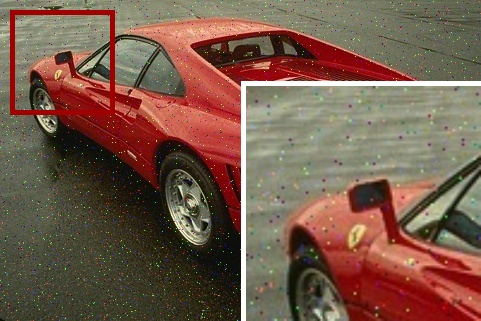
\includegraphics[width=\textwidth]{./figures/sensor/berkeley/29030_noisy_frame.jpg}\vspace{0.1cm}\\
    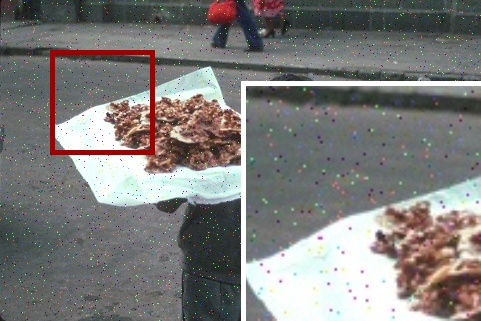
\includegraphics[width=\textwidth]{./figures/sensor/berkeley/90076_noisy_frame.jpg}\vspace{0.1cm}\\
    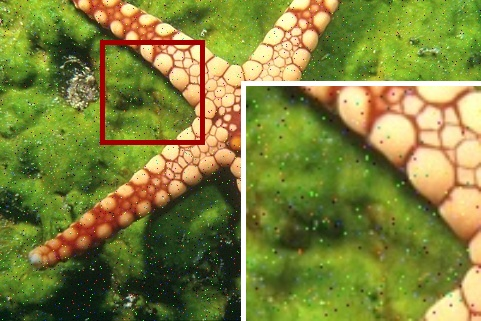
\includegraphics[width=\textwidth]{./figures/sensor/berkeley/12003_noisy_frame.jpg}\vspace{0.1cm}\\
    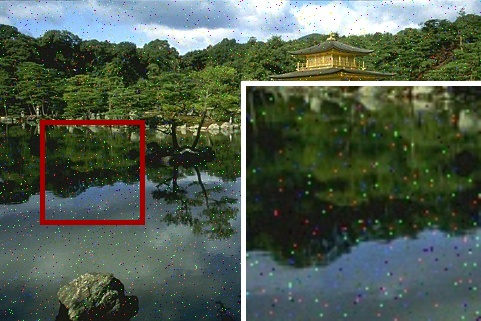
\includegraphics[width=\textwidth]{./figures/sensor/berkeley/65010_noisy_frame.jpg}\vspace{0.1cm}\\
    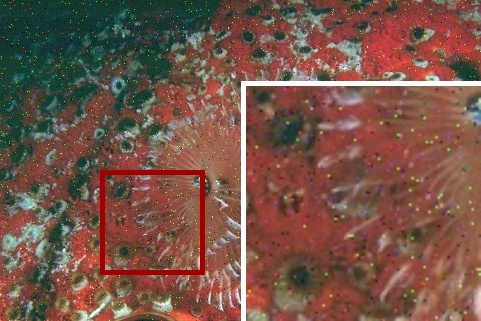
\includegraphics[width=\textwidth]{./figures/sensor/berkeley/12084_noisy_frame.jpg}\vspace{0.1cm}\\
    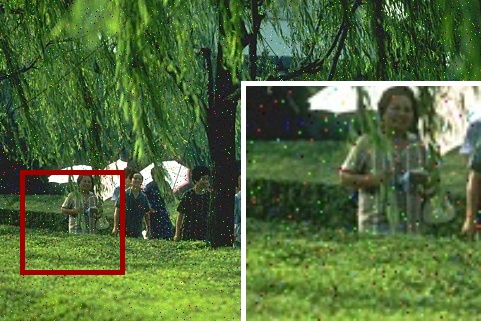
\includegraphics[width=\textwidth]{./figures/sensor/berkeley/65033_noisy_frame.jpg}\vspace{0.1cm}\\
    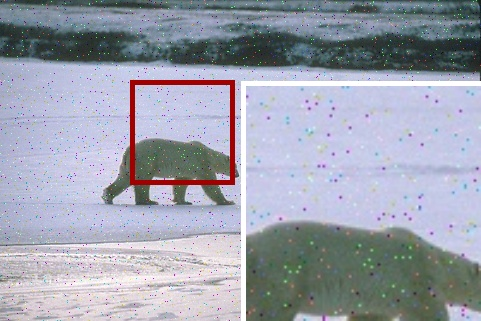
\includegraphics[width=\textwidth]{./figures/sensor/berkeley/100007_noisy_frame.jpg}%
    \caption{Noisy image.}
  \end{subfigure}\hfill
  \begin{subfigure}[]{0.22\textwidth}
    \centering
    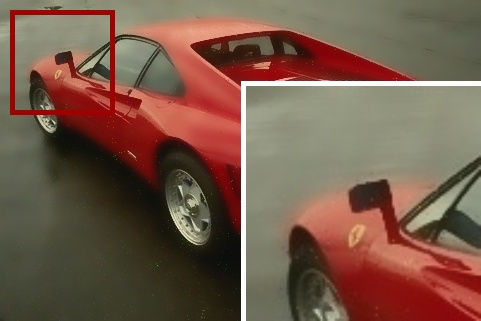
\includegraphics[width=\textwidth]{./figures/sensor/berkeley/29030_bilateral_frame.jpg}\vspace{0.1cm}\\
    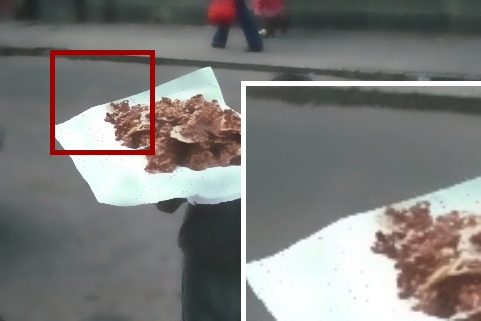
\includegraphics[width=\textwidth]{./figures/sensor/berkeley/90076_bilateral_frame.jpg}\vspace{0.1cm}\\
    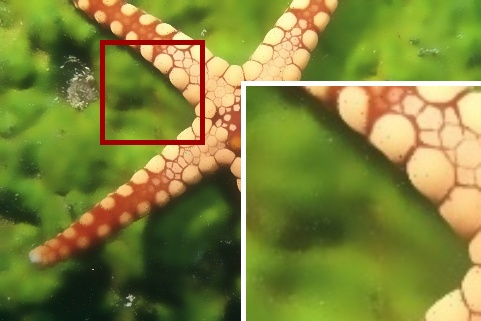
\includegraphics[width=\textwidth]{./figures/sensor/berkeley/12003_bilateral_frame.jpg}\vspace{0.1cm}\\
    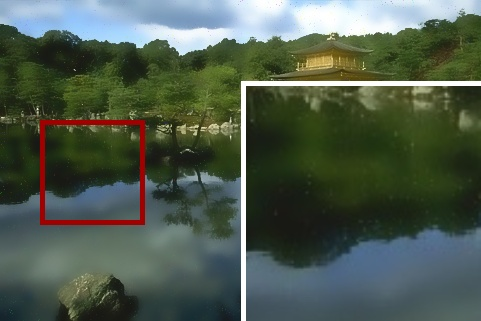
\includegraphics[width=\textwidth]{./figures/sensor/berkeley/65010_bilateral_frame.jpg}\vspace{0.1cm}\\
    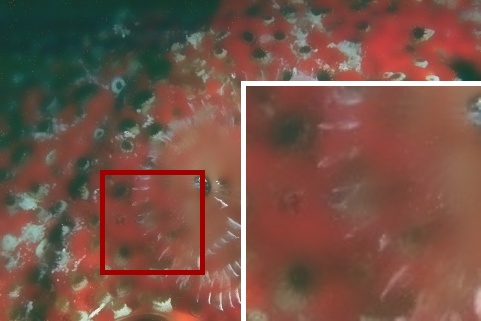
\includegraphics[width=\textwidth]{./figures/sensor/berkeley/12084_bilateral_frame.jpg}\vspace{0.1cm}\\
    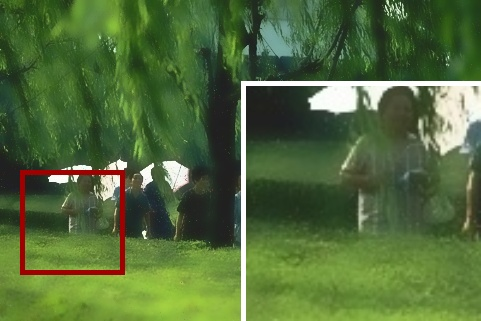
\includegraphics[width=\textwidth]{./figures/sensor/berkeley/65033_bilateral_frame.jpg}\vspace{0.1cm}\\
    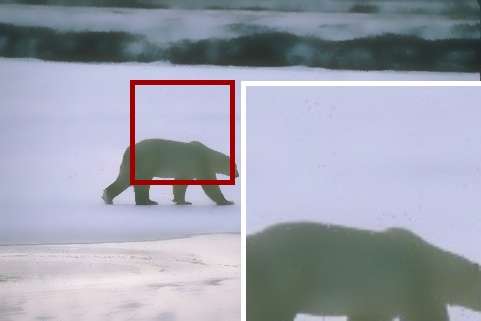
\includegraphics[width=\textwidth]{./figures/sensor/berkeley/100007_bilateral_frame.jpg}%
    \caption{Bilateral Filter.}
  \end{subfigure}\hfill
  \begin{subfigure}[]{0.22\textwidth}
    \centering
    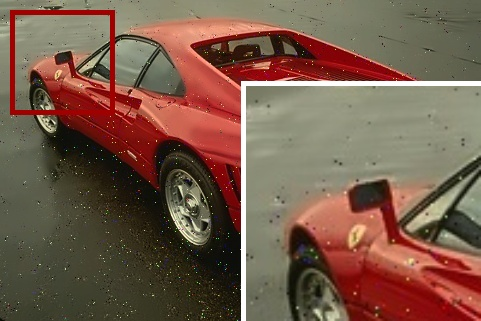
\includegraphics[width=\textwidth]{./figures/sensor/berkeley/29030_nonlocalmeans_frame.jpg}\vspace{0.1cm}\\
    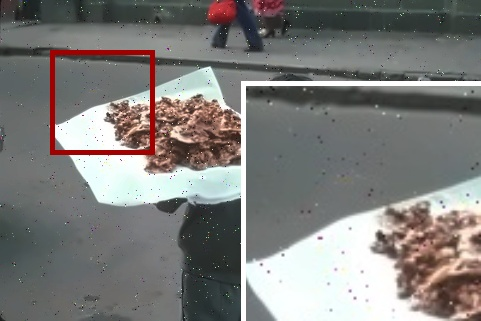
\includegraphics[width=\textwidth]{./figures/sensor/berkeley/90076_nonlocalmeans_frame.jpg}\vspace{0.1cm}\\
    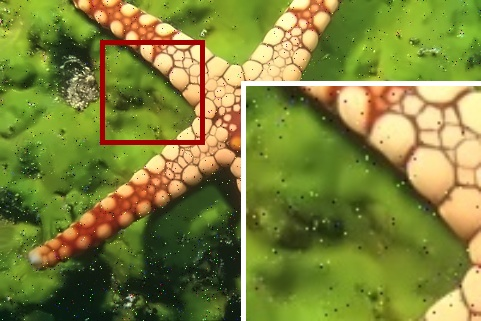
\includegraphics[width=\textwidth]{./figures/sensor/berkeley/12003_nonlocalmeans_frame.jpg}\vspace{0.1cm}\\
    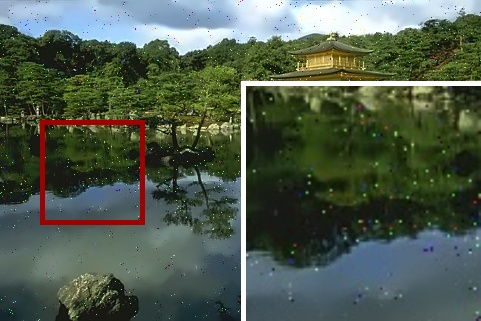
\includegraphics[width=\textwidth]{./figures/sensor/berkeley/65010_nonlocalmeans_frame.jpg}\vspace{0.1cm}\\
    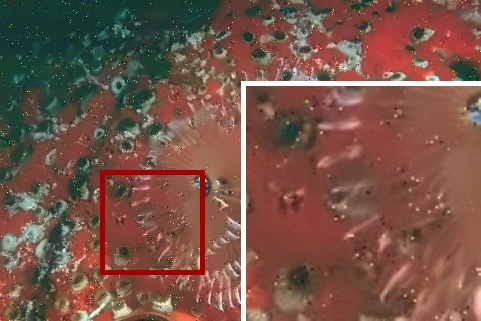
\includegraphics[width=\textwidth]{./figures/sensor/berkeley/12084_nonlocalmeans_frame.jpg}\vspace{0.1cm}\\
    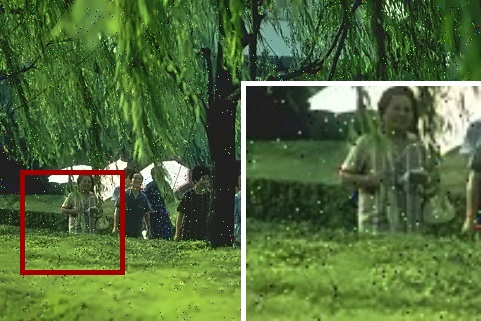
\includegraphics[width=\textwidth]{./figures/sensor/berkeley/65033_nonlocalmeans_frame.jpg}\vspace{0.1cm}\\
    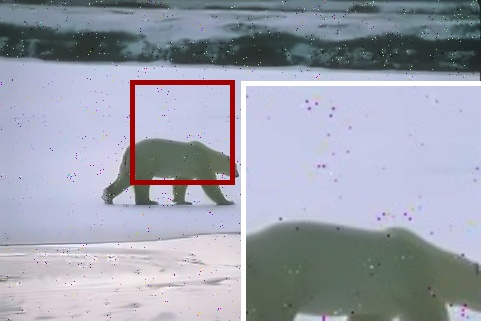
\includegraphics[width=\textwidth]{./figures/sensor/berkeley/100007_nonlocalmeans_frame.jpg}%
    \caption{NLM Filter.}
  \end{subfigure}\hfill
  \begin{subfigure}[]{0.22\textwidth}
    \centering
    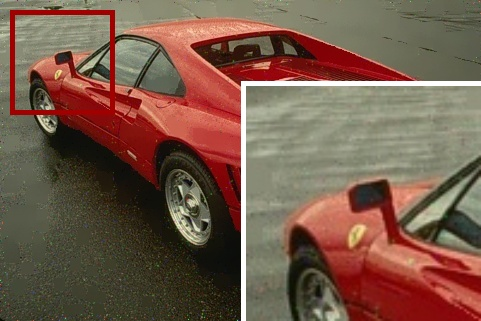
\includegraphics[width=\textwidth]{./figures/sensor/berkeley/29030_edgefilter_frame.jpg}\vspace{0.1cm}\\
    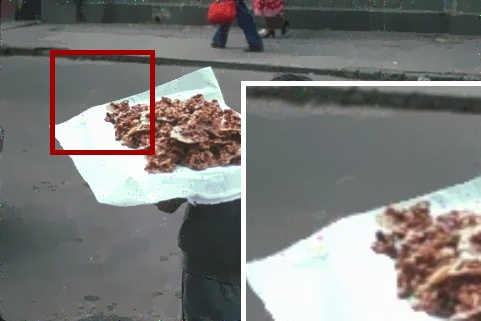
\includegraphics[width=\textwidth]{./figures/sensor/berkeley/90076_edgefilter_frame.jpg}\vspace{0.1cm}\\
    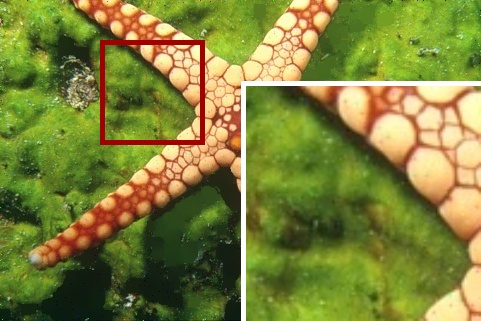
\includegraphics[width=\textwidth]{./figures/sensor/berkeley/12003_edgefilter_frame.jpg}\vspace{0.1cm}\\
    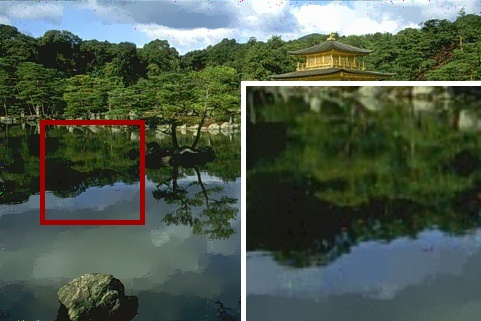
\includegraphics[width=\textwidth]{./figures/sensor/berkeley/65010_edgefilter_frame.jpg}\vspace{0.1cm}\\
    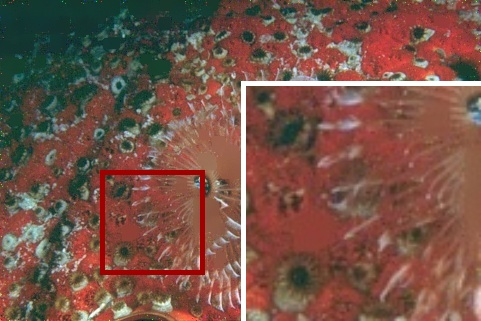
\includegraphics[width=\textwidth]{./figures/sensor/berkeley/12084_edgefilter_frame.jpg}\vspace{0.1cm}\\
    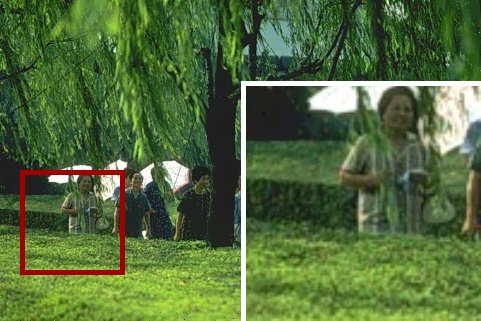
\includegraphics[width=\textwidth]{./figures/sensor/berkeley/65033_edgefilter_frame.jpg}\vspace{0.1cm}\\
    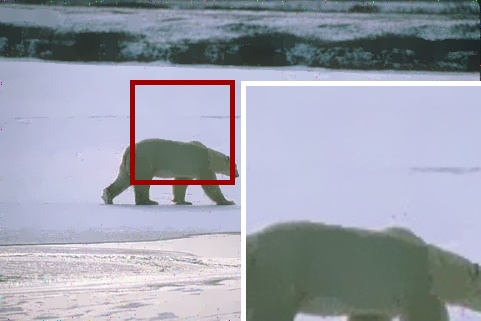
\includegraphics[width=\textwidth]{./figures/sensor/berkeley/100007_edgefilter_frame.jpg}%
    \caption{Proposed EPF.}
  \end{subfigure}%
  \caption{Visual comparison of filter results. Quantitative results are shown in \tabref{tab:experiments_rmsepsnr}. Images taken from Berkeley Image Data Set~\cite{arbelaez2011contour}.}
  \label{fig:sensor_experiments_examples}
\end{figure}

The proposed filter achieves on both data sets the best performance markers. 
In the discussion, see \secref{sec:perception_discussion}, the results are also compared to more recent, state-of-the-art algorithms.

\begin{table}[]
  \centering
  \begin{tabular}{lcccc}
    \toprule
      & \multicolumn{2}{c}{Berkeley Data Set}    & \multicolumn{2}{c}{Coco Data Set}\\
      & RMSE  & PSNR                       & RMSE  & PSNR\\
    \midrule
    Original        & $17.95$ & $23.31$ & $17.31$ & $23.33$\\
    EPF             & \bm{$7.06$} & \bm{$31.05$} & \bm{$7.89$} & \bm{$30.47$}\\
    Bilateral       & $10.41$ & $27.75$ & $10.43$ & $28.01$\\
    Gaussian        & $14.59$ & $25.08$ & $15.69$ & $24.81$\\
    Median          & $14.04$ & $25.63$ & $14.91$ & $25.54$\\
    NLM             & $11.40$ & $26.86$ & $12.28$ & $26.44$\\
    \bottomrule
  \end{tabular}
  \caption{\gls{ac:rmse} and \gls{ac:psnr} computed on the Berkeley Data Set (500 images) and the Coco Data Set (40775 images). The first line ``Original'' refers to the not denoised image. The error is $\pm 0.01$ for all values.}
  \label{tab:experiments_rmsepsnr}
\end{table}





\subsection{Denoising of 1d sensor data}

As already suggested in \figref{fig:sensor_method_example}, \figref{fig:sensor_experiments_subwindowsize}, and \figref{fig:sensor_experiments_threshold}, the filter can also be applied to 1d data. 
This may happen, for example, as a post-processing step for sensor readings. 
The filter is tested on three different settings: first, an alternating line, which switches every 100 samples its height to either $f(x) = f_{min}$ or $f(x) = f_{max}$; second, a sawtooth wave defined by $f(x) = x - \operatorname{floor}_{100}(x)$; and third, a sinusoidal wave $f(x) = \sin{2 \pi x / 250}$ with a wave length of 250 data points.
Every data line consists of a total length of 1000 samples.
To each scenario either Gaussian noise with variance of $\sigma = 10$, salt-and-pepper noise (to 5\% of samples), or both is added. 
Visual examples are shown in \figref{fig:sensor_experiments_1d_altline}, \figref{fig:sensor_experiments_1d_sawtooth}, and \figref{fig:sensor_experiments_1d_sinus}.

Again, the proposed filter ($N = 11$, $\tau = 30$) is compared to a Gaussian blurring filter (kernel: \unit[$7 \times 7$]{px}, $\sigma_{x,y} = 3$), a bilateral filter ($\sigma_c = 30$, $\sigma_s = 30$, and a median filter (kernel size: \unit[$9$]{px}). 
\gls{ac:rmse} and \gls{ac:psnr} is computed according to \eqnref{eq:rmse} and \eqnref{eq:psnr}.
On each setting 1000 trials are performed and averaged.
Results are shown in \tabref{tab:experiments_1d_rmsepsnr}.

In almost all experiments \gls{ac:epf} outperforms other standard 1d filtering methods.
While the median filter performs very well on salt-and-pepper noise, it is not edge preserving and thus introduces artefacts on edges.
The bilateral filter on the other hand, handles edges very well, but has significant trouble with removing salt-and-pepper noise.
The proposed \gls{ac:epf} filter performs well on both, Gaussian and salt-and-pepper noise and is edge preserving.

  \begin{table}[]
  \centering
  \begin{tabular}{c l cc|cc|cc}
    \toprule
    && \multicolumn{2}{c}{Gauss}    & \multicolumn{2}{c}{s\&p}& \multicolumn{2}{c}{Gauss and s\&p}                \\
    &             & RMSE         & PSNR          & RMSE          & PSNR          & RMSE          & PSNR           \\
    \midrule
    \multirow{5}{*}{\rotatebox[origin=c]{90}{\makecell{1) Alternating\\Line \vspace{0.25cm}\\ 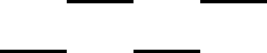
\includegraphics[width=1.5cm]{./figures/sensor/experiments_alternatingline.png}}}} & No denoising & $10.0$       & $22.3$        & $15.2$        & $16.4$         & $18.1$        & $17.2$        \\
    &EPF          & \bm{$2.6$}   & \bm{$32.3}$   & \bm{$3.9$}    & \bm{$28.5$}    & \bm{$5.1$}    & \bm{$26.7$}   \\
    &Bilateral    & $6.9$        & $25.3$        & $15.2$        & $16.4$         & $16.5$        & $17.7$        \\
    &Gaussian     & $6.0$        & $25.3$        &  $7.8$        & $22.2$         &  $8.7$        & $22.1$        \\
    &Median       & $5.1$        & $26.8$        &  $4.1$        & $27.9$         &  $6.0$        & $25.4$        \\
    \midrule
    \multirow{5}{*}{\rotatebox[origin=c]{90}{\makecell{2) Sawtooth\\Wave \vspace{0.25cm}\\ 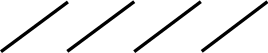
\includegraphics[width=1.5cm]{./figures/sensor/experiments_sawtooth.png}}}} & No denoising &  $10.0$       & $21.6$        & $14.1$        & $17.1$        & $17.1$        & $17.0$        \\
    &EPF          &  \bm{$3.7$}   & \bm{$29.3$}   & \bm{$4.6$}    & \bm{$26.5$}   & \bm{$6.6$}    & \bm{$24.5$}   \\
    &Bilateral    &  $7.0$        & $24.4$        & $14.0$        & $17.1$        & $15.5$        & $17.5$        \\
    &Gaussian     &  $7.6$        & $22.6$        &  $8.8$        & $20.9$        &  $9.6$        & $20.6$        \\
    &Median       &  $5.7$        & $25.2$        &  $5.8$        & $24.9$        &  $7.4$        & $23.1$        \\
    \midrule
    \multirow{5}{*}{\rotatebox[origin=c]{90}{\makecell{3) Sinusoidal\\Wave \vspace{0.25cm}\\ 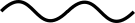
\includegraphics[width=1.5cm]{./figures/sensor/experiments_sinusoidal.png}}}} & No denoising & $10.0$        & $20.1$        & $12.9$        & $17.8$        & $16.1$        & $16.0$        \\
    &EPF          & \bm{$2.7$}    & \bm{$29.5$}   &  $2.6$        & $29.8$        & \bm{$4.4$}    & \bm{$25.6$}   \\
    &Bilateral    & $6.7$         & $23.0$        & $12.8$        & $17.9$        & $14.4$        & $16.9$        \\
    &Gaussian     & $3.9$         & $26.7$        &  $5.0$        & $24.2$        &  $6.3$        & $22.6$        \\
    &Median       & $4.1$         & $26.1$        & \bm{$0.6$}    & \bm{$46.1$}   &  $4.5$        & $25.6$        \\
    \bottomrule
  \end{tabular}
  \caption{Comparison of \gls{ac:rmse} and \gls{ac:psnr} computed on three different scenarios: 1) an alternating line, 2) a sawtooth wave, and 3) a sinusoidal wave. To each scene three different noise types (Gaussian, salt-and-pepper (s\&p), or both) are added, resulting in 9 different experiments. Each experiment is repeated 1000 times and averaged; the error is $\pm 0.1$ for all values.}
  \label{tab:experiments_1d_rmsepsnr}
\end{table}

\begin{figure}[]
  \centering
  \begin{subfigure}[]{\textwidth}
    \centering
    \begin{tikzpicture}[gnuplot]
%% generated with GNUPLOT 5.2p2 (Gentoo revision r0) (Lua 5.1; terminal rev. 99, script rev. 102)
%% Thu 28 Jun 2018 01:37:10 PM CEST
\gpcolor{color=gp lt color axes}
\gpsetlinetype{gp lt axes}
\gpsetdashtype{gp dt axes}
\gpsetlinewidth{0.50}
\draw[gp path] (1.564,1.898)--(13.564,1.898);
\gpcolor{color=gp lt color border}
\gpsetlinetype{gp lt border}
\gpsetdashtype{gp dt solid}
\gpsetlinewidth{1.00}
\draw[gp path] (1.564,1.898)--(1.777,1.898);
\node[gp node right] at (1.346,1.898) {$0$};
\gpcolor{color=gp lt color axes}
\gpsetlinetype{gp lt axes}
\gpsetdashtype{gp dt axes}
\gpsetlinewidth{0.50}
\draw[gp path] (1.564,2.399)--(13.564,2.399);
\gpcolor{color=gp lt color border}
\gpsetlinetype{gp lt border}
\gpsetdashtype{gp dt solid}
\gpsetlinewidth{1.00}
\draw[gp path] (1.564,2.399)--(1.777,2.399);
\node[gp node right] at (1.346,2.399) {$20$};
\gpcolor{color=gp lt color axes}
\gpsetlinetype{gp lt axes}
\gpsetdashtype{gp dt axes}
\gpsetlinewidth{0.50}
\draw[gp path] (1.564,2.898)--(13.564,2.898);
\gpcolor{color=gp lt color border}
\gpsetlinetype{gp lt border}
\gpsetdashtype{gp dt solid}
\gpsetlinewidth{1.00}
\draw[gp path] (1.564,2.898)--(1.777,2.898);
\node[gp node right] at (1.346,2.898) {$40$};
\gpcolor{color=gp lt color axes}
\gpsetlinetype{gp lt axes}
\gpsetdashtype{gp dt axes}
\gpsetlinewidth{0.50}
\draw[gp path] (1.564,3.399)--(13.564,3.399);
\gpcolor{color=gp lt color border}
\gpsetlinetype{gp lt border}
\gpsetdashtype{gp dt solid}
\gpsetlinewidth{1.00}
\draw[gp path] (1.564,3.399)--(1.777,3.399);
\node[gp node right] at (1.346,3.399) {$60$};
\gpcolor{color=gp lt color axes}
\gpsetlinetype{gp lt axes}
\gpsetdashtype{gp dt axes}
\gpsetlinewidth{0.50}
\draw[gp path] (1.564,3.900)--(13.564,3.900);
\gpcolor{color=gp lt color border}
\gpsetlinetype{gp lt border}
\gpsetdashtype{gp dt solid}
\gpsetlinewidth{1.00}
\draw[gp path] (1.564,3.900)--(1.777,3.900);
\node[gp node right] at (1.346,3.900) {$80$};
\gpcolor{color=gp lt color axes}
\gpsetlinetype{gp lt axes}
\gpsetdashtype{gp dt axes}
\gpsetlinewidth{0.50}
\draw[gp path] (1.564,4.399)--(13.564,4.399);
\gpcolor{color=gp lt color border}
\gpsetlinetype{gp lt border}
\gpsetdashtype{gp dt solid}
\gpsetlinewidth{1.00}
\draw[gp path] (1.564,4.399)--(1.777,4.399);
\node[gp node right] at (1.346,4.399) {$100$};
\gpcolor{color=gp lt color axes}
\gpsetlinetype{gp lt axes}
\gpsetdashtype{gp dt axes}
\gpsetlinewidth{0.50}
\draw[gp path] (1.564,4.900)--(13.564,4.900);
\gpcolor{color=gp lt color border}
\gpsetlinetype{gp lt border}
\gpsetdashtype{gp dt solid}
\gpsetlinewidth{1.00}
\draw[gp path] (1.564,4.900)--(1.777,4.900);
\node[gp node right] at (1.346,4.900) {$120$};
\draw[gp path] (1.564,1.649)--(1.564,2.020);
\node[gp node center] at (1.564,1.014) {$0$};
\draw[gp path] (3.964,1.649)--(3.964,2.020);
\node[gp node center] at (3.964,1.014) {$50$};
\draw[gp path] (6.364,1.649)--(6.364,2.020);
\node[gp node center] at (6.364,1.014) {$100$};
\draw[gp path] (8.764,1.649)--(8.764,2.020);
\node[gp node center] at (8.764,1.014) {$150$};
\draw[gp path] (11.165,1.649)--(11.165,2.020);
\node[gp node center] at (11.165,1.014) {$200$};
\draw[gp path] (13.564,1.649)--(13.564,2.020);
\node[gp node center] at (13.564,1.014) {$250$};
\draw[gp path] (1.564,5.149)--(1.564,1.649)--(13.564,1.649)--(13.564,5.149)--cycle;
\node[gp node center,rotate=-270] at (0.109,3.399) {Artificial sensor [a.u.]};
\node[gp node center] at (7.564,0.441) {Time [a.u.]};
\node[gp node right] at (6.042,6.604) {Noisy data};
\gpcolor{rgb color={0.667,0.000,0.000}}
\gpsetlinewidth{3.00}
\gpsetpointsize{4.00}
\gppoint{gp mark 2}{(1.564,2.649)}
\gppoint{gp mark 2}{(1.613,2.649)}
\gppoint{gp mark 2}{(1.660,2.649)}
\gppoint{gp mark 2}{(1.709,2.649)}
\gppoint{gp mark 2}{(1.756,2.649)}
\gppoint{gp mark 2}{(1.805,2.649)}
\gppoint{gp mark 2}{(1.852,2.649)}
\gppoint{gp mark 2}{(1.901,2.649)}
\gppoint{gp mark 2}{(1.948,2.649)}
\gppoint{gp mark 2}{(1.997,2.649)}
\gppoint{gp mark 2}{(2.044,2.649)}
\gppoint{gp mark 2}{(2.093,2.649)}
\gppoint{gp mark 2}{(2.140,4.399)}
\gppoint{gp mark 2}{(2.189,2.649)}
\gppoint{gp mark 2}{(2.236,2.649)}
\gppoint{gp mark 2}{(2.285,2.649)}
\gppoint{gp mark 2}{(2.332,2.649)}
\gppoint{gp mark 2}{(2.381,2.649)}
\gppoint{gp mark 2}{(2.428,2.649)}
\gppoint{gp mark 2}{(2.477,2.649)}
\gppoint{gp mark 2}{(2.524,2.649)}
\gppoint{gp mark 2}{(2.573,2.649)}
\gppoint{gp mark 2}{(2.620,2.649)}
\gppoint{gp mark 2}{(2.669,2.649)}
\gppoint{gp mark 2}{(2.716,2.649)}
\gppoint{gp mark 2}{(2.764,2.649)}
\gppoint{gp mark 2}{(2.812,2.649)}
\gppoint{gp mark 2}{(2.860,2.649)}
\gppoint{gp mark 2}{(2.908,2.649)}
\gppoint{gp mark 2}{(2.956,2.649)}
\gppoint{gp mark 2}{(3.004,2.649)}
\gppoint{gp mark 2}{(3.052,2.649)}
\gppoint{gp mark 2}{(3.100,2.649)}
\gppoint{gp mark 2}{(3.148,2.649)}
\gppoint{gp mark 2}{(3.196,2.649)}
\gppoint{gp mark 2}{(3.244,2.649)}
\gppoint{gp mark 2}{(3.292,1.898)}
\gppoint{gp mark 2}{(3.340,2.649)}
\gppoint{gp mark 2}{(3.388,2.649)}
\gppoint{gp mark 2}{(3.436,2.649)}
\gppoint{gp mark 2}{(3.484,2.649)}
\gppoint{gp mark 2}{(3.532,2.649)}
\gppoint{gp mark 2}{(3.580,2.649)}
\gppoint{gp mark 2}{(3.628,2.649)}
\gppoint{gp mark 2}{(3.676,2.649)}
\gppoint{gp mark 2}{(3.724,2.649)}
\gppoint{gp mark 2}{(3.772,2.649)}
\gppoint{gp mark 2}{(3.820,2.649)}
\gppoint{gp mark 2}{(3.868,2.649)}
\gppoint{gp mark 2}{(3.916,2.649)}
\gppoint{gp mark 2}{(3.964,1.898)}
\gppoint{gp mark 2}{(4.012,2.649)}
\gppoint{gp mark 2}{(4.060,2.649)}
\gppoint{gp mark 2}{(4.108,2.649)}
\gppoint{gp mark 2}{(4.156,2.649)}
\gppoint{gp mark 2}{(4.204,2.649)}
\gppoint{gp mark 2}{(4.252,1.898)}
\gppoint{gp mark 2}{(4.300,2.649)}
\gppoint{gp mark 2}{(4.348,2.649)}
\gppoint{gp mark 2}{(4.396,2.649)}
\gppoint{gp mark 2}{(4.444,2.649)}
\gppoint{gp mark 2}{(4.492,2.649)}
\gppoint{gp mark 2}{(4.540,2.649)}
\gppoint{gp mark 2}{(4.588,1.898)}
\gppoint{gp mark 2}{(4.637,2.649)}
\gppoint{gp mark 2}{(4.684,2.649)}
\gppoint{gp mark 2}{(4.733,2.649)}
\gppoint{gp mark 2}{(4.780,2.649)}
\gppoint{gp mark 2}{(4.829,2.649)}
\gppoint{gp mark 2}{(4.876,1.898)}
\gppoint{gp mark 2}{(4.925,2.649)}
\gppoint{gp mark 2}{(4.972,2.649)}
\gppoint{gp mark 2}{(5.021,2.649)}
\gppoint{gp mark 2}{(5.068,2.649)}
\gppoint{gp mark 2}{(5.117,2.649)}
\gppoint{gp mark 2}{(5.164,2.649)}
\gppoint{gp mark 2}{(5.213,2.649)}
\gppoint{gp mark 2}{(5.260,2.649)}
\gppoint{gp mark 2}{(5.309,2.649)}
\gppoint{gp mark 2}{(5.356,4.399)}
\gppoint{gp mark 2}{(5.405,2.649)}
\gppoint{gp mark 2}{(5.452,2.649)}
\gppoint{gp mark 2}{(5.501,2.649)}
\gppoint{gp mark 2}{(5.548,2.649)}
\gppoint{gp mark 2}{(5.597,2.649)}
\gppoint{gp mark 2}{(5.644,2.649)}
\gppoint{gp mark 2}{(5.693,2.649)}
\gppoint{gp mark 2}{(5.740,2.649)}
\gppoint{gp mark 2}{(5.788,2.649)}
\gppoint{gp mark 2}{(5.836,2.649)}
\gppoint{gp mark 2}{(5.884,2.649)}
\gppoint{gp mark 2}{(5.932,2.649)}
\gppoint{gp mark 2}{(5.980,2.649)}
\gppoint{gp mark 2}{(6.028,2.649)}
\gppoint{gp mark 2}{(6.076,2.649)}
\gppoint{gp mark 2}{(6.124,2.649)}
\gppoint{gp mark 2}{(6.172,2.649)}
\gppoint{gp mark 2}{(6.220,2.649)}
\gppoint{gp mark 2}{(6.268,2.649)}
\gppoint{gp mark 2}{(6.316,2.649)}
\gppoint{gp mark 2}{(6.364,4.399)}
\gppoint{gp mark 2}{(6.412,4.399)}
\gppoint{gp mark 2}{(6.460,4.399)}
\gppoint{gp mark 2}{(6.508,4.399)}
\gppoint{gp mark 2}{(6.556,4.399)}
\gppoint{gp mark 2}{(6.604,4.399)}
\gppoint{gp mark 2}{(6.652,4.399)}
\gppoint{gp mark 2}{(6.700,4.399)}
\gppoint{gp mark 2}{(6.748,4.399)}
\gppoint{gp mark 2}{(6.796,4.399)}
\gppoint{gp mark 2}{(6.844,4.399)}
\gppoint{gp mark 2}{(6.892,4.399)}
\gppoint{gp mark 2}{(6.940,4.399)}
\gppoint{gp mark 2}{(6.988,4.399)}
\gppoint{gp mark 2}{(7.036,4.399)}
\gppoint{gp mark 2}{(7.084,4.399)}
\gppoint{gp mark 2}{(7.132,4.399)}
\gppoint{gp mark 2}{(7.180,4.399)}
\gppoint{gp mark 2}{(7.228,4.399)}
\gppoint{gp mark 2}{(7.276,4.399)}
\gppoint{gp mark 2}{(7.324,4.399)}
\gppoint{gp mark 2}{(7.372,4.399)}
\gppoint{gp mark 2}{(7.420,4.399)}
\gppoint{gp mark 2}{(7.468,4.399)}
\gppoint{gp mark 2}{(7.516,4.399)}
\gppoint{gp mark 2}{(7.565,4.399)}
\gppoint{gp mark 2}{(7.612,4.399)}
\gppoint{gp mark 2}{(7.661,4.399)}
\gppoint{gp mark 2}{(7.708,4.399)}
\gppoint{gp mark 2}{(7.757,4.399)}
\gppoint{gp mark 2}{(7.804,4.399)}
\gppoint{gp mark 2}{(7.853,4.399)}
\gppoint{gp mark 2}{(7.900,4.399)}
\gppoint{gp mark 2}{(7.949,4.399)}
\gppoint{gp mark 2}{(7.996,4.399)}
\gppoint{gp mark 2}{(8.045,4.399)}
\gppoint{gp mark 2}{(8.092,4.399)}
\gppoint{gp mark 2}{(8.141,4.399)}
\gppoint{gp mark 2}{(8.188,4.399)}
\gppoint{gp mark 2}{(8.237,4.399)}
\gppoint{gp mark 2}{(8.284,4.399)}
\gppoint{gp mark 2}{(8.333,4.399)}
\gppoint{gp mark 2}{(8.380,4.399)}
\gppoint{gp mark 2}{(8.429,4.399)}
\gppoint{gp mark 2}{(8.476,4.399)}
\gppoint{gp mark 2}{(8.525,4.399)}
\gppoint{gp mark 2}{(8.572,4.399)}
\gppoint{gp mark 2}{(8.621,4.399)}
\gppoint{gp mark 2}{(8.668,4.399)}
\gppoint{gp mark 2}{(8.717,4.399)}
\gppoint{gp mark 2}{(8.764,4.399)}
\gppoint{gp mark 2}{(8.812,4.399)}
\gppoint{gp mark 2}{(8.860,4.399)}
\gppoint{gp mark 2}{(8.908,4.399)}
\gppoint{gp mark 2}{(8.956,4.399)}
\gppoint{gp mark 2}{(9.004,4.399)}
\gppoint{gp mark 2}{(9.052,4.399)}
\gppoint{gp mark 2}{(9.100,4.399)}
\gppoint{gp mark 2}{(9.148,4.399)}
\gppoint{gp mark 2}{(9.196,4.399)}
\gppoint{gp mark 2}{(9.244,4.399)}
\gppoint{gp mark 2}{(9.292,4.399)}
\gppoint{gp mark 2}{(9.340,4.399)}
\gppoint{gp mark 2}{(9.388,4.399)}
\gppoint{gp mark 2}{(9.436,4.399)}
\gppoint{gp mark 2}{(9.484,4.399)}
\gppoint{gp mark 2}{(9.532,4.399)}
\gppoint{gp mark 2}{(9.580,4.399)}
\gppoint{gp mark 2}{(9.628,4.399)}
\gppoint{gp mark 2}{(9.676,4.399)}
\gppoint{gp mark 2}{(9.724,1.898)}
\gppoint{gp mark 2}{(9.772,4.399)}
\gppoint{gp mark 2}{(9.820,4.399)}
\gppoint{gp mark 2}{(9.868,4.399)}
\gppoint{gp mark 2}{(9.916,4.399)}
\gppoint{gp mark 2}{(9.964,4.399)}
\gppoint{gp mark 2}{(10.012,4.399)}
\gppoint{gp mark 2}{(10.060,4.399)}
\gppoint{gp mark 2}{(10.108,4.399)}
\gppoint{gp mark 2}{(10.156,4.399)}
\gppoint{gp mark 2}{(10.204,4.399)}
\gppoint{gp mark 2}{(10.252,4.399)}
\gppoint{gp mark 2}{(10.300,4.399)}
\gppoint{gp mark 2}{(10.348,4.399)}
\gppoint{gp mark 2}{(10.396,4.399)}
\gppoint{gp mark 2}{(10.444,4.399)}
\gppoint{gp mark 2}{(10.492,4.399)}
\gppoint{gp mark 2}{(10.540,4.399)}
\gppoint{gp mark 2}{(10.589,4.399)}
\gppoint{gp mark 2}{(10.636,4.399)}
\gppoint{gp mark 2}{(10.685,4.399)}
\gppoint{gp mark 2}{(10.732,4.399)}
\gppoint{gp mark 2}{(10.781,4.399)}
\gppoint{gp mark 2}{(10.828,4.399)}
\gppoint{gp mark 2}{(10.877,4.399)}
\gppoint{gp mark 2}{(10.924,4.399)}
\gppoint{gp mark 2}{(10.973,4.399)}
\gppoint{gp mark 2}{(11.020,1.898)}
\gppoint{gp mark 2}{(11.069,4.399)}
\gppoint{gp mark 2}{(11.116,4.399)}
\gppoint{gp mark 2}{(11.165,4.399)}
\gppoint{gp mark 2}{(11.212,2.649)}
\gppoint{gp mark 2}{(11.261,4.399)}
\gppoint{gp mark 2}{(11.308,2.649)}
\gppoint{gp mark 2}{(11.357,2.649)}
\gppoint{gp mark 2}{(11.404,2.649)}
\gppoint{gp mark 2}{(11.453,2.649)}
\gppoint{gp mark 2}{(11.500,2.649)}
\gppoint{gp mark 2}{(11.549,2.649)}
\gppoint{gp mark 2}{(11.596,2.649)}
\gppoint{gp mark 2}{(11.645,2.649)}
\gppoint{gp mark 2}{(11.692,2.649)}
\gppoint{gp mark 2}{(11.740,4.399)}
\gppoint{gp mark 2}{(11.788,2.649)}
\gppoint{gp mark 2}{(11.836,2.649)}
\gppoint{gp mark 2}{(11.884,2.649)}
\gppoint{gp mark 2}{(11.932,2.649)}
\gppoint{gp mark 2}{(11.980,2.649)}
\gppoint{gp mark 2}{(12.028,2.649)}
\gppoint{gp mark 2}{(12.076,2.649)}
\gppoint{gp mark 2}{(12.124,2.649)}
\gppoint{gp mark 2}{(12.172,2.649)}
\gppoint{gp mark 2}{(12.220,2.649)}
\gppoint{gp mark 2}{(12.268,2.649)}
\gppoint{gp mark 2}{(12.316,4.399)}
\gppoint{gp mark 2}{(12.364,2.649)}
\gppoint{gp mark 2}{(12.412,2.649)}
\gppoint{gp mark 2}{(12.460,2.649)}
\gppoint{gp mark 2}{(12.508,2.649)}
\gppoint{gp mark 2}{(12.556,2.649)}
\gppoint{gp mark 2}{(12.604,1.898)}
\gppoint{gp mark 2}{(12.652,2.649)}
\gppoint{gp mark 2}{(12.700,2.649)}
\gppoint{gp mark 2}{(12.748,2.649)}
\gppoint{gp mark 2}{(12.796,2.649)}
\gppoint{gp mark 2}{(12.844,2.649)}
\gppoint{gp mark 2}{(12.892,2.649)}
\gppoint{gp mark 2}{(12.940,2.649)}
\gppoint{gp mark 2}{(12.988,4.399)}
\gppoint{gp mark 2}{(13.036,2.649)}
\gppoint{gp mark 2}{(13.084,2.649)}
\gppoint{gp mark 2}{(13.132,2.649)}
\gppoint{gp mark 2}{(13.180,2.649)}
\gppoint{gp mark 2}{(13.228,2.649)}
\gppoint{gp mark 2}{(13.276,2.649)}
\gppoint{gp mark 2}{(13.324,4.399)}
\gppoint{gp mark 2}{(13.372,2.649)}
\gppoint{gp mark 2}{(13.420,2.649)}
\gppoint{gp mark 2}{(13.468,2.649)}
\gppoint{gp mark 2}{(13.516,2.649)}
\gppoint{gp mark 2}{(13.564,2.649)}
\gppoint{gp mark 2}{(6.803,6.604)}
\gpcolor{color=gp lt color border}
\node[gp node right] at (6.042,6.128) {Bilateral Filter};
\gpcolor{rgb color={0.000,0.000,0.667}}
\gppoint{gp mark 3}{(1.564,2.649)}
\gppoint{gp mark 3}{(1.613,2.649)}
\gppoint{gp mark 3}{(1.660,2.649)}
\gppoint{gp mark 3}{(1.709,2.649)}
\gppoint{gp mark 3}{(1.756,2.649)}
\gppoint{gp mark 3}{(1.805,2.649)}
\gppoint{gp mark 3}{(1.852,2.649)}
\gppoint{gp mark 3}{(1.901,2.649)}
\gppoint{gp mark 3}{(1.948,2.649)}
\gppoint{gp mark 3}{(1.997,2.649)}
\gppoint{gp mark 3}{(2.044,2.649)}
\gppoint{gp mark 3}{(2.093,2.649)}
\gppoint{gp mark 3}{(2.140,4.399)}
\gppoint{gp mark 3}{(2.189,2.649)}
\gppoint{gp mark 3}{(2.236,2.649)}
\gppoint{gp mark 3}{(2.285,2.649)}
\gppoint{gp mark 3}{(2.332,2.649)}
\gppoint{gp mark 3}{(2.381,2.649)}
\gppoint{gp mark 3}{(2.428,2.649)}
\gppoint{gp mark 3}{(2.477,2.649)}
\gppoint{gp mark 3}{(2.524,2.649)}
\gppoint{gp mark 3}{(2.573,2.649)}
\gppoint{gp mark 3}{(2.620,2.649)}
\gppoint{gp mark 3}{(2.669,2.649)}
\gppoint{gp mark 3}{(2.716,2.649)}
\gppoint{gp mark 3}{(2.764,2.649)}
\gppoint{gp mark 3}{(2.812,2.649)}
\gppoint{gp mark 3}{(2.860,2.649)}
\gppoint{gp mark 3}{(2.908,2.649)}
\gppoint{gp mark 3}{(2.956,2.649)}
\gppoint{gp mark 3}{(3.004,2.649)}
\gppoint{gp mark 3}{(3.052,2.649)}
\gppoint{gp mark 3}{(3.100,2.649)}
\gppoint{gp mark 3}{(3.148,2.649)}
\gppoint{gp mark 3}{(3.196,2.649)}
\gppoint{gp mark 3}{(3.244,2.649)}
\gppoint{gp mark 3}{(3.292,1.948)}
\gppoint{gp mark 3}{(3.340,2.649)}
\gppoint{gp mark 3}{(3.388,2.649)}
\gppoint{gp mark 3}{(3.436,2.649)}
\gppoint{gp mark 3}{(3.484,2.649)}
\gppoint{gp mark 3}{(3.532,2.649)}
\gppoint{gp mark 3}{(3.580,2.649)}
\gppoint{gp mark 3}{(3.628,2.649)}
\gppoint{gp mark 3}{(3.676,2.649)}
\gppoint{gp mark 3}{(3.724,2.649)}
\gppoint{gp mark 3}{(3.772,2.649)}
\gppoint{gp mark 3}{(3.820,2.649)}
\gppoint{gp mark 3}{(3.868,2.649)}
\gppoint{gp mark 3}{(3.916,2.649)}
\gppoint{gp mark 3}{(3.964,1.948)}
\gppoint{gp mark 3}{(4.012,2.649)}
\gppoint{gp mark 3}{(4.060,2.647)}
\gppoint{gp mark 3}{(4.108,2.647)}
\gppoint{gp mark 3}{(4.156,2.647)}
\gppoint{gp mark 3}{(4.204,2.649)}
\gppoint{gp mark 3}{(4.252,1.948)}
\gppoint{gp mark 3}{(4.300,2.649)}
\gppoint{gp mark 3}{(4.348,2.649)}
\gppoint{gp mark 3}{(4.396,2.647)}
\gppoint{gp mark 3}{(4.444,2.647)}
\gppoint{gp mark 3}{(4.492,2.649)}
\gppoint{gp mark 3}{(4.540,2.649)}
\gppoint{gp mark 3}{(4.588,1.948)}
\gppoint{gp mark 3}{(4.637,2.649)}
\gppoint{gp mark 3}{(4.684,2.647)}
\gppoint{gp mark 3}{(4.733,2.647)}
\gppoint{gp mark 3}{(4.780,2.647)}
\gppoint{gp mark 3}{(4.829,2.649)}
\gppoint{gp mark 3}{(4.876,1.948)}
\gppoint{gp mark 3}{(4.925,2.649)}
\gppoint{gp mark 3}{(4.972,2.649)}
\gppoint{gp mark 3}{(5.021,2.649)}
\gppoint{gp mark 3}{(5.068,2.649)}
\gppoint{gp mark 3}{(5.117,2.649)}
\gppoint{gp mark 3}{(5.164,2.649)}
\gppoint{gp mark 3}{(5.213,2.649)}
\gppoint{gp mark 3}{(5.260,2.649)}
\gppoint{gp mark 3}{(5.309,2.649)}
\gppoint{gp mark 3}{(5.356,4.399)}
\gppoint{gp mark 3}{(5.405,2.649)}
\gppoint{gp mark 3}{(5.452,2.649)}
\gppoint{gp mark 3}{(5.501,2.649)}
\gppoint{gp mark 3}{(5.548,2.649)}
\gppoint{gp mark 3}{(5.597,2.649)}
\gppoint{gp mark 3}{(5.644,2.649)}
\gppoint{gp mark 3}{(5.693,2.649)}
\gppoint{gp mark 3}{(5.740,2.649)}
\gppoint{gp mark 3}{(5.788,2.649)}
\gppoint{gp mark 3}{(5.836,2.649)}
\gppoint{gp mark 3}{(5.884,2.649)}
\gppoint{gp mark 3}{(5.932,2.649)}
\gppoint{gp mark 3}{(5.980,2.649)}
\gppoint{gp mark 3}{(6.028,2.649)}
\gppoint{gp mark 3}{(6.076,2.649)}
\gppoint{gp mark 3}{(6.124,2.649)}
\gppoint{gp mark 3}{(6.172,2.649)}
\gppoint{gp mark 3}{(6.220,2.649)}
\gppoint{gp mark 3}{(6.268,2.649)}
\gppoint{gp mark 3}{(6.316,2.649)}
\gppoint{gp mark 3}{(6.364,4.399)}
\gppoint{gp mark 3}{(6.412,4.399)}
\gppoint{gp mark 3}{(6.460,4.399)}
\gppoint{gp mark 3}{(6.508,4.399)}
\gppoint{gp mark 3}{(6.556,4.399)}
\gppoint{gp mark 3}{(6.604,4.399)}
\gppoint{gp mark 3}{(6.652,4.399)}
\gppoint{gp mark 3}{(6.700,4.399)}
\gppoint{gp mark 3}{(6.748,4.399)}
\gppoint{gp mark 3}{(6.796,4.399)}
\gppoint{gp mark 3}{(6.844,4.399)}
\gppoint{gp mark 3}{(6.892,4.399)}
\gppoint{gp mark 3}{(6.940,4.399)}
\gppoint{gp mark 3}{(6.988,4.399)}
\gppoint{gp mark 3}{(7.036,4.399)}
\gppoint{gp mark 3}{(7.084,4.399)}
\gppoint{gp mark 3}{(7.132,4.399)}
\gppoint{gp mark 3}{(7.180,4.399)}
\gppoint{gp mark 3}{(7.228,4.399)}
\gppoint{gp mark 3}{(7.276,4.399)}
\gppoint{gp mark 3}{(7.324,4.399)}
\gppoint{gp mark 3}{(7.372,4.399)}
\gppoint{gp mark 3}{(7.420,4.399)}
\gppoint{gp mark 3}{(7.468,4.399)}
\gppoint{gp mark 3}{(7.516,4.399)}
\gppoint{gp mark 3}{(7.565,4.399)}
\gppoint{gp mark 3}{(7.612,4.399)}
\gppoint{gp mark 3}{(7.661,4.399)}
\gppoint{gp mark 3}{(7.708,4.399)}
\gppoint{gp mark 3}{(7.757,4.399)}
\gppoint{gp mark 3}{(7.804,4.399)}
\gppoint{gp mark 3}{(7.853,4.399)}
\gppoint{gp mark 3}{(7.900,4.399)}
\gppoint{gp mark 3}{(7.949,4.399)}
\gppoint{gp mark 3}{(7.996,4.399)}
\gppoint{gp mark 3}{(8.045,4.399)}
\gppoint{gp mark 3}{(8.092,4.399)}
\gppoint{gp mark 3}{(8.141,4.399)}
\gppoint{gp mark 3}{(8.188,4.399)}
\gppoint{gp mark 3}{(8.237,4.399)}
\gppoint{gp mark 3}{(8.284,4.399)}
\gppoint{gp mark 3}{(8.333,4.399)}
\gppoint{gp mark 3}{(8.380,4.399)}
\gppoint{gp mark 3}{(8.429,4.399)}
\gppoint{gp mark 3}{(8.476,4.399)}
\gppoint{gp mark 3}{(8.525,4.399)}
\gppoint{gp mark 3}{(8.572,4.399)}
\gppoint{gp mark 3}{(8.621,4.399)}
\gppoint{gp mark 3}{(8.668,4.399)}
\gppoint{gp mark 3}{(8.717,4.399)}
\gppoint{gp mark 3}{(8.764,4.399)}
\gppoint{gp mark 3}{(8.812,4.399)}
\gppoint{gp mark 3}{(8.860,4.399)}
\gppoint{gp mark 3}{(8.908,4.399)}
\gppoint{gp mark 3}{(8.956,4.399)}
\gppoint{gp mark 3}{(9.004,4.399)}
\gppoint{gp mark 3}{(9.052,4.399)}
\gppoint{gp mark 3}{(9.100,4.399)}
\gppoint{gp mark 3}{(9.148,4.399)}
\gppoint{gp mark 3}{(9.196,4.399)}
\gppoint{gp mark 3}{(9.244,4.399)}
\gppoint{gp mark 3}{(9.292,4.399)}
\gppoint{gp mark 3}{(9.340,4.399)}
\gppoint{gp mark 3}{(9.388,4.399)}
\gppoint{gp mark 3}{(9.436,4.399)}
\gppoint{gp mark 3}{(9.484,4.399)}
\gppoint{gp mark 3}{(9.532,4.399)}
\gppoint{gp mark 3}{(9.580,4.399)}
\gppoint{gp mark 3}{(9.628,4.399)}
\gppoint{gp mark 3}{(9.676,4.399)}
\gppoint{gp mark 3}{(9.724,1.898)}
\gppoint{gp mark 3}{(9.772,4.399)}
\gppoint{gp mark 3}{(9.820,4.399)}
\gppoint{gp mark 3}{(9.868,4.399)}
\gppoint{gp mark 3}{(9.916,4.399)}
\gppoint{gp mark 3}{(9.964,4.399)}
\gppoint{gp mark 3}{(10.012,4.399)}
\gppoint{gp mark 3}{(10.060,4.399)}
\gppoint{gp mark 3}{(10.108,4.399)}
\gppoint{gp mark 3}{(10.156,4.399)}
\gppoint{gp mark 3}{(10.204,4.399)}
\gppoint{gp mark 3}{(10.252,4.399)}
\gppoint{gp mark 3}{(10.300,4.399)}
\gppoint{gp mark 3}{(10.348,4.399)}
\gppoint{gp mark 3}{(10.396,4.399)}
\gppoint{gp mark 3}{(10.444,4.399)}
\gppoint{gp mark 3}{(10.492,4.399)}
\gppoint{gp mark 3}{(10.540,4.399)}
\gppoint{gp mark 3}{(10.589,4.399)}
\gppoint{gp mark 3}{(10.636,4.399)}
\gppoint{gp mark 3}{(10.685,4.399)}
\gppoint{gp mark 3}{(10.732,4.399)}
\gppoint{gp mark 3}{(10.781,4.399)}
\gppoint{gp mark 3}{(10.828,4.399)}
\gppoint{gp mark 3}{(10.877,4.399)}
\gppoint{gp mark 3}{(10.924,4.399)}
\gppoint{gp mark 3}{(10.973,4.399)}
\gppoint{gp mark 3}{(11.020,1.905)}
\gppoint{gp mark 3}{(11.069,4.399)}
\gppoint{gp mark 3}{(11.116,4.399)}
\gppoint{gp mark 3}{(11.165,4.399)}
\gppoint{gp mark 3}{(11.212,2.647)}
\gppoint{gp mark 3}{(11.261,4.399)}
\gppoint{gp mark 3}{(11.308,2.649)}
\gppoint{gp mark 3}{(11.357,2.649)}
\gppoint{gp mark 3}{(11.404,2.649)}
\gppoint{gp mark 3}{(11.453,2.649)}
\gppoint{gp mark 3}{(11.500,2.649)}
\gppoint{gp mark 3}{(11.549,2.649)}
\gppoint{gp mark 3}{(11.596,2.649)}
\gppoint{gp mark 3}{(11.645,2.649)}
\gppoint{gp mark 3}{(11.692,2.649)}
\gppoint{gp mark 3}{(11.740,4.399)}
\gppoint{gp mark 3}{(11.788,2.649)}
\gppoint{gp mark 3}{(11.836,2.649)}
\gppoint{gp mark 3}{(11.884,2.649)}
\gppoint{gp mark 3}{(11.932,2.649)}
\gppoint{gp mark 3}{(11.980,2.649)}
\gppoint{gp mark 3}{(12.028,2.649)}
\gppoint{gp mark 3}{(12.076,2.649)}
\gppoint{gp mark 3}{(12.124,2.649)}
\gppoint{gp mark 3}{(12.172,2.649)}
\gppoint{gp mark 3}{(12.220,2.649)}
\gppoint{gp mark 3}{(12.268,2.649)}
\gppoint{gp mark 3}{(12.316,4.399)}
\gppoint{gp mark 3}{(12.364,2.649)}
\gppoint{gp mark 3}{(12.412,2.649)}
\gppoint{gp mark 3}{(12.460,2.649)}
\gppoint{gp mark 3}{(12.508,2.649)}
\gppoint{gp mark 3}{(12.556,2.649)}
\gppoint{gp mark 3}{(12.604,1.948)}
\gppoint{gp mark 3}{(12.652,2.649)}
\gppoint{gp mark 3}{(12.700,2.649)}
\gppoint{gp mark 3}{(12.748,2.649)}
\gppoint{gp mark 3}{(12.796,2.649)}
\gppoint{gp mark 3}{(12.844,2.649)}
\gppoint{gp mark 3}{(12.892,2.649)}
\gppoint{gp mark 3}{(12.940,2.649)}
\gppoint{gp mark 3}{(12.988,4.399)}
\gppoint{gp mark 3}{(13.036,2.649)}
\gppoint{gp mark 3}{(13.084,2.649)}
\gppoint{gp mark 3}{(13.132,2.649)}
\gppoint{gp mark 3}{(13.180,2.649)}
\gppoint{gp mark 3}{(13.228,2.649)}
\gppoint{gp mark 3}{(13.276,2.649)}
\gppoint{gp mark 3}{(13.324,4.399)}
\gppoint{gp mark 3}{(13.372,2.649)}
\gppoint{gp mark 3}{(13.420,2.649)}
\gppoint{gp mark 3}{(13.468,2.649)}
\gppoint{gp mark 3}{(13.516,2.649)}
\gppoint{gp mark 3}{(13.564,2.649)}
\gppoint{gp mark 3}{(6.803,6.128)}
\gpcolor{color=gp lt color border}
\node[gp node right] at (6.042,5.652) {Gaussian Filter};
\gpcolor{rgb color={0.902,0.624,0.000}}
\gpsetlinewidth{1.00}
\gppoint{gp mark 4}{(1.564,2.649)}
\gppoint{gp mark 4}{(1.613,2.649)}
\gppoint{gp mark 4}{(1.660,2.649)}
\gppoint{gp mark 4}{(1.709,2.649)}
\gppoint{gp mark 4}{(1.756,2.649)}
\gppoint{gp mark 4}{(1.805,2.649)}
\gppoint{gp mark 4}{(1.852,2.649)}
\gppoint{gp mark 4}{(1.901,2.649)}
\gppoint{gp mark 4}{(1.948,2.649)}
\gppoint{gp mark 4}{(1.997,2.834)}
\gppoint{gp mark 4}{(2.044,2.894)}
\gppoint{gp mark 4}{(2.093,2.939)}
\gppoint{gp mark 4}{(2.140,2.956)}
\gppoint{gp mark 4}{(2.189,2.939)}
\gppoint{gp mark 4}{(2.236,2.894)}
\gppoint{gp mark 4}{(2.285,2.834)}
\gppoint{gp mark 4}{(2.332,2.649)}
\gppoint{gp mark 4}{(2.381,2.649)}
\gppoint{gp mark 4}{(2.428,2.649)}
\gppoint{gp mark 4}{(2.477,2.649)}
\gppoint{gp mark 4}{(2.524,2.649)}
\gppoint{gp mark 4}{(2.573,2.649)}
\gppoint{gp mark 4}{(2.620,2.649)}
\gppoint{gp mark 4}{(2.669,2.649)}
\gppoint{gp mark 4}{(2.716,2.649)}
\gppoint{gp mark 4}{(2.764,2.649)}
\gppoint{gp mark 4}{(2.812,2.649)}
\gppoint{gp mark 4}{(2.860,2.649)}
\gppoint{gp mark 4}{(2.908,2.649)}
\gppoint{gp mark 4}{(2.956,2.649)}
\gppoint{gp mark 4}{(3.004,2.649)}
\gppoint{gp mark 4}{(3.052,2.649)}
\gppoint{gp mark 4}{(3.100,2.649)}
\gppoint{gp mark 4}{(3.148,2.568)}
\gppoint{gp mark 4}{(3.196,2.544)}
\gppoint{gp mark 4}{(3.244,2.525)}
\gppoint{gp mark 4}{(3.292,2.517)}
\gppoint{gp mark 4}{(3.340,2.525)}
\gppoint{gp mark 4}{(3.388,2.544)}
\gppoint{gp mark 4}{(3.436,2.568)}
\gppoint{gp mark 4}{(3.484,2.649)}
\gppoint{gp mark 4}{(3.532,2.649)}
\gppoint{gp mark 4}{(3.580,2.649)}
\gppoint{gp mark 4}{(3.628,2.649)}
\gppoint{gp mark 4}{(3.676,2.649)}
\gppoint{gp mark 4}{(3.724,2.649)}
\gppoint{gp mark 4}{(3.772,2.649)}
\gppoint{gp mark 4}{(3.820,2.568)}
\gppoint{gp mark 4}{(3.868,2.544)}
\gppoint{gp mark 4}{(3.916,2.525)}
\gppoint{gp mark 4}{(3.964,2.517)}
\gppoint{gp mark 4}{(4.012,2.525)}
\gppoint{gp mark 4}{(4.060,2.544)}
\gppoint{gp mark 4}{(4.108,2.490)}
\gppoint{gp mark 4}{(4.156,2.544)}
\gppoint{gp mark 4}{(4.204,2.525)}
\gppoint{gp mark 4}{(4.252,2.517)}
\gppoint{gp mark 4}{(4.300,2.525)}
\gppoint{gp mark 4}{(4.348,2.544)}
\gppoint{gp mark 4}{(4.396,2.568)}
\gppoint{gp mark 4}{(4.444,2.568)}
\gppoint{gp mark 4}{(4.492,2.544)}
\gppoint{gp mark 4}{(4.540,2.525)}
\gppoint{gp mark 4}{(4.588,2.517)}
\gppoint{gp mark 4}{(4.637,2.525)}
\gppoint{gp mark 4}{(4.684,2.544)}
\gppoint{gp mark 4}{(4.733,2.490)}
\gppoint{gp mark 4}{(4.780,2.544)}
\gppoint{gp mark 4}{(4.829,2.525)}
\gppoint{gp mark 4}{(4.876,2.517)}
\gppoint{gp mark 4}{(4.925,2.525)}
\gppoint{gp mark 4}{(4.972,2.544)}
\gppoint{gp mark 4}{(5.021,2.568)}
\gppoint{gp mark 4}{(5.068,2.649)}
\gppoint{gp mark 4}{(5.117,2.649)}
\gppoint{gp mark 4}{(5.164,2.649)}
\gppoint{gp mark 4}{(5.213,2.834)}
\gppoint{gp mark 4}{(5.260,2.894)}
\gppoint{gp mark 4}{(5.309,2.939)}
\gppoint{gp mark 4}{(5.356,2.956)}
\gppoint{gp mark 4}{(5.405,2.939)}
\gppoint{gp mark 4}{(5.452,2.894)}
\gppoint{gp mark 4}{(5.501,2.834)}
\gppoint{gp mark 4}{(5.548,2.649)}
\gppoint{gp mark 4}{(5.597,2.649)}
\gppoint{gp mark 4}{(5.644,2.649)}
\gppoint{gp mark 4}{(5.693,2.649)}
\gppoint{gp mark 4}{(5.740,2.649)}
\gppoint{gp mark 4}{(5.788,2.649)}
\gppoint{gp mark 4}{(5.836,2.649)}
\gppoint{gp mark 4}{(5.884,2.649)}
\gppoint{gp mark 4}{(5.932,2.649)}
\gppoint{gp mark 4}{(5.980,2.649)}
\gppoint{gp mark 4}{(6.028,2.649)}
\gppoint{gp mark 4}{(6.076,2.649)}
\gppoint{gp mark 4}{(6.124,2.649)}
\gppoint{gp mark 4}{(6.172,2.649)}
\gppoint{gp mark 4}{(6.220,2.834)}
\gppoint{gp mark 4}{(6.268,3.082)}
\gppoint{gp mark 4}{(6.316,3.370)}
\gppoint{gp mark 4}{(6.364,3.677)}
\gppoint{gp mark 4}{(6.412,3.968)}
\gppoint{gp mark 4}{(6.460,4.213)}
\gppoint{gp mark 4}{(6.508,4.399)}
\gppoint{gp mark 4}{(6.556,4.399)}
\gppoint{gp mark 4}{(6.604,4.399)}
\gppoint{gp mark 4}{(6.652,4.399)}
\gppoint{gp mark 4}{(6.700,4.399)}
\gppoint{gp mark 4}{(6.748,4.399)}
\gppoint{gp mark 4}{(6.796,4.399)}
\gppoint{gp mark 4}{(6.844,4.399)}
\gppoint{gp mark 4}{(6.892,4.399)}
\gppoint{gp mark 4}{(6.940,4.399)}
\gppoint{gp mark 4}{(6.988,4.399)}
\gppoint{gp mark 4}{(7.036,4.399)}
\gppoint{gp mark 4}{(7.084,4.399)}
\gppoint{gp mark 4}{(7.132,4.399)}
\gppoint{gp mark 4}{(7.180,4.399)}
\gppoint{gp mark 4}{(7.228,4.399)}
\gppoint{gp mark 4}{(7.276,4.399)}
\gppoint{gp mark 4}{(7.324,4.399)}
\gppoint{gp mark 4}{(7.372,4.399)}
\gppoint{gp mark 4}{(7.420,4.399)}
\gppoint{gp mark 4}{(7.468,4.399)}
\gppoint{gp mark 4}{(7.516,4.399)}
\gppoint{gp mark 4}{(7.565,4.399)}
\gppoint{gp mark 4}{(7.612,4.399)}
\gppoint{gp mark 4}{(7.661,4.399)}
\gppoint{gp mark 4}{(7.708,4.399)}
\gppoint{gp mark 4}{(7.757,4.399)}
\gppoint{gp mark 4}{(7.804,4.399)}
\gppoint{gp mark 4}{(7.853,4.399)}
\gppoint{gp mark 4}{(7.900,4.399)}
\gppoint{gp mark 4}{(7.949,4.399)}
\gppoint{gp mark 4}{(7.996,4.399)}
\gppoint{gp mark 4}{(8.045,4.399)}
\gppoint{gp mark 4}{(8.092,4.399)}
\gppoint{gp mark 4}{(8.141,4.399)}
\gppoint{gp mark 4}{(8.188,4.399)}
\gppoint{gp mark 4}{(8.237,4.399)}
\gppoint{gp mark 4}{(8.284,4.399)}
\gppoint{gp mark 4}{(8.333,4.399)}
\gppoint{gp mark 4}{(8.380,4.399)}
\gppoint{gp mark 4}{(8.429,4.399)}
\gppoint{gp mark 4}{(8.476,4.399)}
\gppoint{gp mark 4}{(8.525,4.399)}
\gppoint{gp mark 4}{(8.572,4.399)}
\gppoint{gp mark 4}{(8.621,4.399)}
\gppoint{gp mark 4}{(8.668,4.399)}
\gppoint{gp mark 4}{(8.717,4.399)}
\gppoint{gp mark 4}{(8.764,4.399)}
\gppoint{gp mark 4}{(8.812,4.399)}
\gppoint{gp mark 4}{(8.860,4.399)}
\gppoint{gp mark 4}{(8.908,4.399)}
\gppoint{gp mark 4}{(8.956,4.399)}
\gppoint{gp mark 4}{(9.004,4.399)}
\gppoint{gp mark 4}{(9.052,4.399)}
\gppoint{gp mark 4}{(9.100,4.399)}
\gppoint{gp mark 4}{(9.148,4.399)}
\gppoint{gp mark 4}{(9.196,4.399)}
\gppoint{gp mark 4}{(9.244,4.399)}
\gppoint{gp mark 4}{(9.292,4.399)}
\gppoint{gp mark 4}{(9.340,4.399)}
\gppoint{gp mark 4}{(9.388,4.399)}
\gppoint{gp mark 4}{(9.436,4.399)}
\gppoint{gp mark 4}{(9.484,4.399)}
\gppoint{gp mark 4}{(9.532,4.399)}
\gppoint{gp mark 4}{(9.580,4.133)}
\gppoint{gp mark 4}{(9.628,4.048)}
\gppoint{gp mark 4}{(9.676,3.984)}
\gppoint{gp mark 4}{(9.724,3.962)}
\gppoint{gp mark 4}{(9.772,3.984)}
\gppoint{gp mark 4}{(9.820,4.048)}
\gppoint{gp mark 4}{(9.868,4.133)}
\gppoint{gp mark 4}{(9.916,4.399)}
\gppoint{gp mark 4}{(9.964,4.399)}
\gppoint{gp mark 4}{(10.012,4.399)}
\gppoint{gp mark 4}{(10.060,4.399)}
\gppoint{gp mark 4}{(10.108,4.399)}
\gppoint{gp mark 4}{(10.156,4.399)}
\gppoint{gp mark 4}{(10.204,4.399)}
\gppoint{gp mark 4}{(10.252,4.399)}
\gppoint{gp mark 4}{(10.300,4.399)}
\gppoint{gp mark 4}{(10.348,4.399)}
\gppoint{gp mark 4}{(10.396,4.399)}
\gppoint{gp mark 4}{(10.444,4.399)}
\gppoint{gp mark 4}{(10.492,4.399)}
\gppoint{gp mark 4}{(10.540,4.399)}
\gppoint{gp mark 4}{(10.589,4.399)}
\gppoint{gp mark 4}{(10.636,4.399)}
\gppoint{gp mark 4}{(10.685,4.399)}
\gppoint{gp mark 4}{(10.732,4.399)}
\gppoint{gp mark 4}{(10.781,4.399)}
\gppoint{gp mark 4}{(10.828,4.399)}
\gppoint{gp mark 4}{(10.877,4.133)}
\gppoint{gp mark 4}{(10.924,4.048)}
\gppoint{gp mark 4}{(10.973,3.984)}
\gppoint{gp mark 4}{(11.020,3.962)}
\gppoint{gp mark 4}{(11.069,3.799)}
\gppoint{gp mark 4}{(11.116,3.803)}
\gppoint{gp mark 4}{(11.165,3.657)}
\gppoint{gp mark 4}{(11.212,3.661)}
\gppoint{gp mark 4}{(11.261,3.387)}
\gppoint{gp mark 4}{(11.308,3.125)}
\gppoint{gp mark 4}{(11.357,2.894)}
\gppoint{gp mark 4}{(11.404,2.834)}
\gppoint{gp mark 4}{(11.453,2.649)}
\gppoint{gp mark 4}{(11.500,2.649)}
\gppoint{gp mark 4}{(11.549,2.649)}
\gppoint{gp mark 4}{(11.596,2.834)}
\gppoint{gp mark 4}{(11.645,2.894)}
\gppoint{gp mark 4}{(11.692,2.939)}
\gppoint{gp mark 4}{(11.740,2.956)}
\gppoint{gp mark 4}{(11.788,2.939)}
\gppoint{gp mark 4}{(11.836,2.894)}
\gppoint{gp mark 4}{(11.884,2.834)}
\gppoint{gp mark 4}{(11.932,2.649)}
\gppoint{gp mark 4}{(11.980,2.649)}
\gppoint{gp mark 4}{(12.028,2.649)}
\gppoint{gp mark 4}{(12.076,2.649)}
\gppoint{gp mark 4}{(12.124,2.649)}
\gppoint{gp mark 4}{(12.172,2.834)}
\gppoint{gp mark 4}{(12.220,2.894)}
\gppoint{gp mark 4}{(12.268,2.939)}
\gppoint{gp mark 4}{(12.316,2.956)}
\gppoint{gp mark 4}{(12.364,2.939)}
\gppoint{gp mark 4}{(12.412,2.894)}
\gppoint{gp mark 4}{(12.460,2.756)}
\gppoint{gp mark 4}{(12.508,2.544)}
\gppoint{gp mark 4}{(12.556,2.525)}
\gppoint{gp mark 4}{(12.604,2.517)}
\gppoint{gp mark 4}{(12.652,2.525)}
\gppoint{gp mark 4}{(12.700,2.544)}
\gppoint{gp mark 4}{(12.748,2.568)}
\gppoint{gp mark 4}{(12.796,2.649)}
\gppoint{gp mark 4}{(12.844,2.834)}
\gppoint{gp mark 4}{(12.892,2.894)}
\gppoint{gp mark 4}{(12.940,2.939)}
\gppoint{gp mark 4}{(12.988,2.956)}
\gppoint{gp mark 4}{(13.036,2.939)}
\gppoint{gp mark 4}{(13.084,2.894)}
\gppoint{gp mark 4}{(13.132,2.834)}
\gppoint{gp mark 4}{(13.180,2.834)}
\gppoint{gp mark 4}{(13.228,2.894)}
\gppoint{gp mark 4}{(13.276,2.939)}
\gppoint{gp mark 4}{(13.324,2.956)}
\gppoint{gp mark 4}{(13.372,2.939)}
\gppoint{gp mark 4}{(13.420,2.894)}
\gppoint{gp mark 4}{(13.468,2.834)}
\gppoint{gp mark 4}{(13.516,2.649)}
\gppoint{gp mark 4}{(13.564,2.649)}
\gppoint{gp mark 4}{(6.803,5.652)}
\gpcolor{color=gp lt color border}
\node[gp node right] at (10.834,6.604) {Median Filter};
\gpcolor{rgb color={0.941,0.894,0.259}}
\gppoint{gp mark 5}{(1.564,2.649)}
\gppoint{gp mark 5}{(1.613,2.649)}
\gppoint{gp mark 5}{(1.660,2.649)}
\gppoint{gp mark 5}{(1.709,2.649)}
\gppoint{gp mark 5}{(1.756,2.649)}
\gppoint{gp mark 5}{(1.805,2.649)}
\gppoint{gp mark 5}{(1.852,2.649)}
\gppoint{gp mark 5}{(1.901,2.649)}
\gppoint{gp mark 5}{(1.948,2.649)}
\gppoint{gp mark 5}{(1.997,2.649)}
\gppoint{gp mark 5}{(2.044,2.649)}
\gppoint{gp mark 5}{(2.093,2.649)}
\gppoint{gp mark 5}{(2.140,2.649)}
\gppoint{gp mark 5}{(2.189,2.649)}
\gppoint{gp mark 5}{(2.236,2.649)}
\gppoint{gp mark 5}{(2.285,2.649)}
\gppoint{gp mark 5}{(2.332,2.649)}
\gppoint{gp mark 5}{(2.381,2.649)}
\gppoint{gp mark 5}{(2.428,2.649)}
\gppoint{gp mark 5}{(2.477,2.649)}
\gppoint{gp mark 5}{(2.524,2.649)}
\gppoint{gp mark 5}{(2.573,2.649)}
\gppoint{gp mark 5}{(2.620,2.649)}
\gppoint{gp mark 5}{(2.669,2.649)}
\gppoint{gp mark 5}{(2.716,2.649)}
\gppoint{gp mark 5}{(2.764,2.649)}
\gppoint{gp mark 5}{(2.812,2.649)}
\gppoint{gp mark 5}{(2.860,2.649)}
\gppoint{gp mark 5}{(2.908,2.649)}
\gppoint{gp mark 5}{(2.956,2.649)}
\gppoint{gp mark 5}{(3.004,2.649)}
\gppoint{gp mark 5}{(3.052,2.649)}
\gppoint{gp mark 5}{(3.100,2.649)}
\gppoint{gp mark 5}{(3.148,2.649)}
\gppoint{gp mark 5}{(3.196,2.649)}
\gppoint{gp mark 5}{(3.244,2.649)}
\gppoint{gp mark 5}{(3.292,2.649)}
\gppoint{gp mark 5}{(3.340,2.649)}
\gppoint{gp mark 5}{(3.388,2.649)}
\gppoint{gp mark 5}{(3.436,2.649)}
\gppoint{gp mark 5}{(3.484,2.649)}
\gppoint{gp mark 5}{(3.532,2.649)}
\gppoint{gp mark 5}{(3.580,2.649)}
\gppoint{gp mark 5}{(3.628,2.649)}
\gppoint{gp mark 5}{(3.676,2.649)}
\gppoint{gp mark 5}{(3.724,2.649)}
\gppoint{gp mark 5}{(3.772,2.649)}
\gppoint{gp mark 5}{(3.820,2.649)}
\gppoint{gp mark 5}{(3.868,2.649)}
\gppoint{gp mark 5}{(3.916,2.649)}
\gppoint{gp mark 5}{(3.964,2.649)}
\gppoint{gp mark 5}{(4.012,2.649)}
\gppoint{gp mark 5}{(4.060,2.649)}
\gppoint{gp mark 5}{(4.108,2.649)}
\gppoint{gp mark 5}{(4.156,2.649)}
\gppoint{gp mark 5}{(4.204,2.649)}
\gppoint{gp mark 5}{(4.252,2.649)}
\gppoint{gp mark 5}{(4.300,2.649)}
\gppoint{gp mark 5}{(4.348,2.649)}
\gppoint{gp mark 5}{(4.396,2.649)}
\gppoint{gp mark 5}{(4.444,2.649)}
\gppoint{gp mark 5}{(4.492,2.649)}
\gppoint{gp mark 5}{(4.540,2.649)}
\gppoint{gp mark 5}{(4.588,2.649)}
\gppoint{gp mark 5}{(4.637,2.649)}
\gppoint{gp mark 5}{(4.684,2.649)}
\gppoint{gp mark 5}{(4.733,2.649)}
\gppoint{gp mark 5}{(4.780,2.649)}
\gppoint{gp mark 5}{(4.829,2.649)}
\gppoint{gp mark 5}{(4.876,2.649)}
\gppoint{gp mark 5}{(4.925,2.649)}
\gppoint{gp mark 5}{(4.972,2.649)}
\gppoint{gp mark 5}{(5.021,2.649)}
\gppoint{gp mark 5}{(5.068,2.649)}
\gppoint{gp mark 5}{(5.117,2.649)}
\gppoint{gp mark 5}{(5.164,2.649)}
\gppoint{gp mark 5}{(5.213,2.649)}
\gppoint{gp mark 5}{(5.260,2.649)}
\gppoint{gp mark 5}{(5.309,2.649)}
\gppoint{gp mark 5}{(5.356,2.649)}
\gppoint{gp mark 5}{(5.405,2.649)}
\gppoint{gp mark 5}{(5.452,2.649)}
\gppoint{gp mark 5}{(5.501,2.649)}
\gppoint{gp mark 5}{(5.548,2.649)}
\gppoint{gp mark 5}{(5.597,2.649)}
\gppoint{gp mark 5}{(5.644,2.649)}
\gppoint{gp mark 5}{(5.693,2.649)}
\gppoint{gp mark 5}{(5.740,2.649)}
\gppoint{gp mark 5}{(5.788,2.649)}
\gppoint{gp mark 5}{(5.836,2.649)}
\gppoint{gp mark 5}{(5.884,2.649)}
\gppoint{gp mark 5}{(5.932,2.649)}
\gppoint{gp mark 5}{(5.980,2.649)}
\gppoint{gp mark 5}{(6.028,2.649)}
\gppoint{gp mark 5}{(6.076,2.649)}
\gppoint{gp mark 5}{(6.124,2.649)}
\gppoint{gp mark 5}{(6.172,2.649)}
\gppoint{gp mark 5}{(6.220,2.649)}
\gppoint{gp mark 5}{(6.268,2.649)}
\gppoint{gp mark 5}{(6.316,2.649)}
\gppoint{gp mark 5}{(6.364,4.399)}
\gppoint{gp mark 5}{(6.412,4.399)}
\gppoint{gp mark 5}{(6.460,4.399)}
\gppoint{gp mark 5}{(6.508,4.399)}
\gppoint{gp mark 5}{(6.556,4.399)}
\gppoint{gp mark 5}{(6.604,4.399)}
\gppoint{gp mark 5}{(6.652,4.399)}
\gppoint{gp mark 5}{(6.700,4.399)}
\gppoint{gp mark 5}{(6.748,4.399)}
\gppoint{gp mark 5}{(6.796,4.399)}
\gppoint{gp mark 5}{(6.844,4.399)}
\gppoint{gp mark 5}{(6.892,4.399)}
\gppoint{gp mark 5}{(6.940,4.399)}
\gppoint{gp mark 5}{(6.988,4.399)}
\gppoint{gp mark 5}{(7.036,4.399)}
\gppoint{gp mark 5}{(7.084,4.399)}
\gppoint{gp mark 5}{(7.132,4.399)}
\gppoint{gp mark 5}{(7.180,4.399)}
\gppoint{gp mark 5}{(7.228,4.399)}
\gppoint{gp mark 5}{(7.276,4.399)}
\gppoint{gp mark 5}{(7.324,4.399)}
\gppoint{gp mark 5}{(7.372,4.399)}
\gppoint{gp mark 5}{(7.420,4.399)}
\gppoint{gp mark 5}{(7.468,4.399)}
\gppoint{gp mark 5}{(7.516,4.399)}
\gppoint{gp mark 5}{(7.565,4.399)}
\gppoint{gp mark 5}{(7.612,4.399)}
\gppoint{gp mark 5}{(7.661,4.399)}
\gppoint{gp mark 5}{(7.708,4.399)}
\gppoint{gp mark 5}{(7.757,4.399)}
\gppoint{gp mark 5}{(7.804,4.399)}
\gppoint{gp mark 5}{(7.853,4.399)}
\gppoint{gp mark 5}{(7.900,4.399)}
\gppoint{gp mark 5}{(7.949,4.399)}
\gppoint{gp mark 5}{(7.996,4.399)}
\gppoint{gp mark 5}{(8.045,4.399)}
\gppoint{gp mark 5}{(8.092,4.399)}
\gppoint{gp mark 5}{(8.141,4.399)}
\gppoint{gp mark 5}{(8.188,4.399)}
\gppoint{gp mark 5}{(8.237,4.399)}
\gppoint{gp mark 5}{(8.284,4.399)}
\gppoint{gp mark 5}{(8.333,4.399)}
\gppoint{gp mark 5}{(8.380,4.399)}
\gppoint{gp mark 5}{(8.429,4.399)}
\gppoint{gp mark 5}{(8.476,4.399)}
\gppoint{gp mark 5}{(8.525,4.399)}
\gppoint{gp mark 5}{(8.572,4.399)}
\gppoint{gp mark 5}{(8.621,4.399)}
\gppoint{gp mark 5}{(8.668,4.399)}
\gppoint{gp mark 5}{(8.717,4.399)}
\gppoint{gp mark 5}{(8.764,4.399)}
\gppoint{gp mark 5}{(8.812,4.399)}
\gppoint{gp mark 5}{(8.860,4.399)}
\gppoint{gp mark 5}{(8.908,4.399)}
\gppoint{gp mark 5}{(8.956,4.399)}
\gppoint{gp mark 5}{(9.004,4.399)}
\gppoint{gp mark 5}{(9.052,4.399)}
\gppoint{gp mark 5}{(9.100,4.399)}
\gppoint{gp mark 5}{(9.148,4.399)}
\gppoint{gp mark 5}{(9.196,4.399)}
\gppoint{gp mark 5}{(9.244,4.399)}
\gppoint{gp mark 5}{(9.292,4.399)}
\gppoint{gp mark 5}{(9.340,4.399)}
\gppoint{gp mark 5}{(9.388,4.399)}
\gppoint{gp mark 5}{(9.436,4.399)}
\gppoint{gp mark 5}{(9.484,4.399)}
\gppoint{gp mark 5}{(9.532,4.399)}
\gppoint{gp mark 5}{(9.580,4.399)}
\gppoint{gp mark 5}{(9.628,4.399)}
\gppoint{gp mark 5}{(9.676,4.399)}
\gppoint{gp mark 5}{(9.724,4.399)}
\gppoint{gp mark 5}{(9.772,4.399)}
\gppoint{gp mark 5}{(9.820,4.399)}
\gppoint{gp mark 5}{(9.868,4.399)}
\gppoint{gp mark 5}{(9.916,4.399)}
\gppoint{gp mark 5}{(9.964,4.399)}
\gppoint{gp mark 5}{(10.012,4.399)}
\gppoint{gp mark 5}{(10.060,4.399)}
\gppoint{gp mark 5}{(10.108,4.399)}
\gppoint{gp mark 5}{(10.156,4.399)}
\gppoint{gp mark 5}{(10.204,4.399)}
\gppoint{gp mark 5}{(10.252,4.399)}
\gppoint{gp mark 5}{(10.300,4.399)}
\gppoint{gp mark 5}{(10.348,4.399)}
\gppoint{gp mark 5}{(10.396,4.399)}
\gppoint{gp mark 5}{(10.444,4.399)}
\gppoint{gp mark 5}{(10.492,4.399)}
\gppoint{gp mark 5}{(10.540,4.399)}
\gppoint{gp mark 5}{(10.589,4.399)}
\gppoint{gp mark 5}{(10.636,4.399)}
\gppoint{gp mark 5}{(10.685,4.399)}
\gppoint{gp mark 5}{(10.732,4.399)}
\gppoint{gp mark 5}{(10.781,4.399)}
\gppoint{gp mark 5}{(10.828,4.399)}
\gppoint{gp mark 5}{(10.877,4.399)}
\gppoint{gp mark 5}{(10.924,4.399)}
\gppoint{gp mark 5}{(10.973,4.399)}
\gppoint{gp mark 5}{(11.020,4.399)}
\gppoint{gp mark 5}{(11.069,4.399)}
\gppoint{gp mark 5}{(11.116,4.399)}
\gppoint{gp mark 5}{(11.165,4.399)}
\gppoint{gp mark 5}{(11.212,2.649)}
\gppoint{gp mark 5}{(11.261,2.649)}
\gppoint{gp mark 5}{(11.308,2.649)}
\gppoint{gp mark 5}{(11.357,2.649)}
\gppoint{gp mark 5}{(11.404,2.649)}
\gppoint{gp mark 5}{(11.453,2.649)}
\gppoint{gp mark 5}{(11.500,2.649)}
\gppoint{gp mark 5}{(11.549,2.649)}
\gppoint{gp mark 5}{(11.596,2.649)}
\gppoint{gp mark 5}{(11.645,2.649)}
\gppoint{gp mark 5}{(11.692,2.649)}
\gppoint{gp mark 5}{(11.740,2.649)}
\gppoint{gp mark 5}{(11.788,2.649)}
\gppoint{gp mark 5}{(11.836,2.649)}
\gppoint{gp mark 5}{(11.884,2.649)}
\gppoint{gp mark 5}{(11.932,2.649)}
\gppoint{gp mark 5}{(11.980,2.649)}
\gppoint{gp mark 5}{(12.028,2.649)}
\gppoint{gp mark 5}{(12.076,2.649)}
\gppoint{gp mark 5}{(12.124,2.649)}
\gppoint{gp mark 5}{(12.172,2.649)}
\gppoint{gp mark 5}{(12.220,2.649)}
\gppoint{gp mark 5}{(12.268,2.649)}
\gppoint{gp mark 5}{(12.316,2.649)}
\gppoint{gp mark 5}{(12.364,2.649)}
\gppoint{gp mark 5}{(12.412,2.649)}
\gppoint{gp mark 5}{(12.460,2.649)}
\gppoint{gp mark 5}{(12.508,2.649)}
\gppoint{gp mark 5}{(12.556,2.649)}
\gppoint{gp mark 5}{(12.604,2.649)}
\gppoint{gp mark 5}{(12.652,2.649)}
\gppoint{gp mark 5}{(12.700,2.649)}
\gppoint{gp mark 5}{(12.748,2.649)}
\gppoint{gp mark 5}{(12.796,2.649)}
\gppoint{gp mark 5}{(12.844,2.649)}
\gppoint{gp mark 5}{(12.892,2.649)}
\gppoint{gp mark 5}{(12.940,2.649)}
\gppoint{gp mark 5}{(12.988,2.649)}
\gppoint{gp mark 5}{(13.036,2.649)}
\gppoint{gp mark 5}{(13.084,2.649)}
\gppoint{gp mark 5}{(13.132,2.649)}
\gppoint{gp mark 5}{(13.180,2.649)}
\gppoint{gp mark 5}{(13.228,2.649)}
\gppoint{gp mark 5}{(13.276,2.649)}
\gppoint{gp mark 5}{(13.324,2.649)}
\gppoint{gp mark 5}{(13.372,2.649)}
\gppoint{gp mark 5}{(13.420,2.649)}
\gppoint{gp mark 5}{(13.468,2.649)}
\gppoint{gp mark 5}{(13.516,2.649)}
\gppoint{gp mark 5}{(13.564,2.649)}
\gppoint{gp mark 5}{(11.595,6.604)}
\gpcolor{color=gp lt color border}
\node[gp node right] at (10.834,6.128) {EPF};
\gpcolor{rgb color={0.000,0.667,0.000}}
\gpsetlinewidth{3.00}
\gppoint{gp mark 12}{(1.564,2.649)}
\gppoint{gp mark 12}{(1.613,2.649)}
\gppoint{gp mark 12}{(1.660,2.649)}
\gppoint{gp mark 12}{(1.709,2.649)}
\gppoint{gp mark 12}{(1.756,2.649)}
\gppoint{gp mark 12}{(1.805,2.649)}
\gppoint{gp mark 12}{(1.852,2.649)}
\gppoint{gp mark 12}{(1.901,2.649)}
\gppoint{gp mark 12}{(1.948,2.649)}
\gppoint{gp mark 12}{(1.997,2.649)}
\gppoint{gp mark 12}{(2.044,2.649)}
\gppoint{gp mark 12}{(2.093,2.649)}
\gppoint{gp mark 12}{(2.140,2.807)}
\gppoint{gp mark 12}{(2.189,2.649)}
\gppoint{gp mark 12}{(2.236,2.649)}
\gppoint{gp mark 12}{(2.285,2.649)}
\gppoint{gp mark 12}{(2.332,2.649)}
\gppoint{gp mark 12}{(2.381,2.649)}
\gppoint{gp mark 12}{(2.428,2.649)}
\gppoint{gp mark 12}{(2.477,2.649)}
\gppoint{gp mark 12}{(2.524,2.649)}
\gppoint{gp mark 12}{(2.573,2.649)}
\gppoint{gp mark 12}{(2.620,2.649)}
\gppoint{gp mark 12}{(2.669,2.649)}
\gppoint{gp mark 12}{(2.716,2.649)}
\gppoint{gp mark 12}{(2.764,2.649)}
\gppoint{gp mark 12}{(2.812,2.645)}
\gppoint{gp mark 12}{(2.860,2.638)}
\gppoint{gp mark 12}{(2.908,2.632)}
\gppoint{gp mark 12}{(2.956,2.628)}
\gppoint{gp mark 12}{(3.004,2.622)}
\gppoint{gp mark 12}{(3.052,2.616)}
\gppoint{gp mark 12}{(3.100,2.610)}
\gppoint{gp mark 12}{(3.148,2.601)}
\gppoint{gp mark 12}{(3.196,2.595)}
\gppoint{gp mark 12}{(3.244,2.587)}
\gppoint{gp mark 12}{(3.292,2.581)}
\gppoint{gp mark 12}{(3.340,2.587)}
\gppoint{gp mark 12}{(3.388,2.595)}
\gppoint{gp mark 12}{(3.436,2.601)}
\gppoint{gp mark 12}{(3.484,2.601)}
\gppoint{gp mark 12}{(3.532,2.601)}
\gppoint{gp mark 12}{(3.580,2.601)}
\gppoint{gp mark 12}{(3.628,2.601)}
\gppoint{gp mark 12}{(3.676,2.601)}
\gppoint{gp mark 12}{(3.724,2.601)}
\gppoint{gp mark 12}{(3.772,2.597)}
\gppoint{gp mark 12}{(3.820,2.593)}
\gppoint{gp mark 12}{(3.868,2.581)}
\gppoint{gp mark 12}{(3.916,2.566)}
\gppoint{gp mark 12}{(3.964,2.542)}
\gppoint{gp mark 12}{(4.012,2.552)}
\gppoint{gp mark 12}{(4.060,2.554)}
\gppoint{gp mark 12}{(4.108,2.548)}
\gppoint{gp mark 12}{(4.156,2.542)}
\gppoint{gp mark 12}{(4.204,2.533)}
\gppoint{gp mark 12}{(4.252,2.521)}
\gppoint{gp mark 12}{(4.300,2.533)}
\gppoint{gp mark 12}{(4.348,2.542)}
\gppoint{gp mark 12}{(4.396,2.542)}
\gppoint{gp mark 12}{(4.444,2.542)}
\gppoint{gp mark 12}{(4.492,2.542)}
\gppoint{gp mark 12}{(4.540,2.533)}
\gppoint{gp mark 12}{(4.588,2.521)}
\gppoint{gp mark 12}{(4.637,2.533)}
\gppoint{gp mark 12}{(4.684,2.542)}
\gppoint{gp mark 12}{(4.733,2.548)}
\gppoint{gp mark 12}{(4.780,2.554)}
\gppoint{gp mark 12}{(4.829,2.552)}
\gppoint{gp mark 12}{(4.876,2.539)}
\gppoint{gp mark 12}{(4.925,2.552)}
\gppoint{gp mark 12}{(4.972,2.558)}
\gppoint{gp mark 12}{(5.021,2.564)}
\gppoint{gp mark 12}{(5.068,2.570)}
\gppoint{gp mark 12}{(5.117,2.581)}
\gppoint{gp mark 12}{(5.164,2.581)}
\gppoint{gp mark 12}{(5.213,2.581)}
\gppoint{gp mark 12}{(5.260,2.581)}
\gppoint{gp mark 12}{(5.309,2.581)}
\gppoint{gp mark 12}{(5.356,2.807)}
\gppoint{gp mark 12}{(5.405,2.649)}
\gppoint{gp mark 12}{(5.452,2.649)}
\gppoint{gp mark 12}{(5.501,2.649)}
\gppoint{gp mark 12}{(5.548,2.649)}
\gppoint{gp mark 12}{(5.597,2.649)}
\gppoint{gp mark 12}{(5.644,2.649)}
\gppoint{gp mark 12}{(5.693,2.649)}
\gppoint{gp mark 12}{(5.740,2.649)}
\gppoint{gp mark 12}{(5.788,2.649)}
\gppoint{gp mark 12}{(5.836,2.649)}
\gppoint{gp mark 12}{(5.884,2.649)}
\gppoint{gp mark 12}{(5.932,2.649)}
\gppoint{gp mark 12}{(5.980,2.649)}
\gppoint{gp mark 12}{(6.028,2.649)}
\gppoint{gp mark 12}{(6.076,2.649)}
\gppoint{gp mark 12}{(6.124,2.649)}
\gppoint{gp mark 12}{(6.172,2.649)}
\gppoint{gp mark 12}{(6.220,2.649)}
\gppoint{gp mark 12}{(6.268,2.649)}
\gppoint{gp mark 12}{(6.316,2.649)}
\gppoint{gp mark 12}{(6.364,4.399)}
\gppoint{gp mark 12}{(6.412,4.399)}
\gppoint{gp mark 12}{(6.460,4.399)}
\gppoint{gp mark 12}{(6.508,4.399)}
\gppoint{gp mark 12}{(6.556,4.399)}
\gppoint{gp mark 12}{(6.604,4.399)}
\gppoint{gp mark 12}{(6.652,4.399)}
\gppoint{gp mark 12}{(6.700,4.399)}
\gppoint{gp mark 12}{(6.748,4.399)}
\gppoint{gp mark 12}{(6.796,4.399)}
\gppoint{gp mark 12}{(6.844,4.399)}
\gppoint{gp mark 12}{(6.892,4.399)}
\gppoint{gp mark 12}{(6.940,4.399)}
\gppoint{gp mark 12}{(6.988,4.399)}
\gppoint{gp mark 12}{(7.036,4.399)}
\gppoint{gp mark 12}{(7.084,4.399)}
\gppoint{gp mark 12}{(7.132,4.399)}
\gppoint{gp mark 12}{(7.180,4.399)}
\gppoint{gp mark 12}{(7.228,4.399)}
\gppoint{gp mark 12}{(7.276,4.399)}
\gppoint{gp mark 12}{(7.324,4.399)}
\gppoint{gp mark 12}{(7.372,4.399)}
\gppoint{gp mark 12}{(7.420,4.399)}
\gppoint{gp mark 12}{(7.468,4.399)}
\gppoint{gp mark 12}{(7.516,4.399)}
\gppoint{gp mark 12}{(7.565,4.399)}
\gppoint{gp mark 12}{(7.612,4.399)}
\gppoint{gp mark 12}{(7.661,4.399)}
\gppoint{gp mark 12}{(7.708,4.399)}
\gppoint{gp mark 12}{(7.757,4.399)}
\gppoint{gp mark 12}{(7.804,4.399)}
\gppoint{gp mark 12}{(7.853,4.399)}
\gppoint{gp mark 12}{(7.900,4.399)}
\gppoint{gp mark 12}{(7.949,4.399)}
\gppoint{gp mark 12}{(7.996,4.399)}
\gppoint{gp mark 12}{(8.045,4.399)}
\gppoint{gp mark 12}{(8.092,4.399)}
\gppoint{gp mark 12}{(8.141,4.399)}
\gppoint{gp mark 12}{(8.188,4.399)}
\gppoint{gp mark 12}{(8.237,4.399)}
\gppoint{gp mark 12}{(8.284,4.399)}
\gppoint{gp mark 12}{(8.333,4.399)}
\gppoint{gp mark 12}{(8.380,4.399)}
\gppoint{gp mark 12}{(8.429,4.399)}
\gppoint{gp mark 12}{(8.476,4.399)}
\gppoint{gp mark 12}{(8.525,4.399)}
\gppoint{gp mark 12}{(8.572,4.399)}
\gppoint{gp mark 12}{(8.621,4.399)}
\gppoint{gp mark 12}{(8.668,4.399)}
\gppoint{gp mark 12}{(8.717,4.399)}
\gppoint{gp mark 12}{(8.764,4.399)}
\gppoint{gp mark 12}{(8.812,4.399)}
\gppoint{gp mark 12}{(8.860,4.399)}
\gppoint{gp mark 12}{(8.908,4.399)}
\gppoint{gp mark 12}{(8.956,4.399)}
\gppoint{gp mark 12}{(9.004,4.399)}
\gppoint{gp mark 12}{(9.052,4.399)}
\gppoint{gp mark 12}{(9.100,4.399)}
\gppoint{gp mark 12}{(9.148,4.399)}
\gppoint{gp mark 12}{(9.196,4.399)}
\gppoint{gp mark 12}{(9.244,4.399)}
\gppoint{gp mark 12}{(9.292,4.399)}
\gppoint{gp mark 12}{(9.340,4.399)}
\gppoint{gp mark 12}{(9.388,4.399)}
\gppoint{gp mark 12}{(9.436,4.399)}
\gppoint{gp mark 12}{(9.484,4.399)}
\gppoint{gp mark 12}{(9.532,4.399)}
\gppoint{gp mark 12}{(9.580,4.399)}
\gppoint{gp mark 12}{(9.628,4.399)}
\gppoint{gp mark 12}{(9.676,4.399)}
\gppoint{gp mark 12}{(9.724,4.172)}
\gppoint{gp mark 12}{(9.772,4.399)}
\gppoint{gp mark 12}{(9.820,4.399)}
\gppoint{gp mark 12}{(9.868,4.399)}
\gppoint{gp mark 12}{(9.916,4.399)}
\gppoint{gp mark 12}{(9.964,4.399)}
\gppoint{gp mark 12}{(10.012,4.399)}
\gppoint{gp mark 12}{(10.060,4.399)}
\gppoint{gp mark 12}{(10.108,4.399)}
\gppoint{gp mark 12}{(10.156,4.399)}
\gppoint{gp mark 12}{(10.204,4.399)}
\gppoint{gp mark 12}{(10.252,4.399)}
\gppoint{gp mark 12}{(10.300,4.399)}
\gppoint{gp mark 12}{(10.348,4.399)}
\gppoint{gp mark 12}{(10.396,4.399)}
\gppoint{gp mark 12}{(10.444,4.399)}
\gppoint{gp mark 12}{(10.492,4.399)}
\gppoint{gp mark 12}{(10.540,4.399)}
\gppoint{gp mark 12}{(10.589,4.399)}
\gppoint{gp mark 12}{(10.636,4.399)}
\gppoint{gp mark 12}{(10.685,4.399)}
\gppoint{gp mark 12}{(10.732,4.399)}
\gppoint{gp mark 12}{(10.781,4.399)}
\gppoint{gp mark 12}{(10.828,4.399)}
\gppoint{gp mark 12}{(10.877,4.399)}
\gppoint{gp mark 12}{(10.924,4.399)}
\gppoint{gp mark 12}{(10.973,4.399)}
\gppoint{gp mark 12}{(11.020,4.172)}
\gppoint{gp mark 12}{(11.069,4.024)}
\gppoint{gp mark 12}{(11.116,4.259)}
\gppoint{gp mark 12}{(11.165,4.094)}
\gppoint{gp mark 12}{(11.212,2.939)}
\gppoint{gp mark 12}{(11.261,3.929)}
\gppoint{gp mark 12}{(11.308,2.772)}
\gppoint{gp mark 12}{(11.357,2.605)}
\gppoint{gp mark 12}{(11.404,2.605)}
\gppoint{gp mark 12}{(11.453,2.601)}
\gppoint{gp mark 12}{(11.500,2.595)}
\gppoint{gp mark 12}{(11.549,2.587)}
\gppoint{gp mark 12}{(11.596,2.587)}
\gppoint{gp mark 12}{(11.645,2.587)}
\gppoint{gp mark 12}{(11.692,2.741)}
\gppoint{gp mark 12}{(11.740,2.807)}
\gppoint{gp mark 12}{(11.788,2.649)}
\gppoint{gp mark 12}{(11.836,2.649)}
\gppoint{gp mark 12}{(11.884,2.649)}
\gppoint{gp mark 12}{(11.932,2.649)}
\gppoint{gp mark 12}{(11.980,2.649)}
\gppoint{gp mark 12}{(12.028,2.649)}
\gppoint{gp mark 12}{(12.076,2.649)}
\gppoint{gp mark 12}{(12.124,2.649)}
\gppoint{gp mark 12}{(12.172,2.649)}
\gppoint{gp mark 12}{(12.220,2.649)}
\gppoint{gp mark 12}{(12.268,2.649)}
\gppoint{gp mark 12}{(12.316,2.781)}
\gppoint{gp mark 12}{(12.364,2.581)}
\gppoint{gp mark 12}{(12.412,2.581)}
\gppoint{gp mark 12}{(12.460,2.581)}
\gppoint{gp mark 12}{(12.508,2.581)}
\gppoint{gp mark 12}{(12.556,2.581)}
\gppoint{gp mark 12}{(12.604,2.579)}
\gppoint{gp mark 12}{(12.652,2.581)}
\gppoint{gp mark 12}{(12.700,2.581)}
\gppoint{gp mark 12}{(12.748,2.581)}
\gppoint{gp mark 12}{(12.796,2.581)}
\gppoint{gp mark 12}{(12.844,2.581)}
\gppoint{gp mark 12}{(12.892,2.581)}
\gppoint{gp mark 12}{(12.940,2.581)}
\gppoint{gp mark 12}{(12.988,2.807)}
\gppoint{gp mark 12}{(13.036,2.741)}
\gppoint{gp mark 12}{(13.084,2.587)}
\gppoint{gp mark 12}{(13.132,2.587)}
\gppoint{gp mark 12}{(13.180,2.587)}
\gppoint{gp mark 12}{(13.228,2.587)}
\gppoint{gp mark 12}{(13.276,2.741)}
\gppoint{gp mark 12}{(13.324,2.807)}
\gppoint{gp mark 12}{(13.372,2.741)}
\gppoint{gp mark 12}{(13.420,2.587)}
\gppoint{gp mark 12}{(13.468,2.587)}
\gppoint{gp mark 12}{(13.516,2.587)}
\gppoint{gp mark 12}{(13.564,2.587)}
\gppoint{gp mark 12}{(11.595,6.128)}
\gpcolor{color=gp lt color border}
\gpsetlinewidth{1.00}
\draw[gp path] (1.564,5.149)--(1.564,1.649)--(13.564,1.649)--(13.564,5.149)--cycle;
%% coordinates of the plot area
\gpdefrectangularnode{gp plot 1}{\pgfpoint{1.564cm}{1.649cm}}{\pgfpoint{13.564cm}{5.149cm}}
\end{tikzpicture}
%% gnuplot variables

    \caption{Only salt\&pepper noise, density $p = 5\%$.}
  \end{subfigure}
  \begin{subfigure}[]{\textwidth}
    \centering
    \begin{tikzpicture}[gnuplot]
%% generated with GNUPLOT 5.2p2 (Gentoo revision r0) (Lua 5.1; terminal rev. 99, script rev. 102)
%% Thu 28 Jun 2018 01:37:10 PM CEST
\gpcolor{color=gp lt color axes}
\gpsetlinetype{gp lt axes}
\gpsetdashtype{gp dt axes}
\gpsetlinewidth{0.50}
\draw[gp path] (1.564,1.421)--(13.564,1.421);
\gpcolor{color=gp lt color border}
\gpsetlinetype{gp lt border}
\gpsetdashtype{gp dt solid}
\gpsetlinewidth{1.00}
\draw[gp path] (1.564,1.421)--(1.777,1.421);
\node[gp node right] at (1.346,1.421) {$0$};
\gpcolor{color=gp lt color axes}
\gpsetlinetype{gp lt axes}
\gpsetdashtype{gp dt axes}
\gpsetlinewidth{0.50}
\draw[gp path] (1.564,1.921)--(13.564,1.921);
\gpcolor{color=gp lt color border}
\gpsetlinetype{gp lt border}
\gpsetdashtype{gp dt solid}
\gpsetlinewidth{1.00}
\draw[gp path] (1.564,1.921)--(1.777,1.921);
\node[gp node right] at (1.346,1.921) {$20$};
\gpcolor{color=gp lt color axes}
\gpsetlinetype{gp lt axes}
\gpsetdashtype{gp dt axes}
\gpsetlinewidth{0.50}
\draw[gp path] (1.564,2.421)--(13.564,2.421);
\gpcolor{color=gp lt color border}
\gpsetlinetype{gp lt border}
\gpsetdashtype{gp dt solid}
\gpsetlinewidth{1.00}
\draw[gp path] (1.564,2.421)--(1.777,2.421);
\node[gp node right] at (1.346,2.421) {$40$};
\gpcolor{color=gp lt color axes}
\gpsetlinetype{gp lt axes}
\gpsetdashtype{gp dt axes}
\gpsetlinewidth{0.50}
\draw[gp path] (1.564,2.922)--(13.564,2.922);
\gpcolor{color=gp lt color border}
\gpsetlinetype{gp lt border}
\gpsetdashtype{gp dt solid}
\gpsetlinewidth{1.00}
\draw[gp path] (1.564,2.922)--(1.777,2.922);
\node[gp node right] at (1.346,2.922) {$60$};
\gpcolor{color=gp lt color axes}
\gpsetlinetype{gp lt axes}
\gpsetdashtype{gp dt axes}
\gpsetlinewidth{0.50}
\draw[gp path] (1.564,3.421)--(13.564,3.421);
\gpcolor{color=gp lt color border}
\gpsetlinetype{gp lt border}
\gpsetdashtype{gp dt solid}
\gpsetlinewidth{1.00}
\draw[gp path] (1.564,3.421)--(1.777,3.421);
\node[gp node right] at (1.346,3.421) {$80$};
\gpcolor{color=gp lt color axes}
\gpsetlinetype{gp lt axes}
\gpsetdashtype{gp dt axes}
\gpsetlinewidth{0.50}
\draw[gp path] (1.564,3.922)--(13.564,3.922);
\gpcolor{color=gp lt color border}
\gpsetlinetype{gp lt border}
\gpsetdashtype{gp dt solid}
\gpsetlinewidth{1.00}
\draw[gp path] (1.564,3.922)--(1.777,3.922);
\node[gp node right] at (1.346,3.922) {$100$};
\gpcolor{color=gp lt color axes}
\gpsetlinetype{gp lt axes}
\gpsetdashtype{gp dt axes}
\gpsetlinewidth{0.50}
\draw[gp path] (1.564,4.421)--(13.564,4.421);
\gpcolor{color=gp lt color border}
\gpsetlinetype{gp lt border}
\gpsetdashtype{gp dt solid}
\gpsetlinewidth{1.00}
\draw[gp path] (1.564,4.421)--(1.777,4.421);
\node[gp node right] at (1.346,4.421) {$120$};
\draw[gp path] (1.564,1.171)--(1.564,1.435);
\node[gp node center] at (1.564,0.720) {$0$};
\draw[gp path] (3.964,1.171)--(3.964,1.435);
\node[gp node center] at (3.964,0.720) {$50$};
\draw[gp path] (6.364,1.171)--(6.364,1.435);
\node[gp node center] at (6.364,0.720) {$100$};
\draw[gp path] (8.764,1.171)--(8.764,1.435);
\node[gp node center] at (8.764,0.720) {$150$};
\draw[gp path] (11.165,1.171)--(11.165,1.435);
\node[gp node center] at (11.165,0.720) {$200$};
\draw[gp path] (13.564,1.171)--(13.564,1.435);
\node[gp node center] at (13.564,0.720) {$250$};
\draw[gp path] (1.564,4.671)--(1.564,1.171)--(13.564,1.171)--(13.564,4.671)--cycle;
\node[gp node center,rotate=-270] at (0.109,2.920) {Artificial sensor [a.u.]};
\node[gp node center] at (7.564,0.313) {Time [a.u.]};
\gpcolor{rgb color={0.667,0.000,0.000}}
\gpsetlinewidth{3.00}
\gpsetpointsize{4.00}
\gppoint{gp mark 2}{(1.564,2.704)}
\gppoint{gp mark 2}{(1.613,2.332)}
\gppoint{gp mark 2}{(1.660,1.900)}
\gppoint{gp mark 2}{(1.709,1.969)}
\gppoint{gp mark 2}{(1.756,2.153)}
\gppoint{gp mark 2}{(1.805,2.092)}
\gppoint{gp mark 2}{(1.852,1.916)}
\gppoint{gp mark 2}{(1.901,2.440)}
\gppoint{gp mark 2}{(1.948,2.333)}
\gppoint{gp mark 2}{(1.997,2.345)}
\gppoint{gp mark 2}{(2.044,2.134)}
\gppoint{gp mark 2}{(2.093,2.364)}
\gppoint{gp mark 2}{(2.140,2.357)}
\gppoint{gp mark 2}{(2.189,2.319)}
\gppoint{gp mark 2}{(2.236,2.428)}
\gppoint{gp mark 2}{(2.285,2.396)}
\gppoint{gp mark 2}{(2.332,2.235)}
\gppoint{gp mark 2}{(2.381,2.169)}
\gppoint{gp mark 2}{(2.428,2.226)}
\gppoint{gp mark 2}{(2.477,2.109)}
\gppoint{gp mark 2}{(2.524,1.969)}
\gppoint{gp mark 2}{(2.573,2.108)}
\gppoint{gp mark 2}{(2.620,2.210)}
\gppoint{gp mark 2}{(2.669,2.226)}
\gppoint{gp mark 2}{(2.716,2.461)}
\gppoint{gp mark 2}{(2.764,2.320)}
\gppoint{gp mark 2}{(2.812,2.361)}
\gppoint{gp mark 2}{(2.860,2.474)}
\gppoint{gp mark 2}{(2.908,2.109)}
\gppoint{gp mark 2}{(2.956,2.496)}
\gppoint{gp mark 2}{(3.004,2.311)}
\gppoint{gp mark 2}{(3.052,1.918)}
\gppoint{gp mark 2}{(3.100,2.102)}
\gppoint{gp mark 2}{(3.148,2.108)}
\gppoint{gp mark 2}{(3.196,1.620)}
\gppoint{gp mark 2}{(3.244,2.344)}
\gppoint{gp mark 2}{(3.292,2.374)}
\gppoint{gp mark 2}{(3.340,1.909)}
\gppoint{gp mark 2}{(3.388,1.809)}
\gppoint{gp mark 2}{(3.436,1.909)}
\gppoint{gp mark 2}{(3.484,2.510)}
\gppoint{gp mark 2}{(3.532,2.282)}
\gppoint{gp mark 2}{(3.580,2.297)}
\gppoint{gp mark 2}{(3.628,1.950)}
\gppoint{gp mark 2}{(3.676,2.256)}
\gppoint{gp mark 2}{(3.724,2.585)}
\gppoint{gp mark 2}{(3.772,2.125)}
\gppoint{gp mark 2}{(3.820,2.174)}
\gppoint{gp mark 2}{(3.868,2.235)}
\gppoint{gp mark 2}{(3.916,2.149)}
\gppoint{gp mark 2}{(3.964,2.335)}
\gppoint{gp mark 2}{(4.012,2.267)}
\gppoint{gp mark 2}{(4.060,2.705)}
\gppoint{gp mark 2}{(4.108,2.108)}
\gppoint{gp mark 2}{(4.156,2.206)}
\gppoint{gp mark 2}{(4.204,2.335)}
\gppoint{gp mark 2}{(4.252,2.183)}
\gppoint{gp mark 2}{(4.300,2.193)}
\gppoint{gp mark 2}{(4.348,2.054)}
\gppoint{gp mark 2}{(4.396,2.660)}
\gppoint{gp mark 2}{(4.444,2.016)}
\gppoint{gp mark 2}{(4.492,2.238)}
\gppoint{gp mark 2}{(4.540,1.953)}
\gppoint{gp mark 2}{(4.588,1.880)}
\gppoint{gp mark 2}{(4.637,2.276)}
\gppoint{gp mark 2}{(4.684,2.016)}
\gppoint{gp mark 2}{(4.733,2.366)}
\gppoint{gp mark 2}{(4.780,2.282)}
\gppoint{gp mark 2}{(4.829,2.351)}
\gppoint{gp mark 2}{(4.876,2.641)}
\gppoint{gp mark 2}{(4.925,1.973)}
\gppoint{gp mark 2}{(4.972,1.925)}
\gppoint{gp mark 2}{(5.021,2.345)}
\gppoint{gp mark 2}{(5.068,2.199)}
\gppoint{gp mark 2}{(5.117,2.205)}
\gppoint{gp mark 2}{(5.164,2.115)}
\gppoint{gp mark 2}{(5.213,2.373)}
\gppoint{gp mark 2}{(5.260,1.899)}
\gppoint{gp mark 2}{(5.309,2.587)}
\gppoint{gp mark 2}{(5.356,2.445)}
\gppoint{gp mark 2}{(5.405,2.361)}
\gppoint{gp mark 2}{(5.452,2.518)}
\gppoint{gp mark 2}{(5.501,1.941)}
\gppoint{gp mark 2}{(5.548,2.181)}
\gppoint{gp mark 2}{(5.597,2.128)}
\gppoint{gp mark 2}{(5.644,2.240)}
\gppoint{gp mark 2}{(5.693,2.145)}
\gppoint{gp mark 2}{(5.740,2.190)}
\gppoint{gp mark 2}{(5.788,1.707)}
\gppoint{gp mark 2}{(5.836,2.131)}
\gppoint{gp mark 2}{(5.884,2.061)}
\gppoint{gp mark 2}{(5.932,2.345)}
\gppoint{gp mark 2}{(5.980,2.402)}
\gppoint{gp mark 2}{(6.028,2.109)}
\gppoint{gp mark 2}{(6.076,1.774)}
\gppoint{gp mark 2}{(6.124,2.307)}
\gppoint{gp mark 2}{(6.172,1.635)}
\gppoint{gp mark 2}{(6.220,2.251)}
\gppoint{gp mark 2}{(6.268,2.379)}
\gppoint{gp mark 2}{(6.316,2.111)}
\gppoint{gp mark 2}{(6.364,3.763)}
\gppoint{gp mark 2}{(6.412,3.960)}
\gppoint{gp mark 2}{(6.460,3.790)}
\gppoint{gp mark 2}{(6.508,4.138)}
\gppoint{gp mark 2}{(6.556,3.642)}
\gppoint{gp mark 2}{(6.604,3.781)}
\gppoint{gp mark 2}{(6.652,4.342)}
\gppoint{gp mark 2}{(6.700,3.752)}
\gppoint{gp mark 2}{(6.748,3.665)}
\gppoint{gp mark 2}{(6.796,4.257)}
\gppoint{gp mark 2}{(6.844,3.992)}
\gppoint{gp mark 2}{(6.892,3.995)}
\gppoint{gp mark 2}{(6.940,3.207)}
\gppoint{gp mark 2}{(6.988,4.058)}
\gppoint{gp mark 2}{(7.036,3.930)}
\gppoint{gp mark 2}{(7.084,3.586)}
\gppoint{gp mark 2}{(7.132,3.642)}
\gppoint{gp mark 2}{(7.180,3.739)}
\gppoint{gp mark 2}{(7.228,4.134)}
\gppoint{gp mark 2}{(7.276,3.971)}
\gppoint{gp mark 2}{(7.324,4.200)}
\gppoint{gp mark 2}{(7.372,4.042)}
\gppoint{gp mark 2}{(7.420,3.879)}
\gppoint{gp mark 2}{(7.468,3.990)}
\gppoint{gp mark 2}{(7.516,3.771)}
\gppoint{gp mark 2}{(7.565,3.941)}
\gppoint{gp mark 2}{(7.612,4.210)}
\gppoint{gp mark 2}{(7.661,3.474)}
\gppoint{gp mark 2}{(7.708,3.816)}
\gppoint{gp mark 2}{(7.757,3.948)}
\gppoint{gp mark 2}{(7.804,4.153)}
\gppoint{gp mark 2}{(7.853,3.929)}
\gppoint{gp mark 2}{(7.900,4.323)}
\gppoint{gp mark 2}{(7.949,3.901)}
\gppoint{gp mark 2}{(7.996,3.323)}
\gppoint{gp mark 2}{(8.045,3.900)}
\gppoint{gp mark 2}{(8.092,3.930)}
\gppoint{gp mark 2}{(8.141,4.159)}
\gppoint{gp mark 2}{(8.188,3.617)}
\gppoint{gp mark 2}{(8.237,3.488)}
\gppoint{gp mark 2}{(8.284,3.449)}
\gppoint{gp mark 2}{(8.333,4.023)}
\gppoint{gp mark 2}{(8.380,4.222)}
\gppoint{gp mark 2}{(8.429,3.979)}
\gppoint{gp mark 2}{(8.476,3.728)}
\gppoint{gp mark 2}{(8.525,3.875)}
\gppoint{gp mark 2}{(8.572,3.954)}
\gppoint{gp mark 2}{(8.621,3.948)}
\gppoint{gp mark 2}{(8.668,4.198)}
\gppoint{gp mark 2}{(8.717,3.982)}
\gppoint{gp mark 2}{(8.764,3.329)}
\gppoint{gp mark 2}{(8.812,4.172)}
\gppoint{gp mark 2}{(8.860,4.147)}
\gppoint{gp mark 2}{(8.908,4.431)}
\gppoint{gp mark 2}{(8.956,3.784)}
\gppoint{gp mark 2}{(9.004,3.851)}
\gppoint{gp mark 2}{(9.052,4.222)}
\gppoint{gp mark 2}{(9.100,3.885)}
\gppoint{gp mark 2}{(9.148,3.639)}
\gppoint{gp mark 2}{(9.196,3.936)}
\gppoint{gp mark 2}{(9.244,3.848)}
\gppoint{gp mark 2}{(9.292,3.747)}
\gppoint{gp mark 2}{(9.340,4.408)}
\gppoint{gp mark 2}{(9.388,4.062)}
\gppoint{gp mark 2}{(9.436,3.652)}
\gppoint{gp mark 2}{(9.484,3.848)}
\gppoint{gp mark 2}{(9.532,3.721)}
\gppoint{gp mark 2}{(9.580,3.749)}
\gppoint{gp mark 2}{(9.628,3.840)}
\gppoint{gp mark 2}{(9.676,3.768)}
\gppoint{gp mark 2}{(9.724,3.845)}
\gppoint{gp mark 2}{(9.772,4.184)}
\gppoint{gp mark 2}{(9.820,4.077)}
\gppoint{gp mark 2}{(9.868,4.131)}
\gppoint{gp mark 2}{(9.916,4.094)}
\gppoint{gp mark 2}{(9.964,4.119)}
\gppoint{gp mark 2}{(10.012,3.910)}
\gppoint{gp mark 2}{(10.060,4.327)}
\gppoint{gp mark 2}{(10.108,4.374)}
\gppoint{gp mark 2}{(10.156,3.734)}
\gppoint{gp mark 2}{(10.204,4.206)}
\gppoint{gp mark 2}{(10.252,4.538)}
\gppoint{gp mark 2}{(10.300,3.964)}
\gppoint{gp mark 2}{(10.348,3.421)}
\gppoint{gp mark 2}{(10.396,4.168)}
\gppoint{gp mark 2}{(10.444,3.983)}
\gppoint{gp mark 2}{(10.492,4.107)}
\gppoint{gp mark 2}{(10.540,3.453)}
\gppoint{gp mark 2}{(10.589,3.534)}
\gppoint{gp mark 2}{(10.636,3.772)}
\gppoint{gp mark 2}{(10.685,3.843)}
\gppoint{gp mark 2}{(10.732,3.797)}
\gppoint{gp mark 2}{(10.781,3.550)}
\gppoint{gp mark 2}{(10.828,3.925)}
\gppoint{gp mark 2}{(10.877,4.090)}
\gppoint{gp mark 2}{(10.924,4.002)}
\gppoint{gp mark 2}{(10.973,3.971)}
\gppoint{gp mark 2}{(11.020,4.031)}
\gppoint{gp mark 2}{(11.069,3.564)}
\gppoint{gp mark 2}{(11.116,3.790)}
\gppoint{gp mark 2}{(11.165,4.074)}
\gppoint{gp mark 2}{(11.212,2.071)}
\gppoint{gp mark 2}{(11.261,2.121)}
\gppoint{gp mark 2}{(11.308,2.210)}
\gppoint{gp mark 2}{(11.357,2.379)}
\gppoint{gp mark 2}{(11.404,1.635)}
\gppoint{gp mark 2}{(11.453,2.165)}
\gppoint{gp mark 2}{(11.500,2.471)}
\gppoint{gp mark 2}{(11.549,1.953)}
\gppoint{gp mark 2}{(11.596,2.339)}
\gppoint{gp mark 2}{(11.645,1.881)}
\gppoint{gp mark 2}{(11.692,2.253)}
\gppoint{gp mark 2}{(11.740,2.652)}
\gppoint{gp mark 2}{(11.788,2.153)}
\gppoint{gp mark 2}{(11.836,2.188)}
\gppoint{gp mark 2}{(11.884,2.052)}
\gppoint{gp mark 2}{(11.932,2.458)}
\gppoint{gp mark 2}{(11.980,1.998)}
\gppoint{gp mark 2}{(12.028,1.947)}
\gppoint{gp mark 2}{(12.076,2.787)}
\gppoint{gp mark 2}{(12.124,2.228)}
\gppoint{gp mark 2}{(12.172,2.166)}
\gppoint{gp mark 2}{(12.220,2.407)}
\gppoint{gp mark 2}{(12.268,2.639)}
\gppoint{gp mark 2}{(12.316,2.402)}
\gppoint{gp mark 2}{(12.364,2.095)}
\gppoint{gp mark 2}{(12.412,1.808)}
\gppoint{gp mark 2}{(12.460,2.229)}
\gppoint{gp mark 2}{(12.508,2.146)}
\gppoint{gp mark 2}{(12.556,1.596)}
\gppoint{gp mark 2}{(12.604,2.181)}
\gppoint{gp mark 2}{(12.652,2.355)}
\gppoint{gp mark 2}{(12.700,2.506)}
\gppoint{gp mark 2}{(12.748,2.200)}
\gppoint{gp mark 2}{(12.796,2.603)}
\gppoint{gp mark 2}{(12.844,2.619)}
\gppoint{gp mark 2}{(12.892,2.339)}
\gppoint{gp mark 2}{(12.940,2.064)}
\gppoint{gp mark 2}{(12.988,2.794)}
\gppoint{gp mark 2}{(13.036,1.872)}
\gppoint{gp mark 2}{(13.084,1.863)}
\gppoint{gp mark 2}{(13.132,2.161)}
\gppoint{gp mark 2}{(13.180,2.232)}
\gppoint{gp mark 2}{(13.228,1.896)}
\gppoint{gp mark 2}{(13.276,2.112)}
\gppoint{gp mark 2}{(13.324,2.474)}
\gppoint{gp mark 2}{(13.372,2.055)}
\gppoint{gp mark 2}{(13.420,2.231)}
\gppoint{gp mark 2}{(13.468,1.865)}
\gppoint{gp mark 2}{(13.516,1.809)}
\gppoint{gp mark 2}{(13.564,1.940)}
\gpcolor{rgb color={0.000,0.000,0.667}}
\gppoint{gp mark 3}{(1.564,2.531)}
\gppoint{gp mark 3}{(1.613,2.218)}
\gppoint{gp mark 3}{(1.660,2.004)}
\gppoint{gp mark 3}{(1.709,2.045)}
\gppoint{gp mark 3}{(1.756,2.146)}
\gppoint{gp mark 3}{(1.805,2.121)}
\gppoint{gp mark 3}{(1.852,2.046)}
\gppoint{gp mark 3}{(1.901,2.295)}
\gppoint{gp mark 3}{(1.948,2.284)}
\gppoint{gp mark 3}{(1.997,2.307)}
\gppoint{gp mark 3}{(2.044,2.276)}
\gppoint{gp mark 3}{(2.093,2.348)}
\gppoint{gp mark 3}{(2.140,2.333)}
\gppoint{gp mark 3}{(2.189,2.313)}
\gppoint{gp mark 3}{(2.236,2.320)}
\gppoint{gp mark 3}{(2.285,2.310)}
\gppoint{gp mark 3}{(2.332,2.253)}
\gppoint{gp mark 3}{(2.381,2.207)}
\gppoint{gp mark 3}{(2.428,2.205)}
\gppoint{gp mark 3}{(2.477,2.168)}
\gppoint{gp mark 3}{(2.524,2.139)}
\gppoint{gp mark 3}{(2.573,2.174)}
\gppoint{gp mark 3}{(2.620,2.216)}
\gppoint{gp mark 3}{(2.669,2.241)}
\gppoint{gp mark 3}{(2.716,2.332)}
\gppoint{gp mark 3}{(2.764,2.311)}
\gppoint{gp mark 3}{(2.812,2.341)}
\gppoint{gp mark 3}{(2.860,2.376)}
\gppoint{gp mark 3}{(2.908,2.221)}
\gppoint{gp mark 3}{(2.956,2.358)}
\gppoint{gp mark 3}{(3.004,2.270)}
\gppoint{gp mark 3}{(3.052,2.039)}
\gppoint{gp mark 3}{(3.100,2.155)}
\gppoint{gp mark 3}{(3.148,2.139)}
\gppoint{gp mark 3}{(3.196,1.806)}
\gppoint{gp mark 3}{(3.244,2.213)}
\gppoint{gp mark 3}{(3.292,2.276)}
\gppoint{gp mark 3}{(3.340,1.948)}
\gppoint{gp mark 3}{(3.388,1.891)}
\gppoint{gp mark 3}{(3.436,1.981)}
\gppoint{gp mark 3}{(3.484,2.355)}
\gppoint{gp mark 3}{(3.532,2.250)}
\gppoint{gp mark 3}{(3.580,2.265)}
\gppoint{gp mark 3}{(3.628,2.098)}
\gppoint{gp mark 3}{(3.676,2.248)}
\gppoint{gp mark 3}{(3.724,2.358)}
\gppoint{gp mark 3}{(3.772,2.191)}
\gppoint{gp mark 3}{(3.820,2.210)}
\gppoint{gp mark 3}{(3.868,2.244)}
\gppoint{gp mark 3}{(3.916,2.210)}
\gppoint{gp mark 3}{(3.964,2.244)}
\gppoint{gp mark 3}{(4.012,2.241)}
\gppoint{gp mark 3}{(4.060,2.472)}
\gppoint{gp mark 3}{(4.108,2.212)}
\gppoint{gp mark 3}{(4.156,2.221)}
\gppoint{gp mark 3}{(4.204,2.259)}
\gppoint{gp mark 3}{(4.252,2.184)}
\gppoint{gp mark 3}{(4.300,2.181)}
\gppoint{gp mark 3}{(4.348,2.131)}
\gppoint{gp mark 3}{(4.396,2.459)}
\gppoint{gp mark 3}{(4.444,2.076)}
\gppoint{gp mark 3}{(4.492,2.146)}
\gppoint{gp mark 3}{(4.540,2.041)}
\gppoint{gp mark 3}{(4.588,2.026)}
\gppoint{gp mark 3}{(4.637,2.218)}
\gppoint{gp mark 3}{(4.684,2.108)}
\gppoint{gp mark 3}{(4.733,2.291)}
\gppoint{gp mark 3}{(4.780,2.247)}
\gppoint{gp mark 3}{(4.829,2.297)}
\gppoint{gp mark 3}{(4.876,2.431)}
\gppoint{gp mark 3}{(4.925,2.121)}
\gppoint{gp mark 3}{(4.972,2.093)}
\gppoint{gp mark 3}{(5.021,2.272)}
\gppoint{gp mark 3}{(5.068,2.180)}
\gppoint{gp mark 3}{(5.117,2.185)}
\gppoint{gp mark 3}{(5.164,2.178)}
\gppoint{gp mark 3}{(5.213,2.327)}
\gppoint{gp mark 3}{(5.260,2.096)}
\gppoint{gp mark 3}{(5.309,2.442)}
\gppoint{gp mark 3}{(5.356,2.392)}
\gppoint{gp mark 3}{(5.405,2.345)}
\gppoint{gp mark 3}{(5.452,2.407)}
\gppoint{gp mark 3}{(5.501,2.124)}
\gppoint{gp mark 3}{(5.548,2.210)}
\gppoint{gp mark 3}{(5.597,2.165)}
\gppoint{gp mark 3}{(5.644,2.172)}
\gppoint{gp mark 3}{(5.693,2.131)}
\gppoint{gp mark 3}{(5.740,2.162)}
\gppoint{gp mark 3}{(5.788,1.934)}
\gppoint{gp mark 3}{(5.836,2.165)}
\gppoint{gp mark 3}{(5.884,2.115)}
\gppoint{gp mark 3}{(5.932,2.238)}
\gppoint{gp mark 3}{(5.980,2.267)}
\gppoint{gp mark 3}{(6.028,2.156)}
\gppoint{gp mark 3}{(6.076,1.888)}
\gppoint{gp mark 3}{(6.124,2.273)}
\gppoint{gp mark 3}{(6.172,1.770)}
\gppoint{gp mark 3}{(6.220,2.224)}
\gppoint{gp mark 3}{(6.268,2.276)}
\gppoint{gp mark 3}{(6.316,2.196)}
\gppoint{gp mark 3}{(6.364,3.815)}
\gppoint{gp mark 3}{(6.412,3.878)}
\gppoint{gp mark 3}{(6.460,3.816)}
\gppoint{gp mark 3}{(6.508,4.008)}
\gppoint{gp mark 3}{(6.556,3.756)}
\gppoint{gp mark 3}{(6.604,3.799)}
\gppoint{gp mark 3}{(6.652,4.198)}
\gppoint{gp mark 3}{(6.700,3.806)}
\gppoint{gp mark 3}{(6.748,3.758)}
\gppoint{gp mark 3}{(6.796,4.135)}
\gppoint{gp mark 3}{(6.844,3.983)}
\gppoint{gp mark 3}{(6.892,3.963)}
\gppoint{gp mark 3}{(6.940,3.361)}
\gppoint{gp mark 3}{(6.988,3.980)}
\gppoint{gp mark 3}{(7.036,3.917)}
\gppoint{gp mark 3}{(7.084,3.701)}
\gppoint{gp mark 3}{(7.132,3.744)}
\gppoint{gp mark 3}{(7.180,3.826)}
\gppoint{gp mark 3}{(7.228,4.021)}
\gppoint{gp mark 3}{(7.276,3.954)}
\gppoint{gp mark 3}{(7.324,4.040)}
\gppoint{gp mark 3}{(7.372,3.993)}
\gppoint{gp mark 3}{(7.420,3.965)}
\gppoint{gp mark 3}{(7.468,3.987)}
\gppoint{gp mark 3}{(7.516,3.875)}
\gppoint{gp mark 3}{(7.565,3.930)}
\gppoint{gp mark 3}{(7.612,4.033)}
\gppoint{gp mark 3}{(7.661,3.687)}
\gppoint{gp mark 3}{(7.708,3.897)}
\gppoint{gp mark 3}{(7.757,3.971)}
\gppoint{gp mark 3}{(7.804,4.066)}
\gppoint{gp mark 3}{(7.853,3.938)}
\gppoint{gp mark 3}{(7.900,4.116)}
\gppoint{gp mark 3}{(7.949,3.963)}
\gppoint{gp mark 3}{(7.996,3.466)}
\gppoint{gp mark 3}{(8.045,3.907)}
\gppoint{gp mark 3}{(8.092,3.904)}
\gppoint{gp mark 3}{(8.141,4.012)}
\gppoint{gp mark 3}{(8.188,3.648)}
\gppoint{gp mark 3}{(8.237,3.588)}
\gppoint{gp mark 3}{(8.284,3.576)}
\gppoint{gp mark 3}{(8.333,3.973)}
\gppoint{gp mark 3}{(8.380,4.042)}
\gppoint{gp mark 3}{(8.429,3.946)}
\gppoint{gp mark 3}{(8.476,3.867)}
\gppoint{gp mark 3}{(8.525,3.951)}
\gppoint{gp mark 3}{(8.572,3.967)}
\gppoint{gp mark 3}{(8.621,3.964)}
\gppoint{gp mark 3}{(8.668,4.069)}
\gppoint{gp mark 3}{(8.717,4.028)}
\gppoint{gp mark 3}{(8.764,3.433)}
\gppoint{gp mark 3}{(8.812,4.113)}
\gppoint{gp mark 3}{(8.860,4.119)}
\gppoint{gp mark 3}{(8.908,4.247)}
\gppoint{gp mark 3}{(8.956,3.862)}
\gppoint{gp mark 3}{(9.004,3.901)}
\gppoint{gp mark 3}{(9.052,4.100)}
\gppoint{gp mark 3}{(9.100,3.862)}
\gppoint{gp mark 3}{(9.148,3.796)}
\gppoint{gp mark 3}{(9.196,3.905)}
\gppoint{gp mark 3}{(9.244,3.856)}
\gppoint{gp mark 3}{(9.292,3.804)}
\gppoint{gp mark 3}{(9.340,4.230)}
\gppoint{gp mark 3}{(9.388,3.916)}
\gppoint{gp mark 3}{(9.436,3.771)}
\gppoint{gp mark 3}{(9.484,3.807)}
\gppoint{gp mark 3}{(9.532,3.787)}
\gppoint{gp mark 3}{(9.580,3.799)}
\gppoint{gp mark 3}{(9.628,3.829)}
\gppoint{gp mark 3}{(9.676,3.838)}
\gppoint{gp mark 3}{(9.724,3.891)}
\gppoint{gp mark 3}{(9.772,4.061)}
\gppoint{gp mark 3}{(9.820,4.037)}
\gppoint{gp mark 3}{(9.868,4.086)}
\gppoint{gp mark 3}{(9.916,4.109)}
\gppoint{gp mark 3}{(9.964,4.125)}
\gppoint{gp mark 3}{(10.012,4.039)}
\gppoint{gp mark 3}{(10.060,4.239)}
\gppoint{gp mark 3}{(10.108,4.276)}
\gppoint{gp mark 3}{(10.156,3.856)}
\gppoint{gp mark 3}{(10.204,4.201)}
\gppoint{gp mark 3}{(10.252,4.365)}
\gppoint{gp mark 3}{(10.300,4.028)}
\gppoint{gp mark 3}{(10.348,3.523)}
\gppoint{gp mark 3}{(10.396,4.115)}
\gppoint{gp mark 3}{(10.444,3.977)}
\gppoint{gp mark 3}{(10.492,4.006)}
\gppoint{gp mark 3}{(10.540,3.576)}
\gppoint{gp mark 3}{(10.589,3.639)}
\gppoint{gp mark 3}{(10.636,3.775)}
\gppoint{gp mark 3}{(10.685,3.813)}
\gppoint{gp mark 3}{(10.732,3.800)}
\gppoint{gp mark 3}{(10.781,3.715)}
\gppoint{gp mark 3}{(10.828,3.910)}
\gppoint{gp mark 3}{(10.877,3.964)}
\gppoint{gp mark 3}{(10.924,3.942)}
\gppoint{gp mark 3}{(10.973,3.955)}
\gppoint{gp mark 3}{(11.020,3.986)}
\gppoint{gp mark 3}{(11.069,3.763)}
\gppoint{gp mark 3}{(11.116,3.885)}
\gppoint{gp mark 3}{(11.165,3.983)}
\gppoint{gp mark 3}{(11.212,2.136)}
\gppoint{gp mark 3}{(11.261,2.155)}
\gppoint{gp mark 3}{(11.308,2.200)}
\gppoint{gp mark 3}{(11.357,2.262)}
\gppoint{gp mark 3}{(11.404,1.821)}
\gppoint{gp mark 3}{(11.453,2.184)}
\gppoint{gp mark 3}{(11.500,2.329)}
\gppoint{gp mark 3}{(11.549,2.036)}
\gppoint{gp mark 3}{(11.596,2.286)}
\gppoint{gp mark 3}{(11.645,2.045)}
\gppoint{gp mark 3}{(11.692,2.219)}
\gppoint{gp mark 3}{(11.740,2.458)}
\gppoint{gp mark 3}{(11.788,2.165)}
\gppoint{gp mark 3}{(11.836,2.156)}
\gppoint{gp mark 3}{(11.884,2.106)}
\gppoint{gp mark 3}{(11.932,2.355)}
\gppoint{gp mark 3}{(11.980,2.098)}
\gppoint{gp mark 3}{(12.028,2.084)}
\gppoint{gp mark 3}{(12.076,2.622)}
\gppoint{gp mark 3}{(12.124,2.250)}
\gppoint{gp mark 3}{(12.172,2.196)}
\gppoint{gp mark 3}{(12.220,2.352)}
\gppoint{gp mark 3}{(12.268,2.500)}
\gppoint{gp mark 3}{(12.316,2.314)}
\gppoint{gp mark 3}{(12.364,2.161)}
\gppoint{gp mark 3}{(12.412,1.928)}
\gppoint{gp mark 3}{(12.460,2.222)}
\gppoint{gp mark 3}{(12.508,2.187)}
\gppoint{gp mark 3}{(12.556,1.748)}
\gppoint{gp mark 3}{(12.604,2.224)}
\gppoint{gp mark 3}{(12.652,2.336)}
\gppoint{gp mark 3}{(12.700,2.428)}
\gppoint{gp mark 3}{(12.748,2.284)}
\gppoint{gp mark 3}{(12.796,2.510)}
\gppoint{gp mark 3}{(12.844,2.540)}
\gppoint{gp mark 3}{(12.892,2.354)}
\gppoint{gp mark 3}{(12.940,2.096)}
\gppoint{gp mark 3}{(12.988,2.654)}
\gppoint{gp mark 3}{(13.036,1.982)}
\gppoint{gp mark 3}{(13.084,1.982)}
\gppoint{gp mark 3}{(13.132,2.102)}
\gppoint{gp mark 3}{(13.180,2.145)}
\gppoint{gp mark 3}{(13.228,2.007)}
\gppoint{gp mark 3}{(13.276,2.101)}
\gppoint{gp mark 3}{(13.324,2.267)}
\gppoint{gp mark 3}{(13.372,2.045)}
\gppoint{gp mark 3}{(13.420,2.131)}
\gppoint{gp mark 3}{(13.468,1.986)}
\gppoint{gp mark 3}{(13.516,1.966)}
\gppoint{gp mark 3}{(13.564,2.030)}
\gpcolor{rgb color={0.902,0.624,0.000}}
\gpsetlinewidth{1.00}
\gppoint{gp mark 4}{(1.564,2.199)}
\gppoint{gp mark 4}{(1.613,2.206)}
\gppoint{gp mark 4}{(1.660,2.197)}
\gppoint{gp mark 4}{(1.709,2.128)}
\gppoint{gp mark 4}{(1.756,2.093)}
\gppoint{gp mark 4}{(1.805,2.109)}
\gppoint{gp mark 4}{(1.852,2.175)}
\gppoint{gp mark 4}{(1.901,2.210)}
\gppoint{gp mark 4}{(1.948,2.244)}
\gppoint{gp mark 4}{(1.997,2.279)}
\gppoint{gp mark 4}{(2.044,2.319)}
\gppoint{gp mark 4}{(2.093,2.319)}
\gppoint{gp mark 4}{(2.140,2.333)}
\gppoint{gp mark 4}{(2.189,2.332)}
\gppoint{gp mark 4}{(2.236,2.333)}
\gppoint{gp mark 4}{(2.285,2.310)}
\gppoint{gp mark 4}{(2.332,2.272)}
\gppoint{gp mark 4}{(2.381,2.219)}
\gppoint{gp mark 4}{(2.428,2.168)}
\gppoint{gp mark 4}{(2.477,2.137)}
\gppoint{gp mark 4}{(2.524,2.134)}
\gppoint{gp mark 4}{(2.573,2.168)}
\gppoint{gp mark 4}{(2.620,2.199)}
\gppoint{gp mark 4}{(2.669,2.246)}
\gppoint{gp mark 4}{(2.716,2.313)}
\gppoint{gp mark 4}{(2.764,2.325)}
\gppoint{gp mark 4}{(2.812,2.352)}
\gppoint{gp mark 4}{(2.860,2.358)}
\gppoint{gp mark 4}{(2.908,2.300)}
\gppoint{gp mark 4}{(2.956,2.260)}
\gppoint{gp mark 4}{(3.004,2.215)}
\gppoint{gp mark 4}{(3.052,2.109)}
\gppoint{gp mark 4}{(3.100,2.102)}
\gppoint{gp mark 4}{(3.148,2.083)}
\gppoint{gp mark 4}{(3.196,2.057)}
\gppoint{gp mark 4}{(3.244,2.052)}
\gppoint{gp mark 4}{(3.292,2.029)}
\gppoint{gp mark 4}{(3.340,2.064)}
\gppoint{gp mark 4}{(3.388,2.127)}
\gppoint{gp mark 4}{(3.436,2.136)}
\gppoint{gp mark 4}{(3.484,2.121)}
\gppoint{gp mark 4}{(3.532,2.171)}
\gppoint{gp mark 4}{(3.580,2.250)}
\gppoint{gp mark 4}{(3.628,2.272)}
\gppoint{gp mark 4}{(3.676,2.241)}
\gppoint{gp mark 4}{(3.724,2.240)}
\gppoint{gp mark 4}{(3.772,2.228)}
\gppoint{gp mark 4}{(3.820,2.256)}
\gppoint{gp mark 4}{(3.868,2.250)}
\gppoint{gp mark 4}{(3.916,2.270)}
\gppoint{gp mark 4}{(3.964,2.289)}
\gppoint{gp mark 4}{(4.012,2.303)}
\gppoint{gp mark 4}{(4.060,2.313)}
\gppoint{gp mark 4}{(4.108,2.310)}
\gppoint{gp mark 4}{(4.156,2.284)}
\gppoint{gp mark 4}{(4.204,2.246)}
\gppoint{gp mark 4}{(4.252,2.238)}
\gppoint{gp mark 4}{(4.300,2.237)}
\gppoint{gp mark 4}{(4.348,2.240)}
\gppoint{gp mark 4}{(4.396,2.202)}
\gppoint{gp mark 4}{(4.444,2.161)}
\gppoint{gp mark 4}{(4.492,2.147)}
\gppoint{gp mark 4}{(4.540,2.124)}
\gppoint{gp mark 4}{(4.588,2.093)}
\gppoint{gp mark 4}{(4.637,2.131)}
\gppoint{gp mark 4}{(4.684,2.164)}
\gppoint{gp mark 4}{(4.733,2.257)}
\gppoint{gp mark 4}{(4.780,2.286)}
\gppoint{gp mark 4}{(4.829,2.256)}
\gppoint{gp mark 4}{(4.876,2.270)}
\gppoint{gp mark 4}{(4.925,2.238)}
\gppoint{gp mark 4}{(4.972,2.216)}
\gppoint{gp mark 4}{(5.021,2.185)}
\gppoint{gp mark 4}{(5.068,2.168)}
\gppoint{gp mark 4}{(5.117,2.169)}
\gppoint{gp mark 4}{(5.164,2.228)}
\gppoint{gp mark 4}{(5.213,2.247)}
\gppoint{gp mark 4}{(5.260,2.281)}
\gppoint{gp mark 4}{(5.309,2.330)}
\gppoint{gp mark 4}{(5.356,2.327)}
\gppoint{gp mark 4}{(5.405,2.306)}
\gppoint{gp mark 4}{(5.452,2.304)}
\gppoint{gp mark 4}{(5.501,2.247)}
\gppoint{gp mark 4}{(5.548,2.203)}
\gppoint{gp mark 4}{(5.597,2.180)}
\gppoint{gp mark 4}{(5.644,2.102)}
\gppoint{gp mark 4}{(5.693,2.106)}
\gppoint{gp mark 4}{(5.740,2.080)}
\gppoint{gp mark 4}{(5.788,2.093)}
\gppoint{gp mark 4}{(5.836,2.117)}
\gppoint{gp mark 4}{(5.884,2.136)}
\gppoint{gp mark 4}{(5.932,2.115)}
\gppoint{gp mark 4}{(5.980,2.169)}
\gppoint{gp mark 4}{(6.028,2.108)}
\gppoint{gp mark 4}{(6.076,2.098)}
\gppoint{gp mark 4}{(6.124,2.089)}
\gppoint{gp mark 4}{(6.172,2.074)}
\gppoint{gp mark 4}{(6.220,2.269)}
\gppoint{gp mark 4}{(6.268,2.563)}
\gppoint{gp mark 4}{(6.316,2.837)}
\gppoint{gp mark 4}{(6.364,3.210)}
\gppoint{gp mark 4}{(6.412,3.463)}
\gppoint{gp mark 4}{(6.460,3.671)}
\gppoint{gp mark 4}{(6.508,3.905)}
\gppoint{gp mark 4}{(6.556,3.911)}
\gppoint{gp mark 4}{(6.604,3.885)}
\gppoint{gp mark 4}{(6.652,3.927)}
\gppoint{gp mark 4}{(6.700,3.925)}
\gppoint{gp mark 4}{(6.748,3.965)}
\gppoint{gp mark 4}{(6.796,3.905)}
\gppoint{gp mark 4}{(6.844,3.862)}
\gppoint{gp mark 4}{(6.892,3.867)}
\gppoint{gp mark 4}{(6.940,3.843)}
\gppoint{gp mark 4}{(6.988,3.769)}
\gppoint{gp mark 4}{(7.036,3.739)}
\gppoint{gp mark 4}{(7.084,3.758)}
\gppoint{gp mark 4}{(7.132,3.838)}
\gppoint{gp mark 4}{(7.180,3.869)}
\gppoint{gp mark 4}{(7.228,3.914)}
\gppoint{gp mark 4}{(7.276,3.968)}
\gppoint{gp mark 4}{(7.324,4.009)}
\gppoint{gp mark 4}{(7.372,4.005)}
\gppoint{gp mark 4}{(7.420,3.971)}
\gppoint{gp mark 4}{(7.468,3.982)}
\gppoint{gp mark 4}{(7.516,3.910)}
\gppoint{gp mark 4}{(7.565,3.879)}
\gppoint{gp mark 4}{(7.612,3.875)}
\gppoint{gp mark 4}{(7.661,3.888)}
\gppoint{gp mark 4}{(7.708,3.908)}
\gppoint{gp mark 4}{(7.757,3.958)}
\gppoint{gp mark 4}{(7.804,3.960)}
\gppoint{gp mark 4}{(7.853,3.954)}
\gppoint{gp mark 4}{(7.900,3.939)}
\gppoint{gp mark 4}{(7.949,3.908)}
\gppoint{gp mark 4}{(7.996,3.894)}
\gppoint{gp mark 4}{(8.045,3.860)}
\gppoint{gp mark 4}{(8.092,3.784)}
\gppoint{gp mark 4}{(8.141,3.736)}
\gppoint{gp mark 4}{(8.188,3.780)}
\gppoint{gp mark 4}{(8.237,3.797)}
\gppoint{gp mark 4}{(8.284,3.815)}
\gppoint{gp mark 4}{(8.333,3.806)}
\gppoint{gp mark 4}{(8.380,3.856)}
\gppoint{gp mark 4}{(8.429,3.910)}
\gppoint{gp mark 4}{(8.476,3.949)}
\gppoint{gp mark 4}{(8.525,3.960)}
\gppoint{gp mark 4}{(8.572,3.948)}
\gppoint{gp mark 4}{(8.621,3.895)}
\gppoint{gp mark 4}{(8.668,3.927)}
\gppoint{gp mark 4}{(8.717,3.946)}
\gppoint{gp mark 4}{(8.764,3.996)}
\gppoint{gp mark 4}{(8.812,3.999)}
\gppoint{gp mark 4}{(8.860,3.983)}
\gppoint{gp mark 4}{(8.908,4.020)}
\gppoint{gp mark 4}{(8.956,4.066)}
\gppoint{gp mark 4}{(9.004,3.996)}
\gppoint{gp mark 4}{(9.052,3.954)}
\gppoint{gp mark 4}{(9.100,3.888)}
\gppoint{gp mark 4}{(9.148,3.875)}
\gppoint{gp mark 4}{(9.196,3.919)}
\gppoint{gp mark 4}{(9.244,3.922)}
\gppoint{gp mark 4}{(9.292,3.923)}
\gppoint{gp mark 4}{(9.340,3.946)}
\gppoint{gp mark 4}{(9.388,3.919)}
\gppoint{gp mark 4}{(9.436,3.889)}
\gppoint{gp mark 4}{(9.484,3.869)}
\gppoint{gp mark 4}{(9.532,3.796)}
\gppoint{gp mark 4}{(9.580,3.777)}
\gppoint{gp mark 4}{(9.628,3.835)}
\gppoint{gp mark 4}{(9.676,3.876)}
\gppoint{gp mark 4}{(9.724,3.941)}
\gppoint{gp mark 4}{(9.772,3.998)}
\gppoint{gp mark 4}{(9.820,4.046)}
\gppoint{gp mark 4}{(9.868,4.068)}
\gppoint{gp mark 4}{(9.916,4.110)}
\gppoint{gp mark 4}{(9.964,4.134)}
\gppoint{gp mark 4}{(10.012,4.109)}
\gppoint{gp mark 4}{(10.060,4.115)}
\gppoint{gp mark 4}{(10.108,4.162)}
\gppoint{gp mark 4}{(10.156,4.157)}
\gppoint{gp mark 4}{(10.204,4.102)}
\gppoint{gp mark 4}{(10.252,4.061)}
\gppoint{gp mark 4}{(10.300,4.009)}
\gppoint{gp mark 4}{(10.348,4.027)}
\gppoint{gp mark 4}{(10.396,3.939)}
\gppoint{gp mark 4}{(10.444,3.831)}
\gppoint{gp mark 4}{(10.492,3.797)}
\gppoint{gp mark 4}{(10.540,3.812)}
\gppoint{gp mark 4}{(10.589,3.759)}
\gppoint{gp mark 4}{(10.636,3.715)}
\gppoint{gp mark 4}{(10.685,3.706)}
\gppoint{gp mark 4}{(10.732,3.781)}
\gppoint{gp mark 4}{(10.781,3.841)}
\gppoint{gp mark 4}{(10.828,3.879)}
\gppoint{gp mark 4}{(10.877,3.919)}
\gppoint{gp mark 4}{(10.924,3.910)}
\gppoint{gp mark 4}{(10.973,3.922)}
\gppoint{gp mark 4}{(11.020,3.917)}
\gppoint{gp mark 4}{(11.069,3.696)}
\gppoint{gp mark 4}{(11.116,3.434)}
\gppoint{gp mark 4}{(11.165,3.147)}
\gppoint{gp mark 4}{(11.212,2.863)}
\gppoint{gp mark 4}{(11.261,2.563)}
\gppoint{gp mark 4}{(11.308,2.316)}
\gppoint{gp mark 4}{(11.357,2.139)}
\gppoint{gp mark 4}{(11.404,2.130)}
\gppoint{gp mark 4}{(11.453,2.152)}
\gppoint{gp mark 4}{(11.500,2.125)}
\gppoint{gp mark 4}{(11.549,2.121)}
\gppoint{gp mark 4}{(11.596,2.221)}
\gppoint{gp mark 4}{(11.645,2.228)}
\gppoint{gp mark 4}{(11.692,2.218)}
\gppoint{gp mark 4}{(11.740,2.234)}
\gppoint{gp mark 4}{(11.788,2.246)}
\gppoint{gp mark 4}{(11.836,2.250)}
\gppoint{gp mark 4}{(11.884,2.202)}
\gppoint{gp mark 4}{(11.932,2.207)}
\gppoint{gp mark 4}{(11.980,2.229)}
\gppoint{gp mark 4}{(12.028,2.240)}
\gppoint{gp mark 4}{(12.076,2.282)}
\gppoint{gp mark 4}{(12.124,2.316)}
\gppoint{gp mark 4}{(12.172,2.371)}
\gppoint{gp mark 4}{(12.220,2.387)}
\gppoint{gp mark 4}{(12.268,2.286)}
\gppoint{gp mark 4}{(12.316,2.265)}
\gppoint{gp mark 4}{(12.364,2.232)}
\gppoint{gp mark 4}{(12.412,2.121)}
\gppoint{gp mark 4}{(12.460,2.051)}
\gppoint{gp mark 4}{(12.508,2.042)}
\gppoint{gp mark 4}{(12.556,2.099)}
\gppoint{gp mark 4}{(12.604,2.161)}
\gppoint{gp mark 4}{(12.652,2.228)}
\gppoint{gp mark 4}{(12.700,2.314)}
\gppoint{gp mark 4}{(12.748,2.411)}
\gppoint{gp mark 4}{(12.796,2.405)}
\gppoint{gp mark 4}{(12.844,2.440)}
\gppoint{gp mark 4}{(12.892,2.377)}
\gppoint{gp mark 4}{(12.940,2.317)}
\gppoint{gp mark 4}{(12.988,2.240)}
\gppoint{gp mark 4}{(13.036,2.180)}
\gppoint{gp mark 4}{(13.084,2.121)}
\gppoint{gp mark 4}{(13.132,2.108)}
\gppoint{gp mark 4}{(13.180,2.083)}
\gppoint{gp mark 4}{(13.228,2.120)}
\gppoint{gp mark 4}{(13.276,2.164)}
\gppoint{gp mark 4}{(13.324,2.139)}
\gppoint{gp mark 4}{(13.372,2.092)}
\gppoint{gp mark 4}{(13.420,2.073)}
\gppoint{gp mark 4}{(13.468,2.055)}
\gppoint{gp mark 4}{(13.516,2.023)}
\gppoint{gp mark 4}{(13.564,2.054)}
\gpcolor{rgb color={0.941,0.894,0.259}}
\gppoint{gp mark 5}{(1.564,2.704)}
\gppoint{gp mark 5}{(1.613,2.332)}
\gppoint{gp mark 5}{(1.660,1.900)}
\gppoint{gp mark 5}{(1.709,1.969)}
\gppoint{gp mark 5}{(1.756,2.153)}
\gppoint{gp mark 5}{(1.805,2.153)}
\gppoint{gp mark 5}{(1.852,2.134)}
\gppoint{gp mark 5}{(1.901,2.153)}
\gppoint{gp mark 5}{(1.948,2.333)}
\gppoint{gp mark 5}{(1.997,2.333)}
\gppoint{gp mark 5}{(2.044,2.345)}
\gppoint{gp mark 5}{(2.093,2.357)}
\gppoint{gp mark 5}{(2.140,2.345)}
\gppoint{gp mark 5}{(2.189,2.345)}
\gppoint{gp mark 5}{(2.236,2.319)}
\gppoint{gp mark 5}{(2.285,2.319)}
\gppoint{gp mark 5}{(2.332,2.235)}
\gppoint{gp mark 5}{(2.381,2.226)}
\gppoint{gp mark 5}{(2.428,2.210)}
\gppoint{gp mark 5}{(2.477,2.210)}
\gppoint{gp mark 5}{(2.524,2.210)}
\gppoint{gp mark 5}{(2.573,2.210)}
\gppoint{gp mark 5}{(2.620,2.226)}
\gppoint{gp mark 5}{(2.669,2.226)}
\gppoint{gp mark 5}{(2.716,2.226)}
\gppoint{gp mark 5}{(2.764,2.320)}
\gppoint{gp mark 5}{(2.812,2.320)}
\gppoint{gp mark 5}{(2.860,2.320)}
\gppoint{gp mark 5}{(2.908,2.320)}
\gppoint{gp mark 5}{(2.956,2.311)}
\gppoint{gp mark 5}{(3.004,2.109)}
\gppoint{gp mark 5}{(3.052,2.109)}
\gppoint{gp mark 5}{(3.100,2.109)}
\gppoint{gp mark 5}{(3.148,2.108)}
\gppoint{gp mark 5}{(3.196,2.102)}
\gppoint{gp mark 5}{(3.244,1.918)}
\gppoint{gp mark 5}{(3.292,2.102)}
\gppoint{gp mark 5}{(3.340,2.108)}
\gppoint{gp mark 5}{(3.388,2.282)}
\gppoint{gp mark 5}{(3.436,2.282)}
\gppoint{gp mark 5}{(3.484,2.256)}
\gppoint{gp mark 5}{(3.532,2.256)}
\gppoint{gp mark 5}{(3.580,2.256)}
\gppoint{gp mark 5}{(3.628,2.256)}
\gppoint{gp mark 5}{(3.676,2.256)}
\gppoint{gp mark 5}{(3.724,2.235)}
\gppoint{gp mark 5}{(3.772,2.235)}
\gppoint{gp mark 5}{(3.820,2.235)}
\gppoint{gp mark 5}{(3.868,2.256)}
\gppoint{gp mark 5}{(3.916,2.235)}
\gppoint{gp mark 5}{(3.964,2.206)}
\gppoint{gp mark 5}{(4.012,2.235)}
\gppoint{gp mark 5}{(4.060,2.235)}
\gppoint{gp mark 5}{(4.108,2.206)}
\gppoint{gp mark 5}{(4.156,2.206)}
\gppoint{gp mark 5}{(4.204,2.206)}
\gppoint{gp mark 5}{(4.252,2.193)}
\gppoint{gp mark 5}{(4.300,2.193)}
\gppoint{gp mark 5}{(4.348,2.193)}
\gppoint{gp mark 5}{(4.396,2.183)}
\gppoint{gp mark 5}{(4.444,2.183)}
\gppoint{gp mark 5}{(4.492,2.054)}
\gppoint{gp mark 5}{(4.540,2.054)}
\gppoint{gp mark 5}{(4.588,2.238)}
\gppoint{gp mark 5}{(4.637,2.238)}
\gppoint{gp mark 5}{(4.684,2.276)}
\gppoint{gp mark 5}{(4.733,2.276)}
\gppoint{gp mark 5}{(4.780,2.276)}
\gppoint{gp mark 5}{(4.829,2.282)}
\gppoint{gp mark 5}{(4.876,2.282)}
\gppoint{gp mark 5}{(4.925,2.282)}
\gppoint{gp mark 5}{(4.972,2.205)}
\gppoint{gp mark 5}{(5.021,2.205)}
\gppoint{gp mark 5}{(5.068,2.199)}
\gppoint{gp mark 5}{(5.117,2.199)}
\gppoint{gp mark 5}{(5.164,2.205)}
\gppoint{gp mark 5}{(5.213,2.345)}
\gppoint{gp mark 5}{(5.260,2.361)}
\gppoint{gp mark 5}{(5.309,2.361)}
\gppoint{gp mark 5}{(5.356,2.361)}
\gppoint{gp mark 5}{(5.405,2.361)}
\gppoint{gp mark 5}{(5.452,2.240)}
\gppoint{gp mark 5}{(5.501,2.240)}
\gppoint{gp mark 5}{(5.548,2.190)}
\gppoint{gp mark 5}{(5.597,2.181)}
\gppoint{gp mark 5}{(5.644,2.145)}
\gppoint{gp mark 5}{(5.693,2.131)}
\gppoint{gp mark 5}{(5.740,2.145)}
\gppoint{gp mark 5}{(5.788,2.145)}
\gppoint{gp mark 5}{(5.836,2.145)}
\gppoint{gp mark 5}{(5.884,2.131)}
\gppoint{gp mark 5}{(5.932,2.131)}
\gppoint{gp mark 5}{(5.980,2.109)}
\gppoint{gp mark 5}{(6.028,2.131)}
\gppoint{gp mark 5}{(6.076,2.251)}
\gppoint{gp mark 5}{(6.124,2.251)}
\gppoint{gp mark 5}{(6.172,2.251)}
\gppoint{gp mark 5}{(6.220,2.251)}
\gppoint{gp mark 5}{(6.268,2.307)}
\gppoint{gp mark 5}{(6.316,2.379)}
\gppoint{gp mark 5}{(6.364,3.642)}
\gppoint{gp mark 5}{(6.412,3.763)}
\gppoint{gp mark 5}{(6.460,3.781)}
\gppoint{gp mark 5}{(6.508,3.781)}
\gppoint{gp mark 5}{(6.556,3.781)}
\gppoint{gp mark 5}{(6.604,3.790)}
\gppoint{gp mark 5}{(6.652,3.790)}
\gppoint{gp mark 5}{(6.700,3.992)}
\gppoint{gp mark 5}{(6.748,3.781)}
\gppoint{gp mark 5}{(6.796,3.992)}
\gppoint{gp mark 5}{(6.844,3.992)}
\gppoint{gp mark 5}{(6.892,3.930)}
\gppoint{gp mark 5}{(6.940,3.930)}
\gppoint{gp mark 5}{(6.988,3.930)}
\gppoint{gp mark 5}{(7.036,3.930)}
\gppoint{gp mark 5}{(7.084,3.930)}
\gppoint{gp mark 5}{(7.132,3.930)}
\gppoint{gp mark 5}{(7.180,3.971)}
\gppoint{gp mark 5}{(7.228,3.930)}
\gppoint{gp mark 5}{(7.276,3.971)}
\gppoint{gp mark 5}{(7.324,3.971)}
\gppoint{gp mark 5}{(7.372,3.971)}
\gppoint{gp mark 5}{(7.420,3.990)}
\gppoint{gp mark 5}{(7.468,3.971)}
\gppoint{gp mark 5}{(7.516,3.941)}
\gppoint{gp mark 5}{(7.565,3.941)}
\gppoint{gp mark 5}{(7.612,3.941)}
\gppoint{gp mark 5}{(7.661,3.941)}
\gppoint{gp mark 5}{(7.708,3.941)}
\gppoint{gp mark 5}{(7.757,3.941)}
\gppoint{gp mark 5}{(7.804,3.929)}
\gppoint{gp mark 5}{(7.853,3.901)}
\gppoint{gp mark 5}{(7.900,3.929)}
\gppoint{gp mark 5}{(7.949,3.930)}
\gppoint{gp mark 5}{(7.996,3.929)}
\gppoint{gp mark 5}{(8.045,3.901)}
\gppoint{gp mark 5}{(8.092,3.900)}
\gppoint{gp mark 5}{(8.141,3.900)}
\gppoint{gp mark 5}{(8.188,3.900)}
\gppoint{gp mark 5}{(8.237,3.930)}
\gppoint{gp mark 5}{(8.284,3.930)}
\gppoint{gp mark 5}{(8.333,3.875)}
\gppoint{gp mark 5}{(8.380,3.875)}
\gppoint{gp mark 5}{(8.429,3.948)}
\gppoint{gp mark 5}{(8.476,3.954)}
\gppoint{gp mark 5}{(8.525,3.979)}
\gppoint{gp mark 5}{(8.572,3.954)}
\gppoint{gp mark 5}{(8.621,3.954)}
\gppoint{gp mark 5}{(8.668,3.954)}
\gppoint{gp mark 5}{(8.717,3.982)}
\gppoint{gp mark 5}{(8.764,3.982)}
\gppoint{gp mark 5}{(8.812,3.982)}
\gppoint{gp mark 5}{(8.860,4.147)}
\gppoint{gp mark 5}{(8.908,3.982)}
\gppoint{gp mark 5}{(8.956,3.885)}
\gppoint{gp mark 5}{(9.004,3.936)}
\gppoint{gp mark 5}{(9.052,3.885)}
\gppoint{gp mark 5}{(9.100,3.851)}
\gppoint{gp mark 5}{(9.148,3.851)}
\gppoint{gp mark 5}{(9.196,3.885)}
\gppoint{gp mark 5}{(9.244,3.885)}
\gppoint{gp mark 5}{(9.292,3.848)}
\gppoint{gp mark 5}{(9.340,3.848)}
\gppoint{gp mark 5}{(9.388,3.848)}
\gppoint{gp mark 5}{(9.436,3.840)}
\gppoint{gp mark 5}{(9.484,3.768)}
\gppoint{gp mark 5}{(9.532,3.840)}
\gppoint{gp mark 5}{(9.580,3.840)}
\gppoint{gp mark 5}{(9.628,3.840)}
\gppoint{gp mark 5}{(9.676,3.845)}
\gppoint{gp mark 5}{(9.724,3.845)}
\gppoint{gp mark 5}{(9.772,4.077)}
\gppoint{gp mark 5}{(9.820,4.077)}
\gppoint{gp mark 5}{(9.868,4.094)}
\gppoint{gp mark 5}{(9.916,4.119)}
\gppoint{gp mark 5}{(9.964,4.119)}
\gppoint{gp mark 5}{(10.012,4.119)}
\gppoint{gp mark 5}{(10.060,4.131)}
\gppoint{gp mark 5}{(10.108,4.119)}
\gppoint{gp mark 5}{(10.156,4.119)}
\gppoint{gp mark 5}{(10.204,4.168)}
\gppoint{gp mark 5}{(10.252,4.168)}
\gppoint{gp mark 5}{(10.300,4.107)}
\gppoint{gp mark 5}{(10.348,3.983)}
\gppoint{gp mark 5}{(10.396,3.983)}
\gppoint{gp mark 5}{(10.444,3.964)}
\gppoint{gp mark 5}{(10.492,3.843)}
\gppoint{gp mark 5}{(10.540,3.797)}
\gppoint{gp mark 5}{(10.589,3.797)}
\gppoint{gp mark 5}{(10.636,3.797)}
\gppoint{gp mark 5}{(10.685,3.797)}
\gppoint{gp mark 5}{(10.732,3.797)}
\gppoint{gp mark 5}{(10.781,3.843)}
\gppoint{gp mark 5}{(10.828,3.925)}
\gppoint{gp mark 5}{(10.877,3.925)}
\gppoint{gp mark 5}{(10.924,3.925)}
\gppoint{gp mark 5}{(10.973,3.971)}
\gppoint{gp mark 5}{(11.020,3.971)}
\gppoint{gp mark 5}{(11.069,3.971)}
\gppoint{gp mark 5}{(11.116,3.790)}
\gppoint{gp mark 5}{(11.165,3.564)}
\gppoint{gp mark 5}{(11.212,2.379)}
\gppoint{gp mark 5}{(11.261,2.210)}
\gppoint{gp mark 5}{(11.308,2.210)}
\gppoint{gp mark 5}{(11.357,2.165)}
\gppoint{gp mark 5}{(11.404,2.165)}
\gppoint{gp mark 5}{(11.453,2.165)}
\gppoint{gp mark 5}{(11.500,2.210)}
\gppoint{gp mark 5}{(11.549,2.253)}
\gppoint{gp mark 5}{(11.596,2.165)}
\gppoint{gp mark 5}{(11.645,2.188)}
\gppoint{gp mark 5}{(11.692,2.188)}
\gppoint{gp mark 5}{(11.740,2.188)}
\gppoint{gp mark 5}{(11.788,2.188)}
\gppoint{gp mark 5}{(11.836,2.153)}
\gppoint{gp mark 5}{(11.884,2.188)}
\gppoint{gp mark 5}{(11.932,2.188)}
\gppoint{gp mark 5}{(11.980,2.166)}
\gppoint{gp mark 5}{(12.028,2.188)}
\gppoint{gp mark 5}{(12.076,2.228)}
\gppoint{gp mark 5}{(12.124,2.402)}
\gppoint{gp mark 5}{(12.172,2.228)}
\gppoint{gp mark 5}{(12.220,2.228)}
\gppoint{gp mark 5}{(12.268,2.229)}
\gppoint{gp mark 5}{(12.316,2.228)}
\gppoint{gp mark 5}{(12.364,2.166)}
\gppoint{gp mark 5}{(12.412,2.181)}
\gppoint{gp mark 5}{(12.460,2.181)}
\gppoint{gp mark 5}{(12.508,2.181)}
\gppoint{gp mark 5}{(12.556,2.181)}
\gppoint{gp mark 5}{(12.604,2.200)}
\gppoint{gp mark 5}{(12.652,2.229)}
\gppoint{gp mark 5}{(12.700,2.339)}
\gppoint{gp mark 5}{(12.748,2.339)}
\gppoint{gp mark 5}{(12.796,2.355)}
\gppoint{gp mark 5}{(12.844,2.355)}
\gppoint{gp mark 5}{(12.892,2.339)}
\gppoint{gp mark 5}{(12.940,2.200)}
\gppoint{gp mark 5}{(12.988,2.232)}
\gppoint{gp mark 5}{(13.036,2.161)}
\gppoint{gp mark 5}{(13.084,2.112)}
\gppoint{gp mark 5}{(13.132,2.112)}
\gppoint{gp mark 5}{(13.180,2.112)}
\gppoint{gp mark 5}{(13.228,2.112)}
\gppoint{gp mark 5}{(13.276,2.112)}
\gppoint{gp mark 5}{(13.324,2.112)}
\gppoint{gp mark 5}{(13.372,2.055)}
\gppoint{gp mark 5}{(13.420,2.055)}
\gppoint{gp mark 5}{(13.468,2.112)}
\gppoint{gp mark 5}{(13.516,2.194)}
\gppoint{gp mark 5}{(13.564,2.194)}
\gpcolor{rgb color={0.000,0.667,0.000}}
\gpsetlinewidth{3.00}
\gppoint{gp mark 12}{(1.564,2.184)}
\gppoint{gp mark 12}{(1.613,2.177)}
\gppoint{gp mark 12}{(1.660,2.166)}
\gppoint{gp mark 12}{(1.709,2.168)}
\gppoint{gp mark 12}{(1.756,2.177)}
\gppoint{gp mark 12}{(1.805,2.187)}
\gppoint{gp mark 12}{(1.852,2.205)}
\gppoint{gp mark 12}{(1.901,2.238)}
\gppoint{gp mark 12}{(1.948,2.250)}
\gppoint{gp mark 12}{(1.997,2.257)}
\gppoint{gp mark 12}{(2.044,2.247)}
\gppoint{gp mark 12}{(2.093,2.262)}
\gppoint{gp mark 12}{(2.140,2.265)}
\gppoint{gp mark 12}{(2.189,2.267)}
\gppoint{gp mark 12}{(2.236,2.269)}
\gppoint{gp mark 12}{(2.285,2.265)}
\gppoint{gp mark 12}{(2.332,2.253)}
\gppoint{gp mark 12}{(2.381,2.247)}
\gppoint{gp mark 12}{(2.428,2.241)}
\gppoint{gp mark 12}{(2.477,2.237)}
\gppoint{gp mark 12}{(2.524,2.237)}
\gppoint{gp mark 12}{(2.573,2.240)}
\gppoint{gp mark 12}{(2.620,2.241)}
\gppoint{gp mark 12}{(2.669,2.246)}
\gppoint{gp mark 12}{(2.716,2.247)}
\gppoint{gp mark 12}{(2.764,2.244)}
\gppoint{gp mark 12}{(2.812,2.243)}
\gppoint{gp mark 12}{(2.860,2.240)}
\gppoint{gp mark 12}{(2.908,2.219)}
\gppoint{gp mark 12}{(2.956,2.225)}
\gppoint{gp mark 12}{(3.004,2.207)}
\gppoint{gp mark 12}{(3.052,2.156)}
\gppoint{gp mark 12}{(3.100,2.146)}
\gppoint{gp mark 12}{(3.148,2.136)}
\gppoint{gp mark 12}{(3.196,2.117)}
\gppoint{gp mark 12}{(3.244,2.137)}
\gppoint{gp mark 12}{(3.292,2.136)}
\gppoint{gp mark 12}{(3.340,2.120)}
\gppoint{gp mark 12}{(3.388,2.120)}
\gppoint{gp mark 12}{(3.436,2.133)}
\gppoint{gp mark 12}{(3.484,2.169)}
\gppoint{gp mark 12}{(3.532,2.183)}
\gppoint{gp mark 12}{(3.580,2.199)}
\gppoint{gp mark 12}{(3.628,2.191)}
\gppoint{gp mark 12}{(3.676,2.225)}
\gppoint{gp mark 12}{(3.724,2.243)}
\gppoint{gp mark 12}{(3.772,2.237)}
\gppoint{gp mark 12}{(3.820,2.244)}
\gppoint{gp mark 12}{(3.868,2.254)}
\gppoint{gp mark 12}{(3.916,2.263)}
\gppoint{gp mark 12}{(3.964,2.270)}
\gppoint{gp mark 12}{(4.012,2.270)}
\gppoint{gp mark 12}{(4.060,2.272)}
\gppoint{gp mark 12}{(4.108,2.259)}
\gppoint{gp mark 12}{(4.156,2.251)}
\gppoint{gp mark 12}{(4.204,2.247)}
\gppoint{gp mark 12}{(4.252,2.226)}
\gppoint{gp mark 12}{(4.300,2.216)}
\gppoint{gp mark 12}{(4.348,2.209)}
\gppoint{gp mark 12}{(4.396,2.224)}
\gppoint{gp mark 12}{(4.444,2.200)}
\gppoint{gp mark 12}{(4.492,2.194)}
\gppoint{gp mark 12}{(4.540,2.185)}
\gppoint{gp mark 12}{(4.588,2.183)}
\gppoint{gp mark 12}{(4.637,2.191)}
\gppoint{gp mark 12}{(4.684,2.191)}
\gppoint{gp mark 12}{(4.733,2.205)}
\gppoint{gp mark 12}{(4.780,2.207)}
\gppoint{gp mark 12}{(4.829,2.213)}
\gppoint{gp mark 12}{(4.876,2.219)}
\gppoint{gp mark 12}{(4.925,2.212)}
\gppoint{gp mark 12}{(4.972,2.221)}
\gppoint{gp mark 12}{(5.021,2.234)}
\gppoint{gp mark 12}{(5.068,2.237)}
\gppoint{gp mark 12}{(5.117,2.241)}
\gppoint{gp mark 12}{(5.164,2.244)}
\gppoint{gp mark 12}{(5.213,2.248)}
\gppoint{gp mark 12}{(5.260,2.247)}
\gppoint{gp mark 12}{(5.309,2.248)}
\gppoint{gp mark 12}{(5.356,2.244)}
\gppoint{gp mark 12}{(5.405,2.238)}
\gppoint{gp mark 12}{(5.452,2.234)}
\gppoint{gp mark 12}{(5.501,2.206)}
\gppoint{gp mark 12}{(5.548,2.197)}
\gppoint{gp mark 12}{(5.597,2.183)}
\gppoint{gp mark 12}{(5.644,2.183)}
\gppoint{gp mark 12}{(5.693,2.161)}
\gppoint{gp mark 12}{(5.740,2.146)}
\gppoint{gp mark 12}{(5.788,2.125)}
\gppoint{gp mark 12}{(5.836,2.124)}
\gppoint{gp mark 12}{(5.884,2.120)}
\gppoint{gp mark 12}{(5.932,2.120)}
\gppoint{gp mark 12}{(5.980,2.117)}
\gppoint{gp mark 12}{(6.028,2.112)}
\gppoint{gp mark 12}{(6.076,2.104)}
\gppoint{gp mark 12}{(6.124,2.105)}
\gppoint{gp mark 12}{(6.172,2.098)}
\gppoint{gp mark 12}{(6.220,2.108)}
\gppoint{gp mark 12}{(6.268,2.121)}
\gppoint{gp mark 12}{(6.316,2.137)}
\gppoint{gp mark 12}{(6.364,3.917)}
\gppoint{gp mark 12}{(6.412,3.927)}
\gppoint{gp mark 12}{(6.460,3.905)}
\gppoint{gp mark 12}{(6.508,3.907)}
\gppoint{gp mark 12}{(6.556,3.897)}
\gppoint{gp mark 12}{(6.604,3.891)}
\gppoint{gp mark 12}{(6.652,3.894)}
\gppoint{gp mark 12}{(6.700,3.875)}
\gppoint{gp mark 12}{(6.748,3.869)}
\gppoint{gp mark 12}{(6.796,3.878)}
\gppoint{gp mark 12}{(6.844,3.875)}
\gppoint{gp mark 12}{(6.892,3.867)}
\gppoint{gp mark 12}{(6.940,3.854)}
\gppoint{gp mark 12}{(6.988,3.864)}
\gppoint{gp mark 12}{(7.036,3.866)}
\gppoint{gp mark 12}{(7.084,3.862)}
\gppoint{gp mark 12}{(7.132,3.869)}
\gppoint{gp mark 12}{(7.180,3.878)}
\gppoint{gp mark 12}{(7.228,3.901)}
\gppoint{gp mark 12}{(7.276,3.908)}
\gppoint{gp mark 12}{(7.324,3.916)}
\gppoint{gp mark 12}{(7.372,3.920)}
\gppoint{gp mark 12}{(7.420,3.925)}
\gppoint{gp mark 12}{(7.468,3.935)}
\gppoint{gp mark 12}{(7.516,3.929)}
\gppoint{gp mark 12}{(7.565,3.932)}
\gppoint{gp mark 12}{(7.612,3.932)}
\gppoint{gp mark 12}{(7.661,3.923)}
\gppoint{gp mark 12}{(7.708,3.920)}
\gppoint{gp mark 12}{(7.757,3.917)}
\gppoint{gp mark 12}{(7.804,3.911)}
\gppoint{gp mark 12}{(7.853,3.900)}
\gppoint{gp mark 12}{(7.900,3.897)}
\gppoint{gp mark 12}{(7.949,3.879)}
\gppoint{gp mark 12}{(7.996,3.856)}
\gppoint{gp mark 12}{(8.045,3.859)}
\gppoint{gp mark 12}{(8.092,3.860)}
\gppoint{gp mark 12}{(8.141,3.856)}
\gppoint{gp mark 12}{(8.188,3.845)}
\gppoint{gp mark 12}{(8.237,3.844)}
\gppoint{gp mark 12}{(8.284,3.845)}
\gppoint{gp mark 12}{(8.333,3.862)}
\gppoint{gp mark 12}{(8.380,3.879)}
\gppoint{gp mark 12}{(8.429,3.891)}
\gppoint{gp mark 12}{(8.476,3.886)}
\gppoint{gp mark 12}{(8.525,3.905)}
\gppoint{gp mark 12}{(8.572,3.927)}
\gppoint{gp mark 12}{(8.621,3.942)}
\gppoint{gp mark 12}{(8.668,3.954)}
\gppoint{gp mark 12}{(8.717,3.954)}
\gppoint{gp mark 12}{(8.764,3.957)}
\gppoint{gp mark 12}{(8.812,3.967)}
\gppoint{gp mark 12}{(8.860,3.971)}
\gppoint{gp mark 12}{(8.908,3.973)}
\gppoint{gp mark 12}{(8.956,3.964)}
\gppoint{gp mark 12}{(9.004,3.960)}
\gppoint{gp mark 12}{(9.052,3.960)}
\gppoint{gp mark 12}{(9.100,3.941)}
\gppoint{gp mark 12}{(9.148,3.925)}
\gppoint{gp mark 12}{(9.196,3.920)}
\gppoint{gp mark 12}{(9.244,3.908)}
\gppoint{gp mark 12}{(9.292,3.904)}
\gppoint{gp mark 12}{(9.340,3.917)}
\gppoint{gp mark 12}{(9.388,3.903)}
\gppoint{gp mark 12}{(9.436,3.889)}
\gppoint{gp mark 12}{(9.484,3.892)}
\gppoint{gp mark 12}{(9.532,3.894)}
\gppoint{gp mark 12}{(9.580,3.901)}
\gppoint{gp mark 12}{(9.628,3.914)}
\gppoint{gp mark 12}{(9.676,3.927)}
\gppoint{gp mark 12}{(9.724,3.946)}
\gppoint{gp mark 12}{(9.772,4.011)}
\gppoint{gp mark 12}{(9.820,4.026)}
\gppoint{gp mark 12}{(9.868,4.043)}
\gppoint{gp mark 12}{(9.916,4.052)}
\gppoint{gp mark 12}{(9.964,4.062)}
\gppoint{gp mark 12}{(10.012,4.059)}
\gppoint{gp mark 12}{(10.060,4.080)}
\gppoint{gp mark 12}{(10.108,4.078)}
\gppoint{gp mark 12}{(10.156,4.039)}
\gppoint{gp mark 12}{(10.204,4.064)}
\gppoint{gp mark 12}{(10.252,4.066)}
\gppoint{gp mark 12}{(10.300,3.986)}
\gppoint{gp mark 12}{(10.348,3.889)}
\gppoint{gp mark 12}{(10.396,3.971)}
\gppoint{gp mark 12}{(10.444,3.930)}
\gppoint{gp mark 12}{(10.492,3.911)}
\gppoint{gp mark 12}{(10.540,3.843)}
\gppoint{gp mark 12}{(10.589,3.834)}
\gppoint{gp mark 12}{(10.636,3.832)}
\gppoint{gp mark 12}{(10.685,3.834)}
\gppoint{gp mark 12}{(10.732,3.825)}
\gppoint{gp mark 12}{(10.781,3.821)}
\gppoint{gp mark 12}{(10.828,3.829)}
\gppoint{gp mark 12}{(10.877,3.837)}
\gppoint{gp mark 12}{(10.924,3.837)}
\gppoint{gp mark 12}{(10.973,3.840)}
\gppoint{gp mark 12}{(11.020,3.844)}
\gppoint{gp mark 12}{(11.069,3.850)}
\gppoint{gp mark 12}{(11.116,3.863)}
\gppoint{gp mark 12}{(11.165,3.876)}
\gppoint{gp mark 12}{(11.212,2.134)}
\gppoint{gp mark 12}{(11.261,2.159)}
\gppoint{gp mark 12}{(11.308,2.172)}
\gppoint{gp mark 12}{(11.357,2.177)}
\gppoint{gp mark 12}{(11.404,2.169)}
\gppoint{gp mark 12}{(11.453,2.181)}
\gppoint{gp mark 12}{(11.500,2.190)}
\gppoint{gp mark 12}{(11.549,2.183)}
\gppoint{gp mark 12}{(11.596,2.194)}
\gppoint{gp mark 12}{(11.645,2.191)}
\gppoint{gp mark 12}{(11.692,2.206)}
\gppoint{gp mark 12}{(11.740,2.222)}
\gppoint{gp mark 12}{(11.788,2.221)}
\gppoint{gp mark 12}{(11.836,2.228)}
\gppoint{gp mark 12}{(11.884,2.237)}
\gppoint{gp mark 12}{(11.932,2.256)}
\gppoint{gp mark 12}{(11.980,2.248)}
\gppoint{gp mark 12}{(12.028,2.257)}
\gppoint{gp mark 12}{(12.076,2.266)}
\gppoint{gp mark 12}{(12.124,2.257)}
\gppoint{gp mark 12}{(12.172,2.247)}
\gppoint{gp mark 12}{(12.220,2.251)}
\gppoint{gp mark 12}{(12.268,2.247)}
\gppoint{gp mark 12}{(12.316,2.237)}
\gppoint{gp mark 12}{(12.364,2.221)}
\gppoint{gp mark 12}{(12.412,2.213)}
\gppoint{gp mark 12}{(12.460,2.216)}
\gppoint{gp mark 12}{(12.508,2.221)}
\gppoint{gp mark 12}{(12.556,2.210)}
\gppoint{gp mark 12}{(12.604,2.229)}
\gppoint{gp mark 12}{(12.652,2.253)}
\gppoint{gp mark 12}{(12.700,2.263)}
\gppoint{gp mark 12}{(12.748,2.260)}
\gppoint{gp mark 12}{(12.796,2.269)}
\gppoint{gp mark 12}{(12.844,2.270)}
\gppoint{gp mark 12}{(12.892,2.266)}
\gppoint{gp mark 12}{(12.940,2.246)}
\gppoint{gp mark 12}{(12.988,2.262)}
\gppoint{gp mark 12}{(13.036,2.205)}
\gppoint{gp mark 12}{(13.084,2.164)}
\gppoint{gp mark 12}{(13.132,2.171)}
\gppoint{gp mark 12}{(13.180,2.166)}
\gppoint{gp mark 12}{(13.228,2.125)}
\gppoint{gp mark 12}{(13.276,2.131)}
\gppoint{gp mark 12}{(13.324,2.136)}
\gppoint{gp mark 12}{(13.372,2.117)}
\gppoint{gp mark 12}{(13.420,2.120)}
\gppoint{gp mark 12}{(13.468,2.109)}
\gppoint{gp mark 12}{(13.516,2.114)}
\gppoint{gp mark 12}{(13.564,2.133)}
\gpcolor{color=gp lt color border}
\gpsetlinewidth{1.00}
\draw[gp path] (1.564,4.671)--(1.564,1.171)--(13.564,1.171)--(13.564,4.671)--cycle;
%% coordinates of the plot area
\gpdefrectangularnode{gp plot 1}{\pgfpoint{1.564cm}{1.171cm}}{\pgfpoint{13.564cm}{4.671cm}}
\end{tikzpicture}
%% gnuplot variables

    \caption{Only Gaussian noise, mean of $1$ and standard deviation $\sigma = 10$.}
  \end{subfigure}
  \begin{subfigure}[]{\textwidth}
    \centering
    \begin{tikzpicture}[gnuplot]
%% generated with GNUPLOT 5.2p2 (Gentoo revision r0) (Lua 5.1; terminal rev. 99, script rev. 102)
%% Thu 28 Jun 2018 01:37:10 PM CEST
\gpcolor{color=gp lt color axes}
\gpsetlinetype{gp lt axes}
\gpsetdashtype{gp dt axes}
\gpsetlinewidth{0.50}
\draw[gp path] (1.564,1.421)--(13.564,1.421);
\gpcolor{color=gp lt color border}
\gpsetlinetype{gp lt border}
\gpsetdashtype{gp dt solid}
\gpsetlinewidth{1.00}
\draw[gp path] (1.564,1.421)--(1.777,1.421);
\node[gp node right] at (1.346,1.421) {$0$};
\gpcolor{color=gp lt color axes}
\gpsetlinetype{gp lt axes}
\gpsetdashtype{gp dt axes}
\gpsetlinewidth{0.50}
\draw[gp path] (1.564,1.921)--(13.564,1.921);
\gpcolor{color=gp lt color border}
\gpsetlinetype{gp lt border}
\gpsetdashtype{gp dt solid}
\gpsetlinewidth{1.00}
\draw[gp path] (1.564,1.921)--(1.777,1.921);
\node[gp node right] at (1.346,1.921) {$20$};
\gpcolor{color=gp lt color axes}
\gpsetlinetype{gp lt axes}
\gpsetdashtype{gp dt axes}
\gpsetlinewidth{0.50}
\draw[gp path] (1.564,2.421)--(13.564,2.421);
\gpcolor{color=gp lt color border}
\gpsetlinetype{gp lt border}
\gpsetdashtype{gp dt solid}
\gpsetlinewidth{1.00}
\draw[gp path] (1.564,2.421)--(1.777,2.421);
\node[gp node right] at (1.346,2.421) {$40$};
\gpcolor{color=gp lt color axes}
\gpsetlinetype{gp lt axes}
\gpsetdashtype{gp dt axes}
\gpsetlinewidth{0.50}
\draw[gp path] (1.564,2.922)--(13.564,2.922);
\gpcolor{color=gp lt color border}
\gpsetlinetype{gp lt border}
\gpsetdashtype{gp dt solid}
\gpsetlinewidth{1.00}
\draw[gp path] (1.564,2.922)--(1.777,2.922);
\node[gp node right] at (1.346,2.922) {$60$};
\gpcolor{color=gp lt color axes}
\gpsetlinetype{gp lt axes}
\gpsetdashtype{gp dt axes}
\gpsetlinewidth{0.50}
\draw[gp path] (1.564,3.421)--(13.564,3.421);
\gpcolor{color=gp lt color border}
\gpsetlinetype{gp lt border}
\gpsetdashtype{gp dt solid}
\gpsetlinewidth{1.00}
\draw[gp path] (1.564,3.421)--(1.777,3.421);
\node[gp node right] at (1.346,3.421) {$80$};
\gpcolor{color=gp lt color axes}
\gpsetlinetype{gp lt axes}
\gpsetdashtype{gp dt axes}
\gpsetlinewidth{0.50}
\draw[gp path] (1.564,3.922)--(13.564,3.922);
\gpcolor{color=gp lt color border}
\gpsetlinetype{gp lt border}
\gpsetdashtype{gp dt solid}
\gpsetlinewidth{1.00}
\draw[gp path] (1.564,3.922)--(1.777,3.922);
\node[gp node right] at (1.346,3.922) {$100$};
\gpcolor{color=gp lt color axes}
\gpsetlinetype{gp lt axes}
\gpsetdashtype{gp dt axes}
\gpsetlinewidth{0.50}
\draw[gp path] (1.564,4.421)--(13.564,4.421);
\gpcolor{color=gp lt color border}
\gpsetlinetype{gp lt border}
\gpsetdashtype{gp dt solid}
\gpsetlinewidth{1.00}
\draw[gp path] (1.564,4.421)--(1.777,4.421);
\node[gp node right] at (1.346,4.421) {$120$};
\draw[gp path] (1.564,1.171)--(1.564,1.435);
\node[gp node center] at (1.564,0.720) {$0$};
\draw[gp path] (3.964,1.171)--(3.964,1.435);
\node[gp node center] at (3.964,0.720) {$50$};
\draw[gp path] (6.364,1.171)--(6.364,1.435);
\node[gp node center] at (6.364,0.720) {$100$};
\draw[gp path] (8.764,1.171)--(8.764,1.435);
\node[gp node center] at (8.764,0.720) {$150$};
\draw[gp path] (11.165,1.171)--(11.165,1.435);
\node[gp node center] at (11.165,0.720) {$200$};
\draw[gp path] (13.564,1.171)--(13.564,1.435);
\node[gp node center] at (13.564,0.720) {$250$};
\draw[gp path] (1.564,4.671)--(1.564,1.171)--(13.564,1.171)--(13.564,4.671)--cycle;
\node[gp node center,rotate=-270] at (0.109,2.920) {Artificial sensor [a.u.]};
\node[gp node center] at (7.564,0.313) {Time [a.u.]};
\gpcolor{rgb color={0.667,0.000,0.000}}
\gpsetlinewidth{3.00}
\gpsetpointsize{4.00}
\gppoint{gp mark 2}{(1.564,1.768)}
\gppoint{gp mark 2}{(1.613,1.549)}
\gppoint{gp mark 2}{(1.660,2.254)}
\gppoint{gp mark 2}{(1.709,2.338)}
\gppoint{gp mark 2}{(1.756,2.386)}
\gppoint{gp mark 2}{(1.805,2.265)}
\gppoint{gp mark 2}{(1.852,2.209)}
\gppoint{gp mark 2}{(1.901,2.014)}
\gppoint{gp mark 2}{(1.948,2.285)}
\gppoint{gp mark 2}{(1.997,2.778)}
\gppoint{gp mark 2}{(2.044,1.872)}
\gppoint{gp mark 2}{(2.093,2.145)}
\gppoint{gp mark 2}{(2.140,2.503)}
\gppoint{gp mark 2}{(2.189,2.079)}
\gppoint{gp mark 2}{(2.236,2.181)}
\gppoint{gp mark 2}{(2.285,2.150)}
\gppoint{gp mark 2}{(2.332,2.248)}
\gppoint{gp mark 2}{(2.381,2.174)}
\gppoint{gp mark 2}{(2.428,1.976)}
\gppoint{gp mark 2}{(2.477,2.297)}
\gppoint{gp mark 2}{(2.524,1.897)}
\gppoint{gp mark 2}{(2.573,2.360)}
\gppoint{gp mark 2}{(2.620,2.674)}
\gppoint{gp mark 2}{(2.669,2.074)}
\gppoint{gp mark 2}{(2.716,2.288)}
\gppoint{gp mark 2}{(2.764,2.456)}
\gppoint{gp mark 2}{(2.812,2.262)}
\gppoint{gp mark 2}{(2.860,2.307)}
\gppoint{gp mark 2}{(2.908,2.133)}
\gppoint{gp mark 2}{(2.956,1.421)}
\gppoint{gp mark 2}{(3.004,2.197)}
\gppoint{gp mark 2}{(3.052,1.834)}
\gppoint{gp mark 2}{(3.100,2.183)}
\gppoint{gp mark 2}{(3.148,2.241)}
\gppoint{gp mark 2}{(3.196,2.084)}
\gppoint{gp mark 2}{(3.244,2.537)}
\gppoint{gp mark 2}{(3.292,2.168)}
\gppoint{gp mark 2}{(3.340,1.673)}
\gppoint{gp mark 2}{(3.388,3.922)}
\gppoint{gp mark 2}{(3.436,2.313)}
\gppoint{gp mark 2}{(3.484,2.325)}
\gppoint{gp mark 2}{(3.532,2.219)}
\gppoint{gp mark 2}{(3.580,1.995)}
\gppoint{gp mark 2}{(3.628,2.677)}
\gppoint{gp mark 2}{(3.676,1.562)}
\gppoint{gp mark 2}{(3.724,2.325)}
\gppoint{gp mark 2}{(3.772,2.863)}
\gppoint{gp mark 2}{(3.820,1.421)}
\gppoint{gp mark 2}{(3.868,2.166)}
\gppoint{gp mark 2}{(3.916,2.244)}
\gppoint{gp mark 2}{(3.964,3.922)}
\gppoint{gp mark 2}{(4.012,2.390)}
\gppoint{gp mark 2}{(4.060,2.373)}
\gppoint{gp mark 2}{(4.108,1.862)}
\gppoint{gp mark 2}{(4.156,1.937)}
\gppoint{gp mark 2}{(4.204,1.764)}
\gppoint{gp mark 2}{(4.252,2.329)}
\gppoint{gp mark 2}{(4.300,2.279)}
\gppoint{gp mark 2}{(4.348,2.155)}
\gppoint{gp mark 2}{(4.396,2.188)}
\gppoint{gp mark 2}{(4.444,2.317)}
\gppoint{gp mark 2}{(4.492,2.532)}
\gppoint{gp mark 2}{(4.540,3.922)}
\gppoint{gp mark 2}{(4.588,1.972)}
\gppoint{gp mark 2}{(4.637,2.171)}
\gppoint{gp mark 2}{(4.684,2.092)}
\gppoint{gp mark 2}{(4.733,2.286)}
\gppoint{gp mark 2}{(4.780,2.197)}
\gppoint{gp mark 2}{(4.829,1.421)}
\gppoint{gp mark 2}{(4.876,2.125)}
\gppoint{gp mark 2}{(4.925,3.922)}
\gppoint{gp mark 2}{(4.972,2.297)}
\gppoint{gp mark 2}{(5.021,2.202)}
\gppoint{gp mark 2}{(5.068,2.096)}
\gppoint{gp mark 2}{(5.117,2.010)}
\gppoint{gp mark 2}{(5.164,2.027)}
\gppoint{gp mark 2}{(5.213,1.894)}
\gppoint{gp mark 2}{(5.260,2.415)}
\gppoint{gp mark 2}{(5.309,2.333)}
\gppoint{gp mark 2}{(5.356,2.099)}
\gppoint{gp mark 2}{(5.405,2.285)}
\gppoint{gp mark 2}{(5.452,1.951)}
\gppoint{gp mark 2}{(5.501,2.225)}
\gppoint{gp mark 2}{(5.548,2.131)}
\gppoint{gp mark 2}{(5.597,2.149)}
\gppoint{gp mark 2}{(5.644,2.074)}
\gppoint{gp mark 2}{(5.693,2.382)}
\gppoint{gp mark 2}{(5.740,2.229)}
\gppoint{gp mark 2}{(5.788,2.267)}
\gppoint{gp mark 2}{(5.836,2.399)}
\gppoint{gp mark 2}{(5.884,2.111)}
\gppoint{gp mark 2}{(5.932,2.161)}
\gppoint{gp mark 2}{(5.980,2.099)}
\gppoint{gp mark 2}{(6.028,1.421)}
\gppoint{gp mark 2}{(6.076,1.981)}
\gppoint{gp mark 2}{(6.124,2.532)}
\gppoint{gp mark 2}{(6.172,1.421)}
\gppoint{gp mark 2}{(6.220,1.834)}
\gppoint{gp mark 2}{(6.268,3.922)}
\gppoint{gp mark 2}{(6.316,2.158)}
\gppoint{gp mark 2}{(6.364,3.800)}
\gppoint{gp mark 2}{(6.412,3.930)}
\gppoint{gp mark 2}{(6.460,3.985)}
\gppoint{gp mark 2}{(6.508,3.781)}
\gppoint{gp mark 2}{(6.556,4.077)}
\gppoint{gp mark 2}{(6.604,3.826)}
\gppoint{gp mark 2}{(6.652,3.244)}
\gppoint{gp mark 2}{(6.700,3.616)}
\gppoint{gp mark 2}{(6.748,4.033)}
\gppoint{gp mark 2}{(6.796,3.784)}
\gppoint{gp mark 2}{(6.844,4.134)}
\gppoint{gp mark 2}{(6.892,4.023)}
\gppoint{gp mark 2}{(6.940,4.157)}
\gppoint{gp mark 2}{(6.988,4.345)}
\gppoint{gp mark 2}{(7.036,4.248)}
\gppoint{gp mark 2}{(7.084,3.690)}
\gppoint{gp mark 2}{(7.132,3.983)}
\gppoint{gp mark 2}{(7.180,3.436)}
\gppoint{gp mark 2}{(7.228,4.006)}
\gppoint{gp mark 2}{(7.276,3.907)}
\gppoint{gp mark 2}{(7.324,4.014)}
\gppoint{gp mark 2}{(7.372,4.298)}
\gppoint{gp mark 2}{(7.420,3.169)}
\gppoint{gp mark 2}{(7.468,4.618)}
\gppoint{gp mark 2}{(7.516,1.421)}
\gppoint{gp mark 2}{(7.565,4.037)}
\gppoint{gp mark 2}{(7.612,3.703)}
\gppoint{gp mark 2}{(7.661,4.043)}
\gppoint{gp mark 2}{(7.708,3.784)}
\gppoint{gp mark 2}{(7.757,3.522)}
\gppoint{gp mark 2}{(7.804,3.418)}
\gppoint{gp mark 2}{(7.853,4.110)}
\gppoint{gp mark 2}{(7.900,4.009)}
\gppoint{gp mark 2}{(7.949,3.608)}
\gppoint{gp mark 2}{(7.996,3.588)}
\gppoint{gp mark 2}{(8.045,1.421)}
\gppoint{gp mark 2}{(8.092,3.864)}
\gppoint{gp mark 2}{(8.141,3.853)}
\gppoint{gp mark 2}{(8.188,3.850)}
\gppoint{gp mark 2}{(8.237,4.350)}
\gppoint{gp mark 2}{(8.284,3.885)}
\gppoint{gp mark 2}{(8.333,3.838)}
\gppoint{gp mark 2}{(8.380,4.128)}
\gppoint{gp mark 2}{(8.429,3.824)}
\gppoint{gp mark 2}{(8.476,4.119)}
\gppoint{gp mark 2}{(8.525,3.848)}
\gppoint{gp mark 2}{(8.572,3.881)}
\gppoint{gp mark 2}{(8.621,3.958)}
\gppoint{gp mark 2}{(8.668,3.922)}
\gppoint{gp mark 2}{(8.717,3.720)}
\gppoint{gp mark 2}{(8.764,3.904)}
\gppoint{gp mark 2}{(8.812,4.039)}
\gppoint{gp mark 2}{(8.860,4.059)}
\gppoint{gp mark 2}{(8.908,4.119)}
\gppoint{gp mark 2}{(8.956,3.908)}
\gppoint{gp mark 2}{(9.004,3.747)}
\gppoint{gp mark 2}{(9.052,4.203)}
\gppoint{gp mark 2}{(9.100,3.477)}
\gppoint{gp mark 2}{(9.148,1.421)}
\gppoint{gp mark 2}{(9.196,3.826)}
\gppoint{gp mark 2}{(9.244,4.050)}
\gppoint{gp mark 2}{(9.292,4.081)}
\gppoint{gp mark 2}{(9.340,3.964)}
\gppoint{gp mark 2}{(9.388,3.477)}
\gppoint{gp mark 2}{(9.436,1.421)}
\gppoint{gp mark 2}{(9.484,3.446)}
\gppoint{gp mark 2}{(9.532,4.009)}
\gppoint{gp mark 2}{(9.580,3.676)}
\gppoint{gp mark 2}{(9.628,3.778)}
\gppoint{gp mark 2}{(9.676,4.260)}
\gppoint{gp mark 2}{(9.724,4.309)}
\gppoint{gp mark 2}{(9.772,4.045)}
\gppoint{gp mark 2}{(9.820,3.354)}
\gppoint{gp mark 2}{(9.868,4.222)}
\gppoint{gp mark 2}{(9.916,3.556)}
\gppoint{gp mark 2}{(9.964,3.723)}
\gppoint{gp mark 2}{(10.012,3.646)}
\gppoint{gp mark 2}{(10.060,3.649)}
\gppoint{gp mark 2}{(10.108,3.894)}
\gppoint{gp mark 2}{(10.156,4.015)}
\gppoint{gp mark 2}{(10.204,4.012)}
\gppoint{gp mark 2}{(10.252,3.919)}
\gppoint{gp mark 2}{(10.300,4.020)}
\gppoint{gp mark 2}{(10.348,4.185)}
\gppoint{gp mark 2}{(10.396,3.796)}
\gppoint{gp mark 2}{(10.444,3.998)}
\gppoint{gp mark 2}{(10.492,3.626)}
\gppoint{gp mark 2}{(10.540,4.163)}
\gppoint{gp mark 2}{(10.589,3.882)}
\gppoint{gp mark 2}{(10.636,3.769)}
\gppoint{gp mark 2}{(10.685,3.983)}
\gppoint{gp mark 2}{(10.732,3.534)}
\gppoint{gp mark 2}{(10.781,3.812)}
\gppoint{gp mark 2}{(10.828,3.951)}
\gppoint{gp mark 2}{(10.877,3.721)}
\gppoint{gp mark 2}{(10.924,4.150)}
\gppoint{gp mark 2}{(10.973,3.903)}
\gppoint{gp mark 2}{(11.020,3.911)}
\gppoint{gp mark 2}{(11.069,3.799)}
\gppoint{gp mark 2}{(11.116,3.715)}
\gppoint{gp mark 2}{(11.165,4.113)}
\gppoint{gp mark 2}{(11.212,2.354)}
\gppoint{gp mark 2}{(11.261,1.992)}
\gppoint{gp mark 2}{(11.308,3.922)}
\gppoint{gp mark 2}{(11.357,2.054)}
\gppoint{gp mark 2}{(11.404,2.200)}
\gppoint{gp mark 2}{(11.453,2.317)}
\gppoint{gp mark 2}{(11.500,2.041)}
\gppoint{gp mark 2}{(11.549,2.310)}
\gppoint{gp mark 2}{(11.596,2.108)}
\gppoint{gp mark 2}{(11.645,1.421)}
\gppoint{gp mark 2}{(11.692,2.165)}
\gppoint{gp mark 2}{(11.740,2.409)}
\gppoint{gp mark 2}{(11.788,2.311)}
\gppoint{gp mark 2}{(11.836,2.427)}
\gppoint{gp mark 2}{(11.884,2.467)}
\gppoint{gp mark 2}{(11.932,2.003)}
\gppoint{gp mark 2}{(11.980,1.897)}
\gppoint{gp mark 2}{(12.028,2.563)}
\gppoint{gp mark 2}{(12.076,1.805)}
\gppoint{gp mark 2}{(12.124,1.903)}
\gppoint{gp mark 2}{(12.172,2.036)}
\gppoint{gp mark 2}{(12.220,2.241)}
\gppoint{gp mark 2}{(12.268,2.065)}
\gppoint{gp mark 2}{(12.316,1.888)}
\gppoint{gp mark 2}{(12.364,2.137)}
\gppoint{gp mark 2}{(12.412,2.462)}
\gppoint{gp mark 2}{(12.460,1.825)}
\gppoint{gp mark 2}{(12.508,2.022)}
\gppoint{gp mark 2}{(12.556,2.231)}
\gppoint{gp mark 2}{(12.604,2.191)}
\gppoint{gp mark 2}{(12.652,2.238)}
\gppoint{gp mark 2}{(12.700,2.136)}
\gppoint{gp mark 2}{(12.748,1.960)}
\gppoint{gp mark 2}{(12.796,2.300)}
\gppoint{gp mark 2}{(12.844,1.975)}
\gppoint{gp mark 2}{(12.892,2.051)}
\gppoint{gp mark 2}{(12.940,2.430)}
\gppoint{gp mark 2}{(12.988,1.953)}
\gppoint{gp mark 2}{(13.036,1.780)}
\gppoint{gp mark 2}{(13.084,3.922)}
\gppoint{gp mark 2}{(13.132,2.398)}
\gppoint{gp mark 2}{(13.180,2.449)}
\gppoint{gp mark 2}{(13.228,1.625)}
\gppoint{gp mark 2}{(13.276,2.380)}
\gppoint{gp mark 2}{(13.324,1.972)}
\gppoint{gp mark 2}{(13.372,1.661)}
\gppoint{gp mark 2}{(13.420,2.120)}
\gppoint{gp mark 2}{(13.468,2.070)}
\gppoint{gp mark 2}{(13.516,2.317)}
\gppoint{gp mark 2}{(13.564,1.962)}
\gpcolor{rgb color={0.000,0.000,0.667}}
\gppoint{gp mark 3}{(1.564,1.765)}
\gppoint{gp mark 3}{(1.613,1.616)}
\gppoint{gp mark 3}{(1.660,2.265)}
\gppoint{gp mark 3}{(1.709,2.269)}
\gppoint{gp mark 3}{(1.756,2.282)}
\gppoint{gp mark 3}{(1.805,2.265)}
\gppoint{gp mark 3}{(1.852,2.238)}
\gppoint{gp mark 3}{(1.901,2.140)}
\gppoint{gp mark 3}{(1.948,2.250)}
\gppoint{gp mark 3}{(1.997,2.609)}
\gppoint{gp mark 3}{(2.044,2.052)}
\gppoint{gp mark 3}{(2.093,2.149)}
\gppoint{gp mark 3}{(2.140,2.355)}
\gppoint{gp mark 3}{(2.189,2.139)}
\gppoint{gp mark 3}{(2.236,2.159)}
\gppoint{gp mark 3}{(2.285,2.166)}
\gppoint{gp mark 3}{(2.332,2.187)}
\gppoint{gp mark 3}{(2.381,2.165)}
\gppoint{gp mark 3}{(2.428,2.108)}
\gppoint{gp mark 3}{(2.477,2.226)}
\gppoint{gp mark 3}{(2.524,2.067)}
\gppoint{gp mark 3}{(2.573,2.295)}
\gppoint{gp mark 3}{(2.620,2.468)}
\gppoint{gp mark 3}{(2.669,2.197)}
\gppoint{gp mark 3}{(2.716,2.285)}
\gppoint{gp mark 3}{(2.764,2.352)}
\gppoint{gp mark 3}{(2.812,2.260)}
\gppoint{gp mark 3}{(2.860,2.253)}
\gppoint{gp mark 3}{(2.908,2.202)}
\gppoint{gp mark 3}{(2.956,1.514)}
\gppoint{gp mark 3}{(3.004,2.187)}
\gppoint{gp mark 3}{(3.052,2.007)}
\gppoint{gp mark 3}{(3.100,2.171)}
\gppoint{gp mark 3}{(3.148,2.188)}
\gppoint{gp mark 3}{(3.196,2.124)}
\gppoint{gp mark 3}{(3.244,2.339)}
\gppoint{gp mark 3}{(3.292,2.213)}
\gppoint{gp mark 3}{(3.340,1.841)}
\gppoint{gp mark 3}{(3.388,3.922)}
\gppoint{gp mark 3}{(3.436,2.282)}
\gppoint{gp mark 3}{(3.484,2.278)}
\gppoint{gp mark 3}{(3.532,2.247)}
\gppoint{gp mark 3}{(3.580,2.130)}
\gppoint{gp mark 3}{(3.628,2.576)}
\gppoint{gp mark 3}{(3.676,1.577)}
\gppoint{gp mark 3}{(3.724,2.275)}
\gppoint{gp mark 3}{(3.772,2.749)}
\gppoint{gp mark 3}{(3.820,1.487)}
\gppoint{gp mark 3}{(3.868,2.267)}
\gppoint{gp mark 3}{(3.916,2.270)}
\gppoint{gp mark 3}{(3.964,3.922)}
\gppoint{gp mark 3}{(4.012,2.282)}
\gppoint{gp mark 3}{(4.060,2.282)}
\gppoint{gp mark 3}{(4.108,1.957)}
\gppoint{gp mark 3}{(4.156,2.014)}
\gppoint{gp mark 3}{(4.204,1.921)}
\gppoint{gp mark 3}{(4.252,2.247)}
\gppoint{gp mark 3}{(4.300,2.238)}
\gppoint{gp mark 3}{(4.348,2.200)}
\gppoint{gp mark 3}{(4.396,2.222)}
\gppoint{gp mark 3}{(4.444,2.259)}
\gppoint{gp mark 3}{(4.492,2.325)}
\gppoint{gp mark 3}{(4.540,3.922)}
\gppoint{gp mark 3}{(4.588,2.137)}
\gppoint{gp mark 3}{(4.637,2.190)}
\gppoint{gp mark 3}{(4.684,2.145)}
\gppoint{gp mark 3}{(4.733,2.174)}
\gppoint{gp mark 3}{(4.780,2.172)}
\gppoint{gp mark 3}{(4.829,1.467)}
\gppoint{gp mark 3}{(4.876,2.178)}
\gppoint{gp mark 3}{(4.925,3.922)}
\gppoint{gp mark 3}{(4.972,2.165)}
\gppoint{gp mark 3}{(5.021,2.127)}
\gppoint{gp mark 3}{(5.068,2.111)}
\gppoint{gp mark 3}{(5.117,2.095)}
\gppoint{gp mark 3}{(5.164,2.102)}
\gppoint{gp mark 3}{(5.213,2.055)}
\gppoint{gp mark 3}{(5.260,2.244)}
\gppoint{gp mark 3}{(5.309,2.218)}
\gppoint{gp mark 3}{(5.356,2.133)}
\gppoint{gp mark 3}{(5.405,2.212)}
\gppoint{gp mark 3}{(5.452,2.118)}
\gppoint{gp mark 3}{(5.501,2.187)}
\gppoint{gp mark 3}{(5.548,2.164)}
\gppoint{gp mark 3}{(5.597,2.180)}
\gppoint{gp mark 3}{(5.644,2.172)}
\gppoint{gp mark 3}{(5.693,2.250)}
\gppoint{gp mark 3}{(5.740,2.212)}
\gppoint{gp mark 3}{(5.788,2.219)}
\gppoint{gp mark 3}{(5.836,2.257)}
\gppoint{gp mark 3}{(5.884,2.177)}
\gppoint{gp mark 3}{(5.932,2.184)}
\gppoint{gp mark 3}{(5.980,2.147)}
\gppoint{gp mark 3}{(6.028,1.487)}
\gppoint{gp mark 3}{(6.076,2.022)}
\gppoint{gp mark 3}{(6.124,2.361)}
\gppoint{gp mark 3}{(6.172,1.489)}
\gppoint{gp mark 3}{(6.220,1.868)}
\gppoint{gp mark 3}{(6.268,3.904)}
\gppoint{gp mark 3}{(6.316,2.123)}
\gppoint{gp mark 3}{(6.364,3.888)}
\gppoint{gp mark 3}{(6.412,3.907)}
\gppoint{gp mark 3}{(6.460,3.913)}
\gppoint{gp mark 3}{(6.508,3.840)}
\gppoint{gp mark 3}{(6.556,3.939)}
\gppoint{gp mark 3}{(6.604,3.863)}
\gppoint{gp mark 3}{(6.652,3.400)}
\gppoint{gp mark 3}{(6.700,3.752)}
\gppoint{gp mark 3}{(6.748,3.999)}
\gppoint{gp mark 3}{(6.796,3.876)}
\gppoint{gp mark 3}{(6.844,4.106)}
\gppoint{gp mark 3}{(6.892,4.050)}
\gppoint{gp mark 3}{(6.940,4.110)}
\gppoint{gp mark 3}{(6.988,4.185)}
\gppoint{gp mark 3}{(7.036,4.148)}
\gppoint{gp mark 3}{(7.084,3.824)}
\gppoint{gp mark 3}{(7.132,4.012)}
\gppoint{gp mark 3}{(7.180,3.591)}
\gppoint{gp mark 3}{(7.228,4.005)}
\gppoint{gp mark 3}{(7.276,3.946)}
\gppoint{gp mark 3}{(7.324,4.014)}
\gppoint{gp mark 3}{(7.372,4.181)}
\gppoint{gp mark 3}{(7.420,3.223)}
\gppoint{gp mark 3}{(7.468,4.481)}
\gppoint{gp mark 3}{(7.516,1.421)}
\gppoint{gp mark 3}{(7.565,3.990)}
\gppoint{gp mark 3}{(7.612,3.721)}
\gppoint{gp mark 3}{(7.661,3.971)}
\gppoint{gp mark 3}{(7.708,3.819)}
\gppoint{gp mark 3}{(7.757,3.623)}
\gppoint{gp mark 3}{(7.804,3.569)}
\gppoint{gp mark 3}{(7.853,3.980)}
\gppoint{gp mark 3}{(7.900,3.904)}
\gppoint{gp mark 3}{(7.949,3.657)}
\gppoint{gp mark 3}{(7.996,3.689)}
\gppoint{gp mark 3}{(8.045,1.421)}
\gppoint{gp mark 3}{(8.092,3.843)}
\gppoint{gp mark 3}{(8.141,3.831)}
\gppoint{gp mark 3}{(8.188,3.864)}
\gppoint{gp mark 3}{(8.237,4.147)}
\gppoint{gp mark 3}{(8.284,3.907)}
\gppoint{gp mark 3}{(8.333,3.898)}
\gppoint{gp mark 3}{(8.380,4.009)}
\gppoint{gp mark 3}{(8.429,3.907)}
\gppoint{gp mark 3}{(8.476,3.971)}
\gppoint{gp mark 3}{(8.525,3.898)}
\gppoint{gp mark 3}{(8.572,3.904)}
\gppoint{gp mark 3}{(8.621,3.922)}
\gppoint{gp mark 3}{(8.668,3.930)}
\gppoint{gp mark 3}{(8.717,3.894)}
\gppoint{gp mark 3}{(8.764,3.939)}
\gppoint{gp mark 3}{(8.812,3.965)}
\gppoint{gp mark 3}{(8.860,3.989)}
\gppoint{gp mark 3}{(8.908,4.023)}
\gppoint{gp mark 3}{(8.956,3.954)}
\gppoint{gp mark 3}{(9.004,3.857)}
\gppoint{gp mark 3}{(9.052,4.061)}
\gppoint{gp mark 3}{(9.100,3.665)}
\gppoint{gp mark 3}{(9.148,1.421)}
\gppoint{gp mark 3}{(9.196,3.878)}
\gppoint{gp mark 3}{(9.244,4.006)}
\gppoint{gp mark 3}{(9.292,3.992)}
\gppoint{gp mark 3}{(9.340,3.954)}
\gppoint{gp mark 3}{(9.388,3.591)}
\gppoint{gp mark 3}{(9.436,1.421)}
\gppoint{gp mark 3}{(9.484,3.573)}
\gppoint{gp mark 3}{(9.532,3.976)}
\gppoint{gp mark 3}{(9.580,3.706)}
\gppoint{gp mark 3}{(9.628,3.806)}
\gppoint{gp mark 3}{(9.676,4.170)}
\gppoint{gp mark 3}{(9.724,4.195)}
\gppoint{gp mark 3}{(9.772,4.040)}
\gppoint{gp mark 3}{(9.820,3.525)}
\gppoint{gp mark 3}{(9.868,4.169)}
\gppoint{gp mark 3}{(9.916,3.627)}
\gppoint{gp mark 3}{(9.964,3.728)}
\gppoint{gp mark 3}{(10.012,3.701)}
\gppoint{gp mark 3}{(10.060,3.737)}
\gppoint{gp mark 3}{(10.108,3.867)}
\gppoint{gp mark 3}{(10.156,3.945)}
\gppoint{gp mark 3}{(10.204,3.957)}
\gppoint{gp mark 3}{(10.252,3.945)}
\gppoint{gp mark 3}{(10.300,3.979)}
\gppoint{gp mark 3}{(10.348,4.039)}
\gppoint{gp mark 3}{(10.396,3.905)}
\gppoint{gp mark 3}{(10.444,3.963)}
\gppoint{gp mark 3}{(10.492,3.804)}
\gppoint{gp mark 3}{(10.540,4.014)}
\gppoint{gp mark 3}{(10.589,3.864)}
\gppoint{gp mark 3}{(10.636,3.822)}
\gppoint{gp mark 3}{(10.685,3.897)}
\gppoint{gp mark 3}{(10.732,3.733)}
\gppoint{gp mark 3}{(10.781,3.847)}
\gppoint{gp mark 3}{(10.828,3.895)}
\gppoint{gp mark 3}{(10.877,3.819)}
\gppoint{gp mark 3}{(10.924,3.949)}
\gppoint{gp mark 3}{(10.973,3.885)}
\gppoint{gp mark 3}{(11.020,3.900)}
\gppoint{gp mark 3}{(11.069,3.862)}
\gppoint{gp mark 3}{(11.116,3.854)}
\gppoint{gp mark 3}{(11.165,3.952)}
\gppoint{gp mark 3}{(11.212,2.221)}
\gppoint{gp mark 3}{(11.261,2.114)}
\gppoint{gp mark 3}{(11.308,3.927)}
\gppoint{gp mark 3}{(11.357,2.137)}
\gppoint{gp mark 3}{(11.404,2.175)}
\gppoint{gp mark 3}{(11.453,2.193)}
\gppoint{gp mark 3}{(11.500,2.137)}
\gppoint{gp mark 3}{(11.549,2.224)}
\gppoint{gp mark 3}{(11.596,2.200)}
\gppoint{gp mark 3}{(11.645,1.465)}
\gppoint{gp mark 3}{(11.692,2.246)}
\gppoint{gp mark 3}{(11.740,2.330)}
\gppoint{gp mark 3}{(11.788,2.292)}
\gppoint{gp mark 3}{(11.836,2.371)}
\gppoint{gp mark 3}{(11.884,2.396)}
\gppoint{gp mark 3}{(11.932,2.035)}
\gppoint{gp mark 3}{(11.980,1.960)}
\gppoint{gp mark 3}{(12.028,2.431)}
\gppoint{gp mark 3}{(12.076,1.941)}
\gppoint{gp mark 3}{(12.124,1.960)}
\gppoint{gp mark 3}{(12.172,2.011)}
\gppoint{gp mark 3}{(12.220,2.142)}
\gppoint{gp mark 3}{(12.268,2.035)}
\gppoint{gp mark 3}{(12.316,1.986)}
\gppoint{gp mark 3}{(12.364,2.102)}
\gppoint{gp mark 3}{(12.412,2.254)}
\gppoint{gp mark 3}{(12.460,1.998)}
\gppoint{gp mark 3}{(12.508,2.090)}
\gppoint{gp mark 3}{(12.556,2.172)}
\gppoint{gp mark 3}{(12.604,2.164)}
\gppoint{gp mark 3}{(12.652,2.156)}
\gppoint{gp mark 3}{(12.700,2.131)}
\gppoint{gp mark 3}{(12.748,2.096)}
\gppoint{gp mark 3}{(12.796,2.191)}
\gppoint{gp mark 3}{(12.844,2.038)}
\gppoint{gp mark 3}{(12.892,2.045)}
\gppoint{gp mark 3}{(12.940,2.295)}
\gppoint{gp mark 3}{(12.988,2.011)}
\gppoint{gp mark 3}{(13.036,1.877)}
\gppoint{gp mark 3}{(13.084,3.922)}
\gppoint{gp mark 3}{(13.132,2.361)}
\gppoint{gp mark 3}{(13.180,2.370)}
\gppoint{gp mark 3}{(13.228,1.730)}
\gppoint{gp mark 3}{(13.276,2.311)}
\gppoint{gp mark 3}{(13.324,2.033)}
\gppoint{gp mark 3}{(13.372,1.789)}
\gppoint{gp mark 3}{(13.420,2.115)}
\gppoint{gp mark 3}{(13.468,2.089)}
\gppoint{gp mark 3}{(13.516,2.205)}
\gppoint{gp mark 3}{(13.564,2.057)}
\gpcolor{rgb color={0.902,0.624,0.000}}
\gpsetlinewidth{1.00}
\gppoint{gp mark 4}{(1.564,1.953)}
\gppoint{gp mark 4}{(1.613,1.978)}
\gppoint{gp mark 4}{(1.660,2.027)}
\gppoint{gp mark 4}{(1.709,2.137)}
\gppoint{gp mark 4}{(1.756,2.187)}
\gppoint{gp mark 4}{(1.805,2.251)}
\gppoint{gp mark 4}{(1.852,2.295)}
\gppoint{gp mark 4}{(1.901,2.259)}
\gppoint{gp mark 4}{(1.948,2.237)}
\gppoint{gp mark 4}{(1.997,2.260)}
\gppoint{gp mark 4}{(2.044,2.251)}
\gppoint{gp mark 4}{(2.093,2.257)}
\gppoint{gp mark 4}{(2.140,2.231)}
\gppoint{gp mark 4}{(2.189,2.181)}
\gppoint{gp mark 4}{(2.236,2.209)}
\gppoint{gp mark 4}{(2.285,2.184)}
\gppoint{gp mark 4}{(2.332,2.159)}
\gppoint{gp mark 4}{(2.381,2.139)}
\gppoint{gp mark 4}{(2.428,2.149)}
\gppoint{gp mark 4}{(2.477,2.205)}
\gppoint{gp mark 4}{(2.524,2.209)}
\gppoint{gp mark 4}{(2.573,2.238)}
\gppoint{gp mark 4}{(2.620,2.297)}
\gppoint{gp mark 4}{(2.669,2.304)}
\gppoint{gp mark 4}{(2.716,2.341)}
\gppoint{gp mark 4}{(2.764,2.310)}
\gppoint{gp mark 4}{(2.812,2.178)}
\gppoint{gp mark 4}{(2.860,2.153)}
\gppoint{gp mark 4}{(2.908,2.073)}
\gppoint{gp mark 4}{(2.956,2.020)}
\gppoint{gp mark 4}{(3.004,2.014)}
\gppoint{gp mark 4}{(3.052,2.010)}
\gppoint{gp mark 4}{(3.100,2.079)}
\gppoint{gp mark 4}{(3.148,2.177)}
\gppoint{gp mark 4}{(3.196,2.140)}
\gppoint{gp mark 4}{(3.244,2.348)}
\gppoint{gp mark 4}{(3.292,2.405)}
\gppoint{gp mark 4}{(3.340,2.452)}
\gppoint{gp mark 4}{(3.388,2.484)}
\gppoint{gp mark 4}{(3.436,2.430)}
\gppoint{gp mark 4}{(3.484,2.452)}
\gppoint{gp mark 4}{(3.532,2.387)}
\gppoint{gp mark 4}{(3.580,2.200)}
\gppoint{gp mark 4}{(3.628,2.248)}
\gppoint{gp mark 4}{(3.676,2.171)}
\gppoint{gp mark 4}{(3.724,2.158)}
\gppoint{gp mark 4}{(3.772,2.169)}
\gppoint{gp mark 4}{(3.820,2.307)}
\gppoint{gp mark 4}{(3.868,2.440)}
\gppoint{gp mark 4}{(3.916,2.493)}
\gppoint{gp mark 4}{(3.964,2.442)}
\gppoint{gp mark 4}{(4.012,2.474)}
\gppoint{gp mark 4}{(4.060,2.368)}
\gppoint{gp mark 4}{(4.108,2.288)}
\gppoint{gp mark 4}{(4.156,2.096)}
\gppoint{gp mark 4}{(4.204,2.079)}
\gppoint{gp mark 4}{(4.252,2.083)}
\gppoint{gp mark 4}{(4.300,2.149)}
\gppoint{gp mark 4}{(4.348,2.226)}
\gppoint{gp mark 4}{(4.396,2.464)}
\gppoint{gp mark 4}{(4.444,2.493)}
\gppoint{gp mark 4}{(4.492,2.521)}
\gppoint{gp mark 4}{(4.540,2.518)}
\gppoint{gp mark 4}{(4.588,2.493)}
\gppoint{gp mark 4}{(4.637,2.427)}
\gppoint{gp mark 4}{(4.684,2.259)}
\gppoint{gp mark 4}{(4.733,2.051)}
\gppoint{gp mark 4}{(4.780,2.238)}
\gppoint{gp mark 4}{(4.829,2.303)}
\gppoint{gp mark 4}{(4.876,2.366)}
\gppoint{gp mark 4}{(4.925,2.385)}
\gppoint{gp mark 4}{(4.972,2.374)}
\gppoint{gp mark 4}{(5.021,2.387)}
\gppoint{gp mark 4}{(5.068,2.291)}
\gppoint{gp mark 4}{(5.117,2.111)}
\gppoint{gp mark 4}{(5.164,2.117)}
\gppoint{gp mark 4}{(5.213,2.124)}
\gppoint{gp mark 4}{(5.260,2.159)}
\gppoint{gp mark 4}{(5.309,2.166)}
\gppoint{gp mark 4}{(5.356,2.184)}
\gppoint{gp mark 4}{(5.405,2.194)}
\gppoint{gp mark 4}{(5.452,2.159)}
\gppoint{gp mark 4}{(5.501,2.133)}
\gppoint{gp mark 4}{(5.548,2.159)}
\gppoint{gp mark 4}{(5.597,2.165)}
\gppoint{gp mark 4}{(5.644,2.205)}
\gppoint{gp mark 4}{(5.693,2.232)}
\gppoint{gp mark 4}{(5.740,2.243)}
\gppoint{gp mark 4}{(5.788,2.246)}
\gppoint{gp mark 4}{(5.836,2.238)}
\gppoint{gp mark 4}{(5.884,2.127)}
\gppoint{gp mark 4}{(5.932,2.064)}
\gppoint{gp mark 4}{(5.980,2.060)}
\gppoint{gp mark 4}{(6.028,1.960)}
\gppoint{gp mark 4}{(6.076,1.921)}
\gppoint{gp mark 4}{(6.124,2.105)}
\gppoint{gp mark 4}{(6.172,2.181)}
\gppoint{gp mark 4}{(6.220,2.480)}
\gppoint{gp mark 4}{(6.268,2.768)}
\gppoint{gp mark 4}{(6.316,3.042)}
\gppoint{gp mark 4}{(6.364,3.381)}
\gppoint{gp mark 4}{(6.412,3.662)}
\gppoint{gp mark 4}{(6.460,3.718)}
\gppoint{gp mark 4}{(6.508,3.837)}
\gppoint{gp mark 4}{(6.556,3.791)}
\gppoint{gp mark 4}{(6.604,3.774)}
\gppoint{gp mark 4}{(6.652,3.744)}
\gppoint{gp mark 4}{(6.700,3.781)}
\gppoint{gp mark 4}{(6.748,3.803)}
\gppoint{gp mark 4}{(6.796,3.875)}
\gppoint{gp mark 4}{(6.844,4.014)}
\gppoint{gp mark 4}{(6.892,4.100)}
\gppoint{gp mark 4}{(6.940,4.086)}
\gppoint{gp mark 4}{(6.988,4.100)}
\gppoint{gp mark 4}{(7.036,4.011)}
\gppoint{gp mark 4}{(7.084,3.970)}
\gppoint{gp mark 4}{(7.132,3.914)}
\gppoint{gp mark 4}{(7.180,3.870)}
\gppoint{gp mark 4}{(7.228,3.891)}
\gppoint{gp mark 4}{(7.276,3.860)}
\gppoint{gp mark 4}{(7.324,3.926)}
\gppoint{gp mark 4}{(7.372,3.717)}
\gppoint{gp mark 4}{(7.420,3.641)}
\gppoint{gp mark 4}{(7.468,3.560)}
\gppoint{gp mark 4}{(7.516,3.535)}
\gppoint{gp mark 4}{(7.565,3.512)}
\gppoint{gp mark 4}{(7.612,3.583)}
\gppoint{gp mark 4}{(7.661,3.525)}
\gppoint{gp mark 4}{(7.708,3.783)}
\gppoint{gp mark 4}{(7.757,3.775)}
\gppoint{gp mark 4}{(7.804,3.771)}
\gppoint{gp mark 4}{(7.853,3.736)}
\gppoint{gp mark 4}{(7.900,3.491)}
\gppoint{gp mark 4}{(7.949,3.441)}
\gppoint{gp mark 4}{(7.996,3.414)}
\gppoint{gp mark 4}{(8.045,3.367)}
\gppoint{gp mark 4}{(8.092,3.441)}
\gppoint{gp mark 4}{(8.141,3.559)}
\gppoint{gp mark 4}{(8.188,3.682)}
\gppoint{gp mark 4}{(8.237,3.973)}
\gppoint{gp mark 4}{(8.284,3.974)}
\gppoint{gp mark 4}{(8.333,3.995)}
\gppoint{gp mark 4}{(8.380,3.987)}
\gppoint{gp mark 4}{(8.429,3.941)}
\gppoint{gp mark 4}{(8.476,3.946)}
\gppoint{gp mark 4}{(8.525,3.948)}
\gppoint{gp mark 4}{(8.572,3.904)}
\gppoint{gp mark 4}{(8.621,3.901)}
\gppoint{gp mark 4}{(8.668,3.891)}
\gppoint{gp mark 4}{(8.717,3.916)}
\gppoint{gp mark 4}{(8.764,3.949)}
\gppoint{gp mark 4}{(8.812,3.960)}
\gppoint{gp mark 4}{(8.860,3.954)}
\gppoint{gp mark 4}{(8.908,3.996)}
\gppoint{gp mark 4}{(8.956,3.946)}
\gppoint{gp mark 4}{(9.004,3.649)}
\gppoint{gp mark 4}{(9.052,3.526)}
\gppoint{gp mark 4}{(9.100,3.450)}
\gppoint{gp mark 4}{(9.148,3.450)}
\gppoint{gp mark 4}{(9.196,3.506)}
\gppoint{gp mark 4}{(9.244,3.515)}
\gppoint{gp mark 4}{(9.292,3.371)}
\gppoint{gp mark 4}{(9.340,3.488)}
\gppoint{gp mark 4}{(9.388,3.415)}
\gppoint{gp mark 4}{(9.436,3.340)}
\gppoint{gp mark 4}{(9.484,3.330)}
\gppoint{gp mark 4}{(9.532,3.436)}
\gppoint{gp mark 4}{(9.580,3.626)}
\gppoint{gp mark 4}{(9.628,3.941)}
\gppoint{gp mark 4}{(9.676,3.954)}
\gppoint{gp mark 4}{(9.724,3.971)}
\gppoint{gp mark 4}{(9.772,3.948)}
\gppoint{gp mark 4}{(9.820,3.910)}
\gppoint{gp mark 4}{(9.868,3.821)}
\gppoint{gp mark 4}{(9.916,3.740)}
\gppoint{gp mark 4}{(9.964,3.721)}
\gppoint{gp mark 4}{(10.012,3.781)}
\gppoint{gp mark 4}{(10.060,3.780)}
\gppoint{gp mark 4}{(10.108,3.840)}
\gppoint{gp mark 4}{(10.156,3.891)}
\gppoint{gp mark 4}{(10.204,3.961)}
\gppoint{gp mark 4}{(10.252,3.986)}
\gppoint{gp mark 4}{(10.300,3.995)}
\gppoint{gp mark 4}{(10.348,3.952)}
\gppoint{gp mark 4}{(10.396,3.954)}
\gppoint{gp mark 4}{(10.444,3.942)}
\gppoint{gp mark 4}{(10.492,3.911)}
\gppoint{gp mark 4}{(10.540,3.891)}
\gppoint{gp mark 4}{(10.589,3.863)}
\gppoint{gp mark 4}{(10.636,3.835)}
\gppoint{gp mark 4}{(10.685,3.851)}
\gppoint{gp mark 4}{(10.732,3.803)}
\gppoint{gp mark 4}{(10.781,3.832)}
\gppoint{gp mark 4}{(10.828,3.857)}
\gppoint{gp mark 4}{(10.877,3.869)}
\gppoint{gp mark 4}{(10.924,3.904)}
\gppoint{gp mark 4}{(10.973,3.891)}
\gppoint{gp mark 4}{(11.020,3.898)}
\gppoint{gp mark 4}{(11.069,3.746)}
\gppoint{gp mark 4}{(11.116,3.468)}
\gppoint{gp mark 4}{(11.165,3.373)}
\gppoint{gp mark 4}{(11.212,3.118)}
\gppoint{gp mark 4}{(11.261,2.884)}
\gppoint{gp mark 4}{(11.308,2.680)}
\gppoint{gp mark 4}{(11.357,2.446)}
\gppoint{gp mark 4}{(11.404,2.404)}
\gppoint{gp mark 4}{(11.453,2.363)}
\gppoint{gp mark 4}{(11.500,2.099)}
\gppoint{gp mark 4}{(11.549,2.082)}
\gppoint{gp mark 4}{(11.596,2.080)}
\gppoint{gp mark 4}{(11.645,2.082)}
\gppoint{gp mark 4}{(11.692,2.139)}
\gppoint{gp mark 4}{(11.740,2.190)}
\gppoint{gp mark 4}{(11.788,2.221)}
\gppoint{gp mark 4}{(11.836,2.267)}
\gppoint{gp mark 4}{(11.884,2.285)}
\gppoint{gp mark 4}{(11.932,2.212)}
\gppoint{gp mark 4}{(11.980,2.149)}
\gppoint{gp mark 4}{(12.028,2.089)}
\gppoint{gp mark 4}{(12.076,2.060)}
\gppoint{gp mark 4}{(12.124,2.065)}
\gppoint{gp mark 4}{(12.172,2.060)}
\gppoint{gp mark 4}{(12.220,2.023)}
\gppoint{gp mark 4}{(12.268,2.096)}
\gppoint{gp mark 4}{(12.316,2.098)}
\gppoint{gp mark 4}{(12.364,2.095)}
\gppoint{gp mark 4}{(12.412,2.093)}
\gppoint{gp mark 4}{(12.460,2.109)}
\gppoint{gp mark 4}{(12.508,2.145)}
\gppoint{gp mark 4}{(12.556,2.149)}
\gppoint{gp mark 4}{(12.604,2.111)}
\gppoint{gp mark 4}{(12.652,2.158)}
\gppoint{gp mark 4}{(12.700,2.147)}
\gppoint{gp mark 4}{(12.748,2.121)}
\gppoint{gp mark 4}{(12.796,2.139)}
\gppoint{gp mark 4}{(12.844,2.118)}
\gppoint{gp mark 4}{(12.892,2.084)}
\gppoint{gp mark 4}{(12.940,2.278)}
\gppoint{gp mark 4}{(12.988,2.342)}
\gppoint{gp mark 4}{(13.036,2.442)}
\gppoint{gp mark 4}{(13.084,2.428)}
\gppoint{gp mark 4}{(13.132,2.414)}
\gppoint{gp mark 4}{(13.180,2.379)}
\gppoint{gp mark 4}{(13.228,2.292)}
\gppoint{gp mark 4}{(13.276,2.070)}
\gppoint{gp mark 4}{(13.324,2.022)}
\gppoint{gp mark 4}{(13.372,2.013)}
\gppoint{gp mark 4}{(13.420,2.054)}
\gppoint{gp mark 4}{(13.468,2.076)}
\gppoint{gp mark 4}{(13.516,2.042)}
\gppoint{gp mark 4}{(13.564,2.071)}
\gpcolor{rgb color={0.941,0.894,0.259}}
\gppoint{gp mark 5}{(1.564,1.768)}
\gppoint{gp mark 5}{(1.613,1.549)}
\gppoint{gp mark 5}{(1.660,2.254)}
\gppoint{gp mark 5}{(1.709,2.338)}
\gppoint{gp mark 5}{(1.756,2.254)}
\gppoint{gp mark 5}{(1.805,2.265)}
\gppoint{gp mark 5}{(1.852,2.265)}
\gppoint{gp mark 5}{(1.901,2.265)}
\gppoint{gp mark 5}{(1.948,2.265)}
\gppoint{gp mark 5}{(1.997,2.209)}
\gppoint{gp mark 5}{(2.044,2.181)}
\gppoint{gp mark 5}{(2.093,2.150)}
\gppoint{gp mark 5}{(2.140,2.181)}
\gppoint{gp mark 5}{(2.189,2.174)}
\gppoint{gp mark 5}{(2.236,2.150)}
\gppoint{gp mark 5}{(2.285,2.174)}
\gppoint{gp mark 5}{(2.332,2.174)}
\gppoint{gp mark 5}{(2.381,2.174)}
\gppoint{gp mark 5}{(2.428,2.181)}
\gppoint{gp mark 5}{(2.477,2.174)}
\gppoint{gp mark 5}{(2.524,2.248)}
\gppoint{gp mark 5}{(2.573,2.288)}
\gppoint{gp mark 5}{(2.620,2.288)}
\gppoint{gp mark 5}{(2.669,2.297)}
\gppoint{gp mark 5}{(2.716,2.288)}
\gppoint{gp mark 5}{(2.764,2.288)}
\gppoint{gp mark 5}{(2.812,2.262)}
\gppoint{gp mark 5}{(2.860,2.197)}
\gppoint{gp mark 5}{(2.908,2.197)}
\gppoint{gp mark 5}{(2.956,2.197)}
\gppoint{gp mark 5}{(3.004,2.183)}
\gppoint{gp mark 5}{(3.052,2.183)}
\gppoint{gp mark 5}{(3.100,2.168)}
\gppoint{gp mark 5}{(3.148,2.168)}
\gppoint{gp mark 5}{(3.196,2.183)}
\gppoint{gp mark 5}{(3.244,2.183)}
\gppoint{gp mark 5}{(3.292,2.241)}
\gppoint{gp mark 5}{(3.340,2.241)}
\gppoint{gp mark 5}{(3.388,2.219)}
\gppoint{gp mark 5}{(3.436,2.313)}
\gppoint{gp mark 5}{(3.484,2.219)}
\gppoint{gp mark 5}{(3.532,2.313)}
\gppoint{gp mark 5}{(3.580,2.325)}
\gppoint{gp mark 5}{(3.628,2.313)}
\gppoint{gp mark 5}{(3.676,2.219)}
\gppoint{gp mark 5}{(3.724,2.219)}
\gppoint{gp mark 5}{(3.772,2.244)}
\gppoint{gp mark 5}{(3.820,2.325)}
\gppoint{gp mark 5}{(3.868,2.325)}
\gppoint{gp mark 5}{(3.916,2.325)}
\gppoint{gp mark 5}{(3.964,2.244)}
\gppoint{gp mark 5}{(4.012,2.166)}
\gppoint{gp mark 5}{(4.060,2.244)}
\gppoint{gp mark 5}{(4.108,2.279)}
\gppoint{gp mark 5}{(4.156,2.279)}
\gppoint{gp mark 5}{(4.204,2.188)}
\gppoint{gp mark 5}{(4.252,2.188)}
\gppoint{gp mark 5}{(4.300,2.188)}
\gppoint{gp mark 5}{(4.348,2.279)}
\gppoint{gp mark 5}{(4.396,2.279)}
\gppoint{gp mark 5}{(4.444,2.279)}
\gppoint{gp mark 5}{(4.492,2.188)}
\gppoint{gp mark 5}{(4.540,2.188)}
\gppoint{gp mark 5}{(4.588,2.197)}
\gppoint{gp mark 5}{(4.637,2.197)}
\gppoint{gp mark 5}{(4.684,2.171)}
\gppoint{gp mark 5}{(4.733,2.171)}
\gppoint{gp mark 5}{(4.780,2.171)}
\gppoint{gp mark 5}{(4.829,2.197)}
\gppoint{gp mark 5}{(4.876,2.197)}
\gppoint{gp mark 5}{(4.925,2.197)}
\gppoint{gp mark 5}{(4.972,2.125)}
\gppoint{gp mark 5}{(5.021,2.096)}
\gppoint{gp mark 5}{(5.068,2.125)}
\gppoint{gp mark 5}{(5.117,2.202)}
\gppoint{gp mark 5}{(5.164,2.099)}
\gppoint{gp mark 5}{(5.213,2.099)}
\gppoint{gp mark 5}{(5.260,2.096)}
\gppoint{gp mark 5}{(5.309,2.099)}
\gppoint{gp mark 5}{(5.356,2.131)}
\gppoint{gp mark 5}{(5.405,2.149)}
\gppoint{gp mark 5}{(5.452,2.149)}
\gppoint{gp mark 5}{(5.501,2.149)}
\gppoint{gp mark 5}{(5.548,2.149)}
\gppoint{gp mark 5}{(5.597,2.225)}
\gppoint{gp mark 5}{(5.644,2.225)}
\gppoint{gp mark 5}{(5.693,2.225)}
\gppoint{gp mark 5}{(5.740,2.161)}
\gppoint{gp mark 5}{(5.788,2.161)}
\gppoint{gp mark 5}{(5.836,2.161)}
\gppoint{gp mark 5}{(5.884,2.161)}
\gppoint{gp mark 5}{(5.932,2.161)}
\gppoint{gp mark 5}{(5.980,2.111)}
\gppoint{gp mark 5}{(6.028,2.099)}
\gppoint{gp mark 5}{(6.076,2.099)}
\gppoint{gp mark 5}{(6.124,2.099)}
\gppoint{gp mark 5}{(6.172,2.099)}
\gppoint{gp mark 5}{(6.220,2.158)}
\gppoint{gp mark 5}{(6.268,2.532)}
\gppoint{gp mark 5}{(6.316,3.781)}
\gppoint{gp mark 5}{(6.364,3.800)}
\gppoint{gp mark 5}{(6.412,3.826)}
\gppoint{gp mark 5}{(6.460,3.826)}
\gppoint{gp mark 5}{(6.508,3.800)}
\gppoint{gp mark 5}{(6.556,3.826)}
\gppoint{gp mark 5}{(6.604,3.826)}
\gppoint{gp mark 5}{(6.652,3.826)}
\gppoint{gp mark 5}{(6.700,3.826)}
\gppoint{gp mark 5}{(6.748,4.023)}
\gppoint{gp mark 5}{(6.796,4.023)}
\gppoint{gp mark 5}{(6.844,4.033)}
\gppoint{gp mark 5}{(6.892,4.033)}
\gppoint{gp mark 5}{(6.940,4.033)}
\gppoint{gp mark 5}{(6.988,4.023)}
\gppoint{gp mark 5}{(7.036,4.023)}
\gppoint{gp mark 5}{(7.084,4.006)}
\gppoint{gp mark 5}{(7.132,4.006)}
\gppoint{gp mark 5}{(7.180,4.006)}
\gppoint{gp mark 5}{(7.228,3.983)}
\gppoint{gp mark 5}{(7.276,3.983)}
\gppoint{gp mark 5}{(7.324,3.983)}
\gppoint{gp mark 5}{(7.372,4.006)}
\gppoint{gp mark 5}{(7.420,4.006)}
\gppoint{gp mark 5}{(7.468,4.014)}
\gppoint{gp mark 5}{(7.516,4.014)}
\gppoint{gp mark 5}{(7.565,3.784)}
\gppoint{gp mark 5}{(7.612,3.703)}
\gppoint{gp mark 5}{(7.661,3.784)}
\gppoint{gp mark 5}{(7.708,3.784)}
\gppoint{gp mark 5}{(7.757,3.784)}
\gppoint{gp mark 5}{(7.804,3.703)}
\gppoint{gp mark 5}{(7.853,3.608)}
\gppoint{gp mark 5}{(7.900,3.608)}
\gppoint{gp mark 5}{(7.949,3.608)}
\gppoint{gp mark 5}{(7.996,3.850)}
\gppoint{gp mark 5}{(8.045,3.853)}
\gppoint{gp mark 5}{(8.092,3.853)}
\gppoint{gp mark 5}{(8.141,3.850)}
\gppoint{gp mark 5}{(8.188,3.853)}
\gppoint{gp mark 5}{(8.237,3.853)}
\gppoint{gp mark 5}{(8.284,3.864)}
\gppoint{gp mark 5}{(8.333,3.853)}
\gppoint{gp mark 5}{(8.380,3.881)}
\gppoint{gp mark 5}{(8.429,3.885)}
\gppoint{gp mark 5}{(8.476,3.885)}
\gppoint{gp mark 5}{(8.525,3.881)}
\gppoint{gp mark 5}{(8.572,3.904)}
\gppoint{gp mark 5}{(8.621,3.904)}
\gppoint{gp mark 5}{(8.668,3.922)}
\gppoint{gp mark 5}{(8.717,3.922)}
\gppoint{gp mark 5}{(8.764,3.922)}
\gppoint{gp mark 5}{(8.812,3.922)}
\gppoint{gp mark 5}{(8.860,3.922)}
\gppoint{gp mark 5}{(8.908,3.908)}
\gppoint{gp mark 5}{(8.956,3.908)}
\gppoint{gp mark 5}{(9.004,3.908)}
\gppoint{gp mark 5}{(9.052,3.908)}
\gppoint{gp mark 5}{(9.100,3.908)}
\gppoint{gp mark 5}{(9.148,3.908)}
\gppoint{gp mark 5}{(9.196,3.826)}
\gppoint{gp mark 5}{(9.244,3.826)}
\gppoint{gp mark 5}{(9.292,3.477)}
\gppoint{gp mark 5}{(9.340,3.826)}
\gppoint{gp mark 5}{(9.388,3.826)}
\gppoint{gp mark 5}{(9.436,3.778)}
\gppoint{gp mark 5}{(9.484,3.778)}
\gppoint{gp mark 5}{(9.532,3.778)}
\gppoint{gp mark 5}{(9.580,3.778)}
\gppoint{gp mark 5}{(9.628,3.778)}
\gppoint{gp mark 5}{(9.676,4.009)}
\gppoint{gp mark 5}{(9.724,4.009)}
\gppoint{gp mark 5}{(9.772,3.778)}
\gppoint{gp mark 5}{(9.820,3.778)}
\gppoint{gp mark 5}{(9.868,3.723)}
\gppoint{gp mark 5}{(9.916,3.723)}
\gppoint{gp mark 5}{(9.964,3.723)}
\gppoint{gp mark 5}{(10.012,3.723)}
\gppoint{gp mark 5}{(10.060,3.894)}
\gppoint{gp mark 5}{(10.108,3.894)}
\gppoint{gp mark 5}{(10.156,3.919)}
\gppoint{gp mark 5}{(10.204,3.919)}
\gppoint{gp mark 5}{(10.252,3.998)}
\gppoint{gp mark 5}{(10.300,3.998)}
\gppoint{gp mark 5}{(10.348,4.012)}
\gppoint{gp mark 5}{(10.396,3.998)}
\gppoint{gp mark 5}{(10.444,3.919)}
\gppoint{gp mark 5}{(10.492,3.983)}
\gppoint{gp mark 5}{(10.540,3.882)}
\gppoint{gp mark 5}{(10.589,3.812)}
\gppoint{gp mark 5}{(10.636,3.882)}
\gppoint{gp mark 5}{(10.685,3.812)}
\gppoint{gp mark 5}{(10.732,3.882)}
\gppoint{gp mark 5}{(10.781,3.882)}
\gppoint{gp mark 5}{(10.828,3.903)}
\gppoint{gp mark 5}{(10.877,3.903)}
\gppoint{gp mark 5}{(10.924,3.812)}
\gppoint{gp mark 5}{(10.973,3.903)}
\gppoint{gp mark 5}{(11.020,3.903)}
\gppoint{gp mark 5}{(11.069,3.799)}
\gppoint{gp mark 5}{(11.116,3.903)}
\gppoint{gp mark 5}{(11.165,3.799)}
\gppoint{gp mark 5}{(11.212,3.715)}
\gppoint{gp mark 5}{(11.261,2.354)}
\gppoint{gp mark 5}{(11.308,2.317)}
\gppoint{gp mark 5}{(11.357,2.310)}
\gppoint{gp mark 5}{(11.404,2.200)}
\gppoint{gp mark 5}{(11.453,2.108)}
\gppoint{gp mark 5}{(11.500,2.165)}
\gppoint{gp mark 5}{(11.549,2.165)}
\gppoint{gp mark 5}{(11.596,2.200)}
\gppoint{gp mark 5}{(11.645,2.310)}
\gppoint{gp mark 5}{(11.692,2.310)}
\gppoint{gp mark 5}{(11.740,2.310)}
\gppoint{gp mark 5}{(11.788,2.165)}
\gppoint{gp mark 5}{(11.836,2.311)}
\gppoint{gp mark 5}{(11.884,2.311)}
\gppoint{gp mark 5}{(11.932,2.311)}
\gppoint{gp mark 5}{(11.980,2.036)}
\gppoint{gp mark 5}{(12.028,2.036)}
\gppoint{gp mark 5}{(12.076,2.036)}
\gppoint{gp mark 5}{(12.124,2.003)}
\gppoint{gp mark 5}{(12.172,2.036)}
\gppoint{gp mark 5}{(12.220,2.065)}
\gppoint{gp mark 5}{(12.268,2.036)}
\gppoint{gp mark 5}{(12.316,2.036)}
\gppoint{gp mark 5}{(12.364,2.065)}
\gppoint{gp mark 5}{(12.412,2.137)}
\gppoint{gp mark 5}{(12.460,2.137)}
\gppoint{gp mark 5}{(12.508,2.137)}
\gppoint{gp mark 5}{(12.556,2.137)}
\gppoint{gp mark 5}{(12.604,2.191)}
\gppoint{gp mark 5}{(12.652,2.136)}
\gppoint{gp mark 5}{(12.700,2.136)}
\gppoint{gp mark 5}{(12.748,2.191)}
\gppoint{gp mark 5}{(12.796,2.136)}
\gppoint{gp mark 5}{(12.844,2.051)}
\gppoint{gp mark 5}{(12.892,2.051)}
\gppoint{gp mark 5}{(12.940,2.051)}
\gppoint{gp mark 5}{(12.988,2.300)}
\gppoint{gp mark 5}{(13.036,2.051)}
\gppoint{gp mark 5}{(13.084,2.380)}
\gppoint{gp mark 5}{(13.132,2.380)}
\gppoint{gp mark 5}{(13.180,1.972)}
\gppoint{gp mark 5}{(13.228,2.120)}
\gppoint{gp mark 5}{(13.276,2.120)}
\gppoint{gp mark 5}{(13.324,2.120)}
\gppoint{gp mark 5}{(13.372,2.070)}
\gppoint{gp mark 5}{(13.420,2.070)}
\gppoint{gp mark 5}{(13.468,2.070)}
\gppoint{gp mark 5}{(13.516,2.070)}
\gppoint{gp mark 5}{(13.564,2.098)}
\gpcolor{rgb color={0.000,0.667,0.000}}
\gpsetlinewidth{3.00}
\gppoint{gp mark 12}{(1.564,2.112)}
\gppoint{gp mark 12}{(1.613,2.108)}
\gppoint{gp mark 12}{(1.660,2.136)}
\gppoint{gp mark 12}{(1.709,2.159)}
\gppoint{gp mark 12}{(1.756,2.175)}
\gppoint{gp mark 12}{(1.805,2.181)}
\gppoint{gp mark 12}{(1.852,2.184)}
\gppoint{gp mark 12}{(1.901,2.177)}
\gppoint{gp mark 12}{(1.948,2.210)}
\gppoint{gp mark 12}{(1.997,2.228)}
\gppoint{gp mark 12}{(2.044,2.215)}
\gppoint{gp mark 12}{(2.093,2.215)}
\gppoint{gp mark 12}{(2.140,2.226)}
\gppoint{gp mark 12}{(2.189,2.212)}
\gppoint{gp mark 12}{(2.236,2.209)}
\gppoint{gp mark 12}{(2.285,2.207)}
\gppoint{gp mark 12}{(2.332,2.213)}
\gppoint{gp mark 12}{(2.381,2.212)}
\gppoint{gp mark 12}{(2.428,2.212)}
\gppoint{gp mark 12}{(2.477,2.215)}
\gppoint{gp mark 12}{(2.524,2.209)}
\gppoint{gp mark 12}{(2.573,2.218)}
\gppoint{gp mark 12}{(2.620,2.218)}
\gppoint{gp mark 12}{(2.669,2.202)}
\gppoint{gp mark 12}{(2.716,2.205)}
\gppoint{gp mark 12}{(2.764,2.200)}
\gppoint{gp mark 12}{(2.812,2.188)}
\gppoint{gp mark 12}{(2.860,2.175)}
\gppoint{gp mark 12}{(2.908,2.155)}
\gppoint{gp mark 12}{(2.956,2.128)}
\gppoint{gp mark 12}{(3.004,2.140)}
\gppoint{gp mark 12}{(3.052,2.130)}
\gppoint{gp mark 12}{(3.100,2.130)}
\gppoint{gp mark 12}{(3.148,2.123)}
\gppoint{gp mark 12}{(3.196,2.121)}
\gppoint{gp mark 12}{(3.244,2.118)}
\gppoint{gp mark 12}{(3.292,2.099)}
\gppoint{gp mark 12}{(3.340,2.070)}
\gppoint{gp mark 12}{(3.388,2.335)}
\gppoint{gp mark 12}{(3.436,2.191)}
\gppoint{gp mark 12}{(3.484,2.191)}
\gppoint{gp mark 12}{(3.532,2.191)}
\gppoint{gp mark 12}{(3.580,2.191)}
\gppoint{gp mark 12}{(3.628,2.193)}
\gppoint{gp mark 12}{(3.676,2.190)}
\gppoint{gp mark 12}{(3.724,2.191)}
\gppoint{gp mark 12}{(3.772,2.193)}
\gppoint{gp mark 12}{(3.820,2.183)}
\gppoint{gp mark 12}{(3.868,2.191)}
\gppoint{gp mark 12}{(3.916,2.191)}
\gppoint{gp mark 12}{(3.964,2.300)}
\gppoint{gp mark 12}{(4.012,2.193)}
\gppoint{gp mark 12}{(4.060,2.193)}
\gppoint{gp mark 12}{(4.108,2.193)}
\gppoint{gp mark 12}{(4.156,2.193)}
\gppoint{gp mark 12}{(4.204,2.193)}
\gppoint{gp mark 12}{(4.252,2.193)}
\gppoint{gp mark 12}{(4.300,2.193)}
\gppoint{gp mark 12}{(4.348,2.193)}
\gppoint{gp mark 12}{(4.396,2.193)}
\gppoint{gp mark 12}{(4.444,2.193)}
\gppoint{gp mark 12}{(4.492,2.193)}
\gppoint{gp mark 12}{(4.540,2.338)}
\gppoint{gp mark 12}{(4.588,2.128)}
\gppoint{gp mark 12}{(4.637,2.092)}
\gppoint{gp mark 12}{(4.684,2.068)}
\gppoint{gp mark 12}{(4.733,2.199)}
\gppoint{gp mark 12}{(4.780,2.079)}
\gppoint{gp mark 12}{(4.829,1.558)}
\gppoint{gp mark 12}{(4.876,2.175)}
\gppoint{gp mark 12}{(4.925,2.243)}
\gppoint{gp mark 12}{(4.972,2.146)}
\gppoint{gp mark 12}{(5.021,2.143)}
\gppoint{gp mark 12}{(5.068,2.140)}
\gppoint{gp mark 12}{(5.117,2.139)}
\gppoint{gp mark 12}{(5.164,2.140)}
\gppoint{gp mark 12}{(5.213,2.146)}
\gppoint{gp mark 12}{(5.260,2.156)}
\gppoint{gp mark 12}{(5.309,2.162)}
\gppoint{gp mark 12}{(5.356,2.162)}
\gppoint{gp mark 12}{(5.405,2.169)}
\gppoint{gp mark 12}{(5.452,2.166)}
\gppoint{gp mark 12}{(5.501,2.177)}
\gppoint{gp mark 12}{(5.548,2.172)}
\gppoint{gp mark 12}{(5.597,2.171)}
\gppoint{gp mark 12}{(5.644,2.171)}
\gppoint{gp mark 12}{(5.693,2.174)}
\gppoint{gp mark 12}{(5.740,2.165)}
\gppoint{gp mark 12}{(5.788,2.161)}
\gppoint{gp mark 12}{(5.836,2.156)}
\gppoint{gp mark 12}{(5.884,2.142)}
\gppoint{gp mark 12}{(5.932,2.134)}
\gppoint{gp mark 12}{(5.980,2.120)}
\gppoint{gp mark 12}{(6.028,2.083)}
\gppoint{gp mark 12}{(6.076,2.093)}
\gppoint{gp mark 12}{(6.124,2.096)}
\gppoint{gp mark 12}{(6.172,2.049)}
\gppoint{gp mark 12}{(6.220,2.042)}
\gppoint{gp mark 12}{(6.268,3.399)}
\gppoint{gp mark 12}{(6.316,2.423)}
\gppoint{gp mark 12}{(6.364,3.837)}
\gppoint{gp mark 12}{(6.412,3.847)}
\gppoint{gp mark 12}{(6.460,3.859)}
\gppoint{gp mark 12}{(6.508,3.867)}
\gppoint{gp mark 12}{(6.556,3.892)}
\gppoint{gp mark 12}{(6.604,3.888)}
\gppoint{gp mark 12}{(6.652,3.881)}
\gppoint{gp mark 12}{(6.700,3.898)}
\gppoint{gp mark 12}{(6.748,3.919)}
\gppoint{gp mark 12}{(6.796,3.913)}
\gppoint{gp mark 12}{(6.844,3.935)}
\gppoint{gp mark 12}{(6.892,3.948)}
\gppoint{gp mark 12}{(6.940,3.954)}
\gppoint{gp mark 12}{(6.988,3.963)}
\gppoint{gp mark 12}{(7.036,3.965)}
\gppoint{gp mark 12}{(7.084,3.961)}
\gppoint{gp mark 12}{(7.132,3.967)}
\gppoint{gp mark 12}{(7.180,3.971)}
\gppoint{gp mark 12}{(7.228,3.977)}
\gppoint{gp mark 12}{(7.276,3.974)}
\gppoint{gp mark 12}{(7.324,3.980)}
\gppoint{gp mark 12}{(7.372,3.970)}
\gppoint{gp mark 12}{(7.420,3.965)}
\gppoint{gp mark 12}{(7.468,3.974)}
\gppoint{gp mark 12}{(7.516,3.674)}
\gppoint{gp mark 12}{(7.565,3.557)}
\gppoint{gp mark 12}{(7.612,3.573)}
\gppoint{gp mark 12}{(7.661,3.771)}
\gppoint{gp mark 12}{(7.708,3.588)}
\gppoint{gp mark 12}{(7.757,3.361)}
\gppoint{gp mark 12}{(7.804,3.321)}
\gppoint{gp mark 12}{(7.853,3.816)}
\gppoint{gp mark 12}{(7.900,3.766)}
\gppoint{gp mark 12}{(7.949,3.460)}
\gppoint{gp mark 12}{(7.996,3.216)}
\gppoint{gp mark 12}{(8.045,3.624)}
\gppoint{gp mark 12}{(8.092,3.949)}
\gppoint{gp mark 12}{(8.141,3.954)}
\gppoint{gp mark 12}{(8.188,3.957)}
\gppoint{gp mark 12}{(8.237,3.955)}
\gppoint{gp mark 12}{(8.284,3.946)}
\gppoint{gp mark 12}{(8.333,3.942)}
\gppoint{gp mark 12}{(8.380,3.945)}
\gppoint{gp mark 12}{(8.429,3.944)}
\gppoint{gp mark 12}{(8.476,3.945)}
\gppoint{gp mark 12}{(8.525,3.942)}
\gppoint{gp mark 12}{(8.572,3.942)}
\gppoint{gp mark 12}{(8.621,3.941)}
\gppoint{gp mark 12}{(8.668,3.938)}
\gppoint{gp mark 12}{(8.717,3.933)}
\gppoint{gp mark 12}{(8.764,3.932)}
\gppoint{gp mark 12}{(8.812,3.936)}
\gppoint{gp mark 12}{(8.860,3.939)}
\gppoint{gp mark 12}{(8.908,3.936)}
\gppoint{gp mark 12}{(8.956,3.933)}
\gppoint{gp mark 12}{(9.004,3.927)}
\gppoint{gp mark 12}{(9.052,3.932)}
\gppoint{gp mark 12}{(9.100,3.914)}
\gppoint{gp mark 12}{(9.148,3.667)}
\gppoint{gp mark 12}{(9.196,3.444)}
\gppoint{gp mark 12}{(9.244,3.829)}
\gppoint{gp mark 12}{(9.292,3.863)}
\gppoint{gp mark 12}{(9.340,3.734)}
\gppoint{gp mark 12}{(9.388,3.178)}
\gppoint{gp mark 12}{(9.436,3.621)}
\gppoint{gp mark 12}{(9.484,3.851)}
\gppoint{gp mark 12}{(9.532,3.862)}
\gppoint{gp mark 12}{(9.580,3.854)}
\gppoint{gp mark 12}{(9.628,3.854)}
\gppoint{gp mark 12}{(9.676,3.860)}
\gppoint{gp mark 12}{(9.724,3.860)}
\gppoint{gp mark 12}{(9.772,3.854)}
\gppoint{gp mark 12}{(9.820,3.848)}
\gppoint{gp mark 12}{(9.868,3.856)}
\gppoint{gp mark 12}{(9.916,3.853)}
\gppoint{gp mark 12}{(9.964,3.856)}
\gppoint{gp mark 12}{(10.012,3.859)}
\gppoint{gp mark 12}{(10.060,3.863)}
\gppoint{gp mark 12}{(10.108,3.878)}
\gppoint{gp mark 12}{(10.156,3.892)}
\gppoint{gp mark 12}{(10.204,3.898)}
\gppoint{gp mark 12}{(10.252,3.900)}
\gppoint{gp mark 12}{(10.300,3.905)}
\gppoint{gp mark 12}{(10.348,3.911)}
\gppoint{gp mark 12}{(10.396,3.900)}
\gppoint{gp mark 12}{(10.444,3.905)}
\gppoint{gp mark 12}{(10.492,3.897)}
\gppoint{gp mark 12}{(10.540,3.905)}
\gppoint{gp mark 12}{(10.589,3.894)}
\gppoint{gp mark 12}{(10.636,3.879)}
\gppoint{gp mark 12}{(10.685,3.878)}
\gppoint{gp mark 12}{(10.732,3.869)}
\gppoint{gp mark 12}{(10.781,3.866)}
\gppoint{gp mark 12}{(10.828,3.864)}
\gppoint{gp mark 12}{(10.877,3.862)}
\gppoint{gp mark 12}{(10.924,3.866)}
\gppoint{gp mark 12}{(10.973,3.864)}
\gppoint{gp mark 12}{(11.020,3.866)}
\gppoint{gp mark 12}{(11.069,3.856)}
\gppoint{gp mark 12}{(11.116,3.857)}
\gppoint{gp mark 12}{(11.165,3.872)}
\gppoint{gp mark 12}{(11.212,2.426)}
\gppoint{gp mark 12}{(11.261,2.171)}
\gppoint{gp mark 12}{(11.308,2.263)}
\gppoint{gp mark 12}{(11.357,2.161)}
\gppoint{gp mark 12}{(11.404,2.180)}
\gppoint{gp mark 12}{(11.453,2.180)}
\gppoint{gp mark 12}{(11.500,2.169)}
\gppoint{gp mark 12}{(11.549,2.175)}
\gppoint{gp mark 12}{(11.596,2.168)}
\gppoint{gp mark 12}{(11.645,2.159)}
\gppoint{gp mark 12}{(11.692,2.164)}
\gppoint{gp mark 12}{(11.740,2.169)}
\gppoint{gp mark 12}{(11.788,2.168)}
\gppoint{gp mark 12}{(11.836,2.165)}
\gppoint{gp mark 12}{(11.884,2.159)}
\gppoint{gp mark 12}{(11.932,2.143)}
\gppoint{gp mark 12}{(11.980,2.131)}
\gppoint{gp mark 12}{(12.028,2.137)}
\gppoint{gp mark 12}{(12.076,2.115)}
\gppoint{gp mark 12}{(12.124,2.108)}
\gppoint{gp mark 12}{(12.172,2.108)}
\gppoint{gp mark 12}{(12.220,2.114)}
\gppoint{gp mark 12}{(12.268,2.101)}
\gppoint{gp mark 12}{(12.316,2.098)}
\gppoint{gp mark 12}{(12.364,2.102)}
\gppoint{gp mark 12}{(12.412,2.106)}
\gppoint{gp mark 12}{(12.460,2.105)}
\gppoint{gp mark 12}{(12.508,2.111)}
\gppoint{gp mark 12}{(12.556,2.117)}
\gppoint{gp mark 12}{(12.604,2.121)}
\gppoint{gp mark 12}{(12.652,2.124)}
\gppoint{gp mark 12}{(12.700,2.124)}
\gppoint{gp mark 12}{(12.748,2.124)}
\gppoint{gp mark 12}{(12.796,2.127)}
\gppoint{gp mark 12}{(12.844,2.127)}
\gppoint{gp mark 12}{(12.892,2.124)}
\gppoint{gp mark 12}{(12.940,2.124)}
\gppoint{gp mark 12}{(12.988,2.124)}
\gppoint{gp mark 12}{(13.036,2.112)}
\gppoint{gp mark 12}{(13.084,2.257)}
\gppoint{gp mark 12}{(13.132,2.127)}
\gppoint{gp mark 12}{(13.180,2.092)}
\gppoint{gp mark 12}{(13.228,2.057)}
\gppoint{gp mark 12}{(13.276,2.067)}
\gppoint{gp mark 12}{(13.324,2.057)}
\gppoint{gp mark 12}{(13.372,2.060)}
\gppoint{gp mark 12}{(13.420,2.079)}
\gppoint{gp mark 12}{(13.468,2.092)}
\gppoint{gp mark 12}{(13.516,2.114)}
\gppoint{gp mark 12}{(13.564,2.101)}
\gpcolor{color=gp lt color border}
\gpsetlinewidth{1.00}
\draw[gp path] (1.564,4.671)--(1.564,1.171)--(13.564,1.171)--(13.564,4.671)--cycle;
%% coordinates of the plot area
\gpdefrectangularnode{gp plot 1}{\pgfpoint{1.564cm}{1.171cm}}{\pgfpoint{13.564cm}{4.671cm}}
\end{tikzpicture}
%% gnuplot variables

    \caption{Both, salt\&pepper (density $p = 5\%$) and Gaussian noise (mean of $1$ and $\sigma = 10$).}
  \end{subfigure}
  \caption{Examples of different denoising algorithms on stepwise data.}
  \label{fig:sensor_experiments_1d_altline}
\end{figure}

\begin{figure}[]
  \centering
  \begin{subfigure}[]{\textwidth}
    \centering
    \begin{tikzpicture}[gnuplot]
%% generated with GNUPLOT 5.2p2 (Gentoo revision r0) (Lua 5.1; terminal rev. 99, script rev. 102)
%% Thu 28 Jun 2018 01:37:10 PM CEST
\gpcolor{color=gp lt color axes}
\gpsetlinetype{gp lt axes}
\gpsetdashtype{gp dt axes}
\gpsetlinewidth{0.50}
\draw[gp path] (1.564,1.942)--(13.564,1.942);
\gpcolor{color=gp lt color border}
\gpsetlinetype{gp lt border}
\gpsetdashtype{gp dt solid}
\gpsetlinewidth{1.00}
\draw[gp path] (1.564,1.942)--(1.777,1.942);
\node[gp node right] at (1.346,1.942) {$0$};
\gpcolor{color=gp lt color axes}
\gpsetlinetype{gp lt axes}
\gpsetdashtype{gp dt axes}
\gpsetlinewidth{0.50}
\draw[gp path] (1.564,2.525)--(13.564,2.525);
\gpcolor{color=gp lt color border}
\gpsetlinetype{gp lt border}
\gpsetdashtype{gp dt solid}
\gpsetlinewidth{1.00}
\draw[gp path] (1.564,2.525)--(1.777,2.525);
\node[gp node right] at (1.346,2.525) {$20$};
\gpcolor{color=gp lt color axes}
\gpsetlinetype{gp lt axes}
\gpsetdashtype{gp dt axes}
\gpsetlinewidth{0.50}
\draw[gp path] (1.564,3.108)--(13.564,3.108);
\gpcolor{color=gp lt color border}
\gpsetlinetype{gp lt border}
\gpsetdashtype{gp dt solid}
\gpsetlinewidth{1.00}
\draw[gp path] (1.564,3.108)--(1.777,3.108);
\node[gp node right] at (1.346,3.108) {$40$};
\gpcolor{color=gp lt color axes}
\gpsetlinetype{gp lt axes}
\gpsetdashtype{gp dt axes}
\gpsetlinewidth{0.50}
\draw[gp path] (1.564,3.692)--(13.564,3.692);
\gpcolor{color=gp lt color border}
\gpsetlinetype{gp lt border}
\gpsetdashtype{gp dt solid}
\gpsetlinewidth{1.00}
\draw[gp path] (1.564,3.692)--(1.777,3.692);
\node[gp node right] at (1.346,3.692) {$60$};
\gpcolor{color=gp lt color axes}
\gpsetlinetype{gp lt axes}
\gpsetdashtype{gp dt axes}
\gpsetlinewidth{0.50}
\draw[gp path] (1.564,4.275)--(13.564,4.275);
\gpcolor{color=gp lt color border}
\gpsetlinetype{gp lt border}
\gpsetdashtype{gp dt solid}
\gpsetlinewidth{1.00}
\draw[gp path] (1.564,4.275)--(1.777,4.275);
\node[gp node right] at (1.346,4.275) {$80$};
\gpcolor{color=gp lt color axes}
\gpsetlinetype{gp lt axes}
\gpsetdashtype{gp dt axes}
\gpsetlinewidth{0.50}
\draw[gp path] (1.564,4.858)--(13.564,4.858);
\gpcolor{color=gp lt color border}
\gpsetlinetype{gp lt border}
\gpsetdashtype{gp dt solid}
\gpsetlinewidth{1.00}
\draw[gp path] (1.564,4.858)--(1.777,4.858);
\node[gp node right] at (1.346,4.858) {$100$};
\draw[gp path] (1.564,1.649)--(1.564,2.020);
\node[gp node center] at (1.564,1.014) {$0$};
\draw[gp path] (3.964,1.649)--(3.964,2.020);
\node[gp node center] at (3.964,1.014) {$50$};
\draw[gp path] (6.364,1.649)--(6.364,2.020);
\node[gp node center] at (6.364,1.014) {$100$};
\draw[gp path] (8.764,1.649)--(8.764,2.020);
\node[gp node center] at (8.764,1.014) {$150$};
\draw[gp path] (11.165,1.649)--(11.165,2.020);
\node[gp node center] at (11.165,1.014) {$200$};
\draw[gp path] (13.564,1.649)--(13.564,2.020);
\node[gp node center] at (13.564,1.014) {$250$};
\draw[gp path] (1.564,5.149)--(1.564,1.649)--(13.564,1.649)--(13.564,5.149)--cycle;
\node[gp node center,rotate=-270] at (0.109,3.399) {Artificial sensor [a.u.]};
\node[gp node center] at (7.564,0.441) {Time [a.u.]};
\node[gp node right] at (6.042,6.604) {Noisy data};
\gpcolor{rgb color={0.667,0.000,0.000}}
\gpsetlinewidth{3.00}
\gpsetpointsize{4.00}
\gppoint{gp mark 2}{(1.564,1.942)}
\gppoint{gp mark 2}{(1.613,1.971)}
\gppoint{gp mark 2}{(1.660,1.999)}
\gppoint{gp mark 2}{(1.709,2.028)}
\gppoint{gp mark 2}{(1.756,2.057)}
\gppoint{gp mark 2}{(1.805,2.086)}
\gppoint{gp mark 2}{(1.852,2.115)}
\gppoint{gp mark 2}{(1.901,2.146)}
\gppoint{gp mark 2}{(1.948,2.175)}
\gppoint{gp mark 2}{(1.997,2.203)}
\gppoint{gp mark 2}{(2.044,2.232)}
\gppoint{gp mark 2}{(2.093,2.261)}
\gppoint{gp mark 2}{(2.140,2.290)}
\gppoint{gp mark 2}{(2.189,2.319)}
\gppoint{gp mark 2}{(2.236,2.350)}
\gppoint{gp mark 2}{(2.285,2.379)}
\gppoint{gp mark 2}{(2.332,2.408)}
\gppoint{gp mark 2}{(2.381,2.436)}
\gppoint{gp mark 2}{(2.428,2.465)}
\gppoint{gp mark 2}{(2.477,2.494)}
\gppoint{gp mark 2}{(2.524,2.525)}
\gppoint{gp mark 2}{(2.573,2.554)}
\gppoint{gp mark 2}{(2.620,2.583)}
\gppoint{gp mark 2}{(2.669,2.612)}
\gppoint{gp mark 2}{(2.716,2.640)}
\gppoint{gp mark 2}{(2.764,2.669)}
\gppoint{gp mark 2}{(2.812,2.698)}
\gppoint{gp mark 2}{(2.860,2.729)}
\gppoint{gp mark 2}{(2.908,2.758)}
\gppoint{gp mark 2}{(2.956,2.787)}
\gppoint{gp mark 2}{(3.004,2.816)}
\gppoint{gp mark 2}{(3.052,2.845)}
\gppoint{gp mark 2}{(3.100,2.873)}
\gppoint{gp mark 2}{(3.148,2.902)}
\gppoint{gp mark 2}{(3.196,2.933)}
\gppoint{gp mark 2}{(3.244,2.962)}
\gppoint{gp mark 2}{(3.292,2.991)}
\gppoint{gp mark 2}{(3.340,3.020)}
\gppoint{gp mark 2}{(3.388,3.049)}
\gppoint{gp mark 2}{(3.436,3.077)}
\gppoint{gp mark 2}{(3.484,3.108)}
\gppoint{gp mark 2}{(3.532,3.137)}
\gppoint{gp mark 2}{(3.580,3.166)}
\gppoint{gp mark 2}{(3.628,3.195)}
\gppoint{gp mark 2}{(3.676,3.224)}
\gppoint{gp mark 2}{(3.724,1.942)}
\gppoint{gp mark 2}{(3.772,3.282)}
\gppoint{gp mark 2}{(3.820,3.312)}
\gppoint{gp mark 2}{(3.868,3.341)}
\gppoint{gp mark 2}{(3.916,3.370)}
\gppoint{gp mark 2}{(3.964,3.399)}
\gppoint{gp mark 2}{(4.012,3.428)}
\gppoint{gp mark 2}{(4.060,3.457)}
\gppoint{gp mark 2}{(4.108,3.486)}
\gppoint{gp mark 2}{(4.156,3.516)}
\gppoint{gp mark 2}{(4.204,3.545)}
\gppoint{gp mark 2}{(4.252,3.574)}
\gppoint{gp mark 2}{(4.300,3.603)}
\gppoint{gp mark 2}{(4.348,3.632)}
\gppoint{gp mark 2}{(4.396,3.661)}
\gppoint{gp mark 2}{(4.444,3.692)}
\gppoint{gp mark 2}{(4.492,3.721)}
\gppoint{gp mark 2}{(4.540,3.749)}
\gppoint{gp mark 2}{(4.588,3.778)}
\gppoint{gp mark 2}{(4.637,3.807)}
\gppoint{gp mark 2}{(4.684,3.836)}
\gppoint{gp mark 2}{(4.733,3.865)}
\gppoint{gp mark 2}{(4.780,3.896)}
\gppoint{gp mark 2}{(4.829,3.925)}
\gppoint{gp mark 2}{(4.876,3.953)}
\gppoint{gp mark 2}{(4.925,3.982)}
\gppoint{gp mark 2}{(4.972,4.011)}
\gppoint{gp mark 2}{(5.021,4.040)}
\gppoint{gp mark 2}{(5.068,4.069)}
\gppoint{gp mark 2}{(5.117,4.100)}
\gppoint{gp mark 2}{(5.164,4.129)}
\gppoint{gp mark 2}{(5.213,4.158)}
\gppoint{gp mark 2}{(5.260,4.186)}
\gppoint{gp mark 2}{(5.309,4.215)}
\gppoint{gp mark 2}{(5.356,4.244)}
\gppoint{gp mark 2}{(5.405,4.275)}
\gppoint{gp mark 2}{(5.452,4.304)}
\gppoint{gp mark 2}{(5.501,4.333)}
\gppoint{gp mark 2}{(5.548,4.362)}
\gppoint{gp mark 2}{(5.597,4.390)}
\gppoint{gp mark 2}{(5.644,4.419)}
\gppoint{gp mark 2}{(5.693,4.448)}
\gppoint{gp mark 2}{(5.740,4.479)}
\gppoint{gp mark 2}{(5.788,4.508)}
\gppoint{gp mark 2}{(5.836,4.537)}
\gppoint{gp mark 2}{(5.884,4.566)}
\gppoint{gp mark 2}{(5.932,4.595)}
\gppoint{gp mark 2}{(5.980,4.623)}
\gppoint{gp mark 2}{(6.028,4.652)}
\gppoint{gp mark 2}{(6.076,4.683)}
\gppoint{gp mark 2}{(6.124,4.712)}
\gppoint{gp mark 2}{(6.172,4.741)}
\gppoint{gp mark 2}{(6.220,4.770)}
\gppoint{gp mark 2}{(6.268,4.799)}
\gppoint{gp mark 2}{(6.316,4.827)}
\gppoint{gp mark 2}{(6.364,1.942)}
\gppoint{gp mark 2}{(6.412,1.971)}
\gppoint{gp mark 2}{(6.460,1.999)}
\gppoint{gp mark 2}{(6.508,2.028)}
\gppoint{gp mark 2}{(6.556,2.057)}
\gppoint{gp mark 2}{(6.604,2.086)}
\gppoint{gp mark 2}{(6.652,2.115)}
\gppoint{gp mark 2}{(6.700,2.146)}
\gppoint{gp mark 2}{(6.748,2.175)}
\gppoint{gp mark 2}{(6.796,2.203)}
\gppoint{gp mark 2}{(6.844,2.232)}
\gppoint{gp mark 2}{(6.892,4.858)}
\gppoint{gp mark 2}{(6.940,2.290)}
\gppoint{gp mark 2}{(6.988,2.319)}
\gppoint{gp mark 2}{(7.036,2.350)}
\gppoint{gp mark 2}{(7.084,2.379)}
\gppoint{gp mark 2}{(7.132,2.408)}
\gppoint{gp mark 2}{(7.180,2.436)}
\gppoint{gp mark 2}{(7.228,2.465)}
\gppoint{gp mark 2}{(7.276,2.494)}
\gppoint{gp mark 2}{(7.324,2.525)}
\gppoint{gp mark 2}{(7.372,2.554)}
\gppoint{gp mark 2}{(7.420,2.583)}
\gppoint{gp mark 2}{(7.468,2.612)}
\gppoint{gp mark 2}{(7.516,2.640)}
\gppoint{gp mark 2}{(7.565,2.669)}
\gppoint{gp mark 2}{(7.612,2.698)}
\gppoint{gp mark 2}{(7.661,2.729)}
\gppoint{gp mark 2}{(7.708,2.758)}
\gppoint{gp mark 2}{(7.757,2.787)}
\gppoint{gp mark 2}{(7.804,2.816)}
\gppoint{gp mark 2}{(7.853,2.845)}
\gppoint{gp mark 2}{(7.900,4.858)}
\gppoint{gp mark 2}{(7.949,2.902)}
\gppoint{gp mark 2}{(7.996,2.933)}
\gppoint{gp mark 2}{(8.045,2.962)}
\gppoint{gp mark 2}{(8.092,2.991)}
\gppoint{gp mark 2}{(8.141,3.020)}
\gppoint{gp mark 2}{(8.188,3.049)}
\gppoint{gp mark 2}{(8.237,3.077)}
\gppoint{gp mark 2}{(8.284,3.108)}
\gppoint{gp mark 2}{(8.333,3.137)}
\gppoint{gp mark 2}{(8.380,3.166)}
\gppoint{gp mark 2}{(8.429,3.195)}
\gppoint{gp mark 2}{(8.476,3.224)}
\gppoint{gp mark 2}{(8.525,3.253)}
\gppoint{gp mark 2}{(8.572,3.282)}
\gppoint{gp mark 2}{(8.621,3.312)}
\gppoint{gp mark 2}{(8.668,3.341)}
\gppoint{gp mark 2}{(8.717,3.370)}
\gppoint{gp mark 2}{(8.764,3.399)}
\gppoint{gp mark 2}{(8.812,3.428)}
\gppoint{gp mark 2}{(8.860,3.457)}
\gppoint{gp mark 2}{(8.908,3.486)}
\gppoint{gp mark 2}{(8.956,3.516)}
\gppoint{gp mark 2}{(9.004,3.545)}
\gppoint{gp mark 2}{(9.052,3.574)}
\gppoint{gp mark 2}{(9.100,1.942)}
\gppoint{gp mark 2}{(9.148,3.632)}
\gppoint{gp mark 2}{(9.196,3.661)}
\gppoint{gp mark 2}{(9.244,3.692)}
\gppoint{gp mark 2}{(9.292,3.721)}
\gppoint{gp mark 2}{(9.340,3.749)}
\gppoint{gp mark 2}{(9.388,1.942)}
\gppoint{gp mark 2}{(9.436,3.807)}
\gppoint{gp mark 2}{(9.484,3.836)}
\gppoint{gp mark 2}{(9.532,3.865)}
\gppoint{gp mark 2}{(9.580,3.896)}
\gppoint{gp mark 2}{(9.628,3.925)}
\gppoint{gp mark 2}{(9.676,3.953)}
\gppoint{gp mark 2}{(9.724,3.982)}
\gppoint{gp mark 2}{(9.772,4.011)}
\gppoint{gp mark 2}{(9.820,4.040)}
\gppoint{gp mark 2}{(9.868,4.069)}
\gppoint{gp mark 2}{(9.916,4.100)}
\gppoint{gp mark 2}{(9.964,4.129)}
\gppoint{gp mark 2}{(10.012,4.158)}
\gppoint{gp mark 2}{(10.060,4.186)}
\gppoint{gp mark 2}{(10.108,4.215)}
\gppoint{gp mark 2}{(10.156,4.244)}
\gppoint{gp mark 2}{(10.204,4.275)}
\gppoint{gp mark 2}{(10.252,4.304)}
\gppoint{gp mark 2}{(10.300,4.333)}
\gppoint{gp mark 2}{(10.348,4.362)}
\gppoint{gp mark 2}{(10.396,4.390)}
\gppoint{gp mark 2}{(10.444,4.419)}
\gppoint{gp mark 2}{(10.492,4.448)}
\gppoint{gp mark 2}{(10.540,4.858)}
\gppoint{gp mark 2}{(10.589,4.508)}
\gppoint{gp mark 2}{(10.636,4.537)}
\gppoint{gp mark 2}{(10.685,4.566)}
\gppoint{gp mark 2}{(10.732,4.595)}
\gppoint{gp mark 2}{(10.781,4.623)}
\gppoint{gp mark 2}{(10.828,4.652)}
\gppoint{gp mark 2}{(10.877,4.683)}
\gppoint{gp mark 2}{(10.924,4.712)}
\gppoint{gp mark 2}{(10.973,4.741)}
\gppoint{gp mark 2}{(11.020,4.770)}
\gppoint{gp mark 2}{(11.069,4.799)}
\gppoint{gp mark 2}{(11.116,4.827)}
\gppoint{gp mark 2}{(11.165,1.942)}
\gppoint{gp mark 2}{(11.212,1.971)}
\gppoint{gp mark 2}{(11.261,4.858)}
\gppoint{gp mark 2}{(11.308,2.028)}
\gppoint{gp mark 2}{(11.357,2.057)}
\gppoint{gp mark 2}{(11.404,2.086)}
\gppoint{gp mark 2}{(11.453,2.115)}
\gppoint{gp mark 2}{(11.500,2.146)}
\gppoint{gp mark 2}{(11.549,2.175)}
\gppoint{gp mark 2}{(11.596,2.203)}
\gppoint{gp mark 2}{(11.645,2.232)}
\gppoint{gp mark 2}{(11.692,2.261)}
\gppoint{gp mark 2}{(11.740,2.290)}
\gppoint{gp mark 2}{(11.788,2.319)}
\gppoint{gp mark 2}{(11.836,2.350)}
\gppoint{gp mark 2}{(11.884,2.379)}
\gppoint{gp mark 2}{(11.932,2.408)}
\gppoint{gp mark 2}{(11.980,2.436)}
\gppoint{gp mark 2}{(12.028,1.942)}
\gppoint{gp mark 2}{(12.076,2.494)}
\gppoint{gp mark 2}{(12.124,2.525)}
\gppoint{gp mark 2}{(12.172,2.554)}
\gppoint{gp mark 2}{(12.220,2.583)}
\gppoint{gp mark 2}{(12.268,2.612)}
\gppoint{gp mark 2}{(12.316,2.640)}
\gppoint{gp mark 2}{(12.364,2.669)}
\gppoint{gp mark 2}{(12.412,2.698)}
\gppoint{gp mark 2}{(12.460,1.942)}
\gppoint{gp mark 2}{(12.508,2.758)}
\gppoint{gp mark 2}{(12.556,2.787)}
\gppoint{gp mark 2}{(12.604,2.816)}
\gppoint{gp mark 2}{(12.652,2.845)}
\gppoint{gp mark 2}{(12.700,1.942)}
\gppoint{gp mark 2}{(12.748,2.902)}
\gppoint{gp mark 2}{(12.796,2.933)}
\gppoint{gp mark 2}{(12.844,2.962)}
\gppoint{gp mark 2}{(12.892,2.991)}
\gppoint{gp mark 2}{(12.940,3.020)}
\gppoint{gp mark 2}{(12.988,3.049)}
\gppoint{gp mark 2}{(13.036,1.942)}
\gppoint{gp mark 2}{(13.084,3.108)}
\gppoint{gp mark 2}{(13.132,3.137)}
\gppoint{gp mark 2}{(13.180,3.166)}
\gppoint{gp mark 2}{(13.228,3.195)}
\gppoint{gp mark 2}{(13.276,3.224)}
\gppoint{gp mark 2}{(13.324,3.253)}
\gppoint{gp mark 2}{(13.372,3.282)}
\gppoint{gp mark 2}{(13.420,3.312)}
\gppoint{gp mark 2}{(13.468,3.341)}
\gppoint{gp mark 2}{(13.516,3.370)}
\gppoint{gp mark 2}{(13.564,3.399)}
\gppoint{gp mark 2}{(6.803,6.604)}
\gpcolor{color=gp lt color border}
\node[gp node right] at (6.042,6.128) {Bilateral Filter};
\gpcolor{rgb color={0.000,0.000,0.667}}
\gppoint{gp mark 3}{(1.564,2.001)}
\gppoint{gp mark 3}{(1.613,2.006)}
\gppoint{gp mark 3}{(1.660,2.016)}
\gppoint{gp mark 3}{(1.709,2.034)}
\gppoint{gp mark 3}{(1.756,2.057)}
\gppoint{gp mark 3}{(1.805,2.086)}
\gppoint{gp mark 3}{(1.852,2.115)}
\gppoint{gp mark 3}{(1.901,2.146)}
\gppoint{gp mark 3}{(1.948,2.175)}
\gppoint{gp mark 3}{(1.997,2.203)}
\gppoint{gp mark 3}{(2.044,2.232)}
\gppoint{gp mark 3}{(2.093,2.261)}
\gppoint{gp mark 3}{(2.140,2.290)}
\gppoint{gp mark 3}{(2.189,2.319)}
\gppoint{gp mark 3}{(2.236,2.350)}
\gppoint{gp mark 3}{(2.285,2.379)}
\gppoint{gp mark 3}{(2.332,2.408)}
\gppoint{gp mark 3}{(2.381,2.436)}
\gppoint{gp mark 3}{(2.428,2.465)}
\gppoint{gp mark 3}{(2.477,2.494)}
\gppoint{gp mark 3}{(2.524,2.523)}
\gppoint{gp mark 3}{(2.573,2.554)}
\gppoint{gp mark 3}{(2.620,2.583)}
\gppoint{gp mark 3}{(2.669,2.612)}
\gppoint{gp mark 3}{(2.716,2.640)}
\gppoint{gp mark 3}{(2.764,2.669)}
\gppoint{gp mark 3}{(2.812,2.698)}
\gppoint{gp mark 3}{(2.860,2.729)}
\gppoint{gp mark 3}{(2.908,2.758)}
\gppoint{gp mark 3}{(2.956,2.787)}
\gppoint{gp mark 3}{(3.004,2.816)}
\gppoint{gp mark 3}{(3.052,2.845)}
\gppoint{gp mark 3}{(3.100,2.873)}
\gppoint{gp mark 3}{(3.148,2.902)}
\gppoint{gp mark 3}{(3.196,2.933)}
\gppoint{gp mark 3}{(3.244,2.962)}
\gppoint{gp mark 3}{(3.292,2.991)}
\gppoint{gp mark 3}{(3.340,3.020)}
\gppoint{gp mark 3}{(3.388,3.049)}
\gppoint{gp mark 3}{(3.436,3.077)}
\gppoint{gp mark 3}{(3.484,3.106)}
\gppoint{gp mark 3}{(3.532,3.127)}
\gppoint{gp mark 3}{(3.580,3.156)}
\gppoint{gp mark 3}{(3.628,3.187)}
\gppoint{gp mark 3}{(3.676,3.220)}
\gppoint{gp mark 3}{(3.724,1.942)}
\gppoint{gp mark 3}{(3.772,3.286)}
\gppoint{gp mark 3}{(3.820,3.319)}
\gppoint{gp mark 3}{(3.868,3.352)}
\gppoint{gp mark 3}{(3.916,3.380)}
\gppoint{gp mark 3}{(3.964,3.401)}
\gppoint{gp mark 3}{(4.012,3.428)}
\gppoint{gp mark 3}{(4.060,3.457)}
\gppoint{gp mark 3}{(4.108,3.486)}
\gppoint{gp mark 3}{(4.156,3.516)}
\gppoint{gp mark 3}{(4.204,3.545)}
\gppoint{gp mark 3}{(4.252,3.574)}
\gppoint{gp mark 3}{(4.300,3.603)}
\gppoint{gp mark 3}{(4.348,3.632)}
\gppoint{gp mark 3}{(4.396,3.661)}
\gppoint{gp mark 3}{(4.444,3.690)}
\gppoint{gp mark 3}{(4.492,3.721)}
\gppoint{gp mark 3}{(4.540,3.749)}
\gppoint{gp mark 3}{(4.588,3.778)}
\gppoint{gp mark 3}{(4.637,3.807)}
\gppoint{gp mark 3}{(4.684,3.836)}
\gppoint{gp mark 3}{(4.733,3.865)}
\gppoint{gp mark 3}{(4.780,3.896)}
\gppoint{gp mark 3}{(4.829,3.925)}
\gppoint{gp mark 3}{(4.876,3.953)}
\gppoint{gp mark 3}{(4.925,3.982)}
\gppoint{gp mark 3}{(4.972,4.011)}
\gppoint{gp mark 3}{(5.021,4.040)}
\gppoint{gp mark 3}{(5.068,4.069)}
\gppoint{gp mark 3}{(5.117,4.100)}
\gppoint{gp mark 3}{(5.164,4.129)}
\gppoint{gp mark 3}{(5.213,4.158)}
\gppoint{gp mark 3}{(5.260,4.186)}
\gppoint{gp mark 3}{(5.309,4.215)}
\gppoint{gp mark 3}{(5.356,4.244)}
\gppoint{gp mark 3}{(5.405,4.273)}
\gppoint{gp mark 3}{(5.452,4.304)}
\gppoint{gp mark 3}{(5.501,4.333)}
\gppoint{gp mark 3}{(5.548,4.362)}
\gppoint{gp mark 3}{(5.597,4.390)}
\gppoint{gp mark 3}{(5.644,4.419)}
\gppoint{gp mark 3}{(5.693,4.448)}
\gppoint{gp mark 3}{(5.740,4.479)}
\gppoint{gp mark 3}{(5.788,4.508)}
\gppoint{gp mark 3}{(5.836,4.537)}
\gppoint{gp mark 3}{(5.884,4.566)}
\gppoint{gp mark 3}{(5.932,4.595)}
\gppoint{gp mark 3}{(5.980,4.623)}
\gppoint{gp mark 3}{(6.028,4.652)}
\gppoint{gp mark 3}{(6.076,4.683)}
\gppoint{gp mark 3}{(6.124,4.710)}
\gppoint{gp mark 3}{(6.172,4.729)}
\gppoint{gp mark 3}{(6.220,4.745)}
\gppoint{gp mark 3}{(6.268,4.759)}
\gppoint{gp mark 3}{(6.316,4.774)}
\gppoint{gp mark 3}{(6.364,1.993)}
\gppoint{gp mark 3}{(6.412,2.010)}
\gppoint{gp mark 3}{(6.460,2.024)}
\gppoint{gp mark 3}{(6.508,2.041)}
\gppoint{gp mark 3}{(6.556,2.059)}
\gppoint{gp mark 3}{(6.604,2.086)}
\gppoint{gp mark 3}{(6.652,2.115)}
\gppoint{gp mark 3}{(6.700,2.135)}
\gppoint{gp mark 3}{(6.748,2.164)}
\gppoint{gp mark 3}{(6.796,2.195)}
\gppoint{gp mark 3}{(6.844,2.228)}
\gppoint{gp mark 3}{(6.892,4.858)}
\gppoint{gp mark 3}{(6.940,2.294)}
\gppoint{gp mark 3}{(6.988,2.327)}
\gppoint{gp mark 3}{(7.036,2.360)}
\gppoint{gp mark 3}{(7.084,2.389)}
\gppoint{gp mark 3}{(7.132,2.410)}
\gppoint{gp mark 3}{(7.180,2.436)}
\gppoint{gp mark 3}{(7.228,2.465)}
\gppoint{gp mark 3}{(7.276,2.494)}
\gppoint{gp mark 3}{(7.324,2.523)}
\gppoint{gp mark 3}{(7.372,2.554)}
\gppoint{gp mark 3}{(7.420,2.583)}
\gppoint{gp mark 3}{(7.468,2.612)}
\gppoint{gp mark 3}{(7.516,2.640)}
\gppoint{gp mark 3}{(7.565,2.669)}
\gppoint{gp mark 3}{(7.612,2.698)}
\gppoint{gp mark 3}{(7.661,2.727)}
\gppoint{gp mark 3}{(7.708,2.748)}
\gppoint{gp mark 3}{(7.757,2.777)}
\gppoint{gp mark 3}{(7.804,2.807)}
\gppoint{gp mark 3}{(7.853,2.840)}
\gppoint{gp mark 3}{(7.900,4.858)}
\gppoint{gp mark 3}{(7.949,2.906)}
\gppoint{gp mark 3}{(7.996,2.939)}
\gppoint{gp mark 3}{(8.045,2.972)}
\gppoint{gp mark 3}{(8.092,3.001)}
\gppoint{gp mark 3}{(8.141,3.022)}
\gppoint{gp mark 3}{(8.188,3.049)}
\gppoint{gp mark 3}{(8.237,3.077)}
\gppoint{gp mark 3}{(8.284,3.106)}
\gppoint{gp mark 3}{(8.333,3.137)}
\gppoint{gp mark 3}{(8.380,3.166)}
\gppoint{gp mark 3}{(8.429,3.195)}
\gppoint{gp mark 3}{(8.476,3.224)}
\gppoint{gp mark 3}{(8.525,3.253)}
\gppoint{gp mark 3}{(8.572,3.282)}
\gppoint{gp mark 3}{(8.621,3.312)}
\gppoint{gp mark 3}{(8.668,3.341)}
\gppoint{gp mark 3}{(8.717,3.370)}
\gppoint{gp mark 3}{(8.764,3.399)}
\gppoint{gp mark 3}{(8.812,3.428)}
\gppoint{gp mark 3}{(8.860,3.457)}
\gppoint{gp mark 3}{(8.908,3.475)}
\gppoint{gp mark 3}{(8.956,3.504)}
\gppoint{gp mark 3}{(9.004,3.537)}
\gppoint{gp mark 3}{(9.052,3.570)}
\gppoint{gp mark 3}{(9.100,1.942)}
\gppoint{gp mark 3}{(9.148,3.634)}
\gppoint{gp mark 3}{(9.196,3.659)}
\gppoint{gp mark 3}{(9.244,3.692)}
\gppoint{gp mark 3}{(9.292,3.723)}
\gppoint{gp mark 3}{(9.340,3.747)}
\gppoint{gp mark 3}{(9.388,1.942)}
\gppoint{gp mark 3}{(9.436,3.811)}
\gppoint{gp mark 3}{(9.484,3.844)}
\gppoint{gp mark 3}{(9.532,3.877)}
\gppoint{gp mark 3}{(9.580,3.906)}
\gppoint{gp mark 3}{(9.628,3.925)}
\gppoint{gp mark 3}{(9.676,3.953)}
\gppoint{gp mark 3}{(9.724,3.982)}
\gppoint{gp mark 3}{(9.772,4.011)}
\gppoint{gp mark 3}{(9.820,4.040)}
\gppoint{gp mark 3}{(9.868,4.069)}
\gppoint{gp mark 3}{(9.916,4.100)}
\gppoint{gp mark 3}{(9.964,4.129)}
\gppoint{gp mark 3}{(10.012,4.158)}
\gppoint{gp mark 3}{(10.060,4.186)}
\gppoint{gp mark 3}{(10.108,4.215)}
\gppoint{gp mark 3}{(10.156,4.244)}
\gppoint{gp mark 3}{(10.204,4.273)}
\gppoint{gp mark 3}{(10.252,4.304)}
\gppoint{gp mark 3}{(10.300,4.333)}
\gppoint{gp mark 3}{(10.348,4.362)}
\gppoint{gp mark 3}{(10.396,4.397)}
\gppoint{gp mark 3}{(10.444,4.430)}
\gppoint{gp mark 3}{(10.492,4.465)}
\gppoint{gp mark 3}{(10.540,4.599)}
\gppoint{gp mark 3}{(10.589,4.533)}
\gppoint{gp mark 3}{(10.636,4.566)}
\gppoint{gp mark 3}{(10.685,4.597)}
\gppoint{gp mark 3}{(10.732,4.619)}
\gppoint{gp mark 3}{(10.781,4.628)}
\gppoint{gp mark 3}{(10.828,4.652)}
\gppoint{gp mark 3}{(10.877,4.683)}
\gppoint{gp mark 3}{(10.924,4.710)}
\gppoint{gp mark 3}{(10.973,4.729)}
\gppoint{gp mark 3}{(11.020,4.745)}
\gppoint{gp mark 3}{(11.069,4.770)}
\gppoint{gp mark 3}{(11.116,4.788)}
\gppoint{gp mark 3}{(11.165,1.993)}
\gppoint{gp mark 3}{(11.212,2.012)}
\gppoint{gp mark 3}{(11.261,4.832)}
\gppoint{gp mark 3}{(11.308,2.047)}
\gppoint{gp mark 3}{(11.357,2.067)}
\gppoint{gp mark 3}{(11.404,2.096)}
\gppoint{gp mark 3}{(11.453,2.125)}
\gppoint{gp mark 3}{(11.500,2.146)}
\gppoint{gp mark 3}{(11.549,2.175)}
\gppoint{gp mark 3}{(11.596,2.203)}
\gppoint{gp mark 3}{(11.645,2.232)}
\gppoint{gp mark 3}{(11.692,2.261)}
\gppoint{gp mark 3}{(11.740,2.290)}
\gppoint{gp mark 3}{(11.788,2.317)}
\gppoint{gp mark 3}{(11.836,2.325)}
\gppoint{gp mark 3}{(11.884,2.350)}
\gppoint{gp mark 3}{(11.932,2.385)}
\gppoint{gp mark 3}{(11.980,2.418)}
\gppoint{gp mark 3}{(12.028,2.222)}
\gppoint{gp mark 3}{(12.076,2.486)}
\gppoint{gp mark 3}{(12.124,2.521)}
\gppoint{gp mark 3}{(12.172,2.556)}
\gppoint{gp mark 3}{(12.220,2.585)}
\gppoint{gp mark 3}{(12.268,2.597)}
\gppoint{gp mark 3}{(12.316,2.626)}
\gppoint{gp mark 3}{(12.364,2.659)}
\gppoint{gp mark 3}{(12.412,2.692)}
\gppoint{gp mark 3}{(12.460,2.057)}
\gppoint{gp mark 3}{(12.508,2.746)}
\gppoint{gp mark 3}{(12.556,2.779)}
\gppoint{gp mark 3}{(12.604,2.816)}
\gppoint{gp mark 3}{(12.652,2.851)}
\gppoint{gp mark 3}{(12.700,1.979)}
\gppoint{gp mark 3}{(12.748,2.906)}
\gppoint{gp mark 3}{(12.796,2.937)}
\gppoint{gp mark 3}{(12.844,2.962)}
\gppoint{gp mark 3}{(12.892,2.991)}
\gppoint{gp mark 3}{(12.940,3.014)}
\gppoint{gp mark 3}{(12.988,3.044)}
\gppoint{gp mark 3}{(13.036,1.946)}
\gppoint{gp mark 3}{(13.084,3.110)}
\gppoint{gp mark 3}{(13.132,3.143)}
\gppoint{gp mark 3}{(13.180,3.176)}
\gppoint{gp mark 3}{(13.228,3.205)}
\gppoint{gp mark 3}{(13.276,3.226)}
\gppoint{gp mark 3}{(13.324,3.253)}
\gppoint{gp mark 3}{(13.372,3.282)}
\gppoint{gp mark 3}{(13.420,3.312)}
\gppoint{gp mark 3}{(13.468,3.341)}
\gppoint{gp mark 3}{(13.516,3.370)}
\gppoint{gp mark 3}{(13.564,3.399)}
\gppoint{gp mark 3}{(6.803,6.128)}
\gpcolor{color=gp lt color border}
\node[gp node right] at (6.042,5.652) {Gaussian Filter};
\gpcolor{rgb color={0.902,0.624,0.000}}
\gpsetlinewidth{1.00}
\gppoint{gp mark 4}{(1.564,1.985)}
\gppoint{gp mark 4}{(1.613,1.991)}
\gppoint{gp mark 4}{(1.660,2.006)}
\gppoint{gp mark 4}{(1.709,2.028)}
\gppoint{gp mark 4}{(1.756,2.057)}
\gppoint{gp mark 4}{(1.805,2.086)}
\gppoint{gp mark 4}{(1.852,2.115)}
\gppoint{gp mark 4}{(1.901,2.146)}
\gppoint{gp mark 4}{(1.948,2.175)}
\gppoint{gp mark 4}{(1.997,2.203)}
\gppoint{gp mark 4}{(2.044,2.232)}
\gppoint{gp mark 4}{(2.093,2.261)}
\gppoint{gp mark 4}{(2.140,2.290)}
\gppoint{gp mark 4}{(2.189,2.319)}
\gppoint{gp mark 4}{(2.236,2.350)}
\gppoint{gp mark 4}{(2.285,2.379)}
\gppoint{gp mark 4}{(2.332,2.408)}
\gppoint{gp mark 4}{(2.381,2.436)}
\gppoint{gp mark 4}{(2.428,2.465)}
\gppoint{gp mark 4}{(2.477,2.494)}
\gppoint{gp mark 4}{(2.524,2.525)}
\gppoint{gp mark 4}{(2.573,2.554)}
\gppoint{gp mark 4}{(2.620,2.583)}
\gppoint{gp mark 4}{(2.669,2.612)}
\gppoint{gp mark 4}{(2.716,2.640)}
\gppoint{gp mark 4}{(2.764,2.669)}
\gppoint{gp mark 4}{(2.812,2.698)}
\gppoint{gp mark 4}{(2.860,2.729)}
\gppoint{gp mark 4}{(2.908,2.758)}
\gppoint{gp mark 4}{(2.956,2.787)}
\gppoint{gp mark 4}{(3.004,2.816)}
\gppoint{gp mark 4}{(3.052,2.845)}
\gppoint{gp mark 4}{(3.100,2.873)}
\gppoint{gp mark 4}{(3.148,2.902)}
\gppoint{gp mark 4}{(3.196,2.933)}
\gppoint{gp mark 4}{(3.244,2.962)}
\gppoint{gp mark 4}{(3.292,2.991)}
\gppoint{gp mark 4}{(3.340,3.020)}
\gppoint{gp mark 4}{(3.388,3.049)}
\gppoint{gp mark 4}{(3.436,3.077)}
\gppoint{gp mark 4}{(3.484,3.108)}
\gppoint{gp mark 4}{(3.532,3.137)}
\gppoint{gp mark 4}{(3.580,3.026)}
\gppoint{gp mark 4}{(3.628,3.011)}
\gppoint{gp mark 4}{(3.676,3.007)}
\gppoint{gp mark 4}{(3.724,3.024)}
\gppoint{gp mark 4}{(3.772,3.065)}
\gppoint{gp mark 4}{(3.820,3.127)}
\gppoint{gp mark 4}{(3.868,3.201)}
\gppoint{gp mark 4}{(3.916,3.370)}
\gppoint{gp mark 4}{(3.964,3.399)}
\gppoint{gp mark 4}{(4.012,3.428)}
\gppoint{gp mark 4}{(4.060,3.457)}
\gppoint{gp mark 4}{(4.108,3.486)}
\gppoint{gp mark 4}{(4.156,3.516)}
\gppoint{gp mark 4}{(4.204,3.545)}
\gppoint{gp mark 4}{(4.252,3.574)}
\gppoint{gp mark 4}{(4.300,3.603)}
\gppoint{gp mark 4}{(4.348,3.632)}
\gppoint{gp mark 4}{(4.396,3.661)}
\gppoint{gp mark 4}{(4.444,3.692)}
\gppoint{gp mark 4}{(4.492,3.721)}
\gppoint{gp mark 4}{(4.540,3.749)}
\gppoint{gp mark 4}{(4.588,3.778)}
\gppoint{gp mark 4}{(4.637,3.807)}
\gppoint{gp mark 4}{(4.684,3.836)}
\gppoint{gp mark 4}{(4.733,3.865)}
\gppoint{gp mark 4}{(4.780,3.896)}
\gppoint{gp mark 4}{(4.829,3.925)}
\gppoint{gp mark 4}{(4.876,3.953)}
\gppoint{gp mark 4}{(4.925,3.982)}
\gppoint{gp mark 4}{(4.972,4.011)}
\gppoint{gp mark 4}{(5.021,4.040)}
\gppoint{gp mark 4}{(5.068,4.069)}
\gppoint{gp mark 4}{(5.117,4.100)}
\gppoint{gp mark 4}{(5.164,4.129)}
\gppoint{gp mark 4}{(5.213,4.158)}
\gppoint{gp mark 4}{(5.260,4.186)}
\gppoint{gp mark 4}{(5.309,4.215)}
\gppoint{gp mark 4}{(5.356,4.244)}
\gppoint{gp mark 4}{(5.405,4.275)}
\gppoint{gp mark 4}{(5.452,4.304)}
\gppoint{gp mark 4}{(5.501,4.333)}
\gppoint{gp mark 4}{(5.548,4.362)}
\gppoint{gp mark 4}{(5.597,4.390)}
\gppoint{gp mark 4}{(5.644,4.419)}
\gppoint{gp mark 4}{(5.693,4.448)}
\gppoint{gp mark 4}{(5.740,4.479)}
\gppoint{gp mark 4}{(5.788,4.508)}
\gppoint{gp mark 4}{(5.836,4.537)}
\gppoint{gp mark 4}{(5.884,4.566)}
\gppoint{gp mark 4}{(5.932,4.595)}
\gppoint{gp mark 4}{(5.980,4.623)}
\gppoint{gp mark 4}{(6.028,4.652)}
\gppoint{gp mark 4}{(6.076,4.683)}
\gppoint{gp mark 4}{(6.124,4.712)}
\gppoint{gp mark 4}{(6.172,4.741)}
\gppoint{gp mark 4}{(6.220,4.461)}
\gppoint{gp mark 4}{(6.268,4.079)}
\gppoint{gp mark 4}{(6.316,3.626)}
\gppoint{gp mark 4}{(6.364,3.143)}
\gppoint{gp mark 4}{(6.412,2.690)}
\gppoint{gp mark 4}{(6.460,2.309)}
\gppoint{gp mark 4}{(6.508,2.028)}
\gppoint{gp mark 4}{(6.556,2.057)}
\gppoint{gp mark 4}{(6.604,2.086)}
\gppoint{gp mark 4}{(6.652,2.115)}
\gppoint{gp mark 4}{(6.700,2.146)}
\gppoint{gp mark 4}{(6.748,2.451)}
\gppoint{gp mark 4}{(6.796,2.568)}
\gppoint{gp mark 4}{(6.844,2.663)}
\gppoint{gp mark 4}{(6.892,2.717)}
\gppoint{gp mark 4}{(6.940,2.721)}
\gppoint{gp mark 4}{(6.988,2.684)}
\gppoint{gp mark 4}{(7.036,2.624)}
\gppoint{gp mark 4}{(7.084,2.379)}
\gppoint{gp mark 4}{(7.132,2.408)}
\gppoint{gp mark 4}{(7.180,2.436)}
\gppoint{gp mark 4}{(7.228,2.465)}
\gppoint{gp mark 4}{(7.276,2.494)}
\gppoint{gp mark 4}{(7.324,2.525)}
\gppoint{gp mark 4}{(7.372,2.554)}
\gppoint{gp mark 4}{(7.420,2.583)}
\gppoint{gp mark 4}{(7.468,2.612)}
\gppoint{gp mark 4}{(7.516,2.640)}
\gppoint{gp mark 4}{(7.565,2.669)}
\gppoint{gp mark 4}{(7.612,2.698)}
\gppoint{gp mark 4}{(7.661,2.729)}
\gppoint{gp mark 4}{(7.708,2.758)}
\gppoint{gp mark 4}{(7.757,2.997)}
\gppoint{gp mark 4}{(7.804,3.094)}
\gppoint{gp mark 4}{(7.853,3.174)}
\gppoint{gp mark 4}{(7.900,3.222)}
\gppoint{gp mark 4}{(7.949,3.232)}
\gppoint{gp mark 4}{(7.996,3.211)}
\gppoint{gp mark 4}{(8.045,3.172)}
\gppoint{gp mark 4}{(8.092,2.991)}
\gppoint{gp mark 4}{(8.141,3.020)}
\gppoint{gp mark 4}{(8.188,3.049)}
\gppoint{gp mark 4}{(8.237,3.077)}
\gppoint{gp mark 4}{(8.284,3.108)}
\gppoint{gp mark 4}{(8.333,3.137)}
\gppoint{gp mark 4}{(8.380,3.166)}
\gppoint{gp mark 4}{(8.429,3.195)}
\gppoint{gp mark 4}{(8.476,3.224)}
\gppoint{gp mark 4}{(8.525,3.253)}
\gppoint{gp mark 4}{(8.572,3.282)}
\gppoint{gp mark 4}{(8.621,3.312)}
\gppoint{gp mark 4}{(8.668,3.341)}
\gppoint{gp mark 4}{(8.717,3.370)}
\gppoint{gp mark 4}{(8.764,3.399)}
\gppoint{gp mark 4}{(8.812,3.428)}
\gppoint{gp mark 4}{(8.860,3.457)}
\gppoint{gp mark 4}{(8.908,3.486)}
\gppoint{gp mark 4}{(8.956,3.339)}
\gppoint{gp mark 4}{(9.004,3.312)}
\gppoint{gp mark 4}{(9.052,3.298)}
\gppoint{gp mark 4}{(9.100,3.312)}
\gppoint{gp mark 4}{(9.148,3.356)}
\gppoint{gp mark 4}{(9.196,3.428)}
\gppoint{gp mark 4}{(9.244,3.319)}
\gppoint{gp mark 4}{(9.292,3.463)}
\gppoint{gp mark 4}{(9.340,3.444)}
\gppoint{gp mark 4}{(9.388,3.457)}
\gppoint{gp mark 4}{(9.436,3.502)}
\gppoint{gp mark 4}{(9.484,3.578)}
\gppoint{gp mark 4}{(9.532,3.671)}
\gppoint{gp mark 4}{(9.580,3.896)}
\gppoint{gp mark 4}{(9.628,3.925)}
\gppoint{gp mark 4}{(9.676,3.953)}
\gppoint{gp mark 4}{(9.724,3.982)}
\gppoint{gp mark 4}{(9.772,4.011)}
\gppoint{gp mark 4}{(9.820,4.040)}
\gppoint{gp mark 4}{(9.868,4.069)}
\gppoint{gp mark 4}{(9.916,4.100)}
\gppoint{gp mark 4}{(9.964,4.129)}
\gppoint{gp mark 4}{(10.012,4.158)}
\gppoint{gp mark 4}{(10.060,4.186)}
\gppoint{gp mark 4}{(10.108,4.215)}
\gppoint{gp mark 4}{(10.156,4.244)}
\gppoint{gp mark 4}{(10.204,4.275)}
\gppoint{gp mark 4}{(10.252,4.304)}
\gppoint{gp mark 4}{(10.300,4.333)}
\gppoint{gp mark 4}{(10.348,4.362)}
\gppoint{gp mark 4}{(10.396,4.432)}
\gppoint{gp mark 4}{(10.444,4.473)}
\gppoint{gp mark 4}{(10.492,4.512)}
\gppoint{gp mark 4}{(10.540,4.545)}
\gppoint{gp mark 4}{(10.589,4.570)}
\gppoint{gp mark 4}{(10.636,4.590)}
\gppoint{gp mark 4}{(10.685,4.607)}
\gppoint{gp mark 4}{(10.732,4.595)}
\gppoint{gp mark 4}{(10.781,4.623)}
\gppoint{gp mark 4}{(10.828,4.652)}
\gppoint{gp mark 4}{(10.877,4.683)}
\gppoint{gp mark 4}{(10.924,4.712)}
\gppoint{gp mark 4}{(10.973,4.741)}
\gppoint{gp mark 4}{(11.020,4.461)}
\gppoint{gp mark 4}{(11.069,4.079)}
\gppoint{gp mark 4}{(11.116,3.929)}
\gppoint{gp mark 4}{(11.165,3.545)}
\gppoint{gp mark 4}{(11.212,3.162)}
\gppoint{gp mark 4}{(11.261,2.809)}
\gppoint{gp mark 4}{(11.308,2.502)}
\gppoint{gp mark 4}{(11.357,2.459)}
\gppoint{gp mark 4}{(11.404,2.391)}
\gppoint{gp mark 4}{(11.453,2.115)}
\gppoint{gp mark 4}{(11.500,2.146)}
\gppoint{gp mark 4}{(11.549,2.175)}
\gppoint{gp mark 4}{(11.596,2.203)}
\gppoint{gp mark 4}{(11.645,2.232)}
\gppoint{gp mark 4}{(11.692,2.261)}
\gppoint{gp mark 4}{(11.740,2.290)}
\gppoint{gp mark 4}{(11.788,2.319)}
\gppoint{gp mark 4}{(11.836,2.350)}
\gppoint{gp mark 4}{(11.884,2.323)}
\gppoint{gp mark 4}{(11.932,2.333)}
\gppoint{gp mark 4}{(11.980,2.350)}
\gppoint{gp mark 4}{(12.028,2.375)}
\gppoint{gp mark 4}{(12.076,2.408)}
\gppoint{gp mark 4}{(12.124,2.451)}
\gppoint{gp mark 4}{(12.172,2.498)}
\gppoint{gp mark 4}{(12.220,2.583)}
\gppoint{gp mark 4}{(12.268,2.612)}
\gppoint{gp mark 4}{(12.316,2.556)}
\gppoint{gp mark 4}{(12.364,2.560)}
\gppoint{gp mark 4}{(12.412,2.568)}
\gppoint{gp mark 4}{(12.460,2.591)}
\gppoint{gp mark 4}{(12.508,2.626)}
\gppoint{gp mark 4}{(12.556,2.577)}
\gppoint{gp mark 4}{(12.604,2.601)}
\gppoint{gp mark 4}{(12.652,2.690)}
\gppoint{gp mark 4}{(12.700,2.711)}
\gppoint{gp mark 4}{(12.748,2.748)}
\gppoint{gp mark 4}{(12.796,2.801)}
\gppoint{gp mark 4}{(12.844,2.863)}
\gppoint{gp mark 4}{(12.892,2.869)}
\gppoint{gp mark 4}{(12.940,2.861)}
\gppoint{gp mark 4}{(12.988,2.861)}
\gppoint{gp mark 4}{(13.036,2.880)}
\gppoint{gp mark 4}{(13.084,2.919)}
\gppoint{gp mark 4}{(13.132,2.976)}
\gppoint{gp mark 4}{(13.180,3.044)}
\gppoint{gp mark 4}{(13.228,3.195)}
\gppoint{gp mark 4}{(13.276,3.224)}
\gppoint{gp mark 4}{(13.324,3.253)}
\gppoint{gp mark 4}{(13.372,3.282)}
\gppoint{gp mark 4}{(13.420,3.312)}
\gppoint{gp mark 4}{(13.468,3.341)}
\gppoint{gp mark 4}{(13.516,3.370)}
\gppoint{gp mark 4}{(13.564,3.399)}
\gppoint{gp mark 4}{(6.803,5.652)}
\gpcolor{color=gp lt color border}
\node[gp node right] at (10.834,6.604) {Median Filter};
\gpcolor{rgb color={0.941,0.894,0.259}}
\gppoint{gp mark 5}{(1.564,1.942)}
\gppoint{gp mark 5}{(1.613,1.971)}
\gppoint{gp mark 5}{(1.660,1.999)}
\gppoint{gp mark 5}{(1.709,2.028)}
\gppoint{gp mark 5}{(1.756,2.057)}
\gppoint{gp mark 5}{(1.805,2.086)}
\gppoint{gp mark 5}{(1.852,2.115)}
\gppoint{gp mark 5}{(1.901,2.146)}
\gppoint{gp mark 5}{(1.948,2.175)}
\gppoint{gp mark 5}{(1.997,2.203)}
\gppoint{gp mark 5}{(2.044,2.232)}
\gppoint{gp mark 5}{(2.093,2.261)}
\gppoint{gp mark 5}{(2.140,2.290)}
\gppoint{gp mark 5}{(2.189,2.319)}
\gppoint{gp mark 5}{(2.236,2.350)}
\gppoint{gp mark 5}{(2.285,2.379)}
\gppoint{gp mark 5}{(2.332,2.408)}
\gppoint{gp mark 5}{(2.381,2.436)}
\gppoint{gp mark 5}{(2.428,2.465)}
\gppoint{gp mark 5}{(2.477,2.494)}
\gppoint{gp mark 5}{(2.524,2.525)}
\gppoint{gp mark 5}{(2.573,2.554)}
\gppoint{gp mark 5}{(2.620,2.583)}
\gppoint{gp mark 5}{(2.669,2.612)}
\gppoint{gp mark 5}{(2.716,2.640)}
\gppoint{gp mark 5}{(2.764,2.669)}
\gppoint{gp mark 5}{(2.812,2.698)}
\gppoint{gp mark 5}{(2.860,2.729)}
\gppoint{gp mark 5}{(2.908,2.758)}
\gppoint{gp mark 5}{(2.956,2.787)}
\gppoint{gp mark 5}{(3.004,2.816)}
\gppoint{gp mark 5}{(3.052,2.845)}
\gppoint{gp mark 5}{(3.100,2.873)}
\gppoint{gp mark 5}{(3.148,2.902)}
\gppoint{gp mark 5}{(3.196,2.933)}
\gppoint{gp mark 5}{(3.244,2.962)}
\gppoint{gp mark 5}{(3.292,2.991)}
\gppoint{gp mark 5}{(3.340,3.020)}
\gppoint{gp mark 5}{(3.388,3.049)}
\gppoint{gp mark 5}{(3.436,3.077)}
\gppoint{gp mark 5}{(3.484,3.108)}
\gppoint{gp mark 5}{(3.532,3.108)}
\gppoint{gp mark 5}{(3.580,3.137)}
\gppoint{gp mark 5}{(3.628,3.166)}
\gppoint{gp mark 5}{(3.676,3.195)}
\gppoint{gp mark 5}{(3.724,3.224)}
\gppoint{gp mark 5}{(3.772,3.282)}
\gppoint{gp mark 5}{(3.820,3.312)}
\gppoint{gp mark 5}{(3.868,3.341)}
\gppoint{gp mark 5}{(3.916,3.370)}
\gppoint{gp mark 5}{(3.964,3.399)}
\gppoint{gp mark 5}{(4.012,3.428)}
\gppoint{gp mark 5}{(4.060,3.457)}
\gppoint{gp mark 5}{(4.108,3.486)}
\gppoint{gp mark 5}{(4.156,3.516)}
\gppoint{gp mark 5}{(4.204,3.545)}
\gppoint{gp mark 5}{(4.252,3.574)}
\gppoint{gp mark 5}{(4.300,3.603)}
\gppoint{gp mark 5}{(4.348,3.632)}
\gppoint{gp mark 5}{(4.396,3.661)}
\gppoint{gp mark 5}{(4.444,3.692)}
\gppoint{gp mark 5}{(4.492,3.721)}
\gppoint{gp mark 5}{(4.540,3.749)}
\gppoint{gp mark 5}{(4.588,3.778)}
\gppoint{gp mark 5}{(4.637,3.807)}
\gppoint{gp mark 5}{(4.684,3.836)}
\gppoint{gp mark 5}{(4.733,3.865)}
\gppoint{gp mark 5}{(4.780,3.896)}
\gppoint{gp mark 5}{(4.829,3.925)}
\gppoint{gp mark 5}{(4.876,3.953)}
\gppoint{gp mark 5}{(4.925,3.982)}
\gppoint{gp mark 5}{(4.972,4.011)}
\gppoint{gp mark 5}{(5.021,4.040)}
\gppoint{gp mark 5}{(5.068,4.069)}
\gppoint{gp mark 5}{(5.117,4.100)}
\gppoint{gp mark 5}{(5.164,4.129)}
\gppoint{gp mark 5}{(5.213,4.158)}
\gppoint{gp mark 5}{(5.260,4.186)}
\gppoint{gp mark 5}{(5.309,4.215)}
\gppoint{gp mark 5}{(5.356,4.244)}
\gppoint{gp mark 5}{(5.405,4.275)}
\gppoint{gp mark 5}{(5.452,4.304)}
\gppoint{gp mark 5}{(5.501,4.333)}
\gppoint{gp mark 5}{(5.548,4.362)}
\gppoint{gp mark 5}{(5.597,4.390)}
\gppoint{gp mark 5}{(5.644,4.419)}
\gppoint{gp mark 5}{(5.693,4.448)}
\gppoint{gp mark 5}{(5.740,4.479)}
\gppoint{gp mark 5}{(5.788,4.508)}
\gppoint{gp mark 5}{(5.836,4.537)}
\gppoint{gp mark 5}{(5.884,4.566)}
\gppoint{gp mark 5}{(5.932,4.595)}
\gppoint{gp mark 5}{(5.980,4.623)}
\gppoint{gp mark 5}{(6.028,4.652)}
\gppoint{gp mark 5}{(6.076,4.683)}
\gppoint{gp mark 5}{(6.124,4.712)}
\gppoint{gp mark 5}{(6.172,4.712)}
\gppoint{gp mark 5}{(6.220,4.712)}
\gppoint{gp mark 5}{(6.268,4.712)}
\gppoint{gp mark 5}{(6.316,4.712)}
\gppoint{gp mark 5}{(6.364,2.057)}
\gppoint{gp mark 5}{(6.412,2.057)}
\gppoint{gp mark 5}{(6.460,2.057)}
\gppoint{gp mark 5}{(6.508,2.057)}
\gppoint{gp mark 5}{(6.556,2.057)}
\gppoint{gp mark 5}{(6.604,2.086)}
\gppoint{gp mark 5}{(6.652,2.115)}
\gppoint{gp mark 5}{(6.700,2.146)}
\gppoint{gp mark 5}{(6.748,2.175)}
\gppoint{gp mark 5}{(6.796,2.203)}
\gppoint{gp mark 5}{(6.844,2.232)}
\gppoint{gp mark 5}{(6.892,2.290)}
\gppoint{gp mark 5}{(6.940,2.319)}
\gppoint{gp mark 5}{(6.988,2.350)}
\gppoint{gp mark 5}{(7.036,2.379)}
\gppoint{gp mark 5}{(7.084,2.408)}
\gppoint{gp mark 5}{(7.132,2.408)}
\gppoint{gp mark 5}{(7.180,2.436)}
\gppoint{gp mark 5}{(7.228,2.465)}
\gppoint{gp mark 5}{(7.276,2.494)}
\gppoint{gp mark 5}{(7.324,2.525)}
\gppoint{gp mark 5}{(7.372,2.554)}
\gppoint{gp mark 5}{(7.420,2.583)}
\gppoint{gp mark 5}{(7.468,2.612)}
\gppoint{gp mark 5}{(7.516,2.640)}
\gppoint{gp mark 5}{(7.565,2.669)}
\gppoint{gp mark 5}{(7.612,2.698)}
\gppoint{gp mark 5}{(7.661,2.729)}
\gppoint{gp mark 5}{(7.708,2.758)}
\gppoint{gp mark 5}{(7.757,2.787)}
\gppoint{gp mark 5}{(7.804,2.816)}
\gppoint{gp mark 5}{(7.853,2.845)}
\gppoint{gp mark 5}{(7.900,2.902)}
\gppoint{gp mark 5}{(7.949,2.933)}
\gppoint{gp mark 5}{(7.996,2.962)}
\gppoint{gp mark 5}{(8.045,2.991)}
\gppoint{gp mark 5}{(8.092,3.020)}
\gppoint{gp mark 5}{(8.141,3.020)}
\gppoint{gp mark 5}{(8.188,3.049)}
\gppoint{gp mark 5}{(8.237,3.077)}
\gppoint{gp mark 5}{(8.284,3.108)}
\gppoint{gp mark 5}{(8.333,3.137)}
\gppoint{gp mark 5}{(8.380,3.166)}
\gppoint{gp mark 5}{(8.429,3.195)}
\gppoint{gp mark 5}{(8.476,3.224)}
\gppoint{gp mark 5}{(8.525,3.253)}
\gppoint{gp mark 5}{(8.572,3.282)}
\gppoint{gp mark 5}{(8.621,3.312)}
\gppoint{gp mark 5}{(8.668,3.341)}
\gppoint{gp mark 5}{(8.717,3.370)}
\gppoint{gp mark 5}{(8.764,3.399)}
\gppoint{gp mark 5}{(8.812,3.428)}
\gppoint{gp mark 5}{(8.860,3.457)}
\gppoint{gp mark 5}{(8.908,3.457)}
\gppoint{gp mark 5}{(8.956,3.486)}
\gppoint{gp mark 5}{(9.004,3.516)}
\gppoint{gp mark 5}{(9.052,3.545)}
\gppoint{gp mark 5}{(9.100,3.574)}
\gppoint{gp mark 5}{(9.148,3.632)}
\gppoint{gp mark 5}{(9.196,3.632)}
\gppoint{gp mark 5}{(9.244,3.661)}
\gppoint{gp mark 5}{(9.292,3.692)}
\gppoint{gp mark 5}{(9.340,3.721)}
\gppoint{gp mark 5}{(9.388,3.749)}
\gppoint{gp mark 5}{(9.436,3.807)}
\gppoint{gp mark 5}{(9.484,3.836)}
\gppoint{gp mark 5}{(9.532,3.865)}
\gppoint{gp mark 5}{(9.580,3.896)}
\gppoint{gp mark 5}{(9.628,3.925)}
\gppoint{gp mark 5}{(9.676,3.953)}
\gppoint{gp mark 5}{(9.724,3.982)}
\gppoint{gp mark 5}{(9.772,4.011)}
\gppoint{gp mark 5}{(9.820,4.040)}
\gppoint{gp mark 5}{(9.868,4.069)}
\gppoint{gp mark 5}{(9.916,4.100)}
\gppoint{gp mark 5}{(9.964,4.129)}
\gppoint{gp mark 5}{(10.012,4.158)}
\gppoint{gp mark 5}{(10.060,4.186)}
\gppoint{gp mark 5}{(10.108,4.215)}
\gppoint{gp mark 5}{(10.156,4.244)}
\gppoint{gp mark 5}{(10.204,4.275)}
\gppoint{gp mark 5}{(10.252,4.304)}
\gppoint{gp mark 5}{(10.300,4.333)}
\gppoint{gp mark 5}{(10.348,4.362)}
\gppoint{gp mark 5}{(10.396,4.390)}
\gppoint{gp mark 5}{(10.444,4.419)}
\gppoint{gp mark 5}{(10.492,4.448)}
\gppoint{gp mark 5}{(10.540,4.508)}
\gppoint{gp mark 5}{(10.589,4.537)}
\gppoint{gp mark 5}{(10.636,4.566)}
\gppoint{gp mark 5}{(10.685,4.595)}
\gppoint{gp mark 5}{(10.732,4.623)}
\gppoint{gp mark 5}{(10.781,4.623)}
\gppoint{gp mark 5}{(10.828,4.652)}
\gppoint{gp mark 5}{(10.877,4.683)}
\gppoint{gp mark 5}{(10.924,4.712)}
\gppoint{gp mark 5}{(10.973,4.712)}
\gppoint{gp mark 5}{(11.020,4.712)}
\gppoint{gp mark 5}{(11.069,4.741)}
\gppoint{gp mark 5}{(11.116,4.741)}
\gppoint{gp mark 5}{(11.165,4.741)}
\gppoint{gp mark 5}{(11.212,2.086)}
\gppoint{gp mark 5}{(11.261,2.086)}
\gppoint{gp mark 5}{(11.308,2.086)}
\gppoint{gp mark 5}{(11.357,2.086)}
\gppoint{gp mark 5}{(11.404,2.115)}
\gppoint{gp mark 5}{(11.453,2.146)}
\gppoint{gp mark 5}{(11.500,2.146)}
\gppoint{gp mark 5}{(11.549,2.175)}
\gppoint{gp mark 5}{(11.596,2.203)}
\gppoint{gp mark 5}{(11.645,2.232)}
\gppoint{gp mark 5}{(11.692,2.261)}
\gppoint{gp mark 5}{(11.740,2.290)}
\gppoint{gp mark 5}{(11.788,2.319)}
\gppoint{gp mark 5}{(11.836,2.319)}
\gppoint{gp mark 5}{(11.884,2.350)}
\gppoint{gp mark 5}{(11.932,2.379)}
\gppoint{gp mark 5}{(11.980,2.408)}
\gppoint{gp mark 5}{(12.028,2.436)}
\gppoint{gp mark 5}{(12.076,2.494)}
\gppoint{gp mark 5}{(12.124,2.525)}
\gppoint{gp mark 5}{(12.172,2.554)}
\gppoint{gp mark 5}{(12.220,2.583)}
\gppoint{gp mark 5}{(12.268,2.583)}
\gppoint{gp mark 5}{(12.316,2.612)}
\gppoint{gp mark 5}{(12.364,2.640)}
\gppoint{gp mark 5}{(12.412,2.669)}
\gppoint{gp mark 5}{(12.460,2.698)}
\gppoint{gp mark 5}{(12.508,2.698)}
\gppoint{gp mark 5}{(12.556,2.758)}
\gppoint{gp mark 5}{(12.604,2.787)}
\gppoint{gp mark 5}{(12.652,2.816)}
\gppoint{gp mark 5}{(12.700,2.845)}
\gppoint{gp mark 5}{(12.748,2.902)}
\gppoint{gp mark 5}{(12.796,2.933)}
\gppoint{gp mark 5}{(12.844,2.933)}
\gppoint{gp mark 5}{(12.892,2.962)}
\gppoint{gp mark 5}{(12.940,2.991)}
\gppoint{gp mark 5}{(12.988,3.020)}
\gppoint{gp mark 5}{(13.036,3.049)}
\gppoint{gp mark 5}{(13.084,3.108)}
\gppoint{gp mark 5}{(13.132,3.137)}
\gppoint{gp mark 5}{(13.180,3.166)}
\gppoint{gp mark 5}{(13.228,3.195)}
\gppoint{gp mark 5}{(13.276,3.224)}
\gppoint{gp mark 5}{(13.324,3.253)}
\gppoint{gp mark 5}{(13.372,3.282)}
\gppoint{gp mark 5}{(13.420,3.312)}
\gppoint{gp mark 5}{(13.468,3.341)}
\gppoint{gp mark 5}{(13.516,3.370)}
\gppoint{gp mark 5}{(13.564,3.399)}
\gppoint{gp mark 5}{(11.595,6.604)}
\gpcolor{color=gp lt color border}
\node[gp node right] at (10.834,6.128) {EPF};
\gpcolor{rgb color={0.000,0.667,0.000}}
\gpsetlinewidth{3.00}
\gppoint{gp mark 12}{(1.564,2.039)}
\gppoint{gp mark 12}{(1.613,2.045)}
\gppoint{gp mark 12}{(1.660,2.051)}
\gppoint{gp mark 12}{(1.709,2.059)}
\gppoint{gp mark 12}{(1.756,2.074)}
\gppoint{gp mark 12}{(1.805,2.092)}
\gppoint{gp mark 12}{(1.852,2.123)}
\gppoint{gp mark 12}{(1.901,2.148)}
\gppoint{gp mark 12}{(1.948,2.175)}
\gppoint{gp mark 12}{(1.997,2.203)}
\gppoint{gp mark 12}{(2.044,2.232)}
\gppoint{gp mark 12}{(2.093,2.261)}
\gppoint{gp mark 12}{(2.140,2.290)}
\gppoint{gp mark 12}{(2.189,2.321)}
\gppoint{gp mark 12}{(2.236,2.350)}
\gppoint{gp mark 12}{(2.285,2.379)}
\gppoint{gp mark 12}{(2.332,2.408)}
\gppoint{gp mark 12}{(2.381,2.436)}
\gppoint{gp mark 12}{(2.428,2.465)}
\gppoint{gp mark 12}{(2.477,2.494)}
\gppoint{gp mark 12}{(2.524,2.525)}
\gppoint{gp mark 12}{(2.573,2.554)}
\gppoint{gp mark 12}{(2.620,2.583)}
\gppoint{gp mark 12}{(2.669,2.612)}
\gppoint{gp mark 12}{(2.716,2.640)}
\gppoint{gp mark 12}{(2.764,2.669)}
\gppoint{gp mark 12}{(2.812,2.698)}
\gppoint{gp mark 12}{(2.860,2.729)}
\gppoint{gp mark 12}{(2.908,2.758)}
\gppoint{gp mark 12}{(2.956,2.787)}
\gppoint{gp mark 12}{(3.004,2.816)}
\gppoint{gp mark 12}{(3.052,2.845)}
\gppoint{gp mark 12}{(3.100,2.873)}
\gppoint{gp mark 12}{(3.148,2.902)}
\gppoint{gp mark 12}{(3.196,2.933)}
\gppoint{gp mark 12}{(3.244,2.950)}
\gppoint{gp mark 12}{(3.292,2.972)}
\gppoint{gp mark 12}{(3.340,2.993)}
\gppoint{gp mark 12}{(3.388,3.014)}
\gppoint{gp mark 12}{(3.436,3.024)}
\gppoint{gp mark 12}{(3.484,3.034)}
\gppoint{gp mark 12}{(3.532,3.042)}
\gppoint{gp mark 12}{(3.580,3.049)}
\gppoint{gp mark 12}{(3.628,3.055)}
\gppoint{gp mark 12}{(3.676,3.055)}
\gppoint{gp mark 12}{(3.724,3.152)}
\gppoint{gp mark 12}{(3.772,3.141)}
\gppoint{gp mark 12}{(3.820,3.286)}
\gppoint{gp mark 12}{(3.868,3.389)}
\gppoint{gp mark 12}{(3.916,3.469)}
\gppoint{gp mark 12}{(3.964,3.481)}
\gppoint{gp mark 12}{(4.012,3.496)}
\gppoint{gp mark 12}{(4.060,3.508)}
\gppoint{gp mark 12}{(4.108,3.525)}
\gppoint{gp mark 12}{(4.156,3.541)}
\gppoint{gp mark 12}{(4.204,3.558)}
\gppoint{gp mark 12}{(4.252,3.574)}
\gppoint{gp mark 12}{(4.300,3.603)}
\gppoint{gp mark 12}{(4.348,3.632)}
\gppoint{gp mark 12}{(4.396,3.661)}
\gppoint{gp mark 12}{(4.444,3.692)}
\gppoint{gp mark 12}{(4.492,3.721)}
\gppoint{gp mark 12}{(4.540,3.749)}
\gppoint{gp mark 12}{(4.588,3.778)}
\gppoint{gp mark 12}{(4.637,3.807)}
\gppoint{gp mark 12}{(4.684,3.836)}
\gppoint{gp mark 12}{(4.733,3.865)}
\gppoint{gp mark 12}{(4.780,3.896)}
\gppoint{gp mark 12}{(4.829,3.925)}
\gppoint{gp mark 12}{(4.876,3.953)}
\gppoint{gp mark 12}{(4.925,3.982)}
\gppoint{gp mark 12}{(4.972,4.011)}
\gppoint{gp mark 12}{(5.021,4.040)}
\gppoint{gp mark 12}{(5.068,4.069)}
\gppoint{gp mark 12}{(5.117,4.100)}
\gppoint{gp mark 12}{(5.164,4.129)}
\gppoint{gp mark 12}{(5.213,4.158)}
\gppoint{gp mark 12}{(5.260,4.186)}
\gppoint{gp mark 12}{(5.309,4.215)}
\gppoint{gp mark 12}{(5.356,4.244)}
\gppoint{gp mark 12}{(5.405,4.275)}
\gppoint{gp mark 12}{(5.452,4.304)}
\gppoint{gp mark 12}{(5.501,4.333)}
\gppoint{gp mark 12}{(5.548,4.362)}
\gppoint{gp mark 12}{(5.597,4.390)}
\gppoint{gp mark 12}{(5.644,4.419)}
\gppoint{gp mark 12}{(5.693,4.448)}
\gppoint{gp mark 12}{(5.740,4.479)}
\gppoint{gp mark 12}{(5.788,4.508)}
\gppoint{gp mark 12}{(5.836,4.537)}
\gppoint{gp mark 12}{(5.884,4.553)}
\gppoint{gp mark 12}{(5.932,4.570)}
\gppoint{gp mark 12}{(5.980,4.586)}
\gppoint{gp mark 12}{(6.028,4.601)}
\gppoint{gp mark 12}{(6.076,4.615)}
\gppoint{gp mark 12}{(6.124,4.628)}
\gppoint{gp mark 12}{(6.172,4.642)}
\gppoint{gp mark 12}{(6.220,4.654)}
\gppoint{gp mark 12}{(6.268,4.669)}
\gppoint{gp mark 12}{(6.316,4.683)}
\gppoint{gp mark 12}{(6.364,2.107)}
\gppoint{gp mark 12}{(6.412,2.084)}
\gppoint{gp mark 12}{(6.460,2.086)}
\gppoint{gp mark 12}{(6.508,2.086)}
\gppoint{gp mark 12}{(6.556,2.086)}
\gppoint{gp mark 12}{(6.604,2.086)}
\gppoint{gp mark 12}{(6.652,2.086)}
\gppoint{gp mark 12}{(6.700,2.086)}
\gppoint{gp mark 12}{(6.748,2.086)}
\gppoint{gp mark 12}{(6.796,2.086)}
\gppoint{gp mark 12}{(6.844,2.088)}
\gppoint{gp mark 12}{(6.892,2.490)}
\gppoint{gp mark 12}{(6.940,2.436)}
\gppoint{gp mark 12}{(6.988,2.451)}
\gppoint{gp mark 12}{(7.036,2.465)}
\gppoint{gp mark 12}{(7.084,2.478)}
\gppoint{gp mark 12}{(7.132,2.490)}
\gppoint{gp mark 12}{(7.180,2.504)}
\gppoint{gp mark 12}{(7.228,2.517)}
\gppoint{gp mark 12}{(7.276,2.533)}
\gppoint{gp mark 12}{(7.324,2.550)}
\gppoint{gp mark 12}{(7.372,2.566)}
\gppoint{gp mark 12}{(7.420,2.570)}
\gppoint{gp mark 12}{(7.468,2.587)}
\gppoint{gp mark 12}{(7.516,2.603)}
\gppoint{gp mark 12}{(7.565,2.618)}
\gppoint{gp mark 12}{(7.612,2.632)}
\gppoint{gp mark 12}{(7.661,2.645)}
\gppoint{gp mark 12}{(7.708,2.657)}
\gppoint{gp mark 12}{(7.757,2.671)}
\gppoint{gp mark 12}{(7.804,2.686)}
\gppoint{gp mark 12}{(7.853,2.698)}
\gppoint{gp mark 12}{(7.900,3.040)}
\gppoint{gp mark 12}{(7.949,3.049)}
\gppoint{gp mark 12}{(7.996,3.063)}
\gppoint{gp mark 12}{(8.045,3.077)}
\gppoint{gp mark 12}{(8.092,3.090)}
\gppoint{gp mark 12}{(8.141,3.102)}
\gppoint{gp mark 12}{(8.188,3.117)}
\gppoint{gp mark 12}{(8.237,3.131)}
\gppoint{gp mark 12}{(8.284,3.145)}
\gppoint{gp mark 12}{(8.333,3.162)}
\gppoint{gp mark 12}{(8.380,3.178)}
\gppoint{gp mark 12}{(8.429,3.195)}
\gppoint{gp mark 12}{(8.476,3.224)}
\gppoint{gp mark 12}{(8.525,3.253)}
\gppoint{gp mark 12}{(8.572,3.282)}
\gppoint{gp mark 12}{(8.621,3.300)}
\gppoint{gp mark 12}{(8.668,3.317)}
\gppoint{gp mark 12}{(8.717,3.331)}
\gppoint{gp mark 12}{(8.764,3.347)}
\gppoint{gp mark 12}{(8.812,3.362)}
\gppoint{gp mark 12}{(8.860,3.374)}
\gppoint{gp mark 12}{(8.908,3.387)}
\gppoint{gp mark 12}{(8.956,3.401)}
\gppoint{gp mark 12}{(9.004,3.413)}
\gppoint{gp mark 12}{(9.052,3.428)}
\gppoint{gp mark 12}{(9.100,3.407)}
\gppoint{gp mark 12}{(9.148,3.352)}
\gppoint{gp mark 12}{(9.196,3.529)}
\gppoint{gp mark 12}{(9.244,3.556)}
\gppoint{gp mark 12}{(9.292,3.582)}
\gppoint{gp mark 12}{(9.340,3.444)}
\gppoint{gp mark 12}{(9.388,3.648)}
\gppoint{gp mark 12}{(9.436,3.953)}
\gppoint{gp mark 12}{(9.484,3.968)}
\gppoint{gp mark 12}{(9.532,3.980)}
\gppoint{gp mark 12}{(9.580,3.995)}
\gppoint{gp mark 12}{(9.628,4.007)}
\gppoint{gp mark 12}{(9.676,4.019)}
\gppoint{gp mark 12}{(9.724,4.034)}
\gppoint{gp mark 12}{(9.772,4.050)}
\gppoint{gp mark 12}{(9.820,4.065)}
\gppoint{gp mark 12}{(9.868,4.081)}
\gppoint{gp mark 12}{(9.916,4.100)}
\gppoint{gp mark 12}{(9.964,4.129)}
\gppoint{gp mark 12}{(10.012,4.158)}
\gppoint{gp mark 12}{(10.060,4.188)}
\gppoint{gp mark 12}{(10.108,4.219)}
\gppoint{gp mark 12}{(10.156,4.250)}
\gppoint{gp mark 12}{(10.204,4.281)}
\gppoint{gp mark 12}{(10.252,4.314)}
\gppoint{gp mark 12}{(10.300,4.347)}
\gppoint{gp mark 12}{(10.348,4.380)}
\gppoint{gp mark 12}{(10.396,4.413)}
\gppoint{gp mark 12}{(10.444,4.444)}
\gppoint{gp mark 12}{(10.492,4.481)}
\gppoint{gp mark 12}{(10.540,4.539)}
\gppoint{gp mark 12}{(10.589,4.541)}
\gppoint{gp mark 12}{(10.636,4.562)}
\gppoint{gp mark 12}{(10.685,4.578)}
\gppoint{gp mark 12}{(10.732,4.595)}
\gppoint{gp mark 12}{(10.781,4.609)}
\gppoint{gp mark 12}{(10.828,4.623)}
\gppoint{gp mark 12}{(10.877,4.636)}
\gppoint{gp mark 12}{(10.924,4.646)}
\gppoint{gp mark 12}{(10.973,4.656)}
\gppoint{gp mark 12}{(11.020,4.665)}
\gppoint{gp mark 12}{(11.069,4.669)}
\gppoint{gp mark 12}{(11.116,4.683)}
\gppoint{gp mark 12}{(11.165,2.201)}
\gppoint{gp mark 12}{(11.212,2.222)}
\gppoint{gp mark 12}{(11.261,2.346)}
\gppoint{gp mark 12}{(11.308,2.175)}
\gppoint{gp mark 12}{(11.357,2.187)}
\gppoint{gp mark 12}{(11.404,2.201)}
\gppoint{gp mark 12}{(11.453,2.216)}
\gppoint{gp mark 12}{(11.500,2.228)}
\gppoint{gp mark 12}{(11.549,2.234)}
\gppoint{gp mark 12}{(11.596,2.245)}
\gppoint{gp mark 12}{(11.645,2.257)}
\gppoint{gp mark 12}{(11.692,2.269)}
\gppoint{gp mark 12}{(11.740,2.282)}
\gppoint{gp mark 12}{(11.788,2.296)}
\gppoint{gp mark 12}{(11.836,2.323)}
\gppoint{gp mark 12}{(11.884,2.348)}
\gppoint{gp mark 12}{(11.932,2.375)}
\gppoint{gp mark 12}{(11.980,2.387)}
\gppoint{gp mark 12}{(12.028,2.389)}
\gppoint{gp mark 12}{(12.076,2.436)}
\gppoint{gp mark 12}{(12.124,2.467)}
\gppoint{gp mark 12}{(12.172,2.494)}
\gppoint{gp mark 12}{(12.220,2.515)}
\gppoint{gp mark 12}{(12.268,2.535)}
\gppoint{gp mark 12}{(12.316,2.554)}
\gppoint{gp mark 12}{(12.364,2.574)}
\gppoint{gp mark 12}{(12.412,2.589)}
\gppoint{gp mark 12}{(12.460,2.583)}
\gppoint{gp mark 12}{(12.508,2.643)}
\gppoint{gp mark 12}{(12.556,2.669)}
\gppoint{gp mark 12}{(12.604,2.692)}
\gppoint{gp mark 12}{(12.652,2.702)}
\gppoint{gp mark 12}{(12.700,2.676)}
\gppoint{gp mark 12}{(12.748,2.762)}
\gppoint{gp mark 12}{(12.796,2.805)}
\gppoint{gp mark 12}{(12.844,2.845)}
\gppoint{gp mark 12}{(12.892,2.880)}
\gppoint{gp mark 12}{(12.940,2.896)}
\gppoint{gp mark 12}{(12.988,2.892)}
\gppoint{gp mark 12}{(13.036,2.809)}
\gppoint{gp mark 12}{(13.084,2.966)}
\gppoint{gp mark 12}{(13.132,3.044)}
\gppoint{gp mark 12}{(13.180,3.106)}
\gppoint{gp mark 12}{(13.228,3.164)}
\gppoint{gp mark 12}{(13.276,3.220)}
\gppoint{gp mark 12}{(13.324,3.267)}
\gppoint{gp mark 12}{(13.372,3.310)}
\gppoint{gp mark 12}{(13.420,3.350)}
\gppoint{gp mark 12}{(13.468,3.366)}
\gppoint{gp mark 12}{(13.516,3.383)}
\gppoint{gp mark 12}{(13.564,3.399)}
\gppoint{gp mark 12}{(11.595,6.128)}
\gpcolor{color=gp lt color border}
\gpsetlinewidth{1.00}
\draw[gp path] (1.564,5.149)--(1.564,1.649)--(13.564,1.649)--(13.564,5.149)--cycle;
%% coordinates of the plot area
\gpdefrectangularnode{gp plot 1}{\pgfpoint{1.564cm}{1.649cm}}{\pgfpoint{13.564cm}{5.149cm}}
\end{tikzpicture}
%% gnuplot variables

    \caption{Only salt\&pepper noise, density $p = 5\%$.}
  \end{subfigure}
  \begin{subfigure}[]{\textwidth}
    \centering
    \begin{tikzpicture}[gnuplot]
%% generated with GNUPLOT 5.2p2 (Gentoo revision r0) (Lua 5.1; terminal rev. 99, script rev. 102)
%% Thu 28 Jun 2018 01:37:10 PM CEST
\gpcolor{color=gp lt color axes}
\gpsetlinetype{gp lt axes}
\gpsetdashtype{gp dt axes}
\gpsetlinewidth{0.50}
\draw[gp path] (1.564,1.462)--(13.564,1.462);
\gpcolor{color=gp lt color border}
\gpsetlinetype{gp lt border}
\gpsetdashtype{gp dt solid}
\gpsetlinewidth{1.00}
\draw[gp path] (1.564,1.462)--(1.777,1.462);
\node[gp node right] at (1.346,1.462) {$0$};
\gpcolor{color=gp lt color axes}
\gpsetlinetype{gp lt axes}
\gpsetdashtype{gp dt axes}
\gpsetlinewidth{0.50}
\draw[gp path] (1.564,2.046)--(13.564,2.046);
\gpcolor{color=gp lt color border}
\gpsetlinetype{gp lt border}
\gpsetdashtype{gp dt solid}
\gpsetlinewidth{1.00}
\draw[gp path] (1.564,2.046)--(1.777,2.046);
\node[gp node right] at (1.346,2.046) {$20$};
\gpcolor{color=gp lt color axes}
\gpsetlinetype{gp lt axes}
\gpsetdashtype{gp dt axes}
\gpsetlinewidth{0.50}
\draw[gp path] (1.564,2.629)--(13.564,2.629);
\gpcolor{color=gp lt color border}
\gpsetlinetype{gp lt border}
\gpsetdashtype{gp dt solid}
\gpsetlinewidth{1.00}
\draw[gp path] (1.564,2.629)--(1.777,2.629);
\node[gp node right] at (1.346,2.629) {$40$};
\gpcolor{color=gp lt color axes}
\gpsetlinetype{gp lt axes}
\gpsetdashtype{gp dt axes}
\gpsetlinewidth{0.50}
\draw[gp path] (1.564,3.213)--(13.564,3.213);
\gpcolor{color=gp lt color border}
\gpsetlinetype{gp lt border}
\gpsetdashtype{gp dt solid}
\gpsetlinewidth{1.00}
\draw[gp path] (1.564,3.213)--(1.777,3.213);
\node[gp node right] at (1.346,3.213) {$60$};
\gpcolor{color=gp lt color axes}
\gpsetlinetype{gp lt axes}
\gpsetdashtype{gp dt axes}
\gpsetlinewidth{0.50}
\draw[gp path] (1.564,3.796)--(13.564,3.796);
\gpcolor{color=gp lt color border}
\gpsetlinetype{gp lt border}
\gpsetdashtype{gp dt solid}
\gpsetlinewidth{1.00}
\draw[gp path] (1.564,3.796)--(1.777,3.796);
\node[gp node right] at (1.346,3.796) {$80$};
\gpcolor{color=gp lt color axes}
\gpsetlinetype{gp lt axes}
\gpsetdashtype{gp dt axes}
\gpsetlinewidth{0.50}
\draw[gp path] (1.564,4.380)--(13.564,4.380);
\gpcolor{color=gp lt color border}
\gpsetlinetype{gp lt border}
\gpsetdashtype{gp dt solid}
\gpsetlinewidth{1.00}
\draw[gp path] (1.564,4.380)--(1.777,4.380);
\node[gp node right] at (1.346,4.380) {$100$};
\draw[gp path] (1.564,1.171)--(1.564,1.435);
\node[gp node center] at (1.564,0.720) {$0$};
\draw[gp path] (3.964,1.171)--(3.964,1.435);
\node[gp node center] at (3.964,0.720) {$50$};
\draw[gp path] (6.364,1.171)--(6.364,1.435);
\node[gp node center] at (6.364,0.720) {$100$};
\draw[gp path] (8.764,1.171)--(8.764,1.435);
\node[gp node center] at (8.764,0.720) {$150$};
\draw[gp path] (11.165,1.171)--(11.165,1.435);
\node[gp node center] at (11.165,0.720) {$200$};
\draw[gp path] (13.564,1.171)--(13.564,1.435);
\node[gp node center] at (13.564,0.720) {$250$};
\draw[gp path] (1.564,4.671)--(1.564,1.171)--(13.564,1.171)--(13.564,4.671)--cycle;
\node[gp node center,rotate=-270] at (0.109,2.920) {Artificial sensor [a.u.]};
\node[gp node center] at (7.564,0.313) {Time [a.u.]};
\gpcolor{rgb color={0.667,0.000,0.000}}
\gpsetlinewidth{3.00}
\gpsetpointsize{4.00}
\gppoint{gp mark 2}{(1.564,1.401)}
\gppoint{gp mark 2}{(1.613,1.556)}
\gppoint{gp mark 2}{(1.660,1.618)}
\gppoint{gp mark 2}{(1.709,1.338)}
\gppoint{gp mark 2}{(1.756,1.862)}
\gppoint{gp mark 2}{(1.805,1.254)}
\gppoint{gp mark 2}{(1.852,1.888)}
\gppoint{gp mark 2}{(1.901,1.711)}
\gppoint{gp mark 2}{(1.948,1.844)}
\gppoint{gp mark 2}{(1.997,1.771)}
\gppoint{gp mark 2}{(2.044,1.496)}
\gppoint{gp mark 2}{(2.093,1.708)}
\gppoint{gp mark 2}{(2.140,2.102)}
\gppoint{gp mark 2}{(2.189,2.241)}
\gppoint{gp mark 2}{(2.236,2.450)}
\gppoint{gp mark 2}{(2.285,2.317)}
\gppoint{gp mark 2}{(2.332,1.711)}
\gppoint{gp mark 2}{(2.381,1.875)}
\gppoint{gp mark 2}{(2.428,2.339)}
\gppoint{gp mark 2}{(2.477,1.779)}
\gppoint{gp mark 2}{(2.524,2.152)}
\gppoint{gp mark 2}{(2.573,2.045)}
\gppoint{gp mark 2}{(2.620,2.082)}
\gppoint{gp mark 2}{(2.669,2.073)}
\gppoint{gp mark 2}{(2.716,2.124)}
\gppoint{gp mark 2}{(2.764,1.801)}
\gppoint{gp mark 2}{(2.812,2.784)}
\gppoint{gp mark 2}{(2.860,1.695)}
\gppoint{gp mark 2}{(2.908,2.581)}
\gppoint{gp mark 2}{(2.956,2.263)}
\gppoint{gp mark 2}{(3.004,2.226)}
\gppoint{gp mark 2}{(3.052,2.150)}
\gppoint{gp mark 2}{(3.100,2.708)}
\gppoint{gp mark 2}{(3.148,2.404)}
\gppoint{gp mark 2}{(3.196,2.383)}
\gppoint{gp mark 2}{(3.244,2.752)}
\gppoint{gp mark 2}{(3.292,3.165)}
\gppoint{gp mark 2}{(3.340,3.065)}
\gppoint{gp mark 2}{(3.388,3.118)}
\gppoint{gp mark 2}{(3.436,2.702)}
\gppoint{gp mark 2}{(3.484,2.354)}
\gppoint{gp mark 2}{(3.532,3.178)}
\gppoint{gp mark 2}{(3.580,2.453)}
\gppoint{gp mark 2}{(3.628,2.430)}
\gppoint{gp mark 2}{(3.676,2.797)}
\gppoint{gp mark 2}{(3.724,2.610)}
\gppoint{gp mark 2}{(3.772,2.783)}
\gppoint{gp mark 2}{(3.820,2.979)}
\gppoint{gp mark 2}{(3.868,2.702)}
\gppoint{gp mark 2}{(3.916,3.215)}
\gppoint{gp mark 2}{(3.964,3.166)}
\gppoint{gp mark 2}{(4.012,3.264)}
\gppoint{gp mark 2}{(4.060,2.928)}
\gppoint{gp mark 2}{(4.108,3.155)}
\gppoint{gp mark 2}{(4.156,2.802)}
\gppoint{gp mark 2}{(4.204,3.201)}
\gppoint{gp mark 2}{(4.252,3.147)}
\gppoint{gp mark 2}{(4.300,3.488)}
\gppoint{gp mark 2}{(4.348,2.979)}
\gppoint{gp mark 2}{(4.396,3.086)}
\gppoint{gp mark 2}{(4.444,3.692)}
\gppoint{gp mark 2}{(4.492,3.229)}
\gppoint{gp mark 2}{(4.540,3.178)}
\gppoint{gp mark 2}{(4.588,3.216)}
\gppoint{gp mark 2}{(4.637,2.925)}
\gppoint{gp mark 2}{(4.684,3.323)}
\gppoint{gp mark 2}{(4.733,3.971)}
\gppoint{gp mark 2}{(4.780,3.172)}
\gppoint{gp mark 2}{(4.829,3.343)}
\gppoint{gp mark 2}{(4.876,3.326)}
\gppoint{gp mark 2}{(4.925,3.575)}
\gppoint{gp mark 2}{(4.972,3.257)}
\gppoint{gp mark 2}{(5.021,4.148)}
\gppoint{gp mark 2}{(5.068,3.942)}
\gppoint{gp mark 2}{(5.117,3.352)}
\gppoint{gp mark 2}{(5.164,3.176)}
\gppoint{gp mark 2}{(5.213,3.898)}
\gppoint{gp mark 2}{(5.260,3.670)}
\gppoint{gp mark 2}{(5.309,3.870)}
\gppoint{gp mark 2}{(5.356,3.901)}
\gppoint{gp mark 2}{(5.405,3.604)}
\gppoint{gp mark 2}{(5.452,4.042)}
\gppoint{gp mark 2}{(5.501,4.222)}
\gppoint{gp mark 2}{(5.548,4.191)}
\gppoint{gp mark 2}{(5.597,4.364)}
\gppoint{gp mark 2}{(5.644,4.399)}
\gppoint{gp mark 2}{(5.693,3.787)}
\gppoint{gp mark 2}{(5.740,4.421)}
\gppoint{gp mark 2}{(5.788,4.367)}
\gppoint{gp mark 2}{(5.836,3.914)}
\gppoint{gp mark 2}{(5.884,4.125)}
\gppoint{gp mark 2}{(5.932,4.646)}
\gppoint{gp mark 2}{(5.980,3.854)}
\gppoint{gp mark 2}{(6.028,4.255)}
\gppoint{gp mark 2}{(6.076,3.955)}
\gppoint{gp mark 2}{(6.124,3.987)}
\gppoint{gp mark 2}{(6.172,3.494)}
\gppoint{gp mark 2}{(6.220,4.203)}
\gppoint{gp mark 2}{(6.268,3.635)}
\gppoint{gp mark 2}{(6.316,4.450)}
\gppoint{gp mark 2}{(6.412,1.189)}
\gppoint{gp mark 2}{(6.508,1.452)}
\gppoint{gp mark 2}{(6.556,1.710)}
\gppoint{gp mark 2}{(6.604,1.871)}
\gppoint{gp mark 2}{(6.652,1.915)}
\gppoint{gp mark 2}{(6.700,2.159)}
\gppoint{gp mark 2}{(6.748,1.462)}
\gppoint{gp mark 2}{(6.796,1.495)}
\gppoint{gp mark 2}{(6.844,1.464)}
\gppoint{gp mark 2}{(6.892,1.714)}
\gppoint{gp mark 2}{(6.988,2.670)}
\gppoint{gp mark 2}{(7.036,1.645)}
\gppoint{gp mark 2}{(7.084,2.453)}
\gppoint{gp mark 2}{(7.132,1.357)}
\gppoint{gp mark 2}{(7.180,1.582)}
\gppoint{gp mark 2}{(7.228,1.937)}
\gppoint{gp mark 2}{(7.276,1.789)}
\gppoint{gp mark 2}{(7.324,2.073)}
\gppoint{gp mark 2}{(7.372,1.814)}
\gppoint{gp mark 2}{(7.420,1.792)}
\gppoint{gp mark 2}{(7.468,2.364)}
\gppoint{gp mark 2}{(7.516,2.342)}
\gppoint{gp mark 2}{(7.565,2.301)}
\gppoint{gp mark 2}{(7.612,1.626)}
\gppoint{gp mark 2}{(7.661,2.251)}
\gppoint{gp mark 2}{(7.708,2.237)}
\gppoint{gp mark 2}{(7.757,2.973)}
\gppoint{gp mark 2}{(7.804,2.541)}
\gppoint{gp mark 2}{(7.853,2.150)}
\gppoint{gp mark 2}{(7.900,2.775)}
\gppoint{gp mark 2}{(7.949,2.016)}
\gppoint{gp mark 2}{(7.996,2.579)}
\gppoint{gp mark 2}{(8.045,2.559)}
\gppoint{gp mark 2}{(8.092,2.430)}
\gppoint{gp mark 2}{(8.141,2.202)}
\gppoint{gp mark 2}{(8.188,2.562)}
\gppoint{gp mark 2}{(8.237,1.865)}
\gppoint{gp mark 2}{(8.284,2.693)}
\gppoint{gp mark 2}{(8.333,2.875)}
\gppoint{gp mark 2}{(8.380,2.626)}
\gppoint{gp mark 2}{(8.429,2.746)}
\gppoint{gp mark 2}{(8.476,2.865)}
\gppoint{gp mark 2}{(8.525,2.729)}
\gppoint{gp mark 2}{(8.572,3.112)}
\gppoint{gp mark 2}{(8.621,2.977)}
\gppoint{gp mark 2}{(8.668,2.294)}
\gppoint{gp mark 2}{(8.717,2.932)}
\gppoint{gp mark 2}{(8.764,2.610)}
\gppoint{gp mark 2}{(8.812,3.194)}
\gppoint{gp mark 2}{(8.860,3.198)}
\gppoint{gp mark 2}{(8.908,3.408)}
\gppoint{gp mark 2}{(8.956,3.288)}
\gppoint{gp mark 2}{(9.004,2.041)}
\gppoint{gp mark 2}{(9.052,3.270)}
\gppoint{gp mark 2}{(9.100,3.305)}
\gppoint{gp mark 2}{(9.148,3.460)}
\gppoint{gp mark 2}{(9.196,2.964)}
\gppoint{gp mark 2}{(9.244,2.853)}
\gppoint{gp mark 2}{(9.292,3.482)}
\gppoint{gp mark 2}{(9.340,3.093)}
\gppoint{gp mark 2}{(9.388,3.203)}
\gppoint{gp mark 2}{(9.436,3.210)}
\gppoint{gp mark 2}{(9.484,3.462)}
\gppoint{gp mark 2}{(9.532,3.419)}
\gppoint{gp mark 2}{(9.580,3.864)}
\gppoint{gp mark 2}{(9.628,3.389)}
\gppoint{gp mark 2}{(9.676,3.482)}
\gppoint{gp mark 2}{(9.724,3.403)}
\gppoint{gp mark 2}{(9.772,3.314)}
\gppoint{gp mark 2}{(9.820,3.677)}
\gppoint{gp mark 2}{(9.868,2.983)}
\gppoint{gp mark 2}{(9.916,3.853)}
\gppoint{gp mark 2}{(9.964,3.638)}
\gppoint{gp mark 2}{(10.012,3.946)}
\gppoint{gp mark 2}{(10.060,3.657)}
\gppoint{gp mark 2}{(10.108,3.544)}
\gppoint{gp mark 2}{(10.156,3.488)}
\gppoint{gp mark 2}{(10.204,3.327)}
\gppoint{gp mark 2}{(10.252,4.132)}
\gppoint{gp mark 2}{(10.300,3.725)}
\gppoint{gp mark 2}{(10.348,4.371)}
\gppoint{gp mark 2}{(10.396,4.245)}
\gppoint{gp mark 2}{(10.444,4.055)}
\gppoint{gp mark 2}{(10.492,4.157)}
\gppoint{gp mark 2}{(10.540,3.819)}
\gppoint{gp mark 2}{(10.589,4.109)}
\gppoint{gp mark 2}{(10.636,3.843)}
\gppoint{gp mark 2}{(10.685,3.879)}
\gppoint{gp mark 2}{(10.732,4.072)}
\gppoint{gp mark 2}{(10.781,3.932)}
\gppoint{gp mark 2}{(10.828,3.840)}
\gppoint{gp mark 2}{(10.877,4.056)}
\gppoint{gp mark 2}{(10.924,4.037)}
\gppoint{gp mark 2}{(10.973,4.097)}
\gppoint{gp mark 2}{(11.020,3.920)}
\gppoint{gp mark 2}{(11.069,3.904)}
\gppoint{gp mark 2}{(11.116,4.236)}
\gppoint{gp mark 2}{(11.165,1.490)}
\gppoint{gp mark 2}{(11.212,1.699)}
\gppoint{gp mark 2}{(11.261,1.751)}
\gppoint{gp mark 2}{(11.308,1.597)}
\gppoint{gp mark 2}{(11.357,1.205)}
\gppoint{gp mark 2}{(11.404,1.704)}
\gppoint{gp mark 2}{(11.453,1.421)}
\gppoint{gp mark 2}{(11.500,2.401)}
\gppoint{gp mark 2}{(11.549,1.938)}
\gppoint{gp mark 2}{(11.596,1.429)}
\gppoint{gp mark 2}{(11.645,1.445)}
\gppoint{gp mark 2}{(11.692,1.786)}
\gppoint{gp mark 2}{(11.740,1.798)}
\gppoint{gp mark 2}{(11.788,1.809)}
\gppoint{gp mark 2}{(11.836,1.962)}
\gppoint{gp mark 2}{(11.884,1.877)}
\gppoint{gp mark 2}{(11.932,1.967)}
\gppoint{gp mark 2}{(11.980,1.670)}
\gppoint{gp mark 2}{(12.028,2.055)}
\gppoint{gp mark 2}{(12.076,1.496)}
\gppoint{gp mark 2}{(12.124,2.322)}
\gppoint{gp mark 2}{(12.172,2.213)}
\gppoint{gp mark 2}{(12.220,2.234)}
\gppoint{gp mark 2}{(12.268,2.430)}
\gppoint{gp mark 2}{(12.316,1.841)}
\gppoint{gp mark 2}{(12.364,2.017)}
\gppoint{gp mark 2}{(12.412,1.764)}
\gppoint{gp mark 2}{(12.460,2.420)}
\gppoint{gp mark 2}{(12.508,1.932)}
\gppoint{gp mark 2}{(12.556,2.521)}
\gppoint{gp mark 2}{(12.604,2.893)}
\gppoint{gp mark 2}{(12.652,1.994)}
\gppoint{gp mark 2}{(12.700,2.648)}
\gppoint{gp mark 2}{(12.748,2.150)}
\gppoint{gp mark 2}{(12.796,2.660)}
\gppoint{gp mark 2}{(12.844,2.734)}
\gppoint{gp mark 2}{(12.892,2.229)}
\gppoint{gp mark 2}{(12.940,2.424)}
\gppoint{gp mark 2}{(12.988,2.446)}
\gppoint{gp mark 2}{(13.036,2.061)}
\gppoint{gp mark 2}{(13.084,2.761)}
\gppoint{gp mark 2}{(13.132,2.594)}
\gppoint{gp mark 2}{(13.180,2.859)}
\gppoint{gp mark 2}{(13.228,2.762)}
\gppoint{gp mark 2}{(13.276,2.304)}
\gppoint{gp mark 2}{(13.324,2.907)}
\gppoint{gp mark 2}{(13.372,2.909)}
\gppoint{gp mark 2}{(13.420,2.938)}
\gppoint{gp mark 2}{(13.468,2.178)}
\gppoint{gp mark 2}{(13.516,2.657)}
\gppoint{gp mark 2}{(13.564,2.409)}
\gpcolor{rgb color={0.000,0.000,0.667}}
\gppoint{gp mark 3}{(1.564,1.493)}
\gppoint{gp mark 3}{(1.613,1.525)}
\gppoint{gp mark 3}{(1.660,1.571)}
\gppoint{gp mark 3}{(1.709,1.474)}
\gppoint{gp mark 3}{(1.756,1.730)}
\gppoint{gp mark 3}{(1.805,1.459)}
\gppoint{gp mark 3}{(1.852,1.764)}
\gppoint{gp mark 3}{(1.901,1.717)}
\gppoint{gp mark 3}{(1.948,1.792)}
\gppoint{gp mark 3}{(1.997,1.784)}
\gppoint{gp mark 3}{(2.044,1.695)}
\gppoint{gp mark 3}{(2.093,1.777)}
\gppoint{gp mark 3}{(2.140,2.058)}
\gppoint{gp mark 3}{(2.189,2.171)}
\gppoint{gp mark 3}{(2.236,2.292)}
\gppoint{gp mark 3}{(2.285,2.237)}
\gppoint{gp mark 3}{(2.332,1.881)}
\gppoint{gp mark 3}{(2.381,1.978)}
\gppoint{gp mark 3}{(2.428,2.210)}
\gppoint{gp mark 3}{(2.477,1.932)}
\gppoint{gp mark 3}{(2.524,2.073)}
\gppoint{gp mark 3}{(2.573,2.042)}
\gppoint{gp mark 3}{(2.620,2.060)}
\gppoint{gp mark 3}{(2.669,2.033)}
\gppoint{gp mark 3}{(2.716,2.073)}
\gppoint{gp mark 3}{(2.764,1.948)}
\gppoint{gp mark 3}{(2.812,2.601)}
\gppoint{gp mark 3}{(2.860,1.893)}
\gppoint{gp mark 3}{(2.908,2.490)}
\gppoint{gp mark 3}{(2.956,2.298)}
\gppoint{gp mark 3}{(3.004,2.308)}
\gppoint{gp mark 3}{(3.052,2.284)}
\gppoint{gp mark 3}{(3.100,2.582)}
\gppoint{gp mark 3}{(3.148,2.404)}
\gppoint{gp mark 3}{(3.196,2.421)}
\gppoint{gp mark 3}{(3.244,2.752)}
\gppoint{gp mark 3}{(3.292,3.027)}
\gppoint{gp mark 3}{(3.340,3.014)}
\gppoint{gp mark 3}{(3.388,3.048)}
\gppoint{gp mark 3}{(3.436,2.727)}
\gppoint{gp mark 3}{(3.484,2.493)}
\gppoint{gp mark 3}{(3.532,3.030)}
\gppoint{gp mark 3}{(3.580,2.554)}
\gppoint{gp mark 3}{(3.628,2.551)}
\gppoint{gp mark 3}{(3.676,2.739)}
\gppoint{gp mark 3}{(3.724,2.671)}
\gppoint{gp mark 3}{(3.772,2.774)}
\gppoint{gp mark 3}{(3.820,2.934)}
\gppoint{gp mark 3}{(3.868,2.821)}
\gppoint{gp mark 3}{(3.916,3.093)}
\gppoint{gp mark 3}{(3.964,3.080)}
\gppoint{gp mark 3}{(4.012,3.133)}
\gppoint{gp mark 3}{(4.060,3.042)}
\gppoint{gp mark 3}{(4.108,3.149)}
\gppoint{gp mark 3}{(4.156,3.015)}
\gppoint{gp mark 3}{(4.204,3.138)}
\gppoint{gp mark 3}{(4.252,3.122)}
\gppoint{gp mark 3}{(4.300,3.321)}
\gppoint{gp mark 3}{(4.348,3.105)}
\gppoint{gp mark 3}{(4.396,3.162)}
\gppoint{gp mark 3}{(4.444,3.453)}
\gppoint{gp mark 3}{(4.492,3.198)}
\gppoint{gp mark 3}{(4.540,3.175)}
\gppoint{gp mark 3}{(4.588,3.203)}
\gppoint{gp mark 3}{(4.637,3.146)}
\gppoint{gp mark 3}{(4.684,3.256)}
\gppoint{gp mark 3}{(4.733,3.780)}
\gppoint{gp mark 3}{(4.780,3.250)}
\gppoint{gp mark 3}{(4.829,3.321)}
\gppoint{gp mark 3}{(4.876,3.342)}
\gppoint{gp mark 3}{(4.925,3.484)}
\gppoint{gp mark 3}{(4.972,3.314)}
\gppoint{gp mark 3}{(5.021,3.986)}
\gppoint{gp mark 3}{(5.068,3.853)}
\gppoint{gp mark 3}{(5.117,3.424)}
\gppoint{gp mark 3}{(5.164,3.323)}
\gppoint{gp mark 3}{(5.213,3.854)}
\gppoint{gp mark 3}{(5.260,3.739)}
\gppoint{gp mark 3}{(5.309,3.854)}
\gppoint{gp mark 3}{(5.356,3.905)}
\gppoint{gp mark 3}{(5.405,3.790)}
\gppoint{gp mark 3}{(5.452,4.045)}
\gppoint{gp mark 3}{(5.501,4.160)}
\gppoint{gp mark 3}{(5.548,4.187)}
\gppoint{gp mark 3}{(5.597,4.289)}
\gppoint{gp mark 3}{(5.644,4.298)}
\gppoint{gp mark 3}{(5.693,4.008)}
\gppoint{gp mark 3}{(5.740,4.340)}
\gppoint{gp mark 3}{(5.788,4.327)}
\gppoint{gp mark 3}{(5.836,4.014)}
\gppoint{gp mark 3}{(5.884,4.124)}
\gppoint{gp mark 3}{(5.932,4.428)}
\gppoint{gp mark 3}{(5.980,3.961)}
\gppoint{gp mark 3}{(6.028,4.134)}
\gppoint{gp mark 3}{(6.076,3.986)}
\gppoint{gp mark 3}{(6.124,3.998)}
\gppoint{gp mark 3}{(6.172,3.680)}
\gppoint{gp mark 3}{(6.220,4.143)}
\gppoint{gp mark 3}{(6.268,3.724)}
\gppoint{gp mark 3}{(6.316,4.309)}
\gppoint{gp mark 3}{(6.412,1.211)}
\gppoint{gp mark 3}{(6.508,1.458)}
\gppoint{gp mark 3}{(6.556,1.694)}
\gppoint{gp mark 3}{(6.604,1.787)}
\gppoint{gp mark 3}{(6.652,1.799)}
\gppoint{gp mark 3}{(6.700,1.932)}
\gppoint{gp mark 3}{(6.748,1.571)}
\gppoint{gp mark 3}{(6.796,1.568)}
\gppoint{gp mark 3}{(6.844,1.538)}
\gppoint{gp mark 3}{(6.892,1.616)}
\gppoint{gp mark 3}{(6.988,2.582)}
\gppoint{gp mark 3}{(7.036,1.612)}
\gppoint{gp mark 3}{(7.084,2.434)}
\gppoint{gp mark 3}{(7.132,1.508)}
\gppoint{gp mark 3}{(7.180,1.679)}
\gppoint{gp mark 3}{(7.228,1.856)}
\gppoint{gp mark 3}{(7.276,1.809)}
\gppoint{gp mark 3}{(7.324,1.992)}
\gppoint{gp mark 3}{(7.372,1.875)}
\gppoint{gp mark 3}{(7.420,1.872)}
\gppoint{gp mark 3}{(7.468,2.240)}
\gppoint{gp mark 3}{(7.516,2.248)}
\gppoint{gp mark 3}{(7.565,2.263)}
\gppoint{gp mark 3}{(7.612,1.789)}
\gppoint{gp mark 3}{(7.661,2.294)}
\gppoint{gp mark 3}{(7.708,2.284)}
\gppoint{gp mark 3}{(7.757,2.800)}
\gppoint{gp mark 3}{(7.804,2.483)}
\gppoint{gp mark 3}{(7.853,2.257)}
\gppoint{gp mark 3}{(7.900,2.645)}
\gppoint{gp mark 3}{(7.949,2.209)}
\gppoint{gp mark 3}{(7.996,2.515)}
\gppoint{gp mark 3}{(8.045,2.505)}
\gppoint{gp mark 3}{(8.092,2.467)}
\gppoint{gp mark 3}{(8.141,2.317)}
\gppoint{gp mark 3}{(8.188,2.566)}
\gppoint{gp mark 3}{(8.237,2.051)}
\gppoint{gp mark 3}{(8.284,2.671)}
\gppoint{gp mark 3}{(8.333,2.749)}
\gppoint{gp mark 3}{(8.380,2.724)}
\gppoint{gp mark 3}{(8.429,2.789)}
\gppoint{gp mark 3}{(8.476,2.825)}
\gppoint{gp mark 3}{(8.525,2.792)}
\gppoint{gp mark 3}{(8.572,2.920)}
\gppoint{gp mark 3}{(8.621,2.914)}
\gppoint{gp mark 3}{(8.668,2.510)}
\gppoint{gp mark 3}{(8.717,2.982)}
\gppoint{gp mark 3}{(8.764,2.746)}
\gppoint{gp mark 3}{(8.812,3.171)}
\gppoint{gp mark 3}{(8.860,3.204)}
\gppoint{gp mark 3}{(8.908,3.276)}
\gppoint{gp mark 3}{(8.956,3.285)}
\gppoint{gp mark 3}{(9.004,2.054)}
\gppoint{gp mark 3}{(9.052,3.270)}
\gppoint{gp mark 3}{(9.100,3.295)}
\gppoint{gp mark 3}{(9.148,3.329)}
\gppoint{gp mark 3}{(9.196,3.106)}
\gppoint{gp mark 3}{(9.244,3.065)}
\gppoint{gp mark 3}{(9.292,3.335)}
\gppoint{gp mark 3}{(9.340,3.176)}
\gppoint{gp mark 3}{(9.388,3.232)}
\gppoint{gp mark 3}{(9.436,3.276)}
\gppoint{gp mark 3}{(9.484,3.398)}
\gppoint{gp mark 3}{(9.532,3.384)}
\gppoint{gp mark 3}{(9.580,3.589)}
\gppoint{gp mark 3}{(9.628,3.422)}
\gppoint{gp mark 3}{(9.676,3.460)}
\gppoint{gp mark 3}{(9.724,3.446)}
\gppoint{gp mark 3}{(9.772,3.419)}
\gppoint{gp mark 3}{(9.820,3.610)}
\gppoint{gp mark 3}{(9.868,3.212)}
\gppoint{gp mark 3}{(9.916,3.715)}
\gppoint{gp mark 3}{(9.964,3.636)}
\gppoint{gp mark 3}{(10.012,3.755)}
\gppoint{gp mark 3}{(10.060,3.651)}
\gppoint{gp mark 3}{(10.108,3.613)}
\gppoint{gp mark 3}{(10.156,3.583)}
\gppoint{gp mark 3}{(10.204,3.512)}
\gppoint{gp mark 3}{(10.252,4.088)}
\gppoint{gp mark 3}{(10.300,3.762)}
\gppoint{gp mark 3}{(10.348,4.197)}
\gppoint{gp mark 3}{(10.396,4.147)}
\gppoint{gp mark 3}{(10.444,4.062)}
\gppoint{gp mark 3}{(10.492,4.084)}
\gppoint{gp mark 3}{(10.540,3.971)}
\gppoint{gp mark 3}{(10.589,4.033)}
\gppoint{gp mark 3}{(10.636,3.945)}
\gppoint{gp mark 3}{(10.685,3.944)}
\gppoint{gp mark 3}{(10.732,3.977)}
\gppoint{gp mark 3}{(10.781,3.970)}
\gppoint{gp mark 3}{(10.828,3.952)}
\gppoint{gp mark 3}{(10.877,3.986)}
\gppoint{gp mark 3}{(10.924,4.004)}
\gppoint{gp mark 3}{(10.973,4.018)}
\gppoint{gp mark 3}{(11.020,3.996)}
\gppoint{gp mark 3}{(11.069,4.011)}
\gppoint{gp mark 3}{(11.116,4.080)}
\gppoint{gp mark 3}{(11.165,1.566)}
\gppoint{gp mark 3}{(11.212,1.631)}
\gppoint{gp mark 3}{(11.261,1.632)}
\gppoint{gp mark 3}{(11.308,1.590)}
\gppoint{gp mark 3}{(11.357,1.433)}
\gppoint{gp mark 3}{(11.404,1.653)}
\gppoint{gp mark 3}{(11.453,1.499)}
\gppoint{gp mark 3}{(11.500,2.246)}
\gppoint{gp mark 3}{(11.549,1.798)}
\gppoint{gp mark 3}{(11.596,1.562)}
\gppoint{gp mark 3}{(11.645,1.588)}
\gppoint{gp mark 3}{(11.692,1.798)}
\gppoint{gp mark 3}{(11.740,1.808)}
\gppoint{gp mark 3}{(11.788,1.802)}
\gppoint{gp mark 3}{(11.836,1.865)}
\gppoint{gp mark 3}{(11.884,1.855)}
\gppoint{gp mark 3}{(11.932,1.907)}
\gppoint{gp mark 3}{(11.980,1.811)}
\gppoint{gp mark 3}{(12.028,2.036)}
\gppoint{gp mark 3}{(12.076,1.697)}
\gppoint{gp mark 3}{(12.124,2.215)}
\gppoint{gp mark 3}{(12.172,2.169)}
\gppoint{gp mark 3}{(12.220,2.180)}
\gppoint{gp mark 3}{(12.268,2.285)}
\gppoint{gp mark 3}{(12.316,1.978)}
\gppoint{gp mark 3}{(12.364,2.065)}
\gppoint{gp mark 3}{(12.412,1.918)}
\gppoint{gp mark 3}{(12.460,2.355)}
\gppoint{gp mark 3}{(12.508,1.969)}
\gppoint{gp mark 3}{(12.556,2.471)}
\gppoint{gp mark 3}{(12.604,2.698)}
\gppoint{gp mark 3}{(12.652,2.104)}
\gppoint{gp mark 3}{(12.700,2.613)}
\gppoint{gp mark 3}{(12.748,2.266)}
\gppoint{gp mark 3}{(12.796,2.587)}
\gppoint{gp mark 3}{(12.844,2.585)}
\gppoint{gp mark 3}{(12.892,2.326)}
\gppoint{gp mark 3}{(12.940,2.458)}
\gppoint{gp mark 3}{(12.988,2.503)}
\gppoint{gp mark 3}{(13.036,2.273)}
\gppoint{gp mark 3}{(13.084,2.655)}
\gppoint{gp mark 3}{(13.132,2.607)}
\gppoint{gp mark 3}{(13.180,2.775)}
\gppoint{gp mark 3}{(13.228,2.781)}
\gppoint{gp mark 3}{(13.276,2.472)}
\gppoint{gp mark 3}{(13.324,2.822)}
\gppoint{gp mark 3}{(13.372,2.824)}
\gppoint{gp mark 3}{(13.420,2.840)}
\gppoint{gp mark 3}{(13.468,2.355)}
\gppoint{gp mark 3}{(13.516,2.752)}
\gppoint{gp mark 3}{(13.564,2.570)}
\gpcolor{rgb color={0.902,0.624,0.000}}
\gpsetlinewidth{1.00}
\gppoint{gp mark 4}{(1.564,1.500)}
\gppoint{gp mark 4}{(1.613,1.549)}
\gppoint{gp mark 4}{(1.660,1.519)}
\gppoint{gp mark 4}{(1.709,1.555)}
\gppoint{gp mark 4}{(1.756,1.596)}
\gppoint{gp mark 4}{(1.805,1.637)}
\gppoint{gp mark 4}{(1.852,1.673)}
\gppoint{gp mark 4}{(1.901,1.699)}
\gppoint{gp mark 4}{(1.948,1.691)}
\gppoint{gp mark 4}{(1.997,1.768)}
\gppoint{gp mark 4}{(2.044,1.812)}
\gppoint{gp mark 4}{(2.093,1.915)}
\gppoint{gp mark 4}{(2.140,2.011)}
\gppoint{gp mark 4}{(2.189,2.054)}
\gppoint{gp mark 4}{(2.236,2.101)}
\gppoint{gp mark 4}{(2.285,2.146)}
\gppoint{gp mark 4}{(2.332,2.093)}
\gppoint{gp mark 4}{(2.381,2.064)}
\gppoint{gp mark 4}{(2.428,2.022)}
\gppoint{gp mark 4}{(2.477,2.010)}
\gppoint{gp mark 4}{(2.524,2.051)}
\gppoint{gp mark 4}{(2.573,2.074)}
\gppoint{gp mark 4}{(2.620,2.027)}
\gppoint{gp mark 4}{(2.669,2.124)}
\gppoint{gp mark 4}{(2.716,2.095)}
\gppoint{gp mark 4}{(2.764,2.153)}
\gppoint{gp mark 4}{(2.812,2.188)}
\gppoint{gp mark 4}{(2.860,2.219)}
\gppoint{gp mark 4}{(2.908,2.231)}
\gppoint{gp mark 4}{(2.956,2.317)}
\gppoint{gp mark 4}{(3.004,2.300)}
\gppoint{gp mark 4}{(3.052,2.377)}
\gppoint{gp mark 4}{(3.100,2.409)}
\gppoint{gp mark 4}{(3.148,2.527)}
\gppoint{gp mark 4}{(3.196,2.651)}
\gppoint{gp mark 4}{(3.244,2.789)}
\gppoint{gp mark 4}{(3.292,2.834)}
\gppoint{gp mark 4}{(3.340,2.847)}
\gppoint{gp mark 4}{(3.388,2.907)}
\gppoint{gp mark 4}{(3.436,2.854)}
\gppoint{gp mark 4}{(3.484,2.753)}
\gppoint{gp mark 4}{(3.532,2.702)}
\gppoint{gp mark 4}{(3.580,2.647)}
\gppoint{gp mark 4}{(3.628,2.654)}
\gppoint{gp mark 4}{(3.676,2.715)}
\gppoint{gp mark 4}{(3.724,2.689)}
\gppoint{gp mark 4}{(3.772,2.786)}
\gppoint{gp mark 4}{(3.820,2.882)}
\gppoint{gp mark 4}{(3.868,2.960)}
\gppoint{gp mark 4}{(3.916,3.020)}
\gppoint{gp mark 4}{(3.964,3.071)}
\gppoint{gp mark 4}{(4.012,3.061)}
\gppoint{gp mark 4}{(4.060,3.096)}
\gppoint{gp mark 4}{(4.108,3.081)}
\gppoint{gp mark 4}{(4.156,3.115)}
\gppoint{gp mark 4}{(4.204,3.106)}
\gppoint{gp mark 4}{(4.252,3.134)}
\gppoint{gp mark 4}{(4.300,3.198)}
\gppoint{gp mark 4}{(4.348,3.254)}
\gppoint{gp mark 4}{(4.396,3.261)}
\gppoint{gp mark 4}{(4.444,3.270)}
\gppoint{gp mark 4}{(4.492,3.216)}
\gppoint{gp mark 4}{(4.540,3.235)}
\gppoint{gp mark 4}{(4.588,3.308)}
\gppoint{gp mark 4}{(4.637,3.280)}
\gppoint{gp mark 4}{(4.684,3.314)}
\gppoint{gp mark 4}{(4.733,3.348)}
\gppoint{gp mark 4}{(4.780,3.392)}
\gppoint{gp mark 4}{(4.829,3.421)}
\gppoint{gp mark 4}{(4.876,3.494)}
\gppoint{gp mark 4}{(4.925,3.525)}
\gppoint{gp mark 4}{(4.972,3.582)}
\gppoint{gp mark 4}{(5.021,3.583)}
\gppoint{gp mark 4}{(5.068,3.630)}
\gppoint{gp mark 4}{(5.117,3.633)}
\gppoint{gp mark 4}{(5.164,3.679)}
\gppoint{gp mark 4}{(5.213,3.665)}
\gppoint{gp mark 4}{(5.260,3.662)}
\gppoint{gp mark 4}{(5.309,3.753)}
\gppoint{gp mark 4}{(5.356,3.867)}
\gppoint{gp mark 4}{(5.405,3.919)}
\gppoint{gp mark 4}{(5.452,4.017)}
\gppoint{gp mark 4}{(5.501,4.105)}
\gppoint{gp mark 4}{(5.548,4.128)}
\gppoint{gp mark 4}{(5.597,4.211)}
\gppoint{gp mark 4}{(5.644,4.244)}
\gppoint{gp mark 4}{(5.693,4.211)}
\gppoint{gp mark 4}{(5.740,4.195)}
\gppoint{gp mark 4}{(5.788,4.219)}
\gppoint{gp mark 4}{(5.836,4.178)}
\gppoint{gp mark 4}{(5.884,4.217)}
\gppoint{gp mark 4}{(5.932,4.168)}
\gppoint{gp mark 4}{(5.980,4.125)}
\gppoint{gp mark 4}{(6.028,4.062)}
\gppoint{gp mark 4}{(6.076,4.031)}
\gppoint{gp mark 4}{(6.124,3.917)}
\gppoint{gp mark 4}{(6.172,3.960)}
\gppoint{gp mark 4}{(6.220,3.642)}
\gppoint{gp mark 4}{(6.268,3.270)}
\gppoint{gp mark 4}{(6.316,2.797)}
\gppoint{gp mark 4}{(6.364,2.374)}
\gppoint{gp mark 4}{(6.412,1.947)}
\gppoint{gp mark 4}{(6.460,1.672)}
\gppoint{gp mark 4}{(6.508,1.446)}
\gppoint{gp mark 4}{(6.556,1.606)}
\gppoint{gp mark 4}{(6.604,1.691)}
\gppoint{gp mark 4}{(6.652,1.762)}
\gppoint{gp mark 4}{(6.700,1.748)}
\gppoint{gp mark 4}{(6.748,1.717)}
\gppoint{gp mark 4}{(6.796,1.593)}
\gppoint{gp mark 4}{(6.844,1.637)}
\gppoint{gp mark 4}{(6.892,1.612)}
\gppoint{gp mark 4}{(6.940,1.745)}
\gppoint{gp mark 4}{(6.988,1.780)}
\gppoint{gp mark 4}{(7.036,1.809)}
\gppoint{gp mark 4}{(7.084,1.828)}
\gppoint{gp mark 4}{(7.132,1.884)}
\gppoint{gp mark 4}{(7.180,1.814)}
\gppoint{gp mark 4}{(7.228,1.833)}
\gppoint{gp mark 4}{(7.276,1.789)}
\gppoint{gp mark 4}{(7.324,1.903)}
\gppoint{gp mark 4}{(7.372,1.997)}
\gppoint{gp mark 4}{(7.420,2.061)}
\gppoint{gp mark 4}{(7.468,2.070)}
\gppoint{gp mark 4}{(7.516,2.095)}
\gppoint{gp mark 4}{(7.565,2.137)}
\gppoint{gp mark 4}{(7.612,2.250)}
\gppoint{gp mark 4}{(7.661,2.294)}
\gppoint{gp mark 4}{(7.708,2.316)}
\gppoint{gp mark 4}{(7.757,2.399)}
\gppoint{gp mark 4}{(7.804,2.452)}
\gppoint{gp mark 4}{(7.853,2.469)}
\gppoint{gp mark 4}{(7.900,2.483)}
\gppoint{gp mark 4}{(7.949,2.430)}
\gppoint{gp mark 4}{(7.996,2.404)}
\gppoint{gp mark 4}{(8.045,2.437)}
\gppoint{gp mark 4}{(8.092,2.349)}
\gppoint{gp mark 4}{(8.141,2.395)}
\gppoint{gp mark 4}{(8.188,2.420)}
\gppoint{gp mark 4}{(8.237,2.448)}
\gppoint{gp mark 4}{(8.284,2.512)}
\gppoint{gp mark 4}{(8.333,2.610)}
\gppoint{gp mark 4}{(8.380,2.660)}
\gppoint{gp mark 4}{(8.429,2.794)}
\gppoint{gp mark 4}{(8.476,2.837)}
\gppoint{gp mark 4}{(8.525,2.794)}
\gppoint{gp mark 4}{(8.572,2.819)}
\gppoint{gp mark 4}{(8.621,2.794)}
\gppoint{gp mark 4}{(8.668,2.813)}
\gppoint{gp mark 4}{(8.717,2.863)}
\gppoint{gp mark 4}{(8.764,2.922)}
\gppoint{gp mark 4}{(8.812,3.005)}
\gppoint{gp mark 4}{(8.860,3.011)}
\gppoint{gp mark 4}{(8.908,3.032)}
\gppoint{gp mark 4}{(8.956,3.078)}
\gppoint{gp mark 4}{(9.004,3.095)}
\gppoint{gp mark 4}{(9.052,3.084)}
\gppoint{gp mark 4}{(9.100,3.051)}
\gppoint{gp mark 4}{(9.148,3.092)}
\gppoint{gp mark 4}{(9.196,3.196)}
\gppoint{gp mark 4}{(9.244,3.179)}
\gppoint{gp mark 4}{(9.292,3.171)}
\gppoint{gp mark 4}{(9.340,3.184)}
\gppoint{gp mark 4}{(9.388,3.247)}
\gppoint{gp mark 4}{(9.436,3.362)}
\gppoint{gp mark 4}{(9.484,3.386)}
\gppoint{gp mark 4}{(9.532,3.450)}
\gppoint{gp mark 4}{(9.580,3.484)}
\gppoint{gp mark 4}{(9.628,3.490)}
\gppoint{gp mark 4}{(9.676,3.497)}
\gppoint{gp mark 4}{(9.724,3.443)}
\gppoint{gp mark 4}{(9.772,3.431)}
\gppoint{gp mark 4}{(9.820,3.463)}
\gppoint{gp mark 4}{(9.868,3.528)}
\gppoint{gp mark 4}{(9.916,3.583)}
\gppoint{gp mark 4}{(9.964,3.630)}
\gppoint{gp mark 4}{(10.012,3.627)}
\gppoint{gp mark 4}{(10.060,3.645)}
\gppoint{gp mark 4}{(10.108,3.652)}
\gppoint{gp mark 4}{(10.156,3.658)}
\gppoint{gp mark 4}{(10.204,3.720)}
\gppoint{gp mark 4}{(10.252,3.824)}
\gppoint{gp mark 4}{(10.300,3.926)}
\gppoint{gp mark 4}{(10.348,4.031)}
\gppoint{gp mark 4}{(10.396,4.091)}
\gppoint{gp mark 4}{(10.444,4.086)}
\gppoint{gp mark 4}{(10.492,4.078)}
\gppoint{gp mark 4}{(10.540,4.011)}
\gppoint{gp mark 4}{(10.589,3.982)}
\gppoint{gp mark 4}{(10.636,3.964)}
\gppoint{gp mark 4}{(10.685,3.935)}
\gppoint{gp mark 4}{(10.732,3.954)}
\gppoint{gp mark 4}{(10.781,3.951)}
\gppoint{gp mark 4}{(10.828,3.983)}
\gppoint{gp mark 4}{(10.877,3.993)}
\gppoint{gp mark 4}{(10.924,3.980)}
\gppoint{gp mark 4}{(10.973,4.012)}
\gppoint{gp mark 4}{(11.020,3.763)}
\gppoint{gp mark 4}{(11.069,3.430)}
\gppoint{gp mark 4}{(11.116,3.046)}
\gppoint{gp mark 4}{(11.165,2.625)}
\gppoint{gp mark 4}{(11.212,2.196)}
\gppoint{gp mark 4}{(11.261,1.862)}
\gppoint{gp mark 4}{(11.308,1.556)}
\gppoint{gp mark 4}{(11.357,1.639)}
\gppoint{gp mark 4}{(11.404,1.686)}
\gppoint{gp mark 4}{(11.453,1.692)}
\gppoint{gp mark 4}{(11.500,1.698)}
\gppoint{gp mark 4}{(11.549,1.748)}
\gppoint{gp mark 4}{(11.596,1.740)}
\gppoint{gp mark 4}{(11.645,1.758)}
\gppoint{gp mark 4}{(11.692,1.719)}
\gppoint{gp mark 4}{(11.740,1.740)}
\gppoint{gp mark 4}{(11.788,1.817)}
\gppoint{gp mark 4}{(11.836,1.850)}
\gppoint{gp mark 4}{(11.884,1.878)}
\gppoint{gp mark 4}{(11.932,1.847)}
\gppoint{gp mark 4}{(11.980,1.888)}
\gppoint{gp mark 4}{(12.028,1.922)}
\gppoint{gp mark 4}{(12.076,1.979)}
\gppoint{gp mark 4}{(12.124,2.060)}
\gppoint{gp mark 4}{(12.172,2.108)}
\gppoint{gp mark 4}{(12.220,2.118)}
\gppoint{gp mark 4}{(12.268,2.130)}
\gppoint{gp mark 4}{(12.316,2.114)}
\gppoint{gp mark 4}{(12.364,2.074)}
\gppoint{gp mark 4}{(12.412,2.101)}
\gppoint{gp mark 4}{(12.460,2.177)}
\gppoint{gp mark 4}{(12.508,2.237)}
\gppoint{gp mark 4}{(12.556,2.330)}
\gppoint{gp mark 4}{(12.604,2.383)}
\gppoint{gp mark 4}{(12.652,2.411)}
\gppoint{gp mark 4}{(12.700,2.488)}
\gppoint{gp mark 4}{(12.748,2.465)}
\gppoint{gp mark 4}{(12.796,2.430)}
\gppoint{gp mark 4}{(12.844,2.472)}
\gppoint{gp mark 4}{(12.892,2.409)}
\gppoint{gp mark 4}{(12.940,2.449)}
\gppoint{gp mark 4}{(12.988,2.439)}
\gppoint{gp mark 4}{(13.036,2.469)}
\gppoint{gp mark 4}{(13.084,2.551)}
\gppoint{gp mark 4}{(13.132,2.568)}
\gppoint{gp mark 4}{(13.180,2.628)}
\gppoint{gp mark 4}{(13.228,2.714)}
\gppoint{gp mark 4}{(13.276,2.740)}
\gppoint{gp mark 4}{(13.324,2.708)}
\gppoint{gp mark 4}{(13.372,2.683)}
\gppoint{gp mark 4}{(13.420,2.639)}
\gppoint{gp mark 4}{(13.468,2.676)}
\gppoint{gp mark 4}{(13.516,2.654)}
\gppoint{gp mark 4}{(13.564,2.664)}
\gpcolor{rgb color={0.941,0.894,0.259}}
\gppoint{gp mark 5}{(1.564,1.401)}
\gppoint{gp mark 5}{(1.613,1.556)}
\gppoint{gp mark 5}{(1.660,1.618)}
\gppoint{gp mark 5}{(1.709,1.338)}
\gppoint{gp mark 5}{(1.756,1.618)}
\gppoint{gp mark 5}{(1.805,1.711)}
\gppoint{gp mark 5}{(1.852,1.711)}
\gppoint{gp mark 5}{(1.901,1.711)}
\gppoint{gp mark 5}{(1.948,1.771)}
\gppoint{gp mark 5}{(1.997,1.771)}
\gppoint{gp mark 5}{(2.044,1.844)}
\gppoint{gp mark 5}{(2.093,1.844)}
\gppoint{gp mark 5}{(2.140,1.844)}
\gppoint{gp mark 5}{(2.189,1.875)}
\gppoint{gp mark 5}{(2.236,2.102)}
\gppoint{gp mark 5}{(2.285,2.102)}
\gppoint{gp mark 5}{(2.332,2.152)}
\gppoint{gp mark 5}{(2.381,2.152)}
\gppoint{gp mark 5}{(2.428,2.082)}
\gppoint{gp mark 5}{(2.477,2.073)}
\gppoint{gp mark 5}{(2.524,2.073)}
\gppoint{gp mark 5}{(2.573,2.073)}
\gppoint{gp mark 5}{(2.620,2.082)}
\gppoint{gp mark 5}{(2.669,2.073)}
\gppoint{gp mark 5}{(2.716,2.082)}
\gppoint{gp mark 5}{(2.764,2.082)}
\gppoint{gp mark 5}{(2.812,2.124)}
\gppoint{gp mark 5}{(2.860,2.150)}
\gppoint{gp mark 5}{(2.908,2.226)}
\gppoint{gp mark 5}{(2.956,2.263)}
\gppoint{gp mark 5}{(3.004,2.383)}
\gppoint{gp mark 5}{(3.052,2.383)}
\gppoint{gp mark 5}{(3.100,2.404)}
\gppoint{gp mark 5}{(3.148,2.404)}
\gppoint{gp mark 5}{(3.196,2.708)}
\gppoint{gp mark 5}{(3.244,2.708)}
\gppoint{gp mark 5}{(3.292,2.708)}
\gppoint{gp mark 5}{(3.340,2.752)}
\gppoint{gp mark 5}{(3.388,2.752)}
\gppoint{gp mark 5}{(3.436,2.752)}
\gppoint{gp mark 5}{(3.484,2.797)}
\gppoint{gp mark 5}{(3.532,2.702)}
\gppoint{gp mark 5}{(3.580,2.702)}
\gppoint{gp mark 5}{(3.628,2.702)}
\gppoint{gp mark 5}{(3.676,2.702)}
\gppoint{gp mark 5}{(3.724,2.783)}
\gppoint{gp mark 5}{(3.772,2.783)}
\gppoint{gp mark 5}{(3.820,2.797)}
\gppoint{gp mark 5}{(3.868,2.928)}
\gppoint{gp mark 5}{(3.916,2.979)}
\gppoint{gp mark 5}{(3.964,2.979)}
\gppoint{gp mark 5}{(4.012,3.155)}
\gppoint{gp mark 5}{(4.060,3.155)}
\gppoint{gp mark 5}{(4.108,3.166)}
\gppoint{gp mark 5}{(4.156,3.155)}
\gppoint{gp mark 5}{(4.204,3.147)}
\gppoint{gp mark 5}{(4.252,3.147)}
\gppoint{gp mark 5}{(4.300,3.155)}
\gppoint{gp mark 5}{(4.348,3.178)}
\gppoint{gp mark 5}{(4.396,3.201)}
\gppoint{gp mark 5}{(4.444,3.178)}
\gppoint{gp mark 5}{(4.492,3.216)}
\gppoint{gp mark 5}{(4.540,3.216)}
\gppoint{gp mark 5}{(4.588,3.216)}
\gppoint{gp mark 5}{(4.637,3.229)}
\gppoint{gp mark 5}{(4.684,3.229)}
\gppoint{gp mark 5}{(4.733,3.323)}
\gppoint{gp mark 5}{(4.780,3.323)}
\gppoint{gp mark 5}{(4.829,3.326)}
\gppoint{gp mark 5}{(4.876,3.343)}
\gppoint{gp mark 5}{(4.925,3.352)}
\gppoint{gp mark 5}{(4.972,3.343)}
\gppoint{gp mark 5}{(5.021,3.352)}
\gppoint{gp mark 5}{(5.068,3.575)}
\gppoint{gp mark 5}{(5.117,3.670)}
\gppoint{gp mark 5}{(5.164,3.870)}
\gppoint{gp mark 5}{(5.213,3.870)}
\gppoint{gp mark 5}{(5.260,3.870)}
\gppoint{gp mark 5}{(5.309,3.870)}
\gppoint{gp mark 5}{(5.356,3.898)}
\gppoint{gp mark 5}{(5.405,3.901)}
\gppoint{gp mark 5}{(5.452,4.042)}
\gppoint{gp mark 5}{(5.501,4.042)}
\gppoint{gp mark 5}{(5.548,4.191)}
\gppoint{gp mark 5}{(5.597,4.222)}
\gppoint{gp mark 5}{(5.644,4.222)}
\gppoint{gp mark 5}{(5.693,4.222)}
\gppoint{gp mark 5}{(5.740,4.364)}
\gppoint{gp mark 5}{(5.788,4.364)}
\gppoint{gp mark 5}{(5.836,4.255)}
\gppoint{gp mark 5}{(5.884,4.125)}
\gppoint{gp mark 5}{(5.932,4.125)}
\gppoint{gp mark 5}{(5.980,3.987)}
\gppoint{gp mark 5}{(6.028,3.987)}
\gppoint{gp mark 5}{(6.076,3.987)}
\gppoint{gp mark 5}{(6.124,3.987)}
\gppoint{gp mark 5}{(6.172,3.955)}
\gppoint{gp mark 5}{(6.220,3.955)}
\gppoint{gp mark 5}{(6.268,3.635)}
\gppoint{gp mark 5}{(6.316,3.494)}
\gppoint{gp mark 5}{(6.364,1.710)}
\gppoint{gp mark 5}{(6.412,1.710)}
\gppoint{gp mark 5}{(6.460,1.710)}
\gppoint{gp mark 5}{(6.508,1.710)}
\gppoint{gp mark 5}{(6.556,1.462)}
\gppoint{gp mark 5}{(6.604,1.495)}
\gppoint{gp mark 5}{(6.652,1.495)}
\gppoint{gp mark 5}{(6.700,1.710)}
\gppoint{gp mark 5}{(6.748,1.710)}
\gppoint{gp mark 5}{(6.796,1.714)}
\gppoint{gp mark 5}{(6.844,1.645)}
\gppoint{gp mark 5}{(6.892,1.645)}
\gppoint{gp mark 5}{(6.940,1.495)}
\gppoint{gp mark 5}{(6.988,1.582)}
\gppoint{gp mark 5}{(7.036,1.645)}
\gppoint{gp mark 5}{(7.084,1.714)}
\gppoint{gp mark 5}{(7.132,1.789)}
\gppoint{gp mark 5}{(7.180,1.814)}
\gppoint{gp mark 5}{(7.228,1.792)}
\gppoint{gp mark 5}{(7.276,1.814)}
\gppoint{gp mark 5}{(7.324,1.814)}
\gppoint{gp mark 5}{(7.372,1.937)}
\gppoint{gp mark 5}{(7.420,1.937)}
\gppoint{gp mark 5}{(7.468,2.073)}
\gppoint{gp mark 5}{(7.516,2.237)}
\gppoint{gp mark 5}{(7.565,2.251)}
\gppoint{gp mark 5}{(7.612,2.301)}
\gppoint{gp mark 5}{(7.661,2.301)}
\gppoint{gp mark 5}{(7.708,2.301)}
\gppoint{gp mark 5}{(7.757,2.251)}
\gppoint{gp mark 5}{(7.804,2.251)}
\gppoint{gp mark 5}{(7.853,2.541)}
\gppoint{gp mark 5}{(7.900,2.541)}
\gppoint{gp mark 5}{(7.949,2.541)}
\gppoint{gp mark 5}{(7.996,2.541)}
\gppoint{gp mark 5}{(8.045,2.430)}
\gppoint{gp mark 5}{(8.092,2.559)}
\gppoint{gp mark 5}{(8.141,2.559)}
\gppoint{gp mark 5}{(8.188,2.562)}
\gppoint{gp mark 5}{(8.237,2.562)}
\gppoint{gp mark 5}{(8.284,2.626)}
\gppoint{gp mark 5}{(8.333,2.693)}
\gppoint{gp mark 5}{(8.380,2.729)}
\gppoint{gp mark 5}{(8.429,2.746)}
\gppoint{gp mark 5}{(8.476,2.746)}
\gppoint{gp mark 5}{(8.525,2.865)}
\gppoint{gp mark 5}{(8.572,2.746)}
\gppoint{gp mark 5}{(8.621,2.865)}
\gppoint{gp mark 5}{(8.668,2.932)}
\gppoint{gp mark 5}{(8.717,2.977)}
\gppoint{gp mark 5}{(8.764,3.112)}
\gppoint{gp mark 5}{(8.812,2.977)}
\gppoint{gp mark 5}{(8.860,3.194)}
\gppoint{gp mark 5}{(8.908,3.198)}
\gppoint{gp mark 5}{(8.956,3.270)}
\gppoint{gp mark 5}{(9.004,3.270)}
\gppoint{gp mark 5}{(9.052,3.270)}
\gppoint{gp mark 5}{(9.100,3.288)}
\gppoint{gp mark 5}{(9.148,3.270)}
\gppoint{gp mark 5}{(9.196,3.203)}
\gppoint{gp mark 5}{(9.244,3.210)}
\gppoint{gp mark 5}{(9.292,3.210)}
\gppoint{gp mark 5}{(9.340,3.210)}
\gppoint{gp mark 5}{(9.388,3.210)}
\gppoint{gp mark 5}{(9.436,3.389)}
\gppoint{gp mark 5}{(9.484,3.419)}
\gppoint{gp mark 5}{(9.532,3.403)}
\gppoint{gp mark 5}{(9.580,3.403)}
\gppoint{gp mark 5}{(9.628,3.419)}
\gppoint{gp mark 5}{(9.676,3.419)}
\gppoint{gp mark 5}{(9.724,3.419)}
\gppoint{gp mark 5}{(9.772,3.482)}
\gppoint{gp mark 5}{(9.820,3.482)}
\gppoint{gp mark 5}{(9.868,3.638)}
\gppoint{gp mark 5}{(9.916,3.638)}
\gppoint{gp mark 5}{(9.964,3.638)}
\gppoint{gp mark 5}{(10.012,3.638)}
\gppoint{gp mark 5}{(10.060,3.638)}
\gppoint{gp mark 5}{(10.108,3.657)}
\gppoint{gp mark 5}{(10.156,3.657)}
\gppoint{gp mark 5}{(10.204,3.725)}
\gppoint{gp mark 5}{(10.252,3.725)}
\gppoint{gp mark 5}{(10.300,4.055)}
\gppoint{gp mark 5}{(10.348,4.055)}
\gppoint{gp mark 5}{(10.396,4.109)}
\gppoint{gp mark 5}{(10.444,4.109)}
\gppoint{gp mark 5}{(10.492,4.055)}
\gppoint{gp mark 5}{(10.540,4.072)}
\gppoint{gp mark 5}{(10.589,4.055)}
\gppoint{gp mark 5}{(10.636,3.932)}
\gppoint{gp mark 5}{(10.685,3.932)}
\gppoint{gp mark 5}{(10.732,3.932)}
\gppoint{gp mark 5}{(10.781,4.037)}
\gppoint{gp mark 5}{(10.828,3.932)}
\gppoint{gp mark 5}{(10.877,3.932)}
\gppoint{gp mark 5}{(10.924,4.037)}
\gppoint{gp mark 5}{(10.973,3.932)}
\gppoint{gp mark 5}{(11.020,3.920)}
\gppoint{gp mark 5}{(11.069,3.920)}
\gppoint{gp mark 5}{(11.116,3.904)}
\gppoint{gp mark 5}{(11.165,1.751)}
\gppoint{gp mark 5}{(11.212,1.704)}
\gppoint{gp mark 5}{(11.261,1.699)}
\gppoint{gp mark 5}{(11.308,1.699)}
\gppoint{gp mark 5}{(11.357,1.699)}
\gppoint{gp mark 5}{(11.404,1.699)}
\gppoint{gp mark 5}{(11.453,1.597)}
\gppoint{gp mark 5}{(11.500,1.597)}
\gppoint{gp mark 5}{(11.549,1.704)}
\gppoint{gp mark 5}{(11.596,1.786)}
\gppoint{gp mark 5}{(11.645,1.798)}
\gppoint{gp mark 5}{(11.692,1.809)}
\gppoint{gp mark 5}{(11.740,1.809)}
\gppoint{gp mark 5}{(11.788,1.798)}
\gppoint{gp mark 5}{(11.836,1.809)}
\gppoint{gp mark 5}{(11.884,1.809)}
\gppoint{gp mark 5}{(11.932,1.877)}
\gppoint{gp mark 5}{(11.980,1.962)}
\gppoint{gp mark 5}{(12.028,1.967)}
\gppoint{gp mark 5}{(12.076,2.055)}
\gppoint{gp mark 5}{(12.124,2.055)}
\gppoint{gp mark 5}{(12.172,2.055)}
\gppoint{gp mark 5}{(12.220,2.055)}
\gppoint{gp mark 5}{(12.268,2.213)}
\gppoint{gp mark 5}{(12.316,2.213)}
\gppoint{gp mark 5}{(12.364,2.213)}
\gppoint{gp mark 5}{(12.412,2.234)}
\gppoint{gp mark 5}{(12.460,2.017)}
\gppoint{gp mark 5}{(12.508,2.017)}
\gppoint{gp mark 5}{(12.556,2.150)}
\gppoint{gp mark 5}{(12.604,2.420)}
\gppoint{gp mark 5}{(12.652,2.521)}
\gppoint{gp mark 5}{(12.700,2.521)}
\gppoint{gp mark 5}{(12.748,2.521)}
\gppoint{gp mark 5}{(12.796,2.446)}
\gppoint{gp mark 5}{(12.844,2.424)}
\gppoint{gp mark 5}{(12.892,2.446)}
\gppoint{gp mark 5}{(12.940,2.446)}
\gppoint{gp mark 5}{(12.988,2.594)}
\gppoint{gp mark 5}{(13.036,2.594)}
\gppoint{gp mark 5}{(13.084,2.446)}
\gppoint{gp mark 5}{(13.132,2.594)}
\gppoint{gp mark 5}{(13.180,2.761)}
\gppoint{gp mark 5}{(13.228,2.762)}
\gppoint{gp mark 5}{(13.276,2.762)}
\gppoint{gp mark 5}{(13.324,2.762)}
\gppoint{gp mark 5}{(13.372,2.762)}
\gppoint{gp mark 5}{(13.420,2.762)}
\gppoint{gp mark 5}{(13.468,2.778)}
\gppoint{gp mark 5}{(13.516,2.895)}
\gppoint{gp mark 5}{(13.564,2.895)}
\gpcolor{rgb color={0.000,0.667,0.000}}
\gpsetlinewidth{3.00}
\gppoint{gp mark 12}{(1.564,1.579)}
\gppoint{gp mark 12}{(1.613,1.581)}
\gppoint{gp mark 12}{(1.660,1.588)}
\gppoint{gp mark 12}{(1.709,1.590)}
\gppoint{gp mark 12}{(1.756,1.644)}
\gppoint{gp mark 12}{(1.805,1.601)}
\gppoint{gp mark 12}{(1.852,1.727)}
\gppoint{gp mark 12}{(1.901,1.729)}
\gppoint{gp mark 12}{(1.948,1.789)}
\gppoint{gp mark 12}{(1.997,1.790)}
\gppoint{gp mark 12}{(2.044,1.780)}
\gppoint{gp mark 12}{(2.093,1.853)}
\gppoint{gp mark 12}{(2.140,1.962)}
\gppoint{gp mark 12}{(2.189,1.995)}
\gppoint{gp mark 12}{(2.236,2.023)}
\gppoint{gp mark 12}{(2.285,2.026)}
\gppoint{gp mark 12}{(2.332,2.014)}
\gppoint{gp mark 12}{(2.381,2.033)}
\gppoint{gp mark 12}{(2.428,2.063)}
\gppoint{gp mark 12}{(2.477,2.064)}
\gppoint{gp mark 12}{(2.524,2.089)}
\gppoint{gp mark 12}{(2.573,2.096)}
\gppoint{gp mark 12}{(2.620,2.111)}
\gppoint{gp mark 12}{(2.669,2.121)}
\gppoint{gp mark 12}{(2.716,2.136)}
\gppoint{gp mark 12}{(2.764,2.147)}
\gppoint{gp mark 12}{(2.812,2.259)}
\gppoint{gp mark 12}{(2.860,2.193)}
\gppoint{gp mark 12}{(2.908,2.347)}
\gppoint{gp mark 12}{(2.956,2.307)}
\gppoint{gp mark 12}{(3.004,2.317)}
\gppoint{gp mark 12}{(3.052,2.348)}
\gppoint{gp mark 12}{(3.100,2.556)}
\gppoint{gp mark 12}{(3.148,2.508)}
\gppoint{gp mark 12}{(3.196,2.543)}
\gppoint{gp mark 12}{(3.244,2.673)}
\gppoint{gp mark 12}{(3.292,2.717)}
\gppoint{gp mark 12}{(3.340,2.727)}
\gppoint{gp mark 12}{(3.388,2.736)}
\gppoint{gp mark 12}{(3.436,2.734)}
\gppoint{gp mark 12}{(3.484,2.745)}
\gppoint{gp mark 12}{(3.532,2.772)}
\gppoint{gp mark 12}{(3.580,2.772)}
\gppoint{gp mark 12}{(3.628,2.784)}
\gppoint{gp mark 12}{(3.676,2.805)}
\gppoint{gp mark 12}{(3.724,2.815)}
\gppoint{gp mark 12}{(3.772,2.840)}
\gppoint{gp mark 12}{(3.820,2.893)}
\gppoint{gp mark 12}{(3.868,2.879)}
\gppoint{gp mark 12}{(3.916,2.992)}
\gppoint{gp mark 12}{(3.964,3.029)}
\gppoint{gp mark 12}{(4.012,3.061)}
\gppoint{gp mark 12}{(4.060,3.039)}
\gppoint{gp mark 12}{(4.108,3.092)}
\gppoint{gp mark 12}{(4.156,3.087)}
\gppoint{gp mark 12}{(4.204,3.140)}
\gppoint{gp mark 12}{(4.252,3.163)}
\gppoint{gp mark 12}{(4.300,3.197)}
\gppoint{gp mark 12}{(4.348,3.190)}
\gppoint{gp mark 12}{(4.396,3.215)}
\gppoint{gp mark 12}{(4.444,3.257)}
\gppoint{gp mark 12}{(4.492,3.258)}
\gppoint{gp mark 12}{(4.540,3.264)}
\gppoint{gp mark 12}{(4.588,3.286)}
\gppoint{gp mark 12}{(4.637,3.302)}
\gppoint{gp mark 12}{(4.684,3.354)}
\gppoint{gp mark 12}{(4.733,3.430)}
\gppoint{gp mark 12}{(4.780,3.384)}
\gppoint{gp mark 12}{(4.829,3.415)}
\gppoint{gp mark 12}{(4.876,3.447)}
\gppoint{gp mark 12}{(4.925,3.510)}
\gppoint{gp mark 12}{(4.972,3.507)}
\gppoint{gp mark 12}{(5.021,3.633)}
\gppoint{gp mark 12}{(5.068,3.665)}
\gppoint{gp mark 12}{(5.117,3.602)}
\gppoint{gp mark 12}{(5.164,3.627)}
\gppoint{gp mark 12}{(5.213,3.758)}
\gppoint{gp mark 12}{(5.260,3.753)}
\gppoint{gp mark 12}{(5.309,3.835)}
\gppoint{gp mark 12}{(5.356,3.873)}
\gppoint{gp mark 12}{(5.405,3.851)}
\gppoint{gp mark 12}{(5.452,3.993)}
\gppoint{gp mark 12}{(5.501,4.074)}
\gppoint{gp mark 12}{(5.548,4.103)}
\gppoint{gp mark 12}{(5.597,4.131)}
\gppoint{gp mark 12}{(5.644,4.144)}
\gppoint{gp mark 12}{(5.693,4.121)}
\gppoint{gp mark 12}{(5.740,4.153)}
\gppoint{gp mark 12}{(5.788,4.151)}
\gppoint{gp mark 12}{(5.836,4.127)}
\gppoint{gp mark 12}{(5.884,4.143)}
\gppoint{gp mark 12}{(5.932,4.156)}
\gppoint{gp mark 12}{(5.980,4.116)}
\gppoint{gp mark 12}{(6.028,4.127)}
\gppoint{gp mark 12}{(6.076,4.094)}
\gppoint{gp mark 12}{(6.124,4.083)}
\gppoint{gp mark 12}{(6.172,4.064)}
\gppoint{gp mark 12}{(6.220,4.066)}
\gppoint{gp mark 12}{(6.268,4.045)}
\gppoint{gp mark 12}{(6.316,4.047)}
\gppoint{gp mark 12}{(6.364,1.525)}
\gppoint{gp mark 12}{(6.412,1.550)}
\gppoint{gp mark 12}{(6.460,1.550)}
\gppoint{gp mark 12}{(6.508,1.533)}
\gppoint{gp mark 12}{(6.556,1.638)}
\gppoint{gp mark 12}{(6.604,1.680)}
\gppoint{gp mark 12}{(6.652,1.697)}
\gppoint{gp mark 12}{(6.700,1.707)}
\gppoint{gp mark 12}{(6.748,1.648)}
\gppoint{gp mark 12}{(6.796,1.659)}
\gppoint{gp mark 12}{(6.844,1.683)}
\gppoint{gp mark 12}{(6.892,1.702)}
\gppoint{gp mark 12}{(6.940,1.714)}
\gppoint{gp mark 12}{(6.988,1.795)}
\gppoint{gp mark 12}{(7.036,1.790)}
\gppoint{gp mark 12}{(7.084,1.853)}
\gppoint{gp mark 12}{(7.132,1.779)}
\gppoint{gp mark 12}{(7.180,1.822)}
\gppoint{gp mark 12}{(7.228,1.882)}
\gppoint{gp mark 12}{(7.276,1.896)}
\gppoint{gp mark 12}{(7.324,1.972)}
\gppoint{gp mark 12}{(7.372,1.956)}
\gppoint{gp mark 12}{(7.420,1.995)}
\gppoint{gp mark 12}{(7.468,2.153)}
\gppoint{gp mark 12}{(7.516,2.196)}
\gppoint{gp mark 12}{(7.565,2.197)}
\gppoint{gp mark 12}{(7.612,2.106)}
\gppoint{gp mark 12}{(7.661,2.246)}
\gppoint{gp mark 12}{(7.708,2.303)}
\gppoint{gp mark 12}{(7.757,2.371)}
\gppoint{gp mark 12}{(7.804,2.368)}
\gppoint{gp mark 12}{(7.853,2.361)}
\gppoint{gp mark 12}{(7.900,2.401)}
\gppoint{gp mark 12}{(7.949,2.401)}
\gppoint{gp mark 12}{(7.996,2.434)}
\gppoint{gp mark 12}{(8.045,2.456)}
\gppoint{gp mark 12}{(8.092,2.461)}
\gppoint{gp mark 12}{(8.141,2.475)}
\gppoint{gp mark 12}{(8.188,2.503)}
\gppoint{gp mark 12}{(8.237,2.486)}
\gppoint{gp mark 12}{(8.284,2.588)}
\gppoint{gp mark 12}{(8.333,2.652)}
\gppoint{gp mark 12}{(8.380,2.648)}
\gppoint{gp mark 12}{(8.429,2.701)}
\gppoint{gp mark 12}{(8.476,2.759)}
\gppoint{gp mark 12}{(8.525,2.767)}
\gppoint{gp mark 12}{(8.572,2.840)}
\gppoint{gp mark 12}{(8.621,2.854)}
\gppoint{gp mark 12}{(8.668,2.813)}
\gppoint{gp mark 12}{(8.717,2.890)}
\gppoint{gp mark 12}{(8.764,2.906)}
\gppoint{gp mark 12}{(8.812,2.983)}
\gppoint{gp mark 12}{(8.860,3.014)}
\gppoint{gp mark 12}{(8.908,3.042)}
\gppoint{gp mark 12}{(8.956,3.052)}
\gppoint{gp mark 12}{(9.004,2.976)}
\gppoint{gp mark 12}{(9.052,3.090)}
\gppoint{gp mark 12}{(9.100,3.140)}
\gppoint{gp mark 12}{(9.148,3.179)}
\gppoint{gp mark 12}{(9.196,3.149)}
\gppoint{gp mark 12}{(9.244,3.175)}
\gppoint{gp mark 12}{(9.292,3.267)}
\gppoint{gp mark 12}{(9.340,3.241)}
\gppoint{gp mark 12}{(9.388,3.283)}
\gppoint{gp mark 12}{(9.436,3.320)}
\gppoint{gp mark 12}{(9.484,3.377)}
\gppoint{gp mark 12}{(9.532,3.395)}
\gppoint{gp mark 12}{(9.580,3.443)}
\gppoint{gp mark 12}{(9.628,3.436)}
\gppoint{gp mark 12}{(9.676,3.459)}
\gppoint{gp mark 12}{(9.724,3.466)}
\gppoint{gp mark 12}{(9.772,3.487)}
\gppoint{gp mark 12}{(9.820,3.529)}
\gppoint{gp mark 12}{(9.868,3.525)}
\gppoint{gp mark 12}{(9.916,3.605)}
\gppoint{gp mark 12}{(9.964,3.621)}
\gppoint{gp mark 12}{(10.012,3.701)}
\gppoint{gp mark 12}{(10.060,3.671)}
\gppoint{gp mark 12}{(10.108,3.660)}
\gppoint{gp mark 12}{(10.156,3.680)}
\gppoint{gp mark 12}{(10.204,3.718)}
\gppoint{gp mark 12}{(10.252,3.876)}
\gppoint{gp mark 12}{(10.300,3.864)}
\gppoint{gp mark 12}{(10.348,3.942)}
\gppoint{gp mark 12}{(10.396,3.955)}
\gppoint{gp mark 12}{(10.444,3.963)}
\gppoint{gp mark 12}{(10.492,3.973)}
\gppoint{gp mark 12}{(10.540,3.967)}
\gppoint{gp mark 12}{(10.589,3.986)}
\gppoint{gp mark 12}{(10.636,3.986)}
\gppoint{gp mark 12}{(10.685,3.993)}
\gppoint{gp mark 12}{(10.732,3.998)}
\gppoint{gp mark 12}{(10.781,3.990)}
\gppoint{gp mark 12}{(10.828,3.986)}
\gppoint{gp mark 12}{(10.877,3.982)}
\gppoint{gp mark 12}{(10.924,3.977)}
\gppoint{gp mark 12}{(10.973,3.976)}
\gppoint{gp mark 12}{(11.020,3.973)}
\gppoint{gp mark 12}{(11.069,3.977)}
\gppoint{gp mark 12}{(11.116,3.983)}
\gppoint{gp mark 12}{(11.165,1.645)}
\gppoint{gp mark 12}{(11.212,1.657)}
\gppoint{gp mark 12}{(11.261,1.664)}
\gppoint{gp mark 12}{(11.308,1.667)}
\gppoint{gp mark 12}{(11.357,1.678)}
\gppoint{gp mark 12}{(11.404,1.697)}
\gppoint{gp mark 12}{(11.453,1.698)}
\gppoint{gp mark 12}{(11.500,1.743)}
\gppoint{gp mark 12}{(11.549,1.745)}
\gppoint{gp mark 12}{(11.596,1.716)}
\gppoint{gp mark 12}{(11.645,1.761)}
\gppoint{gp mark 12}{(11.692,1.767)}
\gppoint{gp mark 12}{(11.740,1.792)}
\gppoint{gp mark 12}{(11.788,1.820)}
\gppoint{gp mark 12}{(11.836,1.865)}
\gppoint{gp mark 12}{(11.884,1.880)}
\gppoint{gp mark 12}{(11.932,1.906)}
\gppoint{gp mark 12}{(11.980,1.893)}
\gppoint{gp mark 12}{(12.028,1.954)}
\gppoint{gp mark 12}{(12.076,1.950)}
\gppoint{gp mark 12}{(12.124,2.042)}
\gppoint{gp mark 12}{(12.172,2.074)}
\gppoint{gp mark 12}{(12.220,2.108)}
\gppoint{gp mark 12}{(12.268,2.137)}
\gppoint{gp mark 12}{(12.316,2.096)}
\gppoint{gp mark 12}{(12.364,2.123)}
\gppoint{gp mark 12}{(12.412,2.150)}
\gppoint{gp mark 12}{(12.460,2.250)}
\gppoint{gp mark 12}{(12.508,2.229)}
\gppoint{gp mark 12}{(12.556,2.323)}
\gppoint{gp mark 12}{(12.604,2.364)}
\gppoint{gp mark 12}{(12.652,2.323)}
\gppoint{gp mark 12}{(12.700,2.393)}
\gppoint{gp mark 12}{(12.748,2.379)}
\gppoint{gp mark 12}{(12.796,2.440)}
\gppoint{gp mark 12}{(12.844,2.465)}
\gppoint{gp mark 12}{(12.892,2.459)}
\gppoint{gp mark 12}{(12.940,2.486)}
\gppoint{gp mark 12}{(12.988,2.502)}
\gppoint{gp mark 12}{(13.036,2.515)}
\gppoint{gp mark 12}{(13.084,2.566)}
\gppoint{gp mark 12}{(13.132,2.584)}
\gppoint{gp mark 12}{(13.180,2.610)}
\gppoint{gp mark 12}{(13.228,2.626)}
\gppoint{gp mark 12}{(13.276,2.625)}
\gppoint{gp mark 12}{(13.324,2.671)}
\gppoint{gp mark 12}{(13.372,2.701)}
\gppoint{gp mark 12}{(13.420,2.718)}
\gppoint{gp mark 12}{(13.468,2.698)}
\gppoint{gp mark 12}{(13.516,2.726)}
\gppoint{gp mark 12}{(13.564,2.746)}
\gpcolor{color=gp lt color border}
\gpsetlinewidth{1.00}
\draw[gp path] (1.564,4.671)--(1.564,1.171)--(13.564,1.171)--(13.564,4.671)--cycle;
%% coordinates of the plot area
\gpdefrectangularnode{gp plot 1}{\pgfpoint{1.564cm}{1.171cm}}{\pgfpoint{13.564cm}{4.671cm}}
\end{tikzpicture}
%% gnuplot variables

    \caption{Only Gaussian noise, mean of $1$ and standard deviation $\sigma = 10$.}
  \end{subfigure}
  \begin{subfigure}[]{\textwidth}
    \centering
    \begin{tikzpicture}[gnuplot]
%% generated with GNUPLOT 5.2p2 (Gentoo revision r0) (Lua 5.1; terminal rev. 99, script rev. 102)
%% Thu 28 Jun 2018 01:37:10 PM CEST
\gpcolor{color=gp lt color axes}
\gpsetlinetype{gp lt axes}
\gpsetdashtype{gp dt axes}
\gpsetlinewidth{0.50}
\draw[gp path] (1.564,1.462)--(13.564,1.462);
\gpcolor{color=gp lt color border}
\gpsetlinetype{gp lt border}
\gpsetdashtype{gp dt solid}
\gpsetlinewidth{1.00}
\draw[gp path] (1.564,1.462)--(1.777,1.462);
\node[gp node right] at (1.346,1.462) {$0$};
\gpcolor{color=gp lt color axes}
\gpsetlinetype{gp lt axes}
\gpsetdashtype{gp dt axes}
\gpsetlinewidth{0.50}
\draw[gp path] (1.564,2.046)--(13.564,2.046);
\gpcolor{color=gp lt color border}
\gpsetlinetype{gp lt border}
\gpsetdashtype{gp dt solid}
\gpsetlinewidth{1.00}
\draw[gp path] (1.564,2.046)--(1.777,2.046);
\node[gp node right] at (1.346,2.046) {$20$};
\gpcolor{color=gp lt color axes}
\gpsetlinetype{gp lt axes}
\gpsetdashtype{gp dt axes}
\gpsetlinewidth{0.50}
\draw[gp path] (1.564,2.629)--(13.564,2.629);
\gpcolor{color=gp lt color border}
\gpsetlinetype{gp lt border}
\gpsetdashtype{gp dt solid}
\gpsetlinewidth{1.00}
\draw[gp path] (1.564,2.629)--(1.777,2.629);
\node[gp node right] at (1.346,2.629) {$40$};
\gpcolor{color=gp lt color axes}
\gpsetlinetype{gp lt axes}
\gpsetdashtype{gp dt axes}
\gpsetlinewidth{0.50}
\draw[gp path] (1.564,3.213)--(13.564,3.213);
\gpcolor{color=gp lt color border}
\gpsetlinetype{gp lt border}
\gpsetdashtype{gp dt solid}
\gpsetlinewidth{1.00}
\draw[gp path] (1.564,3.213)--(1.777,3.213);
\node[gp node right] at (1.346,3.213) {$60$};
\gpcolor{color=gp lt color axes}
\gpsetlinetype{gp lt axes}
\gpsetdashtype{gp dt axes}
\gpsetlinewidth{0.50}
\draw[gp path] (1.564,3.796)--(13.564,3.796);
\gpcolor{color=gp lt color border}
\gpsetlinetype{gp lt border}
\gpsetdashtype{gp dt solid}
\gpsetlinewidth{1.00}
\draw[gp path] (1.564,3.796)--(1.777,3.796);
\node[gp node right] at (1.346,3.796) {$80$};
\gpcolor{color=gp lt color axes}
\gpsetlinetype{gp lt axes}
\gpsetdashtype{gp dt axes}
\gpsetlinewidth{0.50}
\draw[gp path] (1.564,4.380)--(13.564,4.380);
\gpcolor{color=gp lt color border}
\gpsetlinetype{gp lt border}
\gpsetdashtype{gp dt solid}
\gpsetlinewidth{1.00}
\draw[gp path] (1.564,4.380)--(1.777,4.380);
\node[gp node right] at (1.346,4.380) {$100$};
\draw[gp path] (1.564,1.171)--(1.564,1.435);
\node[gp node center] at (1.564,0.720) {$0$};
\draw[gp path] (3.964,1.171)--(3.964,1.435);
\node[gp node center] at (3.964,0.720) {$50$};
\draw[gp path] (6.364,1.171)--(6.364,1.435);
\node[gp node center] at (6.364,0.720) {$100$};
\draw[gp path] (8.764,1.171)--(8.764,1.435);
\node[gp node center] at (8.764,0.720) {$150$};
\draw[gp path] (11.165,1.171)--(11.165,1.435);
\node[gp node center] at (11.165,0.720) {$200$};
\draw[gp path] (13.564,1.171)--(13.564,1.435);
\node[gp node center] at (13.564,0.720) {$250$};
\draw[gp path] (1.564,4.671)--(1.564,1.171)--(13.564,1.171)--(13.564,4.671)--cycle;
\node[gp node center,rotate=-270] at (0.109,2.920) {Artificial sensor [a.u.]};
\node[gp node center] at (7.564,0.313) {Time [a.u.]};
\gpcolor{rgb color={0.667,0.000,0.000}}
\gpsetlinewidth{3.00}
\gpsetpointsize{4.00}
\gppoint{gp mark 2}{(1.613,1.366)}
\gppoint{gp mark 2}{(1.660,1.457)}
\gppoint{gp mark 2}{(1.709,1.688)}
\gppoint{gp mark 2}{(1.756,1.256)}
\gppoint{gp mark 2}{(1.805,1.882)}
\gppoint{gp mark 2}{(1.852,1.512)}
\gppoint{gp mark 2}{(1.901,1.721)}
\gppoint{gp mark 2}{(1.948,1.648)}
\gppoint{gp mark 2}{(1.997,4.380)}
\gppoint{gp mark 2}{(2.044,1.779)}
\gppoint{gp mark 2}{(2.093,1.701)}
\gppoint{gp mark 2}{(2.140,1.708)}
\gppoint{gp mark 2}{(2.189,2.052)}
\gppoint{gp mark 2}{(2.236,1.462)}
\gppoint{gp mark 2}{(2.285,1.571)}
\gppoint{gp mark 2}{(2.332,2.338)}
\gppoint{gp mark 2}{(2.381,1.897)}
\gppoint{gp mark 2}{(2.428,1.806)}
\gppoint{gp mark 2}{(2.477,2.272)}
\gppoint{gp mark 2}{(2.524,1.986)}
\gppoint{gp mark 2}{(2.573,2.048)}
\gppoint{gp mark 2}{(2.620,2.475)}
\gppoint{gp mark 2}{(2.669,2.731)}
\gppoint{gp mark 2}{(2.716,4.380)}
\gppoint{gp mark 2}{(2.764,2.216)}
\gppoint{gp mark 2}{(2.812,2.077)}
\gppoint{gp mark 2}{(2.860,2.070)}
\gppoint{gp mark 2}{(2.908,2.613)}
\gppoint{gp mark 2}{(2.956,2.347)}
\gppoint{gp mark 2}{(3.004,2.123)}
\gppoint{gp mark 2}{(3.052,2.017)}
\gppoint{gp mark 2}{(3.100,2.133)}
\gppoint{gp mark 2}{(3.148,2.799)}
\gppoint{gp mark 2}{(3.196,2.674)}
\gppoint{gp mark 2}{(3.244,2.521)}
\gppoint{gp mark 2}{(3.292,2.205)}
\gppoint{gp mark 2}{(3.340,3.229)}
\gppoint{gp mark 2}{(3.388,2.538)}
\gppoint{gp mark 2}{(3.436,3.333)}
\gppoint{gp mark 2}{(3.484,2.398)}
\gppoint{gp mark 2}{(3.532,1.620)}
\gppoint{gp mark 2}{(3.580,2.705)}
\gppoint{gp mark 2}{(3.628,2.925)}
\gppoint{gp mark 2}{(3.676,2.491)}
\gppoint{gp mark 2}{(3.724,2.704)}
\gppoint{gp mark 2}{(3.772,2.878)}
\gppoint{gp mark 2}{(3.820,2.859)}
\gppoint{gp mark 2}{(3.868,2.890)}
\gppoint{gp mark 2}{(3.916,3.097)}
\gppoint{gp mark 2}{(3.964,2.796)}
\gppoint{gp mark 2}{(4.012,2.721)}
\gppoint{gp mark 2}{(4.060,2.818)}
\gppoint{gp mark 2}{(4.108,2.707)}
\gppoint{gp mark 2}{(4.156,2.887)}
\gppoint{gp mark 2}{(4.204,3.493)}
\gppoint{gp mark 2}{(4.252,2.793)}
\gppoint{gp mark 2}{(4.300,3.166)}
\gppoint{gp mark 2}{(4.348,3.522)}
\gppoint{gp mark 2}{(4.396,2.821)}
\gppoint{gp mark 2}{(4.444,2.730)}
\gppoint{gp mark 2}{(4.492,1.462)}
\gppoint{gp mark 2}{(4.540,2.985)}
\gppoint{gp mark 2}{(4.588,3.485)}
\gppoint{gp mark 2}{(4.637,3.526)}
\gppoint{gp mark 2}{(4.684,4.380)}
\gppoint{gp mark 2}{(4.733,3.316)}
\gppoint{gp mark 2}{(4.780,3.396)}
\gppoint{gp mark 2}{(4.829,3.345)}
\gppoint{gp mark 2}{(4.876,3.133)}
\gppoint{gp mark 2}{(4.925,3.819)}
\gppoint{gp mark 2}{(4.972,3.459)}
\gppoint{gp mark 2}{(5.021,3.761)}
\gppoint{gp mark 2}{(5.068,3.643)}
\gppoint{gp mark 2}{(5.117,3.831)}
\gppoint{gp mark 2}{(5.164,3.784)}
\gppoint{gp mark 2}{(5.213,3.332)}
\gppoint{gp mark 2}{(5.260,2.843)}
\gppoint{gp mark 2}{(5.309,3.872)}
\gppoint{gp mark 2}{(5.356,3.503)}
\gppoint{gp mark 2}{(5.405,3.813)}
\gppoint{gp mark 2}{(5.452,3.734)}
\gppoint{gp mark 2}{(5.501,3.761)}
\gppoint{gp mark 2}{(5.548,3.654)}
\gppoint{gp mark 2}{(5.597,3.828)}
\gppoint{gp mark 2}{(5.644,3.758)}
\gppoint{gp mark 2}{(5.693,4.086)}
\gppoint{gp mark 2}{(5.740,3.742)}
\gppoint{gp mark 2}{(5.788,3.942)}
\gppoint{gp mark 2}{(5.836,3.894)}
\gppoint{gp mark 2}{(5.884,3.958)}
\gppoint{gp mark 2}{(5.932,4.301)}
\gppoint{gp mark 2}{(5.980,3.737)}
\gppoint{gp mark 2}{(6.028,3.954)}
\gppoint{gp mark 2}{(6.076,4.309)}
\gppoint{gp mark 2}{(6.124,3.493)}
\gppoint{gp mark 2}{(6.172,4.324)}
\gppoint{gp mark 2}{(6.220,4.249)}
\gppoint{gp mark 2}{(6.268,4.372)}
\gppoint{gp mark 2}{(6.316,4.042)}
\gppoint{gp mark 2}{(6.364,1.303)}
\gppoint{gp mark 2}{(6.412,1.508)}
\gppoint{gp mark 2}{(6.460,1.762)}
\gppoint{gp mark 2}{(6.508,1.537)}
\gppoint{gp mark 2}{(6.556,1.474)}
\gppoint{gp mark 2}{(6.604,1.985)}
\gppoint{gp mark 2}{(6.652,1.723)}
\gppoint{gp mark 2}{(6.748,1.462)}
\gppoint{gp mark 2}{(6.796,1.695)}
\gppoint{gp mark 2}{(6.844,1.754)}
\gppoint{gp mark 2}{(6.892,2.045)}
\gppoint{gp mark 2}{(6.940,1.547)}
\gppoint{gp mark 2}{(6.988,1.549)}
\gppoint{gp mark 2}{(7.036,1.745)}
\gppoint{gp mark 2}{(7.084,1.762)}
\gppoint{gp mark 2}{(7.132,2.121)}
\gppoint{gp mark 2}{(7.180,1.423)}
\gppoint{gp mark 2}{(7.228,2.013)}
\gppoint{gp mark 2}{(7.276,1.904)}
\gppoint{gp mark 2}{(7.324,2.027)}
\gppoint{gp mark 2}{(7.372,2.472)}
\gppoint{gp mark 2}{(7.420,2.379)}
\gppoint{gp mark 2}{(7.468,2.590)}
\gppoint{gp mark 2}{(7.516,2.171)}
\gppoint{gp mark 2}{(7.565,2.374)}
\gppoint{gp mark 2}{(7.612,1.945)}
\gppoint{gp mark 2}{(7.661,1.601)}
\gppoint{gp mark 2}{(7.708,2.393)}
\gppoint{gp mark 2}{(7.757,2.383)}
\gppoint{gp mark 2}{(7.804,2.374)}
\gppoint{gp mark 2}{(7.853,2.215)}
\gppoint{gp mark 2}{(7.900,2.396)}
\gppoint{gp mark 2}{(7.949,1.462)}
\gppoint{gp mark 2}{(7.996,2.673)}
\gppoint{gp mark 2}{(8.045,2.446)}
\gppoint{gp mark 2}{(8.092,2.405)}
\gppoint{gp mark 2}{(8.141,2.693)}
\gppoint{gp mark 2}{(8.188,2.657)}
\gppoint{gp mark 2}{(8.237,2.048)}
\gppoint{gp mark 2}{(8.284,2.584)}
\gppoint{gp mark 2}{(8.333,3.036)}
\gppoint{gp mark 2}{(8.380,1.462)}
\gppoint{gp mark 2}{(8.429,2.718)}
\gppoint{gp mark 2}{(8.476,3.048)}
\gppoint{gp mark 2}{(8.525,2.625)}
\gppoint{gp mark 2}{(8.572,2.674)}
\gppoint{gp mark 2}{(8.621,4.380)}
\gppoint{gp mark 2}{(8.668,2.472)}
\gppoint{gp mark 2}{(8.717,3.329)}
\gppoint{gp mark 2}{(8.764,4.380)}
\gppoint{gp mark 2}{(8.812,2.585)}
\gppoint{gp mark 2}{(8.860,4.380)}
\gppoint{gp mark 2}{(8.908,3.297)}
\gppoint{gp mark 2}{(8.956,2.828)}
\gppoint{gp mark 2}{(9.004,3.402)}
\gppoint{gp mark 2}{(9.052,3.323)}
\gppoint{gp mark 2}{(9.100,3.595)}
\gppoint{gp mark 2}{(9.148,3.150)}
\gppoint{gp mark 2}{(9.196,3.480)}
\gppoint{gp mark 2}{(9.244,2.711)}
\gppoint{gp mark 2}{(9.292,2.762)}
\gppoint{gp mark 2}{(9.340,3.679)}
\gppoint{gp mark 2}{(9.388,3.403)}
\gppoint{gp mark 2}{(9.436,3.512)}
\gppoint{gp mark 2}{(9.484,3.059)}
\gppoint{gp mark 2}{(9.532,3.783)}
\gppoint{gp mark 2}{(9.580,3.395)}
\gppoint{gp mark 2}{(9.628,3.567)}
\gppoint{gp mark 2}{(9.676,3.772)}
\gppoint{gp mark 2}{(9.724,3.684)}
\gppoint{gp mark 2}{(9.772,3.701)}
\gppoint{gp mark 2}{(9.820,3.449)}
\gppoint{gp mark 2}{(9.868,3.677)}
\gppoint{gp mark 2}{(9.916,3.835)}
\gppoint{gp mark 2}{(9.964,3.333)}
\gppoint{gp mark 2}{(10.012,3.711)}
\gppoint{gp mark 2}{(10.060,3.783)}
\gppoint{gp mark 2}{(10.108,3.671)}
\gppoint{gp mark 2}{(10.156,3.277)}
\gppoint{gp mark 2}{(10.204,3.911)}
\gppoint{gp mark 2}{(10.252,3.914)}
\gppoint{gp mark 2}{(10.300,4.045)}
\gppoint{gp mark 2}{(10.348,4.172)}
\gppoint{gp mark 2}{(10.396,4.065)}
\gppoint{gp mark 2}{(10.444,1.462)}
\gppoint{gp mark 2}{(10.492,4.033)}
\gppoint{gp mark 2}{(10.540,4.380)}
\gppoint{gp mark 2}{(10.589,4.113)}
\gppoint{gp mark 2}{(10.636,4.027)}
\gppoint{gp mark 2}{(10.685,4.380)}
\gppoint{gp mark 2}{(10.732,4.380)}
\gppoint{gp mark 2}{(10.781,4.204)}
\gppoint{gp mark 2}{(10.828,3.684)}
\gppoint{gp mark 2}{(10.877,4.311)}
\gppoint{gp mark 2}{(10.924,4.154)}
\gppoint{gp mark 2}{(10.973,4.468)}
\gppoint{gp mark 2}{(11.020,4.091)}
\gppoint{gp mark 2}{(11.069,4.128)}
\gppoint{gp mark 2}{(11.116,3.742)}
\gppoint{gp mark 2}{(11.165,4.380)}
\gppoint{gp mark 2}{(11.212,1.673)}
\gppoint{gp mark 2}{(11.261,1.180)}
\gppoint{gp mark 2}{(11.308,1.462)}
\gppoint{gp mark 2}{(11.404,1.449)}
\gppoint{gp mark 2}{(11.453,1.593)}
\gppoint{gp mark 2}{(11.500,1.462)}
\gppoint{gp mark 2}{(11.549,2.058)}
\gppoint{gp mark 2}{(11.596,1.620)}
\gppoint{gp mark 2}{(11.645,1.562)}
\gppoint{gp mark 2}{(11.692,1.970)}
\gppoint{gp mark 2}{(11.740,1.962)}
\gppoint{gp mark 2}{(11.788,1.869)}
\gppoint{gp mark 2}{(11.836,1.897)}
\gppoint{gp mark 2}{(11.884,2.020)}
\gppoint{gp mark 2}{(11.932,2.017)}
\gppoint{gp mark 2}{(11.980,2.005)}
\gppoint{gp mark 2}{(12.028,1.462)}
\gppoint{gp mark 2}{(12.076,2.203)}
\gppoint{gp mark 2}{(12.124,2.153)}
\gppoint{gp mark 2}{(12.172,1.760)}
\gppoint{gp mark 2}{(12.220,2.011)}
\gppoint{gp mark 2}{(12.268,1.853)}
\gppoint{gp mark 2}{(12.316,4.380)}
\gppoint{gp mark 2}{(12.364,2.674)}
\gppoint{gp mark 2}{(12.412,2.004)}
\gppoint{gp mark 2}{(12.460,2.551)}
\gppoint{gp mark 2}{(12.508,2.118)}
\gppoint{gp mark 2}{(12.556,1.966)}
\gppoint{gp mark 2}{(12.604,1.462)}
\gppoint{gp mark 2}{(12.652,2.380)}
\gppoint{gp mark 2}{(12.700,2.084)}
\gppoint{gp mark 2}{(12.748,2.620)}
\gppoint{gp mark 2}{(12.796,2.657)}
\gppoint{gp mark 2}{(12.844,4.380)}
\gppoint{gp mark 2}{(12.892,2.692)}
\gppoint{gp mark 2}{(12.940,2.238)}
\gppoint{gp mark 2}{(12.988,2.246)}
\gppoint{gp mark 2}{(13.036,3.212)}
\gppoint{gp mark 2}{(13.084,2.926)}
\gppoint{gp mark 2}{(13.132,2.901)}
\gppoint{gp mark 2}{(13.180,2.070)}
\gppoint{gp mark 2}{(13.228,2.704)}
\gppoint{gp mark 2}{(13.276,2.736)}
\gppoint{gp mark 2}{(13.324,2.784)}
\gppoint{gp mark 2}{(13.372,2.954)}
\gppoint{gp mark 2}{(13.420,2.472)}
\gppoint{gp mark 2}{(13.468,2.865)}
\gppoint{gp mark 2}{(13.516,3.178)}
\gppoint{gp mark 2}{(13.564,3.313)}
\gpcolor{rgb color={0.000,0.000,0.667}}
\gppoint{gp mark 3}{(1.564,1.209)}
\gppoint{gp mark 3}{(1.613,1.411)}
\gppoint{gp mark 3}{(1.660,1.449)}
\gppoint{gp mark 3}{(1.709,1.579)}
\gppoint{gp mark 3}{(1.756,1.404)}
\gppoint{gp mark 3}{(1.805,1.686)}
\gppoint{gp mark 3}{(1.852,1.594)}
\gppoint{gp mark 3}{(1.901,1.688)}
\gppoint{gp mark 3}{(1.948,1.682)}
\gppoint{gp mark 3}{(1.997,4.380)}
\gppoint{gp mark 3}{(2.044,1.717)}
\gppoint{gp mark 3}{(2.093,1.694)}
\gppoint{gp mark 3}{(2.140,1.702)}
\gppoint{gp mark 3}{(2.189,1.904)}
\gppoint{gp mark 3}{(2.236,1.656)}
\gppoint{gp mark 3}{(2.285,1.692)}
\gppoint{gp mark 3}{(2.332,2.152)}
\gppoint{gp mark 3}{(2.381,1.926)}
\gppoint{gp mark 3}{(2.428,1.880)}
\gppoint{gp mark 3}{(2.477,2.206)}
\gppoint{gp mark 3}{(2.524,2.039)}
\gppoint{gp mark 3}{(2.573,2.076)}
\gppoint{gp mark 3}{(2.620,2.338)}
\gppoint{gp mark 3}{(2.669,2.522)}
\gppoint{gp mark 3}{(2.716,4.380)}
\gppoint{gp mark 3}{(2.764,2.240)}
\gppoint{gp mark 3}{(2.812,2.187)}
\gppoint{gp mark 3}{(2.860,2.152)}
\gppoint{gp mark 3}{(2.908,2.382)}
\gppoint{gp mark 3}{(2.956,2.243)}
\gppoint{gp mark 3}{(3.004,2.164)}
\gppoint{gp mark 3}{(3.052,2.153)}
\gppoint{gp mark 3}{(3.100,2.221)}
\gppoint{gp mark 3}{(3.148,2.663)}
\gppoint{gp mark 3}{(3.196,2.591)}
\gppoint{gp mark 3}{(3.244,2.506)}
\gppoint{gp mark 3}{(3.292,2.348)}
\gppoint{gp mark 3}{(3.340,3.153)}
\gppoint{gp mark 3}{(3.388,2.534)}
\gppoint{gp mark 3}{(3.436,3.210)}
\gppoint{gp mark 3}{(3.484,2.484)}
\gppoint{gp mark 3}{(3.532,1.659)}
\gppoint{gp mark 3}{(3.580,2.691)}
\gppoint{gp mark 3}{(3.628,2.818)}
\gppoint{gp mark 3}{(3.676,2.661)}
\gppoint{gp mark 3}{(3.724,2.786)}
\gppoint{gp mark 3}{(3.772,2.840)}
\gppoint{gp mark 3}{(3.820,2.832)}
\gppoint{gp mark 3}{(3.868,2.832)}
\gppoint{gp mark 3}{(3.916,2.878)}
\gppoint{gp mark 3}{(3.964,2.834)}
\gppoint{gp mark 3}{(4.012,2.822)}
\gppoint{gp mark 3}{(4.060,2.835)}
\gppoint{gp mark 3}{(4.108,2.813)}
\gppoint{gp mark 3}{(4.156,2.854)}
\gppoint{gp mark 3}{(4.204,3.370)}
\gppoint{gp mark 3}{(4.252,2.831)}
\gppoint{gp mark 3}{(4.300,3.068)}
\gppoint{gp mark 3}{(4.348,3.390)}
\gppoint{gp mark 3}{(4.396,2.887)}
\gppoint{gp mark 3}{(4.444,2.857)}
\gppoint{gp mark 3}{(4.492,1.462)}
\gppoint{gp mark 3}{(4.540,3.021)}
\gppoint{gp mark 3}{(4.588,3.405)}
\gppoint{gp mark 3}{(4.637,3.411)}
\gppoint{gp mark 3}{(4.684,4.350)}
\gppoint{gp mark 3}{(4.733,3.352)}
\gppoint{gp mark 3}{(4.780,3.408)}
\gppoint{gp mark 3}{(4.829,3.402)}
\gppoint{gp mark 3}{(4.876,3.332)}
\gppoint{gp mark 3}{(4.925,3.674)}
\gppoint{gp mark 3}{(4.972,3.529)}
\gppoint{gp mark 3}{(5.021,3.690)}
\gppoint{gp mark 3}{(5.068,3.661)}
\gppoint{gp mark 3}{(5.117,3.743)}
\gppoint{gp mark 3}{(5.164,3.718)}
\gppoint{gp mark 3}{(5.213,3.519)}
\gppoint{gp mark 3}{(5.260,2.973)}
\gppoint{gp mark 3}{(5.309,3.765)}
\gppoint{gp mark 3}{(5.356,3.635)}
\gppoint{gp mark 3}{(5.405,3.742)}
\gppoint{gp mark 3}{(5.452,3.744)}
\gppoint{gp mark 3}{(5.501,3.763)}
\gppoint{gp mark 3}{(5.548,3.746)}
\gppoint{gp mark 3}{(5.597,3.802)}
\gppoint{gp mark 3}{(5.644,3.804)}
\gppoint{gp mark 3}{(5.693,3.897)}
\gppoint{gp mark 3}{(5.740,3.844)}
\gppoint{gp mark 3}{(5.788,3.907)}
\gppoint{gp mark 3}{(5.836,3.908)}
\gppoint{gp mark 3}{(5.884,3.951)}
\gppoint{gp mark 3}{(5.932,4.116)}
\gppoint{gp mark 3}{(5.980,3.859)}
\gppoint{gp mark 3}{(6.028,4.006)}
\gppoint{gp mark 3}{(6.076,4.236)}
\gppoint{gp mark 3}{(6.124,3.682)}
\gppoint{gp mark 3}{(6.172,4.241)}
\gppoint{gp mark 3}{(6.220,4.232)}
\gppoint{gp mark 3}{(6.268,4.280)}
\gppoint{gp mark 3}{(6.316,4.178)}
\gppoint{gp mark 3}{(6.364,1.459)}
\gppoint{gp mark 3}{(6.412,1.533)}
\gppoint{gp mark 3}{(6.460,1.659)}
\gppoint{gp mark 3}{(6.508,1.550)}
\gppoint{gp mark 3}{(6.556,1.518)}
\gppoint{gp mark 3}{(6.604,1.754)}
\gppoint{gp mark 3}{(6.652,1.670)}
\gppoint{gp mark 3}{(6.700,1.354)}
\gppoint{gp mark 3}{(6.748,1.571)}
\gppoint{gp mark 3}{(6.796,1.680)}
\gppoint{gp mark 3}{(6.844,1.688)}
\gppoint{gp mark 3}{(6.892,1.808)}
\gppoint{gp mark 3}{(6.940,1.653)}
\gppoint{gp mark 3}{(6.988,1.656)}
\gppoint{gp mark 3}{(7.036,1.748)}
\gppoint{gp mark 3}{(7.084,1.773)}
\gppoint{gp mark 3}{(7.132,1.953)}
\gppoint{gp mark 3}{(7.180,1.632)}
\gppoint{gp mark 3}{(7.228,1.994)}
\gppoint{gp mark 3}{(7.276,1.979)}
\gppoint{gp mark 3}{(7.324,2.090)}
\gppoint{gp mark 3}{(7.372,2.354)}
\gppoint{gp mark 3}{(7.420,2.304)}
\gppoint{gp mark 3}{(7.468,2.412)}
\gppoint{gp mark 3}{(7.516,2.241)}
\gppoint{gp mark 3}{(7.565,2.361)}
\gppoint{gp mark 3}{(7.612,2.121)}
\gppoint{gp mark 3}{(7.661,1.796)}
\gppoint{gp mark 3}{(7.708,2.326)}
\gppoint{gp mark 3}{(7.757,2.336)}
\gppoint{gp mark 3}{(7.804,2.360)}
\gppoint{gp mark 3}{(7.853,2.348)}
\gppoint{gp mark 3}{(7.900,2.404)}
\gppoint{gp mark 3}{(7.949,1.505)}
\gppoint{gp mark 3}{(7.996,2.535)}
\gppoint{gp mark 3}{(8.045,2.472)}
\gppoint{gp mark 3}{(8.092,2.486)}
\gppoint{gp mark 3}{(8.141,2.617)}
\gppoint{gp mark 3}{(8.188,2.614)}
\gppoint{gp mark 3}{(8.237,2.234)}
\gppoint{gp mark 3}{(8.284,2.639)}
\gppoint{gp mark 3}{(8.333,2.862)}
\gppoint{gp mark 3}{(8.380,1.521)}
\gppoint{gp mark 3}{(8.429,2.726)}
\gppoint{gp mark 3}{(8.476,2.884)}
\gppoint{gp mark 3}{(8.525,2.686)}
\gppoint{gp mark 3}{(8.572,2.688)}
\gppoint{gp mark 3}{(8.621,4.378)}
\gppoint{gp mark 3}{(8.668,2.594)}
\gppoint{gp mark 3}{(8.717,3.253)}
\gppoint{gp mark 3}{(8.764,4.378)}
\gppoint{gp mark 3}{(8.812,2.636)}
\gppoint{gp mark 3}{(8.860,4.375)}
\gppoint{gp mark 3}{(8.908,3.318)}
\gppoint{gp mark 3}{(8.956,2.938)}
\gppoint{gp mark 3}{(9.004,3.361)}
\gppoint{gp mark 3}{(9.052,3.330)}
\gppoint{gp mark 3}{(9.100,3.431)}
\gppoint{gp mark 3}{(9.148,3.212)}
\gppoint{gp mark 3}{(9.196,3.443)}
\gppoint{gp mark 3}{(9.244,2.838)}
\gppoint{gp mark 3}{(9.292,2.881)}
\gppoint{gp mark 3}{(9.340,3.554)}
\gppoint{gp mark 3}{(9.388,3.441)}
\gppoint{gp mark 3}{(9.436,3.510)}
\gppoint{gp mark 3}{(9.484,3.223)}
\gppoint{gp mark 3}{(9.532,3.641)}
\gppoint{gp mark 3}{(9.580,3.513)}
\gppoint{gp mark 3}{(9.628,3.591)}
\gppoint{gp mark 3}{(9.676,3.662)}
\gppoint{gp mark 3}{(9.724,3.658)}
\gppoint{gp mark 3}{(9.772,3.649)}
\gppoint{gp mark 3}{(9.820,3.595)}
\gppoint{gp mark 3}{(9.868,3.676)}
\gppoint{gp mark 3}{(9.916,3.703)}
\gppoint{gp mark 3}{(9.964,3.518)}
\gppoint{gp mark 3}{(10.012,3.684)}
\gppoint{gp mark 3}{(10.060,3.747)}
\gppoint{gp mark 3}{(10.108,3.731)}
\gppoint{gp mark 3}{(10.156,3.472)}
\gppoint{gp mark 3}{(10.204,3.900)}
\gppoint{gp mark 3}{(10.252,3.929)}
\gppoint{gp mark 3}{(10.300,4.002)}
\gppoint{gp mark 3}{(10.348,4.074)}
\gppoint{gp mark 3}{(10.396,4.068)}
\gppoint{gp mark 3}{(10.444,1.462)}
\gppoint{gp mark 3}{(10.492,4.112)}
\gppoint{gp mark 3}{(10.540,4.235)}
\gppoint{gp mark 3}{(10.589,4.170)}
\gppoint{gp mark 3}{(10.636,4.132)}
\gppoint{gp mark 3}{(10.685,4.266)}
\gppoint{gp mark 3}{(10.732,4.270)}
\gppoint{gp mark 3}{(10.781,4.226)}
\gppoint{gp mark 3}{(10.828,3.938)}
\gppoint{gp mark 3}{(10.877,4.261)}
\gppoint{gp mark 3}{(10.924,4.182)}
\gppoint{gp mark 3}{(10.973,4.286)}
\gppoint{gp mark 3}{(11.020,4.147)}
\gppoint{gp mark 3}{(11.069,4.178)}
\gppoint{gp mark 3}{(11.116,3.955)}
\gppoint{gp mark 3}{(11.165,4.274)}
\gppoint{gp mark 3}{(11.212,1.518)}
\gppoint{gp mark 3}{(11.261,1.297)}
\gppoint{gp mark 3}{(11.308,1.457)}
\gppoint{gp mark 3}{(11.357,1.215)}
\gppoint{gp mark 3}{(11.404,1.474)}
\gppoint{gp mark 3}{(11.453,1.533)}
\gppoint{gp mark 3}{(11.500,1.519)}
\gppoint{gp mark 3}{(11.549,1.884)}
\gppoint{gp mark 3}{(11.596,1.664)}
\gppoint{gp mark 3}{(11.645,1.683)}
\gppoint{gp mark 3}{(11.692,1.903)}
\gppoint{gp mark 3}{(11.740,1.922)}
\gppoint{gp mark 3}{(11.788,1.903)}
\gppoint{gp mark 3}{(11.836,1.922)}
\gppoint{gp mark 3}{(11.884,1.976)}
\gppoint{gp mark 3}{(11.932,1.997)}
\gppoint{gp mark 3}{(11.980,1.991)}
\gppoint{gp mark 3}{(12.028,1.719)}
\gppoint{gp mark 3}{(12.076,2.046)}
\gppoint{gp mark 3}{(12.124,2.038)}
\gppoint{gp mark 3}{(12.172,1.875)}
\gppoint{gp mark 3}{(12.220,2.003)}
\gppoint{gp mark 3}{(12.268,1.959)}
\gppoint{gp mark 3}{(12.316,4.380)}
\gppoint{gp mark 3}{(12.364,2.532)}
\gppoint{gp mark 3}{(12.412,2.007)}
\gppoint{gp mark 3}{(12.460,2.446)}
\gppoint{gp mark 3}{(12.508,2.134)}
\gppoint{gp mark 3}{(12.556,2.063)}
\gppoint{gp mark 3}{(12.604,1.638)}
\gppoint{gp mark 3}{(12.652,2.368)}
\gppoint{gp mark 3}{(12.700,2.156)}
\gppoint{gp mark 3}{(12.748,2.541)}
\gppoint{gp mark 3}{(12.796,2.546)}
\gppoint{gp mark 3}{(12.844,4.380)}
\gppoint{gp mark 3}{(12.892,2.651)}
\gppoint{gp mark 3}{(12.940,2.371)}
\gppoint{gp mark 3}{(12.988,2.319)}
\gppoint{gp mark 3}{(13.036,3.008)}
\gppoint{gp mark 3}{(13.084,2.852)}
\gppoint{gp mark 3}{(13.132,2.847)}
\gppoint{gp mark 3}{(13.180,2.212)}
\gppoint{gp mark 3}{(13.228,2.783)}
\gppoint{gp mark 3}{(13.276,2.784)}
\gppoint{gp mark 3}{(13.324,2.802)}
\gppoint{gp mark 3}{(13.372,2.884)}
\gppoint{gp mark 3}{(13.420,2.647)}
\gppoint{gp mark 3}{(13.468,2.865)}
\gppoint{gp mark 3}{(13.516,3.039)}
\gppoint{gp mark 3}{(13.564,3.116)}
\gpcolor{rgb color={0.902,0.624,0.000}}
\gpsetlinewidth{1.00}
\gppoint{gp mark 4}{(1.564,1.388)}
\gppoint{gp mark 4}{(1.613,1.355)}
\gppoint{gp mark 4}{(1.660,1.417)}
\gppoint{gp mark 4}{(1.709,1.464)}
\gppoint{gp mark 4}{(1.756,1.558)}
\gppoint{gp mark 4}{(1.805,1.597)}
\gppoint{gp mark 4}{(1.852,1.915)}
\gppoint{gp mark 4}{(1.901,2.027)}
\gppoint{gp mark 4}{(1.948,2.143)}
\gppoint{gp mark 4}{(1.997,2.158)}
\gppoint{gp mark 4}{(2.044,2.191)}
\gppoint{gp mark 4}{(2.093,2.109)}
\gppoint{gp mark 4}{(2.140,2.008)}
\gppoint{gp mark 4}{(2.189,1.781)}
\gppoint{gp mark 4}{(2.236,1.806)}
\gppoint{gp mark 4}{(2.285,1.833)}
\gppoint{gp mark 4}{(2.332,1.903)}
\gppoint{gp mark 4}{(2.381,1.925)}
\gppoint{gp mark 4}{(2.428,1.998)}
\gppoint{gp mark 4}{(2.477,2.092)}
\gppoint{gp mark 4}{(2.524,2.156)}
\gppoint{gp mark 4}{(2.573,2.458)}
\gppoint{gp mark 4}{(2.620,2.597)}
\gppoint{gp mark 4}{(2.669,2.645)}
\gppoint{gp mark 4}{(2.716,2.664)}
\gppoint{gp mark 4}{(2.764,2.673)}
\gppoint{gp mark 4}{(2.812,2.595)}
\gppoint{gp mark 4}{(2.860,2.471)}
\gppoint{gp mark 4}{(2.908,2.229)}
\gppoint{gp mark 4}{(2.956,2.218)}
\gppoint{gp mark 4}{(3.004,2.279)}
\gppoint{gp mark 4}{(3.052,2.344)}
\gppoint{gp mark 4}{(3.100,2.363)}
\gppoint{gp mark 4}{(3.148,2.385)}
\gppoint{gp mark 4}{(3.196,2.516)}
\gppoint{gp mark 4}{(3.244,2.592)}
\gppoint{gp mark 4}{(3.292,2.723)}
\gppoint{gp mark 4}{(3.340,2.712)}
\gppoint{gp mark 4}{(3.388,2.619)}
\gppoint{gp mark 4}{(3.436,2.604)}
\gppoint{gp mark 4}{(3.484,2.630)}
\gppoint{gp mark 4}{(3.532,2.543)}
\gppoint{gp mark 4}{(3.580,2.556)}
\gppoint{gp mark 4}{(3.628,2.541)}
\gppoint{gp mark 4}{(3.676,2.629)}
\gppoint{gp mark 4}{(3.724,2.770)}
\gppoint{gp mark 4}{(3.772,2.822)}
\gppoint{gp mark 4}{(3.820,2.834)}
\gppoint{gp mark 4}{(3.868,2.866)}
\gppoint{gp mark 4}{(3.916,2.873)}
\gppoint{gp mark 4}{(3.964,2.847)}
\gppoint{gp mark 4}{(4.012,2.835)}
\gppoint{gp mark 4}{(4.060,2.891)}
\gppoint{gp mark 4}{(4.108,2.887)}
\gppoint{gp mark 4}{(4.156,2.947)}
\gppoint{gp mark 4}{(4.204,3.052)}
\gppoint{gp mark 4}{(4.252,3.080)}
\gppoint{gp mark 4}{(4.300,3.084)}
\gppoint{gp mark 4}{(4.348,2.912)}
\gppoint{gp mark 4}{(4.396,2.794)}
\gppoint{gp mark 4}{(4.444,2.809)}
\gppoint{gp mark 4}{(4.492,2.838)}
\gppoint{gp mark 4}{(4.540,2.986)}
\gppoint{gp mark 4}{(4.588,3.153)}
\gppoint{gp mark 4}{(4.637,3.323)}
\gppoint{gp mark 4}{(4.684,3.540)}
\gppoint{gp mark 4}{(4.733,3.538)}
\gppoint{gp mark 4}{(4.780,3.534)}
\gppoint{gp mark 4}{(4.829,3.503)}
\gppoint{gp mark 4}{(4.876,3.450)}
\gppoint{gp mark 4}{(4.925,3.507)}
\gppoint{gp mark 4}{(4.972,3.576)}
\gppoint{gp mark 4}{(5.021,3.645)}
\gppoint{gp mark 4}{(5.068,3.673)}
\gppoint{gp mark 4}{(5.117,3.567)}
\gppoint{gp mark 4}{(5.164,3.572)}
\gppoint{gp mark 4}{(5.213,3.523)}
\gppoint{gp mark 4}{(5.260,3.528)}
\gppoint{gp mark 4}{(5.309,3.532)}
\gppoint{gp mark 4}{(5.356,3.564)}
\gppoint{gp mark 4}{(5.405,3.629)}
\gppoint{gp mark 4}{(5.452,3.733)}
\gppoint{gp mark 4}{(5.501,3.728)}
\gppoint{gp mark 4}{(5.548,3.788)}
\gppoint{gp mark 4}{(5.597,3.796)}
\gppoint{gp mark 4}{(5.644,3.826)}
\gppoint{gp mark 4}{(5.693,3.851)}
\gppoint{gp mark 4}{(5.740,3.888)}
\gppoint{gp mark 4}{(5.788,3.942)}
\gppoint{gp mark 4}{(5.836,3.952)}
\gppoint{gp mark 4}{(5.884,3.948)}
\gppoint{gp mark 4}{(5.932,4.008)}
\gppoint{gp mark 4}{(5.980,3.968)}
\gppoint{gp mark 4}{(6.028,4.001)}
\gppoint{gp mark 4}{(6.076,4.030)}
\gppoint{gp mark 4}{(6.124,4.056)}
\gppoint{gp mark 4}{(6.172,4.109)}
\gppoint{gp mark 4}{(6.220,3.840)}
\gppoint{gp mark 4}{(6.268,3.462)}
\gppoint{gp mark 4}{(6.316,3.103)}
\gppoint{gp mark 4}{(6.364,2.625)}
\gppoint{gp mark 4}{(6.412,2.177)}
\gppoint{gp mark 4}{(6.460,1.844)}
\gppoint{gp mark 4}{(6.508,1.618)}
\gppoint{gp mark 4}{(6.556,1.610)}
\gppoint{gp mark 4}{(6.604,1.593)}
\gppoint{gp mark 4}{(6.652,1.571)}
\gppoint{gp mark 4}{(6.700,1.582)}
\gppoint{gp mark 4}{(6.748,1.638)}
\gppoint{gp mark 4}{(6.796,1.620)}
\gppoint{gp mark 4}{(6.844,1.632)}
\gppoint{gp mark 4}{(6.892,1.701)}
\gppoint{gp mark 4}{(6.940,1.726)}
\gppoint{gp mark 4}{(6.988,1.762)}
\gppoint{gp mark 4}{(7.036,1.738)}
\gppoint{gp mark 4}{(7.084,1.745)}
\gppoint{gp mark 4}{(7.132,1.793)}
\gppoint{gp mark 4}{(7.180,1.850)}
\gppoint{gp mark 4}{(7.228,1.937)}
\gppoint{gp mark 4}{(7.276,2.027)}
\gppoint{gp mark 4}{(7.324,2.123)}
\gppoint{gp mark 4}{(7.372,2.238)}
\gppoint{gp mark 4}{(7.420,2.300)}
\gppoint{gp mark 4}{(7.468,2.310)}
\gppoint{gp mark 4}{(7.516,2.243)}
\gppoint{gp mark 4}{(7.565,2.194)}
\gppoint{gp mark 4}{(7.612,2.169)}
\gppoint{gp mark 4}{(7.661,2.150)}
\gppoint{gp mark 4}{(7.708,2.174)}
\gppoint{gp mark 4}{(7.757,2.205)}
\gppoint{gp mark 4}{(7.804,2.177)}
\gppoint{gp mark 4}{(7.853,2.257)}
\gppoint{gp mark 4}{(7.900,2.251)}
\gppoint{gp mark 4}{(7.949,2.259)}
\gppoint{gp mark 4}{(7.996,2.311)}
\gppoint{gp mark 4}{(8.045,2.390)}
\gppoint{gp mark 4}{(8.092,2.395)}
\gppoint{gp mark 4}{(8.141,2.500)}
\gppoint{gp mark 4}{(8.188,2.534)}
\gppoint{gp mark 4}{(8.237,2.443)}
\gppoint{gp mark 4}{(8.284,2.449)}
\gppoint{gp mark 4}{(8.333,2.478)}
\gppoint{gp mark 4}{(8.380,2.497)}
\gppoint{gp mark 4}{(8.429,2.576)}
\gppoint{gp mark 4}{(8.476,2.789)}
\gppoint{gp mark 4}{(8.525,2.822)}
\gppoint{gp mark 4}{(8.572,3.046)}
\gppoint{gp mark 4}{(8.621,3.245)}
\gppoint{gp mark 4}{(8.668,3.254)}
\gppoint{gp mark 4}{(8.717,3.446)}
\gppoint{gp mark 4}{(8.764,3.525)}
\gppoint{gp mark 4}{(8.812,3.398)}
\gppoint{gp mark 4}{(8.860,3.469)}
\gppoint{gp mark 4}{(8.908,3.431)}
\gppoint{gp mark 4}{(8.956,3.343)}
\gppoint{gp mark 4}{(9.004,3.383)}
\gppoint{gp mark 4}{(9.052,3.301)}
\gppoint{gp mark 4}{(9.100,3.257)}
\gppoint{gp mark 4}{(9.148,3.226)}
\gppoint{gp mark 4}{(9.196,3.217)}
\gppoint{gp mark 4}{(9.244,3.212)}
\gppoint{gp mark 4}{(9.292,3.217)}
\gppoint{gp mark 4}{(9.340,3.235)}
\gppoint{gp mark 4}{(9.388,3.295)}
\gppoint{gp mark 4}{(9.436,3.389)}
\gppoint{gp mark 4}{(9.484,3.469)}
\gppoint{gp mark 4}{(9.532,3.488)}
\gppoint{gp mark 4}{(9.580,3.537)}
\gppoint{gp mark 4}{(9.628,3.579)}
\gppoint{gp mark 4}{(9.676,3.627)}
\gppoint{gp mark 4}{(9.724,3.620)}
\gppoint{gp mark 4}{(9.772,3.662)}
\gppoint{gp mark 4}{(9.820,3.638)}
\gppoint{gp mark 4}{(9.868,3.624)}
\gppoint{gp mark 4}{(9.916,3.635)}
\gppoint{gp mark 4}{(9.964,3.639)}
\gppoint{gp mark 4}{(10.012,3.621)}
\gppoint{gp mark 4}{(10.060,3.638)}
\gppoint{gp mark 4}{(10.108,3.654)}
\gppoint{gp mark 4}{(10.156,3.736)}
\gppoint{gp mark 4}{(10.204,3.806)}
\gppoint{gp mark 4}{(10.252,3.872)}
\gppoint{gp mark 4}{(10.300,3.673)}
\gppoint{gp mark 4}{(10.348,3.674)}
\gppoint{gp mark 4}{(10.396,3.661)}
\gppoint{gp mark 4}{(10.444,3.665)}
\gppoint{gp mark 4}{(10.492,3.695)}
\gppoint{gp mark 4}{(10.540,3.785)}
\gppoint{gp mark 4}{(10.589,3.916)}
\gppoint{gp mark 4}{(10.636,4.217)}
\gppoint{gp mark 4}{(10.685,4.185)}
\gppoint{gp mark 4}{(10.732,4.168)}
\gppoint{gp mark 4}{(10.781,4.163)}
\gppoint{gp mark 4}{(10.828,4.195)}
\gppoint{gp mark 4}{(10.877,4.172)}
\gppoint{gp mark 4}{(10.924,4.160)}
\gppoint{gp mark 4}{(10.973,4.124)}
\gppoint{gp mark 4}{(11.020,4.173)}
\gppoint{gp mark 4}{(11.069,3.882)}
\gppoint{gp mark 4}{(11.116,3.475)}
\gppoint{gp mark 4}{(11.165,3.001)}
\gppoint{gp mark 4}{(11.212,2.490)}
\gppoint{gp mark 4}{(11.261,2.033)}
\gppoint{gp mark 4}{(11.308,1.691)}
\gppoint{gp mark 4}{(11.357,1.380)}
\gppoint{gp mark 4}{(11.404,1.437)}
\gppoint{gp mark 4}{(11.453,1.518)}
\gppoint{gp mark 4}{(11.500,1.565)}
\gppoint{gp mark 4}{(11.549,1.678)}
\gppoint{gp mark 4}{(11.596,1.743)}
\gppoint{gp mark 4}{(11.645,1.787)}
\gppoint{gp mark 4}{(11.692,1.840)}
\gppoint{gp mark 4}{(11.740,1.853)}
\gppoint{gp mark 4}{(11.788,1.907)}
\gppoint{gp mark 4}{(11.836,1.959)}
\gppoint{gp mark 4}{(11.884,1.910)}
\gppoint{gp mark 4}{(11.932,1.925)}
\gppoint{gp mark 4}{(11.980,1.951)}
\gppoint{gp mark 4}{(12.028,1.941)}
\gppoint{gp mark 4}{(12.076,1.942)}
\gppoint{gp mark 4}{(12.124,1.932)}
\gppoint{gp mark 4}{(12.172,2.188)}
\gppoint{gp mark 4}{(12.220,2.386)}
\gppoint{gp mark 4}{(12.268,2.448)}
\gppoint{gp mark 4}{(12.316,2.540)}
\gppoint{gp mark 4}{(12.364,2.584)}
\gppoint{gp mark 4}{(12.412,2.535)}
\gppoint{gp mark 4}{(12.460,2.402)}
\gppoint{gp mark 4}{(12.508,2.143)}
\gppoint{gp mark 4}{(12.556,2.064)}
\gppoint{gp mark 4}{(12.604,2.117)}
\gppoint{gp mark 4}{(12.652,2.156)}
\gppoint{gp mark 4}{(12.700,2.448)}
\gppoint{gp mark 4}{(12.748,2.635)}
\gppoint{gp mark 4}{(12.796,2.787)}
\gppoint{gp mark 4}{(12.844,2.796)}
\gppoint{gp mark 4}{(12.892,2.876)}
\gppoint{gp mark 4}{(12.940,2.869)}
\gppoint{gp mark 4}{(12.988,2.859)}
\gppoint{gp mark 4}{(13.036,2.647)}
\gppoint{gp mark 4}{(13.084,2.657)}
\gppoint{gp mark 4}{(13.132,2.696)}
\gppoint{gp mark 4}{(13.180,2.724)}
\gppoint{gp mark 4}{(13.228,2.693)}
\gppoint{gp mark 4}{(13.276,2.666)}
\gppoint{gp mark 4}{(13.324,2.682)}
\gppoint{gp mark 4}{(13.372,2.800)}
\gppoint{gp mark 4}{(13.420,2.878)}
\gppoint{gp mark 4}{(13.468,2.875)}
\gppoint{gp mark 4}{(13.516,2.906)}
\gppoint{gp mark 4}{(13.564,2.901)}
\gpcolor{rgb color={0.941,0.894,0.259}}
\gppoint{gp mark 5}{(1.613,1.366)}
\gppoint{gp mark 5}{(1.660,1.457)}
\gppoint{gp mark 5}{(1.709,1.688)}
\gppoint{gp mark 5}{(1.756,1.512)}
\gppoint{gp mark 5}{(1.805,1.648)}
\gppoint{gp mark 5}{(1.852,1.688)}
\gppoint{gp mark 5}{(1.901,1.701)}
\gppoint{gp mark 5}{(1.948,1.708)}
\gppoint{gp mark 5}{(1.997,1.721)}
\gppoint{gp mark 5}{(2.044,1.708)}
\gppoint{gp mark 5}{(2.093,1.708)}
\gppoint{gp mark 5}{(2.140,1.708)}
\gppoint{gp mark 5}{(2.189,1.779)}
\gppoint{gp mark 5}{(2.236,1.779)}
\gppoint{gp mark 5}{(2.285,1.806)}
\gppoint{gp mark 5}{(2.332,1.897)}
\gppoint{gp mark 5}{(2.381,1.986)}
\gppoint{gp mark 5}{(2.428,1.986)}
\gppoint{gp mark 5}{(2.477,2.048)}
\gppoint{gp mark 5}{(2.524,2.272)}
\gppoint{gp mark 5}{(2.573,2.216)}
\gppoint{gp mark 5}{(2.620,2.216)}
\gppoint{gp mark 5}{(2.669,2.216)}
\gppoint{gp mark 5}{(2.716,2.216)}
\gppoint{gp mark 5}{(2.764,2.347)}
\gppoint{gp mark 5}{(2.812,2.347)}
\gppoint{gp mark 5}{(2.860,2.216)}
\gppoint{gp mark 5}{(2.908,2.133)}
\gppoint{gp mark 5}{(2.956,2.133)}
\gppoint{gp mark 5}{(3.004,2.133)}
\gppoint{gp mark 5}{(3.052,2.347)}
\gppoint{gp mark 5}{(3.100,2.347)}
\gppoint{gp mark 5}{(3.148,2.347)}
\gppoint{gp mark 5}{(3.196,2.521)}
\gppoint{gp mark 5}{(3.244,2.538)}
\gppoint{gp mark 5}{(3.292,2.538)}
\gppoint{gp mark 5}{(3.340,2.538)}
\gppoint{gp mark 5}{(3.388,2.538)}
\gppoint{gp mark 5}{(3.436,2.538)}
\gppoint{gp mark 5}{(3.484,2.538)}
\gppoint{gp mark 5}{(3.532,2.704)}
\gppoint{gp mark 5}{(3.580,2.704)}
\gppoint{gp mark 5}{(3.628,2.705)}
\gppoint{gp mark 5}{(3.676,2.705)}
\gppoint{gp mark 5}{(3.724,2.859)}
\gppoint{gp mark 5}{(3.772,2.859)}
\gppoint{gp mark 5}{(3.820,2.859)}
\gppoint{gp mark 5}{(3.868,2.818)}
\gppoint{gp mark 5}{(3.916,2.818)}
\gppoint{gp mark 5}{(3.964,2.859)}
\gppoint{gp mark 5}{(4.012,2.859)}
\gppoint{gp mark 5}{(4.060,2.818)}
\gppoint{gp mark 5}{(4.108,2.818)}
\gppoint{gp mark 5}{(4.156,2.818)}
\gppoint{gp mark 5}{(4.204,2.821)}
\gppoint{gp mark 5}{(4.252,2.821)}
\gppoint{gp mark 5}{(4.300,2.821)}
\gppoint{gp mark 5}{(4.348,2.887)}
\gppoint{gp mark 5}{(4.396,2.985)}
\gppoint{gp mark 5}{(4.444,2.985)}
\gppoint{gp mark 5}{(4.492,3.166)}
\gppoint{gp mark 5}{(4.540,3.316)}
\gppoint{gp mark 5}{(4.588,3.316)}
\gppoint{gp mark 5}{(4.637,3.345)}
\gppoint{gp mark 5}{(4.684,3.345)}
\gppoint{gp mark 5}{(4.733,3.396)}
\gppoint{gp mark 5}{(4.780,3.459)}
\gppoint{gp mark 5}{(4.829,3.459)}
\gppoint{gp mark 5}{(4.876,3.459)}
\gppoint{gp mark 5}{(4.925,3.459)}
\gppoint{gp mark 5}{(4.972,3.643)}
\gppoint{gp mark 5}{(5.021,3.643)}
\gppoint{gp mark 5}{(5.068,3.643)}
\gppoint{gp mark 5}{(5.117,3.761)}
\gppoint{gp mark 5}{(5.164,3.643)}
\gppoint{gp mark 5}{(5.213,3.761)}
\gppoint{gp mark 5}{(5.260,3.734)}
\gppoint{gp mark 5}{(5.309,3.761)}
\gppoint{gp mark 5}{(5.356,3.734)}
\gppoint{gp mark 5}{(5.405,3.734)}
\gppoint{gp mark 5}{(5.452,3.758)}
\gppoint{gp mark 5}{(5.501,3.761)}
\gppoint{gp mark 5}{(5.548,3.758)}
\gppoint{gp mark 5}{(5.597,3.761)}
\gppoint{gp mark 5}{(5.644,3.761)}
\gppoint{gp mark 5}{(5.693,3.828)}
\gppoint{gp mark 5}{(5.740,3.894)}
\gppoint{gp mark 5}{(5.788,3.894)}
\gppoint{gp mark 5}{(5.836,3.942)}
\gppoint{gp mark 5}{(5.884,3.954)}
\gppoint{gp mark 5}{(5.932,3.942)}
\gppoint{gp mark 5}{(5.980,3.954)}
\gppoint{gp mark 5}{(6.028,3.958)}
\gppoint{gp mark 5}{(6.076,4.249)}
\gppoint{gp mark 5}{(6.124,4.249)}
\gppoint{gp mark 5}{(6.172,4.042)}
\gppoint{gp mark 5}{(6.220,4.042)}
\gppoint{gp mark 5}{(6.268,4.042)}
\gppoint{gp mark 5}{(6.316,3.493)}
\gppoint{gp mark 5}{(6.364,1.762)}
\gppoint{gp mark 5}{(6.412,1.762)}
\gppoint{gp mark 5}{(6.460,1.723)}
\gppoint{gp mark 5}{(6.508,1.537)}
\gppoint{gp mark 5}{(6.556,1.508)}
\gppoint{gp mark 5}{(6.604,1.537)}
\gppoint{gp mark 5}{(6.652,1.695)}
\gppoint{gp mark 5}{(6.700,1.695)}
\gppoint{gp mark 5}{(6.748,1.695)}
\gppoint{gp mark 5}{(6.796,1.695)}
\gppoint{gp mark 5}{(6.844,1.695)}
\gppoint{gp mark 5}{(6.892,1.695)}
\gppoint{gp mark 5}{(6.940,1.745)}
\gppoint{gp mark 5}{(6.988,1.745)}
\gppoint{gp mark 5}{(7.036,1.754)}
\gppoint{gp mark 5}{(7.084,1.762)}
\gppoint{gp mark 5}{(7.132,1.762)}
\gppoint{gp mark 5}{(7.180,1.904)}
\gppoint{gp mark 5}{(7.228,2.013)}
\gppoint{gp mark 5}{(7.276,2.027)}
\gppoint{gp mark 5}{(7.324,2.121)}
\gppoint{gp mark 5}{(7.372,2.171)}
\gppoint{gp mark 5}{(7.420,2.171)}
\gppoint{gp mark 5}{(7.468,2.171)}
\gppoint{gp mark 5}{(7.516,2.374)}
\gppoint{gp mark 5}{(7.565,2.379)}
\gppoint{gp mark 5}{(7.612,2.374)}
\gppoint{gp mark 5}{(7.661,2.374)}
\gppoint{gp mark 5}{(7.708,2.374)}
\gppoint{gp mark 5}{(7.757,2.374)}
\gppoint{gp mark 5}{(7.804,2.374)}
\gppoint{gp mark 5}{(7.853,2.383)}
\gppoint{gp mark 5}{(7.900,2.393)}
\gppoint{gp mark 5}{(7.949,2.396)}
\gppoint{gp mark 5}{(7.996,2.405)}
\gppoint{gp mark 5}{(8.045,2.405)}
\gppoint{gp mark 5}{(8.092,2.446)}
\gppoint{gp mark 5}{(8.141,2.584)}
\gppoint{gp mark 5}{(8.188,2.584)}
\gppoint{gp mark 5}{(8.237,2.584)}
\gppoint{gp mark 5}{(8.284,2.657)}
\gppoint{gp mark 5}{(8.333,2.657)}
\gppoint{gp mark 5}{(8.380,2.657)}
\gppoint{gp mark 5}{(8.429,2.674)}
\gppoint{gp mark 5}{(8.476,2.674)}
\gppoint{gp mark 5}{(8.525,2.718)}
\gppoint{gp mark 5}{(8.572,2.718)}
\gppoint{gp mark 5}{(8.621,2.718)}
\gppoint{gp mark 5}{(8.668,3.048)}
\gppoint{gp mark 5}{(8.717,3.297)}
\gppoint{gp mark 5}{(8.764,3.297)}
\gppoint{gp mark 5}{(8.812,3.329)}
\gppoint{gp mark 5}{(8.860,3.323)}
\gppoint{gp mark 5}{(8.908,3.329)}
\gppoint{gp mark 5}{(8.956,3.323)}
\gppoint{gp mark 5}{(9.004,3.323)}
\gppoint{gp mark 5}{(9.052,3.323)}
\gppoint{gp mark 5}{(9.100,3.297)}
\gppoint{gp mark 5}{(9.148,3.323)}
\gppoint{gp mark 5}{(9.196,3.402)}
\gppoint{gp mark 5}{(9.244,3.403)}
\gppoint{gp mark 5}{(9.292,3.403)}
\gppoint{gp mark 5}{(9.340,3.403)}
\gppoint{gp mark 5}{(9.388,3.403)}
\gppoint{gp mark 5}{(9.436,3.403)}
\gppoint{gp mark 5}{(9.484,3.512)}
\gppoint{gp mark 5}{(9.532,3.567)}
\gppoint{gp mark 5}{(9.580,3.567)}
\gppoint{gp mark 5}{(9.628,3.567)}
\gppoint{gp mark 5}{(9.676,3.677)}
\gppoint{gp mark 5}{(9.724,3.684)}
\gppoint{gp mark 5}{(9.772,3.677)}
\gppoint{gp mark 5}{(9.820,3.684)}
\gppoint{gp mark 5}{(9.868,3.701)}
\gppoint{gp mark 5}{(9.916,3.684)}
\gppoint{gp mark 5}{(9.964,3.677)}
\gppoint{gp mark 5}{(10.012,3.677)}
\gppoint{gp mark 5}{(10.060,3.711)}
\gppoint{gp mark 5}{(10.108,3.783)}
\gppoint{gp mark 5}{(10.156,3.783)}
\gppoint{gp mark 5}{(10.204,3.911)}
\gppoint{gp mark 5}{(10.252,3.911)}
\gppoint{gp mark 5}{(10.300,3.914)}
\gppoint{gp mark 5}{(10.348,4.033)}
\gppoint{gp mark 5}{(10.396,4.045)}
\gppoint{gp mark 5}{(10.444,4.045)}
\gppoint{gp mark 5}{(10.492,4.065)}
\gppoint{gp mark 5}{(10.540,4.113)}
\gppoint{gp mark 5}{(10.589,4.113)}
\gppoint{gp mark 5}{(10.636,4.113)}
\gppoint{gp mark 5}{(10.685,4.204)}
\gppoint{gp mark 5}{(10.732,4.204)}
\gppoint{gp mark 5}{(10.781,4.204)}
\gppoint{gp mark 5}{(10.828,4.204)}
\gppoint{gp mark 5}{(10.877,4.204)}
\gppoint{gp mark 5}{(10.924,4.154)}
\gppoint{gp mark 5}{(10.973,4.154)}
\gppoint{gp mark 5}{(11.020,4.128)}
\gppoint{gp mark 5}{(11.069,4.128)}
\gppoint{gp mark 5}{(11.116,4.091)}
\gppoint{gp mark 5}{(11.165,3.742)}
\gppoint{gp mark 5}{(11.212,1.673)}
\gppoint{gp mark 5}{(11.261,1.593)}
\gppoint{gp mark 5}{(11.308,1.462)}
\gppoint{gp mark 5}{(11.357,1.462)}
\gppoint{gp mark 5}{(11.404,1.462)}
\gppoint{gp mark 5}{(11.453,1.462)}
\gppoint{gp mark 5}{(11.500,1.562)}
\gppoint{gp mark 5}{(11.549,1.593)}
\gppoint{gp mark 5}{(11.596,1.620)}
\gppoint{gp mark 5}{(11.645,1.869)}
\gppoint{gp mark 5}{(11.692,1.897)}
\gppoint{gp mark 5}{(11.740,1.962)}
\gppoint{gp mark 5}{(11.788,1.962)}
\gppoint{gp mark 5}{(11.836,1.962)}
\gppoint{gp mark 5}{(11.884,1.970)}
\gppoint{gp mark 5}{(11.932,2.005)}
\gppoint{gp mark 5}{(11.980,2.005)}
\gppoint{gp mark 5}{(12.028,2.011)}
\gppoint{gp mark 5}{(12.076,2.011)}
\gppoint{gp mark 5}{(12.124,2.011)}
\gppoint{gp mark 5}{(12.172,2.011)}
\gppoint{gp mark 5}{(12.220,2.011)}
\gppoint{gp mark 5}{(12.268,2.153)}
\gppoint{gp mark 5}{(12.316,2.118)}
\gppoint{gp mark 5}{(12.364,2.011)}
\gppoint{gp mark 5}{(12.412,2.011)}
\gppoint{gp mark 5}{(12.460,2.118)}
\gppoint{gp mark 5}{(12.508,2.118)}
\gppoint{gp mark 5}{(12.556,2.118)}
\gppoint{gp mark 5}{(12.604,2.118)}
\gppoint{gp mark 5}{(12.652,2.380)}
\gppoint{gp mark 5}{(12.700,2.380)}
\gppoint{gp mark 5}{(12.748,2.380)}
\gppoint{gp mark 5}{(12.796,2.380)}
\gppoint{gp mark 5}{(12.844,2.620)}
\gppoint{gp mark 5}{(12.892,2.657)}
\gppoint{gp mark 5}{(12.940,2.692)}
\gppoint{gp mark 5}{(12.988,2.692)}
\gppoint{gp mark 5}{(13.036,2.704)}
\gppoint{gp mark 5}{(13.084,2.704)}
\gppoint{gp mark 5}{(13.132,2.736)}
\gppoint{gp mark 5}{(13.180,2.784)}
\gppoint{gp mark 5}{(13.228,2.784)}
\gppoint{gp mark 5}{(13.276,2.784)}
\gppoint{gp mark 5}{(13.324,2.784)}
\gppoint{gp mark 5}{(13.372,2.784)}
\gppoint{gp mark 5}{(13.420,2.784)}
\gppoint{gp mark 5}{(13.468,2.865)}
\gppoint{gp mark 5}{(13.516,2.865)}
\gppoint{gp mark 5}{(13.564,2.954)}
\gpcolor{rgb color={0.000,0.667,0.000}}
\gpsetlinewidth{3.00}
\gppoint{gp mark 12}{(1.564,1.471)}
\gppoint{gp mark 12}{(1.613,1.471)}
\gppoint{gp mark 12}{(1.660,1.467)}
\gppoint{gp mark 12}{(1.709,1.473)}
\gppoint{gp mark 12}{(1.756,1.465)}
\gppoint{gp mark 12}{(1.805,1.474)}
\gppoint{gp mark 12}{(1.852,1.473)}
\gppoint{gp mark 12}{(1.901,1.484)}
\gppoint{gp mark 12}{(1.948,1.484)}
\gppoint{gp mark 12}{(1.997,1.931)}
\gppoint{gp mark 12}{(2.044,1.871)}
\gppoint{gp mark 12}{(2.093,1.881)}
\gppoint{gp mark 12}{(2.140,1.906)}
\gppoint{gp mark 12}{(2.189,1.950)}
\gppoint{gp mark 12}{(2.236,1.925)}
\gppoint{gp mark 12}{(2.285,1.929)}
\gppoint{gp mark 12}{(2.332,1.964)}
\gppoint{gp mark 12}{(2.381,1.942)}
\gppoint{gp mark 12}{(2.428,1.934)}
\gppoint{gp mark 12}{(2.477,1.964)}
\gppoint{gp mark 12}{(2.524,1.956)}
\gppoint{gp mark 12}{(2.573,1.983)}
\gppoint{gp mark 12}{(2.620,2.019)}
\gppoint{gp mark 12}{(2.669,2.061)}
\gppoint{gp mark 12}{(2.716,2.428)}
\gppoint{gp mark 12}{(2.764,2.326)}
\gppoint{gp mark 12}{(2.812,2.326)}
\gppoint{gp mark 12}{(2.860,2.354)}
\gppoint{gp mark 12}{(2.908,2.398)}
\gppoint{gp mark 12}{(2.956,2.404)}
\gppoint{gp mark 12}{(3.004,2.409)}
\gppoint{gp mark 12}{(3.052,2.415)}
\gppoint{gp mark 12}{(3.100,2.436)}
\gppoint{gp mark 12}{(3.148,2.506)}
\gppoint{gp mark 12}{(3.196,2.521)}
\gppoint{gp mark 12}{(3.244,2.509)}
\gppoint{gp mark 12}{(3.292,2.515)}
\gppoint{gp mark 12}{(3.340,2.576)}
\gppoint{gp mark 12}{(3.388,2.582)}
\gppoint{gp mark 12}{(3.436,2.607)}
\gppoint{gp mark 12}{(3.484,2.588)}
\gppoint{gp mark 12}{(3.532,2.582)}
\gppoint{gp mark 12}{(3.580,2.647)}
\gppoint{gp mark 12}{(3.628,2.696)}
\gppoint{gp mark 12}{(3.676,2.680)}
\gppoint{gp mark 12}{(3.724,2.729)}
\gppoint{gp mark 12}{(3.772,2.793)}
\gppoint{gp mark 12}{(3.820,2.824)}
\gppoint{gp mark 12}{(3.868,2.849)}
\gppoint{gp mark 12}{(3.916,2.891)}
\gppoint{gp mark 12}{(3.964,2.868)}
\gppoint{gp mark 12}{(4.012,2.884)}
\gppoint{gp mark 12}{(4.060,2.884)}
\gppoint{gp mark 12}{(4.108,2.897)}
\gppoint{gp mark 12}{(4.156,2.923)}
\gppoint{gp mark 12}{(4.204,2.950)}
\gppoint{gp mark 12}{(4.252,2.950)}
\gppoint{gp mark 12}{(4.300,2.964)}
\gppoint{gp mark 12}{(4.348,2.974)}
\gppoint{gp mark 12}{(4.396,2.967)}
\gppoint{gp mark 12}{(4.444,2.950)}
\gppoint{gp mark 12}{(4.492,3.122)}
\gppoint{gp mark 12}{(4.540,3.509)}
\gppoint{gp mark 12}{(4.588,3.540)}
\gppoint{gp mark 12}{(4.637,3.563)}
\gppoint{gp mark 12}{(4.684,3.506)}
\gppoint{gp mark 12}{(4.733,3.564)}
\gppoint{gp mark 12}{(4.780,3.545)}
\gppoint{gp mark 12}{(4.829,3.542)}
\gppoint{gp mark 12}{(4.876,3.542)}
\gppoint{gp mark 12}{(4.925,3.560)}
\gppoint{gp mark 12}{(4.972,3.556)}
\gppoint{gp mark 12}{(5.021,3.570)}
\gppoint{gp mark 12}{(5.068,3.581)}
\gppoint{gp mark 12}{(5.117,3.588)}
\gppoint{gp mark 12}{(5.164,3.589)}
\gppoint{gp mark 12}{(5.213,3.575)}
\gppoint{gp mark 12}{(5.260,3.583)}
\gppoint{gp mark 12}{(5.309,3.636)}
\gppoint{gp mark 12}{(5.356,3.639)}
\gppoint{gp mark 12}{(5.405,3.690)}
\gppoint{gp mark 12}{(5.452,3.706)}
\gppoint{gp mark 12}{(5.501,3.730)}
\gppoint{gp mark 12}{(5.548,3.736)}
\gppoint{gp mark 12}{(5.597,3.791)}
\gppoint{gp mark 12}{(5.644,3.812)}
\gppoint{gp mark 12}{(5.693,3.869)}
\gppoint{gp mark 12}{(5.740,3.862)}
\gppoint{gp mark 12}{(5.788,3.907)}
\gppoint{gp mark 12}{(5.836,3.926)}
\gppoint{gp mark 12}{(5.884,3.948)}
\gppoint{gp mark 12}{(5.932,3.971)}
\gppoint{gp mark 12}{(5.980,3.957)}
\gppoint{gp mark 12}{(6.028,3.976)}
\gppoint{gp mark 12}{(6.076,4.001)}
\gppoint{gp mark 12}{(6.124,3.996)}
\gppoint{gp mark 12}{(6.172,4.023)}
\gppoint{gp mark 12}{(6.220,4.034)}
\gppoint{gp mark 12}{(6.268,4.053)}
\gppoint{gp mark 12}{(6.316,4.058)}
\gppoint{gp mark 12}{(6.364,1.574)}
\gppoint{gp mark 12}{(6.412,1.612)}
\gppoint{gp mark 12}{(6.460,1.623)}
\gppoint{gp mark 12}{(6.508,1.619)}
\gppoint{gp mark 12}{(6.556,1.623)}
\gppoint{gp mark 12}{(6.604,1.637)}
\gppoint{gp mark 12}{(6.652,1.642)}
\gppoint{gp mark 12}{(6.700,1.638)}
\gppoint{gp mark 12}{(6.748,1.615)}
\gppoint{gp mark 12}{(6.796,1.667)}
\gppoint{gp mark 12}{(6.844,1.689)}
\gppoint{gp mark 12}{(6.892,1.726)}
\gppoint{gp mark 12}{(6.940,1.702)}
\gppoint{gp mark 12}{(6.988,1.729)}
\gppoint{gp mark 12}{(7.036,1.774)}
\gppoint{gp mark 12}{(7.084,1.821)}
\gppoint{gp mark 12}{(7.132,1.931)}
\gppoint{gp mark 12}{(7.180,1.850)}
\gppoint{gp mark 12}{(7.228,1.967)}
\gppoint{gp mark 12}{(7.276,1.989)}
\gppoint{gp mark 12}{(7.324,2.063)}
\gppoint{gp mark 12}{(7.372,2.143)}
\gppoint{gp mark 12}{(7.420,2.165)}
\gppoint{gp mark 12}{(7.468,2.181)}
\gppoint{gp mark 12}{(7.516,2.178)}
\gppoint{gp mark 12}{(7.565,2.193)}
\gppoint{gp mark 12}{(7.612,2.183)}
\gppoint{gp mark 12}{(7.661,2.199)}
\gppoint{gp mark 12}{(7.708,2.240)}
\gppoint{gp mark 12}{(7.757,2.259)}
\gppoint{gp mark 12}{(7.804,2.273)}
\gppoint{gp mark 12}{(7.853,2.272)}
\gppoint{gp mark 12}{(7.900,2.285)}
\gppoint{gp mark 12}{(7.949,2.251)}
\gppoint{gp mark 12}{(7.996,2.354)}
\gppoint{gp mark 12}{(8.045,2.376)}
\gppoint{gp mark 12}{(8.092,2.398)}
\gppoint{gp mark 12}{(8.141,2.433)}
\gppoint{gp mark 12}{(8.188,2.442)}
\gppoint{gp mark 12}{(8.237,2.412)}
\gppoint{gp mark 12}{(8.284,2.458)}
\gppoint{gp mark 12}{(8.333,2.483)}
\gppoint{gp mark 12}{(8.380,2.458)}
\gppoint{gp mark 12}{(8.429,2.547)}
\gppoint{gp mark 12}{(8.476,2.948)}
\gppoint{gp mark 12}{(8.525,2.647)}
\gppoint{gp mark 12}{(8.572,2.994)}
\gppoint{gp mark 12}{(8.621,3.087)}
\gppoint{gp mark 12}{(8.668,3.304)}
\gppoint{gp mark 12}{(8.717,3.349)}
\gppoint{gp mark 12}{(8.764,3.403)}
\gppoint{gp mark 12}{(8.812,3.326)}
\gppoint{gp mark 12}{(8.860,3.399)}
\gppoint{gp mark 12}{(8.908,3.330)}
\gppoint{gp mark 12}{(8.956,3.307)}
\gppoint{gp mark 12}{(9.004,3.329)}
\gppoint{gp mark 12}{(9.052,3.332)}
\gppoint{gp mark 12}{(9.100,3.339)}
\gppoint{gp mark 12}{(9.148,3.301)}
\gppoint{gp mark 12}{(9.196,3.321)}
\gppoint{gp mark 12}{(9.244,3.291)}
\gppoint{gp mark 12}{(9.292,3.301)}
\gppoint{gp mark 12}{(9.340,3.374)}
\gppoint{gp mark 12}{(9.388,3.379)}
\gppoint{gp mark 12}{(9.436,3.411)}
\gppoint{gp mark 12}{(9.484,3.393)}
\gppoint{gp mark 12}{(9.532,3.497)}
\gppoint{gp mark 12}{(9.580,3.484)}
\gppoint{gp mark 12}{(9.628,3.538)}
\gppoint{gp mark 12}{(9.676,3.570)}
\gppoint{gp mark 12}{(9.724,3.586)}
\gppoint{gp mark 12}{(9.772,3.604)}
\gppoint{gp mark 12}{(9.820,3.610)}
\gppoint{gp mark 12}{(9.868,3.638)}
\gppoint{gp mark 12}{(9.916,3.668)}
\gppoint{gp mark 12}{(9.964,3.654)}
\gppoint{gp mark 12}{(10.012,3.673)}
\gppoint{gp mark 12}{(10.060,3.687)}
\gppoint{gp mark 12}{(10.108,3.682)}
\gppoint{gp mark 12}{(10.156,3.684)}
\gppoint{gp mark 12}{(10.204,3.717)}
\gppoint{gp mark 12}{(10.252,3.733)}
\gppoint{gp mark 12}{(10.300,3.752)}
\gppoint{gp mark 12}{(10.348,3.777)}
\gppoint{gp mark 12}{(10.396,3.793)}
\gppoint{gp mark 12}{(10.444,3.844)}
\gppoint{gp mark 12}{(10.492,4.194)}
\gppoint{gp mark 12}{(10.540,4.197)}
\gppoint{gp mark 12}{(10.589,4.189)}
\gppoint{gp mark 12}{(10.636,4.176)}
\gppoint{gp mark 12}{(10.685,4.178)}
\gppoint{gp mark 12}{(10.732,4.178)}
\gppoint{gp mark 12}{(10.781,4.178)}
\gppoint{gp mark 12}{(10.828,4.176)}
\gppoint{gp mark 12}{(10.877,4.178)}
\gppoint{gp mark 12}{(10.924,4.178)}
\gppoint{gp mark 12}{(10.973,4.178)}
\gppoint{gp mark 12}{(11.020,4.172)}
\gppoint{gp mark 12}{(11.069,4.165)}
\gppoint{gp mark 12}{(11.116,4.160)}
\gppoint{gp mark 12}{(11.165,4.175)}
\gppoint{gp mark 12}{(11.212,1.549)}
\gppoint{gp mark 12}{(11.261,1.562)}
\gppoint{gp mark 12}{(11.308,1.578)}
\gppoint{gp mark 12}{(11.357,1.593)}
\gppoint{gp mark 12}{(11.404,1.601)}
\gppoint{gp mark 12}{(11.453,1.653)}
\gppoint{gp mark 12}{(11.500,1.660)}
\gppoint{gp mark 12}{(11.549,1.758)}
\gppoint{gp mark 12}{(11.596,1.714)}
\gppoint{gp mark 12}{(11.645,1.719)}
\gppoint{gp mark 12}{(11.692,1.815)}
\gppoint{gp mark 12}{(11.740,1.843)}
\gppoint{gp mark 12}{(11.788,1.853)}
\gppoint{gp mark 12}{(11.836,1.871)}
\gppoint{gp mark 12}{(11.884,1.887)}
\gppoint{gp mark 12}{(11.932,1.897)}
\gppoint{gp mark 12}{(11.980,1.906)}
\gppoint{gp mark 12}{(12.028,1.913)}
\gppoint{gp mark 12}{(12.076,1.923)}
\gppoint{gp mark 12}{(12.124,1.934)}
\gppoint{gp mark 12}{(12.172,1.937)}
\gppoint{gp mark 12}{(12.220,1.937)}
\gppoint{gp mark 12}{(12.268,1.932)}
\gppoint{gp mark 12}{(12.316,2.284)}
\gppoint{gp mark 12}{(12.364,2.666)}
\gppoint{gp mark 12}{(12.412,2.068)}
\gppoint{gp mark 12}{(12.460,2.374)}
\gppoint{gp mark 12}{(12.508,2.089)}
\gppoint{gp mark 12}{(12.556,1.893)}
\gppoint{gp mark 12}{(12.604,1.588)}
\gppoint{gp mark 12}{(12.652,2.196)}
\gppoint{gp mark 12}{(12.700,2.106)}
\gppoint{gp mark 12}{(12.748,2.480)}
\gppoint{gp mark 12}{(12.796,2.708)}
\gppoint{gp mark 12}{(12.844,2.550)}
\gppoint{gp mark 12}{(12.892,2.679)}
\gppoint{gp mark 12}{(12.940,2.669)}
\gppoint{gp mark 12}{(12.988,2.682)}
\gppoint{gp mark 12}{(13.036,2.717)}
\gppoint{gp mark 12}{(13.084,2.745)}
\gppoint{gp mark 12}{(13.132,2.746)}
\gppoint{gp mark 12}{(13.180,2.723)}
\gppoint{gp mark 12}{(13.228,2.749)}
\gppoint{gp mark 12}{(13.276,2.767)}
\gppoint{gp mark 12}{(13.324,2.787)}
\gppoint{gp mark 12}{(13.372,2.815)}
\gppoint{gp mark 12}{(13.420,2.799)}
\gppoint{gp mark 12}{(13.468,2.854)}
\gppoint{gp mark 12}{(13.516,2.909)}
\gppoint{gp mark 12}{(13.564,2.938)}
\gpcolor{color=gp lt color border}
\gpsetlinewidth{1.00}
\draw[gp path] (1.564,4.671)--(1.564,1.171)--(13.564,1.171)--(13.564,4.671)--cycle;
%% coordinates of the plot area
\gpdefrectangularnode{gp plot 1}{\pgfpoint{1.564cm}{1.171cm}}{\pgfpoint{13.564cm}{4.671cm}}
\end{tikzpicture}
%% gnuplot variables

    \caption{Both, salt\&pepper (density $p = 5\%$) and Gaussian noise (mean of $1$ and $\sigma = 10$).}
  \end{subfigure}
  \caption{Examples of different denoising algorithms on sawtooth data.}
  \label{fig:sensor_experiments_1d_sawtooth}
\end{figure}

\begin{figure}[]
  \centering
  \begin{subfigure}[]{\textwidth}
    \centering
    \begin{tikzpicture}[gnuplot]
%% generated with GNUPLOT 5.2p2 (Gentoo revision r0) (Lua 5.1; terminal rev. 99, script rev. 102)
%% Thu 28 Jun 2018 01:37:10 PM CEST
\gpcolor{color=gp lt color axes}
\gpsetlinetype{gp lt axes}
\gpsetdashtype{gp dt axes}
\gpsetlinewidth{0.50}
\draw[gp path] (1.564,1.942)--(13.564,1.942);
\gpcolor{color=gp lt color border}
\gpsetlinetype{gp lt border}
\gpsetdashtype{gp dt solid}
\gpsetlinewidth{1.00}
\draw[gp path] (1.564,1.942)--(1.777,1.942);
\node[gp node right] at (1.346,1.942) {$0$};
\gpcolor{color=gp lt color axes}
\gpsetlinetype{gp lt axes}
\gpsetdashtype{gp dt axes}
\gpsetlinewidth{0.50}
\draw[gp path] (1.564,2.525)--(13.564,2.525);
\gpcolor{color=gp lt color border}
\gpsetlinetype{gp lt border}
\gpsetdashtype{gp dt solid}
\gpsetlinewidth{1.00}
\draw[gp path] (1.564,2.525)--(1.777,2.525);
\node[gp node right] at (1.346,2.525) {$20$};
\gpcolor{color=gp lt color axes}
\gpsetlinetype{gp lt axes}
\gpsetdashtype{gp dt axes}
\gpsetlinewidth{0.50}
\draw[gp path] (1.564,3.108)--(13.564,3.108);
\gpcolor{color=gp lt color border}
\gpsetlinetype{gp lt border}
\gpsetdashtype{gp dt solid}
\gpsetlinewidth{1.00}
\draw[gp path] (1.564,3.108)--(1.777,3.108);
\node[gp node right] at (1.346,3.108) {$40$};
\gpcolor{color=gp lt color axes}
\gpsetlinetype{gp lt axes}
\gpsetdashtype{gp dt axes}
\gpsetlinewidth{0.50}
\draw[gp path] (1.564,3.692)--(13.564,3.692);
\gpcolor{color=gp lt color border}
\gpsetlinetype{gp lt border}
\gpsetdashtype{gp dt solid}
\gpsetlinewidth{1.00}
\draw[gp path] (1.564,3.692)--(1.777,3.692);
\node[gp node right] at (1.346,3.692) {$60$};
\gpcolor{color=gp lt color axes}
\gpsetlinetype{gp lt axes}
\gpsetdashtype{gp dt axes}
\gpsetlinewidth{0.50}
\draw[gp path] (1.564,4.275)--(13.564,4.275);
\gpcolor{color=gp lt color border}
\gpsetlinetype{gp lt border}
\gpsetdashtype{gp dt solid}
\gpsetlinewidth{1.00}
\draw[gp path] (1.564,4.275)--(1.777,4.275);
\node[gp node right] at (1.346,4.275) {$80$};
\gpcolor{color=gp lt color axes}
\gpsetlinetype{gp lt axes}
\gpsetdashtype{gp dt axes}
\gpsetlinewidth{0.50}
\draw[gp path] (1.564,4.858)--(13.564,4.858);
\gpcolor{color=gp lt color border}
\gpsetlinetype{gp lt border}
\gpsetdashtype{gp dt solid}
\gpsetlinewidth{1.00}
\draw[gp path] (1.564,4.858)--(1.777,4.858);
\node[gp node right] at (1.346,4.858) {$100$};
\draw[gp path] (1.564,1.649)--(1.564,2.020);
\node[gp node center] at (1.564,1.014) {$0$};
\draw[gp path] (3.964,1.649)--(3.964,2.020);
\node[gp node center] at (3.964,1.014) {$50$};
\draw[gp path] (6.364,1.649)--(6.364,2.020);
\node[gp node center] at (6.364,1.014) {$100$};
\draw[gp path] (8.764,1.649)--(8.764,2.020);
\node[gp node center] at (8.764,1.014) {$150$};
\draw[gp path] (11.165,1.649)--(11.165,2.020);
\node[gp node center] at (11.165,1.014) {$200$};
\draw[gp path] (13.564,1.649)--(13.564,2.020);
\node[gp node center] at (13.564,1.014) {$250$};
\draw[gp path] (1.564,5.149)--(1.564,1.649)--(13.564,1.649)--(13.564,5.149)--cycle;
\node[gp node center,rotate=-270] at (0.109,3.399) {Artificial sensor [a.u.]};
\node[gp node center] at (7.564,0.441) {Time [a.u.]};
\node[gp node right] at (6.042,6.604) {Noisy data};
\gpcolor{rgb color={0.667,0.000,0.000}}
\gpsetlinewidth{3.00}
\gpsetpointsize{4.00}
\gppoint{gp mark 2}{(1.564,3.399)}
\gppoint{gp mark 2}{(1.613,3.436)}
\gppoint{gp mark 2}{(1.660,3.473)}
\gppoint{gp mark 2}{(1.709,3.508)}
\gppoint{gp mark 2}{(1.756,3.545)}
\gppoint{gp mark 2}{(1.805,3.582)}
\gppoint{gp mark 2}{(1.852,3.617)}
\gppoint{gp mark 2}{(1.901,3.655)}
\gppoint{gp mark 2}{(1.948,3.690)}
\gppoint{gp mark 2}{(1.997,4.858)}
\gppoint{gp mark 2}{(2.044,3.762)}
\gppoint{gp mark 2}{(2.093,3.797)}
\gppoint{gp mark 2}{(2.140,3.832)}
\gppoint{gp mark 2}{(2.189,3.867)}
\gppoint{gp mark 2}{(2.236,3.902)}
\gppoint{gp mark 2}{(2.285,3.935)}
\gppoint{gp mark 2}{(2.332,3.970)}
\gppoint{gp mark 2}{(2.381,4.003)}
\gppoint{gp mark 2}{(2.428,4.036)}
\gppoint{gp mark 2}{(2.477,4.069)}
\gppoint{gp mark 2}{(2.524,4.102)}
\gppoint{gp mark 2}{(2.573,4.133)}
\gppoint{gp mark 2}{(2.620,4.166)}
\gppoint{gp mark 2}{(2.669,1.942)}
\gppoint{gp mark 2}{(2.716,4.226)}
\gppoint{gp mark 2}{(2.764,4.256)}
\gppoint{gp mark 2}{(2.812,4.285)}
\gppoint{gp mark 2}{(2.860,1.942)}
\gppoint{gp mark 2}{(2.908,4.343)}
\gppoint{gp mark 2}{(2.956,4.370)}
\gppoint{gp mark 2}{(3.004,4.397)}
\gppoint{gp mark 2}{(3.052,4.423)}
\gppoint{gp mark 2}{(3.100,4.450)}
\gppoint{gp mark 2}{(3.148,4.475)}
\gppoint{gp mark 2}{(3.196,4.500)}
\gppoint{gp mark 2}{(3.244,4.522)}
\gppoint{gp mark 2}{(3.292,4.545)}
\gppoint{gp mark 2}{(3.340,4.568)}
\gppoint{gp mark 2}{(3.388,4.590)}
\gppoint{gp mark 2}{(3.436,1.942)}
\gppoint{gp mark 2}{(3.484,4.630)}
\gppoint{gp mark 2}{(3.532,4.650)}
\gppoint{gp mark 2}{(3.580,4.669)}
\gppoint{gp mark 2}{(3.628,4.685)}
\gppoint{gp mark 2}{(3.676,4.702)}
\gppoint{gp mark 2}{(3.724,4.718)}
\gppoint{gp mark 2}{(3.772,4.735)}
\gppoint{gp mark 2}{(3.820,4.747)}
\gppoint{gp mark 2}{(3.868,4.761)}
\gppoint{gp mark 2}{(3.916,4.774)}
\gppoint{gp mark 2}{(3.964,4.786)}
\gppoint{gp mark 2}{(4.012,4.797)}
\gppoint{gp mark 2}{(4.060,4.807)}
\gppoint{gp mark 2}{(4.108,4.815)}
\gppoint{gp mark 2}{(4.156,4.823)}
\gppoint{gp mark 2}{(4.204,4.832)}
\gppoint{gp mark 2}{(4.252,4.838)}
\gppoint{gp mark 2}{(4.300,4.844)}
\gppoint{gp mark 2}{(4.348,4.848)}
\gppoint{gp mark 2}{(4.396,4.852)}
\gppoint{gp mark 2}{(4.444,4.854)}
\gppoint{gp mark 2}{(4.492,4.856)}
\gppoint{gp mark 2}{(4.540,4.856)}
\gppoint{gp mark 2}{(4.588,4.856)}
\gppoint{gp mark 2}{(4.637,4.856)}
\gppoint{gp mark 2}{(4.684,4.854)}
\gppoint{gp mark 2}{(4.733,4.852)}
\gppoint{gp mark 2}{(4.780,4.848)}
\gppoint{gp mark 2}{(4.829,4.844)}
\gppoint{gp mark 2}{(4.876,4.838)}
\gppoint{gp mark 2}{(4.925,4.832)}
\gppoint{gp mark 2}{(4.972,4.823)}
\gppoint{gp mark 2}{(5.021,4.815)}
\gppoint{gp mark 2}{(5.068,4.807)}
\gppoint{gp mark 2}{(5.117,4.797)}
\gppoint{gp mark 2}{(5.164,4.786)}
\gppoint{gp mark 2}{(5.213,4.858)}
\gppoint{gp mark 2}{(5.260,4.761)}
\gppoint{gp mark 2}{(5.309,4.747)}
\gppoint{gp mark 2}{(5.356,4.735)}
\gppoint{gp mark 2}{(5.405,4.718)}
\gppoint{gp mark 2}{(5.452,4.702)}
\gppoint{gp mark 2}{(5.501,4.685)}
\gppoint{gp mark 2}{(5.548,4.669)}
\gppoint{gp mark 2}{(5.597,1.942)}
\gppoint{gp mark 2}{(5.644,4.630)}
\gppoint{gp mark 2}{(5.693,4.611)}
\gppoint{gp mark 2}{(5.740,4.590)}
\gppoint{gp mark 2}{(5.788,4.568)}
\gppoint{gp mark 2}{(5.836,4.545)}
\gppoint{gp mark 2}{(5.884,4.522)}
\gppoint{gp mark 2}{(5.932,4.500)}
\gppoint{gp mark 2}{(5.980,4.475)}
\gppoint{gp mark 2}{(6.028,4.450)}
\gppoint{gp mark 2}{(6.076,4.423)}
\gppoint{gp mark 2}{(6.124,4.397)}
\gppoint{gp mark 2}{(6.172,4.370)}
\gppoint{gp mark 2}{(6.220,4.343)}
\gppoint{gp mark 2}{(6.268,4.314)}
\gppoint{gp mark 2}{(6.316,4.285)}
\gppoint{gp mark 2}{(6.364,4.256)}
\gppoint{gp mark 2}{(6.412,4.226)}
\gppoint{gp mark 2}{(6.460,4.197)}
\gppoint{gp mark 2}{(6.508,4.166)}
\gppoint{gp mark 2}{(6.556,4.133)}
\gppoint{gp mark 2}{(6.604,4.102)}
\gppoint{gp mark 2}{(6.652,4.069)}
\gppoint{gp mark 2}{(6.700,4.036)}
\gppoint{gp mark 2}{(6.748,4.003)}
\gppoint{gp mark 2}{(6.796,3.970)}
\gppoint{gp mark 2}{(6.844,3.935)}
\gppoint{gp mark 2}{(6.892,3.902)}
\gppoint{gp mark 2}{(6.940,3.867)}
\gppoint{gp mark 2}{(6.988,3.832)}
\gppoint{gp mark 2}{(7.036,3.797)}
\gppoint{gp mark 2}{(7.084,3.762)}
\gppoint{gp mark 2}{(7.132,3.727)}
\gppoint{gp mark 2}{(7.180,3.690)}
\gppoint{gp mark 2}{(7.228,3.655)}
\gppoint{gp mark 2}{(7.276,3.617)}
\gppoint{gp mark 2}{(7.324,3.582)}
\gppoint{gp mark 2}{(7.372,3.545)}
\gppoint{gp mark 2}{(7.420,3.508)}
\gppoint{gp mark 2}{(7.468,3.473)}
\gppoint{gp mark 2}{(7.516,3.436)}
\gppoint{gp mark 2}{(7.565,3.399)}
\gppoint{gp mark 2}{(7.612,3.362)}
\gppoint{gp mark 2}{(7.661,3.325)}
\gppoint{gp mark 2}{(7.708,3.290)}
\gppoint{gp mark 2}{(7.757,3.253)}
\gppoint{gp mark 2}{(7.804,3.216)}
\gppoint{gp mark 2}{(7.853,3.181)}
\gppoint{gp mark 2}{(7.900,3.143)}
\gppoint{gp mark 2}{(7.949,3.108)}
\gppoint{gp mark 2}{(7.996,3.071)}
\gppoint{gp mark 2}{(8.045,1.942)}
\gppoint{gp mark 2}{(8.092,3.001)}
\gppoint{gp mark 2}{(8.141,4.858)}
\gppoint{gp mark 2}{(8.188,2.931)}
\gppoint{gp mark 2}{(8.237,2.896)}
\gppoint{gp mark 2}{(8.284,2.863)}
\gppoint{gp mark 2}{(8.333,2.828)}
\gppoint{gp mark 2}{(8.380,2.795)}
\gppoint{gp mark 2}{(8.429,2.762)}
\gppoint{gp mark 2}{(8.476,2.729)}
\gppoint{gp mark 2}{(8.525,2.696)}
\gppoint{gp mark 2}{(8.572,2.665)}
\gppoint{gp mark 2}{(8.621,2.632)}
\gppoint{gp mark 2}{(8.668,2.601)}
\gppoint{gp mark 2}{(8.717,2.572)}
\gppoint{gp mark 2}{(8.764,2.542)}
\gppoint{gp mark 2}{(8.812,2.513)}
\gppoint{gp mark 2}{(8.860,2.484)}
\gppoint{gp mark 2}{(8.908,2.455)}
\gppoint{gp mark 2}{(8.956,2.428)}
\gppoint{gp mark 2}{(9.004,2.401)}
\gppoint{gp mark 2}{(9.052,2.375)}
\gppoint{gp mark 2}{(9.100,2.348)}
\gppoint{gp mark 2}{(9.148,2.323)}
\gppoint{gp mark 2}{(9.196,2.298)}
\gppoint{gp mark 2}{(9.244,2.276)}
\gppoint{gp mark 2}{(9.292,2.253)}
\gppoint{gp mark 2}{(9.340,2.230)}
\gppoint{gp mark 2}{(9.388,2.208)}
\gppoint{gp mark 2}{(9.436,2.187)}
\gppoint{gp mark 2}{(9.484,2.168)}
\gppoint{gp mark 2}{(9.532,2.148)}
\gppoint{gp mark 2}{(9.580,2.129)}
\gppoint{gp mark 2}{(9.628,2.113)}
\gppoint{gp mark 2}{(9.676,2.096)}
\gppoint{gp mark 2}{(9.724,2.080)}
\gppoint{gp mark 2}{(9.772,2.063)}
\gppoint{gp mark 2}{(9.820,2.051)}
\gppoint{gp mark 2}{(9.868,2.037)}
\gppoint{gp mark 2}{(9.916,2.024)}
\gppoint{gp mark 2}{(9.964,2.012)}
\gppoint{gp mark 2}{(10.012,2.001)}
\gppoint{gp mark 2}{(10.060,1.991)}
\gppoint{gp mark 2}{(10.108,1.983)}
\gppoint{gp mark 2}{(10.156,1.975)}
\gppoint{gp mark 2}{(10.204,1.966)}
\gppoint{gp mark 2}{(10.252,1.960)}
\gppoint{gp mark 2}{(10.300,1.954)}
\gppoint{gp mark 2}{(10.348,1.950)}
\gppoint{gp mark 2}{(10.396,1.946)}
\gppoint{gp mark 2}{(10.444,1.944)}
\gppoint{gp mark 2}{(10.492,1.942)}
\gppoint{gp mark 2}{(10.540,1.942)}
\gppoint{gp mark 2}{(10.589,1.942)}
\gppoint{gp mark 2}{(10.636,1.942)}
\gppoint{gp mark 2}{(10.685,1.944)}
\gppoint{gp mark 2}{(10.732,1.946)}
\gppoint{gp mark 2}{(10.781,1.950)}
\gppoint{gp mark 2}{(10.828,1.954)}
\gppoint{gp mark 2}{(10.877,1.960)}
\gppoint{gp mark 2}{(10.924,1.966)}
\gppoint{gp mark 2}{(10.973,1.975)}
\gppoint{gp mark 2}{(11.020,1.983)}
\gppoint{gp mark 2}{(11.069,1.991)}
\gppoint{gp mark 2}{(11.116,2.001)}
\gppoint{gp mark 2}{(11.165,2.012)}
\gppoint{gp mark 2}{(11.212,2.024)}
\gppoint{gp mark 2}{(11.261,2.037)}
\gppoint{gp mark 2}{(11.308,2.051)}
\gppoint{gp mark 2}{(11.357,2.063)}
\gppoint{gp mark 2}{(11.404,2.080)}
\gppoint{gp mark 2}{(11.453,2.096)}
\gppoint{gp mark 2}{(11.500,2.113)}
\gppoint{gp mark 2}{(11.549,2.129)}
\gppoint{gp mark 2}{(11.596,2.148)}
\gppoint{gp mark 2}{(11.645,2.168)}
\gppoint{gp mark 2}{(11.692,2.187)}
\gppoint{gp mark 2}{(11.740,2.208)}
\gppoint{gp mark 2}{(11.788,2.230)}
\gppoint{gp mark 2}{(11.836,2.253)}
\gppoint{gp mark 2}{(11.884,2.276)}
\gppoint{gp mark 2}{(11.932,2.298)}
\gppoint{gp mark 2}{(11.980,2.323)}
\gppoint{gp mark 2}{(12.028,2.348)}
\gppoint{gp mark 2}{(12.076,2.375)}
\gppoint{gp mark 2}{(12.124,2.401)}
\gppoint{gp mark 2}{(12.172,2.428)}
\gppoint{gp mark 2}{(12.220,2.455)}
\gppoint{gp mark 2}{(12.268,2.484)}
\gppoint{gp mark 2}{(12.316,2.513)}
\gppoint{gp mark 2}{(12.364,2.542)}
\gppoint{gp mark 2}{(12.412,2.572)}
\gppoint{gp mark 2}{(12.460,4.858)}
\gppoint{gp mark 2}{(12.508,2.632)}
\gppoint{gp mark 2}{(12.556,2.665)}
\gppoint{gp mark 2}{(12.604,2.696)}
\gppoint{gp mark 2}{(12.652,2.729)}
\gppoint{gp mark 2}{(12.700,2.762)}
\gppoint{gp mark 2}{(12.748,2.795)}
\gppoint{gp mark 2}{(12.796,2.828)}
\gppoint{gp mark 2}{(12.844,2.863)}
\gppoint{gp mark 2}{(12.892,2.896)}
\gppoint{gp mark 2}{(12.940,2.931)}
\gppoint{gp mark 2}{(12.988,2.966)}
\gppoint{gp mark 2}{(13.036,3.001)}
\gppoint{gp mark 2}{(13.084,3.036)}
\gppoint{gp mark 2}{(13.132,3.071)}
\gppoint{gp mark 2}{(13.180,3.108)}
\gppoint{gp mark 2}{(13.228,3.143)}
\gppoint{gp mark 2}{(13.276,3.181)}
\gppoint{gp mark 2}{(13.324,3.216)}
\gppoint{gp mark 2}{(13.372,3.253)}
\gppoint{gp mark 2}{(13.420,3.290)}
\gppoint{gp mark 2}{(13.468,3.325)}
\gppoint{gp mark 2}{(13.516,3.362)}
\gppoint{gp mark 2}{(13.564,3.399)}
\gppoint{gp mark 2}{(6.803,6.604)}
\gpcolor{color=gp lt color border}
\node[gp node right] at (6.042,6.128) {Bilateral Filter};
\gpcolor{rgb color={0.000,0.000,0.667}}
\gppoint{gp mark 3}{(1.564,3.475)}
\gppoint{gp mark 3}{(1.613,3.479)}
\gppoint{gp mark 3}{(1.660,3.494)}
\gppoint{gp mark 3}{(1.709,3.514)}
\gppoint{gp mark 3}{(1.756,3.543)}
\gppoint{gp mark 3}{(1.805,3.570)}
\gppoint{gp mark 3}{(1.852,3.605)}
\gppoint{gp mark 3}{(1.901,3.644)}
\gppoint{gp mark 3}{(1.948,3.686)}
\gppoint{gp mark 3}{(1.997,4.850)}
\gppoint{gp mark 3}{(2.044,3.766)}
\gppoint{gp mark 3}{(2.093,3.805)}
\gppoint{gp mark 3}{(2.140,3.844)}
\gppoint{gp mark 3}{(2.189,3.879)}
\gppoint{gp mark 3}{(2.236,3.902)}
\gppoint{gp mark 3}{(2.285,3.935)}
\gppoint{gp mark 3}{(2.332,3.968)}
\gppoint{gp mark 3}{(2.381,4.003)}
\gppoint{gp mark 3}{(2.428,4.034)}
\gppoint{gp mark 3}{(2.477,4.057)}
\gppoint{gp mark 3}{(2.524,4.090)}
\gppoint{gp mark 3}{(2.573,4.125)}
\gppoint{gp mark 3}{(2.620,4.158)}
\gppoint{gp mark 3}{(2.669,1.942)}
\gppoint{gp mark 3}{(2.716,4.217)}
\gppoint{gp mark 3}{(2.764,4.254)}
\gppoint{gp mark 3}{(2.812,4.292)}
\gppoint{gp mark 3}{(2.860,1.942)}
\gppoint{gp mark 3}{(2.908,4.347)}
\gppoint{gp mark 3}{(2.956,4.376)}
\gppoint{gp mark 3}{(3.004,4.405)}
\gppoint{gp mark 3}{(3.052,4.432)}
\gppoint{gp mark 3}{(3.100,4.448)}
\gppoint{gp mark 3}{(3.148,4.473)}
\gppoint{gp mark 3}{(3.196,4.496)}
\gppoint{gp mark 3}{(3.244,4.512)}
\gppoint{gp mark 3}{(3.292,4.535)}
\gppoint{gp mark 3}{(3.340,4.559)}
\gppoint{gp mark 3}{(3.388,4.584)}
\gppoint{gp mark 3}{(3.436,1.942)}
\gppoint{gp mark 3}{(3.484,4.630)}
\gppoint{gp mark 3}{(3.532,4.652)}
\gppoint{gp mark 3}{(3.580,4.673)}
\gppoint{gp mark 3}{(3.628,4.689)}
\gppoint{gp mark 3}{(3.676,4.702)}
\gppoint{gp mark 3}{(3.724,4.716)}
\gppoint{gp mark 3}{(3.772,4.731)}
\gppoint{gp mark 3}{(3.820,4.745)}
\gppoint{gp mark 3}{(3.868,4.759)}
\gppoint{gp mark 3}{(3.916,4.772)}
\gppoint{gp mark 3}{(3.964,4.784)}
\gppoint{gp mark 3}{(4.012,4.794)}
\gppoint{gp mark 3}{(4.060,4.805)}
\gppoint{gp mark 3}{(4.108,4.813)}
\gppoint{gp mark 3}{(4.156,4.821)}
\gppoint{gp mark 3}{(4.204,4.830)}
\gppoint{gp mark 3}{(4.252,4.836)}
\gppoint{gp mark 3}{(4.300,4.840)}
\gppoint{gp mark 3}{(4.348,4.846)}
\gppoint{gp mark 3}{(4.396,4.848)}
\gppoint{gp mark 3}{(4.444,4.852)}
\gppoint{gp mark 3}{(4.492,4.854)}
\gppoint{gp mark 3}{(4.540,4.854)}
\gppoint{gp mark 3}{(4.588,4.854)}
\gppoint{gp mark 3}{(4.637,4.854)}
\gppoint{gp mark 3}{(4.684,4.852)}
\gppoint{gp mark 3}{(4.733,4.848)}
\gppoint{gp mark 3}{(4.780,4.846)}
\gppoint{gp mark 3}{(4.829,4.840)}
\gppoint{gp mark 3}{(4.876,4.836)}
\gppoint{gp mark 3}{(4.925,4.830)}
\gppoint{gp mark 3}{(4.972,4.823)}
\gppoint{gp mark 3}{(5.021,4.819)}
\gppoint{gp mark 3}{(5.068,4.813)}
\gppoint{gp mark 3}{(5.117,4.803)}
\gppoint{gp mark 3}{(5.164,4.792)}
\gppoint{gp mark 3}{(5.213,4.784)}
\gppoint{gp mark 3}{(5.260,4.768)}
\gppoint{gp mark 3}{(5.309,4.753)}
\gppoint{gp mark 3}{(5.356,4.741)}
\gppoint{gp mark 3}{(5.405,4.729)}
\gppoint{gp mark 3}{(5.452,4.708)}
\gppoint{gp mark 3}{(5.501,4.687)}
\gppoint{gp mark 3}{(5.548,4.667)}
\gppoint{gp mark 3}{(5.597,1.942)}
\gppoint{gp mark 3}{(5.644,4.625)}
\gppoint{gp mark 3}{(5.693,4.603)}
\gppoint{gp mark 3}{(5.740,4.580)}
\gppoint{gp mark 3}{(5.788,4.557)}
\gppoint{gp mark 3}{(5.836,4.543)}
\gppoint{gp mark 3}{(5.884,4.520)}
\gppoint{gp mark 3}{(5.932,4.498)}
\gppoint{gp mark 3}{(5.980,4.473)}
\gppoint{gp mark 3}{(6.028,4.448)}
\gppoint{gp mark 3}{(6.076,4.421)}
\gppoint{gp mark 3}{(6.124,4.395)}
\gppoint{gp mark 3}{(6.172,4.368)}
\gppoint{gp mark 3}{(6.220,4.341)}
\gppoint{gp mark 3}{(6.268,4.312)}
\gppoint{gp mark 3}{(6.316,4.283)}
\gppoint{gp mark 3}{(6.364,4.254)}
\gppoint{gp mark 3}{(6.412,4.226)}
\gppoint{gp mark 3}{(6.460,4.195)}
\gppoint{gp mark 3}{(6.508,4.164)}
\gppoint{gp mark 3}{(6.556,4.133)}
\gppoint{gp mark 3}{(6.604,4.100)}
\gppoint{gp mark 3}{(6.652,4.069)}
\gppoint{gp mark 3}{(6.700,4.036)}
\gppoint{gp mark 3}{(6.748,4.003)}
\gppoint{gp mark 3}{(6.796,3.968)}
\gppoint{gp mark 3}{(6.844,3.935)}
\gppoint{gp mark 3}{(6.892,3.900)}
\gppoint{gp mark 3}{(6.940,3.867)}
\gppoint{gp mark 3}{(6.988,3.832)}
\gppoint{gp mark 3}{(7.036,3.797)}
\gppoint{gp mark 3}{(7.084,3.762)}
\gppoint{gp mark 3}{(7.132,3.725)}
\gppoint{gp mark 3}{(7.180,3.690)}
\gppoint{gp mark 3}{(7.228,3.655)}
\gppoint{gp mark 3}{(7.276,3.617)}
\gppoint{gp mark 3}{(7.324,3.582)}
\gppoint{gp mark 3}{(7.372,3.545)}
\gppoint{gp mark 3}{(7.420,3.508)}
\gppoint{gp mark 3}{(7.468,3.471)}
\gppoint{gp mark 3}{(7.516,3.436)}
\gppoint{gp mark 3}{(7.565,3.399)}
\gppoint{gp mark 3}{(7.612,3.362)}
\gppoint{gp mark 3}{(7.661,3.327)}
\gppoint{gp mark 3}{(7.708,3.290)}
\gppoint{gp mark 3}{(7.757,3.253)}
\gppoint{gp mark 3}{(7.804,3.218)}
\gppoint{gp mark 3}{(7.853,3.193)}
\gppoint{gp mark 3}{(7.900,3.160)}
\gppoint{gp mark 3}{(7.949,3.133)}
\gppoint{gp mark 3}{(7.996,3.092)}
\gppoint{gp mark 3}{(8.045,1.948)}
\gppoint{gp mark 3}{(8.092,3.001)}
\gppoint{gp mark 3}{(8.141,4.858)}
\gppoint{gp mark 3}{(8.188,2.913)}
\gppoint{gp mark 3}{(8.237,2.873)}
\gppoint{gp mark 3}{(8.284,2.849)}
\gppoint{gp mark 3}{(8.333,2.818)}
\gppoint{gp mark 3}{(8.380,2.793)}
\gppoint{gp mark 3}{(8.429,2.762)}
\gppoint{gp mark 3}{(8.476,2.729)}
\gppoint{gp mark 3}{(8.525,2.698)}
\gppoint{gp mark 3}{(8.572,2.665)}
\gppoint{gp mark 3}{(8.621,2.634)}
\gppoint{gp mark 3}{(8.668,2.603)}
\gppoint{gp mark 3}{(8.717,2.572)}
\gppoint{gp mark 3}{(8.764,2.544)}
\gppoint{gp mark 3}{(8.812,2.515)}
\gppoint{gp mark 3}{(8.860,2.486)}
\gppoint{gp mark 3}{(8.908,2.457)}
\gppoint{gp mark 3}{(8.956,2.430)}
\gppoint{gp mark 3}{(9.004,2.403)}
\gppoint{gp mark 3}{(9.052,2.377)}
\gppoint{gp mark 3}{(9.100,2.350)}
\gppoint{gp mark 3}{(9.148,2.325)}
\gppoint{gp mark 3}{(9.196,2.300)}
\gppoint{gp mark 3}{(9.244,2.278)}
\gppoint{gp mark 3}{(9.292,2.255)}
\gppoint{gp mark 3}{(9.340,2.232)}
\gppoint{gp mark 3}{(9.388,2.212)}
\gppoint{gp mark 3}{(9.436,2.189)}
\gppoint{gp mark 3}{(9.484,2.170)}
\gppoint{gp mark 3}{(9.532,2.150)}
\gppoint{gp mark 3}{(9.580,2.133)}
\gppoint{gp mark 3}{(9.628,2.115)}
\gppoint{gp mark 3}{(9.676,2.098)}
\gppoint{gp mark 3}{(9.724,2.082)}
\gppoint{gp mark 3}{(9.772,2.067)}
\gppoint{gp mark 3}{(9.820,2.053)}
\gppoint{gp mark 3}{(9.868,2.039)}
\gppoint{gp mark 3}{(9.916,2.026)}
\gppoint{gp mark 3}{(9.964,2.014)}
\gppoint{gp mark 3}{(10.012,2.004)}
\gppoint{gp mark 3}{(10.060,1.993)}
\gppoint{gp mark 3}{(10.108,1.985)}
\gppoint{gp mark 3}{(10.156,1.977)}
\gppoint{gp mark 3}{(10.204,1.968)}
\gppoint{gp mark 3}{(10.252,1.962)}
\gppoint{gp mark 3}{(10.300,1.958)}
\gppoint{gp mark 3}{(10.348,1.952)}
\gppoint{gp mark 3}{(10.396,1.950)}
\gppoint{gp mark 3}{(10.444,1.946)}
\gppoint{gp mark 3}{(10.492,1.944)}
\gppoint{gp mark 3}{(10.540,1.944)}
\gppoint{gp mark 3}{(10.589,1.944)}
\gppoint{gp mark 3}{(10.636,1.944)}
\gppoint{gp mark 3}{(10.685,1.946)}
\gppoint{gp mark 3}{(10.732,1.950)}
\gppoint{gp mark 3}{(10.781,1.952)}
\gppoint{gp mark 3}{(10.828,1.958)}
\gppoint{gp mark 3}{(10.877,1.962)}
\gppoint{gp mark 3}{(10.924,1.968)}
\gppoint{gp mark 3}{(10.973,1.977)}
\gppoint{gp mark 3}{(11.020,1.985)}
\gppoint{gp mark 3}{(11.069,1.993)}
\gppoint{gp mark 3}{(11.116,2.004)}
\gppoint{gp mark 3}{(11.165,2.014)}
\gppoint{gp mark 3}{(11.212,2.026)}
\gppoint{gp mark 3}{(11.261,2.039)}
\gppoint{gp mark 3}{(11.308,2.053)}
\gppoint{gp mark 3}{(11.357,2.067)}
\gppoint{gp mark 3}{(11.404,2.082)}
\gppoint{gp mark 3}{(11.453,2.098)}
\gppoint{gp mark 3}{(11.500,2.115)}
\gppoint{gp mark 3}{(11.549,2.133)}
\gppoint{gp mark 3}{(11.596,2.150)}
\gppoint{gp mark 3}{(11.645,2.170)}
\gppoint{gp mark 3}{(11.692,2.189)}
\gppoint{gp mark 3}{(11.740,2.212)}
\gppoint{gp mark 3}{(11.788,2.232)}
\gppoint{gp mark 3}{(11.836,2.255)}
\gppoint{gp mark 3}{(11.884,2.278)}
\gppoint{gp mark 3}{(11.932,2.300)}
\gppoint{gp mark 3}{(11.980,2.325)}
\gppoint{gp mark 3}{(12.028,2.350)}
\gppoint{gp mark 3}{(12.076,2.377)}
\gppoint{gp mark 3}{(12.124,2.403)}
\gppoint{gp mark 3}{(12.172,2.430)}
\gppoint{gp mark 3}{(12.220,2.455)}
\gppoint{gp mark 3}{(12.268,2.476)}
\gppoint{gp mark 3}{(12.316,2.502)}
\gppoint{gp mark 3}{(12.364,2.535)}
\gppoint{gp mark 3}{(12.412,2.570)}
\gppoint{gp mark 3}{(12.460,4.858)}
\gppoint{gp mark 3}{(12.508,2.638)}
\gppoint{gp mark 3}{(12.556,2.673)}
\gppoint{gp mark 3}{(12.604,2.708)}
\gppoint{gp mark 3}{(12.652,2.741)}
\gppoint{gp mark 3}{(12.700,2.764)}
\gppoint{gp mark 3}{(12.748,2.795)}
\gppoint{gp mark 3}{(12.796,2.830)}
\gppoint{gp mark 3}{(12.844,2.863)}
\gppoint{gp mark 3}{(12.892,2.898)}
\gppoint{gp mark 3}{(12.940,2.931)}
\gppoint{gp mark 3}{(12.988,2.966)}
\gppoint{gp mark 3}{(13.036,3.001)}
\gppoint{gp mark 3}{(13.084,3.036)}
\gppoint{gp mark 3}{(13.132,3.073)}
\gppoint{gp mark 3}{(13.180,3.108)}
\gppoint{gp mark 3}{(13.228,3.143)}
\gppoint{gp mark 3}{(13.276,3.181)}
\gppoint{gp mark 3}{(13.324,3.216)}
\gppoint{gp mark 3}{(13.372,3.253)}
\gppoint{gp mark 3}{(13.420,3.290)}
\gppoint{gp mark 3}{(13.468,3.327)}
\gppoint{gp mark 3}{(13.516,3.362)}
\gppoint{gp mark 3}{(13.564,3.399)}
\gppoint{gp mark 3}{(6.803,6.128)}
\gpcolor{color=gp lt color border}
\node[gp node right] at (6.042,5.652) {Gaussian Filter};
\gpcolor{rgb color={0.902,0.624,0.000}}
\gpsetlinewidth{1.00}
\gppoint{gp mark 4}{(1.564,3.455)}
\gppoint{gp mark 4}{(1.613,3.461)}
\gppoint{gp mark 4}{(1.660,3.479)}
\gppoint{gp mark 4}{(1.709,3.508)}
\gppoint{gp mark 4}{(1.756,3.545)}
\gppoint{gp mark 4}{(1.805,3.582)}
\gppoint{gp mark 4}{(1.852,3.739)}
\gppoint{gp mark 4}{(1.901,3.813)}
\gppoint{gp mark 4}{(1.948,3.877)}
\gppoint{gp mark 4}{(1.997,3.925)}
\gppoint{gp mark 4}{(2.044,3.949)}
\gppoint{gp mark 4}{(2.093,3.956)}
\gppoint{gp mark 4}{(2.140,3.951)}
\gppoint{gp mark 4}{(2.189,3.867)}
\gppoint{gp mark 4}{(2.236,3.902)}
\gppoint{gp mark 4}{(2.285,3.935)}
\gppoint{gp mark 4}{(2.332,3.970)}
\gppoint{gp mark 4}{(2.381,4.003)}
\gppoint{gp mark 4}{(2.428,4.036)}
\gppoint{gp mark 4}{(2.477,4.069)}
\gppoint{gp mark 4}{(2.524,3.861)}
\gppoint{gp mark 4}{(2.573,3.815)}
\gppoint{gp mark 4}{(2.620,3.791)}
\gppoint{gp mark 4}{(2.669,3.799)}
\gppoint{gp mark 4}{(2.716,3.599)}
\gppoint{gp mark 4}{(2.764,3.605)}
\gppoint{gp mark 4}{(2.812,3.650)}
\gppoint{gp mark 4}{(2.860,3.898)}
\gppoint{gp mark 4}{(2.908,3.947)}
\gppoint{gp mark 4}{(2.956,4.036)}
\gppoint{gp mark 4}{(3.004,4.143)}
\gppoint{gp mark 4}{(3.052,4.423)}
\gppoint{gp mark 4}{(3.100,4.448)}
\gppoint{gp mark 4}{(3.148,4.473)}
\gppoint{gp mark 4}{(3.196,4.498)}
\gppoint{gp mark 4}{(3.244,4.522)}
\gppoint{gp mark 4}{(3.292,4.261)}
\gppoint{gp mark 4}{(3.340,4.193)}
\gppoint{gp mark 4}{(3.388,4.145)}
\gppoint{gp mark 4}{(3.436,4.141)}
\gppoint{gp mark 4}{(3.484,4.186)}
\gppoint{gp mark 4}{(3.532,4.273)}
\gppoint{gp mark 4}{(3.580,4.382)}
\gppoint{gp mark 4}{(3.628,4.685)}
\gppoint{gp mark 4}{(3.676,4.702)}
\gppoint{gp mark 4}{(3.724,4.716)}
\gppoint{gp mark 4}{(3.772,4.733)}
\gppoint{gp mark 4}{(3.820,4.747)}
\gppoint{gp mark 4}{(3.868,4.759)}
\gppoint{gp mark 4}{(3.916,4.772)}
\gppoint{gp mark 4}{(3.964,4.784)}
\gppoint{gp mark 4}{(4.012,4.794)}
\gppoint{gp mark 4}{(4.060,4.805)}
\gppoint{gp mark 4}{(4.108,4.815)}
\gppoint{gp mark 4}{(4.156,4.823)}
\gppoint{gp mark 4}{(4.204,4.830)}
\gppoint{gp mark 4}{(4.252,4.836)}
\gppoint{gp mark 4}{(4.300,4.842)}
\gppoint{gp mark 4}{(4.348,4.846)}
\gppoint{gp mark 4}{(4.396,4.850)}
\gppoint{gp mark 4}{(4.444,4.852)}
\gppoint{gp mark 4}{(4.492,4.854)}
\gppoint{gp mark 4}{(4.540,4.856)}
\gppoint{gp mark 4}{(4.588,4.856)}
\gppoint{gp mark 4}{(4.637,4.854)}
\gppoint{gp mark 4}{(4.684,4.852)}
\gppoint{gp mark 4}{(4.733,4.850)}
\gppoint{gp mark 4}{(4.780,4.846)}
\gppoint{gp mark 4}{(4.829,4.842)}
\gppoint{gp mark 4}{(4.876,4.836)}
\gppoint{gp mark 4}{(4.925,4.830)}
\gppoint{gp mark 4}{(4.972,4.823)}
\gppoint{gp mark 4}{(5.021,4.815)}
\gppoint{gp mark 4}{(5.068,4.815)}
\gppoint{gp mark 4}{(5.117,4.807)}
\gppoint{gp mark 4}{(5.164,4.799)}
\gppoint{gp mark 4}{(5.213,4.788)}
\gppoint{gp mark 4}{(5.260,4.774)}
\gppoint{gp mark 4}{(5.309,4.757)}
\gppoint{gp mark 4}{(5.356,4.741)}
\gppoint{gp mark 4}{(5.405,4.716)}
\gppoint{gp mark 4}{(5.452,4.413)}
\gppoint{gp mark 4}{(5.501,4.304)}
\gppoint{gp mark 4}{(5.548,4.217)}
\gppoint{gp mark 4}{(5.597,4.174)}
\gppoint{gp mark 4}{(5.644,4.180)}
\gppoint{gp mark 4}{(5.693,4.230)}
\gppoint{gp mark 4}{(5.740,4.300)}
\gppoint{gp mark 4}{(5.788,4.568)}
\gppoint{gp mark 4}{(5.836,4.545)}
\gppoint{gp mark 4}{(5.884,4.522)}
\gppoint{gp mark 4}{(5.932,4.498)}
\gppoint{gp mark 4}{(5.980,4.473)}
\gppoint{gp mark 4}{(6.028,4.448)}
\gppoint{gp mark 4}{(6.076,4.423)}
\gppoint{gp mark 4}{(6.124,4.397)}
\gppoint{gp mark 4}{(6.172,4.370)}
\gppoint{gp mark 4}{(6.220,4.341)}
\gppoint{gp mark 4}{(6.268,4.314)}
\gppoint{gp mark 4}{(6.316,4.285)}
\gppoint{gp mark 4}{(6.364,4.254)}
\gppoint{gp mark 4}{(6.412,4.226)}
\gppoint{gp mark 4}{(6.460,4.195)}
\gppoint{gp mark 4}{(6.508,4.164)}
\gppoint{gp mark 4}{(6.556,4.133)}
\gppoint{gp mark 4}{(6.604,4.100)}
\gppoint{gp mark 4}{(6.652,4.069)}
\gppoint{gp mark 4}{(6.700,4.036)}
\gppoint{gp mark 4}{(6.748,4.003)}
\gppoint{gp mark 4}{(6.796,3.970)}
\gppoint{gp mark 4}{(6.844,3.935)}
\gppoint{gp mark 4}{(6.892,3.902)}
\gppoint{gp mark 4}{(6.940,3.867)}
\gppoint{gp mark 4}{(6.988,3.832)}
\gppoint{gp mark 4}{(7.036,3.797)}
\gppoint{gp mark 4}{(7.084,3.762)}
\gppoint{gp mark 4}{(7.132,3.727)}
\gppoint{gp mark 4}{(7.180,3.690)}
\gppoint{gp mark 4}{(7.228,3.655)}
\gppoint{gp mark 4}{(7.276,3.617)}
\gppoint{gp mark 4}{(7.324,3.582)}
\gppoint{gp mark 4}{(7.372,3.545)}
\gppoint{gp mark 4}{(7.420,3.508)}
\gppoint{gp mark 4}{(7.468,3.473)}
\gppoint{gp mark 4}{(7.516,3.436)}
\gppoint{gp mark 4}{(7.565,3.399)}
\gppoint{gp mark 4}{(7.612,3.362)}
\gppoint{gp mark 4}{(7.661,3.325)}
\gppoint{gp mark 4}{(7.708,3.290)}
\gppoint{gp mark 4}{(7.757,3.253)}
\gppoint{gp mark 4}{(7.804,3.216)}
\gppoint{gp mark 4}{(7.853,3.181)}
\gppoint{gp mark 4}{(7.900,3.028)}
\gppoint{gp mark 4}{(7.949,2.954)}
\gppoint{gp mark 4}{(7.996,3.092)}
\gppoint{gp mark 4}{(8.045,3.110)}
\gppoint{gp mark 4}{(8.092,3.133)}
\gppoint{gp mark 4}{(8.141,3.143)}
\gppoint{gp mark 4}{(8.188,3.129)}
\gppoint{gp mark 4}{(8.237,3.162)}
\gppoint{gp mark 4}{(8.284,3.063)}
\gppoint{gp mark 4}{(8.333,2.828)}
\gppoint{gp mark 4}{(8.380,2.795)}
\gppoint{gp mark 4}{(8.429,2.762)}
\gppoint{gp mark 4}{(8.476,2.729)}
\gppoint{gp mark 4}{(8.525,2.698)}
\gppoint{gp mark 4}{(8.572,2.665)}
\gppoint{gp mark 4}{(8.621,2.634)}
\gppoint{gp mark 4}{(8.668,2.603)}
\gppoint{gp mark 4}{(8.717,2.572)}
\gppoint{gp mark 4}{(8.764,2.544)}
\gppoint{gp mark 4}{(8.812,2.513)}
\gppoint{gp mark 4}{(8.860,2.484)}
\gppoint{gp mark 4}{(8.908,2.457)}
\gppoint{gp mark 4}{(8.956,2.428)}
\gppoint{gp mark 4}{(9.004,2.401)}
\gppoint{gp mark 4}{(9.052,2.375)}
\gppoint{gp mark 4}{(9.100,2.350)}
\gppoint{gp mark 4}{(9.148,2.325)}
\gppoint{gp mark 4}{(9.196,2.300)}
\gppoint{gp mark 4}{(9.244,2.276)}
\gppoint{gp mark 4}{(9.292,2.253)}
\gppoint{gp mark 4}{(9.340,2.230)}
\gppoint{gp mark 4}{(9.388,2.210)}
\gppoint{gp mark 4}{(9.436,2.189)}
\gppoint{gp mark 4}{(9.484,2.168)}
\gppoint{gp mark 4}{(9.532,2.150)}
\gppoint{gp mark 4}{(9.580,2.131)}
\gppoint{gp mark 4}{(9.628,2.113)}
\gppoint{gp mark 4}{(9.676,2.096)}
\gppoint{gp mark 4}{(9.724,2.082)}
\gppoint{gp mark 4}{(9.772,2.065)}
\gppoint{gp mark 4}{(9.820,2.051)}
\gppoint{gp mark 4}{(9.868,2.039)}
\gppoint{gp mark 4}{(9.916,2.026)}
\gppoint{gp mark 4}{(9.964,2.014)}
\gppoint{gp mark 4}{(10.012,2.004)}
\gppoint{gp mark 4}{(10.060,1.993)}
\gppoint{gp mark 4}{(10.108,1.983)}
\gppoint{gp mark 4}{(10.156,1.975)}
\gppoint{gp mark 4}{(10.204,1.968)}
\gppoint{gp mark 4}{(10.252,1.962)}
\gppoint{gp mark 4}{(10.300,1.956)}
\gppoint{gp mark 4}{(10.348,1.952)}
\gppoint{gp mark 4}{(10.396,1.948)}
\gppoint{gp mark 4}{(10.444,1.946)}
\gppoint{gp mark 4}{(10.492,1.944)}
\gppoint{gp mark 4}{(10.540,1.942)}
\gppoint{gp mark 4}{(10.589,1.942)}
\gppoint{gp mark 4}{(10.636,1.944)}
\gppoint{gp mark 4}{(10.685,1.946)}
\gppoint{gp mark 4}{(10.732,1.948)}
\gppoint{gp mark 4}{(10.781,1.952)}
\gppoint{gp mark 4}{(10.828,1.956)}
\gppoint{gp mark 4}{(10.877,1.962)}
\gppoint{gp mark 4}{(10.924,1.968)}
\gppoint{gp mark 4}{(10.973,1.975)}
\gppoint{gp mark 4}{(11.020,1.983)}
\gppoint{gp mark 4}{(11.069,1.993)}
\gppoint{gp mark 4}{(11.116,2.004)}
\gppoint{gp mark 4}{(11.165,2.014)}
\gppoint{gp mark 4}{(11.212,2.026)}
\gppoint{gp mark 4}{(11.261,2.039)}
\gppoint{gp mark 4}{(11.308,2.051)}
\gppoint{gp mark 4}{(11.357,2.065)}
\gppoint{gp mark 4}{(11.404,2.082)}
\gppoint{gp mark 4}{(11.453,2.096)}
\gppoint{gp mark 4}{(11.500,2.113)}
\gppoint{gp mark 4}{(11.549,2.131)}
\gppoint{gp mark 4}{(11.596,2.150)}
\gppoint{gp mark 4}{(11.645,2.168)}
\gppoint{gp mark 4}{(11.692,2.189)}
\gppoint{gp mark 4}{(11.740,2.210)}
\gppoint{gp mark 4}{(11.788,2.230)}
\gppoint{gp mark 4}{(11.836,2.253)}
\gppoint{gp mark 4}{(11.884,2.276)}
\gppoint{gp mark 4}{(11.932,2.300)}
\gppoint{gp mark 4}{(11.980,2.325)}
\gppoint{gp mark 4}{(12.028,2.350)}
\gppoint{gp mark 4}{(12.076,2.375)}
\gppoint{gp mark 4}{(12.124,2.401)}
\gppoint{gp mark 4}{(12.172,2.428)}
\gppoint{gp mark 4}{(12.220,2.457)}
\gppoint{gp mark 4}{(12.268,2.484)}
\gppoint{gp mark 4}{(12.316,2.754)}
\gppoint{gp mark 4}{(12.364,2.859)}
\gppoint{gp mark 4}{(12.412,2.946)}
\gppoint{gp mark 4}{(12.460,2.999)}
\gppoint{gp mark 4}{(12.508,3.007)}
\gppoint{gp mark 4}{(12.556,2.983)}
\gppoint{gp mark 4}{(12.604,2.937)}
\gppoint{gp mark 4}{(12.652,2.729)}
\gppoint{gp mark 4}{(12.700,2.762)}
\gppoint{gp mark 4}{(12.748,2.795)}
\gppoint{gp mark 4}{(12.796,2.828)}
\gppoint{gp mark 4}{(12.844,2.863)}
\gppoint{gp mark 4}{(12.892,2.896)}
\gppoint{gp mark 4}{(12.940,2.931)}
\gppoint{gp mark 4}{(12.988,2.966)}
\gppoint{gp mark 4}{(13.036,3.001)}
\gppoint{gp mark 4}{(13.084,3.036)}
\gppoint{gp mark 4}{(13.132,3.071)}
\gppoint{gp mark 4}{(13.180,3.108)}
\gppoint{gp mark 4}{(13.228,3.143)}
\gppoint{gp mark 4}{(13.276,3.181)}
\gppoint{gp mark 4}{(13.324,3.216)}
\gppoint{gp mark 4}{(13.372,3.253)}
\gppoint{gp mark 4}{(13.420,3.290)}
\gppoint{gp mark 4}{(13.468,3.325)}
\gppoint{gp mark 4}{(13.516,3.362)}
\gppoint{gp mark 4}{(13.564,3.399)}
\gppoint{gp mark 4}{(6.803,5.652)}
\gpcolor{color=gp lt color border}
\node[gp node right] at (10.834,6.604) {Median Filter};
\gpcolor{rgb color={0.941,0.894,0.259}}
\gppoint{gp mark 5}{(1.564,3.399)}
\gppoint{gp mark 5}{(1.613,3.436)}
\gppoint{gp mark 5}{(1.660,3.473)}
\gppoint{gp mark 5}{(1.709,3.508)}
\gppoint{gp mark 5}{(1.756,3.545)}
\gppoint{gp mark 5}{(1.805,3.582)}
\gppoint{gp mark 5}{(1.852,3.617)}
\gppoint{gp mark 5}{(1.901,3.655)}
\gppoint{gp mark 5}{(1.948,3.690)}
\gppoint{gp mark 5}{(1.997,3.762)}
\gppoint{gp mark 5}{(2.044,3.797)}
\gppoint{gp mark 5}{(2.093,3.832)}
\gppoint{gp mark 5}{(2.140,3.867)}
\gppoint{gp mark 5}{(2.189,3.902)}
\gppoint{gp mark 5}{(2.236,3.902)}
\gppoint{gp mark 5}{(2.285,3.935)}
\gppoint{gp mark 5}{(2.332,3.970)}
\gppoint{gp mark 5}{(2.381,4.003)}
\gppoint{gp mark 5}{(2.428,4.036)}
\gppoint{gp mark 5}{(2.477,4.036)}
\gppoint{gp mark 5}{(2.524,4.069)}
\gppoint{gp mark 5}{(2.573,4.102)}
\gppoint{gp mark 5}{(2.620,4.133)}
\gppoint{gp mark 5}{(2.669,4.133)}
\gppoint{gp mark 5}{(2.716,4.166)}
\gppoint{gp mark 5}{(2.764,4.226)}
\gppoint{gp mark 5}{(2.812,4.256)}
\gppoint{gp mark 5}{(2.860,4.285)}
\gppoint{gp mark 5}{(2.908,4.343)}
\gppoint{gp mark 5}{(2.956,4.370)}
\gppoint{gp mark 5}{(3.004,4.397)}
\gppoint{gp mark 5}{(3.052,4.423)}
\gppoint{gp mark 5}{(3.100,4.450)}
\gppoint{gp mark 5}{(3.148,4.475)}
\gppoint{gp mark 5}{(3.196,4.500)}
\gppoint{gp mark 5}{(3.244,4.500)}
\gppoint{gp mark 5}{(3.292,4.522)}
\gppoint{gp mark 5}{(3.340,4.545)}
\gppoint{gp mark 5}{(3.388,4.568)}
\gppoint{gp mark 5}{(3.436,4.590)}
\gppoint{gp mark 5}{(3.484,4.630)}
\gppoint{gp mark 5}{(3.532,4.650)}
\gppoint{gp mark 5}{(3.580,4.669)}
\gppoint{gp mark 5}{(3.628,4.685)}
\gppoint{gp mark 5}{(3.676,4.702)}
\gppoint{gp mark 5}{(3.724,4.718)}
\gppoint{gp mark 5}{(3.772,4.735)}
\gppoint{gp mark 5}{(3.820,4.747)}
\gppoint{gp mark 5}{(3.868,4.761)}
\gppoint{gp mark 5}{(3.916,4.774)}
\gppoint{gp mark 5}{(3.964,4.786)}
\gppoint{gp mark 5}{(4.012,4.797)}
\gppoint{gp mark 5}{(4.060,4.807)}
\gppoint{gp mark 5}{(4.108,4.815)}
\gppoint{gp mark 5}{(4.156,4.823)}
\gppoint{gp mark 5}{(4.204,4.832)}
\gppoint{gp mark 5}{(4.252,4.838)}
\gppoint{gp mark 5}{(4.300,4.844)}
\gppoint{gp mark 5}{(4.348,4.848)}
\gppoint{gp mark 5}{(4.396,4.852)}
\gppoint{gp mark 5}{(4.444,4.854)}
\gppoint{gp mark 5}{(4.492,4.854)}
\gppoint{gp mark 5}{(4.540,4.854)}
\gppoint{gp mark 5}{(4.588,4.854)}
\gppoint{gp mark 5}{(4.637,4.854)}
\gppoint{gp mark 5}{(4.684,4.854)}
\gppoint{gp mark 5}{(4.733,4.852)}
\gppoint{gp mark 5}{(4.780,4.848)}
\gppoint{gp mark 5}{(4.829,4.844)}
\gppoint{gp mark 5}{(4.876,4.838)}
\gppoint{gp mark 5}{(4.925,4.832)}
\gppoint{gp mark 5}{(4.972,4.823)}
\gppoint{gp mark 5}{(5.021,4.823)}
\gppoint{gp mark 5}{(5.068,4.815)}
\gppoint{gp mark 5}{(5.117,4.807)}
\gppoint{gp mark 5}{(5.164,4.797)}
\gppoint{gp mark 5}{(5.213,4.786)}
\gppoint{gp mark 5}{(5.260,4.761)}
\gppoint{gp mark 5}{(5.309,4.747)}
\gppoint{gp mark 5}{(5.356,4.735)}
\gppoint{gp mark 5}{(5.405,4.718)}
\gppoint{gp mark 5}{(5.452,4.702)}
\gppoint{gp mark 5}{(5.501,4.685)}
\gppoint{gp mark 5}{(5.548,4.669)}
\gppoint{gp mark 5}{(5.597,4.630)}
\gppoint{gp mark 5}{(5.644,4.611)}
\gppoint{gp mark 5}{(5.693,4.590)}
\gppoint{gp mark 5}{(5.740,4.568)}
\gppoint{gp mark 5}{(5.788,4.545)}
\gppoint{gp mark 5}{(5.836,4.545)}
\gppoint{gp mark 5}{(5.884,4.522)}
\gppoint{gp mark 5}{(5.932,4.500)}
\gppoint{gp mark 5}{(5.980,4.475)}
\gppoint{gp mark 5}{(6.028,4.450)}
\gppoint{gp mark 5}{(6.076,4.423)}
\gppoint{gp mark 5}{(6.124,4.397)}
\gppoint{gp mark 5}{(6.172,4.370)}
\gppoint{gp mark 5}{(6.220,4.343)}
\gppoint{gp mark 5}{(6.268,4.314)}
\gppoint{gp mark 5}{(6.316,4.285)}
\gppoint{gp mark 5}{(6.364,4.256)}
\gppoint{gp mark 5}{(6.412,4.226)}
\gppoint{gp mark 5}{(6.460,4.197)}
\gppoint{gp mark 5}{(6.508,4.166)}
\gppoint{gp mark 5}{(6.556,4.133)}
\gppoint{gp mark 5}{(6.604,4.102)}
\gppoint{gp mark 5}{(6.652,4.069)}
\gppoint{gp mark 5}{(6.700,4.036)}
\gppoint{gp mark 5}{(6.748,4.003)}
\gppoint{gp mark 5}{(6.796,3.970)}
\gppoint{gp mark 5}{(6.844,3.935)}
\gppoint{gp mark 5}{(6.892,3.902)}
\gppoint{gp mark 5}{(6.940,3.867)}
\gppoint{gp mark 5}{(6.988,3.832)}
\gppoint{gp mark 5}{(7.036,3.797)}
\gppoint{gp mark 5}{(7.084,3.762)}
\gppoint{gp mark 5}{(7.132,3.727)}
\gppoint{gp mark 5}{(7.180,3.690)}
\gppoint{gp mark 5}{(7.228,3.655)}
\gppoint{gp mark 5}{(7.276,3.617)}
\gppoint{gp mark 5}{(7.324,3.582)}
\gppoint{gp mark 5}{(7.372,3.545)}
\gppoint{gp mark 5}{(7.420,3.508)}
\gppoint{gp mark 5}{(7.468,3.473)}
\gppoint{gp mark 5}{(7.516,3.436)}
\gppoint{gp mark 5}{(7.565,3.399)}
\gppoint{gp mark 5}{(7.612,3.362)}
\gppoint{gp mark 5}{(7.661,3.325)}
\gppoint{gp mark 5}{(7.708,3.290)}
\gppoint{gp mark 5}{(7.757,3.253)}
\gppoint{gp mark 5}{(7.804,3.216)}
\gppoint{gp mark 5}{(7.853,3.181)}
\gppoint{gp mark 5}{(7.900,3.143)}
\gppoint{gp mark 5}{(7.949,3.143)}
\gppoint{gp mark 5}{(7.996,3.108)}
\gppoint{gp mark 5}{(8.045,3.071)}
\gppoint{gp mark 5}{(8.092,3.001)}
\gppoint{gp mark 5}{(8.141,2.931)}
\gppoint{gp mark 5}{(8.188,2.896)}
\gppoint{gp mark 5}{(8.237,2.863)}
\gppoint{gp mark 5}{(8.284,2.863)}
\gppoint{gp mark 5}{(8.333,2.828)}
\gppoint{gp mark 5}{(8.380,2.795)}
\gppoint{gp mark 5}{(8.429,2.762)}
\gppoint{gp mark 5}{(8.476,2.729)}
\gppoint{gp mark 5}{(8.525,2.696)}
\gppoint{gp mark 5}{(8.572,2.665)}
\gppoint{gp mark 5}{(8.621,2.632)}
\gppoint{gp mark 5}{(8.668,2.601)}
\gppoint{gp mark 5}{(8.717,2.572)}
\gppoint{gp mark 5}{(8.764,2.542)}
\gppoint{gp mark 5}{(8.812,2.513)}
\gppoint{gp mark 5}{(8.860,2.484)}
\gppoint{gp mark 5}{(8.908,2.455)}
\gppoint{gp mark 5}{(8.956,2.428)}
\gppoint{gp mark 5}{(9.004,2.401)}
\gppoint{gp mark 5}{(9.052,2.375)}
\gppoint{gp mark 5}{(9.100,2.348)}
\gppoint{gp mark 5}{(9.148,2.323)}
\gppoint{gp mark 5}{(9.196,2.298)}
\gppoint{gp mark 5}{(9.244,2.276)}
\gppoint{gp mark 5}{(9.292,2.253)}
\gppoint{gp mark 5}{(9.340,2.230)}
\gppoint{gp mark 5}{(9.388,2.208)}
\gppoint{gp mark 5}{(9.436,2.187)}
\gppoint{gp mark 5}{(9.484,2.168)}
\gppoint{gp mark 5}{(9.532,2.148)}
\gppoint{gp mark 5}{(9.580,2.129)}
\gppoint{gp mark 5}{(9.628,2.113)}
\gppoint{gp mark 5}{(9.676,2.096)}
\gppoint{gp mark 5}{(9.724,2.080)}
\gppoint{gp mark 5}{(9.772,2.063)}
\gppoint{gp mark 5}{(9.820,2.051)}
\gppoint{gp mark 5}{(9.868,2.037)}
\gppoint{gp mark 5}{(9.916,2.024)}
\gppoint{gp mark 5}{(9.964,2.012)}
\gppoint{gp mark 5}{(10.012,2.001)}
\gppoint{gp mark 5}{(10.060,1.991)}
\gppoint{gp mark 5}{(10.108,1.983)}
\gppoint{gp mark 5}{(10.156,1.975)}
\gppoint{gp mark 5}{(10.204,1.966)}
\gppoint{gp mark 5}{(10.252,1.960)}
\gppoint{gp mark 5}{(10.300,1.954)}
\gppoint{gp mark 5}{(10.348,1.950)}
\gppoint{gp mark 5}{(10.396,1.946)}
\gppoint{gp mark 5}{(10.444,1.944)}
\gppoint{gp mark 5}{(10.492,1.944)}
\gppoint{gp mark 5}{(10.540,1.944)}
\gppoint{gp mark 5}{(10.589,1.944)}
\gppoint{gp mark 5}{(10.636,1.944)}
\gppoint{gp mark 5}{(10.685,1.944)}
\gppoint{gp mark 5}{(10.732,1.946)}
\gppoint{gp mark 5}{(10.781,1.950)}
\gppoint{gp mark 5}{(10.828,1.954)}
\gppoint{gp mark 5}{(10.877,1.960)}
\gppoint{gp mark 5}{(10.924,1.966)}
\gppoint{gp mark 5}{(10.973,1.975)}
\gppoint{gp mark 5}{(11.020,1.983)}
\gppoint{gp mark 5}{(11.069,1.991)}
\gppoint{gp mark 5}{(11.116,2.001)}
\gppoint{gp mark 5}{(11.165,2.012)}
\gppoint{gp mark 5}{(11.212,2.024)}
\gppoint{gp mark 5}{(11.261,2.037)}
\gppoint{gp mark 5}{(11.308,2.051)}
\gppoint{gp mark 5}{(11.357,2.063)}
\gppoint{gp mark 5}{(11.404,2.080)}
\gppoint{gp mark 5}{(11.453,2.096)}
\gppoint{gp mark 5}{(11.500,2.113)}
\gppoint{gp mark 5}{(11.549,2.129)}
\gppoint{gp mark 5}{(11.596,2.148)}
\gppoint{gp mark 5}{(11.645,2.168)}
\gppoint{gp mark 5}{(11.692,2.187)}
\gppoint{gp mark 5}{(11.740,2.208)}
\gppoint{gp mark 5}{(11.788,2.230)}
\gppoint{gp mark 5}{(11.836,2.253)}
\gppoint{gp mark 5}{(11.884,2.276)}
\gppoint{gp mark 5}{(11.932,2.298)}
\gppoint{gp mark 5}{(11.980,2.323)}
\gppoint{gp mark 5}{(12.028,2.348)}
\gppoint{gp mark 5}{(12.076,2.375)}
\gppoint{gp mark 5}{(12.124,2.401)}
\gppoint{gp mark 5}{(12.172,2.428)}
\gppoint{gp mark 5}{(12.220,2.455)}
\gppoint{gp mark 5}{(12.268,2.484)}
\gppoint{gp mark 5}{(12.316,2.513)}
\gppoint{gp mark 5}{(12.364,2.542)}
\gppoint{gp mark 5}{(12.412,2.572)}
\gppoint{gp mark 5}{(12.460,2.632)}
\gppoint{gp mark 5}{(12.508,2.665)}
\gppoint{gp mark 5}{(12.556,2.696)}
\gppoint{gp mark 5}{(12.604,2.729)}
\gppoint{gp mark 5}{(12.652,2.762)}
\gppoint{gp mark 5}{(12.700,2.762)}
\gppoint{gp mark 5}{(12.748,2.795)}
\gppoint{gp mark 5}{(12.796,2.828)}
\gppoint{gp mark 5}{(12.844,2.863)}
\gppoint{gp mark 5}{(12.892,2.896)}
\gppoint{gp mark 5}{(12.940,2.931)}
\gppoint{gp mark 5}{(12.988,2.966)}
\gppoint{gp mark 5}{(13.036,3.001)}
\gppoint{gp mark 5}{(13.084,3.036)}
\gppoint{gp mark 5}{(13.132,3.071)}
\gppoint{gp mark 5}{(13.180,3.108)}
\gppoint{gp mark 5}{(13.228,3.143)}
\gppoint{gp mark 5}{(13.276,3.181)}
\gppoint{gp mark 5}{(13.324,3.216)}
\gppoint{gp mark 5}{(13.372,3.253)}
\gppoint{gp mark 5}{(13.420,3.290)}
\gppoint{gp mark 5}{(13.468,3.325)}
\gppoint{gp mark 5}{(13.516,3.362)}
\gppoint{gp mark 5}{(13.564,3.399)}
\gppoint{gp mark 5}{(11.595,6.604)}
\gpcolor{color=gp lt color border}
\node[gp node right] at (10.834,6.128) {EPF};
\gpcolor{rgb color={0.000,0.667,0.000}}
\gpsetlinewidth{3.00}
\gppoint{gp mark 12}{(1.564,3.510)}
\gppoint{gp mark 12}{(1.613,3.510)}
\gppoint{gp mark 12}{(1.660,3.525)}
\gppoint{gp mark 12}{(1.709,3.541)}
\gppoint{gp mark 12}{(1.756,3.570)}
\gppoint{gp mark 12}{(1.805,3.611)}
\gppoint{gp mark 12}{(1.852,3.683)}
\gppoint{gp mark 12}{(1.901,3.747)}
\gppoint{gp mark 12}{(1.948,3.824)}
\gppoint{gp mark 12}{(1.997,3.933)}
\gppoint{gp mark 12}{(2.044,3.885)}
\gppoint{gp mark 12}{(2.093,3.881)}
\gppoint{gp mark 12}{(2.140,3.896)}
\gppoint{gp mark 12}{(2.189,3.914)}
\gppoint{gp mark 12}{(2.236,3.931)}
\gppoint{gp mark 12}{(2.285,3.945)}
\gppoint{gp mark 12}{(2.332,3.960)}
\gppoint{gp mark 12}{(2.381,3.970)}
\gppoint{gp mark 12}{(2.428,3.976)}
\gppoint{gp mark 12}{(2.477,3.978)}
\gppoint{gp mark 12}{(2.524,3.970)}
\gppoint{gp mark 12}{(2.573,3.984)}
\gppoint{gp mark 12}{(2.620,4.001)}
\gppoint{gp mark 12}{(2.669,3.869)}
\gppoint{gp mark 12}{(2.716,3.865)}
\gppoint{gp mark 12}{(2.764,4.100)}
\gppoint{gp mark 12}{(2.812,3.910)}
\gppoint{gp mark 12}{(2.860,4.048)}
\gppoint{gp mark 12}{(2.908,4.471)}
\gppoint{gp mark 12}{(2.956,4.471)}
\gppoint{gp mark 12}{(3.004,4.471)}
\gppoint{gp mark 12}{(3.052,4.471)}
\gppoint{gp mark 12}{(3.100,4.471)}
\gppoint{gp mark 12}{(3.148,4.471)}
\gppoint{gp mark 12}{(3.196,4.471)}
\gppoint{gp mark 12}{(3.244,4.471)}
\gppoint{gp mark 12}{(3.292,4.471)}
\gppoint{gp mark 12}{(3.340,4.471)}
\gppoint{gp mark 12}{(3.388,4.471)}
\gppoint{gp mark 12}{(3.436,4.366)}
\gppoint{gp mark 12}{(3.484,4.714)}
\gppoint{gp mark 12}{(3.532,4.722)}
\gppoint{gp mark 12}{(3.580,4.729)}
\gppoint{gp mark 12}{(3.628,4.735)}
\gppoint{gp mark 12}{(3.676,4.743)}
\gppoint{gp mark 12}{(3.724,4.749)}
\gppoint{gp mark 12}{(3.772,4.755)}
\gppoint{gp mark 12}{(3.820,4.761)}
\gppoint{gp mark 12}{(3.868,4.768)}
\gppoint{gp mark 12}{(3.916,4.772)}
\gppoint{gp mark 12}{(3.964,4.778)}
\gppoint{gp mark 12}{(4.012,4.788)}
\gppoint{gp mark 12}{(4.060,4.799)}
\gppoint{gp mark 12}{(4.108,4.807)}
\gppoint{gp mark 12}{(4.156,4.815)}
\gppoint{gp mark 12}{(4.204,4.823)}
\gppoint{gp mark 12}{(4.252,4.830)}
\gppoint{gp mark 12}{(4.300,4.836)}
\gppoint{gp mark 12}{(4.348,4.840)}
\gppoint{gp mark 12}{(4.396,4.842)}
\gppoint{gp mark 12}{(4.444,4.846)}
\gppoint{gp mark 12}{(4.492,4.848)}
\gppoint{gp mark 12}{(4.540,4.848)}
\gppoint{gp mark 12}{(4.588,4.848)}
\gppoint{gp mark 12}{(4.637,4.848)}
\gppoint{gp mark 12}{(4.684,4.846)}
\gppoint{gp mark 12}{(4.733,4.844)}
\gppoint{gp mark 12}{(4.780,4.840)}
\gppoint{gp mark 12}{(4.829,4.836)}
\gppoint{gp mark 12}{(4.876,4.832)}
\gppoint{gp mark 12}{(4.925,4.825)}
\gppoint{gp mark 12}{(4.972,4.819)}
\gppoint{gp mark 12}{(5.021,4.813)}
\gppoint{gp mark 12}{(5.068,4.805)}
\gppoint{gp mark 12}{(5.117,4.801)}
\gppoint{gp mark 12}{(5.164,4.797)}
\gppoint{gp mark 12}{(5.213,4.794)}
\gppoint{gp mark 12}{(5.260,4.786)}
\gppoint{gp mark 12}{(5.309,4.782)}
\gppoint{gp mark 12}{(5.356,4.776)}
\gppoint{gp mark 12}{(5.405,4.770)}
\gppoint{gp mark 12}{(5.452,4.764)}
\gppoint{gp mark 12}{(5.501,4.757)}
\gppoint{gp mark 12}{(5.548,4.751)}
\gppoint{gp mark 12}{(5.597,4.403)}
\gppoint{gp mark 12}{(5.644,4.518)}
\gppoint{gp mark 12}{(5.693,4.508)}
\gppoint{gp mark 12}{(5.740,4.496)}
\gppoint{gp mark 12}{(5.788,4.485)}
\gppoint{gp mark 12}{(5.836,4.473)}
\gppoint{gp mark 12}{(5.884,4.463)}
\gppoint{gp mark 12}{(5.932,4.450)}
\gppoint{gp mark 12}{(5.980,4.436)}
\gppoint{gp mark 12}{(6.028,4.423)}
\gppoint{gp mark 12}{(6.076,4.409)}
\gppoint{gp mark 12}{(6.124,4.393)}
\gppoint{gp mark 12}{(6.172,4.366)}
\gppoint{gp mark 12}{(6.220,4.339)}
\gppoint{gp mark 12}{(6.268,4.310)}
\gppoint{gp mark 12}{(6.316,4.281)}
\gppoint{gp mark 12}{(6.364,4.252)}
\gppoint{gp mark 12}{(6.412,4.223)}
\gppoint{gp mark 12}{(6.460,4.193)}
\gppoint{gp mark 12}{(6.508,4.162)}
\gppoint{gp mark 12}{(6.556,4.131)}
\gppoint{gp mark 12}{(6.604,4.098)}
\gppoint{gp mark 12}{(6.652,4.067)}
\gppoint{gp mark 12}{(6.700,4.034)}
\gppoint{gp mark 12}{(6.748,4.001)}
\gppoint{gp mark 12}{(6.796,3.968)}
\gppoint{gp mark 12}{(6.844,3.933)}
\gppoint{gp mark 12}{(6.892,3.900)}
\gppoint{gp mark 12}{(6.940,3.865)}
\gppoint{gp mark 12}{(6.988,3.830)}
\gppoint{gp mark 12}{(7.036,3.795)}
\gppoint{gp mark 12}{(7.084,3.760)}
\gppoint{gp mark 12}{(7.132,3.725)}
\gppoint{gp mark 12}{(7.180,3.690)}
\gppoint{gp mark 12}{(7.228,3.653)}
\gppoint{gp mark 12}{(7.276,3.617)}
\gppoint{gp mark 12}{(7.324,3.580)}
\gppoint{gp mark 12}{(7.372,3.545)}
\gppoint{gp mark 12}{(7.420,3.508)}
\gppoint{gp mark 12}{(7.468,3.471)}
\gppoint{gp mark 12}{(7.516,3.436)}
\gppoint{gp mark 12}{(7.565,3.413)}
\gppoint{gp mark 12}{(7.612,3.393)}
\gppoint{gp mark 12}{(7.661,3.372)}
\gppoint{gp mark 12}{(7.708,3.352)}
\gppoint{gp mark 12}{(7.757,3.335)}
\gppoint{gp mark 12}{(7.804,3.319)}
\gppoint{gp mark 12}{(7.853,3.304)}
\gppoint{gp mark 12}{(7.900,3.288)}
\gppoint{gp mark 12}{(7.949,3.271)}
\gppoint{gp mark 12}{(7.996,3.253)}
\gppoint{gp mark 12}{(8.045,3.044)}
\gppoint{gp mark 12}{(8.092,3.003)}
\gppoint{gp mark 12}{(8.141,3.044)}
\gppoint{gp mark 12}{(8.188,2.764)}
\gppoint{gp mark 12}{(8.237,2.748)}
\gppoint{gp mark 12}{(8.284,2.733)}
\gppoint{gp mark 12}{(8.333,2.719)}
\gppoint{gp mark 12}{(8.380,2.704)}
\gppoint{gp mark 12}{(8.429,2.690)}
\gppoint{gp mark 12}{(8.476,2.676)}
\gppoint{gp mark 12}{(8.525,2.659)}
\gppoint{gp mark 12}{(8.572,2.640)}
\gppoint{gp mark 12}{(8.621,2.624)}
\gppoint{gp mark 12}{(8.668,2.605)}
\gppoint{gp mark 12}{(8.717,2.577)}
\gppoint{gp mark 12}{(8.764,2.546)}
\gppoint{gp mark 12}{(8.812,2.517)}
\gppoint{gp mark 12}{(8.860,2.488)}
\gppoint{gp mark 12}{(8.908,2.459)}
\gppoint{gp mark 12}{(8.956,2.432)}
\gppoint{gp mark 12}{(9.004,2.405)}
\gppoint{gp mark 12}{(9.052,2.379)}
\gppoint{gp mark 12}{(9.100,2.354)}
\gppoint{gp mark 12}{(9.148,2.329)}
\gppoint{gp mark 12}{(9.196,2.304)}
\gppoint{gp mark 12}{(9.244,2.282)}
\gppoint{gp mark 12}{(9.292,2.259)}
\gppoint{gp mark 12}{(9.340,2.236)}
\gppoint{gp mark 12}{(9.388,2.214)}
\gppoint{gp mark 12}{(9.436,2.193)}
\gppoint{gp mark 12}{(9.484,2.175)}
\gppoint{gp mark 12}{(9.532,2.156)}
\gppoint{gp mark 12}{(9.580,2.138)}
\gppoint{gp mark 12}{(9.628,2.119)}
\gppoint{gp mark 12}{(9.676,2.102)}
\gppoint{gp mark 12}{(9.724,2.086)}
\gppoint{gp mark 12}{(9.772,2.072)}
\gppoint{gp mark 12}{(9.820,2.057)}
\gppoint{gp mark 12}{(9.868,2.045)}
\gppoint{gp mark 12}{(9.916,2.032)}
\gppoint{gp mark 12}{(9.964,2.020)}
\gppoint{gp mark 12}{(10.012,2.010)}
\gppoint{gp mark 12}{(10.060,1.999)}
\gppoint{gp mark 12}{(10.108,1.991)}
\gppoint{gp mark 12}{(10.156,1.983)}
\gppoint{gp mark 12}{(10.204,1.975)}
\gppoint{gp mark 12}{(10.252,1.968)}
\gppoint{gp mark 12}{(10.300,1.964)}
\gppoint{gp mark 12}{(10.348,1.958)}
\gppoint{gp mark 12}{(10.396,1.956)}
\gppoint{gp mark 12}{(10.444,1.952)}
\gppoint{gp mark 12}{(10.492,1.950)}
\gppoint{gp mark 12}{(10.540,1.950)}
\gppoint{gp mark 12}{(10.589,1.950)}
\gppoint{gp mark 12}{(10.636,1.950)}
\gppoint{gp mark 12}{(10.685,1.952)}
\gppoint{gp mark 12}{(10.732,1.956)}
\gppoint{gp mark 12}{(10.781,1.958)}
\gppoint{gp mark 12}{(10.828,1.964)}
\gppoint{gp mark 12}{(10.877,1.968)}
\gppoint{gp mark 12}{(10.924,1.975)}
\gppoint{gp mark 12}{(10.973,1.983)}
\gppoint{gp mark 12}{(11.020,1.991)}
\gppoint{gp mark 12}{(11.069,1.999)}
\gppoint{gp mark 12}{(11.116,2.010)}
\gppoint{gp mark 12}{(11.165,2.020)}
\gppoint{gp mark 12}{(11.212,2.032)}
\gppoint{gp mark 12}{(11.261,2.045)}
\gppoint{gp mark 12}{(11.308,2.057)}
\gppoint{gp mark 12}{(11.357,2.072)}
\gppoint{gp mark 12}{(11.404,2.086)}
\gppoint{gp mark 12}{(11.453,2.102)}
\gppoint{gp mark 12}{(11.500,2.119)}
\gppoint{gp mark 12}{(11.549,2.138)}
\gppoint{gp mark 12}{(11.596,2.156)}
\gppoint{gp mark 12}{(11.645,2.175)}
\gppoint{gp mark 12}{(11.692,2.193)}
\gppoint{gp mark 12}{(11.740,2.214)}
\gppoint{gp mark 12}{(11.788,2.236)}
\gppoint{gp mark 12}{(11.836,2.259)}
\gppoint{gp mark 12}{(11.884,2.282)}
\gppoint{gp mark 12}{(11.932,2.304)}
\gppoint{gp mark 12}{(11.980,2.319)}
\gppoint{gp mark 12}{(12.028,2.331)}
\gppoint{gp mark 12}{(12.076,2.346)}
\gppoint{gp mark 12}{(12.124,2.358)}
\gppoint{gp mark 12}{(12.172,2.370)}
\gppoint{gp mark 12}{(12.220,2.381)}
\gppoint{gp mark 12}{(12.268,2.393)}
\gppoint{gp mark 12}{(12.316,2.405)}
\gppoint{gp mark 12}{(12.364,2.418)}
\gppoint{gp mark 12}{(12.412,2.430)}
\gppoint{gp mark 12}{(12.460,2.799)}
\gppoint{gp mark 12}{(12.508,2.797)}
\gppoint{gp mark 12}{(12.556,2.814)}
\gppoint{gp mark 12}{(12.604,2.828)}
\gppoint{gp mark 12}{(12.652,2.845)}
\gppoint{gp mark 12}{(12.700,2.859)}
\gppoint{gp mark 12}{(12.748,2.873)}
\gppoint{gp mark 12}{(12.796,2.890)}
\gppoint{gp mark 12}{(12.844,2.908)}
\gppoint{gp mark 12}{(12.892,2.927)}
\gppoint{gp mark 12}{(12.940,2.948)}
\gppoint{gp mark 12}{(12.988,2.968)}
\gppoint{gp mark 12}{(13.036,3.003)}
\gppoint{gp mark 12}{(13.084,3.038)}
\gppoint{gp mark 12}{(13.132,3.073)}
\gppoint{gp mark 12}{(13.180,3.108)}
\gppoint{gp mark 12}{(13.228,3.145)}
\gppoint{gp mark 12}{(13.276,3.181)}
\gppoint{gp mark 12}{(13.324,3.218)}
\gppoint{gp mark 12}{(13.372,3.253)}
\gppoint{gp mark 12}{(13.420,3.290)}
\gppoint{gp mark 12}{(13.468,3.327)}
\gppoint{gp mark 12}{(13.516,3.362)}
\gppoint{gp mark 12}{(13.564,3.399)}
\gppoint{gp mark 12}{(11.595,6.128)}
\gpcolor{color=gp lt color border}
\gpsetlinewidth{1.00}
\draw[gp path] (1.564,5.149)--(1.564,1.649)--(13.564,1.649)--(13.564,5.149)--cycle;
%% coordinates of the plot area
\gpdefrectangularnode{gp plot 1}{\pgfpoint{1.564cm}{1.649cm}}{\pgfpoint{13.564cm}{5.149cm}}
\end{tikzpicture}
%% gnuplot variables

    \caption{Only salt\&pepper noise, density $p = 5\%$.}
  \end{subfigure}
  \begin{subfigure}[]{\textwidth}
    \centering
    \begin{tikzpicture}[gnuplot]
%% generated with GNUPLOT 5.2p2 (Gentoo revision r0) (Lua 5.1; terminal rev. 99, script rev. 102)
%% Thu 28 Jun 2018 01:37:10 PM CEST
\gpcolor{color=gp lt color axes}
\gpsetlinetype{gp lt axes}
\gpsetdashtype{gp dt axes}
\gpsetlinewidth{0.50}
\draw[gp path] (1.564,1.462)--(13.564,1.462);
\gpcolor{color=gp lt color border}
\gpsetlinetype{gp lt border}
\gpsetdashtype{gp dt solid}
\gpsetlinewidth{1.00}
\draw[gp path] (1.564,1.462)--(1.777,1.462);
\node[gp node right] at (1.346,1.462) {$0$};
\gpcolor{color=gp lt color axes}
\gpsetlinetype{gp lt axes}
\gpsetdashtype{gp dt axes}
\gpsetlinewidth{0.50}
\draw[gp path] (1.564,2.046)--(13.564,2.046);
\gpcolor{color=gp lt color border}
\gpsetlinetype{gp lt border}
\gpsetdashtype{gp dt solid}
\gpsetlinewidth{1.00}
\draw[gp path] (1.564,2.046)--(1.777,2.046);
\node[gp node right] at (1.346,2.046) {$20$};
\gpcolor{color=gp lt color axes}
\gpsetlinetype{gp lt axes}
\gpsetdashtype{gp dt axes}
\gpsetlinewidth{0.50}
\draw[gp path] (1.564,2.629)--(13.564,2.629);
\gpcolor{color=gp lt color border}
\gpsetlinetype{gp lt border}
\gpsetdashtype{gp dt solid}
\gpsetlinewidth{1.00}
\draw[gp path] (1.564,2.629)--(1.777,2.629);
\node[gp node right] at (1.346,2.629) {$40$};
\gpcolor{color=gp lt color axes}
\gpsetlinetype{gp lt axes}
\gpsetdashtype{gp dt axes}
\gpsetlinewidth{0.50}
\draw[gp path] (1.564,3.213)--(13.564,3.213);
\gpcolor{color=gp lt color border}
\gpsetlinetype{gp lt border}
\gpsetdashtype{gp dt solid}
\gpsetlinewidth{1.00}
\draw[gp path] (1.564,3.213)--(1.777,3.213);
\node[gp node right] at (1.346,3.213) {$60$};
\gpcolor{color=gp lt color axes}
\gpsetlinetype{gp lt axes}
\gpsetdashtype{gp dt axes}
\gpsetlinewidth{0.50}
\draw[gp path] (1.564,3.796)--(13.564,3.796);
\gpcolor{color=gp lt color border}
\gpsetlinetype{gp lt border}
\gpsetdashtype{gp dt solid}
\gpsetlinewidth{1.00}
\draw[gp path] (1.564,3.796)--(1.777,3.796);
\node[gp node right] at (1.346,3.796) {$80$};
\gpcolor{color=gp lt color axes}
\gpsetlinetype{gp lt axes}
\gpsetdashtype{gp dt axes}
\gpsetlinewidth{0.50}
\draw[gp path] (1.564,4.380)--(13.564,4.380);
\gpcolor{color=gp lt color border}
\gpsetlinetype{gp lt border}
\gpsetdashtype{gp dt solid}
\gpsetlinewidth{1.00}
\draw[gp path] (1.564,4.380)--(1.777,4.380);
\node[gp node right] at (1.346,4.380) {$100$};
\draw[gp path] (1.564,1.171)--(1.564,1.435);
\node[gp node center] at (1.564,0.720) {$0$};
\draw[gp path] (3.964,1.171)--(3.964,1.435);
\node[gp node center] at (3.964,0.720) {$50$};
\draw[gp path] (6.364,1.171)--(6.364,1.435);
\node[gp node center] at (6.364,0.720) {$100$};
\draw[gp path] (8.764,1.171)--(8.764,1.435);
\node[gp node center] at (8.764,0.720) {$150$};
\draw[gp path] (11.165,1.171)--(11.165,1.435);
\node[gp node center] at (11.165,0.720) {$200$};
\draw[gp path] (13.564,1.171)--(13.564,1.435);
\node[gp node center] at (13.564,0.720) {$250$};
\draw[gp path] (1.564,4.671)--(1.564,1.171)--(13.564,1.171)--(13.564,4.671)--cycle;
\node[gp node center,rotate=-270] at (0.109,2.920) {Artificial sensor [a.u.]};
\node[gp node center] at (7.564,0.313) {Time [a.u.]};
\gpcolor{rgb color={0.667,0.000,0.000}}
\gpsetlinewidth{3.00}
\gpsetpointsize{4.00}
\gppoint{gp mark 2}{(1.564,3.216)}
\gppoint{gp mark 2}{(1.613,2.998)}
\gppoint{gp mark 2}{(1.660,2.964)}
\gppoint{gp mark 2}{(1.709,2.696)}
\gppoint{gp mark 2}{(1.756,3.137)}
\gppoint{gp mark 2}{(1.805,3.174)}
\gppoint{gp mark 2}{(1.852,3.411)}
\gppoint{gp mark 2}{(1.901,2.471)}
\gppoint{gp mark 2}{(1.948,3.406)}
\gppoint{gp mark 2}{(1.997,3.175)}
\gppoint{gp mark 2}{(2.044,2.718)}
\gppoint{gp mark 2}{(2.093,2.516)}
\gppoint{gp mark 2}{(2.140,3.200)}
\gppoint{gp mark 2}{(2.189,3.336)}
\gppoint{gp mark 2}{(2.236,3.594)}
\gppoint{gp mark 2}{(2.285,3.286)}
\gppoint{gp mark 2}{(2.332,3.172)}
\gppoint{gp mark 2}{(2.381,2.598)}
\gppoint{gp mark 2}{(2.428,3.491)}
\gppoint{gp mark 2}{(2.477,3.026)}
\gppoint{gp mark 2}{(2.524,3.191)}
\gppoint{gp mark 2}{(2.573,3.450)}
\gppoint{gp mark 2}{(2.620,3.541)}
\gppoint{gp mark 2}{(2.669,3.056)}
\gppoint{gp mark 2}{(2.716,3.042)}
\gppoint{gp mark 2}{(2.764,3.198)}
\gppoint{gp mark 2}{(2.812,3.332)}
\gppoint{gp mark 2}{(2.860,3.837)}
\gppoint{gp mark 2}{(2.908,2.914)}
\gppoint{gp mark 2}{(2.956,3.235)}
\gppoint{gp mark 2}{(3.004,3.484)}
\gppoint{gp mark 2}{(3.052,3.567)}
\gppoint{gp mark 2}{(3.100,3.119)}
\gppoint{gp mark 2}{(3.148,3.324)}
\gppoint{gp mark 2}{(3.196,3.389)}
\gppoint{gp mark 2}{(3.244,3.286)}
\gppoint{gp mark 2}{(3.292,3.253)}
\gppoint{gp mark 2}{(3.340,3.619)}
\gppoint{gp mark 2}{(3.388,3.433)}
\gppoint{gp mark 2}{(3.436,3.531)}
\gppoint{gp mark 2}{(3.484,3.036)}
\gppoint{gp mark 2}{(3.532,3.619)}
\gppoint{gp mark 2}{(3.580,3.765)}
\gppoint{gp mark 2}{(3.628,3.428)}
\gppoint{gp mark 2}{(3.676,3.610)}
\gppoint{gp mark 2}{(3.724,3.355)}
\gppoint{gp mark 2}{(3.772,4.033)}
\gppoint{gp mark 2}{(3.820,4.238)}
\gppoint{gp mark 2}{(3.868,3.460)}
\gppoint{gp mark 2}{(3.916,3.342)}
\gppoint{gp mark 2}{(3.964,3.636)}
\gppoint{gp mark 2}{(4.012,3.554)}
\gppoint{gp mark 2}{(4.060,3.425)}
\gppoint{gp mark 2}{(4.108,3.602)}
\gppoint{gp mark 2}{(4.156,3.667)}
\gppoint{gp mark 2}{(4.204,3.462)}
\gppoint{gp mark 2}{(4.252,3.444)}
\gppoint{gp mark 2}{(4.300,3.885)}
\gppoint{gp mark 2}{(4.348,3.456)}
\gppoint{gp mark 2}{(4.396,3.277)}
\gppoint{gp mark 2}{(4.444,4.144)}
\gppoint{gp mark 2}{(4.492,3.723)}
\gppoint{gp mark 2}{(4.540,3.535)}
\gppoint{gp mark 2}{(4.588,3.307)}
\gppoint{gp mark 2}{(4.637,3.545)}
\gppoint{gp mark 2}{(4.684,3.630)}
\gppoint{gp mark 2}{(4.733,3.804)}
\gppoint{gp mark 2}{(4.780,3.405)}
\gppoint{gp mark 2}{(4.829,4.290)}
\gppoint{gp mark 2}{(4.876,3.617)}
\gppoint{gp mark 2}{(4.925,3.935)}
\gppoint{gp mark 2}{(4.972,3.545)}
\gppoint{gp mark 2}{(5.021,3.670)}
\gppoint{gp mark 2}{(5.068,3.882)}
\gppoint{gp mark 2}{(5.117,4.106)}
\gppoint{gp mark 2}{(5.164,3.488)}
\gppoint{gp mark 2}{(5.213,3.727)}
\gppoint{gp mark 2}{(5.260,4.069)}
\gppoint{gp mark 2}{(5.309,3.564)}
\gppoint{gp mark 2}{(5.356,3.345)}
\gppoint{gp mark 2}{(5.405,3.206)}
\gppoint{gp mark 2}{(5.452,3.579)}
\gppoint{gp mark 2}{(5.501,3.482)}
\gppoint{gp mark 2}{(5.548,4.004)}
\gppoint{gp mark 2}{(5.597,3.235)}
\gppoint{gp mark 2}{(5.644,3.949)}
\gppoint{gp mark 2}{(5.693,3.620)}
\gppoint{gp mark 2}{(5.740,3.537)}
\gppoint{gp mark 2}{(5.788,3.658)}
\gppoint{gp mark 2}{(5.836,3.674)}
\gppoint{gp mark 2}{(5.884,3.368)}
\gppoint{gp mark 2}{(5.932,3.206)}
\gppoint{gp mark 2}{(5.980,3.037)}
\gppoint{gp mark 2}{(6.028,3.990)}
\gppoint{gp mark 2}{(6.076,3.873)}
\gppoint{gp mark 2}{(6.124,3.864)}
\gppoint{gp mark 2}{(6.172,3.954)}
\gppoint{gp mark 2}{(6.220,2.964)}
\gppoint{gp mark 2}{(6.268,3.203)}
\gppoint{gp mark 2}{(6.316,3.620)}
\gppoint{gp mark 2}{(6.364,3.586)}
\gppoint{gp mark 2}{(6.412,3.585)}
\gppoint{gp mark 2}{(6.460,2.853)}
\gppoint{gp mark 2}{(6.508,3.474)}
\gppoint{gp mark 2}{(6.556,3.456)}
\gppoint{gp mark 2}{(6.604,3.228)}
\gppoint{gp mark 2}{(6.652,3.149)}
\gppoint{gp mark 2}{(6.700,3.504)}
\gppoint{gp mark 2}{(6.748,4.043)}
\gppoint{gp mark 2}{(6.796,3.720)}
\gppoint{gp mark 2}{(6.844,3.058)}
\gppoint{gp mark 2}{(6.892,3.474)}
\gppoint{gp mark 2}{(6.940,3.440)}
\gppoint{gp mark 2}{(6.988,2.581)}
\gppoint{gp mark 2}{(7.036,3.027)}
\gppoint{gp mark 2}{(7.084,3.048)}
\gppoint{gp mark 2}{(7.132,3.277)}
\gppoint{gp mark 2}{(7.180,2.948)}
\gppoint{gp mark 2}{(7.228,2.906)}
\gppoint{gp mark 2}{(7.276,2.995)}
\gppoint{gp mark 2}{(7.324,3.389)}
\gppoint{gp mark 2}{(7.372,3.570)}
\gppoint{gp mark 2}{(7.420,3.260)}
\gppoint{gp mark 2}{(7.468,3.136)}
\gppoint{gp mark 2}{(7.516,3.062)}
\gppoint{gp mark 2}{(7.565,2.247)}
\gppoint{gp mark 2}{(7.612,2.557)}
\gppoint{gp mark 2}{(7.661,3.054)}
\gppoint{gp mark 2}{(7.708,2.840)}
\gppoint{gp mark 2}{(7.757,2.691)}
\gppoint{gp mark 2}{(7.804,3.075)}
\gppoint{gp mark 2}{(7.853,3.089)}
\gppoint{gp mark 2}{(7.900,2.941)}
\gppoint{gp mark 2}{(7.949,2.395)}
\gppoint{gp mark 2}{(7.996,3.013)}
\gppoint{gp mark 2}{(8.045,2.726)}
\gppoint{gp mark 2}{(8.092,2.399)}
\gppoint{gp mark 2}{(8.141,3.191)}
\gppoint{gp mark 2}{(8.188,2.995)}
\gppoint{gp mark 2}{(8.237,2.901)}
\gppoint{gp mark 2}{(8.284,2.405)}
\gppoint{gp mark 2}{(8.333,2.666)}
\gppoint{gp mark 2}{(8.380,2.625)}
\gppoint{gp mark 2}{(8.429,3.118)}
\gppoint{gp mark 2}{(8.476,2.670)}
\gppoint{gp mark 2}{(8.525,2.683)}
\gppoint{gp mark 2}{(8.572,2.565)}
\gppoint{gp mark 2}{(8.621,2.699)}
\gppoint{gp mark 2}{(8.668,1.950)}
\gppoint{gp mark 2}{(8.717,2.603)}
\gppoint{gp mark 2}{(8.764,2.774)}
\gppoint{gp mark 2}{(8.812,2.758)}
\gppoint{gp mark 2}{(8.860,2.566)}
\gppoint{gp mark 2}{(8.908,2.265)}
\gppoint{gp mark 2}{(8.956,2.354)}
\gppoint{gp mark 2}{(9.004,1.899)}
\gppoint{gp mark 2}{(9.052,2.576)}
\gppoint{gp mark 2}{(9.100,1.981)}
\gppoint{gp mark 2}{(9.148,2.149)}
\gppoint{gp mark 2}{(9.196,2.691)}
\gppoint{gp mark 2}{(9.244,2.604)}
\gppoint{gp mark 2}{(9.292,2.162)}
\gppoint{gp mark 2}{(9.340,2.436)}
\gppoint{gp mark 2}{(9.388,2.973)}
\gppoint{gp mark 2}{(9.436,2.518)}
\gppoint{gp mark 2}{(9.484,1.818)}
\gppoint{gp mark 2}{(9.532,1.928)}
\gppoint{gp mark 2}{(9.580,1.989)}
\gppoint{gp mark 2}{(9.628,2.704)}
\gppoint{gp mark 2}{(9.676,1.663)}
\gppoint{gp mark 2}{(9.724,2.764)}
\gppoint{gp mark 2}{(9.772,2.008)}
\gppoint{gp mark 2}{(9.820,2.639)}
\gppoint{gp mark 2}{(9.868,2.156)}
\gppoint{gp mark 2}{(9.916,2.544)}
\gppoint{gp mark 2}{(9.964,2.065)}
\gppoint{gp mark 2}{(10.012,2.275)}
\gppoint{gp mark 2}{(10.060,2.330)}
\gppoint{gp mark 2}{(10.108,1.893)}
\gppoint{gp mark 2}{(10.156,2.092)}
\gppoint{gp mark 2}{(10.204,2.579)}
\gppoint{gp mark 2}{(10.252,2.888)}
\gppoint{gp mark 2}{(10.300,2.219)}
\gppoint{gp mark 2}{(10.348,2.366)}
\gppoint{gp mark 2}{(10.396,2.471)}
\gppoint{gp mark 2}{(10.444,2.022)}
\gppoint{gp mark 2}{(10.492,2.301)}
\gppoint{gp mark 2}{(10.540,1.489)}
\gppoint{gp mark 2}{(10.589,2.475)}
\gppoint{gp mark 2}{(10.636,2.387)}
\gppoint{gp mark 2}{(10.685,1.979)}
\gppoint{gp mark 2}{(10.732,1.762)}
\gppoint{gp mark 2}{(10.781,2.710)}
\gppoint{gp mark 2}{(10.828,1.497)}
\gppoint{gp mark 2}{(10.877,1.997)}
\gppoint{gp mark 2}{(10.924,2.323)}
\gppoint{gp mark 2}{(10.973,2.396)}
\gppoint{gp mark 2}{(11.020,2.508)}
\gppoint{gp mark 2}{(11.069,2.224)}
\gppoint{gp mark 2}{(11.116,2.125)}
\gppoint{gp mark 2}{(11.165,1.656)}
\gppoint{gp mark 2}{(11.212,2.513)}
\gppoint{gp mark 2}{(11.261,2.663)}
\gppoint{gp mark 2}{(11.308,1.818)}
\gppoint{gp mark 2}{(11.357,2.171)}
\gppoint{gp mark 2}{(11.404,1.758)}
\gppoint{gp mark 2}{(11.453,2.344)}
\gppoint{gp mark 2}{(11.500,1.761)}
\gppoint{gp mark 2}{(11.549,1.811)}
\gppoint{gp mark 2}{(11.596,2.729)}
\gppoint{gp mark 2}{(11.645,2.860)}
\gppoint{gp mark 2}{(11.692,2.323)}
\gppoint{gp mark 2}{(11.740,1.985)}
\gppoint{gp mark 2}{(11.788,1.812)}
\gppoint{gp mark 2}{(11.836,2.925)}
\gppoint{gp mark 2}{(11.884,2.639)}
\gppoint{gp mark 2}{(11.932,2.364)}
\gppoint{gp mark 2}{(11.980,2.300)}
\gppoint{gp mark 2}{(12.028,2.376)}
\gppoint{gp mark 2}{(12.076,2.547)}
\gppoint{gp mark 2}{(12.124,2.614)}
\gppoint{gp mark 2}{(12.172,2.576)}
\gppoint{gp mark 2}{(12.220,2.816)}
\gppoint{gp mark 2}{(12.268,1.896)}
\gppoint{gp mark 2}{(12.316,2.734)}
\gppoint{gp mark 2}{(12.364,2.427)}
\gppoint{gp mark 2}{(12.412,2.449)}
\gppoint{gp mark 2}{(12.460,2.566)}
\gppoint{gp mark 2}{(12.508,2.481)}
\gppoint{gp mark 2}{(12.556,2.895)}
\gppoint{gp mark 2}{(12.604,2.455)}
\gppoint{gp mark 2}{(12.652,2.314)}
\gppoint{gp mark 2}{(12.700,2.506)}
\gppoint{gp mark 2}{(12.748,2.349)}
\gppoint{gp mark 2}{(12.796,2.856)}
\gppoint{gp mark 2}{(12.844,2.822)}
\gppoint{gp mark 2}{(12.892,2.623)}
\gppoint{gp mark 2}{(12.940,2.670)}
\gppoint{gp mark 2}{(12.988,2.601)}
\gppoint{gp mark 2}{(13.036,2.316)}
\gppoint{gp mark 2}{(13.084,2.486)}
\gppoint{gp mark 2}{(13.132,2.585)}
\gppoint{gp mark 2}{(13.180,3.291)}
\gppoint{gp mark 2}{(13.228,3.569)}
\gppoint{gp mark 2}{(13.276,2.674)}
\gppoint{gp mark 2}{(13.324,2.124)}
\gppoint{gp mark 2}{(13.372,2.667)}
\gppoint{gp mark 2}{(13.420,2.887)}
\gppoint{gp mark 2}{(13.468,2.819)}
\gppoint{gp mark 2}{(13.516,2.568)}
\gppoint{gp mark 2}{(13.564,3.097)}
\gpcolor{rgb color={0.000,0.000,0.667}}
\gppoint{gp mark 3}{(1.564,3.052)}
\gppoint{gp mark 3}{(1.613,3.004)}
\gppoint{gp mark 3}{(1.660,3.024)}
\gppoint{gp mark 3}{(1.709,2.876)}
\gppoint{gp mark 3}{(1.756,3.127)}
\gppoint{gp mark 3}{(1.805,3.152)}
\gppoint{gp mark 3}{(1.852,3.258)}
\gppoint{gp mark 3}{(1.901,2.611)}
\gppoint{gp mark 3}{(1.948,3.275)}
\gppoint{gp mark 3}{(1.997,3.220)}
\gppoint{gp mark 3}{(2.044,2.746)}
\gppoint{gp mark 3}{(2.093,2.607)}
\gppoint{gp mark 3}{(2.140,3.242)}
\gppoint{gp mark 3}{(2.189,3.279)}
\gppoint{gp mark 3}{(2.236,3.402)}
\gppoint{gp mark 3}{(2.285,3.283)}
\gppoint{gp mark 3}{(2.332,3.235)}
\gppoint{gp mark 3}{(2.381,2.800)}
\gppoint{gp mark 3}{(2.428,3.390)}
\gppoint{gp mark 3}{(2.477,3.147)}
\gppoint{gp mark 3}{(2.524,3.204)}
\gppoint{gp mark 3}{(2.573,3.332)}
\gppoint{gp mark 3}{(2.620,3.368)}
\gppoint{gp mark 3}{(2.669,3.166)}
\gppoint{gp mark 3}{(2.716,3.150)}
\gppoint{gp mark 3}{(2.764,3.212)}
\gppoint{gp mark 3}{(2.812,3.277)}
\gppoint{gp mark 3}{(2.860,3.614)}
\gppoint{gp mark 3}{(2.908,3.115)}
\gppoint{gp mark 3}{(2.956,3.275)}
\gppoint{gp mark 3}{(3.004,3.403)}
\gppoint{gp mark 3}{(3.052,3.428)}
\gppoint{gp mark 3}{(3.100,3.254)}
\gppoint{gp mark 3}{(3.148,3.346)}
\gppoint{gp mark 3}{(3.196,3.383)}
\gppoint{gp mark 3}{(3.244,3.355)}
\gppoint{gp mark 3}{(3.292,3.326)}
\gppoint{gp mark 3}{(3.340,3.463)}
\gppoint{gp mark 3}{(3.388,3.440)}
\gppoint{gp mark 3}{(3.436,3.494)}
\gppoint{gp mark 3}{(3.484,3.285)}
\gppoint{gp mark 3}{(3.532,3.551)}
\gppoint{gp mark 3}{(3.580,3.626)}
\gppoint{gp mark 3}{(3.628,3.499)}
\gppoint{gp mark 3}{(3.676,3.582)}
\gppoint{gp mark 3}{(3.724,3.474)}
\gppoint{gp mark 3}{(3.772,3.892)}
\gppoint{gp mark 3}{(3.820,4.071)}
\gppoint{gp mark 3}{(3.868,3.493)}
\gppoint{gp mark 3}{(3.916,3.469)}
\gppoint{gp mark 3}{(3.964,3.573)}
\gppoint{gp mark 3}{(4.012,3.532)}
\gppoint{gp mark 3}{(4.060,3.503)}
\gppoint{gp mark 3}{(4.108,3.554)}
\gppoint{gp mark 3}{(4.156,3.576)}
\gppoint{gp mark 3}{(4.204,3.507)}
\gppoint{gp mark 3}{(4.252,3.499)}
\gppoint{gp mark 3}{(4.300,3.730)}
\gppoint{gp mark 3}{(4.348,3.515)}
\gppoint{gp mark 3}{(4.396,3.433)}
\gppoint{gp mark 3}{(4.444,3.929)}
\gppoint{gp mark 3}{(4.492,3.626)}
\gppoint{gp mark 3}{(4.540,3.544)}
\gppoint{gp mark 3}{(4.588,3.465)}
\gppoint{gp mark 3}{(4.637,3.570)}
\gppoint{gp mark 3}{(4.684,3.597)}
\gppoint{gp mark 3}{(4.733,3.684)}
\gppoint{gp mark 3}{(4.780,3.540)}
\gppoint{gp mark 3}{(4.829,4.066)}
\gppoint{gp mark 3}{(4.876,3.668)}
\gppoint{gp mark 3}{(4.925,3.848)}
\gppoint{gp mark 3}{(4.972,3.636)}
\gppoint{gp mark 3}{(5.021,3.709)}
\gppoint{gp mark 3}{(5.068,3.818)}
\gppoint{gp mark 3}{(5.117,3.926)}
\gppoint{gp mark 3}{(5.164,3.597)}
\gppoint{gp mark 3}{(5.213,3.702)}
\gppoint{gp mark 3}{(5.260,3.917)}
\gppoint{gp mark 3}{(5.309,3.550)}
\gppoint{gp mark 3}{(5.356,3.458)}
\gppoint{gp mark 3}{(5.405,3.374)}
\gppoint{gp mark 3}{(5.452,3.540)}
\gppoint{gp mark 3}{(5.501,3.487)}
\gppoint{gp mark 3}{(5.548,3.813)}
\gppoint{gp mark 3}{(5.597,3.419)}
\gppoint{gp mark 3}{(5.644,3.768)}
\gppoint{gp mark 3}{(5.693,3.611)}
\gppoint{gp mark 3}{(5.740,3.553)}
\gppoint{gp mark 3}{(5.788,3.594)}
\gppoint{gp mark 3}{(5.836,3.627)}
\gppoint{gp mark 3}{(5.884,3.456)}
\gppoint{gp mark 3}{(5.932,3.332)}
\gppoint{gp mark 3}{(5.980,3.196)}
\gppoint{gp mark 3}{(6.028,3.882)}
\gppoint{gp mark 3}{(6.076,3.862)}
\gppoint{gp mark 3}{(6.124,3.851)}
\gppoint{gp mark 3}{(6.172,3.859)}
\gppoint{gp mark 3}{(6.220,3.109)}
\gppoint{gp mark 3}{(6.268,3.285)}
\gppoint{gp mark 3}{(6.316,3.604)}
\gppoint{gp mark 3}{(6.364,3.538)}
\gppoint{gp mark 3}{(6.412,3.494)}
\gppoint{gp mark 3}{(6.460,3.080)}
\gppoint{gp mark 3}{(6.508,3.458)}
\gppoint{gp mark 3}{(6.556,3.447)}
\gppoint{gp mark 3}{(6.604,3.323)}
\gppoint{gp mark 3}{(6.652,3.250)}
\gppoint{gp mark 3}{(6.700,3.452)}
\gppoint{gp mark 3}{(6.748,3.826)}
\gppoint{gp mark 3}{(6.796,3.586)}
\gppoint{gp mark 3}{(6.844,3.159)}
\gppoint{gp mark 3}{(6.892,3.433)}
\gppoint{gp mark 3}{(6.940,3.373)}
\gppoint{gp mark 3}{(6.988,2.815)}
\gppoint{gp mark 3}{(7.036,3.059)}
\gppoint{gp mark 3}{(7.084,3.055)}
\gppoint{gp mark 3}{(7.132,3.162)}
\gppoint{gp mark 3}{(7.180,3.015)}
\gppoint{gp mark 3}{(7.228,3.039)}
\gppoint{gp mark 3}{(7.276,3.086)}
\gppoint{gp mark 3}{(7.324,3.253)}
\gppoint{gp mark 3}{(7.372,3.349)}
\gppoint{gp mark 3}{(7.420,3.198)}
\gppoint{gp mark 3}{(7.468,3.149)}
\gppoint{gp mark 3}{(7.516,3.095)}
\gppoint{gp mark 3}{(7.565,2.430)}
\gppoint{gp mark 3}{(7.612,2.691)}
\gppoint{gp mark 3}{(7.661,2.999)}
\gppoint{gp mark 3}{(7.708,2.891)}
\gppoint{gp mark 3}{(7.757,2.771)}
\gppoint{gp mark 3}{(7.804,2.972)}
\gppoint{gp mark 3}{(7.853,2.970)}
\gppoint{gp mark 3}{(7.900,2.907)}
\gppoint{gp mark 3}{(7.949,2.559)}
\gppoint{gp mark 3}{(7.996,2.988)}
\gppoint{gp mark 3}{(8.045,2.819)}
\gppoint{gp mark 3}{(8.092,2.529)}
\gppoint{gp mark 3}{(8.141,2.999)}
\gppoint{gp mark 3}{(8.188,2.900)}
\gppoint{gp mark 3}{(8.237,2.852)}
\gppoint{gp mark 3}{(8.284,2.573)}
\gppoint{gp mark 3}{(8.333,2.717)}
\gppoint{gp mark 3}{(8.380,2.677)}
\gppoint{gp mark 3}{(8.429,2.862)}
\gppoint{gp mark 3}{(8.476,2.654)}
\gppoint{gp mark 3}{(8.525,2.664)}
\gppoint{gp mark 3}{(8.572,2.651)}
\gppoint{gp mark 3}{(8.621,2.689)}
\gppoint{gp mark 3}{(8.668,2.128)}
\gppoint{gp mark 3}{(8.717,2.625)}
\gppoint{gp mark 3}{(8.764,2.647)}
\gppoint{gp mark 3}{(8.812,2.639)}
\gppoint{gp mark 3}{(8.860,2.554)}
\gppoint{gp mark 3}{(8.908,2.354)}
\gppoint{gp mark 3}{(8.956,2.376)}
\gppoint{gp mark 3}{(9.004,2.077)}
\gppoint{gp mark 3}{(9.052,2.490)}
\gppoint{gp mark 3}{(9.100,2.118)}
\gppoint{gp mark 3}{(9.148,2.209)}
\gppoint{gp mark 3}{(9.196,2.585)}
\gppoint{gp mark 3}{(9.244,2.547)}
\gppoint{gp mark 3}{(9.292,2.231)}
\gppoint{gp mark 3}{(9.340,2.436)}
\gppoint{gp mark 3}{(9.388,2.762)}
\gppoint{gp mark 3}{(9.436,2.488)}
\gppoint{gp mark 3}{(9.484,1.912)}
\gppoint{gp mark 3}{(9.532,1.931)}
\gppoint{gp mark 3}{(9.580,1.951)}
\gppoint{gp mark 3}{(9.628,2.650)}
\gppoint{gp mark 3}{(9.676,1.855)}
\gppoint{gp mark 3}{(9.724,2.652)}
\gppoint{gp mark 3}{(9.772,2.057)}
\gppoint{gp mark 3}{(9.820,2.565)}
\gppoint{gp mark 3}{(9.868,2.202)}
\gppoint{gp mark 3}{(9.916,2.433)}
\gppoint{gp mark 3}{(9.964,2.142)}
\gppoint{gp mark 3}{(10.012,2.260)}
\gppoint{gp mark 3}{(10.060,2.291)}
\gppoint{gp mark 3}{(10.108,2.096)}
\gppoint{gp mark 3}{(10.156,2.185)}
\gppoint{gp mark 3}{(10.204,2.440)}
\gppoint{gp mark 3}{(10.252,2.661)}
\gppoint{gp mark 3}{(10.300,2.248)}
\gppoint{gp mark 3}{(10.348,2.342)}
\gppoint{gp mark 3}{(10.396,2.411)}
\gppoint{gp mark 3}{(10.444,2.206)}
\gppoint{gp mark 3}{(10.492,2.307)}
\gppoint{gp mark 3}{(10.540,1.669)}
\gppoint{gp mark 3}{(10.589,2.393)}
\gppoint{gp mark 3}{(10.636,2.347)}
\gppoint{gp mark 3}{(10.685,1.995)}
\gppoint{gp mark 3}{(10.732,1.812)}
\gppoint{gp mark 3}{(10.781,2.505)}
\gppoint{gp mark 3}{(10.828,1.683)}
\gppoint{gp mark 3}{(10.877,2.065)}
\gppoint{gp mark 3}{(10.924,2.304)}
\gppoint{gp mark 3}{(10.973,2.336)}
\gppoint{gp mark 3}{(11.020,2.376)}
\gppoint{gp mark 3}{(11.069,2.284)}
\gppoint{gp mark 3}{(11.116,2.225)}
\gppoint{gp mark 3}{(11.165,1.833)}
\gppoint{gp mark 3}{(11.212,2.411)}
\gppoint{gp mark 3}{(11.261,2.474)}
\gppoint{gp mark 3}{(11.308,1.863)}
\gppoint{gp mark 3}{(11.357,2.118)}
\gppoint{gp mark 3}{(11.404,1.834)}
\gppoint{gp mark 3}{(11.453,2.313)}
\gppoint{gp mark 3}{(11.500,1.849)}
\gppoint{gp mark 3}{(11.549,1.884)}
\gppoint{gp mark 3}{(11.596,2.652)}
\gppoint{gp mark 3}{(11.645,2.774)}
\gppoint{gp mark 3}{(11.692,2.325)}
\gppoint{gp mark 3}{(11.740,2.020)}
\gppoint{gp mark 3}{(11.788,1.981)}
\gppoint{gp mark 3}{(11.836,2.752)}
\gppoint{gp mark 3}{(11.884,2.522)}
\gppoint{gp mark 3}{(11.932,2.412)}
\gppoint{gp mark 3}{(11.980,2.430)}
\gppoint{gp mark 3}{(12.028,2.484)}
\gppoint{gp mark 3}{(12.076,2.528)}
\gppoint{gp mark 3}{(12.124,2.557)}
\gppoint{gp mark 3}{(12.172,2.554)}
\gppoint{gp mark 3}{(12.220,2.630)}
\gppoint{gp mark 3}{(12.268,2.104)}
\gppoint{gp mark 3}{(12.316,2.614)}
\gppoint{gp mark 3}{(12.364,2.529)}
\gppoint{gp mark 3}{(12.412,2.521)}
\gppoint{gp mark 3}{(12.460,2.529)}
\gppoint{gp mark 3}{(12.508,2.496)}
\gppoint{gp mark 3}{(12.556,2.626)}
\gppoint{gp mark 3}{(12.604,2.486)}
\gppoint{gp mark 3}{(12.652,2.462)}
\gppoint{gp mark 3}{(12.700,2.541)}
\gppoint{gp mark 3}{(12.748,2.494)}
\gppoint{gp mark 3}{(12.796,2.679)}
\gppoint{gp mark 3}{(12.844,2.666)}
\gppoint{gp mark 3}{(12.892,2.597)}
\gppoint{gp mark 3}{(12.940,2.622)}
\gppoint{gp mark 3}{(12.988,2.614)}
\gppoint{gp mark 3}{(13.036,2.522)}
\gppoint{gp mark 3}{(13.084,2.556)}
\gppoint{gp mark 3}{(13.132,2.559)}
\gppoint{gp mark 3}{(13.180,3.269)}
\gppoint{gp mark 3}{(13.228,3.447)}
\gppoint{gp mark 3}{(13.276,2.674)}
\gppoint{gp mark 3}{(13.324,2.347)}
\gppoint{gp mark 3}{(13.372,2.720)}
\gppoint{gp mark 3}{(13.420,2.841)}
\gppoint{gp mark 3}{(13.468,2.830)}
\gppoint{gp mark 3}{(13.516,2.717)}
\gppoint{gp mark 3}{(13.564,3.021)}
\gpcolor{rgb color={0.902,0.624,0.000}}
\gpsetlinewidth{1.00}
\gppoint{gp mark 4}{(1.564,2.963)}
\gppoint{gp mark 4}{(1.613,2.996)}
\gppoint{gp mark 4}{(1.660,3.011)}
\gppoint{gp mark 4}{(1.709,3.054)}
\gppoint{gp mark 4}{(1.756,2.998)}
\gppoint{gp mark 4}{(1.805,3.043)}
\gppoint{gp mark 4}{(1.852,3.075)}
\gppoint{gp mark 4}{(1.901,3.077)}
\gppoint{gp mark 4}{(1.948,2.998)}
\gppoint{gp mark 4}{(1.997,2.974)}
\gppoint{gp mark 4}{(2.044,2.964)}
\gppoint{gp mark 4}{(2.093,3.080)}
\gppoint{gp mark 4}{(2.140,3.103)}
\gppoint{gp mark 4}{(2.189,3.152)}
\gppoint{gp mark 4}{(2.236,3.166)}
\gppoint{gp mark 4}{(2.285,3.242)}
\gppoint{gp mark 4}{(2.332,3.201)}
\gppoint{gp mark 4}{(2.381,3.166)}
\gppoint{gp mark 4}{(2.428,3.153)}
\gppoint{gp mark 4}{(2.477,3.200)}
\gppoint{gp mark 4}{(2.524,3.220)}
\gppoint{gp mark 4}{(2.573,3.269)}
\gppoint{gp mark 4}{(2.620,3.235)}
\gppoint{gp mark 4}{(2.669,3.253)}
\gppoint{gp mark 4}{(2.716,3.308)}
\gppoint{gp mark 4}{(2.764,3.270)}
\gppoint{gp mark 4}{(2.812,3.254)}
\gppoint{gp mark 4}{(2.860,3.304)}
\gppoint{gp mark 4}{(2.908,3.358)}
\gppoint{gp mark 4}{(2.956,3.352)}
\gppoint{gp mark 4}{(3.004,3.346)}
\gppoint{gp mark 4}{(3.052,3.310)}
\gppoint{gp mark 4}{(3.100,3.346)}
\gppoint{gp mark 4}{(3.148,3.339)}
\gppoint{gp mark 4}{(3.196,3.348)}
\gppoint{gp mark 4}{(3.244,3.348)}
\gppoint{gp mark 4}{(3.292,3.400)}
\gppoint{gp mark 4}{(3.340,3.381)}
\gppoint{gp mark 4}{(3.388,3.403)}
\gppoint{gp mark 4}{(3.436,3.452)}
\gppoint{gp mark 4}{(3.484,3.477)}
\gppoint{gp mark 4}{(3.532,3.487)}
\gppoint{gp mark 4}{(3.580,3.493)}
\gppoint{gp mark 4}{(3.628,3.553)}
\gppoint{gp mark 4}{(3.676,3.686)}
\gppoint{gp mark 4}{(3.724,3.699)}
\gppoint{gp mark 4}{(3.772,3.677)}
\gppoint{gp mark 4}{(3.820,3.695)}
\gppoint{gp mark 4}{(3.868,3.674)}
\gppoint{gp mark 4}{(3.916,3.648)}
\gppoint{gp mark 4}{(3.964,3.581)}
\gppoint{gp mark 4}{(4.012,3.525)}
\gppoint{gp mark 4}{(4.060,3.535)}
\gppoint{gp mark 4}{(4.108,3.544)}
\gppoint{gp mark 4}{(4.156,3.569)}
\gppoint{gp mark 4}{(4.204,3.567)}
\gppoint{gp mark 4}{(4.252,3.553)}
\gppoint{gp mark 4}{(4.300,3.600)}
\gppoint{gp mark 4}{(4.348,3.621)}
\gppoint{gp mark 4}{(4.396,3.643)}
\gppoint{gp mark 4}{(4.444,3.632)}
\gppoint{gp mark 4}{(4.492,3.594)}
\gppoint{gp mark 4}{(4.540,3.598)}
\gppoint{gp mark 4}{(4.588,3.630)}
\gppoint{gp mark 4}{(4.637,3.559)}
\gppoint{gp mark 4}{(4.684,3.629)}
\gppoint{gp mark 4}{(4.733,3.668)}
\gppoint{gp mark 4}{(4.780,3.750)}
\gppoint{gp mark 4}{(4.829,3.765)}
\gppoint{gp mark 4}{(4.876,3.768)}
\gppoint{gp mark 4}{(4.925,3.768)}
\gppoint{gp mark 4}{(4.972,3.826)}
\gppoint{gp mark 4}{(5.021,3.758)}
\gppoint{gp mark 4}{(5.068,3.771)}
\gppoint{gp mark 4}{(5.117,3.788)}
\gppoint{gp mark 4}{(5.164,3.794)}
\gppoint{gp mark 4}{(5.213,3.750)}
\gppoint{gp mark 4}{(5.260,3.658)}
\gppoint{gp mark 4}{(5.309,3.578)}
\gppoint{gp mark 4}{(5.356,3.548)}
\gppoint{gp mark 4}{(5.405,3.557)}
\gppoint{gp mark 4}{(5.452,3.490)}
\gppoint{gp mark 4}{(5.501,3.547)}
\gppoint{gp mark 4}{(5.548,3.597)}
\gppoint{gp mark 4}{(5.597,3.638)}
\gppoint{gp mark 4}{(5.644,3.645)}
\gppoint{gp mark 4}{(5.693,3.658)}
\gppoint{gp mark 4}{(5.740,3.598)}
\gppoint{gp mark 4}{(5.788,3.578)}
\gppoint{gp mark 4}{(5.836,3.462)}
\gppoint{gp mark 4}{(5.884,3.471)}
\gppoint{gp mark 4}{(5.932,3.500)}
\gppoint{gp mark 4}{(5.980,3.542)}
\gppoint{gp mark 4}{(6.028,3.614)}
\gppoint{gp mark 4}{(6.076,3.617)}
\gppoint{gp mark 4}{(6.124,3.614)}
\gppoint{gp mark 4}{(6.172,3.626)}
\gppoint{gp mark 4}{(6.220,3.548)}
\gppoint{gp mark 4}{(6.268,3.503)}
\gppoint{gp mark 4}{(6.316,3.402)}
\gppoint{gp mark 4}{(6.364,3.357)}
\gppoint{gp mark 4}{(6.412,3.399)}
\gppoint{gp mark 4}{(6.460,3.386)}
\gppoint{gp mark 4}{(6.508,3.326)}
\gppoint{gp mark 4}{(6.556,3.313)}
\gppoint{gp mark 4}{(6.604,3.373)}
\gppoint{gp mark 4}{(6.652,3.485)}
\gppoint{gp mark 4}{(6.700,3.474)}
\gppoint{gp mark 4}{(6.748,3.490)}
\gppoint{gp mark 4}{(6.796,3.509)}
\gppoint{gp mark 4}{(6.844,3.425)}
\gppoint{gp mark 4}{(6.892,3.321)}
\gppoint{gp mark 4}{(6.940,3.179)}
\gppoint{gp mark 4}{(6.988,3.112)}
\gppoint{gp mark 4}{(7.036,3.089)}
\gppoint{gp mark 4}{(7.084,3.030)}
\gppoint{gp mark 4}{(7.132,2.994)}
\gppoint{gp mark 4}{(7.180,3.071)}
\gppoint{gp mark 4}{(7.228,3.133)}
\gppoint{gp mark 4}{(7.276,3.178)}
\gppoint{gp mark 4}{(7.324,3.194)}
\gppoint{gp mark 4}{(7.372,3.222)}
\gppoint{gp mark 4}{(7.420,3.146)}
\gppoint{gp mark 4}{(7.468,3.046)}
\gppoint{gp mark 4}{(7.516,2.950)}
\gppoint{gp mark 4}{(7.565,2.843)}
\gppoint{gp mark 4}{(7.612,2.774)}
\gppoint{gp mark 4}{(7.661,2.775)}
\gppoint{gp mark 4}{(7.708,2.808)}
\gppoint{gp mark 4}{(7.757,2.898)}
\gppoint{gp mark 4}{(7.804,2.887)}
\gppoint{gp mark 4}{(7.853,2.875)}
\gppoint{gp mark 4}{(7.900,2.854)}
\gppoint{gp mark 4}{(7.949,2.805)}
\gppoint{gp mark 4}{(7.996,2.793)}
\gppoint{gp mark 4}{(8.045,2.790)}
\gppoint{gp mark 4}{(8.092,2.808)}
\gppoint{gp mark 4}{(8.141,2.819)}
\gppoint{gp mark 4}{(8.188,2.781)}
\gppoint{gp mark 4}{(8.237,2.759)}
\gppoint{gp mark 4}{(8.284,2.803)}
\gppoint{gp mark 4}{(8.333,2.748)}
\gppoint{gp mark 4}{(8.380,2.724)}
\gppoint{gp mark 4}{(8.429,2.702)}
\gppoint{gp mark 4}{(8.476,2.729)}
\gppoint{gp mark 4}{(8.525,2.641)}
\gppoint{gp mark 4}{(8.572,2.598)}
\gppoint{gp mark 4}{(8.621,2.541)}
\gppoint{gp mark 4}{(8.668,2.549)}
\gppoint{gp mark 4}{(8.717,2.550)}
\gppoint{gp mark 4}{(8.764,2.537)}
\gppoint{gp mark 4}{(8.812,2.509)}
\gppoint{gp mark 4}{(8.860,2.481)}
\gppoint{gp mark 4}{(8.908,2.434)}
\gppoint{gp mark 4}{(8.956,2.327)}
\gppoint{gp mark 4}{(9.004,2.247)}
\gppoint{gp mark 4}{(9.052,2.253)}
\gppoint{gp mark 4}{(9.100,2.301)}
\gppoint{gp mark 4}{(9.148,2.310)}
\gppoint{gp mark 4}{(9.196,2.373)}
\gppoint{gp mark 4}{(9.244,2.431)}
\gppoint{gp mark 4}{(9.292,2.505)}
\gppoint{gp mark 4}{(9.340,2.475)}
\gppoint{gp mark 4}{(9.388,2.383)}
\gppoint{gp mark 4}{(9.436,2.289)}
\gppoint{gp mark 4}{(9.484,2.298)}
\gppoint{gp mark 4}{(9.532,2.194)}
\gppoint{gp mark 4}{(9.580,2.166)}
\gppoint{gp mark 4}{(9.628,2.145)}
\gppoint{gp mark 4}{(9.676,2.244)}
\gppoint{gp mark 4}{(9.724,2.284)}
\gppoint{gp mark 4}{(9.772,2.341)}
\gppoint{gp mark 4}{(9.820,2.294)}
\gppoint{gp mark 4}{(9.868,2.344)}
\gppoint{gp mark 4}{(9.916,2.297)}
\gppoint{gp mark 4}{(9.964,2.272)}
\gppoint{gp mark 4}{(10.012,2.202)}
\gppoint{gp mark 4}{(10.060,2.228)}
\gppoint{gp mark 4}{(10.108,2.272)}
\gppoint{gp mark 4}{(10.156,2.317)}
\gppoint{gp mark 4}{(10.204,2.354)}
\gppoint{gp mark 4}{(10.252,2.390)}
\gppoint{gp mark 4}{(10.300,2.405)}
\gppoint{gp mark 4}{(10.348,2.399)}
\gppoint{gp mark 4}{(10.396,2.260)}
\gppoint{gp mark 4}{(10.444,2.185)}
\gppoint{gp mark 4}{(10.492,2.184)}
\gppoint{gp mark 4}{(10.540,2.145)}
\gppoint{gp mark 4}{(10.589,2.079)}
\gppoint{gp mark 4}{(10.636,2.146)}
\gppoint{gp mark 4}{(10.685,2.080)}
\gppoint{gp mark 4}{(10.732,2.106)}
\gppoint{gp mark 4}{(10.781,2.074)}
\gppoint{gp mark 4}{(10.828,2.082)}
\gppoint{gp mark 4}{(10.877,2.153)}
\gppoint{gp mark 4}{(10.924,2.222)}
\gppoint{gp mark 4}{(10.973,2.197)}
\gppoint{gp mark 4}{(11.020,2.218)}
\gppoint{gp mark 4}{(11.069,2.240)}
\gppoint{gp mark 4}{(11.116,2.257)}
\gppoint{gp mark 4}{(11.165,2.205)}
\gppoint{gp mark 4}{(11.212,2.177)}
\gppoint{gp mark 4}{(11.261,2.134)}
\gppoint{gp mark 4}{(11.308,2.145)}
\gppoint{gp mark 4}{(11.357,2.130)}
\gppoint{gp mark 4}{(11.404,2.035)}
\gppoint{gp mark 4}{(11.453,2.036)}
\gppoint{gp mark 4}{(11.500,2.162)}
\gppoint{gp mark 4}{(11.549,2.225)}
\gppoint{gp mark 4}{(11.596,2.285)}
\gppoint{gp mark 4}{(11.645,2.251)}
\gppoint{gp mark 4}{(11.692,2.351)}
\gppoint{gp mark 4}{(11.740,2.415)}
\gppoint{gp mark 4}{(11.788,2.383)}
\gppoint{gp mark 4}{(11.836,2.352)}
\gppoint{gp mark 4}{(11.884,2.380)}
\gppoint{gp mark 4}{(11.932,2.440)}
\gppoint{gp mark 4}{(11.980,2.506)}
\gppoint{gp mark 4}{(12.028,2.472)}
\gppoint{gp mark 4}{(12.076,2.509)}
\gppoint{gp mark 4}{(12.124,2.483)}
\gppoint{gp mark 4}{(12.172,2.518)}
\gppoint{gp mark 4}{(12.220,2.513)}
\gppoint{gp mark 4}{(12.268,2.493)}
\gppoint{gp mark 4}{(12.316,2.481)}
\gppoint{gp mark 4}{(12.364,2.474)}
\gppoint{gp mark 4}{(12.412,2.497)}
\gppoint{gp mark 4}{(12.460,2.565)}
\gppoint{gp mark 4}{(12.508,2.532)}
\gppoint{gp mark 4}{(12.556,2.537)}
\gppoint{gp mark 4}{(12.604,2.516)}
\gppoint{gp mark 4}{(12.652,2.531)}
\gppoint{gp mark 4}{(12.700,2.565)}
\gppoint{gp mark 4}{(12.748,2.562)}
\gppoint{gp mark 4}{(12.796,2.607)}
\gppoint{gp mark 4}{(12.844,2.650)}
\gppoint{gp mark 4}{(12.892,2.632)}
\gppoint{gp mark 4}{(12.940,2.623)}
\gppoint{gp mark 4}{(12.988,2.573)}
\gppoint{gp mark 4}{(13.036,2.614)}
\gppoint{gp mark 4}{(13.084,2.737)}
\gppoint{gp mark 4}{(13.132,2.797)}
\gppoint{gp mark 4}{(13.180,2.793)}
\gppoint{gp mark 4}{(13.228,2.822)}
\gppoint{gp mark 4}{(13.276,2.830)}
\gppoint{gp mark 4}{(13.324,2.813)}
\gppoint{gp mark 4}{(13.372,2.721)}
\gppoint{gp mark 4}{(13.420,2.688)}
\gppoint{gp mark 4}{(13.468,2.755)}
\gppoint{gp mark 4}{(13.516,2.898)}
\gppoint{gp mark 4}{(13.564,2.986)}
\gpcolor{rgb color={0.941,0.894,0.259}}
\gppoint{gp mark 5}{(1.564,3.216)}
\gppoint{gp mark 5}{(1.613,2.998)}
\gppoint{gp mark 5}{(1.660,2.964)}
\gppoint{gp mark 5}{(1.709,2.696)}
\gppoint{gp mark 5}{(1.756,3.137)}
\gppoint{gp mark 5}{(1.805,3.137)}
\gppoint{gp mark 5}{(1.852,3.137)}
\gppoint{gp mark 5}{(1.901,3.137)}
\gppoint{gp mark 5}{(1.948,3.174)}
\gppoint{gp mark 5}{(1.997,3.175)}
\gppoint{gp mark 5}{(2.044,3.200)}
\gppoint{gp mark 5}{(2.093,3.200)}
\gppoint{gp mark 5}{(2.140,3.200)}
\gppoint{gp mark 5}{(2.189,3.175)}
\gppoint{gp mark 5}{(2.236,3.200)}
\gppoint{gp mark 5}{(2.285,3.200)}
\gppoint{gp mark 5}{(2.332,3.200)}
\gppoint{gp mark 5}{(2.381,3.286)}
\gppoint{gp mark 5}{(2.428,3.286)}
\gppoint{gp mark 5}{(2.477,3.191)}
\gppoint{gp mark 5}{(2.524,3.172)}
\gppoint{gp mark 5}{(2.573,3.191)}
\gppoint{gp mark 5}{(2.620,3.198)}
\gppoint{gp mark 5}{(2.669,3.198)}
\gppoint{gp mark 5}{(2.716,3.198)}
\gppoint{gp mark 5}{(2.764,3.235)}
\gppoint{gp mark 5}{(2.812,3.235)}
\gppoint{gp mark 5}{(2.860,3.235)}
\gppoint{gp mark 5}{(2.908,3.235)}
\gppoint{gp mark 5}{(2.956,3.324)}
\gppoint{gp mark 5}{(3.004,3.332)}
\gppoint{gp mark 5}{(3.052,3.324)}
\gppoint{gp mark 5}{(3.100,3.286)}
\gppoint{gp mark 5}{(3.148,3.324)}
\gppoint{gp mark 5}{(3.196,3.389)}
\gppoint{gp mark 5}{(3.244,3.389)}
\gppoint{gp mark 5}{(3.292,3.324)}
\gppoint{gp mark 5}{(3.340,3.389)}
\gppoint{gp mark 5}{(3.388,3.433)}
\gppoint{gp mark 5}{(3.436,3.433)}
\gppoint{gp mark 5}{(3.484,3.531)}
\gppoint{gp mark 5}{(3.532,3.531)}
\gppoint{gp mark 5}{(3.580,3.531)}
\gppoint{gp mark 5}{(3.628,3.610)}
\gppoint{gp mark 5}{(3.676,3.610)}
\gppoint{gp mark 5}{(3.724,3.610)}
\gppoint{gp mark 5}{(3.772,3.610)}
\gppoint{gp mark 5}{(3.820,3.554)}
\gppoint{gp mark 5}{(3.868,3.554)}
\gppoint{gp mark 5}{(3.916,3.554)}
\gppoint{gp mark 5}{(3.964,3.602)}
\gppoint{gp mark 5}{(4.012,3.554)}
\gppoint{gp mark 5}{(4.060,3.462)}
\gppoint{gp mark 5}{(4.108,3.554)}
\gppoint{gp mark 5}{(4.156,3.554)}
\gppoint{gp mark 5}{(4.204,3.462)}
\gppoint{gp mark 5}{(4.252,3.462)}
\gppoint{gp mark 5}{(4.300,3.602)}
\gppoint{gp mark 5}{(4.348,3.535)}
\gppoint{gp mark 5}{(4.396,3.462)}
\gppoint{gp mark 5}{(4.444,3.535)}
\gppoint{gp mark 5}{(4.492,3.545)}
\gppoint{gp mark 5}{(4.540,3.545)}
\gppoint{gp mark 5}{(4.588,3.545)}
\gppoint{gp mark 5}{(4.637,3.630)}
\gppoint{gp mark 5}{(4.684,3.617)}
\gppoint{gp mark 5}{(4.733,3.617)}
\gppoint{gp mark 5}{(4.780,3.617)}
\gppoint{gp mark 5}{(4.829,3.630)}
\gppoint{gp mark 5}{(4.876,3.670)}
\gppoint{gp mark 5}{(4.925,3.804)}
\gppoint{gp mark 5}{(4.972,3.670)}
\gppoint{gp mark 5}{(5.021,3.727)}
\gppoint{gp mark 5}{(5.068,3.727)}
\gppoint{gp mark 5}{(5.117,3.727)}
\gppoint{gp mark 5}{(5.164,3.670)}
\gppoint{gp mark 5}{(5.213,3.670)}
\gppoint{gp mark 5}{(5.260,3.579)}
\gppoint{gp mark 5}{(5.309,3.564)}
\gppoint{gp mark 5}{(5.356,3.564)}
\gppoint{gp mark 5}{(5.405,3.564)}
\gppoint{gp mark 5}{(5.452,3.564)}
\gppoint{gp mark 5}{(5.501,3.564)}
\gppoint{gp mark 5}{(5.548,3.537)}
\gppoint{gp mark 5}{(5.597,3.579)}
\gppoint{gp mark 5}{(5.644,3.620)}
\gppoint{gp mark 5}{(5.693,3.620)}
\gppoint{gp mark 5}{(5.740,3.620)}
\gppoint{gp mark 5}{(5.788,3.537)}
\gppoint{gp mark 5}{(5.836,3.620)}
\gppoint{gp mark 5}{(5.884,3.620)}
\gppoint{gp mark 5}{(5.932,3.658)}
\gppoint{gp mark 5}{(5.980,3.674)}
\gppoint{gp mark 5}{(6.028,3.674)}
\gppoint{gp mark 5}{(6.076,3.368)}
\gppoint{gp mark 5}{(6.124,3.620)}
\gppoint{gp mark 5}{(6.172,3.620)}
\gppoint{gp mark 5}{(6.220,3.620)}
\gppoint{gp mark 5}{(6.268,3.586)}
\gppoint{gp mark 5}{(6.316,3.585)}
\gppoint{gp mark 5}{(6.364,3.474)}
\gppoint{gp mark 5}{(6.412,3.456)}
\gppoint{gp mark 5}{(6.460,3.456)}
\gppoint{gp mark 5}{(6.508,3.474)}
\gppoint{gp mark 5}{(6.556,3.474)}
\gppoint{gp mark 5}{(6.604,3.474)}
\gppoint{gp mark 5}{(6.652,3.456)}
\gppoint{gp mark 5}{(6.700,3.474)}
\gppoint{gp mark 5}{(6.748,3.456)}
\gppoint{gp mark 5}{(6.796,3.440)}
\gppoint{gp mark 5}{(6.844,3.440)}
\gppoint{gp mark 5}{(6.892,3.440)}
\gppoint{gp mark 5}{(6.940,3.277)}
\gppoint{gp mark 5}{(6.988,3.058)}
\gppoint{gp mark 5}{(7.036,3.048)}
\gppoint{gp mark 5}{(7.084,3.027)}
\gppoint{gp mark 5}{(7.132,3.027)}
\gppoint{gp mark 5}{(7.180,3.027)}
\gppoint{gp mark 5}{(7.228,3.048)}
\gppoint{gp mark 5}{(7.276,3.136)}
\gppoint{gp mark 5}{(7.324,3.136)}
\gppoint{gp mark 5}{(7.372,3.062)}
\gppoint{gp mark 5}{(7.420,3.062)}
\gppoint{gp mark 5}{(7.468,3.062)}
\gppoint{gp mark 5}{(7.516,3.062)}
\gppoint{gp mark 5}{(7.565,3.054)}
\gppoint{gp mark 5}{(7.612,3.054)}
\gppoint{gp mark 5}{(7.661,3.054)}
\gppoint{gp mark 5}{(7.708,2.941)}
\gppoint{gp mark 5}{(7.757,2.840)}
\gppoint{gp mark 5}{(7.804,2.941)}
\gppoint{gp mark 5}{(7.853,2.941)}
\gppoint{gp mark 5}{(7.900,2.840)}
\gppoint{gp mark 5}{(7.949,2.941)}
\gppoint{gp mark 5}{(7.996,2.995)}
\gppoint{gp mark 5}{(8.045,2.941)}
\gppoint{gp mark 5}{(8.092,2.901)}
\gppoint{gp mark 5}{(8.141,2.726)}
\gppoint{gp mark 5}{(8.188,2.726)}
\gppoint{gp mark 5}{(8.237,2.726)}
\gppoint{gp mark 5}{(8.284,2.670)}
\gppoint{gp mark 5}{(8.333,2.683)}
\gppoint{gp mark 5}{(8.380,2.670)}
\gppoint{gp mark 5}{(8.429,2.670)}
\gppoint{gp mark 5}{(8.476,2.666)}
\gppoint{gp mark 5}{(8.525,2.666)}
\gppoint{gp mark 5}{(8.572,2.670)}
\gppoint{gp mark 5}{(8.621,2.683)}
\gppoint{gp mark 5}{(8.668,2.670)}
\gppoint{gp mark 5}{(8.717,2.603)}
\gppoint{gp mark 5}{(8.764,2.566)}
\gppoint{gp mark 5}{(8.812,2.566)}
\gppoint{gp mark 5}{(8.860,2.566)}
\gppoint{gp mark 5}{(8.908,2.566)}
\gppoint{gp mark 5}{(8.956,2.354)}
\gppoint{gp mark 5}{(9.004,2.354)}
\gppoint{gp mark 5}{(9.052,2.354)}
\gppoint{gp mark 5}{(9.100,2.265)}
\gppoint{gp mark 5}{(9.148,2.354)}
\gppoint{gp mark 5}{(9.196,2.436)}
\gppoint{gp mark 5}{(9.244,2.518)}
\gppoint{gp mark 5}{(9.292,2.436)}
\gppoint{gp mark 5}{(9.340,2.436)}
\gppoint{gp mark 5}{(9.388,2.436)}
\gppoint{gp mark 5}{(9.436,2.436)}
\gppoint{gp mark 5}{(9.484,2.162)}
\gppoint{gp mark 5}{(9.532,2.436)}
\gppoint{gp mark 5}{(9.580,2.008)}
\gppoint{gp mark 5}{(9.628,2.008)}
\gppoint{gp mark 5}{(9.676,2.008)}
\gppoint{gp mark 5}{(9.724,2.156)}
\gppoint{gp mark 5}{(9.772,2.156)}
\gppoint{gp mark 5}{(9.820,2.275)}
\gppoint{gp mark 5}{(9.868,2.275)}
\gppoint{gp mark 5}{(9.916,2.275)}
\gppoint{gp mark 5}{(9.964,2.156)}
\gppoint{gp mark 5}{(10.012,2.275)}
\gppoint{gp mark 5}{(10.060,2.275)}
\gppoint{gp mark 5}{(10.108,2.275)}
\gppoint{gp mark 5}{(10.156,2.275)}
\gppoint{gp mark 5}{(10.204,2.330)}
\gppoint{gp mark 5}{(10.252,2.330)}
\gppoint{gp mark 5}{(10.300,2.301)}
\gppoint{gp mark 5}{(10.348,2.301)}
\gppoint{gp mark 5}{(10.396,2.366)}
\gppoint{gp mark 5}{(10.444,2.366)}
\gppoint{gp mark 5}{(10.492,2.301)}
\gppoint{gp mark 5}{(10.540,2.301)}
\gppoint{gp mark 5}{(10.589,2.301)}
\gppoint{gp mark 5}{(10.636,2.022)}
\gppoint{gp mark 5}{(10.685,1.997)}
\gppoint{gp mark 5}{(10.732,1.997)}
\gppoint{gp mark 5}{(10.781,2.323)}
\gppoint{gp mark 5}{(10.828,2.323)}
\gppoint{gp mark 5}{(10.877,2.224)}
\gppoint{gp mark 5}{(10.924,2.224)}
\gppoint{gp mark 5}{(10.973,2.224)}
\gppoint{gp mark 5}{(11.020,2.224)}
\gppoint{gp mark 5}{(11.069,2.323)}
\gppoint{gp mark 5}{(11.116,2.323)}
\gppoint{gp mark 5}{(11.165,2.224)}
\gppoint{gp mark 5}{(11.212,2.171)}
\gppoint{gp mark 5}{(11.261,2.171)}
\gppoint{gp mark 5}{(11.308,2.125)}
\gppoint{gp mark 5}{(11.357,1.818)}
\gppoint{gp mark 5}{(11.404,2.171)}
\gppoint{gp mark 5}{(11.453,2.171)}
\gppoint{gp mark 5}{(11.500,2.171)}
\gppoint{gp mark 5}{(11.549,2.171)}
\gppoint{gp mark 5}{(11.596,1.985)}
\gppoint{gp mark 5}{(11.645,2.323)}
\gppoint{gp mark 5}{(11.692,2.323)}
\gppoint{gp mark 5}{(11.740,2.364)}
\gppoint{gp mark 5}{(11.788,2.364)}
\gppoint{gp mark 5}{(11.836,2.364)}
\gppoint{gp mark 5}{(11.884,2.364)}
\gppoint{gp mark 5}{(11.932,2.376)}
\gppoint{gp mark 5}{(11.980,2.547)}
\gppoint{gp mark 5}{(12.028,2.576)}
\gppoint{gp mark 5}{(12.076,2.547)}
\gppoint{gp mark 5}{(12.124,2.547)}
\gppoint{gp mark 5}{(12.172,2.547)}
\gppoint{gp mark 5}{(12.220,2.547)}
\gppoint{gp mark 5}{(12.268,2.566)}
\gppoint{gp mark 5}{(12.316,2.566)}
\gppoint{gp mark 5}{(12.364,2.566)}
\gppoint{gp mark 5}{(12.412,2.481)}
\gppoint{gp mark 5}{(12.460,2.455)}
\gppoint{gp mark 5}{(12.508,2.481)}
\gppoint{gp mark 5}{(12.556,2.455)}
\gppoint{gp mark 5}{(12.604,2.481)}
\gppoint{gp mark 5}{(12.652,2.506)}
\gppoint{gp mark 5}{(12.700,2.506)}
\gppoint{gp mark 5}{(12.748,2.623)}
\gppoint{gp mark 5}{(12.796,2.601)}
\gppoint{gp mark 5}{(12.844,2.601)}
\gppoint{gp mark 5}{(12.892,2.601)}
\gppoint{gp mark 5}{(12.940,2.601)}
\gppoint{gp mark 5}{(12.988,2.623)}
\gppoint{gp mark 5}{(13.036,2.623)}
\gppoint{gp mark 5}{(13.084,2.623)}
\gppoint{gp mark 5}{(13.132,2.601)}
\gppoint{gp mark 5}{(13.180,2.601)}
\gppoint{gp mark 5}{(13.228,2.667)}
\gppoint{gp mark 5}{(13.276,2.674)}
\gppoint{gp mark 5}{(13.324,2.674)}
\gppoint{gp mark 5}{(13.372,2.819)}
\gppoint{gp mark 5}{(13.420,2.819)}
\gppoint{gp mark 5}{(13.468,2.819)}
\gppoint{gp mark 5}{(13.516,2.887)}
\gppoint{gp mark 5}{(13.564,2.887)}
\gpcolor{rgb color={0.000,0.667,0.000}}
\gpsetlinewidth{3.00}
\gppoint{gp mark 12}{(1.564,3.027)}
\gppoint{gp mark 12}{(1.613,3.021)}
\gppoint{gp mark 12}{(1.660,3.013)}
\gppoint{gp mark 12}{(1.709,3.011)}
\gppoint{gp mark 12}{(1.756,3.027)}
\gppoint{gp mark 12}{(1.805,3.036)}
\gppoint{gp mark 12}{(1.852,3.049)}
\gppoint{gp mark 12}{(1.901,3.035)}
\gppoint{gp mark 12}{(1.948,3.064)}
\gppoint{gp mark 12}{(1.997,3.070)}
\gppoint{gp mark 12}{(2.044,3.055)}
\gppoint{gp mark 12}{(2.093,3.064)}
\gppoint{gp mark 12}{(2.140,3.112)}
\gppoint{gp mark 12}{(2.189,3.144)}
\gppoint{gp mark 12}{(2.236,3.166)}
\gppoint{gp mark 12}{(2.285,3.168)}
\gppoint{gp mark 12}{(2.332,3.157)}
\gppoint{gp mark 12}{(2.381,3.157)}
\gppoint{gp mark 12}{(2.428,3.204)}
\gppoint{gp mark 12}{(2.477,3.197)}
\gppoint{gp mark 12}{(2.524,3.223)}
\gppoint{gp mark 12}{(2.573,3.251)}
\gppoint{gp mark 12}{(2.620,3.263)}
\gppoint{gp mark 12}{(2.669,3.254)}
\gppoint{gp mark 12}{(2.716,3.258)}
\gppoint{gp mark 12}{(2.764,3.270)}
\gppoint{gp mark 12}{(2.812,3.292)}
\gppoint{gp mark 12}{(2.860,3.311)}
\gppoint{gp mark 12}{(2.908,3.310)}
\gppoint{gp mark 12}{(2.956,3.320)}
\gppoint{gp mark 12}{(3.004,3.335)}
\gppoint{gp mark 12}{(3.052,3.342)}
\gppoint{gp mark 12}{(3.100,3.342)}
\gppoint{gp mark 12}{(3.148,3.354)}
\gppoint{gp mark 12}{(3.196,3.371)}
\gppoint{gp mark 12}{(3.244,3.380)}
\gppoint{gp mark 12}{(3.292,3.395)}
\gppoint{gp mark 12}{(3.340,3.439)}
\gppoint{gp mark 12}{(3.388,3.443)}
\gppoint{gp mark 12}{(3.436,3.465)}
\gppoint{gp mark 12}{(3.484,3.459)}
\gppoint{gp mark 12}{(3.532,3.526)}
\gppoint{gp mark 12}{(3.580,3.554)}
\gppoint{gp mark 12}{(3.628,3.544)}
\gppoint{gp mark 12}{(3.676,3.576)}
\gppoint{gp mark 12}{(3.724,3.582)}
\gppoint{gp mark 12}{(3.772,3.605)}
\gppoint{gp mark 12}{(3.820,3.613)}
\gppoint{gp mark 12}{(3.868,3.605)}
\gppoint{gp mark 12}{(3.916,3.595)}
\gppoint{gp mark 12}{(3.964,3.601)}
\gppoint{gp mark 12}{(4.012,3.600)}
\gppoint{gp mark 12}{(4.060,3.594)}
\gppoint{gp mark 12}{(4.108,3.595)}
\gppoint{gp mark 12}{(4.156,3.595)}
\gppoint{gp mark 12}{(4.204,3.586)}
\gppoint{gp mark 12}{(4.252,3.585)}
\gppoint{gp mark 12}{(4.300,3.589)}
\gppoint{gp mark 12}{(4.348,3.586)}
\gppoint{gp mark 12}{(4.396,3.600)}
\gppoint{gp mark 12}{(4.444,3.623)}
\gppoint{gp mark 12}{(4.492,3.630)}
\gppoint{gp mark 12}{(4.540,3.626)}
\gppoint{gp mark 12}{(4.588,3.633)}
\gppoint{gp mark 12}{(4.637,3.649)}
\gppoint{gp mark 12}{(4.684,3.667)}
\gppoint{gp mark 12}{(4.733,3.695)}
\gppoint{gp mark 12}{(4.780,3.698)}
\gppoint{gp mark 12}{(4.829,3.736)}
\gppoint{gp mark 12}{(4.876,3.728)}
\gppoint{gp mark 12}{(4.925,3.739)}
\gppoint{gp mark 12}{(4.972,3.720)}
\gppoint{gp mark 12}{(5.021,3.720)}
\gppoint{gp mark 12}{(5.068,3.734)}
\gppoint{gp mark 12}{(5.117,3.731)}
\gppoint{gp mark 12}{(5.164,3.693)}
\gppoint{gp mark 12}{(5.213,3.695)}
\gppoint{gp mark 12}{(5.260,3.692)}
\gppoint{gp mark 12}{(5.309,3.646)}
\gppoint{gp mark 12}{(5.356,3.626)}
\gppoint{gp mark 12}{(5.405,3.613)}
\gppoint{gp mark 12}{(5.452,3.605)}
\gppoint{gp mark 12}{(5.501,3.594)}
\gppoint{gp mark 12}{(5.548,3.594)}
\gppoint{gp mark 12}{(5.597,3.578)}
\gppoint{gp mark 12}{(5.644,3.581)}
\gppoint{gp mark 12}{(5.693,3.582)}
\gppoint{gp mark 12}{(5.740,3.575)}
\gppoint{gp mark 12}{(5.788,3.570)}
\gppoint{gp mark 12}{(5.836,3.567)}
\gppoint{gp mark 12}{(5.884,3.557)}
\gppoint{gp mark 12}{(5.932,3.551)}
\gppoint{gp mark 12}{(5.980,3.545)}
\gppoint{gp mark 12}{(6.028,3.556)}
\gppoint{gp mark 12}{(6.076,3.550)}
\gppoint{gp mark 12}{(6.124,3.542)}
\gppoint{gp mark 12}{(6.172,3.520)}
\gppoint{gp mark 12}{(6.220,3.469)}
\gppoint{gp mark 12}{(6.268,3.456)}
\gppoint{gp mark 12}{(6.316,3.480)}
\gppoint{gp mark 12}{(6.364,3.469)}
\gppoint{gp mark 12}{(6.412,3.458)}
\gppoint{gp mark 12}{(6.460,3.421)}
\gppoint{gp mark 12}{(6.508,3.424)}
\gppoint{gp mark 12}{(6.556,3.409)}
\gppoint{gp mark 12}{(6.604,3.383)}
\gppoint{gp mark 12}{(6.652,3.368)}
\gppoint{gp mark 12}{(6.700,3.380)}
\gppoint{gp mark 12}{(6.748,3.395)}
\gppoint{gp mark 12}{(6.796,3.359)}
\gppoint{gp mark 12}{(6.844,3.276)}
\gppoint{gp mark 12}{(6.892,3.304)}
\gppoint{gp mark 12}{(6.940,3.270)}
\gppoint{gp mark 12}{(6.988,3.178)}
\gppoint{gp mark 12}{(7.036,3.179)}
\gppoint{gp mark 12}{(7.084,3.160)}
\gppoint{gp mark 12}{(7.132,3.162)}
\gppoint{gp mark 12}{(7.180,3.114)}
\gppoint{gp mark 12}{(7.228,3.089)}
\gppoint{gp mark 12}{(7.276,3.073)}
\gppoint{gp mark 12}{(7.324,3.080)}
\gppoint{gp mark 12}{(7.372,3.074)}
\gppoint{gp mark 12}{(7.420,3.046)}
\gppoint{gp mark 12}{(7.468,3.021)}
\gppoint{gp mark 12}{(7.516,2.983)}
\gppoint{gp mark 12}{(7.565,2.894)}
\gppoint{gp mark 12}{(7.612,2.884)}
\gppoint{gp mark 12}{(7.661,2.919)}
\gppoint{gp mark 12}{(7.708,2.879)}
\gppoint{gp mark 12}{(7.757,2.860)}
\gppoint{gp mark 12}{(7.804,2.873)}
\gppoint{gp mark 12}{(7.853,2.850)}
\gppoint{gp mark 12}{(7.900,2.827)}
\gppoint{gp mark 12}{(7.949,2.808)}
\gppoint{gp mark 12}{(7.996,2.812)}
\gppoint{gp mark 12}{(8.045,2.800)}
\gppoint{gp mark 12}{(8.092,2.796)}
\gppoint{gp mark 12}{(8.141,2.803)}
\gppoint{gp mark 12}{(8.188,2.787)}
\gppoint{gp mark 12}{(8.237,2.768)}
\gppoint{gp mark 12}{(8.284,2.724)}
\gppoint{gp mark 12}{(8.333,2.711)}
\gppoint{gp mark 12}{(8.380,2.704)}
\gppoint{gp mark 12}{(8.429,2.712)}
\gppoint{gp mark 12}{(8.476,2.679)}
\gppoint{gp mark 12}{(8.525,2.648)}
\gppoint{gp mark 12}{(8.572,2.611)}
\gppoint{gp mark 12}{(8.621,2.595)}
\gppoint{gp mark 12}{(8.668,2.500)}
\gppoint{gp mark 12}{(8.717,2.532)}
\gppoint{gp mark 12}{(8.764,2.537)}
\gppoint{gp mark 12}{(8.812,2.515)}
\gppoint{gp mark 12}{(8.860,2.468)}
\gppoint{gp mark 12}{(8.908,2.414)}
\gppoint{gp mark 12}{(8.956,2.405)}
\gppoint{gp mark 12}{(9.004,2.386)}
\gppoint{gp mark 12}{(9.052,2.386)}
\gppoint{gp mark 12}{(9.100,2.366)}
\gppoint{gp mark 12}{(9.148,2.361)}
\gppoint{gp mark 12}{(9.196,2.366)}
\gppoint{gp mark 12}{(9.244,2.355)}
\gppoint{gp mark 12}{(9.292,2.336)}
\gppoint{gp mark 12}{(9.340,2.338)}
\gppoint{gp mark 12}{(9.388,2.338)}
\gppoint{gp mark 12}{(9.436,2.322)}
\gppoint{gp mark 12}{(9.484,2.297)}
\gppoint{gp mark 12}{(9.532,2.285)}
\gppoint{gp mark 12}{(9.580,2.282)}
\gppoint{gp mark 12}{(9.628,2.289)}
\gppoint{gp mark 12}{(9.676,2.267)}
\gppoint{gp mark 12}{(9.724,2.273)}
\gppoint{gp mark 12}{(9.772,2.266)}
\gppoint{gp mark 12}{(9.820,2.281)}
\gppoint{gp mark 12}{(9.868,2.273)}
\gppoint{gp mark 12}{(9.916,2.286)}
\gppoint{gp mark 12}{(9.964,2.281)}
\gppoint{gp mark 12}{(10.012,2.294)}
\gppoint{gp mark 12}{(10.060,2.294)}
\gppoint{gp mark 12}{(10.108,2.286)}
\gppoint{gp mark 12}{(10.156,2.291)}
\gppoint{gp mark 12}{(10.204,2.301)}
\gppoint{gp mark 12}{(10.252,2.298)}
\gppoint{gp mark 12}{(10.300,2.282)}
\gppoint{gp mark 12}{(10.348,2.270)}
\gppoint{gp mark 12}{(10.396,2.256)}
\gppoint{gp mark 12}{(10.444,2.205)}
\gppoint{gp mark 12}{(10.492,2.206)}
\gppoint{gp mark 12}{(10.540,2.158)}
\gppoint{gp mark 12}{(10.589,2.200)}
\gppoint{gp mark 12}{(10.636,2.190)}
\gppoint{gp mark 12}{(10.685,2.153)}
\gppoint{gp mark 12}{(10.732,2.139)}
\gppoint{gp mark 12}{(10.781,2.155)}
\gppoint{gp mark 12}{(10.828,2.136)}
\gppoint{gp mark 12}{(10.877,2.150)}
\gppoint{gp mark 12}{(10.924,2.168)}
\gppoint{gp mark 12}{(10.973,2.178)}
\gppoint{gp mark 12}{(11.020,2.180)}
\gppoint{gp mark 12}{(11.069,2.174)}
\gppoint{gp mark 12}{(11.116,2.158)}
\gppoint{gp mark 12}{(11.165,2.156)}
\gppoint{gp mark 12}{(11.212,2.183)}
\gppoint{gp mark 12}{(11.261,2.188)}
\gppoint{gp mark 12}{(11.308,2.165)}
\gppoint{gp mark 12}{(11.357,2.172)}
\gppoint{gp mark 12}{(11.404,2.168)}
\gppoint{gp mark 12}{(11.453,2.199)}
\gppoint{gp mark 12}{(11.500,2.177)}
\gppoint{gp mark 12}{(11.549,2.205)}
\gppoint{gp mark 12}{(11.596,2.289)}
\gppoint{gp mark 12}{(11.645,2.336)}
\gppoint{gp mark 12}{(11.692,2.313)}
\gppoint{gp mark 12}{(11.740,2.282)}
\gppoint{gp mark 12}{(11.788,2.317)}
\gppoint{gp mark 12}{(11.836,2.408)}
\gppoint{gp mark 12}{(11.884,2.423)}
\gppoint{gp mark 12}{(11.932,2.421)}
\gppoint{gp mark 12}{(11.980,2.430)}
\gppoint{gp mark 12}{(12.028,2.450)}
\gppoint{gp mark 12}{(12.076,2.474)}
\gppoint{gp mark 12}{(12.124,2.484)}
\gppoint{gp mark 12}{(12.172,2.490)}
\gppoint{gp mark 12}{(12.220,2.499)}
\gppoint{gp mark 12}{(12.268,2.496)}
\gppoint{gp mark 12}{(12.316,2.508)}
\gppoint{gp mark 12}{(12.364,2.505)}
\gppoint{gp mark 12}{(12.412,2.513)}
\gppoint{gp mark 12}{(12.460,2.529)}
\gppoint{gp mark 12}{(12.508,2.538)}
\gppoint{gp mark 12}{(12.556,2.551)}
\gppoint{gp mark 12}{(12.604,2.544)}
\gppoint{gp mark 12}{(12.652,2.544)}
\gppoint{gp mark 12}{(12.700,2.556)}
\gppoint{gp mark 12}{(12.748,2.572)}
\gppoint{gp mark 12}{(12.796,2.626)}
\gppoint{gp mark 12}{(12.844,2.642)}
\gppoint{gp mark 12}{(12.892,2.636)}
\gppoint{gp mark 12}{(12.940,2.651)}
\gppoint{gp mark 12}{(12.988,2.650)}
\gppoint{gp mark 12}{(13.036,2.652)}
\gppoint{gp mark 12}{(13.084,2.676)}
\gppoint{gp mark 12}{(13.132,2.712)}
\gppoint{gp mark 12}{(13.180,2.775)}
\gppoint{gp mark 12}{(13.228,2.835)}
\gppoint{gp mark 12}{(13.276,2.771)}
\gppoint{gp mark 12}{(13.324,2.756)}
\gppoint{gp mark 12}{(13.372,2.797)}
\gppoint{gp mark 12}{(13.420,2.847)}
\gppoint{gp mark 12}{(13.468,2.857)}
\gppoint{gp mark 12}{(13.516,2.873)}
\gppoint{gp mark 12}{(13.564,2.945)}
\gpcolor{color=gp lt color border}
\gpsetlinewidth{1.00}
\draw[gp path] (1.564,4.671)--(1.564,1.171)--(13.564,1.171)--(13.564,4.671)--cycle;
%% coordinates of the plot area
\gpdefrectangularnode{gp plot 1}{\pgfpoint{1.564cm}{1.171cm}}{\pgfpoint{13.564cm}{4.671cm}}
\end{tikzpicture}
%% gnuplot variables

    \caption{Only Gaussian noise, mean of $1$ and standard deviation $\sigma = 10$.}
  \end{subfigure}
  \begin{subfigure}[]{\textwidth}
    \centering
    \begin{tikzpicture}[gnuplot]
%% generated with GNUPLOT 5.2p2 (Gentoo revision r0) (Lua 5.1; terminal rev. 99, script rev. 102)
%% Thu 28 Jun 2018 01:37:10 PM CEST
\gpcolor{color=gp lt color axes}
\gpsetlinetype{gp lt axes}
\gpsetdashtype{gp dt axes}
\gpsetlinewidth{0.50}
\draw[gp path] (1.564,1.462)--(13.564,1.462);
\gpcolor{color=gp lt color border}
\gpsetlinetype{gp lt border}
\gpsetdashtype{gp dt solid}
\gpsetlinewidth{1.00}
\draw[gp path] (1.564,1.462)--(1.777,1.462);
\node[gp node right] at (1.346,1.462) {$0$};
\gpcolor{color=gp lt color axes}
\gpsetlinetype{gp lt axes}
\gpsetdashtype{gp dt axes}
\gpsetlinewidth{0.50}
\draw[gp path] (1.564,2.046)--(13.564,2.046);
\gpcolor{color=gp lt color border}
\gpsetlinetype{gp lt border}
\gpsetdashtype{gp dt solid}
\gpsetlinewidth{1.00}
\draw[gp path] (1.564,2.046)--(1.777,2.046);
\node[gp node right] at (1.346,2.046) {$20$};
\gpcolor{color=gp lt color axes}
\gpsetlinetype{gp lt axes}
\gpsetdashtype{gp dt axes}
\gpsetlinewidth{0.50}
\draw[gp path] (1.564,2.629)--(13.564,2.629);
\gpcolor{color=gp lt color border}
\gpsetlinetype{gp lt border}
\gpsetdashtype{gp dt solid}
\gpsetlinewidth{1.00}
\draw[gp path] (1.564,2.629)--(1.777,2.629);
\node[gp node right] at (1.346,2.629) {$40$};
\gpcolor{color=gp lt color axes}
\gpsetlinetype{gp lt axes}
\gpsetdashtype{gp dt axes}
\gpsetlinewidth{0.50}
\draw[gp path] (1.564,3.213)--(13.564,3.213);
\gpcolor{color=gp lt color border}
\gpsetlinetype{gp lt border}
\gpsetdashtype{gp dt solid}
\gpsetlinewidth{1.00}
\draw[gp path] (1.564,3.213)--(1.777,3.213);
\node[gp node right] at (1.346,3.213) {$60$};
\gpcolor{color=gp lt color axes}
\gpsetlinetype{gp lt axes}
\gpsetdashtype{gp dt axes}
\gpsetlinewidth{0.50}
\draw[gp path] (1.564,3.796)--(13.564,3.796);
\gpcolor{color=gp lt color border}
\gpsetlinetype{gp lt border}
\gpsetdashtype{gp dt solid}
\gpsetlinewidth{1.00}
\draw[gp path] (1.564,3.796)--(1.777,3.796);
\node[gp node right] at (1.346,3.796) {$80$};
\gpcolor{color=gp lt color axes}
\gpsetlinetype{gp lt axes}
\gpsetdashtype{gp dt axes}
\gpsetlinewidth{0.50}
\draw[gp path] (1.564,4.380)--(13.564,4.380);
\gpcolor{color=gp lt color border}
\gpsetlinetype{gp lt border}
\gpsetdashtype{gp dt solid}
\gpsetlinewidth{1.00}
\draw[gp path] (1.564,4.380)--(1.777,4.380);
\node[gp node right] at (1.346,4.380) {$100$};
\draw[gp path] (1.564,1.171)--(1.564,1.435);
\node[gp node center] at (1.564,0.720) {$0$};
\draw[gp path] (3.964,1.171)--(3.964,1.435);
\node[gp node center] at (3.964,0.720) {$50$};
\draw[gp path] (6.364,1.171)--(6.364,1.435);
\node[gp node center] at (6.364,0.720) {$100$};
\draw[gp path] (8.764,1.171)--(8.764,1.435);
\node[gp node center] at (8.764,0.720) {$150$};
\draw[gp path] (11.165,1.171)--(11.165,1.435);
\node[gp node center] at (11.165,0.720) {$200$};
\draw[gp path] (13.564,1.171)--(13.564,1.435);
\node[gp node center] at (13.564,0.720) {$250$};
\draw[gp path] (1.564,4.671)--(1.564,1.171)--(13.564,1.171)--(13.564,4.671)--cycle;
\node[gp node center,rotate=-270] at (0.109,2.920) {Artificial sensor [a.u.]};
\node[gp node center] at (7.564,0.313) {Time [a.u.]};
\gpcolor{rgb color={0.667,0.000,0.000}}
\gpsetlinewidth{3.00}
\gpsetpointsize{4.00}
\gppoint{gp mark 2}{(1.564,2.948)}
\gppoint{gp mark 2}{(1.613,2.352)}
\gppoint{gp mark 2}{(1.660,2.980)}
\gppoint{gp mark 2}{(1.709,3.660)}
\gppoint{gp mark 2}{(1.756,2.909)}
\gppoint{gp mark 2}{(1.805,2.436)}
\gppoint{gp mark 2}{(1.852,2.891)}
\gppoint{gp mark 2}{(1.901,2.954)}
\gppoint{gp mark 2}{(1.948,3.125)}
\gppoint{gp mark 2}{(1.997,4.380)}
\gppoint{gp mark 2}{(2.044,3.336)}
\gppoint{gp mark 2}{(2.093,3.172)}
\gppoint{gp mark 2}{(2.140,3.383)}
\gppoint{gp mark 2}{(2.189,2.931)}
\gppoint{gp mark 2}{(2.236,3.015)}
\gppoint{gp mark 2}{(2.285,3.102)}
\gppoint{gp mark 2}{(2.332,2.939)}
\gppoint{gp mark 2}{(2.381,3.194)}
\gppoint{gp mark 2}{(2.428,2.480)}
\gppoint{gp mark 2}{(2.477,3.005)}
\gppoint{gp mark 2}{(2.524,3.237)}
\gppoint{gp mark 2}{(2.573,3.411)}
\gppoint{gp mark 2}{(2.620,3.762)}
\gppoint{gp mark 2}{(2.669,2.885)}
\gppoint{gp mark 2}{(2.716,3.318)}
\gppoint{gp mark 2}{(2.764,3.156)}
\gppoint{gp mark 2}{(2.812,3.605)}
\gppoint{gp mark 2}{(2.860,3.619)}
\gppoint{gp mark 2}{(2.908,3.070)}
\gppoint{gp mark 2}{(2.956,3.657)}
\gppoint{gp mark 2}{(3.004,3.144)}
\gppoint{gp mark 2}{(3.052,3.774)}
\gppoint{gp mark 2}{(3.100,3.349)}
\gppoint{gp mark 2}{(3.148,3.638)}
\gppoint{gp mark 2}{(3.196,4.110)}
\gppoint{gp mark 2}{(3.244,3.471)}
\gppoint{gp mark 2}{(3.292,3.919)}
\gppoint{gp mark 2}{(3.340,3.256)}
\gppoint{gp mark 2}{(3.388,3.660)}
\gppoint{gp mark 2}{(3.436,3.361)}
\gppoint{gp mark 2}{(3.484,4.380)}
\gppoint{gp mark 2}{(3.532,3.393)}
\gppoint{gp mark 2}{(3.580,3.652)}
\gppoint{gp mark 2}{(3.628,3.564)}
\gppoint{gp mark 2}{(3.676,3.318)}
\gppoint{gp mark 2}{(3.724,3.399)}
\gppoint{gp mark 2}{(3.772,3.826)}
\gppoint{gp mark 2}{(3.820,4.018)}
\gppoint{gp mark 2}{(3.868,3.469)}
\gppoint{gp mark 2}{(3.916,4.168)}
\gppoint{gp mark 2}{(3.964,3.771)}
\gppoint{gp mark 2}{(4.012,3.575)}
\gppoint{gp mark 2}{(4.060,3.392)}
\gppoint{gp mark 2}{(4.108,3.266)}
\gppoint{gp mark 2}{(4.156,3.563)}
\gppoint{gp mark 2}{(4.204,3.665)}
\gppoint{gp mark 2}{(4.252,3.856)}
\gppoint{gp mark 2}{(4.300,4.247)}
\gppoint{gp mark 2}{(4.348,3.313)}
\gppoint{gp mark 2}{(4.396,3.630)}
\gppoint{gp mark 2}{(4.444,3.693)}
\gppoint{gp mark 2}{(4.492,3.824)}
\gppoint{gp mark 2}{(4.540,3.446)}
\gppoint{gp mark 2}{(4.588,3.766)}
\gppoint{gp mark 2}{(4.637,4.147)}
\gppoint{gp mark 2}{(4.684,4.304)}
\gppoint{gp mark 2}{(4.733,3.790)}
\gppoint{gp mark 2}{(4.780,3.520)}
\gppoint{gp mark 2}{(4.829,3.769)}
\gppoint{gp mark 2}{(4.876,3.617)}
\gppoint{gp mark 2}{(4.925,3.746)}
\gppoint{gp mark 2}{(4.972,4.181)}
\gppoint{gp mark 2}{(5.021,4.159)}
\gppoint{gp mark 2}{(5.068,3.570)}
\gppoint{gp mark 2}{(5.117,4.380)}
\gppoint{gp mark 2}{(5.164,3.575)}
\gppoint{gp mark 2}{(5.213,3.494)}
\gppoint{gp mark 2}{(5.260,3.910)}
\gppoint{gp mark 2}{(5.309,3.406)}
\gppoint{gp mark 2}{(5.356,4.135)}
\gppoint{gp mark 2}{(5.405,3.364)}
\gppoint{gp mark 2}{(5.452,3.778)}
\gppoint{gp mark 2}{(5.501,1.462)}
\gppoint{gp mark 2}{(5.548,3.583)}
\gppoint{gp mark 2}{(5.597,3.481)}
\gppoint{gp mark 2}{(5.644,3.474)}
\gppoint{gp mark 2}{(5.693,1.462)}
\gppoint{gp mark 2}{(5.740,3.480)}
\gppoint{gp mark 2}{(5.788,3.582)}
\gppoint{gp mark 2}{(5.836,4.380)}
\gppoint{gp mark 2}{(5.884,3.661)}
\gppoint{gp mark 2}{(5.932,3.563)}
\gppoint{gp mark 2}{(5.980,3.143)}
\gppoint{gp mark 2}{(6.028,3.032)}
\gppoint{gp mark 2}{(6.076,3.553)}
\gppoint{gp mark 2}{(6.124,3.314)}
\gppoint{gp mark 2}{(6.172,3.986)}
\gppoint{gp mark 2}{(6.220,3.030)}
\gppoint{gp mark 2}{(6.268,3.425)}
\gppoint{gp mark 2}{(6.316,3.453)}
\gppoint{gp mark 2}{(6.364,3.333)}
\gppoint{gp mark 2}{(6.412,3.330)}
\gppoint{gp mark 2}{(6.460,2.998)}
\gppoint{gp mark 2}{(6.508,3.436)}
\gppoint{gp mark 2}{(6.556,3.182)}
\gppoint{gp mark 2}{(6.604,3.178)}
\gppoint{gp mark 2}{(6.652,3.305)}
\gppoint{gp mark 2}{(6.700,4.380)}
\gppoint{gp mark 2}{(6.748,1.462)}
\gppoint{gp mark 2}{(6.796,2.972)}
\gppoint{gp mark 2}{(6.844,3.029)}
\gppoint{gp mark 2}{(6.892,3.329)}
\gppoint{gp mark 2}{(6.940,3.039)}
\gppoint{gp mark 2}{(6.988,3.010)}
\gppoint{gp mark 2}{(7.036,3.294)}
\gppoint{gp mark 2}{(7.084,2.964)}
\gppoint{gp mark 2}{(7.132,1.462)}
\gppoint{gp mark 2}{(7.180,3.169)}
\gppoint{gp mark 2}{(7.228,2.979)}
\gppoint{gp mark 2}{(7.276,2.610)}
\gppoint{gp mark 2}{(7.324,2.731)}
\gppoint{gp mark 2}{(7.372,2.259)}
\gppoint{gp mark 2}{(7.420,3.585)}
\gppoint{gp mark 2}{(7.468,2.263)}
\gppoint{gp mark 2}{(7.516,1.462)}
\gppoint{gp mark 2}{(7.565,2.642)}
\gppoint{gp mark 2}{(7.612,2.834)}
\gppoint{gp mark 2}{(7.661,2.869)}
\gppoint{gp mark 2}{(7.708,2.566)}
\gppoint{gp mark 2}{(7.757,2.693)}
\gppoint{gp mark 2}{(7.804,2.576)}
\gppoint{gp mark 2}{(7.853,2.800)}
\gppoint{gp mark 2}{(7.900,2.879)}
\gppoint{gp mark 2}{(7.949,3.251)}
\gppoint{gp mark 2}{(7.996,3.089)}
\gppoint{gp mark 2}{(8.045,2.734)}
\gppoint{gp mark 2}{(8.092,3.529)}
\gppoint{gp mark 2}{(8.141,2.209)}
\gppoint{gp mark 2}{(8.188,2.267)}
\gppoint{gp mark 2}{(8.237,3.020)}
\gppoint{gp mark 2}{(8.284,2.689)}
\gppoint{gp mark 2}{(8.333,2.830)}
\gppoint{gp mark 2}{(8.380,2.630)}
\gppoint{gp mark 2}{(8.429,2.780)}
\gppoint{gp mark 2}{(8.476,2.771)}
\gppoint{gp mark 2}{(8.525,2.474)}
\gppoint{gp mark 2}{(8.572,2.755)}
\gppoint{gp mark 2}{(8.621,2.613)}
\gppoint{gp mark 2}{(8.668,2.418)}
\gppoint{gp mark 2}{(8.717,2.243)}
\gppoint{gp mark 2}{(8.764,2.948)}
\gppoint{gp mark 2}{(8.812,2.450)}
\gppoint{gp mark 2}{(8.860,2.224)}
\gppoint{gp mark 2}{(8.908,2.347)}
\gppoint{gp mark 2}{(8.956,2.493)}
\gppoint{gp mark 2}{(9.004,2.775)}
\gppoint{gp mark 2}{(9.052,2.453)}
\gppoint{gp mark 2}{(9.100,2.566)}
\gppoint{gp mark 2}{(9.148,2.377)}
\gppoint{gp mark 2}{(9.196,1.947)}
\gppoint{gp mark 2}{(9.244,2.352)}
\gppoint{gp mark 2}{(9.292,2.244)}
\gppoint{gp mark 2}{(9.340,2.298)}
\gppoint{gp mark 2}{(9.388,2.402)}
\gppoint{gp mark 2}{(9.436,2.469)}
\gppoint{gp mark 2}{(9.484,2.478)}
\gppoint{gp mark 2}{(9.532,1.962)}
\gppoint{gp mark 2}{(9.580,2.257)}
\gppoint{gp mark 2}{(9.628,2.999)}
\gppoint{gp mark 2}{(9.676,2.916)}
\gppoint{gp mark 2}{(9.724,1.462)}
\gppoint{gp mark 2}{(9.772,1.928)}
\gppoint{gp mark 2}{(9.820,1.462)}
\gppoint{gp mark 2}{(9.868,2.357)}
\gppoint{gp mark 2}{(9.916,2.588)}
\gppoint{gp mark 2}{(9.964,2.467)}
\gppoint{gp mark 2}{(10.012,2.606)}
\gppoint{gp mark 2}{(10.060,2.145)}
\gppoint{gp mark 2}{(10.108,1.852)}
\gppoint{gp mark 2}{(10.156,2.076)}
\gppoint{gp mark 2}{(10.204,2.093)}
\gppoint{gp mark 2}{(10.252,2.024)}
\gppoint{gp mark 2}{(10.300,2.131)}
\gppoint{gp mark 2}{(10.348,2.420)}
\gppoint{gp mark 2}{(10.396,2.052)}
\gppoint{gp mark 2}{(10.444,2.137)}
\gppoint{gp mark 2}{(10.492,2.332)}
\gppoint{gp mark 2}{(10.540,2.314)}
\gppoint{gp mark 2}{(10.589,2.392)}
\gppoint{gp mark 2}{(10.636,2.057)}
\gppoint{gp mark 2}{(10.685,1.462)}
\gppoint{gp mark 2}{(10.732,2.655)}
\gppoint{gp mark 2}{(10.781,2.379)}
\gppoint{gp mark 2}{(10.828,2.155)}
\gppoint{gp mark 2}{(10.877,2.011)}
\gppoint{gp mark 2}{(10.924,2.089)}
\gppoint{gp mark 2}{(10.973,2.510)}
\gppoint{gp mark 2}{(11.020,1.808)}
\gppoint{gp mark 2}{(11.069,2.639)}
\gppoint{gp mark 2}{(11.116,2.205)}
\gppoint{gp mark 2}{(11.165,2.061)}
\gppoint{gp mark 2}{(11.212,2.554)}
\gppoint{gp mark 2}{(11.261,2.591)}
\gppoint{gp mark 2}{(11.308,2.232)}
\gppoint{gp mark 2}{(11.357,2.426)}
\gppoint{gp mark 2}{(11.404,2.427)}
\gppoint{gp mark 2}{(11.453,2.562)}
\gppoint{gp mark 2}{(11.500,2.339)}
\gppoint{gp mark 2}{(11.549,2.415)}
\gppoint{gp mark 2}{(11.596,2.680)}
\gppoint{gp mark 2}{(11.645,2.054)}
\gppoint{gp mark 2}{(11.692,2.172)}
\gppoint{gp mark 2}{(11.740,2.751)}
\gppoint{gp mark 2}{(11.788,4.380)}
\gppoint{gp mark 2}{(11.836,1.846)}
\gppoint{gp mark 2}{(11.884,2.647)}
\gppoint{gp mark 2}{(11.932,2.446)}
\gppoint{gp mark 2}{(11.980,2.900)}
\gppoint{gp mark 2}{(12.028,2.661)}
\gppoint{gp mark 2}{(12.076,2.500)}
\gppoint{gp mark 2}{(12.124,2.282)}
\gppoint{gp mark 2}{(12.172,2.368)}
\gppoint{gp mark 2}{(12.220,2.601)}
\gppoint{gp mark 2}{(12.268,2.714)}
\gppoint{gp mark 2}{(12.316,2.407)}
\gppoint{gp mark 2}{(12.364,2.629)}
\gppoint{gp mark 2}{(12.412,2.202)}
\gppoint{gp mark 2}{(12.460,2.291)}
\gppoint{gp mark 2}{(12.508,1.906)}
\gppoint{gp mark 2}{(12.556,2.730)}
\gppoint{gp mark 2}{(12.604,3.078)}
\gppoint{gp mark 2}{(12.652,2.468)}
\gppoint{gp mark 2}{(12.700,2.872)}
\gppoint{gp mark 2}{(12.748,2.370)}
\gppoint{gp mark 2}{(12.796,2.660)}
\gppoint{gp mark 2}{(12.844,2.071)}
\gppoint{gp mark 2}{(12.892,2.320)}
\gppoint{gp mark 2}{(12.940,3.014)}
\gppoint{gp mark 2}{(12.988,2.960)}
\gppoint{gp mark 2}{(13.036,2.970)}
\gppoint{gp mark 2}{(13.084,2.850)}
\gppoint{gp mark 2}{(13.132,2.652)}
\gppoint{gp mark 2}{(13.180,2.600)}
\gppoint{gp mark 2}{(13.228,2.796)}
\gppoint{gp mark 2}{(13.276,2.859)}
\gppoint{gp mark 2}{(13.324,2.524)}
\gppoint{gp mark 2}{(13.372,2.610)}
\gppoint{gp mark 2}{(13.420,3.030)}
\gppoint{gp mark 2}{(13.468,3.179)}
\gppoint{gp mark 2}{(13.516,2.822)}
\gppoint{gp mark 2}{(13.564,1.462)}
\gpcolor{rgb color={0.000,0.000,0.667}}
\gppoint{gp mark 3}{(1.564,2.929)}
\gppoint{gp mark 3}{(1.613,2.458)}
\gppoint{gp mark 3}{(1.660,2.916)}
\gppoint{gp mark 3}{(1.709,3.540)}
\gppoint{gp mark 3}{(1.756,2.917)}
\gppoint{gp mark 3}{(1.805,2.590)}
\gppoint{gp mark 3}{(1.852,2.950)}
\gppoint{gp mark 3}{(1.901,3.002)}
\gppoint{gp mark 3}{(1.948,3.100)}
\gppoint{gp mark 3}{(1.997,4.375)}
\gppoint{gp mark 3}{(2.044,3.182)}
\gppoint{gp mark 3}{(2.093,3.134)}
\gppoint{gp mark 3}{(2.140,3.200)}
\gppoint{gp mark 3}{(2.189,3.068)}
\gppoint{gp mark 3}{(2.236,3.078)}
\gppoint{gp mark 3}{(2.285,3.080)}
\gppoint{gp mark 3}{(2.332,3.026)}
\gppoint{gp mark 3}{(2.381,3.114)}
\gppoint{gp mark 3}{(2.428,2.704)}
\gppoint{gp mark 3}{(2.477,3.062)}
\gppoint{gp mark 3}{(2.524,3.194)}
\gppoint{gp mark 3}{(2.573,3.301)}
\gppoint{gp mark 3}{(2.620,3.557)}
\gppoint{gp mark 3}{(2.669,3.081)}
\gppoint{gp mark 3}{(2.716,3.335)}
\gppoint{gp mark 3}{(2.764,3.241)}
\gppoint{gp mark 3}{(2.812,3.534)}
\gppoint{gp mark 3}{(2.860,3.540)}
\gppoint{gp mark 3}{(2.908,3.220)}
\gppoint{gp mark 3}{(2.956,3.582)}
\gppoint{gp mark 3}{(3.004,3.295)}
\gppoint{gp mark 3}{(3.052,3.671)}
\gppoint{gp mark 3}{(3.100,3.428)}
\gppoint{gp mark 3}{(3.148,3.616)}
\gppoint{gp mark 3}{(3.196,3.901)}
\gppoint{gp mark 3}{(3.244,3.512)}
\gppoint{gp mark 3}{(3.292,3.812)}
\gppoint{gp mark 3}{(3.340,3.415)}
\gppoint{gp mark 3}{(3.388,3.595)}
\gppoint{gp mark 3}{(3.436,3.458)}
\gppoint{gp mark 3}{(3.484,4.257)}
\gppoint{gp mark 3}{(3.532,3.441)}
\gppoint{gp mark 3}{(3.580,3.551)}
\gppoint{gp mark 3}{(3.628,3.532)}
\gppoint{gp mark 3}{(3.676,3.458)}
\gppoint{gp mark 3}{(3.724,3.490)}
\gppoint{gp mark 3}{(3.772,3.746)}
\gppoint{gp mark 3}{(3.820,3.878)}
\gppoint{gp mark 3}{(3.868,3.526)}
\gppoint{gp mark 3}{(3.916,3.974)}
\gppoint{gp mark 3}{(3.964,3.703)}
\gppoint{gp mark 3}{(4.012,3.576)}
\gppoint{gp mark 3}{(4.060,3.512)}
\gppoint{gp mark 3}{(4.108,3.465)}
\gppoint{gp mark 3}{(4.156,3.564)}
\gppoint{gp mark 3}{(4.204,3.597)}
\gppoint{gp mark 3}{(4.252,3.712)}
\gppoint{gp mark 3}{(4.300,4.011)}
\gppoint{gp mark 3}{(4.348,3.526)}
\gppoint{gp mark 3}{(4.396,3.667)}
\gppoint{gp mark 3}{(4.444,3.708)}
\gppoint{gp mark 3}{(4.492,3.784)}
\gppoint{gp mark 3}{(4.540,3.600)}
\gppoint{gp mark 3}{(4.588,3.744)}
\gppoint{gp mark 3}{(4.637,3.979)}
\gppoint{gp mark 3}{(4.684,4.096)}
\gppoint{gp mark 3}{(4.733,3.755)}
\gppoint{gp mark 3}{(4.780,3.689)}
\gppoint{gp mark 3}{(4.829,3.797)}
\gppoint{gp mark 3}{(4.876,3.701)}
\gppoint{gp mark 3}{(4.925,3.740)}
\gppoint{gp mark 3}{(4.972,4.078)}
\gppoint{gp mark 3}{(5.021,4.065)}
\gppoint{gp mark 3}{(5.068,3.643)}
\gppoint{gp mark 3}{(5.117,4.206)}
\gppoint{gp mark 3}{(5.164,3.607)}
\gppoint{gp mark 3}{(5.213,3.542)}
\gppoint{gp mark 3}{(5.260,3.815)}
\gppoint{gp mark 3}{(5.309,3.515)}
\gppoint{gp mark 3}{(5.356,3.939)}
\gppoint{gp mark 3}{(5.405,3.496)}
\gppoint{gp mark 3}{(5.452,3.671)}
\gppoint{gp mark 3}{(5.501,1.462)}
\gppoint{gp mark 3}{(5.548,3.544)}
\gppoint{gp mark 3}{(5.597,3.523)}
\gppoint{gp mark 3}{(5.644,3.537)}
\gppoint{gp mark 3}{(5.693,1.462)}
\gppoint{gp mark 3}{(5.740,3.537)}
\gppoint{gp mark 3}{(5.788,3.532)}
\gppoint{gp mark 3}{(5.836,4.315)}
\gppoint{gp mark 3}{(5.884,3.553)}
\gppoint{gp mark 3}{(5.932,3.512)}
\gppoint{gp mark 3}{(5.980,3.276)}
\gppoint{gp mark 3}{(6.028,3.174)}
\gppoint{gp mark 3}{(6.076,3.480)}
\gppoint{gp mark 3}{(6.124,3.326)}
\gppoint{gp mark 3}{(6.172,3.766)}
\gppoint{gp mark 3}{(6.220,3.220)}
\gppoint{gp mark 3}{(6.268,3.371)}
\gppoint{gp mark 3}{(6.316,3.368)}
\gppoint{gp mark 3}{(6.364,3.314)}
\gppoint{gp mark 3}{(6.412,3.299)}
\gppoint{gp mark 3}{(6.460,3.217)}
\gppoint{gp mark 3}{(6.508,3.316)}
\gppoint{gp mark 3}{(6.556,3.239)}
\gppoint{gp mark 3}{(6.604,3.198)}
\gppoint{gp mark 3}{(6.652,3.207)}
\gppoint{gp mark 3}{(6.700,4.374)}
\gppoint{gp mark 3}{(6.748,1.462)}
\gppoint{gp mark 3}{(6.796,3.086)}
\gppoint{gp mark 3}{(6.844,3.093)}
\gppoint{gp mark 3}{(6.892,3.152)}
\gppoint{gp mark 3}{(6.940,3.068)}
\gppoint{gp mark 3}{(6.988,3.071)}
\gppoint{gp mark 3}{(7.036,3.143)}
\gppoint{gp mark 3}{(7.084,3.035)}
\gppoint{gp mark 3}{(7.132,1.465)}
\gppoint{gp mark 3}{(7.180,3.061)}
\gppoint{gp mark 3}{(7.228,2.970)}
\gppoint{gp mark 3}{(7.276,2.661)}
\gppoint{gp mark 3}{(7.324,2.724)}
\gppoint{gp mark 3}{(7.372,2.392)}
\gppoint{gp mark 3}{(7.420,3.503)}
\gppoint{gp mark 3}{(7.468,2.415)}
\gppoint{gp mark 3}{(7.516,1.493)}
\gppoint{gp mark 3}{(7.565,2.645)}
\gppoint{gp mark 3}{(7.612,2.717)}
\gppoint{gp mark 3}{(7.661,2.734)}
\gppoint{gp mark 3}{(7.708,2.695)}
\gppoint{gp mark 3}{(7.757,2.739)}
\gppoint{gp mark 3}{(7.804,2.726)}
\gppoint{gp mark 3}{(7.853,2.794)}
\gppoint{gp mark 3}{(7.900,2.831)}
\gppoint{gp mark 3}{(7.949,3.122)}
\gppoint{gp mark 3}{(7.996,3.013)}
\gppoint{gp mark 3}{(8.045,2.811)}
\gppoint{gp mark 3}{(8.092,3.327)}
\gppoint{gp mark 3}{(8.141,2.344)}
\gppoint{gp mark 3}{(8.188,2.409)}
\gppoint{gp mark 3}{(8.237,2.862)}
\gppoint{gp mark 3}{(8.284,2.708)}
\gppoint{gp mark 3}{(8.333,2.751)}
\gppoint{gp mark 3}{(8.380,2.692)}
\gppoint{gp mark 3}{(8.429,2.731)}
\gppoint{gp mark 3}{(8.476,2.698)}
\gppoint{gp mark 3}{(8.525,2.588)}
\gppoint{gp mark 3}{(8.572,2.679)}
\gppoint{gp mark 3}{(8.621,2.610)}
\gppoint{gp mark 3}{(8.668,2.477)}
\gppoint{gp mark 3}{(8.717,2.383)}
\gppoint{gp mark 3}{(8.764,2.714)}
\gppoint{gp mark 3}{(8.812,2.445)}
\gppoint{gp mark 3}{(8.860,2.370)}
\gppoint{gp mark 3}{(8.908,2.418)}
\gppoint{gp mark 3}{(8.956,2.474)}
\gppoint{gp mark 3}{(9.004,2.549)}
\gppoint{gp mark 3}{(9.052,2.428)}
\gppoint{gp mark 3}{(9.100,2.462)}
\gppoint{gp mark 3}{(9.148,2.393)}
\gppoint{gp mark 3}{(9.196,2.210)}
\gppoint{gp mark 3}{(9.244,2.366)}
\gppoint{gp mark 3}{(9.292,2.333)}
\gppoint{gp mark 3}{(9.340,2.320)}
\gppoint{gp mark 3}{(9.388,2.336)}
\gppoint{gp mark 3}{(9.436,2.373)}
\gppoint{gp mark 3}{(9.484,2.407)}
\gppoint{gp mark 3}{(9.532,2.143)}
\gppoint{gp mark 3}{(9.580,2.295)}
\gppoint{gp mark 3}{(9.628,2.881)}
\gppoint{gp mark 3}{(9.676,2.847)}
\gppoint{gp mark 3}{(9.724,1.553)}
\gppoint{gp mark 3}{(9.772,1.982)}
\gppoint{gp mark 3}{(9.820,1.522)}
\gppoint{gp mark 3}{(9.868,2.404)}
\gppoint{gp mark 3}{(9.916,2.480)}
\gppoint{gp mark 3}{(9.964,2.404)}
\gppoint{gp mark 3}{(10.012,2.456)}
\gppoint{gp mark 3}{(10.060,2.174)}
\gppoint{gp mark 3}{(10.108,2.045)}
\gppoint{gp mark 3}{(10.156,2.117)}
\gppoint{gp mark 3}{(10.204,2.104)}
\gppoint{gp mark 3}{(10.252,2.082)}
\gppoint{gp mark 3}{(10.300,2.121)}
\gppoint{gp mark 3}{(10.348,2.228)}
\gppoint{gp mark 3}{(10.396,2.165)}
\gppoint{gp mark 3}{(10.444,2.191)}
\gppoint{gp mark 3}{(10.492,2.259)}
\gppoint{gp mark 3}{(10.540,2.282)}
\gppoint{gp mark 3}{(10.589,2.319)}
\gppoint{gp mark 3}{(10.636,2.206)}
\gppoint{gp mark 3}{(10.685,1.607)}
\gppoint{gp mark 3}{(10.732,2.427)}
\gppoint{gp mark 3}{(10.781,2.306)}
\gppoint{gp mark 3}{(10.828,2.162)}
\gppoint{gp mark 3}{(10.877,2.087)}
\gppoint{gp mark 3}{(10.924,2.150)}
\gppoint{gp mark 3}{(10.973,2.368)}
\gppoint{gp mark 3}{(11.020,2.017)}
\gppoint{gp mark 3}{(11.069,2.500)}
\gppoint{gp mark 3}{(11.116,2.256)}
\gppoint{gp mark 3}{(11.165,2.193)}
\gppoint{gp mark 3}{(11.212,2.462)}
\gppoint{gp mark 3}{(11.261,2.477)}
\gppoint{gp mark 3}{(11.308,2.347)}
\gppoint{gp mark 3}{(11.357,2.427)}
\gppoint{gp mark 3}{(11.404,2.450)}
\gppoint{gp mark 3}{(11.453,2.467)}
\gppoint{gp mark 3}{(11.500,2.373)}
\gppoint{gp mark 3}{(11.549,2.420)}
\gppoint{gp mark 3}{(11.596,2.541)}
\gppoint{gp mark 3}{(11.645,2.184)}
\gppoint{gp mark 3}{(11.692,2.240)}
\gppoint{gp mark 3}{(11.740,2.619)}
\gppoint{gp mark 3}{(11.788,4.380)}
\gppoint{gp mark 3}{(11.836,2.010)}
\gppoint{gp mark 3}{(11.884,2.626)}
\gppoint{gp mark 3}{(11.932,2.527)}
\gppoint{gp mark 3}{(11.980,2.682)}
\gppoint{gp mark 3}{(12.028,2.578)}
\gppoint{gp mark 3}{(12.076,2.535)}
\gppoint{gp mark 3}{(12.124,2.458)}
\gppoint{gp mark 3}{(12.172,2.486)}
\gppoint{gp mark 3}{(12.220,2.528)}
\gppoint{gp mark 3}{(12.268,2.532)}
\gppoint{gp mark 3}{(12.316,2.414)}
\gppoint{gp mark 3}{(12.364,2.543)}
\gppoint{gp mark 3}{(12.412,2.323)}
\gppoint{gp mark 3}{(12.460,2.373)}
\gppoint{gp mark 3}{(12.508,2.123)}
\gppoint{gp mark 3}{(12.556,2.658)}
\gppoint{gp mark 3}{(12.604,2.881)}
\gppoint{gp mark 3}{(12.652,2.488)}
\gppoint{gp mark 3}{(12.700,2.765)}
\gppoint{gp mark 3}{(12.748,2.442)}
\gppoint{gp mark 3}{(12.796,2.664)}
\gppoint{gp mark 3}{(12.844,2.267)}
\gppoint{gp mark 3}{(12.892,2.414)}
\gppoint{gp mark 3}{(12.940,2.888)}
\gppoint{gp mark 3}{(12.988,2.862)}
\gppoint{gp mark 3}{(13.036,2.868)}
\gppoint{gp mark 3}{(13.084,2.832)}
\gppoint{gp mark 3}{(13.132,2.761)}
\gppoint{gp mark 3}{(13.180,2.717)}
\gppoint{gp mark 3}{(13.228,2.767)}
\gppoint{gp mark 3}{(13.276,2.793)}
\gppoint{gp mark 3}{(13.324,2.680)}
\gppoint{gp mark 3}{(13.372,2.715)}
\gppoint{gp mark 3}{(13.420,2.901)}
\gppoint{gp mark 3}{(13.468,3.043)}
\gppoint{gp mark 3}{(13.516,2.784)}
\gppoint{gp mark 3}{(13.564,1.464)}
\gpcolor{rgb color={0.902,0.624,0.000}}
\gpsetlinewidth{1.00}
\gppoint{gp mark 4}{(1.564,2.910)}
\gppoint{gp mark 4}{(1.613,2.865)}
\gppoint{gp mark 4}{(1.660,2.849)}
\gppoint{gp mark 4}{(1.709,2.910)}
\gppoint{gp mark 4}{(1.756,2.907)}
\gppoint{gp mark 4}{(1.805,2.966)}
\gppoint{gp mark 4}{(1.852,3.100)}
\gppoint{gp mark 4}{(1.901,3.136)}
\gppoint{gp mark 4}{(1.948,3.234)}
\gppoint{gp mark 4}{(1.997,3.365)}
\gppoint{gp mark 4}{(2.044,3.376)}
\gppoint{gp mark 4}{(2.093,3.348)}
\gppoint{gp mark 4}{(2.140,3.291)}
\gppoint{gp mark 4}{(2.189,3.121)}
\gppoint{gp mark 4}{(2.236,3.092)}
\gppoint{gp mark 4}{(2.285,3.014)}
\gppoint{gp mark 4}{(2.332,2.961)}
\gppoint{gp mark 4}{(2.381,2.979)}
\gppoint{gp mark 4}{(2.428,3.021)}
\gppoint{gp mark 4}{(2.477,3.114)}
\gppoint{gp mark 4}{(2.524,3.153)}
\gppoint{gp mark 4}{(2.573,3.200)}
\gppoint{gp mark 4}{(2.620,3.277)}
\gppoint{gp mark 4}{(2.669,3.327)}
\gppoint{gp mark 4}{(2.716,3.364)}
\gppoint{gp mark 4}{(2.764,3.339)}
\gppoint{gp mark 4}{(2.812,3.346)}
\gppoint{gp mark 4}{(2.860,3.383)}
\gppoint{gp mark 4}{(2.908,3.428)}
\gppoint{gp mark 4}{(2.956,3.447)}
\gppoint{gp mark 4}{(3.004,3.455)}
\gppoint{gp mark 4}{(3.052,3.525)}
\gppoint{gp mark 4}{(3.100,3.591)}
\gppoint{gp mark 4}{(3.148,3.642)}
\gppoint{gp mark 4}{(3.196,3.665)}
\gppoint{gp mark 4}{(3.244,3.651)}
\gppoint{gp mark 4}{(3.292,3.636)}
\gppoint{gp mark 4}{(3.340,3.687)}
\gppoint{gp mark 4}{(3.388,3.632)}
\gppoint{gp mark 4}{(3.436,3.660)}
\gppoint{gp mark 4}{(3.484,3.638)}
\gppoint{gp mark 4}{(3.532,3.639)}
\gppoint{gp mark 4}{(3.580,3.592)}
\gppoint{gp mark 4}{(3.628,3.605)}
\gppoint{gp mark 4}{(3.676,3.573)}
\gppoint{gp mark 4}{(3.724,3.601)}
\gppoint{gp mark 4}{(3.772,3.674)}
\gppoint{gp mark 4}{(3.820,3.728)}
\gppoint{gp mark 4}{(3.868,3.772)}
\gppoint{gp mark 4}{(3.916,3.763)}
\gppoint{gp mark 4}{(3.964,3.682)}
\gppoint{gp mark 4}{(4.012,3.604)}
\gppoint{gp mark 4}{(4.060,3.591)}
\gppoint{gp mark 4}{(4.108,3.551)}
\gppoint{gp mark 4}{(4.156,3.621)}
\gppoint{gp mark 4}{(4.204,3.639)}
\gppoint{gp mark 4}{(4.252,3.684)}
\gppoint{gp mark 4}{(4.300,3.727)}
\gppoint{gp mark 4}{(4.348,3.742)}
\gppoint{gp mark 4}{(4.396,3.706)}
\gppoint{gp mark 4}{(4.444,3.683)}
\gppoint{gp mark 4}{(4.492,3.684)}
\gppoint{gp mark 4}{(4.540,3.806)}
\gppoint{gp mark 4}{(4.588,3.854)}
\gppoint{gp mark 4}{(4.637,3.860)}
\gppoint{gp mark 4}{(4.684,3.859)}
\gppoint{gp mark 4}{(4.733,3.857)}
\gppoint{gp mark 4}{(4.780,3.821)}
\gppoint{gp mark 4}{(4.829,3.803)}
\gppoint{gp mark 4}{(4.876,3.804)}
\gppoint{gp mark 4}{(4.925,3.815)}
\gppoint{gp mark 4}{(4.972,3.917)}
\gppoint{gp mark 4}{(5.021,3.919)}
\gppoint{gp mark 4}{(5.068,3.898)}
\gppoint{gp mark 4}{(5.117,3.885)}
\gppoint{gp mark 4}{(5.164,3.785)}
\gppoint{gp mark 4}{(5.213,3.765)}
\gppoint{gp mark 4}{(5.260,3.734)}
\gppoint{gp mark 4}{(5.309,3.674)}
\gppoint{gp mark 4}{(5.356,3.453)}
\gppoint{gp mark 4}{(5.405,3.381)}
\gppoint{gp mark 4}{(5.452,3.277)}
\gppoint{gp mark 4}{(5.501,3.245)}
\gppoint{gp mark 4}{(5.548,2.979)}
\gppoint{gp mark 4}{(5.597,2.961)}
\gppoint{gp mark 4}{(5.644,2.955)}
\gppoint{gp mark 4}{(5.693,3.247)}
\gppoint{gp mark 4}{(5.740,3.307)}
\gppoint{gp mark 4}{(5.788,3.398)}
\gppoint{gp mark 4}{(5.836,3.446)}
\gppoint{gp mark 4}{(5.884,3.594)}
\gppoint{gp mark 4}{(5.932,3.551)}
\gppoint{gp mark 4}{(5.980,3.474)}
\gppoint{gp mark 4}{(6.028,3.419)}
\gppoint{gp mark 4}{(6.076,3.376)}
\gppoint{gp mark 4}{(6.124,3.379)}
\gppoint{gp mark 4}{(6.172,3.418)}
\gppoint{gp mark 4}{(6.220,3.441)}
\gppoint{gp mark 4}{(6.268,3.408)}
\gppoint{gp mark 4}{(6.316,3.361)}
\gppoint{gp mark 4}{(6.364,3.298)}
\gppoint{gp mark 4}{(6.412,3.302)}
\gppoint{gp mark 4}{(6.460,3.266)}
\gppoint{gp mark 4}{(6.508,3.245)}
\gppoint{gp mark 4}{(6.556,3.358)}
\gppoint{gp mark 4}{(6.604,3.203)}
\gppoint{gp mark 4}{(6.652,3.165)}
\gppoint{gp mark 4}{(6.700,3.081)}
\gppoint{gp mark 4}{(6.748,3.055)}
\gppoint{gp mark 4}{(6.796,3.021)}
\gppoint{gp mark 4}{(6.844,2.992)}
\gppoint{gp mark 4}{(6.892,2.934)}
\gppoint{gp mark 4}{(6.940,3.100)}
\gppoint{gp mark 4}{(6.988,2.938)}
\gppoint{gp mark 4}{(7.036,2.890)}
\gppoint{gp mark 4}{(7.084,2.815)}
\gppoint{gp mark 4}{(7.132,2.751)}
\gppoint{gp mark 4}{(7.180,2.714)}
\gppoint{gp mark 4}{(7.228,2.623)}
\gppoint{gp mark 4}{(7.276,2.702)}
\gppoint{gp mark 4}{(7.324,2.784)}
\gppoint{gp mark 4}{(7.372,2.598)}
\gppoint{gp mark 4}{(7.420,2.525)}
\gppoint{gp mark 4}{(7.468,2.512)}
\gppoint{gp mark 4}{(7.516,2.515)}
\gppoint{gp mark 4}{(7.565,2.550)}
\gppoint{gp mark 4}{(7.612,2.502)}
\gppoint{gp mark 4}{(7.661,2.576)}
\gppoint{gp mark 4}{(7.708,2.710)}
\gppoint{gp mark 4}{(7.757,2.727)}
\gppoint{gp mark 4}{(7.804,2.777)}
\gppoint{gp mark 4}{(7.853,2.831)}
\gppoint{gp mark 4}{(7.900,2.879)}
\gppoint{gp mark 4}{(7.949,2.985)}
\gppoint{gp mark 4}{(7.996,2.966)}
\gppoint{gp mark 4}{(8.045,2.890)}
\gppoint{gp mark 4}{(8.092,2.856)}
\gppoint{gp mark 4}{(8.141,2.770)}
\gppoint{gp mark 4}{(8.188,2.729)}
\gppoint{gp mark 4}{(8.237,2.712)}
\gppoint{gp mark 4}{(8.284,2.658)}
\gppoint{gp mark 4}{(8.333,2.727)}
\gppoint{gp mark 4}{(8.380,2.742)}
\gppoint{gp mark 4}{(8.429,2.705)}
\gppoint{gp mark 4}{(8.476,2.691)}
\gppoint{gp mark 4}{(8.525,2.644)}
\gppoint{gp mark 4}{(8.572,2.588)}
\gppoint{gp mark 4}{(8.621,2.585)}
\gppoint{gp mark 4}{(8.668,2.553)}
\gppoint{gp mark 4}{(8.717,2.522)}
\gppoint{gp mark 4}{(8.764,2.472)}
\gppoint{gp mark 4}{(8.812,2.452)}
\gppoint{gp mark 4}{(8.860,2.481)}
\gppoint{gp mark 4}{(8.908,2.500)}
\gppoint{gp mark 4}{(8.956,2.475)}
\gppoint{gp mark 4}{(9.004,2.486)}
\gppoint{gp mark 4}{(9.052,2.455)}
\gppoint{gp mark 4}{(9.100,2.428)}
\gppoint{gp mark 4}{(9.148,2.373)}
\gppoint{gp mark 4}{(9.196,2.306)}
\gppoint{gp mark 4}{(9.244,2.291)}
\gppoint{gp mark 4}{(9.292,2.289)}
\gppoint{gp mark 4}{(9.340,2.320)}
\gppoint{gp mark 4}{(9.388,2.332)}
\gppoint{gp mark 4}{(9.436,2.317)}
\gppoint{gp mark 4}{(9.484,2.386)}
\gppoint{gp mark 4}{(9.532,2.461)}
\gppoint{gp mark 4}{(9.580,2.393)}
\gppoint{gp mark 4}{(9.628,2.332)}
\gppoint{gp mark 4}{(9.676,2.202)}
\gppoint{gp mark 4}{(9.724,2.175)}
\gppoint{gp mark 4}{(9.772,2.156)}
\gppoint{gp mark 4}{(9.820,2.106)}
\gppoint{gp mark 4}{(9.868,2.133)}
\gppoint{gp mark 4}{(9.916,2.257)}
\gppoint{gp mark 4}{(9.964,2.276)}
\gppoint{gp mark 4}{(10.012,2.314)}
\gppoint{gp mark 4}{(10.060,2.250)}
\gppoint{gp mark 4}{(10.108,2.161)}
\gppoint{gp mark 4}{(10.156,2.106)}
\gppoint{gp mark 4}{(10.204,2.090)}
\gppoint{gp mark 4}{(10.252,2.101)}
\gppoint{gp mark 4}{(10.300,2.140)}
\gppoint{gp mark 4}{(10.348,2.172)}
\gppoint{gp mark 4}{(10.396,2.202)}
\gppoint{gp mark 4}{(10.444,2.246)}
\gppoint{gp mark 4}{(10.492,2.246)}
\gppoint{gp mark 4}{(10.540,2.150)}
\gppoint{gp mark 4}{(10.589,2.185)}
\gppoint{gp mark 4}{(10.636,2.197)}
\gppoint{gp mark 4}{(10.685,2.183)}
\gppoint{gp mark 4}{(10.732,2.161)}
\gppoint{gp mark 4}{(10.781,2.143)}
\gppoint{gp mark 4}{(10.828,2.193)}
\gppoint{gp mark 4}{(10.877,2.216)}
\gppoint{gp mark 4}{(10.924,2.205)}
\gppoint{gp mark 4}{(10.973,2.202)}
\gppoint{gp mark 4}{(11.020,2.206)}
\gppoint{gp mark 4}{(11.069,2.263)}
\gppoint{gp mark 4}{(11.116,2.320)}
\gppoint{gp mark 4}{(11.165,2.313)}
\gppoint{gp mark 4}{(11.212,2.380)}
\gppoint{gp mark 4}{(11.261,2.370)}
\gppoint{gp mark 4}{(11.308,2.414)}
\gppoint{gp mark 4}{(11.357,2.440)}
\gppoint{gp mark 4}{(11.404,2.426)}
\gppoint{gp mark 4}{(11.453,2.440)}
\gppoint{gp mark 4}{(11.500,2.427)}
\gppoint{gp mark 4}{(11.549,2.392)}
\gppoint{gp mark 4}{(11.596,2.408)}
\gppoint{gp mark 4}{(11.645,2.603)}
\gppoint{gp mark 4}{(11.692,2.620)}
\gppoint{gp mark 4}{(11.740,2.682)}
\gppoint{gp mark 4}{(11.788,2.683)}
\gppoint{gp mark 4}{(11.836,2.756)}
\gppoint{gp mark 4}{(11.884,2.772)}
\gppoint{gp mark 4}{(11.932,2.711)}
\gppoint{gp mark 4}{(11.980,2.516)}
\gppoint{gp mark 4}{(12.028,2.557)}
\gppoint{gp mark 4}{(12.076,2.534)}
\gppoint{gp mark 4}{(12.124,2.543)}
\gppoint{gp mark 4}{(12.172,2.494)}
\gppoint{gp mark 4}{(12.220,2.502)}
\gppoint{gp mark 4}{(12.268,2.484)}
\gppoint{gp mark 4}{(12.316,2.477)}
\gppoint{gp mark 4}{(12.364,2.407)}
\gppoint{gp mark 4}{(12.412,2.385)}
\gppoint{gp mark 4}{(12.460,2.417)}
\gppoint{gp mark 4}{(12.508,2.449)}
\gppoint{gp mark 4}{(12.556,2.512)}
\gppoint{gp mark 4}{(12.604,2.568)}
\gppoint{gp mark 4}{(12.652,2.620)}
\gppoint{gp mark 4}{(12.700,2.622)}
\gppoint{gp mark 4}{(12.748,2.543)}
\gppoint{gp mark 4}{(12.796,2.513)}
\gppoint{gp mark 4}{(12.844,2.565)}
\gppoint{gp mark 4}{(12.892,2.606)}
\gppoint{gp mark 4}{(12.940,2.696)}
\gppoint{gp mark 4}{(12.988,2.739)}
\gppoint{gp mark 4}{(13.036,2.802)}
\gppoint{gp mark 4}{(13.084,2.830)}
\gppoint{gp mark 4}{(13.132,2.796)}
\gppoint{gp mark 4}{(13.180,2.743)}
\gppoint{gp mark 4}{(13.228,2.701)}
\gppoint{gp mark 4}{(13.276,2.717)}
\gppoint{gp mark 4}{(13.324,2.780)}
\gppoint{gp mark 4}{(13.372,2.822)}
\gppoint{gp mark 4}{(13.420,2.701)}
\gppoint{gp mark 4}{(13.468,2.636)}
\gppoint{gp mark 4}{(13.516,2.692)}
\gppoint{gp mark 4}{(13.564,2.682)}
\gpcolor{rgb color={0.941,0.894,0.259}}
\gppoint{gp mark 5}{(1.564,2.948)}
\gppoint{gp mark 5}{(1.613,2.352)}
\gppoint{gp mark 5}{(1.660,2.980)}
\gppoint{gp mark 5}{(1.709,3.660)}
\gppoint{gp mark 5}{(1.756,2.948)}
\gppoint{gp mark 5}{(1.805,2.954)}
\gppoint{gp mark 5}{(1.852,2.980)}
\gppoint{gp mark 5}{(1.901,3.125)}
\gppoint{gp mark 5}{(1.948,3.125)}
\gppoint{gp mark 5}{(1.997,3.125)}
\gppoint{gp mark 5}{(2.044,3.125)}
\gppoint{gp mark 5}{(2.093,3.125)}
\gppoint{gp mark 5}{(2.140,3.125)}
\gppoint{gp mark 5}{(2.189,3.172)}
\gppoint{gp mark 5}{(2.236,3.102)}
\gppoint{gp mark 5}{(2.285,3.015)}
\gppoint{gp mark 5}{(2.332,3.015)}
\gppoint{gp mark 5}{(2.381,3.015)}
\gppoint{gp mark 5}{(2.428,3.102)}
\gppoint{gp mark 5}{(2.477,3.102)}
\gppoint{gp mark 5}{(2.524,3.194)}
\gppoint{gp mark 5}{(2.573,3.194)}
\gppoint{gp mark 5}{(2.620,3.237)}
\gppoint{gp mark 5}{(2.669,3.318)}
\gppoint{gp mark 5}{(2.716,3.318)}
\gppoint{gp mark 5}{(2.764,3.411)}
\gppoint{gp mark 5}{(2.812,3.318)}
\gppoint{gp mark 5}{(2.860,3.318)}
\gppoint{gp mark 5}{(2.908,3.349)}
\gppoint{gp mark 5}{(2.956,3.605)}
\gppoint{gp mark 5}{(3.004,3.619)}
\gppoint{gp mark 5}{(3.052,3.619)}
\gppoint{gp mark 5}{(3.100,3.638)}
\gppoint{gp mark 5}{(3.148,3.638)}
\gppoint{gp mark 5}{(3.196,3.638)}
\gppoint{gp mark 5}{(3.244,3.638)}
\gppoint{gp mark 5}{(3.292,3.638)}
\gppoint{gp mark 5}{(3.340,3.638)}
\gppoint{gp mark 5}{(3.388,3.652)}
\gppoint{gp mark 5}{(3.436,3.564)}
\gppoint{gp mark 5}{(3.484,3.564)}
\gppoint{gp mark 5}{(3.532,3.399)}
\gppoint{gp mark 5}{(3.580,3.564)}
\gppoint{gp mark 5}{(3.628,3.564)}
\gppoint{gp mark 5}{(3.676,3.564)}
\gppoint{gp mark 5}{(3.724,3.564)}
\gppoint{gp mark 5}{(3.772,3.652)}
\gppoint{gp mark 5}{(3.820,3.575)}
\gppoint{gp mark 5}{(3.868,3.575)}
\gppoint{gp mark 5}{(3.916,3.575)}
\gppoint{gp mark 5}{(3.964,3.575)}
\gppoint{gp mark 5}{(4.012,3.575)}
\gppoint{gp mark 5}{(4.060,3.575)}
\gppoint{gp mark 5}{(4.108,3.665)}
\gppoint{gp mark 5}{(4.156,3.575)}
\gppoint{gp mark 5}{(4.204,3.575)}
\gppoint{gp mark 5}{(4.252,3.630)}
\gppoint{gp mark 5}{(4.300,3.665)}
\gppoint{gp mark 5}{(4.348,3.665)}
\gppoint{gp mark 5}{(4.396,3.693)}
\gppoint{gp mark 5}{(4.444,3.766)}
\gppoint{gp mark 5}{(4.492,3.766)}
\gppoint{gp mark 5}{(4.540,3.766)}
\gppoint{gp mark 5}{(4.588,3.766)}
\gppoint{gp mark 5}{(4.637,3.769)}
\gppoint{gp mark 5}{(4.684,3.769)}
\gppoint{gp mark 5}{(4.733,3.766)}
\gppoint{gp mark 5}{(4.780,3.769)}
\gppoint{gp mark 5}{(4.829,3.790)}
\gppoint{gp mark 5}{(4.876,3.769)}
\gppoint{gp mark 5}{(4.925,3.769)}
\gppoint{gp mark 5}{(4.972,3.746)}
\gppoint{gp mark 5}{(5.021,3.746)}
\gppoint{gp mark 5}{(5.068,3.746)}
\gppoint{gp mark 5}{(5.117,3.746)}
\gppoint{gp mark 5}{(5.164,3.910)}
\gppoint{gp mark 5}{(5.213,3.575)}
\gppoint{gp mark 5}{(5.260,3.575)}
\gppoint{gp mark 5}{(5.309,3.575)}
\gppoint{gp mark 5}{(5.356,3.575)}
\gppoint{gp mark 5}{(5.405,3.494)}
\gppoint{gp mark 5}{(5.452,3.481)}
\gppoint{gp mark 5}{(5.501,3.474)}
\gppoint{gp mark 5}{(5.548,3.480)}
\gppoint{gp mark 5}{(5.597,3.480)}
\gppoint{gp mark 5}{(5.644,3.481)}
\gppoint{gp mark 5}{(5.693,3.481)}
\gppoint{gp mark 5}{(5.740,3.563)}
\gppoint{gp mark 5}{(5.788,3.481)}
\gppoint{gp mark 5}{(5.836,3.480)}
\gppoint{gp mark 5}{(5.884,3.553)}
\gppoint{gp mark 5}{(5.932,3.553)}
\gppoint{gp mark 5}{(5.980,3.563)}
\gppoint{gp mark 5}{(6.028,3.553)}
\gppoint{gp mark 5}{(6.076,3.425)}
\gppoint{gp mark 5}{(6.124,3.425)}
\gppoint{gp mark 5}{(6.172,3.333)}
\gppoint{gp mark 5}{(6.220,3.333)}
\gppoint{gp mark 5}{(6.268,3.333)}
\gppoint{gp mark 5}{(6.316,3.333)}
\gppoint{gp mark 5}{(6.364,3.333)}
\gppoint{gp mark 5}{(6.412,3.330)}
\gppoint{gp mark 5}{(6.460,3.330)}
\gppoint{gp mark 5}{(6.508,3.330)}
\gppoint{gp mark 5}{(6.556,3.305)}
\gppoint{gp mark 5}{(6.604,3.182)}
\gppoint{gp mark 5}{(6.652,3.178)}
\gppoint{gp mark 5}{(6.700,3.182)}
\gppoint{gp mark 5}{(6.748,3.178)}
\gppoint{gp mark 5}{(6.796,3.039)}
\gppoint{gp mark 5}{(6.844,3.039)}
\gppoint{gp mark 5}{(6.892,3.029)}
\gppoint{gp mark 5}{(6.940,3.010)}
\gppoint{gp mark 5}{(6.988,3.029)}
\gppoint{gp mark 5}{(7.036,3.029)}
\gppoint{gp mark 5}{(7.084,3.010)}
\gppoint{gp mark 5}{(7.132,2.979)}
\gppoint{gp mark 5}{(7.180,2.964)}
\gppoint{gp mark 5}{(7.228,2.964)}
\gppoint{gp mark 5}{(7.276,2.731)}
\gppoint{gp mark 5}{(7.324,2.610)}
\gppoint{gp mark 5}{(7.372,2.642)}
\gppoint{gp mark 5}{(7.420,2.642)}
\gppoint{gp mark 5}{(7.468,2.642)}
\gppoint{gp mark 5}{(7.516,2.642)}
\gppoint{gp mark 5}{(7.565,2.642)}
\gppoint{gp mark 5}{(7.612,2.642)}
\gppoint{gp mark 5}{(7.661,2.642)}
\gppoint{gp mark 5}{(7.708,2.693)}
\gppoint{gp mark 5}{(7.757,2.800)}
\gppoint{gp mark 5}{(7.804,2.834)}
\gppoint{gp mark 5}{(7.853,2.800)}
\gppoint{gp mark 5}{(7.900,2.800)}
\gppoint{gp mark 5}{(7.949,2.800)}
\gppoint{gp mark 5}{(7.996,2.800)}
\gppoint{gp mark 5}{(8.045,2.879)}
\gppoint{gp mark 5}{(8.092,2.879)}
\gppoint{gp mark 5}{(8.141,2.830)}
\gppoint{gp mark 5}{(8.188,2.734)}
\gppoint{gp mark 5}{(8.237,2.734)}
\gppoint{gp mark 5}{(8.284,2.771)}
\gppoint{gp mark 5}{(8.333,2.689)}
\gppoint{gp mark 5}{(8.380,2.755)}
\gppoint{gp mark 5}{(8.429,2.755)}
\gppoint{gp mark 5}{(8.476,2.689)}
\gppoint{gp mark 5}{(8.525,2.630)}
\gppoint{gp mark 5}{(8.572,2.630)}
\gppoint{gp mark 5}{(8.621,2.613)}
\gppoint{gp mark 5}{(8.668,2.474)}
\gppoint{gp mark 5}{(8.717,2.450)}
\gppoint{gp mark 5}{(8.764,2.450)}
\gppoint{gp mark 5}{(8.812,2.450)}
\gppoint{gp mark 5}{(8.860,2.450)}
\gppoint{gp mark 5}{(8.908,2.453)}
\gppoint{gp mark 5}{(8.956,2.453)}
\gppoint{gp mark 5}{(9.004,2.450)}
\gppoint{gp mark 5}{(9.052,2.377)}
\gppoint{gp mark 5}{(9.100,2.377)}
\gppoint{gp mark 5}{(9.148,2.377)}
\gppoint{gp mark 5}{(9.196,2.377)}
\gppoint{gp mark 5}{(9.244,2.377)}
\gppoint{gp mark 5}{(9.292,2.377)}
\gppoint{gp mark 5}{(9.340,2.352)}
\gppoint{gp mark 5}{(9.388,2.298)}
\gppoint{gp mark 5}{(9.436,2.352)}
\gppoint{gp mark 5}{(9.484,2.402)}
\gppoint{gp mark 5}{(9.532,2.402)}
\gppoint{gp mark 5}{(9.580,2.402)}
\gppoint{gp mark 5}{(9.628,2.257)}
\gppoint{gp mark 5}{(9.676,2.257)}
\gppoint{gp mark 5}{(9.724,2.257)}
\gppoint{gp mark 5}{(9.772,2.357)}
\gppoint{gp mark 5}{(9.820,2.467)}
\gppoint{gp mark 5}{(9.868,2.357)}
\gppoint{gp mark 5}{(9.916,2.145)}
\gppoint{gp mark 5}{(9.964,2.145)}
\gppoint{gp mark 5}{(10.012,2.145)}
\gppoint{gp mark 5}{(10.060,2.145)}
\gppoint{gp mark 5}{(10.108,2.131)}
\gppoint{gp mark 5}{(10.156,2.131)}
\gppoint{gp mark 5}{(10.204,2.093)}
\gppoint{gp mark 5}{(10.252,2.093)}
\gppoint{gp mark 5}{(10.300,2.093)}
\gppoint{gp mark 5}{(10.348,2.131)}
\gppoint{gp mark 5}{(10.396,2.137)}
\gppoint{gp mark 5}{(10.444,2.137)}
\gppoint{gp mark 5}{(10.492,2.137)}
\gppoint{gp mark 5}{(10.540,2.314)}
\gppoint{gp mark 5}{(10.589,2.314)}
\gppoint{gp mark 5}{(10.636,2.314)}
\gppoint{gp mark 5}{(10.685,2.314)}
\gppoint{gp mark 5}{(10.732,2.155)}
\gppoint{gp mark 5}{(10.781,2.155)}
\gppoint{gp mark 5}{(10.828,2.089)}
\gppoint{gp mark 5}{(10.877,2.155)}
\gppoint{gp mark 5}{(10.924,2.205)}
\gppoint{gp mark 5}{(10.973,2.155)}
\gppoint{gp mark 5}{(11.020,2.155)}
\gppoint{gp mark 5}{(11.069,2.205)}
\gppoint{gp mark 5}{(11.116,2.232)}
\gppoint{gp mark 5}{(11.165,2.426)}
\gppoint{gp mark 5}{(11.212,2.426)}
\gppoint{gp mark 5}{(11.261,2.427)}
\gppoint{gp mark 5}{(11.308,2.426)}
\gppoint{gp mark 5}{(11.357,2.426)}
\gppoint{gp mark 5}{(11.404,2.427)}
\gppoint{gp mark 5}{(11.453,2.426)}
\gppoint{gp mark 5}{(11.500,2.415)}
\gppoint{gp mark 5}{(11.549,2.426)}
\gppoint{gp mark 5}{(11.596,2.427)}
\gppoint{gp mark 5}{(11.645,2.415)}
\gppoint{gp mark 5}{(11.692,2.415)}
\gppoint{gp mark 5}{(11.740,2.446)}
\gppoint{gp mark 5}{(11.788,2.647)}
\gppoint{gp mark 5}{(11.836,2.647)}
\gppoint{gp mark 5}{(11.884,2.647)}
\gppoint{gp mark 5}{(11.932,2.647)}
\gppoint{gp mark 5}{(11.980,2.500)}
\gppoint{gp mark 5}{(12.028,2.500)}
\gppoint{gp mark 5}{(12.076,2.601)}
\gppoint{gp mark 5}{(12.124,2.500)}
\gppoint{gp mark 5}{(12.172,2.601)}
\gppoint{gp mark 5}{(12.220,2.500)}
\gppoint{gp mark 5}{(12.268,2.407)}
\gppoint{gp mark 5}{(12.316,2.368)}
\gppoint{gp mark 5}{(12.364,2.407)}
\gppoint{gp mark 5}{(12.412,2.601)}
\gppoint{gp mark 5}{(12.460,2.468)}
\gppoint{gp mark 5}{(12.508,2.468)}
\gppoint{gp mark 5}{(12.556,2.468)}
\gppoint{gp mark 5}{(12.604,2.468)}
\gppoint{gp mark 5}{(12.652,2.468)}
\gppoint{gp mark 5}{(12.700,2.468)}
\gppoint{gp mark 5}{(12.748,2.660)}
\gppoint{gp mark 5}{(12.796,2.660)}
\gppoint{gp mark 5}{(12.844,2.660)}
\gppoint{gp mark 5}{(12.892,2.850)}
\gppoint{gp mark 5}{(12.940,2.660)}
\gppoint{gp mark 5}{(12.988,2.660)}
\gppoint{gp mark 5}{(13.036,2.796)}
\gppoint{gp mark 5}{(13.084,2.850)}
\gppoint{gp mark 5}{(13.132,2.850)}
\gppoint{gp mark 5}{(13.180,2.796)}
\gppoint{gp mark 5}{(13.228,2.796)}
\gppoint{gp mark 5}{(13.276,2.796)}
\gppoint{gp mark 5}{(13.324,2.796)}
\gppoint{gp mark 5}{(13.372,2.796)}
\gppoint{gp mark 5}{(13.420,2.796)}
\gppoint{gp mark 5}{(13.468,2.822)}
\gppoint{gp mark 5}{(13.516,2.638)}
\gppoint{gp mark 5}{(13.564,2.822)}
\gpcolor{rgb color={0.000,0.667,0.000}}
\gpsetlinewidth{3.00}
\gppoint{gp mark 12}{(1.564,2.894)}
\gppoint{gp mark 12}{(1.613,2.893)}
\gppoint{gp mark 12}{(1.660,2.897)}
\gppoint{gp mark 12}{(1.709,2.901)}
\gppoint{gp mark 12}{(1.756,2.895)}
\gppoint{gp mark 12}{(1.805,2.891)}
\gppoint{gp mark 12}{(1.852,2.901)}
\gppoint{gp mark 12}{(1.901,2.897)}
\gppoint{gp mark 12}{(1.948,2.872)}
\gppoint{gp mark 12}{(1.997,3.143)}
\gppoint{gp mark 12}{(2.044,3.073)}
\gppoint{gp mark 12}{(2.093,3.075)}
\gppoint{gp mark 12}{(2.140,3.096)}
\gppoint{gp mark 12}{(2.189,3.092)}
\gppoint{gp mark 12}{(2.236,3.097)}
\gppoint{gp mark 12}{(2.285,3.103)}
\gppoint{gp mark 12}{(2.332,3.112)}
\gppoint{gp mark 12}{(2.381,3.127)}
\gppoint{gp mark 12}{(2.428,3.119)}
\gppoint{gp mark 12}{(2.477,3.147)}
\gppoint{gp mark 12}{(2.524,3.185)}
\gppoint{gp mark 12}{(2.573,3.242)}
\gppoint{gp mark 12}{(2.620,3.289)}
\gppoint{gp mark 12}{(2.669,3.220)}
\gppoint{gp mark 12}{(2.716,3.291)}
\gppoint{gp mark 12}{(2.764,3.305)}
\gppoint{gp mark 12}{(2.812,3.409)}
\gppoint{gp mark 12}{(2.860,3.439)}
\gppoint{gp mark 12}{(2.908,3.403)}
\gppoint{gp mark 12}{(2.956,3.482)}
\gppoint{gp mark 12}{(3.004,3.468)}
\gppoint{gp mark 12}{(3.052,3.544)}
\gppoint{gp mark 12}{(3.100,3.526)}
\gppoint{gp mark 12}{(3.148,3.585)}
\gppoint{gp mark 12}{(3.196,3.610)}
\gppoint{gp mark 12}{(3.244,3.600)}
\gppoint{gp mark 12}{(3.292,3.617)}
\gppoint{gp mark 12}{(3.340,3.610)}
\gppoint{gp mark 12}{(3.388,3.621)}
\gppoint{gp mark 12}{(3.436,3.633)}
\gppoint{gp mark 12}{(3.484,3.654)}
\gppoint{gp mark 12}{(3.532,3.646)}
\gppoint{gp mark 12}{(3.580,3.646)}
\gppoint{gp mark 12}{(3.628,3.642)}
\gppoint{gp mark 12}{(3.676,3.635)}
\gppoint{gp mark 12}{(3.724,3.636)}
\gppoint{gp mark 12}{(3.772,3.652)}
\gppoint{gp mark 12}{(3.820,3.665)}
\gppoint{gp mark 12}{(3.868,3.661)}
\gppoint{gp mark 12}{(3.916,3.673)}
\gppoint{gp mark 12}{(3.964,3.665)}
\gppoint{gp mark 12}{(4.012,3.652)}
\gppoint{gp mark 12}{(4.060,3.649)}
\gppoint{gp mark 12}{(4.108,3.651)}
\gppoint{gp mark 12}{(4.156,3.662)}
\gppoint{gp mark 12}{(4.204,3.680)}
\gppoint{gp mark 12}{(4.252,3.709)}
\gppoint{gp mark 12}{(4.300,3.727)}
\gppoint{gp mark 12}{(4.348,3.693)}
\gppoint{gp mark 12}{(4.396,3.706)}
\gppoint{gp mark 12}{(4.444,3.727)}
\gppoint{gp mark 12}{(4.492,3.753)}
\gppoint{gp mark 12}{(4.540,3.753)}
\gppoint{gp mark 12}{(4.588,3.788)}
\gppoint{gp mark 12}{(4.637,3.822)}
\gppoint{gp mark 12}{(4.684,3.837)}
\gppoint{gp mark 12}{(4.733,3.822)}
\gppoint{gp mark 12}{(4.780,3.816)}
\gppoint{gp mark 12}{(4.829,3.818)}
\gppoint{gp mark 12}{(4.876,3.828)}
\gppoint{gp mark 12}{(4.925,3.832)}
\gppoint{gp mark 12}{(4.972,3.844)}
\gppoint{gp mark 12}{(5.021,3.844)}
\gppoint{gp mark 12}{(5.068,3.832)}
\gppoint{gp mark 12}{(5.117,3.837)}
\gppoint{gp mark 12}{(5.164,3.819)}
\gppoint{gp mark 12}{(5.213,3.812)}
\gppoint{gp mark 12}{(5.260,3.813)}
\gppoint{gp mark 12}{(5.309,3.815)}
\gppoint{gp mark 12}{(5.356,3.819)}
\gppoint{gp mark 12}{(5.405,3.812)}
\gppoint{gp mark 12}{(5.452,3.813)}
\gppoint{gp mark 12}{(5.501,3.428)}
\gppoint{gp mark 12}{(5.548,3.250)}
\gppoint{gp mark 12}{(5.597,3.371)}
\gppoint{gp mark 12}{(5.644,3.168)}
\gppoint{gp mark 12}{(5.693,3.314)}
\gppoint{gp mark 12}{(5.740,3.520)}
\gppoint{gp mark 12}{(5.788,3.518)}
\gppoint{gp mark 12}{(5.836,3.518)}
\gppoint{gp mark 12}{(5.884,3.490)}
\gppoint{gp mark 12}{(5.932,3.474)}
\gppoint{gp mark 12}{(5.980,3.427)}
\gppoint{gp mark 12}{(6.028,3.409)}
\gppoint{gp mark 12}{(6.076,3.430)}
\gppoint{gp mark 12}{(6.124,3.408)}
\gppoint{gp mark 12}{(6.172,3.431)}
\gppoint{gp mark 12}{(6.220,3.386)}
\gppoint{gp mark 12}{(6.268,3.386)}
\gppoint{gp mark 12}{(6.316,3.379)}
\gppoint{gp mark 12}{(6.364,3.357)}
\gppoint{gp mark 12}{(6.412,3.348)}
\gppoint{gp mark 12}{(6.460,3.342)}
\gppoint{gp mark 12}{(6.508,3.346)}
\gppoint{gp mark 12}{(6.556,3.343)}
\gppoint{gp mark 12}{(6.604,3.333)}
\gppoint{gp mark 12}{(6.652,3.333)}
\gppoint{gp mark 12}{(6.700,3.781)}
\gppoint{gp mark 12}{(6.748,3.122)}
\gppoint{gp mark 12}{(6.796,2.717)}
\gppoint{gp mark 12}{(6.844,2.920)}
\gppoint{gp mark 12}{(6.892,3.121)}
\gppoint{gp mark 12}{(6.940,2.931)}
\gppoint{gp mark 12}{(6.988,2.909)}
\gppoint{gp mark 12}{(7.036,3.086)}
\gppoint{gp mark 12}{(7.084,2.734)}
\gppoint{gp mark 12}{(7.132,2.856)}
\gppoint{gp mark 12}{(7.180,2.859)}
\gppoint{gp mark 12}{(7.228,2.837)}
\gppoint{gp mark 12}{(7.276,2.559)}
\gppoint{gp mark 12}{(7.324,2.573)}
\gppoint{gp mark 12}{(7.372,2.352)}
\gppoint{gp mark 12}{(7.420,3.172)}
\gppoint{gp mark 12}{(7.468,2.243)}
\gppoint{gp mark 12}{(7.516,2.628)}
\gppoint{gp mark 12}{(7.565,2.812)}
\gppoint{gp mark 12}{(7.612,2.850)}
\gppoint{gp mark 12}{(7.661,2.846)}
\gppoint{gp mark 12}{(7.708,2.827)}
\gppoint{gp mark 12}{(7.757,2.825)}
\gppoint{gp mark 12}{(7.804,2.825)}
\gppoint{gp mark 12}{(7.853,2.828)}
\gppoint{gp mark 12}{(7.900,2.832)}
\gppoint{gp mark 12}{(7.949,2.832)}
\gppoint{gp mark 12}{(7.996,2.827)}
\gppoint{gp mark 12}{(8.045,2.818)}
\gppoint{gp mark 12}{(8.092,2.816)}
\gppoint{gp mark 12}{(8.141,2.777)}
\gppoint{gp mark 12}{(8.188,2.745)}
\gppoint{gp mark 12}{(8.237,2.772)}
\gppoint{gp mark 12}{(8.284,2.739)}
\gppoint{gp mark 12}{(8.333,2.733)}
\gppoint{gp mark 12}{(8.380,2.691)}
\gppoint{gp mark 12}{(8.429,2.683)}
\gppoint{gp mark 12}{(8.476,2.658)}
\gppoint{gp mark 12}{(8.525,2.611)}
\gppoint{gp mark 12}{(8.572,2.616)}
\gppoint{gp mark 12}{(8.621,2.587)}
\gppoint{gp mark 12}{(8.668,2.559)}
\gppoint{gp mark 12}{(8.717,2.534)}
\gppoint{gp mark 12}{(8.764,2.544)}
\gppoint{gp mark 12}{(8.812,2.503)}
\gppoint{gp mark 12}{(8.860,2.471)}
\gppoint{gp mark 12}{(8.908,2.455)}
\gppoint{gp mark 12}{(8.956,2.459)}
\gppoint{gp mark 12}{(9.004,2.450)}
\gppoint{gp mark 12}{(9.052,2.430)}
\gppoint{gp mark 12}{(9.100,2.412)}
\gppoint{gp mark 12}{(9.148,2.386)}
\gppoint{gp mark 12}{(9.196,2.373)}
\gppoint{gp mark 12}{(9.244,2.368)}
\gppoint{gp mark 12}{(9.292,2.357)}
\gppoint{gp mark 12}{(9.340,2.345)}
\gppoint{gp mark 12}{(9.388,2.342)}
\gppoint{gp mark 12}{(9.436,2.332)}
\gppoint{gp mark 12}{(9.484,2.319)}
\gppoint{gp mark 12}{(9.532,2.294)}
\gppoint{gp mark 12}{(9.580,2.297)}
\gppoint{gp mark 12}{(9.628,2.313)}
\gppoint{gp mark 12}{(9.676,2.285)}
\gppoint{gp mark 12}{(9.724,2.244)}
\gppoint{gp mark 12}{(9.772,2.213)}
\gppoint{gp mark 12}{(9.820,2.187)}
\gppoint{gp mark 12}{(9.868,2.228)}
\gppoint{gp mark 12}{(9.916,2.229)}
\gppoint{gp mark 12}{(9.964,2.221)}
\gppoint{gp mark 12}{(10.012,2.213)}
\gppoint{gp mark 12}{(10.060,2.187)}
\gppoint{gp mark 12}{(10.108,2.171)}
\gppoint{gp mark 12}{(10.156,2.168)}
\gppoint{gp mark 12}{(10.204,2.164)}
\gppoint{gp mark 12}{(10.252,2.174)}
\gppoint{gp mark 12}{(10.300,2.180)}
\gppoint{gp mark 12}{(10.348,2.190)}
\gppoint{gp mark 12}{(10.396,2.178)}
\gppoint{gp mark 12}{(10.444,2.175)}
\gppoint{gp mark 12}{(10.492,2.181)}
\gppoint{gp mark 12}{(10.540,2.181)}
\gppoint{gp mark 12}{(10.589,2.185)}
\gppoint{gp mark 12}{(10.636,2.184)}
\gppoint{gp mark 12}{(10.685,2.187)}
\gppoint{gp mark 12}{(10.732,2.199)}
\gppoint{gp mark 12}{(10.781,2.210)}
\gppoint{gp mark 12}{(10.828,2.207)}
\gppoint{gp mark 12}{(10.877,2.212)}
\gppoint{gp mark 12}{(10.924,2.225)}
\gppoint{gp mark 12}{(10.973,2.257)}
\gppoint{gp mark 12}{(11.020,2.246)}
\gppoint{gp mark 12}{(11.069,2.295)}
\gppoint{gp mark 12}{(11.116,2.291)}
\gppoint{gp mark 12}{(11.165,2.308)}
\gppoint{gp mark 12}{(11.212,2.348)}
\gppoint{gp mark 12}{(11.261,2.364)}
\gppoint{gp mark 12}{(11.308,2.355)}
\gppoint{gp mark 12}{(11.357,2.377)}
\gppoint{gp mark 12}{(11.404,2.386)}
\gppoint{gp mark 12}{(11.453,2.395)}
\gppoint{gp mark 12}{(11.500,2.396)}
\gppoint{gp mark 12}{(11.549,2.407)}
\gppoint{gp mark 12}{(11.596,2.408)}
\gppoint{gp mark 12}{(11.645,2.407)}
\gppoint{gp mark 12}{(11.692,2.414)}
\gppoint{gp mark 12}{(11.740,2.423)}
\gppoint{gp mark 12}{(11.788,2.604)}
\gppoint{gp mark 12}{(11.836,2.486)}
\gppoint{gp mark 12}{(11.884,2.525)}
\gppoint{gp mark 12}{(11.932,2.522)}
\gppoint{gp mark 12}{(11.980,2.521)}
\gppoint{gp mark 12}{(12.028,2.503)}
\gppoint{gp mark 12}{(12.076,2.486)}
\gppoint{gp mark 12}{(12.124,2.477)}
\gppoint{gp mark 12}{(12.172,2.478)}
\gppoint{gp mark 12}{(12.220,2.494)}
\gppoint{gp mark 12}{(12.268,2.497)}
\gppoint{gp mark 12}{(12.316,2.493)}
\gppoint{gp mark 12}{(12.364,2.497)}
\gppoint{gp mark 12}{(12.412,2.480)}
\gppoint{gp mark 12}{(12.460,2.480)}
\gppoint{gp mark 12}{(12.508,2.483)}
\gppoint{gp mark 12}{(12.556,2.525)}
\gppoint{gp mark 12}{(12.604,2.569)}
\gppoint{gp mark 12}{(12.652,2.554)}
\gppoint{gp mark 12}{(12.700,2.594)}
\gppoint{gp mark 12}{(12.748,2.565)}
\gppoint{gp mark 12}{(12.796,2.600)}
\gppoint{gp mark 12}{(12.844,2.579)}
\gppoint{gp mark 12}{(12.892,2.626)}
\gppoint{gp mark 12}{(12.940,2.688)}
\gppoint{gp mark 12}{(12.988,2.715)}
\gppoint{gp mark 12}{(13.036,2.733)}
\gppoint{gp mark 12}{(13.084,2.736)}
\gppoint{gp mark 12}{(13.132,2.720)}
\gppoint{gp mark 12}{(13.180,2.729)}
\gppoint{gp mark 12}{(13.228,2.752)}
\gppoint{gp mark 12}{(13.276,2.770)}
\gppoint{gp mark 12}{(13.324,2.767)}
\gppoint{gp mark 12}{(13.372,2.793)}
\gppoint{gp mark 12}{(13.420,2.812)}
\gppoint{gp mark 12}{(13.468,2.815)}
\gppoint{gp mark 12}{(13.516,2.808)}
\gppoint{gp mark 12}{(13.564,2.805)}
\gpcolor{color=gp lt color border}
\gpsetlinewidth{1.00}
\draw[gp path] (1.564,4.671)--(1.564,1.171)--(13.564,1.171)--(13.564,4.671)--cycle;
%% coordinates of the plot area
\gpdefrectangularnode{gp plot 1}{\pgfpoint{1.564cm}{1.171cm}}{\pgfpoint{13.564cm}{4.671cm}}
\end{tikzpicture}
%% gnuplot variables

    \caption{Both, salt\&pepper (density $p = 5\%$) and Gaussian noise (mean of $1$ and $\sigma = 10$).}
  \end{subfigure}
  \caption{Examples of different denoising algorithms on sinusoidal data.}
  \label{fig:sensor_experiments_1d_sinus}
\end{figure}





\subsection{Time performance of denoising algorithm}

Average frame rates for differently sized images are computed in \tabref{tab:sensor_experiments_resfps}. 
100 images from the validation data set from~\cite{arbelaez2011contour} were used and the results averaged. 
As shown in \secref{ssec:perception_methods_noiseandoutlierdetection} the computational complexity does not depend on the threshold and rather increases linearly with frame and subwindow size.
In this test, a subwindow size of \unit[$10\times 10$]{px} is used.
Results are shown in \tabref{tab:sensor_experiments_resfps}.

Two implementations of the algorithm are tested: The \gls{ac:cpu} measurement refers to a single-threaded implementation using an Intel i7-3930K twelve-core processor at \unit[3,2]{GHz} using one core and \unit[16]{GB} RAM. 
The \gls{ac:gpu} version is executed on an Nvi\-dia GTX580 graphics card using 512 cores and \unit[1.5]{GB} device memory. 
The \gls{ac:gpu} implementation for all frame sizes is about 40 times faster than the \gls{ac:cpu} implementation. 
However, the \gls{ac:cpu} implementation is rather naive and still open for improvements. 
For images of size \unit[$480 \times 320$]{px} real-time performance is achieved.

\begin{table}[]
  \centering
  \begin{tabular}{ccc|cc}
    \toprule
    \multirow{2}{*}{Image Size}   & \multicolumn{2}{c}{EPF}   & BM3D\\
                                  & CPU  & GPU                & CPU\\
    $\unit{[px]}$    & $\unit{[Hz]}$    & $\unit{[Hz]}$    & $\unit{[Hz]}$\\
    \midrule
    $240 \times 180$  & $2.0$  & $80.4$  &\\
    $320 \times 240$  & $1.1$  & $48.0$  &\\
    $480 \times 320$  & $0.5$  & $23.8$  & $0.4$\\
    $640 \times 480$  & $0.3$  & $12.4$  &\\
    $800 \times 600$  & $0.2$  &  $7.7$  & $0.1$\\
    $1024 \times 768$ & $0.1$  &  $4.2$  & $0.1$\\
    \bottomrule
  \end{tabular}
  \caption{Time performance for images of different sizes. The test images were taken from the validation set of the Berkeley Segmentation Data Set and Benchmark~\cite{arbelaez2011contour}. 100 measurements were taken and averaged. The proposed \gls{ac:epf} filter is compared to state-of-the-art algorithm BM3D~\cite{dabov2007image} as shown in~\cite{shao2014heuristic}. BM3D is, according to~\cite{shao2014heuristic}, one of the fastest recent methods. The error is $\pm 0.1$ for all values.}
  \label{tab:sensor_experiments_resfps}
\end{table}





\subsection{Visual Odometry in simulation}
\label{ssec:perception_results_visualodometryinsimulation}

Ground truth generation for fast flying \glspl{ac:aav} still poses a big problem.
External tracking systems are confined to single rooms and are expensive.
Furthermore, it is hard to distinguish, which problems arise from the visual odometry algorithm and which stem from the flight controller itself.

EVO is first benchmarked on two simulations: an ``Urban Canyon'' and an ``Indoor'' scene. 
The ``Urban Canyon'' contains a \unit[400]{m} long flight through an artificial city, while the ``Indoor'' scene is a circular path that exactly repeats thrice (details in~\cite{zhang2016benefit}). 
Example frames from both scenes are shown in \figref{fig:robot_experiments_simulation}.
A visual comparison of the ``Urban Canyon'' and ``Indoor'' trajectory can be found in \figref{fig:robot_experiments_simulation_2d}.

\begin{figure}[]
  \centering
  \begin{subfigure}[]{0.475\textwidth}
    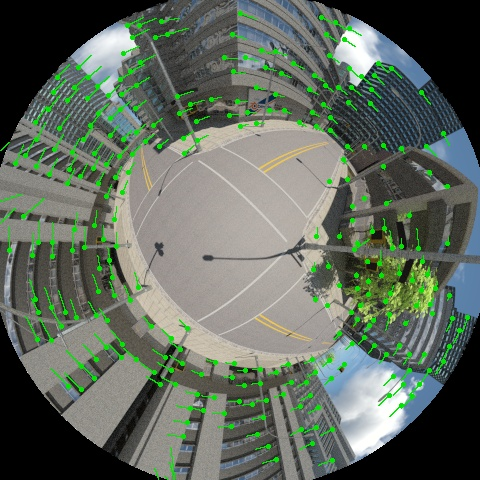
\includegraphics[width=\textwidth]{./figures/robot/method_systemstructure_features.jpg}
    \caption{Urban canyon scenario.}
    \label{fig:robot_experiments_simulation_urbancanyon}
  \end{subfigure}\hfill
  \begin{subfigure}[]{0.475\textwidth}
    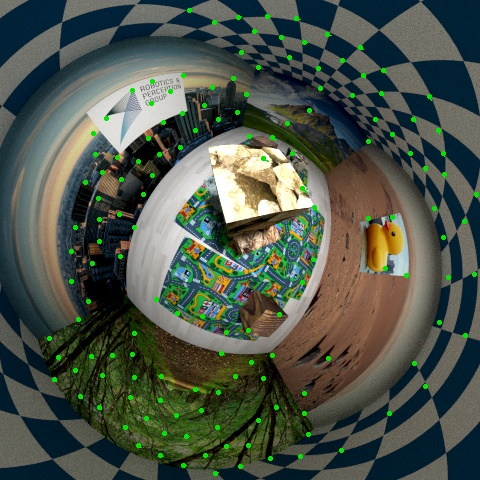
\includegraphics[width=\textwidth]{./figures/robot/indoor_features.jpg}
    \caption{Indoor scenario.}
    \label{fig:robot_experiments_simulation_indoor}
  \end{subfigure}
  \caption{Urban canyon and indoor scenario with sparse optical flow (visualized as green dots and lines).}
  \label{fig:robot_experiments_simulation}
\end{figure}

\begin{figure}[]
  \centering
  \begin{subfigure}[]{\textwidth}
    \centering
    \begin{tikzpicture}[gnuplot]
%% generated with GNUPLOT 5.2p2 (Gentoo revision r0) (Lua 5.1; terminal rev. 99, script rev. 102)
%% Wed 13 Jun 2018 09:57:15 AM CEST
\gpcolor{color=gp lt color axes}
\gpsetlinetype{gp lt axes}
\gpsetdashtype{gp dt axes}
\gpsetlinewidth{0.50}
\draw[gp path] (1.724,1.262)--(9.724,1.262);
\gpcolor{color=gp lt color border}
\gpsetlinetype{gp lt border}
\gpsetdashtype{gp dt solid}
\gpsetlinewidth{1.00}
\draw[gp path] (1.724,1.262)--(1.959,1.262);
\node[gp node right] at (1.530,1.262) {$-20$};
\gpcolor{color=gp lt color axes}
\gpsetlinetype{gp lt axes}
\gpsetdashtype{gp dt axes}
\gpsetlinewidth{0.50}
\draw[gp path] (1.724,2.737)--(9.724,2.737);
\gpcolor{color=gp lt color border}
\gpsetlinetype{gp lt border}
\gpsetdashtype{gp dt solid}
\gpsetlinewidth{1.00}
\draw[gp path] (1.724,2.737)--(1.959,2.737);
\node[gp node right] at (1.530,2.737) {$20$};
\gpcolor{color=gp lt color axes}
\gpsetlinetype{gp lt axes}
\gpsetdashtype{gp dt axes}
\gpsetlinewidth{0.50}
\draw[gp path] (1.724,4.212)--(9.724,4.212);
\gpcolor{color=gp lt color border}
\gpsetlinetype{gp lt border}
\gpsetdashtype{gp dt solid}
\gpsetlinewidth{1.00}
\draw[gp path] (1.724,4.212)--(1.959,4.212);
\node[gp node right] at (1.530,4.212) {$60$};
\gpcolor{color=gp lt color axes}
\gpsetlinetype{gp lt axes}
\gpsetdashtype{gp dt axes}
\gpsetlinewidth{0.50}
\draw[gp path] (1.724,5.687)--(9.724,5.687);
\gpcolor{color=gp lt color border}
\gpsetlinetype{gp lt border}
\gpsetdashtype{gp dt solid}
\gpsetlinewidth{1.00}
\draw[gp path] (1.724,5.687)--(1.959,5.687);
\node[gp node right] at (1.530,5.687) {$100$};
\gpcolor{color=gp lt color axes}
\gpsetlinetype{gp lt axes}
\gpsetdashtype{gp dt axes}
\gpsetlinewidth{0.50}
\draw[gp path] (1.724,7.162)--(9.724,7.162);
\gpcolor{color=gp lt color border}
\gpsetlinetype{gp lt border}
\gpsetdashtype{gp dt solid}
\gpsetlinewidth{1.00}
\draw[gp path] (1.724,7.162)--(1.959,7.162);
\node[gp node right] at (1.530,7.162) {$140$};
\gpcolor{color=gp lt color axes}
\gpsetlinetype{gp lt axes}
\gpsetdashtype{gp dt axes}
\gpsetlinewidth{0.50}
\draw[gp path] (2.451,1.262)--(2.451,7.162);
\gpcolor{color=gp lt color border}
\gpsetlinetype{gp lt border}
\gpsetdashtype{gp dt solid}
\gpsetlinewidth{1.00}
\draw[gp path] (2.451,1.262)--(2.451,1.492);
\node[gp node center] at (2.451,0.867) {$0$};
\gpcolor{color=gp lt color axes}
\gpsetlinetype{gp lt axes}
\gpsetdashtype{gp dt axes}
\gpsetlinewidth{0.50}
\draw[gp path] (3.905,1.262)--(3.905,7.162);
\gpcolor{color=gp lt color border}
\gpsetlinetype{gp lt border}
\gpsetdashtype{gp dt solid}
\gpsetlinewidth{1.00}
\draw[gp path] (3.905,1.262)--(3.905,1.492);
\node[gp node center] at (3.905,0.867) {$40$};
\gpcolor{color=gp lt color axes}
\gpsetlinetype{gp lt axes}
\gpsetdashtype{gp dt axes}
\gpsetlinewidth{0.50}
\draw[gp path] (5.360,1.262)--(5.360,7.162);
\gpcolor{color=gp lt color border}
\gpsetlinetype{gp lt border}
\gpsetdashtype{gp dt solid}
\gpsetlinewidth{1.00}
\draw[gp path] (5.360,1.262)--(5.360,1.492);
\node[gp node center] at (5.360,0.867) {$80$};
\gpcolor{color=gp lt color axes}
\gpsetlinetype{gp lt axes}
\gpsetdashtype{gp dt axes}
\gpsetlinewidth{0.50}
\draw[gp path] (6.814,1.262)--(6.814,7.162);
\gpcolor{color=gp lt color border}
\gpsetlinetype{gp lt border}
\gpsetdashtype{gp dt solid}
\gpsetlinewidth{1.00}
\draw[gp path] (6.814,1.262)--(6.814,1.492);
\node[gp node center] at (6.814,0.867) {$120$};
\gpcolor{color=gp lt color axes}
\gpsetlinetype{gp lt axes}
\gpsetdashtype{gp dt axes}
\gpsetlinewidth{0.50}
\draw[gp path] (8.269,1.262)--(8.269,7.162);
\gpcolor{color=gp lt color border}
\gpsetlinetype{gp lt border}
\gpsetdashtype{gp dt solid}
\gpsetlinewidth{1.00}
\draw[gp path] (8.269,1.262)--(8.269,1.492);
\node[gp node center] at (8.269,0.867) {$160$};
\draw[gp path] (1.724,7.162)--(1.724,1.262)--(9.724,1.262)--(9.724,7.162)--cycle;
\node[gp node center,rotate=-270] at (0.601,4.212) {y [m]};
\node[gp node center] at (5.723,0.275) {x [m]};
\gpcolor{rgb color={0.000,0.667,0.000}}
\gpsetlinewidth{3.00}
\draw[gp path] (2.451,2.000)--(2.452,2.011)--(2.453,2.023)--(2.455,2.034)--(2.455,2.044)%
  --(2.456,2.055)--(2.457,2.065)--(2.457,2.075)--(2.459,2.084)--(2.459,2.093)--(2.460,2.102)%
  --(2.460,2.111)--(2.461,2.119)--(2.463,2.128)--(2.463,2.135)--(2.464,2.143)--(2.464,2.152)%
  --(2.465,2.160)--(2.465,2.167)--(2.466,2.175)--(2.466,2.183)--(2.468,2.190)--(2.468,2.198)%
  --(2.469,2.206)--(2.470,2.213)--(2.470,2.220)--(2.470,2.228)--(2.472,2.235)--(2.473,2.242)%
  --(2.473,2.249)--(2.474,2.256)--(2.474,2.262)--(2.476,2.269)--(2.476,2.275)--(2.477,2.281)%
  --(2.477,2.288)--(2.477,2.294)--(2.478,2.301)--(2.478,2.307)--(2.478,2.312)--(2.478,2.318)%
  --(2.480,2.324)--(2.480,2.330)--(2.480,2.335)--(2.481,2.340)--(2.481,2.345)--(2.481,2.352)%
  --(2.481,2.357)--(2.481,2.363)--(2.482,2.368)--(2.482,2.375)--(2.482,2.380)--(2.483,2.386)%
  --(2.483,2.393)--(2.483,2.399)--(2.483,2.406)--(2.485,2.412)--(2.485,2.418)--(2.485,2.425)%
  --(2.485,2.431)--(2.485,2.438)--(2.485,2.445)--(2.486,2.452)--(2.486,2.458)--(2.486,2.466)%
  --(2.486,2.472)--(2.487,2.480)--(2.487,2.488)--(2.487,2.494)--(2.487,2.502)--(2.487,2.509)%
  --(2.489,2.517)--(2.489,2.525)--(2.489,2.532)--(2.489,2.539)--(2.489,2.547)--(2.489,2.553)%
  --(2.489,2.561)--(2.489,2.567)--(2.489,2.573)--(2.490,2.580)--(2.490,2.586)--(2.490,2.593)%
  --(2.490,2.599)--(2.490,2.605)--(2.490,2.612)--(2.490,2.617)--(2.490,2.623)--(2.490,2.628)%
  --(2.491,2.635)--(2.491,2.640)--(2.491,2.645)--(2.491,2.652)--(2.491,2.657)--(2.491,2.662)%
  --(2.493,2.667)--(2.493,2.671)--(2.493,2.676)--(2.493,2.681)--(2.493,2.686)--(2.493,2.690)%
  --(2.493,2.695)--(2.493,2.699)--(2.493,2.704)--(2.494,2.708)--(2.494,2.713)--(2.494,2.717)%
  --(2.494,2.722)--(2.494,2.726)--(2.494,2.731)--(2.494,2.735)--(2.494,2.740)--(2.494,2.745)%
  --(2.494,2.750)--(2.494,2.757)--(2.494,2.763)--(2.494,2.769)--(2.494,2.776)--(2.494,2.783)%
  --(2.494,2.791)--(2.494,2.799)--(2.494,2.807)--(2.494,2.814)--(2.494,2.822)--(2.494,2.828)%
  --(2.494,2.836)--(2.494,2.844)--(2.494,2.851)--(2.494,2.858)--(2.493,2.864)--(2.493,2.872)%
  --(2.493,2.878)--(2.493,2.885)--(2.493,2.891)--(2.493,2.896)--(2.493,2.903)--(2.493,2.909)%
  --(2.493,2.915)--(2.493,2.921)--(2.493,2.927)--(2.493,2.932)--(2.493,2.938)--(2.493,2.944)%
  --(2.493,2.950)--(2.493,2.955)--(2.493,2.960)--(2.493,2.965)--(2.493,2.970)--(2.493,2.976)%
  --(2.493,2.981)--(2.493,2.986)--(2.493,2.990)--(2.493,2.995)--(2.493,3.000)--(2.493,3.006)%
  --(2.491,3.011)--(2.493,3.017)--(2.491,3.022)--(2.493,3.028)--(2.493,3.035)--(2.493,3.040)%
  --(2.491,3.046)--(2.491,3.052)--(2.491,3.059)--(2.491,3.065)--(2.491,3.072)--(2.491,3.078)%
  --(2.491,3.084)--(2.491,3.092)--(2.491,3.099)--(2.490,3.106)--(2.490,3.113)--(2.490,3.120)%
  --(2.490,3.128)--(2.489,3.134)--(2.489,3.142)--(2.489,3.150)--(2.489,3.156)--(2.487,3.164)%
  --(2.487,3.170)--(2.487,3.178)--(2.487,3.184)--(2.487,3.192)--(2.486,3.199)--(2.486,3.205)%
  --(2.486,3.211)--(2.486,3.218)--(2.485,3.224)--(2.485,3.231)--(2.485,3.237)--(2.485,3.243)%
  --(2.485,3.250)--(2.483,3.255)--(2.483,3.261)--(2.483,3.266)--(2.483,3.273)--(2.483,3.278)%
  --(2.483,3.284)--(2.483,3.289)--(2.482,3.295)--(2.482,3.300)--(2.482,3.305)--(2.482,3.310)%
  --(2.482,3.315)--(2.482,3.320)--(2.482,3.325)--(2.482,3.330)--(2.482,3.336)--(2.482,3.341)%
  --(2.482,3.346)--(2.482,3.351)--(2.481,3.356)--(2.481,3.360)--(2.481,3.365)--(2.481,3.370)%
  --(2.481,3.375)--(2.481,3.379)--(2.481,3.384)--(2.481,3.389)--(2.481,3.394)--(2.481,3.401)%
  --(2.481,3.406)--(2.480,3.412)--(2.480,3.418)--(2.480,3.424)--(2.480,3.429)--(2.480,3.435)%
  --(2.480,3.442)--(2.480,3.448)--(2.480,3.455)--(2.480,3.461)--(2.478,3.467)--(2.478,3.474)%
  --(2.478,3.480)--(2.478,3.487)--(2.478,3.492)--(2.478,3.498)--(2.477,3.505)--(2.477,3.510)%
  --(2.477,3.516)--(2.477,3.521)--(2.477,3.526)--(2.477,3.533)--(2.477,3.538)--(2.477,3.543)%
  --(2.476,3.548)--(2.476,3.553)--(2.476,3.558)--(2.476,3.564)--(2.476,3.569)--(2.476,3.574)%
  --(2.476,3.579)--(2.476,3.584)--(2.476,3.588)--(2.476,3.593)--(2.476,3.598)--(2.476,3.603)%
  --(2.474,3.608)--(2.474,3.614)--(2.474,3.619)--(2.474,3.624)--(2.474,3.629)--(2.474,3.634)%
  --(2.474,3.639)--(2.474,3.643)--(2.474,3.648)--(2.473,3.653)--(2.473,3.657)--(2.473,3.662)%
  --(2.473,3.667)--(2.473,3.672)--(2.473,3.676)--(2.473,3.681)--(2.472,3.687)--(2.472,3.692)%
  --(2.472,3.697)--(2.472,3.703)--(2.472,3.708)--(2.472,3.713)--(2.472,3.720)--(2.472,3.725)%
  --(2.472,3.731)--(2.470,3.736)--(2.470,3.743)--(2.470,3.749)--(2.470,3.756)--(2.470,3.762)%
  --(2.470,3.769)--(2.470,3.775)--(2.470,3.781)--(2.469,3.788)--(2.469,3.794)--(2.469,3.801)%
  --(2.469,3.807)--(2.469,3.813)--(2.469,3.820)--(2.469,3.826)--(2.468,3.833)--(2.468,3.839)%
  --(2.468,3.845)--(2.468,3.852)--(2.468,3.858)--(2.468,3.865)--(2.468,3.871)--(2.466,3.877)%
  --(2.466,3.884)--(2.466,3.890)--(2.466,3.897)--(2.465,3.904)--(2.465,3.911)--(2.465,3.917)%
  --(2.464,3.925)--(2.464,3.932)--(2.464,3.939)--(2.463,3.947)--(2.463,3.954)--(2.463,3.962)%
  --(2.461,3.970)--(2.461,3.977)--(2.461,3.985)--(2.461,3.993)--(2.460,4.000)--(2.460,4.007)%
  --(2.460,4.014)--(2.460,4.021)--(2.460,4.029)--(2.459,4.035)--(2.459,4.043)--(2.459,4.049)%
  --(2.459,4.057)--(2.459,4.063)--(2.457,4.071)--(2.457,4.077)--(2.457,4.085)--(2.457,4.091)%
  --(2.456,4.098)--(2.456,4.105)--(2.456,4.112)--(2.456,4.119)--(2.456,4.127)--(2.456,4.135)%
  --(2.455,4.144)--(2.455,4.152)--(2.455,4.160)--(2.455,4.168)--(2.453,4.177)--(2.453,4.185)%
  --(2.453,4.194)--(2.452,4.203)--(2.452,4.210)--(2.452,4.219)--(2.452,4.228)--(2.451,4.237)%
  --(2.451,4.246)--(2.451,4.254)--(2.451,4.263)--(2.451,4.271)--(2.451,4.280)--(2.451,4.287)%
  --(2.451,4.295)--(2.449,4.303)--(2.449,4.310)--(2.449,4.318)--(2.449,4.326)--(2.449,4.333)%
  --(2.449,4.341)--(2.449,4.349)--(2.449,4.356)--(2.449,4.364)--(2.449,4.372)--(2.448,4.380)%
  --(2.449,4.387)--(2.449,4.395)--(2.449,4.403)--(2.449,4.410)--(2.449,4.418)--(2.449,4.426)%
  --(2.449,4.432)--(2.449,4.440)--(2.451,4.447)--(2.451,4.455)--(2.452,4.463)--(2.452,4.469)%
  --(2.453,4.477)--(2.455,4.485)--(2.456,4.492)--(2.457,4.500)--(2.459,4.506)--(2.460,4.514)%
  --(2.461,4.522)--(2.463,4.529)--(2.464,4.536)--(2.465,4.542)--(2.466,4.550)--(2.469,4.556)%
  --(2.472,4.563)--(2.474,4.570)--(2.477,4.577)--(2.480,4.584)--(2.482,4.591)--(2.486,4.597)%
  --(2.489,4.604)--(2.490,4.611)--(2.493,4.619)--(2.495,4.625)--(2.498,4.633)--(2.500,4.640)%
  --(2.504,4.646)--(2.508,4.654)--(2.512,4.660)--(2.517,4.666)--(2.523,4.673)--(2.528,4.679)%
  --(2.533,4.686)--(2.540,4.692)--(2.545,4.698)--(2.549,4.706)--(2.554,4.714)--(2.559,4.722)%
  --(2.566,4.729)--(2.571,4.736)--(2.577,4.743)--(2.585,4.750)--(2.592,4.756)--(2.598,4.761)%
  --(2.606,4.768)--(2.614,4.773)--(2.622,4.778)--(2.630,4.782)--(2.638,4.787)--(2.643,4.792)%
  --(2.649,4.797)--(2.656,4.802)--(2.662,4.807)--(2.669,4.811)--(2.675,4.815)--(2.682,4.820)%
  --(2.688,4.823)--(2.695,4.827)--(2.700,4.829)--(2.707,4.830)--(2.712,4.833)--(2.717,4.834)%
  --(2.724,4.837)--(2.729,4.839)--(2.734,4.842)--(2.739,4.845)--(2.746,4.847)--(2.751,4.850)%
  --(2.756,4.851)--(2.763,4.853)--(2.769,4.855)--(2.775,4.856)--(2.781,4.857)--(2.788,4.859)%
  --(2.793,4.860)--(2.799,4.861)--(2.806,4.862)--(2.812,4.864)--(2.818,4.866)--(2.826,4.868)%
  --(2.832,4.869)--(2.839,4.870)--(2.845,4.871)--(2.852,4.873)--(2.858,4.874)--(2.863,4.874)%
  --(2.870,4.875)--(2.876,4.875)--(2.883,4.877)--(2.890,4.877)--(2.896,4.878)--(2.903,4.878)%
  --(2.909,4.879)--(2.916,4.879)--(2.923,4.880)--(2.930,4.880)--(2.938,4.880)--(2.944,4.882)%
  --(2.952,4.882)--(2.959,4.882)--(2.967,4.882)--(2.973,4.882)--(2.981,4.882)--(2.989,4.882)%
  --(2.997,4.882)--(3.003,4.882)--(3.011,4.882)--(3.019,4.882)--(3.025,4.882)--(3.033,4.882)%
  --(3.040,4.882)--(3.046,4.882)--(3.053,4.882)--(3.059,4.882)--(3.067,4.880)--(3.074,4.880)%
  --(3.080,4.879)--(3.088,4.879)--(3.094,4.879)--(3.102,4.878)--(3.109,4.878)--(3.117,4.878)%
  --(3.123,4.877)--(3.130,4.877)--(3.136,4.877)--(3.143,4.875)--(3.149,4.875)--(3.157,4.875)%
  --(3.164,4.874)--(3.169,4.874)--(3.175,4.874)--(3.182,4.873)--(3.189,4.873)--(3.195,4.871)%
  --(3.202,4.871)--(3.208,4.871)--(3.215,4.870)--(3.221,4.870)--(3.228,4.870)--(3.234,4.870)%
  --(3.241,4.869)--(3.247,4.869)--(3.254,4.869)--(3.259,4.868)--(3.264,4.868)--(3.271,4.868)%
  --(3.277,4.866)--(3.284,4.866)--(3.290,4.865)--(3.297,4.865)--(3.303,4.864)--(3.310,4.862)%
  --(3.318,4.862)--(3.324,4.861)--(3.332,4.860)--(3.339,4.859)--(3.345,4.857)--(3.353,4.857)%
  --(3.360,4.856)--(3.367,4.855)--(3.375,4.853)--(3.384,4.852)--(3.392,4.851)--(3.401,4.848)%
  --(3.409,4.846)--(3.418,4.843)--(3.426,4.841)--(3.435,4.837)--(3.443,4.833)--(3.451,4.829)%
  --(3.459,4.824)--(3.467,4.819)--(3.474,4.814)--(3.482,4.810)--(3.489,4.809)--(3.495,4.806)%
  --(3.502,4.804)--(3.507,4.801)--(3.514,4.797)--(3.519,4.792)--(3.524,4.788)--(3.529,4.783)%
  --(3.535,4.777)--(3.538,4.771)--(3.542,4.765)--(3.545,4.759)--(3.549,4.752)--(3.553,4.747)%
  --(3.558,4.742)--(3.563,4.737)--(3.567,4.731)--(3.572,4.725)--(3.576,4.718)--(3.579,4.711)%
  --(3.583,4.704)--(3.585,4.697)--(3.588,4.690)--(3.589,4.681)--(3.591,4.674)--(3.591,4.666)%
  --(3.591,4.659)--(3.593,4.650)--(3.596,4.642)--(3.598,4.634)--(3.601,4.625)--(3.602,4.617)%
  --(3.604,4.606)--(3.606,4.597)--(3.608,4.587)--(3.609,4.577)--(3.610,4.568)--(3.610,4.558)%
  --(3.610,4.549)--(3.610,4.538)--(3.610,4.529)--(3.612,4.520)--(3.612,4.511)--(3.613,4.502)%
  --(3.613,4.494)--(3.613,4.485)--(3.613,4.477)--(3.613,4.468)--(3.613,4.460)--(3.613,4.453)%
  --(3.613,4.446)--(3.613,4.438)--(3.613,4.432)--(3.613,4.426)--(3.612,4.418)--(3.612,4.412)%
  --(3.612,4.404)--(3.612,4.397)--(3.610,4.391)--(3.610,4.385)--(3.610,4.378)--(3.610,4.371)%
  --(3.610,4.364)--(3.610,4.356)--(3.610,4.350)--(3.610,4.342)--(3.609,4.335)--(3.609,4.327)%
  --(3.609,4.321)--(3.609,4.313)--(3.609,4.307)--(3.609,4.300)--(3.609,4.294)--(3.610,4.287)%
  --(3.610,4.281)--(3.610,4.274)--(3.612,4.268)--(3.612,4.262)--(3.613,4.254)--(3.613,4.248)%
  --(3.614,4.241)--(3.615,4.233)--(3.617,4.226)--(3.617,4.218)--(3.618,4.210)--(3.619,4.203)%
  --(3.621,4.195)--(3.622,4.187)--(3.625,4.178)--(3.627,4.171)--(3.630,4.163)--(3.634,4.157)%
  --(3.636,4.149)--(3.640,4.141)--(3.644,4.135)--(3.648,4.128)--(3.651,4.122)--(3.652,4.116)%
  --(3.653,4.108)--(3.655,4.102)--(3.657,4.095)--(3.661,4.089)--(3.664,4.082)--(3.669,4.076)%
  --(3.674,4.071)--(3.679,4.064)--(3.685,4.059)--(3.691,4.054)--(3.698,4.050)--(3.704,4.046)%
  --(3.709,4.043)--(3.715,4.038)--(3.720,4.032)--(3.725,4.026)--(3.732,4.021)--(3.738,4.017)%
  --(3.745,4.012)--(3.751,4.008)--(3.758,4.003)--(3.766,4.000)--(3.772,3.997)--(3.780,3.993)%
  --(3.788,3.990)--(3.796,3.989)--(3.803,3.986)--(3.811,3.982)--(3.819,3.980)--(3.827,3.977)%
  --(3.835,3.973)--(3.841,3.972)--(3.849,3.970)--(3.856,3.967)--(3.864,3.966)--(3.871,3.963)%
  --(3.879,3.961)--(3.888,3.959)--(3.896,3.958)--(3.904,3.957)--(3.912,3.954)--(3.921,3.952)%
  --(3.929,3.949)--(3.937,3.948)--(3.945,3.945)--(3.952,3.944)--(3.960,3.943)--(3.968,3.941)%
  --(3.976,3.940)--(3.984,3.940)--(3.992,3.939)--(3.999,3.939)--(4.007,3.939)--(4.015,3.939)%
  --(4.023,3.938)--(4.029,3.938)--(4.036,3.936)--(4.044,3.936)--(4.052,3.936)--(4.059,3.936)%
  --(4.069,3.938)--(4.076,3.938)--(4.086,3.939)--(4.095,3.940)--(4.104,3.941)--(4.113,3.944)%
  --(4.122,3.945)--(4.131,3.948)--(4.142,3.949)--(4.151,3.950)--(4.161,3.952)--(4.170,3.953)%
  --(4.181,3.956)--(4.190,3.958)--(4.199,3.961)--(4.208,3.962)--(4.217,3.966)--(4.227,3.968)%
  --(4.234,3.971)--(4.244,3.975)--(4.253,3.980)--(4.262,3.984)--(4.271,3.986)--(4.281,3.990)%
  --(4.292,3.994)--(4.302,3.998)--(4.313,4.002)--(4.323,4.007)--(4.334,4.012)--(4.345,4.018)%
  --(4.356,4.023)--(4.365,4.030)--(4.374,4.035)--(4.382,4.040)--(4.390,4.045)--(4.398,4.052)%
  --(4.405,4.055)--(4.413,4.061)--(4.420,4.066)--(4.428,4.071)--(4.434,4.076)--(4.441,4.081)%
  --(4.447,4.086)--(4.454,4.093)--(4.459,4.098)--(4.464,4.104)--(4.469,4.111)--(4.475,4.116)%
  --(4.480,4.122)--(4.484,4.128)--(4.489,4.134)--(4.496,4.139)--(4.501,4.144)--(4.506,4.150)%
  --(4.510,4.157)--(4.515,4.163)--(4.519,4.169)--(4.523,4.176)--(4.526,4.184)--(4.528,4.191)%
  --(4.531,4.199)--(4.533,4.207)--(4.535,4.214)--(4.536,4.222)--(4.540,4.228)--(4.544,4.236)%
  --(4.546,4.242)--(4.550,4.250)--(4.553,4.258)--(4.556,4.266)--(4.558,4.273)--(4.559,4.281)%
  --(4.562,4.289)--(4.563,4.296)--(4.565,4.304)--(4.566,4.312)--(4.567,4.321)--(4.569,4.328)%
  --(4.570,4.336)--(4.573,4.345)--(4.574,4.353)--(4.575,4.360)--(4.576,4.369)--(4.578,4.377)%
  --(4.579,4.385)--(4.579,4.392)--(4.580,4.401)--(4.580,4.409)--(4.582,4.417)--(4.582,4.424)%
  --(4.580,4.432)--(4.582,4.440)--(4.582,4.447)--(4.582,4.455)--(4.582,4.464)--(4.582,4.472)%
  --(4.582,4.481)--(4.582,4.491)--(4.580,4.501)--(4.580,4.511)--(4.579,4.523)--(4.578,4.535)%
  --(4.575,4.547)--(4.574,4.560)--(4.571,4.573)--(4.570,4.586)--(4.569,4.600)--(4.567,4.613)%
  --(4.566,4.627)--(4.565,4.640)--(4.562,4.652)--(4.559,4.664)--(4.557,4.677)--(4.554,4.688)%
  --(4.552,4.700)--(4.548,4.711)--(4.545,4.723)--(4.541,4.734)--(4.539,4.745)--(4.535,4.756)%
  --(4.532,4.766)--(4.529,4.775)--(4.526,4.786)--(4.523,4.796)--(4.519,4.805)--(4.515,4.814)%
  --(4.511,4.824)--(4.507,4.833)--(4.502,4.842)--(4.498,4.851)--(4.493,4.860)--(4.488,4.869)%
  --(4.482,4.878)--(4.479,4.888)--(4.475,4.898)--(4.471,4.907)--(4.465,4.916)--(4.460,4.925)%
  --(4.455,4.933)--(4.450,4.941)--(4.445,4.947)--(4.438,4.953)--(4.432,4.960)--(4.425,4.966)%
  --(4.418,4.971)--(4.412,4.976)--(4.407,4.980)--(4.402,4.987)--(4.398,4.992)--(4.394,4.997)%
  --(4.388,5.002)--(4.383,5.007)--(4.379,5.011)--(4.374,5.015)--(4.369,5.017)--(4.362,5.021)%
  --(4.357,5.024)--(4.351,5.026)--(4.345,5.028)--(4.339,5.029)--(4.334,5.030)--(4.327,5.034)%
  --(4.322,5.037)--(4.315,5.039)--(4.310,5.042)--(4.304,5.043)--(4.297,5.046)--(4.291,5.048)%
  --(4.284,5.049)--(4.277,5.051)--(4.271,5.052)--(4.266,5.053)--(4.259,5.053)--(4.253,5.055)%
  --(4.246,5.055)--(4.240,5.056)--(4.233,5.057)--(4.227,5.057)--(4.220,5.058)--(4.212,5.060)%
  --(4.206,5.060)--(4.199,5.061)--(4.191,5.061)--(4.185,5.061)--(4.177,5.062)--(4.170,5.062)%
  --(4.164,5.062)--(4.156,5.061)--(4.148,5.061)--(4.140,5.062)--(4.134,5.062)--(4.126,5.062)%
  --(4.118,5.062)--(4.110,5.062)--(4.102,5.062)--(4.096,5.062)--(4.088,5.062)--(4.082,5.062)%
  --(4.074,5.062)--(4.066,5.061)--(4.058,5.061)--(4.050,5.060)--(4.042,5.060)--(4.036,5.058)%
  --(4.029,5.058)--(4.024,5.058)--(4.018,5.057)--(4.012,5.057)--(4.007,5.057)--(4.001,5.056)%
  --(3.994,5.056)--(3.989,5.056)--(3.982,5.055)--(3.976,5.053)--(3.969,5.053)--(3.963,5.052)%
  --(3.956,5.051)--(3.950,5.051)--(3.942,5.049)--(3.935,5.048)--(3.928,5.048)--(3.920,5.047)%
  --(3.913,5.046)--(3.905,5.044)--(3.898,5.043)--(3.890,5.042)--(3.882,5.042)--(3.874,5.040)%
  --(3.866,5.039)--(3.858,5.038)--(3.850,5.037)--(3.843,5.035)--(3.835,5.034)--(3.827,5.033)%
  --(3.818,5.032)--(3.809,5.029)--(3.800,5.028)--(3.792,5.026)--(3.783,5.024)--(3.773,5.023)%
  --(3.763,5.021)--(3.754,5.019)--(3.745,5.017)--(3.736,5.015)--(3.726,5.014)--(3.717,5.012)%
  --(3.708,5.010)--(3.698,5.008)--(3.689,5.006)--(3.679,5.005)--(3.669,5.002)--(3.660,5.001)%
  --(3.651,4.998)--(3.640,4.996)--(3.631,4.994)--(3.621,4.992)--(3.610,4.989)--(3.601,4.988)%
  --(3.591,4.985)--(3.582,4.983)--(3.571,4.982)--(3.562,4.979)--(3.553,4.978)--(3.542,4.975)%
  --(3.533,4.974)--(3.524,4.971)--(3.516,4.970)--(3.507,4.967)--(3.498,4.966)--(3.489,4.965)%
  --(3.481,4.964)--(3.473,4.961)--(3.464,4.960)--(3.456,4.959)--(3.447,4.957)--(3.438,4.955)%
  --(3.430,4.953)--(3.421,4.952)--(3.413,4.951)--(3.404,4.948)--(3.396,4.947)--(3.388,4.946)%
  --(3.379,4.944)--(3.371,4.943)--(3.363,4.942)--(3.357,4.941)--(3.349,4.938)--(3.341,4.937)%
  --(3.333,4.935)--(3.326,4.934)--(3.319,4.933)--(3.311,4.932)--(3.303,4.930)--(3.297,4.929)%
  --(3.289,4.928)--(3.281,4.926)--(3.275,4.925)--(3.267,4.924)--(3.260,4.923)--(3.252,4.921)%
  --(3.246,4.920)--(3.238,4.919)--(3.232,4.918)--(3.225,4.916)--(3.219,4.915)--(3.211,4.914)%
  --(3.204,4.912)--(3.196,4.911)--(3.189,4.910)--(3.182,4.909)--(3.174,4.907)--(3.168,4.906)%
  --(3.160,4.905)--(3.153,4.903)--(3.145,4.902)--(3.139,4.901)--(3.132,4.900)--(3.126,4.898)%
  --(3.118,4.898)--(3.111,4.897)--(3.105,4.896)--(3.098,4.894)--(3.092,4.893)--(3.085,4.893)%
  --(3.079,4.892)--(3.072,4.891)--(3.066,4.889)--(3.059,4.889)--(3.053,4.888)--(3.046,4.887)%
  --(3.040,4.885)--(3.034,4.885)--(3.028,4.884)--(3.021,4.883)--(3.015,4.882)--(3.008,4.882)%
  --(3.002,4.880)--(2.995,4.879)--(2.990,4.878)--(2.984,4.878)--(2.977,4.877)--(2.969,4.875)%
  --(2.963,4.874)--(2.956,4.873)--(2.950,4.873)--(2.943,4.871)--(2.935,4.870)--(2.929,4.870)%
  --(2.921,4.869)--(2.914,4.868)--(2.906,4.866)--(2.900,4.866)--(2.892,4.865)--(2.886,4.864)%
  --(2.878,4.864)--(2.870,4.862)--(2.862,4.861)--(2.854,4.860)--(2.846,4.859)--(2.839,4.859)%
  --(2.831,4.857)--(2.822,4.857)--(2.814,4.856)--(2.805,4.856)--(2.795,4.856)--(2.786,4.856)%
  --(2.777,4.856)--(2.769,4.855)--(2.760,4.856)--(2.751,4.855)--(2.743,4.855)--(2.734,4.855)%
  --(2.726,4.853)--(2.718,4.855)--(2.709,4.855)--(2.701,4.855)--(2.694,4.856)--(2.685,4.857)%
  --(2.677,4.859)--(2.669,4.860)--(2.661,4.861)--(2.653,4.862)--(2.645,4.865)--(2.636,4.866)%
  --(2.627,4.866)--(2.619,4.868)--(2.610,4.870)--(2.601,4.871)--(2.593,4.874)--(2.585,4.878)%
  --(2.577,4.880)--(2.570,4.884)--(2.563,4.888)--(2.557,4.892)--(2.550,4.897)--(2.543,4.902)%
  --(2.537,4.907)--(2.530,4.911)--(2.523,4.914)--(2.516,4.918)--(2.510,4.921)--(2.503,4.926)%
  --(2.496,4.932)--(2.491,4.937)--(2.486,4.943)--(2.481,4.950)--(2.477,4.956)--(2.473,4.962)%
  --(2.469,4.970)--(2.466,4.978)--(2.464,4.985)--(2.460,4.991)--(2.455,4.997)--(2.449,5.003)%
  --(2.446,5.010)--(2.442,5.016)--(2.438,5.024)--(2.435,5.030)--(2.433,5.037)--(2.430,5.044)%
  --(2.427,5.052)--(2.425,5.060)--(2.423,5.067)--(2.422,5.075)--(2.421,5.083)--(2.418,5.090)%
  --(2.416,5.098)--(2.414,5.106)--(2.412,5.114)--(2.410,5.121)--(2.408,5.129)--(2.406,5.137)%
  --(2.405,5.144)--(2.404,5.152)--(2.402,5.160)--(2.401,5.167)--(2.400,5.174)--(2.399,5.181)%
  --(2.397,5.189)--(2.396,5.195)--(2.395,5.203)--(2.393,5.210)--(2.392,5.217)--(2.391,5.224)%
  --(2.391,5.230)--(2.389,5.238)--(2.388,5.244)--(2.387,5.252)--(2.386,5.260)--(2.386,5.267)%
  --(2.384,5.275)--(2.383,5.281)--(2.383,5.289)--(2.382,5.295)--(2.380,5.303)--(2.379,5.309)%
  --(2.379,5.317)--(2.378,5.324)--(2.376,5.331)--(2.376,5.339)--(2.375,5.345)--(2.375,5.353)%
  --(2.374,5.361)--(2.374,5.368)--(2.372,5.376)--(2.372,5.384)--(2.371,5.391)--(2.370,5.398)%
  --(2.370,5.406)--(2.369,5.412)--(2.369,5.420)--(2.367,5.426)--(2.367,5.432)--(2.366,5.439)%
  --(2.366,5.445)--(2.365,5.452)--(2.365,5.458)--(2.363,5.464)--(2.363,5.471)--(2.363,5.476)%
  --(2.362,5.482)--(2.362,5.489)--(2.361,5.494)--(2.361,5.500)--(2.359,5.505)--(2.359,5.512)%
  --(2.358,5.518)--(2.358,5.523)--(2.357,5.530)--(2.357,5.535)--(2.355,5.541)--(2.355,5.548)%
  --(2.355,5.554)--(2.354,5.562)--(2.354,5.568)--(2.353,5.575)--(2.353,5.581)--(2.352,5.589)%
  --(2.352,5.596)--(2.350,5.603)--(2.350,5.611)--(2.349,5.618)--(2.349,5.625)--(2.349,5.632)%
  --(2.348,5.639)--(2.348,5.645)--(2.346,5.653)--(2.346,5.659)--(2.345,5.667)--(2.345,5.673)%
  --(2.345,5.680)--(2.344,5.686)--(2.344,5.692)--(2.342,5.699)--(2.342,5.705)--(2.342,5.712)%
  --(2.341,5.718)--(2.341,5.725)--(2.340,5.730)--(2.340,5.736)--(2.339,5.742)--(2.339,5.748)%
  --(2.339,5.753)--(2.337,5.759)--(2.337,5.764)--(2.336,5.769)--(2.336,5.776)--(2.336,5.781)%
  --(2.335,5.786)--(2.335,5.791)--(2.335,5.796)--(2.333,5.801)--(2.333,5.806)--(2.333,5.812)%
  --(2.332,5.817)--(2.332,5.822)--(2.331,5.827)--(2.331,5.831)--(2.331,5.836)--(2.329,5.841)%
  --(2.329,5.845)--(2.329,5.850)--(2.328,5.854)--(2.328,5.859)--(2.328,5.863)--(2.328,5.868)%
  --(2.327,5.872)--(2.327,5.876)--(2.327,5.881)--(2.327,5.885)--(2.325,5.890)--(2.325,5.895)%
  --(2.325,5.899)--(2.325,5.904)--(2.325,5.909)--(2.325,5.913)--(2.325,5.918)--(2.325,5.923)%
  --(2.325,5.927)--(2.325,5.932)--(2.327,5.937)--(2.327,5.942)--(2.328,5.947)--(2.328,5.953)%
  --(2.328,5.959)--(2.329,5.965)--(2.329,5.970)--(2.331,5.977)--(2.331,5.983)--(2.332,5.988)%
  --(2.335,5.995)--(2.336,6.000)--(2.337,6.006)--(2.340,6.011)--(2.342,6.018)--(2.345,6.023)%
  --(2.348,6.029)--(2.350,6.034)--(2.352,6.040)--(2.353,6.046)--(2.355,6.051)--(2.357,6.056)%
  --(2.359,6.061)--(2.362,6.067)--(2.366,6.072)--(2.369,6.077)--(2.372,6.081)--(2.376,6.086)%
  --(2.380,6.090)--(2.386,6.095)--(2.391,6.100)--(2.395,6.105)--(2.400,6.113)--(2.404,6.118)%
  --(2.408,6.125)--(2.414,6.132)--(2.419,6.138)--(2.427,6.146)--(2.435,6.155)--(2.446,6.164)%
  --(2.457,6.174)--(2.472,6.183)--(2.485,6.193)--(2.499,6.201)--(2.515,6.210)--(2.528,6.220)%
  --(2.540,6.230)--(2.551,6.239)--(2.563,6.247)--(2.572,6.255)--(2.583,6.261)--(2.593,6.268)%
  --(2.604,6.273)--(2.613,6.278)--(2.623,6.283)--(2.632,6.288)--(2.641,6.292)--(2.652,6.296)%
  --(2.660,6.298)--(2.669,6.303)--(2.677,6.307)--(2.685,6.311)--(2.692,6.315)--(2.701,6.319)%
  --(2.709,6.323)--(2.716,6.325)--(2.724,6.329)--(2.732,6.332)--(2.739,6.334)--(2.746,6.337)%
  --(2.754,6.338)--(2.762,6.341)--(2.768,6.343)--(2.776,6.344)--(2.782,6.347)--(2.790,6.351)%
  --(2.797,6.352)--(2.805,6.355)--(2.811,6.357)--(2.819,6.360)--(2.827,6.361)--(2.833,6.364)%
  --(2.841,6.365)--(2.849,6.368)--(2.857,6.369)--(2.865,6.370)--(2.873,6.373)--(2.879,6.374)%
  --(2.887,6.375)--(2.895,6.378)--(2.903,6.379)--(2.909,6.380)--(2.917,6.382)--(2.923,6.383)%
  --(2.931,6.384)--(2.938,6.385)--(2.946,6.387)--(2.952,6.388)--(2.959,6.389)--(2.965,6.389)%
  --(2.973,6.391)--(2.980,6.392)--(2.986,6.393)--(2.993,6.394)--(2.999,6.394)--(3.006,6.396)%
  --(3.012,6.397)--(3.019,6.398)--(3.024,6.398)--(3.031,6.400)--(3.037,6.400)--(3.044,6.401)%
  --(3.049,6.402)--(3.055,6.402)--(3.062,6.403)--(3.067,6.403)--(3.074,6.405)--(3.080,6.406)%
  --(3.085,6.406)--(3.092,6.407)--(3.098,6.409)--(3.105,6.409)--(3.111,6.410)--(3.118,6.410)%
  --(3.125,6.411)--(3.132,6.412)--(3.140,6.412)--(3.148,6.414)--(3.156,6.415)--(3.164,6.415)%
  --(3.172,6.416)--(3.179,6.417)--(3.189,6.419)--(3.196,6.419)--(3.205,6.420)--(3.215,6.421)%
  --(3.222,6.421)--(3.232,6.423)--(3.239,6.423)--(3.249,6.424)--(3.256,6.424)--(3.264,6.424)%
  --(3.272,6.425)--(3.280,6.425)--(3.288,6.426)--(3.296,6.426)--(3.303,6.428)--(3.310,6.428)%
  --(3.318,6.429)--(3.324,6.430)--(3.332,6.430)--(3.339,6.432)--(3.345,6.432)--(3.353,6.433)%
  --(3.360,6.434)--(3.366,6.434)--(3.373,6.435)--(3.379,6.435)--(3.386,6.437)--(3.392,6.437)%
  --(3.397,6.438)--(3.404,6.438)--(3.410,6.439)--(3.417,6.441)--(3.422,6.441)--(3.429,6.442)%
  --(3.435,6.442)--(3.441,6.443)--(3.447,6.444)--(3.452,6.444)--(3.459,6.446)--(3.465,6.447)%
  --(3.471,6.447)--(3.477,6.448)--(3.484,6.450)--(3.489,6.450)--(3.495,6.451)--(3.502,6.452)%
  --(3.507,6.453)--(3.514,6.453)--(3.519,6.455)--(3.525,6.456)--(3.531,6.456)--(3.536,6.457)%
  --(3.541,6.458)--(3.548,6.458)--(3.553,6.460)--(3.559,6.461)--(3.567,6.462)--(3.574,6.462)%
  --(3.580,6.464)--(3.587,6.465)--(3.595,6.466)--(3.601,6.467)--(3.608,6.469)--(3.614,6.470)%
  --(3.621,6.471)--(3.627,6.473)--(3.634,6.473)--(3.640,6.474)--(3.647,6.475)--(3.653,6.476)%
  --(3.660,6.478)--(3.666,6.479)--(3.672,6.480)--(3.678,6.482)--(3.683,6.482)--(3.690,6.483)%
  --(3.695,6.484)--(3.702,6.485)--(3.707,6.487)--(3.712,6.487)--(3.717,6.488)--(3.723,6.489)%
  --(3.729,6.489)--(3.734,6.491)--(3.740,6.492)--(3.745,6.493)--(3.750,6.494)--(3.755,6.494)%
  --(3.760,6.496)--(3.766,6.497)--(3.771,6.498)--(3.776,6.499)--(3.783,6.499)--(3.788,6.501)%
  --(3.794,6.502)--(3.801,6.503)--(3.806,6.503)--(3.813,6.505)--(3.819,6.506)--(3.826,6.506)%
  --(3.831,6.507)--(3.837,6.507)--(3.844,6.508)--(3.849,6.508)--(3.856,6.508)--(3.862,6.510)%
  --(3.869,6.510)--(3.875,6.511)--(3.882,6.512)--(3.888,6.512)--(3.896,6.514)--(3.903,6.514)%
  --(3.911,6.514)--(3.918,6.514)--(3.925,6.514)--(3.933,6.514)--(3.941,6.512)--(3.947,6.512)%
  --(3.954,6.511)--(3.960,6.511)--(3.967,6.510)--(3.973,6.508)--(3.980,6.508)--(3.986,6.508)%
  --(3.993,6.507)--(3.999,6.506)--(4.006,6.505)--(4.012,6.503)--(4.019,6.501)--(4.024,6.499)%
  --(4.029,6.497)--(4.033,6.494)--(4.039,6.492)--(4.042,6.489)--(4.048,6.487)--(4.053,6.484)%
  --(4.057,6.483)--(4.062,6.480)--(4.067,6.479)--(4.072,6.476)--(4.076,6.474)--(4.082,6.471)%
  --(4.086,6.467)--(4.091,6.464)--(4.095,6.460)--(4.099,6.456)--(4.102,6.451)--(4.106,6.447)%
  --(4.109,6.442)--(4.112,6.438)--(4.117,6.434)--(4.121,6.430)--(4.125,6.425)--(4.129,6.421)%
  --(4.133,6.416)--(4.136,6.411)--(4.140,6.406)--(4.143,6.401)--(4.146,6.394)--(4.150,6.388)%
  --(4.152,6.382)--(4.155,6.374)--(4.156,6.368)--(4.159,6.361)--(4.163,6.355)--(4.165,6.350)%
  --(4.168,6.343)--(4.170,6.337)--(4.173,6.330)--(4.176,6.323)--(4.178,6.316)--(4.181,6.310)%
  --(4.182,6.302)--(4.185,6.295)--(4.186,6.288)--(4.187,6.282)--(4.189,6.274)--(4.190,6.268)%
  --(4.191,6.261)--(4.193,6.255)--(4.194,6.247)--(4.197,6.241)--(4.198,6.234)--(4.199,6.227)%
  --(4.199,6.220)--(4.200,6.213)--(4.202,6.206)--(4.203,6.198)--(4.204,6.192)--(4.204,6.184)%
  --(4.206,6.177)--(4.206,6.169)--(4.207,6.163)--(4.208,6.155)--(4.208,6.149)--(4.210,6.141)%
  --(4.210,6.134)--(4.211,6.127)--(4.211,6.120)--(4.212,6.113)--(4.212,6.106)--(4.212,6.099)%
  --(4.213,6.092)--(4.213,6.084)--(4.213,6.078)--(4.215,6.072)--(4.215,6.065)--(4.215,6.059)%
  --(4.216,6.052)--(4.216,6.047)--(4.216,6.041)--(4.217,6.034)--(4.217,6.029)--(4.217,6.023)%
  --(4.219,6.018)--(4.219,6.013)--(4.219,6.006)--(4.220,6.001)--(4.220,5.996)--(4.220,5.991)%
  --(4.221,5.986)--(4.221,5.982)--(4.221,5.977)--(4.223,5.972)--(4.223,5.967)--(4.224,5.963)%
  --(4.224,5.958)--(4.225,5.953)--(4.225,5.947)--(4.227,5.942)--(4.227,5.937)--(4.228,5.932)%
  --(4.228,5.927)--(4.229,5.922)--(4.229,5.917)--(4.230,5.912)--(4.230,5.906)--(4.232,5.901)%
  --(4.232,5.896)--(4.232,5.891)--(4.233,5.886)--(4.233,5.881)--(4.234,5.876)--(4.234,5.871)%
  --(4.236,5.865)--(4.237,5.860)--(4.237,5.856)--(4.238,5.851)--(4.238,5.846)--(4.240,5.841)%
  --(4.240,5.836)--(4.241,5.831)--(4.242,5.826)--(4.242,5.819)--(4.244,5.813)--(4.245,5.806)%
  --(4.246,5.800)--(4.247,5.794)--(4.249,5.787)--(4.249,5.780)--(4.250,5.773)--(4.251,5.767)%
  --(4.253,5.760)--(4.254,5.753)--(4.255,5.746)--(4.257,5.740)--(4.258,5.733)--(4.259,5.727)%
  --(4.259,5.721)--(4.260,5.714)--(4.262,5.708)--(4.263,5.701)--(4.263,5.696)--(4.264,5.690)%
  --(4.266,5.684)--(4.266,5.678)--(4.267,5.672)--(4.268,5.667)--(4.268,5.662)--(4.270,5.655)%
  --(4.271,5.650)--(4.271,5.645)--(4.272,5.640)--(4.272,5.634)--(4.274,5.628)--(4.275,5.623)%
  --(4.275,5.617)--(4.276,5.612)--(4.276,5.605)--(4.277,5.599)--(4.279,5.593)--(4.279,5.586)%
  --(4.280,5.580)--(4.281,5.573)--(4.281,5.566)--(4.283,5.558)--(4.284,5.552)--(4.285,5.544)%
  --(4.287,5.536)--(4.288,5.529)--(4.288,5.521)--(4.289,5.514)--(4.291,5.508)--(4.292,5.500)%
  --(4.293,5.494)--(4.294,5.486)--(4.294,5.480)--(4.296,5.473)--(4.297,5.467)--(4.297,5.461)%
  --(4.298,5.456)--(4.298,5.449)--(4.300,5.443)--(4.300,5.438)--(4.301,5.431)--(4.301,5.425)%
  --(4.302,5.418)--(4.302,5.413)--(4.304,5.407)--(4.304,5.402)--(4.305,5.395)--(4.305,5.390)%
  --(4.306,5.384)--(4.306,5.379)--(4.307,5.372)--(4.307,5.367)--(4.309,5.361)--(4.309,5.354)%
  --(4.310,5.349)--(4.310,5.343)--(4.311,5.336)--(4.313,5.330)--(4.313,5.322)--(4.314,5.316)%
  --(4.315,5.308)--(4.315,5.301)--(4.317,5.294)--(4.318,5.286)--(4.319,5.279)--(4.319,5.272)%
  --(4.321,5.265)--(4.322,5.257)--(4.323,5.251)--(4.323,5.243)--(4.324,5.235)--(4.326,5.228)%
  --(4.327,5.220)--(4.328,5.212)--(4.328,5.204)--(4.330,5.197)--(4.331,5.189)--(4.332,5.181)%
  --(4.334,5.174)--(4.334,5.166)--(4.335,5.158)--(4.336,5.151)--(4.338,5.143)--(4.338,5.135)%
  --(4.339,5.128)--(4.340,5.121)--(4.341,5.114)--(4.343,5.106)--(4.343,5.098)--(4.344,5.090)%
  --(4.345,5.083)--(4.347,5.075)--(4.348,5.067)--(4.349,5.060)--(4.349,5.052)--(4.351,5.044)%
  --(4.352,5.037)--(4.353,5.029)--(4.354,5.021)--(4.356,5.014)--(4.357,5.005)--(4.357,4.997)%
  --(4.358,4.989)--(4.360,4.980)--(4.361,4.973)--(4.362,4.965)--(4.364,4.956)--(4.365,4.948)%
  --(4.365,4.941)--(4.366,4.932)--(4.368,4.924)--(4.369,4.916)--(4.370,4.909)--(4.371,4.901)%
  --(4.371,4.893)--(4.373,4.885)--(4.374,4.878)--(4.375,4.870)--(4.375,4.862)--(4.377,4.855)%
  --(4.378,4.847)--(4.379,4.839)--(4.379,4.832)--(4.381,4.824)--(4.382,4.816)--(4.382,4.809)%
  --(4.383,4.801)--(4.385,4.793)--(4.386,4.786)--(4.386,4.777)--(4.387,4.769)--(4.388,4.761)%
  --(4.390,4.754)--(4.391,4.745)--(4.392,4.737)--(4.392,4.728)--(4.394,4.720)--(4.395,4.711)%
  --(4.396,4.704)--(4.398,4.696)--(4.399,4.688)--(4.400,4.679)--(4.402,4.672)--(4.403,4.664)%
  --(4.404,4.656)--(4.405,4.649)--(4.407,4.641)--(4.408,4.633)--(4.409,4.627)--(4.409,4.619)%
  --(4.411,4.611)--(4.412,4.604)--(4.413,4.596)--(4.415,4.587)--(4.416,4.579)--(4.417,4.570)%
  --(4.417,4.563)--(4.418,4.554)--(4.420,4.545)--(4.421,4.537)--(4.422,4.528)--(4.424,4.520)%
  --(4.425,4.511)--(4.426,4.502)--(4.428,4.495)--(4.429,4.486)--(4.430,4.478)--(4.432,4.469)%
  --(4.433,4.462)--(4.434,4.453)--(4.435,4.445)--(4.437,4.436)--(4.438,4.428)--(4.439,4.421)%
  --(4.441,4.412)--(4.442,4.404)--(4.443,4.396)--(4.445,4.388)--(4.446,4.381)--(4.447,4.373)%
  --(4.449,4.365)--(4.450,4.356)--(4.450,4.349)--(4.451,4.341)--(4.452,4.332)--(4.454,4.324)%
  --(4.455,4.317)--(4.456,4.308)--(4.458,4.300)--(4.459,4.292)--(4.460,4.283)--(4.463,4.276)%
  --(4.464,4.268)--(4.464,4.260)--(4.465,4.253)--(4.467,4.245)--(4.468,4.237)--(4.469,4.230)%
  --(4.471,4.222)--(4.472,4.214)--(4.473,4.207)--(4.475,4.199)--(4.476,4.191)--(4.477,4.185)%
  --(4.479,4.177)--(4.480,4.169)--(4.481,4.162)--(4.481,4.155)--(4.482,4.148)--(4.484,4.140)%
  --(4.485,4.132)--(4.486,4.125)--(4.488,4.117)--(4.489,4.109)--(4.490,4.103)--(4.492,4.095)%
  --(4.492,4.087)--(4.493,4.081)--(4.494,4.073)--(4.496,4.066)--(4.497,4.059)--(4.498,4.052)%
  --(4.499,4.044)--(4.501,4.038)--(4.502,4.030)--(4.503,4.022)--(4.505,4.016)--(4.506,4.008)%
  --(4.507,4.000)--(4.509,3.993)--(4.510,3.986)--(4.511,3.979)--(4.512,3.971)--(4.514,3.963)%
  --(4.515,3.956)--(4.516,3.948)--(4.518,3.941)--(4.519,3.934)--(4.520,3.926)--(4.522,3.917)%
  --(4.524,3.909)--(4.526,3.902)--(4.527,3.893)--(4.528,3.885)--(4.529,3.877)--(4.531,3.870)%
  --(4.532,3.862)--(4.533,3.854)--(4.535,3.847)--(4.536,3.839)--(4.537,3.831)--(4.539,3.824)%
  --(4.540,3.817)--(4.541,3.810)--(4.543,3.802)--(4.544,3.794)--(4.545,3.788)--(4.546,3.780)%
  --(4.546,3.774)--(4.548,3.766)--(4.549,3.760)--(4.550,3.752)--(4.552,3.745)--(4.553,3.738)%
  --(4.554,3.731)--(4.556,3.724)--(4.557,3.717)--(4.558,3.711)--(4.559,3.703)--(4.561,3.697)%
  --(4.562,3.690)--(4.565,3.683)--(4.566,3.676)--(4.567,3.670)--(4.569,3.663)--(4.570,3.656)%
  --(4.573,3.649)--(4.574,3.643)--(4.575,3.637)--(4.578,3.629)--(4.579,3.622)--(4.580,3.616)%
  --(4.583,3.610)--(4.584,3.602)--(4.587,3.596)--(4.588,3.589)--(4.591,3.582)--(4.593,3.575)%
  --(4.596,3.569)--(4.597,3.562)--(4.600,3.555)--(4.603,3.548)--(4.605,3.541)--(4.608,3.534)%
  --(4.610,3.526)--(4.613,3.520)--(4.616,3.514)--(4.618,3.507)--(4.621,3.501)--(4.625,3.494)%
  --(4.627,3.488)--(4.631,3.482)--(4.634,3.475)--(4.638,3.470)--(4.642,3.464)--(4.644,3.457)%
  --(4.648,3.451)--(4.651,3.443)--(4.654,3.437)--(4.657,3.429)--(4.660,3.423)--(4.664,3.416)%
  --(4.669,3.410)--(4.673,3.403)--(4.677,3.397)--(4.682,3.391)--(4.687,3.386)--(4.693,3.379)%
  --(4.698,3.374)--(4.703,3.369)--(4.708,3.361)--(4.714,3.353)--(4.719,3.346)--(4.724,3.339)%
  --(4.731,3.333)--(4.737,3.327)--(4.744,3.320)--(4.751,3.315)--(4.759,3.309)--(4.766,3.304)%
  --(4.774,3.298)--(4.781,3.295)--(4.789,3.291)--(4.798,3.287)--(4.805,3.280)--(4.813,3.275)%
  --(4.819,3.269)--(4.827,3.265)--(4.834,3.261)--(4.842,3.257)--(4.849,3.254)--(4.856,3.251)%
  --(4.864,3.248)--(4.872,3.247)--(4.878,3.245)--(4.886,3.245)--(4.892,3.243)--(4.902,3.242)%
  --(4.909,3.239)--(4.919,3.237)--(4.926,3.234)--(4.934,3.233)--(4.942,3.232)--(4.950,3.231)%
  --(4.958,3.229)--(4.967,3.229)--(4.976,3.229)--(4.985,3.229)--(4.996,3.229)--(5.006,3.229)%
  --(5.016,3.231)--(5.026,3.232)--(5.037,3.232)--(5.047,3.232)--(5.057,3.232)--(5.066,3.232)%
  --(5.077,3.233)--(5.086,3.233)--(5.096,3.234)--(5.105,3.236)--(5.116,3.237)--(5.125,3.238)%
  --(5.135,3.241)--(5.143,3.242)--(5.152,3.245)--(5.163,3.247)--(5.172,3.248)--(5.181,3.250)%
  --(5.190,3.251)--(5.199,3.254)--(5.208,3.255)--(5.218,3.257)--(5.227,3.260)--(5.233,3.261)%
  --(5.241,3.264)--(5.249,3.265)--(5.255,3.268)--(5.263,3.270)--(5.270,3.272)--(5.275,3.274)%
  --(5.280,3.275)--(5.285,3.277)--(5.292,3.278)--(5.297,3.280)--(5.304,3.282)--(5.310,3.284)%
  --(5.317,3.286)--(5.322,3.288)--(5.329,3.291)--(5.335,3.292)--(5.342,3.295)--(5.348,3.297)%
  --(5.355,3.300)--(5.361,3.302)--(5.368,3.304)--(5.373,3.306)--(5.379,3.307)--(5.385,3.310)%
  --(5.390,3.311)--(5.396,3.314)--(5.402,3.316)--(5.408,3.319)--(5.415,3.320)--(5.420,3.323)%
  --(5.426,3.325)--(5.433,3.328)--(5.440,3.330)--(5.446,3.333)--(5.453,3.336)--(5.459,3.338)%
  --(5.466,3.341)--(5.472,3.343)--(5.479,3.346)--(5.485,3.348)--(5.492,3.351)--(5.498,3.353)%
  --(5.506,3.356)--(5.514,3.359)--(5.520,3.362)--(5.528,3.365)--(5.535,3.368)--(5.543,3.370)%
  --(5.551,3.374)--(5.557,3.377)--(5.564,3.379)--(5.571,3.382)--(5.578,3.384)--(5.586,3.387)%
  --(5.592,3.389)--(5.600,3.393)--(5.607,3.396)--(5.613,3.398)--(5.621,3.401)--(5.628,3.403)%
  --(5.634,3.406)--(5.641,3.407)--(5.647,3.410)--(5.652,3.412)--(5.659,3.415)--(5.665,3.418)%
  --(5.672,3.419)--(5.677,3.421)--(5.684,3.424)--(5.690,3.427)--(5.697,3.429)--(5.705,3.430)%
  --(5.711,3.433)--(5.718,3.435)--(5.725,3.438)--(5.732,3.441)--(5.740,3.443)--(5.746,3.446)%
  --(5.754,3.450)--(5.763,3.452)--(5.771,3.455)--(5.780,3.457)--(5.789,3.460)--(5.797,3.462)%
  --(5.808,3.466)--(5.817,3.469)--(5.826,3.471)--(5.835,3.474)--(5.846,3.476)--(5.855,3.480)%
  --(5.864,3.483)--(5.873,3.485)--(5.883,3.489)--(5.893,3.492)--(5.902,3.494)--(5.911,3.497)%
  --(5.920,3.500)--(5.929,3.502)--(5.938,3.505)--(5.947,3.507)--(5.957,3.510)--(5.966,3.512)%
  --(5.976,3.515)--(5.985,3.517)--(5.996,3.520)--(6.005,3.523)--(6.015,3.525)--(6.024,3.528)%
  --(6.035,3.530)--(6.044,3.532)--(6.053,3.534)--(6.064,3.537)--(6.073,3.538)--(6.082,3.541)%
  --(6.091,3.542)--(6.100,3.544)--(6.109,3.546)--(6.118,3.548)--(6.128,3.549)--(6.137,3.552)%
  --(6.146,3.555)--(6.154,3.556)--(6.163,3.558)--(6.172,3.560)--(6.180,3.562)--(6.189,3.564)%
  --(6.198,3.565)--(6.206,3.567)--(6.215,3.569)--(6.223,3.570)--(6.232,3.573)--(6.240,3.574)%
  --(6.249,3.575)--(6.257,3.578)--(6.266,3.579)--(6.274,3.580)--(6.282,3.583)--(6.291,3.584)%
  --(6.299,3.587)--(6.308,3.588)--(6.316,3.589)--(6.325,3.592)--(6.333,3.593)--(6.342,3.594)%
  --(6.350,3.597)--(6.359,3.598)--(6.367,3.601)--(6.376,3.602)--(6.385,3.603)--(6.394,3.606)%
  --(6.403,3.607)--(6.412,3.608)--(6.421,3.611)--(6.431,3.612)--(6.440,3.615)--(6.449,3.616)%
  --(6.459,3.617)--(6.468,3.620)--(6.479,3.621)--(6.488,3.624)--(6.497,3.625)--(6.508,3.628)%
  --(6.517,3.629)--(6.526,3.630)--(6.535,3.633)--(6.544,3.634)--(6.553,3.635)--(6.562,3.638)%
  --(6.572,3.639)--(6.579,3.640)--(6.589,3.642)--(6.598,3.644)--(6.606,3.646)--(6.615,3.647)%
  --(6.622,3.648)--(6.632,3.649)--(6.639,3.651)--(6.647,3.652)--(6.656,3.653)--(6.664,3.655)%
  --(6.672,3.656)--(6.679,3.657)--(6.686,3.658)--(6.694,3.660)--(6.701,3.661)--(6.709,3.662)%
  --(6.715,3.663)--(6.723,3.665)--(6.730,3.666)--(6.736,3.667)--(6.743,3.669)--(6.749,3.670)%
  --(6.756,3.671)--(6.762,3.672)--(6.767,3.674)--(6.774,3.675)--(6.780,3.676)--(6.787,3.678)%
  --(6.794,3.679)--(6.800,3.679)--(6.807,3.680)--(6.812,3.681)--(6.818,3.683)--(6.825,3.684)%
  --(6.831,3.685)--(6.837,3.687)--(6.843,3.687)--(6.850,3.688)--(6.856,3.689)--(6.864,3.690)%
  --(6.871,3.692)--(6.878,3.693)--(6.886,3.694)--(6.894,3.696)--(6.902,3.698)--(6.911,3.699)%
  --(6.919,3.701)--(6.927,3.702)--(6.936,3.703)--(6.942,3.704)--(6.950,3.706)--(6.958,3.707)%
  --(6.965,3.710)--(6.972,3.710)--(6.979,3.711)--(6.987,3.712)--(6.993,3.713)--(7.000,3.715)%
  --(7.008,3.716)--(7.014,3.717)--(7.021,3.719)--(7.029,3.720)--(7.035,3.720)--(7.042,3.721)%
  --(7.048,3.722)--(7.053,3.724)--(7.060,3.725)--(7.066,3.726)--(7.072,3.728)--(7.078,3.728)%
  --(7.085,3.729)--(7.091,3.730)--(7.098,3.731)--(7.104,3.733)--(7.111,3.733)--(7.117,3.734)%
  --(7.124,3.735)--(7.132,3.736)--(7.138,3.738)--(7.145,3.739)--(7.151,3.740)--(7.158,3.740)%
  --(7.166,3.742)--(7.172,3.743)--(7.180,3.744)--(7.187,3.745)--(7.194,3.747)--(7.201,3.748)%
  --(7.207,3.748)--(7.215,3.749)--(7.223,3.751)--(7.231,3.752)--(7.240,3.753)--(7.248,3.754)%
  --(7.256,3.756)--(7.265,3.758)--(7.273,3.760)--(7.281,3.761)--(7.290,3.762)--(7.298,3.763)%
  --(7.305,3.765)--(7.313,3.766)--(7.322,3.767)--(7.330,3.769)--(7.338,3.771)--(7.345,3.772)%
  --(7.352,3.774)--(7.360,3.775)--(7.368,3.776)--(7.376,3.779)--(7.382,3.780)--(7.390,3.781)%
  --(7.398,3.783)--(7.405,3.784)--(7.411,3.785)--(7.419,3.786)--(7.425,3.788)--(7.432,3.789)%
  --(7.439,3.790)--(7.446,3.792)--(7.453,3.793)--(7.459,3.793)--(7.466,3.794)--(7.472,3.795)%
  --(7.479,3.797)--(7.486,3.798)--(7.491,3.799)--(7.497,3.799)--(7.504,3.801)--(7.509,3.802)%
  --(7.516,3.803)--(7.522,3.803)--(7.527,3.804)--(7.534,3.806)--(7.539,3.806)--(7.546,3.807)%
  --(7.551,3.808)--(7.557,3.808)--(7.563,3.810)--(7.569,3.810)--(7.576,3.811)--(7.582,3.812)%
  --(7.587,3.812)--(7.594,3.813)--(7.600,3.813)--(7.607,3.815)--(7.614,3.815)--(7.620,3.815)%
  --(7.627,3.815)--(7.633,3.815)--(7.640,3.815)--(7.645,3.815)--(7.651,3.815)--(7.658,3.815)%
  --(7.664,3.815)--(7.671,3.815)--(7.676,3.815)--(7.683,3.815)--(7.689,3.815)--(7.696,3.813)%
  --(7.702,3.812)--(7.708,3.812)--(7.714,3.811)--(7.721,3.810)--(7.727,3.808)--(7.734,3.806)%
  --(7.740,3.804)--(7.747,3.802)--(7.753,3.799)--(7.760,3.799)--(7.768,3.798)--(7.775,3.797)%
  --(7.783,3.794)--(7.791,3.792)--(7.800,3.788)--(7.809,3.784)--(7.817,3.779)--(7.826,3.774)%
  --(7.834,3.769)--(7.842,3.763)--(7.850,3.757)--(7.856,3.749)--(7.864,3.744)--(7.872,3.740)%
  --(7.881,3.735)--(7.888,3.730)--(7.896,3.725)--(7.902,3.720)--(7.910,3.713)--(7.916,3.707)%
  --(7.922,3.701)--(7.928,3.694)--(7.933,3.687)--(7.937,3.679)--(7.941,3.672)--(7.945,3.665)%
  --(7.949,3.657)--(7.954,3.652)--(7.958,3.646)--(7.963,3.639)--(7.966,3.633)--(7.970,3.628)%
  --(7.974,3.621)--(7.976,3.615)--(7.980,3.607)--(7.983,3.601)--(7.986,3.594)--(7.988,3.587)%
  --(7.990,3.580)--(7.992,3.573)--(7.995,3.565)--(7.997,3.557)--(8.000,3.549)--(8.003,3.542)%
  --(8.005,3.534)--(8.008,3.526)--(8.009,3.519)--(8.012,3.512)--(8.013,3.505)--(8.016,3.497)%
  --(8.017,3.489)--(8.018,3.482)--(8.021,3.473)--(8.022,3.464)--(8.024,3.456)--(8.026,3.447)%
  --(8.027,3.437)--(8.030,3.428)--(8.033,3.418)--(8.034,3.407)--(8.037,3.397)--(8.039,3.387)%
  --(8.040,3.377)--(8.043,3.368)--(8.044,3.357)--(8.047,3.348)--(8.048,3.338)--(8.051,3.329)%
  --(8.052,3.323)--(8.054,3.316)--(8.054,3.310)--(8.055,3.304)--(8.055,3.297)--(8.055,3.291)%
  --(8.056,3.284)--(8.055,3.277)--(8.055,3.270)--(8.055,3.264)--(8.054,3.257)--(8.054,3.251)%
  --(8.052,3.245)--(8.051,3.237)--(8.051,3.232)--(8.051,3.225)--(8.051,3.219)--(8.050,3.214)%
  --(8.048,3.207)--(8.046,3.202)--(8.043,3.197)--(8.042,3.191)--(8.038,3.186)--(8.034,3.181)%
  --(8.030,3.174)--(8.025,3.169);
\gpcolor{rgb color={0.000,0.000,0.667}}
\draw[gp path] (2.451,2.000)--(2.451,2.006)--(2.452,2.014)--(2.452,2.020)--(2.453,2.028)%
  --(2.453,2.034)--(2.455,2.042)--(2.455,2.050)--(2.455,2.056)--(2.456,2.064)--(2.456,2.070)%
  --(2.457,2.076)--(2.457,2.084)--(2.457,2.092)--(2.459,2.098)--(2.459,2.106)--(2.460,2.112)%
  --(2.461,2.119)--(2.461,2.126)--(2.461,2.134)--(2.463,2.142)--(2.463,2.148)--(2.463,2.156)%
  --(2.464,2.162)--(2.464,2.170)--(2.465,2.178)--(2.465,2.184)--(2.465,2.192)--(2.466,2.199)%
  --(2.466,2.206)--(2.468,2.213)--(2.468,2.220)--(2.468,2.228)--(2.468,2.234)--(2.469,2.242)%
  --(2.469,2.248)--(2.470,2.256)--(2.470,2.262)--(2.472,2.270)--(2.472,2.276)--(2.472,2.284)%
  --(2.472,2.290)--(2.472,2.298)--(2.473,2.306)--(2.473,2.312)--(2.473,2.320)--(2.474,2.326)%
  --(2.474,2.334)--(2.474,2.340)--(2.476,2.348)--(2.476,2.356)--(2.476,2.362)--(2.476,2.370)%
  --(2.476,2.376)--(2.477,2.384)--(2.477,2.390)--(2.477,2.398)--(2.477,2.404)--(2.478,2.412)%
  --(2.478,2.420)--(2.478,2.426)--(2.478,2.434)--(2.480,2.440)--(2.480,2.448)--(2.480,2.454)%
  --(2.480,2.462)--(2.481,2.470)--(2.481,2.476)--(2.481,2.484)--(2.481,2.490)--(2.481,2.498)%
  --(2.482,2.504)--(2.482,2.512)--(2.482,2.518)--(2.482,2.526)--(2.482,2.534)--(2.482,2.540)%
  --(2.482,2.548)--(2.483,2.554)--(2.483,2.562)--(2.483,2.570)--(2.483,2.576)--(2.483,2.582)%
  --(2.485,2.590)--(2.483,2.598)--(2.485,2.604)--(2.485,2.612)--(2.485,2.618)--(2.485,2.626)%
  --(2.485,2.634)--(2.486,2.640)--(2.486,2.648)--(2.486,2.654)--(2.486,2.662)--(2.486,2.668)%
  --(2.486,2.676)--(2.486,2.684)--(2.486,2.690)--(2.487,2.698)--(2.487,2.705)--(2.487,2.712)%
  --(2.489,2.719)--(2.489,2.726)--(2.489,2.734)--(2.489,2.741)--(2.489,2.748)--(2.489,2.755)%
  --(2.489,2.762)--(2.489,2.769)--(2.490,2.776)--(2.490,2.783)--(2.489,2.791)--(2.490,2.798)%
  --(2.489,2.805)--(2.490,2.812)--(2.490,2.819)--(2.490,2.827)--(2.490,2.833)--(2.490,2.841)%
  --(2.490,2.849)--(2.490,2.856)--(2.490,2.863)--(2.490,2.869)--(2.490,2.877)--(2.490,2.885)%
  --(2.490,2.891)--(2.491,2.899)--(2.490,2.906)--(2.490,2.914)--(2.490,2.921)--(2.490,2.927)%
  --(2.490,2.935)--(2.490,2.942)--(2.490,2.949)--(2.491,2.956)--(2.491,2.963)--(2.491,2.970)%
  --(2.491,2.978)--(2.491,2.985)--(2.491,2.992)--(2.491,2.999)--(2.491,3.006)--(2.491,3.014)%
  --(2.491,3.020)--(2.491,3.028)--(2.491,3.035)--(2.491,3.042)--(2.491,3.050)--(2.491,3.056)%
  --(2.491,3.063)--(2.491,3.070)--(2.491,3.078)--(2.491,3.084)--(2.491,3.092)--(2.491,3.099)%
  --(2.491,3.106)--(2.491,3.113)--(2.491,3.120)--(2.491,3.128)--(2.491,3.134)--(2.491,3.142)%
  --(2.491,3.149)--(2.491,3.156)--(2.491,3.163)--(2.491,3.170)--(2.491,3.178)--(2.491,3.184)%
  --(2.491,3.192)--(2.490,3.200)--(2.491,3.206)--(2.491,3.214)--(2.491,3.220)--(2.491,3.228)%
  --(2.491,3.234)--(2.491,3.242)--(2.491,3.250)--(2.490,3.256)--(2.491,3.264)--(2.491,3.270)%
  --(2.490,3.278)--(2.490,3.286)--(2.491,3.293)--(2.490,3.301)--(2.491,3.307)--(2.491,3.315)%
  --(2.491,3.321)--(2.491,3.329)--(2.491,3.336)--(2.491,3.342)--(2.491,3.350)--(2.491,3.356)%
  --(2.490,3.364)--(2.491,3.371)--(2.491,3.378)--(2.491,3.386)--(2.490,3.393)--(2.490,3.400)%
  --(2.490,3.407)--(2.490,3.414)--(2.490,3.421)--(2.489,3.428)--(2.489,3.435)--(2.489,3.442)%
  --(2.489,3.450)--(2.489,3.457)--(2.489,3.464)--(2.489,3.471)--(2.489,3.478)--(2.489,3.485)%
  --(2.487,3.492)--(2.489,3.500)--(2.489,3.506)--(2.489,3.514)--(2.487,3.521)--(2.489,3.529)%
  --(2.489,3.535)--(2.489,3.543)--(2.489,3.551)--(2.487,3.557)--(2.489,3.565)--(2.487,3.571)%
  --(2.487,3.579)--(2.487,3.585)--(2.487,3.592)--(2.487,3.599)--(2.486,3.607)--(2.487,3.614)%
  --(2.487,3.621)--(2.487,3.630)--(2.487,3.637)--(2.486,3.644)--(2.486,3.652)--(2.486,3.658)%
  --(2.486,3.666)--(2.486,3.674)--(2.486,3.680)--(2.483,3.688)--(2.485,3.694)--(2.485,3.702)%
  --(2.485,3.708)--(2.485,3.716)--(2.485,3.724)--(2.485,3.731)--(2.485,3.738)--(2.483,3.745)%
  --(2.483,3.753)--(2.483,3.761)--(2.483,3.769)--(2.483,3.775)--(2.483,3.783)--(2.483,3.789)%
  --(2.483,3.797)--(2.483,3.804)--(2.483,3.812)--(2.483,3.818)--(2.483,3.826)--(2.483,3.834)%
  --(2.483,3.842)--(2.483,3.848)--(2.483,3.856)--(2.483,3.862)--(2.482,3.870)--(2.483,3.877)%
  --(2.482,3.884)--(2.482,3.891)--(2.482,3.898)--(2.482,3.906)--(2.482,3.913)--(2.482,3.921)%
  --(2.482,3.929)--(2.481,3.935)--(2.482,3.943)--(2.482,3.950)--(2.481,3.957)--(2.482,3.965)%
  --(2.482,3.971)--(2.481,3.980)--(2.481,3.986)--(2.481,3.993)--(2.481,4.000)--(2.481,4.009)%
  --(2.481,4.016)--(2.481,4.022)--(2.481,4.030)--(2.480,4.038)--(2.480,4.045)--(2.478,4.052)%
  --(2.478,4.059)--(2.480,4.067)--(2.478,4.075)--(2.480,4.082)--(2.480,4.089)--(2.478,4.096)%
  --(2.478,4.104)--(2.478,4.111)--(2.478,4.118)--(2.478,4.126)--(2.477,4.132)--(2.477,4.140)%
  --(2.477,4.148)--(2.477,4.155)--(2.477,4.163)--(2.477,4.169)--(2.476,4.178)--(2.476,4.186)%
  --(2.477,4.193)--(2.477,4.201)--(2.477,4.208)--(2.477,4.217)--(2.477,4.223)--(2.477,4.231)%
  --(2.477,4.239)--(2.477,4.246)--(2.477,4.253)--(2.476,4.259)--(2.476,4.267)--(2.476,4.274)%
  --(2.474,4.282)--(2.474,4.290)--(2.474,4.296)--(2.474,4.304)--(2.474,4.312)--(2.474,4.318)%
  --(2.474,4.326)--(2.474,4.332)--(2.473,4.340)--(2.473,4.348)--(2.473,4.355)--(2.473,4.362)%
  --(2.472,4.369)--(2.473,4.377)--(2.473,4.383)--(2.472,4.391)--(2.472,4.399)--(2.472,4.406)%
  --(2.472,4.413)--(2.472,4.421)--(2.472,4.428)--(2.470,4.436)--(2.472,4.444)--(2.470,4.450)%
  --(2.470,4.458)--(2.470,4.464)--(2.470,4.472)--(2.470,4.479)--(2.469,4.488)--(2.470,4.496)%
  --(2.470,4.502)--(2.470,4.510)--(2.470,4.518)--(2.470,4.526)--(2.470,4.532)--(2.470,4.540)%
  --(2.469,4.547)--(2.469,4.555)--(2.469,4.561)--(2.469,4.569)--(2.469,4.576)--(2.469,4.583)%
  --(2.468,4.591)--(2.468,4.597)--(2.468,4.606)--(2.468,4.613)--(2.469,4.620)--(2.468,4.627)%
  --(2.468,4.634)--(2.468,4.642)--(2.468,4.649)--(2.468,4.656)--(2.468,4.664)--(2.468,4.672)%
  --(2.468,4.678)--(2.466,4.684)--(2.468,4.693)--(2.468,4.701)--(2.468,4.709)--(2.468,4.715)%
  --(2.468,4.723)--(2.468,4.731)--(2.468,4.738)--(2.469,4.746)--(2.469,4.752)--(2.469,4.760)%
  --(2.469,4.768)--(2.469,4.775)--(2.470,4.783)--(2.470,4.791)--(2.470,4.797)--(2.472,4.805)%
  --(2.473,4.812)--(2.473,4.819)--(2.474,4.827)--(2.476,4.834)--(2.477,4.842)--(2.478,4.848)%
  --(2.480,4.856)--(2.481,4.862)--(2.482,4.870)--(2.483,4.878)--(2.485,4.885)--(2.485,4.893)%
  --(2.486,4.900)--(2.489,4.907)--(2.491,4.914)--(2.495,4.921)--(2.498,4.928)--(2.500,4.934)%
  --(2.504,4.941)--(2.508,4.947)--(2.511,4.955)--(2.513,4.961)--(2.517,4.967)--(2.520,4.974)%
  --(2.524,4.980)--(2.527,4.988)--(2.530,4.994)--(2.534,5.001)--(2.540,5.006)--(2.545,5.011)%
  --(2.550,5.016)--(2.555,5.021)--(2.560,5.026)--(2.567,5.033)--(2.571,5.037)--(2.576,5.042)%
  --(2.581,5.047)--(2.587,5.052)--(2.592,5.057)--(2.597,5.062)--(2.602,5.069)--(2.609,5.073)%
  --(2.615,5.076)--(2.622,5.080)--(2.628,5.083)--(2.635,5.087)--(2.641,5.090)--(2.648,5.093)%
  --(2.654,5.097)--(2.660,5.099)--(2.666,5.103)--(2.673,5.107)--(2.679,5.110)--(2.686,5.114)%
  --(2.694,5.117)--(2.700,5.120)--(2.707,5.121)--(2.713,5.124)--(2.721,5.125)--(2.728,5.128)%
  --(2.734,5.129)--(2.742,5.131)--(2.748,5.134)--(2.755,5.135)--(2.763,5.138)--(2.769,5.139)%
  --(2.777,5.142)--(2.784,5.143)--(2.792,5.146)--(2.798,5.147)--(2.805,5.147)--(2.812,5.148)%
  --(2.819,5.149)--(2.827,5.149)--(2.835,5.151)--(2.841,5.152)--(2.849,5.153)--(2.857,5.153)%
  --(2.863,5.154)--(2.870,5.154)--(2.878,5.156)--(2.884,5.157)--(2.892,5.158)--(2.900,5.158)%
  --(2.908,5.158)--(2.914,5.160)--(2.922,5.160)--(2.929,5.160)--(2.937,5.160)--(2.943,5.160)%
  --(2.950,5.160)--(2.957,5.160)--(2.964,5.161)--(2.972,5.161)--(2.980,5.161)--(2.986,5.161)%
  --(2.994,5.161)--(3.002,5.161)--(3.008,5.161)--(3.016,5.160)--(3.023,5.160)--(3.031,5.160)%
  --(3.038,5.158)--(3.046,5.158)--(3.053,5.157)--(3.061,5.158)--(3.068,5.158)--(3.075,5.157)%
  --(3.083,5.157)--(3.089,5.157)--(3.097,5.156)--(3.104,5.156)--(3.111,5.154)--(3.118,5.154)%
  --(3.126,5.154)--(3.134,5.153)--(3.142,5.152)--(3.148,5.152)--(3.156,5.151)--(3.164,5.149)%
  --(3.170,5.149)--(3.177,5.148)--(3.186,5.148)--(3.192,5.147)--(3.200,5.146)--(3.208,5.146)%
  --(3.216,5.144)--(3.222,5.144)--(3.232,5.143)--(3.238,5.142)--(3.246,5.142)--(3.252,5.140)%
  --(3.259,5.140)--(3.267,5.139)--(3.276,5.138)--(3.284,5.138)--(3.292,5.137)--(3.298,5.135)%
  --(3.307,5.134)--(3.314,5.134)--(3.320,5.134)--(3.330,5.134)--(3.335,5.133)--(3.341,5.133)%
  --(3.349,5.133)--(3.358,5.131)--(3.366,5.130)--(3.373,5.129)--(3.380,5.129)--(3.388,5.128)%
  --(3.395,5.128)--(3.400,5.126)--(3.409,5.126)--(3.417,5.125)--(3.422,5.124)--(3.429,5.122)%
  --(3.435,5.122)--(3.443,5.121)--(3.451,5.120)--(3.459,5.119)--(3.465,5.119)--(3.472,5.117)%
  --(3.480,5.116)--(3.486,5.115)--(3.494,5.114)--(3.502,5.112)--(3.508,5.110)--(3.514,5.106)%
  --(3.520,5.102)--(3.527,5.098)--(3.533,5.096)--(3.538,5.090)--(3.544,5.087)--(3.550,5.083)%
  --(3.557,5.079)--(3.562,5.075)--(3.568,5.071)--(3.575,5.066)--(3.580,5.062)--(3.587,5.058)%
  --(3.592,5.053)--(3.595,5.047)--(3.597,5.039)--(3.600,5.033)--(3.604,5.026)--(3.606,5.020)%
  --(3.610,5.014)--(3.613,5.006)--(3.615,5.000)--(3.619,4.993)--(3.622,4.987)--(3.626,4.980)%
  --(3.629,4.974)--(3.632,4.966)--(3.634,4.959)--(3.634,4.952)--(3.635,4.944)--(3.635,4.937)%
  --(3.635,4.929)--(3.636,4.923)--(3.636,4.915)--(3.636,4.907)--(3.638,4.900)--(3.638,4.892)%
  --(3.638,4.884)--(3.639,4.877)--(3.639,4.870)--(3.639,4.862)--(3.639,4.855)--(3.638,4.847)%
  --(3.638,4.839)--(3.638,4.833)--(3.636,4.825)--(3.636,4.818)--(3.636,4.810)--(3.635,4.804)%
  --(3.635,4.795)--(3.634,4.788)--(3.634,4.780)--(3.634,4.773)--(3.632,4.765)--(3.632,4.757)%
  --(3.632,4.751)--(3.631,4.743)--(3.630,4.736)--(3.630,4.728)--(3.630,4.720)--(3.629,4.714)%
  --(3.627,4.705)--(3.626,4.697)--(3.626,4.691)--(3.626,4.683)--(3.625,4.675)--(3.623,4.669)%
  --(3.623,4.661)--(3.622,4.654)--(3.622,4.646)--(3.622,4.638)--(3.621,4.631)--(3.621,4.624)%
  --(3.621,4.617)--(3.621,4.609)--(3.619,4.601)--(3.619,4.595)--(3.619,4.586)--(3.618,4.579)%
  --(3.618,4.572)--(3.618,4.564)--(3.617,4.556)--(3.617,4.549)--(3.618,4.541)--(3.618,4.533)%
  --(3.619,4.526)--(3.619,4.519)--(3.621,4.511)--(3.621,4.504)--(3.622,4.496)--(3.622,4.488)%
  --(3.623,4.482)--(3.623,4.474)--(3.625,4.467)--(3.625,4.459)--(3.626,4.453)--(3.627,4.445)%
  --(3.631,4.440)--(3.635,4.433)--(3.639,4.427)--(3.643,4.421)--(3.646,4.414)--(3.649,4.408)%
  --(3.653,4.401)--(3.659,4.395)--(3.661,4.388)--(3.666,4.382)--(3.670,4.376)--(3.673,4.369)%
  --(3.678,4.363)--(3.682,4.358)--(3.689,4.354)--(3.695,4.350)--(3.702,4.346)--(3.708,4.341)%
  --(3.715,4.337)--(3.721,4.333)--(3.728,4.330)--(3.734,4.326)--(3.741,4.322)--(3.747,4.318)%
  --(3.754,4.314)--(3.760,4.310)--(3.767,4.307)--(3.773,4.303)--(3.781,4.300)--(3.788,4.298)%
  --(3.796,4.295)--(3.802,4.292)--(3.810,4.290)--(3.817,4.287)--(3.824,4.285)--(3.831,4.281)%
  --(3.839,4.278)--(3.845,4.277)--(3.853,4.274)--(3.861,4.271)--(3.867,4.268)--(3.875,4.267)%
  --(3.882,4.264)--(3.890,4.263)--(3.898,4.262)--(3.905,4.260)--(3.913,4.258)--(3.920,4.257)%
  --(3.928,4.255)--(3.935,4.253)--(3.942,4.251)--(3.950,4.250)--(3.958,4.249)--(3.965,4.248)%
  --(3.972,4.246)--(3.980,4.245)--(3.988,4.245)--(3.995,4.245)--(4.003,4.245)--(4.011,4.245)%
  --(4.018,4.245)--(4.025,4.245)--(4.033,4.245)--(4.042,4.245)--(4.049,4.245)--(4.057,4.244)%
  --(4.065,4.244)--(4.072,4.244)--(4.080,4.244)--(4.088,4.245)--(4.096,4.246)--(4.104,4.248)%
  --(4.110,4.249)--(4.118,4.250)--(4.125,4.251)--(4.134,4.253)--(4.140,4.255)--(4.148,4.257)%
  --(4.155,4.258)--(4.163,4.259)--(4.170,4.260)--(4.178,4.262)--(4.186,4.263)--(4.193,4.266)%
  --(4.199,4.269)--(4.207,4.272)--(4.212,4.274)--(4.221,4.278)--(4.227,4.281)--(4.233,4.283)%
  --(4.241,4.287)--(4.247,4.290)--(4.255,4.292)--(4.262,4.296)--(4.268,4.299)--(4.276,4.301)%
  --(4.283,4.305)--(4.289,4.310)--(4.296,4.314)--(4.302,4.318)--(4.309,4.323)--(4.315,4.327)%
  --(4.322,4.331)--(4.328,4.335)--(4.334,4.340)--(4.340,4.344)--(4.347,4.349)--(4.353,4.353)%
  --(4.360,4.356)--(4.366,4.362)--(4.373,4.365)--(4.378,4.372)--(4.383,4.377)--(4.387,4.383)%
  --(4.391,4.390)--(4.396,4.396)--(4.402,4.403)--(4.405,4.408)--(4.411,4.414)--(4.416,4.421)%
  --(4.420,4.427)--(4.425,4.433)--(4.430,4.440)--(4.434,4.446)--(4.438,4.453)--(4.441,4.459)%
  --(4.443,4.467)--(4.446,4.474)--(4.449,4.482)--(4.451,4.490)--(4.452,4.497)--(4.455,4.504)%
  --(4.458,4.511)--(4.460,4.519)--(4.462,4.526)--(4.464,4.533)--(4.467,4.541)--(4.469,4.549)%
  --(4.472,4.555)--(4.473,4.564)--(4.473,4.572)--(4.476,4.579)--(4.477,4.587)--(4.477,4.595)%
  --(4.479,4.602)--(4.481,4.610)--(4.481,4.618)--(4.482,4.625)--(4.484,4.633)--(4.485,4.642)%
  --(4.486,4.650)--(4.488,4.657)--(4.488,4.665)--(4.488,4.672)--(4.488,4.681)--(4.488,4.688)%
  --(4.489,4.696)--(4.489,4.704)--(4.489,4.711)--(4.489,4.719)--(4.489,4.727)--(4.489,4.734)%
  --(4.489,4.742)--(4.489,4.750)--(4.489,4.759)--(4.489,4.765)--(4.489,4.774)--(4.488,4.782)%
  --(4.488,4.789)--(4.486,4.797)--(4.486,4.805)--(4.485,4.812)--(4.484,4.820)--(4.482,4.828)%
  --(4.482,4.836)--(4.481,4.843)--(4.480,4.851)--(4.480,4.859)--(4.479,4.868)--(4.479,4.875)%
  --(4.476,4.882)--(4.475,4.889)--(4.473,4.897)--(4.471,4.905)--(4.469,4.912)--(4.468,4.920)%
  --(4.465,4.928)--(4.463,4.935)--(4.462,4.943)--(4.460,4.951)--(4.458,4.957)--(4.456,4.965)%
  --(4.455,4.973)--(4.452,4.980)--(4.449,4.988)--(4.446,4.994)--(4.442,5.001)--(4.438,5.008)%
  --(4.434,5.015)--(4.430,5.023)--(4.428,5.029)--(4.424,5.035)--(4.420,5.043)--(4.416,5.049)%
  --(4.412,5.056)--(4.409,5.064)--(4.405,5.070)--(4.402,5.076)--(4.395,5.081)--(4.390,5.085)%
  --(4.383,5.090)--(4.377,5.094)--(4.371,5.099)--(4.365,5.103)--(4.358,5.108)--(4.353,5.112)%
  --(4.347,5.117)--(4.340,5.121)--(4.334,5.126)--(4.328,5.131)--(4.322,5.135)--(4.315,5.139)%
  --(4.309,5.143)--(4.301,5.144)--(4.293,5.147)--(4.287,5.149)--(4.279,5.152)--(4.271,5.154)%
  --(4.264,5.156)--(4.258,5.158)--(4.250,5.161)--(4.242,5.163)--(4.236,5.166)--(4.228,5.167)%
  --(4.221,5.170)--(4.213,5.172)--(4.206,5.174)--(4.198,5.175)--(4.191,5.176)--(4.183,5.178)%
  --(4.176,5.178)--(4.169,5.179)--(4.161,5.180)--(4.153,5.181)--(4.147,5.181)--(4.139,5.183)%
  --(4.131,5.184)--(4.123,5.185)--(4.116,5.187)--(4.109,5.187)--(4.101,5.188)--(4.093,5.187)%
  --(4.086,5.188)--(4.078,5.188)--(4.071,5.188)--(4.063,5.188)--(4.055,5.188)--(4.048,5.188)%
  --(4.041,5.188)--(4.033,5.189)--(4.025,5.189)--(4.018,5.189)--(4.010,5.189)--(4.003,5.188)%
  --(3.995,5.188)--(3.988,5.188)--(3.981,5.188)--(3.973,5.187)--(3.965,5.188)--(3.959,5.187)%
  --(3.951,5.187)--(3.943,5.185)--(3.937,5.185)--(3.929,5.185)--(3.921,5.185)--(3.913,5.184)%
  --(3.905,5.184)--(3.898,5.183)--(3.890,5.183)--(3.882,5.183)--(3.875,5.181)--(3.867,5.180)%
  --(3.860,5.180)--(3.852,5.180)--(3.844,5.179)--(3.836,5.178)--(3.830,5.178)--(3.820,5.176)%
  --(3.814,5.176)--(3.806,5.175)--(3.798,5.175)--(3.790,5.175)--(3.783,5.174)--(3.776,5.172)%
  --(3.768,5.171)--(3.760,5.171)--(3.754,5.170)--(3.746,5.169)--(3.738,5.169)--(3.732,5.167)%
  --(3.724,5.166)--(3.717,5.166)--(3.708,5.165)--(3.702,5.163)--(3.693,5.163)--(3.685,5.162)%
  --(3.678,5.162)--(3.670,5.161)--(3.662,5.160)--(3.656,5.158)--(3.648,5.157)--(3.642,5.156)%
  --(3.634,5.154)--(3.626,5.153)--(3.619,5.153)--(3.612,5.152)--(3.605,5.151)--(3.597,5.151)%
  --(3.589,5.149)--(3.582,5.149)--(3.575,5.148)--(3.567,5.148)--(3.561,5.147)--(3.551,5.144)%
  --(3.544,5.143)--(3.536,5.143)--(3.528,5.142)--(3.520,5.142)--(3.512,5.139)--(3.504,5.139)%
  --(3.497,5.138)--(3.489,5.137)--(3.482,5.135)--(3.473,5.135)--(3.467,5.134)--(3.459,5.133)%
  --(3.452,5.133)--(3.444,5.131)--(3.437,5.130)--(3.429,5.129)--(3.421,5.128)--(3.413,5.128)%
  --(3.405,5.126)--(3.397,5.125)--(3.391,5.124)--(3.384,5.124)--(3.374,5.124)--(3.369,5.122)%
  --(3.361,5.121)--(3.353,5.120)--(3.346,5.120)--(3.337,5.119)--(3.330,5.117)--(3.322,5.116)%
  --(3.314,5.115)--(3.305,5.114)--(3.297,5.112)--(3.290,5.112)--(3.283,5.111)--(3.275,5.110)%
  --(3.268,5.110)--(3.260,5.107)--(3.252,5.107)--(3.245,5.106)--(3.236,5.105)--(3.229,5.105)%
  --(3.222,5.105)--(3.215,5.103)--(3.207,5.103)--(3.199,5.102)--(3.191,5.101)--(3.183,5.099)%
  --(3.177,5.099)--(3.169,5.098)--(3.161,5.098)--(3.152,5.097)--(3.144,5.096)--(3.136,5.094)%
  --(3.128,5.094)--(3.121,5.094)--(3.114,5.094)--(3.106,5.093)--(3.098,5.092)--(3.091,5.092)%
  --(3.081,5.090)--(3.075,5.090)--(3.067,5.089)--(3.059,5.088)--(3.051,5.088)--(3.044,5.088)%
  --(3.036,5.088)--(3.027,5.087)--(3.019,5.087)--(3.011,5.085)--(3.003,5.085)--(2.994,5.085)%
  --(2.987,5.084)--(2.980,5.084)--(2.972,5.084)--(2.965,5.083)--(2.956,5.081)--(2.947,5.080)%
  --(2.940,5.080)--(2.933,5.079)--(2.923,5.079)--(2.916,5.079)--(2.908,5.078)--(2.900,5.078)%
  --(2.891,5.076)--(2.883,5.075)--(2.875,5.075)--(2.867,5.074)--(2.859,5.074)--(2.852,5.073)%
  --(2.844,5.073)--(2.836,5.073)--(2.827,5.071)--(2.820,5.071)--(2.811,5.071)--(2.802,5.070)%
  --(2.794,5.070)--(2.788,5.071)--(2.780,5.070)--(2.772,5.069)--(2.765,5.069)--(2.759,5.069)%
  --(2.748,5.069)--(2.742,5.069)--(2.733,5.067)--(2.726,5.067)--(2.718,5.067)--(2.711,5.069)%
  --(2.701,5.069)--(2.695,5.069)--(2.686,5.069)--(2.678,5.070)--(2.670,5.070)--(2.662,5.071)%
  --(2.654,5.071)--(2.647,5.071)--(2.639,5.073)--(2.631,5.073)--(2.623,5.074)--(2.615,5.074)%
  --(2.607,5.076)--(2.601,5.079)--(2.593,5.080)--(2.587,5.083)--(2.579,5.085)--(2.571,5.088)%
  --(2.563,5.090)--(2.555,5.093)--(2.547,5.094)--(2.540,5.097)--(2.533,5.099)--(2.525,5.102)%
  --(2.517,5.105)--(2.510,5.107)--(2.504,5.112)--(2.499,5.117)--(2.494,5.122)--(2.487,5.128)%
  --(2.482,5.133)--(2.477,5.138)--(2.470,5.143)--(2.465,5.149)--(2.459,5.154)--(2.453,5.160)%
  --(2.448,5.165)--(2.442,5.170)--(2.436,5.176)--(2.430,5.181)--(2.427,5.189)--(2.426,5.197)%
  --(2.423,5.203)--(2.421,5.211)--(2.417,5.219)--(2.414,5.228)--(2.412,5.234)--(2.409,5.242)%
  --(2.408,5.249)--(2.405,5.257)--(2.402,5.265)--(2.400,5.272)--(2.397,5.280)--(2.395,5.288)%
  --(2.393,5.295)--(2.392,5.303)--(2.391,5.312)--(2.389,5.320)--(2.388,5.327)--(2.388,5.336)%
  --(2.387,5.344)--(2.386,5.352)--(2.386,5.359)--(2.384,5.368)--(2.383,5.376)--(2.382,5.384)%
  --(2.380,5.391)--(2.380,5.400)--(2.379,5.408)--(2.378,5.417)--(2.378,5.425)--(2.378,5.432)%
  --(2.376,5.440)--(2.375,5.449)--(2.374,5.457)--(2.372,5.466)--(2.372,5.473)--(2.371,5.482)%
  --(2.371,5.490)--(2.370,5.499)--(2.370,5.507)--(2.369,5.514)--(2.369,5.523)--(2.369,5.531)%
  --(2.367,5.539)--(2.367,5.546)--(2.366,5.554)--(2.366,5.563)--(2.365,5.571)--(2.365,5.578)%
  --(2.365,5.587)--(2.365,5.595)--(2.363,5.603)--(2.363,5.612)--(2.362,5.619)--(2.362,5.627)%
  --(2.362,5.636)--(2.361,5.644)--(2.361,5.651)--(2.361,5.660)--(2.361,5.668)--(2.361,5.677)%
  --(2.361,5.685)--(2.359,5.692)--(2.358,5.700)--(2.358,5.709)--(2.358,5.717)--(2.358,5.726)%
  --(2.358,5.733)--(2.358,5.741)--(2.358,5.750)--(2.358,5.758)--(2.357,5.766)--(2.357,5.774)%
  --(2.357,5.782)--(2.357,5.791)--(2.357,5.799)--(2.355,5.808)--(2.355,5.815)--(2.355,5.824)%
  --(2.355,5.832)--(2.355,5.840)--(2.355,5.849)--(2.355,5.856)--(2.354,5.864)--(2.354,5.873)%
  --(2.354,5.881)--(2.354,5.888)--(2.354,5.897)--(2.353,5.905)--(2.354,5.914)--(2.354,5.922)%
  --(2.354,5.931)--(2.353,5.938)--(2.353,5.947)--(2.353,5.955)--(2.353,5.963)--(2.353,5.972)%
  --(2.352,5.979)--(2.352,5.987)--(2.352,5.996)--(2.352,6.004)--(2.352,6.011)--(2.352,6.019)%
  --(2.352,6.028)--(2.352,6.036)--(2.350,6.043)--(2.350,6.052)--(2.350,6.060)--(2.350,6.069)%
  --(2.350,6.077)--(2.350,6.084)--(2.350,6.092)--(2.349,6.101)--(2.349,6.109)--(2.349,6.116)%
  --(2.349,6.125)--(2.349,6.133)--(2.349,6.142)--(2.348,6.150)--(2.348,6.157)--(2.348,6.165)%
  --(2.348,6.173)--(2.348,6.182)--(2.348,6.189)--(2.348,6.198)--(2.348,6.206)--(2.348,6.215)%
  --(2.346,6.223)--(2.346,6.232)--(2.346,6.239)--(2.346,6.247)--(2.346,6.256)--(2.346,6.264)%
  --(2.346,6.273)--(2.346,6.282)--(2.345,6.289)--(2.345,6.297)--(2.345,6.305)--(2.345,6.312)%
  --(2.345,6.321)--(2.345,6.330)--(2.346,6.338)--(2.346,6.347)--(2.346,6.355)--(2.346,6.364)%
  --(2.346,6.373)--(2.346,6.380)--(2.348,6.388)--(2.348,6.397)--(2.348,6.405)--(2.348,6.414)%
  --(2.348,6.421)--(2.350,6.429)--(2.352,6.437)--(2.354,6.444)--(2.355,6.452)--(2.357,6.461)%
  --(2.359,6.469)--(2.361,6.476)--(2.362,6.484)--(2.363,6.492)--(2.366,6.499)--(2.367,6.507)%
  --(2.369,6.516)--(2.371,6.524)--(2.374,6.532)--(2.378,6.538)--(2.382,6.546)--(2.386,6.552)%
  --(2.389,6.560)--(2.393,6.566)--(2.396,6.574)--(2.400,6.580)--(2.404,6.588)--(2.409,6.596)%
  --(2.413,6.602)--(2.417,6.610)--(2.421,6.616)--(2.423,6.624)--(2.429,6.630)--(2.435,6.634)%
  --(2.440,6.640)--(2.447,6.646)--(2.452,6.651)--(2.459,6.656)--(2.465,6.661)--(2.472,6.666)%
  --(2.477,6.671)--(2.483,6.678)--(2.489,6.683)--(2.495,6.688)--(2.502,6.693)--(2.507,6.698)%
  --(2.513,6.702)--(2.521,6.706)--(2.528,6.710)--(2.536,6.713)--(2.543,6.717)--(2.550,6.721)%
  --(2.558,6.724)--(2.564,6.727)--(2.571,6.731)--(2.579,6.734)--(2.585,6.738)--(2.593,6.742)%
  --(2.601,6.745)--(2.609,6.749)--(2.615,6.752)--(2.623,6.754)--(2.631,6.757)--(2.639,6.758)%
  --(2.647,6.761)--(2.656,6.763)--(2.664,6.766)--(2.671,6.767)--(2.678,6.770)--(2.686,6.772)%
  --(2.694,6.775)--(2.701,6.777)--(2.709,6.779)--(2.717,6.781)--(2.726,6.783)--(2.734,6.784)%
  --(2.742,6.785)--(2.750,6.786)--(2.758,6.788)--(2.765,6.789)--(2.773,6.790)--(2.781,6.793)%
  --(2.790,6.793)--(2.798,6.795)--(2.806,6.797)--(2.814,6.798)--(2.822,6.799)--(2.829,6.800)%
  --(2.837,6.802)--(2.845,6.802)--(2.854,6.803)--(2.862,6.804)--(2.870,6.806)--(2.878,6.806)%
  --(2.886,6.807)--(2.895,6.808)--(2.903,6.809)--(2.910,6.811)--(2.918,6.811)--(2.927,6.812)%
  --(2.935,6.812)--(2.943,6.813)--(2.951,6.813)--(2.959,6.815)--(2.968,6.815)--(2.976,6.815)%
  --(2.984,6.816)--(2.991,6.816)--(2.999,6.816)--(3.008,6.816)--(3.016,6.817)--(3.024,6.817)%
  --(3.032,6.817)--(3.040,6.817)--(3.047,6.818)--(3.055,6.818)--(3.064,6.818)--(3.072,6.818)%
  --(3.080,6.818)--(3.089,6.820)--(3.097,6.820)--(3.105,6.818)--(3.113,6.818)--(3.122,6.820)%
  --(3.130,6.820)--(3.138,6.820)--(3.145,6.820)--(3.153,6.820)--(3.162,6.820)--(3.170,6.820)%
  --(3.178,6.820)--(3.186,6.821)--(3.195,6.820)--(3.203,6.821)--(3.212,6.821)--(3.219,6.820)%
  --(3.228,6.821)--(3.236,6.821)--(3.243,6.821)--(3.252,6.821)--(3.260,6.821)--(3.268,6.821)%
  --(3.276,6.822)--(3.284,6.822)--(3.292,6.821)--(3.301,6.822)--(3.309,6.822)--(3.316,6.821)%
  --(3.326,6.821)--(3.333,6.821)--(3.341,6.822)--(3.348,6.822)--(3.357,6.821)--(3.365,6.822)%
  --(3.373,6.822)--(3.382,6.822)--(3.388,6.824)--(3.397,6.822)--(3.405,6.822)--(3.412,6.824)%
  --(3.420,6.824)--(3.429,6.824)--(3.437,6.824)--(3.446,6.825)--(3.455,6.825)--(3.463,6.825)%
  --(3.471,6.825)--(3.478,6.825)--(3.488,6.826)--(3.495,6.825)--(3.504,6.826)--(3.512,6.826)%
  --(3.520,6.826)--(3.528,6.827)--(3.537,6.827)--(3.544,6.826)--(3.553,6.827)--(3.561,6.829)%
  --(3.568,6.829)--(3.576,6.830)--(3.585,6.830)--(3.593,6.830)--(3.601,6.831)--(3.610,6.831)%
  --(3.619,6.831)--(3.627,6.831)--(3.635,6.833)--(3.643,6.833)--(3.652,6.834)--(3.659,6.834)%
  --(3.668,6.835)--(3.676,6.836)--(3.685,6.836)--(3.693,6.836)--(3.700,6.838)--(3.709,6.838)%
  --(3.717,6.838)--(3.726,6.839)--(3.734,6.840)--(3.742,6.840)--(3.750,6.841)--(3.758,6.841)%
  --(3.767,6.843)--(3.776,6.844)--(3.784,6.844)--(3.794,6.844)--(3.802,6.845)--(3.810,6.845)%
  --(3.818,6.847)--(3.827,6.848)--(3.836,6.848)--(3.844,6.848)--(3.853,6.849)--(3.861,6.849)%
  --(3.869,6.850)--(3.877,6.852)--(3.884,6.853)--(3.894,6.853)--(3.901,6.853)--(3.909,6.853)%
  --(3.918,6.853)--(3.928,6.856)--(3.937,6.856)--(3.945,6.856)--(3.952,6.854)--(3.960,6.857)%
  --(3.969,6.857)--(3.977,6.858)--(3.986,6.859)--(3.995,6.859)--(4.003,6.861)--(4.011,6.861)%
  --(4.019,6.862)--(4.028,6.863)--(4.036,6.863)--(4.046,6.866)--(4.054,6.866)--(4.063,6.866)%
  --(4.071,6.867)--(4.080,6.867)--(4.087,6.868)--(4.096,6.868)--(4.105,6.868)--(4.113,6.868)%
  --(4.122,6.868)--(4.133,6.870)--(4.140,6.870)--(4.151,6.871)--(4.161,6.871)--(4.169,6.871)%
  --(4.180,6.871)--(4.187,6.870)--(4.195,6.871)--(4.203,6.870)--(4.212,6.871)--(4.220,6.868)%
  --(4.229,6.867)--(4.237,6.866)--(4.246,6.865)--(4.254,6.862)--(4.264,6.861)--(4.272,6.858)%
  --(4.281,6.857)--(4.289,6.856)--(4.297,6.853)--(4.305,6.852)--(4.315,6.850)--(4.322,6.848)%
  --(4.330,6.845)--(4.338,6.841)--(4.345,6.835)--(4.351,6.831)--(4.358,6.825)--(4.365,6.821)%
  --(4.371,6.815)--(4.379,6.809)--(4.386,6.804)--(4.394,6.799)--(4.399,6.794)--(4.407,6.788)%
  --(4.413,6.784)--(4.420,6.777)--(4.426,6.772)--(4.430,6.765)--(4.434,6.757)--(4.439,6.749)%
  --(4.443,6.742)--(4.447,6.735)--(4.451,6.727)--(4.456,6.720)--(4.460,6.711)--(4.465,6.704)%
  --(4.469,6.697)--(4.473,6.689)--(4.479,6.683)--(4.482,6.675)--(4.485,6.666)--(4.488,6.657)%
  --(4.489,6.649)--(4.492,6.640)--(4.493,6.633)--(4.494,6.624)--(4.496,6.615)--(4.498,6.606)%
  --(4.501,6.597)--(4.502,6.589)--(4.503,6.580)--(4.506,6.572)--(4.507,6.564)--(4.510,6.556)%
  --(4.511,6.546)--(4.511,6.538)--(4.511,6.529)--(4.512,6.520)--(4.512,6.511)--(4.514,6.502)%
  --(4.515,6.494)--(4.515,6.485)--(4.515,6.476)--(4.516,6.467)--(4.516,6.460)--(4.518,6.451)%
  --(4.518,6.442)--(4.518,6.433)--(4.519,6.424)--(4.518,6.415)--(4.518,6.406)--(4.518,6.397)%
  --(4.518,6.389)--(4.518,6.379)--(4.518,6.370)--(4.518,6.361)--(4.518,6.352)--(4.518,6.343)%
  --(4.518,6.334)--(4.518,6.327)--(4.518,6.318)--(4.518,6.309)--(4.518,6.300)--(4.516,6.291)%
  --(4.516,6.282)--(4.516,6.273)--(4.515,6.265)--(4.515,6.256)--(4.515,6.246)--(4.515,6.237)%
  --(4.515,6.228)--(4.515,6.220)--(4.514,6.211)--(4.514,6.202)--(4.514,6.193)--(4.514,6.184)%
  --(4.514,6.175)--(4.514,6.166)--(4.514,6.159)--(4.511,6.150)--(4.511,6.141)--(4.511,6.132)%
  --(4.511,6.123)--(4.511,6.114)--(4.510,6.105)--(4.510,6.097)--(4.511,6.087)--(4.510,6.078)%
  --(4.510,6.069)--(4.510,6.061)--(4.510,6.052)--(4.511,6.045)--(4.511,6.034)--(4.512,6.026)%
  --(4.512,6.017)--(4.514,6.008)--(4.514,5.997)--(4.515,5.988)--(4.515,5.981)--(4.516,5.970)%
  --(4.518,5.961)--(4.518,5.953)--(4.518,5.944)--(4.518,5.935)--(4.519,5.926)--(4.520,5.917)%
  --(4.522,5.908)--(4.522,5.899)--(4.522,5.891)--(4.522,5.882)--(4.523,5.873)--(4.523,5.864)%
  --(4.524,5.855)--(4.526,5.847)--(4.526,5.839)--(4.527,5.828)--(4.527,5.821)--(4.528,5.812)%
  --(4.528,5.803)--(4.528,5.794)--(4.529,5.783)--(4.529,5.774)--(4.531,5.766)--(4.531,5.757)%
  --(4.532,5.748)--(4.532,5.740)--(4.532,5.732)--(4.532,5.723)--(4.532,5.714)--(4.533,5.707)%
  --(4.533,5.696)--(4.535,5.687)--(4.533,5.678)--(4.533,5.671)--(4.535,5.662)--(4.536,5.653)%
  --(4.537,5.644)--(4.537,5.634)--(4.537,5.626)--(4.537,5.617)--(4.539,5.608)--(4.537,5.599)%
  --(4.539,5.589)--(4.540,5.580)--(4.540,5.571)--(4.540,5.562)--(4.541,5.554)--(4.540,5.545)%
  --(4.541,5.535)--(4.541,5.527)--(4.541,5.518)--(4.541,5.509)--(4.543,5.499)--(4.543,5.491)%
  --(4.544,5.482)--(4.544,5.473)--(4.545,5.464)--(4.544,5.456)--(4.545,5.445)--(4.545,5.436)%
  --(4.545,5.429)--(4.545,5.420)--(4.545,5.411)--(4.546,5.402)--(4.546,5.393)--(4.545,5.385)%
  --(4.546,5.376)--(4.546,5.366)--(4.546,5.357)--(4.546,5.347)--(4.548,5.338)--(4.548,5.329)%
  --(4.548,5.320)--(4.548,5.311)--(4.548,5.303)--(4.549,5.294)--(4.549,5.285)--(4.549,5.276)%
  --(4.549,5.267)--(4.549,5.258)--(4.550,5.249)--(4.550,5.240)--(4.550,5.231)--(4.550,5.222)%
  --(4.550,5.213)--(4.550,5.204)--(4.550,5.195)--(4.552,5.185)--(4.552,5.176)--(4.552,5.167)%
  --(4.552,5.158)--(4.553,5.149)--(4.552,5.140)--(4.552,5.131)--(4.554,5.122)--(4.554,5.114)%
  --(4.554,5.103)--(4.553,5.093)--(4.554,5.084)--(4.554,5.075)--(4.554,5.066)--(4.554,5.057)%
  --(4.554,5.048)--(4.554,5.039)--(4.554,5.030)--(4.554,5.020)--(4.554,5.011)--(4.556,5.001)%
  --(4.556,4.992)--(4.556,4.982)--(4.556,4.974)--(4.556,4.964)--(4.556,4.953)--(4.556,4.944)%
  --(4.556,4.934)--(4.556,4.925)--(4.556,4.916)--(4.556,4.905)--(4.556,4.894)--(4.556,4.885)%
  --(4.556,4.875)--(4.557,4.868)--(4.557,4.857)--(4.558,4.847)--(4.557,4.838)--(4.558,4.829)%
  --(4.558,4.819)--(4.558,4.810)--(4.559,4.800)--(4.559,4.789)--(4.559,4.780)--(4.559,4.773)%
  --(4.558,4.761)--(4.558,4.751)--(4.559,4.741)--(4.558,4.731)--(4.558,4.722)--(4.559,4.711)%
  --(4.559,4.701)--(4.559,4.692)--(4.559,4.682)--(4.559,4.672)--(4.561,4.663)--(4.561,4.652)%
  --(4.559,4.642)--(4.561,4.633)--(4.559,4.623)--(4.561,4.614)--(4.561,4.604)--(4.561,4.593)%
  --(4.561,4.584)--(4.561,4.574)--(4.561,4.564)--(4.561,4.555)--(4.561,4.546)--(4.561,4.537)%
  --(4.561,4.527)--(4.561,4.517)--(4.562,4.508)--(4.561,4.497)--(4.561,4.487)--(4.562,4.478)%
  --(4.562,4.469)--(4.561,4.456)--(4.561,4.445)--(4.562,4.432)--(4.562,4.422)--(4.561,4.414)%
  --(4.559,4.405)--(4.561,4.399)--(4.562,4.388)--(4.562,4.380)--(4.562,4.369)--(4.563,4.359)%
  --(4.565,4.350)--(4.565,4.340)--(4.565,4.331)--(4.565,4.321)--(4.566,4.313)--(4.565,4.304)%
  --(4.566,4.296)--(4.565,4.287)--(4.566,4.277)--(4.567,4.266)--(4.567,4.257)--(4.567,4.246)%
  --(4.567,4.236)--(4.567,4.227)--(4.569,4.217)--(4.567,4.207)--(4.567,4.196)--(4.569,4.186)%
  --(4.569,4.176)--(4.569,4.167)--(4.569,4.157)--(4.569,4.148)--(4.569,4.137)--(4.570,4.128)%
  --(4.570,4.117)--(4.570,4.108)--(4.570,4.099)--(4.570,4.089)--(4.570,4.079)--(4.570,4.070)%
  --(4.570,4.059)--(4.571,4.049)--(4.570,4.039)--(4.570,4.031)--(4.571,4.020)--(4.571,4.011)%
  --(4.573,4.000)--(4.573,3.991)--(4.573,3.981)--(4.573,3.973)--(4.571,3.963)--(4.571,3.952)%
  --(4.571,3.943)--(4.571,3.934)--(4.571,3.922)--(4.571,3.913)--(4.571,3.904)--(4.573,3.894)%
  --(4.573,3.884)--(4.574,3.875)--(4.571,3.866)--(4.573,3.853)--(4.573,3.843)--(4.574,3.833)%
  --(4.574,3.824)--(4.574,3.815)--(4.574,3.806)--(4.574,3.797)--(4.575,3.786)--(4.574,3.777)%
  --(4.574,3.766)--(4.575,3.756)--(4.578,3.745)--(4.578,3.734)--(4.578,3.725)--(4.578,3.715)%
  --(4.578,3.704)--(4.578,3.693)--(4.578,3.684)--(4.578,3.672)--(4.578,3.663)--(4.579,3.653)%
  --(4.578,3.643)--(4.579,3.634)--(4.579,3.625)--(4.579,3.614)--(4.580,3.605)--(4.579,3.594)%
  --(4.580,3.585)--(4.580,3.574)--(4.580,3.564)--(4.580,3.555)--(4.580,3.543)--(4.580,3.533)%
  --(4.580,3.523)--(4.580,3.514)--(4.582,3.503)--(4.582,3.493)--(4.582,3.483)--(4.582,3.473)%
  --(4.583,3.462)--(4.583,3.452)--(4.584,3.442)--(4.583,3.433)--(4.584,3.423)--(4.584,3.411)%
  --(4.584,3.402)--(4.584,3.392)--(4.584,3.382)--(4.584,3.373)--(4.586,3.361)--(4.586,3.352)%
  --(4.586,3.342)--(4.586,3.332)--(4.586,3.321)--(4.587,3.311)--(4.587,3.301)--(4.588,3.292)%
  --(4.588,3.280)--(4.588,3.272)--(4.588,3.260)--(4.588,3.251)--(4.588,3.241)--(4.588,3.229)%
  --(4.590,3.219)--(4.591,3.210)--(4.591,3.200)--(4.591,3.190)--(4.591,3.179)--(4.592,3.169)%
  --(4.592,3.159)--(4.591,3.149)--(4.592,3.138)--(4.592,3.128)--(4.593,3.118)--(4.593,3.108)%
  --(4.593,3.099)--(4.593,3.088)--(4.593,3.078)--(4.595,3.068)--(4.596,3.058)--(4.596,3.047)%
  --(4.596,3.037)--(4.597,3.027)--(4.597,3.017)--(4.597,3.008)--(4.597,2.997)--(4.599,2.987)%
  --(4.600,2.977)--(4.600,2.968)--(4.601,2.956)--(4.601,2.946)--(4.603,2.936)--(4.603,2.927)%
  --(4.604,2.917)--(4.604,2.906)--(4.606,2.896)--(4.606,2.887)--(4.608,2.877)--(4.608,2.865)%
  --(4.609,2.855)--(4.610,2.846)--(4.612,2.837)--(4.613,2.827)--(4.614,2.817)--(4.616,2.805)%
  --(4.617,2.795)--(4.618,2.785)--(4.618,2.775)--(4.620,2.766)--(4.621,2.754)--(4.622,2.745)%
  --(4.625,2.735)--(4.627,2.726)--(4.630,2.716)--(4.634,2.705)--(4.637,2.695)--(4.639,2.686)%
  --(4.643,2.676)--(4.646,2.667)--(4.648,2.657)--(4.652,2.648)--(4.655,2.637)--(4.659,2.628)%
  --(4.661,2.618)--(4.665,2.608)--(4.668,2.598)--(4.673,2.590)--(4.680,2.582)--(4.684,2.573)%
  --(4.690,2.564)--(4.695,2.557)--(4.701,2.549)--(4.706,2.540)--(4.712,2.531)--(4.717,2.523)%
  --(4.723,2.514)--(4.729,2.507)--(4.734,2.498)--(4.740,2.489)--(4.746,2.481)--(4.754,2.476)%
  --(4.763,2.471)--(4.771,2.465)--(4.779,2.459)--(4.788,2.453)--(4.796,2.448)--(4.804,2.441)%
  --(4.811,2.436)--(4.821,2.430)--(4.828,2.424)--(4.836,2.418)--(4.844,2.413)--(4.852,2.406)%
  --(4.862,2.400)--(4.870,2.398)--(4.881,2.395)--(4.891,2.393)--(4.900,2.390)--(4.911,2.388)%
  --(4.920,2.385)--(4.929,2.383)--(4.939,2.380)--(4.949,2.377)--(4.958,2.375)--(4.968,2.372)%
  --(4.977,2.370)--(4.986,2.367)--(4.997,2.365)--(5.007,2.365)--(5.018,2.363)--(5.028,2.363)%
  --(5.039,2.362)--(5.049,2.362)--(5.057,2.362)--(5.067,2.362)--(5.078,2.361)--(5.087,2.361)%
  --(5.097,2.361)--(5.109,2.361)--(5.118,2.361)--(5.129,2.359)--(5.138,2.359)--(5.148,2.361)%
  --(5.159,2.362)--(5.168,2.363)--(5.178,2.365)--(5.190,2.366)--(5.201,2.367)--(5.210,2.367)%
  --(5.220,2.370)--(5.231,2.371)--(5.241,2.372)--(5.252,2.374)--(5.262,2.375)--(5.272,2.375)%
  --(5.282,2.376)--(5.291,2.377)--(5.301,2.379)--(5.312,2.381)--(5.321,2.383)--(5.331,2.384)%
  --(5.342,2.385)--(5.352,2.388)--(5.361,2.389)--(5.372,2.390)--(5.379,2.392)--(5.391,2.393)%
  --(5.400,2.395)--(5.411,2.397)--(5.421,2.398)--(5.430,2.399)--(5.441,2.402)--(5.450,2.403)%
  --(5.460,2.406)--(5.471,2.408)--(5.481,2.409)--(5.490,2.412)--(5.500,2.413)--(5.510,2.417)%
  --(5.519,2.418)--(5.530,2.420)--(5.539,2.421)--(5.549,2.424)--(5.558,2.425)--(5.569,2.427)%
  --(5.578,2.430)--(5.588,2.433)--(5.599,2.435)--(5.609,2.436)--(5.618,2.439)--(5.628,2.443)%
  --(5.638,2.444)--(5.647,2.447)--(5.658,2.449)--(5.667,2.450)--(5.678,2.453)--(5.688,2.456)%
  --(5.698,2.457)--(5.707,2.459)--(5.716,2.461)--(5.725,2.465)--(5.736,2.466)--(5.746,2.470)%
  --(5.757,2.470)--(5.769,2.472)--(5.779,2.473)--(5.788,2.477)--(5.800,2.477)--(5.809,2.481)%
  --(5.814,2.485)--(5.826,2.488)--(5.836,2.489)--(5.846,2.493)--(5.856,2.493)--(5.866,2.495)%
  --(5.877,2.495)--(5.885,2.499)--(5.894,2.503)--(5.908,2.504)--(5.917,2.507)--(5.929,2.508)%
  --(5.937,2.511)--(5.947,2.512)--(5.958,2.513)--(5.967,2.516)--(5.977,2.518)--(5.988,2.518)%
  --(5.997,2.521)--(6.010,2.523)--(6.021,2.525)--(6.031,2.525)--(6.043,2.526)--(6.055,2.529)%
  --(6.062,2.530)--(6.073,2.532)--(6.085,2.534)--(6.095,2.536)--(6.103,2.538)--(6.113,2.539)%
  --(6.125,2.541)--(6.137,2.541)--(6.149,2.544)--(6.159,2.544)--(6.171,2.545)--(6.181,2.548)%
  --(6.193,2.548)--(6.201,2.549)--(6.211,2.549)--(6.222,2.552)--(6.231,2.552)--(6.243,2.554)%
  --(6.254,2.555)--(6.265,2.555)--(6.275,2.558)--(6.286,2.558)--(6.297,2.558)--(6.309,2.559)%
  --(6.321,2.561)--(6.331,2.561)--(6.342,2.561)--(6.354,2.562)--(6.365,2.564)--(6.377,2.564)%
  --(6.387,2.566)--(6.399,2.566)--(6.408,2.566)--(6.420,2.567)--(6.429,2.570)--(6.440,2.568)%
  --(6.451,2.570)--(6.465,2.571)--(6.475,2.573)--(6.487,2.573)--(6.497,2.572)--(6.508,2.573)%
  --(6.521,2.573)--(6.532,2.576)--(6.543,2.576)--(6.553,2.576)--(6.564,2.576)--(6.575,2.577)%
  --(6.586,2.577)--(6.598,2.577)--(6.609,2.577)--(6.620,2.577)--(6.632,2.579)--(6.642,2.577)%
  --(6.654,2.579)--(6.667,2.579)--(6.676,2.579)--(6.688,2.580)--(6.700,2.580)--(6.710,2.580)%
  --(6.723,2.581)--(6.733,2.581)--(6.744,2.582)--(6.757,2.582)--(6.767,2.582)--(6.778,2.581)%
  --(6.788,2.582)--(6.801,2.584)--(6.811,2.584)--(6.822,2.584)--(6.833,2.584)--(6.844,2.585)%
  --(6.848,2.584)--(6.869,2.586)--(6.877,2.586)--(6.888,2.586)--(6.898,2.586)--(6.910,2.586)%
  --(6.920,2.586)--(6.932,2.586)--(6.944,2.586)--(6.954,2.586)--(6.965,2.586)--(6.976,2.586)%
  --(6.987,2.586)--(6.999,2.586)--(7.010,2.587)--(7.022,2.587)--(7.034,2.587)--(7.044,2.589)%
  --(7.056,2.587)--(7.066,2.589)--(7.077,2.587)--(7.089,2.587)--(7.100,2.587)--(7.110,2.589)%
  --(7.121,2.589)--(7.133,2.589)--(7.145,2.589)--(7.155,2.590)--(7.166,2.590)--(7.179,2.590)%
  --(7.189,2.590)--(7.201,2.591)--(7.213,2.590)--(7.223,2.590)--(7.234,2.591)--(7.245,2.591)%
  --(7.257,2.590)--(7.269,2.591)--(7.279,2.593)--(7.290,2.593)--(7.301,2.591)--(7.312,2.590)%
  --(7.324,2.591)--(7.335,2.591)--(7.346,2.591)--(7.358,2.591)--(7.369,2.593)--(7.381,2.591)%
  --(7.392,2.593)--(7.406,2.593)--(7.416,2.594)--(7.428,2.594)--(7.440,2.594)--(7.452,2.594)%
  --(7.463,2.594)--(7.475,2.594)--(7.487,2.595)--(7.497,2.595)--(7.508,2.595)--(7.520,2.595)%
  --(7.530,2.595)--(7.542,2.595)--(7.553,2.595)--(7.564,2.595)--(7.574,2.596)--(7.585,2.596)%
  --(7.597,2.598)--(7.608,2.598)--(7.620,2.598)--(7.633,2.598)--(7.642,2.598)--(7.654,2.599)%
  --(7.664,2.599)--(7.676,2.599)--(7.685,2.598)--(7.698,2.598)--(7.711,2.598)--(7.723,2.598)%
  --(7.736,2.598)--(7.747,2.598)--(7.757,2.598)--(7.770,2.598)--(7.782,2.599)--(7.792,2.599)%
  --(7.802,2.599)--(7.813,2.598)--(7.825,2.599)--(7.837,2.599)--(7.847,2.600)--(7.860,2.599)%
  --(7.869,2.600)--(7.881,2.600)--(7.892,2.600)--(7.903,2.600)--(7.916,2.600)--(7.927,2.600)%
  --(7.939,2.600)--(7.950,2.602)--(7.961,2.602)--(7.973,2.602)--(7.984,2.602)--(7.996,2.602)%
  --(8.008,2.602)--(8.018,2.602)--(8.030,2.602)--(8.042,2.602)--(8.052,2.602)--(8.063,2.602)%
  --(8.074,2.602)--(8.086,2.602)--(8.098,2.602)--(8.110,2.602)--(8.120,2.602)--(8.132,2.602)%
  --(8.142,2.602)--(8.155,2.602)--(8.166,2.602)--(8.178,2.602)--(8.189,2.602)--(8.202,2.602)%
  --(8.214,2.603)--(8.226,2.603)--(8.238,2.603)--(8.248,2.603)--(8.259,2.603)--(8.270,2.603)%
  --(8.282,2.603)--(8.294,2.603)--(8.306,2.603)--(8.316,2.603)--(8.326,2.603)--(8.338,2.603)%
  --(8.350,2.603)--(8.360,2.602)--(8.372,2.603)--(8.385,2.603)--(8.396,2.603)--(8.407,2.603)%
  --(8.419,2.603)--(8.431,2.604)--(8.443,2.603)--(8.453,2.603)--(8.464,2.603)--(8.475,2.603)%
  --(8.487,2.603)--(8.500,2.603)--(8.512,2.603)--(8.522,2.603)--(8.533,2.602)--(8.546,2.603)%
  --(8.556,2.603)--(8.569,2.603)--(8.580,2.603)--(8.591,2.603)--(8.603,2.603)--(8.612,2.604)%
  --(8.623,2.603)--(8.636,2.602)--(8.648,2.602)--(8.661,2.600)--(8.671,2.600)--(8.683,2.600)%
  --(8.695,2.599)--(8.706,2.599)--(8.717,2.599)--(8.729,2.596)--(8.740,2.596)--(8.752,2.596)%
  --(8.764,2.596)--(8.776,2.594)--(8.786,2.593)--(8.798,2.590)--(8.810,2.587)--(8.820,2.586)%
  --(8.832,2.585)--(8.842,2.582)--(8.854,2.580)--(8.866,2.577)--(8.876,2.576)--(8.888,2.575)%
  --(8.900,2.572)--(8.910,2.571)--(8.922,2.568)--(8.934,2.566)--(8.943,2.561)--(8.953,2.554)%
  --(8.964,2.549)--(8.973,2.544)--(8.982,2.539)--(8.994,2.532)--(9.004,2.527)--(9.013,2.522)%
  --(9.022,2.517)--(9.033,2.512)--(9.042,2.507)--(9.052,2.500)--(9.063,2.495)--(9.072,2.489)%
  --(9.079,2.480)--(9.086,2.471)--(9.093,2.462)--(9.101,2.453)--(9.107,2.444)--(9.114,2.436)%
  --(9.122,2.427)--(9.128,2.418)--(9.136,2.409)--(9.142,2.400)--(9.149,2.392)--(9.157,2.383)%
  --(9.163,2.374)--(9.169,2.363)--(9.173,2.353)--(9.176,2.342)--(9.180,2.331)--(9.183,2.320)%
  --(9.187,2.308)--(9.191,2.298)--(9.193,2.288)--(9.197,2.276)--(9.201,2.266)--(9.204,2.254)%
  --(9.208,2.244)--(9.212,2.233)--(9.216,2.222)--(9.218,2.211)--(9.218,2.199)--(9.221,2.188)%
  --(9.221,2.176)--(9.223,2.165)--(9.225,2.153)--(9.226,2.142)--(9.227,2.130)--(9.229,2.119)%
  --(9.230,2.107)--(9.231,2.096)--(9.233,2.084)--(9.234,2.073)--(9.236,2.061)--(9.236,2.048)%
  --(9.238,2.038)--(9.238,2.025)--(9.238,2.014)--(9.238,2.003)--(9.239,1.992)--(9.239,1.979)%
  --(9.239,1.969)--(9.240,1.956)--(9.240,1.944)--(9.240,1.933)--(9.242,1.921)--(9.242,1.910)%
  --(9.243,1.898)--(9.243,1.887)--(9.244,1.875)--(9.244,1.862)--(9.244,1.851)--(9.244,1.839)%
  --(9.244,1.829)--(9.244,1.816)--(9.246,1.805)--(9.246,1.795)--(9.247,1.782)--(9.247,1.770)%
  --(9.247,1.759)--(9.248,1.747)--(9.248,1.734)--(9.246,1.724)--(9.242,1.714)--(9.239,1.702)%
  --(9.236,1.692)--(9.233,1.682)--(9.230,1.672)--(9.227,1.661)--(9.223,1.650)--(9.220,1.637)%
  --(9.217,1.628)--(9.214,1.617);
\gpcolor{rgb color={0.667,0.000,0.000}}
\draw[gp path] (2.451,2.000)--(2.451,2.006)--(2.452,2.014)--(2.452,2.020)--(2.453,2.028)%
  --(2.453,2.035)--(2.453,2.042)--(2.455,2.050)--(2.455,2.056)--(2.456,2.064)--(2.456,2.070)%
  --(2.456,2.078)--(2.457,2.084)--(2.457,2.092)--(2.459,2.098)--(2.459,2.106)--(2.459,2.114)%
  --(2.460,2.120)--(2.460,2.128)--(2.461,2.134)--(2.461,2.142)--(2.463,2.148)--(2.463,2.156)%
  --(2.463,2.162)--(2.464,2.170)--(2.464,2.178)--(2.465,2.184)--(2.465,2.192)--(2.465,2.198)%
  --(2.466,2.206)--(2.466,2.212)--(2.466,2.220)--(2.468,2.226)--(2.468,2.234)--(2.468,2.242)%
  --(2.469,2.248)--(2.469,2.256)--(2.469,2.262)--(2.470,2.270)--(2.470,2.276)--(2.470,2.284)%
  --(2.470,2.290)--(2.472,2.298)--(2.472,2.306)--(2.472,2.312)--(2.473,2.320)--(2.473,2.326)%
  --(2.473,2.334)--(2.473,2.340)--(2.474,2.348)--(2.474,2.356)--(2.474,2.362)--(2.474,2.370)%
  --(2.476,2.376)--(2.476,2.384)--(2.476,2.390)--(2.476,2.398)--(2.477,2.404)--(2.477,2.412)%
  --(2.477,2.420)--(2.477,2.426)--(2.478,2.434)--(2.478,2.440)--(2.478,2.448)--(2.478,2.454)%
  --(2.480,2.462)--(2.480,2.468)--(2.480,2.476)--(2.480,2.484)--(2.481,2.490)--(2.481,2.498)%
  --(2.481,2.504)--(2.481,2.512)--(2.481,2.518)--(2.481,2.526)--(2.482,2.534)--(2.482,2.540)%
  --(2.482,2.548)--(2.482,2.554)--(2.482,2.562)--(2.482,2.568)--(2.483,2.576)--(2.483,2.584)%
  --(2.483,2.590)--(2.483,2.598)--(2.483,2.604)--(2.483,2.612)--(2.485,2.618)--(2.485,2.626)%
  --(2.485,2.632)--(2.485,2.640)--(2.485,2.648)--(2.485,2.654)--(2.485,2.662)--(2.486,2.668)%
  --(2.486,2.676)--(2.486,2.682)--(2.486,2.690)--(2.486,2.698)--(2.486,2.704)--(2.486,2.712)%
  --(2.487,2.718)--(2.487,2.726)--(2.487,2.732)--(2.487,2.740)--(2.487,2.748)--(2.487,2.754)%
  --(2.487,2.762)--(2.489,2.768)--(2.489,2.776)--(2.489,2.782)--(2.489,2.790)--(2.489,2.798)%
  --(2.489,2.804)--(2.489,2.812)--(2.489,2.818)--(2.489,2.826)--(2.489,2.832)--(2.489,2.840)%
  --(2.490,2.846)--(2.490,2.854)--(2.490,2.862)--(2.490,2.868)--(2.490,2.876)--(2.490,2.882)%
  --(2.490,2.890)--(2.490,2.896)--(2.490,2.904)--(2.490,2.912)--(2.490,2.918)--(2.490,2.926)%
  --(2.490,2.932)--(2.490,2.940)--(2.490,2.946)--(2.491,2.954)--(2.491,2.962)--(2.491,2.968)%
  --(2.491,2.976)--(2.491,2.982)--(2.491,2.990)--(2.491,2.996)--(2.491,3.004)--(2.491,3.011)%
  --(2.491,3.018)--(2.491,3.026)--(2.491,3.032)--(2.491,3.040)--(2.491,3.046)--(2.491,3.054)%
  --(2.491,3.061)--(2.491,3.068)--(2.491,3.076)--(2.491,3.082)--(2.493,3.090)--(2.493,3.096)%
  --(2.493,3.104)--(2.493,3.111)--(2.493,3.118)--(2.493,3.125)--(2.493,3.132)--(2.493,3.140)%
  --(2.493,3.146)--(2.493,3.154)--(2.493,3.161)--(2.493,3.168)--(2.493,3.175)--(2.493,3.182)%
  --(2.493,3.190)--(2.493,3.196)--(2.493,3.204)--(2.493,3.210)--(2.493,3.218)--(2.493,3.225)%
  --(2.493,3.232)--(2.493,3.239)--(2.493,3.246)--(2.493,3.254)--(2.493,3.260)--(2.493,3.268)%
  --(2.493,3.275)--(2.493,3.282)--(2.493,3.289)--(2.493,3.296)--(2.493,3.304)--(2.493,3.310)%
  --(2.493,3.318)--(2.493,3.325)--(2.493,3.332)--(2.493,3.339)--(2.493,3.346)--(2.493,3.353)%
  --(2.493,3.360)--(2.493,3.368)--(2.491,3.375)--(2.491,3.382)--(2.491,3.389)--(2.491,3.396)%
  --(2.491,3.403)--(2.491,3.410)--(2.491,3.418)--(2.491,3.425)--(2.491,3.432)--(2.491,3.439)%
  --(2.491,3.446)--(2.491,3.453)--(2.491,3.460)--(2.491,3.467)--(2.491,3.475)--(2.491,3.482)%
  --(2.491,3.489)--(2.491,3.496)--(2.491,3.503)--(2.491,3.510)--(2.491,3.517)--(2.491,3.525)%
  --(2.491,3.532)--(2.491,3.539)--(2.491,3.546)--(2.491,3.553)--(2.491,3.560)--(2.490,3.567)%
  --(2.490,3.574)--(2.490,3.582)--(2.490,3.589)--(2.490,3.596)--(2.490,3.603)--(2.490,3.610)%
  --(2.490,3.617)--(2.490,3.624)--(2.490,3.631)--(2.490,3.639)--(2.490,3.646)--(2.490,3.653)%
  --(2.490,3.660)--(2.490,3.667)--(2.490,3.674)--(2.490,3.681)--(2.489,3.689)--(2.489,3.696)%
  --(2.489,3.703)--(2.489,3.710)--(2.489,3.717)--(2.489,3.724)--(2.489,3.731)--(2.489,3.739)%
  --(2.489,3.745)--(2.489,3.753)--(2.489,3.760)--(2.489,3.767)--(2.489,3.774)--(2.487,3.781)%
  --(2.487,3.789)--(2.487,3.795)--(2.487,3.803)--(2.487,3.810)--(2.487,3.817)--(2.487,3.824)%
  --(2.487,3.831)--(2.487,3.839)--(2.487,3.845)--(2.487,3.853)--(2.487,3.859)--(2.487,3.867)%
  --(2.487,3.874)--(2.486,3.881)--(2.486,3.889)--(2.486,3.895)--(2.486,3.903)--(2.486,3.909)%
  --(2.486,3.917)--(2.486,3.924)--(2.486,3.931)--(2.486,3.938)--(2.486,3.945)--(2.485,3.953)%
  --(2.485,3.959)--(2.485,3.967)--(2.485,3.973)--(2.485,3.981)--(2.485,3.988)--(2.485,3.995)%
  --(2.485,4.003)--(2.485,4.009)--(2.485,4.017)--(2.485,4.023)--(2.483,4.031)--(2.483,4.038)%
  --(2.483,4.045)--(2.483,4.053)--(2.483,4.059)--(2.483,4.067)--(2.483,4.073)--(2.483,4.081)%
  --(2.483,4.087)--(2.483,4.095)--(2.483,4.103)--(2.482,4.109)--(2.482,4.117)--(2.482,4.123)%
  --(2.482,4.131)--(2.482,4.137)--(2.482,4.145)--(2.482,4.153)--(2.482,4.159)--(2.482,4.167)%
  --(2.482,4.173)--(2.481,4.181)--(2.481,4.187)--(2.481,4.195)--(2.481,4.201)--(2.481,4.209)%
  --(2.481,4.217)--(2.481,4.223)--(2.481,4.231)--(2.481,4.237)--(2.481,4.245)--(2.480,4.251)%
  --(2.480,4.259)--(2.480,4.267)--(2.480,4.273)--(2.480,4.281)--(2.480,4.287)--(2.480,4.295)%
  --(2.480,4.301)--(2.480,4.309)--(2.480,4.317)--(2.480,4.323)--(2.478,4.331)--(2.478,4.337)%
  --(2.478,4.345)--(2.478,4.351)--(2.478,4.359)--(2.478,4.367)--(2.478,4.373)--(2.478,4.381)%
  --(2.478,4.387)--(2.478,4.395)--(2.478,4.401)--(2.477,4.409)--(2.477,4.417)--(2.477,4.423)%
  --(2.477,4.431)--(2.477,4.437)--(2.477,4.445)--(2.477,4.451)--(2.477,4.459)--(2.477,4.467)%
  --(2.477,4.473)--(2.477,4.481)--(2.477,4.487)--(2.477,4.495)--(2.477,4.501)--(2.476,4.509)%
  --(2.476,4.515)--(2.476,4.523)--(2.476,4.531)--(2.476,4.537)--(2.476,4.545)--(2.476,4.551)%
  --(2.476,4.559)--(2.476,4.565)--(2.476,4.573)--(2.476,4.581)--(2.476,4.587)--(2.476,4.595)%
  --(2.476,4.601)--(2.476,4.609)--(2.476,4.615)--(2.476,4.623)--(2.476,4.631)--(2.476,4.637)%
  --(2.476,4.645)--(2.476,4.651)--(2.476,4.659)--(2.476,4.665)--(2.476,4.673)--(2.476,4.681)%
  --(2.476,4.687)--(2.477,4.695)--(2.477,4.701)--(2.477,4.709)--(2.477,4.715)--(2.477,4.723)%
  --(2.478,4.731)--(2.478,4.737)--(2.478,4.745)--(2.478,4.751)--(2.478,4.759)--(2.480,4.765)%
  --(2.481,4.773)--(2.481,4.779)--(2.482,4.787)--(2.483,4.793)--(2.485,4.801)--(2.486,4.807)%
  --(2.487,4.815)--(2.489,4.823)--(2.490,4.829)--(2.491,4.837)--(2.493,4.843)--(2.494,4.851)%
  --(2.494,4.857)--(2.496,4.865)--(2.499,4.871)--(2.503,4.877)--(2.506,4.883)--(2.510,4.889)%
  --(2.512,4.896)--(2.515,4.902)--(2.519,4.909)--(2.521,4.915)--(2.525,4.921)--(2.528,4.928)%
  --(2.532,4.934)--(2.534,4.941)--(2.538,4.947)--(2.542,4.953)--(2.547,4.959)--(2.553,4.964)%
  --(2.557,4.969)--(2.562,4.973)--(2.567,4.978)--(2.572,4.983)--(2.577,4.988)--(2.583,4.993)%
  --(2.588,4.998)--(2.593,5.002)--(2.598,5.007)--(2.604,5.012)--(2.609,5.017)--(2.614,5.021)%
  --(2.621,5.025)--(2.627,5.028)--(2.634,5.032)--(2.640,5.034)--(2.645,5.038)--(2.652,5.040)%
  --(2.658,5.044)--(2.665,5.047)--(2.671,5.051)--(2.677,5.053)--(2.683,5.057)--(2.690,5.060)%
  --(2.696,5.064)--(2.703,5.066)--(2.709,5.067)--(2.717,5.070)--(2.724,5.071)--(2.730,5.074)%
  --(2.737,5.075)--(2.743,5.076)--(2.751,5.079)--(2.758,5.080)--(2.764,5.083)--(2.771,5.084)%
  --(2.779,5.087)--(2.785,5.088)--(2.792,5.089)--(2.798,5.090)--(2.806,5.092)--(2.812,5.093)%
  --(2.819,5.093)--(2.827,5.094)--(2.833,5.096)--(2.840,5.096)--(2.848,5.097)--(2.854,5.098)%
  --(2.862,5.098)--(2.869,5.099)--(2.875,5.101)--(2.883,5.101)--(2.890,5.102)--(2.896,5.102)%
  --(2.904,5.102)--(2.910,5.102)--(2.918,5.102)--(2.925,5.102)--(2.931,5.103)--(2.939,5.103)%
  --(2.946,5.103)--(2.953,5.103)--(2.960,5.103)--(2.967,5.103)--(2.974,5.103)--(2.981,5.103)%
  --(2.989,5.103)--(2.995,5.103)--(3.002,5.103)--(3.010,5.103)--(3.016,5.102)--(3.024,5.102)%
  --(3.031,5.102)--(3.037,5.102)--(3.045,5.101)--(3.051,5.101)--(3.059,5.101)--(3.066,5.099)%
  --(3.072,5.099)--(3.080,5.099)--(3.087,5.099)--(3.093,5.098)--(3.101,5.098)--(3.108,5.097)%
  --(3.115,5.096)--(3.122,5.096)--(3.128,5.094)--(3.136,5.094)--(3.143,5.093)--(3.149,5.093)%
  --(3.157,5.092)--(3.164,5.092)--(3.172,5.090)--(3.178,5.090)--(3.185,5.089)--(3.192,5.088)%
  --(3.199,5.088)--(3.205,5.087)--(3.213,5.085)--(3.220,5.085)--(3.226,5.084)--(3.234,5.083)%
  --(3.241,5.083)--(3.247,5.081)--(3.255,5.080)--(3.262,5.080)--(3.268,5.079)--(3.276,5.078)%
  --(3.283,5.078)--(3.290,5.076)--(3.297,5.076)--(3.303,5.075)--(3.311,5.075)--(3.318,5.074)%
  --(3.324,5.074)--(3.332,5.073)--(3.339,5.073)--(3.345,5.071)--(3.353,5.071)--(3.360,5.070)%
  --(3.367,5.070)--(3.374,5.069)--(3.380,5.067)--(3.388,5.067)--(3.395,5.066)--(3.401,5.065)%
  --(3.409,5.064)--(3.416,5.062)--(3.422,5.061)--(3.429,5.060)--(3.437,5.058)--(3.443,5.057)%
  --(3.450,5.056)--(3.457,5.055)--(3.464,5.053)--(3.471,5.053)--(3.477,5.051)--(3.484,5.047)%
  --(3.489,5.043)--(3.494,5.038)--(3.501,5.034)--(3.506,5.030)--(3.512,5.026)--(3.518,5.023)%
  --(3.523,5.019)--(3.529,5.015)--(3.535,5.011)--(3.541,5.007)--(3.546,5.002)--(3.553,4.998)%
  --(3.557,4.993)--(3.559,4.987)--(3.562,4.980)--(3.566,4.974)--(3.568,4.967)--(3.571,4.961)%
  --(3.574,4.955)--(3.578,4.948)--(3.580,4.942)--(3.583,4.935)--(3.585,4.929)--(3.589,4.923)%
  --(3.592,4.915)--(3.595,4.909)--(3.596,4.902)--(3.596,4.894)--(3.597,4.888)--(3.597,4.880)%
  --(3.597,4.874)--(3.598,4.866)--(3.598,4.860)--(3.598,4.852)--(3.598,4.845)--(3.600,4.838)%
  --(3.600,4.830)--(3.600,4.824)--(3.601,4.816)--(3.601,4.809)--(3.601,4.802)--(3.600,4.795)%
  --(3.600,4.788)--(3.598,4.780)--(3.598,4.774)--(3.598,4.766)--(3.597,4.759)--(3.597,4.752)%
  --(3.596,4.745)--(3.596,4.738)--(3.596,4.731)--(3.595,4.724)--(3.595,4.716)--(3.595,4.709)%
  --(3.593,4.702)--(3.592,4.695)--(3.592,4.688)--(3.591,4.681)--(3.591,4.674)--(3.589,4.666)%
  --(3.589,4.660)--(3.588,4.652)--(3.587,4.646)--(3.587,4.638)--(3.585,4.631)--(3.585,4.624)%
  --(3.584,4.617)--(3.584,4.610)--(3.583,4.602)--(3.583,4.596)--(3.583,4.588)--(3.582,4.582)%
  --(3.582,4.574)--(3.582,4.568)--(3.580,4.560)--(3.580,4.552)--(3.580,4.546)--(3.579,4.538)%
  --(3.579,4.532)--(3.579,4.524)--(3.578,4.518)--(3.578,4.510)--(3.578,4.504)--(3.579,4.496)%
  --(3.579,4.490)--(3.580,4.482)--(3.580,4.476)--(3.582,4.468)--(3.582,4.462)--(3.583,4.454)%
  --(3.583,4.447)--(3.584,4.440)--(3.584,4.433)--(3.585,4.426)--(3.585,4.418)--(3.587,4.412)%
  --(3.591,4.406)--(3.593,4.400)--(3.597,4.394)--(3.601,4.388)--(3.604,4.382)--(3.608,4.377)%
  --(3.612,4.371)--(3.615,4.364)--(3.618,4.359)--(3.622,4.353)--(3.626,4.348)--(3.630,4.341)%
  --(3.632,4.335)--(3.638,4.330)--(3.643,4.326)--(3.649,4.322)--(3.655,4.319)--(3.661,4.315)%
  --(3.666,4.312)--(3.673,4.308)--(3.678,4.304)--(3.685,4.300)--(3.690,4.296)--(3.696,4.292)%
  --(3.702,4.289)--(3.708,4.286)--(3.713,4.282)--(3.720,4.278)--(3.726,4.276)--(3.733,4.273)%
  --(3.740,4.271)--(3.746,4.268)--(3.753,4.266)--(3.759,4.263)--(3.766,4.260)--(3.772,4.259)%
  --(3.779,4.257)--(3.785,4.254)--(3.792,4.251)--(3.798,4.249)--(3.805,4.246)--(3.811,4.244)%
  --(3.819,4.242)--(3.826,4.241)--(3.832,4.240)--(3.839,4.237)--(3.845,4.236)--(3.853,4.235)%
  --(3.860,4.233)--(3.866,4.232)--(3.873,4.231)--(3.881,4.228)--(3.887,4.227)--(3.894,4.226)%
  --(3.900,4.225)--(3.908,4.223)--(3.914,4.223)--(3.921,4.223)--(3.929,4.223)--(3.935,4.222)%
  --(3.942,4.222)--(3.950,4.222)--(3.956,4.222)--(3.963,4.222)--(3.971,4.222)--(3.977,4.221)%
  --(3.984,4.221)--(3.992,4.221)--(3.998,4.221)--(4.005,4.221)--(4.011,4.222)--(4.019,4.223)%
  --(4.025,4.225)--(4.032,4.226)--(4.039,4.227)--(4.046,4.228)--(4.053,4.230)--(4.059,4.231)%
  --(4.066,4.232)--(4.074,4.233)--(4.080,4.235)--(4.087,4.236)--(4.093,4.237)--(4.100,4.240)%
  --(4.106,4.242)--(4.113,4.245)--(4.119,4.248)--(4.126,4.250)--(4.133,4.253)--(4.139,4.257)%
  --(4.146,4.259)--(4.152,4.262)--(4.159,4.264)--(4.165,4.267)--(4.172,4.269)--(4.177,4.272)%
  --(4.183,4.274)--(4.190,4.278)--(4.195,4.282)--(4.202,4.286)--(4.207,4.290)--(4.213,4.294)%
  --(4.219,4.298)--(4.225,4.301)--(4.230,4.305)--(4.237,4.309)--(4.242,4.313)--(4.249,4.317)%
  --(4.254,4.321)--(4.260,4.324)--(4.266,4.328)--(4.271,4.333)--(4.275,4.340)--(4.279,4.345)%
  --(4.284,4.350)--(4.288,4.356)--(4.292,4.362)--(4.296,4.367)--(4.301,4.372)--(4.305,4.378)%
  --(4.309,4.383)--(4.314,4.388)--(4.318,4.395)--(4.323,4.400)--(4.327,4.406)--(4.328,4.413)%
  --(4.331,4.419)--(4.334,4.426)--(4.336,4.433)--(4.338,4.440)--(4.340,4.446)--(4.343,4.453)%
  --(4.345,4.459)--(4.348,4.467)--(4.349,4.473)--(4.352,4.479)--(4.354,4.486)--(4.357,4.494)%
  --(4.358,4.500)--(4.360,4.506)--(4.361,4.514)--(4.362,4.520)--(4.364,4.528)--(4.365,4.535)%
  --(4.366,4.542)--(4.368,4.549)--(4.369,4.556)--(4.370,4.563)--(4.371,4.570)--(4.373,4.577)%
  --(4.373,4.584)--(4.374,4.591)--(4.375,4.599)--(4.375,4.605)--(4.375,4.613)--(4.375,4.619)%
  --(4.377,4.627)--(4.377,4.633)--(4.377,4.641)--(4.377,4.647)--(4.377,4.655)--(4.377,4.661)%
  --(4.378,4.669)--(4.378,4.677)--(4.378,4.683)--(4.378,4.691)--(4.378,4.697)--(4.377,4.705)%
  --(4.377,4.711)--(4.375,4.719)--(4.375,4.725)--(4.374,4.733)--(4.374,4.739)--(4.373,4.747)%
  --(4.373,4.754)--(4.371,4.761)--(4.371,4.768)--(4.370,4.775)--(4.370,4.782)--(4.369,4.789)%
  --(4.368,4.796)--(4.366,4.804)--(4.364,4.810)--(4.362,4.818)--(4.361,4.824)--(4.360,4.830)%
  --(4.357,4.838)--(4.356,4.845)--(4.354,4.851)--(4.353,4.859)--(4.351,4.865)--(4.349,4.873)%
  --(4.348,4.879)--(4.347,4.885)--(4.344,4.892)--(4.340,4.898)--(4.338,4.905)--(4.334,4.911)%
  --(4.331,4.918)--(4.327,4.924)--(4.324,4.930)--(4.322,4.935)--(4.318,4.942)--(4.315,4.948)%
  --(4.311,4.955)--(4.309,4.961)--(4.305,4.967)--(4.302,4.974)--(4.297,4.978)--(4.292,4.982)%
  --(4.287,4.987)--(4.280,4.991)--(4.275,4.994)--(4.270,4.998)--(4.264,5.003)--(4.259,5.007)%
  --(4.254,5.011)--(4.247,5.015)--(4.242,5.020)--(4.237,5.024)--(4.232,5.028)--(4.227,5.033)%
  --(4.220,5.034)--(4.212,5.037)--(4.206,5.039)--(4.199,5.042)--(4.193,5.043)--(4.186,5.046)%
  --(4.180,5.048)--(4.173,5.051)--(4.166,5.052)--(4.160,5.055)--(4.153,5.057)--(4.147,5.060)%
  --(4.140,5.061)--(4.134,5.064)--(4.126,5.065)--(4.119,5.066)--(4.113,5.067)--(4.105,5.067)%
  --(4.099,5.069)--(4.092,5.070)--(4.084,5.071)--(4.078,5.073)--(4.071,5.074)--(4.063,5.074)%
  --(4.057,5.075)--(4.050,5.076)--(4.044,5.078)--(4.036,5.079)--(4.029,5.079)--(4.022,5.079)%
  --(4.015,5.079)--(4.008,5.080)--(4.001,5.080)--(3.994,5.080)--(3.988,5.080)--(3.980,5.080)%
  --(3.973,5.081)--(3.965,5.081)--(3.959,5.081)--(3.952,5.081)--(3.945,5.083)--(3.938,5.083)%
  --(3.931,5.083)--(3.924,5.083)--(3.917,5.081)--(3.909,5.081)--(3.903,5.081)--(3.896,5.081)%
  --(3.888,5.081)--(3.882,5.081)--(3.875,5.081)--(3.867,5.081)--(3.861,5.081)--(3.853,5.080)%
  --(3.847,5.080)--(3.840,5.080)--(3.832,5.080)--(3.826,5.080)--(3.818,5.079)--(3.811,5.079)%
  --(3.805,5.079)--(3.797,5.078)--(3.790,5.078)--(3.784,5.078)--(3.776,5.076)--(3.770,5.076)%
  --(3.762,5.076)--(3.755,5.075)--(3.749,5.075)--(3.741,5.075)--(3.734,5.074)--(3.728,5.074)%
  --(3.720,5.073)--(3.713,5.073)--(3.706,5.071)--(3.699,5.071)--(3.693,5.070)--(3.685,5.070)%
  --(3.678,5.069)--(3.672,5.069)--(3.664,5.069)--(3.657,5.067)--(3.651,5.067)--(3.643,5.066)%
  --(3.636,5.066)--(3.629,5.065)--(3.622,5.065)--(3.615,5.064)--(3.608,5.062)--(3.601,5.062)%
  --(3.595,5.061)--(3.587,5.061)--(3.580,5.060)--(3.574,5.060)--(3.566,5.058)--(3.559,5.058)%
  --(3.551,5.057)--(3.545,5.057)--(3.538,5.056)--(3.531,5.056)--(3.524,5.055)--(3.518,5.055)%
  --(3.510,5.053)--(3.503,5.053)--(3.497,5.052)--(3.489,5.052)--(3.482,5.051)--(3.474,5.049)%
  --(3.468,5.049)--(3.461,5.048)--(3.454,5.048)--(3.447,5.047)--(3.441,5.047)--(3.433,5.046)%
  --(3.426,5.046)--(3.420,5.044)--(3.412,5.044)--(3.405,5.043)--(3.397,5.043)--(3.391,5.042)%
  --(3.384,5.042)--(3.377,5.040)--(3.370,5.040)--(3.363,5.039)--(3.356,5.038)--(3.349,5.038)%
  --(3.341,5.038)--(3.335,5.037)--(3.328,5.037)--(3.320,5.035)--(3.314,5.035)--(3.307,5.034)%
  --(3.299,5.034)--(3.293,5.033)--(3.286,5.033)--(3.279,5.032)--(3.272,5.032)--(3.264,5.030)%
  --(3.258,5.030)--(3.251,5.029)--(3.243,5.029)--(3.237,5.028)--(3.230,5.028)--(3.222,5.028)%
  --(3.216,5.026)--(3.208,5.026)--(3.202,5.025)--(3.195,5.025)--(3.187,5.025)--(3.181,5.024)%
  --(3.174,5.024)--(3.166,5.023)--(3.160,5.023)--(3.152,5.023)--(3.145,5.021)--(3.139,5.021)%
  --(3.131,5.021)--(3.125,5.020)--(3.118,5.020)--(3.110,5.020)--(3.104,5.019)--(3.096,5.019)%
  --(3.089,5.019)--(3.083,5.017)--(3.075,5.017)--(3.068,5.017)--(3.061,5.016)--(3.054,5.016)%
  --(3.047,5.016)--(3.040,5.016)--(3.033,5.015)--(3.027,5.015)--(3.019,5.015)--(3.012,5.014)%
  --(3.004,5.014)--(2.998,5.014)--(2.991,5.014)--(2.984,5.012)--(2.977,5.012)--(2.969,5.012)%
  --(2.963,5.012)--(2.956,5.011)--(2.948,5.011)--(2.942,5.011)--(2.935,5.011)--(2.927,5.010)%
  --(2.921,5.010)--(2.913,5.010)--(2.906,5.008)--(2.900,5.008)--(2.892,5.008)--(2.886,5.008)%
  --(2.878,5.007)--(2.871,5.007)--(2.865,5.007)--(2.857,5.007)--(2.850,5.007)--(2.844,5.007)%
  --(2.836,5.006)--(2.829,5.006)--(2.822,5.006)--(2.815,5.006)--(2.809,5.006)--(2.801,5.006)%
  --(2.794,5.006)--(2.786,5.006)--(2.780,5.006)--(2.773,5.006)--(2.765,5.006)--(2.759,5.006)%
  --(2.752,5.007)--(2.745,5.007)--(2.738,5.008)--(2.732,5.010)--(2.724,5.010)--(2.717,5.011)%
  --(2.711,5.011)--(2.703,5.012)--(2.696,5.012)--(2.688,5.014)--(2.682,5.014)--(2.675,5.015)%
  --(2.669,5.017)--(2.662,5.019)--(2.656,5.021)--(2.649,5.024)--(2.643,5.026)--(2.636,5.029)%
  --(2.630,5.032)--(2.622,5.034)--(2.615,5.035)--(2.609,5.038)--(2.602,5.040)--(2.596,5.043)%
  --(2.589,5.046)--(2.583,5.048)--(2.577,5.052)--(2.574,5.057)--(2.568,5.062)--(2.563,5.067)%
  --(2.559,5.073)--(2.554,5.078)--(2.549,5.083)--(2.543,5.087)--(2.540,5.092)--(2.534,5.097)%
  --(2.529,5.102)--(2.524,5.107)--(2.520,5.112)--(2.515,5.117)--(2.512,5.124)--(2.511,5.130)%
  --(2.508,5.138)--(2.507,5.144)--(2.504,5.151)--(2.502,5.158)--(2.500,5.165)--(2.498,5.171)%
  --(2.496,5.178)--(2.494,5.185)--(2.493,5.192)--(2.490,5.198)--(2.487,5.206)--(2.486,5.212)%
  --(2.486,5.220)--(2.485,5.226)--(2.483,5.234)--(2.483,5.240)--(2.482,5.248)--(2.482,5.256)%
  --(2.481,5.262)--(2.481,5.270)--(2.480,5.276)--(2.480,5.284)--(2.478,5.292)--(2.478,5.298)%
  --(2.477,5.306)--(2.477,5.312)--(2.476,5.320)--(2.476,5.327)--(2.476,5.334)--(2.474,5.342)%
  --(2.474,5.348)--(2.474,5.356)--(2.474,5.363)--(2.473,5.370)--(2.473,5.377)--(2.473,5.384)%
  --(2.472,5.391)--(2.472,5.399)--(2.472,5.406)--(2.470,5.413)--(2.470,5.420)--(2.470,5.427)%
  --(2.470,5.435)--(2.470,5.441)--(2.470,5.449)--(2.470,5.456)--(2.469,5.463)--(2.469,5.471)%
  --(2.469,5.477)--(2.469,5.485)--(2.469,5.491)--(2.469,5.499)--(2.469,5.507)--(2.468,5.513)%
  --(2.468,5.521)--(2.468,5.527)--(2.468,5.535)--(2.468,5.543)--(2.468,5.549)--(2.468,5.557)%
  --(2.468,5.563)--(2.468,5.571)--(2.468,5.578)--(2.468,5.585)--(2.468,5.593)--(2.468,5.599)%
  --(2.468,5.607)--(2.468,5.613)--(2.468,5.621)--(2.468,5.628)--(2.468,5.635)--(2.468,5.643)%
  --(2.468,5.649)--(2.468,5.657)--(2.468,5.664)--(2.468,5.671)--(2.468,5.678)--(2.468,5.685)%
  --(2.468,5.692)--(2.468,5.699)--(2.468,5.707)--(2.468,5.714)--(2.468,5.721)--(2.468,5.728)%
  --(2.468,5.735)--(2.468,5.742)--(2.468,5.749)--(2.468,5.757)--(2.469,5.764)--(2.469,5.771)%
  --(2.469,5.778)--(2.469,5.785)--(2.469,5.792)--(2.469,5.800)--(2.469,5.806)--(2.469,5.814)%
  --(2.469,5.821)--(2.469,5.828)--(2.469,5.835)--(2.469,5.842)--(2.469,5.849)--(2.469,5.856)%
  --(2.469,5.864)--(2.470,5.871)--(2.470,5.878)--(2.470,5.885)--(2.470,5.892)--(2.470,5.899)%
  --(2.470,5.906)--(2.470,5.914)--(2.470,5.920)--(2.470,5.928)--(2.470,5.935)--(2.470,5.942)%
  --(2.470,5.949)--(2.470,5.956)--(2.470,5.963)--(2.472,5.970)--(2.472,5.978)--(2.472,5.985)%
  --(2.472,5.992)--(2.472,5.999)--(2.472,6.006)--(2.472,6.013)--(2.472,6.020)--(2.472,6.027)%
  --(2.472,6.034)--(2.472,6.041)--(2.472,6.049)--(2.472,6.056)--(2.472,6.063)--(2.472,6.070)%
  --(2.472,6.077)--(2.472,6.084)--(2.472,6.091)--(2.472,6.099)--(2.472,6.105)--(2.472,6.113)%
  --(2.472,6.119)--(2.473,6.127)--(2.473,6.133)--(2.473,6.141)--(2.474,6.149)--(2.474,6.155)%
  --(2.474,6.163)--(2.476,6.169)--(2.476,6.177)--(2.476,6.183)--(2.477,6.191)--(2.477,6.197)%
  --(2.478,6.205)--(2.480,6.211)--(2.481,6.219)--(2.483,6.225)--(2.485,6.232)--(2.486,6.239)%
  --(2.489,6.246)--(2.490,6.252)--(2.493,6.260)--(2.494,6.266)--(2.495,6.274)--(2.498,6.280)%
  --(2.499,6.287)--(2.500,6.295)--(2.503,6.301)--(2.507,6.307)--(2.511,6.312)--(2.515,6.319)%
  --(2.517,6.325)--(2.521,6.330)--(2.525,6.337)--(2.529,6.343)--(2.533,6.348)--(2.536,6.355)%
  --(2.540,6.361)--(2.543,6.368)--(2.547,6.373)--(2.551,6.379)--(2.555,6.384)--(2.560,6.389)%
  --(2.566,6.393)--(2.572,6.398)--(2.577,6.402)--(2.583,6.407)--(2.588,6.411)--(2.593,6.415)%
  --(2.600,6.420)--(2.605,6.424)--(2.610,6.429)--(2.615,6.433)--(2.621,6.438)--(2.627,6.442)%
  --(2.632,6.446)--(2.639,6.448)--(2.645,6.452)--(2.652,6.455)--(2.658,6.457)--(2.665,6.460)%
  --(2.671,6.464)--(2.677,6.466)--(2.683,6.469)--(2.690,6.471)--(2.696,6.475)--(2.703,6.478)%
  --(2.709,6.480)--(2.716,6.484)--(2.722,6.485)--(2.729,6.487)--(2.737,6.489)--(2.743,6.491)%
  --(2.750,6.492)--(2.756,6.494)--(2.764,6.496)--(2.771,6.497)--(2.777,6.498)--(2.784,6.501)%
  --(2.790,6.502)--(2.798,6.503)--(2.805,6.506)--(2.811,6.507)--(2.819,6.508)--(2.826,6.508)%
  --(2.832,6.510)--(2.840,6.511)--(2.846,6.512)--(2.853,6.512)--(2.861,6.514)--(2.867,6.515)%
  --(2.874,6.515)--(2.882,6.516)--(2.888,6.517)--(2.895,6.519)--(2.903,6.519)--(2.909,6.520)%
  --(2.916,6.521)--(2.923,6.521)--(2.930,6.521)--(2.937,6.523)--(2.944,6.523)--(2.951,6.523)%
  --(2.959,6.524)--(2.965,6.524)--(2.972,6.524)--(2.980,6.525)--(2.986,6.525)--(2.993,6.525)%
  --(3.000,6.526)--(3.007,6.526)--(3.015,6.526)--(3.021,6.526)--(3.028,6.526)--(3.036,6.526)%
  --(3.042,6.528)--(3.050,6.528)--(3.057,6.528)--(3.063,6.528)--(3.071,6.528)--(3.078,6.528)%
  --(3.084,6.528)--(3.092,6.528)--(3.098,6.528)--(3.106,6.528)--(3.113,6.528)--(3.119,6.528)%
  --(3.127,6.528)--(3.134,6.528)--(3.142,6.528)--(3.148,6.528)--(3.155,6.528)--(3.162,6.526)%
  --(3.169,6.526)--(3.177,6.526)--(3.183,6.526)--(3.190,6.526)--(3.198,6.526)--(3.204,6.526)%
  --(3.211,6.525)--(3.219,6.525)--(3.225,6.525)--(3.233,6.525)--(3.239,6.525)--(3.246,6.525)%
  --(3.254,6.524)--(3.260,6.524)--(3.268,6.524)--(3.275,6.524)--(3.281,6.524)--(3.289,6.523)%
  --(3.296,6.523)--(3.302,6.523)--(3.310,6.523)--(3.316,6.523)--(3.324,6.523)--(3.331,6.523)%
  --(3.337,6.521)--(3.345,6.521)--(3.352,6.521)--(3.360,6.521)--(3.366,6.521)--(3.373,6.521)%
  --(3.380,6.521)--(3.387,6.520)--(3.394,6.520)--(3.401,6.520)--(3.408,6.520)--(3.416,6.520)%
  --(3.422,6.520)--(3.429,6.520)--(3.437,6.520)--(3.443,6.520)--(3.451,6.520)--(3.457,6.520)%
  --(3.464,6.520)--(3.472,6.520)--(3.478,6.520)--(3.486,6.520)--(3.493,6.520)--(3.499,6.520)%
  --(3.507,6.520)--(3.514,6.520)--(3.520,6.520)--(3.528,6.520)--(3.535,6.520)--(3.542,6.520)%
  --(3.549,6.520)--(3.555,6.520)--(3.563,6.520)--(3.570,6.520)--(3.578,6.521)--(3.584,6.521)%
  --(3.591,6.521)--(3.598,6.521)--(3.605,6.521)--(3.612,6.521)--(3.619,6.523)--(3.626,6.523)%
  --(3.634,6.523)--(3.640,6.523)--(3.647,6.523)--(3.655,6.524)--(3.661,6.524)--(3.669,6.524)%
  --(3.676,6.524)--(3.682,6.524)--(3.690,6.525)--(3.696,6.525)--(3.703,6.525)--(3.711,6.525)%
  --(3.717,6.526)--(3.725,6.526)--(3.732,6.526)--(3.738,6.526)--(3.746,6.528)--(3.753,6.528)%
  --(3.760,6.528)--(3.767,6.528)--(3.773,6.529)--(3.781,6.529)--(3.788,6.529)--(3.794,6.529)%
  --(3.802,6.530)--(3.809,6.530)--(3.817,6.530)--(3.823,6.530)--(3.830,6.530)--(3.837,6.532)%
  --(3.844,6.532)--(3.852,6.532)--(3.858,6.532)--(3.865,6.533)--(3.873,6.533)--(3.879,6.533)%
  --(3.886,6.533)--(3.894,6.534)--(3.900,6.534)--(3.908,6.534)--(3.914,6.534)--(3.921,6.534)%
  --(3.929,6.535)--(3.935,6.535)--(3.943,6.535)--(3.950,6.535)--(3.956,6.537)--(3.964,6.537)%
  --(3.971,6.537)--(3.977,6.537)--(3.985,6.537)--(3.992,6.537)--(3.999,6.537)--(4.006,6.537)%
  --(4.012,6.537)--(4.020,6.537)--(4.027,6.535)--(4.033,6.535)--(4.041,6.535)--(4.048,6.535)%
  --(4.055,6.535)--(4.062,6.534)--(4.069,6.534)--(4.076,6.534)--(4.083,6.534)--(4.089,6.532)%
  --(4.097,6.530)--(4.104,6.529)--(4.110,6.526)--(4.117,6.525)--(4.123,6.524)--(4.131,6.521)%
  --(4.138,6.520)--(4.144,6.519)--(4.151,6.516)--(4.159,6.515)--(4.165,6.514)--(4.172,6.511)%
  --(4.178,6.508)--(4.183,6.505)--(4.189,6.501)--(4.194,6.496)--(4.199,6.492)--(4.204,6.487)%
  --(4.211,6.483)--(4.216,6.478)--(4.221,6.474)--(4.227,6.469)--(4.232,6.465)--(4.237,6.460)%
  --(4.242,6.456)--(4.249,6.451)--(4.253,6.446)--(4.255,6.439)--(4.259,6.433)--(4.262,6.428)%
  --(4.266,6.421)--(4.268,6.415)--(4.272,6.409)--(4.275,6.402)--(4.279,6.396)--(4.281,6.389)%
  --(4.285,6.383)--(4.288,6.377)--(4.292,6.371)--(4.294,6.365)--(4.297,6.357)--(4.298,6.351)%
  --(4.300,6.343)--(4.301,6.337)--(4.302,6.330)--(4.304,6.323)--(4.305,6.316)--(4.306,6.309)%
  --(4.307,6.302)--(4.309,6.295)--(4.310,6.288)--(4.311,6.280)--(4.313,6.274)--(4.314,6.266)%
  --(4.314,6.260)--(4.315,6.252)--(4.315,6.246)--(4.315,6.238)--(4.315,6.232)--(4.315,6.224)%
  --(4.315,6.216)--(4.315,6.210)--(4.317,6.202)--(4.317,6.196)--(4.317,6.188)--(4.317,6.182)%
  --(4.317,6.174)--(4.317,6.168)--(4.317,6.160)--(4.317,6.152)--(4.317,6.146)--(4.315,6.138)%
  --(4.315,6.132)--(4.315,6.124)--(4.314,6.118)--(4.314,6.110)--(4.314,6.102)--(4.314,6.096)%
  --(4.313,6.088)--(4.313,6.082)--(4.313,6.074)--(4.313,6.068)--(4.311,6.060)--(4.311,6.054)%
  --(4.310,6.046)--(4.310,6.038)--(4.310,6.032)--(4.309,6.024)--(4.309,6.018)--(4.307,6.010)%
  --(4.307,6.004)--(4.307,5.996)--(4.306,5.990)--(4.306,5.982)--(4.305,5.974)--(4.305,5.968)%
  --(4.305,5.960)--(4.304,5.954)--(4.304,5.946)--(4.304,5.940)--(4.302,5.932)--(4.302,5.926)%
  --(4.302,5.918)--(4.301,5.910)--(4.301,5.904)--(4.300,5.896)--(4.300,5.890)--(4.300,5.882)%
  --(4.298,5.876)--(4.298,5.868)--(4.298,5.862)--(4.298,5.854)--(4.300,5.846)--(4.300,5.840)%
  --(4.300,5.832)--(4.300,5.826)--(4.300,5.818)--(4.300,5.812)--(4.300,5.804)--(4.300,5.796)%
  --(4.301,5.790)--(4.301,5.782)--(4.301,5.776)--(4.301,5.768)--(4.301,5.762)--(4.301,5.754)%
  --(4.302,5.746)--(4.302,5.740)--(4.302,5.732)--(4.302,5.726)--(4.304,5.718)--(4.304,5.712)%
  --(4.304,5.704)--(4.304,5.698)--(4.305,5.690)--(4.305,5.682)--(4.305,5.676)--(4.305,5.668)%
  --(4.305,5.662)--(4.305,5.654)--(4.306,5.648)--(4.306,5.640)--(4.306,5.632)--(4.306,5.626)%
  --(4.306,5.618)--(4.306,5.612)--(4.306,5.604)--(4.306,5.598)--(4.306,5.590)--(4.307,5.582)%
  --(4.307,5.576)--(4.307,5.568)--(4.307,5.562)--(4.307,5.554)--(4.307,5.548)--(4.307,5.540)%
  --(4.307,5.532)--(4.307,5.526)--(4.307,5.518)--(4.307,5.512)--(4.307,5.504)--(4.307,5.498)%
  --(4.307,5.490)--(4.307,5.482)--(4.307,5.476)--(4.307,5.468)--(4.307,5.462)--(4.307,5.454)%
  --(4.307,5.448)--(4.309,5.440)--(4.309,5.432)--(4.309,5.426)--(4.309,5.418)--(4.309,5.412)%
  --(4.309,5.404)--(4.309,5.398)--(4.309,5.390)--(4.309,5.384)--(4.309,5.376)--(4.309,5.368)%
  --(4.307,5.362)--(4.307,5.354)--(4.307,5.348)--(4.307,5.340)--(4.307,5.334)--(4.307,5.326)%
  --(4.307,5.318)--(4.307,5.312)--(4.307,5.304)--(4.307,5.298)--(4.307,5.290)--(4.307,5.284)%
  --(4.307,5.276)--(4.307,5.268)--(4.307,5.262)--(4.307,5.254)--(4.307,5.248)--(4.307,5.240)%
  --(4.307,5.234)--(4.307,5.226)--(4.307,5.219)--(4.307,5.212)--(4.307,5.204)--(4.307,5.198)%
  --(4.307,5.190)--(4.307,5.184)--(4.307,5.176)--(4.307,5.169)--(4.307,5.162)--(4.307,5.154)%
  --(4.307,5.148)--(4.307,5.140)--(4.307,5.134)--(4.307,5.126)--(4.306,5.119)--(4.306,5.112)%
  --(4.306,5.105)--(4.306,5.098)--(4.306,5.090)--(4.306,5.084)--(4.306,5.076)--(4.306,5.069)%
  --(4.306,5.062)--(4.306,5.055)--(4.306,5.048)--(4.306,5.040)--(4.306,5.034)--(4.306,5.026)%
  --(4.306,5.019)--(4.306,5.012)--(4.306,5.005)--(4.306,4.998)--(4.305,4.991)--(4.305,4.984)%
  --(4.305,4.976)--(4.305,4.969)--(4.305,4.962)--(4.305,4.955)--(4.305,4.948)--(4.305,4.941)%
  --(4.305,4.934)--(4.305,4.926)--(4.305,4.920)--(4.305,4.912)--(4.305,4.905)--(4.305,4.898)%
  --(4.304,4.891)--(4.304,4.884)--(4.304,4.877)--(4.304,4.870)--(4.304,4.862)--(4.304,4.855)%
  --(4.304,4.848)--(4.304,4.841)--(4.304,4.834)--(4.304,4.827)--(4.304,4.820)--(4.304,4.812)%
  --(4.304,4.805)--(4.302,4.798)--(4.302,4.791)--(4.302,4.784)--(4.302,4.777)--(4.302,4.770)%
  --(4.302,4.763)--(4.302,4.755)--(4.302,4.748)--(4.302,4.741)--(4.302,4.734)--(4.302,4.727)%
  --(4.302,4.720)--(4.302,4.713)--(4.301,4.705)--(4.301,4.698)--(4.301,4.691)--(4.301,4.684)%
  --(4.301,4.677)--(4.301,4.670)--(4.301,4.663)--(4.301,4.655)--(4.301,4.649)--(4.301,4.641)%
  --(4.301,4.634)--(4.301,4.627)--(4.300,4.620)--(4.300,4.613)--(4.300,4.605)--(4.300,4.599)%
  --(4.300,4.591)--(4.300,4.584)--(4.300,4.577)--(4.300,4.570)--(4.300,4.563)--(4.300,4.556)%
  --(4.300,4.549)--(4.300,4.541)--(4.298,4.535)--(4.298,4.527)--(4.298,4.520)--(4.298,4.513)%
  --(4.298,4.506)--(4.298,4.499)--(4.298,4.491)--(4.298,4.485)--(4.298,4.477)--(4.298,4.470)%
  --(4.298,4.463)--(4.298,4.456)--(4.298,4.449)--(4.297,4.441)--(4.297,4.435)--(4.297,4.427)%
  --(4.297,4.421)--(4.297,4.413)--(4.297,4.406)--(4.297,4.399)--(4.297,4.391)--(4.297,4.385)%
  --(4.297,4.377)--(4.297,4.371)--(4.297,4.363)--(4.296,4.356)--(4.296,4.349)--(4.296,4.341)%
  --(4.296,4.335)--(4.296,4.327)--(4.296,4.321)--(4.296,4.313)--(4.296,4.307)--(4.296,4.299)%
  --(4.296,4.291)--(4.296,4.285)--(4.296,4.277)--(4.294,4.271)--(4.294,4.263)--(4.294,4.257)%
  --(4.294,4.249)--(4.294,4.241)--(4.294,4.235)--(4.294,4.227)--(4.294,4.221)--(4.294,4.213)%
  --(4.294,4.207)--(4.294,4.199)--(4.294,4.191)--(4.294,4.185)--(4.294,4.177)--(4.293,4.171)%
  --(4.293,4.163)--(4.293,4.157)--(4.293,4.149)--(4.293,4.143)--(4.293,4.135)--(4.293,4.127)%
  --(4.293,4.121)--(4.293,4.113)--(4.293,4.107)--(4.293,4.099)--(4.293,4.093)--(4.293,4.085)%
  --(4.293,4.077)--(4.293,4.071)--(4.292,4.063)--(4.292,4.057)--(4.292,4.049)--(4.292,4.043)%
  --(4.292,4.035)--(4.292,4.027)--(4.292,4.021)--(4.292,4.013)--(4.292,4.007)--(4.292,3.999)%
  --(4.292,3.993)--(4.292,3.985)--(4.292,3.977)--(4.292,3.971)--(4.292,3.963)--(4.292,3.957)%
  --(4.292,3.949)--(4.292,3.943)--(4.291,3.935)--(4.291,3.927)--(4.291,3.921)--(4.291,3.913)%
  --(4.291,3.907)--(4.291,3.899)--(4.291,3.893)--(4.291,3.885)--(4.291,3.877)--(4.291,3.871)%
  --(4.291,3.863)--(4.291,3.857)--(4.291,3.849)--(4.291,3.843)--(4.291,3.835)--(4.291,3.827)%
  --(4.291,3.821)--(4.291,3.813)--(4.291,3.807)--(4.291,3.799)--(4.291,3.793)--(4.291,3.785)%
  --(4.291,3.777)--(4.291,3.771)--(4.291,3.763)--(4.291,3.757)--(4.291,3.749)--(4.291,3.743)%
  --(4.291,3.735)--(4.291,3.729)--(4.291,3.721)--(4.291,3.713)--(4.291,3.707)--(4.291,3.699)%
  --(4.291,3.693)--(4.291,3.685)--(4.291,3.679)--(4.291,3.671)--(4.291,3.663)--(4.291,3.657)%
  --(4.291,3.649)--(4.291,3.643)--(4.291,3.635)--(4.291,3.629)--(4.291,3.621)--(4.291,3.614)%
  --(4.291,3.607)--(4.291,3.599)--(4.291,3.593)--(4.291,3.585)--(4.291,3.579)--(4.291,3.571)%
  --(4.292,3.564)--(4.292,3.557)--(4.292,3.549)--(4.292,3.543)--(4.292,3.535)--(4.293,3.529)%
  --(4.293,3.521)--(4.293,3.515)--(4.293,3.507)--(4.293,3.500)--(4.294,3.493)--(4.294,3.485)%
  --(4.294,3.479)--(4.296,3.471)--(4.297,3.465)--(4.297,3.457)--(4.298,3.451)--(4.298,3.443)%
  --(4.300,3.435)--(4.300,3.429)--(4.301,3.421)--(4.301,3.415)--(4.302,3.407)--(4.302,3.401)%
  --(4.304,3.393)--(4.305,3.387)--(4.307,3.380)--(4.309,3.373)--(4.311,3.366)--(4.314,3.360)%
  --(4.315,3.352)--(4.318,3.346)--(4.319,3.339)--(4.322,3.332)--(4.323,3.325)--(4.326,3.319)%
  --(4.328,3.313)--(4.330,3.305)--(4.332,3.298)--(4.336,3.292)--(4.339,3.287)--(4.343,3.280)%
  --(4.347,3.274)--(4.351,3.269)--(4.354,3.263)--(4.358,3.256)--(4.361,3.251)--(4.365,3.245)%
  --(4.369,3.238)--(4.373,3.233)--(4.377,3.227)--(4.381,3.220)--(4.385,3.215)--(4.390,3.211)%
  --(4.395,3.206)--(4.400,3.202)--(4.407,3.199)--(4.412,3.195)--(4.417,3.190)--(4.424,3.186)%
  --(4.429,3.182)--(4.434,3.178)--(4.439,3.173)--(4.446,3.169)--(4.451,3.165)--(4.456,3.160)%
  --(4.463,3.158)--(4.469,3.155)--(4.476,3.152)--(4.482,3.151)--(4.489,3.149)--(4.496,3.147)%
  --(4.502,3.145)--(4.510,3.142)--(4.516,3.141)--(4.523,3.138)--(4.529,3.137)--(4.536,3.134)%
  --(4.543,3.132)--(4.549,3.131)--(4.556,3.129)--(4.563,3.128)--(4.570,3.128)--(4.578,3.127)%
  --(4.584,3.127)--(4.591,3.127)--(4.599,3.125)--(4.605,3.125)--(4.612,3.124)--(4.620,3.124)%
  --(4.626,3.124)--(4.633,3.123)--(4.640,3.123)--(4.647,3.123)--(4.654,3.122)--(4.661,3.123)%
  --(4.668,3.123)--(4.676,3.123)--(4.682,3.124)--(4.689,3.124)--(4.697,3.124)--(4.703,3.125)%
  --(4.710,3.125)--(4.717,3.125)--(4.724,3.125)--(4.732,3.127)--(4.738,3.127)--(4.745,3.127)%
  --(4.753,3.128)--(4.759,3.128)--(4.766,3.129)--(4.774,3.131)--(4.780,3.131)--(4.787,3.132)%
  --(4.795,3.133)--(4.801,3.133)--(4.808,3.134)--(4.815,3.136)--(4.822,3.136)--(4.828,3.137)%
  --(4.836,3.138)--(4.843,3.138)--(4.849,3.140)--(4.857,3.141)--(4.864,3.142)--(4.870,3.143)%
  --(4.878,3.145)--(4.885,3.146)--(4.891,3.147)--(4.899,3.147)--(4.906,3.149)--(4.912,3.150)%
  --(4.920,3.151)--(4.926,3.152)--(4.933,3.154)--(4.941,3.155)--(4.947,3.156)--(4.954,3.158)%
  --(4.962,3.159)--(4.968,3.160)--(4.975,3.161)--(4.981,3.163)--(4.989,3.164)--(4.996,3.165)%
  --(5.002,3.166)--(5.010,3.168)--(5.016,3.169)--(5.023,3.170)--(5.031,3.172)--(5.037,3.173)%
  --(5.044,3.174)--(5.050,3.175)--(5.058,3.177)--(5.065,3.178)--(5.071,3.179)--(5.079,3.181)%
  --(5.086,3.182)--(5.092,3.183)--(5.100,3.184)--(5.107,3.184)--(5.113,3.186)--(5.121,3.187)%
  --(5.127,3.188)--(5.134,3.190)--(5.141,3.191)--(5.148,3.192)--(5.155,3.193)--(5.161,3.195)%
  --(5.169,3.196)--(5.176,3.197)--(5.182,3.199)--(5.190,3.200)--(5.197,3.201)--(5.203,3.202)%
  --(5.211,3.202)--(5.218,3.204)--(5.224,3.205)--(5.232,3.206)--(5.238,3.207)--(5.245,3.209)%
  --(5.253,3.210)--(5.259,3.210)--(5.266,3.211)--(5.274,3.213)--(5.280,3.214)--(5.287,3.214)%
  --(5.295,3.215)--(5.301,3.216)--(5.308,3.218)--(5.315,3.219)--(5.322,3.219)--(5.329,3.220)%
  --(5.336,3.220)--(5.343,3.222)--(5.349,3.222)--(5.357,3.223)--(5.364,3.223)--(5.370,3.224)%
  --(5.378,3.224)--(5.385,3.225)--(5.393,3.225)--(5.399,3.227)--(5.406,3.227)--(5.413,3.228)%
  --(5.420,3.228)--(5.426,3.229)--(5.434,3.229)--(5.441,3.229)--(5.449,3.229)--(5.455,3.231)%
  --(5.462,3.231)--(5.470,3.231)--(5.476,3.232)--(5.483,3.232)--(5.490,3.232)--(5.497,3.233)%
  --(5.505,3.233)--(5.511,3.233)--(5.518,3.233)--(5.526,3.234)--(5.532,3.234)--(5.539,3.234)%
  --(5.547,3.234)--(5.553,3.234)--(5.561,3.234)--(5.567,3.234)--(5.574,3.234)--(5.582,3.234)%
  --(5.588,3.234)--(5.596,3.234)--(5.603,3.234)--(5.609,3.234)--(5.617,3.234)--(5.624,3.234)%
  --(5.630,3.234)--(5.638,3.234)--(5.645,3.234)--(5.652,3.234)--(5.659,3.234)--(5.665,3.234)%
  --(5.673,3.234)--(5.680,3.234)--(5.688,3.234)--(5.694,3.234)--(5.701,3.234)--(5.709,3.234)%
  --(5.715,3.234)--(5.723,3.234)--(5.729,3.234)--(5.736,3.234)--(5.744,3.234)--(5.750,3.234)%
  --(5.757,3.234)--(5.765,3.234)--(5.771,3.234)--(5.779,3.234)--(5.786,3.234)--(5.792,3.234)%
  --(5.800,3.234)--(5.806,3.234)--(5.814,3.234)--(5.821,3.234)--(5.827,3.234)--(5.835,3.234)%
  --(5.842,3.234)--(5.850,3.234)--(5.856,3.234)--(5.863,3.234)--(5.870,3.234)--(5.877,3.234)%
  --(5.883,3.234)--(5.891,3.234)--(5.898,3.234)--(5.906,3.234)--(5.912,3.233)--(5.919,3.233)%
  --(5.927,3.233)--(5.933,3.233)--(5.941,3.233)--(5.947,3.233)--(5.954,3.233)--(5.962,3.233)%
  --(5.968,3.233)--(5.976,3.233)--(5.983,3.233)--(5.989,3.233)--(5.997,3.233)--(6.004,3.233)%
  --(6.010,3.233)--(6.018,3.232)--(6.024,3.232)--(6.032,3.232)--(6.039,3.232)--(6.045,3.232)%
  --(6.053,3.232)--(6.060,3.232)--(6.068,3.232)--(6.074,3.232)--(6.081,3.232)--(6.088,3.232)%
  --(6.095,3.232)--(6.102,3.231)--(6.109,3.231)--(6.116,3.231)--(6.124,3.231)--(6.130,3.231)%
  --(6.137,3.231)--(6.145,3.231)--(6.151,3.231)--(6.159,3.231)--(6.165,3.231)--(6.172,3.231)%
  --(6.180,3.231)--(6.186,3.229)--(6.194,3.229)--(6.201,3.229)--(6.207,3.229)--(6.215,3.229)%
  --(6.222,3.229)--(6.228,3.229)--(6.236,3.229)--(6.243,3.229)--(6.250,3.229)--(6.257,3.228)%
  --(6.263,3.228)--(6.271,3.228)--(6.278,3.228)--(6.286,3.228)--(6.292,3.228)--(6.299,3.228)%
  --(6.307,3.228)--(6.313,3.228)--(6.320,3.227)--(6.327,3.227)--(6.334,3.227)--(6.342,3.227)%
  --(6.348,3.227)--(6.355,3.227)--(6.363,3.227)--(6.369,3.227)--(6.377,3.225)--(6.384,3.225)%
  --(6.390,3.225)--(6.398,3.225)--(6.404,3.225)--(6.412,3.225)--(6.419,3.225)--(6.425,3.225)%
  --(6.433,3.224)--(6.440,3.224)--(6.446,3.224)--(6.454,3.224)--(6.461,3.224)--(6.468,3.224)%
  --(6.475,3.224)--(6.481,3.224)--(6.489,3.223)--(6.496,3.223)--(6.504,3.223)--(6.510,3.223)%
  --(6.517,3.223)--(6.525,3.223)--(6.531,3.223)--(6.538,3.222)--(6.545,3.222)--(6.552,3.222)%
  --(6.560,3.222)--(6.566,3.222)--(6.573,3.222)--(6.581,3.222)--(6.587,3.220)--(6.595,3.220)%
  --(6.602,3.220)--(6.608,3.220)--(6.616,3.220)--(6.622,3.220)--(6.629,3.219)--(6.637,3.219)%
  --(6.643,3.219)--(6.651,3.219)--(6.658,3.219)--(6.664,3.219)--(6.672,3.218)--(6.679,3.218)%
  --(6.686,3.218)--(6.693,3.218)--(6.700,3.218)--(6.707,3.218)--(6.714,3.216)--(6.722,3.216)%
  --(6.728,3.216)--(6.735,3.216)--(6.743,3.216)--(6.749,3.215)--(6.756,3.215)--(6.764,3.215)%
  --(6.770,3.215)--(6.778,3.215)--(6.784,3.214)--(6.791,3.214)--(6.799,3.214)--(6.805,3.214)%
  --(6.812,3.214)--(6.820,3.213)--(6.826,3.213)--(6.834,3.213)--(6.841,3.213)--(6.847,3.213)%
  --(6.855,3.211)--(6.861,3.211)--(6.869,3.211)--(6.876,3.211)--(6.882,3.210)--(6.890,3.210)%
  --(6.897,3.210)--(6.903,3.209)--(6.911,3.209)--(6.918,3.207)--(6.925,3.207)--(6.932,3.207)%
  --(6.938,3.206)--(6.946,3.206)--(6.953,3.205)--(6.959,3.205)--(6.967,3.204)--(6.974,3.204)%
  --(6.982,3.202)--(6.988,3.202)--(6.995,3.201)--(7.001,3.199)--(7.009,3.197)--(7.016,3.196)%
  --(7.022,3.195)--(7.029,3.193)--(7.036,3.191)--(7.043,3.190)--(7.049,3.188)--(7.056,3.187)%
  --(7.064,3.186)--(7.070,3.183)--(7.077,3.182)--(7.083,3.181)--(7.090,3.177)--(7.095,3.173)%
  --(7.102,3.169)--(7.108,3.165)--(7.113,3.161)--(7.120,3.159)--(7.125,3.155)--(7.132,3.151)%
  --(7.138,3.147)--(7.143,3.143)--(7.150,3.140)--(7.155,3.137)--(7.162,3.133)--(7.167,3.128)%
  --(7.171,3.123)--(7.175,3.117)--(7.180,3.111)--(7.184,3.106)--(7.188,3.100)--(7.192,3.095)%
  --(7.196,3.088)--(7.200,3.083)--(7.204,3.077)--(7.209,3.072)--(7.213,3.065)--(7.217,3.060)%
  --(7.220,3.054)--(7.223,3.047)--(7.226,3.041)--(7.227,3.035)--(7.230,3.028)--(7.231,3.020)%
  --(7.234,3.014)--(7.235,3.006)--(7.236,3.000)--(7.239,2.994)--(7.240,2.986)--(7.243,2.979)%
  --(7.244,2.973)--(7.247,2.965)--(7.248,2.959)--(7.249,2.953)--(7.249,2.945)--(7.251,2.937)%
  --(7.251,2.931)--(7.252,2.923)--(7.252,2.917)--(7.252,2.909)--(7.253,2.903)--(7.253,2.895)%
  --(7.254,2.889)--(7.254,2.881)--(7.254,2.874)--(7.256,2.867)--(7.256,2.859)--(7.256,2.853)%
  --(7.256,2.845)--(7.256,2.839)--(7.256,2.831)--(7.256,2.824)--(7.256,2.817)--(7.256,2.809)%
  --(7.256,2.803)--(7.256,2.795)--(7.256,2.789)--(7.256,2.781)--(7.256,2.775)--(7.256,2.767)%
  --(7.256,2.759)--(7.256,2.753)--(7.256,2.745)--(7.256,2.739)--(7.256,2.731)--(7.256,2.725)%
  --(7.256,2.717)--(7.256,2.710)--(7.254,2.703)--(7.254,2.695)--(7.254,2.689)--(7.254,2.681)%
  --(7.254,2.675)--(7.254,2.667)--(7.254,2.661)--(7.252,2.653)--(7.251,2.646)--(7.248,2.640)%
  --(7.245,2.634)--(7.243,2.627)--(7.240,2.621)--(7.239,2.614)--(7.236,2.608)--(7.234,2.600)%
  --(7.231,2.594)--(7.228,2.587);
\gpfill{color=gpbgfillcolor} (-4.593,5.386)--(-0.274,5.386)--(-0.274,7.162)--(-4.593,7.162)--cycle;
\gpcolor{color=gp lt color border}
\node[gp node right] at (-1.951,6.866) {EVO};
\gpcolor{rgb color={0.000,0.667,0.000}}
\draw[gp path] (-1.710,6.866)--(-0.514,6.866);
\gpcolor{color=gp lt color border}
\node[gp node right] at (-1.951,6.274) {SVO};
\gpcolor{rgb color={0.000,0.000,0.667}}
\draw[gp path] (-1.710,6.274)--(-0.514,6.274);
\gpcolor{color=gp lt color border}
\node[gp node right] at (-1.951,5.682) {Groundtruth};
\gpcolor{rgb color={0.667,0.000,0.000}}
\draw[gp path] (-1.710,5.682)--(-0.514,5.682);
\gpcolor{color=gp lt color border}
\gpsetdashtype{gp dt solid}
\gpsetlinewidth{1.00}
\draw[gp path] (1.724,7.162)--(1.724,1.262)--(9.724,1.262)--(9.724,7.162)--cycle;
%% coordinates of the plot area
\gpdefrectangularnode{gp plot 1}{\pgfpoint{1.724cm}{1.262cm}}{\pgfpoint{9.724cm}{7.162cm}}
\end{tikzpicture}
%% gnuplot variables

    \caption{Trajectory of the ``Urban Canyon'' scenario in the $x$-$y$-plane.}
    \label{fig:robot_experiments_simulation_2d_urban}
  \end{subfigure}
  \begin{subfigure}[]{\textwidth}
    \centering
    \begin{tikzpicture}[gnuplot]
%% generated with GNUPLOT 5.2p2 (Gentoo revision r0) (Lua 5.1; terminal rev. 99, script rev. 102)
%% Wed 13 Jun 2018 09:57:15 AM CEST
\gpcolor{color=gp lt color axes}
\gpsetlinetype{gp lt axes}
\gpsetdashtype{gp dt axes}
\gpsetlinewidth{0.50}
\draw[gp path] (2.025,1.175)--(10.025,1.175);
\gpcolor{color=gp lt color border}
\gpsetlinetype{gp lt border}
\gpsetdashtype{gp dt solid}
\gpsetlinewidth{1.00}
\draw[gp path] (2.025,1.175)--(2.267,1.175);
\draw[gp path] (10.025,1.175)--(9.782,1.175);
\node[gp node right] at (1.777,1.175) {$-2$};
\gpcolor{color=gp lt color axes}
\gpsetlinetype{gp lt axes}
\gpsetdashtype{gp dt axes}
\gpsetlinewidth{0.50}
\draw[gp path] (2.025,2.175)--(10.025,2.175);
\gpcolor{color=gp lt color border}
\gpsetlinetype{gp lt border}
\gpsetdashtype{gp dt solid}
\gpsetlinewidth{1.00}
\draw[gp path] (2.025,2.175)--(2.267,2.175);
\draw[gp path] (10.025,2.175)--(9.782,2.175);
\node[gp node right] at (1.777,2.175) {$-1.5$};
\gpcolor{color=gp lt color axes}
\gpsetlinetype{gp lt axes}
\gpsetdashtype{gp dt axes}
\gpsetlinewidth{0.50}
\draw[gp path] (2.025,3.176)--(10.025,3.176);
\gpcolor{color=gp lt color border}
\gpsetlinetype{gp lt border}
\gpsetdashtype{gp dt solid}
\gpsetlinewidth{1.00}
\draw[gp path] (2.025,3.176)--(2.267,3.176);
\draw[gp path] (10.025,3.176)--(9.782,3.176);
\node[gp node right] at (1.777,3.176) {$-1$};
\gpcolor{color=gp lt color axes}
\gpsetlinetype{gp lt axes}
\gpsetdashtype{gp dt axes}
\gpsetlinewidth{0.50}
\draw[gp path] (2.025,4.175)--(10.025,4.175);
\gpcolor{color=gp lt color border}
\gpsetlinetype{gp lt border}
\gpsetdashtype{gp dt solid}
\gpsetlinewidth{1.00}
\draw[gp path] (2.025,4.175)--(2.267,4.175);
\draw[gp path] (10.025,4.175)--(9.782,4.175);
\node[gp node right] at (1.777,4.175) {$-0.5$};
\gpcolor{color=gp lt color axes}
\gpsetlinetype{gp lt axes}
\gpsetdashtype{gp dt axes}
\gpsetlinewidth{0.50}
\draw[gp path] (2.025,5.175)--(10.025,5.175);
\gpcolor{color=gp lt color border}
\gpsetlinetype{gp lt border}
\gpsetdashtype{gp dt solid}
\gpsetlinewidth{1.00}
\draw[gp path] (2.025,5.175)--(2.267,5.175);
\draw[gp path] (10.025,5.175)--(9.782,5.175);
\node[gp node right] at (1.777,5.175) {$0$};
\gpcolor{color=gp lt color axes}
\gpsetlinetype{gp lt axes}
\gpsetdashtype{gp dt axes}
\gpsetlinewidth{0.50}
\draw[gp path] (2.025,6.175)--(10.025,6.175);
\gpcolor{color=gp lt color border}
\gpsetlinetype{gp lt border}
\gpsetdashtype{gp dt solid}
\gpsetlinewidth{1.00}
\draw[gp path] (2.025,6.175)--(2.267,6.175);
\draw[gp path] (10.025,6.175)--(9.782,6.175);
\node[gp node right] at (1.777,6.175) {$0.5$};
\gpcolor{color=gp lt color axes}
\gpsetlinetype{gp lt axes}
\gpsetdashtype{gp dt axes}
\gpsetlinewidth{0.50}
\draw[gp path] (2.025,7.176)--(10.025,7.176);
\gpcolor{color=gp lt color border}
\gpsetlinetype{gp lt border}
\gpsetdashtype{gp dt solid}
\gpsetlinewidth{1.00}
\draw[gp path] (2.025,7.176)--(2.267,7.176);
\draw[gp path] (10.025,7.176)--(9.782,7.176);
\node[gp node right] at (1.777,7.176) {$1$};
\gpcolor{color=gp lt color axes}
\gpsetlinetype{gp lt axes}
\gpsetdashtype{gp dt axes}
\gpsetlinewidth{0.50}
\draw[gp path] (2.025,8.175)--(10.025,8.175);
\gpcolor{color=gp lt color border}
\gpsetlinetype{gp lt border}
\gpsetdashtype{gp dt solid}
\gpsetlinewidth{1.00}
\draw[gp path] (2.025,8.175)--(2.267,8.175);
\draw[gp path] (10.025,8.175)--(9.782,8.175);
\node[gp node right] at (1.777,8.175) {$1.5$};
\gpcolor{color=gp lt color axes}
\gpsetlinetype{gp lt axes}
\gpsetdashtype{gp dt axes}
\gpsetlinewidth{0.50}
\draw[gp path] (2.025,9.175)--(10.025,9.175);
\gpcolor{color=gp lt color border}
\gpsetlinetype{gp lt border}
\gpsetdashtype{gp dt solid}
\gpsetlinewidth{1.00}
\draw[gp path] (2.025,9.175)--(2.267,9.175);
\draw[gp path] (10.025,9.175)--(9.782,9.175);
\node[gp node right] at (1.777,9.175) {$2$};
\gpcolor{color=gp lt color axes}
\gpsetlinetype{gp lt axes}
\gpsetdashtype{gp dt axes}
\gpsetlinewidth{0.50}
\draw[gp path] (2.025,1.175)--(2.025,9.175);
\gpcolor{color=gp lt color border}
\gpsetlinetype{gp lt border}
\gpsetdashtype{gp dt solid}
\gpsetlinewidth{1.00}
\draw[gp path] (2.025,1.175)--(2.025,1.390);
\draw[gp path] (2.025,9.175)--(2.025,8.960);
\node[gp node center] at (2.025,0.808) {$-3.5$};
\gpcolor{color=gp lt color axes}
\gpsetlinetype{gp lt axes}
\gpsetdashtype{gp dt axes}
\gpsetlinewidth{0.50}
\draw[gp path] (3.025,1.175)--(3.025,9.175);
\gpcolor{color=gp lt color border}
\gpsetlinetype{gp lt border}
\gpsetdashtype{gp dt solid}
\gpsetlinewidth{1.00}
\draw[gp path] (3.025,1.175)--(3.025,1.390);
\draw[gp path] (3.025,9.175)--(3.025,8.960);
\node[gp node center] at (3.025,0.808) {$-3$};
\gpcolor{color=gp lt color axes}
\gpsetlinetype{gp lt axes}
\gpsetdashtype{gp dt axes}
\gpsetlinewidth{0.50}
\draw[gp path] (4.025,1.175)--(4.025,9.175);
\gpcolor{color=gp lt color border}
\gpsetlinetype{gp lt border}
\gpsetdashtype{gp dt solid}
\gpsetlinewidth{1.00}
\draw[gp path] (4.025,1.175)--(4.025,1.390);
\draw[gp path] (4.025,9.175)--(4.025,8.960);
\node[gp node center] at (4.025,0.808) {$-2.5$};
\gpcolor{color=gp lt color axes}
\gpsetlinetype{gp lt axes}
\gpsetdashtype{gp dt axes}
\gpsetlinewidth{0.50}
\draw[gp path] (5.025,1.175)--(5.025,9.175);
\gpcolor{color=gp lt color border}
\gpsetlinetype{gp lt border}
\gpsetdashtype{gp dt solid}
\gpsetlinewidth{1.00}
\draw[gp path] (5.025,1.175)--(5.025,1.390);
\draw[gp path] (5.025,9.175)--(5.025,8.960);
\node[gp node center] at (5.025,0.808) {$-2$};
\gpcolor{color=gp lt color axes}
\gpsetlinetype{gp lt axes}
\gpsetdashtype{gp dt axes}
\gpsetlinewidth{0.50}
\draw[gp path] (6.025,1.175)--(6.025,9.175);
\gpcolor{color=gp lt color border}
\gpsetlinetype{gp lt border}
\gpsetdashtype{gp dt solid}
\gpsetlinewidth{1.00}
\draw[gp path] (6.025,1.175)--(6.025,1.390);
\draw[gp path] (6.025,9.175)--(6.025,8.960);
\node[gp node center] at (6.025,0.808) {$-1.5$};
\gpcolor{color=gp lt color axes}
\gpsetlinetype{gp lt axes}
\gpsetdashtype{gp dt axes}
\gpsetlinewidth{0.50}
\draw[gp path] (7.024,1.175)--(7.024,9.175);
\gpcolor{color=gp lt color border}
\gpsetlinetype{gp lt border}
\gpsetdashtype{gp dt solid}
\gpsetlinewidth{1.00}
\draw[gp path] (7.024,1.175)--(7.024,1.390);
\draw[gp path] (7.024,9.175)--(7.024,8.960);
\node[gp node center] at (7.024,0.808) {$-1$};
\gpcolor{color=gp lt color axes}
\gpsetlinetype{gp lt axes}
\gpsetdashtype{gp dt axes}
\gpsetlinewidth{0.50}
\draw[gp path] (8.024,1.175)--(8.024,9.175);
\gpcolor{color=gp lt color border}
\gpsetlinetype{gp lt border}
\gpsetdashtype{gp dt solid}
\gpsetlinewidth{1.00}
\draw[gp path] (8.024,1.175)--(8.024,1.390);
\draw[gp path] (8.024,9.175)--(8.024,8.960);
\node[gp node center] at (8.024,0.808) {$-0.5$};
\gpcolor{color=gp lt color axes}
\gpsetlinetype{gp lt axes}
\gpsetdashtype{gp dt axes}
\gpsetlinewidth{0.50}
\draw[gp path] (9.024,1.175)--(9.024,9.175);
\gpcolor{color=gp lt color border}
\gpsetlinetype{gp lt border}
\gpsetdashtype{gp dt solid}
\gpsetlinewidth{1.00}
\draw[gp path] (9.024,1.175)--(9.024,1.390);
\draw[gp path] (9.024,9.175)--(9.024,8.960);
\node[gp node center] at (9.024,0.808) {$0$};
\gpcolor{color=gp lt color axes}
\gpsetlinetype{gp lt axes}
\gpsetdashtype{gp dt axes}
\gpsetlinewidth{0.50}
\draw[gp path] (10.025,1.175)--(10.025,9.175);
\gpcolor{color=gp lt color border}
\gpsetlinetype{gp lt border}
\gpsetdashtype{gp dt solid}
\gpsetlinewidth{1.00}
\draw[gp path] (10.025,1.175)--(10.025,1.390);
\draw[gp path] (10.025,9.175)--(10.025,8.960);
\node[gp node center] at (10.025,0.808) {$0.5$};
\draw[gp path] (2.025,9.175)--(2.025,1.175)--(10.025,1.175)--(10.025,9.175)--cycle;
\node[gp node center,rotate=-270] at (0.619,5.175) {y [m]};
\node[gp node center] at (6.024,0.256) {x [m]};
\gpcolor{rgb color={0.000,0.667,0.000}}
\gpsetlinewidth{3.00}
\draw[gp path] (9.024,5.175)--(9.014,5.262)--(9.000,5.358)--(8.985,5.454)--(8.967,5.544)%
  --(8.946,5.638)--(8.923,5.727)--(8.897,5.813)--(8.867,5.910)--(8.833,6.002)--(8.796,6.081)%
  --(8.759,6.159)--(8.720,6.240)--(8.670,6.323)--(8.630,6.387)--(8.579,6.475)--(8.522,6.553)%
  --(8.464,6.626)--(8.408,6.708)--(8.353,6.776)--(8.288,6.843)--(8.219,6.912)--(8.157,6.975)%
  --(8.087,7.043)--(8.007,7.109)--(7.934,7.170)--(7.860,7.216)--(7.786,7.276)--(7.705,7.326)%
  --(7.634,7.375)--(7.554,7.423)--(7.463,7.464)--(7.369,7.510)--(7.268,7.550)--(7.188,7.586)%
  --(7.090,7.619)--(7.000,7.653)--(6.906,7.684)--(6.809,7.714)--(6.709,7.741)--(6.611,7.764)%
  --(6.511,7.783)--(6.414,7.797)--(6.316,7.810)--(6.237,7.820)--(6.149,7.827)--(6.058,7.831)%
  --(5.962,7.831)--(5.866,7.829)--(5.778,7.823)--(5.694,7.817)--(5.620,7.804)--(5.530,7.791)%
  --(5.434,7.775)--(5.345,7.751)--(5.253,7.728)--(5.153,7.701)--(5.072,7.671)--(4.983,7.640)%
  --(4.903,7.610)--(4.827,7.580)--(4.742,7.542)--(4.655,7.495)--(4.567,7.454)--(4.489,7.406)%
  --(4.410,7.352)--(4.337,7.302)--(4.259,7.244)--(4.189,7.190)--(4.116,7.129)--(4.053,7.074)%
  --(3.983,7.015)--(3.905,6.949)--(3.834,6.883)--(3.775,6.805)--(3.717,6.746)--(3.655,6.679)%
  --(3.591,6.614)--(3.530,6.536)--(3.470,6.471)--(3.423,6.387)--(3.377,6.298)--(3.336,6.208)%
  --(3.293,6.106)--(3.254,6.016)--(3.215,5.937)--(3.178,5.856)--(3.154,5.766)--(3.127,5.671)%
  --(3.103,5.581)--(3.081,5.477)--(3.061,5.374)--(3.046,5.282)--(3.031,5.198)--(3.019,5.100)%
  --(3.013,5.003)--(3.007,4.920)--(3.006,4.831)--(3.007,4.735)--(3.011,4.629)--(3.017,4.526)%
  --(3.027,4.435)--(3.041,4.339)--(3.056,4.247)--(3.073,4.167)--(3.095,4.061)--(3.122,3.967)%
  --(3.149,3.882)--(3.182,3.800)--(3.217,3.709)--(3.251,3.629)--(3.291,3.548)--(3.336,3.466)%
  --(3.373,3.375)--(3.418,3.283)--(3.468,3.209)--(3.521,3.140)--(3.571,3.068)--(3.636,2.993)%
  --(3.695,2.914)--(3.764,2.843)--(3.826,2.772)--(3.900,2.706)--(3.967,2.648)--(4.042,2.583)%
  --(4.110,2.530)--(4.185,2.479)--(4.252,2.426)--(4.340,2.376)--(4.411,2.323)--(4.488,2.271)%
  --(4.566,2.222)--(4.637,2.180)--(4.718,2.140)--(4.799,2.106)--(4.890,2.071)--(4.985,2.040)%
  --(5.057,2.011)--(5.138,1.984)--(5.220,1.961)--(5.308,1.939)--(5.397,1.922)--(5.483,1.905)%
  --(5.569,1.893)--(5.669,1.882)--(5.756,1.874)--(5.860,1.869)--(5.965,1.868)--(6.067,1.871)%
  --(6.164,1.875)--(6.264,1.885)--(6.355,1.896)--(6.447,1.909)--(6.550,1.928)--(6.648,1.947)%
  --(6.745,1.967)--(6.838,1.993)--(6.920,2.015)--(7.009,2.045)--(7.108,2.079)--(7.203,2.116)%
  --(7.296,2.158)--(7.373,2.205)--(7.448,2.255)--(7.533,2.307)--(7.608,2.354)--(7.685,2.395)%
  --(7.752,2.442)--(7.826,2.494)--(7.913,2.553)--(7.978,2.616)--(8.040,2.676)--(8.113,2.741)%
  --(8.175,2.807)--(8.238,2.876)--(8.300,2.954)--(8.350,3.025)--(8.401,3.110)--(8.458,3.190)%
  --(8.506,3.262)--(8.559,3.338)--(8.612,3.427)--(8.656,3.513)--(8.695,3.611)--(8.734,3.699)%
  --(8.769,3.778)--(8.801,3.863)--(8.833,3.946)--(8.860,4.032)--(8.884,4.136)--(8.910,4.235)%
  --(8.930,4.316)--(8.946,4.421)--(8.961,4.520)--(8.972,4.614)--(8.980,4.710)--(8.984,4.793)%
  --(8.984,4.994)--(8.980,5.088)--(8.973,5.168)--(8.964,5.269)--(8.949,5.361)--(8.933,5.451)%
  --(8.914,5.550)--(8.890,5.633)--(8.863,5.715)--(8.836,5.800)--(8.805,5.900)--(8.771,5.990)%
  --(8.735,6.075)--(8.699,6.156)--(8.653,6.239)--(8.612,6.324)--(8.561,6.421)--(8.514,6.510)%
  --(8.460,6.591)--(8.402,6.677)--(8.343,6.752)--(8.284,6.831)--(8.214,6.899)--(8.157,6.974)%
  --(8.082,7.043)--(8.015,7.120)--(7.943,7.178)--(7.869,7.237)--(7.794,7.302)--(7.720,7.358)%
  --(7.634,7.408)--(7.550,7.463)--(7.470,7.518)--(7.383,7.575)--(7.296,7.621)--(7.223,7.659)%
  --(7.143,7.701)--(7.055,7.740)--(6.968,7.770)--(6.869,7.801)--(6.783,7.828)--(6.704,7.851)%
  --(6.616,7.875)--(6.511,7.894)--(6.422,7.908)--(6.339,7.921)--(6.243,7.930)--(6.144,7.937)%
  --(6.071,7.942)--(5.966,7.943)--(5.876,7.940)--(5.775,7.936)--(5.683,7.927)--(5.601,7.916)%
  --(5.520,7.902)--(5.421,7.884)--(5.337,7.865)--(5.242,7.843)--(5.170,7.819)--(5.078,7.795)%
  --(4.975,7.765)--(4.878,7.732)--(4.796,7.690)--(4.706,7.656)--(4.629,7.623)--(4.536,7.584)%
  --(4.457,7.538)--(4.383,7.491)--(4.305,7.433)--(4.231,7.375)--(4.161,7.319)--(4.098,7.262)%
  --(4.022,7.197)--(3.960,7.123)--(3.894,7.059)--(3.823,6.994)--(3.764,6.908)--(3.699,6.836)%
  --(3.643,6.756)--(3.579,6.672)--(3.525,6.601)--(3.468,6.525)--(3.419,6.444)--(3.371,6.363)%
  --(3.325,6.277)--(3.282,6.195)--(3.241,6.122)--(3.201,6.028)--(3.163,5.939)--(3.131,5.853)%
  --(3.106,5.773)--(3.077,5.678)--(3.056,5.585)--(3.036,5.488)--(3.017,5.386)--(3.002,5.275)%
  --(2.991,5.177)--(2.983,5.069)--(2.978,4.976)--(2.975,4.888)--(2.976,4.802)--(2.979,4.703)%
  --(2.984,4.611)--(2.995,4.524)--(3.005,4.449)--(3.019,4.363)--(3.041,4.265)--(3.060,4.162)%
  --(3.081,4.075)--(3.110,3.983)--(3.141,3.888)--(3.174,3.802)--(3.209,3.716)--(3.247,3.628)%
  --(3.283,3.540)--(3.324,3.455)--(3.377,3.370)--(3.430,3.288)--(3.480,3.202)--(3.530,3.133)%
  --(3.590,3.056)--(3.644,2.976)--(3.700,2.918)--(3.772,2.845)--(3.843,2.775)--(3.917,2.709)%
  --(3.994,2.647)--(4.057,2.591)--(4.114,2.537)--(4.190,2.484)--(4.263,2.434)--(4.344,2.382)%
  --(4.437,2.336)--(4.520,2.290)--(4.605,2.240)--(4.706,2.199)--(4.796,2.157)--(4.881,2.115)%
  --(4.955,2.084)--(5.029,2.050)--(5.118,2.022)--(5.201,1.996)--(5.289,1.974)--(5.376,1.955)%
  --(5.467,1.936)--(5.547,1.921)--(5.654,1.910)--(5.745,1.903)--(5.837,1.898)--(5.922,1.896)%
  --(6.020,1.897)--(6.113,1.902)--(6.203,1.908)--(6.293,1.917)--(6.391,1.929)--(6.480,1.946)%
  --(6.564,1.966)--(6.640,1.990)--(6.735,2.015)--(6.834,2.042)--(6.919,2.075)--(7.001,2.106)%
  --(7.081,2.145)--(7.184,2.188)--(7.262,2.227)--(7.339,2.271)--(7.418,2.318)--(7.502,2.363)%
  --(7.575,2.410)--(7.645,2.462)--(7.711,2.529)--(7.785,2.597)--(7.853,2.653)--(7.919,2.718)%
  --(7.980,2.793)--(8.038,2.857)--(8.108,2.923)--(8.170,2.994)--(8.232,3.059)--(8.285,3.141)%
  --(8.334,3.221)--(8.378,3.301)--(8.428,3.374)--(8.481,3.456)--(8.525,3.538)--(8.564,3.621)%
  --(8.599,3.708)--(8.634,3.796)--(8.665,3.890)--(8.700,3.989)--(8.728,4.084)--(8.750,4.171)%
  --(8.773,4.268)--(8.793,4.369)--(8.812,4.463)--(8.827,4.555)--(8.839,4.642)--(8.848,4.725)%
  --(8.853,4.824)--(8.855,5.007)--(8.852,5.098)--(8.847,5.200)--(8.837,5.291)--(8.827,5.389)%
  --(8.814,5.467)--(8.797,5.571)--(8.774,5.670)--(8.751,5.776)--(8.727,5.869)--(8.696,5.955)%
  --(8.661,6.045)--(8.627,6.131)--(8.592,6.205)--(8.552,6.305)--(8.513,6.387)--(8.471,6.466)%
  --(8.421,6.547)--(8.370,6.641)--(8.318,6.727)--(8.260,6.808)--(8.201,6.881)--(8.149,6.955)%
  --(8.085,7.022)--(8.020,7.102)--(7.965,7.173)--(7.891,7.245)--(7.822,7.314)--(7.750,7.371)%
  --(7.674,7.423)--(7.603,7.470)--(7.529,7.519)--(7.451,7.562)--(7.381,7.605)--(7.285,7.653)%
  --(7.199,7.690)--(7.120,7.729)--(7.039,7.767)--(6.963,7.803)--(6.865,7.832)--(6.770,7.863)%
  --(6.663,7.888)--(6.564,7.909)--(6.471,7.932)--(6.382,7.950)--(6.296,7.963)--(6.195,7.975)%
  --(6.110,7.983)--(6.010,7.989)--(5.926,7.992)--(5.831,7.992)--(5.733,7.988)--(5.644,7.982)%
  --(5.546,7.973)--(5.441,7.962)--(5.354,7.946)--(5.253,7.927)--(5.168,7.909)--(5.084,7.887)%
  --(4.998,7.858)--(4.899,7.828)--(4.792,7.801)--(4.698,7.765)--(4.610,7.728)--(4.524,7.686)%
  --(4.442,7.643)--(4.371,7.598)--(4.293,7.555)--(4.207,7.508)--(4.126,7.458)--(4.048,7.401)%
  --(3.978,7.343)--(3.897,7.282)--(3.828,7.223)--(3.760,7.159)--(3.690,7.092)--(3.620,7.023)%
  --(3.552,6.956)--(3.486,6.882)--(3.430,6.813)--(3.377,6.741)--(3.326,6.675)--(3.282,6.598)%
  --(3.229,6.523)--(3.190,6.440)--(3.143,6.331)--(3.106,6.256)--(3.066,6.168)--(3.031,6.063)%
  --(3.002,5.983)--(2.974,5.885)--(2.944,5.795)--(2.916,5.690)--(2.898,5.610)--(2.881,5.515)%
  --(2.863,5.405)--(2.851,5.299)--(2.840,5.206)--(2.832,5.115)--(2.828,5.021)--(2.827,4.931)%
  --(2.830,4.840)--(2.834,4.746)--(2.842,4.655)--(2.854,4.568)--(2.865,4.472)--(2.887,4.375)%
  --(2.906,4.286)--(2.928,4.187)--(2.951,4.098)--(2.974,4.014)--(3.001,3.919)--(3.033,3.826)%
  --(3.071,3.741)--(3.108,3.662)--(3.150,3.578)--(3.197,3.493)--(3.240,3.419)--(3.287,3.333)%
  --(3.337,3.260)--(3.387,3.184)--(3.442,3.116)--(3.499,3.043)--(3.552,2.980)--(3.620,2.907)%
  --(3.671,2.839)--(3.744,2.771)--(3.819,2.718)--(3.888,2.658)--(3.968,2.598)--(4.049,2.537)%
  --(4.129,2.471)--(4.213,2.422)--(4.298,2.373)--(4.388,2.324)--(4.473,2.276)--(4.550,2.232)%
  --(4.645,2.189)--(4.729,2.157)--(4.823,2.128)--(4.911,2.101)--(5.005,2.072)--(5.096,2.047)%
  --(5.183,2.027)--(5.270,2.008)--(5.356,1.991)--(5.464,1.978)--(5.564,1.970)--(5.662,1.961)%
  --(5.756,1.958)--(5.844,1.958)--(5.932,1.959)--(6.021,1.964)--(6.119,1.972)--(6.212,1.983)%
  --(6.304,1.997)--(6.389,2.014)--(6.475,2.033)--(6.558,2.058)--(6.646,2.084)--(6.732,2.112)%
  --(6.818,2.146)--(6.923,2.178)--(7.015,2.215)--(7.097,2.259)--(7.175,2.300)--(7.256,2.345)%
  --(7.343,2.388)--(7.420,2.438)--(7.499,2.485)--(7.577,2.541)--(7.650,2.599)--(7.728,2.658)%
  --(7.793,2.726)--(7.857,2.790)--(7.917,2.860)--(7.976,2.928)--(8.038,2.994)--(8.098,3.069)%
  --(8.156,3.143)--(8.211,3.211)--(8.264,3.294)--(8.322,3.374)--(8.376,3.461)--(8.421,3.548)%
  --(8.459,3.629)--(8.495,3.708)--(8.532,3.797)--(8.572,3.890)--(8.602,3.987)--(8.633,4.079)%
  --(8.661,4.175)--(8.685,4.247)--(8.708,4.335)--(8.728,4.434)--(8.742,4.515)--(8.755,4.607)%
  --(8.766,4.705)--(8.774,4.797);
\gpcolor{rgb color={0.000,0.000,0.667}}
\draw[gp path] (9.024,5.175)--(9.016,5.268)--(9.007,5.362)--(8.992,5.457)--(8.977,5.550)%
  --(8.957,5.643)--(8.936,5.733)--(8.911,5.823)--(8.883,5.914)--(8.853,6.003)--(8.821,6.091)%
  --(8.785,6.178)--(8.746,6.264)--(8.704,6.349)--(8.660,6.434)--(8.614,6.515)--(8.564,6.596)%
  --(8.513,6.675)--(8.458,6.751)--(8.401,6.827)--(8.343,6.900)--(8.283,6.973)--(8.219,7.042)%
  --(8.155,7.110)--(8.086,7.176)--(8.016,7.239)--(7.946,7.300)--(7.871,7.358)--(7.795,7.415)%
  --(7.719,7.470)--(7.639,7.522)--(7.560,7.572)--(7.476,7.617)--(7.393,7.662)--(7.307,7.705)%
  --(7.223,7.744)--(7.134,7.780)--(7.047,7.814)--(6.957,7.845)--(6.868,7.872)--(6.776,7.896)%
  --(6.683,7.919)--(6.592,7.938)--(6.499,7.953)--(6.405,7.968)--(6.312,7.977)--(6.218,7.984)%
  --(6.122,7.990)--(6.028,7.992)--(5.932,7.989)--(5.838,7.986)--(5.745,7.979)--(5.650,7.969)%
  --(5.557,7.956)--(5.464,7.939)--(5.372,7.920)--(5.279,7.899)--(5.188,7.874)--(5.096,7.846)%
  --(5.008,7.817)--(4.919,7.783)--(4.831,7.747)--(4.745,7.709)--(4.660,7.667)--(4.578,7.623)%
  --(4.495,7.576)--(4.414,7.528)--(4.335,7.475)--(4.258,7.421)--(4.181,7.365)--(4.106,7.306)%
  --(4.034,7.245)--(3.963,7.180)--(3.894,7.114)--(3.828,7.046)--(3.766,6.976)--(3.703,6.905)%
  --(3.644,6.831)--(3.587,6.755)--(3.534,6.678)--(3.481,6.601)--(3.431,6.521)--(3.384,6.438)%
  --(3.338,6.354)--(3.298,6.268)--(3.260,6.182)--(3.223,6.094)--(3.189,6.004)--(3.158,5.916)%
  --(3.132,5.825)--(3.106,5.733)--(3.083,5.643)--(3.064,5.548)--(3.046,5.457)--(3.034,5.362)%
  --(3.023,5.268)--(3.015,5.174)--(3.010,5.078)--(3.009,4.984)--(3.011,4.891)--(3.015,4.797)%
  --(3.022,4.700)--(3.033,4.607)--(3.046,4.514)--(3.062,4.420)--(3.081,4.327)--(3.103,4.235)%
  --(3.127,4.142)--(3.154,4.051)--(3.184,3.961)--(3.219,3.871)--(3.255,3.788)--(3.294,3.702)%
  --(3.334,3.616)--(3.380,3.531)--(3.425,3.451)--(3.474,3.369)--(3.528,3.288)--(3.581,3.210)%
  --(3.637,3.136)--(3.695,3.061)--(3.757,2.991)--(3.820,2.920)--(3.886,2.851)--(3.956,2.783)%
  --(4.025,2.719)--(4.098,2.657)--(4.170,2.598)--(4.246,2.542)--(4.326,2.489)--(4.406,2.435)%
  --(4.485,2.386)--(4.569,2.341)--(4.652,2.295)--(4.738,2.255)--(4.824,2.215)--(4.912,2.180)%
  --(5.001,2.145)--(5.091,2.112)--(5.181,2.083)--(5.274,2.058)--(5.367,2.036)--(5.460,2.015)%
  --(5.553,2.002)--(5.647,1.990)--(5.741,1.978)--(5.835,1.971)--(5.930,1.965)--(6.024,1.965)%
  --(6.121,1.966)--(6.214,1.970)--(6.308,1.977)--(6.402,1.986)--(6.495,2.001)--(6.591,2.016)%
  --(6.686,2.038)--(6.778,2.064)--(6.871,2.085)--(6.961,2.112)--(7.050,2.144)--(7.137,2.177)%
  --(7.226,2.213)--(7.312,2.254)--(7.398,2.293)--(7.482,2.337)--(7.564,2.385)--(7.643,2.436)%
  --(7.723,2.487)--(7.801,2.542)--(7.876,2.601)--(7.952,2.661)--(8.023,2.721)--(8.092,2.787)%
  --(8.159,2.852)--(8.223,2.918)--(8.288,2.988)--(8.351,3.062)--(8.411,3.135)--(8.464,3.210)%
  --(8.520,3.288)--(8.571,3.367)--(8.621,3.448)--(8.666,3.530)--(8.711,3.615)--(8.752,3.702)%
  --(8.792,3.786)--(8.829,3.876)--(8.862,3.962)--(8.891,4.050)--(8.919,4.141)--(8.945,4.233)%
  --(8.965,4.327)--(8.985,4.420)--(8.999,4.514)--(9.012,4.607)--(9.023,4.703)--(9.031,4.799)%
  --(9.035,4.894)--(9.035,5.083)--(9.030,5.175)--(9.022,5.269)--(9.011,5.364)--(8.999,5.457)%
  --(8.983,5.551)--(8.964,5.643)--(8.942,5.733)--(8.917,5.825)--(8.888,5.917)--(8.857,6.007)%
  --(8.824,6.095)--(8.787,6.181)--(8.748,6.268)--(8.708,6.353)--(8.664,6.435)--(8.618,6.517)%
  --(8.568,6.597)--(8.517,6.677)--(8.462,6.753)--(8.407,6.829)--(8.347,6.904)--(8.285,6.976)%
  --(8.222,7.044)--(8.157,7.114)--(8.089,7.179)--(8.019,7.241)--(7.949,7.303)--(7.875,7.362)%
  --(7.799,7.420)--(7.723,7.474)--(7.643,7.525)--(7.561,7.573)--(7.480,7.621)--(7.398,7.664)%
  --(7.312,7.705)--(7.227,7.744)--(7.140,7.780)--(7.050,7.815)--(6.958,7.845)--(6.869,7.872)%
  --(6.778,7.897)--(6.686,7.919)--(6.593,7.938)--(6.499,7.956)--(6.408,7.969)--(6.313,7.979)%
  --(6.218,7.987)--(6.124,7.993)--(6.029,7.994)--(5.935,7.992)--(5.839,7.987)--(5.745,7.979)%
  --(5.651,7.967)--(5.557,7.953)--(5.463,7.940)--(5.371,7.920)--(5.278,7.897)--(5.187,7.874)%
  --(5.096,7.844)--(5.006,7.816)--(4.917,7.784)--(4.830,7.747)--(4.744,7.709)--(4.659,7.667)%
  --(4.575,7.623)--(4.492,7.578)--(4.411,7.529)--(4.333,7.476)--(4.256,7.424)--(4.180,7.367)%
  --(4.107,7.307)--(4.036,7.246)--(3.964,7.180)--(3.894,7.116)--(3.831,7.049)--(3.765,6.979)%
  --(3.705,6.906)--(3.644,6.832)--(3.587,6.756)--(3.534,6.677)--(3.480,6.599)--(3.431,6.518)%
  --(3.384,6.436)--(3.340,6.353)--(3.298,6.267)--(3.260,6.180)--(3.223,6.092)--(3.189,6.004)%
  --(3.158,5.917)--(3.131,5.826)--(3.106,5.735)--(3.083,5.643)--(3.064,5.550)--(3.046,5.458)%
  --(3.033,5.365)--(3.022,5.271)--(3.015,5.176)--(3.011,5.081)--(3.009,4.987)--(3.010,4.892)%
  --(3.014,4.797)--(3.022,4.703)--(3.030,4.608)--(3.044,4.515)--(3.060,4.424)--(3.079,4.329)%
  --(3.103,4.236)--(3.126,4.142)--(3.154,4.052)--(3.184,3.963)--(3.217,3.874)--(3.255,3.785)%
  --(3.293,3.698)--(3.333,3.613)--(3.377,3.531)--(3.425,3.448)--(3.473,3.368)--(3.527,3.288)%
  --(3.579,3.210)--(3.636,3.134)--(3.694,3.061)--(3.757,2.991)--(3.820,2.920)--(3.889,2.849)%
  --(3.956,2.783)--(4.026,2.720)--(4.098,2.659)--(4.173,2.598)--(4.251,2.540)--(4.328,2.487)%
  --(4.406,2.436)--(4.485,2.386)--(4.569,2.341)--(4.651,2.296)--(4.738,2.252)--(4.823,2.214)%
  --(4.911,2.177)--(4.998,2.145)--(5.088,2.114)--(5.179,2.085)--(5.271,2.061)--(5.363,2.040)%
  --(5.456,2.020)--(5.550,2.005)--(5.646,1.991)--(5.740,1.979)--(5.835,1.972)--(5.930,1.967)%
  --(6.024,1.965)--(6.119,1.966)--(6.212,1.968)--(6.309,1.976)--(6.403,1.987)--(6.498,2.001)%
  --(6.591,2.017)--(6.683,2.036)--(6.776,2.060)--(6.868,2.084)--(6.959,2.112)--(7.047,2.143)%
  --(7.137,2.176)--(7.225,2.212)--(7.309,2.252)--(7.394,2.295)--(7.478,2.338)--(7.561,2.387)%
  --(7.643,2.436)--(7.723,2.487)--(7.799,2.543)--(7.875,2.599)--(7.949,2.660)--(8.022,2.720)%
  --(8.092,2.784)--(8.159,2.851)--(8.223,2.918)--(8.288,2.987)--(8.350,3.061)--(8.408,3.135)%
  --(8.466,3.210)--(8.520,3.290)--(8.571,3.369)--(8.621,3.450)--(8.666,3.531)--(8.711,3.615)%
  --(8.752,3.702)--(8.792,3.786)--(8.829,3.875)--(8.862,3.962)--(8.891,4.052)--(8.919,4.143)%
  --(8.945,4.234)--(8.965,4.328)--(8.985,4.422)--(9.000,4.515)--(9.014,4.607)--(9.023,4.701)%
  --(9.030,4.798)--(9.035,4.895)--(9.035,5.082)--(9.031,5.175)--(9.023,5.269)--(9.011,5.362)%
  --(8.997,5.457)--(8.984,5.551)--(8.964,5.643)--(8.942,5.735)--(8.917,5.825)--(8.888,5.916)%
  --(8.857,6.005)--(8.824,6.094)--(8.786,6.181)--(8.748,6.267)--(8.708,6.351)--(8.664,6.435)%
  --(8.618,6.517)--(8.568,6.597)--(8.516,6.677)--(8.462,6.752)--(8.405,6.829)--(8.346,6.902)%
  --(8.285,6.975)--(8.222,7.046)--(8.156,7.115)--(8.087,7.179)--(8.017,7.244)--(7.948,7.303)%
  --(7.873,7.363)--(7.798,7.420)--(7.721,7.474)--(7.643,7.525)--(7.561,7.574)--(7.480,7.621)%
  --(7.397,7.664)--(7.311,7.705)--(7.227,7.744)--(7.138,7.780)--(7.048,7.815)--(6.958,7.846)%
  --(6.869,7.874)--(6.778,7.897)--(6.686,7.919)--(6.593,7.938)--(6.500,7.955)--(6.408,7.969)%
  --(6.313,7.979)--(6.218,7.987)--(6.124,7.993)--(6.028,7.993)--(5.934,7.990)--(5.839,7.986)%
  --(5.744,7.977)--(5.651,7.967)--(5.555,7.953)--(5.461,7.939)--(5.370,7.920)--(5.277,7.897)%
  --(5.187,7.875)--(5.096,7.845)--(5.006,7.816)--(4.917,7.783)--(4.830,7.747)--(4.744,7.709)%
  --(4.660,7.667)--(4.577,7.623)--(4.492,7.578)--(4.413,7.529)--(4.333,7.476)--(4.256,7.421)%
  --(4.180,7.367)--(4.107,7.307)--(4.037,7.245)--(3.966,7.182)--(3.896,7.116)--(3.830,7.049)%
  --(3.768,6.980)--(3.705,6.907)--(3.645,6.833)--(3.587,6.757)--(3.534,6.678)--(3.481,6.599)%
  --(3.430,6.520)--(3.384,6.437)--(3.340,6.354)--(3.298,6.268)--(3.260,6.181)--(3.223,6.094)%
  --(3.189,6.007)--(3.159,5.918)--(3.131,5.828)--(3.106,5.735)--(3.084,5.645)--(3.065,5.552)%
  --(3.046,5.459)--(3.033,5.366)--(3.022,5.271)--(3.015,5.176)--(3.011,5.082)--(3.009,4.988)%
  --(3.010,4.892)--(3.014,4.798)--(3.023,4.703)--(3.030,4.608)--(3.044,4.515)--(3.060,4.424)%
  --(3.079,4.327)--(3.101,4.234)--(3.126,4.142)--(3.154,4.050)--(3.182,3.962)--(3.217,3.874)%
  --(3.254,3.785)--(3.293,3.699)--(3.334,3.615)--(3.377,3.531)--(3.425,3.448)--(3.473,3.368)%
  --(3.527,3.288)--(3.579,3.210)--(3.636,3.134)--(3.694,3.062)--(3.756,2.992)--(3.819,2.923)%
  --(3.886,2.851)--(3.956,2.784)--(4.025,2.720)--(4.098,2.659)--(4.172,2.598)--(4.251,2.541)%
  --(4.328,2.487)--(4.406,2.436)--(4.485,2.386)--(4.567,2.341)--(4.651,2.296)--(4.737,2.254)%
  --(4.822,2.214)--(4.911,2.177)--(4.998,2.144)--(5.088,2.113)--(5.180,2.085)--(5.270,2.061)%
  --(5.363,2.040)--(5.456,2.020)--(5.550,2.005)--(5.644,1.991)--(5.740,1.979)--(5.834,1.972)%
  --(5.930,1.967)--(6.024,1.965)--(6.119,1.967)--(6.212,1.971)--(6.309,1.977)--(6.403,1.989)%
  --(6.498,2.002)--(6.591,2.018)--(6.683,2.038)--(6.775,2.060)--(6.868,2.085)--(6.959,2.114)%
  --(7.047,2.145)--(7.136,2.177)--(7.223,2.213)--(7.309,2.254)--(7.394,2.296)--(7.478,2.339)%
  --(7.561,2.388)--(7.642,2.437)--(7.723,2.489)--(7.799,2.543)--(7.875,2.599)--(7.949,2.660)%
  --(8.020,2.720)--(8.092,2.784)--(8.159,2.852)--(8.223,2.918)--(8.288,2.988)--(8.350,3.062)%
  --(8.409,3.136)--(8.466,3.213)--(8.521,3.290)--(8.571,3.369)--(8.621,3.449)--(8.668,3.532)%
  --(8.712,3.617)--(8.754,3.703)--(8.793,3.788)--(8.832,3.878)--(8.863,3.965)--(8.891,4.054)%
  --(8.921,4.144)--(8.945,4.234)--(8.965,4.329)--(8.985,4.422)--(9.000,4.517)--(9.014,4.607)%
  --(9.022,4.703)--(9.031,4.798)--(9.037,4.895);
\gpcolor{rgb color={0.667,0.000,0.000}}
\draw[gp path] (9.024,5.175)--(9.018,5.269)--(9.007,5.362)--(8.993,5.455)--(8.977,5.548)%
  --(8.958,5.642)--(8.937,5.732)--(8.911,5.824)--(8.883,5.914)--(8.853,6.003)--(8.820,6.091)%
  --(8.783,6.178)--(8.744,6.264)--(8.704,6.349)--(8.660,6.432)--(8.612,6.514)--(8.564,6.595)%
  --(8.512,6.673)--(8.458,6.750)--(8.401,6.825)--(8.342,6.899)--(8.281,6.970)--(8.217,7.041)%
  --(8.152,7.108)--(8.083,7.173)--(8.015,7.237)--(7.942,7.299)--(7.869,7.357)--(7.794,7.414)%
  --(7.717,7.468)--(7.638,7.519)--(7.557,7.569)--(7.476,7.616)--(7.393,7.660)--(7.308,7.702)%
  --(7.222,7.740)--(7.134,7.776)--(7.047,7.809)--(6.958,7.840)--(6.868,7.868)--(6.776,7.893)%
  --(6.685,7.914)--(6.592,7.933)--(6.500,7.950)--(6.406,7.963)--(6.313,7.974)--(6.219,7.981)%
  --(6.125,7.986)--(6.031,7.987)--(5.936,7.986)--(5.842,7.981)--(5.748,7.974)--(5.655,7.963)%
  --(5.561,7.950)--(5.468,7.933)--(5.376,7.914)--(5.285,7.893)--(5.193,7.868)--(5.103,7.840)%
  --(5.014,7.809)--(4.925,7.776)--(4.839,7.740)--(4.753,7.702)--(4.668,7.660)--(4.585,7.616)%
  --(4.503,7.569)--(4.423,7.519)--(4.344,7.468)--(4.267,7.414)--(4.192,7.357)--(4.118,7.299)%
  --(4.046,7.237)--(3.976,7.173)--(3.909,7.108)--(3.843,7.041)--(3.780,6.970)--(3.719,6.899)%
  --(3.660,6.825)--(3.604,6.750)--(3.550,6.673)--(3.497,6.595)--(3.449,6.514)--(3.402,6.432)%
  --(3.357,6.349)--(3.315,6.264)--(3.278,6.178)--(3.241,6.091)--(3.208,6.003)--(3.177,5.914)%
  --(3.150,5.824)--(3.124,5.732)--(3.103,5.642)--(3.084,5.548)--(3.068,5.455)--(3.054,5.362)%
  --(3.044,5.269)--(3.037,5.175)--(3.031,5.081)--(3.030,4.987)--(3.031,4.892)--(3.037,4.798)%
  --(3.044,4.704)--(3.054,4.611)--(3.068,4.518)--(3.084,4.425)--(3.103,4.333)--(3.124,4.241)%
  --(3.150,4.150)--(3.177,4.060)--(3.208,3.970)--(3.241,3.882)--(3.278,3.795)--(3.315,3.709)%
  --(3.357,3.624)--(3.402,3.542)--(3.449,3.460)--(3.497,3.380)--(3.550,3.301)--(3.604,3.223)%
  --(3.660,3.148)--(3.719,3.074)--(3.780,3.003)--(3.843,2.933)--(3.909,2.865)--(3.976,2.800)%
  --(4.046,2.737)--(4.118,2.675)--(4.192,2.616)--(4.267,2.560)--(4.344,2.505)--(4.423,2.454)%
  --(4.503,2.405)--(4.585,2.357)--(4.668,2.313)--(4.753,2.273)--(4.839,2.233)--(4.925,2.197)%
  --(5.014,2.164)--(5.103,2.133)--(5.193,2.106)--(5.285,2.081)--(5.376,2.059)--(5.468,2.040)%
  --(5.561,2.023)--(5.655,2.010)--(5.748,2.001)--(5.842,1.992)--(5.936,1.989)--(6.031,1.986)%
  --(6.125,1.989)--(6.219,1.992)--(6.313,2.001)--(6.406,2.010)--(6.500,2.023)--(6.592,2.040)%
  --(6.685,2.059)--(6.776,2.081)--(6.868,2.106)--(6.958,2.133)--(7.047,2.164)--(7.134,2.197)%
  --(7.222,2.233)--(7.308,2.273)--(7.393,2.313)--(7.476,2.357)--(7.557,2.405)--(7.638,2.454)%
  --(7.717,2.505)--(7.794,2.560)--(7.869,2.616)--(7.942,2.675)--(8.015,2.737)--(8.083,2.800)%
  --(8.152,2.865)--(8.217,2.933)--(8.281,3.003)--(8.342,3.074)--(8.401,3.148)--(8.458,3.223)%
  --(8.512,3.301)--(8.564,3.380)--(8.612,3.460)--(8.660,3.542)--(8.704,3.624)--(8.744,3.709)%
  --(8.783,3.795)--(8.820,3.882)--(8.853,3.970)--(8.883,4.060)--(8.911,4.150)--(8.937,4.241)%
  --(8.958,4.333)--(8.977,4.425)--(8.993,4.518)--(9.007,4.611)--(9.018,4.704)--(9.024,4.798)%
  --(9.028,4.892)--(9.028,5.081)--(9.024,5.175)--(9.018,5.269)--(9.007,5.362)--(8.993,5.455)%
  --(8.977,5.548)--(8.958,5.642)--(8.937,5.732)--(8.911,5.824)--(8.883,5.914)--(8.853,6.003)%
  --(8.820,6.091)--(8.783,6.178)--(8.744,6.264)--(8.704,6.349)--(8.660,6.432)--(8.612,6.514)%
  --(8.564,6.595)--(8.512,6.673)--(8.458,6.750)--(8.401,6.825)--(8.342,6.899)--(8.281,6.970)%
  --(8.217,7.041)--(8.152,7.108)--(8.083,7.173)--(8.015,7.237)--(7.942,7.299)--(7.869,7.357)%
  --(7.794,7.414)--(7.717,7.468)--(7.638,7.519)--(7.557,7.569)--(7.476,7.616)--(7.393,7.660)%
  --(7.308,7.702)--(7.222,7.740)--(7.134,7.776)--(7.047,7.809)--(6.958,7.840)--(6.868,7.868)%
  --(6.776,7.893)--(6.685,7.914)--(6.592,7.933)--(6.500,7.950)--(6.406,7.963)--(6.313,7.974)%
  --(6.219,7.981)--(6.125,7.986)--(6.031,7.987)--(5.936,7.986)--(5.842,7.981)--(5.748,7.974)%
  --(5.655,7.963)--(5.561,7.950)--(5.468,7.933)--(5.376,7.914)--(5.285,7.893)--(5.193,7.868)%
  --(5.103,7.840)--(5.014,7.809)--(4.925,7.776)--(4.839,7.740)--(4.753,7.702)--(4.668,7.660)%
  --(4.585,7.616)--(4.503,7.569)--(4.423,7.519)--(4.344,7.468)--(4.267,7.414)--(4.192,7.357)%
  --(4.118,7.299)--(4.046,7.237)--(3.976,7.173)--(3.909,7.108)--(3.843,7.041)--(3.780,6.970)%
  --(3.719,6.899)--(3.660,6.825)--(3.604,6.750)--(3.550,6.673)--(3.497,6.595)--(3.449,6.514)%
  --(3.402,6.432)--(3.357,6.349)--(3.315,6.264)--(3.278,6.178)--(3.241,6.091)--(3.208,6.003)%
  --(3.177,5.914)--(3.150,5.824)--(3.124,5.732)--(3.103,5.642)--(3.084,5.548)--(3.068,5.455)%
  --(3.054,5.362)--(3.044,5.269)--(3.037,5.175)--(3.031,5.081)--(3.030,4.987)--(3.031,4.892)%
  --(3.037,4.798)--(3.044,4.704)--(3.054,4.611)--(3.068,4.518)--(3.084,4.425)--(3.103,4.333)%
  --(3.124,4.241)--(3.150,4.150)--(3.177,4.060)--(3.208,3.970)--(3.241,3.882)--(3.278,3.795)%
  --(3.315,3.709)--(3.357,3.624)--(3.402,3.542)--(3.449,3.460)--(3.497,3.380)--(3.550,3.301)%
  --(3.604,3.223)--(3.660,3.148)--(3.719,3.074)--(3.780,3.003)--(3.843,2.933)--(3.909,2.865)%
  --(3.976,2.800)--(4.046,2.737)--(4.118,2.675)--(4.192,2.616)--(4.267,2.560)--(4.344,2.505)%
  --(4.423,2.454)--(4.503,2.405)--(4.585,2.357)--(4.668,2.313)--(4.753,2.273)--(4.839,2.233)%
  --(4.925,2.197)--(5.014,2.164)--(5.103,2.133)--(5.193,2.106)--(5.285,2.081)--(5.376,2.059)%
  --(5.468,2.040)--(5.561,2.023)--(5.655,2.010)--(5.748,2.001)--(5.842,1.992)--(5.936,1.989)%
  --(6.031,1.986)--(6.125,1.989)--(6.219,1.992)--(6.313,2.001)--(6.406,2.010)--(6.500,2.023)%
  --(6.592,2.040)--(6.685,2.059)--(6.776,2.081)--(6.868,2.106)--(6.958,2.133)--(7.047,2.164)%
  --(7.134,2.197)--(7.222,2.233)--(7.308,2.273)--(7.393,2.313)--(7.476,2.357)--(7.557,2.405)%
  --(7.638,2.454)--(7.717,2.505)--(7.794,2.560)--(7.869,2.616)--(7.942,2.675)--(8.015,2.737)%
  --(8.083,2.800)--(8.152,2.865)--(8.217,2.933)--(8.281,3.003)--(8.342,3.074)--(8.401,3.148)%
  --(8.458,3.223)--(8.512,3.301)--(8.564,3.380)--(8.612,3.460)--(8.660,3.542)--(8.704,3.624)%
  --(8.744,3.709)--(8.783,3.795)--(8.820,3.882)--(8.853,3.970)--(8.883,4.060)--(8.911,4.150)%
  --(8.937,4.241)--(8.958,4.333)--(8.977,4.425)--(8.993,4.518)--(9.007,4.611)--(9.018,4.704)%
  --(9.024,4.798)--(9.028,4.892)--(9.028,5.081)--(9.024,5.175)--(9.018,5.269)--(9.007,5.362)%
  --(8.993,5.455)--(8.977,5.548)--(8.958,5.642)--(8.937,5.732)--(8.911,5.824)--(8.883,5.914)%
  --(8.853,6.003)--(8.820,6.091)--(8.783,6.178)--(8.744,6.264)--(8.704,6.349)--(8.660,6.432)%
  --(8.612,6.514)--(8.564,6.595)--(8.512,6.673)--(8.458,6.750)--(8.401,6.825)--(8.342,6.899)%
  --(8.281,6.970)--(8.217,7.041)--(8.152,7.108)--(8.083,7.173)--(8.015,7.237)--(7.942,7.299)%
  --(7.869,7.357)--(7.794,7.414)--(7.717,7.468)--(7.638,7.519)--(7.557,7.569)--(7.476,7.616)%
  --(7.393,7.660)--(7.308,7.702)--(7.222,7.740)--(7.134,7.776)--(7.047,7.809)--(6.958,7.840)%
  --(6.868,7.868)--(6.776,7.893)--(6.685,7.914)--(6.592,7.933)--(6.500,7.950)--(6.406,7.963)%
  --(6.313,7.974)--(6.219,7.981)--(6.125,7.986)--(6.031,7.987)--(5.936,7.986)--(5.842,7.981)%
  --(5.748,7.974)--(5.655,7.963)--(5.561,7.950)--(5.468,7.933)--(5.376,7.914)--(5.285,7.893)%
  --(5.193,7.868)--(5.103,7.840)--(5.014,7.809)--(4.925,7.776)--(4.839,7.740)--(4.753,7.702)%
  --(4.668,7.660)--(4.585,7.616)--(4.503,7.569)--(4.423,7.519)--(4.344,7.468)--(4.267,7.414)%
  --(4.192,7.357)--(4.118,7.299)--(4.046,7.237)--(3.976,7.173)--(3.909,7.108)--(3.843,7.041)%
  --(3.780,6.970)--(3.719,6.899)--(3.660,6.825)--(3.604,6.750)--(3.550,6.673)--(3.497,6.595)%
  --(3.449,6.514)--(3.402,6.432)--(3.357,6.349)--(3.315,6.264)--(3.278,6.178)--(3.241,6.091)%
  --(3.208,6.003)--(3.177,5.914)--(3.150,5.824)--(3.124,5.732)--(3.103,5.642)--(3.084,5.548)%
  --(3.068,5.455)--(3.054,5.362)--(3.044,5.269)--(3.037,5.175)--(3.031,5.081)--(3.030,4.987)%
  --(3.031,4.892)--(3.037,4.798)--(3.044,4.704)--(3.054,4.611)--(3.068,4.518)--(3.084,4.425)%
  --(3.103,4.333)--(3.124,4.241)--(3.150,4.150)--(3.177,4.060)--(3.208,3.970)--(3.241,3.882)%
  --(3.278,3.795)--(3.315,3.709)--(3.357,3.624)--(3.402,3.542)--(3.449,3.460)--(3.497,3.380)%
  --(3.550,3.301)--(3.604,3.223)--(3.660,3.148)--(3.719,3.074)--(3.780,3.003)--(3.843,2.933)%
  --(3.909,2.865)--(3.976,2.800)--(4.046,2.737)--(4.118,2.675)--(4.192,2.616)--(4.267,2.560)%
  --(4.344,2.505)--(4.423,2.454)--(4.503,2.405)--(4.585,2.357)--(4.668,2.313)--(4.753,2.273)%
  --(4.839,2.233)--(4.925,2.197)--(5.014,2.164)--(5.103,2.133)--(5.193,2.106)--(5.285,2.081)%
  --(5.376,2.059)--(5.468,2.040)--(5.561,2.023)--(5.655,2.010)--(5.748,2.001)--(5.842,1.992)%
  --(5.936,1.989)--(6.031,1.986)--(6.125,1.989)--(6.219,1.992)--(6.313,2.001)--(6.406,2.010)%
  --(6.500,2.023)--(6.592,2.040)--(6.685,2.059)--(6.776,2.081)--(6.868,2.106)--(6.958,2.133)%
  --(7.047,2.164)--(7.134,2.197)--(7.222,2.233)--(7.308,2.273)--(7.393,2.313)--(7.476,2.357)%
  --(7.557,2.405)--(7.638,2.454)--(7.717,2.505)--(7.794,2.560)--(7.869,2.616)--(7.942,2.675)%
  --(8.015,2.737)--(8.083,2.800)--(8.152,2.865)--(8.217,2.933)--(8.281,3.003)--(8.342,3.074)%
  --(8.401,3.148)--(8.458,3.223)--(8.512,3.301)--(8.564,3.380)--(8.612,3.460)--(8.660,3.542)%
  --(8.704,3.624)--(8.744,3.709)--(8.783,3.795)--(8.820,3.882)--(8.853,3.970)--(8.883,4.060)%
  --(8.911,4.150)--(8.937,4.241)--(8.958,4.333)--(8.977,4.425)--(8.993,4.518)--(9.007,4.611)%
  --(9.018,4.704)--(9.024,4.798)--(9.028,4.892);
\gpcolor{color=gp lt color border}
\gpsetdashtype{gp dt solid}
\gpsetlinewidth{1.00}
\draw[gp path] (2.025,9.175)--(2.025,1.175)--(10.025,1.175)--(10.025,9.175)--cycle;
%% coordinates of the plot area
\gpdefrectangularnode{gp plot 1}{\pgfpoint{2.025cm}{1.175cm}}{\pgfpoint{10.025cm}{9.175cm}}
\end{tikzpicture}
%% gnuplot variables

    \caption{Trajectory of the ``Indoor'' scenario in the $x$-$y$-plane.}
    \label{fig:robot_experiments_simulation_2d_indoor}
  \end{subfigure}
  \caption{Overview of the simulation results as computed by the EVO algorithm proposed here. It is compared to state-of-the-art SVO algorithm~\cite{forster2014svo}.}
  \label{fig:robot_experiments_simulation_2d}
\end{figure}

\acrlong{ac:rmse} is used to compute the translation error as defined:
\begin{eqnarray}
  {\textrm{RMSE}} = \sqrt{\frac{\sum_{t=1}^n (\vec{\hat s}_t - \vec{s}_t)^2}{n}}.
\end{eqnarray}
\gls{ac:rmse} measures the total difference throughout the entire flight trajectory.
Additionally, the final displacement between the ground truth finish position and the algorithm's finish position is computed.
This is a measure for the cumulative error.
Results can be found in \tabref{tab:experiments_simulation_rmsddisplacement}.
A visual representation of the translation errors is shown in \figref{fig:robot_experiments_urban_translationerror} and \figref{fig:robot_experiments_indoor_translationerror}.

\begin{table}[]
  \centering
  \begin{tabular}{l cc | cc}
    \toprule
            & \multicolumn{2}{c}{``Urban Canyon''} & \multicolumn{2}{c}{``Indoor''}\\
            & \multicolumn{2}{c}{\unit[400]{m} length} & \multicolumn{2}{c}{\unit[28]{m} length}\\
            & RMSE  & Displacement  & RMSE  & Displacement\\
            & [m]   & [m]           & [m]   & [m]\\
    \midrule
    EVO     & \bm{$10.66 \pm 0.01$}   & \bm{$27.12 \pm 0.01$}   & $0.91 \pm 0.01$        & $0.14 \pm 0.01$\\
    SVO     & $19.13 \pm 0.01$        & $60.61 \pm 0.01$	      & \bm{$0.14 \pm 0.01$}    & \bm{$0.004 \pm 0.01$}\\
    \bottomrule
  \end{tabular}
  \caption{Results of the two simulation scenes ``Urban Canyon'' and ``Indoor''~\cite{zhang2016benefit}. Shown is \gls{ac:rmse}, which measures the total difference of the entire flight trajectory compared to the ground truth information. Displacement holds the euclidean distance between ground truth finish position and estimated finish position.}
  \label{tab:experiments_simulation_rmsddisplacement}
\end{table}

\begin{figure}[]
  \centering
  \begin{tikzpicture}[gnuplot]
%% generated with GNUPLOT 5.2p2 (Gentoo revision r0) (Lua 5.1; terminal rev. 99, script rev. 102)
%% Tue 12 Jun 2018 03:36:40 PM CEST
\gpcolor{color=gp lt color axes}
\gpsetlinetype{gp lt axes}
\gpsetdashtype{gp dt axes}
\gpsetlinewidth{0.50}
\draw[gp path] (1.322,0.890)--(13.322,0.890);
\gpcolor{color=gp lt color border}
\gpsetlinetype{gp lt border}
\gpsetdashtype{gp dt solid}
\gpsetlinewidth{1.00}
\draw[gp path] (1.322,0.890)--(1.532,0.890);
\node[gp node right] at (1.150,0.890) {$0$};
\gpcolor{color=gp lt color axes}
\gpsetlinetype{gp lt axes}
\gpsetdashtype{gp dt axes}
\gpsetlinewidth{0.50}
\draw[gp path] (1.322,2.034)--(13.322,2.034);
\gpcolor{color=gp lt color border}
\gpsetlinetype{gp lt border}
\gpsetdashtype{gp dt solid}
\gpsetlinewidth{1.00}
\draw[gp path] (1.322,2.034)--(1.532,2.034);
\node[gp node right] at (1.150,2.034) {$20$};
\gpcolor{color=gp lt color axes}
\gpsetlinetype{gp lt axes}
\gpsetdashtype{gp dt axes}
\gpsetlinewidth{0.50}
\draw[gp path] (1.322,3.176)--(13.322,3.176);
\gpcolor{color=gp lt color border}
\gpsetlinetype{gp lt border}
\gpsetdashtype{gp dt solid}
\gpsetlinewidth{1.00}
\draw[gp path] (1.322,3.176)--(1.532,3.176);
\node[gp node right] at (1.150,3.176) {$40$};
\gpcolor{color=gp lt color axes}
\gpsetlinetype{gp lt axes}
\gpsetdashtype{gp dt axes}
\gpsetlinewidth{0.50}
\draw[gp path] (1.322,4.319)--(13.322,4.319);
\gpcolor{color=gp lt color border}
\gpsetlinetype{gp lt border}
\gpsetdashtype{gp dt solid}
\gpsetlinewidth{1.00}
\draw[gp path] (1.322,4.319)--(1.532,4.319);
\node[gp node right] at (1.150,4.319) {$60$};
\gpcolor{color=gp lt color axes}
\gpsetlinetype{gp lt axes}
\gpsetdashtype{gp dt axes}
\gpsetlinewidth{0.50}
\draw[gp path] (1.322,0.890)--(1.322,4.890);
\gpcolor{color=gp lt color border}
\gpsetlinetype{gp lt border}
\gpsetdashtype{gp dt solid}
\gpsetlinewidth{1.00}
\draw[gp path] (1.322,0.890)--(1.322,1.151);
\gpcolor{color=gp lt color axes}
\gpsetlinetype{gp lt axes}
\gpsetdashtype{gp dt axes}
\gpsetlinewidth{0.50}
\draw[gp path] (2.734,0.890)--(2.734,4.890);
\gpcolor{color=gp lt color border}
\gpsetlinetype{gp lt border}
\gpsetdashtype{gp dt solid}
\gpsetlinewidth{1.00}
\draw[gp path] (2.734,0.890)--(2.734,1.151);
\gpcolor{color=gp lt color axes}
\gpsetlinetype{gp lt axes}
\gpsetdashtype{gp dt axes}
\gpsetlinewidth{0.50}
\draw[gp path] (4.145,0.890)--(4.145,4.890);
\gpcolor{color=gp lt color border}
\gpsetlinetype{gp lt border}
\gpsetdashtype{gp dt solid}
\gpsetlinewidth{1.00}
\draw[gp path] (4.145,0.890)--(4.145,1.151);
\gpcolor{color=gp lt color axes}
\gpsetlinetype{gp lt axes}
\gpsetdashtype{gp dt axes}
\gpsetlinewidth{0.50}
\draw[gp path] (5.557,0.890)--(5.557,4.890);
\gpcolor{color=gp lt color border}
\gpsetlinetype{gp lt border}
\gpsetdashtype{gp dt solid}
\gpsetlinewidth{1.00}
\draw[gp path] (5.557,0.890)--(5.557,1.151);
\gpcolor{color=gp lt color axes}
\gpsetlinetype{gp lt axes}
\gpsetdashtype{gp dt axes}
\gpsetlinewidth{0.50}
\draw[gp path] (6.969,0.890)--(6.969,4.890);
\gpcolor{color=gp lt color border}
\gpsetlinetype{gp lt border}
\gpsetdashtype{gp dt solid}
\gpsetlinewidth{1.00}
\draw[gp path] (6.969,0.890)--(6.969,1.151);
\gpcolor{color=gp lt color axes}
\gpsetlinetype{gp lt axes}
\gpsetdashtype{gp dt axes}
\gpsetlinewidth{0.50}
\draw[gp path] (8.381,0.890)--(8.381,4.890);
\gpcolor{color=gp lt color border}
\gpsetlinetype{gp lt border}
\gpsetdashtype{gp dt solid}
\gpsetlinewidth{1.00}
\draw[gp path] (8.381,0.890)--(8.381,1.151);
\gpcolor{color=gp lt color axes}
\gpsetlinetype{gp lt axes}
\gpsetdashtype{gp dt axes}
\gpsetlinewidth{0.50}
\draw[gp path] (9.792,0.890)--(9.792,4.890);
\gpcolor{color=gp lt color border}
\gpsetlinetype{gp lt border}
\gpsetdashtype{gp dt solid}
\gpsetlinewidth{1.00}
\draw[gp path] (9.792,0.890)--(9.792,1.151);
\gpcolor{color=gp lt color axes}
\gpsetlinetype{gp lt axes}
\gpsetdashtype{gp dt axes}
\gpsetlinewidth{0.50}
\draw[gp path] (11.204,0.890)--(11.204,4.890);
\gpcolor{color=gp lt color border}
\gpsetlinetype{gp lt border}
\gpsetdashtype{gp dt solid}
\gpsetlinewidth{1.00}
\draw[gp path] (11.204,0.890)--(11.204,1.151);
\gpcolor{color=gp lt color axes}
\gpsetlinetype{gp lt axes}
\gpsetdashtype{gp dt axes}
\gpsetlinewidth{0.50}
\draw[gp path] (12.616,0.890)--(12.616,4.890);
\gpcolor{color=gp lt color border}
\gpsetlinetype{gp lt border}
\gpsetdashtype{gp dt solid}
\gpsetlinewidth{1.00}
\draw[gp path] (12.616,0.890)--(12.616,1.151);
\draw[gp path] (1.322,4.890)--(1.322,0.890)--(13.322,0.890)--(13.322,4.890)--cycle;
\node[gp node center,rotate=-270] at (0.107,2.890) {x [m]};
\gpcolor{rgb color={0.000,0.667,0.000}}
\gpsetlinewidth{3.00}
\draw[gp path] (1.331,0.890)--(1.336,0.892)--(1.341,0.892)--(1.345,0.893)--(1.350,0.893)%
  --(1.355,0.895)--(1.359,0.895)--(1.364,0.895)--(1.369,0.895)--(1.373,0.896)--(1.379,0.896)%
  --(1.384,0.896)--(1.388,0.898)--(1.393,0.898)--(1.398,0.898)--(1.402,0.898)--(1.407,0.898)%
  --(1.412,0.898)--(1.416,0.898)--(1.421,0.899)--(1.426,0.899)--(1.430,0.899)--(1.435,0.899)%
  --(1.440,0.901)--(1.444,0.901)--(1.449,0.901)--(1.454,0.901)--(1.458,0.901)--(1.463,0.902)%
  --(1.468,0.902)--(1.472,0.902)--(1.477,0.904)--(1.482,0.904)--(1.487,0.904)--(1.492,0.904)%
  --(1.497,0.904)--(1.501,0.904)--(1.506,0.904)--(1.511,0.904)--(1.515,0.904)--(1.520,0.904)%
  --(1.525,0.904)--(1.529,0.904)--(1.534,0.904)--(1.539,0.904)--(1.543,0.904)--(1.548,0.904)%
  --(1.553,0.904)--(1.557,0.904)--(1.562,0.904)--(1.566,0.904)--(1.571,0.904)--(1.576,0.904)%
  --(1.580,0.904)--(1.585,0.904)--(1.590,0.904)--(1.596,0.904)--(1.600,0.904)--(1.605,0.904)%
  --(1.610,0.902)--(1.614,0.902)--(1.619,0.902)--(1.624,0.902)--(1.628,0.902)--(1.633,0.902)%
  --(1.637,0.902)--(1.642,0.902)--(1.647,0.902)--(1.651,0.902)--(1.656,0.902)--(1.661,0.902)%
  --(1.665,0.902)--(1.670,0.902)--(1.675,0.902)--(1.679,0.902)--(1.684,0.902)--(1.689,0.902)%
  --(1.693,0.902)--(1.698,0.901)--(1.704,0.901)--(1.708,0.901)--(1.713,0.901)--(1.718,0.901)%
  --(1.722,0.901)--(1.727,0.901)--(1.732,0.901)--(1.736,0.901)--(1.741,0.901)--(1.746,0.901)%
  --(1.750,0.901)--(1.755,0.901)--(1.760,0.901)--(1.764,0.901)--(1.769,0.901)--(1.774,0.901)%
  --(1.778,0.901)--(1.783,0.901)--(1.788,0.901)--(1.792,0.901)--(1.797,0.901)--(1.802,0.901)%
  --(1.806,0.901)--(1.812,0.901)--(1.817,0.899)--(1.821,0.899)--(1.826,0.899)--(1.831,0.899)%
  --(1.835,0.899)--(1.840,0.899)--(1.845,0.899)--(1.849,0.899)--(1.854,0.899)--(1.859,0.899)%
  --(1.863,0.898)--(1.868,0.898)--(1.873,0.899)--(1.877,0.899)--(1.882,0.898)--(1.887,0.898)%
  --(1.891,0.898)--(1.896,0.898)--(1.900,0.898)--(1.905,0.898)--(1.910,0.898)--(1.914,0.896)%
  --(1.920,0.896)--(1.925,0.896)--(1.930,0.896)--(1.934,0.895)--(1.939,0.895)--(1.944,0.895)%
  --(1.948,0.895)--(1.953,0.895)--(1.958,0.893)--(1.962,0.893)--(1.967,0.893)--(1.971,0.892)%
  --(1.976,0.892)--(1.981,0.892)--(1.985,0.892)--(1.990,0.892)--(1.995,0.892)--(1.999,0.892)%
  --(2.004,0.892)--(2.009,0.892)--(2.013,0.892)--(2.018,0.892)--(2.023,0.892)--(2.029,0.892)%
  --(2.033,0.892)--(2.038,0.892)--(2.042,0.890)--(2.047,0.890)--(2.052,0.890)--(2.056,0.890)%
  --(2.061,0.890)--(2.066,0.890)--(2.070,0.890)--(2.075,0.890)--(2.080,0.890)--(2.084,0.890)%
  --(2.089,0.890)--(2.094,0.892)--(2.098,0.892)--(2.103,0.892)--(2.108,0.892)--(2.112,0.892)%
  --(2.117,0.892)--(2.122,0.892)--(2.126,0.893)--(2.131,0.893)--(2.137,0.893)--(2.141,0.895)%
  --(2.146,0.895)--(2.151,0.895)--(2.155,0.896)--(2.160,0.896)--(2.165,0.896)--(2.169,0.898)%
  --(2.174,0.898)--(2.179,0.898)--(2.183,0.898)--(2.188,0.899)--(2.193,0.899)--(2.197,0.899)%
  --(2.202,0.901)--(2.207,0.901)--(2.211,0.901)--(2.216,0.902)--(2.221,0.902)--(2.225,0.902)%
  --(2.230,0.902)--(2.235,0.904)--(2.239,0.904)--(2.245,0.904)--(2.250,0.904)--(2.254,0.904)%
  --(2.259,0.904)--(2.264,0.905)--(2.268,0.905)--(2.273,0.905)--(2.278,0.905)--(2.282,0.905)%
  --(2.287,0.905)--(2.292,0.905)--(2.296,0.905)--(2.301,0.905)--(2.305,0.905)--(2.310,0.905)%
  --(2.315,0.905)--(2.319,0.905)--(2.324,0.906)--(2.329,0.906)--(2.333,0.906)--(2.338,0.906)%
  --(2.343,0.906)--(2.347,0.906)--(2.353,0.906)--(2.358,0.906)--(2.363,0.906)--(2.367,0.906)%
  --(2.372,0.906)--(2.376,0.906)--(2.381,0.906)--(2.386,0.906)--(2.390,0.906)--(2.395,0.908)%
  --(2.400,0.908)--(2.404,0.908)--(2.409,0.908)--(2.414,0.908)--(2.418,0.908)--(2.423,0.908)%
  --(2.428,0.908)--(2.432,0.908)--(2.437,0.909)--(2.442,0.909)--(2.446,0.909)--(2.451,0.909)%
  --(2.456,0.909)--(2.461,0.909)--(2.466,0.909)--(2.471,0.909)--(2.475,0.909)--(2.480,0.909)%
  --(2.485,0.909)--(2.489,0.909)--(2.494,0.909)--(2.499,0.909)--(2.503,0.909)--(2.508,0.909)%
  --(2.513,0.909)--(2.517,0.909)--(2.522,0.909)--(2.527,0.909)--(2.531,0.909)--(2.536,0.911)%
  --(2.541,0.911)--(2.545,0.911)--(2.550,0.911)--(2.555,0.911)--(2.559,0.911)--(2.564,0.911)%
  --(2.570,0.911)--(2.574,0.911)--(2.579,0.911)--(2.584,0.911)--(2.588,0.911)--(2.593,0.911)%
  --(2.598,0.911)--(2.602,0.911)--(2.607,0.911)--(2.612,0.911)--(2.616,0.911)--(2.621,0.911)%
  --(2.626,0.911)--(2.630,0.911)--(2.635,0.912)--(2.640,0.912)--(2.644,0.912)--(2.649,0.912)%
  --(2.653,0.912)--(2.658,0.912)--(2.663,0.912)--(2.667,0.912)--(2.672,0.912)--(2.678,0.912)%
  --(2.683,0.912)--(2.687,0.912)--(2.692,0.912)--(2.697,0.912)--(2.701,0.912)--(2.706,0.912)%
  --(2.711,0.912)--(2.715,0.912)--(2.720,0.912)--(2.724,0.912)--(2.729,0.912)--(2.734,0.914)%
  --(2.738,0.914)--(2.743,0.914)--(2.748,0.914)--(2.752,0.914)--(2.757,0.914)--(2.762,0.914)%
  --(2.766,0.914)--(2.771,0.914)--(2.776,0.915)--(2.780,0.915)--(2.786,0.915)--(2.791,0.915)%
  --(2.795,0.917)--(2.800,0.917)--(2.805,0.917)--(2.809,0.918)--(2.814,0.918)--(2.819,0.919)%
  --(2.823,0.919)--(2.828,0.919)--(2.833,0.919)--(2.837,0.921)--(2.842,0.921)--(2.847,0.921)%
  --(2.851,0.921)--(2.856,0.921)--(2.861,0.921)--(2.865,0.922)--(2.870,0.922)--(2.875,0.922)%
  --(2.879,0.922)--(2.884,0.922)--(2.889,0.922)--(2.894,0.924)--(2.899,0.924)--(2.904,0.924)%
  --(2.908,0.924)--(2.913,0.924)--(2.918,0.924)--(2.922,0.924)--(2.927,0.925)--(2.932,0.925)%
  --(2.936,0.925)--(2.941,0.925)--(2.946,0.925)--(2.950,0.927)--(2.955,0.927)--(2.960,0.927)%
  --(2.964,0.927)--(2.969,0.928)--(2.974,0.928)--(2.978,0.928)--(2.983,0.930)--(2.987,0.930)%
  --(2.992,0.930)--(2.997,0.930)--(3.003,0.930)--(3.007,0.931)--(3.012,0.931)--(3.017,0.931)%
  --(3.021,0.931)--(3.026,0.931)--(3.031,0.931)--(3.035,0.931)--(3.040,0.931)--(3.045,0.931)%
  --(3.049,0.931)--(3.054,0.932)--(3.058,0.932)--(3.063,0.932)--(3.068,0.932)--(3.072,0.932)%
  --(3.077,0.932)--(3.082,0.932)--(3.086,0.931)--(3.091,0.932)--(3.096,0.932)--(3.100,0.932)%
  --(3.105,0.932)--(3.111,0.932)--(3.116,0.931)--(3.120,0.931)--(3.125,0.930)--(3.129,0.930)%
  --(3.134,0.928)--(3.139,0.927)--(3.143,0.925)--(3.148,0.924)--(3.153,0.921)--(3.157,0.921)%
  --(3.162,0.921)--(3.167,0.921)--(3.171,0.921)--(3.176,0.919)--(3.181,0.918)--(3.185,0.918)%
  --(3.190,0.915)--(3.195,0.914)--(3.199,0.911)--(3.204,0.908)--(3.209,0.905)--(3.213,0.902)%
  --(3.219,0.899)--(3.224,0.899)--(3.228,0.901)--(3.233,0.902)--(3.238,0.902)--(3.242,0.904)%
  --(3.247,0.902)--(3.252,0.902)--(3.256,0.899)--(3.261,0.898)--(3.266,0.895)--(3.270,0.892)%
  --(3.275,0.893)--(3.280,0.898)--(3.284,0.901)--(3.289,0.902)--(3.294,0.902)--(3.298,0.902)%
  --(3.303,0.904)--(3.308,0.905)--(3.312,0.908)--(3.317,0.909)--(3.323,0.912)--(3.327,0.915)%
  --(3.332,0.919)--(3.337,0.922)--(3.341,0.927)--(3.346,0.931)--(3.351,0.935)--(3.355,0.935)%
  --(3.360,0.935)--(3.365,0.935)--(3.369,0.937)--(3.374,0.937)--(3.379,0.937)--(3.383,0.938)%
  --(3.388,0.938)--(3.392,0.938)--(3.397,0.937)--(3.402,0.935)--(3.406,0.935)--(3.411,0.934)%
  --(3.416,0.932)--(3.420,0.931)--(3.425,0.928)--(3.431,0.927)--(3.436,0.925)--(3.440,0.924)%
  --(3.445,0.922)--(3.450,0.921)--(3.454,0.919)--(3.459,0.918)--(3.463,0.917)--(3.468,0.915)%
  --(3.473,0.915)--(3.477,0.914)--(3.482,0.914)--(3.487,0.912)--(3.491,0.911)--(3.496,0.909)%
  --(3.501,0.909)--(3.505,0.909)--(3.510,0.908)--(3.515,0.908)--(3.519,0.906)--(3.524,0.905)%
  --(3.529,0.904)--(3.533,0.902)--(3.539,0.902)--(3.544,0.901)--(3.548,0.901)--(3.553,0.899)%
  --(3.558,0.899)--(3.562,0.899)--(3.567,0.899)--(3.572,0.899)--(3.576,0.899)--(3.581,0.899)%
  --(3.586,0.899)--(3.590,0.899)--(3.595,0.901)--(3.600,0.901)--(3.604,0.902)--(3.609,0.902)%
  --(3.614,0.904)--(3.618,0.904)--(3.623,0.905)--(3.628,0.905)--(3.632,0.905)--(3.637,0.905)%
  --(3.642,0.904)--(3.647,0.904)--(3.652,0.904)--(3.657,0.902)--(3.661,0.902)--(3.666,0.904)%
  --(3.671,0.904)--(3.675,0.904)--(3.680,0.904)--(3.685,0.904)--(3.689,0.904)--(3.694,0.904)%
  --(3.699,0.904)--(3.703,0.904)--(3.708,0.902)--(3.713,0.902)--(3.717,0.901)--(3.722,0.901)%
  --(3.727,0.901)--(3.731,0.899)--(3.736,0.898)--(3.740,0.896)--(3.745,0.896)--(3.750,0.896)%
  --(3.756,0.895)--(3.760,0.893)--(3.765,0.893)--(3.770,0.892)--(3.774,0.892)--(3.779,0.890)%
  --(3.784,0.890)--(3.788,0.892)--(3.793,0.893)--(3.797,0.895)--(3.802,0.896)--(3.807,0.898)%
  --(3.811,0.899)--(3.816,0.901)--(3.821,0.901)--(3.825,0.902)--(3.830,0.902)--(3.835,0.902)%
  --(3.839,0.902)--(3.844,0.902)--(3.849,0.902)--(3.853,0.902)--(3.858,0.902)--(3.864,0.902)%
  --(3.868,0.902)--(3.873,0.901)--(3.878,0.899)--(3.882,0.896)--(3.887,0.893)--(3.892,0.892)%
  --(3.896,0.892)--(3.901,0.895)--(3.906,0.896)--(3.910,0.899)--(3.915,0.901)--(3.920,0.904)%
  --(3.924,0.905)--(3.929,0.906)--(3.934,0.906)--(3.938,0.908)--(3.943,0.908)--(3.948,0.909)%
  --(3.952,0.911)--(3.957,0.911)--(3.962,0.911)--(3.966,0.911)--(3.972,0.911)--(3.977,0.909)%
  --(3.981,0.908)--(3.986,0.905)--(3.991,0.902)--(3.995,0.898)--(4.000,0.893)--(4.005,0.890)%
  --(4.009,0.892)--(4.014,0.896)--(4.019,0.898)--(4.023,0.901)--(4.028,0.902)--(4.033,0.904)%
  --(4.037,0.904)--(4.042,0.904)--(4.047,0.902)--(4.051,0.899)--(4.056,0.898)--(4.061,0.893)%
  --(4.065,0.892)--(4.070,0.893)--(4.074,0.892)--(4.080,0.893)--(4.085,0.896)--(4.090,0.899)%
  --(4.094,0.901)--(4.099,0.904)--(4.104,0.905)--(4.108,0.906)--(4.113,0.906)--(4.118,0.908)%
  --(4.122,0.908)--(4.127,0.908)--(4.132,0.906)--(4.136,0.906)--(4.141,0.908)--(4.145,0.909)%
  --(4.150,0.911)--(4.155,0.912)--(4.159,0.914)--(4.164,0.915)--(4.169,0.915)--(4.173,0.917)%
  --(4.178,0.917)--(4.183,0.917)--(4.189,0.918)--(4.193,0.918)--(4.198,0.918)--(4.203,0.918)%
  --(4.207,0.919)--(4.212,0.919)--(4.216,0.921)--(4.221,0.921)--(4.226,0.922)--(4.230,0.924)%
  --(4.235,0.924)--(4.240,0.925)--(4.244,0.925)--(4.249,0.927)--(4.254,0.928)--(4.258,0.928)%
  --(4.263,0.930)--(4.268,0.931)--(4.272,0.931)--(4.277,0.932)--(4.282,0.932)--(4.286,0.934)%
  --(4.291,0.935)--(4.297,0.937)--(4.301,0.938)--(4.306,0.940)--(4.311,0.941)--(4.315,0.944)%
  --(4.320,0.945)--(4.325,0.948)--(4.329,0.951)--(4.334,0.953)--(4.339,0.953)--(4.343,0.954)%
  --(4.348,0.956)--(4.353,0.957)--(4.357,0.960)--(4.362,0.963)--(4.367,0.967)--(4.371,0.970)%
  --(4.376,0.974)--(4.381,0.979)--(4.385,0.984)--(4.390,0.989)--(4.395,0.993)--(4.399,0.993)%
  --(4.405,0.990)--(4.410,0.987)--(4.414,0.984)--(4.419,0.984)--(4.424,0.984)--(4.428,0.986)%
  --(4.433,0.989)--(4.438,0.992)--(4.442,0.995)--(4.447,0.999)--(4.452,1.003)--(4.456,1.008)%
  --(4.461,1.010)--(4.466,1.012)--(4.470,1.010)--(4.475,1.010)--(4.479,1.010)--(4.484,1.012)%
  --(4.489,1.012)--(4.493,1.013)--(4.498,1.016)--(4.503,1.018)--(4.507,1.019)--(4.513,1.022)%
  --(4.518,1.025)--(4.523,1.028)--(4.527,1.032)--(4.532,1.034)--(4.537,1.037)--(4.541,1.038)%
  --(4.546,1.039)--(4.550,1.041)--(4.555,1.042)--(4.560,1.042)--(4.564,1.044)--(4.569,1.047)%
  --(4.574,1.048)--(4.578,1.051)--(4.583,1.054)--(4.588,1.057)--(4.592,1.060)--(4.597,1.061)%
  --(4.602,1.063)--(4.606,1.065)--(4.611,1.067)--(4.616,1.068)--(4.621,1.070)--(4.626,1.073)%
  --(4.631,1.074)--(4.635,1.076)--(4.640,1.077)--(4.645,1.078)--(4.649,1.080)--(4.654,1.081)%
  --(4.659,1.081)--(4.663,1.081)--(4.668,1.083)--(4.673,1.083)--(4.677,1.084)--(4.682,1.086)%
  --(4.687,1.089)--(4.691,1.091)--(4.696,1.094)--(4.701,1.097)--(4.705,1.100)--(4.710,1.104)%
  --(4.715,1.107)--(4.719,1.112)--(4.724,1.116)--(4.730,1.120)--(4.734,1.125)--(4.739,1.129)%
  --(4.744,1.135)--(4.748,1.139)--(4.753,1.142)--(4.758,1.146)--(4.762,1.149)--(4.767,1.152)%
  --(4.772,1.155)--(4.776,1.158)--(4.781,1.161)--(4.786,1.164)--(4.790,1.169)--(4.795,1.175)%
  --(4.800,1.181)--(4.804,1.188)--(4.809,1.194)--(4.814,1.201)--(4.818,1.207)--(4.823,1.214)%
  --(4.827,1.220)--(4.832,1.226)--(4.838,1.229)--(4.843,1.232)--(4.847,1.233)--(4.852,1.235)%
  --(4.857,1.237)--(4.861,1.240)--(4.866,1.243)--(4.871,1.246)--(4.875,1.248)--(4.880,1.249)%
  --(4.884,1.249)--(4.889,1.249)--(4.894,1.249)--(4.898,1.248)--(4.903,1.248)--(4.908,1.246)%
  --(4.912,1.243)--(4.917,1.242)--(4.922,1.242)--(4.926,1.243)--(4.931,1.245)--(4.936,1.246)%
  --(4.940,1.248)--(4.946,1.248)--(4.951,1.246)--(4.955,1.246)--(4.960,1.243)--(4.965,1.242)%
  --(4.969,1.239)--(4.974,1.235)--(4.979,1.230)--(4.983,1.227)--(4.988,1.226)--(4.993,1.227)%
  --(4.997,1.229)--(5.002,1.230)--(5.007,1.232)--(5.011,1.232)--(5.016,1.232)--(5.021,1.232)%
  --(5.025,1.230)--(5.030,1.230)--(5.035,1.229)--(5.039,1.226)--(5.044,1.224)--(5.049,1.223)%
  --(5.054,1.223)--(5.059,1.224)--(5.064,1.224)--(5.068,1.226)--(5.073,1.226)--(5.078,1.226)%
  --(5.082,1.224)--(5.087,1.224)--(5.092,1.223)--(5.096,1.222)--(5.101,1.220)--(5.106,1.219)%
  --(5.110,1.217)--(5.115,1.216)--(5.120,1.214)--(5.124,1.214)--(5.129,1.214)--(5.134,1.214)%
  --(5.138,1.213)--(5.143,1.213)--(5.148,1.211)--(5.152,1.210)--(5.157,1.207)--(5.163,1.204)%
  --(5.167,1.203)--(5.172,1.198)--(5.177,1.196)--(5.181,1.193)--(5.186,1.191)--(5.191,1.190)%
  --(5.195,1.188)--(5.200,1.187)--(5.205,1.184)--(5.209,1.181)--(5.214,1.178)--(5.219,1.175)%
  --(5.223,1.171)--(5.228,1.168)--(5.232,1.164)--(5.237,1.159)--(5.242,1.155)--(5.246,1.152)%
  --(5.251,1.149)--(5.256,1.148)--(5.260,1.145)--(5.265,1.142)--(5.271,1.139)--(5.276,1.135)%
  --(5.280,1.132)--(5.285,1.128)--(5.289,1.123)--(5.294,1.119)--(5.299,1.113)--(5.303,1.107)%
  --(5.308,1.102)--(5.313,1.099)--(5.317,1.097)--(5.322,1.096)--(5.327,1.093)--(5.331,1.090)%
  --(5.336,1.087)--(5.341,1.083)--(5.345,1.078)--(5.350,1.074)--(5.355,1.070)--(5.359,1.064)%
  --(5.364,1.060)--(5.369,1.054)--(5.373,1.050)--(5.379,1.047)--(5.384,1.048)--(5.388,1.051)%
  --(5.393,1.051)--(5.398,1.052)--(5.402,1.054)--(5.407,1.054)--(5.412,1.054)--(5.416,1.054)%
  --(5.421,1.052)--(5.426,1.052)--(5.430,1.052)--(5.435,1.051)--(5.440,1.050)--(5.444,1.050)%
  --(5.449,1.051)--(5.454,1.052)--(5.458,1.052)--(5.463,1.054)--(5.468,1.054)--(5.472,1.054)%
  --(5.477,1.054)--(5.482,1.054)--(5.487,1.054)--(5.492,1.057)--(5.497,1.057)--(5.501,1.057)%
  --(5.506,1.057)--(5.511,1.057)--(5.515,1.058)--(5.520,1.058)--(5.525,1.058)--(5.529,1.058)%
  --(5.534,1.060)--(5.539,1.060)--(5.543,1.058)--(5.548,1.058)--(5.553,1.058)--(5.557,1.058)%
  --(5.562,1.058)--(5.566,1.057)--(5.571,1.057)--(5.576,1.055)--(5.580,1.054)--(5.585,1.054)%
  --(5.590,1.052)--(5.596,1.051)--(5.600,1.050)--(5.605,1.051)--(5.610,1.050)--(5.614,1.050)%
  --(5.619,1.050)--(5.624,1.048)--(5.628,1.047)--(5.633,1.045)--(5.637,1.044)--(5.642,1.044)%
  --(5.647,1.045)--(5.651,1.047)--(5.656,1.050)--(5.661,1.052)--(5.665,1.054)--(5.670,1.055)%
  --(5.675,1.057)--(5.679,1.058)--(5.684,1.060)--(5.689,1.061)--(5.693,1.061)--(5.698,1.063)%
  --(5.704,1.063)--(5.708,1.063)--(5.713,1.063)--(5.718,1.063)--(5.722,1.063)--(5.727,1.061)%
  --(5.732,1.061)--(5.736,1.060)--(5.741,1.058)--(5.746,1.058)--(5.750,1.057)--(5.755,1.055)%
  --(5.760,1.054)--(5.764,1.052)--(5.769,1.052)--(5.774,1.050)--(5.778,1.048)--(5.783,1.047)%
  --(5.788,1.044)--(5.792,1.041)--(5.797,1.038)--(5.802,1.035)--(5.806,1.032)--(5.812,1.028)%
  --(5.817,1.025)--(5.821,1.021)--(5.826,1.018)--(5.831,1.013)--(5.835,1.010)--(5.840,1.006)%
  --(5.845,1.003)--(5.849,0.999)--(5.854,0.995)--(5.859,0.992)--(5.863,0.987)--(5.868,0.983)%
  --(5.873,0.979)--(5.877,0.974)--(5.882,0.970)--(5.887,0.966)--(5.891,0.961)--(5.896,0.957)%
  --(5.900,0.951)--(5.905,0.947)--(5.910,0.943)--(5.914,0.938)--(5.920,0.935)--(5.925,0.931)%
  --(5.930,0.928)--(5.934,0.925)--(5.939,0.921)--(5.944,0.918)--(5.948,0.915)--(5.953,0.914)%
  --(5.958,0.911)--(5.962,0.909)--(5.967,0.906)--(5.971,0.904)--(5.976,0.902)--(5.981,0.899)%
  --(5.985,0.896)--(5.990,0.895)--(5.995,0.892)--(5.999,0.892)--(6.004,0.893)--(6.009,0.896)%
  --(6.013,0.898)--(6.018,0.899)--(6.023,0.899)--(6.029,0.901)--(6.033,0.902)--(6.038,0.902)%
  --(6.042,0.904)--(6.047,0.904)--(6.052,0.905)--(6.056,0.905)--(6.061,0.906)--(6.066,0.906)%
  --(6.070,0.908)--(6.075,0.908)--(6.080,0.909)--(6.084,0.909)--(6.089,0.909)--(6.094,0.911)%
  --(6.098,0.909)--(6.103,0.909)--(6.108,0.909)--(6.112,0.909)--(6.117,0.909)--(6.122,0.909)%
  --(6.126,0.909)--(6.131,0.909)--(6.137,0.911)--(6.141,0.911)--(6.146,0.911)--(6.151,0.912)%
  --(6.155,0.912)--(6.160,0.912)--(6.165,0.912)--(6.169,0.912)--(6.174,0.912)--(6.179,0.911)%
  --(6.183,0.911)--(6.188,0.911)--(6.193,0.911)--(6.197,0.909)--(6.202,0.909)--(6.207,0.908)%
  --(6.211,0.908)--(6.216,0.906)--(6.221,0.906)--(6.225,0.905)--(6.230,0.904)--(6.235,0.902)%
  --(6.239,0.901)--(6.245,0.901)--(6.250,0.899)--(6.254,0.898)--(6.259,0.896)--(6.264,0.896)%
  --(6.268,0.895)--(6.273,0.893)--(6.278,0.893)--(6.282,0.892)--(6.287,0.890)--(6.292,0.890)%
  --(6.296,0.890)--(6.301,0.892)--(6.305,0.892)--(6.310,0.892)--(6.315,0.892)--(6.319,0.892)%
  --(6.324,0.892)--(6.329,0.892)--(6.333,0.892)--(6.338,0.890)--(6.343,0.890)--(6.347,0.890)%
  --(6.353,0.892)--(6.358,0.892)--(6.363,0.893)--(6.367,0.895)--(6.372,0.896)--(6.376,0.898)%
  --(6.381,0.901)--(6.386,0.902)--(6.390,0.905)--(6.395,0.908)--(6.400,0.911)--(6.404,0.914)%
  --(6.409,0.917)--(6.414,0.919)--(6.418,0.921)--(6.423,0.924)--(6.428,0.927)--(6.432,0.928)%
  --(6.437,0.931)--(6.442,0.932)--(6.446,0.935)--(6.451,0.937)--(6.456,0.938)--(6.461,0.941)%
  --(6.466,0.943)--(6.471,0.944)--(6.475,0.945)--(6.480,0.947)--(6.485,0.948)--(6.489,0.951)%
  --(6.494,0.956)--(6.499,0.958)--(6.503,0.961)--(6.508,0.966)--(6.513,0.969)--(6.517,0.970)%
  --(6.522,0.971)--(6.527,0.973)--(6.531,0.973)--(6.536,0.973)--(6.541,0.973)--(6.545,0.973)%
  --(6.550,0.971)--(6.555,0.973)--(6.559,0.977)--(6.564,0.980)--(6.570,0.983)--(6.574,0.986)%
  --(6.579,0.987)--(6.584,0.989)--(6.588,0.990)--(6.593,0.990)--(6.598,0.989)--(6.602,0.987)%
  --(6.607,0.984)--(6.612,0.982)--(6.616,0.977)--(6.621,0.977)--(6.626,0.982)--(6.630,0.986)%
  --(6.635,0.989)--(6.640,0.992)--(6.644,0.995)--(6.649,0.996)--(6.653,0.997)--(6.658,0.999)%
  --(6.663,0.999)--(6.667,0.999)--(6.672,0.999)--(6.678,0.997)--(6.683,0.996)--(6.687,0.997)%
  --(6.692,0.999)--(6.697,1.002)--(6.701,1.003)--(6.706,1.006)--(6.711,1.008)--(6.715,1.009)%
  --(6.720,1.010)--(6.724,1.012)--(6.729,1.013)--(6.734,1.013)--(6.738,1.015)--(6.743,1.015)%
  --(6.748,1.016)--(6.752,1.018)--(6.757,1.019)--(6.762,1.019)--(6.766,1.021)--(6.771,1.022)%
  --(6.776,1.023)--(6.780,1.023)--(6.786,1.025)--(6.791,1.026)--(6.795,1.028)--(6.800,1.028)%
  --(6.805,1.029)--(6.809,1.029)--(6.814,1.031)--(6.819,1.032)--(6.823,1.032)--(6.828,1.034)%
  --(6.833,1.035)--(6.837,1.035)--(6.842,1.037)--(6.847,1.038)--(6.851,1.038)--(6.856,1.039)%
  --(6.861,1.041)--(6.865,1.041)--(6.870,1.042)--(6.875,1.042)--(6.879,1.044)--(6.884,1.045)%
  --(6.889,1.045)--(6.894,1.047)--(6.899,1.048)--(6.904,1.048)--(6.908,1.050)--(6.913,1.051)%
  --(6.918,1.051)--(6.922,1.052)--(6.927,1.052)--(6.932,1.054)--(6.936,1.055)--(6.941,1.055)%
  --(6.946,1.057)--(6.950,1.057)--(6.955,1.058)--(6.960,1.060)--(6.964,1.060)--(6.969,1.061)%
  --(6.974,1.063)--(6.978,1.063)--(6.983,1.064)--(6.987,1.065)--(6.992,1.065)--(6.997,1.067)%
  --(7.003,1.068)--(7.007,1.070)--(7.012,1.070)--(7.017,1.071)--(7.021,1.071)--(7.026,1.073)%
  --(7.031,1.074)--(7.035,1.076)--(7.040,1.076)--(7.045,1.077)--(7.049,1.078)--(7.054,1.080)%
  --(7.058,1.080)--(7.063,1.081)--(7.068,1.083)--(7.072,1.083)--(7.077,1.084)--(7.082,1.086)%
  --(7.086,1.087)--(7.091,1.087)--(7.096,1.089)--(7.100,1.089)--(7.105,1.090)--(7.111,1.091)%
  --(7.116,1.093)--(7.120,1.093)--(7.125,1.094)--(7.129,1.096)--(7.134,1.097)--(7.139,1.097)%
  --(7.143,1.099)--(7.148,1.099)--(7.153,1.100)--(7.157,1.102)--(7.162,1.102)--(7.167,1.103)%
  --(7.171,1.104)--(7.176,1.104)--(7.181,1.106)--(7.185,1.106)--(7.190,1.107)--(7.195,1.109)%
  --(7.199,1.109)--(7.204,1.110)--(7.209,1.110)--(7.213,1.112)--(7.219,1.112)--(7.224,1.113)%
  --(7.228,1.113)--(7.233,1.115)--(7.238,1.115)--(7.242,1.115)--(7.247,1.116)--(7.252,1.116)%
  --(7.256,1.116)--(7.261,1.117)--(7.266,1.117)--(7.270,1.117)--(7.275,1.119)--(7.280,1.120)%
  --(7.284,1.122)--(7.289,1.122)--(7.294,1.123)--(7.298,1.125)--(7.303,1.125)--(7.308,1.125)%
  --(7.312,1.125)--(7.317,1.125)--(7.323,1.125)--(7.327,1.125)--(7.332,1.125)--(7.337,1.125)%
  --(7.341,1.125)--(7.346,1.128)--(7.351,1.129)--(7.355,1.130)--(7.360,1.132)--(7.365,1.132)%
  --(7.369,1.133)--(7.374,1.133)--(7.379,1.133)--(7.383,1.132)--(7.388,1.132)--(7.392,1.130)%
  --(7.397,1.129)--(7.402,1.128)--(7.406,1.129)--(7.411,1.132)--(7.416,1.135)--(7.420,1.138)%
  --(7.425,1.139)--(7.431,1.141)--(7.436,1.142)--(7.440,1.142)--(7.445,1.142)--(7.450,1.142)%
  --(7.454,1.141)--(7.459,1.139)--(7.463,1.138)--(7.468,1.135)--(7.473,1.136)--(7.477,1.138)%
  --(7.482,1.139)--(7.487,1.139)--(7.491,1.138)--(7.496,1.135)--(7.501,1.130)--(7.505,1.123)%
  --(7.510,1.112)--(7.515,1.100)--(7.519,1.087)--(7.524,1.073)--(7.529,1.058)--(7.533,1.045)%
  --(7.539,1.035)--(7.544,1.028)--(7.548,1.021)--(7.553,1.015)--(7.558,1.009)--(7.562,1.003)%
  --(7.567,0.997)--(7.572,0.992)--(7.576,0.986)--(7.581,0.982)--(7.586,0.976)--(7.590,0.971)%
  --(7.595,0.967)--(7.600,0.964)--(7.604,0.963)--(7.609,0.960)--(7.614,0.958)--(7.618,0.957)%
  --(7.623,0.956)--(7.628,0.954)--(7.632,0.953)--(7.637,0.951)--(7.642,0.950)--(7.647,0.950)%
  --(7.652,0.948)--(7.657,0.948)--(7.661,0.947)--(7.666,0.947)--(7.671,0.947)--(7.675,0.947)%
  --(7.680,0.945)--(7.685,0.945)--(7.689,0.945)--(7.694,0.944)--(7.699,0.944)--(7.703,0.943)%
  --(7.708,0.943)--(7.713,0.941)--(7.717,0.940)--(7.722,0.938)--(7.727,0.938)--(7.731,0.937)%
  --(7.736,0.935)--(7.740,0.935)--(7.745,0.934)--(7.750,0.934)--(7.756,0.934)--(7.760,0.932)%
  --(7.765,0.932)--(7.770,0.932)--(7.774,0.932)--(7.779,0.932)--(7.784,0.934)--(7.788,0.934)%
  --(7.793,0.934)--(7.797,0.935)--(7.802,0.935)--(7.807,0.937)--(7.811,0.937)--(7.816,0.938)%
  --(7.821,0.938)--(7.825,0.940)--(7.830,0.941)--(7.835,0.943)--(7.839,0.944)--(7.844,0.945)%
  --(7.849,0.947)--(7.853,0.948)--(7.858,0.950)--(7.864,0.951)--(7.868,0.953)--(7.873,0.954)%
  --(7.878,0.954)--(7.882,0.956)--(7.887,0.957)--(7.892,0.958)--(7.896,0.960)--(7.901,0.960)%
  --(7.906,0.960)--(7.910,0.958)--(7.915,0.958)--(7.920,0.957)--(7.924,0.956)--(7.929,0.954)%
  --(7.934,0.953)--(7.938,0.951)--(7.943,0.948)--(7.948,0.947)--(7.952,0.944)--(7.957,0.941)%
  --(7.962,0.938)--(7.966,0.937)--(7.972,0.934)--(7.977,0.932)--(7.981,0.931)--(7.986,0.928)%
  --(7.991,0.927)--(7.995,0.927)--(8.000,0.925)--(8.005,0.924)--(8.009,0.924)--(8.014,0.922)%
  --(8.019,0.922)--(8.023,0.922)--(8.028,0.922)--(8.033,0.922)--(8.037,0.922)--(8.042,0.922)%
  --(8.047,0.924)--(8.051,0.924)--(8.056,0.925)--(8.061,0.925)--(8.065,0.927)--(8.070,0.928)%
  --(8.074,0.928)--(8.080,0.930)--(8.085,0.931)--(8.090,0.932)--(8.094,0.934)--(8.099,0.935)%
  --(8.104,0.937)--(8.108,0.940)--(8.113,0.941)--(8.118,0.943)--(8.122,0.944)--(8.127,0.945)%
  --(8.132,0.947)--(8.136,0.948)--(8.141,0.950)--(8.145,0.951)--(8.150,0.953)--(8.155,0.954)%
  --(8.159,0.956)--(8.164,0.957)--(8.169,0.958)--(8.173,0.961)--(8.178,0.964)--(8.183,0.966)%
  --(8.189,0.969)--(8.193,0.970)--(8.198,0.971)--(8.203,0.973)--(8.207,0.973)--(8.212,0.973)%
  --(8.216,0.974)--(8.221,0.974)--(8.226,0.974)--(8.230,0.974)--(8.235,0.974)--(8.240,0.976)%
  --(8.244,0.976)--(8.249,0.976)--(8.254,0.977)--(8.258,0.979)--(8.263,0.979)--(8.268,0.980)%
  --(8.272,0.982)--(8.277,0.983)--(8.282,0.984)--(8.286,0.986)--(8.291,0.987)--(8.297,0.990)%
  --(8.301,0.992)--(8.306,0.995)--(8.311,0.996)--(8.315,0.999)--(8.320,1.000)--(8.325,1.003)%
  --(8.329,1.006)--(8.334,1.009)--(8.339,1.010)--(8.343,1.013)--(8.348,1.016)--(8.353,1.019)%
  --(8.357,1.022)--(8.362,1.025)--(8.367,1.028)--(8.371,1.029)--(8.376,1.032)--(8.381,1.034)%
  --(8.385,1.035)--(8.390,1.037)--(8.395,1.038)--(8.399,1.039)--(8.405,1.041)--(8.410,1.042)%
  --(8.414,1.042)--(8.419,1.044)--(8.424,1.047)--(8.428,1.048)--(8.433,1.050)--(8.438,1.050)%
  --(8.442,1.051)--(8.447,1.051)--(8.452,1.052)--(8.456,1.052)--(8.461,1.052)--(8.466,1.052)%
  --(8.470,1.051)--(8.475,1.051)--(8.479,1.050)--(8.484,1.050)--(8.489,1.050)--(8.493,1.050)%
  --(8.498,1.050)--(8.503,1.050)--(8.507,1.051)--(8.513,1.051)--(8.518,1.052)--(8.523,1.052)%
  --(8.527,1.054)--(8.532,1.054)--(8.537,1.054)--(8.541,1.055)--(8.546,1.057)--(8.550,1.058)%
  --(8.555,1.061)--(8.560,1.064)--(8.564,1.068)--(8.569,1.073)--(8.574,1.076)--(8.578,1.078)%
  --(8.583,1.080)--(8.588,1.081)--(8.592,1.081)--(8.597,1.083)--(8.602,1.084)--(8.606,1.084)%
  --(8.611,1.086)--(8.616,1.087)--(8.621,1.089)--(8.626,1.091)--(8.631,1.094)--(8.635,1.097)%
  --(8.640,1.100)--(8.645,1.104)--(8.649,1.104)--(8.654,1.102)--(8.659,1.100)--(8.663,1.100)%
  --(8.668,1.099)--(8.673,1.099)--(8.677,1.099)--(8.682,1.099)--(8.687,1.099)--(8.691,1.099)%
  --(8.696,1.100)--(8.701,1.102)--(8.705,1.103)--(8.710,1.104)--(8.715,1.103)--(8.719,1.100)%
  --(8.724,1.097)--(8.730,1.096)--(8.734,1.093)--(8.739,1.091)--(8.744,1.089)--(8.748,1.087)%
  --(8.753,1.087)--(8.758,1.086)--(8.762,1.086)--(8.767,1.086)--(8.772,1.086)--(8.776,1.086)%
  --(8.781,1.084)--(8.786,1.081)--(8.790,1.080)--(8.795,1.078)--(8.800,1.076)--(8.804,1.074)%
  --(8.809,1.073)--(8.814,1.071)--(8.818,1.070)--(8.823,1.068)--(8.827,1.067)--(8.832,1.067)%
  --(8.838,1.065)--(8.843,1.064)--(8.847,1.063)--(8.852,1.061)--(8.857,1.060)--(8.861,1.058)%
  --(8.866,1.057)--(8.871,1.055)--(8.875,1.054)--(8.880,1.052)--(8.884,1.051)--(8.889,1.050)%
  --(8.894,1.048)--(8.898,1.047)--(8.903,1.045)--(8.908,1.044)--(8.912,1.042)--(8.917,1.041)%
  --(8.922,1.039)--(8.926,1.038)--(8.931,1.037)--(8.936,1.035)--(8.940,1.034)--(8.946,1.032)%
  --(8.951,1.031)--(8.955,1.029)--(8.960,1.028)--(8.965,1.026)--(8.969,1.025)--(8.974,1.023)%
  --(8.979,1.022)--(8.983,1.021)--(8.988,1.019)--(8.993,1.018)--(8.997,1.016)--(9.002,1.015)%
  --(9.007,1.012)--(9.011,1.010)--(9.016,1.009)--(9.021,1.008)--(9.025,1.006)--(9.030,1.003)%
  --(9.035,1.002)--(9.039,1.000)--(9.044,0.999)--(9.049,0.999)--(9.054,0.997)--(9.059,0.997)%
  --(9.064,0.997)--(9.068,0.996)--(9.073,0.996)--(9.078,0.995)--(9.082,0.995)--(9.087,0.993)%
  --(9.092,0.992)--(9.096,0.992)--(9.101,0.990)--(9.106,0.989)--(9.110,0.989)--(9.115,0.989)%
  --(9.120,0.987)--(9.124,0.987)--(9.129,0.986)--(9.134,0.984)--(9.138,0.984)--(9.143,0.983)%
  --(9.148,0.982)--(9.152,0.980)--(9.157,0.979)--(9.163,0.977)--(9.167,0.976)--(9.172,0.974)%
  --(9.177,0.973)--(9.181,0.971)--(9.186,0.970)--(9.191,0.969)--(9.195,0.967)--(9.200,0.966)%
  --(9.205,0.964)--(9.209,0.963)--(9.214,0.961)--(9.219,0.960)--(9.223,0.958)--(9.228,0.957)%
  --(9.232,0.956)--(9.237,0.956)--(9.242,0.954)--(9.246,0.953)--(9.251,0.951)--(9.256,0.950)%
  --(9.260,0.948)--(9.265,0.947)--(9.271,0.947)--(9.276,0.945)--(9.280,0.944)--(9.285,0.943)%
  --(9.289,0.943)--(9.294,0.941)--(9.299,0.940)--(9.303,0.938)--(9.308,0.937)--(9.313,0.935)%
  --(9.317,0.935)--(9.322,0.934)--(9.327,0.932)--(9.331,0.930)--(9.336,0.928)--(9.341,0.927)%
  --(9.345,0.925)--(9.350,0.924)--(9.355,0.921)--(9.359,0.919)--(9.364,0.918)--(9.369,0.917)%
  --(9.373,0.915)--(9.379,0.912)--(9.384,0.911)--(9.388,0.909)--(9.393,0.908)--(9.398,0.908)%
  --(9.402,0.906)--(9.407,0.905)--(9.412,0.905)--(9.416,0.904)--(9.421,0.902)--(9.426,0.901)%
  --(9.430,0.899)--(9.435,0.898)--(9.440,0.898)--(9.444,0.896)--(9.449,0.895)--(9.454,0.895)%
  --(9.458,0.893)--(9.463,0.892)--(9.468,0.892)--(9.472,0.890)--(9.477,0.892)--(9.482,0.893)%
  --(9.487,0.895)--(9.492,0.896)--(9.497,0.896)--(9.501,0.898)--(9.506,0.899)--(9.511,0.901)%
  --(9.515,0.902)--(9.520,0.904)--(9.525,0.906)--(9.529,0.908)--(9.534,0.909)--(9.539,0.911)%
  --(9.543,0.912)--(9.548,0.914)--(9.553,0.917)--(9.557,0.918)--(9.562,0.919)--(9.566,0.921)%
  --(9.571,0.924)--(9.576,0.925)--(9.580,0.927)--(9.585,0.928)--(9.590,0.930)--(9.596,0.932)%
  --(9.600,0.934)--(9.605,0.935)--(9.610,0.937)--(9.614,0.938)--(9.619,0.940)--(9.624,0.943)%
  --(9.628,0.944)--(9.633,0.945)--(9.637,0.947)--(9.642,0.950)--(9.647,0.951)--(9.651,0.953)%
  --(9.656,0.954)--(9.661,0.957)--(9.665,0.958)--(9.670,0.960)--(9.675,0.961)--(9.679,0.964)%
  --(9.684,0.966)--(9.689,0.969)--(9.693,0.970)--(9.698,0.971)--(9.704,0.973)--(9.708,0.976)%
  --(9.713,0.977)--(9.718,0.979)--(9.722,0.982)--(9.727,0.983)--(9.732,0.984)--(9.736,0.987)%
  --(9.741,0.989)--(9.746,0.990)--(9.750,0.993)--(9.755,0.995)--(9.760,0.996)--(9.764,0.997)%
  --(9.769,1.000)--(9.774,1.002)--(9.778,1.003)--(9.783,1.005)--(9.788,1.006)--(9.792,1.008)%
  --(9.797,1.010)--(9.802,1.012)--(9.806,1.013)--(9.812,1.015)--(9.817,1.016)--(9.821,1.018)%
  --(9.826,1.019)--(9.831,1.022)--(9.835,1.023)--(9.840,1.025)--(9.845,1.026)--(9.849,1.028)%
  --(9.854,1.031)--(9.859,1.032)--(9.863,1.034)--(9.868,1.037)--(9.873,1.038)--(9.877,1.039)%
  --(9.882,1.042)--(9.887,1.045)--(9.891,1.047)--(9.896,1.048)--(9.900,1.051)--(9.905,1.052)%
  --(9.910,1.055)--(9.914,1.057)--(9.920,1.060)--(9.925,1.061)--(9.930,1.064)--(9.934,1.065)%
  --(9.939,1.067)--(9.944,1.070)--(9.948,1.071)--(9.953,1.074)--(9.958,1.076)--(9.962,1.077)%
  --(9.967,1.078)--(9.971,1.080)--(9.976,1.081)--(9.981,1.084)--(9.985,1.086)--(9.990,1.089)%
  --(9.995,1.090)--(9.999,1.093)--(10.004,1.094)--(10.009,1.097)--(10.013,1.100)--(10.018,1.102)%
  --(10.023,1.104)--(10.029,1.106)--(10.033,1.109)--(10.038,1.112)--(10.042,1.113)--(10.047,1.115)%
  --(10.052,1.117)--(10.056,1.120)--(10.061,1.122)--(10.066,1.123)--(10.070,1.126)--(10.075,1.128)%
  --(10.080,1.130)--(10.084,1.132)--(10.089,1.135)--(10.094,1.136)--(10.098,1.139)--(10.103,1.141)%
  --(10.108,1.143)--(10.112,1.145)--(10.117,1.148)--(10.122,1.149)--(10.126,1.152)--(10.131,1.155)%
  --(10.137,1.156)--(10.141,1.159)--(10.146,1.161)--(10.151,1.162)--(10.155,1.165)--(10.160,1.167)%
  --(10.165,1.169)--(10.169,1.171)--(10.174,1.174)--(10.179,1.175)--(10.183,1.178)--(10.188,1.180)%
  --(10.193,1.181)--(10.197,1.184)--(10.202,1.185)--(10.207,1.187)--(10.211,1.190)--(10.216,1.191)%
  --(10.221,1.193)--(10.225,1.196)--(10.230,1.197)--(10.235,1.198)--(10.239,1.201)--(10.245,1.203)%
  --(10.250,1.204)--(10.254,1.207)--(10.259,1.209)--(10.264,1.211)--(10.268,1.213)--(10.273,1.214)%
  --(10.278,1.217)--(10.282,1.219)--(10.287,1.222)--(10.292,1.223)--(10.296,1.226)--(10.301,1.227)%
  --(10.305,1.230)--(10.310,1.232)--(10.315,1.235)--(10.319,1.236)--(10.324,1.239)--(10.329,1.240)%
  --(10.333,1.243)--(10.338,1.245)--(10.343,1.248)--(10.347,1.249)--(10.353,1.252)--(10.358,1.255)%
  --(10.363,1.256)--(10.367,1.259)--(10.372,1.261)--(10.376,1.263)--(10.381,1.265)--(10.386,1.268)%
  --(10.390,1.269)--(10.395,1.272)--(10.400,1.274)--(10.404,1.276)--(10.409,1.278)--(10.414,1.279)%
  --(10.418,1.282)--(10.423,1.284)--(10.428,1.287)--(10.432,1.288)--(10.437,1.289)--(10.442,1.292)%
  --(10.446,1.294)--(10.451,1.297)--(10.456,1.298)--(10.461,1.300)--(10.466,1.302)--(10.471,1.304)%
  --(10.475,1.305)--(10.480,1.308)--(10.485,1.310)--(10.489,1.311)--(10.494,1.314)--(10.499,1.316)%
  --(10.503,1.318)--(10.508,1.321)--(10.513,1.323)--(10.517,1.326)--(10.522,1.329)--(10.527,1.331)%
  --(10.531,1.333)--(10.536,1.336)--(10.541,1.339)--(10.545,1.342)--(10.550,1.343)--(10.555,1.346)%
  --(10.559,1.349)--(10.564,1.352)--(10.570,1.353)--(10.574,1.356)--(10.579,1.360)--(10.584,1.363)%
  --(10.588,1.366)--(10.593,1.369)--(10.598,1.373)--(10.602,1.376)--(10.607,1.381)--(10.612,1.383)%
  --(10.616,1.386)--(10.621,1.389)--(10.626,1.392)--(10.630,1.395)--(10.635,1.399)--(10.640,1.402)%
  --(10.644,1.407)--(10.649,1.411)--(10.653,1.414)--(10.658,1.420)--(10.663,1.424)--(10.667,1.428)%
  --(10.672,1.431)--(10.678,1.433)--(10.683,1.435)--(10.687,1.437)--(10.692,1.440)--(10.697,1.443)%
  --(10.701,1.446)--(10.706,1.449)--(10.711,1.453)--(10.715,1.457)--(10.720,1.462)--(10.724,1.467)%
  --(10.729,1.472)--(10.734,1.477)--(10.738,1.482)--(10.743,1.483)--(10.748,1.486)--(10.752,1.490)%
  --(10.757,1.495)--(10.762,1.499)--(10.766,1.503)--(10.771,1.509)--(10.776,1.515)--(10.780,1.521)%
  --(10.786,1.527)--(10.791,1.534)--(10.795,1.540)--(10.800,1.547)--(10.805,1.553)--(10.809,1.554)%
  --(10.814,1.557)--(10.819,1.560)--(10.823,1.563)--(10.828,1.566)--(10.833,1.568)--(10.837,1.571)%
  --(10.842,1.574)--(10.847,1.577)--(10.851,1.580)--(10.856,1.581)--(10.861,1.586)--(10.865,1.589)%
  --(10.870,1.593)--(10.875,1.596)--(10.879,1.597)--(10.884,1.600)--(10.889,1.602)--(10.894,1.603)%
  --(10.899,1.606)--(10.904,1.609)--(10.908,1.613)--(10.913,1.618)--(10.918,1.623)--(10.922,1.629)%
  --(10.927,1.634)--(10.932,1.639)--(10.936,1.645)--(10.941,1.651)--(10.946,1.655)--(10.950,1.660)%
  --(10.955,1.664)--(10.960,1.668)--(10.964,1.673)--(10.969,1.677)--(10.974,1.681)--(10.978,1.686)%
  --(10.983,1.690)--(10.987,1.693)--(10.992,1.696)--(10.997,1.700)--(11.003,1.703)--(11.007,1.707)%
  --(11.012,1.712)--(11.017,1.714)--(11.021,1.719)--(11.026,1.722)--(11.031,1.725)--(11.035,1.723)%
  --(11.040,1.725)--(11.045,1.726)--(11.049,1.726)--(11.054,1.726)--(11.058,1.725)--(11.063,1.723)%
  --(11.068,1.720)--(11.072,1.717)--(11.077,1.716)--(11.082,1.714)--(11.086,1.713)--(11.091,1.712)%
  --(11.096,1.710)--(11.100,1.710)--(11.105,1.709)--(11.111,1.707)--(11.116,1.707)--(11.120,1.706)%
  --(11.125,1.706)--(11.129,1.704)--(11.134,1.704)--(11.139,1.701)--(11.143,1.700)--(11.148,1.697)%
  --(11.153,1.696)--(11.157,1.694)--(11.162,1.693)--(11.167,1.691)--(11.171,1.690)--(11.176,1.688)%
  --(11.181,1.688)--(11.185,1.687)--(11.190,1.686)--(11.195,1.686)--(11.199,1.684)--(11.204,1.684)%
  --(11.209,1.683)--(11.213,1.683)--(11.219,1.683)--(11.224,1.681)--(11.228,1.681)--(11.233,1.681)%
  --(11.238,1.681)--(11.242,1.683)--(11.247,1.683)--(11.252,1.684)--(11.256,1.684)--(11.261,1.684)%
  --(11.266,1.686)--(11.270,1.686)--(11.275,1.686)--(11.280,1.686)--(11.284,1.686)--(11.289,1.687)%
  --(11.294,1.687)--(11.298,1.687)--(11.303,1.687)--(11.308,1.687)--(11.312,1.687)--(11.317,1.688)%
  --(11.322,1.687)--(11.327,1.686)--(11.332,1.684)--(11.337,1.684)--(11.341,1.683)--(11.346,1.681)%
  --(11.351,1.680)--(11.355,1.680)--(11.360,1.678)--(11.365,1.678)--(11.369,1.677)--(11.374,1.677)%
  --(11.379,1.677)--(11.383,1.677)--(11.388,1.677)--(11.392,1.677)--(11.397,1.678)--(11.402,1.678)%
  --(11.406,1.680)--(11.411,1.683)--(11.416,1.684)--(11.420,1.687)--(11.425,1.690)--(11.431,1.693)%
  --(11.436,1.697)--(11.440,1.700)--(11.445,1.704)--(11.450,1.709)--(11.454,1.713)--(11.459,1.717)%
  --(11.463,1.720)--(11.468,1.725)--(11.473,1.729)--(11.477,1.732)--(11.482,1.735)--(11.487,1.739)%
  --(11.491,1.742)--(11.496,1.745)--(11.501,1.749)--(11.505,1.752)--(11.510,1.755)--(11.515,1.759)%
  --(11.519,1.764)--(11.524,1.768)--(11.529,1.772)--(11.533,1.777)--(11.539,1.781)--(11.544,1.785)%
  --(11.548,1.790)--(11.553,1.794)--(11.558,1.798)--(11.562,1.801)--(11.567,1.806)--(11.572,1.808)%
  --(11.576,1.813)--(11.581,1.816)--(11.586,1.820)--(11.590,1.823)--(11.595,1.826)--(11.600,1.829)%
  --(11.604,1.832)--(11.609,1.834)--(11.614,1.837)--(11.618,1.840)--(11.623,1.843)--(11.628,1.845)%
  --(11.632,1.847)--(11.637,1.850)--(11.642,1.852)--(11.647,1.855)--(11.652,1.858)--(11.657,1.859)%
  --(11.661,1.862)--(11.666,1.863)--(11.671,1.866)--(11.675,1.868)--(11.680,1.871)--(11.685,1.872)%
  --(11.689,1.875)--(11.694,1.876)--(11.699,1.879)--(11.703,1.881)--(11.708,1.884)--(11.713,1.885)%
  --(11.717,1.888)--(11.722,1.889)--(11.727,1.892)--(11.731,1.897)--(11.736,1.900)--(11.740,1.902)%
  --(11.745,1.905)--(11.750,1.908)--(11.756,1.911)--(11.760,1.914)--(11.765,1.918)--(11.770,1.923)%
  --(11.774,1.927)--(11.779,1.931)--(11.784,1.936)--(11.788,1.939)--(11.793,1.943)--(11.797,1.947)%
  --(11.802,1.950)--(11.807,1.954)--(11.811,1.957)--(11.816,1.962)--(11.821,1.965)--(11.825,1.967)%
  --(11.830,1.970)--(11.835,1.973)--(11.839,1.976)--(11.844,1.978)--(11.849,1.980)--(11.853,1.983)%
  --(11.858,1.985)--(11.864,1.988)--(11.868,1.989)--(11.873,1.991)--(11.878,1.992)--(11.882,1.995)%
  --(11.887,1.995)--(11.892,1.996)--(11.896,1.996)--(11.901,1.998)--(11.906,1.998)--(11.910,1.998)%
  --(11.915,1.998)--(11.920,1.998)--(11.924,1.998)--(11.929,1.996)--(11.934,1.996)--(11.938,1.995)%
  --(11.943,1.993)--(11.948,1.993)--(11.952,1.992)--(11.957,1.991)--(11.962,1.991)--(11.966,1.989)%
  --(11.972,1.988)--(11.977,1.988)--(11.981,1.986)--(11.986,1.985)--(11.991,1.983)--(11.995,1.982)%
  --(12.000,1.980)--(12.005,1.979)--(12.009,1.978)--(12.014,1.976)--(12.019,1.976)--(12.023,1.976)%
  --(12.028,1.978)--(12.033,1.978)--(12.037,1.979)--(12.042,1.980)--(12.047,1.982)--(12.051,1.985)%
  --(12.056,1.986)--(12.061,1.988)--(12.065,1.989)--(12.070,1.991)--(12.074,1.991)--(12.080,1.992)%
  --(12.085,1.992)--(12.090,1.992)--(12.094,1.992)--(12.099,1.992)--(12.104,1.992)--(12.108,1.992)%
  --(12.113,1.992)--(12.118,1.992)--(12.122,1.992)--(12.127,1.992)--(12.132,1.991)--(12.136,1.991)%
  --(12.141,1.989)--(12.145,1.988)--(12.150,1.986)--(12.155,1.985)--(12.159,1.983)--(12.164,1.982)%
  --(12.169,1.980)--(12.173,1.980)--(12.178,1.979)--(12.183,1.979)--(12.189,1.978)--(12.193,1.978)%
  --(12.198,1.978)--(12.203,1.978)--(12.207,1.976)--(12.212,1.976)--(12.216,1.976)--(12.221,1.976)%
  --(12.226,1.976)--(12.230,1.975)--(12.235,1.976)--(12.240,1.976)--(12.244,1.976)--(12.249,1.976)%
  --(12.254,1.976)--(12.258,1.976)--(12.263,1.978)--(12.268,1.979)--(12.272,1.982)--(12.277,1.983)%
  --(12.282,1.986)--(12.286,1.988)--(12.291,1.989)--(12.297,1.992)--(12.301,1.993)--(12.306,1.995)%
  --(12.311,1.996)--(12.315,1.998)--(12.320,2.001)--(12.325,2.002)--(12.329,2.002)--(12.334,2.004)%
  --(12.339,2.005)--(12.343,2.005)--(12.348,2.007)--(12.353,2.008)--(12.357,2.008)--(12.362,2.008)%
  --(12.367,2.009)--(12.371,2.009)--(12.376,2.009)--(12.381,2.009)--(12.385,2.008)--(12.390,2.008)%
  --(12.395,2.008)--(12.399,2.008)--(12.405,2.007)--(12.410,2.007)--(12.414,2.005)--(12.419,2.005)%
  --(12.424,2.004)--(12.428,2.002)--(12.433,2.001)--(12.438,1.999)--(12.442,1.998)--(12.447,1.996)%
  --(12.452,1.995)--(12.456,1.993)--(12.461,1.992)--(12.466,1.991)--(12.470,1.988)--(12.475,1.986)%
  --(12.479,1.985)--(12.484,1.983)--(12.489,1.982)--(12.493,1.980)--(12.498,1.979)--(12.503,1.978)%
  --(12.507,1.976)--(12.513,1.975)--(12.518,1.975)--(12.523,1.973)--(12.527,1.972)--(12.532,1.972)%
  --(12.537,1.970)--(12.541,1.970)--(12.546,1.969)--(12.550,1.967)--(12.555,1.967)--(12.560,1.966)%
  --(12.564,1.965)--(12.569,1.963)--(12.574,1.962)--(12.578,1.960)--(12.583,1.960)--(12.588,1.959)%
  --(12.592,1.959)--(12.597,1.957)--(12.602,1.956)--(12.606,1.956)--(12.611,1.954)--(12.616,1.954)%
  --(12.621,1.954)--(12.626,1.954)--(12.631,1.953)--(12.635,1.953)--(12.640,1.956)--(12.645,1.959)%
  --(12.649,1.962)--(12.654,1.965)--(12.659,1.969)--(12.663,1.973)--(12.668,1.978)--(12.673,1.982)%
  --(12.677,1.985)--(12.682,1.988)--(12.687,1.991)--(12.691,1.992)--(12.696,1.995)--(12.701,1.999)%
  --(12.705,2.005)--(12.710,2.011)--(12.715,2.015)--(12.719,2.021)--(12.724,2.025)--(12.730,2.028)%
  --(12.734,2.031)--(12.739,2.034)--(12.744,2.035)--(12.748,2.037)--(12.753,2.035)--(12.758,2.035)%
  --(12.762,2.035)--(12.767,2.038)--(12.772,2.043)--(12.776,2.047)--(12.781,2.050)--(12.786,2.051)%
  --(12.790,2.054)--(12.795,2.057)--(12.800,2.059)--(12.804,2.060)--(12.809,2.061)--(12.814,2.061)%
  --(12.818,2.063)--(12.823,2.063)--(12.827,2.063)--(12.832,2.066)--(12.838,2.069)--(12.843,2.073)%
  --(12.847,2.076)--(12.852,2.079)--(12.857,2.082)--(12.861,2.083)--(12.866,2.086)--(12.871,2.087)%
  --(12.875,2.090)--(12.880,2.092)--(12.884,2.093)--(12.889,2.095)--(12.894,2.098)--(12.898,2.100)%
  --(12.903,2.103)--(12.908,2.108)--(12.912,2.111)--(12.917,2.113)--(12.922,2.118)--(12.926,2.121)%
  --(12.931,2.124)--(12.936,2.126)--(12.940,2.131)--(12.946,2.134)--(12.951,2.137)--(12.955,2.140)%
  --(12.960,2.142)--(12.965,2.144)--(12.969,2.145)--(12.974,2.145)--(12.979,2.147)--(12.983,2.148)%
  --(12.988,2.148)--(12.993,2.148)--(12.997,2.148)--(13.002,2.147)--(13.007,2.147)--(13.011,2.145)%
  --(13.016,2.144)--(13.021,2.141)--(13.025,2.142)--(13.030,2.145)--(13.035,2.148)--(13.039,2.150)%
  --(13.044,2.151)--(13.049,2.153)--(13.054,2.153)--(13.059,2.153)--(13.064,2.151)--(13.068,2.148)%
  --(13.073,2.145)--(13.078,2.142);
\gpcolor{rgb color={0.000,0.000,0.667}}
\draw[gp path] (1.331,0.890)--(1.336,0.890)--(1.341,0.890)--(1.345,0.890)--(1.350,0.890)%
  --(1.355,0.890)--(1.359,0.890)--(1.364,0.890)--(1.369,0.890)--(1.373,0.890)--(1.379,0.890)%
  --(1.384,0.890)--(1.388,0.890)--(1.393,0.890)--(1.398,0.890)--(1.402,0.890)--(1.407,0.892)%
  --(1.412,0.892)--(1.416,0.892)--(1.421,0.892)--(1.426,0.892)--(1.430,0.892)--(1.435,0.892)%
  --(1.440,0.892)--(1.444,0.890)--(1.449,0.892)--(1.454,0.892)--(1.458,0.892)--(1.463,0.892)%
  --(1.468,0.892)--(1.472,0.892)--(1.477,0.892)--(1.482,0.892)--(1.487,0.892)--(1.492,0.893)%
  --(1.497,0.892)--(1.501,0.892)--(1.506,0.892)--(1.511,0.893)--(1.515,0.892)--(1.520,0.892)%
  --(1.525,0.892)--(1.529,0.892)--(1.534,0.892)--(1.539,0.892)--(1.543,0.892)--(1.548,0.892)%
  --(1.553,0.892)--(1.557,0.892)--(1.562,0.892)--(1.566,0.892)--(1.571,0.892)--(1.576,0.892)%
  --(1.580,0.892)--(1.585,0.892)--(1.590,0.892)--(1.596,0.892)--(1.600,0.892)--(1.605,0.892)%
  --(1.610,0.892)--(1.614,0.892)--(1.619,0.892)--(1.624,0.892)--(1.628,0.892)--(1.633,0.892)%
  --(1.637,0.892)--(1.642,0.892)--(1.647,0.892)--(1.651,0.892)--(1.656,0.892)--(1.661,0.892)%
  --(1.665,0.892)--(1.670,0.892)--(1.675,0.892)--(1.679,0.892)--(1.684,0.892)--(1.689,0.892)%
  --(1.693,0.892)--(1.698,0.892)--(1.704,0.892)--(1.708,0.890)--(1.713,0.890)--(1.718,0.892)%
  --(1.722,0.892)--(1.727,0.890)--(1.732,0.892)--(1.736,0.892)--(1.741,0.892)--(1.746,0.892)%
  --(1.750,0.892)--(1.755,0.892)--(1.760,0.892)--(1.764,0.892)--(1.769,0.892)--(1.774,0.892)%
  --(1.778,0.892)--(1.783,0.890)--(1.788,0.890)--(1.792,0.892)--(1.797,0.892)--(1.802,0.892)%
  --(1.806,0.893)--(1.812,0.892)--(1.817,0.893)--(1.821,0.892)--(1.826,0.892)--(1.831,0.892)%
  --(1.835,0.892)--(1.840,0.892)--(1.845,0.892)--(1.849,0.892)--(1.854,0.892)--(1.859,0.892)%
  --(1.863,0.890)--(1.868,0.892)--(1.873,0.892)--(1.877,0.890)--(1.882,0.890)--(1.887,0.890)%
  --(1.891,0.892)--(1.896,0.890)--(1.900,0.892)--(1.905,0.892)--(1.910,0.892)--(1.914,0.890)%
  --(1.920,0.892)--(1.925,0.892)--(1.930,0.890)--(1.934,0.890)--(1.939,0.890)--(1.944,0.890)%
  --(1.948,0.890)--(1.953,0.890)--(1.958,0.892)--(1.962,0.890)--(1.967,0.890)--(1.971,0.890)%
  --(1.976,0.890)--(1.981,0.890)--(1.985,0.890)--(1.990,0.890)--(1.995,0.890)--(1.999,0.890)%
  --(2.004,0.892)--(2.009,0.892)--(2.013,0.892)--(2.018,0.890)--(2.023,0.890)--(2.029,0.892)%
  --(2.033,0.892)--(2.038,0.892)--(2.042,0.892)--(2.047,0.890)--(2.052,0.892)--(2.056,0.892)%
  --(2.061,0.890)--(2.066,0.892)--(2.070,0.892)--(2.075,0.892)--(2.080,0.892)--(2.084,0.892)%
  --(2.089,0.892)--(2.094,0.892)--(2.098,0.892)--(2.103,0.892)--(2.108,0.892)--(2.112,0.892)%
  --(2.117,0.893)--(2.122,0.893)--(2.126,0.893)--(2.131,0.892)--(2.137,0.892)--(2.141,0.892)%
  --(2.146,0.892)--(2.151,0.893)--(2.155,0.892)--(2.160,0.893)--(2.165,0.893)--(2.169,0.893)%
  --(2.174,0.893)--(2.179,0.893)--(2.183,0.892)--(2.188,0.893)--(2.193,0.892)--(2.197,0.892)%
  --(2.202,0.890)--(2.207,0.892)--(2.211,0.892)--(2.216,0.892)--(2.221,0.892)--(2.225,0.892)%
  --(2.230,0.893)--(2.235,0.892)--(2.239,0.892)--(2.245,0.892)--(2.250,0.893)--(2.254,0.895)%
  --(2.259,0.892)--(2.264,0.893)--(2.268,0.895)--(2.273,0.895)--(2.278,0.896)--(2.282,0.895)%
  --(2.287,0.895)--(2.292,0.895)--(2.296,0.895)--(2.301,0.895)--(2.305,0.895)--(2.310,0.895)%
  --(2.315,0.896)--(2.319,0.895)--(2.324,0.895)--(2.329,0.895)--(2.333,0.895)--(2.338,0.893)%
  --(2.343,0.893)--(2.347,0.895)--(2.353,0.895)--(2.358,0.896)--(2.363,0.895)--(2.367,0.895)%
  --(2.372,0.895)--(2.376,0.896)--(2.381,0.896)--(2.386,0.896)--(2.390,0.896)--(2.395,0.895)%
  --(2.400,0.895)--(2.404,0.895)--(2.409,0.895)--(2.414,0.896)--(2.418,0.896)--(2.423,0.898)%
  --(2.428,0.896)--(2.432,0.896)--(2.437,0.896)--(2.442,0.899)--(2.446,0.898)--(2.451,0.898)%
  --(2.456,0.898)--(2.461,0.898)--(2.466,0.898)--(2.471,0.898)--(2.475,0.898)--(2.480,0.898)%
  --(2.485,0.898)--(2.489,0.898)--(2.494,0.899)--(2.499,0.898)--(2.503,0.898)--(2.508,0.898)%
  --(2.513,0.898)--(2.517,0.898)--(2.522,0.898)--(2.527,0.896)--(2.531,0.896)--(2.536,0.898)%
  --(2.541,0.898)--(2.545,0.898)--(2.550,0.898)--(2.555,0.898)--(2.559,0.898)--(2.564,0.896)%
  --(2.570,0.898)--(2.574,0.898)--(2.579,0.896)--(2.584,0.896)--(2.588,0.896)--(2.593,0.896)%
  --(2.598,0.898)--(2.602,0.898)--(2.607,0.896)--(2.612,0.896)--(2.616,0.896)--(2.621,0.896)%
  --(2.626,0.896)--(2.630,0.896)--(2.635,0.896)--(2.640,0.896)--(2.644,0.896)--(2.649,0.898)%
  --(2.653,0.895)--(2.658,0.896)--(2.663,0.896)--(2.667,0.898)--(2.672,0.898)--(2.678,0.899)%
  --(2.683,0.899)--(2.687,0.898)--(2.692,0.898)--(2.697,0.898)--(2.701,0.898)--(2.706,0.898)%
  --(2.711,0.899)--(2.715,0.899)--(2.720,0.898)--(2.724,0.899)--(2.729,0.899)--(2.734,0.899)%
  --(2.738,0.898)--(2.743,0.899)--(2.748,0.899)--(2.752,0.899)--(2.757,0.899)--(2.762,0.899)%
  --(2.766,0.899)--(2.771,0.898)--(2.776,0.898)--(2.780,0.898)--(2.786,0.896)--(2.791,0.898)%
  --(2.795,0.898)--(2.800,0.896)--(2.805,0.898)--(2.809,0.898)--(2.814,0.898)--(2.819,0.898)%
  --(2.823,0.899)--(2.828,0.898)--(2.833,0.899)--(2.837,0.899)--(2.842,0.898)--(2.847,0.898)%
  --(2.851,0.899)--(2.856,0.899)--(2.861,0.899)--(2.865,0.899)--(2.870,0.899)--(2.875,0.901)%
  --(2.879,0.901)--(2.884,0.899)--(2.889,0.899)--(2.894,0.901)--(2.899,0.901)--(2.904,0.901)%
  --(2.908,0.901)--(2.913,0.901)--(2.918,0.901)--(2.922,0.901)--(2.927,0.901)--(2.932,0.901)%
  --(2.936,0.901)--(2.941,0.901)--(2.946,0.901)--(2.950,0.901)--(2.955,0.902)--(2.960,0.901)%
  --(2.964,0.901)--(2.969,0.901)--(2.974,0.901)--(2.978,0.901)--(2.983,0.901)--(2.987,0.901)%
  --(2.992,0.901)--(2.997,0.901)--(3.003,0.901)--(3.007,0.901)--(3.012,0.901)--(3.017,0.902)%
  --(3.021,0.902)--(3.026,0.902)--(3.031,0.902)--(3.035,0.902)--(3.040,0.902)--(3.045,0.902)%
  --(3.049,0.904)--(3.054,0.904)--(3.058,0.902)--(3.063,0.902)--(3.068,0.902)--(3.072,0.902)%
  --(3.077,0.902)--(3.082,0.904)--(3.086,0.904)--(3.091,0.902)--(3.096,0.902)--(3.100,0.904)%
  --(3.105,0.902)--(3.111,0.904)--(3.116,0.904)--(3.120,0.904)--(3.125,0.904)--(3.129,0.904)%
  --(3.134,0.904)--(3.139,0.904)--(3.143,0.904)--(3.148,0.902)--(3.153,0.904)--(3.157,0.904)%
  --(3.162,0.902)--(3.167,0.904)--(3.171,0.904)--(3.176,0.904)--(3.181,0.902)--(3.185,0.904)%
  --(3.190,0.904)--(3.195,0.904)--(3.199,0.904)--(3.204,0.904)--(3.209,0.904)--(3.213,0.904)%
  --(3.219,0.904)--(3.224,0.904)--(3.228,0.902)--(3.233,0.902)--(3.238,0.902)--(3.242,0.904)%
  --(3.247,0.902)--(3.252,0.902)--(3.256,0.902)--(3.261,0.904)--(3.266,0.902)--(3.270,0.902)%
  --(3.275,0.902)--(3.280,0.902)--(3.284,0.902)--(3.289,0.902)--(3.294,0.902)--(3.298,0.902)%
  --(3.303,0.901)--(3.308,0.901)--(3.312,0.901)--(3.317,0.899)--(3.323,0.901)--(3.327,0.901)%
  --(3.332,0.901)--(3.337,0.899)--(3.341,0.901)--(3.346,0.901)--(3.351,0.899)--(3.355,0.899)%
  --(3.360,0.899)--(3.365,0.898)--(3.369,0.898)--(3.374,0.898)--(3.379,0.898)--(3.383,0.898)%
  --(3.388,0.896)--(3.392,0.898)--(3.397,0.898)--(3.402,0.898)--(3.406,0.896)--(3.411,0.896)%
  --(3.416,0.896)--(3.420,0.896)--(3.425,0.895)--(3.431,0.895)--(3.436,0.895)--(3.440,0.895)%
  --(3.445,0.895)--(3.450,0.893)--(3.454,0.893)--(3.459,0.893)--(3.463,0.893)--(3.468,0.892)%
  --(3.473,0.892)--(3.477,0.892)--(3.482,0.892)--(3.487,0.892)--(3.491,0.890)--(3.496,0.890)%
  --(3.501,0.890)--(3.505,0.892)--(3.510,0.892)--(3.515,0.892)--(3.519,0.893)--(3.524,0.893)%
  --(3.529,0.893)--(3.533,0.893)--(3.539,0.893)--(3.544,0.895)--(3.548,0.895)--(3.553,0.896)%
  --(3.558,0.896)--(3.562,0.896)--(3.567,0.896)--(3.572,0.896)--(3.576,0.896)--(3.581,0.896)%
  --(3.586,0.896)--(3.590,0.898)--(3.595,0.898)--(3.600,0.898)--(3.604,0.898)--(3.609,0.899)%
  --(3.614,0.899)--(3.618,0.901)--(3.623,0.901)--(3.628,0.901)--(3.632,0.901)--(3.637,0.902)%
  --(3.642,0.902)--(3.647,0.904)--(3.652,0.904)--(3.657,0.905)--(3.661,0.905)--(3.666,0.905)%
  --(3.671,0.906)--(3.675,0.906)--(3.680,0.906)--(3.685,0.906)--(3.689,0.908)--(3.694,0.908)%
  --(3.699,0.908)--(3.703,0.909)--(3.708,0.909)--(3.713,0.911)--(3.717,0.911)--(3.722,0.911)%
  --(3.727,0.911)--(3.731,0.912)--(3.736,0.914)--(3.740,0.914)--(3.745,0.915)--(3.750,0.917)%
  --(3.756,0.918)--(3.760,0.917)--(3.765,0.919)--(3.770,0.919)--(3.774,0.921)--(3.779,0.919)%
  --(3.784,0.921)--(3.788,0.921)--(3.793,0.924)--(3.797,0.925)--(3.802,0.925)--(3.807,0.927)%
  --(3.811,0.928)--(3.816,0.930)--(3.821,0.928)--(3.825,0.930)--(3.830,0.928)--(3.835,0.928)%
  --(3.839,0.928)--(3.844,0.932)--(3.849,0.934)--(3.853,0.934)--(3.858,0.934)--(3.864,0.934)%
  --(3.868,0.934)--(3.873,0.932)--(3.878,0.935)--(3.882,0.935)--(3.887,0.935)--(3.892,0.934)%
  --(3.896,0.934)--(3.901,0.934)--(3.906,0.935)--(3.910,0.937)--(3.915,0.935)--(3.920,0.937)%
  --(3.924,0.937)--(3.929,0.937)--(3.934,0.938)--(3.938,0.938)--(3.943,0.940)--(3.948,0.940)%
  --(3.952,0.940)--(3.957,0.940)--(3.962,0.941)--(3.966,0.941)--(3.972,0.941)--(3.977,0.943)%
  --(3.981,0.943)--(3.986,0.943)--(3.991,0.944)--(3.995,0.944)--(4.000,0.944)--(4.005,0.945)%
  --(4.009,0.945)--(4.014,0.945)--(4.019,0.945)--(4.023,0.945)--(4.028,0.945)--(4.033,0.947)%
  --(4.037,0.947)--(4.042,0.947)--(4.047,0.947)--(4.051,0.947)--(4.056,0.948)--(4.061,0.948)%
  --(4.065,0.948)--(4.070,0.950)--(4.074,0.950)--(4.080,0.950)--(4.085,0.950)--(4.090,0.950)%
  --(4.094,0.950)--(4.099,0.950)--(4.104,0.950)--(4.108,0.950)--(4.113,0.950)--(4.118,0.950)%
  --(4.122,0.951)--(4.127,0.951)--(4.132,0.951)--(4.136,0.950)--(4.141,0.951)--(4.145,0.951)%
  --(4.150,0.950)--(4.155,0.951)--(4.159,0.951)--(4.164,0.951)--(4.169,0.951)--(4.173,0.951)%
  --(4.178,0.950)--(4.183,0.950)--(4.189,0.951)--(4.193,0.951)--(4.198,0.951)--(4.203,0.951)%
  --(4.207,0.951)--(4.212,0.951)--(4.216,0.951)--(4.221,0.951)--(4.226,0.951)--(4.230,0.951)%
  --(4.235,0.951)--(4.240,0.951)--(4.244,0.951)--(4.249,0.951)--(4.254,0.953)--(4.258,0.951)%
  --(4.263,0.951)--(4.268,0.951)--(4.272,0.951)--(4.277,0.951)--(4.282,0.951)--(4.286,0.953)%
  --(4.291,0.951)--(4.297,0.951)--(4.301,0.951)--(4.306,0.953)--(4.311,0.953)--(4.315,0.953)%
  --(4.320,0.953)--(4.325,0.953)--(4.329,0.953)--(4.334,0.953)--(4.339,0.953)--(4.343,0.953)%
  --(4.348,0.953)--(4.353,0.953)--(4.357,0.953)--(4.362,0.953)--(4.367,0.953)--(4.371,0.953)%
  --(4.376,0.954)--(4.381,0.954)--(4.385,0.954)--(4.390,0.954)--(4.395,0.954)--(4.399,0.954)%
  --(4.405,0.954)--(4.410,0.956)--(4.414,0.956)--(4.419,0.956)--(4.424,0.956)--(4.428,0.956)%
  --(4.433,0.957)--(4.438,0.958)--(4.442,0.958)--(4.447,0.960)--(4.452,0.960)--(4.456,0.960)%
  --(4.461,0.961)--(4.466,0.961)--(4.470,0.961)--(4.475,0.963)--(4.479,0.964)--(4.484,0.964)%
  --(4.489,0.966)--(4.493,0.967)--(4.498,0.967)--(4.503,0.969)--(4.507,0.970)--(4.513,0.971)%
  --(4.518,0.971)--(4.523,0.973)--(4.527,0.974)--(4.532,0.974)--(4.537,0.976)--(4.541,0.977)%
  --(4.546,0.979)--(4.550,0.979)--(4.555,0.980)--(4.560,0.982)--(4.564,0.982)--(4.569,0.983)%
  --(4.574,0.984)--(4.578,0.986)--(4.583,0.987)--(4.588,0.987)--(4.592,0.989)--(4.597,0.990)%
  --(4.602,0.990)--(4.606,0.992)--(4.611,0.993)--(4.616,0.995)--(4.621,0.996)--(4.626,0.996)%
  --(4.631,0.997)--(4.635,0.999)--(4.640,0.999)--(4.645,1.000)--(4.649,1.002)--(4.654,1.003)%
  --(4.659,1.003)--(4.663,1.005)--(4.668,1.006)--(4.673,1.006)--(4.677,1.008)--(4.682,1.009)%
  --(4.687,1.010)--(4.691,1.012)--(4.696,1.012)--(4.701,1.015)--(4.705,1.015)--(4.710,1.016)%
  --(4.715,1.018)--(4.719,1.019)--(4.724,1.021)--(4.730,1.021)--(4.734,1.022)--(4.739,1.023)%
  --(4.744,1.023)--(4.748,1.025)--(4.753,1.026)--(4.758,1.028)--(4.762,1.029)--(4.767,1.029)%
  --(4.772,1.031)--(4.776,1.032)--(4.781,1.032)--(4.786,1.035)--(4.790,1.035)--(4.795,1.035)%
  --(4.800,1.037)--(4.804,1.037)--(4.809,1.037)--(4.814,1.039)--(4.818,1.039)--(4.823,1.039)%
  --(4.827,1.039)--(4.832,1.041)--(4.838,1.042)--(4.843,1.042)--(4.847,1.044)--(4.852,1.045)%
  --(4.857,1.045)--(4.861,1.047)--(4.866,1.048)--(4.871,1.050)--(4.875,1.050)--(4.880,1.051)%
  --(4.884,1.051)--(4.889,1.052)--(4.894,1.052)--(4.898,1.052)--(4.903,1.055)--(4.908,1.055)%
  --(4.912,1.057)--(4.917,1.057)--(4.922,1.058)--(4.926,1.060)--(4.931,1.060)--(4.936,1.060)%
  --(4.940,1.060)--(4.946,1.061)--(4.951,1.063)--(4.955,1.063)--(4.960,1.064)--(4.965,1.064)%
  --(4.969,1.064)--(4.974,1.065)--(4.979,1.065)--(4.983,1.065)--(4.988,1.067)--(4.993,1.067)%
  --(4.997,1.067)--(5.002,1.067)--(5.007,1.067)--(5.011,1.067)--(5.016,1.067)--(5.021,1.067)%
  --(5.025,1.067)--(5.030,1.067)--(5.035,1.067)--(5.039,1.067)--(5.044,1.067)--(5.049,1.067)%
  --(5.054,1.068)--(5.059,1.068)--(5.064,1.067)--(5.068,1.068)--(5.073,1.068)--(5.078,1.068)%
  --(5.082,1.068)--(5.087,1.068)--(5.092,1.068)--(5.096,1.068)--(5.101,1.067)--(5.106,1.067)%
  --(5.110,1.068)--(5.115,1.068)--(5.120,1.067)--(5.124,1.067)--(5.129,1.067)--(5.134,1.067)%
  --(5.138,1.067)--(5.143,1.067)--(5.148,1.067)--(5.152,1.067)--(5.157,1.067)--(5.163,1.067)%
  --(5.167,1.065)--(5.172,1.065)--(5.177,1.065)--(5.181,1.065)--(5.186,1.065)--(5.191,1.065)%
  --(5.195,1.065)--(5.200,1.065)--(5.205,1.064)--(5.209,1.064)--(5.214,1.064)--(5.219,1.063)%
  --(5.223,1.063)--(5.228,1.063)--(5.232,1.063)--(5.237,1.063)--(5.242,1.063)--(5.246,1.063)%
  --(5.251,1.063)--(5.256,1.061)--(5.260,1.061)--(5.265,1.061)--(5.271,1.060)--(5.276,1.061)%
  --(5.280,1.060)--(5.285,1.060)--(5.289,1.058)--(5.294,1.058)--(5.299,1.058)--(5.303,1.058)%
  --(5.308,1.058)--(5.313,1.057)--(5.317,1.057)--(5.322,1.055)--(5.327,1.055)--(5.331,1.054)%
  --(5.336,1.054)--(5.341,1.052)--(5.345,1.052)--(5.350,1.051)--(5.355,1.051)--(5.359,1.050)%
  --(5.364,1.048)--(5.369,1.048)--(5.373,1.047)--(5.379,1.047)--(5.384,1.045)--(5.388,1.045)%
  --(5.393,1.044)--(5.398,1.042)--(5.402,1.041)--(5.407,1.041)--(5.412,1.039)--(5.416,1.038)%
  --(5.421,1.037)--(5.426,1.035)--(5.430,1.034)--(5.435,1.034)--(5.440,1.032)--(5.444,1.032)%
  --(5.449,1.031)--(5.454,1.029)--(5.458,1.028)--(5.463,1.026)--(5.468,1.025)--(5.472,1.023)%
  --(5.477,1.023)--(5.482,1.023)--(5.487,1.022)--(5.492,1.021)--(5.497,1.019)--(5.501,1.018)%
  --(5.506,1.018)--(5.511,1.018)--(5.515,1.016)--(5.520,1.015)--(5.525,1.013)--(5.529,1.013)%
  --(5.534,1.012)--(5.539,1.012)--(5.543,1.012)--(5.548,1.010)--(5.553,1.009)--(5.557,1.008)%
  --(5.562,1.008)--(5.566,1.006)--(5.571,1.005)--(5.576,1.003)--(5.580,1.003)--(5.585,1.002)%
  --(5.590,1.002)--(5.596,1.000)--(5.600,1.000)--(5.605,0.999)--(5.610,0.997)--(5.614,0.997)%
  --(5.619,0.996)--(5.624,0.996)--(5.628,0.996)--(5.633,0.995)--(5.637,0.993)--(5.642,0.992)%
  --(5.647,0.992)--(5.651,0.990)--(5.656,0.992)--(5.661,0.990)--(5.665,0.989)--(5.670,0.989)%
  --(5.675,0.989)--(5.679,0.987)--(5.684,0.987)--(5.689,0.986)--(5.693,0.984)--(5.698,0.984)%
  --(5.704,0.983)--(5.708,0.982)--(5.713,0.980)--(5.718,0.979)--(5.722,0.979)--(5.727,0.979)%
  --(5.732,0.977)--(5.736,0.977)--(5.741,0.976)--(5.746,0.974)--(5.750,0.973)--(5.755,0.971)%
  --(5.760,0.971)--(5.764,0.970)--(5.769,0.970)--(5.774,0.967)--(5.778,0.967)--(5.783,0.967)%
  --(5.788,0.966)--(5.792,0.964)--(5.797,0.964)--(5.802,0.964)--(5.806,0.963)--(5.812,0.963)%
  --(5.817,0.963)--(5.821,0.963)--(5.826,0.960)--(5.831,0.960)--(5.835,0.957)--(5.840,0.957)%
  --(5.845,0.956)--(5.849,0.956)--(5.854,0.954)--(5.859,0.956)--(5.863,0.954)--(5.868,0.954)%
  --(5.873,0.953)--(5.877,0.953)--(5.882,0.951)--(5.887,0.951)--(5.891,0.951)--(5.896,0.951)%
  --(5.900,0.950)--(5.905,0.947)--(5.910,0.947)--(5.914,0.947)--(5.920,0.947)--(5.925,0.944)%
  --(5.930,0.943)--(5.934,0.943)--(5.939,0.940)--(5.944,0.940)--(5.948,0.938)--(5.953,0.937)%
  --(5.958,0.937)--(5.962,0.935)--(5.967,0.934)--(5.971,0.932)--(5.976,0.932)--(5.981,0.931)%
  --(5.985,0.931)--(5.990,0.931)--(5.995,0.928)--(5.999,0.927)--(6.004,0.927)--(6.009,0.925)%
  --(6.013,0.924)--(6.018,0.924)--(6.023,0.924)--(6.029,0.924)--(6.033,0.919)--(6.038,0.921)%
  --(6.042,0.919)--(6.047,0.918)--(6.052,0.919)--(6.056,0.917)--(6.061,0.917)--(6.066,0.914)%
  --(6.070,0.912)--(6.075,0.909)--(6.080,0.908)--(6.084,0.908)--(6.089,0.908)--(6.094,0.906)%
  --(6.098,0.906)--(6.103,0.906)--(6.108,0.905)--(6.112,0.902)--(6.117,0.901)--(6.122,0.901)%
  --(6.126,0.901)--(6.131,0.901)--(6.137,0.899)--(6.141,0.898)--(6.146,0.896)--(6.151,0.895)%
  --(6.155,0.895)--(6.160,0.893)--(6.165,0.892)--(6.169,0.890)--(6.174,0.892)--(6.179,0.893)%
  --(6.183,0.895)--(6.188,0.896)--(6.193,0.896)--(6.197,0.898)--(6.202,0.899)--(6.207,0.899)%
  --(6.211,0.902)--(6.216,0.904)--(6.221,0.904)--(6.225,0.905)--(6.230,0.906)--(6.235,0.908)%
  --(6.239,0.909)--(6.245,0.911)--(6.250,0.914)--(6.254,0.914)--(6.259,0.917)--(6.264,0.918)%
  --(6.268,0.918)--(6.273,0.918)--(6.278,0.921)--(6.282,0.921)--(6.287,0.924)--(6.292,0.927)%
  --(6.296,0.927)--(6.301,0.927)--(6.305,0.930)--(6.310,0.931)--(6.315,0.932)--(6.319,0.934)%
  --(6.324,0.937)--(6.329,0.938)--(6.333,0.940)--(6.338,0.943)--(6.343,0.943)--(6.347,0.943)%
  --(6.353,0.944)--(6.358,0.947)--(6.363,0.948)--(6.367,0.950)--(6.372,0.951)--(6.376,0.956)%
  --(6.381,0.956)--(6.386,0.956)--(6.390,0.957)--(6.395,0.958)--(6.400,0.957)--(6.404,0.957)%
  --(6.409,0.961)--(6.414,0.961)--(6.418,0.964)--(6.423,0.964)--(6.428,0.966)--(6.432,0.967)%
  --(6.437,0.969)--(6.442,0.970)--(6.446,0.971)--(6.451,0.974)--(6.456,0.976)--(6.461,0.976)%
  --(6.466,0.977)--(6.471,0.979)--(6.475,0.980)--(6.480,0.982)--(6.485,0.983)--(6.489,0.983)%
  --(6.494,0.986)--(6.499,0.987)--(6.503,0.987)--(6.508,0.989)--(6.513,0.992)--(6.517,0.993)%
  --(6.522,0.995)--(6.527,0.996)--(6.531,0.997)--(6.536,0.999)--(6.541,1.000)--(6.545,1.002)%
  --(6.550,1.003)--(6.555,1.005)--(6.559,1.006)--(6.564,1.008)--(6.570,1.008)--(6.574,1.009)%
  --(6.579,1.010)--(6.584,1.012)--(6.588,1.013)--(6.593,1.015)--(6.598,1.016)--(6.602,1.018)%
  --(6.607,1.019)--(6.612,1.021)--(6.616,1.022)--(6.621,1.023)--(6.626,1.023)--(6.630,1.023)%
  --(6.635,1.025)--(6.640,1.026)--(6.644,1.026)--(6.649,1.028)--(6.653,1.029)--(6.658,1.029)%
  --(6.663,1.031)--(6.667,1.031)--(6.672,1.032)--(6.678,1.032)--(6.683,1.034)--(6.687,1.035)%
  --(6.692,1.035)--(6.697,1.037)--(6.701,1.037)--(6.706,1.037)--(6.711,1.038)--(6.715,1.038)%
  --(6.720,1.039)--(6.724,1.039)--(6.729,1.039)--(6.734,1.041)--(6.738,1.041)--(6.743,1.042)%
  --(6.748,1.042)--(6.752,1.042)--(6.757,1.044)--(6.762,1.044)--(6.766,1.044)--(6.771,1.044)%
  --(6.776,1.045)--(6.780,1.047)--(6.786,1.047)--(6.791,1.048)--(6.795,1.050)--(6.800,1.050)%
  --(6.805,1.050)--(6.809,1.050)--(6.814,1.051)--(6.819,1.051)--(6.823,1.051)--(6.828,1.051)%
  --(6.833,1.052)--(6.837,1.052)--(6.842,1.054)--(6.847,1.055)--(6.851,1.055)--(6.856,1.055)%
  --(6.861,1.055)--(6.865,1.055)--(6.870,1.055)--(6.875,1.057)--(6.879,1.057)--(6.884,1.057)%
  --(6.889,1.057)--(6.894,1.058)--(6.899,1.058)--(6.904,1.060)--(6.908,1.060)--(6.913,1.060)%
  --(6.918,1.060)--(6.922,1.060)--(6.927,1.063)--(6.932,1.063)--(6.936,1.063)--(6.941,1.063)%
  --(6.946,1.063)--(6.950,1.063)--(6.955,1.064)--(6.960,1.064)--(6.964,1.064)--(6.969,1.065)%
  --(6.974,1.065)--(6.978,1.065)--(6.983,1.065)--(6.987,1.065)--(6.992,1.067)--(6.997,1.067)%
  --(7.003,1.067)--(7.007,1.067)--(7.012,1.068)--(7.017,1.068)--(7.021,1.068)--(7.026,1.070)%
  --(7.031,1.070)--(7.035,1.071)--(7.040,1.071)--(7.045,1.071)--(7.049,1.071)--(7.054,1.070)%
  --(7.058,1.071)--(7.063,1.071)--(7.068,1.073)--(7.072,1.073)--(7.077,1.073)--(7.082,1.074)%
  --(7.086,1.074)--(7.091,1.076)--(7.096,1.076)--(7.100,1.076)--(7.105,1.076)--(7.111,1.077)%
  --(7.116,1.077)--(7.120,1.077)--(7.125,1.078)--(7.129,1.078)--(7.134,1.078)--(7.139,1.080)%
  --(7.143,1.080)--(7.148,1.078)--(7.153,1.080)--(7.157,1.081)--(7.162,1.081)--(7.167,1.081)%
  --(7.171,1.083)--(7.176,1.083)--(7.181,1.083)--(7.185,1.083)--(7.190,1.084)--(7.195,1.084)%
  --(7.199,1.086)--(7.204,1.086)--(7.209,1.084)--(7.213,1.084)--(7.219,1.086)--(7.224,1.086)%
  --(7.228,1.086)--(7.233,1.086)--(7.238,1.087)--(7.242,1.087)--(7.247,1.087)--(7.252,1.086)%
  --(7.256,1.087)--(7.261,1.087)--(7.266,1.089)--(7.270,1.090)--(7.275,1.090)--(7.280,1.090)%
  --(7.284,1.090)--(7.289,1.090)--(7.294,1.090)--(7.298,1.090)--(7.303,1.090)--(7.308,1.091)%
  --(7.312,1.091)--(7.317,1.093)--(7.323,1.093)--(7.327,1.093)--(7.332,1.093)--(7.337,1.093)%
  --(7.341,1.094)--(7.346,1.094)--(7.351,1.094)--(7.355,1.094)--(7.360,1.094)--(7.365,1.094)%
  --(7.369,1.094)--(7.374,1.094)--(7.379,1.094)--(7.383,1.094)--(7.388,1.096)--(7.392,1.094)%
  --(7.397,1.094)--(7.402,1.094)--(7.406,1.094)--(7.411,1.094)--(7.416,1.094)--(7.420,1.093)%
  --(7.425,1.093)--(7.431,1.093)--(7.436,1.093)--(7.440,1.093)--(7.445,1.091)--(7.450,1.091)%
  --(7.454,1.091)--(7.459,1.090)--(7.463,1.090)--(7.468,1.090)--(7.473,1.089)--(7.477,1.089)%
  --(7.482,1.087)--(7.487,1.087)--(7.491,1.086)--(7.496,1.086)--(7.501,1.084)--(7.505,1.083)%
  --(7.510,1.083)--(7.515,1.081)--(7.519,1.081)--(7.524,1.078)--(7.529,1.078)--(7.533,1.078)%
  --(7.539,1.077)--(7.544,1.076)--(7.548,1.074)--(7.553,1.073)--(7.558,1.071)--(7.562,1.070)%
  --(7.567,1.068)--(7.572,1.068)--(7.576,1.067)--(7.581,1.065)--(7.586,1.065)--(7.590,1.063)%
  --(7.595,1.061)--(7.600,1.060)--(7.604,1.058)--(7.609,1.057)--(7.614,1.055)--(7.618,1.054)%
  --(7.623,1.052)--(7.628,1.050)--(7.632,1.048)--(7.637,1.047)--(7.642,1.045)--(7.647,1.044)%
  --(7.652,1.042)--(7.657,1.041)--(7.661,1.039)--(7.666,1.038)--(7.671,1.037)--(7.675,1.034)%
  --(7.680,1.032)--(7.685,1.032)--(7.689,1.031)--(7.694,1.028)--(7.699,1.026)--(7.703,1.025)%
  --(7.708,1.023)--(7.713,1.022)--(7.717,1.021)--(7.722,1.019)--(7.727,1.018)--(7.731,1.016)%
  --(7.736,1.015)--(7.740,1.012)--(7.745,1.010)--(7.750,1.009)--(7.756,1.008)--(7.760,1.006)%
  --(7.765,1.005)--(7.770,1.002)--(7.774,1.000)--(7.779,0.999)--(7.784,0.996)--(7.788,0.995)%
  --(7.793,0.993)--(7.797,0.992)--(7.802,0.990)--(7.807,0.989)--(7.811,0.986)--(7.816,0.984)%
  --(7.821,0.983)--(7.825,0.982)--(7.830,0.980)--(7.835,0.979)--(7.839,0.976)--(7.844,0.976)%
  --(7.849,0.974)--(7.853,0.971)--(7.858,0.971)--(7.864,0.969)--(7.868,0.967)--(7.873,0.964)%
  --(7.878,0.963)--(7.882,0.961)--(7.887,0.960)--(7.892,0.957)--(7.896,0.956)--(7.901,0.954)%
  --(7.906,0.953)--(7.910,0.951)--(7.915,0.950)--(7.920,0.948)--(7.924,0.945)--(7.929,0.944)%
  --(7.934,0.943)--(7.938,0.941)--(7.943,0.938)--(7.948,0.937)--(7.952,0.935)--(7.957,0.934)%
  --(7.962,0.932)--(7.966,0.930)--(7.972,0.928)--(7.977,0.925)--(7.981,0.925)--(7.986,0.922)%
  --(7.991,0.921)--(7.995,0.921)--(8.000,0.918)--(8.005,0.917)--(8.009,0.915)--(8.014,0.912)%
  --(8.019,0.911)--(8.023,0.909)--(8.028,0.908)--(8.033,0.908)--(8.037,0.905)--(8.042,0.904)%
  --(8.047,0.901)--(8.051,0.899)--(8.056,0.899)--(8.061,0.896)--(8.065,0.895)--(8.070,0.895)%
  --(8.074,0.893)--(8.080,0.890)--(8.085,0.892)--(8.090,0.893)--(8.094,0.898)--(8.099,0.899)%
  --(8.104,0.901)--(8.108,0.901)--(8.113,0.904)--(8.118,0.905)--(8.122,0.908)--(8.127,0.909)%
  --(8.132,0.912)--(8.136,0.914)--(8.141,0.915)--(8.145,0.917)--(8.150,0.918)--(8.155,0.919)%
  --(8.159,0.921)--(8.164,0.922)--(8.169,0.925)--(8.173,0.927)--(8.178,0.928)--(8.183,0.931)%
  --(8.189,0.934)--(8.193,0.937)--(8.198,0.938)--(8.203,0.940)--(8.207,0.941)--(8.212,0.943)%
  --(8.216,0.945)--(8.221,0.945)--(8.226,0.948)--(8.230,0.950)--(8.235,0.953)--(8.240,0.954)%
  --(8.244,0.956)--(8.249,0.960)--(8.254,0.960)--(8.258,0.963)--(8.263,0.963)--(8.268,0.966)%
  --(8.272,0.969)--(8.277,0.970)--(8.282,0.971)--(8.286,0.977)--(8.291,0.979)--(8.297,0.980)%
  --(8.301,0.983)--(8.306,0.984)--(8.311,0.989)--(8.315,0.990)--(8.320,0.992)--(8.325,0.995)%
  --(8.329,0.996)--(8.334,0.997)--(8.339,0.999)--(8.343,1.000)--(8.348,1.002)--(8.353,1.005)%
  --(8.357,1.008)--(8.362,1.012)--(8.367,1.013)--(8.371,1.015)--(8.376,1.016)--(8.381,1.018)%
  --(8.385,1.021)--(8.390,1.023)--(8.395,1.026)--(8.399,1.028)--(8.405,1.029)--(8.410,1.031)%
  --(8.414,1.034)--(8.419,1.037)--(8.424,1.038)--(8.428,1.042)--(8.433,1.044)--(8.438,1.047)%
  --(8.442,1.048)--(8.447,1.051)--(8.452,1.051)--(8.456,1.055)--(8.461,1.057)--(8.466,1.058)%
  --(8.470,1.061)--(8.475,1.067)--(8.479,1.070)--(8.484,1.074)--(8.489,1.078)--(8.493,1.081)%
  --(8.498,1.086)--(8.503,1.087)--(8.507,1.090)--(8.513,1.089)--(8.518,1.093)--(8.523,1.096)%
  --(8.527,1.100)--(8.532,1.102)--(8.537,1.103)--(8.541,1.106)--(8.546,1.110)--(8.550,1.113)%
  --(8.555,1.116)--(8.560,1.119)--(8.564,1.120)--(8.569,1.122)--(8.574,1.126)--(8.578,1.128)%
  --(8.583,1.129)--(8.588,1.132)--(8.592,1.136)--(8.597,1.136)--(8.602,1.139)--(8.606,1.142)%
  --(8.611,1.145)--(8.616,1.148)--(8.621,1.149)--(8.626,1.152)--(8.631,1.154)--(8.635,1.156)%
  --(8.640,1.158)--(8.645,1.161)--(8.649,1.164)--(8.654,1.165)--(8.659,1.167)--(8.663,1.168)%
  --(8.668,1.169)--(8.673,1.171)--(8.677,1.172)--(8.682,1.174)--(8.687,1.177)--(8.691,1.178)%
  --(8.696,1.180)--(8.701,1.181)--(8.705,1.184)--(8.710,1.185)--(8.715,1.187)--(8.719,1.187)%
  --(8.724,1.188)--(8.730,1.190)--(8.734,1.190)--(8.739,1.191)--(8.744,1.191)--(8.748,1.193)%
  --(8.753,1.194)--(8.758,1.194)--(8.762,1.196)--(8.767,1.196)--(8.772,1.197)--(8.776,1.198)%
  --(8.781,1.200)--(8.786,1.200)--(8.790,1.200)--(8.795,1.201)--(8.800,1.201)--(8.804,1.201)%
  --(8.809,1.203)--(8.814,1.204)--(8.818,1.203)--(8.823,1.204)--(8.827,1.206)--(8.832,1.206)%
  --(8.838,1.206)--(8.843,1.207)--(8.847,1.207)--(8.852,1.209)--(8.857,1.209)--(8.861,1.209)%
  --(8.866,1.209)--(8.871,1.210)--(8.875,1.210)--(8.880,1.210)--(8.884,1.211)--(8.889,1.211)%
  --(8.894,1.211)--(8.898,1.211)--(8.903,1.213)--(8.908,1.213)--(8.912,1.213)--(8.917,1.213)%
  --(8.922,1.214)--(8.926,1.214)--(8.931,1.214)--(8.936,1.216)--(8.940,1.216)--(8.946,1.216)%
  --(8.951,1.217)--(8.955,1.217)--(8.960,1.217)--(8.965,1.217)--(8.969,1.219)--(8.974,1.219)%
  --(8.979,1.220)--(8.983,1.222)--(8.988,1.220)--(8.993,1.219)--(8.997,1.219)--(9.002,1.219)%
  --(9.007,1.220)--(9.011,1.220)--(9.016,1.220)--(9.021,1.220)--(9.025,1.222)--(9.030,1.222)%
  --(9.035,1.222)--(9.039,1.222)--(9.044,1.223)--(9.049,1.223)--(9.054,1.224)--(9.059,1.224)%
  --(9.064,1.224)--(9.068,1.226)--(9.073,1.227)--(9.078,1.229)--(9.082,1.229)--(9.087,1.230)%
  --(9.092,1.232)--(9.096,1.230)--(9.101,1.232)--(9.106,1.232)--(9.110,1.233)--(9.115,1.235)%
  --(9.120,1.235)--(9.124,1.235)--(9.129,1.235)--(9.134,1.235)--(9.138,1.236)--(9.143,1.236)%
  --(9.148,1.237)--(9.152,1.237)--(9.157,1.239)--(9.163,1.239)--(9.167,1.239)--(9.172,1.240)%
  --(9.177,1.240)--(9.181,1.242)--(9.186,1.242)--(9.191,1.243)--(9.195,1.243)--(9.200,1.243)%
  --(9.205,1.245)--(9.209,1.245)--(9.214,1.245)--(9.219,1.245)--(9.223,1.245)--(9.228,1.246)%
  --(9.232,1.246)--(9.237,1.248)--(9.242,1.248)--(9.246,1.246)--(9.251,1.248)--(9.256,1.249)%
  --(9.260,1.250)--(9.265,1.250)--(9.271,1.252)--(9.276,1.252)--(9.280,1.252)--(9.285,1.252)%
  --(9.289,1.253)--(9.294,1.255)--(9.299,1.255)--(9.303,1.256)--(9.308,1.256)--(9.313,1.255)%
  --(9.317,1.256)--(9.322,1.256)--(9.327,1.256)--(9.331,1.256)--(9.336,1.258)--(9.341,1.258)%
  --(9.345,1.259)--(9.350,1.262)--(9.355,1.262)--(9.359,1.262)--(9.364,1.262)--(9.369,1.263)%
  --(9.373,1.263)--(9.379,1.262)--(9.384,1.263)--(9.388,1.265)--(9.393,1.263)--(9.398,1.263)%
  --(9.402,1.265)--(9.407,1.265)--(9.412,1.265)--(9.416,1.265)--(9.421,1.266)--(9.426,1.268)%
  --(9.430,1.268)--(9.435,1.268)--(9.440,1.268)--(9.444,1.269)--(9.449,1.269)--(9.454,1.269)%
  --(9.458,1.269)--(9.463,1.271)--(9.468,1.271)--(9.472,1.271)--(9.477,1.272)--(9.482,1.271)%
  --(9.487,1.271)--(9.492,1.272)--(9.497,1.274)--(9.501,1.274)--(9.506,1.275)--(9.511,1.275)%
  --(9.515,1.275)--(9.520,1.276)--(9.525,1.275)--(9.529,1.276)--(9.534,1.278)--(9.539,1.279)%
  --(9.543,1.279)--(9.548,1.278)--(9.553,1.279)--(9.557,1.279)--(9.562,1.279)--(9.566,1.281)%
  --(9.571,1.281)--(9.576,1.281)--(9.580,1.281)--(9.585,1.281)--(9.590,1.282)--(9.596,1.282)%
  --(9.600,1.282)--(9.605,1.284)--(9.610,1.284)--(9.614,1.284)--(9.619,1.282)--(9.624,1.284)%
  --(9.628,1.284)--(9.633,1.285)--(9.637,1.285)--(9.642,1.285)--(9.647,1.284)--(9.651,1.285)%
  --(9.656,1.285)--(9.661,1.287)--(9.665,1.288)--(9.670,1.288)--(9.675,1.288)--(9.679,1.288)%
  --(9.684,1.289)--(9.689,1.291)--(9.693,1.291)--(9.698,1.292)--(9.704,1.292)--(9.708,1.292)%
  --(9.713,1.291)--(9.718,1.291)--(9.722,1.292)--(9.727,1.291)--(9.732,1.292)--(9.736,1.294)%
  --(9.741,1.294)--(9.746,1.294)--(9.750,1.292)--(9.755,1.294)--(9.760,1.297)--(9.764,1.297)%
  --(9.769,1.295)--(9.774,1.295)--(9.778,1.294)--(9.783,1.297)--(9.788,1.297)--(9.792,1.298)%
  --(9.797,1.298)--(9.802,1.298)--(9.806,1.298)--(9.812,1.298)--(9.817,1.298)--(9.821,1.298)%
  --(9.826,1.298)--(9.831,1.300)--(9.835,1.300)--(9.840,1.300)--(9.845,1.300)--(9.849,1.301)%
  --(9.854,1.301)--(9.859,1.300)--(9.863,1.300)--(9.868,1.302)--(9.873,1.302)--(9.877,1.300)%
  --(9.882,1.298)--(9.887,1.301)--(9.891,1.302)--(9.896,1.302)--(9.900,1.304)--(9.905,1.307)%
  --(9.910,1.307)--(9.914,1.308)--(9.920,1.307)--(9.925,1.308)--(9.930,1.310)--(9.934,1.310)%
  --(9.939,1.310)--(9.944,1.310)--(9.948,1.313)--(9.953,1.313)--(9.958,1.314)--(9.962,1.313)%
  --(9.967,1.313)--(9.971,1.314)--(9.976,1.316)--(9.981,1.314)--(9.985,1.314)--(9.990,1.316)%
  --(9.995,1.317)--(9.999,1.317)--(10.004,1.317)--(10.009,1.317)--(10.013,1.317)--(10.018,1.320)%
  --(10.023,1.320)--(10.029,1.320)--(10.033,1.320)--(10.038,1.320)--(10.042,1.321)--(10.047,1.320)%
  --(10.052,1.321)--(10.056,1.323)--(10.061,1.323)--(10.066,1.321)--(10.070,1.324)--(10.075,1.324)%
  --(10.080,1.327)--(10.084,1.327)--(10.089,1.327)--(10.094,1.326)--(10.098,1.326)--(10.103,1.326)%
  --(10.108,1.326)--(10.112,1.324)--(10.117,1.326)--(10.122,1.326)--(10.126,1.326)--(10.131,1.327)%
  --(10.137,1.329)--(10.141,1.329)--(10.146,1.326)--(10.151,1.329)--(10.155,1.330)--(10.160,1.330)%
  --(10.165,1.331)--(10.169,1.331)--(10.174,1.331)--(10.179,1.331)--(10.183,1.333)--(10.188,1.331)%
  --(10.193,1.331)--(10.197,1.333)--(10.202,1.337)--(10.207,1.337)--(10.211,1.337)--(10.216,1.340)%
  --(10.221,1.339)--(10.225,1.339)--(10.230,1.340)--(10.235,1.339)--(10.239,1.340)--(10.245,1.342)%
  --(10.250,1.340)--(10.254,1.340)--(10.259,1.342)--(10.264,1.343)--(10.268,1.343)--(10.273,1.343)%
  --(10.278,1.344)--(10.282,1.344)--(10.287,1.344)--(10.292,1.346)--(10.296,1.344)--(10.301,1.344)%
  --(10.305,1.344)--(10.310,1.346)--(10.315,1.347)--(10.319,1.347)--(10.324,1.347)--(10.329,1.349)%
  --(10.333,1.350)--(10.338,1.350)--(10.343,1.350)--(10.347,1.350)--(10.353,1.352)--(10.358,1.352)%
  --(10.363,1.352)--(10.367,1.352)--(10.372,1.353)--(10.376,1.353)--(10.381,1.353)--(10.386,1.355)%
  --(10.390,1.355)--(10.395,1.355)--(10.400,1.355)--(10.404,1.356)--(10.409,1.357)--(10.414,1.357)%
  --(10.418,1.357)--(10.423,1.359)--(10.428,1.359)--(10.432,1.359)--(10.437,1.359)--(10.442,1.359)%
  --(10.446,1.362)--(10.451,1.363)--(10.456,1.363)--(10.461,1.363)--(10.466,1.363)--(10.471,1.365)%
  --(10.475,1.365)--(10.480,1.363)--(10.485,1.365)--(10.489,1.366)--(10.494,1.366)--(10.499,1.366)%
  --(10.503,1.368)--(10.508,1.368)--(10.513,1.368)--(10.517,1.369)--(10.522,1.370)--(10.527,1.370)%
  --(10.531,1.372)--(10.536,1.372)--(10.541,1.373)--(10.545,1.372)--(10.550,1.373)--(10.555,1.373)%
  --(10.559,1.375)--(10.564,1.375)--(10.570,1.376)--(10.574,1.376)--(10.579,1.378)--(10.584,1.378)%
  --(10.588,1.379)--(10.593,1.381)--(10.598,1.382)--(10.602,1.382)--(10.607,1.383)--(10.612,1.383)%
  --(10.616,1.383)--(10.621,1.385)--(10.626,1.385)--(10.630,1.386)--(10.635,1.388)--(10.640,1.388)%
  --(10.644,1.389)--(10.649,1.391)--(10.653,1.391)--(10.658,1.392)--(10.663,1.392)--(10.667,1.394)%
  --(10.672,1.395)--(10.678,1.396)--(10.683,1.398)--(10.687,1.399)--(10.692,1.401)--(10.697,1.404)%
  --(10.701,1.405)--(10.706,1.407)--(10.711,1.408)--(10.715,1.409)--(10.720,1.411)--(10.724,1.414)%
  --(10.729,1.415)--(10.734,1.417)--(10.738,1.418)--(10.743,1.422)--(10.748,1.424)--(10.752,1.427)%
  --(10.757,1.430)--(10.762,1.433)--(10.766,1.435)--(10.771,1.437)--(10.776,1.441)--(10.780,1.444)%
  --(10.786,1.447)--(10.791,1.450)--(10.795,1.453)--(10.800,1.456)--(10.805,1.459)--(10.809,1.464)%
  --(10.814,1.469)--(10.819,1.472)--(10.823,1.476)--(10.828,1.480)--(10.833,1.485)--(10.837,1.488)%
  --(10.842,1.492)--(10.847,1.496)--(10.851,1.501)--(10.856,1.505)--(10.861,1.509)--(10.865,1.512)%
  --(10.870,1.518)--(10.875,1.522)--(10.879,1.527)--(10.884,1.532)--(10.889,1.537)--(10.894,1.541)%
  --(10.899,1.547)--(10.904,1.550)--(10.908,1.555)--(10.913,1.560)--(10.918,1.564)--(10.922,1.570)%
  --(10.927,1.574)--(10.932,1.579)--(10.936,1.583)--(10.941,1.589)--(10.946,1.595)--(10.950,1.600)%
  --(10.955,1.605)--(10.960,1.609)--(10.964,1.612)--(10.969,1.618)--(10.974,1.622)--(10.978,1.625)%
  --(10.983,1.632)--(10.987,1.638)--(10.992,1.642)--(10.997,1.648)--(11.003,1.651)--(11.007,1.657)%
  --(11.012,1.661)--(11.017,1.665)--(11.021,1.670)--(11.026,1.677)--(11.031,1.683)--(11.035,1.687)%
  --(11.040,1.691)--(11.045,1.697)--(11.049,1.703)--(11.054,1.709)--(11.058,1.714)--(11.063,1.719)%
  --(11.068,1.722)--(11.072,1.726)--(11.077,1.730)--(11.082,1.736)--(11.086,1.741)--(11.091,1.746)%
  --(11.096,1.751)--(11.100,1.756)--(11.105,1.759)--(11.111,1.764)--(11.116,1.767)--(11.120,1.772)%
  --(11.125,1.778)--(11.129,1.782)--(11.134,1.787)--(11.139,1.793)--(11.143,1.797)--(11.148,1.801)%
  --(11.153,1.806)--(11.157,1.811)--(11.162,1.816)--(11.167,1.820)--(11.171,1.824)--(11.176,1.830)%
  --(11.181,1.833)--(11.185,1.839)--(11.190,1.843)--(11.195,1.847)--(11.199,1.850)--(11.204,1.856)%
  --(11.209,1.860)--(11.213,1.865)--(11.219,1.871)--(11.224,1.875)--(11.228,1.879)--(11.233,1.884)%
  --(11.238,1.888)--(11.242,1.894)--(11.247,1.898)--(11.252,1.902)--(11.256,1.908)--(11.261,1.913)%
  --(11.266,1.917)--(11.270,1.921)--(11.275,1.926)--(11.280,1.930)--(11.284,1.934)--(11.289,1.939)%
  --(11.294,1.946)--(11.298,1.952)--(11.303,1.959)--(11.308,1.962)--(11.312,1.970)--(11.317,1.972)%
  --(11.322,1.970)--(11.327,1.978)--(11.332,1.982)--(11.337,1.986)--(11.341,1.993)--(11.346,1.996)%
  --(11.351,2.004)--(11.355,2.005)--(11.360,2.009)--(11.365,2.020)--(11.369,2.024)--(11.374,2.031)%
  --(11.379,2.033)--(11.383,2.037)--(11.388,2.043)--(11.392,2.047)--(11.397,2.053)--(11.402,2.057)%
  --(11.406,2.061)--(11.411,2.072)--(11.416,2.076)--(11.420,2.082)--(11.425,2.087)--(11.431,2.096)%
  --(11.436,2.099)--(11.440,2.103)--(11.445,2.111)--(11.450,2.116)--(11.454,2.118)--(11.459,2.124)%
  --(11.463,2.131)--(11.468,2.138)--(11.473,2.145)--(11.477,2.151)--(11.482,2.158)--(11.487,2.164)%
  --(11.491,2.170)--(11.496,2.173)--(11.501,2.179)--(11.505,2.184)--(11.510,2.187)--(11.515,2.194)%
  --(11.519,2.202)--(11.524,2.207)--(11.529,2.213)--(11.533,2.219)--(11.539,2.225)--(11.544,2.233)%
  --(11.548,2.239)--(11.553,2.245)--(11.558,2.251)--(11.562,2.258)--(11.567,2.265)--(11.572,2.272)%
  --(11.576,2.278)--(11.581,2.286)--(11.586,2.290)--(11.590,2.297)--(11.595,2.301)--(11.600,2.306)%
  --(11.604,2.312)--(11.609,2.322)--(11.614,2.329)--(11.618,2.336)--(11.623,2.340)--(11.628,2.346)%
  --(11.632,2.355)--(11.637,2.362)--(11.642,2.368)--(11.647,2.374)--(11.652,2.378)--(11.657,2.387)%
  --(11.661,2.392)--(11.666,2.398)--(11.671,2.405)--(11.675,2.411)--(11.680,2.420)--(11.685,2.424)%
  --(11.689,2.433)--(11.694,2.440)--(11.699,2.446)--(11.703,2.453)--(11.708,2.460)--(11.713,2.465)%
  --(11.717,2.473)--(11.722,2.479)--(11.727,2.485)--(11.731,2.495)--(11.736,2.499)--(11.740,2.504)%
  --(11.745,2.511)--(11.750,2.520)--(11.756,2.523)--(11.760,2.530)--(11.765,2.537)--(11.770,2.543)%
  --(11.774,2.538)--(11.779,2.560)--(11.784,2.562)--(11.788,2.567)--(11.793,2.572)--(11.797,2.579)%
  --(11.802,2.585)--(11.807,2.592)--(11.811,2.599)--(11.816,2.605)--(11.821,2.612)--(11.825,2.618)%
  --(11.830,2.622)--(11.835,2.630)--(11.839,2.638)--(11.844,2.645)--(11.849,2.654)--(11.853,2.658)%
  --(11.858,2.666)--(11.864,2.671)--(11.868,2.676)--(11.873,2.683)--(11.878,2.690)--(11.882,2.695)%
  --(11.887,2.702)--(11.892,2.709)--(11.896,2.716)--(11.901,2.722)--(11.906,2.728)--(11.910,2.737)%
  --(11.915,2.742)--(11.920,2.751)--(11.924,2.757)--(11.929,2.763)--(11.934,2.768)--(11.938,2.776)%
  --(11.943,2.783)--(11.948,2.790)--(11.952,2.796)--(11.957,2.802)--(11.962,2.809)--(11.966,2.813)%
  --(11.972,2.820)--(11.977,2.828)--(11.981,2.835)--(11.986,2.841)--(11.991,2.849)--(11.995,2.857)%
  --(12.000,2.862)--(12.005,2.872)--(12.009,2.878)--(12.014,2.885)--(12.019,2.893)--(12.023,2.900)%
  --(12.028,2.909)--(12.033,2.914)--(12.037,2.922)--(12.042,2.929)--(12.047,2.935)--(12.051,2.940)%
  --(12.056,2.946)--(12.061,2.953)--(12.065,2.961)--(12.070,2.968)--(12.074,2.972)--(12.080,2.977)%
  --(12.085,2.985)--(12.090,2.992)--(12.094,3.000)--(12.099,3.008)--(12.104,3.013)--(12.108,3.020)%
  --(12.113,3.026)--(12.118,3.031)--(12.122,3.036)--(12.127,3.046)--(12.132,3.056)--(12.136,3.062)%
  --(12.141,3.072)--(12.145,3.078)--(12.150,3.083)--(12.155,3.092)--(12.159,3.099)--(12.164,3.104)%
  --(12.169,3.108)--(12.173,3.115)--(12.178,3.123)--(12.183,3.130)--(12.189,3.136)--(12.193,3.144)%
  --(12.198,3.149)--(12.203,3.156)--(12.207,3.162)--(12.212,3.169)--(12.216,3.177)--(12.221,3.183)%
  --(12.226,3.190)--(12.230,3.198)--(12.235,3.203)--(12.240,3.211)--(12.244,3.218)--(12.249,3.225)%
  --(12.254,3.232)--(12.258,3.238)--(12.263,3.245)--(12.268,3.253)--(12.272,3.258)--(12.277,3.264)%
  --(12.282,3.271)--(12.286,3.279)--(12.291,3.286)--(12.297,3.293)--(12.301,3.299)--(12.306,3.306)%
  --(12.311,3.312)--(12.315,3.321)--(12.320,3.326)--(12.325,3.335)--(12.329,3.342)--(12.334,3.349)%
  --(12.339,3.358)--(12.343,3.365)--(12.348,3.373)--(12.353,3.378)--(12.357,3.384)--(12.362,3.391)%
  --(12.367,3.399)--(12.371,3.406)--(12.376,3.413)--(12.381,3.419)--(12.385,3.425)--(12.390,3.430)%
  --(12.395,3.439)--(12.399,3.445)--(12.405,3.452)--(12.410,3.461)--(12.414,3.467)--(12.419,3.474)%
  --(12.424,3.481)--(12.428,3.488)--(12.433,3.495)--(12.438,3.503)--(12.442,3.507)--(12.447,3.514)%
  --(12.452,3.523)--(12.456,3.530)--(12.461,3.539)--(12.466,3.545)--(12.470,3.550)--(12.475,3.559)%
  --(12.479,3.565)--(12.484,3.574)--(12.489,3.579)--(12.493,3.587)--(12.498,3.594)--(12.503,3.598)%
  --(12.507,3.604)--(12.513,3.613)--(12.518,3.620)--(12.523,3.628)--(12.527,3.636)--(12.532,3.641)%
  --(12.537,3.649)--(12.541,3.657)--(12.546,3.663)--(12.550,3.670)--(12.555,3.678)--(12.560,3.685)%
  --(12.564,3.692)--(12.569,3.699)--(12.574,3.707)--(12.578,3.714)--(12.583,3.721)--(12.588,3.727)%
  --(12.592,3.733)--(12.597,3.740)--(12.602,3.747)--(12.606,3.754)--(12.611,3.761)--(12.616,3.769)%
  --(12.621,3.776)--(12.626,3.783)--(12.631,3.789)--(12.635,3.796)--(12.640,3.802)--(12.645,3.811)%
  --(12.649,3.816)--(12.654,3.822)--(12.659,3.827)--(12.663,3.835)--(12.668,3.841)--(12.673,3.847)%
  --(12.677,3.853)--(12.682,3.858)--(12.687,3.864)--(12.691,3.871)--(12.696,3.879)--(12.701,3.884)%
  --(12.705,3.889)--(12.710,3.893)--(12.715,3.897)--(12.719,3.902)--(12.724,3.906)--(12.730,3.912)%
  --(12.734,3.916)--(12.739,3.920)--(12.744,3.926)--(12.748,3.931)--(12.753,3.935)--(12.758,3.939)%
  --(12.762,3.944)--(12.767,3.948)--(12.772,3.951)--(12.776,3.952)--(12.781,3.955)--(12.786,3.958)%
  --(12.790,3.961)--(12.795,3.964)--(12.800,3.965)--(12.804,3.968)--(12.809,3.971)--(12.814,3.974)%
  --(12.818,3.977)--(12.823,3.980)--(12.827,3.981)--(12.832,3.984)--(12.838,3.986)--(12.843,3.987)%
  --(12.847,3.987)--(12.852,3.988)--(12.857,3.990)--(12.861,3.991)--(12.866,3.993)--(12.871,3.994)%
  --(12.875,3.996)--(12.880,3.997)--(12.884,3.999)--(12.889,4.000)--(12.894,4.001)--(12.898,4.003)%
  --(12.903,4.004)--(12.908,4.004)--(12.912,4.004)--(12.917,4.006)--(12.922,4.007)--(12.926,4.007)%
  --(12.931,4.007)--(12.936,4.009)--(12.940,4.009)--(12.946,4.010)--(12.951,4.012)--(12.955,4.012)%
  --(12.960,4.013)--(12.965,4.014)--(12.969,4.016)--(12.974,4.014)--(12.979,4.016)--(12.983,4.016)%
  --(12.988,4.016)--(12.993,4.017)--(12.997,4.019)--(13.002,4.019)--(13.007,4.020)--(13.011,4.020)%
  --(13.016,4.022)--(13.021,4.023)--(13.025,4.023)--(13.030,4.022)--(13.035,4.020)--(13.039,4.019)%
  --(13.044,4.019)--(13.049,4.017)--(13.054,4.016)--(13.059,4.016)--(13.064,4.013)--(13.068,4.012)%
  --(13.073,4.012)--(13.078,4.010);
\gpfill{color=gpbgfillcolor} (4.542,5.077)--(10.101,5.077)--(10.101,5.522)--(4.542,5.522)--cycle;
\gpcolor{color=gp lt color border}
\node[gp node right] at (5.827,5.300) {EVO};
\gpcolor{rgb color={0.000,0.667,0.000}}
\draw[gp path] (6.041,5.300)--(7.107,5.300);
\gpcolor{color=gp lt color border}
\node[gp node right] at (8.606,5.300) {SVO};
\gpcolor{rgb color={0.000,0.000,0.667}}
\draw[gp path] (8.820,5.300)--(9.887,5.300);
\gpcolor{color=gp lt color border}
\gpsetdashtype{gp dt solid}
\gpsetlinewidth{1.00}
\draw[gp path] (1.322,4.890)--(1.322,0.890)--(13.322,0.890)--(13.322,4.890)--cycle;
%% coordinates of the plot area
\gpdefrectangularnode{gp plot 1}{\pgfpoint{1.322cm}{0.890cm}}{\pgfpoint{13.322cm}{4.890cm}}
\end{tikzpicture}
%% gnuplot variables
\vspace{0.25cm}\\
  \begin{tikzpicture}[gnuplot]
%% generated with GNUPLOT 5.2p2 (Gentoo revision r0) (Lua 5.1; terminal rev. 99, script rev. 102)
%% Tue 12 Jun 2018 03:36:40 PM CEST
\gpcolor{color=gp lt color axes}
\gpsetlinetype{gp lt axes}
\gpsetdashtype{gp dt axes}
\gpsetlinewidth{0.50}
\draw[gp path] (1.322,0.801)--(13.322,0.801);
\gpcolor{color=gp lt color border}
\gpsetlinetype{gp lt border}
\gpsetdashtype{gp dt solid}
\gpsetlinewidth{1.00}
\draw[gp path] (1.322,0.801)--(1.532,0.801);
\node[gp node right] at (1.150,0.801) {$0$};
\gpcolor{color=gp lt color axes}
\gpsetlinetype{gp lt axes}
\gpsetdashtype{gp dt axes}
\gpsetlinewidth{0.50}
\draw[gp path] (1.322,1.945)--(13.322,1.945);
\gpcolor{color=gp lt color border}
\gpsetlinetype{gp lt border}
\gpsetdashtype{gp dt solid}
\gpsetlinewidth{1.00}
\draw[gp path] (1.322,1.945)--(1.532,1.945);
\node[gp node right] at (1.150,1.945) {$20$};
\gpcolor{color=gp lt color axes}
\gpsetlinetype{gp lt axes}
\gpsetdashtype{gp dt axes}
\gpsetlinewidth{0.50}
\draw[gp path] (1.322,3.087)--(13.322,3.087);
\gpcolor{color=gp lt color border}
\gpsetlinetype{gp lt border}
\gpsetdashtype{gp dt solid}
\gpsetlinewidth{1.00}
\draw[gp path] (1.322,3.087)--(1.532,3.087);
\node[gp node right] at (1.150,3.087) {$40$};
\gpcolor{color=gp lt color axes}
\gpsetlinetype{gp lt axes}
\gpsetdashtype{gp dt axes}
\gpsetlinewidth{0.50}
\draw[gp path] (1.322,4.230)--(13.322,4.230);
\gpcolor{color=gp lt color border}
\gpsetlinetype{gp lt border}
\gpsetdashtype{gp dt solid}
\gpsetlinewidth{1.00}
\draw[gp path] (1.322,4.230)--(1.532,4.230);
\node[gp node right] at (1.150,4.230) {$60$};
\gpcolor{color=gp lt color axes}
\gpsetlinetype{gp lt axes}
\gpsetdashtype{gp dt axes}
\gpsetlinewidth{0.50}
\draw[gp path] (1.322,0.801)--(1.322,4.801);
\gpcolor{color=gp lt color border}
\gpsetlinetype{gp lt border}
\gpsetdashtype{gp dt solid}
\gpsetlinewidth{1.00}
\draw[gp path] (1.322,0.801)--(1.322,1.035);
\gpcolor{color=gp lt color axes}
\gpsetlinetype{gp lt axes}
\gpsetdashtype{gp dt axes}
\gpsetlinewidth{0.50}
\draw[gp path] (2.734,0.801)--(2.734,4.801);
\gpcolor{color=gp lt color border}
\gpsetlinetype{gp lt border}
\gpsetdashtype{gp dt solid}
\gpsetlinewidth{1.00}
\draw[gp path] (2.734,0.801)--(2.734,1.035);
\gpcolor{color=gp lt color axes}
\gpsetlinetype{gp lt axes}
\gpsetdashtype{gp dt axes}
\gpsetlinewidth{0.50}
\draw[gp path] (4.145,0.801)--(4.145,4.801);
\gpcolor{color=gp lt color border}
\gpsetlinetype{gp lt border}
\gpsetdashtype{gp dt solid}
\gpsetlinewidth{1.00}
\draw[gp path] (4.145,0.801)--(4.145,1.035);
\gpcolor{color=gp lt color axes}
\gpsetlinetype{gp lt axes}
\gpsetdashtype{gp dt axes}
\gpsetlinewidth{0.50}
\draw[gp path] (5.557,0.801)--(5.557,4.801);
\gpcolor{color=gp lt color border}
\gpsetlinetype{gp lt border}
\gpsetdashtype{gp dt solid}
\gpsetlinewidth{1.00}
\draw[gp path] (5.557,0.801)--(5.557,1.035);
\gpcolor{color=gp lt color axes}
\gpsetlinetype{gp lt axes}
\gpsetdashtype{gp dt axes}
\gpsetlinewidth{0.50}
\draw[gp path] (6.969,0.801)--(6.969,4.801);
\gpcolor{color=gp lt color border}
\gpsetlinetype{gp lt border}
\gpsetdashtype{gp dt solid}
\gpsetlinewidth{1.00}
\draw[gp path] (6.969,0.801)--(6.969,1.035);
\gpcolor{color=gp lt color axes}
\gpsetlinetype{gp lt axes}
\gpsetdashtype{gp dt axes}
\gpsetlinewidth{0.50}
\draw[gp path] (8.381,0.801)--(8.381,4.801);
\gpcolor{color=gp lt color border}
\gpsetlinetype{gp lt border}
\gpsetdashtype{gp dt solid}
\gpsetlinewidth{1.00}
\draw[gp path] (8.381,0.801)--(8.381,1.035);
\gpcolor{color=gp lt color axes}
\gpsetlinetype{gp lt axes}
\gpsetdashtype{gp dt axes}
\gpsetlinewidth{0.50}
\draw[gp path] (9.792,0.801)--(9.792,4.801);
\gpcolor{color=gp lt color border}
\gpsetlinetype{gp lt border}
\gpsetdashtype{gp dt solid}
\gpsetlinewidth{1.00}
\draw[gp path] (9.792,0.801)--(9.792,1.035);
\gpcolor{color=gp lt color axes}
\gpsetlinetype{gp lt axes}
\gpsetdashtype{gp dt axes}
\gpsetlinewidth{0.50}
\draw[gp path] (11.204,0.801)--(11.204,4.801);
\gpcolor{color=gp lt color border}
\gpsetlinetype{gp lt border}
\gpsetdashtype{gp dt solid}
\gpsetlinewidth{1.00}
\draw[gp path] (11.204,0.801)--(11.204,1.035);
\gpcolor{color=gp lt color axes}
\gpsetlinetype{gp lt axes}
\gpsetdashtype{gp dt axes}
\gpsetlinewidth{0.50}
\draw[gp path] (12.616,0.801)--(12.616,4.801);
\gpcolor{color=gp lt color border}
\gpsetlinetype{gp lt border}
\gpsetdashtype{gp dt solid}
\gpsetlinewidth{1.00}
\draw[gp path] (12.616,0.801)--(12.616,1.035);
\draw[gp path] (1.322,4.801)--(1.322,0.801)--(13.322,0.801)--(13.322,4.801)--cycle;
\node[gp node center,rotate=-270] at (0.107,2.801) {y [m]};
\gpcolor{rgb color={0.000,0.667,0.000}}
\gpsetlinewidth{3.00}
\draw[gp path] (1.331,0.801)--(1.336,0.809)--(1.341,0.816)--(1.345,0.822)--(1.350,0.827)%
  --(1.355,0.833)--(1.359,0.836)--(1.364,0.842)--(1.369,0.846)--(1.373,0.848)--(1.379,0.851)%
  --(1.384,0.853)--(1.388,0.855)--(1.393,0.856)--(1.398,0.859)--(1.402,0.860)--(1.407,0.861)%
  --(1.412,0.862)--(1.416,0.864)--(1.421,0.865)--(1.426,0.866)--(1.430,0.866)--(1.435,0.866)%
  --(1.440,0.868)--(1.444,0.868)--(1.449,0.869)--(1.454,0.869)--(1.458,0.869)--(1.463,0.869)%
  --(1.468,0.869)--(1.472,0.868)--(1.477,0.868)--(1.482,0.866)--(1.487,0.865)--(1.492,0.864)%
  --(1.497,0.864)--(1.501,0.861)--(1.506,0.860)--(1.511,0.859)--(1.515,0.856)--(1.520,0.855)%
  --(1.525,0.852)--(1.529,0.849)--(1.534,0.848)--(1.539,0.846)--(1.543,0.843)--(1.548,0.840)%
  --(1.553,0.838)--(1.557,0.835)--(1.562,0.834)--(1.566,0.831)--(1.571,0.829)--(1.576,0.829)%
  --(1.580,0.827)--(1.585,0.826)--(1.590,0.825)--(1.596,0.823)--(1.600,0.822)--(1.605,0.822)%
  --(1.610,0.821)--(1.614,0.820)--(1.619,0.820)--(1.624,0.818)--(1.628,0.818)--(1.633,0.818)%
  --(1.637,0.818)--(1.642,0.818)--(1.647,0.818)--(1.651,0.818)--(1.656,0.820)--(1.661,0.821)%
  --(1.665,0.821)--(1.670,0.821)--(1.675,0.822)--(1.679,0.822)--(1.684,0.822)--(1.689,0.821)%
  --(1.693,0.821)--(1.698,0.821)--(1.704,0.820)--(1.708,0.818)--(1.713,0.817)--(1.718,0.817)%
  --(1.722,0.816)--(1.727,0.813)--(1.732,0.812)--(1.736,0.810)--(1.741,0.808)--(1.746,0.807)%
  --(1.750,0.804)--(1.755,0.801)--(1.760,0.804)--(1.764,0.807)--(1.769,0.809)--(1.774,0.813)%
  --(1.778,0.816)--(1.783,0.820)--(1.788,0.823)--(1.792,0.826)--(1.797,0.830)--(1.802,0.834)%
  --(1.806,0.838)--(1.812,0.842)--(1.817,0.846)--(1.821,0.851)--(1.826,0.855)--(1.831,0.859)%
  --(1.835,0.862)--(1.840,0.868)--(1.845,0.872)--(1.849,0.874)--(1.854,0.878)--(1.859,0.881)%
  --(1.863,0.885)--(1.868,0.886)--(1.873,0.887)--(1.877,0.888)--(1.882,0.888)--(1.887,0.888)%
  --(1.891,0.887)--(1.896,0.887)--(1.900,0.886)--(1.905,0.886)--(1.910,0.885)--(1.914,0.885)%
  --(1.920,0.885)--(1.925,0.883)--(1.930,0.883)--(1.934,0.883)--(1.939,0.885)--(1.944,0.885)%
  --(1.948,0.886)--(1.953,0.887)--(1.958,0.888)--(1.962,0.890)--(1.967,0.891)--(1.971,0.894)%
  --(1.976,0.895)--(1.981,0.896)--(1.985,0.899)--(1.990,0.900)--(1.995,0.903)--(1.999,0.905)%
  --(2.004,0.908)--(2.009,0.911)--(2.013,0.913)--(2.018,0.917)--(2.023,0.920)--(2.029,0.922)%
  --(2.033,0.926)--(2.038,0.929)--(2.042,0.933)--(2.047,0.937)--(2.052,0.939)--(2.056,0.942)%
  --(2.061,0.944)--(2.066,0.947)--(2.070,0.950)--(2.075,0.951)--(2.080,0.953)--(2.084,0.955)%
  --(2.089,0.956)--(2.094,0.959)--(2.098,0.959)--(2.103,0.960)--(2.108,0.961)--(2.112,0.963)%
  --(2.117,0.963)--(2.122,0.964)--(2.126,0.964)--(2.131,0.964)--(2.137,0.964)--(2.141,0.964)%
  --(2.146,0.964)--(2.151,0.963)--(2.155,0.963)--(2.160,0.963)--(2.165,0.963)--(2.169,0.963)%
  --(2.174,0.963)--(2.179,0.963)--(2.183,0.963)--(2.188,0.963)--(2.193,0.964)--(2.197,0.965)%
  --(2.202,0.965)--(2.207,0.967)--(2.211,0.968)--(2.216,0.969)--(2.221,0.970)--(2.225,0.972)%
  --(2.230,0.974)--(2.235,0.976)--(2.239,0.977)--(2.245,0.980)--(2.250,0.982)--(2.254,0.983)%
  --(2.259,0.986)--(2.264,0.989)--(2.268,0.993)--(2.273,0.995)--(2.278,0.998)--(2.282,1.000)%
  --(2.287,1.004)--(2.292,1.007)--(2.296,1.009)--(2.301,1.013)--(2.305,1.016)--(2.310,1.020)%
  --(2.315,1.022)--(2.319,1.026)--(2.324,1.030)--(2.329,1.034)--(2.333,1.037)--(2.338,1.041)%
  --(2.343,1.045)--(2.347,1.048)--(2.353,1.051)--(2.358,1.055)--(2.363,1.058)--(2.367,1.060)%
  --(2.372,1.061)--(2.376,1.064)--(2.381,1.067)--(2.386,1.068)--(2.390,1.071)--(2.395,1.072)%
  --(2.400,1.073)--(2.404,1.074)--(2.409,1.076)--(2.414,1.077)--(2.418,1.078)--(2.423,1.080)%
  --(2.428,1.081)--(2.432,1.082)--(2.437,1.084)--(2.442,1.085)--(2.446,1.087)--(2.451,1.089)%
  --(2.456,1.091)--(2.461,1.094)--(2.466,1.095)--(2.471,1.098)--(2.475,1.102)--(2.480,1.104)%
  --(2.485,1.107)--(2.489,1.111)--(2.494,1.113)--(2.499,1.116)--(2.503,1.120)--(2.508,1.123)%
  --(2.513,1.127)--(2.517,1.130)--(2.522,1.133)--(2.527,1.137)--(2.531,1.140)--(2.536,1.142)%
  --(2.541,1.146)--(2.545,1.149)--(2.550,1.153)--(2.555,1.155)--(2.559,1.159)--(2.564,1.163)%
  --(2.570,1.167)--(2.574,1.169)--(2.579,1.173)--(2.584,1.177)--(2.588,1.181)--(2.593,1.184)%
  --(2.598,1.188)--(2.602,1.192)--(2.607,1.195)--(2.612,1.199)--(2.616,1.202)--(2.621,1.206)%
  --(2.626,1.208)--(2.630,1.211)--(2.635,1.214)--(2.640,1.216)--(2.644,1.218)--(2.649,1.220)%
  --(2.653,1.223)--(2.658,1.224)--(2.663,1.225)--(2.667,1.227)--(2.672,1.228)--(2.678,1.229)%
  --(2.683,1.231)--(2.687,1.231)--(2.692,1.232)--(2.697,1.233)--(2.701,1.234)--(2.706,1.236)%
  --(2.711,1.237)--(2.715,1.238)--(2.720,1.240)--(2.724,1.241)--(2.729,1.242)--(2.734,1.242)%
  --(2.738,1.244)--(2.743,1.245)--(2.748,1.245)--(2.752,1.247)--(2.757,1.249)--(2.762,1.249)%
  --(2.766,1.250)--(2.771,1.251)--(2.776,1.253)--(2.780,1.253)--(2.786,1.253)--(2.791,1.254)%
  --(2.795,1.254)--(2.800,1.253)--(2.805,1.253)--(2.809,1.253)--(2.814,1.251)--(2.819,1.250)%
  --(2.823,1.250)--(2.828,1.249)--(2.833,1.247)--(2.837,1.247)--(2.842,1.247)--(2.847,1.247)%
  --(2.851,1.247)--(2.856,1.247)--(2.861,1.247)--(2.865,1.247)--(2.870,1.249)--(2.875,1.249)%
  --(2.879,1.249)--(2.884,1.249)--(2.889,1.249)--(2.894,1.249)--(2.899,1.249)--(2.904,1.249)%
  --(2.908,1.250)--(2.913,1.250)--(2.918,1.250)--(2.922,1.250)--(2.927,1.249)--(2.932,1.247)%
  --(2.936,1.246)--(2.941,1.244)--(2.946,1.242)--(2.950,1.240)--(2.955,1.238)--(2.960,1.236)%
  --(2.964,1.234)--(2.969,1.232)--(2.974,1.229)--(2.978,1.227)--(2.983,1.224)--(2.987,1.223)%
  --(2.992,1.220)--(2.997,1.218)--(3.003,1.216)--(3.007,1.214)--(3.012,1.212)--(3.017,1.211)%
  --(3.021,1.210)--(3.026,1.208)--(3.031,1.207)--(3.035,1.207)--(3.040,1.206)--(3.045,1.206)%
  --(3.049,1.205)--(3.054,1.203)--(3.058,1.203)--(3.063,1.202)--(3.068,1.201)--(3.072,1.201)%
  --(3.077,1.199)--(3.082,1.198)--(3.086,1.198)--(3.091,1.197)--(3.096,1.197)--(3.100,1.197)%
  --(3.105,1.195)--(3.111,1.195)--(3.116,1.195)--(3.120,1.194)--(3.125,1.194)--(3.129,1.194)%
  --(3.134,1.193)--(3.139,1.193)--(3.143,1.192)--(3.148,1.192)--(3.153,1.192)--(3.157,1.190)%
  --(3.162,1.190)--(3.167,1.190)--(3.171,1.190)--(3.176,1.190)--(3.181,1.192)--(3.185,1.192)%
  --(3.190,1.192)--(3.195,1.192)--(3.199,1.192)--(3.204,1.192)--(3.209,1.192)--(3.213,1.193)%
  --(3.219,1.194)--(3.224,1.193)--(3.228,1.193)--(3.233,1.192)--(3.238,1.190)--(3.242,1.189)%
  --(3.247,1.189)--(3.252,1.188)--(3.256,1.188)--(3.261,1.186)--(3.266,1.186)--(3.270,1.186)%
  --(3.275,1.188)--(3.280,1.188)--(3.284,1.188)--(3.289,1.185)--(3.294,1.181)--(3.298,1.176)%
  --(3.303,1.172)--(3.308,1.169)--(3.312,1.166)--(3.317,1.163)--(3.323,1.160)--(3.327,1.159)%
  --(3.332,1.159)--(3.337,1.158)--(3.341,1.158)--(3.346,1.159)--(3.351,1.159)--(3.355,1.156)%
  --(3.360,1.154)--(3.365,1.151)--(3.369,1.149)--(3.374,1.147)--(3.379,1.145)--(3.383,1.143)%
  --(3.388,1.143)--(3.392,1.143)--(3.397,1.145)--(3.402,1.146)--(3.406,1.149)--(3.411,1.150)%
  --(3.416,1.153)--(3.420,1.151)--(3.425,1.150)--(3.431,1.150)--(3.436,1.149)--(3.440,1.149)%
  --(3.445,1.149)--(3.450,1.149)--(3.454,1.149)--(3.459,1.149)--(3.463,1.150)--(3.468,1.151)%
  --(3.473,1.151)--(3.477,1.153)--(3.482,1.154)--(3.487,1.153)--(3.491,1.151)--(3.496,1.150)%
  --(3.501,1.149)--(3.505,1.149)--(3.510,1.147)--(3.515,1.147)--(3.519,1.147)--(3.524,1.147)%
  --(3.529,1.147)--(3.533,1.147)--(3.539,1.149)--(3.544,1.149)--(3.548,1.149)--(3.553,1.149)%
  --(3.558,1.147)--(3.562,1.146)--(3.567,1.146)--(3.572,1.146)--(3.576,1.145)--(3.581,1.145)%
  --(3.586,1.145)--(3.590,1.145)--(3.595,1.145)--(3.600,1.145)--(3.604,1.145)--(3.609,1.146)%
  --(3.614,1.146)--(3.618,1.145)--(3.623,1.143)--(3.628,1.143)--(3.632,1.142)--(3.637,1.142)%
  --(3.642,1.142)--(3.647,1.142)--(3.652,1.142)--(3.657,1.142)--(3.661,1.142)--(3.666,1.142)%
  --(3.671,1.142)--(3.675,1.143)--(3.680,1.142)--(3.685,1.142)--(3.689,1.142)--(3.694,1.141)%
  --(3.699,1.141)--(3.703,1.141)--(3.708,1.140)--(3.713,1.140)--(3.717,1.140)--(3.722,1.138)%
  --(3.727,1.138)--(3.731,1.138)--(3.736,1.138)--(3.740,1.138)--(3.745,1.138)--(3.750,1.137)%
  --(3.756,1.137)--(3.760,1.136)--(3.765,1.134)--(3.770,1.134)--(3.774,1.133)--(3.779,1.133)%
  --(3.784,1.132)--(3.788,1.132)--(3.793,1.130)--(3.797,1.129)--(3.802,1.129)--(3.807,1.128)%
  --(3.811,1.128)--(3.816,1.128)--(3.821,1.128)--(3.825,1.128)--(3.830,1.128)--(3.835,1.129)%
  --(3.839,1.129)--(3.844,1.129)--(3.849,1.130)--(3.853,1.130)--(3.858,1.132)--(3.864,1.132)%
  --(3.868,1.133)--(3.873,1.133)--(3.878,1.133)--(3.882,1.134)--(3.887,1.134)--(3.892,1.136)%
  --(3.896,1.138)--(3.901,1.141)--(3.906,1.143)--(3.910,1.147)--(3.915,1.151)--(3.920,1.156)%
  --(3.924,1.160)--(3.929,1.167)--(3.934,1.172)--(3.938,1.177)--(3.943,1.176)--(3.948,1.173)%
  --(3.952,1.171)--(3.957,1.171)--(3.962,1.169)--(3.966,1.171)--(3.972,1.172)--(3.977,1.173)%
  --(3.981,1.176)--(3.986,1.179)--(3.991,1.181)--(3.995,1.185)--(4.000,1.189)--(4.005,1.192)%
  --(4.009,1.190)--(4.014,1.189)--(4.019,1.188)--(4.023,1.188)--(4.028,1.188)--(4.033,1.188)%
  --(4.037,1.189)--(4.042,1.190)--(4.047,1.193)--(4.051,1.195)--(4.056,1.197)--(4.061,1.198)%
  --(4.065,1.199)--(4.070,1.202)--(4.074,1.203)--(4.080,1.206)--(4.085,1.208)--(4.090,1.211)%
  --(4.094,1.215)--(4.099,1.219)--(4.104,1.223)--(4.108,1.227)--(4.113,1.232)--(4.118,1.236)%
  --(4.122,1.240)--(4.127,1.242)--(4.132,1.245)--(4.136,1.249)--(4.141,1.253)--(4.145,1.255)%
  --(4.150,1.258)--(4.155,1.260)--(4.159,1.262)--(4.164,1.263)--(4.169,1.264)--(4.173,1.266)%
  --(4.178,1.266)--(4.183,1.266)--(4.189,1.264)--(4.193,1.263)--(4.198,1.263)--(4.203,1.263)%
  --(4.207,1.263)--(4.212,1.263)--(4.216,1.262)--(4.221,1.260)--(4.226,1.260)--(4.230,1.260)%
  --(4.235,1.259)--(4.240,1.259)--(4.244,1.259)--(4.249,1.260)--(4.254,1.260)--(4.258,1.260)%
  --(4.263,1.260)--(4.268,1.260)--(4.272,1.260)--(4.277,1.259)--(4.282,1.259)--(4.286,1.258)%
  --(4.291,1.257)--(4.297,1.255)--(4.301,1.255)--(4.306,1.254)--(4.311,1.253)--(4.315,1.253)%
  --(4.320,1.253)--(4.325,1.253)--(4.329,1.253)--(4.334,1.254)--(4.339,1.254)--(4.343,1.255)%
  --(4.348,1.258)--(4.353,1.259)--(4.357,1.260)--(4.362,1.262)--(4.367,1.262)--(4.371,1.263)%
  --(4.376,1.263)--(4.381,1.263)--(4.385,1.263)--(4.390,1.263)--(4.395,1.262)--(4.399,1.260)%
  --(4.405,1.263)--(4.410,1.263)--(4.414,1.264)--(4.419,1.264)--(4.424,1.266)--(4.428,1.267)%
  --(4.433,1.267)--(4.438,1.266)--(4.442,1.266)--(4.447,1.264)--(4.452,1.260)--(4.456,1.257)%
  --(4.461,1.254)--(4.466,1.254)--(4.470,1.257)--(4.475,1.260)--(4.479,1.263)--(4.484,1.264)%
  --(4.489,1.266)--(4.493,1.266)--(4.498,1.267)--(4.503,1.267)--(4.507,1.267)--(4.513,1.266)%
  --(4.518,1.264)--(4.523,1.262)--(4.527,1.260)--(4.532,1.260)--(4.537,1.260)--(4.541,1.260)%
  --(4.546,1.262)--(4.550,1.262)--(4.555,1.262)--(4.560,1.260)--(4.564,1.259)--(4.569,1.259)%
  --(4.574,1.258)--(4.578,1.257)--(4.583,1.255)--(4.588,1.254)--(4.592,1.254)--(4.597,1.254)%
  --(4.602,1.255)--(4.606,1.255)--(4.611,1.257)--(4.616,1.257)--(4.621,1.257)--(4.626,1.257)%
  --(4.631,1.255)--(4.635,1.254)--(4.640,1.253)--(4.645,1.251)--(4.649,1.249)--(4.654,1.246)%
  --(4.659,1.245)--(4.663,1.245)--(4.668,1.245)--(4.673,1.245)--(4.677,1.245)--(4.682,1.245)%
  --(4.687,1.244)--(4.691,1.242)--(4.696,1.240)--(4.701,1.237)--(4.705,1.234)--(4.710,1.232)%
  --(4.715,1.228)--(4.719,1.223)--(4.724,1.221)--(4.730,1.221)--(4.734,1.220)--(4.739,1.220)%
  --(4.744,1.219)--(4.748,1.218)--(4.753,1.215)--(4.758,1.214)--(4.762,1.211)--(4.767,1.208)%
  --(4.772,1.206)--(4.776,1.202)--(4.781,1.198)--(4.786,1.193)--(4.790,1.189)--(4.795,1.188)%
  --(4.800,1.186)--(4.804,1.185)--(4.809,1.182)--(4.814,1.179)--(4.818,1.175)--(4.823,1.171)%
  --(4.827,1.166)--(4.832,1.160)--(4.838,1.156)--(4.843,1.153)--(4.847,1.147)--(4.852,1.143)%
  --(4.857,1.141)--(4.861,1.140)--(4.866,1.137)--(4.871,1.136)--(4.875,1.133)--(4.880,1.130)%
  --(4.884,1.128)--(4.889,1.125)--(4.894,1.123)--(4.898,1.119)--(4.903,1.116)--(4.908,1.112)%
  --(4.912,1.108)--(4.917,1.104)--(4.922,1.103)--(4.926,1.104)--(4.931,1.104)--(4.936,1.103)%
  --(4.940,1.102)--(4.946,1.100)--(4.951,1.099)--(4.955,1.097)--(4.960,1.094)--(4.965,1.091)%
  --(4.969,1.087)--(4.974,1.085)--(4.979,1.081)--(4.983,1.078)--(4.988,1.076)--(4.993,1.076)%
  --(4.997,1.074)--(5.002,1.073)--(5.007,1.072)--(5.011,1.071)--(5.016,1.069)--(5.021,1.068)%
  --(5.025,1.067)--(5.030,1.065)--(5.035,1.063)--(5.039,1.061)--(5.044,1.059)--(5.049,1.056)%
  --(5.054,1.055)--(5.059,1.052)--(5.064,1.051)--(5.068,1.050)--(5.073,1.047)--(5.078,1.046)%
  --(5.082,1.045)--(5.087,1.043)--(5.092,1.042)--(5.096,1.041)--(5.101,1.039)--(5.106,1.038)%
  --(5.110,1.037)--(5.115,1.035)--(5.120,1.034)--(5.124,1.033)--(5.129,1.032)--(5.134,1.029)%
  --(5.138,1.026)--(5.143,1.022)--(5.148,1.017)--(5.152,1.012)--(5.157,1.006)--(5.163,0.998)%
  --(5.167,0.990)--(5.172,0.982)--(5.177,0.973)--(5.181,0.963)--(5.186,0.953)--(5.191,0.943)%
  --(5.195,0.934)--(5.200,0.925)--(5.205,0.916)--(5.209,0.908)--(5.214,0.900)--(5.219,0.892)%
  --(5.223,0.885)--(5.228,0.878)--(5.232,0.872)--(5.237,0.865)--(5.242,0.859)--(5.246,0.853)%
  --(5.251,0.849)--(5.256,0.844)--(5.260,0.839)--(5.265,0.835)--(5.271,0.831)--(5.276,0.827)%
  --(5.280,0.823)--(5.285,0.820)--(5.289,0.817)--(5.294,0.813)--(5.299,0.809)--(5.303,0.805)%
  --(5.308,0.803)--(5.313,0.805)--(5.317,0.810)--(5.322,0.814)--(5.327,0.818)--(5.331,0.822)%
  --(5.336,0.825)--(5.341,0.827)--(5.345,0.829)--(5.350,0.829)--(5.355,0.829)--(5.359,0.829)%
  --(5.364,0.826)--(5.369,0.825)--(5.373,0.821)--(5.379,0.821)--(5.384,0.822)--(5.388,0.825)%
  --(5.393,0.826)--(5.398,0.826)--(5.402,0.826)--(5.407,0.826)--(5.412,0.825)--(5.416,0.823)%
  --(5.421,0.821)--(5.426,0.818)--(5.430,0.814)--(5.435,0.810)--(5.440,0.805)--(5.444,0.803)%
  --(5.449,0.804)--(5.454,0.804)--(5.458,0.805)--(5.463,0.805)--(5.468,0.805)--(5.472,0.804)%
  --(5.477,0.804)--(5.482,0.803)--(5.487,0.803)--(5.492,0.804)--(5.497,0.807)--(5.501,0.809)%
  --(5.506,0.812)--(5.511,0.814)--(5.515,0.813)--(5.520,0.814)--(5.525,0.814)--(5.529,0.814)%
  --(5.534,0.814)--(5.539,0.816)--(5.543,0.817)--(5.548,0.818)--(5.553,0.820)--(5.557,0.821)%
  --(5.562,0.822)--(5.566,0.825)--(5.571,0.826)--(5.576,0.827)--(5.580,0.827)--(5.585,0.827)%
  --(5.590,0.827)--(5.596,0.827)--(5.600,0.829)--(5.605,0.829)--(5.610,0.830)--(5.614,0.830)%
  --(5.619,0.831)--(5.624,0.833)--(5.628,0.834)--(5.633,0.835)--(5.637,0.838)--(5.642,0.838)%
  --(5.647,0.838)--(5.651,0.839)--(5.656,0.839)--(5.661,0.839)--(5.665,0.840)--(5.670,0.840)%
  --(5.675,0.840)--(5.679,0.842)--(5.684,0.843)--(5.689,0.843)--(5.693,0.844)--(5.698,0.846)%
  --(5.704,0.847)--(5.708,0.848)--(5.713,0.848)--(5.718,0.849)--(5.722,0.851)--(5.727,0.851)%
  --(5.732,0.852)--(5.736,0.853)--(5.741,0.855)--(5.746,0.856)--(5.750,0.856)--(5.755,0.857)%
  --(5.760,0.859)--(5.764,0.860)--(5.769,0.861)--(5.774,0.862)--(5.778,0.864)--(5.783,0.865)%
  --(5.788,0.866)--(5.792,0.868)--(5.797,0.869)--(5.802,0.872)--(5.806,0.873)--(5.812,0.874)%
  --(5.817,0.877)--(5.821,0.878)--(5.826,0.879)--(5.831,0.882)--(5.835,0.883)--(5.840,0.886)%
  --(5.845,0.887)--(5.849,0.888)--(5.854,0.891)--(5.859,0.892)--(5.863,0.895)--(5.868,0.898)%
  --(5.873,0.899)--(5.877,0.901)--(5.882,0.904)--(5.887,0.907)--(5.891,0.908)--(5.896,0.911)%
  --(5.900,0.913)--(5.905,0.916)--(5.910,0.917)--(5.914,0.920)--(5.920,0.921)--(5.925,0.924)%
  --(5.930,0.925)--(5.934,0.927)--(5.939,0.929)--(5.944,0.930)--(5.948,0.933)--(5.953,0.934)%
  --(5.958,0.935)--(5.962,0.937)--(5.967,0.938)--(5.971,0.939)--(5.976,0.940)--(5.981,0.942)%
  --(5.985,0.943)--(5.990,0.944)--(5.995,0.947)--(5.999,0.948)--(6.004,0.950)--(6.009,0.951)%
  --(6.013,0.952)--(6.018,0.953)--(6.023,0.953)--(6.029,0.955)--(6.033,0.956)--(6.038,0.957)%
  --(6.042,0.959)--(6.047,0.960)--(6.052,0.961)--(6.056,0.961)--(6.061,0.963)--(6.066,0.964)%
  --(6.070,0.965)--(6.075,0.967)--(6.080,0.968)--(6.084,0.969)--(6.089,0.969)--(6.094,0.970)%
  --(6.098,0.972)--(6.103,0.973)--(6.108,0.974)--(6.112,0.976)--(6.117,0.977)--(6.122,0.977)%
  --(6.126,0.978)--(6.131,0.980)--(6.137,0.981)--(6.141,0.982)--(6.146,0.983)--(6.151,0.985)%
  --(6.155,0.985)--(6.160,0.986)--(6.165,0.987)--(6.169,0.989)--(6.174,0.990)--(6.179,0.991)%
  --(6.183,0.993)--(6.188,0.993)--(6.193,0.994)--(6.197,0.995)--(6.202,0.995)--(6.207,0.996)%
  --(6.211,0.998)--(6.216,0.998)--(6.221,0.999)--(6.225,1.000)--(6.230,1.000)--(6.235,1.002)%
  --(6.239,1.003)--(6.245,1.003)--(6.250,1.004)--(6.254,1.006)--(6.259,1.007)--(6.264,1.007)%
  --(6.268,1.008)--(6.273,1.009)--(6.278,1.011)--(6.282,1.011)--(6.287,1.012)--(6.292,1.013)%
  --(6.296,1.015)--(6.301,1.016)--(6.305,1.016)--(6.310,1.017)--(6.315,1.019)--(6.319,1.019)%
  --(6.324,1.020)--(6.329,1.021)--(6.333,1.021)--(6.338,1.022)--(6.343,1.024)--(6.347,1.024)%
  --(6.353,1.025)--(6.358,1.026)--(6.363,1.028)--(6.367,1.029)--(6.372,1.030)--(6.376,1.032)%
  --(6.381,1.032)--(6.386,1.033)--(6.390,1.033)--(6.395,1.034)--(6.400,1.034)--(6.404,1.034)%
  --(6.409,1.034)--(6.414,1.034)--(6.418,1.034)--(6.423,1.034)--(6.428,1.035)--(6.432,1.037)%
  --(6.437,1.038)--(6.442,1.039)--(6.446,1.039)--(6.451,1.039)--(6.456,1.039)--(6.461,1.039)%
  --(6.466,1.038)--(6.471,1.038)--(6.475,1.037)--(6.480,1.034)--(6.485,1.032)--(6.489,1.032)%
  --(6.494,1.034)--(6.499,1.035)--(6.503,1.037)--(6.508,1.037)--(6.513,1.037)--(6.517,1.035)%
  --(6.522,1.034)--(6.527,1.033)--(6.531,1.030)--(6.536,1.028)--(6.541,1.024)--(6.545,1.020)%
  --(6.550,1.015)--(6.555,1.013)--(6.559,1.016)--(6.564,1.017)--(6.570,1.019)--(6.574,1.020)%
  --(6.579,1.020)--(6.584,1.019)--(6.588,1.017)--(6.593,1.015)--(6.598,1.012)--(6.602,1.009)%
  --(6.607,1.006)--(6.612,1.002)--(6.616,0.998)--(6.621,0.998)--(6.626,0.999)--(6.630,0.999)%
  --(6.635,0.999)--(6.640,0.999)--(6.644,0.999)--(6.649,0.999)--(6.653,0.999)--(6.658,0.998)%
  --(6.663,0.996)--(6.667,0.995)--(6.672,0.994)--(6.678,0.993)--(6.683,0.991)--(6.687,0.990)%
  --(6.692,0.989)--(6.697,0.989)--(6.701,0.987)--(6.706,0.987)--(6.711,0.986)--(6.715,0.986)%
  --(6.720,0.985)--(6.724,0.983)--(6.729,0.983)--(6.734,0.983)--(6.738,0.982)--(6.743,0.982)%
  --(6.748,0.982)--(6.752,0.982)--(6.757,0.982)--(6.762,0.982)--(6.766,0.983)--(6.771,0.983)%
  --(6.776,0.983)--(6.780,0.985)--(6.786,0.985)--(6.791,0.985)--(6.795,0.983)--(6.800,0.983)%
  --(6.805,0.983)--(6.809,0.982)--(6.814,0.982)--(6.819,0.982)--(6.823,0.983)--(6.828,0.983)%
  --(6.833,0.983)--(6.837,0.985)--(6.842,0.985)--(6.847,0.983)--(6.851,0.983)--(6.856,0.982)%
  --(6.861,0.982)--(6.865,0.981)--(6.870,0.981)--(6.875,0.981)--(6.879,0.980)--(6.884,0.980)%
  --(6.889,0.980)--(6.894,0.980)--(6.899,0.981)--(6.904,0.981)--(6.908,0.982)--(6.913,0.983)%
  --(6.918,0.985)--(6.922,0.986)--(6.927,0.987)--(6.932,0.989)--(6.936,0.990)--(6.941,0.993)%
  --(6.946,0.994)--(6.950,0.995)--(6.955,0.998)--(6.960,1.000)--(6.964,1.002)--(6.969,1.003)%
  --(6.974,1.006)--(6.978,1.008)--(6.983,1.009)--(6.987,1.011)--(6.992,1.012)--(6.997,1.015)%
  --(7.003,1.015)--(7.007,1.016)--(7.012,1.016)--(7.017,1.017)--(7.021,1.017)--(7.026,1.017)%
  --(7.031,1.017)--(7.035,1.017)--(7.040,1.017)--(7.045,1.017)--(7.049,1.017)--(7.054,1.017)%
  --(7.058,1.017)--(7.063,1.017)--(7.068,1.017)--(7.072,1.019)--(7.077,1.019)--(7.082,1.020)%
  --(7.086,1.020)--(7.091,1.021)--(7.096,1.022)--(7.100,1.022)--(7.105,1.024)--(7.111,1.025)%
  --(7.116,1.028)--(7.120,1.029)--(7.125,1.030)--(7.129,1.032)--(7.134,1.034)--(7.139,1.037)%
  --(7.143,1.038)--(7.148,1.041)--(7.153,1.043)--(7.157,1.046)--(7.162,1.048)--(7.167,1.051)%
  --(7.171,1.054)--(7.176,1.056)--(7.181,1.059)--(7.185,1.063)--(7.190,1.065)--(7.195,1.069)%
  --(7.199,1.072)--(7.204,1.076)--(7.209,1.080)--(7.213,1.084)--(7.219,1.087)--(7.224,1.090)%
  --(7.228,1.094)--(7.233,1.098)--(7.238,1.103)--(7.242,1.107)--(7.247,1.111)--(7.252,1.115)%
  --(7.256,1.120)--(7.261,1.124)--(7.266,1.128)--(7.270,1.132)--(7.275,1.136)--(7.280,1.140)%
  --(7.284,1.143)--(7.289,1.147)--(7.294,1.150)--(7.298,1.154)--(7.303,1.158)--(7.308,1.162)%
  --(7.312,1.166)--(7.317,1.168)--(7.323,1.172)--(7.327,1.175)--(7.332,1.179)--(7.337,1.180)%
  --(7.341,1.182)--(7.346,1.184)--(7.351,1.185)--(7.355,1.186)--(7.360,1.188)--(7.365,1.189)%
  --(7.369,1.192)--(7.374,1.193)--(7.379,1.194)--(7.383,1.195)--(7.388,1.198)--(7.392,1.199)%
  --(7.397,1.202)--(7.402,1.203)--(7.406,1.205)--(7.411,1.206)--(7.416,1.207)--(7.420,1.208)%
  --(7.425,1.210)--(7.431,1.211)--(7.436,1.212)--(7.440,1.214)--(7.445,1.216)--(7.450,1.219)%
  --(7.454,1.221)--(7.459,1.223)--(7.463,1.225)--(7.468,1.225)--(7.473,1.224)--(7.477,1.220)%
  --(7.482,1.218)--(7.487,1.214)--(7.491,1.210)--(7.496,1.205)--(7.501,1.199)--(7.505,1.192)%
  --(7.510,1.182)--(7.515,1.175)--(7.519,1.167)--(7.524,1.160)--(7.529,1.154)--(7.533,1.146)%
  --(7.539,1.136)--(7.544,1.127)--(7.548,1.117)--(7.553,1.111)--(7.558,1.106)--(7.562,1.100)%
  --(7.567,1.097)--(7.572,1.093)--(7.576,1.089)--(7.581,1.087)--(7.586,1.085)--(7.590,1.084)%
  --(7.595,1.084)--(7.600,1.081)--(7.604,1.077)--(7.609,1.073)--(7.614,1.071)--(7.618,1.067)%
  --(7.623,1.064)--(7.628,1.061)--(7.632,1.060)--(7.637,1.059)--(7.642,1.056)--(7.647,1.056)%
  --(7.652,1.055)--(7.657,1.054)--(7.661,1.054)--(7.666,1.052)--(7.671,1.050)--(7.675,1.047)%
  --(7.680,1.045)--(7.685,1.042)--(7.689,1.041)--(7.694,1.038)--(7.699,1.037)--(7.703,1.035)%
  --(7.708,1.034)--(7.713,1.032)--(7.717,1.032)--(7.722,1.030)--(7.727,1.029)--(7.731,1.028)%
  --(7.736,1.026)--(7.740,1.024)--(7.745,1.022)--(7.750,1.021)--(7.756,1.020)--(7.760,1.019)%
  --(7.765,1.017)--(7.770,1.016)--(7.774,1.015)--(7.779,1.013)--(7.784,1.012)--(7.788,1.012)%
  --(7.793,1.011)--(7.797,1.009)--(7.802,1.008)--(7.807,1.007)--(7.811,1.006)--(7.816,1.004)%
  --(7.821,1.003)--(7.825,1.002)--(7.830,1.000)--(7.835,1.000)--(7.839,0.999)--(7.844,0.998)%
  --(7.849,0.996)--(7.853,0.996)--(7.858,0.995)--(7.864,0.994)--(7.868,0.993)--(7.873,0.990)%
  --(7.878,0.989)--(7.882,0.987)--(7.887,0.986)--(7.892,0.985)--(7.896,0.983)--(7.901,0.982)%
  --(7.906,0.981)--(7.910,0.980)--(7.915,0.977)--(7.920,0.976)--(7.924,0.974)--(7.929,0.973)%
  --(7.934,0.970)--(7.938,0.969)--(7.943,0.967)--(7.948,0.965)--(7.952,0.964)--(7.957,0.963)%
  --(7.962,0.961)--(7.966,0.960)--(7.972,0.959)--(7.977,0.957)--(7.981,0.956)--(7.986,0.955)%
  --(7.991,0.953)--(7.995,0.952)--(8.000,0.951)--(8.005,0.950)--(8.009,0.948)--(8.014,0.947)%
  --(8.019,0.946)--(8.023,0.943)--(8.028,0.942)--(8.033,0.940)--(8.037,0.939)--(8.042,0.938)%
  --(8.047,0.937)--(8.051,0.935)--(8.056,0.934)--(8.061,0.933)--(8.065,0.931)--(8.070,0.930)%
  --(8.074,0.929)--(8.080,0.927)--(8.085,0.926)--(8.090,0.925)--(8.094,0.924)--(8.099,0.922)%
  --(8.104,0.921)--(8.108,0.920)--(8.113,0.918)--(8.118,0.917)--(8.122,0.916)--(8.127,0.914)%
  --(8.132,0.913)--(8.136,0.912)--(8.141,0.911)--(8.145,0.909)--(8.150,0.908)--(8.155,0.907)%
  --(8.159,0.905)--(8.164,0.904)--(8.169,0.903)--(8.173,0.903)--(8.178,0.901)--(8.183,0.900)%
  --(8.189,0.899)--(8.193,0.898)--(8.198,0.898)--(8.203,0.896)--(8.207,0.895)--(8.212,0.894)%
  --(8.216,0.892)--(8.221,0.891)--(8.226,0.890)--(8.230,0.888)--(8.235,0.887)--(8.240,0.886)%
  --(8.244,0.883)--(8.249,0.882)--(8.254,0.881)--(8.258,0.879)--(8.263,0.878)--(8.268,0.877)%
  --(8.272,0.875)--(8.277,0.874)--(8.282,0.873)--(8.286,0.873)--(8.291,0.872)--(8.297,0.870)%
  --(8.301,0.869)--(8.306,0.868)--(8.311,0.866)--(8.315,0.866)--(8.320,0.865)--(8.325,0.864)%
  --(8.329,0.864)--(8.334,0.862)--(8.339,0.861)--(8.343,0.860)--(8.348,0.859)--(8.353,0.857)%
  --(8.357,0.856)--(8.362,0.855)--(8.367,0.855)--(8.371,0.853)--(8.376,0.852)--(8.381,0.851)%
  --(8.385,0.849)--(8.390,0.849)--(8.395,0.848)--(8.399,0.847)--(8.405,0.847)--(8.410,0.846)%
  --(8.414,0.846)--(8.419,0.844)--(8.424,0.844)--(8.428,0.844)--(8.433,0.843)--(8.438,0.843)%
  --(8.442,0.842)--(8.447,0.842)--(8.452,0.840)--(8.456,0.839)--(8.461,0.838)--(8.466,0.838)%
  --(8.470,0.836)--(8.475,0.836)--(8.479,0.836)--(8.484,0.836)--(8.489,0.836)--(8.493,0.836)%
  --(8.498,0.838)--(8.503,0.839)--(8.507,0.839)--(8.513,0.840)--(8.518,0.840)--(8.523,0.838)%
  --(8.527,0.836)--(8.532,0.836)--(8.537,0.835)--(8.541,0.835)--(8.546,0.835)--(8.550,0.836)%
  --(8.555,0.838)--(8.560,0.838)--(8.564,0.840)--(8.569,0.840)--(8.574,0.843)--(8.578,0.844)%
  --(8.583,0.843)--(8.588,0.838)--(8.592,0.834)--(8.597,0.831)--(8.602,0.829)--(8.606,0.826)%
  --(8.611,0.823)--(8.616,0.823)--(8.621,0.822)--(8.626,0.822)--(8.631,0.822)--(8.635,0.822)%
  --(8.640,0.823)--(8.645,0.822)--(8.649,0.820)--(8.654,0.817)--(8.659,0.813)--(8.663,0.810)%
  --(8.668,0.808)--(8.673,0.807)--(8.677,0.804)--(8.682,0.804)--(8.687,0.803)--(8.691,0.804)%
  --(8.696,0.805)--(8.701,0.805)--(8.705,0.807)--(8.710,0.807)--(8.715,0.805)--(8.719,0.804)%
  --(8.724,0.803)--(8.730,0.801)--(8.734,0.801)--(8.739,0.803)--(8.744,0.801)--(8.748,0.803)%
  --(8.753,0.801)--(8.758,0.801)--(8.762,0.801)--(8.767,0.801)--(8.772,0.803)--(8.776,0.803)%
  --(8.781,0.804)--(8.786,0.804)--(8.790,0.805)--(8.795,0.805)--(8.800,0.805)--(8.804,0.807)%
  --(8.809,0.807)--(8.814,0.807)--(8.818,0.807)--(8.823,0.807)--(8.827,0.807)--(8.832,0.805)%
  --(8.838,0.805)--(8.843,0.805)--(8.847,0.805)--(8.852,0.805)--(8.857,0.805)--(8.861,0.805)%
  --(8.866,0.805)--(8.871,0.805)--(8.875,0.805)--(8.880,0.807)--(8.884,0.807)--(8.889,0.807)%
  --(8.894,0.807)--(8.898,0.807)--(8.903,0.808)--(8.908,0.808)--(8.912,0.809)--(8.917,0.810)%
  --(8.922,0.812)--(8.926,0.813)--(8.931,0.816)--(8.936,0.817)--(8.940,0.820)--(8.946,0.822)%
  --(8.951,0.823)--(8.955,0.826)--(8.960,0.829)--(8.965,0.831)--(8.969,0.835)--(8.974,0.838)%
  --(8.979,0.842)--(8.983,0.844)--(8.988,0.848)--(8.993,0.852)--(8.997,0.856)--(9.002,0.859)%
  --(9.007,0.862)--(9.011,0.866)--(9.016,0.869)--(9.021,0.872)--(9.025,0.875)--(9.030,0.878)%
  --(9.035,0.881)--(9.039,0.885)--(9.044,0.887)--(9.049,0.891)--(9.054,0.894)--(9.059,0.898)%
  --(9.064,0.900)--(9.068,0.904)--(9.073,0.907)--(9.078,0.909)--(9.082,0.913)--(9.087,0.916)%
  --(9.092,0.920)--(9.096,0.922)--(9.101,0.926)--(9.106,0.930)--(9.110,0.933)--(9.115,0.937)%
  --(9.120,0.939)--(9.124,0.943)--(9.129,0.946)--(9.134,0.947)--(9.138,0.948)--(9.143,0.950)%
  --(9.148,0.951)--(9.152,0.951)--(9.157,0.952)--(9.163,0.952)--(9.167,0.952)--(9.172,0.953)%
  --(9.177,0.953)--(9.181,0.955)--(9.186,0.955)--(9.191,0.956)--(9.195,0.957)--(9.200,0.959)%
  --(9.205,0.960)--(9.209,0.961)--(9.214,0.963)--(9.219,0.964)--(9.223,0.965)--(9.228,0.968)%
  --(9.232,0.969)--(9.237,0.972)--(9.242,0.973)--(9.246,0.976)--(9.251,0.978)--(9.256,0.981)%
  --(9.260,0.983)--(9.265,0.986)--(9.271,0.989)--(9.276,0.991)--(9.280,0.994)--(9.285,0.996)%
  --(9.289,0.998)--(9.294,1.000)--(9.299,1.002)--(9.303,1.003)--(9.308,1.004)--(9.313,1.006)%
  --(9.317,1.007)--(9.322,1.007)--(9.327,1.007)--(9.331,1.007)--(9.336,1.007)--(9.341,1.006)%
  --(9.345,1.006)--(9.350,1.004)--(9.355,1.004)--(9.359,1.004)--(9.364,1.006)--(9.369,1.006)%
  --(9.373,1.006)--(9.379,1.006)--(9.384,1.007)--(9.388,1.007)--(9.393,1.008)--(9.398,1.009)%
  --(9.402,1.012)--(9.407,1.013)--(9.412,1.016)--(9.416,1.017)--(9.421,1.019)--(9.426,1.021)%
  --(9.430,1.022)--(9.435,1.024)--(9.440,1.026)--(9.444,1.029)--(9.449,1.030)--(9.454,1.033)%
  --(9.458,1.035)--(9.463,1.037)--(9.468,1.039)--(9.472,1.042)--(9.477,1.043)--(9.482,1.045)%
  --(9.487,1.047)--(9.492,1.048)--(9.497,1.050)--(9.501,1.050)--(9.506,1.050)--(9.511,1.050)%
  --(9.515,1.050)--(9.520,1.050)--(9.525,1.050)--(9.529,1.050)--(9.534,1.050)--(9.539,1.050)%
  --(9.543,1.048)--(9.548,1.048)--(9.553,1.048)--(9.557,1.048)--(9.562,1.047)--(9.566,1.046)%
  --(9.571,1.046)--(9.576,1.045)--(9.580,1.043)--(9.585,1.043)--(9.590,1.042)--(9.596,1.042)%
  --(9.600,1.041)--(9.605,1.041)--(9.610,1.039)--(9.614,1.038)--(9.619,1.038)--(9.624,1.037)%
  --(9.628,1.037)--(9.633,1.035)--(9.637,1.035)--(9.642,1.035)--(9.647,1.034)--(9.651,1.033)%
  --(9.656,1.033)--(9.661,1.032)--(9.665,1.030)--(9.670,1.030)--(9.675,1.029)--(9.679,1.029)%
  --(9.684,1.028)--(9.689,1.026)--(9.693,1.025)--(9.698,1.024)--(9.704,1.022)--(9.708,1.021)%
  --(9.713,1.020)--(9.718,1.017)--(9.722,1.016)--(9.727,1.015)--(9.732,1.013)--(9.736,1.012)%
  --(9.741,1.009)--(9.746,1.008)--(9.750,1.007)--(9.755,1.006)--(9.760,1.006)--(9.764,1.004)%
  --(9.769,1.003)--(9.774,1.002)--(9.778,1.002)--(9.783,1.000)--(9.788,1.000)--(9.792,0.999)%
  --(9.797,0.998)--(9.802,0.998)--(9.806,0.996)--(9.812,0.996)--(9.817,0.995)--(9.821,0.994)%
  --(9.826,0.994)--(9.831,0.993)--(9.835,0.991)--(9.840,0.990)--(9.845,0.989)--(9.849,0.987)%
  --(9.854,0.986)--(9.859,0.983)--(9.863,0.982)--(9.868,0.981)--(9.873,0.978)--(9.877,0.977)%
  --(9.882,0.976)--(9.887,0.974)--(9.891,0.973)--(9.896,0.972)--(9.900,0.970)--(9.905,0.969)%
  --(9.910,0.969)--(9.914,0.968)--(9.920,0.967)--(9.925,0.967)--(9.930,0.967)--(9.934,0.965)%
  --(9.939,0.965)--(9.944,0.964)--(9.948,0.963)--(9.953,0.961)--(9.958,0.959)--(9.962,0.957)%
  --(9.967,0.955)--(9.971,0.952)--(9.976,0.951)--(9.981,0.948)--(9.985,0.947)--(9.990,0.944)%
  --(9.995,0.943)--(9.999,0.940)--(10.004,0.939)--(10.009,0.937)--(10.013,0.935)--(10.018,0.933)%
  --(10.023,0.931)--(10.029,0.929)--(10.033,0.927)--(10.038,0.926)--(10.042,0.924)--(10.047,0.922)%
  --(10.052,0.921)--(10.056,0.921)--(10.061,0.920)--(10.066,0.918)--(10.070,0.917)--(10.075,0.916)%
  --(10.080,0.914)--(10.084,0.913)--(10.089,0.912)--(10.094,0.911)--(10.098,0.908)--(10.103,0.907)%
  --(10.108,0.905)--(10.112,0.904)--(10.117,0.903)--(10.122,0.901)--(10.126,0.900)--(10.131,0.899)%
  --(10.137,0.898)--(10.141,0.896)--(10.146,0.895)--(10.151,0.895)--(10.155,0.894)--(10.160,0.892)%
  --(10.165,0.891)--(10.169,0.891)--(10.174,0.890)--(10.179,0.890)--(10.183,0.890)--(10.188,0.888)%
  --(10.193,0.888)--(10.197,0.888)--(10.202,0.888)--(10.207,0.887)--(10.211,0.887)--(10.216,0.886)%
  --(10.221,0.886)--(10.225,0.885)--(10.230,0.885)--(10.235,0.885)--(10.239,0.883)--(10.245,0.883)%
  --(10.250,0.883)--(10.254,0.883)--(10.259,0.883)--(10.264,0.883)--(10.268,0.882)--(10.273,0.882)%
  --(10.278,0.882)--(10.282,0.882)--(10.287,0.882)--(10.292,0.882)--(10.296,0.882)--(10.301,0.881)%
  --(10.305,0.881)--(10.310,0.881)--(10.315,0.879)--(10.319,0.879)--(10.324,0.879)--(10.329,0.878)%
  --(10.333,0.878)--(10.338,0.877)--(10.343,0.877)--(10.347,0.875)--(10.353,0.875)--(10.358,0.874)%
  --(10.363,0.872)--(10.367,0.870)--(10.372,0.869)--(10.376,0.868)--(10.381,0.866)--(10.386,0.866)%
  --(10.390,0.865)--(10.395,0.864)--(10.400,0.864)--(10.404,0.862)--(10.409,0.862)--(10.414,0.861)%
  --(10.418,0.861)--(10.423,0.861)--(10.428,0.860)--(10.432,0.860)--(10.437,0.860)--(10.442,0.860)%
  --(10.446,0.860)--(10.451,0.860)--(10.456,0.860)--(10.461,0.861)--(10.466,0.861)--(10.471,0.861)%
  --(10.475,0.861)--(10.480,0.861)--(10.485,0.862)--(10.489,0.862)--(10.494,0.862)--(10.499,0.862)%
  --(10.503,0.864)--(10.508,0.864)--(10.513,0.865)--(10.517,0.865)--(10.522,0.866)--(10.527,0.866)%
  --(10.531,0.868)--(10.536,0.868)--(10.541,0.869)--(10.545,0.869)--(10.550,0.870)--(10.555,0.870)%
  --(10.559,0.872)--(10.564,0.872)--(10.570,0.872)--(10.574,0.873)--(10.579,0.873)--(10.584,0.874)%
  --(10.588,0.874)--(10.593,0.874)--(10.598,0.875)--(10.602,0.875)--(10.607,0.875)--(10.612,0.875)%
  --(10.616,0.875)--(10.621,0.877)--(10.626,0.877)--(10.630,0.878)--(10.635,0.879)--(10.640,0.881)%
  --(10.644,0.882)--(10.649,0.883)--(10.653,0.885)--(10.658,0.886)--(10.663,0.887)--(10.667,0.888)%
  --(10.672,0.890)--(10.678,0.890)--(10.683,0.888)--(10.687,0.888)--(10.692,0.888)--(10.697,0.888)%
  --(10.701,0.890)--(10.706,0.890)--(10.711,0.891)--(10.715,0.892)--(10.720,0.894)--(10.724,0.895)%
  --(10.729,0.898)--(10.734,0.899)--(10.738,0.899)--(10.743,0.896)--(10.748,0.894)--(10.752,0.892)%
  --(10.757,0.891)--(10.762,0.891)--(10.766,0.891)--(10.771,0.891)--(10.776,0.891)--(10.780,0.892)%
  --(10.786,0.895)--(10.791,0.898)--(10.795,0.900)--(10.800,0.903)--(10.805,0.903)--(10.809,0.900)%
  --(10.814,0.899)--(10.819,0.898)--(10.823,0.898)--(10.828,0.899)--(10.833,0.900)--(10.837,0.903)%
  --(10.842,0.905)--(10.847,0.908)--(10.851,0.913)--(10.856,0.917)--(10.861,0.922)--(10.865,0.927)%
  --(10.870,0.929)--(10.875,0.927)--(10.879,0.927)--(10.884,0.929)--(10.889,0.930)--(10.894,0.931)%
  --(10.899,0.933)--(10.904,0.935)--(10.908,0.938)--(10.913,0.940)--(10.918,0.944)--(10.922,0.950)%
  --(10.927,0.955)--(10.932,0.959)--(10.936,0.960)--(10.941,0.961)--(10.946,0.963)--(10.950,0.964)%
  --(10.955,0.965)--(10.960,0.967)--(10.964,0.969)--(10.969,0.972)--(10.974,0.976)--(10.978,0.978)%
  --(10.983,0.982)--(10.987,0.986)--(10.992,0.990)--(10.997,0.994)--(11.003,0.996)--(11.007,0.998)%
  --(11.012,1.000)--(11.017,1.003)--(11.021,1.004)--(11.026,1.007)--(11.031,1.011)--(11.035,1.012)%
  --(11.040,1.015)--(11.045,1.019)--(11.049,1.021)--(11.054,1.024)--(11.058,1.026)--(11.063,1.029)%
  --(11.068,1.030)--(11.072,1.030)--(11.077,1.032)--(11.082,1.033)--(11.086,1.035)--(11.091,1.037)%
  --(11.096,1.038)--(11.100,1.041)--(11.105,1.042)--(11.111,1.045)--(11.116,1.047)--(11.120,1.048)%
  --(11.125,1.051)--(11.129,1.054)--(11.134,1.055)--(11.139,1.056)--(11.143,1.058)--(11.148,1.059)%
  --(11.153,1.060)--(11.157,1.061)--(11.162,1.064)--(11.167,1.065)--(11.171,1.068)--(11.176,1.069)%
  --(11.181,1.072)--(11.185,1.074)--(11.190,1.076)--(11.195,1.078)--(11.199,1.081)--(11.204,1.082)%
  --(11.209,1.084)--(11.213,1.086)--(11.219,1.087)--(11.224,1.090)--(11.228,1.093)--(11.233,1.094)%
  --(11.238,1.097)--(11.242,1.099)--(11.247,1.100)--(11.252,1.103)--(11.256,1.106)--(11.261,1.108)%
  --(11.266,1.111)--(11.270,1.113)--(11.275,1.116)--(11.280,1.117)--(11.284,1.120)--(11.289,1.123)%
  --(11.294,1.124)--(11.298,1.127)--(11.303,1.129)--(11.308,1.132)--(11.312,1.133)--(11.317,1.136)%
  --(11.322,1.137)--(11.327,1.138)--(11.332,1.141)--(11.337,1.142)--(11.341,1.143)--(11.346,1.146)%
  --(11.351,1.147)--(11.355,1.149)--(11.360,1.151)--(11.365,1.153)--(11.369,1.155)--(11.374,1.156)%
  --(11.379,1.158)--(11.383,1.160)--(11.388,1.162)--(11.392,1.164)--(11.397,1.167)--(11.402,1.169)%
  --(11.406,1.172)--(11.411,1.175)--(11.416,1.179)--(11.420,1.181)--(11.425,1.184)--(11.431,1.186)%
  --(11.436,1.189)--(11.440,1.192)--(11.445,1.194)--(11.450,1.198)--(11.454,1.201)--(11.459,1.203)%
  --(11.463,1.207)--(11.468,1.211)--(11.473,1.215)--(11.477,1.218)--(11.482,1.221)--(11.487,1.224)%
  --(11.491,1.227)--(11.496,1.231)--(11.501,1.233)--(11.505,1.236)--(11.510,1.238)--(11.515,1.242)%
  --(11.519,1.245)--(11.524,1.247)--(11.529,1.251)--(11.533,1.255)--(11.539,1.259)--(11.544,1.262)%
  --(11.548,1.264)--(11.553,1.268)--(11.558,1.271)--(11.562,1.273)--(11.567,1.276)--(11.572,1.279)%
  --(11.576,1.281)--(11.581,1.283)--(11.586,1.285)--(11.590,1.288)--(11.595,1.292)--(11.600,1.294)%
  --(11.604,1.297)--(11.609,1.300)--(11.614,1.303)--(11.618,1.306)--(11.623,1.309)--(11.628,1.311)%
  --(11.632,1.314)--(11.637,1.316)--(11.642,1.319)--(11.647,1.322)--(11.652,1.324)--(11.657,1.327)%
  --(11.661,1.329)--(11.666,1.332)--(11.671,1.335)--(11.675,1.337)--(11.680,1.340)--(11.685,1.342)%
  --(11.689,1.345)--(11.694,1.348)--(11.699,1.350)--(11.703,1.354)--(11.708,1.357)--(11.713,1.359)%
  --(11.717,1.362)--(11.722,1.365)--(11.727,1.367)--(11.731,1.371)--(11.736,1.374)--(11.740,1.376)%
  --(11.745,1.379)--(11.750,1.381)--(11.756,1.384)--(11.760,1.387)--(11.765,1.389)--(11.770,1.393)%
  --(11.774,1.396)--(11.779,1.398)--(11.784,1.401)--(11.788,1.405)--(11.793,1.407)--(11.797,1.410)%
  --(11.802,1.413)--(11.807,1.415)--(11.811,1.418)--(11.816,1.422)--(11.821,1.424)--(11.825,1.427)%
  --(11.830,1.430)--(11.835,1.432)--(11.839,1.435)--(11.844,1.436)--(11.849,1.439)--(11.853,1.441)%
  --(11.858,1.444)--(11.864,1.447)--(11.868,1.449)--(11.873,1.450)--(11.878,1.453)--(11.882,1.454)%
  --(11.887,1.457)--(11.892,1.460)--(11.896,1.461)--(11.901,1.463)--(11.906,1.465)--(11.910,1.467)%
  --(11.915,1.470)--(11.920,1.471)--(11.924,1.474)--(11.929,1.475)--(11.934,1.478)--(11.938,1.479)%
  --(11.943,1.482)--(11.948,1.484)--(11.952,1.486)--(11.957,1.488)--(11.962,1.489)--(11.966,1.492)%
  --(11.972,1.493)--(11.977,1.496)--(11.981,1.497)--(11.986,1.500)--(11.991,1.501)--(11.995,1.504)%
  --(12.000,1.505)--(12.005,1.508)--(12.009,1.509)--(12.014,1.512)--(12.019,1.513)--(12.023,1.515)%
  --(12.028,1.518)--(12.033,1.519)--(12.037,1.522)--(12.042,1.525)--(12.047,1.527)--(12.051,1.530)%
  --(12.056,1.532)--(12.061,1.535)--(12.065,1.538)--(12.070,1.539)--(12.074,1.541)--(12.080,1.544)%
  --(12.085,1.547)--(12.090,1.548)--(12.094,1.551)--(12.099,1.552)--(12.104,1.554)--(12.108,1.556)%
  --(12.113,1.558)--(12.118,1.560)--(12.122,1.562)--(12.127,1.564)--(12.132,1.566)--(12.136,1.567)%
  --(12.141,1.570)--(12.145,1.571)--(12.150,1.574)--(12.155,1.575)--(12.159,1.578)--(12.164,1.579)%
  --(12.169,1.582)--(12.173,1.583)--(12.178,1.584)--(12.183,1.587)--(12.189,1.588)--(12.193,1.591)%
  --(12.198,1.592)--(12.203,1.595)--(12.207,1.596)--(12.212,1.599)--(12.216,1.600)--(12.221,1.603)%
  --(12.226,1.604)--(12.230,1.607)--(12.235,1.608)--(12.240,1.610)--(12.244,1.612)--(12.249,1.614)%
  --(12.254,1.617)--(12.258,1.618)--(12.263,1.621)--(12.268,1.623)--(12.272,1.625)--(12.277,1.627)%
  --(12.282,1.630)--(12.286,1.633)--(12.291,1.635)--(12.297,1.638)--(12.301,1.640)--(12.306,1.642)%
  --(12.311,1.644)--(12.315,1.647)--(12.320,1.649)--(12.325,1.652)--(12.329,1.656)--(12.334,1.659)%
  --(12.339,1.661)--(12.343,1.664)--(12.348,1.666)--(12.353,1.669)--(12.357,1.672)--(12.362,1.674)%
  --(12.367,1.677)--(12.371,1.679)--(12.376,1.682)--(12.381,1.683)--(12.385,1.686)--(12.390,1.688)%
  --(12.395,1.690)--(12.399,1.692)--(12.405,1.695)--(12.410,1.696)--(12.414,1.699)--(12.419,1.700)%
  --(12.424,1.703)--(12.428,1.704)--(12.433,1.707)--(12.438,1.709)--(12.442,1.711)--(12.447,1.713)%
  --(12.452,1.714)--(12.456,1.716)--(12.461,1.718)--(12.466,1.720)--(12.470,1.722)--(12.475,1.724)%
  --(12.479,1.725)--(12.484,1.726)--(12.489,1.729)--(12.493,1.730)--(12.498,1.731)--(12.503,1.733)%
  --(12.507,1.735)--(12.513,1.737)--(12.518,1.739)--(12.523,1.740)--(12.527,1.742)--(12.532,1.743)%
  --(12.537,1.744)--(12.541,1.746)--(12.546,1.747)--(12.550,1.747)--(12.555,1.748)--(12.560,1.748)%
  --(12.564,1.748)--(12.569,1.751)--(12.574,1.752)--(12.578,1.755)--(12.583,1.756)--(12.588,1.757)%
  --(12.592,1.759)--(12.597,1.760)--(12.602,1.761)--(12.606,1.761)--(12.611,1.761)--(12.616,1.761)%
  --(12.621,1.760)--(12.626,1.759)--(12.631,1.759)--(12.635,1.760)--(12.640,1.764)--(12.645,1.768)%
  --(12.649,1.769)--(12.654,1.770)--(12.659,1.770)--(12.663,1.770)--(12.668,1.769)--(12.673,1.767)%
  --(12.677,1.764)--(12.682,1.761)--(12.687,1.756)--(12.691,1.752)--(12.696,1.748)--(12.701,1.750)%
  --(12.705,1.751)--(12.710,1.752)--(12.715,1.753)--(12.719,1.753)--(12.724,1.752)--(12.730,1.751)%
  --(12.734,1.750)--(12.739,1.748)--(12.744,1.746)--(12.748,1.743)--(12.753,1.740)--(12.758,1.738)%
  --(12.762,1.737)--(12.767,1.737)--(12.772,1.738)--(12.776,1.738)--(12.781,1.740)--(12.786,1.740)%
  --(12.790,1.742)--(12.795,1.743)--(12.800,1.743)--(12.804,1.743)--(12.809,1.743)--(12.814,1.743)%
  --(12.818,1.742)--(12.823,1.740)--(12.827,1.739)--(12.832,1.739)--(12.838,1.738)--(12.843,1.737)%
  --(12.847,1.737)--(12.852,1.735)--(12.857,1.735)--(12.861,1.735)--(12.866,1.735)--(12.871,1.734)%
  --(12.875,1.733)--(12.880,1.731)--(12.884,1.730)--(12.889,1.727)--(12.894,1.725)--(12.898,1.722)%
  --(12.903,1.718)--(12.908,1.714)--(12.912,1.711)--(12.917,1.707)--(12.922,1.701)--(12.926,1.696)%
  --(12.931,1.691)--(12.936,1.687)--(12.940,1.683)--(12.946,1.679)--(12.951,1.675)--(12.955,1.673)%
  --(12.960,1.673)--(12.965,1.674)--(12.969,1.675)--(12.974,1.677)--(12.979,1.678)--(12.983,1.679)%
  --(12.988,1.679)--(12.993,1.681)--(12.997,1.681)--(13.002,1.682)--(13.007,1.683)--(13.011,1.683)%
  --(13.016,1.685)--(13.021,1.685)--(13.025,1.687)--(13.030,1.687)--(13.035,1.688)--(13.039,1.690)%
  --(13.044,1.691)--(13.049,1.692)--(13.054,1.695)--(13.059,1.696)--(13.064,1.698)--(13.068,1.699)%
  --(13.073,1.701)--(13.078,1.703);
\gpcolor{rgb color={0.000,0.000,0.667}}
\draw[gp path] (1.331,0.801)--(1.336,0.801)--(1.341,0.801)--(1.345,0.801)--(1.350,0.801)%
  --(1.355,0.801)--(1.359,0.801)--(1.364,0.801)--(1.369,0.801)--(1.373,0.801)--(1.379,0.801)%
  --(1.384,0.803)--(1.388,0.801)--(1.393,0.801)--(1.398,0.801)--(1.402,0.801)--(1.407,0.803)%
  --(1.412,0.803)--(1.416,0.803)--(1.421,0.801)--(1.426,0.801)--(1.430,0.801)--(1.435,0.801)%
  --(1.440,0.801)--(1.444,0.801)--(1.449,0.801)--(1.454,0.801)--(1.458,0.801)--(1.463,0.803)%
  --(1.468,0.801)--(1.472,0.801)--(1.477,0.803)--(1.482,0.801)--(1.487,0.801)--(1.492,0.803)%
  --(1.497,0.801)--(1.501,0.801)--(1.506,0.801)--(1.511,0.801)--(1.515,0.801)--(1.520,0.801)%
  --(1.525,0.801)--(1.529,0.801)--(1.534,0.801)--(1.539,0.801)--(1.543,0.801)--(1.548,0.801)%
  --(1.553,0.801)--(1.557,0.801)--(1.562,0.801)--(1.566,0.801)--(1.571,0.801)--(1.576,0.801)%
  --(1.580,0.801)--(1.585,0.801)--(1.590,0.801)--(1.596,0.801)--(1.600,0.801)--(1.605,0.801)%
  --(1.610,0.801)--(1.614,0.801)--(1.619,0.801)--(1.624,0.801)--(1.628,0.801)--(1.633,0.801)%
  --(1.637,0.801)--(1.642,0.801)--(1.647,0.801)--(1.651,0.801)--(1.656,0.801)--(1.661,0.801)%
  --(1.665,0.801)--(1.670,0.801)--(1.675,0.801)--(1.679,0.801)--(1.684,0.801)--(1.689,0.801)%
  --(1.693,0.801)--(1.698,0.801)--(1.704,0.801)--(1.708,0.801)--(1.713,0.801)--(1.718,0.801)%
  --(1.722,0.801)--(1.727,0.801)--(1.732,0.801)--(1.736,0.801)--(1.741,0.801)--(1.746,0.801)%
  --(1.750,0.801)--(1.755,0.801)--(1.760,0.801)--(1.764,0.801)--(1.769,0.801)--(1.774,0.801)%
  --(1.778,0.801)--(1.783,0.801)--(1.788,0.803)--(1.792,0.803)--(1.797,0.803)--(1.802,0.803)%
  --(1.806,0.803)--(1.812,0.803)--(1.817,0.803)--(1.821,0.803)--(1.826,0.803)--(1.831,0.803)%
  --(1.835,0.803)--(1.840,0.803)--(1.845,0.803)--(1.849,0.803)--(1.854,0.803)--(1.859,0.803)%
  --(1.863,0.803)--(1.868,0.803)--(1.873,0.803)--(1.877,0.803)--(1.882,0.803)--(1.887,0.803)%
  --(1.891,0.804)--(1.896,0.804)--(1.900,0.804)--(1.905,0.804)--(1.910,0.803)--(1.914,0.804)%
  --(1.920,0.804)--(1.925,0.804)--(1.930,0.805)--(1.934,0.805)--(1.939,0.805)--(1.944,0.804)%
  --(1.948,0.805)--(1.953,0.805)--(1.958,0.805)--(1.962,0.805)--(1.967,0.804)--(1.971,0.805)%
  --(1.976,0.805)--(1.981,0.805)--(1.985,0.805)--(1.990,0.805)--(1.995,0.805)--(1.999,0.805)%
  --(2.004,0.805)--(2.009,0.805)--(2.013,0.805)--(2.018,0.805)--(2.023,0.805)--(2.029,0.805)%
  --(2.033,0.805)--(2.038,0.805)--(2.042,0.805)--(2.047,0.805)--(2.052,0.805)--(2.056,0.805)%
  --(2.061,0.805)--(2.066,0.805)--(2.070,0.805)--(2.075,0.805)--(2.080,0.805)--(2.084,0.805)%
  --(2.089,0.805)--(2.094,0.805)--(2.098,0.804)--(2.103,0.805)--(2.108,0.805)--(2.112,0.805)%
  --(2.117,0.805)--(2.122,0.807)--(2.126,0.807)--(2.131,0.807)--(2.137,0.805)--(2.141,0.805)%
  --(2.146,0.805)--(2.151,0.807)--(2.155,0.807)--(2.160,0.807)--(2.165,0.805)--(2.169,0.807)%
  --(2.174,0.807)--(2.179,0.807)--(2.183,0.808)--(2.188,0.808)--(2.193,0.808)--(2.197,0.808)%
  --(2.202,0.808)--(2.207,0.808)--(2.211,0.808)--(2.216,0.807)--(2.221,0.807)--(2.225,0.807)%
  --(2.230,0.807)--(2.235,0.807)--(2.239,0.807)--(2.245,0.807)--(2.250,0.807)--(2.254,0.807)%
  --(2.259,0.807)--(2.264,0.808)--(2.268,0.808)--(2.273,0.807)--(2.278,0.807)--(2.282,0.807)%
  --(2.287,0.807)--(2.292,0.807)--(2.296,0.808)--(2.301,0.807)--(2.305,0.807)--(2.310,0.807)%
  --(2.315,0.807)--(2.319,0.807)--(2.324,0.807)--(2.329,0.807)--(2.333,0.808)--(2.338,0.808)%
  --(2.343,0.808)--(2.347,0.808)--(2.353,0.808)--(2.358,0.808)--(2.363,0.808)--(2.367,0.808)%
  --(2.372,0.808)--(2.376,0.807)--(2.381,0.807)--(2.386,0.807)--(2.390,0.808)--(2.395,0.808)%
  --(2.400,0.808)--(2.404,0.809)--(2.409,0.809)--(2.414,0.809)--(2.418,0.810)--(2.423,0.809)%
  --(2.428,0.810)--(2.432,0.810)--(2.437,0.810)--(2.442,0.812)--(2.446,0.809)--(2.451,0.810)%
  --(2.456,0.810)--(2.461,0.810)--(2.466,0.810)--(2.471,0.813)--(2.475,0.812)--(2.480,0.813)%
  --(2.485,0.813)--(2.489,0.813)--(2.494,0.814)--(2.499,0.814)--(2.503,0.814)--(2.508,0.814)%
  --(2.513,0.813)--(2.517,0.816)--(2.522,0.814)--(2.527,0.814)--(2.531,0.816)--(2.536,0.817)%
  --(2.541,0.817)--(2.545,0.817)--(2.550,0.817)--(2.555,0.817)--(2.559,0.817)--(2.564,0.817)%
  --(2.570,0.817)--(2.574,0.817)--(2.579,0.817)--(2.584,0.817)--(2.588,0.817)--(2.593,0.818)%
  --(2.598,0.820)--(2.602,0.820)--(2.607,0.820)--(2.612,0.820)--(2.616,0.820)--(2.621,0.820)%
  --(2.626,0.820)--(2.630,0.822)--(2.635,0.821)--(2.640,0.820)--(2.644,0.821)--(2.649,0.822)%
  --(2.653,0.821)--(2.658,0.822)--(2.663,0.822)--(2.667,0.822)--(2.672,0.823)--(2.678,0.822)%
  --(2.683,0.822)--(2.687,0.825)--(2.692,0.825)--(2.697,0.825)--(2.701,0.825)--(2.706,0.826)%
  --(2.711,0.826)--(2.715,0.825)--(2.720,0.826)--(2.724,0.826)--(2.729,0.825)--(2.734,0.826)%
  --(2.738,0.827)--(2.743,0.829)--(2.748,0.829)--(2.752,0.829)--(2.757,0.830)--(2.762,0.831)%
  --(2.766,0.831)--(2.771,0.833)--(2.776,0.833)--(2.780,0.834)--(2.786,0.834)--(2.791,0.835)%
  --(2.795,0.835)--(2.800,0.835)--(2.805,0.836)--(2.809,0.835)--(2.814,0.835)--(2.819,0.836)%
  --(2.823,0.836)--(2.828,0.838)--(2.833,0.836)--(2.837,0.838)--(2.842,0.838)--(2.847,0.838)%
  --(2.851,0.838)--(2.856,0.838)--(2.861,0.838)--(2.865,0.839)--(2.870,0.839)--(2.875,0.839)%
  --(2.879,0.839)--(2.884,0.840)--(2.889,0.840)--(2.894,0.840)--(2.899,0.842)--(2.904,0.842)%
  --(2.908,0.840)--(2.913,0.842)--(2.918,0.842)--(2.922,0.842)--(2.927,0.843)--(2.932,0.843)%
  --(2.936,0.843)--(2.941,0.843)--(2.946,0.844)--(2.950,0.844)--(2.955,0.848)--(2.960,0.847)%
  --(2.964,0.847)--(2.969,0.847)--(2.974,0.848)--(2.978,0.848)--(2.983,0.848)--(2.987,0.848)%
  --(2.992,0.849)--(2.997,0.849)--(3.003,0.851)--(3.007,0.851)--(3.012,0.849)--(3.017,0.851)%
  --(3.021,0.851)--(3.026,0.851)--(3.031,0.852)--(3.035,0.852)--(3.040,0.852)--(3.045,0.852)%
  --(3.049,0.852)--(3.054,0.853)--(3.058,0.853)--(3.063,0.853)--(3.068,0.855)--(3.072,0.853)%
  --(3.077,0.853)--(3.082,0.853)--(3.086,0.855)--(3.091,0.856)--(3.096,0.856)--(3.100,0.856)%
  --(3.105,0.857)--(3.111,0.857)--(3.116,0.859)--(3.120,0.859)--(3.125,0.859)--(3.129,0.860)%
  --(3.134,0.860)--(3.139,0.860)--(3.143,0.861)--(3.148,0.861)--(3.153,0.862)--(3.157,0.862)%
  --(3.162,0.862)--(3.167,0.862)--(3.171,0.864)--(3.176,0.862)--(3.181,0.865)--(3.185,0.865)%
  --(3.190,0.865)--(3.195,0.865)--(3.199,0.865)--(3.204,0.866)--(3.209,0.866)--(3.213,0.866)%
  --(3.219,0.866)--(3.224,0.868)--(3.228,0.869)--(3.233,0.869)--(3.238,0.869)--(3.242,0.869)%
  --(3.247,0.870)--(3.252,0.870)--(3.256,0.872)--(3.261,0.872)--(3.266,0.872)--(3.270,0.873)%
  --(3.275,0.873)--(3.280,0.873)--(3.284,0.874)--(3.289,0.875)--(3.294,0.875)--(3.298,0.875)%
  --(3.303,0.875)--(3.308,0.877)--(3.312,0.877)--(3.317,0.878)--(3.323,0.877)--(3.327,0.878)%
  --(3.332,0.878)--(3.337,0.879)--(3.341,0.879)--(3.346,0.879)--(3.351,0.879)--(3.355,0.881)%
  --(3.360,0.881)--(3.365,0.882)--(3.369,0.882)--(3.374,0.882)--(3.379,0.882)--(3.383,0.882)%
  --(3.388,0.883)--(3.392,0.883)--(3.397,0.883)--(3.402,0.883)--(3.406,0.883)--(3.411,0.883)%
  --(3.416,0.885)--(3.420,0.885)--(3.425,0.885)--(3.431,0.885)--(3.436,0.886)--(3.440,0.886)%
  --(3.445,0.886)--(3.450,0.886)--(3.454,0.886)--(3.459,0.886)--(3.463,0.886)--(3.468,0.887)%
  --(3.473,0.887)--(3.477,0.887)--(3.482,0.887)--(3.487,0.888)--(3.491,0.887)--(3.496,0.888)%
  --(3.501,0.888)--(3.505,0.887)--(3.510,0.888)--(3.515,0.888)--(3.519,0.888)--(3.524,0.888)%
  --(3.529,0.888)--(3.533,0.888)--(3.539,0.888)--(3.544,0.890)--(3.548,0.890)--(3.553,0.890)%
  --(3.558,0.888)--(3.562,0.890)--(3.567,0.890)--(3.572,0.890)--(3.576,0.890)--(3.581,0.890)%
  --(3.586,0.890)--(3.590,0.888)--(3.595,0.890)--(3.600,0.891)--(3.604,0.891)--(3.609,0.891)%
  --(3.614,0.890)--(3.618,0.890)--(3.623,0.890)--(3.628,0.890)--(3.632,0.890)--(3.637,0.890)%
  --(3.642,0.890)--(3.647,0.890)--(3.652,0.888)--(3.657,0.890)--(3.661,0.891)--(3.666,0.890)%
  --(3.671,0.890)--(3.675,0.890)--(3.680,0.890)--(3.685,0.891)--(3.689,0.890)--(3.694,0.891)%
  --(3.699,0.891)--(3.703,0.891)--(3.708,0.891)--(3.713,0.890)--(3.717,0.890)--(3.722,0.890)%
  --(3.727,0.890)--(3.731,0.890)--(3.736,0.890)--(3.740,0.888)--(3.745,0.888)--(3.750,0.888)%
  --(3.756,0.890)--(3.760,0.890)--(3.765,0.890)--(3.770,0.888)--(3.774,0.890)--(3.779,0.891)%
  --(3.784,0.890)--(3.788,0.890)--(3.793,0.890)--(3.797,0.890)--(3.802,0.891)--(3.807,0.890)%
  --(3.811,0.890)--(3.816,0.890)--(3.821,0.891)--(3.825,0.891)--(3.830,0.891)--(3.835,0.892)%
  --(3.839,0.892)--(3.844,0.892)--(3.849,0.891)--(3.853,0.891)--(3.858,0.891)--(3.864,0.891)%
  --(3.868,0.891)--(3.873,0.891)--(3.878,0.891)--(3.882,0.891)--(3.887,0.892)--(3.892,0.892)%
  --(3.896,0.892)--(3.901,0.892)--(3.906,0.892)--(3.910,0.894)--(3.915,0.894)--(3.920,0.894)%
  --(3.924,0.894)--(3.929,0.894)--(3.934,0.894)--(3.938,0.894)--(3.943,0.894)--(3.948,0.894)%
  --(3.952,0.894)--(3.957,0.894)--(3.962,0.895)--(3.966,0.894)--(3.972,0.894)--(3.977,0.894)%
  --(3.981,0.894)--(3.986,0.895)--(3.991,0.895)--(3.995,0.895)--(4.000,0.895)--(4.005,0.895)%
  --(4.009,0.895)--(4.014,0.894)--(4.019,0.894)--(4.023,0.894)--(4.028,0.892)--(4.033,0.892)%
  --(4.037,0.892)--(4.042,0.892)--(4.047,0.891)--(4.051,0.891)--(4.056,0.891)--(4.061,0.891)%
  --(4.065,0.891)--(4.070,0.890)--(4.074,0.890)--(4.080,0.890)--(4.085,0.888)--(4.090,0.888)%
  --(4.094,0.888)--(4.099,0.887)--(4.104,0.887)--(4.108,0.886)--(4.113,0.886)--(4.118,0.885)%
  --(4.122,0.885)--(4.127,0.885)--(4.132,0.883)--(4.136,0.883)--(4.141,0.883)--(4.145,0.882)%
  --(4.150,0.882)--(4.155,0.882)--(4.159,0.881)--(4.164,0.881)--(4.169,0.881)--(4.173,0.881)%
  --(4.178,0.879)--(4.183,0.878)--(4.189,0.878)--(4.193,0.878)--(4.198,0.878)--(4.203,0.877)%
  --(4.207,0.875)--(4.212,0.875)--(4.216,0.875)--(4.221,0.874)--(4.226,0.874)--(4.230,0.873)%
  --(4.235,0.873)--(4.240,0.872)--(4.244,0.872)--(4.249,0.872)--(4.254,0.870)--(4.258,0.870)%
  --(4.263,0.870)--(4.268,0.870)--(4.272,0.869)--(4.277,0.868)--(4.282,0.868)--(4.286,0.868)%
  --(4.291,0.866)--(4.297,0.866)--(4.301,0.865)--(4.306,0.865)--(4.311,0.864)--(4.315,0.864)%
  --(4.320,0.864)--(4.325,0.862)--(4.329,0.862)--(4.334,0.860)--(4.339,0.860)--(4.343,0.860)%
  --(4.348,0.859)--(4.353,0.859)--(4.357,0.859)--(4.362,0.857)--(4.367,0.856)--(4.371,0.855)%
  --(4.376,0.856)--(4.381,0.855)--(4.385,0.853)--(4.390,0.853)--(4.395,0.853)--(4.399,0.853)%
  --(4.405,0.853)--(4.410,0.852)--(4.414,0.852)--(4.419,0.851)--(4.424,0.851)--(4.428,0.849)%
  --(4.433,0.848)--(4.438,0.848)--(4.442,0.848)--(4.447,0.847)--(4.452,0.847)--(4.456,0.846)%
  --(4.461,0.844)--(4.466,0.844)--(4.470,0.844)--(4.475,0.843)--(4.479,0.843)--(4.484,0.842)%
  --(4.489,0.842)--(4.493,0.842)--(4.498,0.842)--(4.503,0.840)--(4.507,0.840)--(4.513,0.839)%
  --(4.518,0.839)--(4.523,0.839)--(4.527,0.839)--(4.532,0.839)--(4.537,0.839)--(4.541,0.839)%
  --(4.546,0.838)--(4.550,0.838)--(4.555,0.838)--(4.560,0.838)--(4.564,0.838)--(4.569,0.836)%
  --(4.574,0.836)--(4.578,0.836)--(4.583,0.836)--(4.588,0.836)--(4.592,0.836)--(4.597,0.836)%
  --(4.602,0.835)--(4.606,0.835)--(4.611,0.835)--(4.616,0.835)--(4.621,0.835)--(4.626,0.835)%
  --(4.631,0.835)--(4.635,0.835)--(4.640,0.834)--(4.645,0.835)--(4.649,0.835)--(4.654,0.834)%
  --(4.659,0.835)--(4.663,0.835)--(4.668,0.835)--(4.673,0.835)--(4.677,0.836)--(4.682,0.836)%
  --(4.687,0.836)--(4.691,0.836)--(4.696,0.838)--(4.701,0.838)--(4.705,0.836)--(4.710,0.836)%
  --(4.715,0.836)--(4.719,0.836)--(4.724,0.838)--(4.730,0.838)--(4.734,0.838)--(4.739,0.838)%
  --(4.744,0.838)--(4.748,0.839)--(4.753,0.839)--(4.758,0.839)--(4.762,0.839)--(4.767,0.840)%
  --(4.772,0.840)--(4.776,0.840)--(4.781,0.840)--(4.786,0.842)--(4.790,0.842)--(4.795,0.842)%
  --(4.800,0.842)--(4.804,0.843)--(4.809,0.843)--(4.814,0.844)--(4.818,0.844)--(4.823,0.844)%
  --(4.827,0.846)--(4.832,0.846)--(4.838,0.847)--(4.843,0.847)--(4.847,0.847)--(4.852,0.848)%
  --(4.857,0.848)--(4.861,0.849)--(4.866,0.851)--(4.871,0.852)--(4.875,0.852)--(4.880,0.852)%
  --(4.884,0.853)--(4.889,0.853)--(4.894,0.855)--(4.898,0.856)--(4.903,0.856)--(4.908,0.857)%
  --(4.912,0.857)--(4.917,0.859)--(4.922,0.859)--(4.926,0.860)--(4.931,0.861)--(4.936,0.861)%
  --(4.940,0.862)--(4.946,0.864)--(4.951,0.864)--(4.955,0.865)--(4.960,0.866)--(4.965,0.868)%
  --(4.969,0.868)--(4.974,0.870)--(4.979,0.872)--(4.983,0.873)--(4.988,0.873)--(4.993,0.874)%
  --(4.997,0.875)--(5.002,0.877)--(5.007,0.877)--(5.011,0.879)--(5.016,0.879)--(5.021,0.881)%
  --(5.025,0.881)--(5.030,0.882)--(5.035,0.883)--(5.039,0.885)--(5.044,0.886)--(5.049,0.887)%
  --(5.054,0.887)--(5.059,0.890)--(5.064,0.891)--(5.068,0.892)--(5.073,0.892)--(5.078,0.894)%
  --(5.082,0.895)--(5.087,0.896)--(5.092,0.898)--(5.096,0.899)--(5.101,0.900)--(5.106,0.901)%
  --(5.110,0.903)--(5.115,0.904)--(5.120,0.905)--(5.124,0.905)--(5.129,0.907)--(5.134,0.908)%
  --(5.138,0.909)--(5.143,0.909)--(5.148,0.911)--(5.152,0.912)--(5.157,0.913)--(5.163,0.914)%
  --(5.167,0.914)--(5.172,0.916)--(5.177,0.917)--(5.181,0.918)--(5.186,0.920)--(5.191,0.920)%
  --(5.195,0.921)--(5.200,0.922)--(5.205,0.924)--(5.209,0.925)--(5.214,0.926)--(5.219,0.926)%
  --(5.223,0.927)--(5.228,0.929)--(5.232,0.930)--(5.237,0.931)--(5.242,0.933)--(5.246,0.934)%
  --(5.251,0.934)--(5.256,0.935)--(5.260,0.937)--(5.265,0.938)--(5.271,0.939)--(5.276,0.939)%
  --(5.280,0.940)--(5.285,0.942)--(5.289,0.943)--(5.294,0.944)--(5.299,0.944)--(5.303,0.946)%
  --(5.308,0.947)--(5.313,0.948)--(5.317,0.948)--(5.322,0.950)--(5.327,0.951)--(5.331,0.952)%
  --(5.336,0.952)--(5.341,0.953)--(5.345,0.955)--(5.350,0.956)--(5.355,0.956)--(5.359,0.957)%
  --(5.364,0.959)--(5.369,0.960)--(5.373,0.961)--(5.379,0.961)--(5.384,0.961)--(5.388,0.963)%
  --(5.393,0.963)--(5.398,0.963)--(5.402,0.964)--(5.407,0.964)--(5.412,0.965)--(5.416,0.965)%
  --(5.421,0.965)--(5.426,0.965)--(5.430,0.967)--(5.435,0.968)--(5.440,0.968)--(5.444,0.968)%
  --(5.449,0.968)--(5.454,0.968)--(5.458,0.969)--(5.463,0.969)--(5.468,0.969)--(5.472,0.969)%
  --(5.477,0.969)--(5.482,0.969)--(5.487,0.970)--(5.492,0.970)--(5.497,0.970)--(5.501,0.969)%
  --(5.506,0.970)--(5.511,0.970)--(5.515,0.970)--(5.520,0.970)--(5.525,0.970)--(5.529,0.970)%
  --(5.534,0.970)--(5.539,0.970)--(5.543,0.970)--(5.548,0.969)--(5.553,0.969)--(5.557,0.969)%
  --(5.562,0.969)--(5.566,0.969)--(5.571,0.969)--(5.576,0.969)--(5.580,0.969)--(5.585,0.969)%
  --(5.590,0.969)--(5.596,0.968)--(5.600,0.968)--(5.605,0.968)--(5.610,0.968)--(5.614,0.967)%
  --(5.619,0.968)--(5.624,0.968)--(5.628,0.967)--(5.633,0.968)--(5.637,0.967)--(5.642,0.965)%
  --(5.647,0.965)--(5.651,0.965)--(5.656,0.965)--(5.661,0.964)--(5.665,0.965)--(5.670,0.964)%
  --(5.675,0.964)--(5.679,0.963)--(5.684,0.963)--(5.689,0.963)--(5.693,0.963)--(5.698,0.963)%
  --(5.704,0.961)--(5.708,0.961)--(5.713,0.961)--(5.718,0.960)--(5.722,0.960)--(5.727,0.959)%
  --(5.732,0.960)--(5.736,0.959)--(5.741,0.957)--(5.746,0.957)--(5.750,0.957)--(5.755,0.956)%
  --(5.760,0.956)--(5.764,0.956)--(5.769,0.956)--(5.774,0.956)--(5.778,0.956)--(5.783,0.955)%
  --(5.788,0.955)--(5.792,0.953)--(5.797,0.953)--(5.802,0.953)--(5.806,0.952)--(5.812,0.952)%
  --(5.817,0.952)--(5.821,0.951)--(5.826,0.951)--(5.831,0.951)--(5.835,0.951)--(5.840,0.951)%
  --(5.845,0.951)--(5.849,0.950)--(5.854,0.948)--(5.859,0.948)--(5.863,0.948)--(5.868,0.947)%
  --(5.873,0.946)--(5.877,0.946)--(5.882,0.946)--(5.887,0.944)--(5.891,0.944)--(5.896,0.944)%
  --(5.900,0.943)--(5.905,0.946)--(5.910,0.944)--(5.914,0.944)--(5.920,0.943)--(5.925,0.942)%
  --(5.930,0.940)--(5.934,0.940)--(5.939,0.940)--(5.944,0.940)--(5.948,0.939)--(5.953,0.939)%
  --(5.958,0.938)--(5.962,0.938)--(5.967,0.938)--(5.971,0.937)--(5.976,0.937)--(5.981,0.937)%
  --(5.985,0.937)--(5.990,0.935)--(5.995,0.935)--(5.999,0.934)--(6.004,0.933)--(6.009,0.933)%
  --(6.013,0.933)--(6.018,0.933)--(6.023,0.933)--(6.029,0.931)--(6.033,0.933)--(6.038,0.931)%
  --(6.042,0.930)--(6.047,0.930)--(6.052,0.931)--(6.056,0.930)--(6.061,0.929)--(6.066,0.927)%
  --(6.070,0.926)--(6.075,0.926)--(6.080,0.926)--(6.084,0.926)--(6.089,0.925)--(6.094,0.925)%
  --(6.098,0.924)--(6.103,0.922)--(6.108,0.922)--(6.112,0.921)--(6.117,0.921)--(6.122,0.921)%
  --(6.126,0.922)--(6.131,0.921)--(6.137,0.921)--(6.141,0.920)--(6.146,0.920)--(6.151,0.918)%
  --(6.155,0.918)--(6.160,0.918)--(6.165,0.918)--(6.169,0.917)--(6.174,0.916)--(6.179,0.916)%
  --(6.183,0.916)--(6.188,0.916)--(6.193,0.916)--(6.197,0.914)--(6.202,0.913)--(6.207,0.914)%
  --(6.211,0.914)--(6.216,0.913)--(6.221,0.913)--(6.225,0.912)--(6.230,0.912)--(6.235,0.912)%
  --(6.239,0.912)--(6.245,0.912)--(6.250,0.912)--(6.254,0.911)--(6.259,0.911)--(6.264,0.911)%
  --(6.268,0.911)--(6.273,0.912)--(6.278,0.911)--(6.282,0.909)--(6.287,0.909)--(6.292,0.907)%
  --(6.296,0.908)--(6.301,0.907)--(6.305,0.905)--(6.310,0.908)--(6.315,0.907)--(6.319,0.905)%
  --(6.324,0.905)--(6.329,0.904)--(6.333,0.904)--(6.338,0.903)--(6.343,0.903)--(6.347,0.901)%
  --(6.353,0.903)--(6.358,0.901)--(6.363,0.901)--(6.367,0.901)--(6.372,0.901)--(6.376,0.900)%
  --(6.381,0.900)--(6.386,0.901)--(6.390,0.900)--(6.395,0.898)--(6.400,0.899)--(6.404,0.899)%
  --(6.409,0.899)--(6.414,0.899)--(6.418,0.898)--(6.423,0.896)--(6.428,0.898)--(6.432,0.896)%
  --(6.437,0.896)--(6.442,0.896)--(6.446,0.895)--(6.451,0.895)--(6.456,0.895)--(6.461,0.895)%
  --(6.466,0.895)--(6.471,0.894)--(6.475,0.895)--(6.480,0.894)--(6.485,0.894)--(6.489,0.894)%
  --(6.494,0.894)--(6.499,0.892)--(6.503,0.894)--(6.508,0.892)--(6.513,0.892)--(6.517,0.892)%
  --(6.522,0.892)--(6.527,0.892)--(6.531,0.892)--(6.536,0.892)--(6.541,0.892)--(6.545,0.892)%
  --(6.550,0.892)--(6.555,0.892)--(6.559,0.894)--(6.564,0.894)--(6.570,0.894)--(6.574,0.895)%
  --(6.579,0.895)--(6.584,0.895)--(6.588,0.896)--(6.593,0.896)--(6.598,0.898)--(6.602,0.898)%
  --(6.607,0.899)--(6.612,0.899)--(6.616,0.900)--(6.621,0.900)--(6.626,0.901)--(6.630,0.903)%
  --(6.635,0.904)--(6.640,0.905)--(6.644,0.907)--(6.649,0.908)--(6.653,0.909)--(6.658,0.911)%
  --(6.663,0.912)--(6.667,0.913)--(6.672,0.913)--(6.678,0.916)--(6.683,0.916)--(6.687,0.918)%
  --(6.692,0.920)--(6.697,0.921)--(6.701,0.922)--(6.706,0.922)--(6.711,0.925)--(6.715,0.926)%
  --(6.720,0.927)--(6.724,0.929)--(6.729,0.930)--(6.734,0.931)--(6.738,0.933)--(6.743,0.935)%
  --(6.748,0.935)--(6.752,0.937)--(6.757,0.939)--(6.762,0.940)--(6.766,0.942)--(6.771,0.943)%
  --(6.776,0.944)--(6.780,0.946)--(6.786,0.947)--(6.791,0.950)--(6.795,0.951)--(6.800,0.952)%
  --(6.805,0.955)--(6.809,0.956)--(6.814,0.957)--(6.819,0.959)--(6.823,0.960)--(6.828,0.961)%
  --(6.833,0.963)--(6.837,0.964)--(6.842,0.965)--(6.847,0.967)--(6.851,0.968)--(6.856,0.969)%
  --(6.861,0.970)--(6.865,0.972)--(6.870,0.974)--(6.875,0.976)--(6.879,0.977)--(6.884,0.978)%
  --(6.889,0.981)--(6.894,0.982)--(6.899,0.983)--(6.904,0.985)--(6.908,0.986)--(6.913,0.987)%
  --(6.918,0.989)--(6.922,0.990)--(6.927,0.991)--(6.932,0.994)--(6.936,0.994)--(6.941,0.996)%
  --(6.946,0.998)--(6.950,1.000)--(6.955,1.002)--(6.960,1.003)--(6.964,1.004)--(6.969,1.006)%
  --(6.974,1.008)--(6.978,1.009)--(6.983,1.011)--(6.987,1.013)--(6.992,1.015)--(6.997,1.016)%
  --(7.003,1.017)--(7.007,1.019)--(7.012,1.021)--(7.017,1.021)--(7.021,1.024)--(7.026,1.025)%
  --(7.031,1.026)--(7.035,1.028)--(7.040,1.032)--(7.045,1.033)--(7.049,1.034)--(7.054,1.034)%
  --(7.058,1.037)--(7.063,1.039)--(7.068,1.042)--(7.072,1.043)--(7.077,1.045)--(7.082,1.046)%
  --(7.086,1.047)--(7.091,1.048)--(7.096,1.050)--(7.100,1.051)--(7.105,1.052)--(7.111,1.054)%
  --(7.116,1.055)--(7.120,1.058)--(7.125,1.059)--(7.129,1.060)--(7.134,1.061)--(7.139,1.064)%
  --(7.143,1.065)--(7.148,1.067)--(7.153,1.068)--(7.157,1.069)--(7.162,1.071)--(7.167,1.072)%
  --(7.171,1.074)--(7.176,1.076)--(7.181,1.077)--(7.185,1.080)--(7.190,1.080)--(7.195,1.081)%
  --(7.199,1.082)--(7.204,1.085)--(7.209,1.086)--(7.213,1.089)--(7.219,1.090)--(7.224,1.091)%
  --(7.228,1.094)--(7.233,1.095)--(7.238,1.097)--(7.242,1.099)--(7.247,1.100)--(7.252,1.102)%
  --(7.256,1.104)--(7.261,1.107)--(7.266,1.108)--(7.270,1.108)--(7.275,1.111)--(7.280,1.112)%
  --(7.284,1.113)--(7.289,1.117)--(7.294,1.119)--(7.298,1.121)--(7.303,1.123)--(7.308,1.125)%
  --(7.312,1.127)--(7.317,1.128)--(7.323,1.130)--(7.327,1.132)--(7.332,1.133)--(7.337,1.136)%
  --(7.341,1.138)--(7.346,1.137)--(7.351,1.140)--(7.355,1.141)--(7.360,1.142)--(7.365,1.145)%
  --(7.369,1.146)--(7.374,1.147)--(7.379,1.150)--(7.383,1.150)--(7.388,1.151)--(7.392,1.154)%
  --(7.397,1.155)--(7.402,1.158)--(7.406,1.159)--(7.411,1.160)--(7.416,1.162)--(7.420,1.163)%
  --(7.425,1.166)--(7.431,1.167)--(7.436,1.168)--(7.440,1.169)--(7.445,1.171)--(7.450,1.173)%
  --(7.454,1.175)--(7.459,1.176)--(7.463,1.177)--(7.468,1.180)--(7.473,1.181)--(7.477,1.181)%
  --(7.482,1.184)--(7.487,1.185)--(7.491,1.186)--(7.496,1.186)--(7.501,1.188)--(7.505,1.190)%
  --(7.510,1.190)--(7.515,1.193)--(7.519,1.194)--(7.524,1.195)--(7.529,1.198)--(7.533,1.198)%
  --(7.539,1.198)--(7.544,1.201)--(7.548,1.202)--(7.553,1.202)--(7.558,1.203)--(7.562,1.205)%
  --(7.567,1.206)--(7.572,1.206)--(7.576,1.207)--(7.581,1.208)--(7.586,1.210)--(7.590,1.210)%
  --(7.595,1.212)--(7.600,1.214)--(7.604,1.215)--(7.609,1.215)--(7.614,1.216)--(7.618,1.218)%
  --(7.623,1.218)--(7.628,1.220)--(7.632,1.220)--(7.637,1.220)--(7.642,1.221)--(7.647,1.223)%
  --(7.652,1.224)--(7.657,1.224)--(7.661,1.225)--(7.666,1.227)--(7.671,1.227)--(7.675,1.228)%
  --(7.680,1.228)--(7.685,1.229)--(7.689,1.229)--(7.694,1.231)--(7.699,1.231)--(7.703,1.232)%
  --(7.708,1.232)--(7.713,1.233)--(7.717,1.233)--(7.722,1.234)--(7.727,1.236)--(7.731,1.236)%
  --(7.736,1.236)--(7.740,1.237)--(7.745,1.237)--(7.750,1.238)--(7.756,1.240)--(7.760,1.240)%
  --(7.765,1.242)--(7.770,1.242)--(7.774,1.242)--(7.779,1.244)--(7.784,1.245)--(7.788,1.245)%
  --(7.793,1.245)--(7.797,1.246)--(7.802,1.246)--(7.807,1.247)--(7.811,1.246)--(7.816,1.247)%
  --(7.821,1.249)--(7.825,1.249)--(7.830,1.249)--(7.835,1.249)--(7.839,1.249)--(7.844,1.250)%
  --(7.849,1.250)--(7.853,1.250)--(7.858,1.251)--(7.864,1.251)--(7.868,1.251)--(7.873,1.251)%
  --(7.878,1.253)--(7.882,1.254)--(7.887,1.253)--(7.892,1.253)--(7.896,1.254)--(7.901,1.254)%
  --(7.906,1.254)--(7.910,1.255)--(7.915,1.255)--(7.920,1.257)--(7.924,1.257)--(7.929,1.257)%
  --(7.934,1.258)--(7.938,1.258)--(7.943,1.258)--(7.948,1.259)--(7.952,1.259)--(7.957,1.259)%
  --(7.962,1.260)--(7.966,1.260)--(7.972,1.262)--(7.977,1.262)--(7.981,1.263)--(7.986,1.263)%
  --(7.991,1.264)--(7.995,1.264)--(8.000,1.264)--(8.005,1.266)--(8.009,1.266)--(8.014,1.266)%
  --(8.019,1.266)--(8.023,1.266)--(8.028,1.267)--(8.033,1.267)--(8.037,1.267)--(8.042,1.268)%
  --(8.047,1.268)--(8.051,1.270)--(8.056,1.271)--(8.061,1.268)--(8.065,1.270)--(8.070,1.272)%
  --(8.074,1.271)--(8.080,1.271)--(8.085,1.272)--(8.090,1.273)--(8.094,1.273)--(8.099,1.273)%
  --(8.104,1.275)--(8.108,1.275)--(8.113,1.276)--(8.118,1.275)--(8.122,1.276)--(8.127,1.277)%
  --(8.132,1.276)--(8.136,1.277)--(8.141,1.277)--(8.145,1.277)--(8.150,1.277)--(8.155,1.280)%
  --(8.159,1.280)--(8.164,1.281)--(8.169,1.281)--(8.173,1.281)--(8.178,1.281)--(8.183,1.283)%
  --(8.189,1.283)--(8.193,1.283)--(8.198,1.283)--(8.203,1.284)--(8.207,1.285)--(8.212,1.285)%
  --(8.216,1.285)--(8.221,1.287)--(8.226,1.287)--(8.230,1.287)--(8.235,1.288)--(8.240,1.289)%
  --(8.244,1.288)--(8.249,1.288)--(8.254,1.289)--(8.258,1.289)--(8.263,1.290)--(8.268,1.292)%
  --(8.272,1.292)--(8.277,1.293)--(8.282,1.293)--(8.286,1.293)--(8.291,1.294)--(8.297,1.294)%
  --(8.301,1.296)--(8.306,1.296)--(8.311,1.296)--(8.315,1.296)--(8.320,1.297)--(8.325,1.297)%
  --(8.329,1.298)--(8.334,1.300)--(8.339,1.301)--(8.343,1.302)--(8.348,1.301)--(8.353,1.301)%
  --(8.357,1.301)--(8.362,1.302)--(8.367,1.303)--(8.371,1.302)--(8.376,1.301)--(8.381,1.302)%
  --(8.385,1.303)--(8.390,1.303)--(8.395,1.305)--(8.399,1.306)--(8.405,1.307)--(8.410,1.306)%
  --(8.414,1.307)--(8.419,1.309)--(8.424,1.310)--(8.428,1.313)--(8.433,1.311)--(8.438,1.313)%
  --(8.442,1.314)--(8.447,1.314)--(8.452,1.314)--(8.456,1.315)--(8.461,1.315)--(8.466,1.316)%
  --(8.470,1.315)--(8.475,1.318)--(8.479,1.319)--(8.484,1.320)--(8.489,1.322)--(8.493,1.322)%
  --(8.498,1.322)--(8.503,1.322)--(8.507,1.322)--(8.513,1.322)--(8.518,1.323)--(8.523,1.323)%
  --(8.527,1.324)--(8.532,1.324)--(8.537,1.324)--(8.541,1.324)--(8.546,1.323)--(8.550,1.323)%
  --(8.555,1.323)--(8.560,1.323)--(8.564,1.323)--(8.569,1.323)--(8.574,1.323)--(8.578,1.323)%
  --(8.583,1.323)--(8.588,1.323)--(8.592,1.322)--(8.597,1.320)--(8.602,1.319)--(8.606,1.318)%
  --(8.611,1.316)--(8.616,1.315)--(8.621,1.314)--(8.626,1.313)--(8.631,1.311)--(8.635,1.310)%
  --(8.640,1.309)--(8.645,1.307)--(8.649,1.307)--(8.654,1.305)--(8.659,1.303)--(8.663,1.301)%
  --(8.668,1.298)--(8.673,1.297)--(8.677,1.296)--(8.682,1.293)--(8.687,1.290)--(8.691,1.288)%
  --(8.696,1.287)--(8.701,1.285)--(8.705,1.284)--(8.710,1.281)--(8.715,1.279)--(8.719,1.276)%
  --(8.724,1.273)--(8.730,1.272)--(8.734,1.271)--(8.739,1.267)--(8.744,1.264)--(8.748,1.263)%
  --(8.753,1.258)--(8.758,1.258)--(8.762,1.254)--(8.767,1.254)--(8.772,1.251)--(8.776,1.249)%
  --(8.781,1.245)--(8.786,1.244)--(8.790,1.241)--(8.795,1.237)--(8.800,1.234)--(8.804,1.233)%
  --(8.809,1.231)--(8.814,1.228)--(8.818,1.224)--(8.823,1.223)--(8.827,1.221)--(8.832,1.219)%
  --(8.838,1.216)--(8.843,1.214)--(8.847,1.210)--(8.852,1.207)--(8.857,1.205)--(8.861,1.202)%
  --(8.866,1.199)--(8.871,1.197)--(8.875,1.194)--(8.880,1.192)--(8.884,1.186)--(8.889,1.185)%
  --(8.894,1.182)--(8.898,1.180)--(8.903,1.177)--(8.908,1.175)--(8.912,1.172)--(8.917,1.171)%
  --(8.922,1.167)--(8.926,1.164)--(8.931,1.162)--(8.936,1.159)--(8.940,1.156)--(8.946,1.154)%
  --(8.951,1.150)--(8.955,1.147)--(8.960,1.146)--(8.965,1.143)--(8.969,1.140)--(8.974,1.137)%
  --(8.979,1.136)--(8.983,1.132)--(8.988,1.130)--(8.993,1.128)--(8.997,1.124)--(9.002,1.121)%
  --(9.007,1.120)--(9.011,1.117)--(9.016,1.113)--(9.021,1.112)--(9.025,1.107)--(9.030,1.106)%
  --(9.035,1.102)--(9.039,1.100)--(9.044,1.099)--(9.049,1.097)--(9.054,1.091)--(9.059,1.089)%
  --(9.064,1.087)--(9.068,1.084)--(9.073,1.080)--(9.078,1.077)--(9.082,1.074)--(9.087,1.071)%
  --(9.092,1.067)--(9.096,1.064)--(9.101,1.061)--(9.106,1.059)--(9.110,1.056)--(9.115,1.052)%
  --(9.120,1.050)--(9.124,1.048)--(9.129,1.046)--(9.134,1.043)--(9.138,1.041)--(9.143,1.038)%
  --(9.148,1.035)--(9.152,1.034)--(9.157,1.032)--(9.163,1.028)--(9.167,1.025)--(9.172,1.022)%
  --(9.177,1.020)--(9.181,1.016)--(9.186,1.013)--(9.191,1.009)--(9.195,1.007)--(9.200,1.004)%
  --(9.205,1.002)--(9.209,1.000)--(9.214,0.999)--(9.219,0.996)--(9.223,0.994)--(9.228,0.993)%
  --(9.232,0.989)--(9.237,0.986)--(9.242,0.983)--(9.246,0.981)--(9.251,0.978)--(9.256,0.976)%
  --(9.260,0.973)--(9.265,0.969)--(9.271,0.967)--(9.276,0.964)--(9.280,0.961)--(9.285,0.959)%
  --(9.289,0.955)--(9.294,0.950)--(9.299,0.948)--(9.303,0.946)--(9.308,0.944)--(9.313,0.940)%
  --(9.317,0.938)--(9.322,0.935)--(9.327,0.933)--(9.331,0.930)--(9.336,0.926)--(9.341,0.925)%
  --(9.345,0.922)--(9.350,0.918)--(9.355,0.916)--(9.359,0.913)--(9.364,0.909)--(9.369,0.905)%
  --(9.373,0.905)--(9.379,0.903)--(9.384,0.900)--(9.388,0.896)--(9.393,0.894)--(9.398,0.892)%
  --(9.402,0.890)--(9.407,0.886)--(9.412,0.882)--(9.416,0.877)--(9.421,0.874)--(9.426,0.872)%
  --(9.430,0.869)--(9.435,0.866)--(9.440,0.864)--(9.444,0.862)--(9.449,0.860)--(9.454,0.856)%
  --(9.458,0.855)--(9.463,0.852)--(9.468,0.848)--(9.472,0.846)--(9.477,0.842)--(9.482,0.840)%
  --(9.487,0.836)--(9.492,0.833)--(9.497,0.830)--(9.501,0.826)--(9.506,0.823)--(9.511,0.821)%
  --(9.515,0.818)--(9.520,0.814)--(9.525,0.812)--(9.529,0.808)--(9.534,0.805)--(9.539,0.803)%
  --(9.543,0.803)--(9.548,0.808)--(9.553,0.812)--(9.557,0.814)--(9.562,0.817)--(9.566,0.821)%
  --(9.571,0.823)--(9.576,0.827)--(9.580,0.830)--(9.585,0.834)--(9.590,0.836)--(9.596,0.842)%
  --(9.600,0.844)--(9.605,0.848)--(9.610,0.848)--(9.614,0.853)--(9.619,0.859)--(9.624,0.862)%
  --(9.628,0.868)--(9.633,0.870)--(9.637,0.873)--(9.642,0.879)--(9.647,0.885)--(9.651,0.887)%
  --(9.656,0.892)--(9.661,0.894)--(9.665,0.898)--(9.670,0.901)--(9.675,0.907)--(9.679,0.908)%
  --(9.684,0.913)--(9.689,0.917)--(9.693,0.921)--(9.698,0.926)--(9.704,0.929)--(9.708,0.930)%
  --(9.713,0.937)--(9.718,0.942)--(9.722,0.946)--(9.727,0.950)--(9.732,0.953)--(9.736,0.957)%
  --(9.741,0.964)--(9.746,0.967)--(9.750,0.970)--(9.755,0.976)--(9.760,0.980)--(9.764,0.982)%
  --(9.769,0.987)--(9.774,0.990)--(9.778,0.995)--(9.783,0.998)--(9.788,1.004)--(9.792,1.008)%
  --(9.797,1.012)--(9.802,1.016)--(9.806,1.020)--(9.812,1.022)--(9.817,1.026)--(9.821,1.030)%
  --(9.826,1.034)--(9.831,1.038)--(9.835,1.042)--(9.840,1.046)--(9.845,1.050)--(9.849,1.054)%
  --(9.854,1.058)--(9.859,1.065)--(9.863,1.073)--(9.868,1.081)--(9.873,1.086)--(9.877,1.087)%
  --(9.882,1.090)--(9.887,1.087)--(9.891,1.094)--(9.896,1.097)--(9.900,1.100)--(9.905,1.106)%
  --(9.910,1.108)--(9.914,1.113)--(9.920,1.116)--(9.925,1.120)--(9.930,1.123)--(9.934,1.125)%
  --(9.939,1.127)--(9.944,1.129)--(9.948,1.133)--(9.953,1.140)--(9.958,1.145)--(9.962,1.149)%
  --(9.967,1.153)--(9.971,1.156)--(9.976,1.160)--(9.981,1.166)--(9.985,1.171)--(9.990,1.175)%
  --(9.995,1.180)--(9.999,1.184)--(10.004,1.188)--(10.009,1.190)--(10.013,1.194)--(10.018,1.198)%
  --(10.023,1.205)--(10.029,1.207)--(10.033,1.210)--(10.038,1.215)--(10.042,1.219)--(10.047,1.223)%
  --(10.052,1.228)--(10.056,1.233)--(10.061,1.237)--(10.066,1.240)--(10.070,1.245)--(10.075,1.249)%
  --(10.080,1.253)--(10.084,1.255)--(10.089,1.260)--(10.094,1.262)--(10.098,1.267)--(10.103,1.272)%
  --(10.108,1.276)--(10.112,1.280)--(10.117,1.285)--(10.122,1.288)--(10.126,1.292)--(10.131,1.297)%
  --(10.137,1.301)--(10.141,1.303)--(10.146,1.306)--(10.151,1.316)--(10.155,1.320)--(10.160,1.324)%
  --(10.165,1.328)--(10.169,1.331)--(10.174,1.335)--(10.179,1.337)--(10.183,1.341)--(10.188,1.344)%
  --(10.193,1.350)--(10.197,1.357)--(10.202,1.359)--(10.207,1.367)--(10.211,1.370)--(10.216,1.375)%
  --(10.221,1.380)--(10.225,1.387)--(10.230,1.391)--(10.235,1.396)--(10.239,1.398)--(10.245,1.402)%
  --(10.250,1.407)--(10.254,1.411)--(10.259,1.414)--(10.264,1.420)--(10.268,1.424)--(10.273,1.428)%
  --(10.278,1.432)--(10.282,1.437)--(10.287,1.443)--(10.292,1.447)--(10.296,1.452)--(10.301,1.457)%
  --(10.305,1.463)--(10.310,1.466)--(10.315,1.471)--(10.319,1.475)--(10.324,1.480)--(10.329,1.486)%
  --(10.333,1.489)--(10.338,1.493)--(10.343,1.499)--(10.347,1.502)--(10.353,1.508)--(10.358,1.513)%
  --(10.363,1.517)--(10.367,1.521)--(10.372,1.526)--(10.376,1.530)--(10.381,1.535)--(10.386,1.539)%
  --(10.390,1.544)--(10.395,1.549)--(10.400,1.553)--(10.404,1.557)--(10.409,1.562)--(10.414,1.566)%
  --(10.418,1.573)--(10.423,1.575)--(10.428,1.582)--(10.432,1.586)--(10.437,1.590)--(10.442,1.596)%
  --(10.446,1.601)--(10.451,1.604)--(10.456,1.609)--(10.461,1.614)--(10.466,1.620)--(10.471,1.625)%
  --(10.475,1.629)--(10.480,1.633)--(10.485,1.638)--(10.489,1.642)--(10.494,1.647)--(10.499,1.652)%
  --(10.503,1.656)--(10.508,1.660)--(10.513,1.665)--(10.517,1.670)--(10.522,1.674)--(10.527,1.679)%
  --(10.531,1.685)--(10.536,1.688)--(10.541,1.694)--(10.545,1.698)--(10.550,1.701)--(10.555,1.707)%
  --(10.559,1.711)--(10.564,1.714)--(10.570,1.720)--(10.574,1.726)--(10.579,1.730)--(10.584,1.734)%
  --(10.588,1.739)--(10.593,1.743)--(10.598,1.748)--(10.602,1.752)--(10.607,1.756)--(10.612,1.763)%
  --(10.616,1.768)--(10.621,1.770)--(10.626,1.774)--(10.630,1.778)--(10.635,1.783)--(10.640,1.790)%
  --(10.644,1.795)--(10.649,1.799)--(10.653,1.804)--(10.658,1.808)--(10.663,1.813)--(10.667,1.817)%
  --(10.672,1.821)--(10.678,1.826)--(10.683,1.832)--(10.687,1.837)--(10.692,1.842)--(10.697,1.845)%
  --(10.701,1.850)--(10.706,1.854)--(10.711,1.859)--(10.715,1.863)--(10.720,1.867)--(10.724,1.872)%
  --(10.729,1.877)--(10.734,1.881)--(10.738,1.886)--(10.743,1.889)--(10.748,1.893)--(10.752,1.897)%
  --(10.757,1.900)--(10.762,1.904)--(10.766,1.908)--(10.771,1.911)--(10.776,1.916)--(10.780,1.919)%
  --(10.786,1.923)--(10.791,1.927)--(10.795,1.930)--(10.800,1.936)--(10.805,1.938)--(10.809,1.941)%
  --(10.814,1.942)--(10.819,1.946)--(10.823,1.947)--(10.828,1.949)--(10.833,1.953)--(10.837,1.954)%
  --(10.842,1.956)--(10.847,1.960)--(10.851,1.963)--(10.856,1.964)--(10.861,1.967)--(10.865,1.971)%
  --(10.870,1.973)--(10.875,1.973)--(10.879,1.975)--(10.884,1.976)--(10.889,1.976)--(10.894,1.977)%
  --(10.899,1.977)--(10.904,1.979)--(10.908,1.979)--(10.913,1.980)--(10.918,1.982)--(10.922,1.982)%
  --(10.927,1.984)--(10.932,1.984)--(10.936,1.985)--(10.941,1.985)--(10.946,1.986)--(10.950,1.986)%
  --(10.955,1.985)--(10.960,1.985)--(10.964,1.986)--(10.969,1.985)--(10.974,1.985)--(10.978,1.984)%
  --(10.983,1.984)--(10.987,1.984)--(10.992,1.982)--(10.997,1.982)--(11.003,1.982)--(11.007,1.981)%
  --(11.012,1.980)--(11.017,1.980)--(11.021,1.979)--(11.026,1.977)--(11.031,1.975)--(11.035,1.975)%
  --(11.040,1.972)--(11.045,1.971)--(11.049,1.969)--(11.054,1.968)--(11.058,1.967)--(11.063,1.967)%
  --(11.068,1.967)--(11.072,1.966)--(11.077,1.964)--(11.082,1.962)--(11.086,1.962)--(11.091,1.960)%
  --(11.096,1.959)--(11.100,1.958)--(11.105,1.958)--(11.111,1.956)--(11.116,1.955)--(11.120,1.954)%
  --(11.125,1.953)--(11.129,1.953)--(11.134,1.950)--(11.139,1.950)--(11.143,1.949)--(11.148,1.947)%
  --(11.153,1.946)--(11.157,1.945)--(11.162,1.943)--(11.167,1.942)--(11.171,1.941)--(11.176,1.938)%
  --(11.181,1.937)--(11.185,1.937)--(11.190,1.936)--(11.195,1.934)--(11.199,1.933)--(11.204,1.932)%
  --(11.209,1.930)--(11.213,1.928)--(11.219,1.927)--(11.224,1.925)--(11.228,1.924)--(11.233,1.921)%
  --(11.238,1.920)--(11.242,1.917)--(11.247,1.917)--(11.252,1.915)--(11.256,1.913)--(11.261,1.912)%
  --(11.266,1.911)--(11.270,1.910)--(11.275,1.910)--(11.280,1.906)--(11.284,1.906)--(11.289,1.903)%
  --(11.294,1.903)--(11.298,1.902)--(11.303,1.902)--(11.308,1.898)--(11.312,1.899)--(11.317,1.897)%
  --(11.322,1.893)--(11.327,1.890)--(11.332,1.890)--(11.337,1.886)--(11.341,1.887)--(11.346,1.886)%
  --(11.351,1.886)--(11.355,1.884)--(11.360,1.880)--(11.365,1.880)--(11.369,1.877)--(11.374,1.877)%
  --(11.379,1.874)--(11.383,1.874)--(11.388,1.873)--(11.392,1.872)--(11.397,1.871)--(11.402,1.871)%
  --(11.406,1.868)--(11.411,1.867)--(11.416,1.864)--(11.420,1.867)--(11.425,1.867)--(11.431,1.865)%
  --(11.436,1.864)--(11.440,1.861)--(11.445,1.860)--(11.450,1.858)--(11.454,1.858)--(11.459,1.856)%
  --(11.463,1.855)--(11.468,1.855)--(11.473,1.852)--(11.477,1.852)--(11.482,1.851)--(11.487,1.850)%
  --(11.491,1.850)--(11.496,1.850)--(11.501,1.848)--(11.505,1.847)--(11.510,1.847)--(11.515,1.846)%
  --(11.519,1.845)--(11.524,1.845)--(11.529,1.842)--(11.533,1.842)--(11.539,1.842)--(11.544,1.841)%
  --(11.548,1.839)--(11.553,1.839)--(11.558,1.839)--(11.562,1.838)--(11.567,1.837)--(11.572,1.835)%
  --(11.576,1.835)--(11.581,1.835)--(11.586,1.835)--(11.590,1.834)--(11.595,1.832)--(11.600,1.833)%
  --(11.604,1.830)--(11.609,1.829)--(11.614,1.826)--(11.618,1.826)--(11.623,1.828)--(11.628,1.825)%
  --(11.632,1.825)--(11.637,1.822)--(11.642,1.821)--(11.647,1.821)--(11.652,1.821)--(11.657,1.821)%
  --(11.661,1.821)--(11.666,1.820)--(11.671,1.820)--(11.675,1.820)--(11.680,1.817)--(11.685,1.820)%
  --(11.689,1.820)--(11.694,1.817)--(11.699,1.817)--(11.703,1.816)--(11.708,1.816)--(11.713,1.816)%
  --(11.717,1.815)--(11.722,1.813)--(11.727,1.813)--(11.731,1.812)--(11.736,1.813)--(11.740,1.813)%
  --(11.745,1.812)--(11.750,1.811)--(11.756,1.811)--(11.760,1.811)--(11.765,1.809)--(11.770,1.808)%
  --(11.774,1.811)--(11.779,1.807)--(11.784,1.807)--(11.788,1.806)--(11.793,1.807)--(11.797,1.807)%
  --(11.802,1.807)--(11.807,1.804)--(11.811,1.804)--(11.816,1.806)--(11.821,1.806)--(11.825,1.806)%
  --(11.830,1.806)--(11.835,1.806)--(11.839,1.803)--(11.844,1.803)--(11.849,1.803)--(11.853,1.802)%
  --(11.858,1.802)--(11.864,1.800)--(11.868,1.802)--(11.873,1.802)--(11.878,1.802)--(11.882,1.800)%
  --(11.887,1.799)--(11.892,1.799)--(11.896,1.800)--(11.901,1.798)--(11.906,1.796)--(11.910,1.798)%
  --(11.915,1.798)--(11.920,1.795)--(11.924,1.796)--(11.929,1.796)--(11.934,1.795)--(11.938,1.794)%
  --(11.943,1.795)--(11.948,1.794)--(11.952,1.793)--(11.957,1.791)--(11.962,1.794)--(11.966,1.794)%
  --(11.972,1.793)--(11.977,1.793)--(11.981,1.793)--(11.986,1.793)--(11.991,1.791)--(11.995,1.791)%
  --(12.000,1.789)--(12.005,1.789)--(12.009,1.789)--(12.014,1.789)--(12.019,1.787)--(12.023,1.787)%
  --(12.028,1.786)--(12.033,1.787)--(12.037,1.785)--(12.042,1.783)--(12.047,1.785)--(12.051,1.783)%
  --(12.056,1.783)--(12.061,1.783)--(12.065,1.782)--(12.070,1.782)--(12.074,1.781)--(12.080,1.781)%
  --(12.085,1.780)--(12.090,1.778)--(12.094,1.780)--(12.099,1.778)--(12.104,1.778)--(12.108,1.777)%
  --(12.113,1.776)--(12.118,1.776)--(12.122,1.777)--(12.127,1.777)--(12.132,1.777)--(12.136,1.776)%
  --(12.141,1.776)--(12.145,1.777)--(12.150,1.776)--(12.155,1.776)--(12.159,1.773)--(12.164,1.773)%
  --(12.169,1.773)--(12.173,1.773)--(12.178,1.772)--(12.183,1.772)--(12.189,1.770)--(12.193,1.770)%
  --(12.198,1.769)--(12.203,1.769)--(12.207,1.769)--(12.212,1.767)--(12.216,1.768)--(12.221,1.768)%
  --(12.226,1.767)--(12.230,1.765)--(12.235,1.765)--(12.240,1.765)--(12.244,1.765)--(12.249,1.763)%
  --(12.254,1.764)--(12.258,1.764)--(12.263,1.764)--(12.268,1.764)--(12.272,1.763)--(12.277,1.763)%
  --(12.282,1.763)--(12.286,1.763)--(12.291,1.761)--(12.297,1.760)--(12.301,1.761)--(12.306,1.760)%
  --(12.311,1.760)--(12.315,1.760)--(12.320,1.759)--(12.325,1.759)--(12.329,1.759)--(12.334,1.759)%
  --(12.339,1.756)--(12.343,1.756)--(12.348,1.756)--(12.353,1.755)--(12.357,1.755)--(12.362,1.755)%
  --(12.367,1.753)--(12.371,1.753)--(12.376,1.753)--(12.381,1.753)--(12.385,1.753)--(12.390,1.752)%
  --(12.395,1.752)--(12.399,1.753)--(12.405,1.752)--(12.410,1.751)--(12.414,1.750)--(12.419,1.751)%
  --(12.424,1.750)--(12.428,1.748)--(12.433,1.750)--(12.438,1.750)--(12.442,1.748)--(12.447,1.748)%
  --(12.452,1.747)--(12.456,1.748)--(12.461,1.747)--(12.466,1.747)--(12.470,1.747)--(12.475,1.746)%
  --(12.479,1.744)--(12.484,1.746)--(12.489,1.744)--(12.493,1.743)--(12.498,1.743)--(12.503,1.742)%
  --(12.507,1.742)--(12.513,1.743)--(12.518,1.743)--(12.523,1.743)--(12.527,1.743)--(12.532,1.742)%
  --(12.537,1.742)--(12.541,1.740)--(12.546,1.740)--(12.550,1.744)--(12.555,1.743)--(12.560,1.742)%
  --(12.564,1.742)--(12.569,1.743)--(12.574,1.743)--(12.578,1.744)--(12.583,1.746)--(12.588,1.746)%
  --(12.592,1.747)--(12.597,1.747)--(12.602,1.748)--(12.606,1.750)--(12.611,1.750)--(12.616,1.751)%
  --(12.621,1.751)--(12.626,1.752)--(12.631,1.752)--(12.635,1.753)--(12.640,1.756)--(12.645,1.760)%
  --(12.649,1.761)--(12.654,1.765)--(12.659,1.767)--(12.663,1.770)--(12.668,1.773)--(12.673,1.776)%
  --(12.677,1.778)--(12.682,1.781)--(12.687,1.783)--(12.691,1.786)--(12.696,1.789)--(12.701,1.793)%
  --(12.705,1.798)--(12.710,1.802)--(12.715,1.807)--(12.719,1.812)--(12.724,1.817)--(12.730,1.822)%
  --(12.734,1.826)--(12.739,1.832)--(12.744,1.837)--(12.748,1.841)--(12.753,1.846)--(12.758,1.851)%
  --(12.762,1.856)--(12.767,1.861)--(12.772,1.868)--(12.776,1.874)--(12.781,1.881)--(12.786,1.887)%
  --(12.790,1.894)--(12.795,1.899)--(12.800,1.906)--(12.804,1.912)--(12.809,1.917)--(12.814,1.924)%
  --(12.818,1.930)--(12.823,1.937)--(12.827,1.943)--(12.832,1.950)--(12.838,1.958)--(12.843,1.964)%
  --(12.847,1.969)--(12.852,1.977)--(12.857,1.984)--(12.861,1.990)--(12.866,1.997)--(12.871,2.005)%
  --(12.875,2.012)--(12.880,2.019)--(12.884,2.027)--(12.889,2.032)--(12.894,2.040)--(12.898,2.047)%
  --(12.903,2.053)--(12.908,2.060)--(12.912,2.067)--(12.917,2.073)--(12.922,2.080)--(12.926,2.088)%
  --(12.931,2.094)--(12.936,2.101)--(12.940,2.109)--(12.946,2.115)--(12.951,2.122)--(12.955,2.128)%
  --(12.960,2.136)--(12.965,2.142)--(12.969,2.150)--(12.974,2.158)--(12.979,2.166)--(12.983,2.171)%
  --(12.988,2.178)--(12.993,2.185)--(12.997,2.192)--(13.002,2.198)--(13.007,2.206)--(13.011,2.214)%
  --(13.016,2.220)--(13.021,2.227)--(13.025,2.235)--(13.030,2.241)--(13.035,2.248)--(13.039,2.254)%
  --(13.044,2.260)--(13.049,2.266)--(13.054,2.273)--(13.059,2.279)--(13.064,2.286)--(13.068,2.295)%
  --(13.073,2.300)--(13.078,2.306);
\gpcolor{color=gp lt color border}
\gpsetdashtype{gp dt solid}
\gpsetlinewidth{1.00}
\draw[gp path] (1.322,4.801)--(1.322,0.801)--(13.322,0.801)--(13.322,4.801)--cycle;
%% coordinates of the plot area
\gpdefrectangularnode{gp plot 1}{\pgfpoint{1.322cm}{0.801cm}}{\pgfpoint{13.322cm}{4.801cm}}
\end{tikzpicture}
%% gnuplot variables
\vspace{0.25cm}\\
  \begin{tikzpicture}[gnuplot]
%% generated with GNUPLOT 5.2p2 (Gentoo revision r0) (Lua 5.1; terminal rev. 99, script rev. 102)
%% Tue 12 Jun 2018 03:36:40 PM CEST
\gpcolor{color=gp lt color axes}
\gpsetlinetype{gp lt axes}
\gpsetdashtype{gp dt axes}
\gpsetlinewidth{0.50}
\draw[gp path] (1.089,1.456)--(13.089,1.456);
\gpcolor{color=gp lt color border}
\gpsetlinetype{gp lt border}
\gpsetdashtype{gp dt solid}
\gpsetlinewidth{1.00}
\draw[gp path] (1.089,1.456)--(1.294,1.456);
\node[gp node right] at (0.919,1.456) {$0$};
\gpcolor{color=gp lt color axes}
\gpsetlinetype{gp lt axes}
\gpsetdashtype{gp dt axes}
\gpsetlinewidth{0.50}
\draw[gp path] (1.089,3.055)--(13.089,3.055);
\gpcolor{color=gp lt color border}
\gpsetlinetype{gp lt border}
\gpsetdashtype{gp dt solid}
\gpsetlinewidth{1.00}
\draw[gp path] (1.089,3.055)--(1.294,3.055);
\node[gp node right] at (0.919,3.055) {$2$};
\gpcolor{color=gp lt color axes}
\gpsetlinetype{gp lt axes}
\gpsetdashtype{gp dt axes}
\gpsetlinewidth{0.50}
\draw[gp path] (1.089,4.656)--(13.089,4.656);
\gpcolor{color=gp lt color border}
\gpsetlinetype{gp lt border}
\gpsetdashtype{gp dt solid}
\gpsetlinewidth{1.00}
\draw[gp path] (1.089,4.656)--(1.294,4.656);
\node[gp node right] at (0.919,4.656) {$4$};
\gpcolor{color=gp lt color axes}
\gpsetlinetype{gp lt axes}
\gpsetdashtype{gp dt axes}
\gpsetlinewidth{0.50}
\draw[gp path] (1.089,1.456)--(1.089,5.456);
\gpcolor{color=gp lt color border}
\gpsetlinetype{gp lt border}
\gpsetdashtype{gp dt solid}
\gpsetlinewidth{1.00}
\draw[gp path] (1.089,1.456)--(1.089,1.722);
\node[gp node center] at (1.089,1.001) {0};
\gpcolor{color=gp lt color axes}
\gpsetlinetype{gp lt axes}
\gpsetdashtype{gp dt axes}
\gpsetlinewidth{0.50}
\draw[gp path] (2.501,1.456)--(2.501,5.456);
\gpcolor{color=gp lt color border}
\gpsetlinetype{gp lt border}
\gpsetdashtype{gp dt solid}
\gpsetlinewidth{1.00}
\draw[gp path] (2.501,1.456)--(2.501,1.722);
\node[gp node center] at (2.501,1.001) {10};
\gpcolor{color=gp lt color axes}
\gpsetlinetype{gp lt axes}
\gpsetdashtype{gp dt axes}
\gpsetlinewidth{0.50}
\draw[gp path] (3.912,1.456)--(3.912,5.456);
\gpcolor{color=gp lt color border}
\gpsetlinetype{gp lt border}
\gpsetdashtype{gp dt solid}
\gpsetlinewidth{1.00}
\draw[gp path] (3.912,1.456)--(3.912,1.722);
\node[gp node center] at (3.912,1.001) {20};
\gpcolor{color=gp lt color axes}
\gpsetlinetype{gp lt axes}
\gpsetdashtype{gp dt axes}
\gpsetlinewidth{0.50}
\draw[gp path] (5.324,1.456)--(5.324,5.456);
\gpcolor{color=gp lt color border}
\gpsetlinetype{gp lt border}
\gpsetdashtype{gp dt solid}
\gpsetlinewidth{1.00}
\draw[gp path] (5.324,1.456)--(5.324,1.722);
\node[gp node center] at (5.324,1.001) {30};
\gpcolor{color=gp lt color axes}
\gpsetlinetype{gp lt axes}
\gpsetdashtype{gp dt axes}
\gpsetlinewidth{0.50}
\draw[gp path] (6.736,1.456)--(6.736,5.456);
\gpcolor{color=gp lt color border}
\gpsetlinetype{gp lt border}
\gpsetdashtype{gp dt solid}
\gpsetlinewidth{1.00}
\draw[gp path] (6.736,1.456)--(6.736,1.722);
\node[gp node center] at (6.736,1.001) {40};
\gpcolor{color=gp lt color axes}
\gpsetlinetype{gp lt axes}
\gpsetdashtype{gp dt axes}
\gpsetlinewidth{0.50}
\draw[gp path] (8.148,1.456)--(8.148,5.456);
\gpcolor{color=gp lt color border}
\gpsetlinetype{gp lt border}
\gpsetdashtype{gp dt solid}
\gpsetlinewidth{1.00}
\draw[gp path] (8.148,1.456)--(8.148,1.722);
\node[gp node center] at (8.148,1.001) {50};
\gpcolor{color=gp lt color axes}
\gpsetlinetype{gp lt axes}
\gpsetdashtype{gp dt axes}
\gpsetlinewidth{0.50}
\draw[gp path] (9.559,1.456)--(9.559,5.456);
\gpcolor{color=gp lt color border}
\gpsetlinetype{gp lt border}
\gpsetdashtype{gp dt solid}
\gpsetlinewidth{1.00}
\draw[gp path] (9.559,1.456)--(9.559,1.722);
\node[gp node center] at (9.559,1.001) {60};
\gpcolor{color=gp lt color axes}
\gpsetlinetype{gp lt axes}
\gpsetdashtype{gp dt axes}
\gpsetlinewidth{0.50}
\draw[gp path] (10.971,1.456)--(10.971,5.456);
\gpcolor{color=gp lt color border}
\gpsetlinetype{gp lt border}
\gpsetdashtype{gp dt solid}
\gpsetlinewidth{1.00}
\draw[gp path] (10.971,1.456)--(10.971,1.722);
\node[gp node center] at (10.971,1.001) {70};
\gpcolor{color=gp lt color axes}
\gpsetlinetype{gp lt axes}
\gpsetdashtype{gp dt axes}
\gpsetlinewidth{0.50}
\draw[gp path] (12.383,1.456)--(12.383,5.456);
\gpcolor{color=gp lt color border}
\gpsetlinetype{gp lt border}
\gpsetdashtype{gp dt solid}
\gpsetlinewidth{1.00}
\draw[gp path] (12.383,1.456)--(12.383,1.722);
\node[gp node center] at (12.383,1.001) {80};
\draw[gp path] (1.089,5.456)--(1.089,1.456)--(13.089,1.456)--(13.089,5.456)--cycle;
\node[gp node center,rotate=-270] at (0.105,3.456) {z [m]};
\node[gp node center] at (7.088,0.318) {time [s]};
\gpcolor{rgb color={0.000,0.667,0.000}}
\gpsetlinewidth{3.00}
\draw[gp path] (1.098,1.456)--(1.102,1.458)--(1.107,1.459)--(1.113,1.460)--(1.117,1.462)%
  --(1.122,1.463)--(1.126,1.465)--(1.131,1.466)--(1.135,1.466)--(1.140,1.468)--(1.145,1.469)%
  --(1.150,1.471)--(1.155,1.472)--(1.159,1.474)--(1.164,1.474)--(1.169,1.475)--(1.173,1.477)%
  --(1.178,1.478)--(1.182,1.478)--(1.187,1.480)--(1.193,1.481)--(1.197,1.483)--(1.202,1.483)%
  --(1.206,1.484)--(1.211,1.486)--(1.215,1.486)--(1.220,1.487)--(1.225,1.489)--(1.229,1.489)%
  --(1.235,1.490)--(1.239,1.492)--(1.244,1.492)--(1.249,1.493)--(1.253,1.494)--(1.258,1.494)%
  --(1.262,1.496)--(1.267,1.496)--(1.273,1.497)--(1.277,1.499)--(1.282,1.499)--(1.286,1.500)%
  --(1.291,1.500)--(1.295,1.502)--(1.300,1.502)--(1.305,1.503)--(1.309,1.503)--(1.315,1.505)%
  --(1.319,1.505)--(1.324,1.506)--(1.329,1.506)--(1.333,1.508)--(1.338,1.509)--(1.342,1.509)%
  --(1.347,1.511)--(1.352,1.511)--(1.357,1.512)--(1.362,1.514)--(1.366,1.514)--(1.371,1.515)%
  --(1.376,1.517)--(1.380,1.517)--(1.385,1.518)--(1.389,1.520)--(1.395,1.520)--(1.400,1.521)%
  --(1.404,1.523)--(1.409,1.524)--(1.413,1.524)--(1.418,1.525)--(1.422,1.527)--(1.427,1.527)%
  --(1.432,1.528)--(1.437,1.530)--(1.442,1.530)--(1.446,1.531)--(1.451,1.533)--(1.456,1.533)%
  --(1.460,1.534)--(1.465,1.536)--(1.469,1.536)--(1.474,1.537)--(1.480,1.539)--(1.484,1.539)%
  --(1.489,1.540)--(1.493,1.542)--(1.498,1.542)--(1.502,1.543)--(1.507,1.545)--(1.512,1.545)%
  --(1.517,1.546)--(1.522,1.546)--(1.526,1.548)--(1.531,1.548)--(1.536,1.549)--(1.540,1.549)%
  --(1.545,1.551)--(1.549,1.551)--(1.554,1.552)--(1.560,1.552)--(1.564,1.554)--(1.569,1.554)%
  --(1.573,1.555)--(1.578,1.555)--(1.582,1.557)--(1.587,1.557)--(1.592,1.558)--(1.596,1.558)%
  --(1.602,1.558)--(1.606,1.559)--(1.611,1.559)--(1.616,1.561)--(1.620,1.562)--(1.625,1.562)%
  --(1.629,1.564)--(1.634,1.565)--(1.640,1.565)--(1.644,1.567)--(1.649,1.568)--(1.653,1.570)%
  --(1.658,1.570)--(1.663,1.571)--(1.667,1.573)--(1.672,1.574)--(1.676,1.576)--(1.682,1.576)%
  --(1.687,1.577)--(1.691,1.579)--(1.696,1.579)--(1.700,1.580)--(1.705,1.582)--(1.709,1.582)%
  --(1.714,1.583)--(1.720,1.583)--(1.724,1.585)--(1.729,1.585)--(1.733,1.586)--(1.738,1.586)%
  --(1.743,1.588)--(1.747,1.589)--(1.752,1.589)--(1.756,1.591)--(1.762,1.591)--(1.767,1.592)%
  --(1.771,1.592)--(1.776,1.593)--(1.780,1.593)--(1.785,1.595)--(1.789,1.595)--(1.794,1.595)%
  --(1.799,1.596)--(1.804,1.596)--(1.809,1.598)--(1.813,1.598)--(1.818,1.599)--(1.823,1.599)%
  --(1.827,1.601)--(1.832,1.601)--(1.836,1.602)--(1.842,1.604)--(1.847,1.604)--(1.851,1.605)%
  --(1.856,1.607)--(1.860,1.607)--(1.865,1.608)--(1.869,1.608)--(1.874,1.610)--(1.879,1.611)%
  --(1.884,1.611)--(1.889,1.613)--(1.893,1.614)--(1.898,1.614)--(1.903,1.616)--(1.907,1.616)%
  --(1.912,1.617)--(1.916,1.619)--(1.921,1.619)--(1.927,1.620)--(1.931,1.620)--(1.936,1.622)%
  --(1.940,1.623)--(1.945,1.623)--(1.949,1.625)--(1.954,1.625)--(1.959,1.626)--(1.964,1.627)%
  --(1.969,1.627)--(1.974,1.629)--(1.978,1.630)--(1.983,1.630)--(1.987,1.632)--(1.992,1.632)%
  --(1.996,1.633)--(2.001,1.633)--(2.007,1.635)--(2.011,1.635)--(2.016,1.636)--(2.020,1.636)%
  --(2.025,1.638)--(2.030,1.638)--(2.034,1.638)--(2.039,1.639)--(2.043,1.639)--(2.049,1.641)%
  --(2.054,1.641)--(2.058,1.642)--(2.063,1.642)--(2.067,1.644)--(2.072,1.644)--(2.076,1.645)%
  --(2.081,1.645)--(2.087,1.645)--(2.091,1.647)--(2.096,1.647)--(2.100,1.648)--(2.105,1.648)%
  --(2.110,1.650)--(2.114,1.650)--(2.119,1.651)--(2.123,1.651)--(2.129,1.653)--(2.134,1.653)%
  --(2.138,1.654)--(2.143,1.654)--(2.147,1.656)--(2.152,1.657)--(2.156,1.657)--(2.161,1.659)%
  --(2.166,1.659)--(2.171,1.660)--(2.176,1.660)--(2.180,1.661)--(2.185,1.661)--(2.190,1.663)%
  --(2.194,1.664)--(2.199,1.664)--(2.203,1.666)--(2.209,1.666)--(2.214,1.667)--(2.218,1.669)%
  --(2.223,1.669)--(2.227,1.670)--(2.232,1.670)--(2.236,1.672)--(2.241,1.672)--(2.246,1.673)%
  --(2.251,1.673)--(2.256,1.675)--(2.261,1.675)--(2.265,1.676)--(2.270,1.676)--(2.274,1.678)%
  --(2.279,1.678)--(2.283,1.679)--(2.289,1.679)--(2.294,1.681)--(2.298,1.681)--(2.303,1.682)%
  --(2.307,1.682)--(2.312,1.684)--(2.317,1.684)--(2.321,1.684)--(2.326,1.685)--(2.331,1.685)%
  --(2.336,1.687)--(2.341,1.687)--(2.345,1.688)--(2.350,1.688)--(2.354,1.688)--(2.359,1.690)%
  --(2.363,1.690)--(2.368,1.691)--(2.374,1.691)--(2.378,1.693)--(2.383,1.693)--(2.387,1.694)%
  --(2.392,1.694)--(2.397,1.694)--(2.401,1.695)--(2.406,1.695)--(2.411,1.697)--(2.416,1.697)%
  --(2.421,1.698)--(2.425,1.698)--(2.430,1.700)--(2.434,1.700)--(2.439,1.701)--(2.443,1.701)%
  --(2.448,1.703)--(2.454,1.703)--(2.458,1.704)--(2.463,1.704)--(2.467,1.706)--(2.472,1.706)%
  --(2.477,1.707)--(2.481,1.707)--(2.486,1.709)--(2.490,1.710)--(2.496,1.710)--(2.501,1.712)%
  --(2.505,1.712)--(2.510,1.713)--(2.514,1.713)--(2.519,1.715)--(2.523,1.715)--(2.528,1.716)%
  --(2.534,1.716)--(2.538,1.718)--(2.543,1.718)--(2.547,1.719)--(2.552,1.719)--(2.557,1.721)%
  --(2.561,1.721)--(2.566,1.722)--(2.570,1.722)--(2.576,1.724)--(2.581,1.725)--(2.585,1.725)%
  --(2.590,1.727)--(2.594,1.727)--(2.599,1.728)--(2.604,1.728)--(2.608,1.729)--(2.613,1.731)%
  --(2.618,1.731)--(2.623,1.732)--(2.628,1.732)--(2.632,1.732)--(2.637,1.734)--(2.641,1.734)%
  --(2.646,1.735)--(2.650,1.735)--(2.656,1.737)--(2.661,1.737)--(2.665,1.738)--(2.670,1.738)%
  --(2.674,1.740)--(2.679,1.740)--(2.684,1.741)--(2.688,1.741)--(2.693,1.743)--(2.698,1.743)%
  --(2.703,1.744)--(2.708,1.744)--(2.712,1.744)--(2.717,1.746)--(2.721,1.746)--(2.726,1.747)%
  --(2.730,1.747)--(2.735,1.749)--(2.741,1.749)--(2.745,1.749)--(2.750,1.750)--(2.754,1.750)%
  --(2.759,1.752)--(2.764,1.752)--(2.768,1.752)--(2.773,1.753)--(2.778,1.753)--(2.783,1.753)%
  --(2.788,1.755)--(2.792,1.755)--(2.797,1.755)--(2.801,1.755)--(2.806,1.756)--(2.810,1.756)%
  --(2.815,1.756)--(2.821,1.758)--(2.825,1.758)--(2.830,1.758)--(2.834,1.758)--(2.839,1.759)%
  --(2.844,1.759)--(2.848,1.759)--(2.853,1.759)--(2.857,1.759)--(2.863,1.759)--(2.868,1.759)%
  --(2.872,1.759)--(2.877,1.759)--(2.881,1.759)--(2.886,1.759)--(2.891,1.759)--(2.895,1.759)%
  --(2.901,1.759)--(2.905,1.759)--(2.910,1.759)--(2.915,1.759)--(2.919,1.759)--(2.924,1.759)%
  --(2.928,1.759)--(2.933,1.758)--(2.937,1.758)--(2.943,1.758)--(2.948,1.758)--(2.952,1.758)%
  --(2.957,1.758)--(2.961,1.758)--(2.966,1.758)--(2.971,1.756)--(2.975,1.756)--(2.981,1.756)%
  --(2.985,1.756)--(2.990,1.756)--(2.995,1.755)--(2.999,1.755)--(3.004,1.755)--(3.008,1.755)%
  --(3.013,1.755)--(3.017,1.753)--(3.023,1.753)--(3.028,1.753)--(3.032,1.753)--(3.037,1.753)%
  --(3.041,1.753)--(3.046,1.753)--(3.051,1.753)--(3.055,1.753)--(3.060,1.755)--(3.065,1.755)%
  --(3.070,1.755)--(3.075,1.755)--(3.079,1.755)--(3.084,1.755)--(3.088,1.755)--(3.093,1.756)%
  --(3.097,1.756)--(3.103,1.756)--(3.108,1.756)--(3.112,1.756)--(3.117,1.756)--(3.121,1.756)%
  --(3.126,1.756)--(3.131,1.756)--(3.135,1.756)--(3.140,1.756)--(3.145,1.756)--(3.150,1.756)%
  --(3.155,1.756)--(3.159,1.756)--(3.164,1.756)--(3.168,1.756)--(3.173,1.756)--(3.178,1.758)%
  --(3.182,1.758)--(3.188,1.758)--(3.192,1.758)--(3.197,1.759)--(3.202,1.759)--(3.206,1.759)%
  --(3.211,1.761)--(3.215,1.761)--(3.220,1.762)--(3.226,1.762)--(3.230,1.762)--(3.235,1.763)%
  --(3.239,1.763)--(3.244,1.765)--(3.248,1.765)--(3.253,1.766)--(3.258,1.766)--(3.262,1.768)%
  --(3.268,1.768)--(3.272,1.768)--(3.277,1.769)--(3.282,1.769)--(3.286,1.771)--(3.291,1.771)%
  --(3.295,1.772)--(3.300,1.772)--(3.304,1.774)--(3.310,1.774)--(3.315,1.775)--(3.319,1.775)%
  --(3.324,1.777)--(3.328,1.777)--(3.333,1.778)--(3.338,1.778)--(3.342,1.778)--(3.348,1.780)%
  --(3.352,1.780)--(3.357,1.781)--(3.362,1.781)--(3.366,1.783)--(3.371,1.784)--(3.375,1.784)%
  --(3.380,1.786)--(3.384,1.786)--(3.390,1.787)--(3.395,1.787)--(3.399,1.789)--(3.404,1.789)%
  --(3.408,1.789)--(3.413,1.790)--(3.418,1.790)--(3.422,1.790)--(3.427,1.792)--(3.432,1.792)%
  --(3.437,1.793)--(3.442,1.793)--(3.446,1.795)--(3.451,1.795)--(3.455,1.795)--(3.460,1.796)%
  --(3.465,1.796)--(3.470,1.796)--(3.475,1.797)--(3.479,1.797)--(3.484,1.799)--(3.489,1.799)%
  --(3.493,1.799)--(3.498,1.800)--(3.502,1.800)--(3.507,1.802)--(3.513,1.802)--(3.517,1.802)%
  --(3.522,1.803)--(3.526,1.803)--(3.531,1.805)--(3.535,1.805)--(3.540,1.806)--(3.545,1.806)%
  --(3.550,1.806)--(3.555,1.808)--(3.559,1.808)--(3.564,1.808)--(3.569,1.809)--(3.573,1.809)%
  --(3.578,1.811)--(3.582,1.811)--(3.587,1.811)--(3.593,1.812)--(3.597,1.812)--(3.602,1.814)%
  --(3.606,1.814)--(3.611,1.815)--(3.615,1.815)--(3.620,1.817)--(3.625,1.817)--(3.629,1.818)%
  --(3.635,1.818)--(3.639,1.818)--(3.644,1.820)--(3.649,1.820)--(3.653,1.821)--(3.658,1.821)%
  --(3.662,1.823)--(3.667,1.823)--(3.673,1.824)--(3.677,1.826)--(3.682,1.827)--(3.686,1.827)%
  --(3.691,1.829)--(3.695,1.830)--(3.700,1.830)--(3.705,1.831)--(3.709,1.831)--(3.715,1.831)%
  --(3.719,1.833)--(3.724,1.833)--(3.729,1.833)--(3.733,1.834)--(3.738,1.834)--(3.742,1.836)%
  --(3.747,1.836)--(3.752,1.837)--(3.757,1.837)--(3.762,1.839)--(3.766,1.839)--(3.771,1.840)%
  --(3.776,1.840)--(3.780,1.842)--(3.785,1.842)--(3.789,1.843)--(3.795,1.843)--(3.800,1.845)%
  --(3.804,1.845)--(3.809,1.846)--(3.813,1.846)--(3.818,1.848)--(3.822,1.849)--(3.827,1.849)%
  --(3.832,1.851)--(3.837,1.851)--(3.842,1.852)--(3.846,1.852)--(3.851,1.852)--(3.856,1.854)%
  --(3.860,1.854)--(3.865,1.855)--(3.869,1.855)--(3.874,1.857)--(3.880,1.857)--(3.884,1.858)%
  --(3.889,1.858)--(3.893,1.860)--(3.898,1.860)--(3.902,1.861)--(3.907,1.861)--(3.912,1.863)%
  --(3.917,1.863)--(3.922,1.864)--(3.926,1.864)--(3.931,1.864)--(3.936,1.865)--(3.940,1.865)%
  --(3.945,1.865)--(3.949,1.865)--(3.954,1.867)--(3.960,1.867)--(3.964,1.867)--(3.969,1.868)%
  --(3.973,1.868)--(3.978,1.868)--(3.982,1.870)--(3.987,1.870)--(3.992,1.870)--(3.996,1.870)%
  --(4.002,1.871)--(4.006,1.871)--(4.011,1.871)--(4.016,1.871)--(4.020,1.871)--(4.025,1.871)%
  --(4.029,1.873)--(4.034,1.873)--(4.040,1.873)--(4.044,1.874)--(4.049,1.874)--(4.053,1.874)%
  --(4.058,1.876)--(4.063,1.876)--(4.067,1.877)--(4.072,1.877)--(4.076,1.879)--(4.082,1.879)%
  --(4.087,1.880)--(4.091,1.880)--(4.096,1.882)--(4.100,1.882)--(4.105,1.883)--(4.109,1.883)%
  --(4.114,1.885)--(4.120,1.886)--(4.124,1.888)--(4.129,1.888)--(4.133,1.889)--(4.138,1.889)%
  --(4.143,1.891)--(4.147,1.891)--(4.152,1.892)--(4.156,1.892)--(4.162,1.894)--(4.167,1.895)%
  --(4.171,1.897)--(4.176,1.898)--(4.180,1.901)--(4.185,1.904)--(4.189,1.905)--(4.194,1.908)%
  --(4.199,1.910)--(4.204,1.911)--(4.209,1.914)--(4.213,1.916)--(4.218,1.919)--(4.223,1.920)%
  --(4.227,1.923)--(4.232,1.926)--(4.236,1.929)--(4.242,1.932)--(4.247,1.935)--(4.251,1.938)%
  --(4.256,1.941)--(4.260,1.944)--(4.265,1.947)--(4.269,1.950)--(4.274,1.953)--(4.279,1.956)%
  --(4.284,1.959)--(4.289,1.962)--(4.293,1.963)--(4.298,1.966)--(4.303,1.969)--(4.307,1.970)%
  --(4.312,1.973)--(4.316,1.976)--(4.321,1.979)--(4.327,1.982)--(4.331,1.984)--(4.336,1.987)%
  --(4.340,1.990)--(4.345,1.993)--(4.349,1.994)--(4.354,1.997)--(4.359,2.000)--(4.364,2.001)%
  --(4.369,2.004)--(4.374,2.006)--(4.378,2.007)--(4.383,2.009)--(4.387,2.012)--(4.392,2.013)%
  --(4.396,2.015)--(4.401,2.018)--(4.407,2.021)--(4.411,2.024)--(4.416,2.025)--(4.420,2.027)%
  --(4.425,2.027)--(4.430,2.028)--(4.434,2.030)--(4.439,2.030)--(4.443,2.031)--(4.449,2.031)%
  --(4.454,2.031)--(4.458,2.033)--(4.463,2.033)--(4.467,2.034)--(4.472,2.034)--(4.476,2.035)%
  --(4.481,2.035)--(4.487,2.037)--(4.491,2.037)--(4.496,2.038)--(4.500,2.038)--(4.505,2.040)%
  --(4.510,2.040)--(4.514,2.040)--(4.519,2.041)--(4.523,2.041)--(4.529,2.043)--(4.534,2.043)%
  --(4.538,2.043)--(4.543,2.043)--(4.547,2.043)--(4.552,2.043)--(4.556,2.043)--(4.561,2.043)%
  --(4.566,2.041)--(4.571,2.040)--(4.576,2.038)--(4.580,2.038)--(4.585,2.035)--(4.590,2.034)%
  --(4.594,2.033)--(4.599,2.031)--(4.603,2.031)--(4.609,2.030)--(4.614,2.028)--(4.618,2.025)%
  --(4.623,2.024)--(4.627,2.022)--(4.632,2.019)--(4.636,2.016)--(4.641,2.015)--(4.646,2.012)%
  --(4.651,2.009)--(4.656,2.006)--(4.661,2.003)--(4.665,2.000)--(4.670,1.997)--(4.674,1.994)%
  --(4.679,1.993)--(4.683,1.990)--(4.689,1.988)--(4.694,1.987)--(4.698,1.985)--(4.703,1.984)%
  --(4.707,1.982)--(4.712,1.981)--(4.717,1.979)--(4.721,1.978)--(4.726,1.976)--(4.731,1.975)%
  --(4.736,1.972)--(4.741,1.970)--(4.745,1.969)--(4.750,1.967)--(4.754,1.967)--(4.759,1.967)%
  --(4.763,1.967)--(4.768,1.967)--(4.774,1.969)--(4.778,1.969)--(4.783,1.970)--(4.787,1.970)%
  --(4.792,1.970)--(4.797,1.972)--(4.801,1.972)--(4.806,1.973)--(4.811,1.973)--(4.816,1.973)%
  --(4.821,1.975)--(4.825,1.976)--(4.830,1.976)--(4.834,1.978)--(4.839,1.978)--(4.843,1.979)%
  --(4.848,1.981)--(4.854,1.981)--(4.858,1.982)--(4.863,1.984)--(4.867,1.984)--(4.872,1.985)%
  --(4.877,1.985)--(4.881,1.987)--(4.886,1.988)--(4.890,1.990)--(4.896,1.991)--(4.901,1.991)%
  --(4.905,1.993)--(4.910,1.994)--(4.914,1.996)--(4.919,1.999)--(4.923,1.999)--(4.928,2.000)%
  --(4.934,2.001)--(4.938,2.004)--(4.943,2.006)--(4.947,2.009)--(4.952,2.010)--(4.957,2.013)%
  --(4.961,2.016)--(4.966,2.018)--(4.970,2.021)--(4.976,2.024)--(4.981,2.027)--(4.985,2.028)%
  --(4.990,2.031)--(4.994,2.034)--(4.999,2.035)--(5.004,2.037)--(5.008,2.040)--(5.013,2.041)%
  --(5.018,2.043)--(5.023,2.046)--(5.028,2.047)--(5.032,2.049)--(5.037,2.052)--(5.041,2.053)%
  --(5.046,2.055)--(5.050,2.058)--(5.056,2.059)--(5.061,2.061)--(5.065,2.064)--(5.070,2.065)%
  --(5.074,2.067)--(5.079,2.069)--(5.084,2.072)--(5.088,2.074)--(5.093,2.075)--(5.098,2.077)%
  --(5.103,2.080)--(5.108,2.081)--(5.112,2.083)--(5.117,2.084)--(5.121,2.086)--(5.126,2.087)%
  --(5.130,2.089)--(5.135,2.089)--(5.141,2.090)--(5.145,2.092)--(5.150,2.092)--(5.154,2.093)%
  --(5.159,2.095)--(5.164,2.096)--(5.168,2.098)--(5.173,2.099)--(5.178,2.101)--(5.183,2.102)%
  --(5.188,2.103)--(5.192,2.103)--(5.197,2.105)--(5.201,2.105)--(5.206,2.106)--(5.210,2.108)%
  --(5.215,2.108)--(5.221,2.109)--(5.225,2.111)--(5.230,2.112)--(5.234,2.112)--(5.239,2.114)%
  --(5.244,2.115)--(5.248,2.115)--(5.253,2.117)--(5.257,2.117)--(5.263,2.118)--(5.268,2.120)%
  --(5.272,2.120)--(5.277,2.121)--(5.281,2.123)--(5.286,2.123)--(5.291,2.124)--(5.295,2.124)%
  --(5.301,2.126)--(5.305,2.127)--(5.310,2.127)--(5.315,2.127)--(5.319,2.129)--(5.324,2.129)%
  --(5.328,2.129)--(5.333,2.130)--(5.337,2.130)--(5.343,2.132)--(5.348,2.132)--(5.352,2.133)%
  --(5.357,2.135)--(5.361,2.135)--(5.366,2.136)--(5.371,2.136)--(5.375,2.137)--(5.381,2.137)%
  --(5.385,2.139)--(5.390,2.140)--(5.395,2.140)--(5.399,2.142)--(5.404,2.142)--(5.408,2.143)%
  --(5.413,2.143)--(5.417,2.145)--(5.423,2.145)--(5.428,2.146)--(5.432,2.146)--(5.437,2.148)%
  --(5.441,2.149)--(5.446,2.149)--(5.451,2.151)--(5.455,2.151)--(5.460,2.152)--(5.465,2.154)%
  --(5.470,2.154)--(5.475,2.155)--(5.479,2.157)--(5.484,2.157)--(5.488,2.158)--(5.493,2.160)%
  --(5.497,2.161)--(5.503,2.161)--(5.508,2.163)--(5.512,2.164)--(5.517,2.166)--(5.521,2.167)%
  --(5.526,2.167)--(5.531,2.169)--(5.535,2.170)--(5.540,2.171)--(5.545,2.173)--(5.550,2.174)%
  --(5.555,2.176)--(5.559,2.176)--(5.564,2.177)--(5.568,2.179)--(5.573,2.180)--(5.578,2.182)%
  --(5.582,2.183)--(5.588,2.185)--(5.592,2.186)--(5.597,2.188)--(5.602,2.188)--(5.606,2.189)%
  --(5.611,2.191)--(5.615,2.192)--(5.620,2.194)--(5.626,2.195)--(5.630,2.197)--(5.635,2.197)%
  --(5.639,2.198)--(5.644,2.200)--(5.648,2.201)--(5.653,2.203)--(5.658,2.204)--(5.662,2.205)%
  --(5.668,2.205)--(5.672,2.207)--(5.677,2.208)--(5.682,2.210)--(5.686,2.211)--(5.691,2.213)%
  --(5.695,2.214)--(5.700,2.214)--(5.704,2.216)--(5.710,2.217)--(5.715,2.219)--(5.719,2.220)%
  --(5.724,2.222)--(5.728,2.223)--(5.733,2.225)--(5.738,2.225)--(5.742,2.226)--(5.748,2.228)%
  --(5.752,2.229)--(5.757,2.231)--(5.762,2.232)--(5.766,2.234)--(5.771,2.235)--(5.775,2.237)%
  --(5.780,2.238)--(5.784,2.239)--(5.790,2.239)--(5.795,2.241)--(5.799,2.242)--(5.804,2.244)%
  --(5.808,2.245)--(5.813,2.245)--(5.818,2.247)--(5.822,2.248)--(5.827,2.250)--(5.832,2.251)%
  --(5.837,2.253)--(5.842,2.254)--(5.846,2.256)--(5.851,2.257)--(5.855,2.259)--(5.860,2.259)%
  --(5.865,2.260)--(5.870,2.262)--(5.875,2.263)--(5.879,2.265)--(5.884,2.266)--(5.889,2.268)%
  --(5.893,2.269)--(5.898,2.269)--(5.902,2.271)--(5.907,2.272)--(5.913,2.273)--(5.917,2.275)%
  --(5.922,2.276)--(5.926,2.278)--(5.931,2.279)--(5.935,2.279)--(5.940,2.281)--(5.945,2.282)%
  --(5.950,2.284)--(5.955,2.285)--(5.959,2.287)--(5.964,2.287)--(5.969,2.288)--(5.973,2.290)%
  --(5.978,2.291)--(5.982,2.293)--(5.987,2.294)--(5.993,2.294)--(5.997,2.296)--(6.002,2.297)%
  --(6.006,2.299)--(6.011,2.300)--(6.015,2.302)--(6.020,2.302)--(6.025,2.303)--(6.029,2.305)%
  --(6.035,2.306)--(6.039,2.307)--(6.044,2.309)--(6.049,2.309)--(6.053,2.310)--(6.058,2.312)%
  --(6.062,2.313)--(6.067,2.315)--(6.073,2.316)--(6.077,2.318)--(6.082,2.319)--(6.086,2.321)%
  --(6.091,2.322)--(6.095,2.324)--(6.100,2.325)--(6.105,2.327)--(6.109,2.328)--(6.115,2.330)%
  --(6.119,2.331)--(6.124,2.334)--(6.129,2.336)--(6.133,2.337)--(6.138,2.337)--(6.142,2.339)%
  --(6.147,2.340)--(6.152,2.340)--(6.157,2.340)--(6.162,2.341)--(6.166,2.341)--(6.171,2.343)%
  --(6.176,2.343)--(6.180,2.343)--(6.185,2.344)--(6.189,2.344)--(6.195,2.344)--(6.200,2.346)%
  --(6.204,2.346)--(6.209,2.347)--(6.213,2.347)--(6.218,2.347)--(6.222,2.349)--(6.227,2.349)%
  --(6.232,2.350)--(6.237,2.350)--(6.242,2.352)--(6.246,2.352)--(6.251,2.353)--(6.256,2.353)%
  --(6.260,2.353)--(6.265,2.353)--(6.269,2.353)--(6.274,2.353)--(6.280,2.355)--(6.284,2.355)%
  --(6.289,2.355)--(6.293,2.355)--(6.298,2.353)--(6.302,2.353)--(6.307,2.352)--(6.312,2.352)%
  --(6.317,2.350)--(6.322,2.349)--(6.326,2.347)--(6.331,2.343)--(6.336,2.340)--(6.340,2.337)%
  --(6.345,2.333)--(6.349,2.330)--(6.354,2.327)--(6.360,2.324)--(6.364,2.322)--(6.369,2.319)%
  --(6.373,2.316)--(6.378,2.312)--(6.382,2.309)--(6.387,2.306)--(6.392,2.300)--(6.396,2.296)%
  --(6.402,2.290)--(6.406,2.285)--(6.411,2.279)--(6.416,2.275)--(6.420,2.269)--(6.425,2.265)%
  --(6.429,2.260)--(6.434,2.254)--(6.440,2.250)--(6.444,2.244)--(6.449,2.239)--(6.453,2.234)%
  --(6.458,2.231)--(6.463,2.228)--(6.467,2.223)--(6.472,2.220)--(6.476,2.216)--(6.482,2.213)%
  --(6.487,2.208)--(6.491,2.204)--(6.496,2.201)--(6.500,2.197)--(6.505,2.194)--(6.509,2.189)%
  --(6.514,2.186)--(6.520,2.183)--(6.524,2.182)--(6.529,2.180)--(6.533,2.179)--(6.538,2.179)%
  --(6.543,2.177)--(6.547,2.176)--(6.552,2.174)--(6.556,2.173)--(6.562,2.171)--(6.567,2.171)%
  --(6.571,2.171)--(6.576,2.173)--(6.580,2.173)--(6.585,2.174)--(6.589,2.176)--(6.594,2.176)%
  --(6.599,2.177)--(6.604,2.177)--(6.609,2.179)--(6.613,2.179)--(6.618,2.180)--(6.623,2.180)%
  --(6.627,2.182)--(6.632,2.182)--(6.636,2.183)--(6.642,2.183)--(6.647,2.185)--(6.651,2.186)%
  --(6.656,2.186)--(6.660,2.188)--(6.665,2.189)--(6.669,2.189)--(6.674,2.191)--(6.679,2.192)%
  --(6.684,2.194)--(6.689,2.194)--(6.693,2.195)--(6.698,2.197)--(6.703,2.198)--(6.707,2.200)%
  --(6.712,2.201)--(6.716,2.204)--(6.721,2.205)--(6.727,2.208)--(6.731,2.211)--(6.736,2.214)%
  --(6.740,2.216)--(6.745,2.219)--(6.749,2.222)--(6.754,2.225)--(6.759,2.226)--(6.764,2.229)%
  --(6.769,2.232)--(6.774,2.235)--(6.778,2.237)--(6.783,2.239)--(6.787,2.242)--(6.792,2.245)%
  --(6.796,2.248)--(6.801,2.251)--(6.807,2.256)--(6.811,2.259)--(6.816,2.262)--(6.820,2.265)%
  --(6.825,2.268)--(6.830,2.272)--(6.834,2.275)--(6.839,2.278)--(6.843,2.281)--(6.849,2.284)%
  --(6.854,2.287)--(6.858,2.291)--(6.863,2.294)--(6.867,2.297)--(6.872,2.300)--(6.876,2.303)%
  --(6.881,2.307)--(6.887,2.310)--(6.891,2.313)--(6.896,2.316)--(6.900,2.319)--(6.905,2.322)%
  --(6.910,2.325)--(6.914,2.328)--(6.919,2.331)--(6.923,2.334)--(6.929,2.337)--(6.934,2.340)%
  --(6.938,2.341)--(6.943,2.344)--(6.947,2.347)--(6.952,2.350)--(6.956,2.353)--(6.961,2.356)%
  --(6.966,2.359)--(6.971,2.362)--(6.976,2.364)--(6.980,2.367)--(6.985,2.368)--(6.990,2.371)%
  --(6.994,2.373)--(6.999,2.375)--(7.003,2.377)--(7.009,2.377)--(7.014,2.378)--(7.018,2.380)%
  --(7.023,2.380)--(7.027,2.380)--(7.032,2.381)--(7.036,2.381)--(7.041,2.383)--(7.046,2.383)%
  --(7.051,2.384)--(7.056,2.384)--(7.061,2.384)--(7.065,2.386)--(7.070,2.386)--(7.074,2.386)%
  --(7.079,2.387)--(7.083,2.387)--(7.089,2.389)--(7.094,2.389)--(7.098,2.390)--(7.103,2.390)%
  --(7.107,2.392)--(7.112,2.392)--(7.117,2.393)--(7.121,2.393)--(7.126,2.395)--(7.131,2.395)%
  --(7.136,2.396)--(7.141,2.396)--(7.145,2.398)--(7.150,2.398)--(7.154,2.399)--(7.159,2.399)%
  --(7.163,2.401)--(7.168,2.402)--(7.174,2.402)--(7.178,2.402)--(7.183,2.404)--(7.187,2.404)%
  --(7.192,2.405)--(7.197,2.407)--(7.201,2.407)--(7.206,2.408)--(7.211,2.408)--(7.216,2.409)%
  --(7.221,2.409)--(7.225,2.411)--(7.230,2.411)--(7.234,2.412)--(7.239,2.412)--(7.243,2.414)%
  --(7.248,2.415)--(7.254,2.415)--(7.258,2.417)--(7.263,2.418)--(7.267,2.420)--(7.272,2.421)%
  --(7.277,2.421)--(7.281,2.423)--(7.286,2.424)--(7.290,2.426)--(7.296,2.427)--(7.301,2.429)%
  --(7.305,2.430)--(7.310,2.432)--(7.314,2.433)--(7.319,2.435)--(7.323,2.436)--(7.328,2.438)%
  --(7.334,2.439)--(7.338,2.441)--(7.343,2.442)--(7.347,2.443)--(7.352,2.443)--(7.357,2.445)%
  --(7.361,2.445)--(7.366,2.446)--(7.370,2.446)--(7.376,2.448)--(7.381,2.448)--(7.385,2.449)%
  --(7.390,2.449)--(7.394,2.451)--(7.399,2.452)--(7.404,2.452)--(7.408,2.454)--(7.413,2.454)%
  --(7.418,2.455)--(7.423,2.455)--(7.428,2.457)--(7.432,2.458)--(7.437,2.458)--(7.441,2.460)%
  --(7.446,2.460)--(7.450,2.461)--(7.456,2.463)--(7.461,2.463)--(7.465,2.464)--(7.470,2.466)%
  --(7.474,2.467)--(7.479,2.467)--(7.484,2.469)--(7.488,2.470)--(7.493,2.470)--(7.498,2.472)%
  --(7.503,2.473)--(7.508,2.473)--(7.512,2.475)--(7.517,2.475)--(7.521,2.476)--(7.526,2.477)%
  --(7.530,2.477)--(7.535,2.479)--(7.541,2.480)--(7.545,2.480)--(7.550,2.482)--(7.554,2.483)%
  --(7.559,2.483)--(7.564,2.485)--(7.568,2.485)--(7.573,2.486)--(7.578,2.488)--(7.583,2.488)%
  --(7.588,2.488)--(7.592,2.489)--(7.597,2.489)--(7.601,2.491)--(7.606,2.492)--(7.610,2.492)%
  --(7.615,2.494)--(7.621,2.494)--(7.625,2.495)--(7.630,2.495)--(7.634,2.497)--(7.639,2.497)%
  --(7.644,2.498)--(7.648,2.498)--(7.653,2.500)--(7.657,2.500)--(7.663,2.501)--(7.668,2.501)%
  --(7.672,2.503)--(7.677,2.503)--(7.681,2.504)--(7.686,2.506)--(7.691,2.506)--(7.695,2.507)%
  --(7.701,2.508)--(7.705,2.508)--(7.710,2.510)--(7.715,2.511)--(7.719,2.513)--(7.724,2.514)%
  --(7.728,2.514)--(7.733,2.516)--(7.737,2.517)--(7.743,2.519)--(7.748,2.519)--(7.752,2.520)%
  --(7.757,2.522)--(7.761,2.522)--(7.766,2.523)--(7.771,2.525)--(7.775,2.525)--(7.781,2.526)%
  --(7.785,2.528)--(7.790,2.528)--(7.795,2.529)--(7.799,2.529)--(7.804,2.531)--(7.808,2.532)%
  --(7.813,2.532)--(7.817,2.534)--(7.823,2.534)--(7.828,2.535)--(7.832,2.535)--(7.837,2.537)%
  --(7.841,2.537)--(7.846,2.538)--(7.851,2.540)--(7.855,2.540)--(7.860,2.541)--(7.865,2.541)%
  --(7.870,2.542)--(7.875,2.544)--(7.879,2.544)--(7.884,2.544)--(7.888,2.545)--(7.893,2.545)%
  --(7.897,2.547)--(7.903,2.548)--(7.908,2.548)--(7.912,2.550)--(7.917,2.550)--(7.921,2.551)%
  --(7.926,2.553)--(7.931,2.553)--(7.935,2.554)--(7.940,2.554)--(7.945,2.556)--(7.950,2.556)%
  --(7.955,2.557)--(7.959,2.557)--(7.964,2.559)--(7.968,2.559)--(7.973,2.560)--(7.978,2.560)%
  --(7.982,2.562)--(7.988,2.563)--(7.992,2.563)--(7.997,2.565)--(8.002,2.566)--(8.006,2.566)%
  --(8.011,2.568)--(8.015,2.568)--(8.020,2.569)--(8.026,2.571)--(8.030,2.571)--(8.035,2.572)%
  --(8.039,2.572)--(8.044,2.574)--(8.048,2.574)--(8.053,2.575)--(8.058,2.575)--(8.062,2.576)%
  --(8.068,2.576)--(8.072,2.578)--(8.077,2.578)--(8.082,2.579)--(8.086,2.579)--(8.091,2.579)%
  --(8.095,2.581)--(8.100,2.581)--(8.104,2.582)--(8.110,2.582)--(8.115,2.582)--(8.119,2.584)%
  --(8.124,2.584)--(8.128,2.585)--(8.133,2.585)--(8.138,2.587)--(8.142,2.587)--(8.148,2.588)%
  --(8.152,2.588)--(8.157,2.590)--(8.162,2.590)--(8.166,2.591)--(8.171,2.591)--(8.175,2.593)%
  --(8.180,2.593)--(8.184,2.594)--(8.190,2.594)--(8.195,2.596)--(8.199,2.596)--(8.204,2.597)%
  --(8.208,2.599)--(8.213,2.599)--(8.218,2.600)--(8.222,2.600)--(8.227,2.602)--(8.232,2.602)%
  --(8.237,2.603)--(8.242,2.605)--(8.246,2.605)--(8.251,2.606)--(8.255,2.606)--(8.260,2.608)%
  --(8.265,2.608)--(8.270,2.609)--(8.275,2.609)--(8.279,2.610)--(8.284,2.610)--(8.289,2.612)%
  --(8.293,2.612)--(8.298,2.613)--(8.302,2.613)--(8.307,2.615)--(8.313,2.616)--(8.317,2.616)%
  --(8.322,2.618)--(8.326,2.618)--(8.331,2.619)--(8.335,2.619)--(8.340,2.621)--(8.345,2.622)%
  --(8.350,2.622)--(8.355,2.622)--(8.359,2.622)--(8.364,2.624)--(8.369,2.624)--(8.373,2.625)%
  --(8.378,2.625)--(8.382,2.627)--(8.387,2.628)--(8.393,2.630)--(8.397,2.630)--(8.402,2.631)%
  --(8.406,2.633)--(8.411,2.633)--(8.415,2.634)--(8.420,2.634)--(8.425,2.636)--(8.429,2.636)%
  --(8.435,2.637)--(8.439,2.637)--(8.444,2.639)--(8.449,2.640)--(8.453,2.640)--(8.458,2.642)%
  --(8.462,2.643)--(8.467,2.643)--(8.473,2.644)--(8.477,2.646)--(8.482,2.646)--(8.486,2.646)%
  --(8.491,2.647)--(8.495,2.647)--(8.500,2.649)--(8.505,2.649)--(8.509,2.650)--(8.515,2.650)%
  --(8.519,2.652)--(8.524,2.653)--(8.529,2.653)--(8.533,2.655)--(8.538,2.655)--(8.542,2.656)%
  --(8.547,2.656)--(8.552,2.658)--(8.557,2.658)--(8.562,2.658)--(8.566,2.659)--(8.571,2.659)%
  --(8.576,2.661)--(8.580,2.661)--(8.585,2.662)--(8.589,2.662)--(8.595,2.664)--(8.600,2.665)%
  --(8.604,2.665)--(8.609,2.667)--(8.613,2.668)--(8.618,2.668)--(8.622,2.670)--(8.627,2.670)%
  --(8.632,2.671)--(8.637,2.673)--(8.642,2.673)--(8.646,2.674)--(8.651,2.676)--(8.656,2.676)%
  --(8.660,2.677)--(8.665,2.678)--(8.669,2.678)--(8.674,2.680)--(8.680,2.681)--(8.684,2.681)%
  --(8.689,2.683)--(8.693,2.684)--(8.698,2.684)--(8.702,2.686)--(8.707,2.686)--(8.712,2.687)%
  --(8.717,2.687)--(8.722,2.689)--(8.726,2.690)--(8.731,2.690)--(8.736,2.692)--(8.740,2.692)%
  --(8.745,2.693)--(8.749,2.693)--(8.754,2.695)--(8.760,2.695)--(8.764,2.695)--(8.769,2.696)%
  --(8.773,2.696)--(8.778,2.698)--(8.782,2.698)--(8.787,2.699)--(8.792,2.699)--(8.796,2.699)%
  --(8.802,2.701)--(8.806,2.701)--(8.811,2.702)--(8.816,2.702)--(8.820,2.704)--(8.825,2.704)%
  --(8.829,2.705)--(8.834,2.705)--(8.840,2.707)--(8.844,2.707)--(8.849,2.708)--(8.853,2.708)%
  --(8.858,2.710)--(8.863,2.710)--(8.867,2.711)--(8.872,2.711)--(8.876,2.712)--(8.882,2.712)%
  --(8.887,2.714)--(8.891,2.714)--(8.896,2.715)--(8.900,2.717)--(8.905,2.717)--(8.909,2.718)%
  --(8.914,2.718)--(8.920,2.720)--(8.924,2.721)--(8.929,2.721)--(8.933,2.723)--(8.938,2.723)%
  --(8.943,2.724)--(8.947,2.726)--(8.952,2.726)--(8.956,2.727)--(8.962,2.729)--(8.967,2.729)%
  --(8.971,2.730)--(8.976,2.732)--(8.980,2.732)--(8.985,2.733)--(8.989,2.733)--(8.994,2.735)%
  --(8.999,2.735)--(9.004,2.736)--(9.009,2.736)--(9.013,2.738)--(9.018,2.739)--(9.023,2.739)%
  --(9.027,2.741)--(9.032,2.741)--(9.036,2.741)--(9.042,2.742)--(9.047,2.742)--(9.051,2.744)%
  --(9.056,2.744)--(9.060,2.745)--(9.065,2.745)--(9.069,2.746)--(9.074,2.746)--(9.079,2.748)%
  --(9.084,2.748)--(9.089,2.749)--(9.093,2.749)--(9.098,2.751)--(9.103,2.751)--(9.107,2.752)%
  --(9.112,2.754)--(9.116,2.755)--(9.121,2.755)--(9.127,2.757)--(9.131,2.758)--(9.136,2.758)%
  --(9.140,2.760)--(9.145,2.761)--(9.149,2.761)--(9.154,2.763)--(9.159,2.764)--(9.164,2.764)%
  --(9.169,2.766)--(9.174,2.767)--(9.178,2.769)--(9.183,2.769)--(9.187,2.770)--(9.192,2.772)%
  --(9.196,2.773)--(9.201,2.773)--(9.207,2.775)--(9.211,2.776)--(9.216,2.776)--(9.220,2.778)%
  --(9.225,2.778)--(9.230,2.779)--(9.234,2.780)--(9.239,2.780)--(9.243,2.782)--(9.249,2.783)%
  --(9.254,2.783)--(9.258,2.785)--(9.263,2.786)--(9.267,2.788)--(9.272,2.788)--(9.276,2.789)%
  --(9.281,2.791)--(9.287,2.791)--(9.291,2.792)--(9.296,2.794)--(9.300,2.795)--(9.305,2.795)%
  --(9.310,2.797)--(9.314,2.798)--(9.319,2.800)--(9.323,2.800)--(9.329,2.801)--(9.334,2.803)%
  --(9.338,2.804)--(9.343,2.804)--(9.347,2.806)--(9.352,2.807)--(9.356,2.807)--(9.361,2.809)%
  --(9.366,2.809)--(9.371,2.810)--(9.376,2.812)--(9.380,2.812)--(9.385,2.813)--(9.390,2.814)%
  --(9.394,2.814)--(9.399,2.816)--(9.403,2.817)--(9.409,2.819)--(9.414,2.819)--(9.418,2.820)%
  --(9.423,2.822)--(9.427,2.822)--(9.432,2.823)--(9.436,2.823)--(9.441,2.825)--(9.446,2.826)%
  --(9.451,2.828)--(9.456,2.828)--(9.461,2.829)--(9.465,2.829)--(9.470,2.831)--(9.474,2.832)%
  --(9.479,2.832)--(9.483,2.834)--(9.489,2.834)--(9.494,2.835)--(9.498,2.837)--(9.503,2.837)%
  --(9.507,2.838)--(9.512,2.840)--(9.517,2.840)--(9.521,2.841)--(9.526,2.843)--(9.531,2.843)%
  --(9.536,2.844)--(9.541,2.846)--(9.545,2.846)--(9.550,2.847)--(9.554,2.848)--(9.559,2.848)%
  --(9.563,2.850)--(9.568,2.850)--(9.574,2.851)--(9.578,2.853)--(9.583,2.854)--(9.587,2.854)%
  --(9.592,2.856)--(9.597,2.857)--(9.601,2.857)--(9.606,2.859)--(9.611,2.860)--(9.616,2.860)%
  --(9.621,2.862)--(9.625,2.863)--(9.630,2.865)--(9.634,2.866)--(9.639,2.866)--(9.643,2.868)%
  --(9.648,2.869)--(9.654,2.871)--(9.658,2.872)--(9.663,2.872)--(9.667,2.874)--(9.672,2.875)%
  --(9.677,2.875)--(9.681,2.877)--(9.686,2.878)--(9.690,2.880)--(9.696,2.880)--(9.701,2.881)%
  --(9.705,2.882)--(9.710,2.882)--(9.714,2.884)--(9.719,2.885)--(9.723,2.887)--(9.728,2.888)%
  --(9.734,2.890)--(9.738,2.891)--(9.743,2.893)--(9.747,2.893)--(9.752,2.894)--(9.757,2.896)%
  --(9.761,2.896)--(9.766,2.897)--(9.770,2.899)--(9.776,2.899)--(9.781,2.900)--(9.785,2.902)%
  --(9.790,2.902)--(9.794,2.903)--(9.799,2.905)--(9.804,2.905)--(9.808,2.906)--(9.813,2.908)%
  --(9.818,2.908)--(9.823,2.909)--(9.828,2.911)--(9.832,2.911)--(9.837,2.912)--(9.841,2.914)%
  --(9.846,2.914)--(9.850,2.915)--(9.856,2.916)--(9.861,2.918)--(9.865,2.918)--(9.870,2.919)%
  --(9.874,2.921)--(9.879,2.921)--(9.884,2.922)--(9.888,2.924)--(9.893,2.924)--(9.898,2.925)%
  --(9.903,2.927)--(9.908,2.927)--(9.912,2.928)--(9.917,2.928)--(9.921,2.930)--(9.926,2.930)%
  --(9.930,2.931)--(9.935,2.931)--(9.941,2.933)--(9.945,2.933)--(9.950,2.934)--(9.954,2.934)%
  --(9.959,2.936)--(9.964,2.936)--(9.968,2.937)--(9.973,2.937)--(9.978,2.937)--(9.983,2.939)%
  --(9.988,2.939)--(9.992,2.940)--(9.997,2.940)--(10.001,2.942)--(10.006,2.942)--(10.010,2.942)%
  --(10.015,2.943)--(10.021,2.943)--(10.025,2.945)--(10.030,2.946)--(10.034,2.946)--(10.039,2.948)%
  --(10.044,2.948)--(10.048,2.949)--(10.053,2.950)--(10.057,2.950)--(10.063,2.952)--(10.068,2.952)%
  --(10.072,2.953)--(10.077,2.953)--(10.081,2.955)--(10.086,2.956)--(10.091,2.956)--(10.095,2.958)%
  --(10.101,2.958)--(10.105,2.959)--(10.110,2.959)--(10.115,2.961)--(10.119,2.962)--(10.124,2.962)%
  --(10.128,2.964)--(10.133,2.965)--(10.137,2.967)--(10.143,2.967)--(10.148,2.968)--(10.152,2.970)%
  --(10.157,2.971)--(10.161,2.971)--(10.166,2.973)--(10.171,2.973)--(10.175,2.974)--(10.181,2.976)%
  --(10.185,2.976)--(10.190,2.977)--(10.195,2.979)--(10.199,2.979)--(10.204,2.980)--(10.208,2.982)%
  --(10.213,2.982)--(10.217,2.983)--(10.223,2.983)--(10.228,2.984)--(10.232,2.986)--(10.237,2.986)%
  --(10.241,2.987)--(10.246,2.987)--(10.251,2.989)--(10.255,2.990)--(10.260,2.990)--(10.265,2.992)%
  --(10.270,2.992)--(10.275,2.993)--(10.279,2.995)--(10.284,2.995)--(10.288,2.996)--(10.293,2.996)%
  --(10.297,2.998)--(10.303,2.998)--(10.308,2.999)--(10.312,3.001)--(10.317,3.001)--(10.321,3.002)%
  --(10.326,3.004)--(10.331,3.004)--(10.335,3.005)--(10.340,3.007)--(10.345,3.008)--(10.350,3.008)%
  --(10.355,3.010)--(10.359,3.011)--(10.364,3.011)--(10.368,3.013)--(10.373,3.014)--(10.378,3.016)%
  --(10.382,3.016)--(10.388,3.017)--(10.392,3.018)--(10.397,3.018)--(10.402,3.020)--(10.406,3.021)%
  --(10.411,3.021)--(10.415,3.023)--(10.420,3.023)--(10.426,3.024)--(10.430,3.026)--(10.435,3.027)%
  --(10.439,3.027)--(10.444,3.029)--(10.448,3.029)--(10.453,3.030)--(10.458,3.030)--(10.462,3.032)%
  --(10.468,3.032)--(10.472,3.033)--(10.477,3.033)--(10.482,3.035)--(10.486,3.035)--(10.491,3.036)%
  --(10.495,3.036)--(10.500,3.036)--(10.504,3.038)--(10.510,3.039)--(10.515,3.039)--(10.519,3.041)%
  --(10.524,3.042)--(10.528,3.044)--(10.533,3.045)--(10.538,3.045)--(10.542,3.047)--(10.548,3.048)%
  --(10.552,3.048)--(10.557,3.050)--(10.562,3.050)--(10.566,3.050)--(10.571,3.051)--(10.575,3.052)%
  --(10.580,3.054)--(10.584,3.055)--(10.590,3.057)--(10.595,3.057)--(10.599,3.058)--(10.604,3.060)%
  --(10.608,3.060)--(10.613,3.061)--(10.618,3.061)--(10.622,3.063)--(10.627,3.064)--(10.632,3.064)%
  --(10.637,3.066)--(10.642,3.067)--(10.646,3.069)--(10.651,3.070)--(10.655,3.072)--(10.660,3.072)%
  --(10.665,3.073)--(10.670,3.073)--(10.675,3.075)--(10.679,3.076)--(10.684,3.076)--(10.689,3.078)%
  --(10.693,3.078)--(10.698,3.079)--(10.702,3.081)--(10.707,3.081)--(10.713,3.082)--(10.717,3.084)%
  --(10.722,3.084)--(10.726,3.085)--(10.731,3.085)--(10.735,3.086)--(10.740,3.086)--(10.745,3.088)%
  --(10.750,3.089)--(10.755,3.089)--(10.759,3.091)--(10.764,3.092)--(10.769,3.094)--(10.773,3.094)%
  --(10.778,3.095)--(10.782,3.097)--(10.787,3.097)--(10.793,3.098)--(10.797,3.098)--(10.802,3.100)%
  --(10.806,3.100)--(10.811,3.101)--(10.815,3.101)--(10.820,3.101)--(10.825,3.103)--(10.829,3.103)%
  --(10.835,3.104)--(10.839,3.104)--(10.844,3.104)--(10.849,3.106)--(10.853,3.106)--(10.858,3.107)%
  --(10.862,3.107)--(10.867,3.107)--(10.873,3.109)--(10.877,3.109)--(10.882,3.110)--(10.886,3.112)%
  --(10.891,3.112)--(10.895,3.112)--(10.900,3.113)--(10.905,3.113)--(10.909,3.115)--(10.915,3.115)%
  --(10.919,3.116)--(10.924,3.116)--(10.929,3.118)--(10.933,3.118)--(10.938,3.118)--(10.942,3.119)%
  --(10.947,3.119)--(10.952,3.120)--(10.957,3.120)--(10.962,3.122)--(10.966,3.122)--(10.971,3.122)%
  --(10.976,3.123)--(10.980,3.123)--(10.985,3.125)--(10.989,3.125)--(10.995,3.125)--(11.000,3.126)%
  --(11.004,3.126)--(11.009,3.128)--(11.013,3.128)--(11.018,3.129)--(11.022,3.129)--(11.027,3.131)%
  --(11.032,3.131)--(11.037,3.132)--(11.042,3.132)--(11.046,3.134)--(11.051,3.134)--(11.056,3.135)%
  --(11.060,3.135)--(11.065,3.137)--(11.069,3.137)--(11.074,3.137)--(11.080,3.138)--(11.084,3.138)%
  --(11.089,3.140)--(11.093,3.140)--(11.098,3.141)--(11.102,3.141)--(11.107,3.143)--(11.112,3.143)%
  --(11.117,3.144)--(11.122,3.144)--(11.126,3.146)--(11.131,3.146)--(11.136,3.147)--(11.140,3.147)%
  --(11.145,3.149)--(11.149,3.149)--(11.154,3.149)--(11.160,3.150)--(11.164,3.152)--(11.169,3.152)%
  --(11.173,3.153)--(11.178,3.153)--(11.182,3.153)--(11.187,3.154)--(11.192,3.154)--(11.196,3.156)%
  --(11.202,3.156)--(11.206,3.157)--(11.211,3.159)--(11.216,3.159)--(11.220,3.160)--(11.225,3.160)%
  --(11.229,3.162)--(11.234,3.162)--(11.240,3.163)--(11.244,3.163)--(11.249,3.165)--(11.253,3.165)%
  --(11.258,3.166)--(11.263,3.166)--(11.267,3.168)--(11.272,3.168)--(11.276,3.169)--(11.282,3.169)%
  --(11.287,3.171)--(11.291,3.172)--(11.296,3.172)--(11.300,3.174)--(11.305,3.175)--(11.309,3.175)%
  --(11.314,3.177)--(11.320,3.178)--(11.324,3.180)--(11.329,3.181)--(11.333,3.181)--(11.338,3.183)%
  --(11.343,3.184)--(11.347,3.186)--(11.352,3.187)--(11.356,3.188)--(11.362,3.188)--(11.367,3.190)%
  --(11.371,3.191)--(11.376,3.191)--(11.380,3.193)--(11.385,3.194)--(11.389,3.194)--(11.394,3.196)%
  --(11.399,3.197)--(11.404,3.197)--(11.409,3.199)--(11.413,3.200)--(11.418,3.202)--(11.423,3.202)%
  --(11.427,3.203)--(11.432,3.205)--(11.436,3.206)--(11.442,3.206)--(11.447,3.208)--(11.451,3.209)%
  --(11.456,3.211)--(11.460,3.211)--(11.465,3.212)--(11.469,3.214)--(11.474,3.215)--(11.479,3.215)%
  --(11.484,3.217)--(11.489,3.218)--(11.493,3.220)--(11.498,3.220)--(11.503,3.221)--(11.507,3.222)%
  --(11.512,3.224)--(11.516,3.225)--(11.521,3.225)--(11.527,3.227)--(11.531,3.228)--(11.536,3.230)%
  --(11.540,3.231)--(11.545,3.233)--(11.549,3.234)--(11.554,3.236)--(11.559,3.237)--(11.564,3.239)%
  --(11.569,3.239)--(11.574,3.240)--(11.578,3.242)--(11.583,3.243)--(11.587,3.245)--(11.592,3.246)%
  --(11.596,3.248)--(11.601,3.249)--(11.607,3.249)--(11.611,3.251)--(11.616,3.252)--(11.620,3.254)%
  --(11.625,3.255)--(11.630,3.256)--(11.634,3.258)--(11.639,3.259)--(11.643,3.261)--(11.649,3.262)%
  --(11.654,3.264)--(11.658,3.265)--(11.663,3.265)--(11.667,3.267)--(11.672,3.268)--(11.676,3.270)%
  --(11.681,3.271)--(11.687,3.271)--(11.691,3.273)--(11.696,3.274)--(11.700,3.274)--(11.705,3.276)%
  --(11.710,3.276)--(11.714,3.277)--(11.719,3.279)--(11.723,3.279)--(11.729,3.280)--(11.734,3.282)%
  --(11.738,3.282)--(11.743,3.283)--(11.747,3.285)--(11.752,3.285)--(11.756,3.286)--(11.761,3.288)%
  --(11.766,3.288)--(11.771,3.289)--(11.776,3.290)--(11.780,3.290)--(11.785,3.292)--(11.790,3.293)%
  --(11.794,3.293)--(11.799,3.295)--(11.803,3.296)--(11.809,3.298)--(11.814,3.299)--(11.818,3.301)%
  --(11.823,3.301)--(11.827,3.302)--(11.832,3.304)--(11.836,3.305)--(11.841,3.307)--(11.846,3.308)%
  --(11.851,3.310)--(11.856,3.311)--(11.861,3.311)--(11.865,3.313)--(11.870,3.314)--(11.874,3.314)%
  --(11.879,3.316)--(11.883,3.317)--(11.889,3.317)--(11.894,3.319)--(11.898,3.319)--(11.903,3.320)%
  --(11.907,3.320)--(11.912,3.322)--(11.917,3.323)--(11.921,3.323)--(11.926,3.324)--(11.931,3.326)%
  --(11.936,3.326)--(11.941,3.327)--(11.945,3.329)--(11.950,3.330)--(11.954,3.330)--(11.959,3.332)%
  --(11.963,3.333)--(11.968,3.335)--(11.974,3.335)--(11.978,3.336)--(11.983,3.338)--(11.987,3.339)%
  --(11.992,3.339)--(11.997,3.341)--(12.001,3.342)--(12.006,3.344)--(12.011,3.344)--(12.016,3.345)%
  --(12.021,3.347)--(12.025,3.348)--(12.030,3.348)--(12.034,3.350)--(12.039,3.351)--(12.043,3.353)%
  --(12.048,3.354)--(12.054,3.354)--(12.058,3.356)--(12.063,3.357)--(12.067,3.358)--(12.072,3.360)%
  --(12.077,3.360)--(12.081,3.361)--(12.086,3.363)--(12.090,3.364)--(12.096,3.366)--(12.101,3.367)%
  --(12.105,3.367)--(12.110,3.369)--(12.114,3.370)--(12.119,3.372)--(12.123,3.373)--(12.128,3.373)%
  --(12.134,3.375)--(12.138,3.376)--(12.143,3.378)--(12.147,3.379)--(12.152,3.379)--(12.157,3.381)%
  --(12.161,3.382)--(12.166,3.382)--(12.170,3.384)--(12.176,3.385)--(12.181,3.385)--(12.185,3.387)%
  --(12.190,3.388)--(12.194,3.388)--(12.199,3.390)--(12.204,3.391)--(12.208,3.392)--(12.213,3.392)%
  --(12.218,3.394)--(12.223,3.395)--(12.228,3.395)--(12.232,3.397)--(12.237,3.398)--(12.241,3.398)%
  --(12.246,3.400)--(12.250,3.401)--(12.256,3.401)--(12.261,3.403)--(12.265,3.404)--(12.270,3.404)%
  --(12.274,3.406)--(12.279,3.407)--(12.284,3.407)--(12.288,3.409)--(12.293,3.410)--(12.298,3.412)%
  --(12.303,3.412)--(12.308,3.413)--(12.312,3.415)--(12.317,3.415)--(12.321,3.416)--(12.326,3.418)%
  --(12.330,3.418)--(12.335,3.419)--(12.341,3.421)--(12.345,3.422)--(12.350,3.422)--(12.354,3.424)%
  --(12.359,3.425)--(12.364,3.426)--(12.368,3.428)--(12.373,3.429)--(12.378,3.431)--(12.383,3.431)%
  --(12.388,3.432)--(12.392,3.434)--(12.397,3.435)--(12.401,3.435)--(12.406,3.437)--(12.410,3.438)%
  --(12.415,3.438)--(12.421,3.440)--(12.425,3.440)--(12.430,3.441)--(12.434,3.443)--(12.439,3.444)%
  --(12.444,3.446)--(12.448,3.447)--(12.453,3.449)--(12.457,3.450)--(12.463,3.452)--(12.468,3.453)%
  --(12.472,3.453)--(12.477,3.455)--(12.481,3.456)--(12.486,3.456)--(12.491,3.458)--(12.495,3.459)%
  --(12.501,3.460)--(12.505,3.463)--(12.510,3.465)--(12.515,3.466)--(12.519,3.468)--(12.524,3.471)%
  --(12.528,3.472)--(12.533,3.474)--(12.537,3.474)--(12.543,3.475)--(12.548,3.477)--(12.552,3.477)%
  --(12.557,3.478)--(12.561,3.480)--(12.566,3.481)--(12.571,3.483)--(12.575,3.484)--(12.581,3.484)%
  --(12.585,3.486)--(12.590,3.487)--(12.595,3.489)--(12.599,3.490)--(12.604,3.490)--(12.608,3.492)%
  --(12.613,3.493)--(12.617,3.493)--(12.623,3.494)--(12.628,3.496)--(12.632,3.496)--(12.637,3.497)%
  --(12.641,3.499)--(12.646,3.500)--(12.651,3.500)--(12.655,3.502)--(12.660,3.503)--(12.665,3.505)%
  --(12.670,3.506)--(12.675,3.508)--(12.679,3.509)--(12.684,3.511)--(12.688,3.512)--(12.693,3.514)%
  --(12.697,3.515)--(12.703,3.517)--(12.708,3.518)--(12.712,3.521)--(12.717,3.523)--(12.721,3.524)%
  --(12.726,3.525)--(12.731,3.525)--(12.735,3.527)--(12.740,3.528)--(12.745,3.530)--(12.750,3.530)%
  --(12.755,3.531)--(12.759,3.533)--(12.764,3.534)--(12.768,3.536)--(12.773,3.537)--(12.778,3.537)%
  --(12.782,3.539)--(12.788,3.540)--(12.792,3.542)--(12.797,3.543)--(12.802,3.543)--(12.806,3.543)%
  --(12.811,3.545)--(12.815,3.545)--(12.820,3.546)--(12.826,3.546)--(12.830,3.548)--(12.835,3.549)%
  --(12.839,3.551)--(12.844,3.552);
\gpcolor{rgb color={0.000,0.000,0.667}}
\draw[gp path] (1.098,1.456)--(1.102,1.456)--(1.107,1.456)--(1.113,1.459)--(1.117,1.460)%
  --(1.122,1.463)--(1.126,1.460)--(1.131,1.463)--(1.135,1.465)--(1.140,1.469)--(1.145,1.468)%
  --(1.150,1.469)--(1.155,1.463)--(1.159,1.465)--(1.164,1.463)--(1.169,1.472)--(1.173,1.469)%
  --(1.178,1.478)--(1.182,1.477)--(1.187,1.477)--(1.193,1.478)--(1.197,1.478)--(1.202,1.480)%
  --(1.206,1.481)--(1.211,1.480)--(1.215,1.478)--(1.220,1.483)--(1.225,1.486)--(1.229,1.487)%
  --(1.235,1.487)--(1.239,1.489)--(1.244,1.490)--(1.249,1.494)--(1.253,1.492)--(1.258,1.492)%
  --(1.262,1.490)--(1.267,1.489)--(1.273,1.492)--(1.277,1.493)--(1.282,1.493)--(1.286,1.496)%
  --(1.291,1.496)--(1.295,1.499)--(1.300,1.497)--(1.305,1.499)--(1.309,1.500)--(1.315,1.502)%
  --(1.319,1.505)--(1.324,1.503)--(1.329,1.506)--(1.333,1.506)--(1.338,1.506)--(1.342,1.508)%
  --(1.347,1.506)--(1.352,1.508)--(1.357,1.509)--(1.362,1.509)--(1.366,1.511)--(1.371,1.514)%
  --(1.376,1.514)--(1.380,1.517)--(1.385,1.515)--(1.389,1.515)--(1.395,1.514)--(1.400,1.514)%
  --(1.404,1.514)--(1.409,1.518)--(1.413,1.517)--(1.418,1.521)--(1.422,1.523)--(1.427,1.521)%
  --(1.432,1.524)--(1.437,1.524)--(1.442,1.518)--(1.446,1.520)--(1.451,1.524)--(1.456,1.524)%
  --(1.460,1.525)--(1.465,1.528)--(1.469,1.521)--(1.474,1.524)--(1.480,1.527)--(1.484,1.527)%
  --(1.489,1.528)--(1.493,1.527)--(1.498,1.533)--(1.502,1.534)--(1.507,1.533)--(1.512,1.534)%
  --(1.517,1.534)--(1.522,1.539)--(1.526,1.534)--(1.531,1.545)--(1.536,1.543)--(1.540,1.542)%
  --(1.545,1.537)--(1.549,1.537)--(1.554,1.542)--(1.560,1.552)--(1.564,1.552)--(1.569,1.555)%
  --(1.573,1.562)--(1.578,1.559)--(1.582,1.561)--(1.587,1.557)--(1.592,1.557)--(1.596,1.558)%
  --(1.602,1.559)--(1.606,1.564)--(1.611,1.561)--(1.616,1.567)--(1.620,1.564)--(1.625,1.565)%
  --(1.629,1.564)--(1.634,1.565)--(1.640,1.570)--(1.644,1.570)--(1.649,1.571)--(1.653,1.570)%
  --(1.658,1.570)--(1.663,1.571)--(1.667,1.574)--(1.672,1.573)--(1.676,1.571)--(1.682,1.580)%
  --(1.687,1.577)--(1.691,1.591)--(1.696,1.585)--(1.700,1.586)--(1.705,1.586)--(1.709,1.585)%
  --(1.714,1.588)--(1.720,1.589)--(1.724,1.589)--(1.729,1.602)--(1.733,1.604)--(1.738,1.604)%
  --(1.743,1.593)--(1.747,1.608)--(1.752,1.602)--(1.756,1.604)--(1.762,1.602)--(1.767,1.601)%
  --(1.771,1.599)--(1.776,1.605)--(1.780,1.611)--(1.785,1.613)--(1.789,1.611)--(1.794,1.613)%
  --(1.799,1.617)--(1.804,1.614)--(1.809,1.607)--(1.813,1.613)--(1.818,1.623)--(1.823,1.622)%
  --(1.827,1.623)--(1.832,1.616)--(1.836,1.614)--(1.842,1.614)--(1.847,1.613)--(1.851,1.616)%
  --(1.856,1.617)--(1.860,1.619)--(1.865,1.625)--(1.869,1.626)--(1.874,1.626)--(1.879,1.625)%
  --(1.884,1.632)--(1.889,1.636)--(1.893,1.639)--(1.898,1.635)--(1.903,1.638)--(1.907,1.647)%
  --(1.912,1.644)--(1.916,1.636)--(1.921,1.636)--(1.927,1.645)--(1.931,1.642)--(1.936,1.636)%
  --(1.940,1.638)--(1.945,1.648)--(1.949,1.650)--(1.954,1.666)--(1.959,1.660)--(1.964,1.653)%
  --(1.969,1.657)--(1.974,1.654)--(1.978,1.657)--(1.983,1.660)--(1.987,1.666)--(1.992,1.675)%
  --(1.996,1.676)--(2.001,1.681)--(2.007,1.685)--(2.011,1.673)--(2.016,1.676)--(2.020,1.673)%
  --(2.025,1.681)--(2.030,1.690)--(2.034,1.685)--(2.039,1.676)--(2.043,1.670)--(2.049,1.678)%
  --(2.054,1.679)--(2.058,1.673)--(2.063,1.675)--(2.067,1.679)--(2.072,1.685)--(2.076,1.685)%
  --(2.081,1.684)--(2.087,1.685)--(2.091,1.678)--(2.096,1.691)--(2.100,1.697)--(2.105,1.695)%
  --(2.110,1.690)--(2.114,1.697)--(2.119,1.688)--(2.123,1.687)--(2.129,1.693)--(2.134,1.695)%
  --(2.138,1.690)--(2.143,1.704)--(2.147,1.700)--(2.152,1.697)--(2.156,1.693)--(2.161,1.700)%
  --(2.166,1.710)--(2.171,1.707)--(2.176,1.706)--(2.180,1.712)--(2.185,1.716)--(2.190,1.716)%
  --(2.194,1.707)--(2.199,1.704)--(2.203,1.715)--(2.209,1.725)--(2.214,1.715)--(2.218,1.725)%
  --(2.223,1.724)--(2.227,1.719)--(2.232,1.727)--(2.236,1.719)--(2.241,1.732)--(2.246,1.740)%
  --(2.251,1.732)--(2.256,1.734)--(2.261,1.743)--(2.265,1.746)--(2.270,1.744)--(2.274,1.743)%
  --(2.279,1.744)--(2.283,1.758)--(2.289,1.747)--(2.294,1.744)--(2.298,1.750)--(2.303,1.753)%
  --(2.307,1.750)--(2.312,1.759)--(2.317,1.750)--(2.321,1.756)--(2.326,1.759)--(2.331,1.759)%
  --(2.336,1.758)--(2.341,1.758)--(2.345,1.766)--(2.350,1.763)--(2.354,1.765)--(2.359,1.765)%
  --(2.363,1.768)--(2.368,1.775)--(2.374,1.774)--(2.378,1.768)--(2.383,1.769)--(2.387,1.765)%
  --(2.392,1.766)--(2.397,1.772)--(2.401,1.780)--(2.406,1.786)--(2.411,1.789)--(2.416,1.795)%
  --(2.421,1.784)--(2.425,1.784)--(2.430,1.789)--(2.434,1.800)--(2.439,1.796)--(2.443,1.799)%
  --(2.448,1.803)--(2.454,1.799)--(2.458,1.796)--(2.463,1.795)--(2.467,1.802)--(2.472,1.800)%
  --(2.477,1.806)--(2.481,1.811)--(2.486,1.809)--(2.490,1.811)--(2.496,1.817)--(2.501,1.820)%
  --(2.505,1.818)--(2.510,1.815)--(2.514,1.823)--(2.519,1.823)--(2.523,1.830)--(2.528,1.836)%
  --(2.534,1.827)--(2.538,1.831)--(2.543,1.830)--(2.547,1.831)--(2.552,1.831)--(2.557,1.840)%
  --(2.561,1.834)--(2.566,1.831)--(2.570,1.834)--(2.576,1.840)--(2.581,1.845)--(2.585,1.848)%
  --(2.590,1.842)--(2.594,1.843)--(2.599,1.846)--(2.604,1.848)--(2.608,1.854)--(2.613,1.849)%
  --(2.618,1.861)--(2.623,1.840)--(2.628,1.851)--(2.632,1.860)--(2.637,1.861)--(2.641,1.858)%
  --(2.646,1.864)--(2.650,1.867)--(2.656,1.865)--(2.661,1.863)--(2.665,1.858)--(2.670,1.843)%
  --(2.674,1.858)--(2.679,1.867)--(2.684,1.873)--(2.688,1.880)--(2.693,1.880)--(2.698,1.879)%
  --(2.703,1.883)--(2.708,1.885)--(2.712,1.886)--(2.717,1.898)--(2.721,1.907)--(2.726,1.898)%
  --(2.730,1.898)--(2.735,1.898)--(2.741,1.894)--(2.745,1.901)--(2.750,1.908)--(2.754,1.908)%
  --(2.759,1.910)--(2.764,1.904)--(2.768,1.905)--(2.773,1.919)--(2.778,1.914)--(2.783,1.910)%
  --(2.788,1.917)--(2.792,1.922)--(2.797,1.928)--(2.801,1.932)--(2.806,1.928)--(2.810,1.932)%
  --(2.815,1.938)--(2.821,1.938)--(2.825,1.945)--(2.830,1.950)--(2.834,1.959)--(2.839,1.959)%
  --(2.844,1.957)--(2.848,1.957)--(2.853,1.959)--(2.857,1.962)--(2.863,1.969)--(2.868,1.969)%
  --(2.872,1.967)--(2.877,1.972)--(2.881,1.978)--(2.886,1.981)--(2.891,1.978)--(2.895,1.979)%
  --(2.901,1.978)--(2.905,1.984)--(2.910,1.984)--(2.915,1.988)--(2.919,1.991)--(2.924,1.997)%
  --(2.928,1.997)--(2.933,2.001)--(2.937,2.000)--(2.943,2.000)--(2.948,2.003)--(2.952,2.004)%
  --(2.957,2.004)--(2.961,2.009)--(2.966,2.013)--(2.971,2.013)--(2.975,2.019)--(2.981,2.018)%
  --(2.985,2.019)--(2.990,2.024)--(2.995,2.022)--(2.999,2.025)--(3.004,2.024)--(3.008,2.027)%
  --(3.013,2.030)--(3.017,2.030)--(3.023,2.035)--(3.028,2.035)--(3.032,2.037)--(3.037,2.035)%
  --(3.041,2.037)--(3.046,2.040)--(3.051,2.041)--(3.055,2.047)--(3.060,2.047)--(3.065,2.053)%
  --(3.070,2.056)--(3.075,2.064)--(3.079,2.065)--(3.084,2.064)--(3.088,2.061)--(3.093,2.065)%
  --(3.097,2.071)--(3.103,2.071)--(3.108,2.077)--(3.112,2.077)--(3.117,2.080)--(3.121,2.074)%
  --(3.126,2.075)--(3.131,2.072)--(3.135,2.077)--(3.140,2.078)--(3.145,2.077)--(3.150,2.081)%
  --(3.155,2.083)--(3.159,2.083)--(3.164,2.081)--(3.168,2.078)--(3.173,2.080)--(3.178,2.078)%
  --(3.182,2.072)--(3.188,2.075)--(3.192,2.080)--(3.197,2.086)--(3.202,2.075)--(3.206,2.075)%
  --(3.211,2.075)--(3.215,2.077)--(3.220,2.077)--(3.226,2.077)--(3.230,2.078)--(3.235,2.081)%
  --(3.239,2.075)--(3.244,2.075)--(3.248,2.075)--(3.253,2.080)--(3.258,2.074)--(3.262,2.075)%
  --(3.268,2.072)--(3.272,2.074)--(3.277,2.068)--(3.282,2.067)--(3.286,2.062)--(3.291,2.065)%
  --(3.295,2.068)--(3.300,2.065)--(3.304,2.067)--(3.310,2.069)--(3.315,2.068)--(3.319,2.067)%
  --(3.324,2.067)--(3.328,2.071)--(3.333,2.062)--(3.338,2.062)--(3.342,2.067)--(3.348,2.065)%
  --(3.352,2.061)--(3.357,2.059)--(3.362,2.064)--(3.366,2.061)--(3.371,2.058)--(3.375,2.061)%
  --(3.380,2.056)--(3.384,2.044)--(3.390,2.047)--(3.395,2.044)--(3.399,2.043)--(3.404,2.037)%
  --(3.408,2.037)--(3.413,2.037)--(3.418,2.043)--(3.422,2.040)--(3.427,2.037)--(3.432,2.043)%
  --(3.437,2.038)--(3.442,2.035)--(3.446,2.034)--(3.451,2.033)--(3.455,2.033)--(3.460,2.034)%
  --(3.465,2.040)--(3.470,2.031)--(3.475,2.021)--(3.479,2.025)--(3.484,2.025)--(3.489,2.025)%
  --(3.493,2.028)--(3.498,2.028)--(3.502,2.031)--(3.507,2.028)--(3.513,2.024)--(3.517,2.022)%
  --(3.522,2.021)--(3.526,2.018)--(3.531,2.030)--(3.535,2.022)--(3.540,2.024)--(3.545,2.016)%
  --(3.550,2.022)--(3.555,2.025)--(3.559,2.021)--(3.564,2.019)--(3.569,2.022)--(3.573,2.003)%
  --(3.578,2.009)--(3.582,2.004)--(3.587,2.012)--(3.593,2.018)--(3.597,2.019)--(3.602,2.000)%
  --(3.606,2.006)--(3.611,2.000)--(3.615,1.997)--(3.620,1.996)--(3.625,1.999)--(3.629,2.003)%
  --(3.635,1.994)--(3.639,1.997)--(3.644,1.988)--(3.649,1.985)--(3.653,1.984)--(3.658,1.996)%
  --(3.662,2.001)--(3.667,1.990)--(3.673,1.991)--(3.677,1.994)--(3.682,1.990)--(3.686,2.001)%
  --(3.691,2.006)--(3.695,2.001)--(3.700,1.997)--(3.705,1.991)--(3.709,1.990)--(3.715,1.988)%
  --(3.719,1.982)--(3.724,1.984)--(3.729,1.985)--(3.733,1.978)--(3.738,1.976)--(3.742,1.973)%
  --(3.747,1.975)--(3.752,1.975)--(3.757,1.973)--(3.762,1.969)--(3.766,1.972)--(3.771,1.965)%
  --(3.776,1.966)--(3.780,1.965)--(3.785,1.960)--(3.789,1.957)--(3.795,1.956)--(3.800,1.951)%
  --(3.804,1.951)--(3.809,1.941)--(3.813,1.942)--(3.818,1.939)--(3.822,1.936)--(3.827,1.932)%
  --(3.832,1.933)--(3.837,1.929)--(3.842,1.929)--(3.846,1.925)--(3.851,1.923)--(3.856,1.926)%
  --(3.860,1.917)--(3.865,1.914)--(3.869,1.922)--(3.874,1.920)--(3.880,1.911)--(3.884,1.913)%
  --(3.889,1.910)--(3.893,1.908)--(3.898,1.908)--(3.902,1.914)--(3.907,1.905)--(3.912,1.908)%
  --(3.917,1.898)--(3.922,1.899)--(3.926,1.894)--(3.931,1.904)--(3.936,1.902)--(3.940,1.904)%
  --(3.945,1.901)--(3.949,1.899)--(3.954,1.895)--(3.960,1.895)--(3.964,1.882)--(3.969,1.889)%
  --(3.973,1.885)--(3.978,1.879)--(3.982,1.879)--(3.987,1.871)--(3.992,1.880)--(3.996,1.877)%
  --(4.002,1.871)--(4.006,1.874)--(4.011,1.865)--(4.016,1.865)--(4.020,1.863)--(4.025,1.857)%
  --(4.029,1.855)--(4.034,1.849)--(4.040,1.842)--(4.044,1.845)--(4.049,1.845)--(4.053,1.843)%
  --(4.058,1.849)--(4.063,1.851)--(4.067,1.842)--(4.072,1.827)--(4.076,1.836)--(4.082,1.837)%
  --(4.087,1.836)--(4.091,1.837)--(4.096,1.833)--(4.100,1.836)--(4.105,1.839)--(4.109,1.827)%
  --(4.114,1.833)--(4.120,1.830)--(4.124,1.831)--(4.129,1.833)--(4.133,1.827)--(4.138,1.823)%
  --(4.143,1.821)--(4.147,1.817)--(4.152,1.814)--(4.156,1.817)--(4.162,1.814)--(4.167,1.812)%
  --(4.171,1.808)--(4.176,1.812)--(4.180,1.800)--(4.185,1.809)--(4.189,1.797)--(4.194,1.793)%
  --(4.199,1.787)--(4.204,1.783)--(4.209,1.777)--(4.213,1.775)--(4.218,1.769)--(4.223,1.759)%
  --(4.227,1.747)--(4.232,1.755)--(4.236,1.753)--(4.242,1.749)--(4.247,1.747)--(4.251,1.740)%
  --(4.256,1.744)--(4.260,1.743)--(4.265,1.741)--(4.269,1.743)--(4.274,1.744)--(4.279,1.740)%
  --(4.284,1.738)--(4.289,1.738)--(4.293,1.735)--(4.298,1.735)--(4.303,1.727)--(4.307,1.729)%
  --(4.312,1.729)--(4.316,1.724)--(4.321,1.722)--(4.327,1.718)--(4.331,1.724)--(4.336,1.718)%
  --(4.340,1.716)--(4.345,1.716)--(4.349,1.719)--(4.354,1.713)--(4.359,1.710)--(4.364,1.707)%
  --(4.369,1.709)--(4.374,1.710)--(4.378,1.712)--(4.383,1.707)--(4.387,1.709)--(4.392,1.710)%
  --(4.396,1.701)--(4.401,1.706)--(4.407,1.709)--(4.411,1.701)--(4.416,1.698)--(4.420,1.695)%
  --(4.425,1.687)--(4.430,1.687)--(4.434,1.681)--(4.439,1.679)--(4.443,1.681)--(4.449,1.679)%
  --(4.454,1.679)--(4.458,1.678)--(4.463,1.679)--(4.467,1.676)--(4.472,1.673)--(4.476,1.673)%
  --(4.481,1.676)--(4.487,1.676)--(4.491,1.672)--(4.496,1.675)--(4.500,1.673)--(4.505,1.679)%
  --(4.510,1.678)--(4.514,1.679)--(4.519,1.681)--(4.523,1.684)--(4.529,1.682)--(4.534,1.685)%
  --(4.538,1.682)--(4.543,1.681)--(4.547,1.679)--(4.552,1.682)--(4.556,1.685)--(4.561,1.691)%
  --(4.566,1.695)--(4.571,1.694)--(4.576,1.698)--(4.580,1.700)--(4.585,1.695)--(4.590,1.698)%
  --(4.594,1.704)--(4.599,1.703)--(4.603,1.701)--(4.609,1.706)--(4.614,1.704)--(4.618,1.706)%
  --(4.623,1.706)--(4.627,1.713)--(4.632,1.713)--(4.636,1.710)--(4.641,1.716)--(4.646,1.719)%
  --(4.651,1.721)--(4.656,1.727)--(4.661,1.732)--(4.665,1.728)--(4.670,1.732)--(4.674,1.740)%
  --(4.679,1.731)--(4.683,1.734)--(4.689,1.729)--(4.694,1.731)--(4.698,1.729)--(4.703,1.737)%
  --(4.707,1.731)--(4.712,1.740)--(4.717,1.738)--(4.721,1.741)--(4.726,1.747)--(4.731,1.752)%
  --(4.736,1.753)--(4.741,1.755)--(4.745,1.759)--(4.750,1.761)--(4.754,1.765)--(4.759,1.768)%
  --(4.763,1.769)--(4.768,1.769)--(4.774,1.775)--(4.778,1.774)--(4.783,1.783)--(4.787,1.784)%
  --(4.792,1.793)--(4.797,1.786)--(4.801,1.797)--(4.806,1.803)--(4.811,1.805)--(4.816,1.811)%
  --(4.821,1.815)--(4.825,1.814)--(4.830,1.812)--(4.834,1.818)--(4.839,1.818)--(4.843,1.818)%
  --(4.848,1.820)--(4.854,1.829)--(4.858,1.829)--(4.863,1.833)--(4.867,1.837)--(4.872,1.840)%
  --(4.877,1.843)--(4.881,1.848)--(4.886,1.845)--(4.890,1.845)--(4.896,1.849)--(4.901,1.854)%
  --(4.905,1.857)--(4.910,1.858)--(4.914,1.861)--(4.919,1.863)--(4.923,1.867)--(4.928,1.871)%
  --(4.934,1.870)--(4.938,1.873)--(4.943,1.876)--(4.947,1.880)--(4.952,1.885)--(4.957,1.888)%
  --(4.961,1.889)--(4.966,1.892)--(4.970,1.894)--(4.976,1.898)--(4.981,1.901)--(4.985,1.904)%
  --(4.990,1.908)--(4.994,1.913)--(4.999,1.917)--(5.004,1.923)--(5.008,1.925)--(5.013,1.928)%
  --(5.018,1.926)--(5.023,1.928)--(5.028,1.931)--(5.032,1.938)--(5.037,1.941)--(5.041,1.944)%
  --(5.046,1.948)--(5.050,1.951)--(5.056,1.959)--(5.061,1.960)--(5.065,1.963)--(5.070,1.969)%
  --(5.074,1.972)--(5.079,1.973)--(5.084,1.978)--(5.088,1.978)--(5.093,1.981)--(5.098,1.985)%
  --(5.103,1.990)--(5.108,1.988)--(5.112,1.990)--(5.117,1.991)--(5.121,1.993)--(5.126,2.000)%
  --(5.130,1.996)--(5.135,2.003)--(5.141,2.001)--(5.145,2.003)--(5.150,1.994)--(5.154,2.003)%
  --(5.159,2.009)--(5.164,2.009)--(5.168,2.013)--(5.173,2.012)--(5.178,2.015)--(5.183,2.016)%
  --(5.188,2.019)--(5.192,2.024)--(5.197,2.028)--(5.201,2.033)--(5.206,2.033)--(5.210,2.035)%
  --(5.215,2.049)--(5.221,2.043)--(5.225,2.041)--(5.230,2.046)--(5.234,2.058)--(5.239,2.056)%
  --(5.244,2.056)--(5.248,2.062)--(5.253,2.059)--(5.257,2.064)--(5.263,2.064)--(5.268,2.071)%
  --(5.272,2.069)--(5.277,2.067)--(5.281,2.077)--(5.286,2.067)--(5.291,2.067)--(5.295,2.069)%
  --(5.301,2.068)--(5.305,2.069)--(5.310,2.068)--(5.315,2.071)--(5.319,2.077)--(5.324,2.080)%
  --(5.328,2.083)--(5.333,2.077)--(5.337,2.075)--(5.343,2.077)--(5.348,2.083)--(5.352,2.078)%
  --(5.357,2.078)--(5.361,2.072)--(5.366,2.068)--(5.371,2.072)--(5.375,2.068)--(5.381,2.080)%
  --(5.385,2.075)--(5.390,2.080)--(5.395,2.083)--(5.399,2.078)--(5.404,2.083)--(5.408,2.065)%
  --(5.413,2.072)--(5.417,2.074)--(5.423,2.081)--(5.428,2.077)--(5.432,2.080)--(5.437,2.077)%
  --(5.441,2.087)--(5.446,2.081)--(5.451,2.086)--(5.455,2.078)--(5.460,2.081)--(5.465,2.090)%
  --(5.470,2.075)--(5.475,2.093)--(5.479,2.105)--(5.484,2.099)--(5.488,2.099)--(5.493,2.101)%
  --(5.497,2.101)--(5.503,2.101)--(5.508,2.103)--(5.512,2.096)--(5.517,2.099)--(5.521,2.099)%
  --(5.526,2.106)--(5.531,2.112)--(5.535,2.112)--(5.540,2.114)--(5.545,2.118)--(5.550,2.117)%
  --(5.555,2.117)--(5.559,2.114)--(5.564,2.115)--(5.568,2.115)--(5.573,2.121)--(5.578,2.118)%
  --(5.582,2.124)--(5.588,2.121)--(5.592,2.121)--(5.597,2.123)--(5.602,2.118)--(5.606,2.120)%
  --(5.611,2.112)--(5.615,2.117)--(5.620,2.111)--(5.626,2.101)--(5.630,2.111)--(5.635,2.106)%
  --(5.639,2.103)--(5.644,2.105)--(5.648,2.109)--(5.653,2.114)--(5.658,2.115)--(5.662,2.114)%
  --(5.668,2.139)--(5.672,2.126)--(5.677,2.120)--(5.682,2.117)--(5.686,2.114)--(5.691,2.117)%
  --(5.695,2.108)--(5.700,2.114)--(5.704,2.118)--(5.710,2.121)--(5.715,2.117)--(5.719,2.112)%
  --(5.724,2.112)--(5.728,2.114)--(5.733,2.133)--(5.738,2.120)--(5.742,2.115)--(5.748,2.126)%
  --(5.752,2.127)--(5.757,2.115)--(5.762,2.118)--(5.766,2.118)--(5.771,2.129)--(5.775,2.127)%
  --(5.780,2.137)--(5.784,2.133)--(5.790,2.135)--(5.795,2.133)--(5.799,2.130)--(5.804,2.136)%
  --(5.808,2.136)--(5.813,2.132)--(5.818,2.135)--(5.822,2.129)--(5.827,2.126)--(5.832,2.129)%
  --(5.837,2.129)--(5.842,2.132)--(5.846,2.145)--(5.851,2.140)--(5.855,2.145)--(5.860,2.133)%
  --(5.865,2.129)--(5.870,2.140)--(5.875,2.127)--(5.879,2.136)--(5.884,2.127)--(5.889,2.140)%
  --(5.893,2.146)--(5.898,2.137)--(5.902,2.140)--(5.907,2.140)--(5.913,2.139)--(5.917,2.145)%
  --(5.922,2.143)--(5.926,2.145)--(5.931,2.143)--(5.935,2.154)--(5.940,2.155)--(5.945,2.157)%
  --(5.950,2.157)--(5.955,2.167)--(5.959,2.174)--(5.964,2.169)--(5.969,2.167)--(5.973,2.173)%
  --(5.978,2.174)--(5.982,2.177)--(5.987,2.169)--(5.993,2.177)--(5.997,2.180)--(6.002,2.176)%
  --(6.006,2.174)--(6.011,2.179)--(6.015,2.177)--(6.020,2.183)--(6.025,2.174)--(6.029,2.176)%
  --(6.035,2.185)--(6.039,2.189)--(6.044,2.185)--(6.049,2.182)--(6.053,2.186)--(6.058,2.195)%
  --(6.062,2.183)--(6.067,2.182)--(6.073,2.180)--(6.077,2.171)--(6.082,2.189)--(6.086,2.186)%
  --(6.091,2.179)--(6.095,2.185)--(6.100,2.185)--(6.105,2.186)--(6.109,2.189)--(6.115,2.182)%
  --(6.119,2.185)--(6.124,2.185)--(6.129,2.191)--(6.133,2.189)--(6.138,2.182)--(6.142,2.188)%
  --(6.147,2.189)--(6.152,2.185)--(6.157,2.188)--(6.162,2.194)--(6.166,2.186)--(6.171,2.183)%
  --(6.176,2.189)--(6.180,2.171)--(6.185,2.176)--(6.189,2.186)--(6.195,2.189)--(6.200,2.191)%
  --(6.204,2.191)--(6.209,2.188)--(6.213,2.192)--(6.218,2.195)--(6.222,2.197)--(6.227,2.198)%
  --(6.232,2.194)--(6.237,2.197)--(6.242,2.195)--(6.246,2.197)--(6.251,2.198)--(6.256,2.197)%
  --(6.260,2.203)--(6.265,2.203)--(6.269,2.213)--(6.274,2.204)--(6.280,2.207)--(6.284,2.213)%
  --(6.289,2.214)--(6.293,2.214)--(6.298,2.223)--(6.302,2.228)--(6.307,2.229)--(6.312,2.225)%
  --(6.317,2.228)--(6.322,2.226)--(6.326,2.232)--(6.331,2.232)--(6.336,2.239)--(6.340,2.245)%
  --(6.345,2.248)--(6.349,2.248)--(6.354,2.251)--(6.360,2.256)--(6.364,2.260)--(6.369,2.262)%
  --(6.373,2.269)--(6.378,2.273)--(6.382,2.279)--(6.387,2.279)--(6.392,2.284)--(6.396,2.287)%
  --(6.402,2.290)--(6.406,2.297)--(6.411,2.302)--(6.416,2.310)--(6.420,2.313)--(6.425,2.324)%
  --(6.429,2.324)--(6.434,2.330)--(6.440,2.334)--(6.444,2.340)--(6.449,2.344)--(6.453,2.350)%
  --(6.458,2.352)--(6.463,2.353)--(6.467,2.355)--(6.472,2.364)--(6.476,2.361)--(6.482,2.368)%
  --(6.487,2.378)--(6.491,2.392)--(6.496,2.392)--(6.500,2.401)--(6.505,2.407)--(6.509,2.412)%
  --(6.514,2.407)--(6.520,2.423)--(6.524,2.426)--(6.529,2.432)--(6.533,2.433)--(6.538,2.429)%
  --(6.543,2.433)--(6.547,2.445)--(6.552,2.441)--(6.556,2.445)--(6.562,2.446)--(6.567,2.457)%
  --(6.571,2.470)--(6.576,2.470)--(6.580,2.477)--(6.585,2.485)--(6.589,2.491)--(6.594,2.516)%
  --(6.599,2.511)--(6.604,2.508)--(6.609,2.523)--(6.613,2.531)--(6.618,2.531)--(6.623,2.534)%
  --(6.627,2.537)--(6.632,2.544)--(6.636,2.544)--(6.642,2.540)--(6.647,2.550)--(6.651,2.559)%
  --(6.656,2.557)--(6.660,2.563)--(6.665,2.563)--(6.669,2.569)--(6.674,2.566)--(6.679,2.569)%
  --(6.684,2.569)--(6.689,2.581)--(6.693,2.582)--(6.698,2.587)--(6.703,2.587)--(6.707,2.597)%
  --(6.712,2.610)--(6.716,2.613)--(6.721,2.613)--(6.727,2.618)--(6.731,2.625)--(6.736,2.625)%
  --(6.740,2.625)--(6.745,2.622)--(6.749,2.631)--(6.754,2.637)--(6.759,2.637)--(6.764,2.647)%
  --(6.769,2.659)--(6.774,2.659)--(6.778,2.668)--(6.783,2.667)--(6.787,2.676)--(6.792,2.680)%
  --(6.796,2.676)--(6.801,2.681)--(6.807,2.684)--(6.811,2.695)--(6.816,2.693)--(6.820,2.701)%
  --(6.825,2.701)--(6.830,2.705)--(6.834,2.711)--(6.839,2.721)--(6.843,2.721)--(6.849,2.732)%
  --(6.854,2.733)--(6.858,2.749)--(6.863,2.745)--(6.867,2.724)--(6.872,2.745)--(6.876,2.757)%
  --(6.881,2.758)--(6.887,2.763)--(6.891,2.778)--(6.896,2.785)--(6.900,2.785)--(6.905,2.789)%
  --(6.910,2.795)--(6.914,2.806)--(6.919,2.804)--(6.923,2.798)--(6.929,2.810)--(6.934,2.819)%
  --(6.938,2.825)--(6.943,2.834)--(6.947,2.837)--(6.952,2.831)--(6.956,2.843)--(6.961,2.848)%
  --(6.966,2.857)--(6.971,2.846)--(6.976,2.853)--(6.980,2.860)--(6.985,2.871)--(6.990,2.874)%
  --(6.994,2.877)--(6.999,2.880)--(7.003,2.878)--(7.009,2.878)--(7.014,2.888)--(7.018,2.885)%
  --(7.023,2.890)--(7.027,2.893)--(7.032,2.902)--(7.036,2.919)--(7.041,2.919)--(7.046,2.916)%
  --(7.051,2.919)--(7.056,2.921)--(7.061,2.950)--(7.065,2.952)--(7.070,2.959)--(7.074,2.956)%
  --(7.079,2.964)--(7.083,2.964)--(7.089,2.971)--(7.094,2.977)--(7.098,2.979)--(7.103,2.986)%
  --(7.107,2.986)--(7.112,2.996)--(7.117,2.995)--(7.121,3.002)--(7.126,3.004)--(7.131,2.999)%
  --(7.136,3.005)--(7.141,3.011)--(7.145,3.018)--(7.150,3.017)--(7.154,3.017)--(7.159,3.029)%
  --(7.163,3.032)--(7.168,3.030)--(7.174,3.035)--(7.178,3.039)--(7.183,3.044)--(7.187,3.045)%
  --(7.192,3.054)--(7.197,3.063)--(7.201,3.063)--(7.206,3.070)--(7.211,3.069)--(7.216,3.073)%
  --(7.221,3.081)--(7.225,3.079)--(7.230,3.086)--(7.234,3.089)--(7.239,3.094)--(7.243,3.089)%
  --(7.248,3.089)--(7.254,3.094)--(7.258,3.098)--(7.263,3.092)--(7.267,3.101)--(7.272,3.109)%
  --(7.277,3.113)--(7.281,3.109)--(7.286,3.115)--(7.290,3.113)--(7.296,3.120)--(7.301,3.122)%
  --(7.305,3.132)--(7.310,3.132)--(7.314,3.126)--(7.319,3.129)--(7.323,3.135)--(7.328,3.137)%
  --(7.334,3.137)--(7.338,3.132)--(7.343,3.144)--(7.347,3.132)--(7.352,3.143)--(7.357,3.150)%
  --(7.361,3.149)--(7.366,3.156)--(7.370,3.150)--(7.376,3.159)--(7.381,3.152)--(7.385,3.149)%
  --(7.390,3.153)--(7.394,3.159)--(7.399,3.156)--(7.404,3.162)--(7.408,3.156)--(7.413,3.162)%
  --(7.418,3.169)--(7.423,3.169)--(7.428,3.175)--(7.432,3.175)--(7.437,3.183)--(7.441,3.190)%
  --(7.446,3.187)--(7.450,3.177)--(7.456,3.178)--(7.461,3.175)--(7.465,3.168)--(7.470,3.171)%
  --(7.474,3.174)--(7.479,3.171)--(7.484,3.169)--(7.488,3.169)--(7.493,3.171)--(7.498,3.175)%
  --(7.503,3.168)--(7.508,3.175)--(7.512,3.184)--(7.517,3.163)--(7.521,3.163)--(7.526,3.165)%
  --(7.530,3.162)--(7.535,3.162)--(7.541,3.163)--(7.545,3.163)--(7.550,3.163)--(7.554,3.163)%
  --(7.559,3.166)--(7.564,3.171)--(7.568,3.163)--(7.573,3.162)--(7.578,3.165)--(7.583,3.165)%
  --(7.588,3.168)--(7.592,3.171)--(7.597,3.172)--(7.601,3.159)--(7.606,3.154)--(7.610,3.165)%
  --(7.615,3.163)--(7.621,3.165)--(7.625,3.157)--(7.630,3.150)--(7.634,3.146)--(7.639,3.163)%
  --(7.644,3.154)--(7.648,3.152)--(7.653,3.162)--(7.657,3.149)--(7.663,3.150)--(7.668,3.153)%
  --(7.672,3.149)--(7.677,3.150)--(7.681,3.149)--(7.686,3.153)--(7.691,3.144)--(7.695,3.143)%
  --(7.701,3.143)--(7.705,3.146)--(7.710,3.138)--(7.715,3.143)--(7.719,3.138)--(7.724,3.134)%
  --(7.728,3.132)--(7.733,3.134)--(7.737,3.129)--(7.743,3.126)--(7.748,3.131)--(7.752,3.126)%
  --(7.757,3.123)--(7.761,3.126)--(7.766,3.128)--(7.771,3.118)--(7.775,3.122)--(7.781,3.128)%
  --(7.785,3.106)--(7.790,3.110)--(7.795,3.123)--(7.799,3.126)--(7.804,3.122)--(7.808,3.123)%
  --(7.813,3.123)--(7.817,3.134)--(7.823,3.103)--(7.828,3.128)--(7.832,3.110)--(7.837,3.109)%
  --(7.841,3.115)--(7.846,3.098)--(7.851,3.110)--(7.855,3.120)--(7.860,3.113)--(7.865,3.113)%
  --(7.870,3.118)--(7.875,3.112)--(7.879,3.110)--(7.884,3.107)--(7.888,3.097)--(7.893,3.106)%
  --(7.897,3.104)--(7.903,3.098)--(7.908,3.107)--(7.912,3.116)--(7.917,3.106)--(7.921,3.109)%
  --(7.926,3.123)--(7.931,3.106)--(7.935,3.091)--(7.940,3.091)--(7.945,3.089)--(7.950,3.098)%
  --(7.955,3.100)--(7.959,3.103)--(7.964,3.101)--(7.968,3.098)--(7.973,3.089)--(7.978,3.101)%
  --(7.982,3.095)--(7.988,3.095)--(7.992,3.101)--(7.997,3.092)--(8.002,3.101)--(8.006,3.085)%
  --(8.011,3.086)--(8.015,3.081)--(8.020,3.067)--(8.026,3.086)--(8.030,3.089)--(8.035,3.081)%
  --(8.039,3.073)--(8.044,3.082)--(8.048,3.072)--(8.053,3.075)--(8.058,3.072)--(8.062,3.075)%
  --(8.068,3.069)--(8.072,3.069)--(8.077,3.061)--(8.082,3.060)--(8.086,3.066)--(8.091,3.076)%
  --(8.095,3.075)--(8.100,3.089)--(8.104,3.072)--(8.110,3.076)--(8.115,3.082)--(8.119,3.070)%
  --(8.124,3.076)--(8.128,3.067)--(8.133,3.061)--(8.138,3.057)--(8.142,3.044)--(8.148,3.045)%
  --(8.152,3.048)--(8.157,3.058)--(8.162,3.051)--(8.166,3.048)--(8.171,3.045)--(8.175,3.027)%
  --(8.180,3.018)--(8.184,3.024)--(8.190,3.029)--(8.195,3.023)--(8.199,3.010)--(8.204,3.027)%
  --(8.208,3.026)--(8.213,3.007)--(8.218,3.016)--(8.222,3.008)--(8.227,2.987)--(8.232,2.999)%
  --(8.237,2.996)--(8.242,3.041)--(8.246,3.051)--(8.251,3.048)--(8.255,3.047)--(8.260,3.051)%
  --(8.265,3.047)--(8.270,3.051)--(8.275,3.050)--(8.279,3.051)--(8.284,3.061)--(8.289,3.052)%
  --(8.293,3.051)--(8.298,3.052)--(8.302,3.050)--(8.307,3.050)--(8.313,3.054)--(8.317,3.052)%
  --(8.322,3.054)--(8.326,3.048)--(8.331,3.047)--(8.335,3.050)--(8.340,3.044)--(8.345,3.047)%
  --(8.350,3.044)--(8.355,3.045)--(8.359,3.051)--(8.364,3.036)--(8.369,3.042)--(8.373,3.038)%
  --(8.378,3.038)--(8.382,3.039)--(8.387,3.038)--(8.393,3.036)--(8.397,3.036)--(8.402,3.029)%
  --(8.406,3.026)--(8.411,3.027)--(8.415,3.029)--(8.420,3.026)--(8.425,3.024)--(8.429,3.017)%
  --(8.435,3.020)--(8.439,3.011)--(8.444,3.004)--(8.449,2.998)--(8.453,2.999)--(8.458,2.996)%
  --(8.462,2.993)--(8.467,2.989)--(8.473,2.992)--(8.477,2.983)--(8.482,2.982)--(8.486,2.973)%
  --(8.491,2.970)--(8.495,2.968)--(8.500,2.961)--(8.505,2.959)--(8.509,2.955)--(8.515,2.953)%
  --(8.519,2.953)--(8.524,2.942)--(8.529,2.940)--(8.533,2.939)--(8.538,2.925)--(8.542,2.921)%
  --(8.547,2.924)--(8.552,2.919)--(8.557,2.908)--(8.562,2.903)--(8.566,2.903)--(8.571,2.899)%
  --(8.576,2.897)--(8.580,2.890)--(8.585,2.887)--(8.589,2.880)--(8.595,2.878)--(8.600,2.874)%
  --(8.604,2.871)--(8.609,2.868)--(8.613,2.866)--(8.618,2.869)--(8.622,2.859)--(8.627,2.854)%
  --(8.632,2.835)--(8.637,2.832)--(8.642,2.837)--(8.646,2.840)--(8.651,2.834)--(8.656,2.832)%
  --(8.660,2.822)--(8.665,2.826)--(8.669,2.828)--(8.674,2.825)--(8.680,2.820)--(8.684,2.817)%
  --(8.689,2.813)--(8.693,2.813)--(8.698,2.803)--(8.702,2.803)--(8.707,2.807)--(8.712,2.807)%
  --(8.717,2.803)--(8.722,2.806)--(8.726,2.791)--(8.731,2.782)--(8.736,2.780)--(8.740,2.775)%
  --(8.745,2.779)--(8.749,2.779)--(8.754,2.783)--(8.760,2.752)--(8.764,2.755)--(8.769,2.745)%
  --(8.773,2.757)--(8.778,2.742)--(8.782,2.742)--(8.787,2.739)--(8.792,2.741)--(8.796,2.726)%
  --(8.802,2.717)--(8.806,2.727)--(8.811,2.717)--(8.816,2.735)--(8.820,2.726)--(8.825,2.704)%
  --(8.829,2.698)--(8.834,2.705)--(8.840,2.696)--(8.844,2.699)--(8.849,2.689)--(8.853,2.684)%
  --(8.858,2.681)--(8.863,2.673)--(8.867,2.673)--(8.872,2.668)--(8.876,2.665)--(8.882,2.677)%
  --(8.887,2.662)--(8.891,2.670)--(8.896,2.665)--(8.900,2.655)--(8.905,2.647)--(8.909,2.642)%
  --(8.914,2.642)--(8.920,2.628)--(8.924,2.621)--(8.929,2.616)--(8.933,2.625)--(8.938,2.618)%
  --(8.943,2.621)--(8.947,2.621)--(8.952,2.616)--(8.956,2.603)--(8.962,2.612)--(8.967,2.602)%
  --(8.971,2.609)--(8.976,2.594)--(8.980,2.581)--(8.985,2.587)--(8.989,2.579)--(8.994,2.596)%
  --(8.999,2.588)--(9.004,2.590)--(9.009,2.578)--(9.013,2.569)--(9.018,2.562)--(9.023,2.560)%
  --(9.027,2.554)--(9.032,2.554)--(9.036,2.556)--(9.042,2.550)--(9.047,2.550)--(9.051,2.542)%
  --(9.056,2.541)--(9.060,2.538)--(9.065,2.542)--(9.069,2.532)--(9.074,2.528)--(9.079,2.525)%
  --(9.084,2.520)--(9.089,2.511)--(9.093,2.511)--(9.098,2.504)--(9.103,2.500)--(9.107,2.497)%
  --(9.112,2.507)--(9.116,2.501)--(9.121,2.500)--(9.127,2.489)--(9.131,2.482)--(9.136,2.479)%
  --(9.140,2.464)--(9.145,2.467)--(9.149,2.464)--(9.154,2.472)--(9.159,2.455)--(9.164,2.451)%
  --(9.169,2.454)--(9.174,2.452)--(9.178,2.448)--(9.183,2.449)--(9.187,2.448)--(9.192,2.445)%
  --(9.196,2.438)--(9.201,2.430)--(9.207,2.429)--(9.211,2.432)--(9.216,2.423)--(9.220,2.421)%
  --(9.225,2.424)--(9.230,2.414)--(9.234,2.399)--(9.239,2.399)--(9.243,2.401)--(9.249,2.401)%
  --(9.254,2.381)--(9.258,2.390)--(9.263,2.389)--(9.267,2.386)--(9.272,2.377)--(9.276,2.375)%
  --(9.281,2.380)--(9.287,2.377)--(9.291,2.371)--(9.296,2.381)--(9.300,2.384)--(9.305,2.380)%
  --(9.310,2.362)--(9.314,2.362)--(9.319,2.344)--(9.323,2.334)--(9.329,2.324)--(9.334,2.322)%
  --(9.338,2.322)--(9.343,2.316)--(9.347,2.327)--(9.352,2.324)--(9.356,2.324)--(9.361,2.333)%
  --(9.366,2.322)--(9.371,2.312)--(9.376,2.307)--(9.380,2.302)--(9.385,2.290)--(9.390,2.282)%
  --(9.394,2.273)--(9.399,2.260)--(9.403,2.256)--(9.409,2.251)--(9.414,2.248)--(9.418,2.247)%
  --(9.423,2.247)--(9.427,2.245)--(9.432,2.226)--(9.436,2.228)--(9.441,2.234)--(9.446,2.238)%
  --(9.451,2.222)--(9.456,2.203)--(9.461,2.204)--(9.465,2.203)--(9.470,2.219)--(9.474,2.208)%
  --(9.479,2.194)--(9.483,2.198)--(9.489,2.188)--(9.494,2.183)--(9.498,2.179)--(9.503,2.183)%
  --(9.507,2.182)--(9.512,2.183)--(9.517,2.188)--(9.521,2.182)--(9.526,2.176)--(9.531,2.188)%
  --(9.536,2.177)--(9.541,2.170)--(9.545,2.160)--(9.550,2.158)--(9.554,2.152)--(9.559,2.148)%
  --(9.563,2.149)--(9.568,2.148)--(9.574,2.146)--(9.578,2.137)--(9.583,2.140)--(9.587,2.145)%
  --(9.592,2.139)--(9.597,2.129)--(9.601,2.124)--(9.606,2.117)--(9.611,2.111)--(9.616,2.114)%
  --(9.621,2.105)--(9.625,2.099)--(9.630,2.123)--(9.634,2.123)--(9.639,2.118)--(9.643,2.105)%
  --(9.648,2.087)--(9.654,2.086)--(9.658,2.084)--(9.663,2.083)--(9.667,2.084)--(9.672,2.078)%
  --(9.677,2.080)--(9.681,2.061)--(9.686,2.062)--(9.690,2.083)--(9.696,2.083)--(9.701,2.061)%
  --(9.705,2.061)--(9.710,2.059)--(9.714,2.062)--(9.719,2.071)--(9.723,2.053)--(9.728,2.055)%
  --(9.734,2.044)--(9.738,2.059)--(9.743,2.047)--(9.747,2.055)--(9.752,2.052)--(9.757,2.047)%
  --(9.761,2.055)--(9.766,2.043)--(9.770,2.037)--(9.776,2.038)--(9.781,2.031)--(9.785,2.027)%
  --(9.790,2.009)--(9.794,2.001)--(9.799,1.997)--(9.804,1.990)--(9.808,1.987)--(9.813,1.985)%
  --(9.818,1.987)--(9.823,1.990)--(9.828,1.990)--(9.832,1.996)--(9.837,1.994)--(9.841,1.996)%
  --(9.846,1.994)--(9.850,1.984)--(9.856,1.973)--(9.861,1.963)--(9.865,1.969)--(9.870,1.956)%
  --(9.874,1.966)--(9.879,1.979)--(9.884,1.976)--(9.888,1.956)--(9.893,1.951)--(9.898,1.962)%
  --(9.903,1.948)--(9.908,1.947)--(9.912,1.960)--(9.917,1.959)--(9.921,1.947)--(9.926,1.936)%
  --(9.930,1.944)--(9.935,1.933)--(9.941,1.931)--(9.945,1.941)--(9.950,1.926)--(9.954,1.941)%
  --(9.959,1.931)--(9.964,1.923)--(9.968,1.911)--(9.973,1.907)--(9.978,1.907)--(9.983,1.907)%
  --(9.988,1.901)--(9.992,1.885)--(9.997,1.894)--(10.001,1.868)--(10.006,1.880)--(10.010,1.877)%
  --(10.015,1.868)--(10.021,1.858)--(10.025,1.851)--(10.030,1.846)--(10.034,1.845)--(10.039,1.851)%
  --(10.044,1.836)--(10.048,1.836)--(10.053,1.831)--(10.057,1.826)--(10.063,1.821)--(10.068,1.823)%
  --(10.072,1.831)--(10.077,1.826)--(10.081,1.829)--(10.086,1.821)--(10.091,1.820)--(10.095,1.811)%
  --(10.101,1.817)--(10.105,1.808)--(10.110,1.806)--(10.115,1.802)--(10.119,1.802)--(10.124,1.793)%
  --(10.128,1.796)--(10.133,1.792)--(10.137,1.783)--(10.143,1.772)--(10.148,1.775)--(10.152,1.763)%
  --(10.157,1.769)--(10.161,1.775)--(10.166,1.769)--(10.171,1.765)--(10.175,1.768)--(10.181,1.761)%
  --(10.185,1.756)--(10.190,1.765)--(10.195,1.759)--(10.199,1.756)--(10.204,1.752)--(10.208,1.753)%
  --(10.213,1.752)--(10.217,1.749)--(10.223,1.752)--(10.228,1.738)--(10.232,1.743)--(10.237,1.743)%
  --(10.241,1.743)--(10.246,1.740)--(10.251,1.734)--(10.255,1.722)--(10.260,1.725)--(10.265,1.728)%
  --(10.270,1.728)--(10.275,1.722)--(10.279,1.715)--(10.284,1.713)--(10.288,1.707)--(10.293,1.704)%
  --(10.297,1.706)--(10.303,1.701)--(10.308,1.698)--(10.312,1.703)--(10.317,1.700)--(10.321,1.691)%
  --(10.326,1.682)--(10.331,1.687)--(10.335,1.691)--(10.340,1.675)--(10.345,1.682)--(10.350,1.670)%
  --(10.355,1.666)--(10.359,1.669)--(10.364,1.663)--(10.368,1.657)--(10.373,1.656)--(10.378,1.650)%
  --(10.382,1.656)--(10.388,1.648)--(10.392,1.647)--(10.397,1.645)--(10.402,1.636)--(10.406,1.636)%
  --(10.411,1.645)--(10.415,1.632)--(10.420,1.619)--(10.426,1.620)--(10.430,1.622)--(10.435,1.611)%
  --(10.439,1.607)--(10.444,1.613)--(10.448,1.611)--(10.453,1.616)--(10.458,1.616)--(10.462,1.604)%
  --(10.468,1.601)--(10.472,1.599)--(10.477,1.599)--(10.482,1.596)--(10.486,1.598)--(10.491,1.593)%
  --(10.495,1.591)--(10.500,1.591)--(10.504,1.585)--(10.510,1.586)--(10.515,1.580)--(10.519,1.576)%
  --(10.524,1.577)--(10.528,1.571)--(10.533,1.565)--(10.538,1.558)--(10.542,1.558)--(10.548,1.552)%
  --(10.552,1.545)--(10.557,1.543)--(10.562,1.534)--(10.566,1.528)--(10.571,1.523)--(10.575,1.536)%
  --(10.580,1.523)--(10.584,1.517)--(10.590,1.524)--(10.595,1.517)--(10.599,1.521)--(10.604,1.512)%
  --(10.608,1.509)--(10.613,1.506)--(10.618,1.509)--(10.622,1.499)--(10.627,1.497)--(10.632,1.493)%
  --(10.637,1.494)--(10.642,1.483)--(10.646,1.489)--(10.651,1.484)--(10.655,1.486)--(10.660,1.475)%
  --(10.665,1.474)--(10.670,1.475)--(10.675,1.463)--(10.679,1.459)--(10.684,1.462)--(10.689,1.456)%
  --(10.693,1.459)--(10.698,1.456)--(10.702,1.475)--(10.707,1.466)--(10.713,1.458)--(10.717,1.459)%
  --(10.722,1.458)--(10.726,1.481)--(10.731,1.487)--(10.735,1.486)--(10.740,1.478)--(10.745,1.480)%
  --(10.750,1.483)--(10.755,1.489)--(10.759,1.484)--(10.764,1.483)--(10.769,1.478)--(10.773,1.492)%
  --(10.778,1.480)--(10.782,1.487)--(10.787,1.484)--(10.793,1.487)--(10.797,1.502)--(10.802,1.489)%
  --(10.806,1.499)--(10.811,1.506)--(10.815,1.508)--(10.820,1.500)--(10.825,1.505)--(10.829,1.508)%
  --(10.835,1.503)--(10.839,1.506)--(10.844,1.502)--(10.849,1.508)--(10.853,1.517)--(10.858,1.503)%
  --(10.862,1.496)--(10.867,1.480)--(10.873,1.503)--(10.877,1.490)--(10.882,1.486)--(10.886,1.493)%
  --(10.891,1.484)--(10.895,1.484)--(10.900,1.477)--(10.905,1.494)--(10.909,1.478)--(10.915,1.474)%
  --(10.919,1.477)--(10.924,1.468)--(10.929,1.456)--(10.933,1.462)--(10.938,1.469)--(10.942,1.478)%
  --(10.947,1.463)--(10.952,1.459)--(10.957,1.458)--(10.962,1.474)--(10.966,1.484)--(10.971,1.489)%
  --(10.976,1.483)--(10.980,1.486)--(10.985,1.474)--(10.989,1.489)--(10.995,1.490)--(11.000,1.489)%
  --(11.004,1.500)--(11.009,1.512)--(11.013,1.508)--(11.018,1.497)--(11.022,1.490)--(11.027,1.508)%
  --(11.032,1.509)--(11.037,1.497)--(11.042,1.489)--(11.046,1.512)--(11.051,1.528)--(11.056,1.518)%
  --(11.060,1.492)--(11.065,1.490)--(11.069,1.512)--(11.074,1.521)--(11.080,1.531)--(11.084,1.506)%
  --(11.089,1.518)--(11.093,1.536)--(11.098,1.512)--(11.102,1.503)--(11.107,1.486)--(11.112,1.520)%
  --(11.117,1.514)--(11.122,1.511)--(11.126,1.494)--(11.131,1.506)--(11.136,1.499)--(11.140,1.503)%
  --(11.145,1.494)--(11.149,1.499)--(11.154,1.502)--(11.160,1.500)--(11.164,1.508)--(11.169,1.506)%
  --(11.173,1.509)--(11.178,1.514)--(11.182,1.512)--(11.187,1.523)--(11.192,1.520)--(11.196,1.521)%
  --(11.202,1.527)--(11.206,1.555)--(11.211,1.542)--(11.216,1.552)--(11.220,1.536)--(11.225,1.528)%
  --(11.229,1.509)--(11.234,1.520)--(11.240,1.527)--(11.244,1.524)--(11.249,1.523)--(11.253,1.534)%
  --(11.258,1.512)--(11.263,1.536)--(11.267,1.528)--(11.272,1.537)--(11.276,1.542)--(11.282,1.521)%
  --(11.287,1.511)--(11.291,1.525)--(11.296,1.511)--(11.300,1.512)--(11.305,1.509)--(11.309,1.503)%
  --(11.314,1.540)--(11.320,1.533)--(11.324,1.543)--(11.329,1.533)--(11.333,1.530)--(11.338,1.540)%
  --(11.343,1.552)--(11.347,1.536)--(11.352,1.528)--(11.356,1.534)--(11.362,1.517)--(11.367,1.551)%
  --(11.371,1.539)--(11.376,1.531)--(11.380,1.527)--(11.385,1.523)--(11.389,1.534)--(11.394,1.540)%
  --(11.399,1.557)--(11.404,1.548)--(11.409,1.546)--(11.413,1.551)--(11.418,1.548)--(11.423,1.557)%
  --(11.427,1.565)--(11.432,1.545)--(11.436,1.525)--(11.442,1.546)--(11.447,1.539)--(11.451,1.534)%
  --(11.456,1.562)--(11.460,1.559)--(11.465,1.545)--(11.469,1.554)--(11.474,1.558)--(11.479,1.576)%
  --(11.484,1.568)--(11.489,1.573)--(11.493,1.576)--(11.498,1.570)--(11.503,1.583)--(11.507,1.574)%
  --(11.512,1.577)--(11.516,1.573)--(11.521,1.567)--(11.527,1.577)--(11.531,1.568)--(11.536,1.582)%
  --(11.540,1.567)--(11.545,1.580)--(11.549,1.576)--(11.554,1.588)--(11.559,1.583)--(11.564,1.579)%
  --(11.569,1.577)--(11.574,1.580)--(11.578,1.579)--(11.583,1.586)--(11.587,1.568)--(11.592,1.567)%
  --(11.596,1.571)--(11.601,1.583)--(11.607,1.585)--(11.611,1.574)--(11.616,1.573)--(11.620,1.580)%
  --(11.625,1.582)--(11.630,1.579)--(11.634,1.565)--(11.639,1.557)--(11.643,1.558)--(11.649,1.565)%
  --(11.654,1.545)--(11.658,1.564)--(11.663,1.564)--(11.667,1.568)--(11.672,1.548)--(11.676,1.568)%
  --(11.681,1.582)--(11.687,1.573)--(11.691,1.557)--(11.696,1.564)--(11.700,1.576)--(11.705,1.583)%
  --(11.710,1.568)--(11.714,1.568)--(11.719,1.571)--(11.723,1.559)--(11.729,1.558)--(11.734,1.573)%
  --(11.738,1.555)--(11.743,1.545)--(11.747,1.559)--(11.752,1.548)--(11.756,1.570)--(11.761,1.549)%
  --(11.766,1.558)--(11.771,1.570)--(11.776,1.571)--(11.780,1.568)--(11.785,1.585)--(11.790,1.573)%
  --(11.794,1.577)--(11.799,1.570)--(11.803,1.567)--(11.809,1.579)--(11.814,1.577)--(11.818,1.577)%
  --(11.823,1.576)--(11.827,1.573)--(11.832,1.580)--(11.836,1.573)--(11.841,1.583)--(11.846,1.583)%
  --(11.851,1.576)--(11.856,1.598)--(11.861,1.602)--(11.865,1.610)--(11.870,1.611)--(11.874,1.608)%
  --(11.879,1.598)--(11.883,1.596)--(11.889,1.592)--(11.894,1.559)--(11.898,1.577)--(11.903,1.571)%
  --(11.907,1.574)--(11.912,1.583)--(11.917,1.580)--(11.921,1.565)--(11.926,1.564)--(11.931,1.568)%
  --(11.936,1.564)--(11.941,1.562)--(11.945,1.567)--(11.950,1.564)--(11.954,1.562)--(11.959,1.573)%
  --(11.963,1.562)--(11.968,1.562)--(11.974,1.564)--(11.978,1.554)--(11.983,1.555)--(11.987,1.557)%
  --(11.992,1.555)--(11.997,1.554)--(12.001,1.551)--(12.006,1.531)--(12.011,1.537)--(12.016,1.527)%
  --(12.021,1.543)--(12.025,1.534)--(12.030,1.525)--(12.034,1.524)--(12.039,1.536)--(12.043,1.549)%
  --(12.048,1.527)--(12.054,1.514)--(12.058,1.508)--(12.063,1.539)--(12.067,1.537)--(12.072,1.523)%
  --(12.077,1.530)--(12.081,1.527)--(12.086,1.517)--(12.090,1.531)--(12.096,1.523)--(12.101,1.524)%
  --(12.105,1.525)--(12.110,1.521)--(12.114,1.512)--(12.119,1.515)--(12.123,1.512)--(12.128,1.511)%
  --(12.134,1.508)--(12.138,1.511)--(12.143,1.499)--(12.147,1.496)--(12.152,1.499)--(12.157,1.497)%
  --(12.161,1.497)--(12.166,1.502)--(12.170,1.497)--(12.176,1.490)--(12.181,1.492)--(12.185,1.494)%
  --(12.190,1.511)--(12.194,1.500)--(12.199,1.494)--(12.204,1.502)--(12.208,1.509)--(12.213,1.496)%
  --(12.218,1.515)--(12.223,1.515)--(12.228,1.508)--(12.232,1.497)--(12.237,1.502)--(12.241,1.494)%
  --(12.246,1.497)--(12.250,1.481)--(12.256,1.480)--(12.261,1.484)--(12.265,1.490)--(12.270,1.471)%
  --(12.274,1.460)--(12.279,1.484)--(12.284,1.493)--(12.288,1.499)--(12.293,1.492)--(12.298,1.489)%
  --(12.303,1.489)--(12.308,1.478)--(12.312,1.483)--(12.317,1.499)--(12.321,1.489)--(12.326,1.492)%
  --(12.330,1.487)--(12.335,1.483)--(12.341,1.484)--(12.345,1.486)--(12.350,1.481)--(12.354,1.484)%
  --(12.359,1.484)--(12.364,1.484)--(12.368,1.477)--(12.373,1.477)--(12.378,1.481)--(12.383,1.481)%
  --(12.388,1.483)--(12.392,1.480)--(12.397,1.472)--(12.401,1.469)--(12.406,1.474)--(12.410,1.471)%
  --(12.415,1.478)--(12.421,1.478)--(12.425,1.469)--(12.430,1.469)--(12.434,1.466)--(12.439,1.460)%
  --(12.444,1.460)--(12.448,1.458)--(12.453,1.460)--(12.457,1.458)--(12.463,1.462)--(12.468,1.460)%
  --(12.472,1.463)--(12.477,1.465)--(12.481,1.468)--(12.486,1.463)--(12.491,1.466)--(12.495,1.468)%
  --(12.501,1.466)--(12.505,1.469)--(12.510,1.469)--(12.515,1.466)--(12.519,1.471)--(12.524,1.468)%
  --(12.528,1.472)--(12.533,1.474)--(12.537,1.480)--(12.543,1.475)--(12.548,1.478)--(12.552,1.484)%
  --(12.557,1.487)--(12.561,1.486)--(12.566,1.490)--(12.571,1.489)--(12.575,1.489)--(12.581,1.484)%
  --(12.585,1.496)--(12.590,1.500)--(12.595,1.502)--(12.599,1.493)--(12.604,1.497)--(12.608,1.503)%
  --(12.613,1.494)--(12.617,1.494)--(12.623,1.505)--(12.628,1.511)--(12.632,1.502)--(12.637,1.500)%
  --(12.641,1.499)--(12.646,1.509)--(12.651,1.509)--(12.655,1.514)--(12.660,1.511)--(12.665,1.511)%
  --(12.670,1.518)--(12.675,1.514)--(12.679,1.509)--(12.684,1.506)--(12.688,1.506)--(12.693,1.515)%
  --(12.697,1.502)--(12.703,1.506)--(12.708,1.512)--(12.712,1.517)--(12.717,1.512)--(12.721,1.508)%
  --(12.726,1.508)--(12.731,1.515)--(12.735,1.531)--(12.740,1.525)--(12.745,1.512)--(12.750,1.515)%
  --(12.755,1.514)--(12.759,1.515)--(12.764,1.517)--(12.768,1.518)--(12.773,1.520)--(12.778,1.518)%
  --(12.782,1.520)--(12.788,1.517)--(12.792,1.517)--(12.797,1.517)--(12.802,1.515)--(12.806,1.514)%
  --(12.811,1.515)--(12.815,1.523)--(12.820,1.521)--(12.826,1.524)--(12.830,1.508)--(12.835,1.528)%
  --(12.839,1.528)--(12.844,1.537);
\gpcolor{color=gp lt color border}
\gpsetdashtype{gp dt solid}
\gpsetlinewidth{1.00}
\draw[gp path] (1.089,5.456)--(1.089,1.456)--(13.089,1.456)--(13.089,5.456)--cycle;
%% coordinates of the plot area
\gpdefrectangularnode{gp plot 1}{\pgfpoint{1.089cm}{1.456cm}}{\pgfpoint{13.089cm}{5.456cm}}
\end{tikzpicture}
%% gnuplot variables

  \caption{Translation error $x$, $y$, and $z$ of the ``Urban Canyon'' trajectory shown in \figref{fig:robot_experiments_simulation_2d_urban}.}
  \label{fig:robot_experiments_urban_translationerror}
\end{figure}

\begin{figure}[]
  \centering
  \begin{tikzpicture}[gnuplot]
%% generated with GNUPLOT 5.2p2 (Gentoo revision r0) (Lua 5.1; terminal rev. 99, script rev. 102)
%% Wed 13 Jun 2018 09:57:15 AM CEST
\gpcolor{color=gp lt color axes}
\gpsetlinetype{gp lt axes}
\gpsetdashtype{gp dt axes}
\gpsetlinewidth{0.50}
\draw[gp path] (1.815,0.890)--(13.815,0.890);
\gpcolor{color=gp lt color border}
\gpsetlinetype{gp lt border}
\gpsetdashtype{gp dt solid}
\gpsetlinewidth{1.00}
\draw[gp path] (1.815,0.890)--(2.032,0.890);
\node[gp node right] at (1.593,0.890) {$0$};
\gpcolor{color=gp lt color axes}
\gpsetlinetype{gp lt axes}
\gpsetdashtype{gp dt axes}
\gpsetlinewidth{0.50}
\draw[gp path] (1.815,2.223)--(13.815,2.223);
\gpcolor{color=gp lt color border}
\gpsetlinetype{gp lt border}
\gpsetdashtype{gp dt solid}
\gpsetlinewidth{1.00}
\draw[gp path] (1.815,2.223)--(2.032,2.223);
\node[gp node right] at (1.593,2.223) {$0.05$};
\gpcolor{color=gp lt color axes}
\gpsetlinetype{gp lt axes}
\gpsetdashtype{gp dt axes}
\gpsetlinewidth{0.50}
\draw[gp path] (1.815,3.558)--(13.815,3.558);
\gpcolor{color=gp lt color border}
\gpsetlinetype{gp lt border}
\gpsetdashtype{gp dt solid}
\gpsetlinewidth{1.00}
\draw[gp path] (1.815,3.558)--(2.032,3.558);
\node[gp node right] at (1.593,3.558) {$0.1$};
\gpcolor{color=gp lt color axes}
\gpsetlinetype{gp lt axes}
\gpsetdashtype{gp dt axes}
\gpsetlinewidth{0.50}
\draw[gp path] (1.815,0.890)--(1.815,4.890);
\gpcolor{color=gp lt color border}
\gpsetlinetype{gp lt border}
\gpsetdashtype{gp dt solid}
\gpsetlinewidth{1.00}
\draw[gp path] (1.815,0.890)--(1.815,1.151);
\gpcolor{color=gp lt color axes}
\gpsetlinetype{gp lt axes}
\gpsetdashtype{gp dt axes}
\gpsetlinewidth{0.50}
\draw[gp path] (4.815,0.890)--(4.815,4.890);
\gpcolor{color=gp lt color border}
\gpsetlinetype{gp lt border}
\gpsetdashtype{gp dt solid}
\gpsetlinewidth{1.00}
\draw[gp path] (4.815,0.890)--(4.815,1.151);
\gpcolor{color=gp lt color axes}
\gpsetlinetype{gp lt axes}
\gpsetdashtype{gp dt axes}
\gpsetlinewidth{0.50}
\draw[gp path] (7.816,0.890)--(7.816,4.890);
\gpcolor{color=gp lt color border}
\gpsetlinetype{gp lt border}
\gpsetdashtype{gp dt solid}
\gpsetlinewidth{1.00}
\draw[gp path] (7.816,0.890)--(7.816,1.151);
\gpcolor{color=gp lt color axes}
\gpsetlinetype{gp lt axes}
\gpsetdashtype{gp dt axes}
\gpsetlinewidth{0.50}
\draw[gp path] (10.815,0.890)--(10.815,4.890);
\gpcolor{color=gp lt color border}
\gpsetlinetype{gp lt border}
\gpsetdashtype{gp dt solid}
\gpsetlinewidth{1.00}
\draw[gp path] (10.815,0.890)--(10.815,1.151);
\gpcolor{color=gp lt color axes}
\gpsetlinetype{gp lt axes}
\gpsetdashtype{gp dt axes}
\gpsetlinewidth{0.50}
\draw[gp path] (13.815,0.890)--(13.815,4.890);
\gpcolor{color=gp lt color border}
\gpsetlinetype{gp lt border}
\gpsetdashtype{gp dt solid}
\gpsetlinewidth{1.00}
\draw[gp path] (13.815,0.890)--(13.815,1.151);
\draw[gp path] (1.815,4.890)--(1.815,0.890)--(13.815,0.890)--(13.815,4.890)--cycle;
\node[gp node center,rotate=-270] at (0.111,2.890) {x [m]};
\gpcolor{rgb color={0.000,0.667,0.000}}
\gpsetlinewidth{3.00}
\draw[gp path] (1.855,0.890)--(1.875,0.945)--(1.895,0.973)--(1.915,1.003)--(1.935,1.034)%
  --(1.955,1.055)--(1.976,1.060)--(1.995,1.089)--(2.015,1.113)--(2.035,1.152)--(2.055,1.210)%
  --(2.075,1.210)--(2.095,1.226)--(2.116,1.326)--(2.135,1.282)--(2.155,1.342)--(2.175,1.433)%
  --(2.195,1.524)--(2.215,1.555)--(2.235,1.535)--(2.256,1.613)--(2.275,1.712)--(2.295,1.680)%
  --(2.315,1.742)--(2.335,1.920)--(2.355,1.967)--(2.375,1.991)--(2.396,2.002)--(2.415,2.064)%
  --(2.435,1.996)--(2.455,2.004)--(2.475,2.158)--(2.495,2.320)--(2.515,2.547)--(2.536,2.491)%
  --(2.555,2.643)--(2.575,2.690)--(2.595,2.774)--(2.615,2.878)--(2.635,2.997)--(2.655,3.108)%
  --(2.676,3.212)--(2.695,3.270)--(2.715,3.348)--(2.735,3.163)--(2.755,3.081)--(2.775,3.034)%
  --(2.795,3.056)--(2.816,3.088)--(2.835,3.007)--(2.855,2.858)--(2.875,2.592)--(2.895,2.547)%
  --(2.915,2.586)--(2.935,2.530)--(2.956,2.537)--(2.975,2.635)--(2.995,2.510)--(3.015,2.495)%
  --(3.035,2.379)--(3.055,2.212)--(3.075,2.176)--(3.096,2.199)--(3.115,2.244)--(3.135,2.161)%
  --(3.155,2.142)--(3.175,2.031)--(3.195,2.020)--(3.215,1.934)--(3.236,1.902)--(3.255,1.758)%
  --(3.275,1.733)--(3.295,1.853)--(3.315,1.898)--(3.335,1.811)--(3.355,1.742)--(3.376,1.755)%
  --(3.395,1.804)--(3.415,1.884)--(3.435,1.941)--(3.455,1.884)--(3.475,1.839)--(3.495,1.767)%
  --(3.516,1.761)--(3.535,1.719)--(3.555,1.735)--(3.575,1.722)--(3.595,1.613)--(3.615,1.568)%
  --(3.635,1.508)--(3.656,1.470)--(3.675,1.451)--(3.695,1.391)--(3.715,1.369)--(3.735,1.355)%
  --(3.755,1.313)--(3.775,1.279)--(3.796,1.243)--(3.815,1.209)--(3.835,1.174)--(3.855,1.146)%
  --(3.875,1.106)--(3.895,1.061)--(3.915,1.051)--(3.936,1.022)--(3.955,0.993)--(3.975,0.927)%
  --(3.995,0.909)--(4.015,0.963)--(4.035,1.009)--(4.055,1.023)--(4.076,1.077)--(4.095,1.148)%
  --(4.115,1.110)--(4.135,1.102)--(4.155,1.139)--(4.175,1.209)--(4.195,1.177)--(4.216,1.324)%
  --(4.235,1.366)--(4.255,1.496)--(4.275,1.506)--(4.295,1.639)--(4.315,1.662)--(4.335,1.761)%
  --(4.356,1.730)--(4.375,1.784)--(4.395,1.691)--(4.415,1.865)--(4.435,1.782)--(4.455,1.749)%
  --(4.475,1.722)--(4.496,1.584)--(4.515,1.547)--(4.535,1.493)--(4.555,1.573)--(4.575,1.664)%
  --(4.595,1.457)--(4.615,1.357)--(4.636,1.242)--(4.655,1.201)--(4.675,1.162)--(4.695,1.076)%
  --(4.715,0.987)--(4.735,1.083)--(4.755,1.003)--(4.776,1.129)--(4.795,1.278)--(4.815,1.379)%
  --(4.835,1.420)--(4.855,1.493)--(4.875,1.454)--(4.895,1.417)--(4.916,1.560)--(4.935,1.635)%
  --(4.955,1.703)--(4.975,1.713)--(4.995,1.595)--(5.015,1.571)--(5.035,1.701)--(5.056,1.808)%
  --(5.075,1.884)--(5.095,1.752)--(5.115,1.638)--(5.135,1.652)--(5.155,1.561)--(5.175,1.512)%
  --(5.196,1.370)--(5.215,1.331)--(5.235,1.469)--(5.255,1.363)--(5.275,1.229)--(5.295,1.279)%
  --(5.315,1.191)--(5.336,1.164)--(5.355,1.143)--(5.375,1.002)--(5.395,0.901)--(5.415,0.893)%
  --(5.435,0.971)--(5.455,0.954)--(5.476,0.893)--(5.495,0.947)--(5.515,1.002)--(5.535,1.044)%
  --(5.555,1.091)--(5.575,1.139)--(5.595,1.161)--(5.616,1.209)--(5.635,1.243)--(5.655,1.240)%
  --(5.675,1.262)--(5.695,1.305)--(5.715,1.326)--(5.735,1.355)--(5.756,1.385)--(5.775,1.433)%
  --(5.795,1.492)--(5.815,1.488)--(5.835,1.537)--(5.855,1.571)--(5.875,1.597)--(5.896,1.670)%
  --(5.915,1.700)--(5.935,1.736)--(5.955,1.811)--(5.975,1.871)--(5.995,1.904)--(6.015,1.940)%
  --(6.036,1.980)--(6.055,2.025)--(6.075,2.033)--(6.095,2.115)--(6.115,2.111)--(6.135,2.205)%
  --(6.155,2.203)--(6.176,2.272)--(6.195,2.346)--(6.215,2.405)--(6.235,2.445)--(6.255,2.599)%
  --(6.275,2.543)--(6.295,2.692)--(6.316,2.724)--(6.335,2.758)--(6.355,2.822)--(6.375,2.878)%
  --(6.395,2.883)--(6.415,3.020)--(6.435,3.117)--(6.456,3.130)--(6.475,3.212)--(6.495,3.280)%
  --(6.515,3.149)--(6.535,3.094)--(6.555,3.118)--(6.575,3.115)--(6.596,3.250)--(6.615,3.214)%
  --(6.635,3.078)--(6.655,3.030)--(6.675,3.205)--(6.695,3.164)--(6.715,3.043)--(6.736,3.065)%
  --(6.755,3.144)--(6.775,2.862)--(6.795,2.998)--(6.815,2.959)--(6.835,3.044)--(6.855,3.011)%
  --(6.876,2.858)--(6.895,2.680)--(6.915,2.763)--(6.935,2.643)--(6.955,2.682)--(6.975,2.419)%
  --(6.995,2.433)--(7.016,2.598)--(7.035,2.709)--(7.055,2.621)--(7.075,2.666)--(7.095,2.550)%
  --(7.115,2.656)--(7.135,2.598)--(7.156,2.504)--(7.175,2.456)--(7.195,2.401)--(7.215,2.313)%
  --(7.235,2.155)--(7.255,2.166)--(7.275,2.040)--(7.296,1.993)--(7.315,2.044)--(7.335,1.954)%
  --(7.355,1.965)--(7.375,1.917)--(7.395,1.960)--(7.415,1.934)--(7.436,1.976)--(7.455,1.934)%
  --(7.475,1.921)--(7.495,1.915)--(7.515,1.897)--(7.535,1.888)--(7.555,1.911)--(7.576,1.920)%
  --(7.595,1.911)--(7.615,1.858)--(7.635,1.852)--(7.655,1.814)--(7.675,1.784)--(7.695,1.791)%
  --(7.716,1.756)--(7.735,1.735)--(7.755,1.707)--(7.775,1.675)--(7.795,1.648)--(7.816,1.621)%
  --(7.835,1.600)--(7.856,1.580)--(7.875,1.547)--(7.895,1.547)--(7.915,1.531)--(7.935,1.464)%
  --(7.956,1.473)--(7.975,1.463)--(7.996,1.433)--(8.015,1.388)--(8.035,1.333)--(8.055,1.323)%
  --(8.075,1.289)--(8.096,1.324)--(8.115,1.342)--(8.136,1.210)--(8.155,1.138)--(8.175,1.136)%
  --(8.195,1.145)--(8.215,1.070)--(8.236,1.096)--(8.255,1.129)--(8.276,1.002)--(8.295,0.901)%
  --(8.315,0.997)--(8.335,1.117)--(8.355,1.026)--(8.376,0.958)--(8.395,0.912)--(8.416,0.937)%
  --(8.435,0.899)--(8.455,1.081)--(8.475,1.116)--(8.495,1.149)--(8.516,1.383)--(8.535,1.472)%
  --(8.556,1.450)--(8.575,1.272)--(8.595,1.089)--(8.615,1.078)--(8.635,0.992)--(8.656,0.956)%
  --(8.675,0.893)--(8.696,0.922)--(8.715,1.065)--(8.735,0.895)--(8.755,0.935)--(8.775,0.958)%
  --(8.796,1.083)--(8.815,1.029)--(8.836,1.060)--(8.855,1.103)--(8.875,1.158)--(8.895,1.089)%
  --(8.915,1.155)--(8.936,1.279)--(8.955,1.476)--(8.976,1.446)--(8.995,1.330)--(9.015,1.407)%
  --(9.035,1.501)--(9.055,1.613)--(9.076,1.389)--(9.095,1.501)--(9.116,1.597)--(9.135,1.657)%
  --(9.155,1.625)--(9.175,1.733)--(9.195,1.856)--(9.216,1.993)--(9.235,2.015)--(9.256,2.080)%
  --(9.275,2.153)--(9.295,2.290)--(9.315,2.416)--(9.335,2.361)--(9.356,2.375)--(9.375,2.359)%
  --(9.396,2.434)--(9.415,2.547)--(9.435,2.661)--(9.455,2.699)--(9.475,2.660)--(9.496,2.689)%
  --(9.515,2.757)--(9.536,2.829)--(9.555,2.896)--(9.575,2.958)--(9.595,2.936)--(9.615,2.959)%
  --(9.636,3.042)--(9.655,3.079)--(9.676,3.098)--(9.695,3.091)--(9.715,3.111)--(9.735,3.137)%
  --(9.755,3.141)--(9.776,3.177)--(9.795,3.237)--(9.816,3.215)--(9.835,3.251)--(9.855,3.256)%
  --(9.875,3.286)--(9.895,3.289)--(9.916,3.284)--(9.935,3.297)--(9.956,3.341)--(9.975,3.351)%
  --(9.995,3.348)--(10.015,3.396)--(10.035,3.446)--(10.056,3.461)--(10.075,3.449)--(10.096,3.468)%
  --(10.115,3.425)--(10.135,3.394)--(10.155,3.438)--(10.175,3.467)--(10.196,3.471)--(10.215,3.527)%
  --(10.236,3.561)--(10.255,3.464)--(10.275,3.513)--(10.295,3.523)--(10.315,3.383)--(10.336,3.458)%
  --(10.355,3.449)--(10.376,3.461)--(10.395,3.493)--(10.415,3.435)--(10.435,3.400)--(10.455,3.380)%
  --(10.476,3.241)--(10.495,3.425)--(10.516,3.471)--(10.535,3.404)--(10.555,3.326)--(10.575,3.175)%
  --(10.595,3.302)--(10.616,3.391)--(10.635,3.620)--(10.656,3.725)--(10.675,3.743)--(10.695,3.694)%
  --(10.715,3.605)--(10.735,3.721)--(10.756,3.589)--(10.775,3.669)--(10.796,3.548)--(10.815,3.549)%
  --(10.835,3.592)--(10.855,3.533)--(10.875,3.582)--(10.896,3.733)--(10.915,3.657)--(10.936,3.760)%
  --(10.955,3.662)--(10.975,3.556)--(10.995,3.500)--(11.015,3.628)--(11.036,3.857)--(11.055,3.928)%
  --(11.076,3.944)--(11.095,3.939)--(11.115,3.903)--(11.135,3.744)--(11.155,3.701)--(11.176,3.780)%
  --(11.195,3.795)--(11.216,3.816)--(11.235,3.748)--(11.255,3.835)--(11.275,3.796)--(11.295,3.793)%
  --(11.316,3.818)--(11.335,3.880)--(11.356,3.920)--(11.375,3.990)--(11.395,3.967)--(11.415,3.902)%
  --(11.435,3.866)--(11.456,3.769)--(11.475,3.809)--(11.496,3.717)--(11.515,3.744)--(11.535,3.705)%
  --(11.555,3.707)--(11.575,3.681)--(11.596,3.637)--(11.615,3.607)--(11.636,3.633)--(11.655,3.670)%
  --(11.675,3.615)--(11.695,3.597)--(11.715,3.610)--(11.736,3.601)--(11.755,3.605)--(11.776,3.605)%
  --(11.795,3.602)--(11.815,3.597)--(11.835,3.587)--(11.855,3.588)--(11.876,3.588)--(11.895,3.571)%
  --(11.916,3.597)--(11.935,3.511)--(11.955,3.514)--(11.975,3.520)--(11.995,3.548)--(12.016,3.605)%
  --(12.035,3.656)--(12.056,3.660)--(12.075,3.652)--(12.095,3.660)--(12.115,3.649)--(12.135,3.618)%
  --(12.156,3.669)--(12.175,3.692)--(12.196,3.712)--(12.215,3.779)--(12.235,3.793)--(12.255,3.822)%
  --(12.275,3.922)--(12.296,3.883)--(12.315,4.074)--(12.336,4.003)--(12.355,3.920)--(12.375,3.971)%
  --(12.395,3.873)--(12.415,3.805)--(12.436,3.763)--(12.455,3.688)--(12.476,3.621)--(12.495,3.522)%
  --(12.515,3.491)--(12.535,3.602)--(12.555,3.464)--(12.576,3.524)--(12.595,3.445)--(12.616,3.458)%
  --(12.635,3.397)--(12.655,3.397)--(12.675,3.478)--(12.695,3.535)--(12.716,3.627)--(12.735,3.433)%
  --(12.756,3.357)--(12.775,3.292)--(12.795,3.297)--(12.815,3.389)--(12.835,3.456)--(12.856,3.522)%
  --(12.875,3.472)--(12.896,3.481)--(12.915,3.510)--(12.935,3.617)--(12.955,3.698)--(12.975,3.796)%
  --(12.996,3.844)--(13.015,3.899)--(13.036,3.935)--(13.055,3.712)--(13.075,3.657)--(13.095,3.699)%
  --(13.115,3.801)--(13.136,3.831)--(13.155,3.748)--(13.176,3.806)--(13.195,3.786)--(13.215,3.783)%
  --(13.235,3.818)--(13.255,3.750)--(13.276,3.851)--(13.295,3.922)--(13.315,4.019)--(13.335,4.110)%
  --(13.355,4.137)--(13.375,4.142)--(13.395,4.146)--(13.416,4.165)--(13.435,4.192)--(13.455,4.120)%
  --(13.475,4.059)--(13.495,4.071)--(13.515,4.147)--(13.535,4.211)--(13.556,4.246)--(13.575,4.197)%
  --(13.595,4.243)--(13.615,4.230)--(13.635,4.221)--(13.655,4.237)--(13.675,4.233)--(13.696,4.215)%
  --(13.715,4.249)--(13.735,4.239)--(13.755,4.236)--(13.775,4.233)--(13.795,4.292);
\gpcolor{rgb color={0.000,0.000,0.667}}
\draw[gp path] (1.855,0.890)--(1.875,0.896)--(1.895,0.896)--(1.915,0.902)--(1.935,0.896)%
  --(1.955,0.898)--(1.976,0.899)--(1.995,0.892)--(2.015,0.895)--(2.035,0.895)--(2.055,0.901)%
  --(2.075,0.906)--(2.095,0.906)--(2.116,0.895)--(2.135,0.901)--(2.155,0.899)--(2.175,0.902)%
  --(2.195,0.902)--(2.215,0.896)--(2.235,0.893)--(2.256,0.912)--(2.275,0.922)--(2.295,0.911)%
  --(2.315,0.927)--(2.335,0.918)--(2.355,0.917)--(2.375,0.928)--(2.396,0.909)--(2.415,0.918)%
  --(2.435,0.919)--(2.455,0.915)--(2.475,0.914)--(2.495,0.905)--(2.515,0.892)--(2.536,0.898)%
  --(2.555,0.909)--(2.575,0.890)--(2.595,0.892)--(2.615,0.899)--(2.635,0.892)--(2.655,0.899)%
  --(2.676,0.906)--(2.695,0.906)--(2.715,0.896)--(2.735,0.904)--(2.755,0.906)--(2.775,0.911)%
  --(2.795,0.922)--(2.816,0.919)--(2.835,0.934)--(2.855,0.937)--(2.875,0.931)--(2.895,0.948)%
  --(2.915,0.943)--(2.935,0.957)--(2.956,0.948)--(2.975,0.958)--(2.995,0.963)--(3.015,0.976)%
  --(3.035,0.974)--(3.055,0.986)--(3.075,0.992)--(3.096,0.990)--(3.115,0.993)--(3.135,0.983)%
  --(3.155,1.003)--(3.175,1.010)--(3.195,1.026)--(3.215,1.019)--(3.236,1.038)--(3.255,1.054)%
  --(3.275,1.063)--(3.295,1.071)--(3.315,1.089)--(3.335,1.094)--(3.355,1.080)--(3.376,1.097)%
  --(3.395,1.096)--(3.415,1.100)--(3.435,1.104)--(3.455,1.110)--(3.475,1.117)--(3.495,1.126)%
  --(3.516,1.139)--(3.535,1.133)--(3.555,1.125)--(3.575,1.143)--(3.595,1.146)--(3.615,1.149)%
  --(3.635,1.125)--(3.656,1.145)--(3.675,1.162)--(3.695,1.162)--(3.715,1.165)--(3.735,1.162)%
  --(3.755,1.171)--(3.775,1.171)--(3.796,1.175)--(3.815,1.178)--(3.835,1.174)--(3.855,1.180)%
  --(3.875,1.184)--(3.895,1.184)--(3.915,1.164)--(3.936,1.177)--(3.955,1.169)--(3.975,1.177)%
  --(3.995,1.191)--(4.015,1.201)--(4.035,1.209)--(4.055,1.191)--(4.076,1.196)--(4.095,1.188)%
  --(4.115,1.194)--(4.135,1.181)--(4.155,1.203)--(4.175,1.193)--(4.195,1.178)--(4.216,1.191)%
  --(4.235,1.193)--(4.255,1.207)--(4.275,1.198)--(4.295,1.194)--(4.315,1.194)--(4.335,1.159)%
  --(4.356,1.171)--(4.375,1.158)--(4.395,1.175)--(4.415,1.172)--(4.435,1.135)--(4.455,1.116)%
  --(4.475,1.123)--(4.496,1.112)--(4.515,1.113)--(4.535,1.096)--(4.555,1.093)--(4.575,1.083)%
  --(4.595,1.076)--(4.615,1.054)--(4.636,1.050)--(4.655,1.032)--(4.675,1.015)--(4.695,1.010)%
  --(4.715,1.010)--(4.735,0.992)--(4.755,0.982)--(4.776,0.984)--(4.795,0.980)--(4.815,0.987)%
  --(4.835,0.943)--(4.855,0.951)--(4.875,0.947)--(4.895,0.940)--(4.916,0.945)--(4.935,0.912)%
  --(4.955,0.915)--(4.975,0.908)--(4.995,0.935)--(5.015,0.937)--(5.035,0.925)--(5.056,0.922)%
  --(5.075,0.944)--(5.095,0.945)--(5.115,0.964)--(5.135,0.961)--(5.155,0.971)--(5.175,0.966)%
  --(5.196,0.970)--(5.215,0.974)--(5.235,0.979)--(5.255,1.006)--(5.275,0.995)--(5.295,0.982)%
  --(5.315,0.980)--(5.336,0.973)--(5.355,0.989)--(5.375,1.013)--(5.395,1.010)--(5.415,0.989)%
  --(5.435,0.987)--(5.455,0.990)--(5.476,0.990)--(5.495,0.979)--(5.515,0.989)--(5.535,0.990)%
  --(5.555,0.989)--(5.575,1.015)--(5.595,0.999)--(5.616,0.995)--(5.635,0.993)--(5.655,1.003)%
  --(5.675,0.976)--(5.695,0.993)--(5.715,0.966)--(5.735,0.969)--(5.756,0.974)--(5.775,0.976)%
  --(5.795,0.973)--(5.815,0.971)--(5.835,0.970)--(5.855,0.966)--(5.875,0.947)--(5.896,0.945)%
  --(5.915,0.953)--(5.935,0.964)--(5.955,0.969)--(5.975,0.971)--(5.995,0.966)--(6.015,0.953)%
  --(6.036,0.944)--(6.055,0.945)--(6.075,0.935)--(6.095,0.944)--(6.115,0.950)--(6.135,0.951)%
  --(6.155,0.953)--(6.176,0.944)--(6.195,0.966)--(6.215,0.950)--(6.235,0.957)--(6.255,0.963)%
  --(6.275,0.953)--(6.295,0.954)--(6.316,0.966)--(6.335,0.958)--(6.355,0.950)--(6.375,0.964)%
  --(6.395,0.958)--(6.415,0.957)--(6.435,0.967)--(6.456,0.966)--(6.475,0.934)--(6.495,0.950)%
  --(6.515,0.964)--(6.535,0.948)--(6.555,0.964)--(6.575,0.957)--(6.596,0.930)--(6.615,0.902)%
  --(6.635,0.914)--(6.655,0.911)--(6.675,0.904)--(6.695,0.892)--(6.715,0.890)--(6.736,0.906)%
  --(6.755,0.898)--(6.775,0.899)--(6.795,0.901)--(6.815,0.909)--(6.835,0.905)--(6.855,0.918)%
  --(6.876,0.937)--(6.895,0.930)--(6.915,0.954)--(6.935,0.967)--(6.955,0.956)--(6.975,0.974)%
  --(6.995,0.984)--(7.016,0.989)--(7.035,1.002)--(7.055,1.015)--(7.075,1.021)--(7.095,1.018)%
  --(7.115,1.021)--(7.135,1.013)--(7.156,1.038)--(7.175,1.047)--(7.195,1.042)--(7.215,1.025)%
  --(7.235,1.058)--(7.255,1.047)--(7.275,1.044)--(7.296,1.051)--(7.315,1.083)--(7.335,1.065)%
  --(7.355,1.083)--(7.375,1.090)--(7.395,1.102)--(7.415,1.104)--(7.436,1.102)--(7.455,1.128)%
  --(7.475,1.122)--(7.495,1.125)--(7.515,1.130)--(7.535,1.136)--(7.555,1.119)--(7.576,1.146)%
  --(7.595,1.138)--(7.615,1.139)--(7.635,1.143)--(7.655,1.151)--(7.675,1.159)--(7.695,1.159)%
  --(7.716,1.169)--(7.735,1.172)--(7.755,1.172)--(7.775,1.164)--(7.795,1.167)--(7.816,1.184)%
  --(7.835,1.190)--(7.856,1.187)--(7.875,1.178)--(7.895,1.209)--(7.915,1.216)--(7.935,1.206)%
  --(7.956,1.214)--(7.975,1.187)--(7.996,1.201)--(8.015,1.200)--(8.035,1.211)--(8.055,1.219)%
  --(8.075,1.191)--(8.096,1.204)--(8.115,1.210)--(8.136,1.213)--(8.155,1.201)--(8.175,1.214)%
  --(8.195,1.197)--(8.215,1.206)--(8.236,1.219)--(8.255,1.217)--(8.276,1.200)--(8.295,1.209)%
  --(8.315,1.167)--(8.335,1.165)--(8.355,1.168)--(8.376,1.161)--(8.395,1.139)--(8.416,1.110)%
  --(8.435,1.109)--(8.455,1.117)--(8.475,1.126)--(8.495,1.117)--(8.516,1.119)--(8.535,1.096)%
  --(8.556,1.096)--(8.575,1.097)--(8.595,1.106)--(8.615,1.094)--(8.635,1.089)--(8.656,1.070)%
  --(8.675,1.058)--(8.696,1.052)--(8.715,1.034)--(8.735,1.016)--(8.755,1.003)--(8.775,0.986)%
  --(8.796,0.979)--(8.815,0.974)--(8.836,0.953)--(8.855,0.971)--(8.875,0.944)--(8.895,0.927)%
  --(8.915,0.922)--(8.936,0.909)--(8.955,0.906)--(8.976,0.899)--(8.995,0.899)--(9.015,0.917)%
  --(9.035,0.895)--(9.055,0.917)--(9.076,0.922)--(9.095,0.918)--(9.116,0.921)--(9.135,0.924)%
  --(9.155,0.943)--(9.175,0.960)--(9.195,0.977)--(9.216,0.966)--(9.235,0.970)--(9.256,0.980)%
  --(9.275,0.977)--(9.295,0.990)--(9.315,0.989)--(9.335,0.979)--(9.356,0.980)--(9.375,0.997)%
  --(9.396,0.983)--(9.415,0.995)--(9.435,0.996)--(9.455,0.989)--(9.475,1.003)--(9.496,0.986)%
  --(9.515,0.992)--(9.536,0.995)--(9.555,0.992)--(9.575,1.019)--(9.595,1.008)--(9.615,0.996)%
  --(9.636,0.997)--(9.655,1.010)--(9.676,0.987)--(9.695,0.996)--(9.715,0.980)--(9.735,0.986)%
  --(9.755,0.964)--(9.776,0.958)--(9.795,0.971)--(9.816,0.970)--(9.835,0.977)--(9.855,0.979)%
  --(9.875,0.964)--(9.895,0.953)--(9.916,0.948)--(9.935,0.973)--(9.956,0.963)--(9.975,0.976)%
  --(9.995,0.964)--(10.015,0.963)--(10.035,0.941)--(10.056,0.948)--(10.075,0.928)--(10.096,0.941)%
  --(10.115,0.956)--(10.135,0.944)--(10.155,0.954)--(10.175,0.948)--(10.196,0.943)--(10.215,0.951)%
  --(10.236,0.953)--(10.255,0.944)--(10.275,0.948)--(10.295,0.947)--(10.315,0.941)--(10.336,0.944)%
  --(10.355,0.940)--(10.376,0.948)--(10.395,0.948)--(10.415,0.950)--(10.435,0.957)--(10.455,0.953)%
  --(10.476,0.932)--(10.495,0.945)--(10.516,0.954)--(10.535,0.935)--(10.555,0.967)--(10.575,0.947)%
  --(10.595,0.911)--(10.616,0.895)--(10.635,0.918)--(10.656,0.905)--(10.675,0.899)--(10.695,0.905)%
  --(10.715,0.905)--(10.735,0.899)--(10.756,0.896)--(10.775,0.904)--(10.796,0.909)--(10.815,0.918)%
  --(10.835,0.917)--(10.855,0.918)--(10.875,0.941)--(10.896,0.937)--(10.915,0.964)--(10.936,0.979)%
  --(10.955,0.969)--(10.975,0.986)--(10.995,0.989)--(11.015,0.986)--(11.036,1.002)--(11.055,1.016)%
  --(11.076,1.019)--(11.095,1.009)--(11.115,1.002)--(11.135,1.012)--(11.155,1.039)--(11.176,1.035)%
  --(11.195,1.034)--(11.216,1.029)--(11.235,1.042)--(11.255,1.031)--(11.275,1.026)--(11.295,1.034)%
  --(11.316,1.077)--(11.335,1.068)--(11.356,1.063)--(11.375,1.089)--(11.395,1.089)--(11.415,1.099)%
  --(11.435,1.107)--(11.456,1.117)--(11.475,1.130)--(11.496,1.130)--(11.515,1.123)--(11.535,1.133)%
  --(11.555,1.122)--(11.575,1.133)--(11.596,1.136)--(11.615,1.132)--(11.636,1.136)--(11.655,1.146)%
  --(11.675,1.139)--(11.695,1.142)--(11.715,1.164)--(11.736,1.181)--(11.755,1.172)--(11.776,1.167)%
  --(11.795,1.161)--(11.815,1.188)--(11.835,1.187)--(11.855,1.181)--(11.876,1.171)--(11.895,1.210)%
  --(11.916,1.214)--(11.935,1.204)--(11.955,1.217)--(11.975,1.203)--(11.995,1.203)--(12.016,1.198)%
  --(12.035,1.224)--(12.056,1.210)--(12.075,1.201)--(12.095,1.201)--(12.115,1.198)--(12.135,1.206)%
  --(12.156,1.203)--(12.175,1.223)--(12.196,1.198)--(12.215,1.207)--(12.235,1.216)--(12.255,1.224)%
  --(12.275,1.209)--(12.296,1.223)--(12.315,1.200)--(12.336,1.171)--(12.355,1.172)--(12.375,1.171)%
  --(12.395,1.151)--(12.415,1.109)--(12.436,1.102)--(12.455,1.116)--(12.476,1.132)--(12.495,1.122)%
  --(12.515,1.132)--(12.535,1.112)--(12.555,1.113)--(12.576,1.094)--(12.595,1.104)--(12.616,1.087)%
  --(12.635,1.074)--(12.655,1.084)--(12.675,1.065)--(12.695,1.052)--(12.716,1.041)--(12.735,1.023)%
  --(12.756,1.005)--(12.775,0.999)--(12.795,0.986)--(12.815,0.984)--(12.835,0.961)--(12.856,0.970)%
  --(12.875,0.945)--(12.896,0.930)--(12.915,0.925)--(12.935,0.917)--(12.955,0.909)--(12.975,0.906)%
  --(12.996,0.892)--(13.015,0.911)--(13.036,0.895)--(13.055,0.911)--(13.075,0.908)--(13.095,0.908)%
  --(13.115,0.912)--(13.136,0.925)--(13.155,0.931)--(13.176,0.950)--(13.195,0.971)--(13.215,0.964)%
  --(13.235,0.973)--(13.255,0.973)--(13.276,0.969)--(13.295,0.982)--(13.315,0.984)--(13.335,0.976)%
  --(13.355,0.982)--(13.375,0.996)--(13.395,0.992)--(13.416,1.009)--(13.435,1.005)--(13.455,0.990)%
  --(13.475,1.003)--(13.495,1.003)--(13.515,1.006)--(13.535,1.016)--(13.556,1.008)--(13.575,1.048)%
  --(13.595,1.028)--(13.615,0.997)--(13.635,1.015)--(13.655,1.012)--(13.675,0.992)--(13.696,0.993)%
  --(13.715,0.976)--(13.735,0.986)--(13.755,0.960)--(13.775,0.970)--(13.795,0.982);
\gpfill{color=gpbgfillcolor} (4.933,5.077)--(10.697,5.077)--(10.697,5.522)--(4.933,5.522)--cycle;
\gpcolor{color=gp lt color border}
\node[gp node right] at (6.265,5.300) {EVO};
\gpcolor{rgb color={0.000,0.667,0.000}}
\draw[gp path] (6.487,5.300)--(7.592,5.300);
\gpcolor{color=gp lt color border}
\node[gp node right] at (9.147,5.300) {SVO};
\gpcolor{rgb color={0.000,0.000,0.667}}
\draw[gp path] (9.369,5.300)--(10.475,5.300);
\gpcolor{color=gp lt color border}
\gpsetdashtype{gp dt solid}
\gpsetlinewidth{1.00}
\draw[gp path] (1.815,4.890)--(1.815,0.890)--(13.815,0.890)--(13.815,4.890)--cycle;
%% coordinates of the plot area
\gpdefrectangularnode{gp plot 1}{\pgfpoint{1.815cm}{0.890cm}}{\pgfpoint{13.815cm}{4.890cm}}
\end{tikzpicture}
%% gnuplot variables
\vspace{0.25cm}\\
  \begin{tikzpicture}[gnuplot]
%% generated with GNUPLOT 5.2p2 (Gentoo revision r0) (Lua 5.1; terminal rev. 99, script rev. 102)
%% Wed 13 Jun 2018 09:57:15 AM CEST
\gpcolor{color=gp lt color axes}
\gpsetlinetype{gp lt axes}
\gpsetdashtype{gp dt axes}
\gpsetlinewidth{0.50}
\draw[gp path] (1.815,0.801)--(13.815,0.801);
\gpcolor{color=gp lt color border}
\gpsetlinetype{gp lt border}
\gpsetdashtype{gp dt solid}
\gpsetlinewidth{1.00}
\draw[gp path] (1.815,0.801)--(2.032,0.801);
\node[gp node right] at (1.593,0.801) {$0$};
\gpcolor{color=gp lt color axes}
\gpsetlinetype{gp lt axes}
\gpsetdashtype{gp dt axes}
\gpsetlinewidth{0.50}
\draw[gp path] (1.815,2.135)--(13.815,2.135);
\gpcolor{color=gp lt color border}
\gpsetlinetype{gp lt border}
\gpsetdashtype{gp dt solid}
\gpsetlinewidth{1.00}
\draw[gp path] (1.815,2.135)--(2.032,2.135);
\node[gp node right] at (1.593,2.135) {$0.05$};
\gpcolor{color=gp lt color axes}
\gpsetlinetype{gp lt axes}
\gpsetdashtype{gp dt axes}
\gpsetlinewidth{0.50}
\draw[gp path] (1.815,3.468)--(13.815,3.468);
\gpcolor{color=gp lt color border}
\gpsetlinetype{gp lt border}
\gpsetdashtype{gp dt solid}
\gpsetlinewidth{1.00}
\draw[gp path] (1.815,3.468)--(2.032,3.468);
\node[gp node right] at (1.593,3.468) {$0.1$};
\gpcolor{color=gp lt color axes}
\gpsetlinetype{gp lt axes}
\gpsetdashtype{gp dt axes}
\gpsetlinewidth{0.50}
\draw[gp path] (1.815,0.801)--(1.815,4.801);
\gpcolor{color=gp lt color border}
\gpsetlinetype{gp lt border}
\gpsetdashtype{gp dt solid}
\gpsetlinewidth{1.00}
\draw[gp path] (1.815,0.801)--(1.815,1.035);
\gpcolor{color=gp lt color axes}
\gpsetlinetype{gp lt axes}
\gpsetdashtype{gp dt axes}
\gpsetlinewidth{0.50}
\draw[gp path] (4.815,0.801)--(4.815,4.801);
\gpcolor{color=gp lt color border}
\gpsetlinetype{gp lt border}
\gpsetdashtype{gp dt solid}
\gpsetlinewidth{1.00}
\draw[gp path] (4.815,0.801)--(4.815,1.035);
\gpcolor{color=gp lt color axes}
\gpsetlinetype{gp lt axes}
\gpsetdashtype{gp dt axes}
\gpsetlinewidth{0.50}
\draw[gp path] (7.816,0.801)--(7.816,4.801);
\gpcolor{color=gp lt color border}
\gpsetlinetype{gp lt border}
\gpsetdashtype{gp dt solid}
\gpsetlinewidth{1.00}
\draw[gp path] (7.816,0.801)--(7.816,1.035);
\gpcolor{color=gp lt color axes}
\gpsetlinetype{gp lt axes}
\gpsetdashtype{gp dt axes}
\gpsetlinewidth{0.50}
\draw[gp path] (10.815,0.801)--(10.815,4.801);
\gpcolor{color=gp lt color border}
\gpsetlinetype{gp lt border}
\gpsetdashtype{gp dt solid}
\gpsetlinewidth{1.00}
\draw[gp path] (10.815,0.801)--(10.815,1.035);
\gpcolor{color=gp lt color axes}
\gpsetlinetype{gp lt axes}
\gpsetdashtype{gp dt axes}
\gpsetlinewidth{0.50}
\draw[gp path] (13.815,0.801)--(13.815,4.801);
\gpcolor{color=gp lt color border}
\gpsetlinetype{gp lt border}
\gpsetdashtype{gp dt solid}
\gpsetlinewidth{1.00}
\draw[gp path] (13.815,0.801)--(13.815,1.035);
\draw[gp path] (1.815,4.801)--(1.815,0.801)--(13.815,0.801)--(13.815,4.801)--cycle;
\node[gp node center,rotate=-270] at (0.111,2.801) {y [m]};
\gpcolor{rgb color={0.000,0.667,0.000}}
\gpsetlinewidth{3.00}
\draw[gp path] (1.855,0.801)--(1.875,0.898)--(1.895,0.869)--(1.915,0.833)--(1.935,0.864)%
  --(1.955,0.851)--(1.976,0.874)--(1.995,0.935)--(2.015,0.856)--(2.035,0.817)--(2.055,0.935)%
  --(2.075,1.051)--(2.095,1.111)--(2.116,1.150)--(2.135,1.406)--(2.155,1.310)--(2.175,1.345)%
  --(2.195,1.427)--(2.215,1.366)--(2.235,1.466)--(2.256,1.551)--(2.275,1.586)--(2.295,1.665)%
  --(2.315,1.672)--(2.335,1.661)--(2.355,1.691)--(2.375,1.890)--(2.396,1.878)--(2.415,1.979)%
  --(2.435,2.042)--(2.455,2.094)--(2.475,2.194)--(2.495,2.218)--(2.515,2.254)--(2.536,2.335)%
  --(2.555,2.407)--(2.575,2.448)--(2.595,2.475)--(2.615,2.490)--(2.635,2.487)--(2.655,2.521)%
  --(2.676,2.559)--(2.695,2.624)--(2.715,2.659)--(2.735,2.703)--(2.755,2.760)--(2.775,2.807)%
  --(2.795,2.855)--(2.816,2.905)--(2.835,2.952)--(2.855,2.984)--(2.875,3.048)--(2.895,3.096)%
  --(2.915,3.134)--(2.935,3.243)--(2.956,3.287)--(2.975,3.360)--(2.995,3.424)--(3.015,3.464)%
  --(3.035,3.454)--(3.055,3.417)--(3.075,3.435)--(3.096,3.542)--(3.115,3.547)--(3.135,3.603)%
  --(3.155,3.694)--(3.175,3.694)--(3.195,3.793)--(3.215,3.788)--(3.236,3.835)--(3.255,3.783)%
  --(3.275,3.771)--(3.295,3.798)--(3.315,3.789)--(3.335,3.944)--(3.355,3.788)--(3.376,3.732)%
  --(3.395,3.629)--(3.415,3.659)--(3.435,3.494)--(3.455,3.558)--(3.475,3.679)--(3.495,3.788)%
  --(3.516,4.049)--(3.535,4.108)--(3.555,4.008)--(3.575,3.936)--(3.595,3.958)--(3.615,4.031)%
  --(3.635,4.043)--(3.656,4.212)--(3.675,4.353)--(3.695,4.356)--(3.715,4.248)--(3.735,4.303)%
  --(3.755,4.350)--(3.775,4.211)--(3.796,4.122)--(3.815,4.157)--(3.835,4.317)--(3.855,4.429)%
  --(3.875,4.386)--(3.895,4.424)--(3.915,4.402)--(3.936,4.234)--(3.955,4.414)--(3.975,4.462)%
  --(3.995,4.380)--(4.015,4.267)--(4.035,4.295)--(4.055,4.180)--(4.076,4.105)--(4.095,4.056)%
  --(4.115,4.131)--(4.135,4.246)--(4.155,4.137)--(4.175,3.990)--(4.195,3.902)--(4.216,3.865)%
  --(4.235,3.912)--(4.255,3.882)--(4.275,3.879)--(4.295,3.832)--(4.315,3.697)--(4.335,3.690)%
  --(4.356,3.549)--(4.375,3.411)--(4.395,3.330)--(4.415,3.246)--(4.435,3.234)--(4.455,3.234)%
  --(4.475,3.225)--(4.496,3.186)--(4.515,3.115)--(4.535,3.030)--(4.555,2.961)--(4.575,2.898)%
  --(4.595,2.838)--(4.615,2.792)--(4.636,2.736)--(4.655,2.702)--(4.675,2.632)--(4.695,2.595)%
  --(4.715,2.534)--(4.735,2.507)--(4.755,2.483)--(4.776,2.442)--(4.795,2.397)--(4.815,2.354)%
  --(4.835,2.304)--(4.855,2.244)--(4.875,2.194)--(4.895,2.153)--(4.916,2.081)--(4.935,2.040)%
  --(4.955,2.018)--(4.975,1.976)--(4.995,2.006)--(5.015,1.992)--(5.035,1.937)--(5.056,1.882)%
  --(5.075,1.800)--(5.095,1.699)--(5.115,1.588)--(5.135,1.473)--(5.155,1.475)--(5.175,1.580)%
  --(5.196,1.652)--(5.215,1.665)--(5.235,1.651)--(5.255,1.588)--(5.275,1.610)--(5.295,1.583)%
  --(5.315,1.583)--(5.336,1.554)--(5.355,1.462)--(5.375,1.449)--(5.395,1.314)--(5.415,1.242)%
  --(5.435,1.313)--(5.455,1.345)--(5.476,1.231)--(5.495,1.184)--(5.515,0.989)--(5.535,0.939)%
  --(5.555,1.022)--(5.575,1.064)--(5.595,1.116)--(5.616,1.167)--(5.635,0.980)--(5.655,0.874)%
  --(5.675,1.024)--(5.695,0.840)--(5.715,0.835)--(5.735,0.849)--(5.756,0.868)--(5.775,0.873)%
  --(5.795,2.128)--(5.815,2.157)--(5.835,0.894)--(5.855,0.892)--(5.875,0.813)--(5.896,0.822)%
  --(5.915,0.870)--(5.935,0.818)--(5.955,0.911)--(5.975,1.037)--(5.995,1.113)--(6.015,0.987)%
  --(6.036,0.980)--(6.055,1.015)--(6.075,1.100)--(6.095,1.127)--(6.115,1.127)--(6.135,0.957)%
  --(6.155,0.844)--(6.176,0.836)--(6.195,0.861)--(6.215,0.834)--(6.235,0.877)--(6.255,0.804)%
  --(6.275,0.847)--(6.295,0.847)--(6.316,0.955)--(6.335,0.868)--(6.355,0.808)--(6.375,0.860)%
  --(6.395,0.822)--(6.415,0.881)--(6.435,0.866)--(6.456,0.821)--(6.475,0.879)--(6.495,0.862)%
  --(6.515,0.820)--(6.535,0.813)--(6.555,0.803)--(6.575,0.887)--(6.596,0.922)--(6.615,0.964)%
  --(6.635,1.021)--(6.655,1.034)--(6.675,1.081)--(6.695,1.141)--(6.715,1.181)--(6.736,1.245)%
  --(6.755,1.288)--(6.775,1.326)--(6.795,1.375)--(6.815,1.419)--(6.835,1.469)--(6.855,1.513)%
  --(6.876,1.560)--(6.895,1.618)--(6.915,1.674)--(6.935,1.708)--(6.955,1.759)--(6.975,1.785)%
  --(6.995,1.774)--(7.016,1.803)--(7.035,1.841)--(7.055,1.945)--(7.075,1.908)--(7.095,1.837)%
  --(7.115,1.817)--(7.135,1.834)--(7.156,1.841)--(7.175,1.959)--(7.195,2.042)--(7.215,2.060)%
  --(7.235,2.077)--(7.255,2.150)--(7.275,2.317)--(7.296,2.339)--(7.315,2.313)--(7.335,2.565)%
  --(7.355,2.599)--(7.375,2.716)--(7.395,2.841)--(7.415,2.799)--(7.436,2.760)--(7.455,2.799)%
  --(7.475,2.806)--(7.495,2.858)--(7.515,2.846)--(7.535,2.690)--(7.555,2.806)--(7.576,2.831)%
  --(7.595,2.798)--(7.615,2.678)--(7.635,2.740)--(7.655,2.773)--(7.675,2.846)--(7.695,2.970)%
  --(7.716,3.218)--(7.735,3.265)--(7.755,3.476)--(7.775,3.459)--(7.795,3.386)--(7.816,3.275)%
  --(7.835,3.337)--(7.856,3.309)--(7.875,3.204)--(7.895,2.957)--(7.915,2.863)--(7.935,2.924)%
  --(7.956,3.065)--(7.975,3.001)--(7.996,3.027)--(8.015,3.087)--(8.035,3.052)--(8.055,3.014)%
  --(8.075,3.032)--(8.096,3.073)--(8.115,3.060)--(8.136,3.080)--(8.155,3.091)--(8.175,3.164)%
  --(8.195,3.043)--(8.215,3.030)--(8.236,3.095)--(8.255,2.883)--(8.276,2.900)--(8.295,2.911)%
  --(8.315,2.880)--(8.335,2.832)--(8.355,2.742)--(8.376,2.637)--(8.395,2.573)--(8.416,2.479)%
  --(8.435,2.442)--(8.455,2.371)--(8.475,2.326)--(8.495,2.374)--(8.516,2.334)--(8.535,2.340)%
  --(8.556,2.379)--(8.575,2.312)--(8.595,2.334)--(8.615,2.280)--(8.635,2.273)--(8.656,2.226)%
  --(8.675,2.188)--(8.696,2.191)--(8.715,2.172)--(8.735,2.135)--(8.755,2.098)--(8.775,2.062)%
  --(8.796,2.028)--(8.815,1.995)--(8.836,1.963)--(8.855,1.929)--(8.875,1.907)--(8.895,1.886)%
  --(8.915,1.846)--(8.936,1.780)--(8.955,1.724)--(8.976,1.682)--(8.995,1.642)--(9.015,1.592)%
  --(9.035,1.579)--(9.055,1.504)--(9.076,1.404)--(9.095,1.398)--(9.116,1.363)--(9.135,1.337)%
  --(9.155,1.353)--(9.175,1.381)--(9.195,1.379)--(9.216,1.208)--(9.235,1.056)--(9.256,1.093)%
  --(9.275,1.058)--(9.295,0.899)--(9.315,0.908)--(9.335,0.947)--(9.356,0.909)--(9.375,1.007)%
  --(9.396,0.896)--(9.415,0.827)--(9.435,0.808)--(9.455,0.869)--(9.475,0.853)--(9.496,0.838)%
  --(9.515,0.849)--(9.536,0.821)--(9.555,0.812)--(9.575,0.903)--(9.595,1.054)--(9.615,1.123)%
  --(9.636,1.081)--(9.655,1.176)--(9.676,1.289)--(9.695,1.320)--(9.715,1.307)--(9.735,1.210)%
  --(9.755,1.074)--(9.776,1.145)--(9.795,1.713)--(9.816,2.321)--(9.835,1.026)--(9.855,1.132)%
  --(9.875,1.094)--(9.895,1.146)--(9.916,0.946)--(9.935,1.095)--(9.956,1.181)--(9.975,1.379)%
  --(9.995,1.410)--(10.015,1.349)--(10.035,1.357)--(10.056,1.322)--(10.075,1.150)--(10.096,1.352)%
  --(10.115,1.313)--(10.135,1.246)--(10.155,1.246)--(10.175,1.431)--(10.196,1.522)--(10.215,1.583)%
  --(10.236,1.539)--(10.255,1.544)--(10.275,1.491)--(10.295,1.614)--(10.315,1.673)--(10.336,1.756)%
  --(10.355,1.829)--(10.376,1.772)--(10.395,1.679)--(10.415,1.554)--(10.435,1.489)--(10.455,1.366)%
  --(10.476,1.287)--(10.495,1.302)--(10.516,1.198)--(10.535,1.175)--(10.555,1.160)--(10.575,1.162)%
  --(10.595,1.108)--(10.616,1.111)--(10.635,1.074)--(10.656,1.033)--(10.675,1.029)--(10.695,1.015)%
  --(10.715,0.973)--(10.735,0.965)--(10.756,0.940)--(10.775,0.912)--(10.796,0.888)--(10.815,0.862)%
  --(10.835,0.843)--(10.855,0.821)--(10.875,0.807)--(10.896,0.812)--(10.915,0.852)--(10.936,0.879)%
  --(10.955,0.866)--(10.975,0.875)--(10.995,0.926)--(11.015,0.959)--(11.036,0.922)--(11.055,0.952)%
  --(11.076,0.959)--(11.095,0.993)--(11.115,1.021)--(11.135,1.043)--(11.155,0.980)--(11.176,0.957)%
  --(11.195,0.933)--(11.216,0.977)--(11.235,1.002)--(11.255,1.026)--(11.275,0.986)--(11.295,0.990)%
  --(11.316,1.006)--(11.335,1.030)--(11.356,0.994)--(11.375,1.032)--(11.395,0.964)--(11.415,0.909)%
  --(11.435,0.817)--(11.456,0.848)--(11.475,0.929)--(11.496,0.901)--(11.515,1.034)--(11.535,0.917)%
  --(11.555,0.948)--(11.575,1.185)--(11.596,1.073)--(11.615,1.192)--(11.636,1.184)--(11.655,1.367)%
  --(11.675,1.214)--(11.695,1.255)--(11.715,1.483)--(11.736,1.649)--(11.755,1.638)--(11.776,1.601)%
  --(11.795,1.596)--(11.815,1.549)--(11.835,1.500)--(11.855,1.506)--(11.876,1.466)--(11.895,1.376)%
  --(11.916,1.398)--(11.935,1.462)--(11.955,1.407)--(11.975,1.508)--(11.995,1.495)--(12.016,1.406)%
  --(12.035,1.495)--(12.056,1.549)--(12.075,1.525)--(12.095,1.422)--(12.115,1.426)--(12.135,1.449)%
  --(12.156,1.340)--(12.175,1.411)--(12.196,1.328)--(12.215,1.322)--(12.235,1.229)--(12.255,1.221)%
  --(12.275,1.108)--(12.296,1.149)--(12.315,1.156)--(12.336,1.180)--(12.355,1.045)--(12.375,1.024)%
  --(12.395,1.037)--(12.415,1.102)--(12.436,1.258)--(12.455,1.229)--(12.476,1.219)--(12.495,1.257)%
  --(12.515,1.298)--(12.535,1.332)--(12.555,1.397)--(12.576,1.345)--(12.595,1.275)--(12.616,1.233)%
  --(12.635,1.247)--(12.655,1.254)--(12.675,1.233)--(12.695,1.231)--(12.716,1.240)--(12.735,1.236)%
  --(12.756,1.215)--(12.775,1.219)--(12.795,1.208)--(12.815,1.197)--(12.835,1.197)--(12.856,1.193)%
  --(12.875,1.173)--(12.896,1.171)--(12.915,1.158)--(12.935,1.158)--(12.955,1.145)--(12.975,1.113)%
  --(12.996,1.095)--(13.015,1.087)--(13.036,1.038)--(13.055,1.058)--(13.075,1.043)--(13.095,0.969)%
  --(13.115,0.981)--(13.136,0.969)--(13.155,1.022)--(13.176,0.999)--(13.195,1.068)--(13.215,1.045)%
  --(13.235,1.020)--(13.255,1.035)--(13.276,0.942)--(13.295,0.935)--(13.315,0.879)--(13.335,0.874)%
  --(13.355,0.911)--(13.375,0.873)--(13.395,0.860)--(13.416,0.952)--(13.435,0.891)--(13.455,0.875)%
  --(13.475,0.810)--(13.495,0.882)--(13.515,0.861)--(13.535,0.816)--(13.556,0.822)--(13.575,0.901)%
  --(13.595,1.015)--(13.615,1.050)--(13.635,1.137)--(13.655,0.879)--(13.675,0.836)--(13.696,0.934)%
  --(13.715,0.822)--(13.735,0.849)--(13.755,0.805)--(13.775,0.827)--(13.795,2.083);
\gpcolor{rgb color={0.000,0.000,0.667}}
\draw[gp path] (1.855,0.801)--(1.875,0.813)--(1.895,0.803)--(1.915,0.805)--(1.935,0.808)%
  --(1.955,0.818)--(1.976,0.808)--(1.995,0.805)--(2.015,0.810)--(2.035,0.801)--(2.055,0.807)%
  --(2.075,0.804)--(2.095,0.812)--(2.116,0.808)--(2.135,0.820)--(2.155,0.820)--(2.175,0.818)%
  --(2.195,0.823)--(2.215,0.821)--(2.235,0.830)--(2.256,0.812)--(2.275,0.823)--(2.295,0.818)%
  --(2.315,0.827)--(2.335,0.823)--(2.355,0.821)--(2.375,0.823)--(2.396,0.818)--(2.415,0.829)%
  --(2.435,0.835)--(2.455,0.826)--(2.475,0.838)--(2.495,0.829)--(2.515,0.835)--(2.536,0.859)%
  --(2.555,0.844)--(2.575,0.853)--(2.595,0.859)--(2.615,0.874)--(2.635,0.862)--(2.655,0.853)%
  --(2.676,0.855)--(2.695,0.857)--(2.715,0.853)--(2.735,0.859)--(2.755,0.853)--(2.775,0.855)%
  --(2.795,0.864)--(2.816,0.865)--(2.835,0.856)--(2.855,0.868)--(2.875,0.864)--(2.895,0.873)%
  --(2.915,0.877)--(2.935,0.868)--(2.956,0.872)--(2.975,0.886)--(2.995,0.886)--(3.015,0.885)%
  --(3.035,0.903)--(3.055,0.894)--(3.075,0.896)--(3.096,0.903)--(3.115,0.899)--(3.135,0.898)%
  --(3.155,0.908)--(3.175,0.913)--(3.195,0.901)--(3.215,0.896)--(3.236,0.912)--(3.255,0.900)%
  --(3.275,0.905)--(3.295,0.890)--(3.315,0.881)--(3.335,0.866)--(3.355,0.877)--(3.376,0.882)%
  --(3.395,0.869)--(3.415,0.860)--(3.435,0.877)--(3.455,0.883)--(3.475,0.899)--(3.495,0.879)%
  --(3.516,0.865)--(3.535,0.856)--(3.555,0.846)--(3.575,0.842)--(3.595,0.814)--(3.615,0.822)%
  --(3.635,0.823)--(3.656,0.805)--(3.675,0.814)--(3.695,0.803)--(3.715,0.803)--(3.735,0.807)%
  --(3.755,0.812)--(3.775,0.816)--(3.796,0.829)--(3.815,0.831)--(3.835,0.818)--(3.855,0.821)%
  --(3.875,0.848)--(3.895,0.848)--(3.915,0.843)--(3.936,0.856)--(3.955,0.878)--(3.975,0.875)%
  --(3.995,0.908)--(4.015,0.912)--(4.035,0.931)--(4.055,0.944)--(4.076,0.903)--(4.095,0.903)%
  --(4.115,0.918)--(4.135,0.933)--(4.155,0.916)--(4.175,0.937)--(4.195,0.977)--(4.216,0.970)%
  --(4.235,0.955)--(4.255,0.972)--(4.275,0.969)--(4.295,0.976)--(4.315,0.993)--(4.335,1.024)%
  --(4.356,1.038)--(4.375,1.043)--(4.395,1.037)--(4.415,1.039)--(4.435,1.033)--(4.455,1.059)%
  --(4.475,1.043)--(4.496,1.037)--(4.515,1.039)--(4.535,1.043)--(4.555,1.042)--(4.575,1.043)%
  --(4.595,1.048)--(4.615,1.091)--(4.636,1.108)--(4.655,1.108)--(4.675,1.106)--(4.695,1.129)%
  --(4.715,1.099)--(4.735,1.080)--(4.755,1.095)--(4.776,1.097)--(4.795,1.112)--(4.815,1.095)%
  --(4.835,1.098)--(4.855,1.116)--(4.875,1.104)--(4.895,1.125)--(4.916,1.116)--(4.935,1.113)%
  --(4.955,1.085)--(4.975,1.035)--(4.995,1.076)--(5.015,1.094)--(5.035,1.072)--(5.056,1.073)%
  --(5.075,1.076)--(5.095,1.050)--(5.115,1.078)--(5.135,1.073)--(5.155,1.067)--(5.175,1.043)%
  --(5.196,1.048)--(5.215,1.039)--(5.235,1.002)--(5.255,0.980)--(5.275,1.004)--(5.295,0.978)%
  --(5.315,0.978)--(5.336,0.995)--(5.355,0.989)--(5.375,0.956)--(5.395,0.965)--(5.415,0.976)%
  --(5.435,0.961)--(5.455,0.967)--(5.476,0.965)--(5.495,0.960)--(5.515,0.935)--(5.535,0.909)%
  --(5.555,0.916)--(5.575,0.891)--(5.595,0.912)--(5.616,0.924)--(5.635,0.924)--(5.655,0.913)%
  --(5.675,0.879)--(5.695,0.857)--(5.715,0.848)--(5.735,0.842)--(5.756,0.826)--(5.775,0.808)%
  --(5.795,0.817)--(5.815,0.817)--(5.835,0.830)--(5.855,0.807)--(5.875,0.809)--(5.896,0.812)%
  --(5.915,0.804)--(5.935,0.822)--(5.955,0.822)--(5.975,0.816)--(5.995,0.818)--(6.015,0.839)%
  --(6.036,0.848)--(6.055,0.847)--(6.075,0.838)--(6.095,0.847)--(6.115,0.846)--(6.135,0.839)%
  --(6.155,0.853)--(6.176,0.848)--(6.195,0.853)--(6.215,0.847)--(6.235,0.849)--(6.255,0.860)%
  --(6.275,0.872)--(6.295,0.862)--(6.316,0.881)--(6.335,0.875)--(6.355,0.861)--(6.375,0.873)%
  --(6.395,0.866)--(6.415,0.882)--(6.435,0.885)--(6.456,0.875)--(6.475,0.857)--(6.495,0.862)%
  --(6.515,0.860)--(6.535,0.857)--(6.555,0.856)--(6.575,0.860)--(6.596,0.873)--(6.615,0.874)%
  --(6.635,0.872)--(6.655,0.865)--(6.675,0.861)--(6.695,0.866)--(6.715,0.882)--(6.736,0.883)%
  --(6.755,0.869)--(6.775,0.881)--(6.795,0.896)--(6.815,0.895)--(6.835,0.886)--(6.855,0.879)%
  --(6.876,0.865)--(6.895,0.853)--(6.915,0.859)--(6.935,0.887)--(6.955,0.879)--(6.975,0.872)%
  --(6.995,0.874)--(7.016,0.859)--(7.035,0.888)--(7.055,0.901)--(7.075,0.901)--(7.095,0.909)%
  --(7.115,0.905)--(7.135,0.905)--(7.156,0.917)--(7.175,0.920)--(7.195,0.912)--(7.215,0.931)%
  --(7.235,0.927)--(7.255,0.914)--(7.275,0.922)--(7.296,0.899)--(7.315,0.913)--(7.335,0.914)%
  --(7.355,0.916)--(7.375,0.896)--(7.395,0.894)--(7.415,0.872)--(7.436,0.859)--(7.455,0.868)%
  --(7.475,0.860)--(7.495,0.862)--(7.515,0.847)--(7.535,0.840)--(7.555,0.823)--(7.576,0.822)%
  --(7.595,0.825)--(7.615,0.844)--(7.635,0.835)--(7.655,0.821)--(7.675,0.830)--(7.695,0.817)%
  --(7.716,0.827)--(7.735,0.827)--(7.755,0.820)--(7.775,0.814)--(7.795,0.805)--(7.816,0.808)%
  --(7.835,0.805)--(7.856,0.817)--(7.875,0.822)--(7.895,0.839)--(7.915,0.833)--(7.935,0.816)%
  --(7.956,0.844)--(7.975,0.866)--(7.996,0.904)--(8.015,0.898)--(8.035,0.901)--(8.055,0.921)%
  --(8.075,0.931)--(8.096,0.943)--(8.115,0.947)--(8.136,0.933)--(8.155,0.960)--(8.175,0.950)%
  --(8.195,0.972)--(8.215,0.976)--(8.236,0.989)--(8.255,0.970)--(8.276,0.963)--(8.295,0.965)%
  --(8.315,1.016)--(8.335,1.024)--(8.355,1.025)--(8.376,1.019)--(8.395,1.035)--(8.416,1.058)%
  --(8.435,1.039)--(8.455,1.045)--(8.475,1.042)--(8.495,1.038)--(8.516,1.034)--(8.535,1.059)%
  --(8.556,1.058)--(8.575,1.072)--(8.595,1.064)--(8.615,1.065)--(8.635,1.069)--(8.656,1.064)%
  --(8.675,1.061)--(8.696,1.072)--(8.715,1.050)--(8.735,1.058)--(8.755,1.081)--(8.775,1.071)%
  --(8.796,1.087)--(8.815,1.095)--(8.836,1.097)--(8.855,1.117)--(8.875,1.120)--(8.895,1.107)%
  --(8.915,1.115)--(8.936,1.099)--(8.955,1.106)--(8.976,1.082)--(8.995,1.089)--(9.015,1.089)%
  --(9.035,1.082)--(9.055,1.093)--(9.076,1.090)--(9.095,1.063)--(9.116,1.047)--(9.135,1.069)%
  --(9.155,1.039)--(9.175,1.033)--(9.195,1.037)--(9.216,1.022)--(9.235,1.033)--(9.256,1.000)%
  --(9.275,1.015)--(9.295,1.004)--(9.315,0.996)--(9.335,1.003)--(9.356,1.007)--(9.375,0.982)%
  --(9.396,0.973)--(9.415,0.972)--(9.435,0.946)--(9.455,0.940)--(9.475,0.934)--(9.496,0.938)%
  --(9.515,0.930)--(9.536,0.909)--(9.555,0.916)--(9.575,0.907)--(9.595,0.909)--(9.615,0.896)%
  --(9.636,0.896)--(9.655,0.887)--(9.676,0.864)--(9.695,0.830)--(9.715,0.826)--(9.735,0.844)%
  --(9.755,0.846)--(9.776,0.810)--(9.795,0.823)--(9.816,0.825)--(9.835,0.814)--(9.855,0.808)%
  --(9.875,0.805)--(9.895,0.805)--(9.916,0.812)--(9.935,0.822)--(9.956,0.829)--(9.975,0.821)%
  --(9.995,0.818)--(10.015,0.826)--(10.035,0.836)--(10.056,0.836)--(10.075,0.833)--(10.096,0.840)%
  --(10.115,0.843)--(10.135,0.844)--(10.155,0.848)--(10.175,0.844)--(10.196,0.856)--(10.215,0.833)%
  --(10.236,0.842)--(10.255,0.851)--(10.275,0.865)--(10.295,0.869)--(10.315,0.885)--(10.336,0.882)%
  --(10.355,0.882)--(10.376,0.873)--(10.395,0.881)--(10.415,0.888)--(10.435,0.887)--(10.455,0.877)%
  --(10.476,0.864)--(10.495,0.864)--(10.516,0.859)--(10.535,0.851)--(10.555,0.853)--(10.575,0.864)%
  --(10.595,0.882)--(10.616,0.886)--(10.635,0.885)--(10.656,0.868)--(10.675,0.864)--(10.695,0.860)%
  --(10.715,0.872)--(10.735,0.874)--(10.756,0.869)--(10.775,0.886)--(10.796,0.898)--(10.815,0.885)%
  --(10.835,0.873)--(10.855,0.868)--(10.875,0.857)--(10.896,0.853)--(10.915,0.857)--(10.936,0.882)%
  --(10.955,0.878)--(10.975,0.875)--(10.995,0.891)--(11.015,0.873)--(11.036,0.900)--(11.055,0.900)%
  --(11.076,0.899)--(11.095,0.911)--(11.115,0.904)--(11.135,0.900)--(11.155,0.917)--(11.176,0.925)%
  --(11.195,0.905)--(11.216,0.911)--(11.235,0.922)--(11.255,0.909)--(11.275,0.905)--(11.295,0.905)%
  --(11.316,0.901)--(11.335,0.920)--(11.356,0.922)--(11.375,0.917)--(11.395,0.904)--(11.415,0.886)%
  --(11.435,0.879)--(11.456,0.878)--(11.475,0.885)--(11.496,0.879)--(11.515,0.865)--(11.535,0.855)%
  --(11.555,0.831)--(11.575,0.838)--(11.596,0.843)--(11.615,0.860)--(11.636,0.848)--(11.655,0.830)%
  --(11.675,0.849)--(11.695,0.843)--(11.715,0.842)--(11.736,0.839)--(11.755,0.825)--(11.776,0.822)%
  --(11.795,0.814)--(11.815,0.809)--(11.835,0.804)--(11.855,0.801)--(11.876,0.818)--(11.895,0.829)%
  --(11.916,0.835)--(11.935,0.820)--(11.955,0.868)--(11.975,0.885)--(11.995,0.912)--(12.016,0.921)%
  --(12.035,0.914)--(12.056,0.917)--(12.075,0.933)--(12.095,0.931)--(12.115,0.937)--(12.135,0.940)%
  --(12.156,0.960)--(12.175,0.952)--(12.196,0.968)--(12.215,0.968)--(12.235,0.990)--(12.255,0.965)%
  --(12.275,0.948)--(12.296,0.943)--(12.315,0.991)--(12.336,1.008)--(12.355,1.024)--(12.375,1.008)%
  --(12.395,1.034)--(12.415,1.054)--(12.436,1.035)--(12.455,1.042)--(12.476,1.045)--(12.495,1.028)%
  --(12.515,1.026)--(12.535,1.047)--(12.555,1.058)--(12.576,1.072)--(12.595,1.068)--(12.616,1.077)%
  --(12.635,1.068)--(12.655,1.060)--(12.675,1.048)--(12.695,1.063)--(12.716,1.045)--(12.735,1.061)%
  --(12.756,1.082)--(12.775,1.074)--(12.795,1.085)--(12.815,1.097)--(12.835,1.086)--(12.856,1.093)%
  --(12.875,1.112)--(12.896,1.098)--(12.915,1.086)--(12.935,1.080)--(12.955,1.078)--(12.975,1.074)%
  --(12.996,1.072)--(13.015,1.056)--(13.036,1.059)--(13.055,1.072)--(13.075,1.078)--(13.095,1.055)%
  --(13.115,1.038)--(13.136,1.051)--(13.155,1.024)--(13.176,1.025)--(13.195,1.024)--(13.215,1.015)%
  --(13.235,1.021)--(13.255,0.999)--(13.276,1.016)--(13.295,1.002)--(13.315,0.981)--(13.335,0.996)%
  --(13.355,1.002)--(13.375,0.969)--(13.395,0.959)--(13.416,0.951)--(13.435,0.931)--(13.455,0.935)%
  --(13.475,0.940)--(13.495,0.926)--(13.515,0.909)--(13.535,0.882)--(13.556,0.901)--(13.575,0.859)%
  --(13.595,0.873)--(13.615,0.878)--(13.635,0.878)--(13.655,0.885)--(13.675,0.847)--(13.696,0.823)%
  --(13.715,0.813)--(13.735,0.852)--(13.755,0.830)--(13.775,0.804)--(13.795,0.825);
\gpcolor{color=gp lt color border}
\gpsetdashtype{gp dt solid}
\gpsetlinewidth{1.00}
\draw[gp path] (1.815,4.801)--(1.815,0.801)--(13.815,0.801)--(13.815,4.801)--cycle;
%% coordinates of the plot area
\gpdefrectangularnode{gp plot 1}{\pgfpoint{1.815cm}{0.801cm}}{\pgfpoint{13.815cm}{4.801cm}}
\end{tikzpicture}
%% gnuplot variables
\vspace{0.25cm}\\
  \begin{tikzpicture}[gnuplot]
%% generated with GNUPLOT 5.2p2 (Gentoo revision r0) (Lua 5.1; terminal rev. 99, script rev. 102)
%% Wed 13 Jun 2018 09:57:15 AM CEST
\gpcolor{color=gp lt color axes}
\gpsetlinetype{gp lt axes}
\gpsetdashtype{gp dt axes}
\gpsetlinewidth{0.50}
\draw[gp path] (1.815,1.456)--(13.815,1.456);
\gpcolor{color=gp lt color border}
\gpsetlinetype{gp lt border}
\gpsetdashtype{gp dt solid}
\gpsetlinewidth{1.00}
\draw[gp path] (1.815,1.456)--(2.032,1.456);
\node[gp node right] at (1.593,1.456) {$0$};
\gpcolor{color=gp lt color axes}
\gpsetlinetype{gp lt axes}
\gpsetdashtype{gp dt axes}
\gpsetlinewidth{0.50}
\draw[gp path] (1.815,2.457)--(13.815,2.457);
\gpcolor{color=gp lt color border}
\gpsetlinetype{gp lt border}
\gpsetdashtype{gp dt solid}
\gpsetlinewidth{1.00}
\draw[gp path] (1.815,2.457)--(2.032,2.457);
\node[gp node right] at (1.593,2.457) {$0.01$};
\gpcolor{color=gp lt color axes}
\gpsetlinetype{gp lt axes}
\gpsetdashtype{gp dt axes}
\gpsetlinewidth{0.50}
\draw[gp path] (1.815,3.456)--(13.815,3.456);
\gpcolor{color=gp lt color border}
\gpsetlinetype{gp lt border}
\gpsetdashtype{gp dt solid}
\gpsetlinewidth{1.00}
\draw[gp path] (1.815,3.456)--(2.032,3.456);
\node[gp node right] at (1.593,3.456) {$0.02$};
\gpcolor{color=gp lt color axes}
\gpsetlinetype{gp lt axes}
\gpsetdashtype{gp dt axes}
\gpsetlinewidth{0.50}
\draw[gp path] (1.815,4.457)--(13.815,4.457);
\gpcolor{color=gp lt color border}
\gpsetlinetype{gp lt border}
\gpsetdashtype{gp dt solid}
\gpsetlinewidth{1.00}
\draw[gp path] (1.815,4.457)--(2.032,4.457);
\node[gp node right] at (1.593,4.457) {$0.03$};
\gpcolor{color=gp lt color axes}
\gpsetlinetype{gp lt axes}
\gpsetdashtype{gp dt axes}
\gpsetlinewidth{0.50}
\draw[gp path] (1.815,1.456)--(1.815,5.456);
\gpcolor{color=gp lt color border}
\gpsetlinetype{gp lt border}
\gpsetdashtype{gp dt solid}
\gpsetlinewidth{1.00}
\draw[gp path] (1.815,1.456)--(1.815,1.722);
\node[gp node center] at (1.815,1.001) {0};
\gpcolor{color=gp lt color axes}
\gpsetlinetype{gp lt axes}
\gpsetdashtype{gp dt axes}
\gpsetlinewidth{0.50}
\draw[gp path] (4.815,1.456)--(4.815,5.456);
\gpcolor{color=gp lt color border}
\gpsetlinetype{gp lt border}
\gpsetdashtype{gp dt solid}
\gpsetlinewidth{1.00}
\draw[gp path] (4.815,1.456)--(4.815,1.722);
\node[gp node center] at (4.815,1.001) {5};
\gpcolor{color=gp lt color axes}
\gpsetlinetype{gp lt axes}
\gpsetdashtype{gp dt axes}
\gpsetlinewidth{0.50}
\draw[gp path] (7.816,1.456)--(7.816,5.456);
\gpcolor{color=gp lt color border}
\gpsetlinetype{gp lt border}
\gpsetdashtype{gp dt solid}
\gpsetlinewidth{1.00}
\draw[gp path] (7.816,1.456)--(7.816,1.722);
\node[gp node center] at (7.816,1.001) {10};
\gpcolor{color=gp lt color axes}
\gpsetlinetype{gp lt axes}
\gpsetdashtype{gp dt axes}
\gpsetlinewidth{0.50}
\draw[gp path] (10.815,1.456)--(10.815,5.456);
\gpcolor{color=gp lt color border}
\gpsetlinetype{gp lt border}
\gpsetdashtype{gp dt solid}
\gpsetlinewidth{1.00}
\draw[gp path] (10.815,1.456)--(10.815,1.722);
\node[gp node center] at (10.815,1.001) {15};
\gpcolor{color=gp lt color axes}
\gpsetlinetype{gp lt axes}
\gpsetdashtype{gp dt axes}
\gpsetlinewidth{0.50}
\draw[gp path] (13.815,1.456)--(13.815,5.456);
\gpcolor{color=gp lt color border}
\gpsetlinetype{gp lt border}
\gpsetdashtype{gp dt solid}
\gpsetlinewidth{1.00}
\draw[gp path] (13.815,1.456)--(13.815,1.722);
\draw[gp path] (1.815,5.456)--(1.815,1.456)--(13.815,1.456)--(13.815,5.456)--cycle;
\node[gp node center,rotate=-270] at (0.111,3.456) {z [m]};
\node[gp node center] at (7.815,0.318) {time [s]};
\gpcolor{rgb color={0.000,0.667,0.000}}
\gpsetlinewidth{3.00}
\draw[gp path] (1.855,1.456)--(1.875,1.456)--(1.895,1.458)--(1.915,1.459)--(1.935,1.460)%
  --(1.955,1.462)--(1.976,1.465)--(1.995,1.466)--(2.015,1.469)--(2.035,1.472)--(2.055,1.475)%
  --(2.075,1.477)--(2.095,1.481)--(2.116,1.484)--(2.135,1.487)--(2.155,1.490)--(2.175,1.494)%
  --(2.195,1.499)--(2.215,1.502)--(2.235,1.506)--(2.256,1.511)--(2.275,1.515)--(2.295,1.520)%
  --(2.315,1.523)--(2.335,1.528)--(2.355,1.531)--(2.375,1.536)--(2.396,1.540)--(2.415,1.545)%
  --(2.435,1.549)--(2.455,1.552)--(2.475,1.557)--(2.495,1.561)--(2.515,1.564)--(2.536,1.565)%
  --(2.555,1.568)--(2.575,1.573)--(2.595,1.579)--(2.615,1.585)--(2.635,1.595)--(2.655,1.604)%
  --(2.676,1.616)--(2.695,1.629)--(2.715,1.642)--(2.735,1.654)--(2.755,1.667)--(2.775,1.685)%
  --(2.795,1.704)--(2.816,1.725)--(2.835,1.746)--(2.855,1.766)--(2.875,1.786)--(2.895,1.812)%
  --(2.915,1.840)--(2.935,1.868)--(2.956,1.898)--(2.975,1.932)--(2.995,1.960)--(3.015,1.993)%
  --(3.035,2.022)--(3.055,2.050)--(3.075,2.083)--(3.096,2.115)--(3.115,2.151)--(3.135,2.180)%
  --(3.155,2.213)--(3.175,2.241)--(3.195,2.271)--(3.215,2.299)--(3.236,2.327)--(3.255,2.349)%
  --(3.275,2.374)--(3.295,2.404)--(3.315,2.429)--(3.335,2.443)--(3.355,2.463)--(3.376,2.483)%
  --(3.395,2.504)--(3.415,2.522)--(3.435,2.541)--(3.455,2.548)--(3.475,2.554)--(3.495,2.557)%
  --(3.516,2.560)--(3.535,2.563)--(3.555,2.571)--(3.575,2.574)--(3.595,2.569)--(3.615,2.568)%
  --(3.635,2.565)--(3.656,2.559)--(3.675,2.554)--(3.695,2.547)--(3.715,2.542)--(3.735,2.535)%
  --(3.755,2.526)--(3.775,2.517)--(3.796,2.506)--(3.815,2.492)--(3.835,2.475)--(3.855,2.455)%
  --(3.875,2.435)--(3.895,2.411)--(3.915,2.389)--(3.936,2.365)--(3.955,2.336)--(3.975,2.305)%
  --(3.995,2.278)--(4.015,2.247)--(4.035,2.217)--(4.055,2.189)--(4.076,2.160)--(4.095,2.130)%
  --(4.115,2.103)--(4.135,2.074)--(4.155,2.047)--(4.175,2.019)--(4.195,1.994)--(4.216,1.965)%
  --(4.235,1.939)--(4.255,1.913)--(4.275,1.889)--(4.295,1.864)--(4.315,1.843)--(4.335,1.820)%
  --(4.356,1.800)--(4.375,1.780)--(4.395,1.763)--(4.415,1.743)--(4.435,1.727)--(4.455,1.710)%
  --(4.475,1.694)--(4.496,1.681)--(4.515,1.669)--(4.535,1.657)--(4.555,1.645)--(4.575,1.635)%
  --(4.595,1.626)--(4.615,1.619)--(4.636,1.611)--(4.655,1.605)--(4.675,1.599)--(4.695,1.595)%
  --(4.715,1.592)--(4.735,1.591)--(4.755,1.589)--(4.776,1.591)--(4.795,1.592)--(4.815,1.595)%
  --(4.835,1.599)--(4.855,1.607)--(4.875,1.614)--(4.895,1.623)--(4.916,1.635)--(4.935,1.647)%
  --(4.955,1.661)--(4.975,1.676)--(4.995,1.691)--(5.015,1.710)--(5.035,1.732)--(5.056,1.756)%
  --(5.075,1.783)--(5.095,1.808)--(5.115,1.834)--(5.135,1.864)--(5.155,1.892)--(5.175,1.922)%
  --(5.196,1.950)--(5.215,1.984)--(5.235,2.022)--(5.255,2.056)--(5.275,2.089)--(5.295,2.129)%
  --(5.315,2.166)--(5.336,2.205)--(5.355,2.247)--(5.375,2.284)--(5.395,2.325)--(5.415,2.368)%
  --(5.435,2.407)--(5.455,2.448)--(5.476,2.495)--(5.495,2.537)--(5.515,2.579)--(5.535,2.618)%
  --(5.555,2.655)--(5.575,2.692)--(5.595,2.727)--(5.616,2.764)--(5.635,2.804)--(5.655,2.843)%
  --(5.675,2.874)--(5.695,2.909)--(5.715,2.942)--(5.735,2.971)--(5.756,3.001)--(5.775,3.026)%
  --(5.795,3.026)--(5.815,3.081)--(5.835,3.085)--(5.855,3.086)--(5.875,3.091)--(5.896,3.092)%
  --(5.915,3.095)--(5.935,3.097)--(5.955,3.097)--(5.975,3.098)--(5.995,3.098)--(6.015,3.098)%
  --(6.036,3.098)--(6.055,3.097)--(6.075,3.097)--(6.095,3.094)--(6.115,3.092)--(6.135,3.091)%
  --(6.155,3.089)--(6.176,3.085)--(6.195,3.082)--(6.215,3.078)--(6.235,3.073)--(6.255,3.067)%
  --(6.275,3.063)--(6.295,3.055)--(6.316,3.051)--(6.335,3.044)--(6.355,3.036)--(6.375,3.029)%
  --(6.395,3.020)--(6.415,3.011)--(6.435,3.002)--(6.456,2.995)--(6.475,2.986)--(6.495,2.976)%
  --(6.515,2.968)--(6.535,2.959)--(6.555,2.948)--(6.575,2.936)--(6.596,2.925)--(6.615,2.916)%
  --(6.635,2.909)--(6.655,2.902)--(6.675,2.893)--(6.695,2.887)--(6.715,2.881)--(6.736,2.877)%
  --(6.755,2.874)--(6.775,2.874)--(6.795,2.874)--(6.815,2.878)--(6.835,2.882)--(6.855,2.888)%
  --(6.876,2.896)--(6.895,2.905)--(6.915,2.916)--(6.935,2.928)--(6.955,2.942)--(6.975,2.953)%
  --(6.995,2.970)--(7.016,2.989)--(7.035,3.008)--(7.055,3.021)--(7.075,3.041)--(7.095,3.057)%
  --(7.115,3.078)--(7.135,3.094)--(7.156,3.110)--(7.175,3.123)--(7.195,3.137)--(7.215,3.149)%
  --(7.235,3.157)--(7.255,3.169)--(7.275,3.174)--(7.296,3.183)--(7.315,3.194)--(7.335,3.194)%
  --(7.355,3.200)--(7.375,3.200)--(7.395,3.202)--(7.415,3.203)--(7.436,3.206)--(7.455,3.203)%
  --(7.475,3.200)--(7.495,3.196)--(7.515,3.190)--(7.535,3.188)--(7.555,3.181)--(7.576,3.172)%
  --(7.595,3.163)--(7.615,3.154)--(7.635,3.143)--(7.655,3.128)--(7.675,3.113)--(7.695,3.097)%
  --(7.716,3.076)--(7.735,3.060)--(7.755,3.041)--(7.775,3.024)--(7.795,3.007)--(7.816,2.987)%
  --(7.835,2.965)--(7.856,2.943)--(7.875,2.919)--(7.895,2.899)--(7.915,2.874)--(7.935,2.843)%
  --(7.956,2.813)--(7.975,2.783)--(7.996,2.752)--(8.015,2.718)--(8.035,2.686)--(8.055,2.655)%
  --(8.075,2.621)--(8.096,2.590)--(8.115,2.559)--(8.136,2.525)--(8.155,2.494)--(8.175,2.464)%
  --(8.195,2.438)--(8.215,2.409)--(8.236,2.384)--(8.255,2.362)--(8.276,2.336)--(8.295,2.312)%
  --(8.315,2.288)--(8.335,2.265)--(8.355,2.247)--(8.376,2.231)--(8.395,2.213)--(8.416,2.195)%
  --(8.435,2.179)--(8.455,2.161)--(8.475,2.145)--(8.495,2.132)--(8.516,2.117)--(8.535,2.105)%
  --(8.556,2.095)--(8.575,2.084)--(8.595,2.074)--(8.615,2.064)--(8.635,2.053)--(8.656,2.044)%
  --(8.675,2.037)--(8.696,2.028)--(8.715,2.022)--(8.735,2.015)--(8.755,2.010)--(8.775,2.009)%
  --(8.796,2.007)--(8.815,2.009)--(8.836,2.012)--(8.855,2.016)--(8.875,2.022)--(8.895,2.031)%
  --(8.915,2.041)--(8.936,2.053)--(8.955,2.065)--(8.976,2.081)--(8.995,2.101)--(9.015,2.121)%
  --(9.035,2.142)--(9.055,2.166)--(9.076,2.195)--(9.095,2.220)--(9.116,2.248)--(9.135,2.278)%
  --(9.155,2.310)--(9.175,2.343)--(9.195,2.377)--(9.216,2.415)--(9.235,2.458)--(9.256,2.500)%
  --(9.275,2.542)--(9.295,2.590)--(9.315,2.634)--(9.335,2.686)--(9.356,2.738)--(9.375,2.788)%
  --(9.396,2.841)--(9.415,2.893)--(9.435,2.945)--(9.455,2.995)--(9.475,3.051)--(9.496,3.103)%
  --(9.515,3.153)--(9.536,3.203)--(9.555,3.254)--(9.575,3.304)--(9.595,3.361)--(9.615,3.412)%
  --(9.636,3.458)--(9.655,3.506)--(9.676,3.555)--(9.695,3.602)--(9.715,3.645)--(9.735,3.685)%
  --(9.755,3.724)--(9.776,3.766)--(9.795,3.766)--(9.816,3.842)--(9.835,3.863)--(9.855,3.882)%
  --(9.875,3.895)--(9.895,3.910)--(9.916,3.920)--(9.935,3.933)--(9.956,3.944)--(9.975,3.957)%
  --(9.995,3.966)--(10.015,3.972)--(10.035,3.976)--(10.056,3.981)--(10.075,3.982)--(10.096,3.988)%
  --(10.115,3.990)--(10.135,3.991)--(10.155,3.990)--(10.175,3.990)--(10.196,3.988)--(10.215,3.984)%
  --(10.236,3.978)--(10.255,3.973)--(10.275,3.965)--(10.295,3.957)--(10.315,3.951)--(10.336,3.939)%
  --(10.355,3.929)--(10.376,3.914)--(10.395,3.899)--(10.415,3.883)--(10.435,3.867)--(10.455,3.848)%
  --(10.476,3.831)--(10.495,3.806)--(10.516,3.780)--(10.535,3.755)--(10.555,3.729)--(10.575,3.707)%
  --(10.595,3.679)--(10.616,3.651)--(10.635,3.622)--(10.656,3.596)--(10.675,3.573)--(10.695,3.551)%
  --(10.715,3.530)--(10.735,3.506)--(10.756,3.489)--(10.775,3.468)--(10.796,3.453)--(10.815,3.435)%
  --(10.835,3.421)--(10.855,3.407)--(10.875,3.394)--(10.896,3.382)--(10.915,3.373)--(10.936,3.364)%
  --(10.955,3.358)--(10.975,3.353)--(10.995,3.348)--(11.015,3.345)--(11.036,3.344)--(11.055,3.341)%
  --(11.076,3.341)--(11.095,3.339)--(11.115,3.338)--(11.135,3.336)--(11.155,3.336)--(11.176,3.336)%
  --(11.195,3.335)--(11.216,3.332)--(11.235,3.327)--(11.255,3.322)--(11.275,3.316)--(11.295,3.305)%
  --(11.316,3.295)--(11.335,3.285)--(11.356,3.273)--(11.375,3.258)--(11.395,3.243)--(11.415,3.227)%
  --(11.435,3.212)--(11.456,3.194)--(11.475,3.178)--(11.496,3.157)--(11.515,3.129)--(11.535,3.113)%
  --(11.555,3.092)--(11.575,3.066)--(11.596,3.047)--(11.615,3.021)--(11.636,3.001)--(11.655,2.976)%
  --(11.675,2.955)--(11.695,2.930)--(11.715,2.900)--(11.736,2.872)--(11.755,2.848)--(11.776,2.825)%
  --(11.795,2.800)--(11.815,2.773)--(11.835,2.746)--(11.855,2.718)--(11.876,2.690)--(11.895,2.664)%
  --(11.916,2.634)--(11.935,2.600)--(11.955,2.571)--(11.975,2.540)--(11.995,2.510)--(12.016,2.485)%
  --(12.035,2.455)--(12.056,2.426)--(12.075,2.398)--(12.095,2.374)--(12.115,2.347)--(12.135,2.322)%
  --(12.156,2.300)--(12.175,2.278)--(12.196,2.257)--(12.215,2.238)--(12.235,2.222)--(12.255,2.205)%
  --(12.275,2.192)--(12.296,2.177)--(12.315,2.166)--(12.336,2.152)--(12.355,2.142)--(12.375,2.132)%
  --(12.395,2.121)--(12.415,2.111)--(12.436,2.101)--(12.455,2.095)--(12.476,2.089)--(12.495,2.084)%
  --(12.515,2.081)--(12.535,2.081)--(12.555,2.081)--(12.576,2.084)--(12.595,2.087)--(12.616,2.092)%
  --(12.635,2.098)--(12.655,2.105)--(12.675,2.111)--(12.695,2.120)--(12.716,2.129)--(12.735,2.140)%
  --(12.756,2.155)--(12.775,2.170)--(12.795,2.186)--(12.815,2.203)--(12.835,2.220)--(12.856,2.239)%
  --(12.875,2.263)--(12.896,2.287)--(12.915,2.312)--(12.935,2.337)--(12.955,2.364)--(12.975,2.393)%
  --(12.996,2.426)--(13.015,2.458)--(13.036,2.494)--(13.055,2.538)--(13.075,2.579)--(13.095,2.619)%
  --(13.115,2.659)--(13.136,2.704)--(13.155,2.751)--(13.176,2.797)--(13.195,2.846)--(13.215,2.897)%
  --(13.235,2.948)--(13.255,3.002)--(13.276,3.055)--(13.295,3.109)--(13.315,3.162)--(13.335,3.215)%
  --(13.355,3.270)--(13.375,3.329)--(13.395,3.387)--(13.416,3.441)--(13.435,3.499)--(13.455,3.559)%
  --(13.475,3.620)--(13.495,3.678)--(13.515,3.727)--(13.535,3.775)--(13.556,3.826)--(13.575,3.882)%
  --(13.595,3.933)--(13.615,3.985)--(13.635,4.035)--(13.655,4.075)--(13.675,4.120)--(13.696,4.166)%
  --(13.715,4.201)--(13.735,4.241)--(13.755,4.281)--(13.775,4.316)--(13.795,4.316);
\gpcolor{rgb color={0.000,0.000,0.667}}
\draw[gp path] (1.855,1.456)--(1.875,1.465)--(1.895,1.490)--(1.915,1.542)--(1.935,1.589)%
  --(1.955,1.619)--(1.976,1.654)--(1.995,1.694)--(2.015,1.715)--(2.035,1.715)--(2.055,1.753)%
  --(2.075,1.793)--(2.095,1.783)--(2.116,1.812)--(2.135,1.824)--(2.155,1.851)--(2.175,1.885)%
  --(2.195,1.874)--(2.215,1.945)--(2.235,1.954)--(2.256,1.950)--(2.275,1.935)--(2.295,1.963)%
  --(2.315,1.944)--(2.335,1.957)--(2.355,1.969)--(2.375,1.960)--(2.396,2.013)--(2.415,2.018)%
  --(2.435,2.009)--(2.455,2.031)--(2.475,2.061)--(2.495,2.056)--(2.515,2.049)--(2.536,2.027)%
  --(2.555,2.035)--(2.575,2.071)--(2.595,2.053)--(2.615,2.021)--(2.635,2.068)--(2.655,2.034)%
  --(2.676,2.031)--(2.695,2.019)--(2.715,1.972)--(2.735,1.996)--(2.755,1.982)--(2.775,1.979)%
  --(2.795,1.966)--(2.816,1.908)--(2.835,1.861)--(2.855,1.839)--(2.875,1.772)--(2.895,1.772)%
  --(2.915,1.744)--(2.935,1.786)--(2.956,1.747)--(2.975,1.690)--(2.995,1.732)--(3.015,1.715)%
  --(3.035,1.670)--(3.055,1.695)--(3.075,1.682)--(3.096,1.559)--(3.115,1.641)--(3.135,1.617)%
  --(3.155,1.596)--(3.175,1.593)--(3.195,1.545)--(3.215,1.456)--(3.236,1.472)--(3.255,1.458)%
  --(3.275,1.524)--(3.295,1.574)--(3.315,1.551)--(3.335,1.565)--(3.355,1.598)--(3.376,1.667)%
  --(3.395,1.695)--(3.415,1.761)--(3.435,1.796)--(3.455,1.863)--(3.475,1.910)--(3.495,1.898)%
  --(3.516,1.942)--(3.535,2.001)--(3.555,2.016)--(3.575,2.093)--(3.595,2.139)--(3.615,2.154)%
  --(3.635,2.194)--(3.656,2.219)--(3.675,2.271)--(3.695,2.294)--(3.715,2.337)--(3.735,2.375)%
  --(3.755,2.373)--(3.775,2.430)--(3.796,2.461)--(3.815,2.498)--(3.835,2.517)--(3.855,2.545)%
  --(3.875,2.590)--(3.895,2.655)--(3.915,2.636)--(3.936,2.652)--(3.955,2.704)--(3.975,2.736)%
  --(3.995,2.806)--(4.015,2.874)--(4.035,2.899)--(4.055,2.922)--(4.076,2.924)--(4.095,2.961)%
  --(4.115,3.016)--(4.135,3.020)--(4.155,3.024)--(4.175,3.007)--(4.195,2.982)--(4.216,3.058)%
  --(4.235,3.078)--(4.255,3.132)--(4.275,3.048)--(4.295,3.131)--(4.315,3.152)--(4.335,3.149)%
  --(4.356,3.228)--(4.375,3.338)--(4.395,3.233)--(4.415,3.290)--(4.435,3.322)--(4.455,3.302)%
  --(4.475,3.277)--(4.496,3.239)--(4.515,3.239)--(4.535,3.239)--(4.555,3.292)--(4.575,3.273)%
  --(4.595,3.160)--(4.615,3.228)--(4.636,3.248)--(4.655,3.221)--(4.675,3.239)--(4.695,3.165)%
  --(4.715,3.197)--(4.735,3.212)--(4.755,3.227)--(4.776,3.168)--(4.795,3.240)--(4.815,3.295)%
  --(4.835,3.211)--(4.855,3.131)--(4.875,3.172)--(4.895,3.196)--(4.916,3.227)--(4.935,3.184)%
  --(4.955,3.199)--(4.975,3.132)--(4.995,3.085)--(5.015,3.033)--(5.035,2.983)--(5.056,2.888)%
  --(5.075,2.884)--(5.095,2.797)--(5.115,2.840)--(5.135,2.807)--(5.155,2.823)--(5.175,2.812)%
  --(5.196,2.751)--(5.215,2.760)--(5.235,2.751)--(5.255,2.656)--(5.275,2.582)--(5.295,2.537)%
  --(5.315,2.497)--(5.336,2.507)--(5.355,2.446)--(5.375,2.486)--(5.395,2.407)--(5.415,2.435)%
  --(5.435,2.318)--(5.455,2.310)--(5.476,2.273)--(5.495,2.194)--(5.515,2.205)--(5.535,2.185)%
  --(5.555,2.102)--(5.575,2.072)--(5.595,2.004)--(5.616,1.913)--(5.635,1.942)--(5.655,1.962)%
  --(5.675,1.947)--(5.695,1.885)--(5.715,1.870)--(5.735,1.824)--(5.756,1.769)--(5.775,1.691)%
  --(5.795,1.695)--(5.815,1.698)--(5.835,1.591)--(5.855,1.565)--(5.875,1.505)--(5.896,1.466)%
  --(5.915,1.481)--(5.935,1.577)--(5.955,1.531)--(5.975,1.613)--(5.995,1.610)--(6.015,1.657)%
  --(6.036,1.660)--(6.055,1.704)--(6.075,1.735)--(6.095,1.749)--(6.115,1.761)--(6.135,1.796)%
  --(6.155,1.829)--(6.176,1.789)--(6.195,1.806)--(6.215,1.848)--(6.235,1.860)--(6.255,1.885)%
  --(6.275,1.837)--(6.295,1.923)--(6.316,1.891)--(6.335,1.922)--(6.355,1.941)--(6.375,1.966)%
  --(6.395,1.979)--(6.415,1.988)--(6.435,1.984)--(6.456,1.963)--(6.475,2.000)--(6.495,1.985)%
  --(6.515,1.991)--(6.535,1.954)--(6.555,1.953)--(6.575,1.939)--(6.596,1.966)--(6.615,1.939)%
  --(6.635,2.003)--(6.655,1.984)--(6.675,1.997)--(6.695,2.027)--(6.715,2.021)--(6.736,2.013)%
  --(6.755,2.001)--(6.775,1.987)--(6.795,1.960)--(6.815,1.981)--(6.835,2.004)--(6.855,2.024)%
  --(6.876,1.969)--(6.895,1.959)--(6.915,1.938)--(6.935,1.883)--(6.955,1.861)--(6.975,1.839)%
  --(6.995,1.797)--(7.016,1.783)--(7.035,1.803)--(7.055,1.729)--(7.075,1.793)--(7.095,1.707)%
  --(7.115,1.710)--(7.135,1.653)--(7.156,1.657)--(7.175,1.644)--(7.195,1.543)--(7.215,1.523)%
  --(7.235,1.558)--(7.255,1.508)--(7.275,1.517)--(7.296,1.459)--(7.315,1.521)--(7.335,1.577)%
  --(7.355,1.635)--(7.375,1.673)--(7.395,1.737)--(7.415,1.762)--(7.436,1.803)--(7.455,1.863)%
  --(7.475,1.898)--(7.495,1.925)--(7.515,1.935)--(7.535,1.994)--(7.555,2.033)--(7.576,2.086)%
  --(7.595,2.142)--(7.615,2.170)--(7.635,2.198)--(7.655,2.225)--(7.675,2.294)--(7.695,2.352)%
  --(7.716,2.398)--(7.735,2.423)--(7.755,2.460)--(7.775,2.525)--(7.795,2.541)--(7.816,2.590)%
  --(7.835,2.639)--(7.856,2.681)--(7.875,2.721)--(7.895,2.751)--(7.915,2.767)--(7.935,2.772)%
  --(7.956,2.812)--(7.975,2.800)--(7.996,2.872)--(8.015,2.887)--(8.035,2.885)--(8.055,2.896)%
  --(8.075,2.945)--(8.096,3.001)--(8.115,3.052)--(8.136,3.067)--(8.155,3.110)--(8.175,3.118)%
  --(8.195,3.169)--(8.215,3.174)--(8.236,3.194)--(8.255,3.208)--(8.276,3.208)--(8.295,3.246)%
  --(8.315,3.280)--(8.335,3.283)--(8.355,3.292)--(8.376,3.332)--(8.395,3.316)--(8.416,3.361)%
  --(8.435,3.350)--(8.455,3.302)--(8.475,3.335)--(8.495,3.322)--(8.516,3.308)--(8.535,3.385)%
  --(8.556,3.366)--(8.575,3.412)--(8.595,3.330)--(8.615,3.330)--(8.635,3.357)--(8.656,3.310)%
  --(8.675,3.305)--(8.696,3.285)--(8.715,3.282)--(8.735,3.277)--(8.755,3.307)--(8.775,3.270)%
  --(8.796,3.258)--(8.815,3.311)--(8.836,3.289)--(8.855,3.271)--(8.875,3.288)--(8.895,3.322)%
  --(8.915,3.265)--(8.936,3.143)--(8.955,3.120)--(8.976,3.100)--(8.995,3.088)--(9.015,3.079)%
  --(9.035,3.002)--(9.055,2.930)--(9.076,2.967)--(9.095,2.872)--(9.116,2.884)--(9.135,2.899)%
  --(9.155,2.848)--(9.175,2.835)--(9.195,2.783)--(9.216,2.788)--(9.235,2.757)--(9.256,2.710)%
  --(9.275,2.618)--(9.295,2.600)--(9.315,2.576)--(9.335,2.531)--(9.356,2.476)--(9.375,2.464)%
  --(9.396,2.436)--(9.415,2.423)--(9.435,2.368)--(9.455,2.336)--(9.475,2.303)--(9.496,2.259)%
  --(9.515,2.260)--(9.536,2.256)--(9.555,2.210)--(9.575,2.158)--(9.595,2.099)--(9.615,1.988)%
  --(9.636,2.034)--(9.655,1.947)--(9.676,1.950)--(9.695,1.877)--(9.715,1.855)--(9.735,1.797)%
  --(9.755,1.815)--(9.776,1.728)--(9.795,1.728)--(9.816,1.715)--(9.835,1.635)--(9.855,1.546)%
  --(9.875,1.531)--(9.895,1.493)--(9.916,1.458)--(9.935,1.518)--(9.956,1.462)--(9.975,1.559)%
  --(9.995,1.534)--(10.015,1.583)--(10.035,1.616)--(10.056,1.633)--(10.075,1.703)--(10.096,1.728)%
  --(10.115,1.741)--(10.135,1.774)--(10.155,1.821)--(10.175,1.768)--(10.196,1.789)--(10.215,1.839)%
  --(10.236,1.857)--(10.255,1.852)--(10.275,1.833)--(10.295,1.864)--(10.315,1.854)--(10.336,1.864)%
  --(10.355,1.863)--(10.376,1.897)--(10.395,1.911)--(10.415,1.902)--(10.435,1.926)--(10.455,1.929)%
  --(10.476,1.985)--(10.495,1.990)--(10.516,1.950)--(10.535,1.917)--(10.555,1.936)--(10.575,1.895)%
  --(10.595,1.939)--(10.616,1.929)--(10.635,1.988)--(10.656,1.969)--(10.675,1.957)--(10.695,2.003)%
  --(10.715,1.967)--(10.735,1.956)--(10.756,1.969)--(10.775,1.914)--(10.796,1.904)--(10.815,1.916)%
  --(10.835,1.939)--(10.855,1.991)--(10.875,1.947)--(10.896,1.932)--(10.915,1.917)--(10.936,1.888)%
  --(10.955,1.868)--(10.975,1.860)--(10.995,1.805)--(11.015,1.768)--(11.036,1.763)--(11.055,1.731)%
  --(11.076,1.777)--(11.095,1.715)--(11.115,1.682)--(11.135,1.642)--(11.155,1.653)--(11.176,1.632)%
  --(11.195,1.546)--(11.216,1.545)--(11.235,1.533)--(11.255,1.509)--(11.275,1.503)--(11.295,1.471)%
  --(11.316,1.511)--(11.335,1.524)--(11.356,1.585)--(11.375,1.638)--(11.395,1.701)--(11.415,1.734)%
  --(11.435,1.771)--(11.456,1.827)--(11.475,1.876)--(11.496,1.882)--(11.515,1.910)--(11.535,1.979)%
  --(11.555,1.969)--(11.575,2.047)--(11.596,2.139)--(11.615,2.145)--(11.636,2.173)--(11.655,2.219)%
  --(11.675,2.275)--(11.695,2.316)--(11.715,2.378)--(11.736,2.414)--(11.755,2.427)--(11.776,2.461)%
  --(11.795,2.501)--(11.815,2.559)--(11.835,2.627)--(11.855,2.659)--(11.876,2.717)--(11.895,2.766)%
  --(11.916,2.798)--(11.935,2.814)--(11.955,2.844)--(11.975,2.837)--(11.995,2.906)--(12.016,2.905)%
  --(12.035,2.931)--(12.056,2.940)--(12.075,2.946)--(12.095,3.024)--(12.115,3.064)--(12.135,3.091)%
  --(12.156,3.118)--(12.175,3.122)--(12.196,3.180)--(12.215,3.154)--(12.235,3.183)--(12.255,3.174)%
  --(12.275,3.181)--(12.296,3.231)--(12.315,3.254)--(12.336,3.259)--(12.355,3.322)--(12.375,3.314)%
  --(12.395,3.280)--(12.415,3.370)--(12.436,3.341)--(12.455,3.296)--(12.476,3.323)--(12.495,3.326)%
  --(12.515,3.292)--(12.535,3.364)--(12.555,3.344)--(12.576,3.381)--(12.595,3.304)--(12.616,3.323)%
  --(12.635,3.335)--(12.655,3.326)--(12.675,3.290)--(12.695,3.296)--(12.716,3.280)--(12.735,3.310)%
  --(12.756,3.289)--(12.775,3.267)--(12.795,3.246)--(12.815,3.302)--(12.835,3.285)--(12.856,3.265)%
  --(12.875,3.285)--(12.896,3.302)--(12.915,3.262)--(12.935,3.146)--(12.955,3.112)--(12.975,3.085)%
  --(12.996,3.069)--(13.015,3.041)--(13.036,3.008)--(13.055,2.933)--(13.075,2.982)--(13.095,2.871)%
  --(13.115,2.860)--(13.136,2.890)--(13.155,2.857)--(13.176,2.828)--(13.195,2.786)--(13.215,2.773)%
  --(13.235,2.745)--(13.255,2.733)--(13.276,2.664)--(13.295,2.597)--(13.315,2.588)--(13.335,2.557)%
  --(13.355,2.522)--(13.375,2.501)--(13.395,2.451)--(13.416,2.427)--(13.435,2.384)--(13.455,2.356)%
  --(13.475,2.327)--(13.495,2.266)--(13.515,2.285)--(13.535,2.214)--(13.556,2.136)--(13.575,2.083)%
  --(13.595,2.035)--(13.615,1.963)--(13.635,2.010)--(13.655,1.914)--(13.675,1.907)--(13.696,1.831)%
  --(13.715,1.808)--(13.735,1.772)--(13.755,1.746)--(13.775,1.688)--(13.795,1.687);
\gpcolor{color=gp lt color border}
\gpsetdashtype{gp dt solid}
\gpsetlinewidth{1.00}
\draw[gp path] (1.815,5.456)--(1.815,1.456)--(13.815,1.456)--(13.815,5.456)--cycle;
%% coordinates of the plot area
\gpdefrectangularnode{gp plot 1}{\pgfpoint{1.815cm}{1.456cm}}{\pgfpoint{13.815cm}{5.456cm}}
\end{tikzpicture}
%% gnuplot variables

  \caption{Translation error $x$, $y$, and $z$ of the ``Indoor'' trajectory shown in \figref{fig:robot_experiments_simulation_2d_indoor}.}
  \label{fig:robot_experiments_indoor_translationerror}
\end{figure}

The proposed method outperforms the current state-of-the-art SVO algorithm by about \unit[30]{m} in the more demanding urban canyon data set.
On the other hand, the much smaller and more repetitive indoor scene, a circle of \unit[3]{m} diameter, which is flown for three times, can be solved better by the SVO algorithm.
One possible reason is, that SVO does not compute the pose update on all frames.
In SVO, a pose update is only computed on selected key frames.
Between two key frames the pose is updated based on the latest key frame.
In a scenario without any turns, as it is the case for a circle, this will lead to a close-to-perfect solution.
In any real world scenario this reduced pose update is prone to failure, as can be seen in the urban canyon scenario, see \figref{fig:robot_experiments_urban_translationerror}.

On the other hand, EVO contains a systematic error estimating the robots height as can be seen in \figref{fig:robot_experiments_urban_translationerror}.
The drone continuously lifts off for the entire track.
This might be due to the simulation environment.
The images contained in the benchmark are simulated using a catadioptric camera as shown in \figref{fig:robot_experiments_simulation}.
The benchmark setup is not perfectly equivalent to the system assumed in the approach and as a consequence some far-away features are estimated too low.





\subsection{Externally tracked indoor flights}
\label{ssec:perception_results_externallytrackedindoorflights}

Now that EVO's performance is evaluated on a benchmark, its pose information is fused with \gls{ac:imu} data via a Kalman filter.
First, the robot is moved manually to eliminate problems stemming from the flight control algorithm.
These problems include rapid movements containing large feature offsets, which also poses problems for the \gls{ac:imu}, and sharing computing power with the flight controller.
Then, the same trajectories are flown in full flight mode.
Six scenarios are devised:

\begin{enumerate}
  \item a straight line in the $x-y$ plane with length \unit[2]{m},
  \item a straight line upwards into the $z$-direction with length \unit[1.5]{m}, \ie lift off,
  \item a square with side length \unit[2]{m}, the UAV always pointing into the direction of flight,
  \item a square with side length \unit[2]{m}, the UAV always pointing into the same direction,
  \item a circle with diameter \unit[2]{m}, the UAV always pointing into the direction of flight, and
  \item a circle with diameter \unit[2]{m}, the UAV always pointing into the same direction.
\end{enumerate}

\begin{figure}[]
  \centering
  \begin{tikzpicture}[gnuplot]
%% generated with GNUPLOT 5.2p2 (Gentoo revision r0) (Lua 5.1; terminal rev. 99, script rev. 102)
%% Tue 29 May 2018 02:25:30 PM CEST
\gpcolor{color=gp lt color border}
\node[gp node right] at (4.661,4.372) {Robot's believe state};
\gpcolor{rgb color={0.000,0.667,0.000}}
\gpsetlinetype{gp lt border}
\gpsetlinewidth{3.00}
\draw[gp path] (4.860,4.372)--(5.450,4.372);
\gpcolor{color=gp lt color border}
\node[gp node right] at (4.661,3.651) {Target trajectory};
\gpcolor{rgb color={0.812,0.812,0.812}}
\gpsetlinewidth{12.00}
\draw[gp path] (4.860,3.651)--(5.450,3.651);
\gpcolor{color=gp lt color border}
\node[gp node right] at (9.814,4.372) {Robot's line of sight};
\gpcolor{rgb color={0.667,0.000,0.000}}
\gpsetdashtype{gp dt solid}
\gpsetlinewidth{3.00}
\draw[gp path] (10.012,4.372)--(10.603,4.372);
\gpcolor{color=gp lt color border}
\node[gp node right] at (9.814,3.651) {External tracking};
\gpcolor{rgb color={0.000,0.000,0.667}}
\gpsetdashtype{gp dt 4}
\draw[gp path] (10.012,3.651)--(10.603,3.651);
%% coordinates of the plot area
\gpdefrectangularnode{gp plot 1}{\pgfpoint{0.496cm}{0.957cm}}{\pgfpoint{14.496cm}{2.957cm}}
\end{tikzpicture}
%% gnuplot variables

  \begin{subfigure}[]{0.475\textwidth}
    \centering
    \begin{tikzpicture}[gnuplot]
%% generated with GNUPLOT 5.2p2 (Gentoo revision r0) (Lua 5.1; terminal rev. 99, script rev. 102)
%% Tue 29 May 2018 01:08:23 PM CEST
\gpcolor{color=gp lt color border}
\gpsetlinetype{gp lt border}
\gpsetdashtype{gp dt solid}
\gpsetlinewidth{1.00}
\draw[gp path] (0.296,5.217)--(0.296,0.517)--(4.996,0.517)--(4.996,5.217)--cycle;
\gpcolor{rgb color={0.812,0.812,0.812}}
\gpsetlinewidth{12.00}
\draw[gp path](1.136,3.035)--(4.493,3.035);
\gpcolor{rgb color={0.000,0.000,0.000}}
\gpsetdashtype{gp dt solid}
\gpsetlinewidth{1.00}
\draw[gp path](3.653,0.853)--(4.493,0.853);
\gpcolor{color=gp lt color border}
\draw[gp path,->](0.633,0.853)--(1.304,0.853);
\draw[gp path,->](0.633,0.853)--(0.633,1.524);
\gpcolor{rgb color={0.000,0.667,0.000}}
\gpsetlinewidth{3.00}
\draw[gp path] (1.153,2.984)--(1.202,3.001)--(1.320,3.018)--(1.405,3.069)--(1.522,3.069)%
  --(1.623,3.102)--(1.740,3.086)--(1.858,3.069)--(1.924,3.052)--(2.042,3.052)--(2.093,3.069)%
  --(2.193,3.152)--(2.294,3.169)--(2.395,3.186)--(2.461,3.186)--(2.546,3.152)--(2.663,3.135)%
  --(2.747,3.102)--(2.814,3.069)--(2.931,3.035)--(2.999,3.001)--(3.117,3.001)--(3.234,2.967)%
  --(3.352,2.984)--(3.418,3.001)--(3.536,3.018)--(3.587,3.018)--(3.720,3.018)--(3.839,3.052)%
  --(3.989,3.086)--(4.057,3.086)--(4.207,3.086)--(4.392,3.086)--(4.510,3.152);
\gpcolor{rgb color={0.000,0.000,0.667}}
\gpsetdashtype{gp dt 4}
\draw[gp path] (1.136,2.984)--(1.169,2.984)--(1.270,3.001)--(1.354,3.001)--(1.505,3.001)%
  --(1.623,2.951)--(1.706,2.951)--(1.807,2.967)--(1.907,2.984)--(2.025,3.001)--(2.143,3.001)%
  --(2.227,3.035)--(2.361,3.018)--(2.428,3.018)--(2.529,2.967)--(2.630,2.967)--(2.747,2.967)%
  --(2.931,2.967)--(3.049,2.984)--(3.066,2.984)--(3.166,2.967)--(3.251,2.951)--(3.369,2.951)%
  --(3.452,3.001)--(3.570,3.018)--(3.670,3.018)--(3.754,3.001)--(3.822,2.967)--(3.905,2.967)%
  --(4.040,2.951)--(4.140,2.967)--(4.241,2.984)--(4.359,3.001)--(4.493,2.967);
\gpcolor{color=gp lt color border}
\gpsetdashtype{gp dt solid}
\gpsetlinewidth{1.00}
\draw[gp path] (0.296,5.217)--(0.296,0.517)--(4.996,0.517)--(4.996,5.217)--cycle;
\node[gp node left] at (3.518,1.131) {{\footnotesize \unit[0.5]{m}}};
\node[gp node left] at (1.282,0.853) {$x$};
\node[gp node left] at (0.434,1.746) {$y$};
\gpcolor{rgb color={0.667,0.000,0.000}}
\gpsetlinewidth{3.00}
\draw[gp path,->](1.136,3.035)--(2.143,3.035);
%% coordinates of the plot area
\gpdefrectangularnode{gp plot 1}{\pgfpoint{0.296cm}{0.517cm}}{\pgfpoint{4.996cm}{5.217cm}}
\end{tikzpicture}
%% gnuplot variables

    \caption{Line in $x-y$ plane. The plotted scale holds for all figures.}
    \label{fig:robot_experiments_manual_line1}
  \end{subfigure}\hfill
  \begin{subfigure}[]{0.475\textwidth}
    \centering
    \begin{tikzpicture}[gnuplot]
%% generated with GNUPLOT 5.2p2 (Gentoo revision r0) (Lua 5.1; terminal rev. 99, script rev. 102)
%% Tue 29 May 2018 01:08:23 PM CEST
\gpcolor{color=gp lt color border}
\gpsetlinetype{gp lt border}
\gpsetdashtype{gp dt solid}
\gpsetlinewidth{1.00}
\draw[gp path] (0.296,5.217)--(0.296,0.517)--(4.996,0.517)--(4.996,5.217)--cycle;
\gpcolor{rgb color={0.812,0.812,0.812}}
\gpsetlinewidth{12.00}
\draw[gp path](2.814,1.776)--(2.814,4.294);
\gpcolor{color=gp lt color border}
\gpsetdashtype{gp dt solid}
\gpsetlinewidth{1.00}
\draw[gp path,->](0.633,0.853)--(1.304,0.853);
\draw[gp path,->](0.633,0.853)--(0.633,1.524);
\gpcolor{rgb color={0.000,0.667,0.000}}
\gpsetlinewidth{3.00}
\draw[gp path] (2.764,1.776)--(2.781,1.827)--(2.814,1.877)--(2.814,1.943)--(2.764,1.994)%
  --(2.865,2.095)--(2.948,2.195)--(3.016,2.280)--(3.049,2.364)--(3.016,2.447)--(2.965,2.531)%
  --(2.914,2.648)--(2.898,2.733)--(2.814,2.817)--(2.814,2.917)--(2.730,3.001)--(2.831,3.102)%
  --(2.848,3.219)--(2.730,3.287)--(2.730,3.370)--(2.781,3.471)--(2.865,3.505)--(3.083,3.589)%
  --(3.083,3.639)--(2.965,3.790)--(2.948,3.857)--(2.898,3.890)--(2.814,4.008)--(2.831,4.093)%
  --(2.781,4.159)--(2.696,4.227)--(2.696,4.328);
\gpcolor{rgb color={0.000,0.000,0.667}}
\gpsetdashtype{gp dt 4}
\draw[gp path] (2.931,1.776)--(2.882,1.793)--(2.882,1.877)--(2.882,1.943)--(2.898,2.028)%
  --(2.914,2.078)--(3.016,2.128)--(3.016,2.229)--(2.965,2.347)--(2.865,2.447)--(2.747,2.565)%
  --(2.730,2.699)--(2.781,2.766)--(2.764,2.867)--(2.713,3.001)--(2.747,3.069)--(2.781,3.118)%
  --(2.798,3.169)--(2.814,3.287)--(2.764,3.337)--(2.764,3.437)--(2.882,3.539)--(2.931,3.622)%
  --(2.914,3.706)--(2.865,3.824)--(2.798,3.907)--(2.764,4.025)--(2.730,4.108)--(2.831,4.142)%
  --(2.831,4.210)--(2.798,4.294);
\gpcolor{color=gp lt color border}
\gpsetdashtype{gp dt solid}
\gpsetlinewidth{1.00}
\draw[gp path] (0.296,5.217)--(0.296,0.517)--(4.996,0.517)--(4.996,5.217)--cycle;
\node[gp node left] at (1.282,0.853) {$r$};
\node[gp node left] at (0.434,1.746) {$z$};
\gpcolor{rgb color={0.667,0.000,0.000}}
\gpsetlinewidth{3.00}
\draw[gp path,->](2.814,1.776)--(2.814,2.447);
%% coordinates of the plot area
\gpdefrectangularnode{gp plot 1}{\pgfpoint{0.296cm}{0.517cm}}{\pgfpoint{4.996cm}{5.217cm}}
\end{tikzpicture}
%% gnuplot variables

    \caption{Lift off in $z$-direction plotted against the radius $r$.}
    \label{fig:robot_experiments_manual_line2}
  \end{subfigure}
  \begin{subfigure}[]{0.475\textwidth}
    \centering
    \begin{tikzpicture}[gnuplot]
%% generated with GNUPLOT 5.2p2 (Gentoo revision r0) (Lua 5.1; terminal rev. 99, script rev. 102)
%% Tue 29 May 2018 01:08:23 PM CEST
\gpcolor{color=gp lt color border}
\gpsetlinetype{gp lt border}
\gpsetdashtype{gp dt solid}
\gpsetlinewidth{1.00}
\draw[gp path] (0.296,5.217)--(0.296,0.517)--(4.996,0.517)--(4.996,5.217)--cycle;
\gpfill{rgb color={1.000,1.000,1.000}} (1.136,1.357)--(4.493,1.357)--(4.493,4.713)--(1.136,4.713)--cycle;
\gpcolor{rgb color={0.812,0.812,0.812}}
\gpsetlinewidth{12.00}
\draw[gp path] (1.136,1.357)--(1.136,4.713)--(4.493,4.713)--(4.493,1.357)--cycle;
\gpcolor{color=gp lt color border}
\gpsetlinewidth{1.00}
\draw[gp path,->](0.633,0.853)--(1.304,0.853);
\draw[gp path,->](0.633,0.853)--(0.633,1.524);
\gpcolor{rgb color={0.000,0.667,0.000}}
\gpsetlinewidth{3.00}
\draw[gp path] (1.236,1.440)--(1.236,1.558)--(1.219,1.675)--(1.202,1.927)--(1.186,2.061)%
  --(1.169,2.229)--(1.153,2.380)--(1.153,2.616)--(1.202,2.800)--(1.236,2.934)--(1.236,3.052)%
  --(1.236,3.304)--(1.219,3.488)--(1.219,3.689)--(1.169,3.824)--(1.202,3.941)--(1.202,4.008)%
  --(1.202,4.227)--(1.253,4.411)--(1.253,4.580)--(1.236,4.646)--(1.219,4.730)--(1.371,4.747)%
  --(1.437,4.680)--(1.623,4.646)--(1.841,4.629)--(2.059,4.612)--(2.260,4.580)--(2.495,4.580)%
  --(2.647,4.546)--(2.747,4.580)--(2.882,4.612)--(3.033,4.663)--(3.200,4.663)--(3.418,4.713)%
  --(3.570,4.713)--(3.687,4.713)--(3.888,4.713)--(4.040,4.713)--(4.124,4.713)--(4.325,4.680)%
  --(4.408,4.663)--(4.459,4.646)--(4.510,4.580)--(4.493,4.512)--(4.476,4.445)--(4.459,4.294)%
  --(4.459,4.142)--(4.476,4.008)--(4.510,3.890)--(4.476,3.757)--(4.476,3.606)--(4.459,3.387)%
  --(4.459,3.219)--(4.425,3.018)--(4.425,2.900)--(4.408,2.631)--(4.408,2.498)--(4.408,2.330)%
  --(4.459,2.195)--(4.442,2.145)--(4.408,1.827)--(4.376,1.608)--(4.408,1.457)--(4.476,1.389)%
  --(4.325,1.373)--(4.207,1.406)--(4.040,1.440)--(3.822,1.440)--(3.636,1.473)--(3.486,1.490)%
  --(3.369,1.490)--(3.200,1.406)--(2.948,1.389)--(2.798,1.440)--(2.596,1.457)--(2.445,1.490)%
  --(2.176,1.490)--(2.110,1.406)--(1.975,1.440)--(1.757,1.457)--(1.640,1.423)--(1.454,1.406)%
  --(1.304,1.357)--(1.136,1.389);
\gpcolor{rgb color={0.000,0.000,0.667}}
\gpsetdashtype{gp dt 4}
\draw[gp path] (1.253,1.524)--(1.253,1.592)--(1.236,1.658)--(1.219,1.708)--(1.219,1.877)%
  --(1.219,1.960)--(1.202,2.061)--(1.169,2.145)--(1.169,2.296)--(1.169,2.481)--(1.169,2.616)%
  --(1.153,2.716)--(1.136,2.900)--(1.153,3.018)--(1.153,3.135)--(1.186,3.236)--(1.202,3.270)%
  --(1.202,3.370)--(1.186,3.555)--(1.202,3.639)--(1.202,3.757)--(1.202,3.841)--(1.287,4.025)%
  --(1.287,4.093)--(1.287,4.260)--(1.287,4.360)--(1.287,4.445)--(1.287,4.512)--(1.287,4.612)%
  --(1.304,4.663)--(1.320,4.680)--(1.371,4.663)--(1.420,4.663)--(1.488,4.663)--(1.572,4.663)%
  --(1.672,4.663)--(1.824,4.646)--(1.958,4.612)--(2.042,4.612)--(2.193,4.612)--(2.294,4.629)%
  --(2.461,4.696)--(2.580,4.696)--(2.848,4.696)--(3.066,4.696)--(3.200,4.646)--(3.369,4.629)%
  --(3.636,4.612)--(3.771,4.596)--(3.855,4.580)--(3.955,4.563)--(4.107,4.546)--(4.173,4.563)%
  --(4.292,4.612)--(4.459,4.629)--(4.476,4.629)--(4.577,4.580)--(4.577,4.512)--(4.560,4.445)%
  --(4.543,4.360)--(4.527,4.294)--(4.527,4.142)--(4.527,4.008)--(4.493,3.924)--(4.476,3.824)%
  --(4.442,3.740)--(4.442,3.555)--(4.408,3.337)--(4.425,3.169)--(4.442,3.035)--(4.425,2.883)%
  --(4.425,2.648)--(4.425,2.447)--(4.459,2.263)--(4.510,2.178)--(4.560,2.045)--(4.594,1.877)%
  --(4.543,1.776)--(4.543,1.625)--(4.543,1.541)--(4.510,1.440)--(4.476,1.423)--(4.442,1.406)%
  --(4.342,1.406)--(4.224,1.406)--(4.040,1.406)--(3.855,1.423)--(3.737,1.440)--(3.570,1.457)%
  --(3.452,1.457)--(3.352,1.457)--(3.166,1.440)--(3.033,1.440)--(2.914,1.440)--(2.680,1.389)%
  --(2.529,1.357)--(2.461,1.373)--(2.328,1.373)--(2.176,1.373)--(2.025,1.373)--(1.875,1.406)%
  --(1.773,1.406)--(1.539,1.406)--(1.405,1.406)--(1.236,1.406);
\gpcolor{color=gp lt color border}
\gpsetdashtype{gp dt solid}
\gpsetlinewidth{1.00}
\draw[gp path] (0.296,5.217)--(0.296,0.517)--(4.996,0.517)--(4.996,5.217)--cycle;
\node[gp node left] at (1.282,0.853) {$x$};
\node[gp node left] at (0.434,1.746) {$y$};
\gpcolor{rgb color={0.667,0.000,0.000}}
\gpsetlinewidth{3.00}
\draw[gp path,->](2.478,4.713)--(3.149,4.713);
\draw[gp path,->](4.493,3.370)--(4.493,2.699);
\draw[gp path,->](3.149,1.357)--(2.478,1.357);
\draw[gp path,->](1.136,2.699)--(1.136,3.370);
%% coordinates of the plot area
\gpdefrectangularnode{gp plot 1}{\pgfpoint{0.296cm}{0.517cm}}{\pgfpoint{4.996cm}{5.217cm}}
\end{tikzpicture}
%% gnuplot variables

    \caption{Square, quadrocopter pointing into direction of flight.}
    \label{fig:robot_experiments_manual_square1}
  \end{subfigure}\hfill
  \begin{subfigure}[]{0.475\textwidth}
    \centering
    \begin{tikzpicture}[gnuplot]
%% generated with GNUPLOT 5.2p2 (Gentoo revision r0) (Lua 5.1; terminal rev. 99, script rev. 102)
%% Tue 29 May 2018 01:08:23 PM CEST
\gpcolor{color=gp lt color border}
\gpsetlinetype{gp lt border}
\gpsetdashtype{gp dt solid}
\gpsetlinewidth{1.00}
\draw[gp path] (0.296,5.217)--(0.296,0.517)--(4.996,0.517)--(4.996,5.217)--cycle;
\gpfill{rgb color={1.000,1.000,1.000}} (1.136,1.357)--(4.493,1.357)--(4.493,4.713)--(1.136,4.713)--cycle;
\gpcolor{rgb color={0.812,0.812,0.812}}
\gpsetlinewidth{12.00}
\draw[gp path] (1.136,1.357)--(1.136,4.713)--(4.493,4.713)--(4.493,1.357)--cycle;
\gpcolor{color=gp lt color border}
\gpsetlinewidth{1.00}
\draw[gp path,->](0.633,0.853)--(1.304,0.853);
\draw[gp path,->](0.633,0.853)--(0.633,1.524);
\gpcolor{rgb color={0.000,0.667,0.000}}
\gpsetlinewidth{3.00}
\draw[gp path] (1.304,1.541)--(1.287,1.575)--(1.270,1.658)--(1.270,1.759)--(1.219,1.843)%
  --(1.202,1.977)--(1.169,2.178)--(1.136,2.313)--(1.136,2.430)--(1.136,2.514)--(1.136,2.631)%
  --(1.136,2.766)--(1.136,2.851)--(1.153,2.967)--(1.153,3.086)--(1.186,3.202)--(1.202,3.304)%
  --(1.236,3.437)--(1.287,3.572)--(1.287,3.672)--(1.287,3.790)--(1.287,3.941)--(1.304,4.076)%
  --(1.304,4.227)--(1.304,4.360)--(1.287,4.495)--(1.287,4.580)--(1.270,4.646)--(1.304,4.646)%
  --(1.354,4.680)--(1.388,4.646)--(1.471,4.612)--(1.539,4.563)--(1.640,4.495)--(1.773,4.445)%
  --(1.892,4.428)--(1.924,4.445)--(2.025,4.445)--(2.076,4.394)--(2.143,4.394)--(2.294,4.394)%
  --(2.345,4.445)--(2.411,4.495)--(2.478,4.546)--(2.596,4.580)--(2.730,4.563)--(2.798,4.529)%
  --(2.848,4.512)--(2.914,4.478)--(3.049,4.445)--(3.200,4.445)--(3.335,4.445)--(3.519,4.461)%
  --(3.704,4.478)--(3.805,4.478)--(3.989,4.478)--(4.073,4.478)--(4.207,4.478)--(4.308,4.478)%
  --(4.392,4.478)--(4.459,4.461)--(4.493,4.445)--(4.493,4.394)--(4.476,4.377)--(4.425,4.345)%
  --(4.392,4.277)--(4.376,4.210)--(4.376,4.159)--(4.392,4.093)--(4.392,3.958)--(4.392,3.790)%
  --(4.392,3.689)--(4.425,3.622)--(4.510,3.505)--(4.543,3.354)--(4.527,3.236)--(4.543,3.069)%
  --(4.527,2.900)--(4.527,2.783)--(4.510,2.631)--(4.510,2.498)--(4.493,2.330)--(4.493,2.229)%
  --(4.476,2.028)--(4.476,1.927)--(4.476,1.759)--(4.459,1.625)--(4.425,1.473)--(4.425,1.340)%
  --(4.459,1.373)--(4.392,1.389)--(4.325,1.340)--(4.275,1.340)--(4.241,1.406)--(4.073,1.423)%
  --(3.955,1.373)--(3.888,1.357)--(3.754,1.323)--(3.636,1.357)--(3.587,1.373)--(3.469,1.423)%
  --(3.369,1.440)--(3.267,1.440)--(3.134,1.440)--(3.033,1.440)--(2.948,1.440)--(2.814,1.457)%
  --(2.696,1.457)--(2.596,1.440)--(2.495,1.389)--(2.411,1.373)--(2.260,1.340)--(2.110,1.340)%
  --(1.992,1.323)--(1.892,1.306)--(1.807,1.306)--(1.723,1.306)--(1.640,1.340)--(1.589,1.357)%
  --(1.471,1.389)--(1.354,1.389)--(1.270,1.357);
\gpcolor{rgb color={0.000,0.000,0.667}}
\gpsetdashtype{gp dt 4}
\draw[gp path] (1.236,1.608)--(1.219,1.641)--(1.219,1.742)--(1.236,1.877)--(1.236,2.028)%
  --(1.186,2.145)--(1.186,2.263)--(1.169,2.347)--(1.136,2.548)--(1.153,2.716)--(1.153,2.800)%
  --(1.119,2.917)--(1.102,3.035)--(1.119,3.202)--(1.153,3.387)--(1.186,3.539)--(1.153,3.723)%
  --(1.153,3.873)--(1.186,4.042)--(1.253,4.277)--(1.270,4.394)--(1.287,4.512)--(1.270,4.629)%
  --(1.219,4.764)--(1.337,4.814)--(1.505,4.781)--(1.572,4.696)--(1.757,4.612)--(1.875,4.580)%
  --(2.093,4.629)--(2.243,4.629)--(2.428,4.629)--(2.596,4.629)--(2.814,4.629)--(2.982,4.680)%
  --(3.149,4.730)--(3.335,4.730)--(3.469,4.680)--(3.754,4.680)--(3.955,4.663)--(4.207,4.663)%
  --(4.359,4.663)--(4.476,4.646)--(4.442,4.596)--(4.408,4.529)--(4.442,4.428)--(4.442,4.311)%
  --(4.493,4.176)--(4.493,3.992)--(4.493,3.841)--(4.493,3.555)--(4.527,3.354)--(4.476,3.186)%
  --(4.476,3.035)--(4.476,2.867)--(4.560,2.733)--(4.560,2.565)--(4.560,2.413)--(4.560,2.296)%
  --(4.543,2.145)--(4.493,2.011)--(4.459,1.877)--(4.459,1.725)--(4.459,1.592)--(4.459,1.490)%
  --(4.493,1.423)--(4.476,1.357)--(4.425,1.306)--(4.325,1.306)--(4.292,1.373)--(4.207,1.423)%
  --(4.073,1.423)--(3.872,1.406)--(3.788,1.406)--(3.687,1.357)--(3.587,1.357)--(3.519,1.389)%
  --(3.435,1.389)--(3.335,1.389)--(3.251,1.373)--(3.134,1.373)--(3.049,1.373)--(2.965,1.373)%
  --(2.898,1.373)--(2.781,1.389)--(2.596,1.440)--(2.445,1.440)--(2.311,1.423)--(2.127,1.457)%
  --(1.907,1.457)--(1.740,1.457)--(1.505,1.558)--(1.320,1.558)--(1.219,1.490)--(1.136,1.507);
\gpcolor{color=gp lt color border}
\gpsetdashtype{gp dt solid}
\gpsetlinewidth{1.00}
\draw[gp path] (0.296,5.217)--(0.296,0.517)--(4.996,0.517)--(4.996,5.217)--cycle;
\node[gp node left] at (1.282,0.853) {$x$};
\node[gp node left] at (0.434,1.746) {$y$};
\gpcolor{rgb color={0.667,0.000,0.000}}
\gpsetlinewidth{3.00}
\draw[gp path,->](2.814,4.377)--(2.814,5.049);
\draw[gp path,->](4.493,2.699)--(4.493,3.370);
\draw[gp path,->](2.814,1.020)--(2.814,1.692);
\draw[gp path,->](1.136,2.699)--(1.136,3.370);
%% coordinates of the plot area
\gpdefrectangularnode{gp plot 1}{\pgfpoint{0.296cm}{0.517cm}}{\pgfpoint{4.996cm}{5.217cm}}
\end{tikzpicture}
%% gnuplot variables

    \caption{Square, quadrocopter always pointing into the same direction.}
    \label{fig:robot_experiments_manual_square2}
  \end{subfigure}
  \begin{subfigure}[]{0.475\textwidth}
    \centering
    \begin{tikzpicture}[gnuplot]
%% generated with GNUPLOT 5.2p2 (Gentoo revision r0) (Lua 5.1; terminal rev. 99, script rev. 102)
%% Tue 29 May 2018 01:08:23 PM CEST
\gpcolor{color=gp lt color border}
\gpsetlinetype{gp lt border}
\gpsetdashtype{gp dt solid}
\gpsetlinewidth{1.00}
\draw[gp path] (0.296,5.217)--(0.296,0.517)--(4.996,0.517)--(4.996,5.217)--cycle;
\draw[gp path,->](0.633,0.853)--(1.304,0.853);
\draw[gp path,->](0.633,0.853)--(0.633,1.524);
\gpcolor{rgb color={0.812,0.812,0.812}}
\gpsetlinewidth{12.00}
\draw[gp path] (2.814,4.713)--(2.920,4.710)--(3.027,4.700)--(3.131,4.683)--(3.236,4.659)%
  --(3.339,4.629)--(3.439,4.593)--(3.536,4.551)--(3.630,4.501)--(3.722,4.447)--(3.810,4.387)%
  --(3.893,4.320)--(3.972,4.249)--(4.047,4.173)--(4.117,4.093)--(4.182,4.008)--(4.241,3.919)%
  --(4.294,3.828)--(4.341,3.733)--(4.382,3.634)--(4.417,3.533)--(4.446,3.430)--(4.467,3.327)%
  --(4.482,3.220)--(4.490,3.114)--(4.493,3.008)--(4.488,2.901)--(4.476,2.796)--(4.458,2.690)%
  --(4.433,2.588)--(4.400,2.486)--(4.363,2.387)--(4.318,2.289)--(4.267,2.195)--(4.212,2.105)%
  --(4.149,2.018)--(4.083,1.935)--(4.011,1.858)--(3.934,1.784)--(3.852,1.716)--(3.766,1.652)%
  --(3.676,1.594)--(3.583,1.542)--(3.487,1.496)--(3.388,1.458)--(3.287,1.424)--(3.184,1.398)%
  --(3.080,1.377)--(2.973,1.364)--(2.867,1.357)--(2.761,1.357)--(2.654,1.364)--(2.549,1.377)%
  --(2.445,1.398)--(2.341,1.424)--(2.240,1.458)--(2.141,1.496)--(2.045,1.542)--(1.952,1.594)%
  --(1.863,1.652)--(1.777,1.716)--(1.695,1.784)--(1.618,1.858)--(1.546,1.935)--(1.478,2.018)%
  --(1.417,2.105)--(1.360,2.195)--(1.311,2.289)--(1.266,2.387)--(1.228,2.486)--(1.196,2.588)%
  --(1.171,2.690)--(1.153,2.796)--(1.141,2.901)--(1.136,3.008)--(1.137,3.114)--(1.146,3.220)%
  --(1.161,3.327)--(1.183,3.430)--(1.211,3.533)--(1.246,3.634)--(1.288,3.733)--(1.335,3.828)%
  --(1.388,3.919)--(1.447,4.008)--(1.511,4.093)--(1.581,4.173)--(1.655,4.249)--(1.735,4.320)%
  --(1.819,4.387)--(1.907,4.447)--(1.998,4.501)--(2.093,4.551)--(2.190,4.593)--(2.290,4.629)%
  --(2.393,4.659)--(2.496,4.683)--(2.601,4.700)--(2.707,4.710)--cycle;
\gpcolor{rgb color={0.000,0.667,0.000}}
\gpsetlinewidth{3.00}
\draw[gp path] (2.898,4.478)--(2.982,4.461)--(3.183,4.461)--(3.418,4.461)--(3.653,4.411)%
  --(3.822,4.345)--(3.972,4.277)--(4.124,4.159)--(4.241,4.059)--(4.342,3.907)--(4.392,3.773)%
  --(4.425,3.622)--(4.442,3.404)--(4.459,3.236)--(4.459,3.086)--(4.493,2.867)--(4.476,2.665)%
  --(4.476,2.514)--(4.376,2.413)--(4.292,2.246)--(4.207,2.112)--(4.023,2.045)--(3.839,1.977)%
  --(3.754,1.843)--(3.704,1.692)--(3.587,1.575)--(3.452,1.473)--(3.251,1.389)--(3.033,1.357)%
  --(2.882,1.357)--(2.713,1.357)--(2.495,1.373)--(2.395,1.440)--(2.210,1.524)--(2.042,1.625)%
  --(1.892,1.843)--(1.807,1.960)--(1.723,2.078)--(1.606,2.229)--(1.454,2.396)--(1.337,2.531)%
  --(1.236,2.665)--(1.202,2.817)--(1.169,2.984)--(1.136,3.236)--(1.136,3.488)--(1.169,3.655)%
  --(1.253,3.807)--(1.388,3.958)--(1.488,4.076)--(1.640,4.210)--(1.841,4.328)--(2.025,4.411)%
  --(2.227,4.512)--(2.461,4.629)--(2.647,4.646)--(2.931,4.713);
\gpcolor{rgb color={0.000,0.000,0.667}}
\gpsetdashtype{gp dt 4}
\draw[gp path] (2.848,4.596)--(2.982,4.596)--(3.166,4.612)--(3.352,4.580)--(3.570,4.529)%
  --(3.720,4.445)--(3.888,4.345)--(4.040,4.227)--(4.124,4.108)--(4.190,4.008)--(4.258,3.890)%
  --(4.325,3.740)--(4.342,3.606)--(4.408,3.437)--(4.476,3.337)--(4.493,3.219)--(4.510,3.086)%
  --(4.510,2.917)--(4.459,2.766)--(4.376,2.565)--(4.292,2.447)--(4.190,2.296)--(4.157,2.161)%
  --(4.107,1.977)--(4.040,1.793)--(3.955,1.708)--(3.888,1.641)--(3.788,1.524)--(3.636,1.406)%
  --(3.502,1.373)--(3.352,1.357)--(3.234,1.373)--(3.016,1.389)--(2.882,1.423)--(2.747,1.423)%
  --(2.613,1.423)--(2.428,1.440)--(2.277,1.457)--(2.143,1.524)--(2.025,1.592)--(1.841,1.658)%
  --(1.740,1.776)--(1.589,1.893)--(1.505,2.078)--(1.371,2.246)--(1.320,2.430)--(1.236,2.682)%
  --(1.169,2.867)--(1.136,3.069)--(1.153,3.253)--(1.219,3.387)--(1.287,3.555)--(1.405,3.672)%
  --(1.589,3.706)--(1.689,3.841)--(1.790,3.975)--(1.924,4.159)--(1.941,4.328)--(2.025,4.461)%
  --(2.193,4.629)--(2.428,4.680)--(2.663,4.680)--(2.898,4.713);
\gpcolor{color=gp lt color border}
\gpsetdashtype{gp dt solid}
\gpsetlinewidth{1.00}
\draw[gp path] (0.296,5.217)--(0.296,0.517)--(4.996,0.517)--(4.996,5.217)--cycle;
\node[gp node left] at (1.282,0.853) {$x$};
\node[gp node left] at (0.434,1.746) {$y$};
\gpcolor{rgb color={0.667,0.000,0.000}}
\gpsetlinewidth{3.00}
\draw[gp path,->](2.478,4.713)--(3.149,4.713);
\draw[gp path,->](4.493,3.370)--(4.493,2.699);
\draw[gp path,->](3.149,1.357)--(2.478,1.357);
\draw[gp path,->](1.136,2.699)--(1.136,3.370);
%% coordinates of the plot area
\gpdefrectangularnode{gp plot 1}{\pgfpoint{0.296cm}{0.517cm}}{\pgfpoint{4.996cm}{5.217cm}}
\end{tikzpicture}
%% gnuplot variables

    \caption{Circle, quadrocopter pointing into direction of flight.}
    \label{fig:robot_experiments_manual_circle1}
  \end{subfigure}\hfill
  \begin{subfigure}[]{0.475\textwidth}
    \centering
    \begin{tikzpicture}[gnuplot]
%% generated with GNUPLOT 5.2p2 (Gentoo revision r0) (Lua 5.1; terminal rev. 99, script rev. 102)
%% Tue 29 May 2018 01:08:23 PM CEST
\gpcolor{color=gp lt color border}
\gpsetlinetype{gp lt border}
\gpsetdashtype{gp dt solid}
\gpsetlinewidth{1.00}
\draw[gp path] (0.296,5.217)--(0.296,0.517)--(4.996,0.517)--(4.996,5.217)--cycle;
\draw[gp path,->](0.633,0.853)--(1.304,0.853);
\draw[gp path,->](0.633,0.853)--(0.633,1.524);
\gpcolor{rgb color={0.812,0.812,0.812}}
\gpsetlinewidth{12.00}
\draw[gp path] (2.814,4.713)--(2.920,4.710)--(3.027,4.700)--(3.131,4.683)--(3.236,4.659)%
  --(3.339,4.629)--(3.439,4.593)--(3.536,4.551)--(3.630,4.501)--(3.722,4.447)--(3.810,4.387)%
  --(3.893,4.320)--(3.972,4.249)--(4.047,4.173)--(4.117,4.093)--(4.182,4.008)--(4.241,3.919)%
  --(4.294,3.828)--(4.341,3.733)--(4.382,3.634)--(4.417,3.533)--(4.446,3.430)--(4.467,3.327)%
  --(4.482,3.220)--(4.490,3.114)--(4.493,3.008)--(4.488,2.901)--(4.476,2.796)--(4.458,2.690)%
  --(4.433,2.588)--(4.400,2.486)--(4.363,2.387)--(4.318,2.289)--(4.267,2.195)--(4.212,2.105)%
  --(4.149,2.018)--(4.083,1.935)--(4.011,1.858)--(3.934,1.784)--(3.852,1.716)--(3.766,1.652)%
  --(3.676,1.594)--(3.583,1.542)--(3.487,1.496)--(3.388,1.458)--(3.287,1.424)--(3.184,1.398)%
  --(3.080,1.377)--(2.973,1.364)--(2.867,1.357)--(2.761,1.357)--(2.654,1.364)--(2.549,1.377)%
  --(2.445,1.398)--(2.341,1.424)--(2.240,1.458)--(2.141,1.496)--(2.045,1.542)--(1.952,1.594)%
  --(1.863,1.652)--(1.777,1.716)--(1.695,1.784)--(1.618,1.858)--(1.546,1.935)--(1.478,2.018)%
  --(1.417,2.105)--(1.360,2.195)--(1.311,2.289)--(1.266,2.387)--(1.228,2.486)--(1.196,2.588)%
  --(1.171,2.690)--(1.153,2.796)--(1.141,2.901)--(1.136,3.008)--(1.137,3.114)--(1.146,3.220)%
  --(1.161,3.327)--(1.183,3.430)--(1.211,3.533)--(1.246,3.634)--(1.288,3.733)--(1.335,3.828)%
  --(1.388,3.919)--(1.447,4.008)--(1.511,4.093)--(1.581,4.173)--(1.655,4.249)--(1.735,4.320)%
  --(1.819,4.387)--(1.907,4.447)--(1.998,4.501)--(2.093,4.551)--(2.190,4.593)--(2.290,4.629)%
  --(2.393,4.659)--(2.496,4.683)--(2.601,4.700)--(2.707,4.710)--cycle;
\gpcolor{rgb color={0.000,0.667,0.000}}
\gpsetlinewidth{3.00}
\draw[gp path] (3.267,4.629)--(3.636,4.411)--(3.939,4.193)--(4.173,3.975)--(4.258,3.689)%
  --(4.359,3.522)--(4.408,3.253)--(4.442,2.834)--(4.392,2.481)--(4.308,2.212)--(4.090,1.776)%
  --(3.989,1.625)--(3.687,1.490)--(3.335,1.357)--(2.965,1.323)--(2.663,1.406)--(2.345,1.406)%
  --(1.975,1.625)--(1.807,1.827)--(1.572,2.078)--(1.405,2.263)--(1.304,2.430)--(1.253,2.665)%
  --(1.219,2.934)--(1.169,3.118)--(1.169,3.337)--(1.270,3.572)--(1.454,3.873)--(1.454,3.841)%
  --(1.405,4.042)--(1.572,4.227)--(1.807,4.377)--(2.076,4.546)--(2.328,4.646)--(2.512,4.680)%
  --(2.647,4.713)--(2.781,4.730)--(2.882,4.730);
\gpcolor{rgb color={0.000,0.000,0.667}}
\gpsetdashtype{gp dt 4}
\draw[gp path] (3.217,4.629)--(3.704,4.428)--(3.989,4.210)--(4.140,3.924)--(4.258,3.740)%
  --(4.392,3.488)--(4.442,3.253)--(4.459,2.867)--(4.425,2.464)--(4.376,2.178)--(4.040,1.759)%
  --(3.922,1.625)--(3.620,1.457)--(3.267,1.340)--(2.965,1.289)--(2.730,1.440)--(2.378,1.457)%
  --(1.941,1.641)--(1.790,1.810)--(1.589,2.078)--(1.420,2.280)--(1.236,2.481)--(1.236,2.665)%
  --(1.186,2.967)--(1.219,3.135)--(1.236,3.370)--(1.253,3.522)--(1.405,3.824)--(1.505,3.773)%
  --(1.371,4.008)--(1.522,4.159)--(1.790,4.428)--(2.093,4.529)--(2.378,4.629)--(2.461,4.680)%
  --(2.613,4.747)--(2.831,4.764)--(2.865,4.781);
\gpcolor{color=gp lt color border}
\gpsetdashtype{gp dt solid}
\gpsetlinewidth{1.00}
\draw[gp path] (0.296,5.217)--(0.296,0.517)--(4.996,0.517)--(4.996,5.217)--cycle;
\node[gp node left] at (1.282,0.853) {$x$};
\node[gp node left] at (0.434,1.746) {$y$};
\gpcolor{rgb color={0.667,0.000,0.000}}
\gpsetlinewidth{3.00}
\draw[gp path,->](2.814,4.377)--(2.814,5.049);
\draw[gp path,->](4.493,2.699)--(4.493,3.370);
\draw[gp path,->](2.814,1.020)--(2.814,1.692);
\draw[gp path,->](1.136,2.699)--(1.136,3.370);
%% coordinates of the plot area
\gpdefrectangularnode{gp plot 1}{\pgfpoint{0.296cm}{0.517cm}}{\pgfpoint{4.996cm}{5.217cm}}
\end{tikzpicture}
%% gnuplot variables

    \caption{Circle, quadrocopter always pointing into the same direction.}
    \label{fig:robot_experiments_manual_circle2}
  \end{subfigure}
  \caption{Qualitative examples of recorded target trajectory.}
  \label{fig:robot_experiments_manual}
\end{figure}

For each scenario ten trials were recorded, resulting in total in 120 runs.
An example of each trajectory is shown in \figref{fig:robot_experiments_manual}.
To achieve a meaningful evaluation, ground truth information was generated utilizing a 3d Asus Xtion Pro camera for external tracking.
The camera only offers reasonable data in ranges smaller than \unit[3.5]{m}~\cite{haggag2013measuring}.
Thus, only short scenarios were used.
All results are shown in \tabref{tab:robot_experiments_rmsdresults}.

\begin{table}[]
  \centering
  \begin{tabular}{ccc}
    \toprule
    Scenario & Manual mode [m] & Flight mode [m]\\
    \midrule
    1) &  $0.03 \pm 0.01$  & $0.07 \pm 0.03$\\
    2) &  $0.06 \pm 0.03$  & $0.06 \pm 0.03$\\
    3) &  $0.07 \pm 0.04$  & $0.08 \pm 0.04$\\
    4) &  $0.05 \pm 0.02$  & $0.09 \pm 0.04$\\
    5) &  $0.06 \pm 0.03$  & $0.11 \pm 0.05$\\
    6) &  $0.04 \pm 0.02$  & $0.10 \pm 0.04$\\
    \midrule
    Average & $0.05 \pm 0.03$   & $0.09 \pm 0.04$\\
    \bottomrule
  \end{tabular}
  \caption{For each of the six trajectories (which are shown in \figref{fig:robot_experiments_manual}) ten trials were performed and the averaged \gls{ac:rmse} in the x-y-plane for these trials is shown. In ``manual mode'' the quadrocopter was moved manually on the trajectories to eliminate problems from flight control algorithms. In ``flight mode'' trials were performed in full flight mode.}
  \label{tab:robot_experiments_rmsdresults}
\end{table}

Still, this type of evaluation remains problematic.
As shown in~\cite{haggag2013measuring, diaz2015analysis} the Asus Xtion Pro's depth resolution is \unit[$640 \times 480$]{px}.
This already leads to a theoretical limit of \unit[14]{mm} of separation distance at a camera distance of \unit[2.5]{m}.
However, sensor noise worsens the measurement significantly~\cite{haggag2013measuring, diaz2015analysis}.
The errors shown in \tabref{tab:robot_experiments_rmsdresults} are accumulated based on \gls{ac:imu} and \gls{ac:vo} only.
Ground truth is considered free of error, even though this is clearly not true.

One could do a maximum error estimate of the camera recordings:
\begin{itemize}
  \item Voxel position in the field of view: The Asus Xtion Pro creates a pattern of structured infrared light. The reflection is recognized by an infrared sensor, which computes the voxel's depth. The pattern is much more accurate in front of the camera than on the border of the 57\degree\ field of view. Registration, the fusing of depth and RGB data, is much more accurate in the center of the pattern.
  \item Temperature significantly increases the cameras error rate. This type of noise is uniform and does not depend on the voxel position~\cite{haggag2013measuring}.
  \item Lastly, illumination from infrared sources, \eg the sun and many light bulbs, disrupts the structured light pattern. Voxels, which are not recognized on the pattern are extrapolated from neighboring voxels. No information is presented to the user whether the raw sensor data contains a real reading or an extrapolation to the user. Thus, quantifying an error here is almost impossible.
\end{itemize}

Heuristically, an error of up to $\unit[\pm 1]{cm}$ was found in front of the camera and an error of up to $\unit[\pm 2.5]{cm}$ was found at the edge of the horizontal field of view in an office environment.
To solve the camera problem, one could use a predefined trajectory.
This, however, only works for the manual mode and not for full flight mode.
There are numerous commercial motion capturing solutions available.
These system are either based on external tracking from multiple RGB cameras (the most prominent system is called Vicon~\cite{windolf2008systematic}), or based on sensors placed directly on the robot fusing \gls{ac:imu}, \gls{ac:vo}, and \gls{ac:gps} (\eg~\cite{tseng2009wireless}).
However, the most prominent feature of the Asus camera is its comparatively low cost of about \unit[120]{US\$} while inexpensive commercial solutions may cost hundred times as much.





\subsection{Office indoor flight}
\label{ssec:perception_results_officeindoorflight}

Next, a real world indoor office flight is shown.
The trajectory can be found in \figref{fig:robot_experiments_indoorflight_office}.
The flight's duration is \unit[38.4]{s}.
The goal was to fly a figure-of-eight around a central obstacle and avoid all obstacles and walls, which resulted in the here-shown difficult trajectory.
The real world flight adds additional challenges as errors from the flight controller are introduced.

\begin{figure}[]
  \centering
   \begin{tikzpicture}[gnuplot]
%% generated with GNUPLOT 5.2p2 (Gentoo revision r0) (Lua 5.1; terminal rev. 99, script rev. 102)
%% Thu 14 Jun 2018 09:54:03 AM CEST
\gpcolor{color=gp lt color axes}
\gpsetlinetype{gp lt axes}
\gpsetdashtype{gp dt axes}
\gpsetlinewidth{0.50}
\draw[gp path] (2.210,2.347)--(15.210,2.347);
\gpcolor{color=gp lt color border}
\gpsetlinetype{gp lt border}
\gpsetdashtype{gp dt solid}
\gpsetlinewidth{1.00}
\draw[gp path] (2.210,2.347)--(2.440,2.347);
\node[gp node right] at (1.974,2.347) {$-3$};
\gpcolor{color=gp lt color axes}
\gpsetlinetype{gp lt axes}
\gpsetdashtype{gp dt axes}
\gpsetlinewidth{0.50}
\draw[gp path] (2.210,4.513)--(15.210,4.513);
\gpcolor{color=gp lt color border}
\gpsetlinetype{gp lt border}
\gpsetdashtype{gp dt solid}
\gpsetlinewidth{1.00}
\draw[gp path] (2.210,4.513)--(2.440,4.513);
\node[gp node right] at (1.974,4.513) {$-2$};
\gpcolor{color=gp lt color axes}
\gpsetlinetype{gp lt axes}
\gpsetdashtype{gp dt axes}
\gpsetlinewidth{0.50}
\draw[gp path] (2.210,6.680)--(15.210,6.680);
\gpcolor{color=gp lt color border}
\gpsetlinetype{gp lt border}
\gpsetdashtype{gp dt solid}
\gpsetlinewidth{1.00}
\draw[gp path] (2.210,6.680)--(2.440,6.680);
\node[gp node right] at (1.974,6.680) {$-1$};
\gpcolor{color=gp lt color axes}
\gpsetlinetype{gp lt axes}
\gpsetdashtype{gp dt axes}
\gpsetlinewidth{0.50}
\draw[gp path] (2.210,8.846)--(15.210,8.846);
\gpcolor{color=gp lt color border}
\gpsetlinetype{gp lt border}
\gpsetdashtype{gp dt solid}
\gpsetlinewidth{1.00}
\draw[gp path] (2.210,8.846)--(2.440,8.846);
\node[gp node right] at (1.974,8.846) {$0$};
\gpcolor{color=gp lt color axes}
\gpsetlinetype{gp lt axes}
\gpsetdashtype{gp dt axes}
\gpsetlinewidth{0.50}
\draw[gp path] (2.210,11.014)--(15.210,11.014);
\gpcolor{color=gp lt color border}
\gpsetlinetype{gp lt border}
\gpsetdashtype{gp dt solid}
\gpsetlinewidth{1.00}
\draw[gp path] (2.210,11.014)--(2.440,11.014);
\node[gp node right] at (1.974,11.014) {$1$};
\gpcolor{color=gp lt color axes}
\gpsetlinetype{gp lt axes}
\gpsetdashtype{gp dt axes}
\gpsetlinewidth{0.50}
\draw[gp path] (2.210,13.180)--(15.210,13.180);
\gpcolor{color=gp lt color border}
\gpsetlinetype{gp lt border}
\gpsetdashtype{gp dt solid}
\gpsetlinewidth{1.00}
\draw[gp path] (2.210,13.180)--(2.440,13.180);
\node[gp node right] at (1.974,13.180) {$2$};
\gpcolor{color=gp lt color axes}
\gpsetlinetype{gp lt axes}
\gpsetdashtype{gp dt axes}
\gpsetlinewidth{0.50}
\draw[gp path] (3.293,1.263)--(3.293,14.263);
\gpcolor{color=gp lt color border}
\gpsetlinetype{gp lt border}
\gpsetdashtype{gp dt solid}
\gpsetlinewidth{1.00}
\draw[gp path] (3.293,1.263)--(3.293,1.494);
\node[gp node center] at (3.293,0.868) {$-5$};
\gpcolor{color=gp lt color axes}
\gpsetlinetype{gp lt axes}
\gpsetdashtype{gp dt axes}
\gpsetlinewidth{0.50}
\draw[gp path] (5.459,1.263)--(5.459,14.263);
\gpcolor{color=gp lt color border}
\gpsetlinetype{gp lt border}
\gpsetdashtype{gp dt solid}
\gpsetlinewidth{1.00}
\draw[gp path] (5.459,1.263)--(5.459,1.494);
\node[gp node center] at (5.459,0.868) {$-4$};
\gpcolor{color=gp lt color axes}
\gpsetlinetype{gp lt axes}
\gpsetdashtype{gp dt axes}
\gpsetlinewidth{0.50}
\draw[gp path] (7.627,1.263)--(7.627,14.263);
\gpcolor{color=gp lt color border}
\gpsetlinetype{gp lt border}
\gpsetdashtype{gp dt solid}
\gpsetlinewidth{1.00}
\draw[gp path] (7.627,1.263)--(7.627,1.494);
\node[gp node center] at (7.627,0.868) {$-3$};
\gpcolor{color=gp lt color axes}
\gpsetlinetype{gp lt axes}
\gpsetdashtype{gp dt axes}
\gpsetlinewidth{0.50}
\draw[gp path] (9.793,1.263)--(9.793,14.263);
\gpcolor{color=gp lt color border}
\gpsetlinetype{gp lt border}
\gpsetdashtype{gp dt solid}
\gpsetlinewidth{1.00}
\draw[gp path] (9.793,1.263)--(9.793,1.494);
\node[gp node center] at (9.793,0.868) {$-2$};
\gpcolor{color=gp lt color axes}
\gpsetlinetype{gp lt axes}
\gpsetdashtype{gp dt axes}
\gpsetlinewidth{0.50}
\draw[gp path] (11.960,1.263)--(11.960,14.263);
\gpcolor{color=gp lt color border}
\gpsetlinetype{gp lt border}
\gpsetdashtype{gp dt solid}
\gpsetlinewidth{1.00}
\draw[gp path] (11.960,1.263)--(11.960,1.494);
\node[gp node center] at (11.960,0.868) {$-1$};
\gpcolor{color=gp lt color axes}
\gpsetlinetype{gp lt axes}
\gpsetdashtype{gp dt axes}
\gpsetlinewidth{0.50}
\draw[gp path] (14.126,1.263)--(14.126,14.263);
\gpcolor{color=gp lt color border}
\gpsetlinetype{gp lt border}
\gpsetdashtype{gp dt solid}
\gpsetlinewidth{1.00}
\draw[gp path] (14.126,1.263)--(14.126,1.494);
\node[gp node center] at (14.126,0.868) {$0$};
\draw[gp path] (2.210,14.263)--(2.210,1.263)--(15.210,1.263)--(15.210,14.263)--cycle;
\gpsetlinetype{gp lt plot 4}
\draw[gp path] (13.693,8.629)--(13.693,9.280)--(14.343,9.280)--(14.343,8.629)--cycle;
%
  \gpfill{rgb color={0.745,0.745,0.745}} (9.543,9.713)--(9.543,9.757)--(9.539,9.799)--(9.532,9.843)%
    --(9.525,9.886)--(9.514,9.929)--(9.503,9.970)--(9.487,10.011)--(9.471,10.052)%
    --(9.453,10.091)--(9.431,10.129)--(9.409,10.166)--(9.384,10.203)--(9.358,10.238)%
    --(9.330,10.270)--(9.299,10.302)--(9.267,10.333)--(9.235,10.361)--(9.200,10.386)%
    --(9.163,10.412)--(9.126,10.434)--(9.089,10.456)--(9.049,10.474)--(9.008,10.490)%
    --(8.967,10.506)--(8.926,10.517)--(8.883,10.527)--(8.840,10.535)--(8.796,10.542)%
    --(8.754,10.545)--(8.710,10.545)--(8.665,10.545)--(8.623,10.542)--(8.579,10.535)%
    --(8.536,10.527)--(8.494,10.517)--(8.453,10.506)--(8.411,10.490)--(8.370,10.474)%
    --(8.331,10.456)--(8.293,10.434)--(8.256,10.412)--(8.219,10.386)--(8.184,10.361)%
    --(8.152,10.333)--(8.120,10.302)--(8.090,10.270)--(8.061,10.238)--(8.036,10.203)%
    --(8.010,10.166)--(7.988,10.129)--(7.966,10.091)--(7.949,10.052)--(7.932,10.011)%
    --(7.916,9.970)--(7.905,9.929)--(7.895,9.886)--(7.887,9.843)--(7.881,9.799)%
    --(7.877,9.757)--(7.877,9.713)--(7.877,9.668)--(7.881,9.626)--(7.887,9.582)%
    --(7.895,9.539)--(7.905,9.496)--(7.916,9.455)--(7.932,9.414)--(7.949,9.373)%
    --(7.966,9.334)--(7.988,9.296)--(8.010,9.259)--(8.036,9.222)--(8.061,9.187)%
    --(8.090,9.155)--(8.120,9.123)--(8.152,9.092)--(8.184,9.064)--(8.219,9.039)%
    --(8.256,9.013)--(8.293,8.991)--(8.331,8.969)--(8.370,8.951)--(8.411,8.935)%
    --(8.453,8.919)--(8.494,8.908)--(8.536,8.898)--(8.579,8.890)--(8.623,8.883)%
    --(8.665,8.880)--(8.710,8.880)--(8.754,8.880)--(8.796,8.883)--(8.840,8.890)%
    --(8.883,8.898)--(8.926,8.908)--(8.967,8.919)--(9.008,8.935)--(9.049,8.951)%
    --(9.089,8.969)--(9.126,8.991)--(9.163,9.013)--(9.200,9.039)--(9.235,9.064)%
    --(9.267,9.092)--(9.299,9.123)--(9.330,9.155)--(9.358,9.187)--(9.384,9.222)%
    --(9.409,9.259)--(9.431,9.296)--(9.453,9.334)--(9.471,9.373)--(9.487,9.414)%
    --(9.503,9.455)--(9.514,9.496)--(9.525,9.539)--(9.532,9.582)--(9.539,9.626)--(9.543,9.668)--cycle;
\gpcolor{rgb color={0.745,0.745,0.745}}
\gpsetlinetype{gp lt border}
\draw[gp path] (9.543,9.713)--(9.543,9.757)--(9.539,9.799)--(9.532,9.843)--(9.525,9.886)%
  --(9.514,9.929)--(9.503,9.970)--(9.487,10.011)--(9.471,10.052)--(9.453,10.091)--(9.431,10.129)%
  --(9.409,10.166)--(9.384,10.203)--(9.358,10.238)--(9.330,10.270)--(9.299,10.302)--(9.267,10.333)%
  --(9.235,10.361)--(9.200,10.386)--(9.163,10.412)--(9.126,10.434)--(9.089,10.456)--(9.049,10.474)%
  --(9.008,10.490)--(8.967,10.506)--(8.926,10.517)--(8.883,10.527)--(8.840,10.535)--(8.796,10.542)%
  --(8.754,10.545)--(8.710,10.545)--(8.665,10.545)--(8.623,10.542)--(8.579,10.535)--(8.536,10.527)%
  --(8.494,10.517)--(8.453,10.506)--(8.411,10.490)--(8.370,10.474)--(8.331,10.456)--(8.293,10.434)%
  --(8.256,10.412)--(8.219,10.386)--(8.184,10.361)--(8.152,10.333)--(8.120,10.302)--(8.090,10.270)%
  --(8.061,10.238)--(8.036,10.203)--(8.010,10.166)--(7.988,10.129)--(7.966,10.091)--(7.949,10.052)%
  --(7.932,10.011)--(7.916,9.970)--(7.905,9.929)--(7.895,9.886)--(7.887,9.843)--(7.881,9.799)%
  --(7.877,9.757)--(7.877,9.713)--(7.877,9.668)--(7.881,9.626)--(7.887,9.582)--(7.895,9.539)%
  --(7.905,9.496)--(7.916,9.455)--(7.932,9.414)--(7.949,9.373)--(7.966,9.334)--(7.988,9.296)%
  --(8.010,9.259)--(8.036,9.222)--(8.061,9.187)--(8.090,9.155)--(8.120,9.123)--(8.152,9.092)%
  --(8.184,9.064)--(8.219,9.039)--(8.256,9.013)--(8.293,8.991)--(8.331,8.969)--(8.370,8.951)%
  --(8.411,8.935)--(8.453,8.919)--(8.494,8.908)--(8.536,8.898)--(8.579,8.890)--(8.623,8.883)%
  --(8.665,8.880)--(8.710,8.880)--(8.754,8.880)--(8.796,8.883)--(8.840,8.890)--(8.883,8.898)%
  --(8.926,8.908)--(8.967,8.919)--(9.008,8.935)--(9.049,8.951)--(9.089,8.969)--(9.126,8.991)%
  --(9.163,9.013)--(9.200,9.039)--(9.235,9.064)--(9.267,9.092)--(9.299,9.123)--(9.330,9.155)%
  --(9.358,9.187)--(9.384,9.222)--(9.409,9.259)--(9.431,9.296)--(9.453,9.334)--(9.471,9.373)%
  --(9.487,9.414)--(9.503,9.455)--(9.514,9.496)--(9.525,9.539)--(9.532,9.582)--(9.539,9.626)%
  --(9.543,9.668)--cycle;
\gpcolor{color=gp lt color border}
\draw[gp path](14.343,8.629)--(14.798,7.048);
\draw[gp path](13.693,8.629)--(9.771,7.048);
\node[gp node center,rotate=-270] at (1.107,7.763) {y [m]};
\node[gp node center] at (8.709,0.276) {x [m]};
\gpcolor{rgb color={0.000,0.667,0.000}}
\gpsetlinewidth{3.00}
\draw[gp path] (14.126,8.846)--(14.126,8.860)--(14.103,8.881)--(14.081,8.901)--(14.021,8.939)%
  --(13.984,8.974)--(13.952,8.989)--(13.935,9.000)--(13.923,9.013)--(13.923,9.026)--(13.922,9.040)%
  --(13.923,9.057)--(13.922,9.087)--(13.925,9.121)--(13.923,9.151)--(13.931,9.178)--(13.935,9.207)%
  --(13.937,9.235)--(13.931,9.257)--(13.918,9.280)--(13.913,9.300)--(13.903,9.318)--(13.884,9.339)%
  --(13.866,9.359)--(13.832,9.382)--(13.800,9.408)--(13.764,9.432)--(13.744,9.457)--(13.719,9.484)%
  --(13.691,9.516)--(13.659,9.544)--(13.627,9.564)--(13.591,9.586)--(13.571,9.607)--(13.540,9.617)%
  --(13.512,9.632)--(13.486,9.649)--(13.455,9.667)--(13.428,9.689)--(13.404,9.717)--(13.376,9.748)%
  --(13.342,9.776)--(13.307,9.796)--(13.268,9.809)--(13.231,9.825)--(13.194,9.841)--(13.154,9.858)%
  --(13.109,9.872)--(13.069,9.890)--(13.028,9.912)--(12.987,9.935)--(12.945,9.954)--(12.903,9.973)%
  --(12.858,9.980)--(12.813,10.000)--(12.760,10.011)--(12.709,10.012)--(12.667,10.026)--(12.626,10.038)%
  --(12.583,10.052)--(12.536,10.067)--(12.496,10.080)--(12.463,10.098)--(12.429,10.118)--(12.397,10.143)%
  --(12.368,10.170)--(12.333,10.189)--(12.293,10.209)--(12.260,10.230)--(12.229,10.248)--(12.196,10.268)%
  --(12.166,10.286)--(12.133,10.306)--(12.096,10.326)--(12.057,10.345)--(12.023,10.365)--(11.991,10.376)%
  --(11.961,10.389)--(11.932,10.403)--(11.898,10.420)--(11.864,10.434)--(11.830,10.457)--(11.786,10.477)%
  --(11.739,10.502)--(11.691,10.531)--(11.648,10.556)--(11.607,10.581)--(11.568,10.604)--(11.526,10.633)%
  --(11.488,10.658)--(11.448,10.684)--(11.412,10.711)--(11.389,10.737)--(11.353,10.769)--(11.328,10.799)%
  --(11.305,10.828)--(11.276,10.856)--(11.248,10.885)--(11.217,10.915)--(11.180,10.944)--(11.142,10.976)%
  --(11.101,11.007)--(11.053,11.046)--(10.980,11.102)--(10.922,11.144)--(10.869,11.187)--(10.847,11.238)%
  --(10.833,11.292)--(10.801,11.342)--(10.754,11.391)--(10.716,11.443)--(10.652,11.496)--(10.611,11.556)%
  --(10.583,11.620)--(10.575,11.692)--(10.575,11.773)--(10.560,11.861)--(10.549,11.954)--(10.527,12.051)%
  --(10.498,12.147)--(10.453,12.216)--(10.401,12.278)--(10.331,12.310)--(10.268,12.346)--(10.203,12.379)%
  --(10.130,12.413)--(10.058,12.445)--(9.989,12.465)--(9.916,12.486)--(9.840,12.513)--(9.759,12.536)%
  --(9.673,12.554)--(9.590,12.569)--(9.507,12.587)--(9.421,12.606)--(9.339,12.608)--(9.254,12.614)%
  --(9.176,12.611)--(9.101,12.606)--(9.022,12.610)--(8.948,12.608)--(8.894,12.586)--(8.841,12.565)%
  --(8.783,12.551)--(8.703,12.520)--(8.629,12.478)--(8.554,12.440)--(8.472,12.409)--(8.405,12.359)%
  --(8.338,12.314)--(8.265,12.274)--(8.193,12.240)--(8.110,12.198)--(8.034,12.145)--(7.947,12.097)%
  --(7.865,12.043)--(7.804,11.977)--(7.754,11.904)--(7.707,11.841)--(7.666,11.778)--(7.621,11.728)%
  --(7.586,11.679)--(7.554,11.628)--(7.514,11.583)--(7.473,11.530)--(7.432,11.478)--(7.391,11.429)%
  --(7.351,11.388)--(7.316,11.334)--(7.287,11.275)--(7.255,11.198)--(7.230,11.125)--(7.220,11.043)%
  --(7.205,10.965)--(7.197,10.887)--(7.188,10.808)--(7.178,10.726)--(7.182,10.651)--(7.193,10.576)%
  --(7.205,10.501)--(7.200,10.427)--(7.176,10.349)--(7.161,10.274)--(7.142,10.198)--(7.124,10.124)%
  --(7.114,10.052)--(7.102,9.981)--(7.093,9.913)--(7.083,9.848)--(7.074,9.781)--(7.065,9.716)%
  --(7.061,9.655)--(7.052,9.591)--(7.048,9.527)--(7.047,9.468)--(7.047,9.408)--(7.048,9.353)%
  --(7.053,9.299)--(7.056,9.242)--(7.057,9.187)--(7.065,9.132)--(7.071,9.083)--(7.073,9.027)%
  --(7.076,8.969)--(7.085,8.915)--(7.093,8.867)--(7.105,8.819)--(7.112,8.774)--(7.114,8.730)%
  --(7.116,8.686)--(7.119,8.642)--(7.123,8.599)--(7.143,8.555)--(7.160,8.517)--(7.178,8.477)%
  --(7.198,8.440)--(7.207,8.410)--(7.225,8.381)--(7.248,8.352)--(7.270,8.324)--(7.293,8.296)%
  --(7.318,8.269)--(7.344,8.241)--(7.370,8.218)--(7.397,8.197)--(7.424,8.177)--(7.460,8.154)%
  --(7.497,8.129)--(7.534,8.105)--(7.577,8.086)--(7.615,8.058)--(7.650,8.024)--(7.693,7.984)%
  --(7.733,7.949)--(7.779,7.907)--(7.824,7.868)--(7.870,7.825)--(7.919,7.782)--(7.960,7.739)%
  --(7.996,7.697)--(8.034,7.656)--(8.074,7.615)--(8.108,7.577)--(8.138,7.541)--(8.169,7.506)%
  --(8.195,7.471)--(8.219,7.436)--(8.243,7.397)--(8.270,7.360)--(8.296,7.319)--(8.320,7.279)%
  --(8.342,7.239)--(8.359,7.205)--(8.379,7.169)--(8.400,7.129)--(8.418,7.091)--(8.441,7.051)%
  --(8.472,7.001)--(8.504,6.941)--(8.535,6.887)--(8.577,6.810)--(8.619,6.729)--(8.663,6.646)%
  --(8.695,6.563)--(8.723,6.480)--(8.751,6.401)--(8.780,6.315)--(8.812,6.229)--(8.839,6.144)%
  --(8.868,6.067)--(8.891,5.997)--(8.904,5.918)--(8.919,5.849)--(8.937,5.784)--(8.958,5.712)%
  --(8.973,5.640)--(8.998,5.575)--(9.015,5.495)--(9.044,5.413)--(9.072,5.321)--(9.090,5.234)%
  --(9.105,5.130)--(9.104,5.022)--(9.101,4.905)--(9.107,4.785)--(9.105,4.674)--(9.058,4.556)%
  --(8.922,4.463)--(8.755,4.397)--(8.581,4.363)--(8.427,4.413)--(8.205,4.346)--(7.992,4.341)%
  --(7.809,4.380)--(7.660,4.395)--(7.527,4.410)--(7.420,4.386)--(7.278,4.308)--(7.135,4.258)%
  --(6.988,4.214)--(6.851,4.190)--(6.731,4.195)--(6.630,4.228)--(6.528,4.264)--(6.424,4.291)%
  --(6.316,4.300)--(6.221,4.340)--(6.133,4.385)--(6.052,4.423)--(5.979,4.458)--(5.912,4.504)%
  --(5.858,4.517)--(5.815,4.523)--(5.771,4.522)--(5.725,4.532)--(5.677,4.547)--(5.635,4.568)%
  --(5.599,4.594)--(5.557,4.636)--(5.522,4.686)--(5.486,4.736)--(5.452,4.780)--(5.413,4.813)%
  --(5.373,4.846)--(5.341,4.881)--(5.318,4.907)--(5.291,4.932)--(5.262,4.957)--(5.236,4.982)%
  --(5.211,5.007)--(5.190,5.032)--(5.171,5.059)--(5.152,5.087)--(5.131,5.117)--(5.108,5.149)%
  --(5.082,5.180)--(5.060,5.211)--(5.035,5.241)--(5.010,5.275)--(4.987,5.308)--(4.962,5.344)%
  --(4.946,5.384)--(4.931,5.423)--(4.918,5.467)--(4.905,5.511)--(4.894,5.554)--(4.878,5.598)%
  --(4.864,5.645)--(4.850,5.694)--(4.827,5.741)--(4.804,5.791)--(4.777,5.844)--(4.751,5.893)%
  --(4.727,5.939)--(4.699,5.985)--(4.672,6.030)--(4.644,6.077)--(4.615,6.125)--(4.581,6.170)%
  --(4.550,6.220)--(4.512,6.275)--(4.474,6.338)--(4.436,6.395)--(4.394,6.456)--(4.347,6.524)%
  --(4.304,6.603)--(4.256,6.698)--(4.206,6.788)--(4.159,6.885)--(4.120,6.994)--(4.083,7.103)%
  --(4.044,7.211)--(4.010,7.328)--(3.964,7.453)--(3.919,7.605)--(3.884,7.806)--(3.833,8.011)%
  --(3.788,8.249)--(3.761,8.485)--(3.750,8.700)--(3.756,8.923)--(3.761,9.119)--(3.756,9.299)%
  --(3.745,9.472)--(3.760,9.654)--(3.774,9.835)--(3.802,10.009)--(3.841,10.190)--(3.892,10.370)%
  --(3.950,10.536)--(4.004,10.699)--(4.055,10.874)--(4.127,11.030)--(4.215,11.167)--(4.301,11.288)%
  --(4.396,11.398)--(4.485,11.503)--(4.576,11.593)--(4.667,11.686)--(4.763,11.777)--(4.855,11.878)%
  --(4.949,11.978)--(5.067,12.077)--(5.169,12.174)--(5.268,12.266)--(5.375,12.343)--(5.480,12.423)%
  --(5.575,12.497)--(5.664,12.561)--(5.774,12.624)--(5.893,12.686)--(6.016,12.754)--(6.140,12.818)%
  --(6.266,12.870)--(6.401,12.962)--(6.542,12.996)--(6.688,13.032)--(6.826,13.067)--(6.962,13.095)%
  --(7.082,13.069)--(7.192,13.019)--(7.294,12.949)--(7.396,12.915)--(7.498,12.882)--(7.595,12.833)%
  --(7.692,12.818)--(7.788,12.801)--(7.887,12.791)--(7.983,12.776)--(8.078,12.752)--(8.169,12.729)%
  --(8.264,12.711)--(8.356,12.688)--(8.446,12.661)--(8.533,12.632)--(8.623,12.601)--(8.708,12.569)%
  --(8.791,12.537)--(8.868,12.492)--(8.942,12.438)--(9.012,12.393)--(9.073,12.349)--(9.133,12.306)%
  --(9.192,12.264)--(9.249,12.218)--(9.307,12.156)--(9.368,12.100)--(9.418,12.041)--(9.464,11.983)%
  --(9.507,11.920)--(9.545,11.859)--(9.582,11.796)--(9.620,11.728)--(9.654,11.657)--(9.684,11.587)%
  --(9.712,11.516)--(9.736,11.453)--(9.749,11.392)--(9.759,11.329)--(9.766,11.267)--(9.771,11.212)%
  --(9.775,11.156)--(9.779,11.103)--(9.784,11.052)--(9.786,11.002)--(9.790,10.957)--(9.802,10.913)%
  --(9.823,10.865)--(9.826,10.811)--(9.832,10.757)--(9.838,10.698)--(9.843,10.644)--(9.850,10.584)%
  --(9.867,10.529)--(9.880,10.477)--(9.893,10.429)--(9.904,10.376)--(9.913,10.325)--(9.927,10.274)%
  --(9.940,10.222)--(9.949,10.175)--(9.968,10.113)--(9.981,10.058)--(9.995,10.011)--(10.013,9.961)%
  --(10.030,9.911)--(10.053,9.867)--(10.072,9.818)--(10.086,9.768)--(10.100,9.726)--(10.115,9.680)%
  --(10.126,9.636)--(10.138,9.600)--(10.150,9.557)--(10.166,9.512)--(10.179,9.469)--(10.190,9.430)%
  --(10.203,9.387)--(10.212,9.345)--(10.222,9.307)--(10.231,9.260)--(10.241,9.213)--(10.247,9.169)%
  --(10.253,9.126)--(10.267,9.080)--(10.284,9.036)--(10.298,8.996)--(10.315,8.958)--(10.330,8.918)%
  --(10.345,8.876)--(10.366,8.832)--(10.392,8.776)--(10.411,8.719)--(10.427,8.650)--(10.462,8.595)%
  --(10.507,8.553)--(10.551,8.503)--(10.598,8.464)--(10.651,8.419)--(10.686,8.365)--(10.719,8.309)%
  --(10.739,8.236)--(10.776,8.169)--(10.824,8.124)--(10.884,8.077)--(10.948,8.000)--(11.015,7.922)%
  --(11.073,7.837)--(11.134,7.781)--(11.205,7.733)--(11.264,7.693)--(11.362,7.627)--(11.474,7.534)%
  --(11.624,7.510)--(11.760,7.523)--(11.891,7.536)--(11.995,7.569)--(12.068,7.607)--(12.114,7.642)%
  --(12.182,7.675)--(12.252,7.684)--(12.300,7.695)--(12.345,7.701)--(12.386,7.698)--(12.427,7.691)%
  --(12.487,7.684)--(12.558,7.709)--(12.629,7.741)--(12.699,7.772)--(12.767,7.814)--(12.837,7.861)%
  --(12.905,7.913)--(12.973,7.977)--(13.035,8.043)--(13.104,8.137)--(13.192,8.267)--(13.276,8.405)%
  --(13.330,8.518)--(13.372,8.658)--(13.391,8.744)--(13.464,8.791)--(13.523,8.844)--(13.616,8.930)%
  --(13.723,8.936)--(13.844,8.883)--(13.967,8.839)--(14.021,8.814)--(14.050,8.806)--(14.057,8.803)%
  --(14.062,8.801)--(14.072,8.795)--(14.085,8.790)--(14.098,8.781)--(14.109,8.773)--(14.122,8.764)%
  --(14.130,8.760);
\gpcolor{rgb color={0.000,0.000,0.667}}
\gpsetpointsize{4.00}
\gppoint{gp mark 2}{(14.126,8.846)}
\gpcolor{rgb color={0.667,0.000,0.000}}
\gppoint{gp mark 6}{(14.130,8.760)}
\gpfill{color=gpbgfillcolor} (5.408,14.429)--(12.010,14.429)--(12.010,16.441)--(5.408,16.441)--cycle;
\gpcolor{color=gp lt color border}
\node[gp node right] at (10.363,16.105) {Robot's believe state};
\gpcolor{rgb color={0.000,0.667,0.000}}
\draw[gp path] (10.599,16.105)--(11.774,16.105);
\gpcolor{color=gp lt color border}
\node[gp node right] at (10.363,15.434) {Starting point};
\gpcolor{rgb color={0.000,0.000,0.667}}
\gppoint{gp mark 2}{(11.187,15.434)}
\gpcolor{color=gp lt color border}
\node[gp node right] at (10.363,14.763) {End point};
\gpcolor{rgb color={0.667,0.000,0.000}}
\gppoint{gp mark 6}{(11.187,14.763)}
\gpcolor{color=gp lt color border}
\gpsetdashtype{gp dt solid}
\gpsetlinewidth{1.00}
\draw[gp path] (2.210,14.263)--(2.210,1.263)--(15.210,1.263)--(15.210,14.263)--cycle;
%% coordinates of the plot area
\gpdefrectangularnode{gp plot 1}{\pgfpoint{2.210cm}{1.263cm}}{\pgfpoint{15.210cm}{14.263cm}}
\draw[gp path] (9.759,7.058)--(9.759,2.021)--(14.795,2.021)--(14.795,7.058)--cycle;
\gpfill{rgb color={0.000,0.000,0.000},color=.!0} (9.759,2.021)--(14.794,2.021)--(14.794,7.057)--(9.759,7.057)--cycle;
\gpcolor{rgb color={0.000,0.667,0.000}}
\gpsetlinewidth{3.00}
\draw[gp path] (13.117,3.700)--(13.115,3.802)--(12.940,3.964)--(12.764,4.127)--(12.300,4.410)%
  --(12.007,4.687)--(11.761,4.798)--(11.638,4.895)--(11.542,4.987)--(11.550,5.090)--(11.535,5.195)%
  --(11.542,5.327)--(11.532,5.563)--(11.556,5.824)--(11.541,6.059)--(11.601,6.276)--(11.637,6.493)%
  --(11.656,6.705)--(11.607,6.878)--(11.507,7.053)--(11.506,7.058);
\draw[gp path] (9.759,4.382)--(9.997,4.399)--(10.933,3.991)--(11.887,3.638)--(12.299,3.446)%
  --(12.524,3.386)--(12.574,3.360)--(12.617,3.354)--(12.701,3.302)--(12.799,3.256)--(12.892,3.191)%
  --(12.988,3.127)--(13.085,3.062)--(13.149,3.032);
\gpcolor{rgb color={0.000,0.000,0.667}}
\gppoint{gp mark 2}{(13.117,3.700)}
\gpcolor{rgb color={0.667,0.000,0.000}}
\gppoint{gp mark 6}{(13.149,3.032)}
\gpcolor{color=gp lt color border}
\gpsetdashtype{gp dt solid}
\gpsetlinewidth{1.00}
\draw[gp path] (9.759,7.058)--(9.759,2.021)--(14.795,2.021)--(14.795,7.058)--cycle;
%% coordinates of the plot area
\gpdefrectangularnode{gp plot 2}{\pgfpoint{9.759cm}{2.021cm}}{\pgfpoint{14.795cm}{7.058cm}}
\end{tikzpicture}
%% gnuplot variables

   \caption{The robot started and landed at position $(0,0)^T$ and flew a figure-of-eight around a central obstacle shown in gray. The trajectory (in green) shows the internal believe state of the robot (fusion of \gls{ac:vo} and \gls{ac:imu}); it is $\unit[19.4 \pm 0.1]{m}$ long. It took the robot $\unit[38.4]{s}$ to fly the track. The starting point is marked with a blue cross, the estimated landing position with a small red circle, while the real landing position was again at $(0,0)^T$.}
  \label{fig:robot_experiments_indoorflight_office}
\end{figure}

While the robot started and landed on the same spot, the internal believe state of the robot shows a small displacement.
Please note, that for this experiment the vision odometry, as well as other onboard sensors of the robot were used; namely a gyroscope and accelerometer.
They are fused with the vision algorithm via an \gls{ac:ekf} as shown in \figref{fig:perception_methods_visualodometryalgorithm_flowchart}.
Thus, one can compute the euclidean distance between the start and finish position as a measure for accuracy.
In the $x-y-z$ plane the final displacement is $\unit[0.10 \pm 0.01]{m}$, which results in a relative error of only $0.5 \pm 0.1$\%.
The offset in the $x-y$ plane is computed to $\unit[0.04\pm 0.01]{m}$.





\subsection{Time performance of Visual Odometry algorithm}
\label{ssec:perception_results_timeperformanceofvisualodometryalgorithm}

Results for frame rates are shown in \tabref{tab:robot_experiments_framerate}.
The novel approach presented here is compared  to the SVO~\cite{forster2014svo} algorithm.

\begin{table}[]
  \centering
  \begin{tabular}{clcc}
    \toprule
    \multirow{6}{*}{\rotatebox{90}{EVO}} &    & Intel-i7 [ms] & ARM Cortex-A53 [ms]\\
                        & Feature extraction  & $2.5 \pm 1.9$     & $14.3 \pm 3.2$\\
                        & Optical flow        & $1.9 \pm 1.2$     & $10.6 \pm 2.2$\\
                        & Motion computation  & $7.8 \pm 1.5$     & $33.6 \pm 7.3$\\
                        & Depth filter update & $2.4 \pm 0.9$     & $12.4 \pm 2.8$\\
                        & Total               & $14.6 \pm 5.5$    & $70.9 \pm 15.5$\\
    \midrule
    \multirow{2}{*}{\rotatebox{90}{SVO}} &    & Intel-i7 [ms]       & ARM Cortex-A9 [ms]\\
                        & Total               & $3.04 \pm 1.10$   & $18.17 \pm 6.0$\\
    \bottomrule
  \end{tabular}
  \caption{Average time consumption in milliseconds by individual components of the algorithm on the data set. Comparison between run times on a laptop (Intel Core i7 (2.80 GHz) processor and the Raspberry Pi (ARM Cortex-A53). It is compared to the SVO algorithms results as shown in~\cite{forster2014svo}.}
  \label{tab:robot_experiments_framerate}
\end{table}

On a first glance it seems, that EVO provides a significantly worse time performance than SVO.
Please note however, that SVO does not compute a full position update for every frame, but rather on selected key frames.
This leads to a trade-off between fast reaction times and pose accuracy on the one hand, and computational power, which can be used for other processes, on the other hand.
Additionally, SVO uses a more powerful processor.
While the chosen approach --- full pose update on every frame --- is more conservative, it leads to better results in the long run.
The question of how many frames need to be analyzed for stable results is part of ongoing research in our lab.
